% !TeX program = xelatex
% 《微分形式与流形上的微积分——可视化导引》中文翻译重排版
% 基于 mathtranslation.cls（数译模板 v3.1）排版
% 使用 XeLaTeX 连续编译两次以上, 以生成目录、交叉引用与术语索引.
%
% 文件依赖：logo.pdf、images/fig/（原书插图）与 tikz 重绘图
%
% 编号体系（与原书一致）：
%   章 = \chapter（第 N 章）；节 = \section（N.M）；小节 = \subsection（N.M.K）
%   问题 problem [chapter]：问题 X.Y
%   定理 theorem [chapter]：定理 X.Y
%   定义 definition [section]：定义 X.M.K
%   图 figure [chapter]：图 X.Y

\documentclass[
    BookTitleCN={微分形式与流形上的微积分：可视化导引},
    BookTitleEN={A Visual Introduction to Differential Forms and Calculus on Manifolds},
    OriginalAuthor={Jon Pierre Fortney},
    OriginalEdition={Birkhäuser},
    OriginalPublisher={Springer Nature},
    OriginalYear={2018},
    Translator={Fingolfin},
    ModelUsed={Qwen-Code},
    BibStyle=numeric
]{mathtranslation}

% ---------- 本书专用宏与包 ----------
\usepackage{stmaryrd}
\usetikzlibrary{arrows.meta,positioning} % 提供 \longmapsfrom 等箭头符号

% ---------- 参考文献 ----------
% biblatex 已由类文件加载, 此处只指定资源文件.
\addbibresource{references.bib}

\emergencystretch=2em
\hfuzz=3pt % 忽略 3pt 以内的微小溢出（浮点舍入级）

% ================================================================
%           编号机制：修改模板默认编号, 使之与原书一致
% ================================================================
% 原书：问题、定理、引理、推论、命题、注、例按章编号（X.Y）；
%       定义按节编号（X.M.K）；图按章编号（图 X.Y）.
% 模板默认全部按节编号, 此处仅调整计数器归属, 不改变正文内容.

\counterwithout{theorem}{section}
\counterwithin{theorem}{chapter}
\counterwithout{lemma}{section}
\counterwithin{lemma}{chapter}
\counterwithout{corollary}{section}
\counterwithin{corollary}{chapter}
\counterwithout{proposition}{section}
\counterwithin{proposition}{chapter}
\counterwithout{remark}{section}
\counterwithin{remark}{chapter}
\counterwithout{example}{section}
\counterwithin{example}{chapter}
\counterwithout{problem}{section}
\counterwithin{problem}{chapter}
% definition 保持模板的按节编号：定义 X.M.K

% question 环境：正文中穿插的“问题”(Question), 按章编号.
\theoremstyle{mtsong}
\newtheorem{question}{问题}[chapter]
\crefname{question}{问题}{问题}
\makeatletter
\MT@defautorefname{question}{问题}
\makeatother

% 图按章编号：图 X.Y（ctexbook 默认即按章, 显式声明以明确）
\counterwithout{figure}{section}
\counterwithin{figure}{chapter}

% 性质：原书以边注形式出现的带标签命题（如 性质 1、性质 A）.
% 用法：\begin{property}{1}\label{prop:1} ... \end{property}
\newenvironment{property}[1]{%
  \par\medskip
  \noindent{\songfont\bfseries 性质 #1}：\ignorespaces
}{%
  \par\medskip
}

\begin{document}

% ================================================================
%                             封面
% ================================================================
\makecover

% ================================================================
%                       译者说明与目录
% ================================================================
\frontmatter

\chapter*{译者说明}
\addcontentsline{toc}{chapter}{译者说明}

本译本依据 Jon Pierre Fortney 著 \textit{A Visual Introduction to Differential Forms and Calculus on Manifolds}（Birkhäuser / Springer Nature, 2018）原书翻译并重新排版.

\begin{itemize}
  \item 章、节、小节及编号与原书一致：问题、定理按章连续编号（问题 X.Y、定理 X.Y）, 定义按节编号（定义 X.M.K）, 图按章编号（图 X.Y）.
  \item 原书插图（共 250 余幅）中, 结构简单的示意图以 tikz 重新绘制, 其余采用原书页面高清截图.
  \item 正文中文使用宋体, 定理类环境使用仿宋, 新术语首次出现时以楷体标示并附英文原词, 文末自动生成术语索引.
  \item 中文正文除句末使用半角英文句点外, 其余标点统一使用中文标点.
  \item 交叉引用全部采用 \verb|\label| / \verb|\ref| / \verb|\eqref| 机制, 编号不硬写.
\end{itemize}

\vspace{0.5cm}
\hfill \Translator

\hfill \today

\makecontents

% ================================================================
%                             前言
% ================================================================
\chapter*{前言}
\addcontentsline{toc}{chapter}{前言}

微分形式在数学中虽算不上无处不在, 但也相当常见, 而且在相当广泛的数学领域与应用中扮演着重要角色. 微分形式及其在流形上的积分, 是攻克数学与物理学中众多高阶课题所必需掌握的基础材料. 一些高年级本科教材和大量研究生教材都包含微分形式的章节, 但这类章节的意图通常只是为全书其余部分提供计算工具, 而非帮助学生真正清晰地理解微分形式本身. 此外, 微分形式通常并不出现在本科数学或物理的标准课程中, 这使得学生很难有机会对它们形成深刻而直观的感受. 本书的两大目标之一, 正是针对典型本科数学与物理课程中的这一空白, 予以补足和纠正.

此外, 数学专业本科生正是在大二、大三期间, 从高中和低年级本科课程中常见的那种以具体计算为基础的科目, 向高年级本科与研究生课程中常见的抽象主题过渡. 对许多本科生而言, 这是一段棘手而充满挑战的时期, 大多数本科专业的专业流失率也正是在这一时期达到最高. 而且, 虽然许多本科数学培养方案设有数学结构或数学证明入门课程, 但也有不少方案并未设置. 而仅仅一门旨在帮助学生从微积分的具体计算过渡到理论数学抽象概念的课程, 往往是不够的；大多数学生需要更多支持来完成这一过渡. 本书的第二个目标, 正是帮助学生在数学上走向更抽象、更成熟的思维方式.

因此, 本书的目标读者相当广泛. 从所涵盖主题的角度看, 本书完全适合一门现代几何课程；特别是适合帮助学生在欧几里得/双曲/椭圆几何与微分几何之间完成跨越的课程, 也可用于微分几何两学期序列的第一学期. 它同样适合作为一门高级微积分课程, 帮助学生向流形上的微积分与分析过渡. 此外, 它也适合本科物理培养方案, 尤其是偏理论方向或物理学荣誉课程；可用于物理中的几何课程. 最后, 从这一角度看, 对于任何进入需要透彻掌握微分形式的领域、又发觉自身缺乏相应基础的研究生而言, 本书也是一本完美的参考书. 虽然研究生并非目标读者, 但他们可以相当快地阅读并领会这些思想, 从而在攻克更深入的材料之前, 对微分形式的基本性质获得相当深刻的理解.

但从帮助本科生向抽象数学过渡的角度看, 本书对任何大二或大三的数学专业本科生都完全适用. 其数学先修要求很轻：一门向量微积分课程就完全足够, 线性代数中少量必要的内容已在导论章中涵盖. 不过, 本书经过精心撰写, 为本科生提供了向抽象数学过渡所必需的支架. 事实上, 本书内容与学生已经熟悉的向量微积分相互咬合, 这使其成为帮助学生过渡到高阶课题与抽象思维方式的绝佳场景. 因此, 本书非常适合作为大二或大三课程, 其目的正是帮助学生向高年级数学课程过渡.

为此, 我采用了多种相互补充的教学方法, 以期对微分形式本身以及一般意义上的抽象数学, 提供一个循序渐进而又扎实的导引. 首先, 我花了大量精力逐步构建基本思想与概念, 使定义出现时不会显得凭空而来；我在``如何''与``为何''上花费的笔墨, 比大多数微积分后数学书籍通常的篇幅更多. 此外, 本书完成的两个主要证明（广义 Stokes 定理与 Poincaré 引理）都进行得非常缓慢而细致, 提供了比通常更多的细节. 其次, 本书力图尽可能解释并帮助读者建立与微分形式相关的几何直觉. 为此, 全书配有 250 余幅插图. 这些图像在帮助学生理解与可视化所讨论的概念方面发挥着关键作用, 是全书论述不可分割的一部分. 第三, 学生能受益于从多个角度反复看到同一思想被呈现与解释；重复有助于学习与内化思想. 书中不少较为重要的主题既在 $\mathbb{R}^n$ 的背景下讨论, 也在更抽象的流形背景下讨论. 此外, 许多主题既从可视化/几何的角度讨论, 也从计算的角度讨论. 最后, 全书正文中穿插着 200 余道习题, 章末另有约 200 道习题. 章末问题主要是计算性的, 意在帮助学生熟悉并熟练运用符号与概念. 穿插于正文的问题从琐碎到富有挑战性不等, 意在让学生真正投入阅读、吸收基本思想, 并仔细而批判性地审视书中计算的各个步骤. 综合来看, 这些问题不仅让学生对材料获得更深的理解, 也让他们对自己的能力建立信心, 并内化必不可少的符号与思想.

将所有这些教学策略综合起来, 得到的论述在外行看来有时可能显得不必要地冗长, 但本书基于我自己在学习和教学中的经验与反思, 完全是面向数学新手学生撰写的. 我希望读者真正理解并内化这些思想, 对数学获得更深入、更准确的认知, 并看到这门学科令人惊叹的内在联系；我希望读者合上书时, 感到自己真正掌握了一门知识体系, 而非仅仅学会了一堆互不关联的事实.

在一学期的课程中通读全书, 对大多数学生来说可能要求过高, 但根据课程的整体侧重, 可以有许多不同的路径贯穿全书. 以下是我认为最合适的几条：

\begin{enumerate}
  \item 适合学季制学校或研讨班课程：$1$（可选）、$2$、$3$、$4$、$6$、$7$、$9$（可选）.
  \item 侧重微分形式与几何：$1$（可选）、$2$--$9$、$10$（可选）、$11$、附录 B$1$--$2$（可选）.
  \item 侧重物理：$1$（可选）、$2$--$7$、$9$、$11$、$12$、附录 A（可选）、附录 B$3$--$5$（可选）.
  \item 侧重向抽象数学的过渡：$1$（可选）、$2$--$4$、$6$--$11$.
  \item 高阶学生或作为微分几何高阶序列的第一门课：$1$（可选）、$2$--$11$、附录 A（可选）、附录 B（可选）.
\end{enumerate}

需要提醒一句：关于张量的附录 A 是为了给外微分的整体公式提供证明而收录的, 我认为本书必须给出这一证明, 而它依赖于 Lie 导数. 然而, 从教学角度看, 附录 A 可能过于简练, 缺乏作为张量的一般性导引所需的足够例子, 至少对于想覆盖单纯定义与基本恒等式以外内容的读者而言如此. 教师在决定是否将这一附录纳入课堂时应牢记这一点.

最后, 我要向 Ahmed Matar 和 Ron Noval 表示诚挚的谢意, 感谢他们所有宝贵的评论与建议. 此外, 我还要感谢我的朋友 Rene Hinojosa 一直以来的鼓励与支持.

\begin{flushright}
阿联酋迪拜 \hfill Jon Pierre Fortney\\
$2018$ 年 $5$ 月
\end{flushright}

\vspace{2cm}

% ================================================================
%                             正文
% ================================================================
\mainmatter

% 第 1 章 预备知识
\chapter{预备知识}

我们首先引入（或回顾）本书其余部分所必需的三个基本主题：向量空间、行列式与多元函数的导数. 这三个主题都以与本书其余部分的需要相一致的方式呈现.

在第 1 节中我们引入向量空间，并立即转向我们所关心的具体向量空间，即 $\mathbb{R}^n$. 随后详细讨论 $\mathbb{R}^n$ 的对偶空间，因为对偶空间在微分形式中扮演核心角色. 第 2 节把行列式作为求 $n$ 维平行六面体的 $n$ 维体积的函数来引入. 我们利用对体积的直观认识推导出矩阵行列式的公式. 这是理解微分形式的楔积所必需的关键关系. 最后，在第 3 节中我们非常简要地引入多元函数的导数. 本书引入的外微分建立在多元函数导数的基础之上，并对其加以推广.

由于本书不假定读者已修过线性代数课程，向量空间与行列式两节讲解得更为详尽. 然而，由于我们假定大多数学生最近刚完成多元微积分课程，在多元函数导数一节中给出的细节较少.

\section{向量空间的回顾}

我们从向量空间的回顾开始，向量空间通常在线性代数课程中引入. 抽象地讲，向量空间是一个集合 $V$，配备有二元运算加法 $+$ 与标量乘法 $\cdot$、加法单位元 $0$，以及一个``取负运算''，并满足以下八条公理. 这里 $u,v,w\in V$，$c,d\in\mathbb{R}$. 向量空间的元素称为向量. 元素 $c$ 和 $d$ 常称为标量.

\begin{enumerate}
  \item $v+w=w+v$
  \item $(u+v)+w=u+(v+w)$
  \item $v+0=v=0+v$
  \item $v+(-v)=0$
  \item $1\cdot v=v$
  \item $c\cdot(d\cdot v)=(c\cdot d)\cdot v$
  \item $c\cdot(v+w)=c\cdot v+c\cdot w$
  \item $(c+d)\cdot v=c\cdot v+d\cdot v$
\end{enumerate}

由于我们实际上只对向量空间的一个具体例子感兴趣，我们立即转向所关心的向量空间，即向量空间 $\mathbb{R}^n$. 加法和标量乘法逐点进行. 以 $\mathbb{R}^2$ 为例，这意味着

\[
c\cdot\begin{bmatrix}u_1\\u_2\end{bmatrix}+\begin{bmatrix}v_1\\v_2\end{bmatrix}
=\begin{bmatrix}c\cdot u_1+v_1\\c\cdot u_2+v_2\end{bmatrix}.
\]

\begin{figure}[htbp]
  \centering
  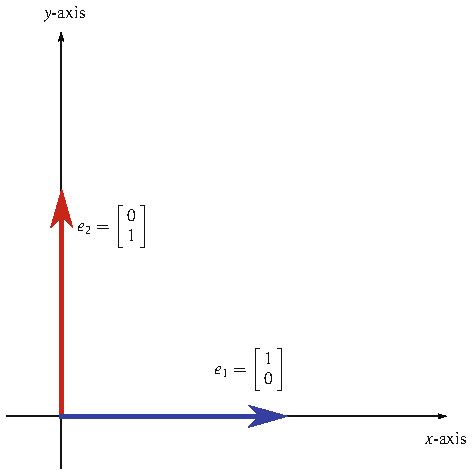
\includegraphics[width=0.561\linewidth]{images/vector/fig-1-1.pdf}
  \caption{笛卡尔平面 $\mathbb{R}^2$，其中显示了向量 $e_1$ 与 $e_2$.}
  \label{fig:1-1}
\end{figure}

\begin{question}\label{q:1-1}
考虑 $\mathbb{R}^2$，其中
\[
u=\begin{bmatrix}u_1\\u_2\end{bmatrix},\quad
v=\begin{bmatrix}v_1\\v_2\end{bmatrix},\quad
w=\begin{bmatrix}w_1\\w_2\end{bmatrix},
\]
且 $c,d\in\mathbb{R}$. 证明 $\mathbb{R}^2$ 的元素满足上述八条公理.
\end{question}

如果你学过线性代数课程，你可能记得向量空间 $V$ 的基是 $V$ 中元素的一个子集 $\beta=\{v_1,\ldots,v_n\}$，它既线性无关又张成向量空间 $V$. 线性无关意味着：如果对某些标量 $a_1,a_2,\ldots,a_n$ 有
\[
a_1v_1+a_2v_2+\cdots+a_nv_n=0,
\]
则必然 $a_1=a_2=\cdots=a_n=0$. 张成意味着：对任意 $v\in V$，都能找到标量 $a_1,a_2,\ldots,a_n$ 使得
\[
v=a_1v_1+a_2v_2+\cdots+a_nv_n.
\]
这不是一门线性代数课程，我们这里的主要目的只是提醒你线性代数中的一些事实，并让你对这些概念有更好的直觉感受，因此不再深入.

欧几里得向量空间 $\mathbb{R}^2$ 是你非常熟悉的空间，它通常被画成如图 \ref{fig:1-1} 那样的笛卡尔平面. 图中显示了两个欧几里得单位向量
\[
e_1=\binom{1}{0},\qquad e_2=\binom{0}{1}.
\]
$\mathbb{R}^2$ 中一个典型向量形如 $\begin{bmatrix}x\\y\end{bmatrix}$，其中 $x,y\in\mathbb{R}$. 容易看出 $e_1$ 与 $e_2$ 线性无关. 假设存在 $a_1$ 与 $a_2$ 使得
\[
a_1\begin{bmatrix}1\\0\end{bmatrix}+a_2\begin{bmatrix}0\\1\end{bmatrix}=\begin{bmatrix}0\\0\end{bmatrix}.
\]
这只能发生在 $a_1=0$ 且 $a_2=0$ 时，这正是为了得出 $e_1$ 与 $e_2$ 线性无关所需证明的. 要看出 $e_1$ 与 $e_2$ 张成 $\mathbb{R}^2$，我们必须证明：对 $\mathbb{R}^2$ 中任意向量 $\begin{bmatrix}x\\y\end{bmatrix}$，都能找到 $a_1$ 与 $a_2$ 使得
\[
\begin{bmatrix}x\\y\end{bmatrix}=a_1\begin{bmatrix}1\\0\end{bmatrix}+a_2\begin{bmatrix}0\\1\end{bmatrix}.
\]
但这显然可以通过令 $a_1=x$、$a_2=y$ 实现. 因此 $e_1$ 与 $e_2$ 张成 $\mathbb{R}^2$，它们被称为标准基向量，有时也称为欧几里得基向量. 显然标准基向量使用起来很方便. 当然，欧几里得单位向量集 $\{e_1,e_2\}$ 并不是 $\mathbb{R}^2$ 唯一可能的基.

\begin{question}\label{q:1-2}
证明向量集
\[
\left\{\begin{bmatrix}2\\0\end{bmatrix},\begin{bmatrix}1\\1\end{bmatrix}\right\}
\]
也是 $\mathbb{R}^2$ 的一组基. 再找出 $\mathbb{R}^2$ 的另一组基.
\end{question}

\begin{question}\label{q:1-3}
现在考虑向量空间 $\mathbb{R}^3$. 这个向量空间通常画成如图 \ref{fig:1-2} 那样. 考虑三个向量
\[
e_1=\begin{bmatrix}1\\0\\0\end{bmatrix},\qquad e_2=\begin{bmatrix}0\\1\\0\end{bmatrix},\qquad e_3=\begin{bmatrix}0\\0\\1\end{bmatrix}.
\]
\begin{enumerate}
  \item[(a)] $\mathbb{R}^3$ 中一个典型向量长什么样？
  \item[(b)] 证明 $e_1,e_2,e_3$ 线性无关.
  \item[(c)] 证明 $e_1,e_2,e_3$ 张成 $\mathbb{R}^3$.
\end{enumerate}
\end{question}

\begin{figure}[htbp]
  \centering
  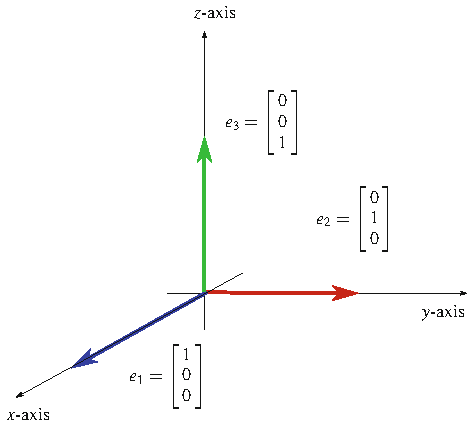
\includegraphics[width=0.562\linewidth]{images/vector/fig-1-2.pdf}
  \caption{笛卡尔空间 $\mathbb{R}^3$，其中显示了向量 $e_1,e_2,e_3$.}
  \label{fig:1-2}
\end{figure}

向量空间 $\mathbb{R}^n$ 是 $n$ 元数组
\[
\begin{bmatrix}x_1\\x_2\\\vdots\\x_n\end{bmatrix}.
\]
对它进行实际的想象是不可能的，但我们通常求助于使用与 $\mathbb{R}^3$ 的图画基本相同的 $\mathbb{R}^n$ 的``漫画式''图画. 欧几里得单位向量
\[
e_1=\begin{bmatrix}1\\0\\\vdots\\0\end{bmatrix},\quad
e_2=\begin{bmatrix}0\\1\\\vdots\\0\end{bmatrix},\quad
e_3=\begin{bmatrix}0\\0\\\vdots\\0\end{bmatrix},\quad\cdots,\quad
e_n=\begin{bmatrix}0\\0\\\vdots\\1\end{bmatrix}
\]
构成向量空间 $\mathbb{R}^n$ 的一组基，称为标准基.

本书中我们将反复做的一件事，就是帮助你建立良好而恰当的图画、漫画和心智图像，以帮助你获得对微分形式及其应用的深入而直观的理解. 有时我们会尝试绘制无法在二维或三维中精确描绘的对象. 在依据这些漫画进行思考时你必须始终小心，其中实际上丢失了大量信息. 然而，我们相信拥有适当的近似图画将大大有助于你理解当前的情形. 最后，我们强调，我们始终把向量空间的元素视为列向量，而从不视为行向量. 其原因到后面就会清楚.

现在我们来考虑向量空间之间的一类特定的变换，称为线性变换，有时也称为线性映射或线性算子. 设 $T$ 是 $\mathbb{R}^n$ 与 $\mathbb{R}^m$ 之间的映射，即 $T:\mathbb{R}^n\to\mathbb{R}^m$. 若 $T$ 具有以下两条性质，则称 $T$ 为线性变换：
\begin{enumerate}
  \item $T(v+w)=T(v)+T(w)$
  \item $T(c\cdot v)=c\cdot T(v)$
\end{enumerate}
其中 $v,w\in\mathbb{R}^n$，$c\in\mathbb{R}$.

第一条性质 $T(v+w)=T(v)+T(w)$ 意味着：对定义域向量空间中两个向量的和施行变换，与先分别对这两个向量施行变换、再在陪域向量空间中对结果求和，得到相同的结果. 第二条性质 $T(c\cdot v)=c\cdot T(v)$ 意味着：对向量的标量倍施行变换，与先对向量施行变换、再将结果乘以标量，得到相同的结果. 若 $T$ 是从 $\mathbb{R}^n$ 到 $\mathbb{R}$ 的线性变换，则它常被简称为线性函数或线性泛函.

我们先考察几个具体的例子. 考虑映射 $T:\mathbb{R}^2\to\mathbb{R}^3$，其定义为
\[
T\binom{x}{y}=\begin{bmatrix}x-y\\x+y\\2x\end{bmatrix}.
\]
首先考虑这个映射对 $\mathbb{R}^2$ 中某个具体元素的作用，
\[
T\binom{4}{10}=\begin{bmatrix}-6\\14\\8\end{bmatrix}.
\]
于是映射 $T$ 把向量 $\binom{4}{10}\in\mathbb{R}^2$ 送到向量 $\begin{bmatrix}-6\\14\\8\end{bmatrix}\in\mathbb{R}^3$. 我们现在的目标是判断映射 $T$ 是否确实是线性变换. 为此我们需要证明两条性质都成立. 从性质一开始，是否有
\[
T\left(\binom{a_1}{a_2}+\binom{b_1}{b_2}\right)=T\binom{a_1}{a_2}+T\binom{b_1}{b_2}?
\]
我们先求出左边的表达式，
\[
T\left(\binom{a_1}{a_2}+\binom{b_1}{b_2}\right)
=T\binom{a_1+b_1}{a_2+b_2}
=\begin{bmatrix}a_1+b_1-a_2-b_2\\a_1+b_1+a_2+b_2\\2a_1+2b_1\end{bmatrix}.
\]
再求出右边的表达式
\[
T\binom{a_1}{a_2}+T\binom{b_1}{b_2}
=\begin{bmatrix}a_1-a_2\\a_1+a_2\\2a_1\end{bmatrix}+\begin{bmatrix}b_1-b_2\\b_1+b_2\\2b_1\end{bmatrix}
=\begin{bmatrix}a_1+b_1-a_2-b_2\\a_1+b_1+a_2+b_2\\2a_1+2b_1\end{bmatrix}.
\]
比较这两个表达式，我们看到性质一确实成立. 接着看性质二，是否有
\[
T\left(c\cdot\binom{a_1}{a_2}\right)=c\cdot T\binom{a_1}{a_2}?
\]
求出左边的表达式，我们有
\[
T\left(c\cdot\binom{a_1}{a_2}\right)
=T\binom{ca_1}{ca_2}
=\begin{bmatrix}ca_1-ca_2\\ca_1+ca_2\\2ca_2\end{bmatrix}.
\]
再求出右边的表达式
\[
c\cdot T\binom{a_1}{a_2}
=c\cdot\begin{bmatrix}a_1-a_2\\a_1+a_2\\2a_2\end{bmatrix}
=\begin{bmatrix}ca_1-ca_2\\ca_1+ca_2\\2ca_2\end{bmatrix}.
\]
比较这两个表达式，我们看到性质二成立. 因此，由于性质一与性质二都成立，映射 $T$ 确实是一个线性变换.

\begin{question}\label{q:1-4}
考虑由
\[
T\binom{x}{y}=\binom{x+y}{y+5}
\]
定义的 $T:\mathbb{R}^2\to\mathbb{R}^2$. $T$ 是线性变换吗？
\end{question}

判断映射 $T:\mathbb{R}^n\to\mathbb{R}$ 是否为线性泛函同样直接. 考虑映射
\[
T\binom{x}{y}=2x+y.
\]
要判断 $T$ 是否为线性泛函，我们同样必须证明性质一与性质二成立. 由于
\[
T\left(\binom{a_1}{a_2}+\binom{b_1}{b_2}\right)=2a_1+2b_1+a_2+b_2
\]
且
\[
T\binom{a_1}{a_2}+T\binom{b_1}{b_2}=2a_1+2b_1+a_2+b_2,
\]
故第一条性质成立. 又由于
\[
T\left(c\cdot\binom{a_1}{a_2}\right)=2ca_1+ca_2
\]
且
\[
c\cdot T\binom{a_1}{a_2}=2ca_1+ca_2,
\]
故第二条性质成立，于是 $T$ 是一个线性泛函.

\begin{question}\label{q:1-5}
考虑下面定义的 $T:\mathbb{R}^2\to\mathbb{R}$. 它们是线性泛函吗？
\begin{enumerate}
  \item[(a)] $T\binom{x}{y}=x^2+y$
  \item[(b)] $T\binom{x}{y}=xy$
  \item[(c)] $T\binom{x}{y}=2x+3y+7$
\end{enumerate}
\end{question}

在把注意力转向线性变换与矩阵之间的关系之前，我们非常简要地回顾一下矩阵与矩阵乘法. 简单地说，矩阵就是一个矩形数表，一般写在方括号内. 例如，
\[
\begin{bmatrix}7&4&-3\\2&-9&5\end{bmatrix},\qquad
\begin{bmatrix}2&-6\\9&4\\11&1\\6&8\end{bmatrix},\qquad
\begin{bmatrix}2&-4&6&7\\-1&8&0&10\\5&2&-3&7\\-2&-4&1&3\end{bmatrix}
\]
都是矩阵的例子. 矩阵的大小用行数和列数表示，通常写作（行数）$\times$（列数）. 例如，上述矩阵的大小分别是 $2\times3$、$4\times2$ 和 $4\times4$. 矩阵中的数有时称为矩阵元素，用带两个下标的变量表示，第一个下标是行号，第二个下标是列号. 这里用一个 $3\times3$ 矩阵展示带下标变量的写法，
\[
\begin{bmatrix}a_{11}&a_{12}&a_{13}\\a_{21}&a_{22}&a_{23}\\a_{31}&a_{32}&a_{33}\end{bmatrix}.
\]
重要的是要记住，行下标在前，列下标在后.

如果你以前从未见过矩阵乘法，它可能看起来有些复杂. 首先，第一个矩阵的列数必须等于第二个矩阵的行数. 其次，乘积矩阵中第 $ij$ 个元素由第一个矩阵的第 $i$ 行与第二个矩阵的第 $j$ 列相乘得到. 在给出一般公式之前，我们先用一个例子说明，
\[
\begin{bmatrix}1&2\\3&4\end{bmatrix}\begin{bmatrix}5&6\\7&8\end{bmatrix}.
\]
乘积矩阵的 $a_{11}$ 项由红色行与蓝色列相乘得到，即
\[
a_{11}=1\cdot5+2\cdot7=19.
\]
类似地，
\begin{align*}
\begin{bmatrix}1&2\\3&4\end{bmatrix}\begin{bmatrix}5&6\\7&8\end{bmatrix}
\Rightarrow a_{12}=1\cdot6+2\cdot8=22, \\
\begin{bmatrix}1&2\\3&4\end{bmatrix}\begin{bmatrix}5&6\\7&8\end{bmatrix}
\Rightarrow a_{21}=3\cdot5+4\cdot7=43, \\
\begin{bmatrix}1&2\\3&4\end{bmatrix}\begin{bmatrix}5&6\\7&8\end{bmatrix}
\Rightarrow a_{22}=3\cdot6+4\cdot8=50.
\end{align*}
把所有这些放在一起，我们得到
\[
\begin{bmatrix}1&2\\3&4\end{bmatrix}\begin{bmatrix}5&6\\7&8\end{bmatrix}
=\begin{bmatrix}19&22\\43&50\end{bmatrix}.
\]

现在我们给出矩阵乘法的一般公式. 若 $A$ 是 $n\times m$ 矩阵，$B$ 是 $m\times p$ 矩阵，
\[
\begin{bmatrix}
a_{11}&a_{12}&\cdots&a_{1m}\\
a_{21}&a_{22}&\cdots&a_{2m}\\
\vdots&\vdots&\ddots&\vdots\\
a_{n1}&a_{n2}&\cdots&a_{nm}
\end{bmatrix}
\begin{bmatrix}
b_{11}&b_{12}&\cdots&b_{1p}\\
b_{21}&b_{22}&\cdots&b_{2p}\\
\vdots&\vdots&\ddots&\vdots\\
b_{m1}&b_{m2}&\cdots&b_{mp}
\end{bmatrix}
=
\begin{bmatrix}
c_{11}&c_{12}&\cdots&c_{1p}\\
c_{21}&c_{22}&\cdots&c_{2p}\\
\vdots&\vdots&\ddots&\vdots\\
c_{n1}&c_{n2}&\cdots&c_{np}
\end{bmatrix},
\]
其中
\[
c_{ij}=\sum_{k=1}^{m}a_{ik}b_{kj}.
\]
注意乘积矩阵的维数是 $n\times p$.

现在我们转向线性变换与矩阵之间的关系. 这不是一门线性代数课程，所以我们不会在向量空间或基上大做文章. 我们只使用向量空间 $\mathbb{R}^n$ 以及由欧几里得单位向量 $e_1,e_2,\ldots,e_n$ 组成的标准基. 严格地说，要把线性变换 $T:\mathbb{R}^n\to\mathbb{R}^m$ 写成矩阵，我们必须为 $\mathbb{R}^n$ 和 $\mathbb{R}^m$ 各取一个有序基；也就是说，基元素必须有一个固定的顺序. 但我们通常认为欧几里得单位向量具有直观上显而易见的顺序，$e_1$ 第一，$e_2$ 第二，$e_3$ 第三，依此类推. 在给出一般定义之前，我们先看几个例子.

考虑我们之前的例子，由
\[
T\binom{x}{y}=\begin{bmatrix}x-y\\x+y\\2x\end{bmatrix}
\]
定义的 $T:\mathbb{R}^2\to\mathbb{R}^3$. 利用线性变换的性质以及矩阵乘法的知识，我们有以下过程
\begin{align*}
T\binom{x}{y}
&=T\left(\binom{x}{0}+\binom{0}{y}\right)\\
&=T\left(x\binom{1}{0}+y\binom{0}{1}\right)\\
&=T\left(x\binom{1}{0}\right)+T\left(y\binom{0}{1}\right) &&\text{性质一}\\
&=xT\binom{1}{0}+yT\binom{0}{1} &&\text{性质二}\\
&=x\begin{bmatrix}1\\1\\2\end{bmatrix}+y\begin{bmatrix}-1\\1\\0\end{bmatrix}\\
&=\begin{bmatrix}1&-1\\1&1\\2&0\end{bmatrix}\binom{x}{y} &&\text{矩阵乘法的定义}
\end{align*}
通过比较左右两端，我们可以看出可以把线性变换 $T$ 写成一个矩阵，即
\[
T\equiv\begin{bmatrix}1&-1\\1&1\\2&0\end{bmatrix}.
\]

这个计算对你来说可能显而易见，你也许会奇怪我们为什么要经历这些步骤. 主要原因是说明答案如何依赖于 $T$ 在 $\mathbb{R}^2$ 的基向量上的作用. 让我们更详细地考虑这一点. 首先让 $T$ 作用在 $\mathbb{R}^2$ 的第一个基向量上，得到
\[
T\binom{1}{0}=\begin{bmatrix}1\\1\\2\end{bmatrix}=1\begin{bmatrix}1\\0\\0\end{bmatrix}+1\begin{bmatrix}0\\1\\0\end{bmatrix}+2\begin{bmatrix}0\\0\\1\end{bmatrix}.
\]
注意 $\mathbb{R}^3$ 的基向量的系数正是 $T$ 的矩阵表示的第一列的各个元素. 类似地，让 $T$ 作用在 $\mathbb{R}^2$ 的第二个基向量上，得到
\[
T\binom{0}{1}=\begin{bmatrix}-1\\1\\0\end{bmatrix}=-1\begin{bmatrix}1\\0\\0\end{bmatrix}+1\begin{bmatrix}0\\1\\0\end{bmatrix}+0\begin{bmatrix}0\\0\\1\end{bmatrix}.
\]
这里 $\mathbb{R}^3$ 的基向量的系数正是 $T$ 的矩阵表示的第二列的各个元素.

现在给出线性变换的矩阵表示的形式定义. 设 $T:\mathbb{R}^n\to\mathbb{R}^m$. 令 $e_1,e_2,\ldots,e_n$ 为 $\mathbb{R}^n$ 的标准基，令 $\tilde{e}_1,\tilde{e}_2,\ldots,\tilde{e}_m$ 为 $\mathbb{R}^m$ 的标准基. 则对 $1\leq j\leq n$，存在唯一的数 $a_{ij}$ 使得
\[
T(e_j)=\sum_{i=1}^{m}a_{ij}\tilde{e}_i.
\]
于是 $T$ 的矩阵表示就是元素为 $a_{ij}$ 的 $m\times n$ 矩阵.

\begin{question}\label{q:1-6}
求线性变换
\[
T\binom{x}{y}=\begin{bmatrix}2x+3y\\0\\2x-5y\end{bmatrix}
\]
的矩阵表示.
\end{question}

现在我们转向线性泛函，它是陪域为 $\mathbb{R}$ 的线性变换这一特例. 考虑之前的线性泛函 $T\binom{x}{y}=2x+y$. 我们求这个线性泛函的矩阵表示，
\[
T\binom{x}{y}=2x+y=[2,1]\binom{x}{y}.
\]
可以看出线性泛函的矩阵表示是 $1\times n$ 矩阵，也就是行向量. 这是重要的一点：线性泛函用行向量表示. 当我们写 $1\times n$ 矩阵（即行向量）时，通常在元素之间加逗号，只是为了使一切清楚.

本节最后一个主要主题是对偶空间的定义. 假设给定一个向量空间 $V$. 在本书中我们考虑的向量空间只有对某个整数 $n$ 的 $\mathbb{R}^n$. $V$ 上所有线性泛函的集合称为 $V$ 的对偶空间，记为 $V^*$.

事实上，$V$ 的对偶空间 $V^*$ 本身也是一个向量空间. 为证明这一点，我们先说明线性泛函的加法意味着什么. 我们可以把两个线性泛函 $S:V\to\mathbb{R}$ 与 $T:V\to\mathbb{R}$ 相加，得到一个新的线性泛函 $S+T:V\to\mathbb{R}$，泛函 $S+T$ 的取值正如你所预期的那样，$(S+T)(v)=S(v)+T(v)$，其中 $v\in V$. 为了证明向量空间 $V$ 的对偶空间 $V^*$（即 $V$ 上线性泛函的集合）本身是一个向量空间，我们必须证明八条向量空间公理都得到满足.

考虑我们写为 $v+w=w+v$ 的第一条公理，其中 $v,w$ 是向量空间的元素. 但现在我们面对的是 $V^*$，其元素为 $S$ 与 $T$. 我们要证明 $S+T=T+S$. 该怎么做呢？我们必须利用线性泛函加法的定义. 对任意元素 $v\in V$，有 $(S+T)(v)=S(v)+T(v)$. 现在回想 $S(v)$ 与 $T(v)$ 都只是实数，而实数加法是交换的，因此 $S(v)+T(v)=T(v)+S(v)$. 最后，利用线性泛函的加法，有 $T(v)+S(v)=(T+S)(v)$. 把这一切放在一起，我们得到 $(S+T)(v)=(T+S)(v)$. 由于这对任意 $v\in V$ 都成立，我们可以写 $S+T=T+S$，从而证明第一条公理得到满足.

\begin{question}\label{q:1-7}
设 $R,S,T:\mathbb{R}^n\to\mathbb{R}$ 是 $V$ 上的线性泛函，即 $R,S,T\in V^*$，且 $c,d$ 是实数. 通过证明其余七条向量空间公理也得到满足，证明 $V^*$ 是一个向量空间.
\end{question}

我们继续考虑具体的向量空间 $\mathbb{R}^2$. 任意元素 $\binom{x}{y}\in\mathbb{R}^2$ 都可以写成
\[
\binom{x}{y}=x\binom{1}{0}+y\binom{0}{1}.
\]
设 $T\in(\mathbb{R}^2)^*$，则
\begin{align*}
T\binom{x}{y}
&=T\left(x\binom{1}{0}+y\binom{0}{1}\right)\\
&=T\left(x\binom{1}{0}\right)+T\left(y\binom{0}{1}\right)\\
&=xT\binom{1}{0}+yT\binom{0}{1}\\
&=xc_1+yc_2
\end{align*}
其中 $c_1=T\binom{1}{0}$、$c_2=T\binom{0}{1}$ 是某些实数. 所以线性泛函 $T\in(\mathbb{R}^2)^*$ 对任意向量 $\binom{x}{y}\in\mathbb{R}^2$ 的作用完全由它在基向量 $\binom{1}{0}$ 与 $\binom{0}{1}$ 上的作用决定. 我们定义两个线性泛函 $T_1$ 与 $T_2$，使它们在这些基向量上的作用如下：
\[
T_1\binom{1}{0}=1,\qquad T_1\binom{0}{1}=0
\]
以及
\[
T_2\binom{1}{0}=0,\qquad T_2\binom{0}{1}=1.
\]

\begin{question}\label{q:1-8}
设 $T_1$ 与 $T_2$ 是上面定义的 $\mathbb{R}^2$ 上的线性泛函.
\begin{enumerate}
  \item[(a)] 证明 $T_1\binom{x}{y}=x$，$T_2\binom{x}{y}=y$.
  \item[(b)] 是否可能把上面的线性泛函 $T$ 写成 $T_1$ 与 $T_2$ 的线性组合？
  \item[(c)] 证明 $\{T_1,T_2\}$ 是 $(\mathbb{R}^2)^*$（即 $\mathbb{R}^2$ 上线性泛函的集合）的一组基.
\end{enumerate}
\end{question}

既然对偶空间是向量空间，那么对偶空间当然有基. 使用欧几里得单位向量的标准记号，
\[
e_1=\binom{1}{0},\qquad e_2=\binom{0}{1},
\]
我们可以写 $T_1(e_1)=1$、$T_2(e_1)=0$、$T_1(e_2)=0$、$T_2(e_2)=1$. 用稍许不同的记号，我们可以把它概括为 $T_i(e_j)=\delta_{ij}$，$i,j=1,2$，其中 $\delta_{ij}$ 称为 \newterm{kronecker-delta}{克罗内克 $\delta$ 函数}{Kronecker delta function}，其定义为
\[
\delta_{ij}=\begin{cases}1&i=j\\0&i\neq j.\end{cases}
\]
由于 $T_i(e_j)=\delta_{ij}$，我们称 $T_1$ 与向量 $e_1$ 对偶，称 $T_2$ 与向量 $e_2$ 对偶，并称 $\{T_1,T_2\}$ 为 $\{e_1,e_2\}$ 的对偶基.

现在引入一点记号，我们常常把 $T_1$ 写成 $e^1$，把 $T_2$ 写成 $e^2$. 注意这里用的是上标而不是下标. 于是我们有 $\{e_1,e_2\}$ 是 $\mathbb{R}^2$ 的标准基，而 $\{e^1,e^2\}$ 是它的对偶基，是对偶空间 $(\mathbb{R}^2)^*$ 的一组基. 我们还常常写 $e^i(e_j)=\delta_j^i$，这与上面定义的克罗内克 $\delta$ 函数完全相同，只是其中一个下标写成上标，以与基元素和对偶基元素上的上下标写法相匹配.

另外，注意 $e^i(e_j)$ 本质上就是函数记号，线性泛函 $e^i$ 以向量 $e_j$ 作为其自变量. 有时这也写作 $\langle e^i,e_j\rangle$.

还回想起我们前面说过，像 $\mathbb{R}^2$ 这样的向量空间的元素总是写成列向量，而微积分课程中通常不采用这一约定，那里的向量常常为了方便写成行向量. 我们在此坚持这一约定的原因是，像 $(\mathbb{R}^2)^*$ 这样的对偶空间的元素总是写成行向量. 由于 $e^1=1\cdot e^1+0\cdot e^2$，我们写 $e^1=[1,0]$. 类似地，由于 $e^2=0\cdot e^1+1\cdot e^2$，我们有 $e^2=[0,1]$. 这使我们能够使用矩阵乘法：
\begin{align*}
e^1(e_1)&=\langle e^1,e_1\rangle=[1,0]\binom{1}{0}=1\\
e^1(e_2)&=\langle e^1,e_2\rangle=[1,0]\binom{0}{1}=0\\
e^2(e_1)&=\langle e^2,e_1\rangle=[0,1]\binom{1}{0}=0\\
e^2(e_2)&=\langle e^2,e_2\rangle=[0,1]\binom{0}{1}=1
\end{align*}
注意这与我们使用克罗内克 $\delta$ 记号得到的结果一致. 正如 $\mathbb{R}^2$ 中任意元素 $v$ 可以写成 $e_1$ 与 $e_2$ 的线性组合并写成列向量，
\[
v=xe_1+ye_2=\binom{x}{y},
\]
$(\mathbb{R}^2)^*$ 中任意元素 $\alpha$ 也可以写成 $e^1$ 与 $e^2$ 的线性组合并写成行向量
\[
\alpha=ae^1+be^2=[a,b].
\]
于是我们可以用矩阵乘法求出
\[
\alpha(v)=\langle\alpha,v\rangle=[a,b]\binom{x}{y}=ax+by.
\]

所有这些当然可以推广到任意向量空间 $V$，而且你会经常（虽然不是总是）看到 $V$ 的基元素用下标书写，$V^*$ 的基元素用上标书写. 例如，若 $\{v_1,v_2,\ldots,v_n\}$ 是某个向量空间 $V$ 的基，则我们把它在 $V^*$ 中的对偶基写为 $\{v^1,v^2,\ldots,v^n\}$. 于是任意 $v\in V$ 都可以写成 $\{v_1,v_2,\ldots,v_n\}$ 的线性组合，从而写成列向量；任意 $\alpha\in V^*$ 都可以写成 $\{v^1,v^2,\ldots,v^n\}$ 的线性组合，从而写成行向量. 这使得 $\alpha(v)$ 可以通过矩阵乘法计算，即行向量乘以列向量. 这也解释了为什么我们总是把向量空间的元素写成列向量：因为对偶空间的元素写成行向量，而始终区分向量空间元素与对偶空间元素非常重要. 在向量微积分课程中不引入对偶空间，因此为了方便，向量有时写成行向量. 我们在本书中绝不这样做.

\begin{question}\label{q:1-9}
考虑带标准欧几里得基
\[
e_1=\begin{bmatrix}1\\0\\0\end{bmatrix},\qquad e_2=\begin{bmatrix}0\\1\\0\end{bmatrix},\qquad e_3=\begin{bmatrix}0\\0\\1\end{bmatrix}
\]
的向量空间 $\mathbb{R}^3$. 令
\[
v=\begin{bmatrix}x\\y\\z\end{bmatrix}=xe_1+ye_2+ze_3\in\mathbb{R}^3.
\]
设 $(\mathbb{R}^3)^*$ 为 $\mathbb{R}^3$ 的对偶空间，其对偶基为
\[
e^1=[1,0,0],\qquad e^2=[0,1,0],\qquad e^3=[0,0,1].
\]
现在考虑线性泛函
\[
f\begin{pmatrix}\begin{bmatrix}x\\y\\z\end{bmatrix}\end{pmatrix}=3x+2y-6z.
\]
\begin{enumerate}
  \item[(a)] 验证 $f$ 确实是一个线性泛函.
  \item[(b)] 令 $v=\begin{bmatrix}-3\\4\\7\end{bmatrix}$. 求 $f(v)$.
  \item[(c)] 对 $i=1,2,3$ 求 $f(e_i)$.
  \item[(d)] 把 $f$ 写成 $e^1,e^2,e^3$ 的线性组合.
  \item[(e)] 把 $f\in(\mathbb{R}^3)^*$ 写成行向量.
  \item[(f)] 用矩阵乘法写出 $f(v)$.（即行向量 $f$ 乘以列向量 $v$.）
\end{enumerate}
\end{question}

\begin{question}\label{q:1-10}
考虑带标准欧几里得基 $e_1,e_2,e_3,e_4$ 的向量空间 $\mathbb{R}^4$，以及带标准对偶基 $e^1,e^2,e^3,e^4$ 的对偶空间 $(\mathbb{R}^4)^*$. 令
\[
v=\begin{bmatrix}x_1\\x_2\\x_3\\x_4\end{bmatrix}\in\mathbb{R}^4,
\]
并定义线性泛函 $f$ 为 $f(v)=5x_1-2x_2+7x_3-6x_4$.
\begin{enumerate}
  \item[(a)] 验证 $f\in(\mathbb{R}^4)^*$.（即 $f$ 是一个线性泛函.）
  \item[(b)] 对 $i=1,2,3,4$ 求 $f(e_i)$，并据此把 $f$ 写成行向量.
  \item[(c)] 用表示 $f$ 的行向量求
  \[
  f\begin{pmatrix}\begin{bmatrix}-7\\3\\2\\-1\end{bmatrix}\end{pmatrix}
  \qquad\text{与}\qquad
  f\begin{pmatrix}\begin{bmatrix}1/2\\-4\\-2/3\\5\end{bmatrix}\end{pmatrix}.
  \]
\end{enumerate}
\end{question}

让我们更仔细地看看对偶基元素. 以 $(\mathbb{R}^4)^*$ 为例，我们考虑对偶基元素 $e^1,e^2,e^3,e^4$. 考虑 $\mathbb{R}^4$ 中的如下向量，
\[
v=\begin{bmatrix}2\\-5\\7\\-9\end{bmatrix}.
\]
让我们看看对偶基元素如何作用于 $v$. 我们有
\[
e^1(v)=[1,0,0,0]\begin{bmatrix}2\\-5\\7\\-9\end{bmatrix}=2.
\]
类似地，有 $e^2(v)=-5$、$e^3(v)=7$、$e^4(v)=-9$. 可以看出，本质上对偶基元素``挑出''相应的向量坐标：$e^1$ 挑出第一个坐标，$e^2$ 挑出第二个坐标，$e^3$ 挑出第三个坐标，$e^4$ 挑出第四个坐标.

现在我们将探讨常被用来描绘线性泛函的漫画之一. 我们有意使用``漫画''这个词. 我们所建立的是一些不完美的心智图像，以便尝试想象正在发生的事情. 重要的是要记住这些图像并不精确，然而它们使我们能够发展对数学概念的直觉. 根据我们的经验，我们将在这里开始建立的这种漫画表示在物理学中最常见. 我们用 $\mathbb{R}^2$ 和 $(\mathbb{R}^2)^*$ 作为示例空间开始.

令
\[
e_1=\binom{1}{0},\qquad e_2=\binom{0}{1}
\]
为向量空间 $\mathbb{R}^2$ 的一组基. 这组基诱导出 $(\mathbb{R}^2)^*$ 的对偶基 $e^1=[1,0]$ 与 $e^2=[0,1]$. 考虑 $\mathbb{R}^2$ 中的如下向量：
\[
\binom{1}{3},\ \binom{1}{2},\ \binom{1}{1},\ \binom{1}{0},\ \binom{1}{-1},\ \binom{1}{-2},\ \binom{1}{-3}.
\]
显然 $e^1$ 作用于这些向量中的每一个都给出 $1$. 现在考虑向量：
\[
\binom{2}{3},\ \binom{2}{2},\ \binom{2}{1},\ \binom{2}{0},\ \binom{2}{-1},\ \binom{2}{-2},\ \binom{2}{-3}.
\]
我们有 $e^1$ 把所有这些向量送到 $2$. 以同样的方式，$e^1$ 把任意形如 $\binom{0}{y}$（其中 $y\in\mathbb{R}$）的向量送到 $0$. 它把任意形如 $\binom{-1}{y}$ 的向量送到 $-1$，依此类推. 如图 \ref{fig:1-3} 那样画出这些向量，可以看出：$e^1$ 送到 $1$ 的那些向量的终点位于竖直线 $x=1$ 上，$e^1$ 送到 $2$ 的那些向量的终点位于竖直线 $x=2$ 上，$e^1$ 送到 $0$ 的那些向量的终点位于竖直线 $x=0$ 上，$e^1$ 送到 $-1$ 的那些向量的终点位于竖直线 $x=-1$ 上，依此类推. 这给出了一种构造线性泛函 $e^1$ 的漫画图像的方法，即在向量空间 $\mathbb{R}^2$ 上画出整数水平集，如图 \ref{fig:1-4} 所示. 考虑图中所示的向量，
\[
A=\binom{3.5}{1.5},\qquad B=\binom{-3.5}{1.5},\qquad C=\binom{1.9}{-1},\qquad D=\binom{-1.5}{-1.5},
\]
显然 $e^1(A)=3.5$、$e^1(B)=-3.5$、$e^1(C)=1.9$、$e^1(D)=-1.5$.

\begin{figure}[htbp]
  \centering
  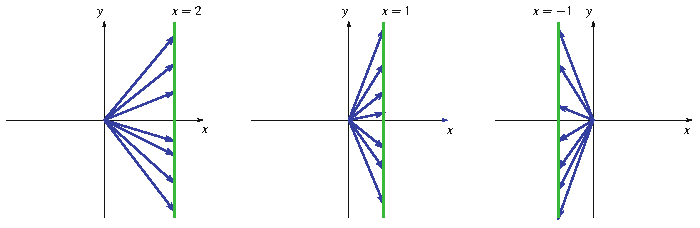
\includegraphics[width=0.960\linewidth]{images/vector/fig-1-3.pdf}
  \caption{终点的 $x$ 值分别为 $2$、$1$、$-1$ 的向量草图}
  \label{fig:1-3}
\end{figure}

\begin{figure}[htbp]
  \centering
  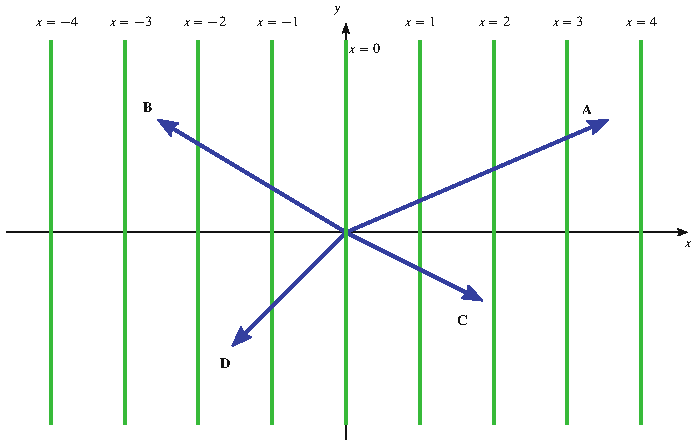
\includegraphics[width=0.915\linewidth]{images/vector/fig-1-4.pdf}
  \caption{向量空间 $\mathbb{R}^2$ 上描绘线性泛函 $e^1$ 的``水平集''，以及向量 $A,B,C,D$}
  \label{fig:1-4}
\end{figure}

使用 $e^1$ 的这幅漫画图像只能给出近似答案，但它提供了一种很好的方式来可视化和理解 $e^1$ 的作用. 有时在物理学中你会听到这样的说法：线性泛函所给出的``向量的值''，等于该向量刺穿的该线性泛函的水平集的个数. 本质上，线性泛函 $e^1$ 的这幅图像通过数向量``刺穿''或穿过的竖直水平集的个数来起作用，同时仍然记录符号. 也就是说，我们把负的水平集计为负的. 如果向量的终点落在一个水平集上，则该水平集被视为被``刺穿''，并计入总数. 例如，在图 \ref{fig:1-4} 中，向量 $A$ 刺穿 3 个水平集，向量 $C$ 刺穿 1 个水平集，而向量 $B$ 刺穿 $-3$ 个水平集，向量 $D$ 刺穿 $-1$ 个水平集. 因此，根据我们的漫画图像，有 $e^1(A)=3$、$e^1(B)=-3$、$e^1(C)=1$、$e^1(D)=-1$，这与实际值很接近. 类似的分析得到 $e^2$ 如图 \ref{fig:1-5} 所示.

\begin{question}\label{q:1-11}
考虑线性泛函 $e^2\in(\mathbb{R}^2)^*$.
\begin{enumerate}
  \item[(a)] 给出 $e^2$ 送到 $1$、$2$、$0$、$-1$ 的五个向量.
  \item[(b)] 画出这些向量，并用它们的终点画出水平集.
\end{enumerate}
\end{question}

\begin{figure}[htbp]
  \centering
  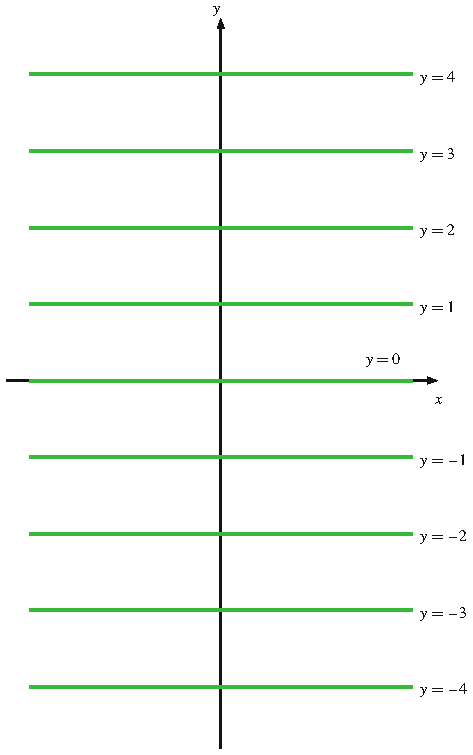
\includegraphics[width=0.561\linewidth]{images/vector/fig-1-5.pdf}
  \caption{向量空间 $\mathbb{R}^2$ 上描绘线性泛函 $e^2$ 的``水平集''}
  \label{fig:1-5}
\end{figure}

想一想 $e^1$ 与 $e^2$ 的两幅漫画. $xy$ 坐标轴代表向量空间 $\mathbb{R}^2$. 然而 $e^1$ 与 $e^2$ 实际上位于对偶空间 $(\mathbb{R}^2)^*$ 中. 在某种意义上我们做的事情很奇怪，我们试图在 $\mathbb{R}^2$ 中画出 $e^1$ 与 $e^2$ 的图像，而它们是 $(\mathbb{R}^2)^*$ 的元素. 考虑我们在 $\mathbb{R}^2$ 中画的 $e^1$ 的图与图 \ref{fig:1-6} 中我们在 $(\mathbb{R}^2)^*$ 中画的 $e^1$ 的图有多么不同. 类似地，我们在 \ref{fig:1-7} 中画出 $e^2$ 在 $\mathbb{R}^2$ 中的图与 $e^2$ 在 $(\mathbb{R}^2)^*$ 中的图.

\begin{figure}[htbp]
  \centering
  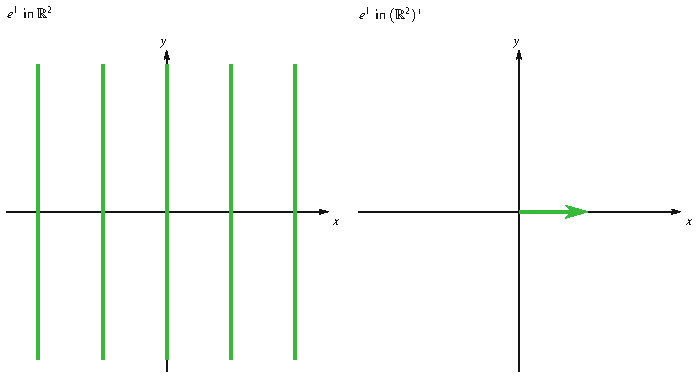
\includegraphics[width=0.929\linewidth]{images/vector/fig-1-6.pdf}
  \caption{描绘线性泛函 $e^1$ 的水平集：画在向量空间 $\mathbb{R}^2$ 上（左），以及把线性泛函 $e^1$ 画成向量空间 $(\mathbb{R}^2)^*$ 中的向量（右）}
  \label{fig:1-6}
\end{figure}

\begin{figure}[htbp]
  \centering
  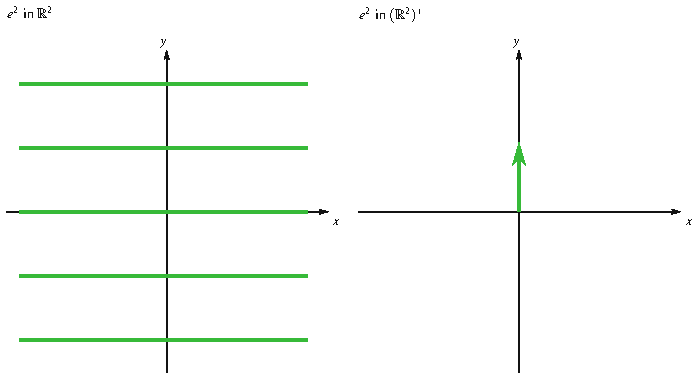
\includegraphics[width=0.929\linewidth]{images/vector/fig-1-7.pdf}
  \caption{描绘线性泛函 $e^2$ 的水平集：画在向量空间 $\mathbb{R}^2$ 上（左），以及把线性泛函 $e^2$ 画成向量空间 $(\mathbb{R}^2)^*$ 中的向量（右）}
  \label{fig:1-7}
\end{figure}

现在我们来看一个稍复杂的线性泛函 $f=2e^1+e^2\in(\mathbb{R}^2)^*$. 首先问自己：$f$ 把哪些向量 $v$ 送到 $1$？即求满足 $f(v)=1$ 的 $v$：
\begin{align*}
1=f\binom{x}{y}=2e^1\binom{x}{y}+e^2\binom{x}{y}=2x+y \\
\Rightarrow\quad 2x+y=1\quad\Rightarrow\quad y=-2x+1.
\end{align*}
换句话说，$\Rightarrow f\binom{x}{-2x+1}=1$，其中 $x$ 是任意实数. 我们还发现，线性泛函 $f$ 送到 $1$ 的那些向量 $v$ 的终点确定直线 $y=-2x+1$. 因此我们的 $1$ 的水平集由方程 $y=-2x+1$ 给出.

\begin{question}\label{q:1-12}
求 $f$ 送到 $2$、$3$、$0$、$-1$、$-2$ 的向量. 用这些向量确定这些值对应的水平集.
\end{question}

把我们在问题中找到的 $f$ 的水平集画出来，就得到 $f$ 在 $\mathbb{R}^2$ 上的图像，如图 \ref{fig:1-8} 所示. 考虑图中所示的两个向量，
\[
A=\binom{1/2}{1},\qquad B=\binom{1}{-3}.
\]

\begin{figure}[htbp]
  \centering
  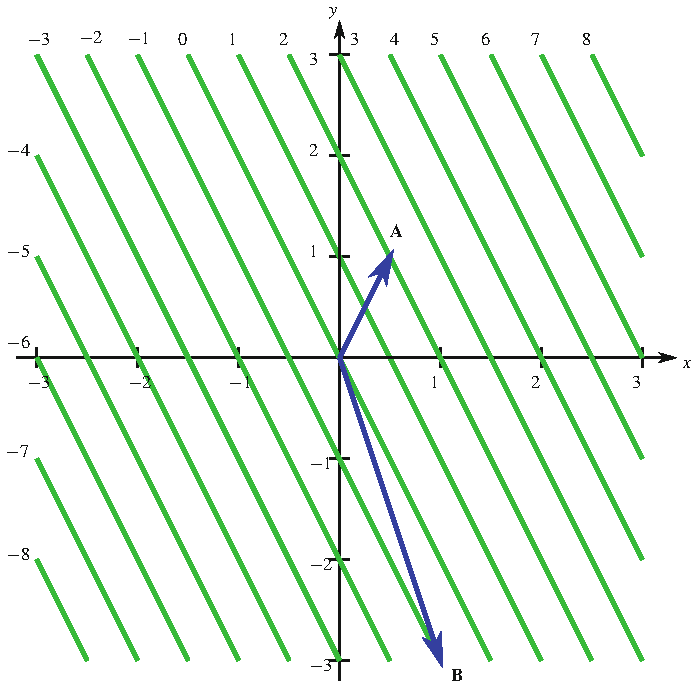
\includegraphics[width=0.826\linewidth]{images/vector/fig-1-8.pdf}
  \caption{向量空间 $\mathbb{R}^2$ 上描绘线性泛函 $f=2e^1+e^2$ 的水平集，以及向量 $A$ 与 $B$}
  \label{fig:1-8}
\end{figure}

显然 $A$ 刺穿两个水平集，因此根据我们的图像 $f(A)=2$；而 $B$ 刺穿 $-1$ 个水平集，因此根据我们的图像 $f(B)=-1$. 用计算来复核我们的图像，我们有
\begin{align*}
f(A)=2e^1(A)+e^2(A)=2\cdot\frac12+1=2 \\
f(B)=2e^1(B)+e^2(B)=2(1)-3=-1,
\end{align*}
这正是我们所预期的. 线性泛函的漫画图像可以很容易地推广到 $\mathbb{R}^3$. 我们这里不这样做，但我们将在后面的一章中在稍许不同的背景下考虑这种情况.

\section{体积与行列式}

矩阵的行列式具有广泛的性质和用途. 然而，对我们来说，行列式最有用的地方在于它与体积的联系：矩阵的行列式给出由矩阵各列给出的向量所张成的平行六面体的有向体积. 它与我们对体积的直观概念的唯一区别在于，这里的体积带有正号或负号. 因此，虽然我们习惯于认为体积是正的（或零），但事实上它也可以是负的. 而如果说这还不够奇怪的话，真正离奇的是，我们对体积应有行为的直觉观念恰恰迫使我们接受这个符号.

行列式有各种各样的引入方式，坦白说，其中许多方式一点也不清楚. 由于真正理解行列式与体积的关系对我们很重要，我们将实际利用对体积的直观理解以及我们期望体积具有的三条性质来推导行列式. 令人惊叹的是，体积应有行为的这三条性质唯一地确定了行列式.

那么，我们期望体积如何表现？首先，我们期望单位立方体（就这件事而言，单位 $n$ 立方体）的体积为 1. 这源于 $1^3$（或 $1^n$）等于 1 这一事实. 这实际上对我们的体积进行了归一化. 其次，我们期望退化平行六面体的体积为零. 基本上，在 $n$ 维空间中，任何 $n-1$ 维对象的 $n$ 维体积都是零. 例如，$\mathbb{R}^3$ 中的一个二维单位正方形具有零三维体积，即使在 $\mathbb{R}^2$ 中它的二维体积为 1. 第三，我们期望体积是线性的. 线性意味着几件事，其中之一是：如果固定 $n$ 维平行六面体的 $n-1$ 条边，并把剩下的一条边按某个因子缩放，那么平行六面体的体积也按该因子改变. 所以，如果我们把 3 立方体一条边的长度加倍，那么体积也将加倍. 现在，带着这些一般想法，让我们进入实际的数学.

假设我们有一个平行六面体 $P\in\mathbb{R}^n$，其边由 $v_1,v_2,\ldots,v_n\in\mathbb{R}^n$ 给出. 我们说平行六面体 $P$ 是向量 $v_1,v_2,\ldots,v_n$ 的张成，并写 $P=\mathrm{span}\{v_1,v_2,\ldots,v_n\}$. 注意这里``张成''一词的用法与上一节不同，上一节我们说向量空间的基张成该向量空间. 我们想找一个函数 $D:\mathbb{R}^{n\times n}\to\mathbb{R}$，它把 $v_1,v_2,\ldots,v_n$（或者类似地，以 $v_1,v_2,\ldots,v_n$ 为列的矩阵 $M$）送到一个实数，即 $P$ 的体积. 让记号灵活一些，我们既可以写 $D(M)$，也可以写 $D(v_1,v_2,\ldots,v_n)$. 现在，我们用数学的严谨性来表述体积的三条直观性质.

\begin{property}{1}\label{prop:1-1}
$D(I)=1$，其中 $I=[e_1,e_2,\ldots,e_n]$，即单位矩阵.
\end{property}

这说的是单位 $n$ 立方体的体积为 1. 二维和三维的例子如图 \ref{fig:1-9} 所示. 注意单位 $n$ 立方体由 $\mathrm{span}\{e_1,e_2,\ldots,e_n\}$ 给出，而单位矩阵 $I$ 由 $I=[e_1,e_2,\ldots,e_n]$ 给出. 因此我们也常常用 $I$ 来记单位 $n$ 立方体.

\begin{figure}[htbp]
  \centering
  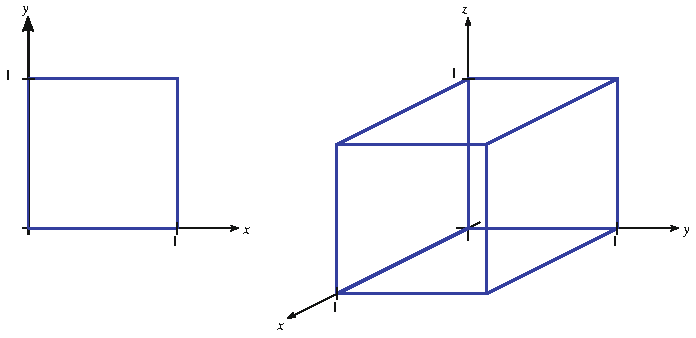
\includegraphics[width=0.856\linewidth]{images/vector/fig-1-9.pdf}
  \caption{单位正方形的二维体积（即面积）为 $1$（左），单位立方体的三维体积也为 $1$（右）}
  \label{fig:1-9}
\end{figure}

\begin{property}{2}\label{prop:1-2}
若对任意 $i\neq j$ 有 $v_i=v_j$，则 $D(v_1,v_2,\ldots,v_n)=0$.
\end{property}

这条性质说的是，如果 $n$ 平行六面体的任意两条边相同，也就是说，如果平行六面体是退化的，那么体积为零. 图 \ref{fig:1-10} 在三维空间中的二维平行六面体上展示了这一点.

\begin{figure}[htbp]
  \centering
  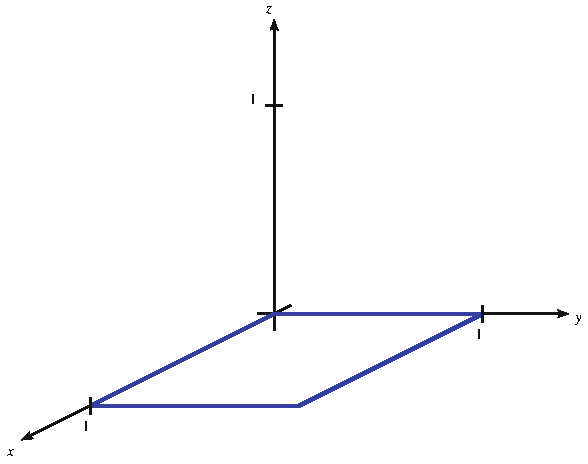
\includegraphics[width=0.721\linewidth]{images/vector/fig-1-10.pdf}
  \caption{三维空间中二维平行六面体的三维体积为零}
  \label{fig:1-10}
\end{figure}

\begin{property}{3}\label{prop:1-3}
$D$ 是线性的. 即，对任意 $j=1,\ldots,n$，
\begin{align*}
D(v_1,\ldots,v_{j-1},v+cw,v_{j+1},\ldots,v_n)
&=D(v_1,\ldots,v_{j-1},v,v_{j+1},\ldots,v_n)\\
&\quad+c\,D(v_1,\ldots,v_{j-1},w,v_{j+1},\ldots,v_n).
\end{align*}
\end{property}

实际上，这说的比``如果我们把一条边的长度按因子缩放，体积也按该因子缩放''稍多一点. 这条性质还包括剪切，但由欧几里得几何我们知道剪切也不改变体积. 图 \ref{fig:1-11} 对二维平行六面体展示了缩放.

\begin{figure}[htbp]
  \centering
  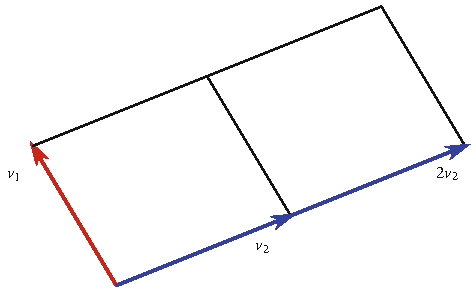
\includegraphics[width=0.564\linewidth]{images/vector/fig-1-11.pdf}
  \caption{把此二维平行六面体一条边的长度加倍，二维体积也加倍}
  \label{fig:1-11}
\end{figure}

我们将用体积的这三条性质来推导一个用 $M=[v_1,v_2,\ldots,v_n]$ 的元素表示 $D$ 的具体公式. 通过推导 $D$ 的具体公式，我们也就证明了 $D$ 既存在又唯一. 当然，$D$ 的这个公式就是你所熟知并喜爱、或者可能深恶痛绝的矩阵行列式公式. 遗憾的是，无法回避的事实是，这个公式既丑得吓人，计算起来又实在麻烦. 但生活（和数学）有时就是这样.

我们首先利用上面的三条性质来确定推导 $D$ 的公式所必需的另外几条性质. 我们要证明的第一件事是那个令人惊讶的事实：体积是带符号的.

\begin{property}{A}\label{prop:1-A}
$D$ 是交替的，即若交换任意两个向量，符号改变：
\[
D(v_1,\ldots,v_i,\ldots,v_j,\ldots,v_n)=-D(v_1,\ldots,v_j,\ldots,v_i,\ldots,v_n).
\]
\end{property}

\begin{proof}
为了使记号简单，我们本可以简单地把它写成 $D(v_i,v_j)=-D(v_j,v_i)$，因为 $v_i$ 与 $v_j$ 是我们关心的仅有的两个向量，其余的保持不变. 下面我们使用这个简化的记号.
\begin{align*}
D(v_i,v_j)&=D(v_i,v_j)+D(v_i,v_i) &&\text{性质 2}\\
&=D(v_i,v_j+v_i) &&\text{性质 3}\\
&=D(v_i,v_j+v_i)-D(v_j+v_i,v_j+v_i) &&\text{性质 2}\\
&=D(-v_j,v_j+v_i) &&\text{性质 3}\\
&=-D(v_j,v_j+v_i) &&\text{性质 3}\\
&=-D(v_j,v_j)-D(v_j,v_i) &&\text{性质 3}\\
&=-D(v_j,v_i) &&\text{性质 2}
\end{align*}
\end{proof}

\begin{property}{B}\label{prop:1-B}
若向量 $v_1,v_2,\ldots,v_n$ 线性相关，则
\[
D(v_1,v_2,\ldots,v_n)=0.
\]
\end{property}

\begin{proof}
由线性相关向量的定义，至少有一个向量可以写成其余向量的线性组合. 不失一般性，假设我们可以写 $v_1=c_2v_2+\cdots+c_nv_n$，其中 $c_i$ 是标量. 反复使用性质 3，我们有
\begin{align*}
D(v_1,v_2,\ldots,v_n)
&=D(c_2v_2+\cdots+c_nv_n,v_2,\ldots,v_n)\\
&=c_2D(v_2,v_2,\ldots,v_n)+c_3D(v_3,v_2,\ldots,v_n)+\cdots+c_nD(v_n,v_2,\ldots,v_n)\\
&=0
\end{align*}
其中最后一个等号来自反复使用性质 2.
\end{proof}

在上面的证明中，``不失一般性''这个短语是什么意思？注意我们假设可以把第一个向量 $v_1$ 写成其余向量的线性组合. 尽管我们在证明中针对 $v_1=c_2v_2+\cdots+c_nv_n$ 这个具体例子做了计算，但如果我们改变假设，决定改为 $v_i=c_1v_1+\cdots+c_{i-1}v_{i-1}+c_{i+1}v_{i+1}+\cdots+c_nv_n$ 对任意 $v_i$ 成立，那么计算将本质相同并给出相同的结果. 当然，我们不会把本质上相同的计算重复 $n$ 遍，那将浪费时间和精力. 数学家的绕行办法是使用``不失一般性''这个短语，然后只对一种具体情况做计算. 大家理解，如果你真的愿意去执行计算，所有其他情况都将完全相同并给出相同的结果.

\begin{property}{C}\label{prop:1-C}
把一个向量的倍数加到另一个向量上不改变行列式.
\end{property}

\begin{proof}
不失一般性，假设我们把 $c$ 倍的 $v_j$ 加到 $v_i$ 上.
\begin{align*}
D(v_1,\ldots,v_i+cv_j,\ldots,v_n)
&=D(v_1,\ldots,v_i,\ldots,v_n)+cD(v_1,\ldots,v_j,\ldots,v_n)\\
&=D(v_1,\ldots,v_i,\ldots,v_n)
\end{align*}
其中最后一个等号来自性质 2，因为向量 $v_j$ 重复出现.
\end{proof}

\begin{question}\label{q:1-13}
解释在性质 C 的证明中``不失一般性''这个短语是如何使用的.
\end{question}

有了这些性质，我们几乎准备好推导行列式的公式了. 为此所需的最后一个要素是置换. 因此我们花一点时间回顾置换. 集合 $\{1,\ldots,n\}$ 的置换是从 $\{1,\ldots,n\}$ 到自身的双射（一一且映上）函数. $\{1,\ldots,n\}$ 的置换集合通常记为 $S_n$. 于是 $S_n$ 的每个元素实际上都是一个置换函数，而 $S_n$ 中有 $n!$ 个元素.

\begin{question}\label{q:1-14}
解释在置换函数的语境中一一与映上是什么意思.
\end{question}

看出 $S_n$ 中有 $n!$ 个元素是相当直接的. 设 $\sigma\in S_n$. 则 $\sigma:\{1,\ldots,n\}\to\{1,\ldots,n\}$. 因此 $\sigma(1)$ 有 $n$ 种可能的选择，即 $\{1,\ldots,n\}$ 中的任意元素. $\sigma(2)$ 可以是 $\{1,\ldots,n\}$ 中除 $\sigma(1)$ 之外的任意元素，因为 $\sigma$ 是一一的，所以它有 $n-1$ 种可能的选择. 类似地，$\sigma(3)$ 可以是 $\{1,\ldots,n\}$ 中除 $\sigma(1)$ 或 $\sigma(2)$ 之外的任意元素，所以有 $n-2$ 种可能的选择. 这样继续下去，直到 $\sigma(n)$ 由剩下的那个元素决定. 总之，$\{1,\ldots,n\}$ 的置换总数为
\[
n\cdot(n-1)\cdot(n-2)\cdot\cdots\cdot1=n!.
\]

我们把一个具体的置换 $\sigma$ 记为
\[
\begin{pmatrix}1&2&\cdots&n\\\downarrow&\downarrow&\cdots&\downarrow\\\sigma(1)&\sigma(2)&\cdots&\sigma(n)\end{pmatrix}.
\]
这种记号称为 Cauchy 两行记号，虽然清楚，但也很笨拙. 只取这个数组的第二行，就得到更简洁的 Cauchy 单行记号，即有序列表 $\bigl(\sigma(1),\sigma(2),\ldots,\sigma(n)\bigr)$. 因此，若 $\sigma\in S_3$，我们写 $(2,1,3)$ 表示
\[
\begin{pmatrix}1&2&3\\\downarrow&\downarrow&\downarrow\\2&1&3\end{pmatrix}.
\]
注意，有些书使用循环记号，其中 $(2,1,3)$ 表示
\[
\begin{pmatrix}1&2&3\\\downarrow&\downarrow&\downarrow\\3&1&2\end{pmatrix}.
\]
也就是说，列表的第一个元素被映到第二个，第二个被映到第三个，最后一个被映到第一个，$2\mapsto1\mapsto3\mapsto2$. 在查阅其他书时要小心，务必弄清它们使用哪种记号. 在循环记号中，上面的 $\sigma$ 可以简单地写为 $(1,2)$，其中把自身映到自身的固定元素 3 不写出来. 然而，在这里我们只使用 Cauchy 单行记号或两行记号.

只交换两个元素的置换称为对换. 我们使用对换的特殊记号：$\tau_{i,j}$ 表示 $i$ 与 $j$ 交换，所有其他元素固定. 我们用一个希望能使想法清楚的例子来说明：对换 $\tau_{3,7}\in S_8$ 由
\[
\begin{pmatrix}1&2&3&4&5&6&7&8\\\downarrow&\downarrow&\downarrow&\downarrow&\downarrow&\downarrow&\downarrow&\downarrow\\1&2&7&4&5&6&3&8\end{pmatrix}
\]
给出.

接下来我们注意到，两个置换的复合仍然是一个置换. 为了这个例子的目的，我们使用 $S_5$，它足够大而不平凡，又足够小而易于处理. 设 $\sigma\in S_5$ 由
\[
\begin{pmatrix}1&2&3&4&5\\\downarrow&\downarrow&\downarrow&\downarrow&\downarrow\\4&3&1&5&2\end{pmatrix}
\]
给出，对换 $\tau_{1,3}\in S_5$ 由
\[
\begin{pmatrix}1&2&3&4&5\\\downarrow&\downarrow&\downarrow&\downarrow&\downarrow\\3&2&1&4&5\end{pmatrix}
\]
给出. 我们把复合 $\tau_{1,3}\circ\sigma$ 写为
\[
\begin{array}{c c c c c c}
\sigma&1&2&3&4&5\\
\downarrow&\downarrow&\downarrow&\downarrow&\downarrow&\downarrow\\
&4&3&1&5&2\\
\tau_{1,3}&\downarrow&\downarrow&\downarrow&\downarrow&\downarrow\\
&4&1&3&5&2
\end{array}
\]
注意由于中间一行不是按升序排列的，这并不完全是 Cauchy 两行记号，但所发生的事应该很清楚. 对换 $\tau_{1,3}$ 用红色标出，以帮助阅读这个图示. 其次，不难看出，可以找到一串对换把任意给定的置换变成恒等置换. 例如，置换 $\tau_{3,4}\circ\tau_{2,4}\circ\tau_{2,3}\circ\tau_{2,5}\circ\tau_{1,4}\circ\tau_{1,3}\circ\sigma$ 是恒等置换：
\[
\begin{array}{c c c c c c}
\sigma&1&2&3&4&5\\
\downarrow&\downarrow&\downarrow&\downarrow&\downarrow&\downarrow\\
&4&3&1&5&2\\
\tau_{1,3}&\downarrow&\downarrow&\downarrow&\downarrow&\downarrow\\
&4&1&3&5&2\\
\tau_{1,4}&\downarrow&\downarrow&\downarrow&\downarrow&\downarrow\\
&1&4&3&5&2\\
\tau_{2,5}&\downarrow&\downarrow&\downarrow&\downarrow&\downarrow\\
&1&4&3&2&5\\
\tau_{2,3}&\downarrow&\downarrow&\downarrow&\downarrow&\downarrow\\
&1&4&2&3&5\\
\tau_{2,4}&\downarrow&\downarrow&\downarrow&\downarrow&\downarrow\\
&1&2&4&3&5\\
\tau_{3,4}&\downarrow&\downarrow&\downarrow&\downarrow&\downarrow\\
&1&2&3&4&5
\end{array}
\]
但注意 $\tau_{4,5}\circ\tau_{3,4}\circ\tau_{2,3}\circ\tau_{1,4}\circ\sigma$，
\[
\begin{array}{c c c c c c}
\sigma&1&2&3&4&5\\
\downarrow&\downarrow&\downarrow&\downarrow&\downarrow&\downarrow\\
&4&3&1&5&2\\
\tau_{1,4}&\downarrow&\downarrow&\downarrow&\downarrow&\downarrow\\
&1&3&4&5&2\\
\tau_{2,3}&\downarrow&\downarrow&\downarrow&\downarrow&\downarrow\\
&1&2&4&5&3\\
\tau_{3,4}&\downarrow&\downarrow&\downarrow&\downarrow&\downarrow\\
&1&2&3&5&4\\
\tau_{4,5}&\downarrow&\downarrow&\downarrow&\downarrow&\downarrow\\
&1&2&3&4&5
\end{array}
\]
也给出恒等置换. $\tau_{2,3}\circ\tau_{1,3}\circ\tau_{4,5}\circ\tau_{2,5}\circ\tau_{2,4}\circ\tau_{4,5}\circ\tau_{1,4}\circ\tau_{2,4}\circ\sigma$ 也是如此，
\[
\begin{array}{c c c c c c}
\sigma&1&2&3&4&5\\
\downarrow&\downarrow&\downarrow&\downarrow&\downarrow&\downarrow\\
&4&3&1&5&2\\
\tau_{3,4}&\downarrow&\downarrow&\downarrow&\downarrow&\downarrow\\
&3&4&1&5&2\\
\tau_{1,4}&\downarrow&\downarrow&\downarrow&\downarrow&\downarrow\\
&3&1&4&5&2\\
\tau_{4,5}&\downarrow&\downarrow&\downarrow&\downarrow&\downarrow\\
&3&1&5&4&2\\
\tau_{2,4}&\downarrow&\downarrow&\downarrow&\downarrow&\downarrow\\
&3&1&5&2&4\\
\tau_{2,5}&\downarrow&\downarrow&\downarrow&\downarrow&\downarrow\\
&3&1&2&5&4\\
\tau_{4,5}&\downarrow&\downarrow&\downarrow&\downarrow&\downarrow\\
&3&1&2&4&5\\
\tau_{1,3}&\downarrow&\downarrow&\downarrow&\downarrow&\downarrow\\
&1&3&2&4&5\\
\tau_{2,3}&\downarrow&\downarrow&\downarrow&\downarrow&\downarrow\\
&1&2&3&4&5
\end{array}
\]
所以显然，把一个置换变成恒等置换所需的对换数目并不是唯一的. 在第一个例子中，把 $\sigma$ 变成恒等置换需要 $6$ 个对换，第二个例子需要 $4$ 个对换，第三个例子需要 $8$ 个对换. 但注意 $6$、$4$ 和 $8$ 都是偶数. 事实证明，奇偶性（偶或奇）是唯一的. 这意味着对任意置换 $\sigma\in S_n$，把该置换变成恒等置换所需的对换数目要么总是偶数，要么总是奇数. 这一点此处不予证明.

置换 $\sigma\in S_n$ 的符号是一个函数 $\mathrm{sgn}:S_n\to\{+1,-1\}$. 若 $\sigma$ 需要偶数个置换，则 $\mathrm{sgn}(\sigma)=+1$；若 $\sigma$ 需要奇数个置换，则 $\mathrm{sgn}(\sigma)=-1$. 你应该知道有时也使用记号 $\mathrm{sgn}(\sigma)\equiv(-1)^\sigma$. 这个记号背后的想法是：当 $\sigma$ 需要偶数个对换时 $(-1)^{\text{偶}}=1$，当 $\sigma$ 需要奇数个对换时 $(-1)^{\text{奇}}=-1$.

现在，有了置换记号在手，我们可以迈出推导行列式公式的下一步. 假设我们有单位向量
\[
e_1=\begin{bmatrix}1\\0\\\vdots\\0\end{bmatrix},\qquad
e_2=\begin{bmatrix}0\\1\\\vdots\\0\end{bmatrix},\qquad\cdots,\qquad
e_n=\begin{bmatrix}0\\0\\\vdots\\1\end{bmatrix}\in\mathbb{R}^n,
\]
则 $[e_1\,e_2\,\cdots\,e_n]$ 是单位矩阵 $I$，由性质 1 有 $D\bigl([e_1\,e_2\,\cdots\,e_n]\bigr)=D(I)=1$. 其次，若 $\sigma\in S_n$，则它定义单位向量的一个置换，因此 $e_{\sigma(i)}$ 是在第 $\sigma(i)$ 行有 1、其余各处为 0 的向量. 于是我们可以定义矩阵 $E_\sigma=[e_{\sigma(1)}\,e_{\sigma(2)}\,\cdots\,e_{\sigma(n)}]$. 现在证明下面的性质.

\begin{property}{D}\label{prop:1-D}
$D\bigl(E_\sigma\bigr)=\mathrm{sgn}(\sigma)$.
\end{property}

\begin{proof}
注意 $E_\sigma=[e_{\sigma(1)}\,e_{\sigma(2)}\,\cdots\,e_{\sigma(n)}]$ 与 $\sigma$ 的 Cauchy 单行记号 $\bigl(\sigma(1),\sigma(2),\ldots,\sigma(n)\bigr)$ 之间的相似性. 把 $\bigl(\sigma(1),\sigma(2),\ldots,\sigma(n)\bigr)$ 变成恒等置换 $(1,2,\ldots,n)$ 的一串变换，也会把 $E_\sigma=[e_{\sigma(1)}\,e_{\sigma(2)}\,\cdots\,e_{\sigma(n)}]$ 变成单位矩阵 $I$. 由性质 A，每次交换列都会带来因子 $(-1)$. 由于 $\mathrm{sgn}(\sigma)$ 记录把 $\sigma$ 变成恒等置换所需对换的奇偶性，它也就是把 $E_\sigma$ 变成单位矩阵 $I$ 所需列变换的奇偶性，所以我们有 $D(E_\sigma)=\mathrm{sgn}(\sigma)D(I)=\mathrm{sgn}(\sigma)$.
\end{proof}

现在我们拥有了求由 $n$ 个向量张成的平行六面体体积公式所需的全部要素. 当这些向量写成矩阵的列时，这个体积公式正是矩阵的行列式，因此记为 $D$. 首先令
\[
v_1=\begin{bmatrix}a_{11}\\a_{21}\\a_{31}\\\vdots\\a_{n1}\end{bmatrix},\qquad
v_2=\begin{bmatrix}a_{12}\\a_{22}\\a_{32}\\\vdots\\a_{n2}\end{bmatrix},\qquad\cdots,\qquad
v_n=\begin{bmatrix}a_{1n}\\a_{2n}\\a_{3n}\\\vdots\\a_{nn}\end{bmatrix}\in\mathbb{R}^n.
\]
我们想求由 $v_1,v_2,\ldots,v_n$ 张成的平行六面体的体积，也就是以这些向量为列的矩阵的行列式.
\begin{align*}
D\left(\begin{bmatrix}a_{11}&a_{12}&\cdots&a_{1n}\\a_{21}&a_{22}&\cdots&a_{2n}\\\vdots&\vdots&\ddots&\vdots\\a_{n1}&a_{n2}&\cdots&a_{nn}\end{bmatrix}\right)
&=\sum_{i_1=1}^{n}a_{i_11}D\left(\begin{bmatrix}|&a_{12}&\cdots&a_{1n}\\e_{i_1}&a_{22}&\cdots&a_{2n}\\\vdots&\vdots&\ddots&\vdots\\|&a_{n2}&\cdots&a_{nn}\end{bmatrix}\right)\\
&=\sum_{i_1,i_2=1}^{n}a_{i_11}a_{i_22}D\left(\begin{bmatrix}|&|&a_{13}&\cdots&a_{1n}\\e_{i_1}&e_{i_2}&a_{23}&\cdots&a_{2n}\\\vdots&\vdots&\vdots&\ddots&\vdots\\|&|&a_{n3}&\cdots&a_{nn}\end{bmatrix}\right)\\
&=\cdots\\
&=\sum_{i_1,i_2,\ldots,i_n=1}^{n}a_{i_11}a_{i_22}\cdots a_{i_nn}
  D\left(\begin{bmatrix}|&|&&|\\e_{i_1}&e_{i_2}&\cdots&e_{i_n}\\\vdots&\vdots&&\vdots\\|&|&&|\end{bmatrix}\right)\\
&=\sum_{\sigma\in S_n}a_{\sigma(1)1}a_{\sigma(2)2}\cdots a_{\sigma(n)n}
  D\left(\begin{bmatrix}|&|&&|\\e_{\sigma(1)}&e_{\sigma(2)}&\cdots&e_{\sigma(n)}\\\vdots&\vdots&&\vdots\\|&|&&|\end{bmatrix}\right)\\
&=\sum_{\sigma\in S_n}a_{\sigma(1)1}a_{\sigma(2)2}\cdots a_{\sigma(n)n}\,\mathrm{sgn}(\sigma)\\
&=\sum_{\sigma\in S_n}\mathrm{sgn}(\sigma)\prod_{i=1}^{n}a_{\sigma(i)i}
\end{align*}
注意从第一个到第 $n$ 个等号都使用了性质 D. 在第四步中，当某个 $e_{i_j}=e_{i_k}$（对某些 $i_j,i_k$）时行列式为零，所以非零项恰是 $e_{i_1},\ldots,e_{i_n}$ 为 $\{1,\ldots,n\}$ 的某个置换 $\sigma$ 的那些项. 于是我们得到矩阵行列式的标准公式：

\begin{center}
\textbf{矩阵的行列式公式：}
\end{center}
\[
\begin{vmatrix}a_{11}&a_{12}&\cdots&a_{1n}\\a_{21}&a_{22}&\cdots&a_{2n}\\\vdots&\vdots&\ddots&\vdots\\a_{n1}&a_{n2}&\cdots&a_{nn}\end{vmatrix}
=\sum_{\sigma\in S_n}\mathrm{sgn}(\sigma)\prod_{i=1}^{n}a_{\sigma(i)i}.
\]

注意这里我们使用了矩阵记号的一个小变体：数组两侧用竖直线 $|$ 而不是方括号 $[$ 或 $]$ 来表示矩阵的行列式.

我们要重申，这个行列式公式完全建立在我们关于由 $n$ 个向量生成的 $n$ 平行六面体的体积应当如何的三种直觉观念之上（外加一点置换记号以及知道置换奇偶性是唯一的）. 通过实际推导这个公式，我们证明了存在唯一一个满足性质 1--3 的公式.

\begin{question}\label{q:1-15}
我们的行列式公式当然应当满足我们用来推导公式的那三条原始性质. 用推导出的行列式公式证明：
\begin{enumerate}
  \item[(a)] $D(I)=1$，
  \item[(b)] 若任意两列相同，则 $D(A)=0$，
  \item[(c)] 若固定 $n-1$ 列，则 $D$ 是剩余一列的线性函数.
\end{enumerate}
\end{question}

矩阵 $A$ 的转置，记为 $A^T$，是通过``沿对角线反射''得到的. 也就是说，$A$ 的第一列变成 $A^T$ 的第一行，$A$ 的第二列变成 $A^T$ 的第二行，依此类推. 例如，若
\[
A=\begin{bmatrix}1&4&7\\2&5&8\\3&6&9\end{bmatrix},\qquad\text{则}\qquad
A^T=\begin{bmatrix}1&2&3\\4&5&6\\7&8&9\end{bmatrix}.
\]

\begin{question}\label{q:1-16}
利用上面推导的 $D$ 的公式，证明 $D(A)=D(A^T)$.
\end{question}

\begin{question}\label{q:1-17}
性质 1--3 与 A--D 都是针对列陈述的. 由于 $A$ 的列变成 $A^T$ 的行且 $D(A)=D(A^T)$，所有这些性质都可以改写为针对行而非列. 把性质 1--3 与 A--D 改写为针对行而非列.
\end{question}

\section{多元函数的导数}

在本节中我们将引入多元函数导数的概念. 你可能在多元微积分课程中见过其中一些思想，不过这些思想的完整引入通常发生在初等分析课程中. 这里我们只提供本书所必需的要点.

回顾一下，若你有一个函数 $f:\mathbb{R}\to\mathbb{R}$，则 $f$ 在点 $x_0\in\mathbb{R}$ 处的导数（记为 $f'(x)$）由
\[
f'(x_0)=\lim_{h\to0}\frac{f(x_0+h)-f(x_0)}{h}
\]
给出，如果该极限存在的话. 但注意
\begin{align*}
f'(x_0)&=\lim_{h\to0}\frac{f(x_0+h)-f(x_0)}{h}\\
&\Rightarrow\quad\lim_{h\to0}\frac{f(x_0+h)-f(x_0)-f'(x_0)h}{h}=0\\
&\Rightarrow\quad\lim_{x\to x_0}\frac{f(x)-f(x_0)-f'(x_0)(x-x_0)}{x-x_0}=0\\
&\Rightarrow\quad\lim_{x\to x_0}\frac{|f(x)-f(x_0)-f'(x_0)(x-x_0)|}{|x-x_0|}=0.
\end{align*}
由于 $f'(x_0)$ 表示 $f$ 的图像在点 $(x_0,f(x_0))$ 处切线的斜率，$f$ 在点 $x_0$ 处可微意味着存在一个数 $m$ 使得
\[
\lim_{x\to x_0}\frac{|f(x)-f(x_0)-m(x-x_0)|}{|x-x_0|}=0.
\]

\begin{figure}[htbp]
  \centering
  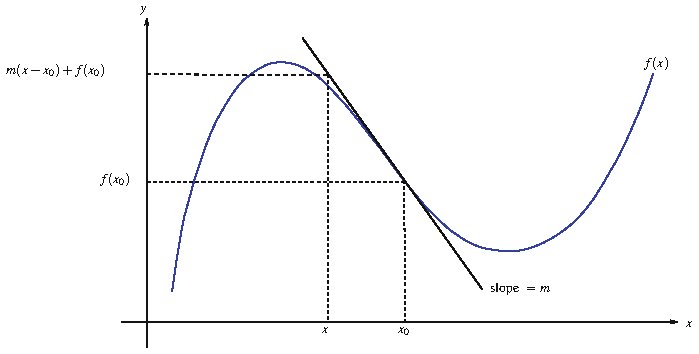
\includegraphics[width=0.943\linewidth]{images/vector/fig-1-12.pdf}
  \caption{函数 $f$ 在点 $x_0$ 处的线性逼近}
  \label{fig:1-12}
\end{figure}

现在我们想考虑上面表达式中 $m(x-x_0)$ 这一部分. 显然 $x-x_0$ 只是某个数，我们把它叫做 $s$. 然后考虑函数 $T:\mathbb{R}\to\mathbb{R}$，其中 $T(s)=ms$. 由于
\[
T(s+t)=m(s+t)=ms+mt=T(s)+T(t)
\qquad\text{且}\qquad
T(cs)=m(cs)=c(ms)=cT(s),
\]
故 $T$ 是一个线性函数，即线性变换. 事实上，$T$ 是在点 $(x_0,f(x_0))$ 处最接近逼近函数 $f$ 的线性函数，见图 \ref{fig:1-12}. 通常，为了简单起见，我们就说 $T$ 是 $f$ 在 $x_0$ 处最接近的线性逼近. 所以对非常接近 $x_0$ 的 $x$ 值，我们有
\[
f(x)\approx\underbrace{m(x-x_0)}_{\text{$f$ 在 $x_0$ 处的线性逼近}}\;+\;\underbrace{f(x_0)}_{\text{把线性逼近上下平移适当量}}.
\]

我们现在要做的是把导数的概念推广到形如 $f:\mathbb{R}^n\to\mathbb{R}^m$ 的函数. 我们假定函数 $f$ 具有形式
\[
f(x_1,x_2,\ldots,x_n)=\bigl(f_1(x_1,x_2,\ldots,x_n),f_2(x_1,x_2,\ldots,x_n),\ldots,f_m(x_1,x_2,\ldots,x_n)\bigr).
\]
我们想找到最接近逼近这个函数 $f:\mathbb{R}^n\to\mathbb{R}^m$ 的线性变换，记为 $Df$，在某个具体的点 $x_0=(x_{10},x_{20},\ldots,x_{n0})\in\mathbb{R}^n$ 处. 若 $f$ 在 $x_0\in\mathbb{R}^n$ 处可微，则存在线性变换 $Df(x_0):\mathbb{R}^n\to\mathbb{R}^m$ 使得
\[
\lim_{x\to x_0}\frac{\|f(x)-f(x_0)-Df(x_0)(x-x_0)\|}{\|x-x_0\|}=0.
\]
这里 $Df(x_0)$ 是一个线性映射，$(x-x_0)$ 是 $\mathbb{R}^n$ 中起点在 $x_0$、终点在 $x$ 的向量，而 $Df(x_0)(x-x_0)$ 是该线性映射作用在向量上的结果，它是 $\mathbb{R}^m$ 中的一个元素. 若 $h$ 是 $\mathbb{R}^n$ 中的向量，有时我们写 $Df(x_0)\cdot h$ 而不是 $Df(x_0)(h)$.

关于 $\|\cdot\|$ 是什么以及为什么需要它，简单说几句. $\|\cdot\|$ 表示称为欧几里得范数的对象，本质上它是绝对值 $|\cdot|$ 的多维版本. 给定向量
\[
v=\begin{bmatrix}x_1\\\vdots\\x_n\end{bmatrix},\qquad\text{则}\qquad
\|v\|=\sqrt{\sum_{i=1}^{n}x_i^2},
\]
这只是向量的长度. 如果你把向量 $v$ 想成点 $(x_0,\ldots,x_n)$，这给出该点到原点的距离. 没有范数，我们定义中的分子和分母都将是 $\mathbb{R}^m$ 中的点或向量（取决于你如何看待它们），而人们不能用一个点或向量除以另一个点或向量. 范数使我们能够简单地相除两个数.

很容易有点糊涂. 记号可能有点歧义. 但通常一点点歧义能带来很大的灵活性，所以这种歧义被容忍，甚至被拥抱. 注意 $Df$、$Df(x)$ 和 $Df(x_0)$ 都用来表示作为函数 $f$ 的逼近的线性变换. 如果我们在泛泛地谈，还没有实际选定具体的基点 $x_0$，那么我们使用 $Df$ 或 $Df(x)$. 如果我们选定了基点 $x_0$，那么我们使用 $Df(x_0)$. 这与说 $f(x)=x^2$ 的导数是 $f'$ 或 $f'(x)$（两者都是 $2x$），而 $f$ 在点 $x_0=3$ 处的导数是 $f'(3)=6$ 非常类似. 此外，画出精确的图像不再可能. 要画出 $f:\mathbb{R}^n\to\mathbb{R}^m$ 的图像，实际上需要画出 $\mathbb{R}^{n+m}$. 我们画的图像当然类似，但必须认识到它实际上是一幅漫画，如图 \ref{fig:1-13} 所示.

\begin{figure}[htbp]
  \centering
  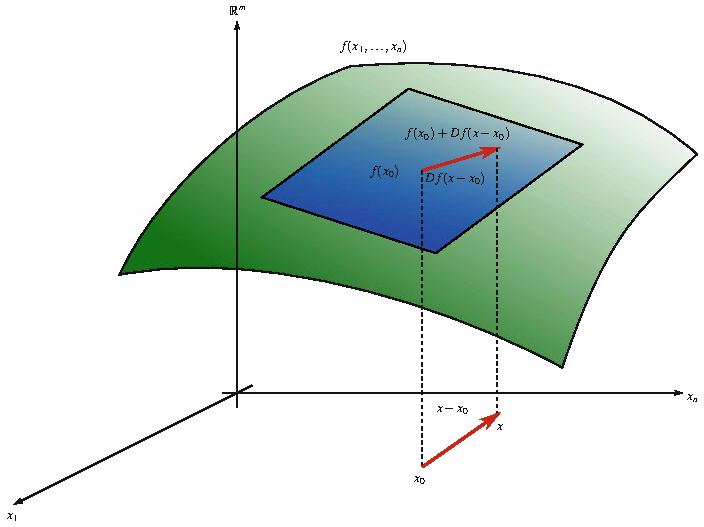
\includegraphics[width=0.960\linewidth]{images/vector/fig-1-13.pdf}
  \caption{函数 $f$ 在点 $x_0$ 处的线性逼近，以三维方式描绘}
  \label{fig:1-13}
\end{figure}

和之前一样，我们有
\[
f(x)\approx\underbrace{Df(x_0)(x-x_0)}_{\text{$f$ 在 $x_0$ 处的线性逼近}}\;+\;\underbrace{f(x_0)}_{\text{把线性逼近适当平移}}.
\]

我们之前看到可以把线性变换写成矩阵，所以我们的目标是把 $Df(x)$ 写成一个矩阵. 使用与之前相同的记号，并假定 $\mathbb{R}^n$ 的基由 $e_j$ 给出、$\mathbb{R}^m$ 的基由 $\tilde{e}_i$ 给出，我们想找到满足下式的 $a_{ij}$：
\[
Df(x)\cdot e_j=\sum_{i=1}^{m}a_{ij}\tilde{e}_i=\begin{bmatrix}a_{1j}\\a_{2j}\\\vdots\\a_{mj}\end{bmatrix}.
\]
换句话说，$Df(x)$ 的第 $j$ 列的第 $i$ 个分量就是 $Df(x)\cdot e_j$ 的第 $i$ 个分量.

为了求 $Df(x)$ 的矩阵表示，回想向量微积分中的结论：给定函数 $f:\mathbb{R}^n\to\mathbb{R}$，我们把 $f$ 关于 $x_j$ 的偏导数定义为
\[
\frac{\partial f}{\partial x_j}=\lim_{h\to0}\frac{f(x_1,\ldots,x_j+h,\ldots,x_n)-f(x_1,\ldots,x_j,\ldots,x_n)}{h}.
\]
当我们给定一个函数
\[
f:\mathbb{R}^n\to\mathbb{R}^m,\qquad
(x_1,\ldots,x_n)\longmapsto\bigl(f_1(x_1,\ldots,x_n),\ldots,f_m(x_1,\ldots,x_n)\bigr)
\]
时，我们当然可以对每个 $f_i$（$1\leq i\leq m$）关于每个 $x_j$（$1\leq j\leq n$）求偏导数，
\[
\frac{\partial f_i}{\partial x_j}=\lim_{h\to0}\frac{f_i(x_1,\ldots,x_j+h,\ldots,x_n)-f_i(x_1,\ldots,x_j,\ldots,x_n)}{h}.
\]
这里有几件事要注意. 首先，$x_j$ 是对应于 $\mathbb{R}^n$ 中基向量 $e_j$ 的坐标，而 $f_i(x_1,\ldots,x_n)\equiv f_i$ 是对应于 $\mathbb{R}^m$ 中基向量 $\tilde{e}_i$ 的坐标. 其次，我们保持 $x_1,\ldots,x_{j-1},x_{j+1},\ldots,x_n$ 固定，只让 $x_j$ 变化. 固定这些变量后的函数 $f_i$ 成为从 $\mathbb{R}$ 到 $\mathbb{R}$ 的函数，因此它最接近的线性逼近只是一个表示斜率的数，记为 $a_{ij}$. 于是我们有
\[
\frac{\partial f_i}{\partial x_j}=a_{ij}.
\]

考虑我们对 $Df(x_0)$ 的定义，即它是满足
\[
\lim_{x\to x_0}\frac{\|f(x)-f(x_0)-Df(x_0)(x-x_0)\|}{\|x-x_0\|}=0
\]
的线性变换，其中 $Df(x_0)(x-x_0)$ 是 $\mathbb{R}^m$ 中的列向量，而 $x-x_0$ 是 $\mathbb{R}^n$ 中的向量.

为了求 $Df(x_0)$ 的 $a_{ij}$，我们需要求 $Df(x_0)\cdot e_j$ 的第 $i$ 个元素. 令
\[
x=\begin{bmatrix}x_{10}\\x_{20}\\\vdots\\x_{n0}\end{bmatrix}+h\begin{bmatrix}0\\\vdots\\1\\\vdots\\0\end{bmatrix}=x_0+he_j,
\]
我们可以把上面的式子写为
\begin{align*}
\lim_{x\to x_0}\frac{\|f(x)-f(x_0)-Df(x_0)(he_j)\|}{\|he_j\|}&=0\\
\Rightarrow\quad\lim_{h\to0}\frac{\left\|\begin{aligned}
&f(x_{10},\ldots,x_{i0}+h,\ldots,x_{n0})\\
&\quad-f(x_{10},\ldots,x_{i0},\ldots,x_{n0})\\
&\quad-hDf(x_0)\cdot e_j
\end{aligned}\right\|}{|h|}&=0.
\end{align*}
这个表达式的分子是 $\mathbb{R}^m$ 中的一个向量，其第 $i$ 个分量通过看函数 $f$ 定义中的 $f_i$ 得到. 于是 $Df(x_0)$ 的第 $j$ 列的第 $i$ 个分量由下式给出：
\begin{align*}
\lim_{h\to0}\frac{\left|\begin{aligned}
&f_i(x_{10},\ldots,x_{i0}+h,\ldots,x_{n0})\\
&\quad-f_i(x_{10},\ldots,x_{i0},\ldots,x_{n0})\\
&\quad-ha_{ij}
\end{aligned}\right|}{|h|}&=0\\
\Rightarrow\quad a_{ij}&=\lim_{h\to0}\frac{\begin{aligned}
f_i(x_{10},\ldots,x_{i0}+h,\ldots,x_{n0})\\
-f_i(x_{10},\ldots,x_{i0},\ldots,x_{n0})
\end{aligned}}{h}
\end{align*}
但这恰恰就是 $\frac{\partial f_i}{\partial x_j}$. 因此，$Df(x)$ 的矩阵表示由一个称为 $f$ 的 \newterm{jacobian-matrix}{Jacobian 矩阵}{Jacobian matrix} 的矩阵给出：
\[
Df(x)=\begin{bmatrix}
\frac{\partial f_1}{\partial x_1}&\frac{\partial f_1}{\partial x_2}&\cdots&\frac{\partial f_1}{\partial x_n}\\[2mm]
\frac{\partial f_2}{\partial x_1}&\frac{\partial f_2}{\partial x_2}&\cdots&\frac{\partial f_2}{\partial x_n}\\
\vdots&\vdots&\ddots&\vdots\\
\frac{\partial f_m}{\partial x_1}&\frac{\partial f_m}{\partial x_2}&\cdots&\frac{\partial f_m}{\partial x_n}
\end{bmatrix}
=\left(\frac{\partial f_i}{\partial x_j}\right)_{\substack{i=\text{行}\\j=\text{列}}}.
\]

\section{小结、参考文献与问题}

\subsection{小结}

每章的小结包含该章所涵盖的最重要的概念与公式，以及必要的结束语. 小结一节的用意是既作为快速参考，也作为章节复习.

向量空间是一个集合 $V$，配备加法 $+$ 与标量乘法 $\cdot$、加法单位元 $0$，以及一个``取负运算''，并满足以下八条公理. 给定向量空间元素 $u,v,w\in V$ 和标量 $c,d\in\mathbb{R}$，这八条公理是
\begin{enumerate}
  \item $v+w=w+v$
  \item $(u+v)+w=u+(v+w)$
  \item $v+0=v=0+v$
  \item $v+(-v)=0$
  \item $1\cdot v=v$
  \item $c\cdot(d\cdot v)=(c\cdot d)\cdot v$
  \item $c\cdot(v+w)=c\cdot v+c\cdot w$
  \item $(c+d)\cdot v=c\cdot v+d\cdot v
  $
\end{enumerate}
向量空间最重要的例子是 $\mathbb{R}^n$. $\mathbb{R}^n$ 的元素写成列向量. 向量空间 $V$ 的基是满足线性无关且张成该向量空间的元素集 $\{v_1,\ldots,v_n\}$. 线性泛函 $T:\mathbb{R}^n\to\mathbb{R}$ 是具有以下两条性质的映射：
\begin{enumerate}
  \item $T(v+w)=T(v)+T(w)$
  \item $T(c\cdot v)=c\cdot T(v)$
\end{enumerate}
其中 $v,w\in\mathbb{R}^n$，$c\in\mathbb{R}$. $\mathbb{R}^n$ 的对偶空间是 $\mathbb{R}^n$ 上所有线性泛函的集合，即所有满足这两条性质的映射 $T:\mathbb{R}^n\to\mathbb{R}$. $\mathbb{R}^n$ 的对偶空间记为 $(\mathbb{R}^n)^*$. 向量空间 $V$ 的任意一组基都诱导出 $V^*$ 的一组对偶基.

利用我们期望平行六面体体积如何表现的三条性质，我们发现体积天然带有符号. 此外，利用这些性质我们能够推导出矩阵行列式的公式，它求以矩阵的列为边的平行六面体的有向体积.

\begin{center}
\textbf{矩阵的行列式公式：}
\end{center}
\[
\begin{vmatrix}a_{11}&a_{12}&\cdots&a_{1n}\\a_{21}&a_{22}&\cdots&a_{2n}\\\vdots&\vdots&\ddots&\vdots\\a_{n1}&a_{n2}&\cdots&a_{nn}\end{vmatrix}
=\sum_{\sigma\in S_n}\mathrm{sgn}(\sigma)\prod_{i=1}^{n}a_{\sigma(i)i}.
\]

最后，给定由 $f=(f_1,\ldots,f_m)$ 定义的函数 $f:\mathbb{R}^n\to\mathbb{R}^m$，该函数的导数 $Df$ 是由 Jacobian 矩阵给出的线性变换
\[
Df(x)=\begin{bmatrix}
\frac{\partial f_1}{\partial x_1}&\frac{\partial f_1}{\partial x_2}&\cdots&\frac{\partial f_1}{\partial x_n}\\[2mm]
\frac{\partial f_2}{\partial x_1}&\frac{\partial f_2}{\partial x_2}&\cdots&\frac{\partial f_2}{\partial x_n}\\
\vdots&\vdots&\ddots&\vdots\\
\frac{\partial f_m}{\partial x_1}&\frac{\partial f_m}{\partial x_2}&\cdots&\frac{\partial f_m}{\partial x_n}
\end{bmatrix}
=\left(\frac{\partial f_i}{\partial x_j}\right)_{\substack{i=\text{行}\\j=\text{列}}}.
\]

\subsection{参考文献与进一步阅读}

本章所呈现的材料都是相当标准的，不过呈现材料所采用的具体方式与本书其余部分的要求一致. 关于线性代数的书不胜枚举，但 Friedberg、Insel 与 Spence 的著作~\cite{ref22} 是一本很好的参考书. 行列式与平行六面体体积的关系也是标准材料，但这里的介绍大体上遵循了一份很好的匿名且未注明日期的关于行列式的讲解~\cite{ref02}. 另见 Abraham、Marsden 与 Ratiu 的著作~\cite{ref01}. 就多元微积分而言，Stewart 的教科书~\cite{ref43} 是一本标准教材. 对于多元微积分稍许更详细的数学介绍，Marsden 与 Hoffman 的书~\cite{ref31} 非常好. 特别是，Marsden 倾向于使用一些出色的记号，本书大部分内容都使用了这些记号.

\subsection{问题}

\begin{question}\label{q:1-18}
令 $V=\{(x_1,x_2)\mid x_1,x_2\in\mathbb{R}\}$. 也就是说，$V$ 是实数有序对的集合. 若 $(a_1,a_2),(b_1,b_2)\in V$ 且 $c\in\mathbb{R}$ 是标量，定义
\[
(a_1,a_2)+(b_1,b_2)=(a_1+b_1,a_2b_2),\qquad c(a_1,a_2)=(ca_1,a_2).
\]
在这些运算下 $V$ 是向量空间吗？
\end{question}

\begin{question}\label{q:1-19}
令 $V=\{(x_1,x_2)\mid x_1,x_2\in\mathbb{R}\}$. 若 $(a_1,a_2),(b_1,b_2)\in V$ 且 $c\in\mathbb{R}$ 是标量，定义
\[
(a_1,a_2)+(b_1,b_2)=(a_1+b_1,a_2+b_2),\qquad c(a_1,a_2)=(a_1,0).
\]
在这些运算下 $V$ 是向量空间吗？
\end{question}

\begin{question}\label{q:1-20}
令 $V=\{(x_1,x_2)\mid x_1,x_2\in\mathbb{R}\}$. 若 $(a_1,a_2),(b_1,b_2)\in V$ 且 $c\in\mathbb{R}$ 是标量，定义
\[
(a_1,a_2)+(b_1,b_2)=(a_1+3b_1,a_2+5b_2),\qquad c(a_1,a_2)=(ca_1,ca_2).
\]
在这些运算下 $V$ 是向量空间吗？
\end{question}

\begin{question}\label{q:1-21}
令 $V=\{(x_1,x_2)\mid x_1,x_2\in\mathbb{R}\}$. 若 $(a_1,a_2),(b_1,b_2)\in V$ 且 $c\in\mathbb{R}$ 是标量，定义
\[
(a_1,a_2)+(b_1,b_2)=(a_1+b_1,a_2+b_2),\qquad
c(a_1,a_2)=\begin{cases}(0,0)&c=0\\\left(ca_1,\frac{a_2}{c}\right)&c\neq0.\end{cases}
\]
在这些运算下 $V$ 是向量空间吗？
\end{question}

\begin{question}\label{q:1-22}
设 $V$、$W$ 是向量空间，令 $Z=\{(v,w)\mid v\in V,\,w\in W\}$. 若 $(v_1,w_1)$、$(v_2,w_2)\in Z$，且 $c\in\mathbb{R}$ 是标量，定义
\[
(v_1,w_1)+(v_2,w_2)=(v_1+v_2,w_1+w_2),
\]
且
\[
c(v_1,w_1)=(cv_1,cw_1).
\]
证明 $Z$ 是向量空间.
\end{question}

\begin{question}\label{q:1-23}
考虑向量
\[
v_1=\begin{bmatrix}1\\3\\-4\\2\end{bmatrix},\qquad
v_2=\begin{bmatrix}1\\1\\-2\\0\end{bmatrix},\qquad
v_3=\begin{bmatrix}1\\-3\\2\\-4\end{bmatrix},\qquad
v_4=\begin{bmatrix}-2\\0\\2\\0\end{bmatrix}.
\]
证明这些向量线性相关. 也就是说，找到不全为零的标量 $c_1,c_2,c_3,c_4$，使得
\[
c_1v_1+c_2v_2+c_3v_3+c_4v_4=\begin{bmatrix}0\\0\\0\\0\end{bmatrix}.
\]
\end{question}

\begin{question}\label{q:1-24}
考虑向量
\[
v_1=\begin{bmatrix}1\\0\\0\\-1\end{bmatrix},\qquad
v_2=\begin{bmatrix}0\\1\\0\\-1\end{bmatrix},\qquad
v_3=\begin{bmatrix}0\\0\\1\\-1\end{bmatrix},\qquad
v_4=\begin{bmatrix}0\\0\\0\\1\end{bmatrix}.
\]
证明这些向量线性无关. 为此证明：使得
\[
c_1v_1+c_2v_2+c_3v_3+c_4v_4=\begin{bmatrix}0\\0\\0\\0\end{bmatrix}
\]
成立的唯一线性组合是其中所有标量 $c_1,c_2,c_3,c_4$ 都为零的那一个.
\end{question}

\begin{question}\label{q:1-25}
给出 $\mathbb{R}^3$ 中三个线性相关向量的集合，使得其中任何一个向量都不是其余向量中另一个的倍数.
\end{question}

\begin{question}\label{q:1-26}
给出 $\mathbb{R}^4$ 中四个线性相关向量的集合，使得其中任何一个向量都不是其余向量中另一个的倍数.
\end{question}

\begin{question}\label{q:1-27}
向量 $v_1=\begin{bmatrix}1\\1\end{bmatrix}$、$v_2=\begin{bmatrix}1\\-2\end{bmatrix}$ 张成 $\mathbb{R}^2$ 吗？也就是说，对任意向量 $v\in\mathbb{R}^2$，能否找到标量 $c_1,c_2$ 使得 $c_1v_1+c_2v_2=v$？
\end{question}

\begin{question}\label{q:1-28}
向量 $v_1=\begin{bmatrix}1\\1\\0\end{bmatrix}$、$v_2=\begin{bmatrix}0\\1\\1\end{bmatrix}$、$v_3=\begin{bmatrix}1\\0\\1\end{bmatrix}$ 张成 $\mathbb{R}^3$ 吗？也就是说，对任意向量 $v\in\mathbb{R}^3$，能否找到标量 $c_1,c_2,c_3$ 使得 $c_1v_1+c_2v_2+c_3v_3=v$？
\end{question}

\begin{question}\label{q:1-29}
向量 $v_1=\begin{bmatrix}4\\2\\0\end{bmatrix}$、$v_2=\begin{bmatrix}0\\1\\1\end{bmatrix}$、$v_3=\begin{bmatrix}2\\2\\1\end{bmatrix}$ 张成 $\mathbb{R}^3$ 吗？也就是说，对任意向量 $v\in\mathbb{R}^3$，能否找到标量 $c_1,c_2,c_3$ 使得 $c_1v_1+c_2v_2+c_3v_3=v$？
\end{question}

\begin{question}\label{q:1-30}
若 $T:V\to W$ 是线性变换，证明 $T(\mathbf{0}_V)=\mathbf{0}_W$，其中 $\mathbf{0}_V$ 是 $V$ 中的零向量，$\mathbf{0}_W$ 是 $W$ 中的零向量.
\end{question}

\begin{question}\label{q:1-31}
若 $T:V\to W$ 是线性变换，证明 $T(cx+y)=cT(x)+T(y)$.
\end{question}

\begin{question}\label{q:1-32}
若 $T:V\to W$ 是线性变换，证明
\[
T\left(\sum_{i=1}^{n}a_iv_i\right)=\sum_{i=1}^{n}c_iT(v_i).
\]
\end{question}

\begin{question}\label{q:1-33}
定义 $T:\mathbb{R}^2\to\mathbb{R}^2$ 为
\[
T\binom{x_1}{x_2}=\binom{2x_1+x_2}{x_1}.
\]
$T$ 是线性变换吗？如果是，求 $T$ 的矩阵表示.
\end{question}

\begin{question}\label{q:1-34}
对任意角度 $\theta$，定义 $T_\theta:\mathbb{R}^2\to\mathbb{R}^2$ 为
\[
T_\theta\binom{x_1}{x_2}=\binom{x_1\cos\theta-x_2\sin\theta}{x_1\sin\theta+x_2\cos\theta}.
\]
证明 $T_\theta$ 是线性变换. 变换 $T_\theta$ 称为绕 $\theta$ 角的旋转. 求 $T_\theta$ 的矩阵表示.
\end{question}

\begin{question}\label{q:1-35}
定义 $T:\mathbb{R}^2\to\mathbb{R}^2$ 为
\[
T\binom{x_1}{x_2}=\binom{x_1}{-x_2}.
\]
证明 $T$ 是线性变换. 变换 $T$ 称为关于 $x$ 轴的反射. 求 $T$ 的矩阵表示.
\end{question}

\begin{question}\label{q:1-36}
令
\[
\left\{\begin{bmatrix}2\\1\end{bmatrix},\begin{bmatrix}3\\1\end{bmatrix}\right\}
\]
为 $\mathbb{R}^2$ 的一组基. 求对偶基. 也就是说，求与这组基对偶的 $(\mathbb{R}^2)^*$ 的基.
\end{question}

\begin{question}\label{q:1-37}
利用行列式公式，求常数 $C$ 使得
\[
\begin{vmatrix}2a_1&2a_2&2a_3\\3b_1+4c_1&3b_2+4c_2&3b_3+4c_3\\5c_1&5c_2&5c_3\end{vmatrix}
=C\begin{vmatrix}a_1&a_2&a_3\\b_1&b_2&b_3\\c_1&c_2&c_3\end{vmatrix}.
\]
\end{question}

\begin{question}\label{q:1-38}
令
\[
\left\{\begin{bmatrix}1\\0\\1\end{bmatrix},\begin{bmatrix}1\\2\\1\end{bmatrix},\begin{bmatrix}0\\0\\1\end{bmatrix}\right\}
\]
为 $\mathbb{R}^3$ 的一组基. 求对偶基.
\end{question}

\begin{question}\label{q:1-39}
利用行列式公式，求常数 $C$ 使得
\[
\begin{vmatrix}3a_1&3a_2&3a_3\\3b_1&3b_2&3b_3\\3c_1&3c_2&3c_3\end{vmatrix}
=C\begin{vmatrix}a_1&a_2&a_3\\b_1&b_2&b_3\\c_1&c_2&c_3\end{vmatrix}.
\]
\end{question}

\begin{question}\label{q:1-40}
求下列矩阵的行列式的值：
\[
\begin{bmatrix}2&-6\\-2&5\end{bmatrix},\qquad
\begin{bmatrix}3&0&5\\-2&-1&4\\7&6&0\end{bmatrix},\qquad
\begin{bmatrix}0&1&3\\-1&0&-3\\2&3&0\end{bmatrix}.
\]
\end{question}

\begin{question}\label{q:1-41}
求下列函数的 Jacobian 矩阵：
\begin{enumerate}
  \item[(a)] $f(x,y)=xy$
  \item[(b)] $f(x,y)=\sin(x^3+y^2)$
  \item[(c)] $f(x,y,z)=x^5+y^4$
  \item[(d)] $f(x,y)=\bigl(\sin(x\sin(y)),(x+y)^2\bigr)$
  \item[(e)] $f(x,y)=\bigl(\cos(xy),\sin(xy),x^2y^2\bigr)$
  \item[(f)] $f(x,y,z)=\bigl(z^{xy},x^2,\tan(xyz)\bigr)$
\end{enumerate}
\end{question}

% 第 2 章 微分形式引论
\chapter{微分形式引论}

本章我们引入本书的基本思想之一——微分 1-形式. 后续章节将讨论 $k>1$ 的微分 $k$-形式. 我们首先考察各种必要的要素, 缓慢而系统地建立起 1-形式的概念. 第 1 节引入笛卡尔坐标函数, 它在准确理解 1-形式是什么方面扮演着出人意料的角色, 并在 1-形式的记号中发挥作用.

第 2 节讨论流形、切空间与向量场, 其详细程度足以让你对它们是什么有一个良好的直觉认识, 而更严格的数学处理留待第 10 章. 第 3 节我们回到你在向量微积分中熟悉的方向导数. 向量微积分中方向导数通常的定义方式需要为我们的目的稍作调整. 一旦完成这一调整, 就可以在标准欧几里得单位向量与微分算子之间做出一个相当令人惊讶的等同. 这一等价在本书后续内容中扮演核心角色.

最后在第 4 节定义微分 1-形式. 透彻理解微分 1-形式需要把各种概念汇集起来：向量空间与对偶空间、欧几里得向量与微分算子的等价、方向导数以及笛卡尔坐标函数. 所有这些数学思想在 1-形式定义中的汇聚, 正是本章的目标.

\section{坐标函数}

既然我们已经回顾了必要的预备知识, 就可以开始进入本课程真正的核心内容：微分形式. 在课程的前半部分, 在我们理解基本概念之前, 我们将在 $\mathbb{R}^n$ 上处理微分形式, 并以 $\mathbb{R}^2$ 和 $\mathbb{R}^3$ 为主要例子. 只有在我们对微分形式建立了一些直觉之后, 才讨论更一般流形上的微分形式. 你可以非常宽泛地把流形想成一个局部为欧几里得的空间——这意味着如果你足够仔细地观察一个流形的一小部分, 那么它基本上看起来就像某个 $n$ 的 $\mathbb{R}^n$.

目前我们只使用我们熟悉的老式笛卡尔坐标系. 我们将在后面讨论其他坐标系. 我们习惯于把 $\mathbb{R}^2$ 画成带 $x$ 轴和 $y$ 轴的平面, 如图 \ref{fig:2-1} 所示. 这里我们在 $xy$ 平面上画出了点 $(2,1)$、$(-4,3)$、$(-2,-2)$ 和 $(1,-4)$. 类似地, 我们习惯于把 $\mathbb{R}^3$ 画成带 $x$、$y$、$z$ 轴的空间, 如图 \ref{fig:2-2} 所示. 这里我们画出了点 $(2,3,4)$、$(-3,-4,2)$ 和 $(4,1,-3)$. 还要注意, 本书在画 $\mathbb{R}^3$ 时遵循``右手法则''约定.

\begin{figure}[htbp]
  \centering
  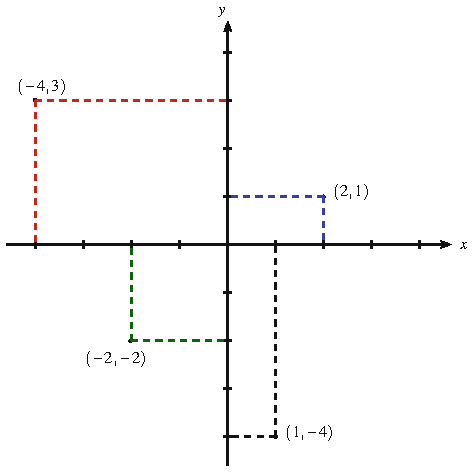
\includegraphics[width=0.562\linewidth]{images/vector/fig-2-1.pdf}
  \caption{$\mathbb{R}^2$ 的笛卡尔坐标系, 其中显示了点 $(2,1)$、$(-4,3)$、$(-2,-2)$ 与 $(1,-4)$.}
  \label{fig:2-1}
\end{figure}

\begin{figure}[htbp]
  \centering
  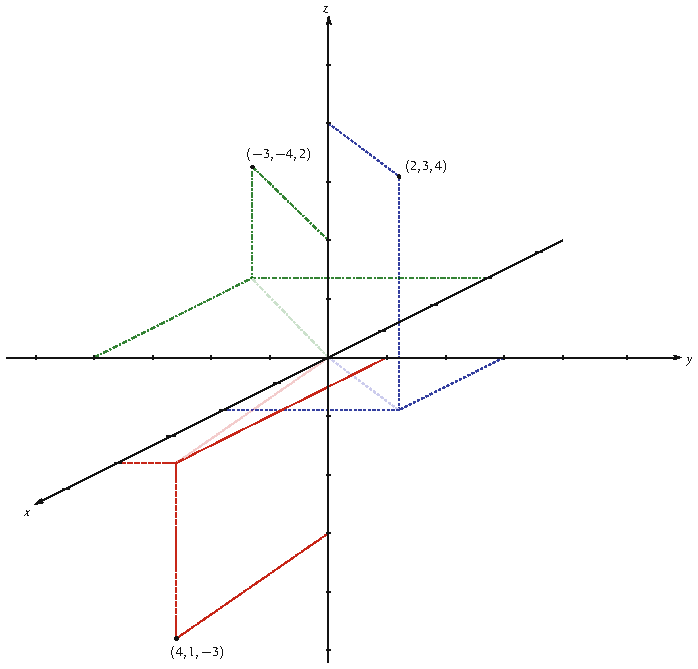
\includegraphics[width=0.932\linewidth]{images/vector/fig-2-2.pdf}
  \caption{$\mathbb{R}^3$ 的笛卡尔坐标系, 其中显示了点 $(2,3,4)$、$(-3,-4,2)$ 与 $(4,1,-3)$}
  \label{fig:2-2}
\end{figure}

注意 $\mathbb{R}^n$ 中点的记号与 $\mathbb{R}^n$ 中向量的记号之间的差别. 例如, $\mathbb{R}^2$ 或 $\mathbb{R}^3$ 中的点记为 $p=(x,y)$ 或 $p=(x,y,z)$, 其中 $x,y,z\in\mathbb{R}$；而 $\mathbb{R}^2$ 或 $\mathbb{R}^3$ 中的向量记为
\[
v=\binom{x}{y}\qquad\text{或}\qquad v=\begin{bmatrix}x\\y\\z\end{bmatrix},
\]
其中 $x,y,z\in\mathbb{R}$. 任意 $n$ 的 $\mathbb{R}^n$ 中的点与向量也类似地表示. 这里有一个微妙的区别, 在微积分课程中几乎总是被一带而过, 尤其是在多元微积分或向量微积分中, 然而这是一个非常重要的区别.
\begin{itemize}
  \item 我们把点的集合 $p=(x_1,x_2,\ldots,x_n)$（其中 $x_1,x_2,\ldots,x_n\in\mathbb{R}$）称为流形 $\mathbb{R}^n$.
  \item 我们把向量的集合 $v=\begin{bmatrix}x_1\\x_2\\\vdots\\x_n\end{bmatrix}$（其中 $x_1,x_2,\ldots,x_n\in\mathbb{R}$）称为向量空间 $\mathbb{R}^n$.
\end{itemize}

这一区别在微积分课程中被一带而过的原因之一是, 大多数微积分学生尚未修过线性代数课程, 还不知道什么是向量空间. 此外, 通过一点数学上模糊而不精确的处理, 确实可以不甚了解向量空间的技术定义就``做''向量微积分. 流形 $\mathbb{R}^2$ 和向量空间 $\mathbb{R}^2$ 看起来完全一样, 却是完全不同的空间. 它们已在图 \ref{fig:2-3} 中画出. 流形 $\mathbb{R}^2$ 包含点, 向量空间 $\mathbb{R}^2$ 包含向量. 当然, 就 $\mathbb{R}^2$、$\mathbb{R}^3$ 甚至 $\mathbb{R}^n$ 而言, 这些空间可以自然地等同. 也就是说, 它们实际上是相同的. 那么为什么做出这一区别如此重要呢？做出这一区别之所以重要有几个原因. 第一, 清楚地区分我们的空间将帮助我们更好地理解微分形式理论；第二, 当我们最终到达更一般的流形时, 大多数流形并不具有向量空间结构, 所以我们不想养成把流形也当作向量空间的坏习惯.

\begin{figure}[htbp]
  \centering
  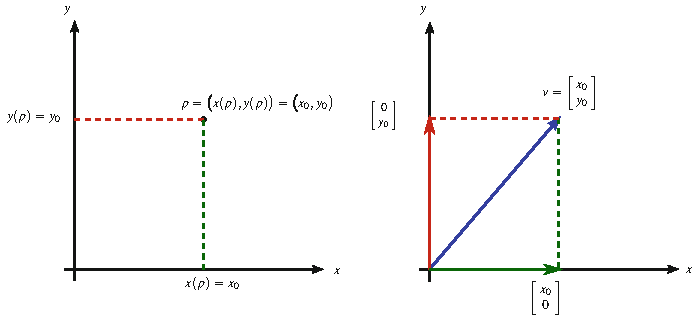
\includegraphics[width=0.938\linewidth]{images/vector/fig-2-3.pdf}
  \caption{流形 $\mathbb{R}^2$（左）与向量空间 $\mathbb{R}^2$（右）}
  \label{fig:2-3}
\end{figure}

现在让我们花一点时间回顾 $\mathbb{R}^2$ 和 $\mathbb{R}^3$ 上老式的普通函数. 我们将考虑实值函数, 它仅仅意味着值域（或陪域）是实数集 $\mathbb{R}$ 或实数集的某个子集. 来自 $\mathbb{R}^2$ 的实值函数最容易可视化, 因为它们可以在三维空间中作图. 考虑由 $f(x,y)=x^3+y^2-3xy$ 定义的实值函数 $f:\mathbb{R}^2\to\mathbb{R}$. 例如, $f(2,3)=(2)^3+(3)^2-3(2)(3)=-1$, $f(5,-2)=(5)^3+(-2)^2-3(5)(-2)=159$, $f(-3,-1)=(-3)^3+(-1)^2-3(-3)(-1)=-35$. 从 $\mathbb{R}^2$ 到 $\mathbb{R}$ 的函数通过点集 $(x,y,f(x,y))$ 在 $\mathbb{R}^3$ 中作图. 函数 $f(x,y)=x^3+y^2-3xy$ 如图 \ref{fig:2-4} 所示. 有时我们写 $f(p)$, 其中 $p=(x,y)$. 通过这样做, 我们强调输入 $(x,y)$ 是定义域中的一个点.

\begin{figure}[htbp]
  \centering
  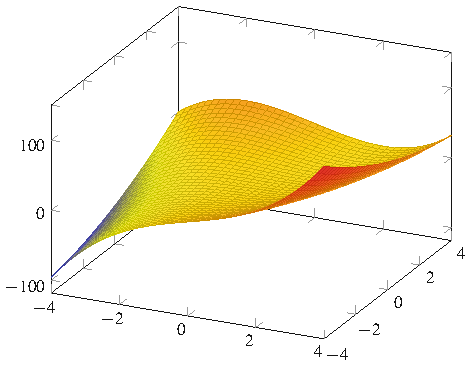
\includegraphics[width=0.559\linewidth]{images/vector/fig-2-4.pdf}
  \caption{函数 $f(x,y)=x^3+y^2-3xy$ 的图像}
  \label{fig:2-4}
\end{figure}

作为进一步的说明, 函数 $f(x,y)=xy$ 和 $f(x,y)=x^2+y^2$ 的图像如图 \ref{fig:2-5} 所示. 和之前一样, 实际作图所用的点集是 $\mathbb{R}^3$ 中的点 $(x,y,f(x,y))$, 因此可以看出, 画函数 $f:\mathbb{R}^2\to\mathbb{R}$ 的图像需要三个维度. 这意味着我们不能准确地画出任何函数 $f:\mathbb{R}^n\to\mathbb{R}$（$n\geq3$）的图像. 然而, 当我们想尝试可视化或描绘 $n\geq3$ 的函数 $f:\mathbb{R}^n\to\mathbb{R}$ 时, 我们常常继续画与图 \ref{fig:2-4} 和 \ref{fig:2-5} 类似的不准确的漫画.

\begin{figure}[htbp]
  \centering
  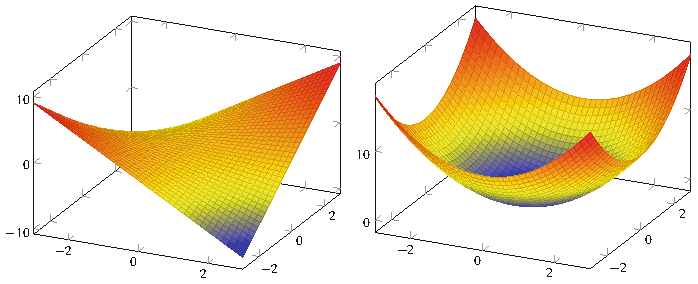
\includegraphics[width=0.960\linewidth]{images/vector/fig-2-5.pdf}
  \caption{作为二元函数图像示例的函数 $f(x,y)=xy$（左）与 $f(x,y)=x^2+y^2$（右）在 $\mathbb{R}^3$ 中的图像}
  \label{fig:2-5}
\end{figure}

我们将对流形 $\mathbb{R}^n$ 上的``函数''和向量空间 $\mathbb{R}^n$ 上的``函数''使用不同的名称. 流形 $\mathbb{R}^n$ 上的函数就简称为函数, 或者有时, 如果我们想强调值域是实数集, 就称为实值函数. 然而, 当值域是实数集时, 向量空间 $\mathbb{R}^n$ 上的``函数''称为泛函；当值域是另一个向量空间时, 称为变换. 我们已经花了一些时间考虑某一类泛函, 即满足
\[
f(v+w)=f(v)+f(w),\qquad f(cv)=cf(v)
\]
的线性泛函, 其中 $v$ 和 $w$ 是向量, $c$ 是实数. 所以, 流形 $\mathbb{R}^n$ 与向量空间 $\mathbb{R}^n$ 的区别隐含在我们的用语中：
\[
\text{函数 }f:\text{（流形）}\mathbb{R}^n\to\mathbb{R},\qquad
\text{泛函 }f:\text{（向量空间）}\mathbb{R}^n\to\mathbb{R}.
\]

现在, 我们将考虑一个从 $\mathbb{R}^n$ 到 $\mathbb{R}$ 的非常特殊的函数. 我们先用 $\mathbb{R}^2$ 作为例子. 我们要看的特殊函数称为坐标函数. 目前我们只看笛卡尔坐标函数.

考虑流形 $\mathbb{R}^2$ 中由笛卡尔坐标 $(3,5)$ 给出的点 $p$. 那么坐标函数
\[
x:\mathbb{R}^2\to\mathbb{R},\qquad p\longmapsto x(p)
\]
挑出第一个坐标, 即 $x(p)=x(3,5)=3$；坐标函数
\[
y:\mathbb{R}^2\to\mathbb{R},\qquad p\longmapsto y(p)
\]
挑出第二个坐标, $y(p)=y(3,5)=5$. 这在图 \ref{fig:2-6} 中作了说明.

\begin{figure}[htbp]
  \centering
  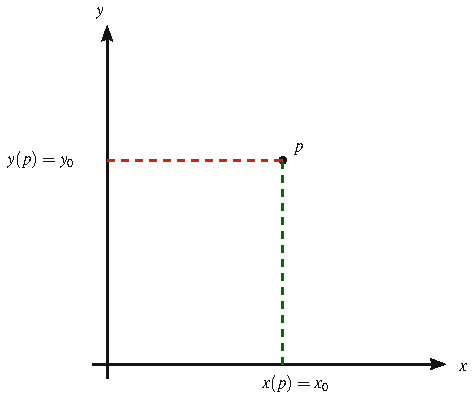
\includegraphics[width=0.562\linewidth]{images/vector/fig-2-6.pdf}
  \caption{坐标函数 $x:\mathbb{R}^2\to\mathbb{R}$ 与 $y:\mathbb{R}^2\to\mathbb{R}$ 分别挑出点 $p\in\mathbb{R}^2$ 的坐标值 $x_0$ 与 $y_0$}
  \label{fig:2-6}
\end{figure}

事实上, 尽管你习惯于把 $(3,5)$ 想成一个点, 但一个点实际上比这更抽象. 一个点独立于其坐标而存在. 例如, 你有时会看到这样的写法：
\[
p=\bigl(x(p),y(p)\bigr),
\]
例如, 对于我们上面给出的那个点, 有 $x(p)=3$, $y(p)=5$.

这里有一些我们需要习惯的歧义. 通常 $x$ 和 $y$ 被用来表示坐标函数 $x$ 和 $y$ 的输出值. 所以, 我们可能会遇到像下面这样有歧义的陈述
\[
x(p)=x,\qquad y(p)=y,
\]
其中等式左边的 $x$ 和 $y$ 是从 $\mathbb{R}^2$ 到 $\mathbb{R}$ 的坐标函数, 而右边的 $x$ 和 $y$ 是实数, 即 $\mathbb{R}$ 的元素. 学会识别 $x$ 和 $y$ 何时是坐标函数、何时是实数值, 需要一点练习, 你必须仔细观察它们是如何被使用的. 这种区别有时会被指出, 但常常被一带而过.

即使点是抽象的、独立于坐标的, 我们实际上也不能不给出一个``地址''就谈论一个特定的点. 这实际上正是坐标函数所做的, 它们被用来给点一个``地址''.

$\mathbb{R}^3$ 上（就此而言还有 $\mathbb{R}^n$ 上）的坐标函数是完全类似的. 例如, 在 $\mathbb{R}^3$ 上有三个坐标函数
\begin{align*}
x:\mathbb{R}^3\to\mathbb{R},\qquad y:\mathbb{R}^3\to\mathbb{R},\qquad z:\mathbb{R}^3\to\mathbb{R}, \\
p\longmapsto x(p),\qquad p\longmapsto y(p),\qquad p\longmapsto z(p),
\end{align*}
它们挑出点 $p$ 的 $x$、$y$、$z$ 坐标, 如图 \ref{fig:2-7} 所示.

\begin{figure}[htbp]
  \centering
  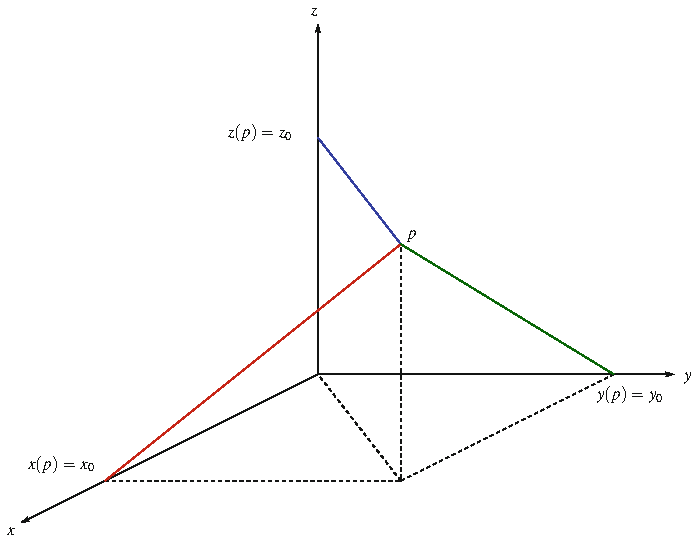
\includegraphics[width=0.827\linewidth]{images/vector/fig-2-7.pdf}
  \caption{坐标函数 $x:\mathbb{R}^3\to\mathbb{R}$、$y:\mathbb{R}^3\to\mathbb{R}$、$z:\mathbb{R}^3\to\mathbb{R}$ 分别挑出点 $p\in\mathbb{R}^3$ 的坐标值 $x_0,y_0,z_0$}
  \label{fig:2-7}
\end{figure}

当然, 笛卡尔坐标函数并不是仅有的坐标函数. 极坐标、球坐标和柱坐标函数是你可能遇到过的其他例子. 我们将在后面更详细地讨论这些坐标系, 但目前我们只考虑一个例子. 考虑点 $p=\bigl(x(p),y(p)\bigr)=(3,5)$. 极坐标 $r$ 和 $\theta$ 通常由 $x=r\cos(\theta)$ 和 $y=r\sin(\theta)$ 给出. 假设我们想求点 $p$ 用极坐标表示的``地址''. 也就是说, 我们想求 $p=\bigl(r(p),\theta(p)\bigr)$.
由于我们已知用 $x$ 和 $y$ 坐标表示的 $p$, 我们可以写 $r=\sqrt{x^2+y^2}$ 和 $\theta=\arctan\frac{y}{x}$. 于是我们有
\begin{align*}
p=\bigl(r(p),\theta(p)\bigr)
&=\Bigl(r\bigl(x(p),y(p)\bigr),\theta\bigl(x(p),y(p)\bigr)\Bigr)\\
&=\left(\sqrt{x(p)^2+y(p)^2},\;\arctan\frac{y(p)}{x(p)}\right)\\
&=\left(\sqrt{3^2+5^2},\;\arctan\frac{5}{3}\right)\\
&=\left(\underbrace{\sqrt{34}}_{r},\;\underbrace{\arctan\frac{5}{3}}_{\theta}\right)\\
&\approx(5.831,\;59.036).
\end{align*}
这里同样的歧义也适用, $r$ 和 $\theta$ 既可以是坐标函数, 也可以是坐标函数给出的值.

\section{切空间与向量场}

让我们回顾一下目前所做的工作. 我们已经回顾了向量空间, 并把 $\mathbb{R}^n$ 作为向量空间讨论, 即作为形如
\[
v=\begin{bmatrix}x_1\\\vdots\\x_n\end{bmatrix}
\]
（其中 $x_1,\ldots,x_n\in\mathbb{R}$）的向量的集合来讨论. 然后我们又把 $\mathbb{R}^n$ 作为流形讨论, 即作为点 $(x_1,\ldots,x_n)$（其中 $x_1,\ldots,x_n\in\mathbb{R}$）的集合来讨论. 我们还回顾了向量空间 $\mathbb{R}^n$ 上的线性泛函和流形 $\mathbb{R}^n$ 上的函数, 并引入了坐标函数. 现在我们来看看流形 $\mathbb{R}^n$ 如何与向量空间 $\mathbb{R}^n$ 相联系. 我们这样做的动机是做微积分的愿望. 嗯, 至少目前是为了取方向导数.

然而, 为了帮助我们更好地想象正在发生的事情, 我们将先考虑三个流形：$S^1$、$S^2$ 和 $T$. 流形 $S^1$ 就是一个圆, 流形 $S^2$ 是球面, 流形 $T$ 是环面, 看起来像一个甜甜圈. 目前我们将相当不精确. 我们希望你带走对流形是什么的一般感受, 而不是用技术细节压垮你. 目前我们只说流形是一个局部为欧几里得的空间. 我们的意思是, 如果我们观察流形的非常小的一部分, 那部分看起来就像某个自然数 $n$ 的 $\mathbb{R}^n$.

我们将对我们选择考察的三个流形说明这个思想. 圆 $S^1$ 局部像 $\mathbb{R}^1$, 这解释了 $S$ 上的上标 1. 在图 \ref{fig:2-8} 中, 我们几次放大 1-球面 $S^1$ 的一小部分, 以看出局部地流形 $S^1$ 看起来像 $\mathbb{R}^1$. 类似地, 在图 \ref{fig:2-9} 中我们放大 2-球面 $S^2$ 的一小部分, 以看出它局部像 $\mathbb{R}^2$；在图 \ref{fig:2-10} 中我们放大环面 $T$ 的一小部分, 以看出它局部也像 $\mathbb{R}^2$.

\begin{figure}[htbp]
  \centering
  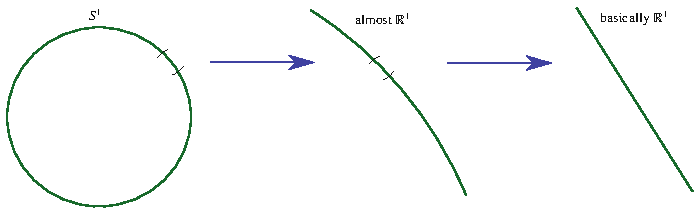
\includegraphics[width=0.944\linewidth]{images/vector/fig-2-8.pdf}
  \caption{这里放大了 1-球面（即圆）$S^1$ 的一小部分, 以显示局部地流形 $S^1$ 看起来像 $\mathbb{R}^1$}
  \label{fig:2-8}
\end{figure}

\begin{figure}[htbp]
  \centering
  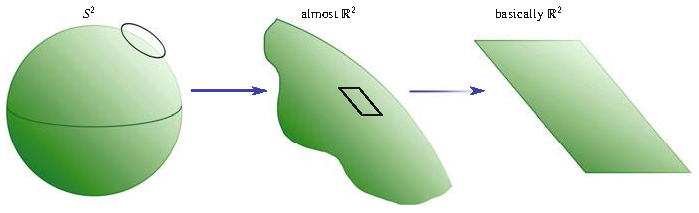
\includegraphics[width=0.953\linewidth]{images/vector/fig-2-9.pdf}
  \caption{这里放大了 2-球面 $S^2$ 的一小部分, 以显示局部地流形 $S^2$ 看起来像 $\mathbb{R}^2$}
  \label{fig:2-9}
\end{figure}

\begin{figure}[htbp]
  \centering
  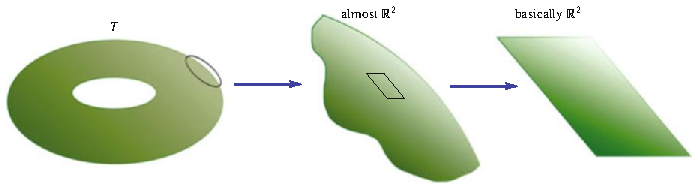
\includegraphics[width=0.960\linewidth]{images/vector/fig-2-10.pdf}
  \caption{这里放大了环面 $T$ 的一小部分, 以显示局部地流形 $T$ 看起来像 $\mathbb{R}^2$}
  \label{fig:2-10}
\end{figure}

这些例子的要点是, 即使这些示例流形局部看起来像 $\mathbb{R}^1$ 和 $\mathbb{R}^2$, 全局它们却并非如此. 也就是说, 它们的全局行为更为复杂；这些空间以欧几里得空间所没有的方式扭曲并重新连接自身.

现在我们引入切空间的概念. 同样, 我们想给你关于切空间是什么的一般感受, 而不是用技术细节压垮你, 这些将在 10.2 节给出. 从微积分中你应该记得曲线在其上某点处的切线是什么. 曲线的每个点都有它自己的切线, 如图 \ref{fig:2-11} 所示. 可以看出, 一维曲线的切空间是直线, 也就是说, 它们也是一维的.

类似地, 二维曲面在其每个点处都有一个切平面, 如图 \ref{fig:2-12} 所示. 流形在点 $p$ 处的切空间基本上是经过流形上点 $p$ 的光滑曲线在 $p$ 处的所有切线的集合. 这在图 \ref{fig:2-13} 中作了说明, 我们在那里画了一个点 $p$、五条经过它的光滑曲线, 以及这些曲线在点 $p$ 处的五条切线. 在这两幅图中切空间都是一个平面.

\begin{figure}[htbp]
  \centering
  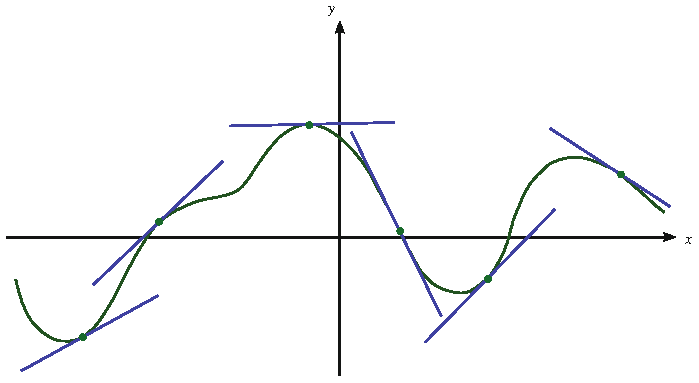
\includegraphics[width=0.838\linewidth]{images/vector/fig-2-11.pdf}
  \caption{这里画出一条曲线, 并在几个点处画出切线}
  \label{fig:2-11}
\end{figure}

\begin{figure}[htbp]
  \centering
  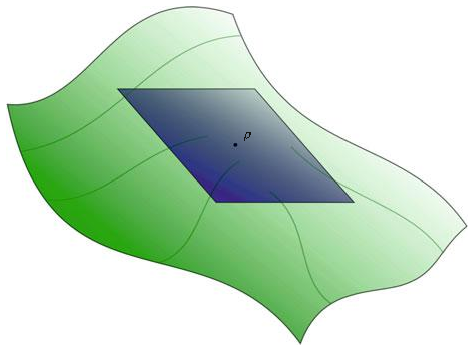
\includegraphics[width=0.610\linewidth]{images/vector/fig-2-12.pdf}
  \caption{这里画出一个二维曲面以及在一个点处画出的切平面}
  \label{fig:2-12}
\end{figure}

\begin{figure}[htbp]
  \centering
  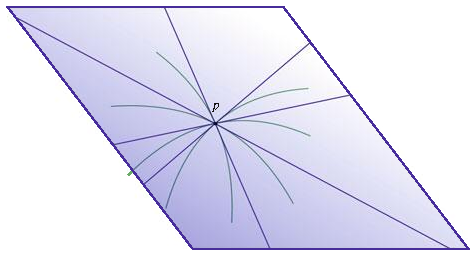
\includegraphics[width=0.662\linewidth]{images/vector/fig-2-13.pdf}
  \caption{二维曲面在点 $p$ 处的切平面是曲面上经过 $p$ 的曲线在 $p$ 处所有切线的集合}
  \label{fig:2-13}
\end{figure}

如果你想象三维流形中的一个点以及所有可能经过该点的曲线, 然后想象这些曲线在该点处的所有切线, 你就会看到该点处的切空间是三维的. 事实证明, 在``好''点处的切空间与该点处流形的维数相同. 在本书中我们不讨论在这个意义上不``好''的点处的流形. 事实上, 切空间无非就是正确 $n$ 值的向量空间 $\mathbb{R}^n$. 因为切空间是向量空间, 我们把点 $p$ 处的切空间想成点 $p$ 处所有切向量的集合. 我们使用切空间的特殊记号. $T_pM$ 或 $T_p(M)$ 表示流形 $M$ 在点 $p$ 处的切空间.

\begin{figure}[htbp]
  \centering
  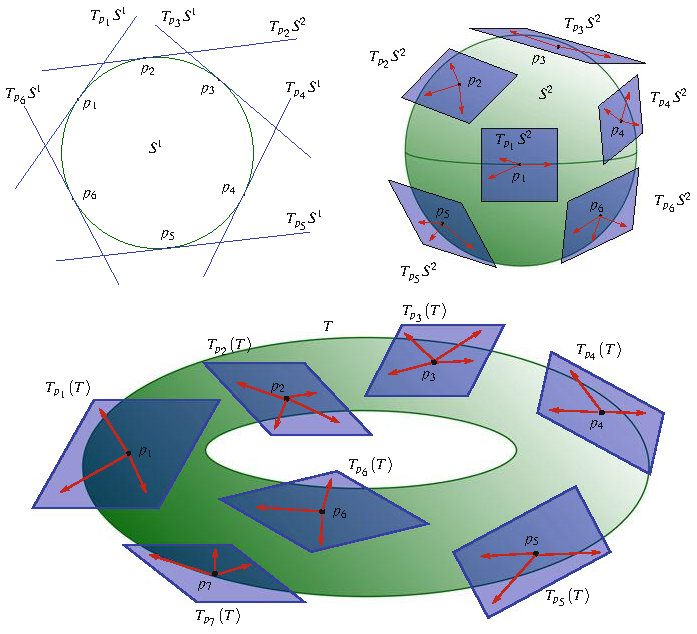
\includegraphics[width=0.826\linewidth]{images/vector/fig-2-14.pdf}
  \caption{流形 $S^1$ 以及若干画出的切线（左上）. 流形 $S^2$ 以及若干画出的切平面（右上）. 流形 $T$ 以及若干画出的切平面（下）. 对流形 $S^2$ 和 $T$, 还画出了每个切平面中的若干向量}
  \label{fig:2-14}
\end{figure}

为了更好了解流形的切空间集合长什么样, 我们在图 \ref{fig:2-14} 中为我们之前看过的三个简单流形画出了若干切空间：圆 $S^1$、球面 $S^2$ 和环面 $T$. 对二维切空间我们还画出了切空间的一些元素, 即从点 $p$ 出发的向量. 圆的切空间记为 $T_pS^1$, 球面的切空间记为 $T_pS^2$, 环面的切空间记为 $T_p(T)$. 这里使用圆括号只是因为 $T_pT$ 看起来有点奇怪.

尽管我们对流形 $\mathbb{R}^2$ 和 $\mathbb{R}^3$ 相当熟悉, 但想象这些流形的切空间有点奇怪, 尽管这正是你在向量微积分以来一直在隐式做的事情. 流形 $\mathbb{R}^2$ 在点 $p$ 处的切空间是基点在点 $p$ 的所有向量的集合. 在向量微积分中我们大量处理带不同基点的向量, 但我们总是把这些向量简单地想成在流形 $\mathbb{R}^2$ 或 $\mathbb{R}^3$ 中. 现在我们把这些向量想成属于附着在该点的一个单独的向量空间 $\mathbb{R}^2$ 或 $\mathbb{R}^3$ 的副本, 并称之为切空间.

\begin{figure}[htbp]
  \centering
  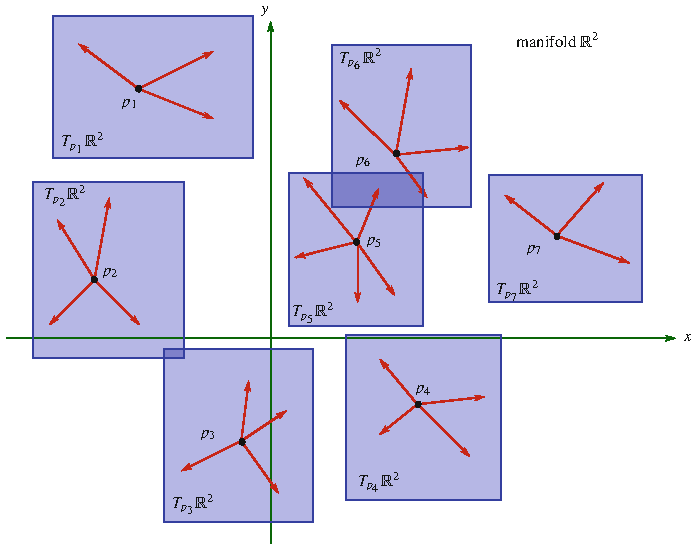
\includegraphics[width=0.960\linewidth]{images/vector/fig-2-15.pdf}
  \caption{流形 $\mathbb{R}^2$ 以及七个不同点处的切空间 $T_{p_i}\mathbb{R}^2$. 每个切空间中画出了若干向量}
  \label{fig:2-15}
\end{figure}

\begin{figure}[htbp]
  \centering
  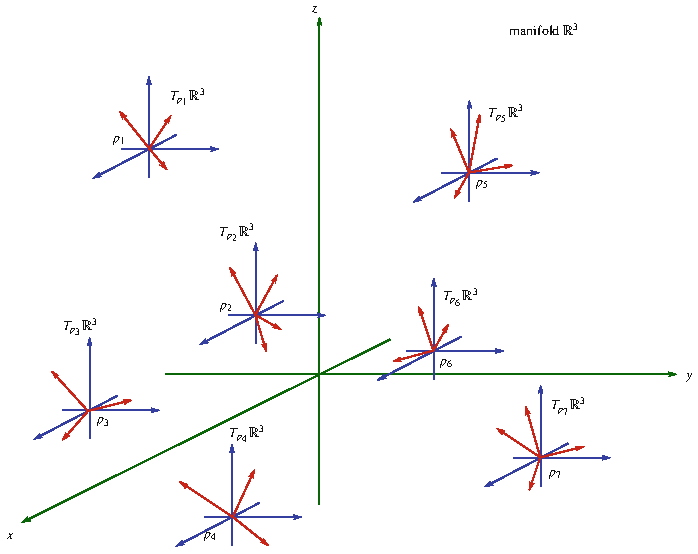
\includegraphics[width=0.960\linewidth]{images/vector/fig-2-16.pdf}
  \caption{流形 $\mathbb{R}^3$ 以及七个不同点处的切空间 $T_{p_i}\mathbb{R}^3$. 每个切空间中画出了若干向量}
  \label{fig:2-16}
\end{figure}

图 \ref{fig:2-15} 试图帮助你想象正在发生的事情. 图中画出了流形 $\mathbb{R}^2$ 以及七个不同点 $p_1,\ldots,p_7$ 处的切空间 $T_{p_i}\mathbb{R}^2$. 每个切空间 $T_p\mathbb{R}^2$ 都同构于（``等同于''）$\mathbb{R}^2$. 虽然我们只画出了七个点处的切空间, 但事实上对每个点 $p\in\mathbb{R}^2$ 都有一个单独的切空间 $T_p\mathbb{R}^2$.

图 \ref{fig:2-16} 试图帮助你想象 $\mathbb{R}^3$ 的切空间. 同样, 图中画出了流形 $\mathbb{R}^3$ 以及七个不同点 $p_1,\ldots,p_7$ 处的切空间 $T_{p_i}\mathbb{R}^3$. 每个切空间 $T_p\mathbb{R}^3$ 都自然同构于 $\mathbb{R}^3$. 同样, 虽然我们只画出了七个点处的切空间, 但事实上对每个点 $p\in\mathbb{R}^3$ 都有一个单独的切空间 $T_p\mathbb{R}^3$.

从现在起, 我们经常把向量的基点包含在记号中. 例如, 向量 $v_p$ 表示基点在流形 $M$ 的点 $p$ 处的向量 $v$. 显然, 向量 $v_p$ 属于（即是其中的元素）切空间 $T_pM$. 所以, 例如, 我们有
\[
\binom{1}{1}_{(-2,-3)}\in T_{(-2,-3)}\mathbb{R}^2,\qquad
\binom{1}{1}_{(-1,4)}\in T_{(-1,4)}\mathbb{R}^2,\qquad
\binom{1}{1}_{(2,4)}\in T_{(2,4)}\mathbb{R}^2,
\]
以及
\[
\begin{bmatrix}1\\1\\1\end{bmatrix}_{(-2,-3,-5)}\in T_{(-2,-3,-5)}\mathbb{R}^3,\qquad
\begin{bmatrix}1\\1\\1\end{bmatrix}_{(-1,4,3)}\in T_{(-1,4,3)}\mathbb{R}^3,\qquad
\begin{bmatrix}1\\1\\1\end{bmatrix}_{(2,4,-1)}\in T_{(2,4,-1)}\mathbb{R}^3.
\]

流形 $M$ 连同附着在流形每个点处的向量空间 $T_pM$ 的一个副本, 称为流形 $M$ 的切丛, 记为 $TM$ 或 $T(M)$. 流形 $M$ 的切丛的漫画版常常画成图 \ref{fig:2-17} 那样, 对流形和切空间都使用一维表示.

\begin{figure}[htbp]
  \centering
  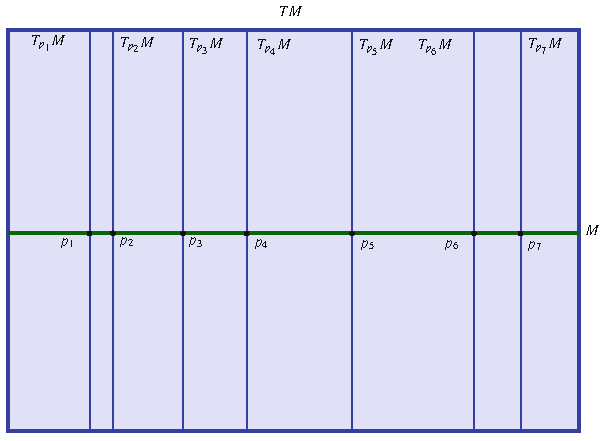
\includegraphics[width=0.749\linewidth]{images/vector/fig-2-17.pdf}
  \caption{流形 $M$ 上切丛 $TM$ 的漫画. 显示了七个切空间 $T_{p_i}M$}
  \label{fig:2-17}
\end{figure}

若 $M$ 是 $n$ 维流形, 则 $TM$ 是 $2n$ 维的. 这在直观上是合理的, 因为要精确指定 $TM$ 中任意元素（向量）, 你需要指定向量部分（需要 $n$ 个数）和基点（也需要 $n$ 个数）. 因此, $T\mathbb{R}^2$ 有四个维度, $T\mathbb{R}^3$ 有六个维度. 事实上, 流形 $M$ 的切丛 $TM$ 本身也是一个流形. 因此, 若 $M$ 是 $n$ 维流形, 则 $TM$ 是 $2n$ 维流形.

现在我们将非常简要地引入向量场的概念. 毫无疑问, 你在向量微积分中已经接触过向量场的思想, 在那里它通常定义在 $\mathbb{R}^2$ 或 $\mathbb{R}^3$ 上, 是一个给每个点 $(x,y)\in\mathbb{R}^2$ 或 $(x,y,z)\in\mathbb{R}^3$ 指派一个向量
\[
\binom{v_1}{v_2}_{(x,y)}\qquad\text{或}\qquad
\begin{bmatrix}v_1\\v_2\\v_3\end{bmatrix}_{(x,y,z)}
\]
的向量值函数. $\mathbb{R}^2$ 上的一个向量场示例如图 \ref{fig:2-18} 所示.

\begin{figure}[htbp]
  \centering
  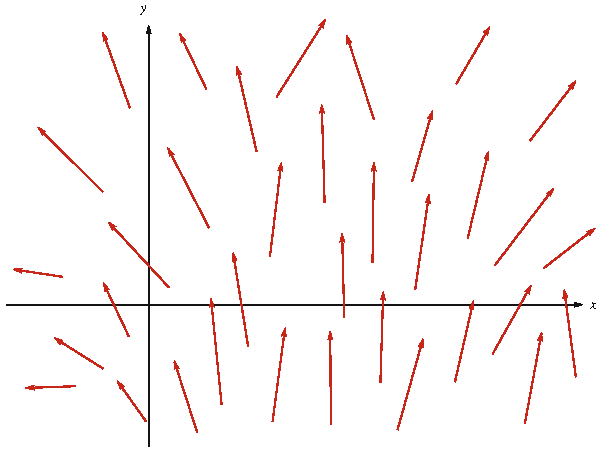
\includegraphics[width=0.756\linewidth]{images/vector/fig-2-18.pdf}
  \caption{画在流形 $\mathbb{R}^2$ 上的向量场. 回想一下, 所示的每个向量都是切空间的元素, 并不真正在流形 $\mathbb{R}^2$ 中}
  \label{fig:2-18}
\end{figure}

若可以在流形上找到一些曲线, 使得向量场中的所有向量都与这些曲线相切, 则称向量场是光滑的. 这些曲线称为向量场的积分曲线, 而求这些曲线本质上就是微分方程的全部内容. 图 \ref{fig:2-19} 显示了 $\mathbb{R}^2$ 上一个光滑向量场的若干积分曲线.

\begin{figure}[htbp]
  \centering
  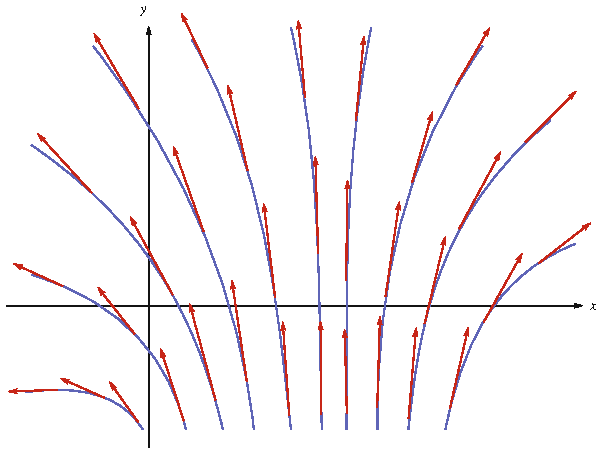
\includegraphics[width=0.756\linewidth]{images/vector/fig-2-19.pdf}
  \caption{画在流形 $\mathbb{R}^2$ 上的光滑向量场. 同样, 回想一下, 所示的每个向量都是切空间的元素, 并不真正在流形 $\mathbb{R}^2$ 中}
  \label{fig:2-19}
\end{figure}

虽然我们当然不打算在这里深入微分方程, 但我们想做的是引入一种思考向量场的新方式. 注意, 流形（如 $\mathbb{R}^2$ 或 $\mathbb{R}^3$）上的向量场在流形的每个点处给我们一个向量. 但流形 $M$ 的点 $p$ 处的向量 $v_p$ 是该点切空间 $T_pM$ 的元素. 所以, 给一个向量场与给 $M$ 的每个切空间的一个元素是同一回事. 这常被称为切丛 $TM$ 的一个截面. 在图形上, 我们常常像图 \ref{fig:2-20} 那样可视化切丛的截面.

\begin{figure}[htbp]
  \centering
  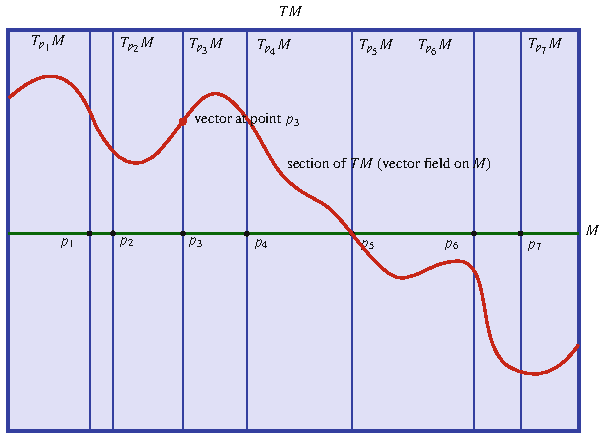
\includegraphics[width=0.749\linewidth]{images/vector/fig-2-20.pdf}
  \caption{流形 $M$ 上切丛的一个截面的漫画. $TM$ 的截面就是 $M$ 上的向量场. 向量场在 $M$ 的点 $p_3$ 处的向量被画成截面中 $T_{p_3}M$ 里的那个点. 注意, 在这种漫画表示中, 点 $p_5$ 处的向量将是零向量}
  \label{fig:2-20}
\end{figure}

\begin{question}\label{q:2-1}
在进入下一节之前, 让我们花一点时间回顾导数是怎么回事. 考虑由 $f(x)=\frac{x^2}{2}+2$ 给出的函数 $f:\mathbb{R}\to\mathbb{R}$.
\begin{enumerate}
  \item[(a)] 画出函数 $f(x)=\frac{x^2}{2}+2$ 的图像.
  \item[(b)] 求 $f(x)$ 的导数.
  \item[(c)] $f(2)$ 是什么？$f(3)$ 是什么？在点 $\bigl(2,f(2)\bigr)$ 和 $\bigl(3,f(3)\bigr)$ 之间画一条直线.
  \item[(d)] 这条割线的斜率是多少？
  \item[(e)] 写出差商定义导数的极限.
  \item[(f)] 用这个定义求 $f$ 在 $x=2$ 处的导数. 它与你上面得到的答案一致吗？
  \item[(g)] $f$ 在 $x=2$ 处的导数是一个数. 解释这个数代表什么.
\end{enumerate}
通过上面的问题, 你现在应该记得导数基本上就是函数图像在某点处切线的斜率.
\end{question}

\section{方向导数}

现在是时候探讨我们为什么要用这些材料了. 假设我们在流形 $\mathbb{R}^n$ 上有一个实值函数 $f$, 即 $f:\mathbb{R}^n\to\mathbb{R}$. 我们如何使用流形上某个给定点 $p$ 处的向量 $v_p$ 呢？一个自然的做法是取 $f$ 在点 $p$ 处沿 $v_p$ 方向的方向导数. 考虑图 \ref{fig:2-21}, 其中显示了实值函数 $f:\mathbb{R}\to\mathbb{R}$. 给定定义域中的一个点 $p$, 有两个可能移动的方向, 左或右. 类似地, 如果你有一个基点在该点的向量, 它既可以指向左（像 $v_p$ 那样）, 也可以指向右（像 $w_p$ 那样）. 我们可以问函数在这两个方向中的任一方向上如何变化. 在图 \ref{fig:2-22} 中描绘了实值函数 $f:\mathbb{R}^2\to\mathbb{R}$. 给定定义域中的一个点 $p=(x,y)$, 人们可以在二维中以任意方向移动, 而基点在该点的向量也可以在二维中指向任意方向. 类似地, 我们可以问函数在这些方向中的任意一个方向上如何变化. 在图 \ref{fig:2-23} 中我们选择了其中一个方向, 即由向量
\[
v_p=\binom{a}{b}_{(x,y)}
\]
给出的方向. 我们能利用这个向量求 $f$ 在点 $p$ 处沿 $v_p$ 方向的方向导数. 换句话说, 我们能求出 $f$ 在点 $p$ 处沿 $v_p$ 方向是如何变化的.

\begin{figure}[htbp]
  \centering
  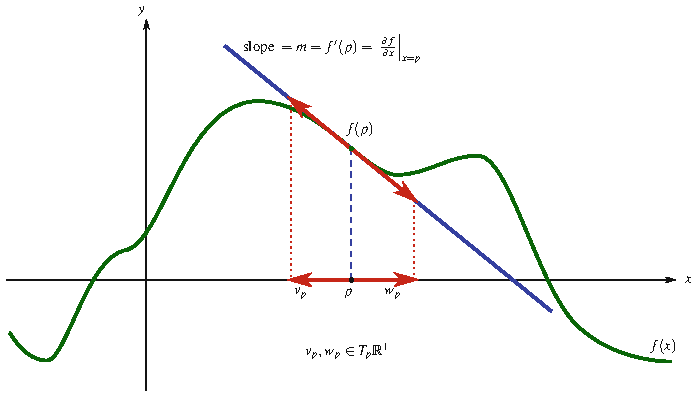
\includegraphics[width=0.877\linewidth]{images/vector/fig-2-21.pdf}
  \caption{从 $p\in\mathbb{R}$ 出发可以在任意一维方向上移动. 换句话说, 可以向右或向左}
  \label{fig:2-21}
\end{figure}

\begin{figure}[htbp]
  \centering
  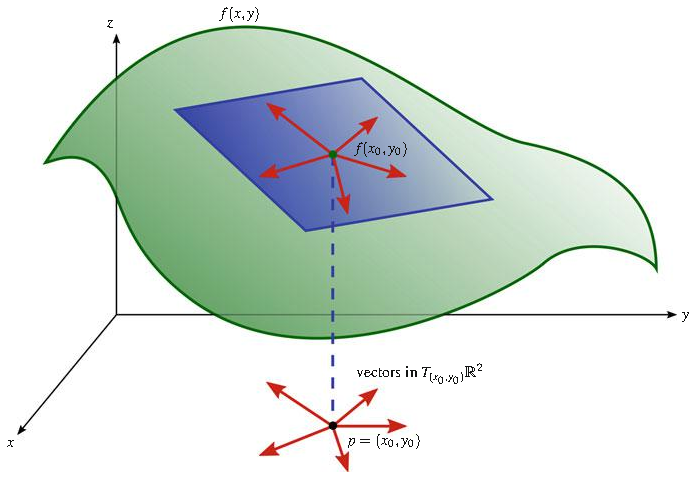
\includegraphics[width=0.829\linewidth]{images/vector/fig-2-22.pdf}
  \caption{从 $p=(x,y)\in\mathbb{R}^2$ 出发可以在二维中以任意方向移动. 图中画出了若干不同的方向}
  \label{fig:2-22}
\end{figure}

\begin{figure}[htbp]
  \centering
  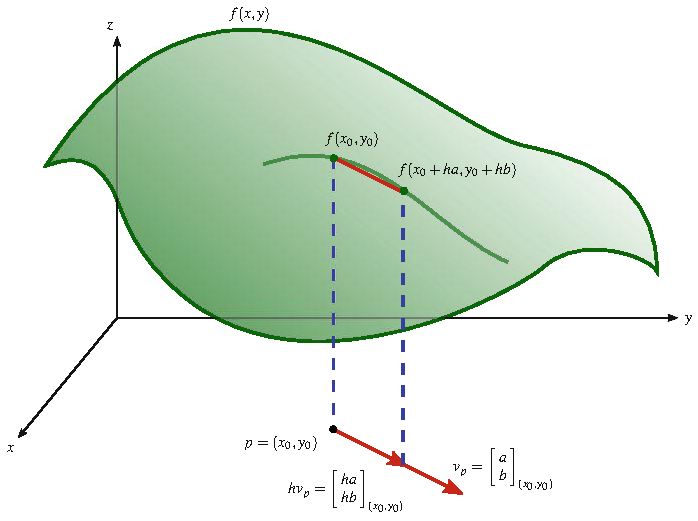
\includegraphics[width=0.834\linewidth]{images/vector/fig-2-23.pdf}
  \caption{求函数 $f:\mathbb{R}^2\to\mathbb{R}$ 的方向导数需要一个某个方向的单位向量以及 $f(x_0+ta,y_0+tb)$ 与 $f(x_0,y_0)$ 的相应值, 它们是差商所必需的}
  \label{fig:2-23}
\end{figure}

注意, 目前我们回到向量微积分的思考方式, 把向量 $v_p$ 想成位于流形 $\mathbb{R}^2$ 中的点 $p$ 处, 而不是在切空间 $T_p\mathbb{R}^2$ 中. 尽管我们刚刚大谈特谈向量不在流形中而在切空间中, 但由于在本节和下一节我们要从向量微积分的观点回顾方向导数的思想, 我们将回到把向量想成位于流形中、基点在某一点. 这样我们就能使用向量微积分的记号, 把注意力集中在相关的思想上, 而不被记号的细微差别拖累.

我们首先考虑方向导数在大多数多元微积分课程中通常是如何引入的. 我们这样做的原因是, 我们想使用的方向导数定义将与大多数向量微积分课程中使用的略有不同, 我们不希望有任何混淆. 你可能见过的定义是这样的.

\begin{definition}[方向导数（单位向量）]\label{def:2-3-1}
函数 $f:\mathbb{R}^2\to\mathbb{R}$ 在 $(x_0,y_0)$ 处沿单位向量 $u=\binom{a}{b}$ 方向的方向导数为
\[
D_uf(x_0,y_0)=\lim_{t\to0}\frac{f(x_0+ta,y_0+tb)-f(x_0,y_0)}{t},
\]
如果这个极限存在.
\end{definition}

\begin{definition}[方向导数（$\mathbb{R}^3$ 情形）]\label{def:2-3-2}
函数 $f:\mathbb{R}^3\to\mathbb{R}$ 在 $(x_0,y_0,z_0)$ 处沿单位向量 $u=\begin{bmatrix}a\\b\\c\end{bmatrix}$ 方向的方向导数为
\[
D_uf(x_0,y_0,z_0)=\lim_{t\to0}\frac{f(x_0+ta,y_0+tb,z_0+tc)-f(x_0,y_0,z_0)}{t},
\]
如果这个极限存在.
\end{definition}

通常向量微积分教科书会把向量写成行向量, 有时像 $[a,b]$, 有时像 $\langle a,b\rangle$. 我们在本书中绝不这样做. 我们总是把向量写成带方括号的列向量, $v=\binom{a}{b}$. 此外, 我们绝不使用尖括号 $\langle\cdot,\cdot\rangle$ 表示向量或点, 虽然有时会看到. 最后, 注意在两个定义中向量 $u$ 必须是单位向量, 这意味着向量的长度为一个单位. 换句话说, 对第一个定义我们必须有 $\sqrt{a^2+b^2}=1$, 对第二个定义我们必须有 $\sqrt{a^2+b^2+c^2}=1$.

为了提醒我们自己一些其他等价的记号, 注意如果我们令 $p=(x_0,y_0)$, 那么我们也可以写
\[
\lim_{t\to0}\frac{f(x_0+ta,y_0+tb)-f(x_0,y_0)}{t}
=\left.\frac{d}{dt}f(p+tu)\right|_{t=0}
\]
而如果我们令 $p=(x_0,y_0,z_0)$, 那么我们也可以写
\[
\lim_{t\to0}\frac{f(x_0+ta,y_0+tb,z_0+tc)-f(x_0,y_0,z_0)}{t}
=\left.\frac{d}{dt}f(p+tu)\right|_{t=0}.
\]
这意味着我们也可以把上面的定义写成
\[
D_uf(x_0,y_0)=\left.\frac{d}{dt}f(p+tu)\right|_{t=0}
\]
和
\[
D_uf(x_0,y_0,z_0)=\left.\frac{d}{dt}f(p+tu)\right|_{t=0}.
\]

假设我们有一个函数 $f:\mathbb{R}^2\to\mathbb{R}$ 和单位向量
\[
u=\binom{1}{0},\qquad v=\binom{0}{1},
\]
那么很容易看出 $D_uf=\frac{\partial f}{\partial x}$、$D_vf=\frac{\partial f}{\partial y}$. 类似地, 对函数 $g:\mathbb{R}^3\to\mathbb{R}$ 和单位向量
\[
u=\begin{bmatrix}1\\0\\0\end{bmatrix},\qquad v=\begin{bmatrix}0\\1\\0\end{bmatrix},\qquad w=\begin{bmatrix}0\\0\\1\end{bmatrix},
\]
我们得到 $D_ug=\frac{\partial g}{\partial x}$、$D_vg=\frac{\partial g}{\partial y}$、$D_wg=\frac{\partial g}{\partial z}$.

\begin{question}\label{q:2-2}
求 $f(x,y)=x^3-3xy+y^2$ 在 $p=(1,2)$ 处沿 $u=\binom{\cos(\pi/6)}{\sin(\pi/6)}$ 方向的导数.
\end{question}

按照你在多元微积分中可能做过的方式, 在做出上述方向导数定义之后, 推导出以下定理.

\begin{theorem}[方向导数的计算公式]\label{thm:2-1}
若 $f:\mathbb{R}^2\to\mathbb{R}$ 是关于 $x$ 和 $y$ 的可微函数, 则 $f$ 沿任意单位向量 $u=\binom{a}{b}$ 方向具有方向导数, 且
\[
D_uf(x,y)=\frac{\partial f}{\partial x}(x,y)\cdot a+\frac{\partial f}{\partial y}(x,y)\cdot b.
\]
\end{theorem}

\begin{proof}[证明梗概]
首先定义一元函数 $g(h)$ 为 $g(h)=f(x_0+ha,y_0+hb)$, 并用它改写 $D_uf$. 然后用链式法则写出 $g(h)$ 的导数. 最后令 $h=0$ 并合并.
\end{proof}

\begin{theorem}[方向导数的计算公式（$\mathbb{R}^3$ 情形）]\label{thm:2-2}
若 $f:\mathbb{R}^3\to\mathbb{R}$ 是关于 $x,y,z$ 的可微函数, 则 $f$ 沿任意单位向量 $u=\begin{bmatrix}a\\b\\c\end{bmatrix}$ 方向具有方向导数, 且
\[
D_uf(x,y,z)=\frac{\partial f}{\partial x}(x,y,z)\cdot a+\frac{\partial f}{\partial y}(x,y,z)\cdot b+\frac{\partial f}{\partial z}(x,y,z)\cdot c.
\]
\end{theorem}

\begin{question}\label{q:2-3}
令 $p=(2,0,-1)$, $v=\frac{1}{\sqrt{14}}\begin{bmatrix}2\\-1\\3\end{bmatrix}$. 求 $D_{v_p}f$, 其中
\begin{enumerate}
  \item[(a)] $f(x,y,z)=y^2z$
  \item[(b)] $f(x,y,z)=e^x\cos(y)$
  \item[(c)] $f(x,y,z)=x^7$
\end{enumerate}
\end{question}

现在我们想探讨为什么规定
\[
u=\binom{a}{b}\qquad\text{或}\qquad u=\begin{bmatrix}a\\b\\c\end{bmatrix}
\]
是单位向量. 我们首先注意到, 经过原点的平面方程由
\[
z=m_xx+m_yy
\]
给出, 如图 \ref{fig:2-24} 所示. 由此很容易证明, $f$ 图像上经过点 $(x_0,y_0,f(x_0,y_0))$ 的平面方程由
\[
z-f(x_0,y_0)=m_x(x-x_0)+m_y(y-y_0)
\]
给出.

\begin{figure}[htbp]
  \centering
  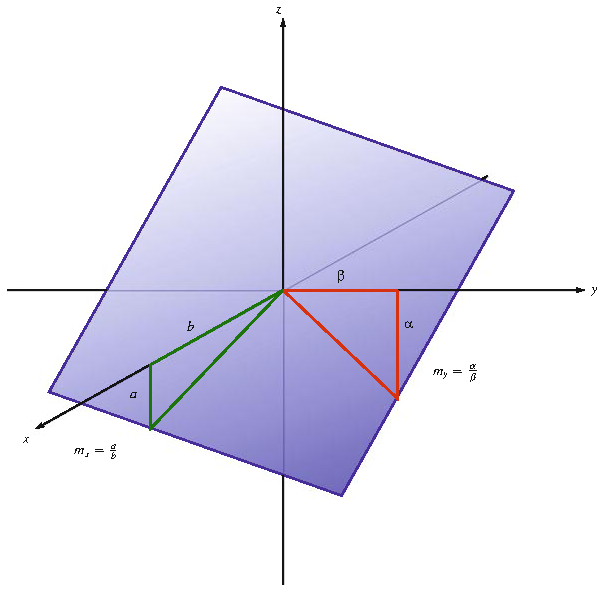
\includegraphics[width=0.777\linewidth]{images/vector/fig-2-24.pdf}
  \caption{经过原点的平面方程由 $z=m_xx+m_yy$ 给出, 其中 $m_x$ 是平面沿 $x$ 轴的斜率, $m_y$ 是平面沿 $y$ 轴的斜率}
  \label{fig:2-24}
\end{figure}

为得到 $f(x,y)$ 在点 $(x_0,y_0,f(x_0,y_0))$ 处切平面 $T(x_0,y_0)$ 的方程, 我们注意到
\begin{align*}
m_x=\frac{\partial f}{\partial x},\qquad m_y=\frac{\partial f}{\partial y} \\
\Rightarrow\quad T(x,y)-f(x_0,y_0)=\left.\frac{\partial f}{\partial x}\right|_{(x_0,y_0)}\cdot(x-x_0)+\left.\frac{\partial f}{\partial y}\right|_{(x_0,y_0)}\cdot(y-y_0), \\
\Rightarrow\quad T(x,y)=f(x_0,y_0)+\left.\frac{\partial f}{\partial x}\right|_{(x_0,y_0)}\cdot(x-x_0)+\left.\frac{\partial f}{\partial y}\right|_{(x_0,y_0)}\cdot(y-y_0),
\end{align*}
如图 \ref{fig:2-25} 所示.

\begin{figure}[htbp]
  \centering
  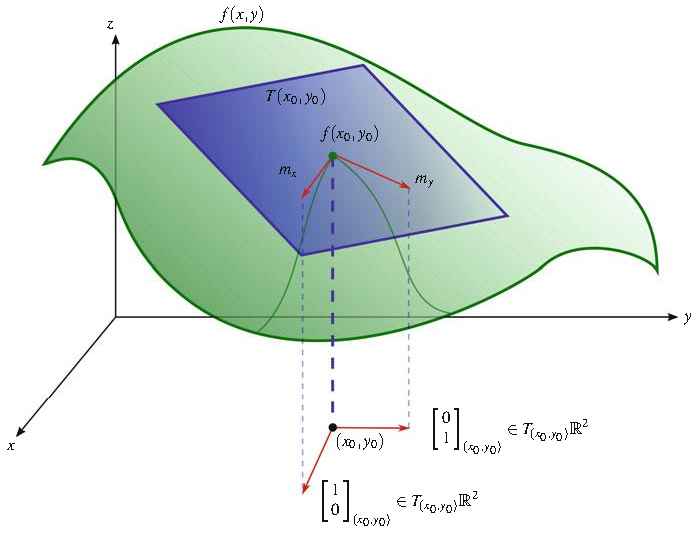
\includegraphics[width=0.891\linewidth]{images/vector/fig-2-25.pdf}
  \caption{$f(x,y)$ 在点 $(x_0,y_0,f(x_0,y_0))$ 处的切平面 $T(x_0,y_0)$}
  \label{fig:2-25}
\end{figure}

考虑点 $(x_0,y_0)$ 处的向量 $u=\binom{a}{b}$, 即 $u=\binom{a}{b}_{(x_0,y_0)}$, 如图 \ref{fig:2-26} 所示. 我们如何求经过点 $f(x_0,y_0)$ 的 $f$ 的图像切线的斜率呢？我们使用 $m=\frac{\text{rise}}{\text{run}}$, 其中显然``run''是向量 $\binom{a}{b}$ 的长度. 我们的 rise, 即高度 $z$ 的变化, 可以用我们上面推导的切平面方程计算, 
\begin{align*}
\frac{\text{rise}}{\text{run}}
&=\frac{T(x_0+a,y_0+b)-T(x_0,y_0)}{\sqrt{a^2+b^2}}\\
&=\frac{\left.\frac{\partial f}{\partial x}\right|_{(x_0,y_0)}\cdot a+\left.\frac{\partial f}{\partial y}\right|_{(x_0,y_0)}\cdot b}{\sqrt{a^2+b^2}}\\
&=\frac{\frac{\partial f}{\partial x}\cdot a+\frac{\partial f}{\partial y}\cdot b}{\sqrt{a^2+b^2}}.
\end{align*}

\begin{figure}[htbp]
  \centering
  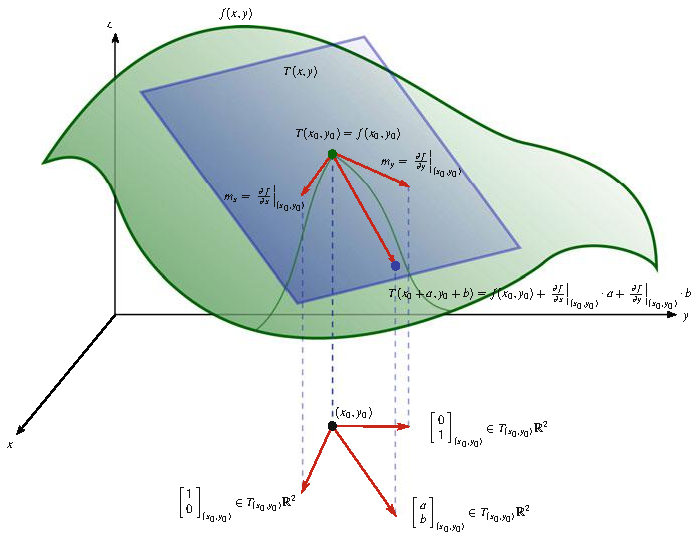
\includegraphics[width=0.960\linewidth]{images/vector/fig-2-26.pdf}
  \caption{$f(x,y)$ 在点 $(x_0,y_0)$ 处的切平面, 其中显示了沿方向 $v=ae_1+be_2$ 的切线}
  \label{fig:2-26}
\end{figure}

注意这与多元微积分中给出的 $D_uf$ 的公式多么接近：
\[
D_uf=\frac{\partial f}{\partial x}\cdot a+\frac{\partial f}{\partial y}\cdot b.
\]
只要向量 $\binom{a}{b}$ 是单位向量, 这两个公式就相同. 因此, 若 $u$ 是单位向量, 则 $D_uf$ 的公式也给出位于切平面内、沿 $\binom{a}{b}$ 方向的切线的斜率. 所以, 通过规定 $u=\binom{a}{b}$ 是单位向量, 我们基本上既保持了导数的定义是切线的斜率, 又保留了一个漂亮的简单导数公式.

我们现在将放宽这一要求, 允许任意向量, 而不只是单位向量. 然而, 我们想保留那个漂亮的公式. 这意味着我们需要放弃导数是切线斜率这一想法. 因此我们将与之前完全一样地定义方向导数, 但去掉 $u$ 必须是单位向量的规定. 为了得到切线的斜率, 我们将不得不把我们新的方向导数定义给出的值除以向量的长度. 那么, 我们新的方向导数定义实际上代表什么呢？它将代表上面方程中的``rise''部分——切线在向量 $u$ 的长度上有多少``rise''.

考虑图 \ref{fig:2-26}. 通过去掉 $u$ 是单位向量的要求, 方向导数
\[
D_uf=\frac{\partial f}{\partial x}\cdot a+\frac{\partial f}{\partial y}\cdot b
\]
告诉我们, 当我们沿着 $u$ 移动时, 函数 $f$ 的图像在点 $(x_0,y_0)$ 处的切平面``上升''了多少. 因此方向导数实际上告诉我们函数在该点处的切平面的某些信息. 我们还花一点时间指出, 函数 $f$ 在点 $(x_0,y_0)$ 处的切平面实际上是函数 $f$ 的图像在 $(x_0,y_0)$ 处最接近的线性逼近.

现在花一点时间考虑我们对方向导数在多元微积分课程中通常引入方式的回顾. 从头到尾都没有提到流形 $\mathbb{R}^2$ 或 $\mathbb{R}^3$ 的切空间. 在多元微积分中人们可以而且确实把切空间与底层流形混为一谈或合并在一起, 因为它们本质上是同一个空间. 然而, 最终当我们开始处理其他类型的流形时, 我们将不能再这样做. 这就是为什么我们如此努力地始终做出这一区别.

\begin{definition}[方向导数（任意向量）]\label{def:2-3-3}
设 $f:\mathbb{R}^n\to\mathbb{R}$ 是流形 $\mathbb{R}^n$ 上的实值函数, $v_p$ 是与流形 $\mathbb{R}^n$ 相切的向量, 即 $v_p\in T_p(\mathbb{R}^n)$. 数
\[
v_p[f]\equiv\left.\frac{d}{dt}f(p+tv_p)\right|_{t=0}
\]
称为 $f$ 关于 $v_p$ 的方向导数, 如果它存在.
\end{definition}

这与多元微积分情形中的定义完全相同, 只是去掉了 $v_p$ 必须是单位向量的要求. 因此, 如果 $v_p$ 不是单位向量, 我们从这个方向导数定义得到的数将不是切线的斜率, 而是当我们移动 $v_p$ 的长度时 $f$ 的图像在点 $p$ 处切线的``rise''.

还要注意新记号 $v_p[f]$. 这个记号与函数记号 $f(x)$ 非常相似, 函数 $f$``吃进''一个输入值 $x$ 并给出一个数. 在记号 $v_p[f]$ 中, 向量 $v_p$``吃进''一个函数 $f$ 并给出一个数：$f$ 在方向 $v_p$（在点 $p$ 处）的方向导数. 所以, 向量 $v_p$ 变成了所谓的函数 $f$ 上的算子. 基本上, 算子是把其他函数作为输入的函数.

\begin{question}\label{q:2-4}
令 $v=\begin{bmatrix}2\\-1\\3\end{bmatrix}$, $p=(2,0,-1)$.
\begin{enumerate}
  \item[(a)] 求 $v_p[f]$, 其中
  \begin{enumerate}
    \item[(i)] $f(x)=x$, 
    \item[(ii)] $f(x)=x^2-x$, 
    \item[(iii)] $f(x)=\cos(x)$.
  \end{enumerate}
  \item[(b)] 对上面每个函数, 求 $w_p[f]$, 其中
  \begin{enumerate}
    \item[(i)] $w_p=2v_p$, 
    \item[(ii)] $w_p=\frac12v_p$, 
    \item[(iii)] $w_p=-5v_p$, 
    \item[(iv)] $w_p=-\frac15v_p$.
  \end{enumerate}
\end{enumerate}
\end{question}

假设我们有一个函数 $f:\mathbb{R}^3\to\mathbb{R}$ 和点 $p=(p_1,p_2,p_3)$ 处的向量 $v_p=\begin{bmatrix}v_1\\v_2\\v_3\end{bmatrix}_p\in T_p(\mathbb{R}^3)$, 我们想求 $v_p[f]$ 的表达式. 首先把 $p+tv_p$ 写为 $p+tv_p=(p_1+tv_1,p_2+tv_2,p_3+tv_3)$, 于是
\[
f(p+tv_p)=f(p_1+tv_1,p_2+tv_2,p_3+tv_3).
\]
其次我们注意到, 若对 $i=1,2,3$ 定义函数 $x_i(t)=p_i+tv_i$, 则有 $\frac{dx_i}{dt}=\frac{d}{dt}(p_i+tv_i)=v_i$. 把这一切放在一起并使用链式法则, 我们发现
\begin{align*}
v_p[f]&=\left.\frac{d}{dt}f(p+tv)\right|_{t=0}\\
&=\left.\frac{d}{dt}f(p_1+tv_1,p_2+tv_2,p_3+tv_3)\right|_{t=0}\\
&\qquad\underbrace{\qquad\quad}_{x_1(t)}\quad\underbrace{\qquad\quad}_{x_2(t)}\quad\underbrace{\qquad\quad}_{x_3(t)}\\
&=\left.\frac{\partial f}{\partial x_1}\right|_{x_1(0)}\cdot\left.\frac{dx_1}{dt}\right|_{t=0}
+\left.\frac{\partial f}{\partial x_2}\right|_{x_2(0)}\cdot\left.\frac{dx_2}{dt}\right|_{t=0}
+\left.\frac{\partial f}{\partial x_3}\right|_{x_3(0)}\cdot\left.\frac{dx_3}{dt}\right|_{t=0}\\
&=\left.\frac{\partial f}{\partial x_1}\right|_{p_1}\cdot v_1+\left.\frac{\partial f}{\partial x_2}\right|_{p_2}\cdot v_2+\left.\frac{\partial f}{\partial x_3}\right|_{p_3}\cdot v_3\\
&=\sum_{i=1}^{3}v_i\cdot\left.\frac{\partial f}{\partial x_i}\right|_{p}
\end{align*}
总之, 在这个例子中我们刚刚发现
\[
v_p[f]=\sum_{i=1}^{3}v_i\cdot\left.\frac{\partial f}{\partial x_i}\right|_{p}.
\]

特别地, 假设我们有一个流形 $\mathbb{R}^3$ 上的实值函数 $f:\mathbb{R}^3\to\mathbb{R}$, 以及标准欧几里得向量
\[
e_1=\begin{bmatrix}1\\0\\0\end{bmatrix},\qquad e_2=\begin{bmatrix}0\\1\\0\end{bmatrix},\qquad e_3=\begin{bmatrix}0\\0\\1\end{bmatrix}.
\]
暂时我们从记号中略去基点, 因为它不起什么特别的作用. 由于 $v[f]=\sum_{i=1}^{3}v_i\cdot\frac{\partial f}{\partial x_i}$, 我们有 $e_1[f]=\frac{\partial f}{\partial x_1}$、$e_2[f]=\frac{\partial f}{\partial x_2}$、$e_3[f]=\frac{\partial f}{\partial x_3}$. 我们实际上刚刚证明了非常有趣的事情. 通过非常轻微的记号改变, 它变得更加明显
\[
e_1[f]=\frac{\partial}{\partial x_1}f,\qquad e_2[f]=\frac{\partial}{\partial x_2}f,\qquad e_3[f]=\frac{\partial}{\partial x_3}f.
\]
我们刚刚把算子 $\frac{\partial}{\partial x_i}$ 与欧几里得向量 $e_i$ 等同起来. 在短短一段里, 我们证明了本书中最重要的思想之一.

\begin{center}
\fbox{\parbox{0.86\textwidth}{\centering
欧几里得向量 $e_i$ 可以与偏微分算子 $\dfrac{\partial}{\partial x_i}$ 等同
}}
\end{center}

换句话说, 我们可以把欧几里得向量 $e_i$ 想成实际上就是偏微分算子 $\frac{\partial}{\partial x_i}$.

\begin{question}\label{q:2-5}
重做上面的计算并把基点 $p$ 放进记号中, 以使你自己确信基点 $p$ 在计算中不起任何作用.
\end{question}

\begin{question}\label{q:2-6}
设 $a,b\in\mathbb{R}$, $p$ 是流形 $\mathbb{R}^3$ 上的一个点, $v_p,w_p\in T_p(\mathbb{R}^3)$, $f,g:\mathbb{R}^3\to\mathbb{R}$.
\begin{enumerate}
  \item[(a)] 证明 $(av_p+bw_p)[f]=av_p[f]+bw_p[f]$.
  \item[(b)] 证明 $v_p[af+bg]=av_p[f]+bv_p[g]$.
\end{enumerate}
\end{question}

除了上面问题中成立的恒等式之外, 还有一条称为 Leibnitz 法则的性质成立. Leibnitz 法则说的是 $v_p[fg]=v_p[f]\cdot g(p)+f(p)\cdot v_p[g]$. 本质上 Leibnitz 法则就是乘积法则, 它实际上被用于证明这一恒等式, 
\begin{align*}
v_p[fg]&=\sum_{i=1}^{3}v_i\cdot\left.\frac{\partial fg}{\partial x_i}\right|_{p_i}\\
&=\sum_{i=1}^{3}v_i\cdot\left(\left.\frac{\partial f}{\partial x_i}\right|_{p}\cdot g(p)+f(p)\cdot\left.\frac{\partial g}{\partial x_i}\right|_{p}\right)\\
&=\left(\sum_{i=1}^{3}v_i\left.\frac{\partial f}{\partial x_i}\right|_{p}\right)g(p)+f(p)\left(\sum_{i=1}^{3}v_i\left.\frac{\partial g}{\partial x_i}\right|_{p}\right)\\
&=v_p[f]\cdot g(p)+f(p)\cdot v_p[g].
\end{align*}

首先, 我们花一点时间指出一个记号上的歧义. 当我们给出一个向量 $v$ 时, 通常用下标表示向量所在的基点, 所以 $v_p$ 意味着向量 $v$ 的基点在点 $p$. 但这里, 对欧几里得单位向量 $e_1,e_2,e_3$, 下标显然不是指一个点, 它指的是哪个笛卡尔坐标非零（事实上是等于 $1$）. 欧几里得单位向量非常常见而记号非常有用, 我们通常在用到它们时省略基点 $p$. 当然人们可以写 $e_{1_p}$、$e_{2_p}$、$e_{3_p}$, 但过一会儿这就变得有点傻了. 通常从上下文应该能清楚基点到底是什么.

既然做了这个小记号说明, 我们就可以沉浸在我们刚刚完成的光辉成就中, 同时试图消化它. 最近这几页（以上一个例子达到高潮）实际上比表面看起来深刻得多, 所以我们将花一点时间重申刚刚完成了什么.

首先, 你以前见过向量, 可能对它们相当熟悉, 至少在 $n$ 维欧几里得空间中的向量是如此. 当然, 现在我们把这些向量看成切空间的元素, 但它们仍然只是老式的向量. 其次, 你以前见过微分, 可能对微分算子很熟悉, 像 $\frac{d}{dx}$、$\frac{d}{dt}$、$\frac{\partial}{\partial x}$、$\frac{\partial}{\partial y}$, 尽管你也有可能没见过把算子一词用在它们身上.

给定函数 $f:\mathbb{R}^3\to\mathbb{R}$, 我们利用取 $f$ 在点 $p\in\mathbb{R}^3$ 处沿 $v_p\in T_p\mathbb{R}^3$ 方向的方向导数这一行为, 把向量 $v_p\in T_p\mathbb{R}^3$ 变成了 $f$ 上的算子. 这给出了下面的公式
\[
v_p[f]=\sum_{i=1}^{3}v_i\cdot\left.\frac{\partial f}{\partial x_i}\right|_{p_i}.
\]
这个公式随后被用来确切地看欧几里得单位向量 $e_1,e_2,e_3$ 在点 $p$ 处的算子是什么, 我们确定可以做以下等同：
\[
e_1\equiv\frac{\partial}{\partial x_1},\qquad
e_2\equiv\frac{\partial}{\partial x_2},\qquad
e_3\equiv\frac{\partial}{\partial x_3}.
\]
如果你以前没见过, 这真的是一个令人惊讶的等同. 它无疑感觉有点像记号的障眼法. 但这是恰到好处的记号的力量之一, 它帮助你理解那些可能难以以其他方式把握的关系. 通过把切空间中的向量看成通过方向导数作用在函数上, 我们把向量与偏微分算子等同起来. 见图 \ref{fig:2-27}. 这是我们在本书其余部分将继续做出的等同.

\begin{figure}[htbp]
  \centering
  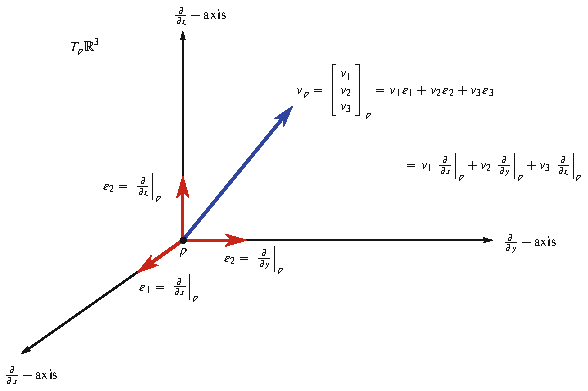
\includegraphics[width=0.960\linewidth]{images/vector/fig-2-27.pdf}
  \caption{把欧几里得向量 $e_i$ 与偏微分算子 $\partial/\partial x_i$ 等同}
  \label{fig:2-27}
\end{figure}

把这个等同付诸实践, 考虑向量
\[
v=\begin{bmatrix}2\\-3\\1\end{bmatrix}.
\]
当用欧几里得单位向量 $e_1,e_2,e_3$ 写 $v$ 时, 我们有
\[
v=2e_1-3e_2+e_3,
\]
而当用微分算子写它时, 我们有
\[
v=2\frac{\partial}{\partial x_1}-3\frac{\partial}{\partial x_2}+\frac{\partial}{\partial x_3}.
\]

从现在起我们将对 $e_1,e_2,e_3$ 与 $\frac{\partial}{\partial x_1},\frac{\partial}{\partial x_2},\frac{\partial}{\partial x_3}$ 之间作很少或不作区别, 视情况使用任何一种记号. 你还应该注意, 你可能经常看到 $\frac{\partial}{\partial x_1},\frac{\partial}{\partial x_2},\frac{\partial}{\partial x_3}$ 写为 $\partial_1,\partial_2,\partial_3$, 或 $\partial_{x_1},\partial_{x_2},\partial_{x_3}$, 甚至 $\partial_x,\partial_y,\partial_z$. 如果我们想考虑基点, 比如说
\[
v_p=\begin{bmatrix}v_1\\v_2\\v_3\end{bmatrix}_p\in T_p(\mathbb{R}^3),
\]
那么我们会写
\[
v_p=v_1\left.\frac{\partial}{\partial x_1}\right|_{p}+v_2\left.\frac{\partial}{\partial x_2}\right|_{p}+v_3\left.\frac{\partial}{\partial x_3}\right|_{p}.
\]

\section{微分 1-形式}

让我们回顾一下我们所做的. 首先我们回顾了向量空间与对偶空间. 之后我们区分了流形（流形 $\mathbb{R}^3$）与向量空间（向量空间 $\mathbb{R}^3$）, 并引入了切空间 $T_p(\mathbb{R}^3)$ 的概念, 它基本上是附着在流形 $\mathbb{R}^3$ 每个点 $p$ 上的一个向量空间 $\mathbb{R}^3$. 之后我们回顾了方向导数, 并用它们发现了向量与偏微分算子之间的一个恒等关系. 我们发现每个向量 $v_p\in T_p(\mathbb{R}^3)$ 恰好是一个微分算子
\[
v_p=\begin{bmatrix}v_1\\v_2\\v_3\end{bmatrix}_p=v_1\left.\frac{\partial}{\partial x_1}\right|_{p}+v_2\left.\frac{\partial}{\partial x_2}\right|_{p}+v_3\left.\frac{\partial}{\partial x_3}\right|_{p}.
\]
认识到每个切空间 $T_p(\mathbb{R}^n)$ 本身是一个向量空间, 显然每个切空间 $T_p(\mathbb{R}^n)$ 都有自己的对偶空间, 记为 $T_p^*(\mathbb{R}^n)$. 我们现在要看的正是这个空间.

我们现在已经准备好迎接我们一直等待的定义, 微分 1-形式的定义.

\begin{definition}[微分 1-形式]\label{def:2-4-1}
流形 $\mathbb{R}^n$ 上的微分 1-形式 $\alpha$ 是流形 $\mathbb{R}^n$ 的切向量集合上的线性泛函. 也就是说, 在流形 $\mathbb{R}^n$ 的每个点 $p$ 处, $\alpha:T_p(\mathbb{R}^n)\to\mathbb{R}$, 并且
\[
\alpha(v_p+w_p)=\alpha(v_p)+\alpha(w_p),\qquad \alpha(av_p)=a\alpha(v_p)
\]
对所有 $v_p,w_p\in T_p(\mathbb{R}^n)$ 和 $a\in\mathbb{R}$ 成立.
\end{definition}

需要做一些评注来帮助你更好地理解这个定义. 首先, 我们在讨论向量空间时已经定义了线性泛函. 向量空间所有线性泛函的集合称为该向量空间的对偶空间. 在 1-形式的定义中, 向量空间是 $T_p(\mathbb{R}^n)$. $T_p(\mathbb{R}^n)$ 的对偶空间通常记为 $T_p^*(\mathbb{R}^n)$. 因此, 我们有 $\alpha\in T_p^*(\mathbb{R}^n)$.

接下来要注意的是, 在定义中第一个所需恒等式的左边, 加法发生在向量空间 $T_p(\mathbb{R}^n)$ 中. 换句话说, $v_p+w_p\in T_p(\mathbb{R}^n)$. 等号右边的加法发生在实数集 $\mathbb{R}$ 中. 也就是说, $\alpha(v_p)+\alpha(w_p)\in\mathbb{R}$. 术语上还有一个小的怪癖：$\alpha$ 被称为流形 $\mathbb{R}^n$ 上的微分 1-形式, 尽管它的输入是向量, 即流形 $\mathbb{R}^n$ 中某个点 $p$ 处流形切空间 $T_p(\mathbb{R}^n)$ 的元素. 所以, 即使 $\alpha$ 吃进的是流形 $\mathbb{R}^n$ 的切空间 $T_p(\mathbb{R}^n)$ 的元素, 它仍被称为流形 $\mathbb{R}^n$ 上的微分 1-形式. 如果我们想指明微分形式所在的点, 我们将使用 $\alpha_p$ 或 $\alpha(p)$. 显然我们有 $\alpha_p\in T_p^*(\mathbb{R}^n)$, 即 $T_p(\mathbb{R}^n)$ 的对偶空间.

那么, 为什么叫微分 1-形式呢？加上的``1-''是因为它只把一个切向量作为输入. 后面我们将遇到 2-形式、3-形式和一般的 $k$-形式, 它们分别把两个、三个或 $k$ 个切向量作为输入. ``微分''一词是因为形式与外微分思想之间的密切关系, 我们将在后面研究. 最后, ``形式''一词是一个有点通用的数学术语, 被用于相当广泛的一类对象（双线性形式、二次形式、多重线性形式、第一和第二基本形式等等）. 因此, 微分 $k$-形式是一个数学对象, 其输入是某点处的 $k$ 个向量, 并且与某种关于微分的想法有关. 很多时候``微分''一词被省去, 微分 $k$-形式被简称为 $k$-形式. 到目前为止这个定义还有点抽象, 因此为了更好地理解, 我们现在将考虑流形 $\mathbb{R}^3$ 上一些具体而简单的 1-形式例子. 但在我们写出流形 $\mathbb{R}^3$ 上 1-形式的具体例子之前, 我们需要决定 $T_p^*(\mathbb{R}^3)$ 的一组基.

基于我们对向量空间的回顾以及那里使用的记号, 对偶基写成向量空间基的上标形式而不是下标形式. 假设我们把 $T_p(\mathbb{R}^3)$ 的基写成 $\{e_{1_p},e_{2_p},e_{3_p}\}$, 那么我们也许可以尝试把 $T_p^*(\mathbb{R}^3)$ 的基写成 $\{e_p^1,e_p^2,e_p^3\}$. 但回想标准欧几里得单位向量与微分算子之间的等同, 我们也可以把 $T_p(\mathbb{R}^3)$ 的基写成
\[
\left\{\left.\frac{\partial}{\partial x_1}\right|_{p},\left.\frac{\partial}{\partial x_2}\right|_{p},\left.\frac{\partial}{\partial x_3}\right|_{p}\right\}.
\]
但现在我们怎么写对偶基呢？我们把对偶基, 即对偶空间 $T_p^*(\mathbb{R}^3)$ 的基, 写为
\[
\{dx_{1_p},dx_{2_p},dx_{3_p}\}.
\]
是的, 这组基看起来像你在微积分中熟悉的微分. 这是有原因的. 一旦我们做了几道题, 你对这个记号更熟悉一点之后, 我们将探讨这个记号的原因. 从记号中略去基点 $p$, 我们将写
\[
\{dx_1,dx_2,dx_3\}
\]
作为与 $T(\mathbb{R}^3)$ 的基
\[
\left\{\frac{\partial}{\partial x_1},\frac{\partial}{\partial x_2},\frac{\partial}{\partial x_3}\right\}
\]
对偶的 $T^*(\mathbb{R}^3)$ 的基. 图 \ref{fig:2-28} 试图以图形方式画出流形 $\mathbb{R}^3$、点 $p$ 处的切空间 $T_p\mathbb{R}^3$ 及其对偶空间 $T_p^*\mathbb{R}^3$. 我们常常认为切空间 $T_p\mathbb{R}^3$ 和对偶空间 $T_p^*(\mathbb{R}^3)$``附着''在流形 $\mathbb{R}^3$ 的点 $p$ 上, 但我们在图中把对偶空间 $T_p^*\mathbb{R}^3$ 画在切空间 $T_p\mathbb{R}^3$ 的正上方. 对偶空间 $T_p^*\mathbb{R}^3$ 通常称为 $p$ 处的余切空间.

\begin{figure}[htbp]
  \centering
  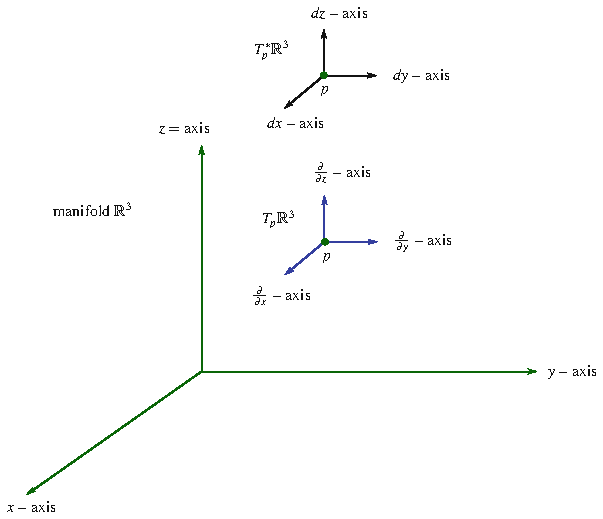
\includegraphics[width=0.715\linewidth]{images/vector/fig-2-28.pdf}
  \caption{流形 $\mathbb{R}^3$ 以及``附着''在点 $p$ 处的切空间 $T_p\mathbb{R}^3$ 的图示. 对偶空间 $T_p^*\mathbb{R}^3$ 画在它所对偶的切空间上方. 注意轴标记方式的不同}
  \label{fig:2-28}
\end{figure}

由于 $T_p^*\mathbb{R}^3$ 的任意元素都可以写成 $\{dx_1,dx_2,dx_3\}$ 的线性组合, 而 $T_p^*\mathbb{R}^3$ 的元素是 1-形式, 这当然意味着 $\mathbb{R}^3$ 上的 1-形式可以写成 $\{dx_1,dx_2,dx_3\}$ 的线性组合. 特别地, 基元素 $dx_1,dx_2,dx_3$ 本身是 $\mathbb{R}^3$ 上的 1-形式.

现在我们将确切地看到对偶基, 即 1-形式 $\{dx_1,dx_2,dx_3\}$, 如何作用于切空间基元素 $\frac{\partial}{\partial x_1},\frac{\partial}{\partial x_2},\frac{\partial}{\partial x_3}$. 由对偶基的定义, 我们有
\begin{align*}
dx_1\left(\frac{\partial}{\partial x_1}\right)=1,\qquad dx_2\left(\frac{\partial}{\partial x_1}\right)=0,\qquad dx_3\left(\frac{\partial}{\partial x_1}\right)=0, \\
dx_1\left(\frac{\partial}{\partial x_2}\right)=0,\qquad dx_2\left(\frac{\partial}{\partial x_2}\right)=1,\qquad dx_3\left(\frac{\partial}{\partial x_2}\right)=0, \\
dx_1\left(\frac{\partial}{\partial x_3}\right)=0,\qquad dx_2\left(\frac{\partial}{\partial x_3}\right)=0,\qquad dx_3\left(\frac{\partial}{\partial x_3}\right)=1.
\end{align*}

现在让我们考虑一个向量, 比如说
\[
\begin{bmatrix}-1\\3\\-4\end{bmatrix}=-\frac{\partial}{\partial x_1}+3\frac{\partial}{\partial x_2}-4\frac{\partial}{\partial x_3},
\]
看看微分形式 $dx_1,dx_2,dx_3$ 如何作用于它. 首先看 $dx_1$ 如何作用于这个向量：
\begin{align*}
dx_1\left(-\frac{\partial}{\partial x_1}+3\frac{\partial}{\partial x_2}-4\frac{\partial}{\partial x_3}\right)
&=dx_1\left(-\frac{\partial}{\partial x_1}\right)+dx_1\left(3\frac{\partial}{\partial x_2}\right)+dx_1\left(-4\frac{\partial}{\partial x_3}\right)\\
&=-dx_1\left(\frac{\partial}{\partial x_1}\right)+3dx_1\left(\frac{\partial}{\partial x_2}\right)-4dx_1\left(\frac{\partial}{\partial x_3}\right)\\
&=-1(1)+3(0)-4(0)\\
&=-1.
\end{align*}
类似地, 我们有
\begin{align*}
dx_2\left(-\frac{\partial}{\partial x_1}+3\frac{\partial}{\partial x_2}-4\frac{\partial}{\partial x_3}\right)
&=-dx_2\left(\frac{\partial}{\partial x_1}\right)+3dx_2\left(\frac{\partial}{\partial x_2}\right)-4dx_2\left(\frac{\partial}{\partial x_3}\right)\\
&=-1(0)+3(1)-4(0)\\
&=3
\end{align*}
以及
\begin{align*}
dx_3\left(-\frac{\partial}{\partial x_1}+3\frac{\partial}{\partial x_2}-4\frac{\partial}{\partial x_3}\right)
&=-dx_3\left(\frac{\partial}{\partial x_1}\right)+3dx_3\left(\frac{\partial}{\partial x_2}\right)-4dx_3\left(\frac{\partial}{\partial x_3}\right)\\
&=-1(0)+3(0)-4(1)\\
&=-4.
\end{align*}
本质上, 微分 1-形式 $dx_1,dx_2,dx_3$ 求出向量在相应轴上的投影. 回到更传统的 $x,y,z$ 记号, 1-形式 $dx$ 求出 $v_p$ 在 $\frac{\partial}{\partial x}$ 轴上的投影, 1-形式 $dy$ 求出 $v_p$ 在 $\frac{\partial}{\partial y}$ 轴上的投影, 1-形式 $dz$ 求出 $v_p$ 在 $\frac{\partial}{\partial z}$ 轴上的投影. 这在图 \ref{fig:2-29} 中作了图示.

\begin{figure}[htbp]
  \centering
  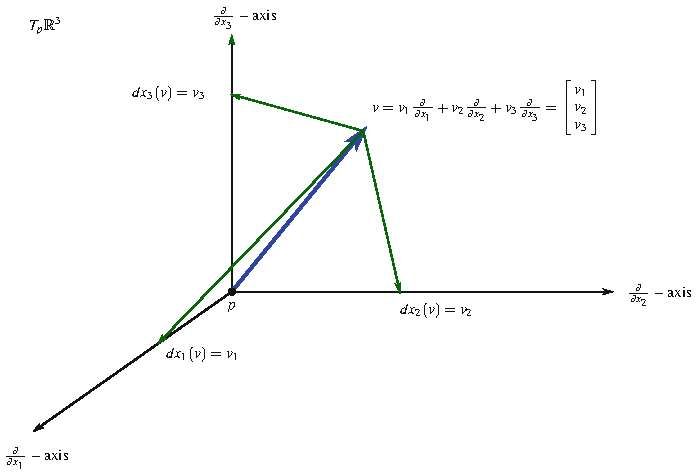
\includegraphics[width=0.845\linewidth]{images/vector/fig-2-29.pdf}
  \caption{对偶基元素如何作用于向量 $v$ 的图示. 该图在记号中没有包含点 $p$}
  \label{fig:2-29}
\end{figure}

\begin{question}\label{q:2-7}
求下列各值：
\begin{enumerate}
  \item[(a)] $dx_1\left(2\frac{\partial}{\partial x_1}+3\frac{\partial}{\partial x_1}\right)$
  \item[(b)] $dx_2\left(-\frac{\partial}{\partial x_1}+3\frac{\partial}{\partial x_2}-4\frac{\partial}{\partial x_3}\right)$
  \item[(c)] $dx_3\left(7\frac{\partial}{\partial x_2}-5\frac{\partial}{\partial x_3}\right)$
\end{enumerate}
\end{question}

由于集合 $\{dx,dy,dz\}$ 是 $T_p^*\mathbb{R}^3$ 的基, 任意元素 $\alpha\in T_p^*\mathbb{R}^3$ 都可以写成 $adx+bdy+cdz$ 的形式, 其中 $a,b,c\in\mathbb{R}$. 这些 1-形式的行为完全如你所预期. 例如, 考虑 1-形式 $2dx-3dy+5dz$ 如何作用于向量 $-\frac{\partial}{\partial x_1}+3\frac{\partial}{\partial x_2}-4\frac{\partial}{\partial x_3}$：
\begin{align*}
(2dx-3dy+5dz)\left(-\frac{\partial}{\partial x}+3\frac{\partial}{\partial y}-4\frac{\partial}{\partial z}\right)
&=2dx\left(-\frac{\partial}{\partial x}+3\frac{\partial}{\partial y}-4\frac{\partial}{\partial z}\right)\\
&\quad-3dy\left(-\frac{\partial}{\partial x}+3\frac{\partial}{\partial y}-4\frac{\partial}{\partial z}\right)\\
&\quad+5dz\left(-\frac{\partial}{\partial x}+3\frac{\partial}{\partial y}-4\frac{\partial}{\partial z}\right)\\
&=(2)(-1)(1)+(2)(3)(0)+(2)(-4)(0)\\
&\quad+(-3)(-1)(0)+(-3)(3)(1)+(-3)(-4)(0)\\
&\quad+(5)(-1)(0)+(5)(3)(0)+(5)(-4)(1)\\
&=-31.
\end{align*}
我们格外小心地展示了这个计算的每一步, 这是我们在未来当然不会总是做的.

\begin{question}\label{q:2-8}
求下列各值：
\begin{enumerate}
  \item[(a)] $(dx_1+dx_2)\left(5\frac{\partial}{\partial x_1}\right)$
  \item[(b)] $(2dx_2-3dx_3)\left(3\frac{\partial}{\partial x_1}-7\frac{\partial}{\partial x_2}+5\frac{\partial}{\partial x_3}\right)$
  \item[(c)] $(-dx_1-4dx_2+6dx_3)\left(-2\frac{\partial}{\partial x_1}+5\frac{\partial}{\partial x_2}-3\frac{\partial}{\partial x_3}\right)$
\end{enumerate}
\end{question}

为了使计算更简单, 1-形式常常写成行向量, 正如我们在向量空间的回顾中把对偶空间的元素写成行向量一样. 例如, 1-形式 $4dx_1-2dx_2+5dx_3$ 可以写成行向量 $[4,-2,5]$. 回想我们说过 $p$ 处的对偶空间常称为 $p$ 处的余切空间. 因此, 当一个 1-形式（余切空间的元素）写成行向量时, 它常被称为余向量. 这使得我们可以把上面的计算当作矩阵乘法来做. 让我们重做最后一个计算看看怎么做, 
\begin{align*}
(2dx-3dy+5dz)\left(-\frac{\partial}{\partial x}+3\frac{\partial}{\partial y}-4\frac{\partial}{\partial z}\right)
&=[2,-3,5]\begin{bmatrix}-1\\3\\-4\end{bmatrix}\\
&=(2)(-1)+(-3)(3)+(5)(-4)\\
&=-31.
\end{align*}
这当然是一个更直接的计算.

\begin{question}\label{q:2-9}
先把 1-形式写成行向量（余向量）、把向量元素写成列向量, 然后作为矩阵乘法做下列计算.
\begin{enumerate}
  \item[(a)] $(-7dx_1+dx_2)\left(2\frac{\partial}{\partial x_2}\right)$
  \item[(b)] $dx_3\left(7\frac{\partial}{\partial x_2}-5\frac{\partial}{\partial x_3}\right)$
  \item[(c)] $(2dx_2-3dx_3)\left(3\frac{\partial}{\partial x_1}-7\frac{\partial}{\partial x_2}+5\frac{\partial}{\partial x_3}\right)$
  \item[(d)] $(-dx_1-4dx_2+6dx_3)\left(-2\frac{\partial}{\partial x_1}+5\frac{\partial}{\partial x_2}-3\frac{\partial}{\partial x_3}\right)$
\end{enumerate}
\end{question}

注意我们现在有两种不同的心智图像可以用来尝试描绘微分 1-形式. 考虑图 \ref{fig:2-30}. 上面是作为行向量的微分 1-形式的图像, 这是最容易有的图像. 形如 $adx+bdy+cdz$（$a,b,c\in\mathbb{R}$）的微分 1-形式是某点处余切空间 $T_p^*\mathbb{R}^3$ 的元素, 所以把它们想象成行向量（称为余向量）是很自然的. 第二种图像是把 1-形式 $dx,dy,dz$ 看作求向量 $v_p$ 在不同轴上投影的方式. 在这种情况下, 1-形式 $adx+bdy+cdz$ 可以被看作分别按因子 $a,b,c$ 缩放相应的投影, 然后把这些不同的缩放加起来.

\begin{figure}[htbp]
  \centering
  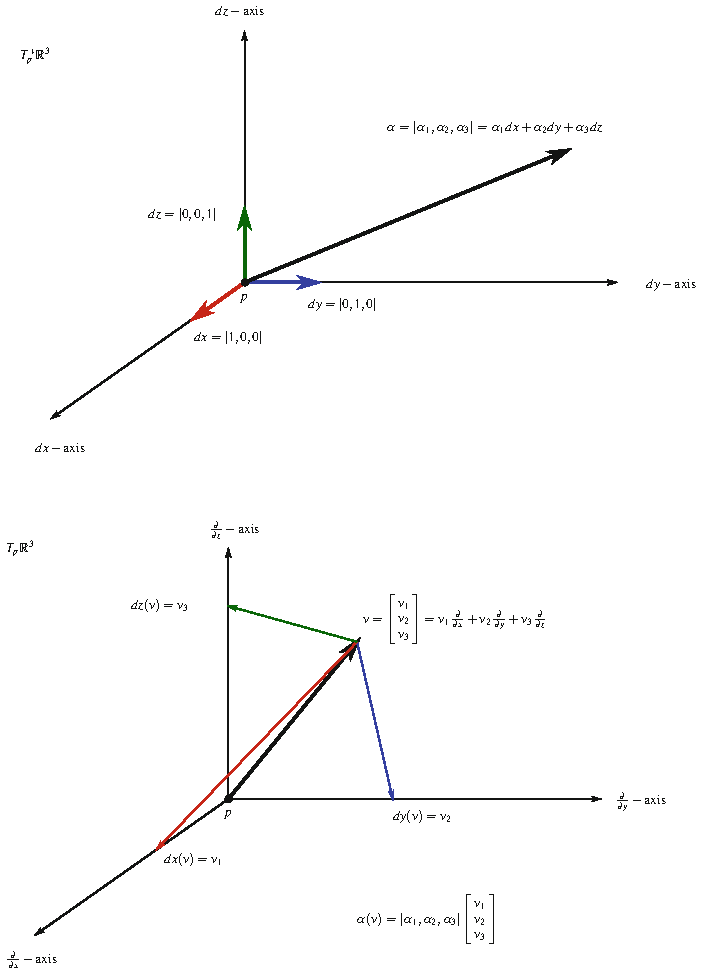
\includegraphics[width=0.896\linewidth]{images/vector/fig-2-30.pdf}
  \caption{想象或可视化微分 1-形式的两种不同方式. 作为 $T_p^*\mathbb{R}^3$ 中的余向量（上）, 或作为 $T_p\mathbb{R}^3$ 中向轴投影的线性组合（下）}
  \label{fig:2-30}
\end{figure}

在最后几道题中我们隐式地假设 1-形式和向量都在流形的同一点. 但正如向量给了我们向量场, 我们可以想象流形 $\mathbb{R}^3$ 上的 1-形式``场''. 然而实际上, 我们一般不会称它们为场, 我们只简称为 1-形式. 还记得那个有点奇怪的术语``流形 $\mathbb{R}^3$ 上的 1-形式''吗？流形上的 1-形式实际上是一个 1-形式场, 它在流形的每个点 $p$ 处给出一个特定的 1-形式, 作用于基点在该点的切向量 $v_p$.

让我们考虑一个例子. 给定流形 $\mathbb{R}^3$ 上的下列实值函数：$f(x,y,z)=x^2y$、$g(x,y,z)=\frac{x^2}{2}+yz$ 和 $h(x,y,z)=x+y+3$. 在流形 $\mathbb{R}^3$ 的每个点 $p=(x,y,z)$ 处, 通过
\[
\varphi_{(x,y,z)}=f(x,y,z)dx+g(x,y,z)dy+h(x,y,z)dz
\]
定义流形 $\mathbb{R}^3$ 上的 1-形式 $\varphi$. 流形 $\mathbb{R}^3$ 上的 1-形式 $\varphi$ 在 $\mathbb{R}^3$ 的每个点 $p$ 处定义一个不同的 1-形式. 例如, 在点 $(1,2,3)$ 处, 1-形式 $\varphi_{(1,2,3)}$ 由
\[
\varphi_{(1,2,3)}=f(1,2,3)dx+g(1,2,3)dy+h(1,2,3)dz=2dx+\frac{13}{2}dy+6dz
\]
给出. 如果我们给定向量
\[
v_p=\begin{bmatrix}2\\-1\\-2\end{bmatrix}_p
\]
在 $p=(1,2,3)$ 处, 我们将有
\begin{align*}
\varphi_p(v_p)&=\left(2dx+\frac{13}{2}dy+6dz\right)\left(2\frac{\partial}{\partial x}-1\frac{\partial}{\partial y}-2\frac{\partial}{\partial z}\right)\\
&=\left[2,\frac{13}{2},6\right]_{(1,2,3)}\begin{bmatrix}2\\-1\\-2\end{bmatrix}_{(1,2,3)}\\
&=2(2)+\frac{13}{2}(-1)+6(-2)\\
&=\frac{-29}{2}.
\end{align*}

因此, 给定流形 $\mathbb{R}^3$ 上的一个 1-形式 $\varphi$, 在 $\mathbb{R}^3$ 的每个点 $p$ 处我们都有一个映射 $\varphi_p:T_p(\mathbb{R}^3)\to\mathbb{R}$. 如果给定流形 $\mathbb{R}^3$ 上的一个向量场 $v$, 即切丛 $T\mathbb{R}^3$ 的一个截面, 那么对每个 $p\in\mathbb{R}^3$ 都有 $\varphi_p(v_p)\in\mathbb{R}$. 那么 $\varphi(v)$ 会是什么呢？注意我们没有放入一个点. 我们可以把 $\varphi(v)$ 考虑为流形 $\mathbb{R}^3$ 上的一个函数. 也就是说, 它的输入是流形上的点 $p$, 输出是实数, 像这样
\[
\varphi(v):\mathbb{R}^3\to\mathbb{R},\qquad p\longmapsto\varphi_p(v_p).
\]

\begin{question}\label{q:2-10}
对 1-形式 $\varphi_{(x,y,z)}=f(x,y,z)dx+g(x,y,z)dy+h(x,y,z)dz$, 其中 $f(x,y,z)=xy^2$、$g(x,y,z)=\frac{x^2}{3}+x$、$h(x,y,z)=xy+yz+xz$, 以及向量
\[
v_p=\begin{bmatrix}x\\x^2y\\xz\end{bmatrix}_p,
\]
求：
\begin{enumerate}
  \item[(a)] (i) $\varphi_{(-1,2,1)}$, (ii) $\varphi_{(0,-1,2)}$, (iii) $\varphi_{(8,4,-3)}$.
  \item[(b)] 求 $\varphi(v)$.
  \item[(c)] (i) 对 $p=(-1,2,1)$ 求 $\varphi_p(v_p)$；(ii) 对 $p=(0,-1,2)$ 求 $\varphi_p(v_p)$；(iii) 对 $p=(8,4,-3)$ 求 $\varphi_p(v_p)$.
\end{enumerate}
\end{question}

既然我们对 1-形式实际上做什么更熟悉了一些, 我们就准备好尝试更好地理解这个记号了. 本质上, 我们要理解我们把 $dx,dy,dz$ 记为与 $T_p(\mathbb{R}^3)$ 的基 $\frac{\partial}{\partial x},\frac{\partial}{\partial y},\frac{\partial}{\partial z}$ 对偶的 $T_p^*(\mathbb{R}^3)$ 的基的理由. 首先我们再做另一个定义, 乍一看它可能对你显得有点循环.

\begin{definition}[函数的微分]\label{def:2-4-2}
设 $f:\mathbb{R}^n\to\mathbb{R}$ 是流形 $\mathbb{R}^n$ 上的函数. $f$ 的微分 $df$ 被定义为 $\mathbb{R}^n$ 上满足如下条件的 1-形式：对所有向量 $v_p$, 
\[
df(v_p)=v_p[f].
\]
\end{definition}

让我们花一点时间考虑流形 $\mathbb{R}^3$, 试着解开并消化这一切. 首先, 给定流形 $\mathbb{R}^3$ 上的函数 $f:\mathbb{R}^3\to\mathbb{R}$ 和流形 $\mathbb{R}^3$ 中点 $p$ 处的向量 $v_p\in T_p(\mathbb{R}^3)$, 我们知道如何取这个函数在点 $p$ 处沿方向 $v_p$ 的方向导数
\[
\lim_{t\to0}\frac{f(p+tv_p)-f(p)}{t},
\]
它也可以写成
\[
\left.\frac{d}{dt}f(p+tv_p)\right|_{t=0}.
\]
然后我们认为这是用向量 $v_p$ 对给定函数 $f$ 施行一个运算, 于是为此引入了一个稍微新的记号
\[
v_p[f]=\left.\frac{d}{dt}f(p+tv_p)\right|_{t=0},
\]
反过来我们刚刚又用它定义了 $f$ 的微分, 写为 $df$, 由 $df(v_p)=v_p[f]$ 给出. 令 $p=(x_0,y_0,z_0)$, 我们把这一切放在一起得到
\begin{align*}
df(v_p)&=v_p[f]\\
&=\left.\frac{d}{dt}f(p+tv_p)\right|_{t=0}\\
&=\left.\frac{d}{dt}f(x_0+tv_1,y_0+tv_2,z_0+tv_3)\right|_{t=0}\\
&\qquad\underbrace{\qquad\qquad}_{x(t)}\quad\underbrace{\qquad\qquad}_{y(t)}\quad\underbrace{\qquad\qquad}_{z(t)}\\
&=\left.\frac{\partial f}{\partial x}\right|_{p}\cdot\left.\frac{dx(t)}{dt}\right|_{t=0}
+\left.\frac{\partial f}{\partial y}\right|_{p}\cdot\left.\frac{dy(t)}{dt}\right|_{t=0}
+\left.\frac{\partial f}{\partial z}\right|_{p}\cdot\left.\frac{dz(t)}{dt}\right|_{t=0}\\
&=\left.\frac{\partial f}{\partial x}\right|_{p}\cdot v_1+\left.\frac{\partial f}{\partial y}\right|_{p}\cdot v_2+\left.\frac{\partial f}{\partial z}\right|_{p}\cdot v_3.
\end{align*}
总之我们有
\[
df(v_p)=\left.\frac{\partial f}{\partial x}\right|_{p}\cdot v_1+\left.\frac{\partial f}{\partial y}\right|_{p}\cdot v_2+\left.\frac{\partial f}{\partial z}\right|_{p}\cdot v_3.
\]

由于这个公式对任意函数 $f:\mathbb{R}^3\to\mathbb{R}$ 都成立, 它对特殊的笛卡尔坐标函数 $x,y,z:\mathbb{R}^3\to\mathbb{R}$ 也成立. 回想笛卡尔坐标函数：若 $p\in\mathbb{R}^3$, 则 $x(p)$ 是 $p$ 的笛卡尔 $x$ 坐标值, $y(p)$ 是 $p$ 的笛卡尔 $y$ 坐标值, $z(p)$ 是 $p$ 的笛卡尔 $z$ 坐标值. 例如, 如果我们能用笛卡尔坐标把点 $p$ 写为 $(3,2,1)$, 那么 $x(p)=3$、$y(p)=2$、$z(p)=1$. 现在让我们确切地看看这些笛卡尔坐标函数每一个会发生什么. 假设
\[
v_p=\begin{bmatrix}v_1\\v_2\\v_3\end{bmatrix}_p=v_1\left.\frac{\partial}{\partial x}\right|_{p}+v_2\left.\frac{\partial}{\partial y}\right|_{p}+v_3\left.\frac{\partial}{\partial z}\right|_{p}.
\]
那么对笛卡尔坐标函数 $x:\mathbb{R}^3\to\mathbb{R}$, 我们有
\begin{align*}
dx(v_p)&=\left.\frac{\partial x}{\partial x}\right|_{p}\cdot v_1+\left.\frac{\partial x}{\partial y}\right|_{p}\cdot v_2+\left.\frac{\partial x}{\partial z}\right|_{p}\cdot v_3\\
&=(1)\cdot v_1+(0)\cdot v_2+(0)\cdot v_3\\
&=v_1.
\end{align*}
但当我们写 $\frac{\partial x}{\partial x}$ 时是什么意思呢？分子中的 $x$ 是笛卡尔坐标函数, 而分母中的 $x$ 表示我们对其求导的变量. 因此 $\frac{\partial x}{\partial x}$ 给出笛卡尔坐标函数 $x$ 在 $x$ 方向的变化率.

\begin{question}\label{q:2-11}
解释笛卡尔坐标函数 $x$ 在 $x$ 方向的变化率确实是一, 从而证明 $\frac{\partial x}{\partial x}=1$. 考虑当点 $p$ 在 $x$ 方向移动时 $x(p)$ 如何变化, 可能会有所帮助. 笛卡尔坐标函数 $x$ 在 $y$ 和 $z$ 方向的变化率是多少？解释你的答案如何证明 $\frac{\partial x}{\partial y}=0$ 和 $\frac{\partial x}{\partial z}=0$.
\end{question}

类似地, 我们有
\begin{align*}
dy(v_p)&=\left.\frac{\partial y}{\partial x}\right|_{p}\cdot v_1+\left.\frac{\partial y}{\partial y}\right|_{p}\cdot v_2+\left.\frac{\partial y}{\partial z}\right|_{p}\cdot v_3\\
&=(0)\cdot v_1+(1)\cdot v_2+(0)\cdot v_3\\
&=v_2
\end{align*}
以及
\begin{align*}
dz(v_p)&=\left.\frac{\partial z}{\partial x}\right|_{p}\cdot v_1+\left.\frac{\partial z}{\partial y}\right|_{p}\cdot v_2+\left.\frac{\partial z}{\partial z}\right|_{p}\cdot v_3\\
&=(0)\cdot v_1+(0)\cdot v_2+(1)\cdot v_3\\
&=v_3.
\end{align*}

\begin{question}\label{q:2-12}
求笛卡尔坐标函数 $y$ 在 $x,y,z$ 方向的变化率, 并用它证明 $\frac{\partial y}{\partial x}=0$、$\frac{\partial y}{\partial y}=1$、$\frac{\partial y}{\partial z}=0$. 然后求笛卡尔坐标函数 $z$ 在 $x,y,z$ 方向的变化率, 证明 $\frac{\partial z}{\partial x}=0$、$\frac{\partial z}{\partial y}=0$、$\frac{\partial z}{\partial z}=1$.
\end{question}

\begin{question}\label{q:2-13}
把 $e_1=\frac{\partial}{\partial x}$、$e_2=\frac{\partial}{\partial y}$、$e_3=\frac{\partial}{\partial z}$ 写出来, 证明笛卡尔坐标函数的微分 $dx,dy,dz$ 给出
\begin{align*}
dx\left(\frac{\partial}{\partial x}\right)=1,\quad dy\left(\frac{\partial}{\partial x}\right)=0,\quad dz\left(\frac{\partial}{\partial x}\right)=0, \\
dx\left(\frac{\partial}{\partial y}\right)=0,\quad dy\left(\frac{\partial}{\partial y}\right)=1,\quad dz\left(\frac{\partial}{\partial y}\right)=0, \\
dx\left(\frac{\partial}{\partial z}\right)=0,\quad dy\left(\frac{\partial}{\partial z}\right)=0,\quad dz\left(\frac{\partial}{\partial z}\right)=1.
\end{align*}
\end{question}

现在我们可以比较笛卡尔坐标函数 $x,y,z$ 的微分 $dx,dy,dz$ 的行为与对偶基元素（即 $T_p(\mathbb{R}^3)$ 的基元素 $\frac{\partial}{\partial x},\frac{\partial}{\partial y},\frac{\partial}{\partial z}$ 的对偶）的行为. 我们看到它们的行为完全相同. 这解释了本节开头对偶基元素的记号选择. 对偶基元素恰恰是笛卡尔坐标函数的微分.

给定一个具体的函数 $f$, 我们想知道如何实际写出微分 $df$. 假设 $f:\mathbb{R}^3\to\mathbb{R}$ 是流形 $\mathbb{R}^3$ 上的函数, $v_p$ 是任意点处的任意向量. 由于
\[
df(v_p)=\left.\frac{\partial f}{\partial x}\right|_{p}\cdot v_1+\left.\frac{\partial f}{\partial y}\right|_{p}\cdot v_2+\left.\frac{\partial f}{\partial z}\right|_{p}\cdot v_3
\]
且
\[
v_1=dx(v_p),\qquad v_2=dy(v_p),\qquad v_3=dz(v_p),
\]
我们把这些放在一起得到
\begin{align*}
df(v_p)&=\left.\frac{\partial f}{\partial x}\right|_{p}\cdot v_1+\left.\frac{\partial f}{\partial y}\right|_{p}\cdot v_2+\left.\frac{\partial f}{\partial z}\right|_{p}\cdot v_3\\
&=\left.\frac{\partial f}{\partial x}\right|_{p}\cdot dx(v_p)+\left.\frac{\partial f}{\partial y}\right|_{p}\cdot dy(v_p)+\left.\frac{\partial f}{\partial z}\right|_{p}\cdot dz(v_p)\\
&=\left(\left.\frac{\partial f}{\partial x}\right|_{p}dx+\left.\frac{\partial f}{\partial y}\right|_{p}dy+\left.\frac{\partial f}{\partial z}\right|_{p}dz\right)(v_p)
\end{align*}
于是我们有
\[
df=\left.\frac{\partial f}{\partial x}\right|_{p}dx+\left.\frac{\partial f}{\partial y}\right|_{p}dy+\left.\frac{\partial f}{\partial z}\right|_{p}dz.
\]
我们把函数 $f$ 的微分写成对偶基元素的线性组合, 从而证明了 $df\in T_p^*(\mathbb{R}^3)$. 函数 $f$ 的微分是一个 1-形式.

我们最后要做的是考虑思考函数 $f$ 的微分 $df$ 的另一种方式. 为了画必要的图, 我们将考虑流形 $\mathbb{R}^2$, 因为我们可以用三维方式画函数 $f:\mathbb{R}^2\to\mathbb{R}$ 的图像, 而恰当地画函数 $f:\mathbb{R}^3\to\mathbb{R}$ 的图像需要四个维度, 但对所有函数 $f:\mathbb{R}^n\to\mathbb{R}$ 的基本思想是相同的. 令 $v=\binom{v_1}{v_2}$, 我们有
\begin{align*}
v[f]&=\left(v_1\frac{\partial}{\partial x}+v_2\frac{\partial}{\partial y}\right)[f]\\
&=\frac{\partial f}{\partial x}v_1+\frac{\partial f}{\partial y}v_2\\
&=\frac{\partial f}{\partial x}dx(v)+\frac{\partial f}{\partial y}dy(v)\\
&=\left(\frac{\partial f}{\partial x}dx+\frac{\partial f}{\partial y}dy\right)(v)\\
&=df(v).
\end{align*}

\begin{question}\label{q:2-14}
把基点放回记号中重做上面的计算. $f$ 在 $p$ 处的微分既可以写成 $df_p$, 也可以写成 $df(p)$.
\end{question}

但现在真正的问题是, 这个 $f$ 的微分 $df$ 到底是什么？关键在图 \ref{fig:2-31} 中. $f$ 的微分 $df$ 吃进一个位于流形 $\mathbb{R}^2$ 的某点 $p$ 处的向量 $v_p$, 并给出一个数, 即当你从 $p$ 沿着 $v_p$ 移动时, 函数 $f$ 图像切平面的``rise''. 这个输出也可以被看作切平面上的一个点. 因此, 在某种意义上, $df$``编码''了当你沿着以 $p$ 为基点的不同向量移动时函数 $f$ 的切平面中发生的``rise''. 这应该不令人惊讶. $f(x,y)$ 在点 $(x_0,y_0)$ 处切平面 $T$ 的公式由
\[
T(x,y)=f(x_0,y_0)+\left.\frac{\partial f}{\partial x}\right|_{(x_0,y_0)}\cdot(x-x_0)+\left.\frac{\partial f}{\partial y}\right|_{(x_0,y_0)}\cdot(y-y_0)
\]
给出.

\begin{figure}[htbp]
  \centering
  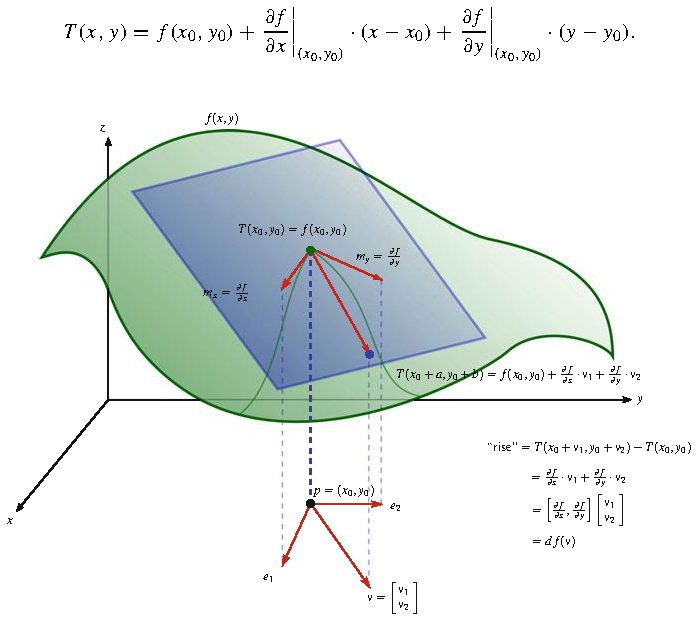
\includegraphics[width=0.960\linewidth]{images/vector/fig-2-31.pdf}
  \caption{微分 $df_p$ 是函数 $f$ 在点 $p$ 处的线性逼近. 换句话说, 微分 $df_p$``编码''了 $f$ 在 $p$ 处的切平面}
  \label{fig:2-31}
\end{figure}

如图所表明的, 给定向量 $v=\binom{v_1}{v_2}_p$, 这个向量的终点（在 $\mathbb{R}^2$ 中）是 $(x_0+v_1,y_0+v_2)$. $f$ 的切平面（在点 $p=(x_0,y_0)$ 处）中位于 $(x_0+v_1,y_0+v_2)$ 正上方的点由
\begin{align*}
T(x_0+v_1,y_0+v_2)
&=f(x_0,y_0)+\left.\frac{\partial f}{\partial x}\right|_{(x_0,y_0)}\cdot(x_0+v_1-x_0)+\left.\frac{\partial f}{\partial y}\right|_{(x_0,y_0)}\cdot(y_0+v_2-y_0)\\
&=f(x_0,y_0)+\left.\frac{\partial f}{\partial x}\right|_{(x_0,y_0)}\cdot v_1+\left.\frac{\partial f}{\partial y}\right|_{(x_0,y_0)}\cdot v_2
\end{align*}
给出, 所以切平面中从 $f(x_0,y_0)$ 起的``rise''由
\begin{align*}
\text{``rise''}&=T(x_0+v_1,y_0+v_2)-T(x_0,y_0)\\
&=f(x_0,y_0)+\left.\frac{\partial f}{\partial x}\right|_{(x_0,y_0)}\cdot v_1+\left.\frac{\partial f}{\partial y}\right|_{(x_0,y_0)}\cdot v_2-f(x_0,y_0)\\
&=\left.\frac{\partial f}{\partial x}\right|_{(x_0,y_0)}\cdot v_1+\left.\frac{\partial f}{\partial y}\right|_{(x_0,y_0)}\cdot v_2\\
&=df_p(v_p)
\end{align*}
给出. 因此, $f$ 在 $p$ 处的微分 $df_p$ 给出当你沿着向量 $v_p$ 移动时 $f$ 在 $p$ 处切平面的``rise'', 它本质上编码了这个切平面如何行为. 切平面是 $f$ 在 $p$ 处最接近的线性逼近, 所以本质上 $df_p$ 可以被想成函数 $f$ 在点 $p$ 处的线性逼近.

作为最后一个评注, 写成行向量的微分 1-形式 $df$
\[
df=\frac{\partial f}{\partial x}dx+\frac{\partial f}{\partial y}dy=\left(\frac{\partial f}{\partial x},\frac{\partial f}{\partial y}\right)
\]
（在 $\mathbb{R}^2$ 情形中）或
\[
df=\frac{\partial f}{\partial x}dx+\frac{\partial f}{\partial y}dy+\frac{\partial f}{\partial z}dz=\left(\frac{\partial f}{\partial x},\frac{\partial f}{\partial y},\frac{\partial f}{\partial z}\right)
\]
（在 $\mathbb{R}^3$ 情形中）是否让你想起向量微积分中的什么东西？它应该让你想起 $\mathrm{grad}(f)$ 或 $\nabla(f)$. 事实上, $df$ 和 $\mathrm{grad}(f)$ 密切相关. 我们将在第 9 章探讨这一关系.

我们现在考虑几个例子. 设 $f:\mathbb{R}^3\to\mathbb{R}$ 由 $f(x,y,z)=x^2y^3z$ 给出, 并考虑每个点 $p=(x,y,z)\in\mathbb{R}^3$ 处的向量 $v_p=\begin{bmatrix}1\\2\\3\end{bmatrix}_p$. 首先求 $df(v_p)$. 由于 $v_p$ 在每个点 $p$ 都相同, 我们可以从记号中略去 $p$. 我们有
\begin{align*}
df(v)&=v[f]\\
&=\left(\frac{\partial}{\partial x}+2\frac{\partial}{\partial y}+3\frac{\partial}{\partial z}\right)\left(x^2y^3z\right)\\
&=\frac{\partial(x^2y^3z)}{\partial x}+2\frac{\partial(x^2y^3z)}{\partial y}+3\frac{\partial(x^2y^3z)}{\partial z}\\
&=2xy^3z+2(3x^2y^2z)+3(x^2y^3).
\end{align*}
现在假设我们给定具体点 $p=(-1,2,-2)$. 在 $p=(-1,2,-2)$ 处求 $df(v_p)$ 只需要代入数值
\[
df(v_p)=2(-1)^2(2)^3(-2)+2\bigl(3(-1)^2(2)^2(-2)\bigr)+3(-1)^2(2)^3=8.
\]

\begin{question}\label{q:2-15}
设 $f(x,y,z)=(x^2-1)y+(y^2+2)z$.
\begin{enumerate}
  \item[(i)] 求 $df$.
  \item[(ii)] 令 $v_p=\begin{bmatrix}v_1\\v_2\\v_3\end{bmatrix}_{(p_1,p_2,p_3)}$. 求 $df(v_p)$.
  \item[(iii)] 令 $v_p=\begin{bmatrix}-2\\1\\3\end{bmatrix}_{(-1,0,2)}$. 求 $df(v_p)$.
\end{enumerate}
\end{question}

\begin{question}\label{q:2-16}
设 $f$ 和 $g$ 是 $\mathbb{R}^3$ 上的函数. 证明 $d(fg)=gdf+fdg$.
\end{question}

\begin{question}\label{q:2-17}
设 $f:\mathbb{R}^3\to\mathbb{R}$、$h:\mathbb{R}\to\mathbb{R}$ 和 $h(f):\mathbb{R}^3\to\mathbb{R}$ 都有定义. 证明 $d(h(f))=h'(f)df$.
\end{question}

\section{小结、参考文献与问题}

\subsection{小结}

因为这一区别对更抽象的空间很重要, 我们首先大谈特谈 $\mathbb{R}^n$ 中点的集合是流形 $\mathbb{R}^n$, 而 $\mathbb{R}^n$ 中向量的集合是向量空间 $\mathbb{R}^n$. 然后我们定义了笛卡尔函数 $x_i:\mathbb{R}^n\to\mathbb{R}$, 它把流形 $\mathbb{R}^n$ 中的点 $p$ 送到其第 $i$ 个坐标值.

$n$ 维流形 $M$ 在点 $p\in M$ 处的切空间被引入为 $M$ 在点 $p$ 处所有切向量的空间, 记为 $T_pM$. 切空间 $T_pM$ 本质上可以被看作附着在 $M$ 的点 $p$ 处的向量空间 $\mathbb{R}^n$ 的一个副本. 流形的所有切空间的集合称为切丛, 记为 $TM$. 向量场被定义为一个函数 $v$, 它给 $M$ 的每个点 $p$ 指派 $T_pM$ 的一个元素 $v_p$. 向量场有时被称为切丛的截面.

函数 $f:M\to\mathbb{R}$ 在点 $p$ 处沿方向 $v_p$ 的方向导数被定义为
\[
v_p[f]\equiv\left.\frac{d}{dt}f(p+tv_p)\right|_{t=0},
\]
这与向量微积分中的定义完全相同, 只是去掉了 $v_p$ 必须是单位向量的要求. 去掉这一要求略微改变了方向导数的几何意义, 但使我们能够保留简单的公式
\[
v_p[f]=\sum_{i=1}^{n}v_i\cdot\left.\frac{\partial f}{\partial x_i}\right|_{p_i}\qquad\text{其中}\qquad
v_p=\begin{bmatrix}v_1\\v_2\\\vdots\\v_n\end{bmatrix}.
\]
这个公式随后被用来做出最有用和最出人意料的等同之一, 
\begin{center}
\fbox{\parbox{0.86\textwidth}{\centering
欧几里得向量 $e_i$ 可以与偏微分算子 $\dfrac{\partial}{\partial x_i}$ 等同
}}
\end{center}
换句话说, 我们把欧几里得向量 $e_i$ 想成就是偏微分算子 $\frac{\partial}{\partial x_i}$.

这个方向导数随后被用来定义与函数 $f$ 相联系的一个特定线性泛函, 
\[
df(v_p)=v_p[f].
\]
这个线性泛函称为 $f$ 的微分. 由于 $v_p\in T_pM$, 而 $T_pM$ 是一个向量空间, 线性泛函 $df$ 在 $T_pM$ 的对偶空间中, 这个对偶空间称为余切空间. 我们写 $df\in T_p^*M$. 此外, 可以用笛卡尔坐标函数 $x_i$ 定义微分 $dx_i$, 事实证明它们是与 $T_pM$ 的欧几里得基对偶的 $T_p^*M$ 的基. 因此, 利用上面的等同, 我们有 $\{\frac{\partial}{\partial x_1},\ldots,\frac{\partial}{\partial x_n}\}$ 作为 $T_pM$ 的标准基, $\{dx_1,\ldots,dx_n\}$ 作为 $T_p^*M$ 的标准对偶基. $T_p^*M$ 的元素也称为微分 1-形式. 微分 1-形式 $dx_i$ 的行为类似于笛卡尔坐标函数, 挑出向量 $v_p$ 的第 $i$ 个分量, 即 $dx_i(v_p)=v_i$. 在几何上, 我们可以把 $dx_i$ 想成求 $v_p$ 在第 $i$ 个轴上的投影向量的长度.

\subsection{参考文献与进一步阅读}

向量和向量场出现在多元微积分的各个角落, 例如见 Stewart~\cite{ref43}, 甚至 Marsden 和 Hoffman~\cite{ref31}, 但切空间和切丛通常不会在这一层次遇到或明确化. 那通常留给更高级的课程, 常常是微分几何. 对这一材料有相当多有趣而严谨的导引. 仅举几例, Munkres~\cite{ref35}、O'Neill~\cite{ref36}、Tu~\cite{ref46}、Spivak~\cite{ref41} 和 Thorpe~\cite{ref45} 都是流形上分析与微分几何的好导引, 因此都包含关于切空间和切丛的出色论述. 同样, Stewart~\cite{ref43} 和 Marsden 与 Hoffman~\cite{ref31} 是方向导数和多元微积分的优秀参考书. 本章还通过考察微分 1-形式, 开始了对微分形式的温和导引, 这将用几章来完成. 本章关于微分 1-形式的材料大体上遵循了 Bachman~\cite{ref04} 和 O'Neill~\cite{ref36} 的精神, 不过也参考了 Munkres~\cite{ref35}、Edwards~\cite{ref18} 和 Martin~\cite{ref33}.

\subsection{问题}

\begin{question}\label{q:2-18}
令 $p_1=(2,9,-2)$、$p_2=(1,0,-3)$、$p_3=(12,-7,4)$ 是 $\mathbb{R}^3$ 中的点, 令 $x,y,z$ 是 $\mathbb{R}^3$ 上的笛卡尔坐标函数. 求
\begin{gather*}
\text{a) }x(p_1),\quad \text{d) }x(p_2),\quad \text{g) }x(p_3),\\
\text{b) }y(p_1),\quad \text{e) }y(p_2),\quad \text{h) }y(p_3),\\
\text{c) }z(p_1),\quad \text{f) }z(p_2),\quad \text{i) }z(p_3).
\end{gather*}
\end{question}

\begin{question}\label{q:2-19}
考虑流形 $\mathbb{R}^3$ 和向量场 $v=xye_1+\bigl(z-x^3\bigr)e_2-(x+z-4)e_3$, 其中 $e_1,e_2,e_3$ 是欧几里得向量. 若 $p_1=(1,-3,2)$、$p_2=(0,1,4)$、$p_3=(-5,-2,2)$, 求向量 $v_{p_1},v_{p_2},v_{p_3}$. 这些向量各在什么空间中？
\end{question}

\begin{question}\label{q:2-20}
求 $f(x,y)=5x^2y-4xy^3$ 在方向 $v_1=\binom{5}{12}$ 和 $v_2=\frac{1}{13}\binom{5}{12}$ 上、在点 $(1,2)$ 处的方向导数. 解释 $D_{v_1}f$ 与 $D_{v_2}f$ 之间的差别.
\end{question}

\begin{question}\label{q:2-21}
求 $f(x,y)=x\ln(y)$ 在方向 $v_1=\binom{-4}{3}$ 和 $v_2=\frac{1}{5}\binom{-4}{3}$ 上、在点 $(1,-3)$ 处的方向导数. 解释 $D_{v_1}f$ 与 $D_{v_2}f$ 之间的差别.
\end{question}

\begin{question}\label{q:2-22}
求 $f(x,y,z)=xe^{yz}$ 在方向 $v_1=\begin{bmatrix}2\\-2\\1\end{bmatrix}$ 和 $v_2=\frac{1}{3}\begin{bmatrix}2\\-2\\1\end{bmatrix}$ 上、在点 $(3,0,2)$ 处的方向导数. 解释 $D_{v_1}f$ 与 $D_{v_2}f$ 之间的差别.
\end{question}

\begin{question}\label{q:2-23}
给定 $f(x,y,z)=\sqrt{x+yz}$ 和 $v=2\frac{\partial}{\partial x}+3\frac{\partial}{\partial y}+6\frac{\partial}{\partial z}$, 求 $v[f]$ 在点 $(1,3,1)$ 处的值.
\end{question}

\begin{question}\label{q:2-24}
给定 $f(x,y,z)=xe^y+ye^z+ze^x$ 和 $v=5\frac{\partial}{\partial x}+1\frac{\partial}{\partial y}-2\frac{\partial}{\partial z}$, 求 $v[f]$ 在点 $(0,0,0)$ 处的值.
\end{question}

\begin{question}\label{q:2-25}
给定 $f(x,y,z)=\sqrt{xyz}$ 和 $v=-1\frac{\partial}{\partial x}-2\frac{\partial}{\partial y}+2\frac{\partial}{\partial z}$, 求 $v[f]$ 在点 $(3,2,6)$ 处的值.
\end{question}

\begin{question}\label{q:2-26}
给定 $f(x,y,z)=x+y^2+z^3$ 和 $v=-3\frac{\partial}{\partial x}+4\frac{\partial}{\partial y}-2\frac{\partial}{\partial z}$, 求 $v[f]$ 在点 $(2,5,-1)$ 处的值.
\end{question}

\begin{question}\label{q:2-27}
给定流形 $\mathbb{R}^3$ 上的 1-形式 $\alpha=(x^3+2yz^2)dx+(xy-2)dy+x^4dz$, 对 $p_1=(-1,3,2)$、$p_2=(2,-2,1)$、$p_3=(3,-5,-2)$ 求 1-形式 $\alpha_{p_i}$.
\end{question}

\begin{question}\label{q:2-28}
给定流形 $\mathbb{R}^3$ 上的 1-形式 $\alpha=(x^3-2yz^2)dx+dy+x^4dz$, 对 $p_1=(-1,3,2)$、$p_2=(2,-2,1)$、$p_3=(3,-5,-2)$ 求 1-形式 $\alpha_{p_i}$.
\end{question}

\begin{question}\label{q:2-29}
给定 $\mathbb{R}^3$ 上的 1-形式 $\alpha=(x^3+2yz^2)dx+(xy-2)dy+x^4dz$ 和 $\beta=(x^3-2yz^2)dx+dy+x^4dz$, 求 1-形式 $\alpha+\beta$ 和 $\alpha-\beta$. 然后对上一题中的点 $p_i$ 求 $(\alpha+\beta)_{p_i}$ 和 $(\alpha-\beta)_{p_i}$.
\end{question}

\begin{question}\label{q:2-30}
给定 1-形式 $\alpha=x^3dx-xyzdy+y^2dz$, 求 1-形式 $2\alpha$ 和 $\frac13\alpha$.
\end{question}

\begin{question}\label{q:2-31}
给定 1-形式 $\omega=\frac{xy}{2}dx-\sqrt{yz}dy+(x+z)^\frac23dz$ 和 $p=(2,-1,3)$, 对下列向量求 $\alpha_p(v_p)$：
\begin{enumerate}
  \item[(a)] $\begin{bmatrix}2\\-2\\1\end{bmatrix}$
  \item[(b)] $\begin{bmatrix}1\\3\\-5\end{bmatrix}$
  \item[(c)] $\begin{bmatrix}x+y\\z-2\\xz\end{bmatrix}$
  \item[(d)] $4e_1+7e_2-3e_3$
  \item[(e)] $\frac12e_1+\frac74e_2-\frac35e_3$
  \item[(f)] $-\sqrt{xy}e_1+\sqrt{xz}e_2-3ye_3$
  \item[(g)] $2\frac{\partial}{\partial x}-3\frac{\partial}{\partial y}+4\frac{\partial}{\partial z}$
  \item[(h)] $-2\frac{\partial}{\partial x}+\frac53\frac{\partial}{\partial y}+\frac{\partial}{\partial z}$
  \item[(i)] $\sqrt{x+y+z}\frac{\partial}{\partial x}-\sqrt{x}\ln(y)\frac{\partial}{\partial y}+\sqrt{zy}\frac{\partial}{\partial z}$
\end{enumerate}
\end{question}

\begin{question}\label{q:2-32}
求下列函数的微分 $df$：
\begin{enumerate}
  \item[(a)] $f(x,y)=x^2y^3$
  \item[(b)] $f(x,y)=x^2+y^2$
  \item[(c)] $f(x,y)=x+y^3$
  \item[(d)] $f(x,y,z)=x^2+y^3+z^4$
  \item[(e)] $f(x,y,z)=\sqrt{xyz}$
  \item[(f)] $f(x,y,z)=xe^y+ye^z+ze^x$
  \item[(g)] $f(x,y,z)=\sqrt{x+yz}$
  \item[(h)] $f(x,y,z)=x\ln(y)+y\ln(z)+z\ln(x)$
  \item[(i)] $f(x,y,z)=\left(x^3+y^3+z^3\right)^\frac23$
\end{enumerate}
\end{question}

\begin{question}\label{q:2-33}
对你在上一题中求出的微分以及上一题之前的题中的向量, 在点 $p=(2,-1,3)$ 处求 $df[v_p]$.
\end{question}

% 第 3 章 楔积
\chapter{楔积}

本章我们引入一种``相乘''1-形式的方法，称为\newterm{wedge-product}{楔积}{wedge product}. 把两个 1-形式楔乘在一起，就得到 2-形式；把三个 1-形式楔乘在一起，就得到 3-形式；以此类推. 第 1 节解释楔积的几何意义以及如何计算它. 第 2 节引入一般的 2-形式、3-形式与 $k$-形式，并探讨它们背后的几何. 第 3 节深入探讨楔积的代数性质以及若干不同的楔积公式. 不同的书以不同的方式引入楔积. 这些公式中常常有一些被作为楔积的定义给出. 然而这样做会掩盖楔积背后的几何意义，这正是本书采取不同方法的原因.

第 4 节相当简短，只是引入一种称为内积的东西，并证明若干联系内积与楔积的恒等式. 我们以后会需要这些恒等式，但由于它们依赖楔积，因此现在正是引入并证明它们的恰当时机.

\section{用楔积求面积与体积}

我们以一个重要的观点开始本章. 考虑流形 $\mathbb{R}^n$. 流形 $\mathbb{R}^n$ 的每个点 $p$ 处都有一个切空间 $T_p\mathbb{R}^n$，它是一个与向量空间 $\mathbb{R}^n$ 同构的向量空间. 若存在一一且映上的映射 $\varphi:V\to W$，使得对 $v_1,v_2,v\in V$ 与 $c\in\mathbb{R}$ 有
\begin{enumerate}
  \item $\varphi(v_1+v_2)=\varphi(v_1)+\varphi(v_2)$，
  \item $\varphi(cv)=c\varphi(v)$，
\end{enumerate}
则两个向量空间 $V$ 与 $W$ 称为同构的，记为 $V\simeq W$.

这不是一门抽象代数课程，所以我们不想在同构上做太多文章，只想强调：如果两个向量空间同构，我们就可以把它们本质上想成同一个向量空间的两份拷贝. 就 $\mathbb{R}^n$ 而言，其底流形本身也是一个向量空间，它与每个点处的切空间同构.

当我们最终遇到更一般的流形而不是由向量空间 $\mathbb{R}^n$ 给出的流形时，区分底流形与向量空间这一点极其重要. 这最终也将帮助我们把所有向量微积分放进一个更广阔的背景下. 向量微积分是一门强有力的学科，但它隐式地建立在 $\mathbb{R}^3$ 上，而对流形 $\mathbb{R}^3$ 有
\[
\text{流形 }\mathbb{R}^3\simeq T_p\mathbb{R}^3\simeq T_p^*\mathbb{R}^3\simeq \text{向量空间 }\mathbb{R}^3.
\]
这些在向量微积分中从未被明确指出的同构，正是让你能够把向量想成位于流形 $\mathbb{R}^3$ 内部、从而能够取方向导数的东西. 由于这些同构，所有这些空间都被相当草率而不精确地混在一起合并使用. 转向更一般的流形需要我们把这些差别一一剥离出来并加以理解，这是本书的一个主要目标.

\begin{figure}[htbp]
  \centering
  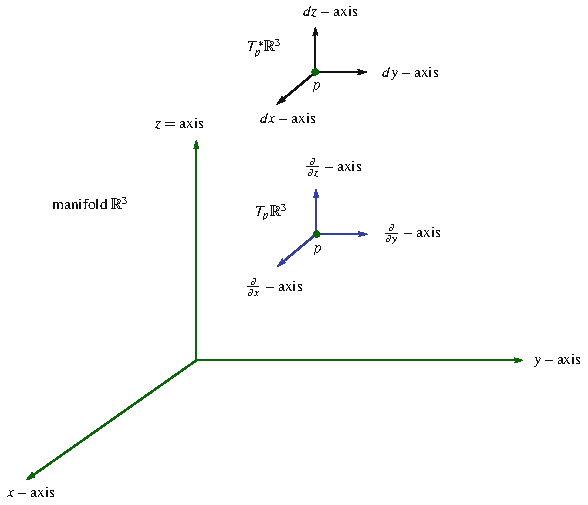
\includegraphics[width=0.715\linewidth]{images/vector/fig-3-1.pdf}
  \caption{流形 $\mathbb{R}^3$、切空间 $T_p\mathbb{R}^3$ 与余切空间 $T_p^*\mathbb{R}^3$ 一起画出. 尽管余切空间 $T_p^*\mathbb{R}^3$ 实际上与切空间 $T_p\mathbb{R}^3$ 一样附着在流形的同一点 $p$ 处，但这里把它画在切空间的上方. 本书将大体遵循这一约定}
  \label{fig:3-1}
\end{figure}

在上一章我们还发现，每个点 $p$ 处的切空间 $T_p\mathbb{R}^n$ 有一组基
\[
\left\{\left.\frac{\partial}{\partial x_1}\right|_p,\;\left.\frac{\partial}{\partial x_2}\right|_p,\ldots,\left.\frac{\partial}{\partial x_n}\right|_p\right\}
\]
并且每个点 $p$ 处有一个余切空间 $T_p^*\mathbb{R}^n$，它是向量空间 $T_p\mathbb{R}^n$ 的对偶空间，有一组基
\[
\{dx_1(p),dx_2(p),\ldots,dx_n(p)\}
\]
如果记号中省略基点 $p$，就简写为 $\{dx_1,dx_2,\ldots,dx_n\}$. 到目前为止我们建立起来的图像如图 \ref{fig:3-1} 所示，图中画出了流形 $\mathbb{R}^3$ 及其上叠加的切空间 $T_p\mathbb{R}^3$. 余切空间 $T_p^*\mathbb{R}^3$ 画在切空间的上方.

1-形式 $dx_1(p),dx_2(p),\ldots,dx_n(p)$ 恰好就是向量空间 $T_p\mathbb{R}^n$ 上的线性泛函. 与上面一致，我们有 $T_p\mathbb{R}^n\simeq\mathbb{R}^n$，其中 $T_p\mathbb{R}^n$ 的元素 $v_p$ 通常写成列向量；而 $T_p^*\mathbb{R}^n\simeq\mathbb{R}^n$，其中 $T_p^*\mathbb{R}^n$ 的元素 $\alpha_p$ 常写成行向量并称为余向量. 因此，我们可以用矩阵乘法（行向量乘以列向量）来表示 1-形式 $\alpha_p$ 作用于向量 $v_p$，即 $\alpha_p(v_p)$. 现在我们再引入一点点记号. 这有时也被写为
\[
\alpha_p(v_p)=\langle\alpha_p,v_p\rangle=\langle\alpha,v\rangle_p.
\]
因此，尖括号 $\langle\cdot,\cdot\rangle$ 表示微分形式与向量之间的\newterm{canonical-pairing}{典范配对}{canonical pairing}. 有时作者甚至不在乎典范配对中的顺序，你甚至偶尔会看到 $\langle v_p,\alpha_p\rangle$. 有些微积分教材用尖括号表示行向量；我们在这里不使用那种记号.

点 $p$ 处的微分 1-形式就是 $T_p^*\mathbb{R}^n$ 的一个元素. 我们的目标是弄清楚如何把 1-形式相乘而得到 2-形式、3-形式与 $k$-形式. 我们希望以一种能保持某些与体积有关的性质的方式来相乘微分 1-形式. （这一点一会儿就会更清楚.）

暂时我们将在流形 $\mathbb{R}^3$ 上工作，因为相关的图更容易画出. 然后我们将转向 $\mathbb{R}^2$，甚至 $\mathbb{R}$，最后再转向更一般的 $\mathbb{R}^n$ 情形. 首先我们回顾上一章所学的内容. 图 \ref{fig:3-2} 展示了线性泛函，即对偶基元素 $dx_1,dx_2,dx_3$（即 $dx,dy,dz$）对向量 $v_p\in T_p\mathbb{R}^3$ 做了什么；它们求出 $v_p$ 在 $T_p\mathbb{R}^3$ 的各坐标轴上的投影. 一般地，基点 $p$ 在记号中大部分时候被省略.

\begin{figure}[htbp]
  \centering
  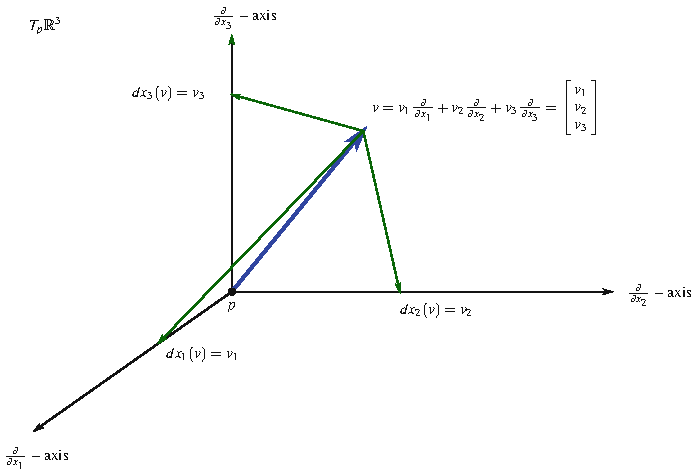
\includegraphics[width=0.845\linewidth]{images/vector/fig-3-2.pdf}
  \caption{对偶基元素如何作用于向量 $v$ 的示意图. 图中记号省略了点 $p$}
  \label{fig:3-2}
\end{figure}

图 \ref{fig:3-3} 的上方把 1-形式 $\alpha=\alpha_1dx+\alpha_2dy+\alpha_3dz$ 作为余切空间 $T_p^*\mathbb{R}^3$ 的一个元素画出. 下方展示该 1-形式作用于向量 $v_p\in T_p\mathbb{R}^3$ 的结果. 每个基元素 $dx,dy,dz$ 求出 $v$ 在相应轴上的投影. $v$ 在 $x$-轴上的投影由 $dx(v)=v_1$ 给出，然后被 $\alpha_1$ 缩放（即相乘）. $v$ 在 $y$-轴上的投影由 $dy(v)=v_2$ 给出，然后被 $\alpha_2$ 相乘. $v$ 在 $z$-轴上的投影由 $dz(v)=v_3$ 给出，然后被 $\alpha_3$ 相乘. 这三个缩放后的项 $\alpha_1v_1,\alpha_2v_2,\alpha_3v_3$ 随后相加，得到 $\alpha(v)=\alpha_1v_1+\alpha_2v_2+\alpha_3v_3$.

\begin{figure}[htbp]
  \centering
  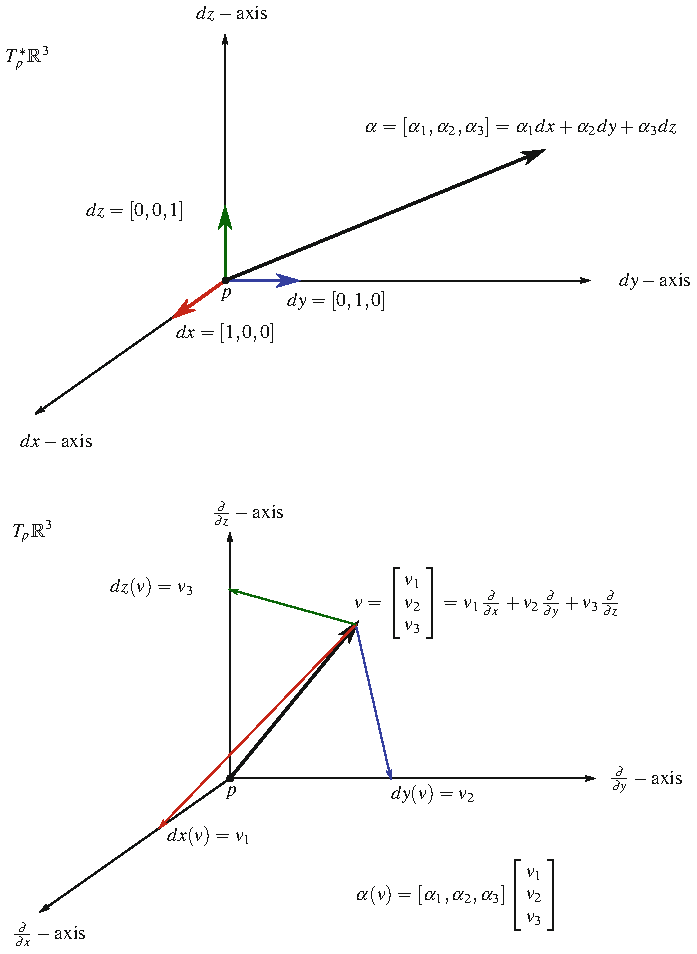
\includegraphics[width=0.826\linewidth]{images/vector/fig-3-3.pdf}
  \caption{上方，1-形式 $\alpha=\alpha_1dx+\alpha_2dy+\alpha_3dz$ 作为余切空间 $T_p^*\mathbb{R}^3$ 的元素画出. 下方，画出该 1-形式作用于向量 $v_p\in T_p\mathbb{R}^3$ 的结果}
  \label{fig:3-3}
\end{figure}

例如，由于
\[
dx_1(v_p)=dx_1\left(\begin{bmatrix}v_1\\v_2\\v_3\end{bmatrix}\right)=v_1
\]
我们可以把 $dx_1$ 看作求出向量 $v_p$ 在 $T_p\mathbb{R}^3$ 的 $\left.\frac{\partial}{\partial x_1}\right|_p$ 坐标轴上的投影. 对 $dx_2$ 与 $dx_3$ 也类似. 换言之，$dx_1$ 求出沿 $\left.\frac{\partial}{\partial x_1}\right|_p$ 坐标轴的长度. 而长度不就是一维的``体积''吗？我们希望两个 1-形式的乘积也做类似的事情，求出一个二维投影的体积. 最终这将意味着两个 1-形式的乘积将不再是 1-形式，甚至不再是线性泛函. 也就是说，它将不再是 $T_p^*\mathbb{R}^3$ 的元素，而是某种不同的东西，我们将称之为\newterm{two-form}{2-形式}{two-form}. 我们把 $\mathbb{R}^3$ 上的 2-形式空间记为 $\Lambda^2(\mathbb{R}^3)$.

在这里我们努力做到记号上非常精确，并弄清楚各个对象属于什么空间. 很容易看出混淆是如何产生的. 以图 \ref{fig:3-4} 为向导，考虑向量
\[
\begin{bmatrix}dx_1(v_p)\\dx_2(v_p)\\0\end{bmatrix}_p\in T_p\mathbb{R}^3.
\]
这个向量位于 $\mathbb{R}^3$ 在点 $p$ 处的切空间中. 换言之，它在 $T_p\mathbb{R}^3$ 中. 但这个向量也是 $v_p$ 在 $T_p\mathbb{R}^3$ 的 $\left.\frac{\partial}{\partial x_1}\right|_p\left.\frac{\partial}{\partial x_2}\right|_p$-平面上的投影. 因此我们可以把它等同于向量
\[
\binom{dx_1(v_p)}{dx_2(v_p)}_p\in\mathrm{span}\left\{\left.\frac{\partial}{\partial x_1}\right|_p,\left.\frac{\partial}{\partial x_2}\right|_p\right\}\subset T_p\mathbb{R}^3.
\]
这个向量一般被称为 $v_p$ 在 $T_p\mathbb{R}^3$ 的 $\left.\frac{\partial}{\partial x_1}\right|_p\left.\frac{\partial}{\partial x_2}\right|_p$-平面上的投影.

\begin{figure}[htbp]
  \centering
  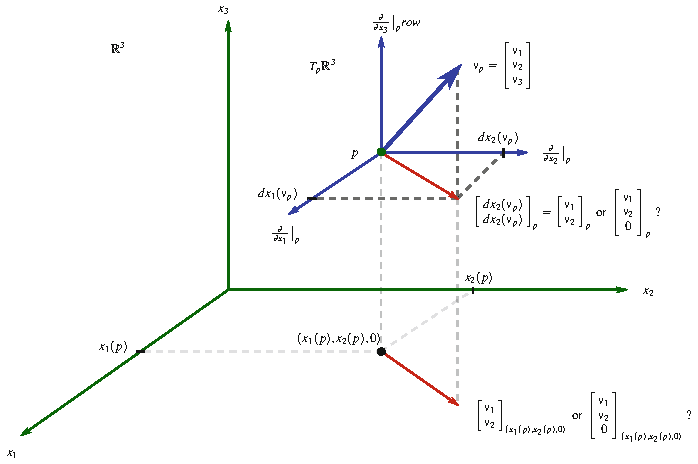
\includegraphics[width=0.960\linewidth]{images/vector/fig-3-4.pdf}
  \caption{混为一谈}
  \label{fig:3-4}
\end{figure}

再次以图 \ref{fig:3-4} 为向导来看. 注意，如果我们不够精确，就很容易把切空间中的向量
\[
\begin{bmatrix}dx_1(v_p)\\dx_2(v_p)\\0\end{bmatrix}_p\in T_p\mathbb{R}^3
\]
与 $T_p\mathbb{R}^3$ 的 $\left.\frac{\partial}{\partial x_1}\right|_p\left.\frac{\partial}{\partial x_2}\right|_p$-平面中的向量
\[
\binom{dx_1(v_p)}{dx_2(v_p)}\in T_p\mathbb{R}^3\text{ 的 }\left.\frac{\partial}{\partial x_1}\right|_p\left.\frac{\partial}{\partial x_2}\right|_p\text{-平面}
\]
与流形 $\mathbb{R}^3$ 中位于点 $p$ 处的向量
\[
\begin{bmatrix}dx_1(v_p)\\dx_2(v_p)\\0\end{bmatrix}_p\in\mathbb{R}^3
\]
甚至与流形 $\mathbb{R}^3$ 中位于点 $(x_1(p),x_2(p),0)$ 处的向量
\[
\begin{bmatrix}dx_1(v_p)\\dx_2(v_p)\\0\end{bmatrix}_{(x_1(p),x_2(p),0)}\in\mathbb{R}^3
\]
或者与 $\mathbb{R}^3$ 的 $xy$-平面中位于点 $(x_1(p),x_2(p),0)$ 处的向量
\[
\binom{dx_1(v_p)}{dx_2(v_p)}_{(x_1(p),x_2(p),0)}\in\mathbb{R}^3\text{ 的 }xy\text{-平面}
\]
混为一谈. 就 $\mathbb{R}^3$ 或 $\mathbb{R}^n$ 而言，这可能会在我们的头脑中造成混乱，但一般不会导致任何计算上的问题，这就是为什么在向量微积分中一般不做这种精确的区分. 但一般情况下我们根本不能这样做.

既然我们花了一些力气来理解各个向量所在的空间，我们就把注意力转回最初的问题：寻找两个 1-形式的乘积，使它做与 1-形式类似的事情，即求出某种体积. 正如 1-形式 $dx_1$ 输入一个向量 $v_p$ 并输出一维体积一样，我们希望两个 1-形式（比如 $dx_1$ 与 $dx_2$）的乘积输入两个向量 $v_p$ 与 $w_p$，并输出一个二维体积. 它应该给出什么体积呢？考虑图 \ref{fig:3-5}.

\begin{figure}[htbp]
  \centering
  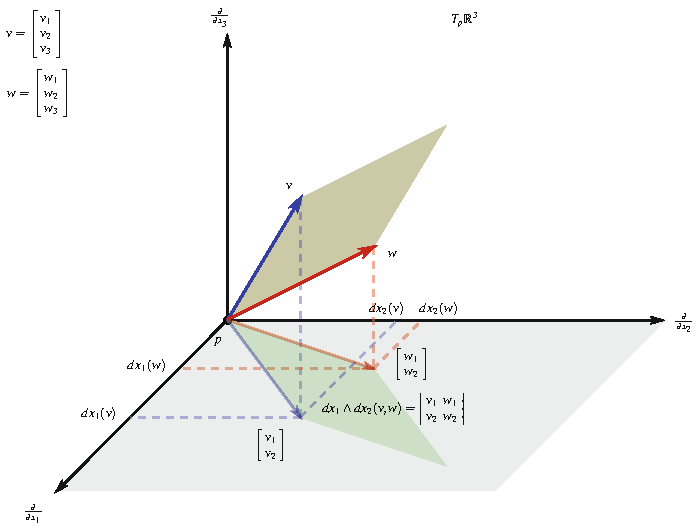
\includegraphics[width=0.960\linewidth]{images/vector/fig-3-5.pdf}
  \caption{由 $v$ 与 $w$（棕色）张成的平行六面体被投影到 $T_p\mathbb{R}^3$ 中的 $\partial x_1\partial x_2$-平面（绿色）上. 我们希望 $dx_1\wedge dx_2$ 求出这个投影区域的体积}
  \label{fig:3-5}
\end{figure}

我们已画出向量
\[
v_p=\begin{bmatrix}v_1\\v_2\\v_3\end{bmatrix}\qquad\text{与}\qquad w_p=\begin{bmatrix}w_1\\w_2\\w_3\end{bmatrix}
\]
在 $T_p\mathbb{R}^3$ 的 $\partial x_1\partial x_2$-平面上的投影. 注意我们改变了记号，把 $\left.\frac{\partial}{\partial x_i}\right|_p$ 写成了 $\partial x_i$. $v_p$ 在 $\partial x_1\partial x_2$-平面上的投影由向量
\[
\binom{dx_1(v_p)}{dx_2(v_p)}=\binom{v_1}{v_2}
\]
给出. 类似地，$w_p$ 在同一平面上的投影由
\[
\binom{dx_1(w_p)}{dx_2(w_p)}=\binom{w_1}{w_2}
\]
给出. 我们可能想要的体积中最自然的一个，是 $T_p\mathbb{R}^3$ 中 $\partial x_1\partial x_2$-平面内由这两个投影向量
\[
\binom{dx_1(v_p)}{dx_2(v_p)}\qquad\text{与}\qquad\binom{dx_1(w_p)}{dx_2(w_p)}
\]
张成的平行六面体的体积. 所以，我们希望这两个 1-形式 $dx_1$ 与 $dx_2$ 的这种``乘法''或``乘积''在输入两个向量 $v_p$ 与 $w_p$ 时能给出这个投影体积.

为了提醒我们自己这种乘法实际上不同于我们迄今为止所习惯的任何东西，我们将为它使用一种特殊的记号，称为楔号 $\wedge$，并给它起一个特别的名字，楔积. 所以，这就是我们想要的
\[
dx_1\wedge dx_2(v_p,w_p)=\text{由 }v_p\text{ 与 }w_p\text{ 在 }\partial x_1\partial x_2\text{-平面上的投影张成的平行六面体的体积}.
\]
或者，
\[
dx_1\wedge dx_2(v_p,w_p)=\text{由 }\binom{dx_1(v_p)}{dx_2(v_p)}\text{ 与 }\binom{dx_1(w_p)}{dx_2(w_p)}\text{ 张成的平行六面体的体积}.
\]
但这正是我们在第 1 章行列式那一节推导行列式定义的方式. 由向量
\[
\binom{dx_1(v_p)}{dx_2(v_p)}\qquad\text{与}\qquad\binom{dx_1(w_p)}{dx_2(w_p)}
\]
张成的平行六面体的体积，由以这些向量为列的矩阵的行列式公式给出. 因此我们可以用行列式来帮助我们定义楔积，
\[
dx_1\wedge dx_2(v_p,w_p)\equiv
\begin{vmatrix}
dx_1(v_p) & dx_1(w_p)\\
dx_2(v_p) & dx_2(w_p)
\end{vmatrix}.
\]
总之，两个 1-形式的楔积是用相应的向量投影的行列式来定义的. 所以我们看到，体积、行列式与投影（通过 1-形式）在楔积的定义中全部混合在一起并密切相关. 更一般地，两个 1-形式 $dx_i$ 与 $dx_j$ 的楔积定义为
\[
\text{两个 1-形式的楔积：}\qquad
dx_i\wedge dx_j(v_p,w_p)\equiv
\begin{vmatrix}
dx_i(v_p) & dx_i(w_p)\\
dx_j(v_p) & dx_j(w_p)
\end{vmatrix}.
\]

继续停留在流形 $\mathbb{R}^3$ 上，让我们试着对正在发生的事情获得一幅更好的图像. 回头参考图 \ref{fig:3-5}，其中两个向量 $v$ 与 $w$ 画在某个任意点 $p$ 处的切空间 $T_p\mathbb{R}^3$ 中. （此后记号中省略点 $p$.）$v$ 与 $w$ 在 $\partial x_1\partial x_2$-平面上的投影由
\[
\binom{dx_1(v_p)}{dx_2(v_p)}=\binom{v_1}{v_2}\qquad\text{与}\qquad\binom{dx_1(w_p)}{dx_2(w_p)}=\binom{w_1}{w_2}
\]
给出. 由这些投影张成的平行六面体的面积由 $dx_1\wedge dx_2(v,w)$ 给出. 作为例子，假设
\[
v=\begin{bmatrix}1\\2\\3\end{bmatrix}\qquad\text{与}\qquad w=\begin{bmatrix}4\\5\\6\end{bmatrix}.
\]
首先我们求 $dx_1\wedge dx_2(v,w)$：
\[
dx_1\wedge dx_2\left(\begin{bmatrix}1\\2\\3\end{bmatrix},\begin{bmatrix}4\\5\\6\end{bmatrix}\right)
=\begin{vmatrix}1&4\\2&5\end{vmatrix}=(1)(5)-(4)(2)=-3.
\]
注意我们得到的面积是 $-3$. 这不应该令人惊讶，因为我们知道面积实际上是有符号的. 如果我们改求 $dx_2\wedge dx_1(v,w)$：
\[
dx_2\wedge dx_1\left(\begin{bmatrix}1\\2\\3\end{bmatrix},\begin{bmatrix}4\\5\\6\end{bmatrix}\right)
=\begin{vmatrix}2&5\\1&4\end{vmatrix}=(2)(4)-(5)(1)=3
\]
我们就得到面积 3. 有一点需要提醒，当计算 $dx_1\wedge dx_2$ 时，我们的投影向量是
\[
\binom{dx_1(v_p)}{dx_2(v_p)}=\binom{1}{2}\qquad\text{与}\qquad\binom{dx_1(w_p)}{dx_2(w_p)}=\binom{4}{5}
\]
而当计算 $dx_2\wedge dx_1$ 时，我们的投影向量是
\[
\binom{dx_2(v_p)}{dx_1(v_p)}=\binom{2}{1}\qquad\text{与}\qquad\binom{dx_2(w_p)}{dx_1(w_p)}=\binom{5}{4}
\]
它们看起来可能是不同的向量. 然而它们并不是不同的向量. 我们只是把向量的分量写成不同的顺序，仅此而已. 我们不是像通常那样先写 $x_1$ 分量，而是先写了 $x_2$ 分量.

在图 \ref{fig:3-6} 中，同样的两个向量 $v$ 与 $w$ 画在某个任意点 $p$ 处的同一个切空间 $T_p\mathbb{R}^3$ 中. （同样，此后记号中省略点 $p$.）$v$ 与 $w$ 在 $\partial x_2\partial x_3$-平面上的投影由
\[
\binom{dx_2(v_p)}{dx_3(v_p)}=\binom{v_2}{v_3}\qquad\text{与}\qquad\binom{dx_2(w_p)}{dx_3(w_p)}=\binom{w_2}{w_3}
\]
给出. 由这些投影张成的平行六面体的面积由 $dx_2\wedge dx_3(v,w)$ 给出. 继续使用同一个例子，我们求 $dx_2\wedge dx_3(v,w)$：
\[
dx_2\wedge dx_3\left(\begin{bmatrix}1\\2\\3\end{bmatrix},\begin{bmatrix}4\\5\\6\end{bmatrix}\right)
=\begin{vmatrix}2&5\\3&6\end{vmatrix}=(2)(6)-(3)(5)=-3.
\]
而 $dx_3\wedge dx_2(v,w)$ 给出
\[
dx_3\wedge dx_2\left(\begin{bmatrix}1\\2\\3\end{bmatrix},\begin{bmatrix}4\\5\\6\end{bmatrix}\right)
=\begin{vmatrix}3&6\\2&5\end{vmatrix}=(3)(5)-(6)(2)=3.
\]

\begin{figure}[htbp]
  \centering
  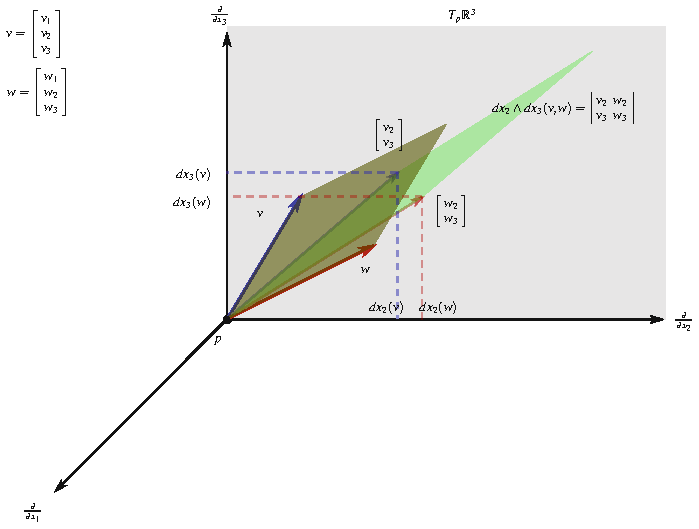
\includegraphics[width=0.960\linewidth]{images/vector/fig-3-6.pdf}
  \caption{由 $v$ 与 $w$（棕色）张成的平行六面体被投影到 $T_p\mathbb{R}^3$ 中的 $\partial x_2\partial x_3$-平面（绿色）上. 当输入向量 $v$ 与 $w$ 时，楔积 $dx_2\wedge dx_3$ 将求出该投影区域的体积}
  \label{fig:3-6}
\end{figure}

再次地，同样的两个向量 $v$ 与 $w$ 画在同一个切空间 $T_p\mathbb{R}^3$ 中，$v$ 与 $w$ 在 $\partial x_1\partial x_3$-平面上的投影由
\[
\binom{dx_1(v_p)}{dx_3(v_p)}=\binom{v_1}{v_3}\qquad\text{与}\qquad\binom{dx_1(w_p)}{dx_3(w_p)}=\binom{w_1}{w_3}
\]
给出. 这如图 \ref{fig:3-7} 所示. 由这些投影张成的平行六面体的面积由 $dx_1\wedge dx_3(v,w)$ 给出. 使用同一个例子，我们求 $dx_1\wedge dx_3(v,w)$：
\[
dx_1\wedge dx_3\left(\begin{bmatrix}1\\2\\3\end{bmatrix},\begin{bmatrix}4\\5\\6\end{bmatrix}\right)
=\begin{vmatrix}1&4\\3&6\end{vmatrix}=(1)(6)-(3)(4)=-6.
\]
而 $dx_3\wedge dx_1(v,w)$ 给出
\[
dx_3\wedge dx_1\left(\begin{bmatrix}1\\2\\3\end{bmatrix},\begin{bmatrix}4\\5\\6\end{bmatrix}\right)
=\begin{vmatrix}3&6\\1&4\end{vmatrix}=(3)(4)-(1)(6)=6.
\]

\begin{figure}[htbp]
  \centering
  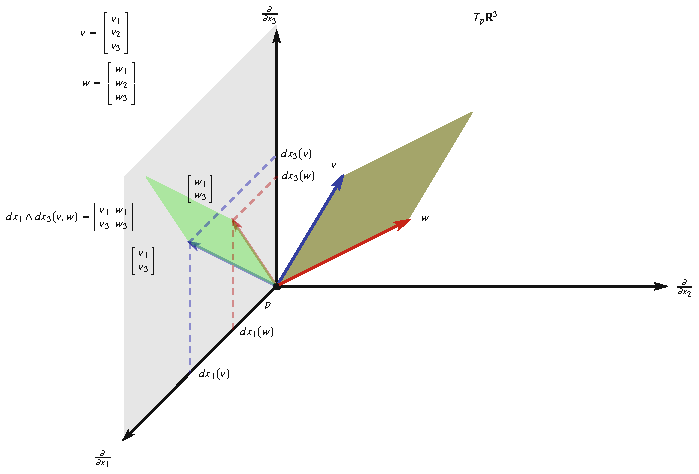
\includegraphics[width=0.960\linewidth]{images/vector/fig-3-7.pdf}
  \caption{由 $v$ 与 $w$（棕色）张成的平行六面体被投影到 $T_p\mathbb{R}^3$ 中的 $\partial x_1\partial x_3$-平面（绿色）上. 当输入向量 $v$ 与 $w$ 时，楔积 $dx_1\wedge dx_3$ 将求出该投影区域的体积}
  \label{fig:3-7}
\end{figure}

基于这些例子，看起来 $dx_i\wedge dx_j=-dx_j\wedge dx_i$. 利用上面给出的楔积定义，容易看出确实有 $dx_i\wedge dx_j=-dx_j\wedge dx_i$. 这个性质称为\newterm{skew-symmetry}{反对称性}{skew symmetry}，它由行列式的性质推出. 回忆一下，如果你交换行列式中的两行，行列式的符号就会改变. 这里发生的事情本质上就是如此. 这意味着两个 1-形式``相乘''（通过楔积）的顺序是有关系的. 如果我们交换顺序，答案就会改变一个符号.

继续使用同样的向量 $v=\begin{bmatrix}1\\2\\3\end{bmatrix}$ 与 $w=\begin{bmatrix}4\\5\\6\end{bmatrix}$，让我们求 $dx_1\wedge dx_1(v_p,w_p)$：
\[
dx_1\wedge dx_1\left(\begin{bmatrix}1\\2\\3\end{bmatrix},\begin{bmatrix}4\\5\\6\end{bmatrix}\right)
=\begin{vmatrix}1&4\\1&4\end{vmatrix}=(1)(4)-(4)(1)=0.
\]
类似地，我们有 $dx_2\wedge dx_2(v,w)=0$ 与 $dx_3\wedge dx_3(v,w)=0$. 这不应该太令人惊讶，因为一般来说我们会有
\[
dx_i\wedge dx_i(v,w)=
\begin{vmatrix}
dx_i(v) & dx_i(w)\\
dx_i(v) & dx_i(w)
\end{vmatrix}
=dx_i(v)\cdot dx_i(w)-dx_i(v)\cdot dx_i(w)=0.
\]
另一种看待这一点的方式是注意到，由 $dx_i\wedge dx_j=-dx_j\wedge dx_i$ 可以推出 $dx_i\wedge dx_i=-dx_i\wedge dx_i$，这只有当 $dx_i\wedge dx_i=0$ 时才可能发生. 遗憾的是，没有任何一幅精确的图能展示这里发生的事情. 最好就是认识到，由投影向量张成的平行六面体是退化的，因此面积为零.

所以，给定 $T_p\mathbb{R}^3$ 中的两个向量 $v_p$ 与 $w_p$，我们现在已经考虑了所有可能的两个 1-形式的楔积. 我们考虑了
\[
dx_1\wedge dx_2,\qquad dx_2\wedge dx_3,\qquad dx_1\wedge dx_3.
\]
我们还发现
\[
dx_1\wedge dx_2=-dx_2\wedge dx_1,\qquad
dx_2\wedge dx_3=-dx_3\wedge dx_2,\qquad
dx_1\wedge dx_3=-dx_3\wedge dx_1,
\]
所以一旦我们知道左边对两个向量的作用，就自动知道右边对同样这两个向量的作用. 最后，我们还发现
\[
dx_1\wedge dx_1=0,\qquad dx_2\wedge dx_2=0,\qquad dx_3\wedge dx_3=0.
\]
全部情况就是这些. 楔积 $dx_1\wedge dx_2$、$dx_2\wedge dx_3$ 与 $dx_1\wedge dx_3$ 都称为 2-形式. 事实上，每一个 2-形式都可以写成这三个 2-形式的线性组合. 例如，对任意 $a,b,c\in\mathbb{R}$，$a\,dx_1\wedge dx_2+b\,dx_2\wedge dx_3+c\,dx_1\wedge dx_3$ 都是 2-形式. 出于这个原因，2-形式 $dx_1\wedge dx_2$、$dx_2\wedge dx_3$ 与 $dx_1\wedge dx_3$ 被称为 $\mathbb{R}^3$ 上 2-形式空间的基，该空间记为 $\Lambda^2(\mathbb{R}^3)$. 实际上，有一个习惯或约定，用 2-形式 $dx_1\wedge dx_2$、$dx_2\wedge dx_3$ 与 $dx_3\wedge dx_1$ 作为 $\Lambda^2(\mathbb{R}^3)$ 的基. 我们只是把 $dx_1\wedge dx_3$ 替换成了 $dx_3\wedge dx_1$. 这样做的原因是为了在写下基时保持一种``循环次序''，而这只能在三维中做到. 但关于这一点，下一节还会详细讨论.

到目前为止我们一直在 $\mathbb{R}^3$ 上工作，因为它容易画出图像，也容易看清我们所说的投影是什么意思. 现在让我们退后一步，如图 \ref{fig:3-8} 所示，花一点时间思考 $\mathbb{R}^2$. 向量 $v_p=\binom{v_1}{v_2}$ 在 $T_p\mathbb{R}^2$ 的一维子空间 $\partial x_1$ 上的投影由向量 $[dx_1(v_p)]=[v_1]$ 给出，$v_p$ 在子空间 $\partial x_2$ 上的投影由向量 $[dx_2(v_p)]=[v_2]$ 给出，如图所示.

\begin{figure}[htbp]
  \centering
  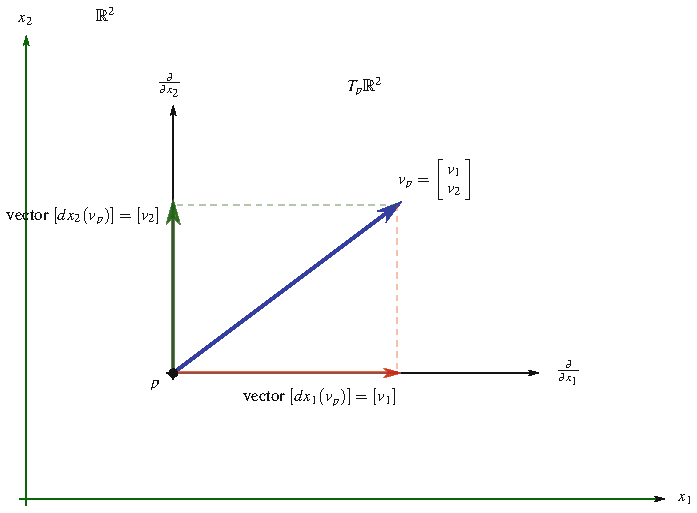
\includegraphics[width=0.826\linewidth]{images/vector/fig-3-8.pdf}
  \caption{流形 $\mathbb{R}^2$ 及其上叠加的切空间 $T_p\mathbb{R}^2$. 向量 $v_p$ 是切空间 $T_p\mathbb{R}^2$ 的一个元素}
  \label{fig:3-8}
\end{figure}

但现在考虑图 \ref{fig:3-9}. 它与图 \ref{fig:3-8} 类似，只是现在有两个向量 $v_p$ 与 $w_p$ 位于 $T_p\mathbb{R}^2$ 中，它们张成一个平行六面体. 在这里 $dx_1\wedge dx_2(v_p,w_p)$ 表示什么呢？在这种情况下 $v_p$ 与 $w_p$ 被投影到什么空间呢？我们有
\[
dx_1\wedge dx_2(v_p,w_p)
=\begin{vmatrix}
dx_1(v_p) & dx_1(w_p)\\
dx_2(v_p) & dx_2(w_p)
\end{vmatrix}
=\begin{vmatrix}
v_1 & w_1\\
v_2 & w_2
\end{vmatrix}
=v_1w_2-w_1v_2
\]
这正是由
\[
\binom{dx_1(v_p)}{dx_2(v_p)}=\binom{v_1}{v_2}=v_p
\qquad\text{与}\qquad
\binom{dx_1(w_p)}{dx_2(w_p)}=\binom{w_1}{w_2}=w_p
\]
张成的平行六面体的面积，所以 $v_p$ 与 $w_p$ 被``投影''到的空间是整个空间 $T_p\mathbb{R}^2$.

\begin{figure}[htbp]
  \centering
  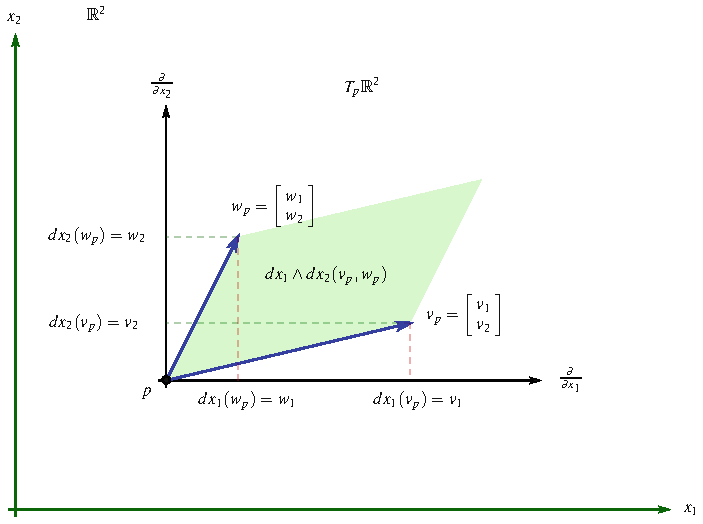
\includegraphics[width=0.833\linewidth]{images/vector/fig-3-9.pdf}
  \caption{流形 $\mathbb{R}^2$ 及其上叠加的切空间 $T_p\mathbb{R}^2$. 由 $v_p$ 与 $w_p$ 张成的平行六面体已画出. 但当 $dx_1\wedge dx_2$ 作用于向量 $v_p$ 与 $w_p$ 时，它会被投影到什么空间呢？它被投影到它已经所在的空间，即 $T_p\mathbb{R}^2$}
  \label{fig:3-9}
\end{figure}

\begin{question}\label{q:3-1}
求 $dx_2\wedge dx_1(v_p,w_p)$. 它与 $dx_1\wedge dx_2(v_p,w_p)$ 有何关系？$\Lambda_p^2(\mathbb{R}^2)$ 的基是什么？$\Lambda_p^2(\mathbb{R}^2)$ 的一般元素长什么样？
\end{question}

\begin{question}\label{q:3-2}
目前我们继续停留在 $\mathbb{R}^2$ 的例子中.
\begin{enumerate}
  \item[(a)] 考虑 $dx_1\wedge dx_2\wedge dx_1$. 你认为它需要几个向量作为输入？
  \item[(b)] 在二维空间中，由三个向量张成的平行六面体的三维体积是多少？
  \item[(c)] 设 $u=\binom{u_1}{u_2}$、$v=\binom{v_1}{v_2}$、$s=\binom{w_1}{w_2}$，并设
  \[
  dx_1\wedge dx_2\wedge dx_1(u,v,w)\equiv
  \begin{vmatrix}
  dx_1(u) & dx_1(v) & dx_1(w)\\
  dx_2(u) & dx_2(v) & dx_2(w)\\
  dx_1(u) & dx_1(v) & dx_1(w)
  \end{vmatrix}.
  \]
  解释为什么它总是零.
  \item[(d)] 基于此，你认为空间 $\Lambda_p^3(\mathbb{R}^2)$ 会是什么？
  \item[(e)] 基于此，你认为当 $n>3$ 时空间 $\Lambda_p^n(\mathbb{R}^2)$ 会是什么？
\end{enumerate}
\end{question}

我们把三个 1-形式的楔积定义如下：
\[
\text{三个 1-形式的楔积：}\qquad
dx_i\wedge dx_j\wedge dx_k(u,v,w)\equiv
\begin{vmatrix}
dx_i(u) & dx_i(v) & dx_i(w)\\
dx_j(u) & dx_j(v) & dx_j(w)\\
dx_k(u) & dx_k(v) & dx_k(w)
\end{vmatrix}.
\]
我们将三个 1-形式 $dx_i\wedge dx_j\wedge dx_k$ 的楔积称为\newterm{three-form}{3-形式}{three-form}. 这个 3-形式 $dx_i\wedge dx_j\wedge dx_k$ 求出什么呢？假设我们在流形 $\mathbb{R}^n$ 上. 给定点 $p$ 处的向量 $u,v,w$，我们首先求出这些向量在 $T_p\mathbb{R}^n$ 的 $\partial x_i\partial x_j\partial x_k$-子空间上的投影. 这些投影由向量
\[
\begin{bmatrix}dx_i(u)\\dx_j(u)\\dx_k(u)\end{bmatrix},\qquad
\begin{bmatrix}dx_i(v)\\dx_j(v)\\dx_k(v)\end{bmatrix},\qquad
\begin{bmatrix}dx_i(w)\\dx_j(w)\\dx_k(w)\end{bmatrix}
\]
给出.

接下来，我们利用行列式求出由这些投影向量张成的平行六面体的体积. 回到 $\mathbb{R}^3$，我们考虑 3-形式 $dx_1\wedge dx_2\wedge dx_3$. 3-形式 $dx_1\wedge dx_2\wedge dx_3$ 投影到 $T_p\mathbb{R}^3$ 的什么子空间上呢？3-形式 $dx_1\wedge dx_2\wedge dx_3$ 投影到整个空间 $T_p\mathbb{R}^3$ 上. 因此 3-形式 $dx_1\wedge dx_2\wedge dx_3$ 只是求出由三个输入向量张成的平行六面体的体积，见图 \ref{fig:3-10}.

\begin{figure}[htbp]
  \centering
  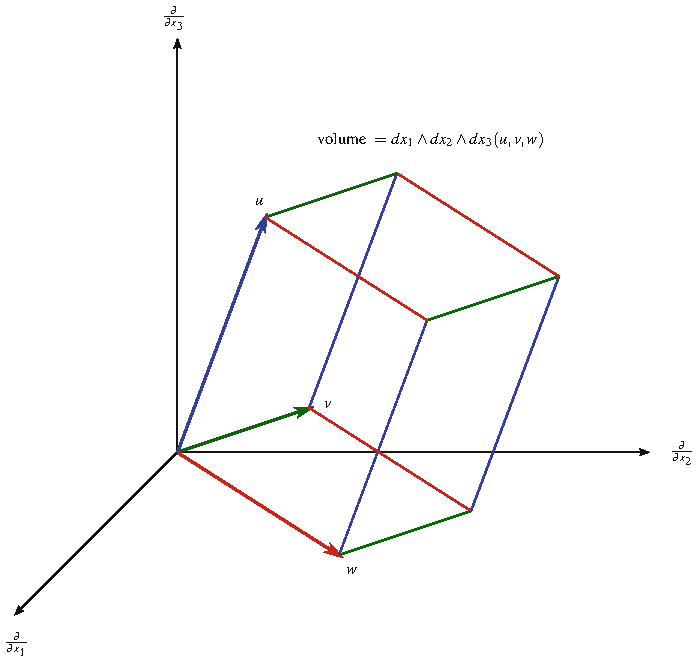
\includegraphics[width=0.829\linewidth]{images/vector/fig-3-10.pdf}
  \caption{切空间 $T_p\mathbb{R}^3$ 及由 $u$、$v$、$w$ 张成的平行六面体. 3-形式 $dx_1\wedge dx_2\wedge dx_3$（这里写为 $dx\wedge dy\wedge dz$）只是求出该平行六面体的体积}
  \label{fig:3-10}
\end{figure}

\begin{question}\label{q:3-3}
考虑流形 $\mathbb{R}^3$ 与 3-形式 $dx_1\wedge dx_2\wedge dx_3$.
\begin{enumerate}
  \item[(a)] $dx_1\wedge dx_2\wedge dx_3$ 与 $dx_2\wedge dx_1\wedge dx_3$ 有何关系？与 $dx_2\wedge dx_3\wedge dx_1$ 呢？或者 $dx_3\wedge dx_2\wedge dx_1$ 呢？你注意到什么规律了吗？
  \item[(b)] $\Lambda_p^3(\mathbb{R}^3)$ 的基是什么？
  \item[(c)] 你认为 $dx_1\wedge dx_2\wedge dx_3\wedge dx_1(u,v,w,x)$ 会如何定义？你认为它会是什么？为什么？（这里的输入 $x$ 表示第四个向量.）
  \item[(d)] 当 $n\geq4$ 时，$\Lambda_p^n(\mathbb{R}^3)$ 是什么？
\end{enumerate}
\end{question}

一般地，设 $v_1,v_2,\ldots,v_n$ 表示向量，我们把 $n$ 个 1-形式的楔积定义如下：
\[
\text{楔积（n 个 1-形式）：}\\[2mm]
dx_{i_1}\wedge dx_{i_2}\wedge\cdots\wedge dx_{i_n}(v_1,v_2,\ldots,v_n)\equiv
{\setlength{\arraycolsep}{0.5pt}\begin{vmatrix}
dx_{i_1}(v_1) & dx_{i_1}(v_2) & \cdots & dx_{i_1}(v_n)\\
dx_{i_2}(v_1) & dx_{i_2}(v_2) & \cdots & dx_{i_2}(v_n)\\
\vdots & \vdots & \ddots & \vdots\\
dx_{i_n}(v_1) & dx_{i_n}(v_2) & \cdots & dx_{i_n}(v_n)
\end{vmatrix}}.
\]
注意，如果任意两个 1-形式相同，即对某个 $j\neq k$ 有 $i_j=i_k$，那么我们就有两行相同，这给出值零.

为了结束本节，我们将考虑流形 $\mathbb{R}$ 上的 1-形式 $dx$、流形 $\mathbb{R}^2$ 上的 2-形式 $dx_1\wedge dx_2$、流形 $\mathbb{R}^3$ 上的 3-形式 $dx_1\wedge dx_2\wedge dx_3$，以及流形 $\mathbb{R}^n$ 上的 n-形式 $dx_1\wedge dx_2\wedge\cdots\wedge dx_n$. 这些是非常特殊的微分形式，通常被称为\newterm{volume-form}{体积形式}{volume form}，不过在二维情形中，2-形式 $dx_1\wedge dx_2$ 也常被称为\newterm{area-form}{面积形式}{area form}. 学完本节之后，这个术语背后的原因是相当明显的. 1-形式 $dx$ 求出 $\mathbb{R}$ 上向量的一维体积，即长度. 类似地，2-形式 $dx_1\wedge dx_2$（也写为 $dx\wedge dy$）求出 $\mathbb{R}^2$ 上平行六面体的二维体积，即面积（图 \ref{fig:3-9}）；3-形式 $dx_1\wedge dx_2\wedge dx_3$（也写为 $dx\wedge dy\wedge dz$）求出 $\mathbb{R}^3$ 上平行六面体的三维体积（图 \ref{fig:3-10}）；显然 n-形式 $dx_1\wedge dx_2\wedge\cdots\wedge dx_n$ 求出 $\mathbb{R}^n$ 上平行六面体的 n 维体积. 严格地说，被求体积的平行六面体实际上位于某个切空间中而不是流形中，但对于欧几里得空间，我们实际上也可以想象平行六面体位于流形本身中，所以我们就不在这个问题上过分纠缠了. 当我们讲到形式的积分时，这些体积形式将扮演至关重要的角色.

\begin{question}\label{q:3-4}
考虑 n-形式 $dx_{i_1}\wedge dx_{i_2}\wedge\cdots\wedge dx_{i_n}$. 如果某个 1-形式 $dx_{i_j}=dx_{i_k}$（其中 $i_j\neq i_k$）会怎样？如果某个向量 $v_j=v_k$（其中 $j\neq k$）会怎样？
\end{question}

\begin{question}\label{q:3-5}
证明：若 $i_j\neq i_k$，则交换 $dx_{i_j}$ 与 $dx_{i_k}$ 会使楔积改变符号.
\end{question}

\section{一般的 2-形式与 3-形式}

2-形式是由两个 1-形式楔乘在一起构成的. 正如我们用 $T_p^*\mathbb{R}^3$ 表示点 $p$ 处的余切空间（它是点 $p$ 处的 1-形式空间）一样，我们把点 $p$ 处的 2-形式空间记为 $\Lambda_p^2(\mathbb{R}^3)$. 与此约定一致，你偶尔会看到 $T_p^*\mathbb{R}^3$ 被写为 $\Lambda_p^1(\mathbb{R}^3)$. 正如我们已经提到的，空间 $\Lambda_p^2(\mathbb{R}^3)$ 的基由
\[
\{dx_1\wedge dx_2,\;dx_2\wedge dx_3,\;dx_3\wedge dx_1\}
\]
给出. 为什么列表中的最后一个元素写成 $dx_3\wedge dx_1$ 而不是 $dx_1\wedge dx_3$？这纯粹是基于希望循环地书写指标（index）的约定问题. 这些基元素 $dx_1\wedge dx_2$、$dx_2\wedge dx_3$、$dx_3\wedge dx_1$ 中的每一个都求出两个向量在 $T_p\mathbb{R}^3$ 的适当平面上的投影所张成的平行六面体的有向面积，如图 \ref{fig:3-11} 所示.

\begin{figure}[htbp]
  \centering
  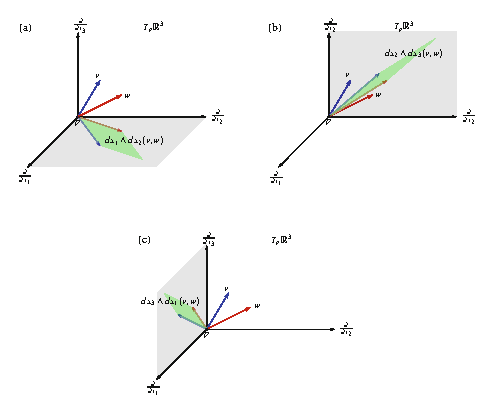
\includegraphics[width=0.880\linewidth]{images/vector/fig-3-11.pdf}
  \caption{$\Lambda^2(\mathbb{R}^3)$ 的基元素的几何作用：把 $v$ 与 $w$ 投影到 $T_p\mathbb{R}^3$ 中适当的平面上，然后求出由投影张成的平行六面体的有向面积，该面积以绿色显示. (a) $dx_1\wedge dx_2$ 的作用. (b) $dx_2\wedge dx_3$ 的作用. (c) $dx_3\wedge dx_1$ 的作用}
  \label{fig:3-11}
\end{figure}

类似地，不难看出空间 $\Lambda_p^2(\mathbb{R}^2)$ 的基由
\[
\{dx_1\wedge dx_2\}
\]
给出，而空间 $\Lambda_p^2(\mathbb{R}^4)$ 的基由
\[
\{dx_1\wedge dx_2,\;dx_1\wedge dx_3,\;dx_1\wedge dx_4,\;dx_2\wedge dx_3,\;dx_2\wedge dx_4,\;dx_3\wedge dx_4\}
\]
给出，等等. $\Lambda_p^2(\mathbb{R}^n)$ 的基含有 $\frac{n(n-1)}{2}$ 个元素.

\begin{question}\label{q:3-6}
解释为什么 $\{dx_1\wedge dx_2\}$ 是 $\Lambda_p^2(\mathbb{R}^2)$ 的基，为什么 $\{dx_1\wedge dx_2,dx_1\wedge dx_3,dx_1\wedge dx_4,dx_2\wedge dx_3,dx_2\wedge dx_4,dx_3\wedge dx_4\}$ 是 $\Lambda_p^2(\mathbb{R}^4)$ 的基.
\end{question}

\begin{question}\label{q:3-7}
解释为什么 $\Lambda_p^2(\mathbb{R}^n)$ 的基含有 $\frac{n(n-1)}{2}$ 个元素.
\end{question}

到目前为止，我们只看过 2-形式的基元素. 但空间 $\Lambda_p^2(\mathbb{R}^2)$、$\Lambda_p^2(\mathbb{R}^3)$、$\Lambda_p^2(\mathbb{R}^4)$ 或 $\Lambda_p^2(\mathbb{R}^n)$ 中的其他元素又如何呢？它们长什么样、做什么？目前我们集中讨论空间 $\Lambda_p^2(\mathbb{R}^3)$，因此将采用记号 $x,y,z$ 而不是 $x_1,x_2,x_3$.

考虑 2-形式 $5dx\wedge dy$ 作用于某个 $p$ 的两个向量 $v_p$ 与 $w_p$. 因子 5 做什么？$dx\wedge dy(v_p,w_p)$ 给出由 $v_p$ 与 $w_p$ 在 $\partial x\partial y$-平面上的投影张成的平行六面体的面积. 数字五把面积乘以五，从而缩放这个面积. 因此基元素 $dx\wedge dy$、$dy\wedge dz$、$dz\wedge dx$ 前面的数值因子是缩放因子.

图 \ref{fig:3-12} 试图展示形如 $dx\wedge dy+dy\wedge dz$ 的 2-形式对 $T_p\mathbb{R}^3$ 中两个向量 $v$ 与 $w$ 的作用. 先求出 $v$ 与 $w$ 在 $\partial x\partial y$-平面上的投影
\[
\binom{dx(v)}{dy(v)}\qquad\text{与}\qquad\binom{dx(w)}{dy(w)}
\]
并画出由这两个投影向量在 $\partial x\partial y$-平面中形成的平行六面体. $dx\wedge dy(v,w)$ 求出这个平行六面体的有向面积. 然后求出 $v$ 与 $w$ 在 $\partial y\partial z$-平面上的投影
\[
\binom{dy(v)}{dz(v)}\qquad\text{与}\qquad\binom{dy(w)}{dz(w)}
\]
并同样画出由这两个投影向量在 $\partial y\partial z$-平面中形成的平行六面体. $dy\wedge dz(v,w)$ 求出这个平行六面体的有向面积. 2-形式 $dx\wedge dy+dy\wedge dz$ 把这两个有向面积相加：
\[
\bigl(dx\wedge dy+dy\wedge dz\bigr)(v,w)=dx\wedge dy(v,w)+dy\wedge dz(v,w).
\]
形如 $adx\wedge dy+bdy\wedge dz$（其中 $a,b\in\mathbb{R}$）的 2-形式在相加之前先把平行六面体面积乘以因子 $a$ 与 $b$：
\[
\bigl(adx\wedge dy+bdy\wedge dz\bigr)(v,w)=adx\wedge dy(v,w)+bdy\wedge dz(v,w).
\]

\begin{figure}[htbp]
  \centering
  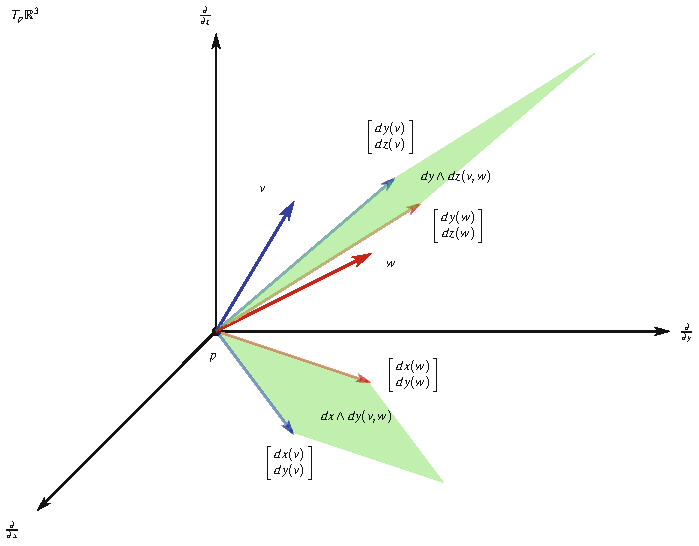
\includegraphics[width=0.944\linewidth]{images/vector/fig-3-12.pdf}
  \caption{2-形式 $dx\wedge dy+dy\wedge dz$ 对两个向量 $v$ 与 $w$ 的作用. 2-形式 $dx\wedge dy+dy\wedge dz$ 求出两个投影平行六面体的面积之和}
  \label{fig:3-12}
\end{figure}

图 \ref{fig:3-13} 表明，2-形式 $dy\wedge dz+dz\wedge dx$ 对 $T_p\mathbb{R}^3$ 中两个向量 $v$ 与 $w$ 的作用本质上是类似的. 先求出 $v$ 与 $w$ 在 $\partial y\partial z$-平面上的投影
\[
\binom{dy(v)}{dz(v)}\qquad\text{与}\qquad\binom{dy(w)}{dz(w)}
\]
并画出由这两个投影向量在 $\partial y\partial z$-平面中形成的平行六面体. $dy\wedge dz(v,w)$ 求出这个平行六面体的有向面积. 然后求出 $v$ 与 $w$ 在 $\partial x\partial z$-平面上的投影
\[
\binom{dx(v)}{dz(v)}\qquad\text{与}\qquad\binom{dx(w)}{dz(w)}
\]
并同样画出由这两个投影向量在 $\partial x\partial z$-平面中形成的平行六面体. $dz\wedge dx(v,w)$ 求出这个平行六面体的有向面积. 2-形式 $dy\wedge dz+dz\wedge dx$ 把这两个有向面积相加：
\[
\bigl(dy\wedge dz+dz\wedge dx\bigr)(v,w)=dy\wedge dz(v,w)+dz\wedge dx(v,w).
\]
形如 $ady\wedge dz+bdz\wedge dx$（其中 $a,b\in\mathbb{R}$）的 2-形式在相加之前先把平行六面体面积乘以因子 $a$ 与 $b$：
\[
\bigl(ady\wedge dz+bdz\wedge dx\bigr)(v,w)=ady\wedge dz(v,w)+bdz\wedge dx(v,w).
\]

\begin{figure}[htbp]
  \centering
  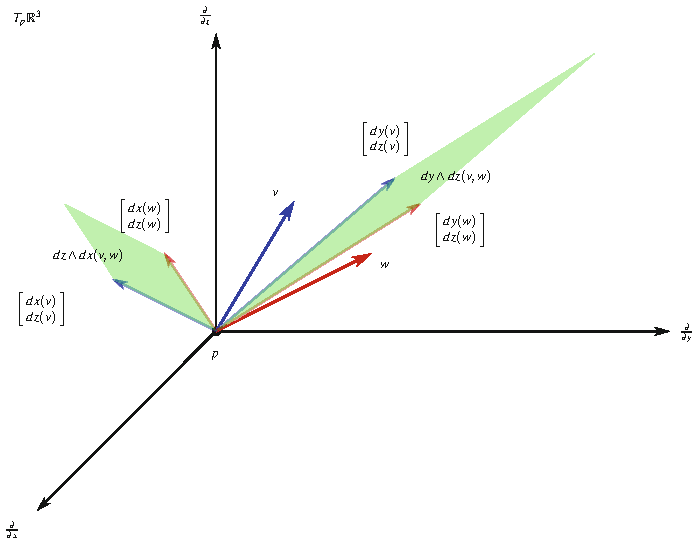
\includegraphics[width=0.944\linewidth]{images/vector/fig-3-13.pdf}
  \caption{2-形式 $dy\wedge dz+dz\wedge dx$ 对两个向量 $v$ 与 $w$ 的作用. 2-形式 $dy\wedge dz+dz\wedge dx$ 求出两个投影平行六面体的面积之和}
  \label{fig:3-13}
\end{figure}

不再重复所有细节，2-形式 $dx\wedge dy+dz\wedge dx$ 与 $adx\wedge dy+bdz\wedge dx$ 作用于两个向量 $v,w\in T_p\mathbb{R}^3$ 时的行为是类似的，见图 \ref{fig:3-14}.

\begin{figure}[htbp]
  \centering
  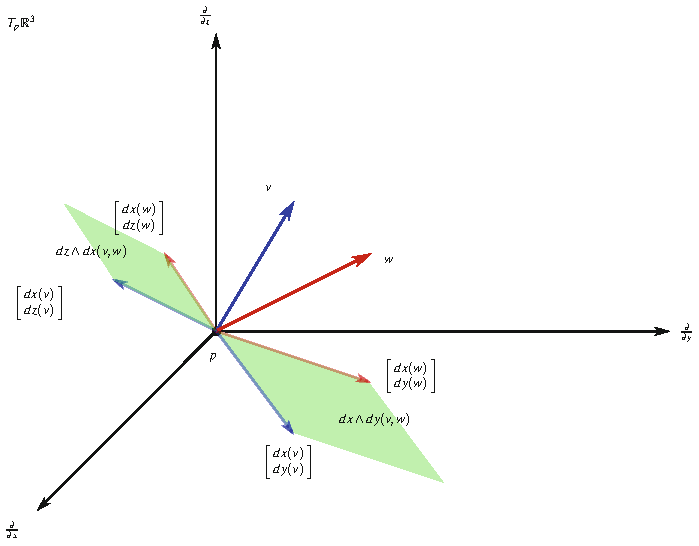
\includegraphics[width=0.944\linewidth]{images/vector/fig-3-14.pdf}
  \caption{2-形式 $dx\wedge dy+dz\wedge dx$ 对两个向量 $v$ 与 $w$ 的作用. 2-形式 $dx\wedge dy+dz\wedge dx$ 求出两个投影平行六面体的面积之和}
  \label{fig:3-14}
\end{figure}

最后，我们考虑形如 $dx\wedge dy+dy\wedge dz+dz\wedge dx$ 的 2-形式. 这种 2-形式作用于两个向量 $v,w\in T_p\mathbb{R}^3$ 的方式与你预期完全一致，如图 \ref{fig:3-15} 所示. 首先求出在 $T_p\mathbb{R}^3$ 各不同平面上的投影. 然后画出由这些投影向量形成的平行六面体. $dx\wedge dy(v,w)$ 求出 $\partial x\partial y$-平面中平行六面体的有向体积，$dy\wedge dz(v,w)$ 求出 $\partial y\partial z$-平面中平行六面体的有向体积，$dz\wedge dx(v,w)$ 求出 $\partial x\partial z$-平面中平行六面体的有向体积. 然后把这些有向体积相加：
\[
\bigl(dx\wedge dy+dy\wedge dz+dz\wedge dx\bigr)(v,w)=dx\wedge dy(v,w)+dy\wedge dz(v,w)+dz\wedge dx(v,w).
\]
形如 $adx\wedge dy+bdy\wedge dz+cdz\wedge dx$（其中 $a,b,c\in\mathbb{R}$）的 2-形式的工作方式类似，只是各个有向体积在相加之前分别被因子 $a,b,c$ 缩放.

\begin{figure}[htbp]
  \centering
  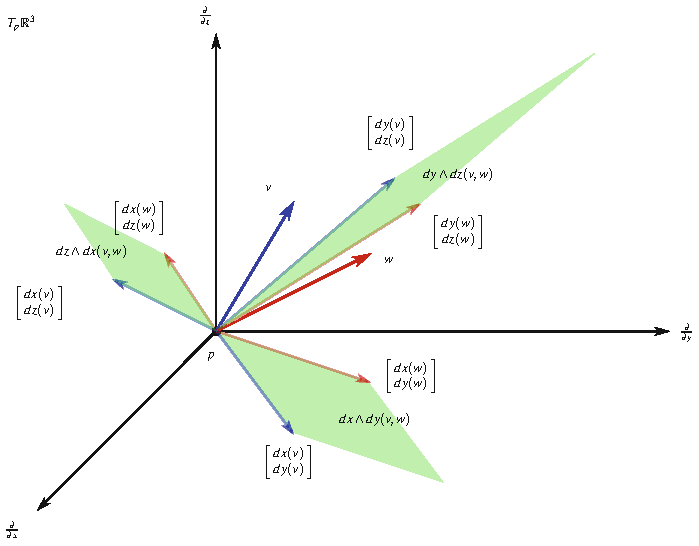
\includegraphics[width=0.944\linewidth]{images/vector/fig-3-15.pdf}
  \caption{2-形式 $dx\wedge dy+dy\wedge dz+dz\wedge dx$ 对两个未画出的向量 $v$ 与 $w$ 的作用}
  \label{fig:3-15}
\end{figure}

n 维流形（例如 $n>3$ 的 $\mathbb{R}^n$）上的 2-形式的行为完全类似. 求出两个向量 $v,w$ 在 $T_p\mathbb{R}^n$ 的适当二维子空间上的投影，由这些投影向量形成二维平行六面体，先求出它们的体积，再乘以适当的因子缩放，然后把缩放后的体积相加. 唯一的区别在于，$T_p\mathbb{R}^n$ 有 $\frac{n(n-1)}{2}$ 个不同的二维子空间.

我们已经讨论过 $\mathbb{R}^3$ 上 3-形式的空间 $\Lambda_p^3(\mathbb{R}^3)$，但为了完整起见，这里再介绍一遍. $\Lambda_p^3(\mathbb{R}^3)$ 的基由 $\{dx\wedge dy\wedge dz\}$ 给出，因为 3-形式 $dx\wedge dy\wedge dz$ 把三个向量 $u,v,w$ 投影到 $T_p\mathbb{R}^3$ 的 $\partial x\partial y\partial z$-子空间上，而这个子空间恰好是整个空间 $T_p\mathbb{R}^3$. 见图 \ref{fig:3-10}. 因此，3-形式 $dx\wedge dy\wedge dz$ 只是求出由向量 $u,v,w$ 张成的平行六面体的体积. $\Lambda_p^3(\mathbb{R}^3)$ 中形如 $adx\wedge dy\wedge dz$（其中 $a\in\mathbb{R}$）的元素只是把体积按因子 $a$ 缩放.

3-形式只在流形维数为四或更高时才开始变得有趣. 作为说明性例子，让我们考虑 $\Lambda_p^3(\mathbb{R}^4)$，即流形 $\mathbb{R}^4$ 上的 3-形式. 稍微想一想你就应该相信，$\Lambda_p^3(\mathbb{R}^4)$ 的基由
\[
\{dx_1\wedge dx_2\wedge dx_3,\;dx_1\wedge dx_2\wedge dx_4,\;dx_1\wedge dx_3\wedge dx_4,\;dx_2\wedge dx_3\wedge dx_4\}
\]
给出，并且 $\Lambda_p^3(\mathbb{R}^4)$ 的所有元素都具有
\[
adx_1\wedge dx_2\wedge dx_3+bdx_1\wedge dx_2\wedge dx_4+cdx_1\wedge dx_3\wedge dx_4+ddx_2\wedge dx_3\wedge dx_4
\]
的形式，其中 $a,b,c,d\in\mathbb{R}$.

\begin{question}\label{q:3-8}
解释为什么 $\{dx_1\wedge dx_2\wedge dx_3,dx_1\wedge dx_2\wedge dx_4,dx_1\wedge dx_3\wedge dx_4,dx_2\wedge dx_3\wedge dx_4\}$ 是 $\Lambda_p^3(\mathbb{R}^4)$ 的基. $\mathbb{R}^4$ 的所有可能的三维子空间是什么？
\end{question}

我们用来``可视化''这些 3-形式对三个向量 $u,v,w\in T_p\mathbb{R}^4$ 的作用的图像，迫于需要将是一幅``漫画''，但它足够好用；见图 \ref{fig:3-16}. 事实上，类似的漫画可以用在 m 维流形上的所有 n-形式上. 把四维向量
\[
u=\begin{bmatrix}u_1\\u_2\\u_3\\u_4\end{bmatrix},\qquad
v=\begin{bmatrix}v_1\\v_2\\v_3\\v_4\end{bmatrix},\qquad
w=\begin{bmatrix}w_1\\w_2\\w_3\\w_4\end{bmatrix}
\]
投影到 $\partial x_1\partial x_2\partial x_3$-子空间上，得到
\[
\begin{bmatrix}dx_1(u)\\dx_2(u)\\dx_3(u)\end{bmatrix}
=\begin{bmatrix}u_1\\u_2\\u_3\end{bmatrix},\qquad
\begin{bmatrix}dx_1(v)\\dx_2(v)\\dx_3(v)\end{bmatrix}
=\begin{bmatrix}v_1\\v_2\\v_3\end{bmatrix},\qquad
\begin{bmatrix}dx_1(w)\\dx_2(w)\\dx_3(w)\end{bmatrix}
=\begin{bmatrix}w_1\\w_2\\w_3\end{bmatrix}.
\]
3-形式 $dx_1\wedge dx_2\wedge dx_3(u,v,w)$ 求出由投影向量张成的平行六面体的有向体积. 3-形式 $adx_1\wedge dx_2\wedge dx_3(u,v,w)$ 按因子 $a$ 缩放该有向体积. 其他 3-形式的工作方式类似，可以用同一类漫画来想象. 最后，$\Lambda_p^3(\mathbb{R}^4)$ 的任意元素求出适当的有向体积，按适当的因子缩放这些有向体积，然后按照
\[
\bigl(adx_1\wedge dx_2\wedge dx_3+bdx_1\wedge dx_2\wedge dx_4+cdx_1\wedge dx_3\wedge dx_4+ddx_2\wedge dx_3\wedge dx_4\bigr)(u,v,w)
\]
\begin{align*}
&=adx_1\wedge dx_2\wedge dx_3(u,v,w)+bdx_1\wedge dx_2\wedge dx_4(u,v,w)\\
&\quad+cdx_1\wedge dx_3\wedge dx_4(u,v,w)+ddx_2\wedge dx_3\wedge dx_4(u,v,w)
\end{align*}
把结果相加.

\begin{figure}[htbp]
  \centering
  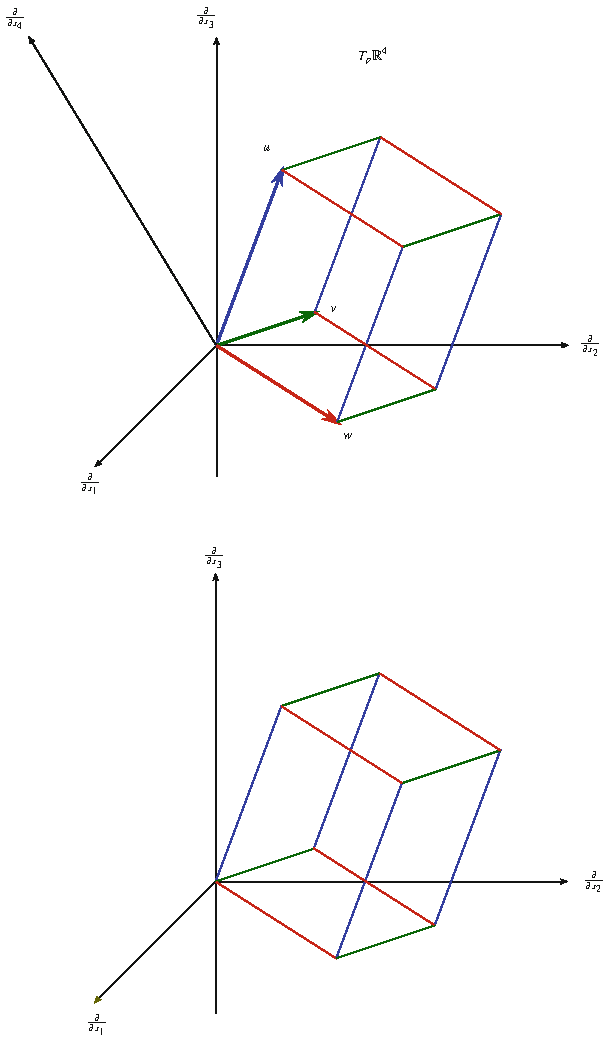
\includegraphics[width=0.729\linewidth]{images/vector/fig-3-16.pdf}
  \caption{图中试图说明切空间 $T_p\mathbb{R}^4$，并画出由 $v_1,v_2,v_3$ 张成的平行六面体（上方）. 3-形式 $dx_1\wedge dx_2\wedge dx_3$ 对三个向量 $u,v,w$ 的作用被表示为该平行六面体到三维 $\partial x_1\partial x_2\partial x_3$ 子空间的投影（下方）}
  \label{fig:3-16}
\end{figure}

\begin{question}\label{q:3-9}
考虑流形 $\mathbb{R}^3$.
\begin{enumerate}
  \item[(a)] 下列哪些是 $\mathbb{R}^3$ 上的 1-形式？
  \begin{enumerate}
    \item[(i)] $3dx_1$
    \item[(ii)] $-4dx_2+7dx_3$
    \item[(iii)] $5dx_1+3dx_2-6dx_1+4dx_3$
    \item[(iv)] $2dx_1\wedge dx_2-4dx_3$
    \item[(v)] $dx_1\wedge dx_2-3dx_2\wedge dx_3$
  \end{enumerate}
  \item[(b)] 下列哪些是 $\mathbb{R}^3$ 上的 2-形式？
  \begin{enumerate}
    \item[(i)] $-4dx_3\wedge dx_2\wedge dx_1$
    \item[(ii)] $6dx_3\wedge dx_2+8dx_3$
    \item[(iii)] $-10dx_1\wedge dx_3+5dx_2\wedge dx_3-dx_1\wedge dx_2$
    \item[(iv)] $-2dx_1\wedge dx_2+3dx_3\wedge dx_2\wedge dx_1$
    \item[(v)] $3dx_1\wedge dx_3-dx_2\wedge dx_3$
  \end{enumerate}
  \item[(c)] 下列哪些是 $\mathbb{R}^3$ 上的 3-形式？
  \begin{enumerate}
    \item[(i)] $5dx_3\wedge dx_2\wedge dx_1$
    \item[(ii)] $-3dx_3\wedge dx_2+2dx_3\wedge dx_1\wedge dx_2$
    \item[(iii)] $5dx_2\wedge dx_3\wedge dx_1+5dx_1\wedge dx_3\wedge dx_2-dx_1\wedge dx_2\wedge dx_3$
    \item[(iv)] $-5dx_3\wedge dx_2+3dx_1\wedge dx_2-dx_3\wedge dx_1$
    \item[(v)] $9dx_1-7dx_2\wedge dx_3$
  \end{enumerate}
\end{enumerate}
\end{question}

\section{n-形式的楔积}

既然我们知道了楔积在几何上做什么，我们就希望能够用代数公式快速处理形式的楔积. 本节我们学习与微分形式有关的一些代数. 首先我们将看到，微分形式基本上遵循我们期望的代数规则，只需稍作调整以适应 $dx_i\wedge dx_j=-dx_j\wedge dx_i$ 这一事实. 之后我们将介绍一点常用记号，然后写出楔积的一个一般公式.

\subsection{代数性质}

设 $\omega,\omega_1,\omega_2$ 是 k-形式，$\eta,\eta_1,\eta_2$ 是 $\ell$-形式. 那么下列性质成立：

\begin{property}{1}\label{prop:3-1}
$(a\omega)\wedge\eta=\omega\wedge(a\eta)=a(\omega\wedge\eta)$，其中 $a\in\mathbb{R}$.
\end{property}

\begin{property}{2}\label{prop:3-2}
$(\omega_1+\omega_2)\wedge\eta=\omega_1\wedge\eta+\omega_2\wedge\eta$.
\end{property}

\begin{property}{3}\label{prop:3-3}
$\omega\wedge(\eta_1+\eta_2)=\omega\wedge\eta_1+\omega\wedge\eta_2$.
\end{property}

\begin{property}{4}\label{prop:3-4}
$\omega\wedge\eta=(-1)^{k\ell}\eta\wedge\omega$.
\end{property}

我们首先通过看 $\mathbb{R}^3$ 上几个简单的例子来说明这些代数性质是合理的. 我们从第一条性质开始，证明 $(adx_1)\wedge dx_2=dx_1\wedge(adx_2)=a(dx_1\wedge dx_2)$. 首先我们有
\begin{align*}
(adx_1)\wedge dx_2(u,v)
&=\begin{vmatrix}
adx_1(u) & adx_1(v)\\
dx_2(u) & dx_2(v)
\end{vmatrix}\\
&=adx_1(u)dx_2(v)-adx_1(v)dx_2(u)\\
&=a\bigl(dx_1(u)dx_2(v)-dx_1(v)dx_2(u)\bigr)\\
&=a\begin{vmatrix}
dx_1(u) & dx_1(v)\\
dx_2(u) & dx_2(v)
\end{vmatrix}\\
&=a\bigl(dx_1\wedge dx_2\bigr)(u,v).
\end{align*}
类似地，
\begin{align*}
dx_1\wedge(adx_2)(u,v)
&=\begin{vmatrix}
dx_1(u) & dx_1(v)\\
adx_2(u) & adx_2(v)
\end{vmatrix}\\
&=adx_1(u)dx_2(v)-adx_1(v)dx_2(u)\\
&=a\bigl(dx_1(u)dx_2(v)-dx_1(v)dx_2(u)\bigr)\\
&=a\begin{vmatrix}
dx_1(u) & dx_1(v)\\
dx_2(u) & dx_2(v)
\end{vmatrix}\\
&=a\bigl(dx_1\wedge dx_2\bigr)(u,v).
\end{align*}
把所有这一切放在一起，不写出向量，就得到我们想要的恒等式. 接下来看一个说明第二条性质的例子；我们证明 $(dx_1+dx_2)\wedge dx_3=dx_1\wedge dx_3+dx_2\wedge dx_3$.
\begin{align*}
\bigl((dx_1+dx_2)\wedge dx_3\bigr)(u,v)
&=\begin{vmatrix}
(dx_1+dx_2)(u) & (dx_1+dx_2)(v)\\
dx_3(u) & dx_3(v)
\end{vmatrix}\\
&=\bigl(dx_1(u)+dx_2(u)\bigr)dx_3(v)-\bigl(dx_1(v)+dx_2(v)\bigr)dx_3(u)\\
&=dx_1(u)dx_3(v)+dx_2(u)dx_3(v)-dx_1(v)dx_3(u)-dx_2(v)dx_3(u)\\
&=dx_1(u)dx_3(v)-dx_1(v)dx_3(u)+dx_2(u)dx_3(v)-dx_2(v)dx_3(u)\\
&=\begin{vmatrix}
dx_1(u) & dx_1(v)\\
dx_3(u) & dx_3(v)
\end{vmatrix}
+\begin{vmatrix}
dx_2(u) & dx_2(v)\\
dx_3(u) & dx_3(v)
\end{vmatrix}\\
&=\bigl(dx_1\wedge dx_3\bigr)(u,v)+\bigl(dx_2\wedge dx_3\bigr)(u,v).
\end{align*}
注意第三条性质 $dx_1\wedge(dx_2+dx_3)=dx_1\wedge dx_2+dx_1\wedge dx_3$ 本质上是相同的.

最后一条性质非常直接. 我们已经知道 $dx_1\wedge dx_2=-dx_2\wedge dx_1$. 事实上，如果 $i\neq j$，我们有 $dx_i\wedge dx_j=-dx_j\wedge dx_i$. 假设我们有一个 3-形式与一个 2-形式楔乘，$(dx_1\wedge dx_2\wedge dx_3)\wedge(dx_4\wedge dx_5)$. 我们要证明
\[
(dx_1\wedge dx_2\wedge dx_3)\wedge(dx_4\wedge dx_5)=(-1)^{3\cdot2}(dx_4\wedge dx_5)\wedge(dx_1\wedge dx_2\wedge dx_3).
\]
这无非是数一下为重新排列各项需要进行多少次交换.

\begin{question}\label{q:3-10}
用六次交换把 $dx_1\wedge dx_2\wedge dx_3\wedge dx_4\wedge dx_5$ 重排为 $dx_4\wedge dx_5\wedge dx_1\wedge dx_2\wedge dx_3$. 例如，从 $dx_1\wedge dx_2\wedge dx_3\wedge dx_4\wedge dx_5$ 变到 $dx_1\wedge dx_2\wedge dx_4\wedge dx_3\wedge dx_5$ 需要一次交换，因此
\[
dx_1\wedge dx_2\wedge dx_3\wedge dx_4\wedge dx_5=-dx_1\wedge dx_2\wedge dx_4\wedge dx_3\wedge dx_5
\]
因为 $dx_3\wedge dx_4=-dx_4\wedge dx_3$.
\end{question}

n 个 1-形式的楔积的一般定义在第 3.1 节中给出：
\[
dx_{i_1}\wedge dx_{i_2}\wedge\cdots\wedge dx_{i_n}(v_1,v_2,\ldots,v_n)\equiv
{\setlength{\arraycolsep}{0.5pt}\begin{vmatrix}
dx_{i_1}(v_1) & dx_{i_1}(v_2) & \cdots & dx_{i_1}(v_n)\\
dx_{i_2}(v_1) & dx_{i_2}(v_2) & \cdots & dx_{i_2}(v_n)\\
\vdots & \vdots & \ddots & \vdots\\
dx_{i_n}(v_1) & dx_{i_n}(v_2) & \cdots & dx_{i_n}(v_n)
\end{vmatrix}},
\]
其中 $v_1,v_2,\ldots,v_n$ 表示向量. 从几何上说，n-形式 $dx_{i_1}\wedge dx_{i_2}\wedge\cdots\wedge dx_{i_n}$ 求出 $v_1,v_2,\ldots,v_n$ 在 $\frac{\partial}{\partial x_{i_1}}\frac{\partial}{\partial x_{i_2}}\cdots\frac{\partial}{\partial x_{i_n}}$-子空间上的投影所张成的平行六面体的体积. 现在回顾我们在第 1.2 节中得到的行列式公式，
\[
\begin{vmatrix}
a_{11} & a_{12} & \cdots & a_{1n}\\
a_{21} & a_{22} & \cdots & a_{2n}\\
\vdots & \vdots & \ddots & \vdots\\
a_{n1} & a_{n2} & \cdots & a_{nn}
\end{vmatrix}
=\sum_{\sigma\in S_n}\mathrm{sgn}(\sigma)\prod_{i=1}^{n}a_{\sigma(i)i},
\]
我们可以把它与 n 个 1-形式的楔积定义结合起来，得到下面关于楔积的重要公式，其中 $S_n$ 是 $n$ 个元素上的置换集：
\[
\text{楔积（n 个 1-形式）：}\quad
dx_{i_1}\wedge dx_{i_2}\wedge\cdots\wedge dx_{i_n}(v_1,v_2,\ldots,v_n)
=\sum_{\sigma\in S_n}\mathrm{sgn}(\sigma)\prod_{j=1}^{n}dx_{\sigma(i_j)}(v_j).
\]
事实上，你偶尔会看到楔积就是用这个公式定义的. 一开始就用这种方式定义楔积的问题在于，完全不清楚这个公式到底在做什么，也不清楚这个定义为什么重要. 至少我们现在彻底理解了楔积到底求出什么. 用这个公式来实际证明本节的代数性质并不困难，如下面的问题所示.

\begin{question}\label{q:3-11}
设 $\omega=a\,dx_{i_1}\wedge\cdots\wedge dx_{i_k}$，$\eta=b\,dx_{i_{k+1}}$，其中 $a,b\in\mathbb{R}$. 利用 n 个 1-形式的楔积公式以及类似于上面例子的步骤，证明
\[
\omega\wedge\eta=ab\,dx_{i_1}\wedge\cdots\wedge dx_{i_k}\wedge dx_{i_{k+1}}.
\]
\end{question}

\begin{question}\label{q:3-12}
设 $\omega_1=a_1dx_{i_1}\wedge\cdots\wedge dx_{i_k}$、$\omega_2=a_2dx_{j_1}\wedge\cdots\wedge dx_{j_k}$，$\eta=b\,dx_{i_{k+1}}$. 利用 n 个 1-形式的楔积公式证明
\[
(\omega_1+\omega_2)\wedge\eta=\omega_1\wedge\eta+\omega_2\wedge\eta.
\]
解释这如何也蕴含 $\omega\wedge(\eta_1+\eta_2)=\omega\wedge\eta_1+\omega\wedge\eta_2$.
\end{question}

\begin{question}\label{q:3-13}
设 $\omega=dx_{i_1}\wedge\cdots\wedge dx_{i_k}$，$\eta=dx_{j_1}\wedge\cdots\wedge dx_{j_\ell}$. 证明
\[
\omega\wedge\eta=(-1)^{k\ell}\eta\wedge\omega.
\]
\end{question}

\begin{question}\label{q:3-14}
设 $\omega,\omega_1,\omega_2$ 是 k-形式，$\eta,\eta_1,\eta_2$ 是 $\ell$-形式. 利用上面三个问题，补全本节代数性质的证明：
\begin{enumerate}
  \item[(1)] $(a\omega)\wedge\eta=\omega\wedge(a\eta)=a(\omega\wedge\eta)$，其中 $a\in\mathbb{R}$，
  \item[(2)] $(\omega_1+\omega_2)\wedge\eta=\omega_1\wedge\eta+\omega_2\wedge\eta$，
  \item[(3)] $\omega\wedge(\eta_1+\eta_2)=\omega\wedge\eta_1+\omega\wedge\eta_2$，
  \item[(4)] $\omega\wedge\eta=(-1)^{k\ell}\eta\wedge\omega$.
\end{enumerate}
\end{question}

\subsection{简化记号}

在上一节中我们考察了 $\mathbb{R}^2$ 上的 2-形式，记为 $\Lambda^2(\mathbb{R}^3)$，并发现 $dx_1\wedge dx_2$、$dx_2\wedge dx_3$ 与 $dx_3\wedge dx_1$ 是 $\Lambda^2(\mathbb{R}^3)$ 的一组基. 因此，任意 2-形式 $\alpha\in\Lambda^2(\mathbb{R}^3)$ 都具有
\[
\alpha=a_{12}dx_1\wedge dx_2+a_{23}dx_2\wedge dx_3+a_{31}dx_3\wedge dx_1
\]
的形式，其中 $a_{12}$、$a_{23}$ 与 $a_{31}$ 只是 $\mathbb{R}$ 中的常数. 我们同样可以像上一节那样写成
\[
\alpha=adx_1\wedge dx_2+bdx_2\wedge dx_3+cdx_3\wedge dx_1
\]
甚至写成
\[
\alpha=a_1dx_1\wedge dx_2+a_2dx_2\wedge dx_3+a_3dx_3\wedge dx_1.
\]
毕竟，我们给常数起什么名字又有什么关系呢？但事实证明，用出现在其后的基元素中的那些数字来给常数编指标在记号上是方便的. 回忆一下，我们把 $\mathbb{R}^3$ 上 2-形式基元素的指标写成循环次序，这意味着我们写 $dx_3\wedge dx_1$ 而不是 $dx_1\wedge dx_3$. 这是向量微积分中的约定. 但对于 $n>3$ 的流形 $\mathbb{R}^n$，这个约定不再适用，我们就简单地按递增次序写指标. 如果 $\alpha\in\Lambda^2(\mathbb{R}^4)$，我们会写
\[
\alpha=a_{12}dx_1\wedge dx_2+a_{13}dx_1\wedge dx_3+a_{14}dx_1\wedge dx_4
+a_{23}dx_2\wedge dx_3+a_{24}dx_2\wedge dx_4+a_{34}dx_3\wedge dx_4.
\]
$\Lambda^3(\mathbb{R}^4)$ 的基元素是
\[
dx_1\wedge dx_2\wedge dx_3,\qquad
dx_1\wedge dx_2\wedge dx_4,\qquad
dx_1\wedge dx_3\wedge dx_4,\qquad
dx_2\wedge dx_3\wedge dx_4.
\]
再次注意，指标全部按递增次序排列. 任意 3-形式 $\alpha\in\Lambda^3(\mathbb{R}^4)$ 会被写成
\[
\alpha=a_{123}dx_1\wedge dx_2\wedge dx_3+a_{124}dx_1\wedge dx_2\wedge dx_4
+a_{134}dx_1\wedge dx_3\wedge dx_4+a_{234}dx_2\wedge dx_3\wedge dx_4.
\]
对于 $\Lambda^k(\mathbb{R}^n)$ 中的任意 k-形式，我们不想真的写出 $\Lambda^k(\mathbb{R}^n)$ 的基的所有元素，因此我们改写成
\[
\alpha=\sum_{I}a_I\,dx^I.
\]
这里 $I$ 代表集合中递增指标 $i_1i_2\ldots i_k$（其中 $1\leq i_1<i_2<\cdots<i_k\leq n$）的元素. 即
\[
I\in I_{k,n}=\Bigl\{(i_1i_2\ldots i_k)\;\Big|\;1\leq i_1<i_2<\cdots<i_k\leq n\Bigr\}.
\]
所以，对 $k=2,n=4$，我们有
\[
I\in I_{2,4}=\{12,13,14,23,24,34\}
\]
而对 $k=3,n=4$，我们有
\[
I\in I_{3,4}=\{123,124,134,234\}.
\]
在这种记号中，有 $dx^{12}\equiv dx_1\wedge dx_2$、$dx^{24}\equiv dx_2\wedge dx_4$、$dx^{134}\equiv dx_1\wedge dx_3\wedge dx_4$，等等. 如果你想知道为什么左边的指标是上标而右边的指标是下标，这是因为这种记号与 Einstein 求和记号兼容. 我们将在第 9.4 节解释 Einstein 求和记号. 目前先不必担心它.

假设我们有 $\alpha\in\Lambda^k(\mathbb{R}^n)$ 与 $\beta\in\Lambda^\ell(\mathbb{R}^n)$，其中 $\alpha=\sum_{I}a_I\,dx^I$，$\beta=\sum_{J}b_J\,dx^J$. 那么 $\alpha\wedge\beta$ 由下式给出：
\[
\text{两个任意形式的楔积，公式一：}\qquad
\left(\sum_{I}a_I\,dx^I\right)\wedge\left(\sum_{J}b_J\,dx^J\right)
=\sum_{I,J}a_Ib_J\,dx^I\wedge dx^J.
\]
在右边的求和中，如果 $I$ 与 $J$ 有任何公共指标，就有 $dx^I\wedge dx^J=0$.

\begin{question}\label{q:3-15}
设 $\alpha=\sum_{I}a_I\,dx^I\in\Lambda^k(\mathbb{R}^n)$，$\beta=\sum_{J}b_J\,dx^J\in\Lambda^\ell(\mathbb{R}^n)$. 通过反复应用楔积的代数性质，证明这两个任意形式的楔积公式.
\end{question}

如果 $I$ 与 $J$ 不相交，那么 $dx^I\wedge dx^J=\pm dx^K$，其中 $K=I\cup J$，但要重排为递增次序，并删去重复出现的指标的元素. 因此公式一自动给出公式二：
\begin{align*}
&\text{两个任意形式的楔积，公式二：}\\
\left(\sum_{I}a_I\,dx^I\right)\wedge\left(\sum_{J}b_J\,dx^J\right)
&=\sum_{K}\left(\sum_{\substack{I\cup J=K\\I,J\text{ 不相交}}}\pm a_Ib_J\right)dx^K.
\end{align*}

一个例子应该有助于把这一点弄得更清楚. 设 $\alpha$ 与 $\beta$ 是 $\mathbb{R}^8$ 上的如下形式：
\begin{align*}
\alpha=5dx_1\wedge dx_2-6dx_2\wedge dx_4+7dx_1\wedge dx_7+2dx_2\wedge dx_8, \\
\beta=3dx_3\wedge dx_5\wedge dx_8-4dx_5\wedge dx_6\wedge dx_8.
\end{align*}
于是我们有 $\alpha=\sum_{I}a_I\,dx^I$，其中 $I$ 是集合 $\{12,24,17,28\}\subset I_{2,8}$ 的元素，系数为 $a_{12}=5$、$a_{24}=-6$、$a_{17}=7$、$a_{28}=2$. 类似地，我们有 $\beta=\sum_{J}b_J\,dx^J$，其中 $J$ 是集合 $\{358,568\}\subset I_{3,8}$ 的元素，系数为 $b_{358}=3$、$b_{568}=-4$. 那么，我们的元素 $K$ 是什么呢？它们由集合 $I\cup J$ 给出，但要重排为递增次序，并删去有重复指标的元素. 首先我们有
\[
I\cup J=\{12358,\;24358,\;17358,\;28358,\;12568,\;24568,\;17568,\;28568\}.
\]
我们注意到的第一件事是，这个集合中有两个元素的指标是重复的. $28358$ 与 $28568$ 都重复了 8. 由于 $dx_2\wedge dx_8\wedge dx_3\wedge dx_5\wedge dx_8=0$ 且 $dx_2\wedge dx_8\wedge dx_5\wedge dx_6\wedge dx_8=0$，我们可以删去这两个元素.

为了得到 $K$，我们需要把其余指标集合按递增次序排列. 第一个元素 $12358$ 已经是递增次序，所以不需要做任何事. $dx^{12358}$ 前面的系数就是 $a_{12}b_{358}$. 要把 $24358$ 排成递增次序，我们只需做一次交换，即交换 4 与 3 得到 $23458$. 这一次交换给出一个负号，它出现在 $dx^{23458}$ 前面的系数中，即 $-a_{24}b_{358}=-(-6)(3)=18$. 其他项也类似. 因此我们最终得到
\[
K=\{12358,\;23458,\;13578,\;\overline{23588},\;12568,\;24568,\;15678,\;\overline{25688}\}.
\]
注意，我们定义 $K$ 的方式意味着我们并不跟踪为把指标排成次序而进行交换时发生的符号变化. 这就是为什么写 $dx^I\wedge dx^J=\pm dx^K$ 时会有 $\pm$.

\begin{question}\label{q:3-16}
完成 $\alpha\wedge\beta$ 的书写.
\end{question}

\begin{question}\label{q:3-17}
设
\[
\alpha=4dx_1\wedge dx_3+5dx_3\wedge dx_5-7dx_3\wedge dx_9
\]
是 $\mathbb{R}^9$ 上的 2-形式，设
\[
\beta=7dx_1\wedge dx_4\wedge dx_6\wedge dx_8-3dx_2\wedge dx_3\wedge dx_7\wedge dx_9+dx_5\wedge dx_6\wedge dx_8\wedge dx_9
\]
是 $\mathbb{R}^9$ 上的 4-形式. 求 $\alpha\wedge\beta$，然后求 $\beta\wedge\alpha$.
\end{question}

从前面的问题你可以看到，实际使用这个公式意味着我们要做大量工作来重排 $I$ 与 $J$ 的系数以得到 $K$，并找出正确的符号. 这个公式真正派上用场的地方，是在做一般计算（而不是处理具体例子）时，我们并不太担心楔积的具体形式.

\subsection{一般公式}

本节引入两个任意形式的楔积的几个新公式. 事实上，下面三个一般公式经常被作为楔积的定义遇到. 本节我们将深入讨论其中两个公式. 第三个只是为了完整起见而放在这里. 设 $\alpha$ 是 k-形式，$\beta$ 是 $\ell$-形式. 那么 $\alpha$ 与 $\beta$ 的楔积由下式给出：
\begin{align*}
&\text{两个任意形式的楔积，公式三：}\\
&(\alpha\wedge\beta)(v_1,\ldots,v_{k+\ell})\\
&=\frac{1}{k!\,\ell!}\sum_{\sigma\in S_{k+\ell}}\mathrm{sgn}(\sigma)\alpha\bigl(v_{\sigma(1)},\ldots,v_{\sigma(k)}\bigr)\\
&\qquad\cdot\beta\bigl(v_{\sigma(k+1)},\ldots,v_{\sigma(k+\ell)}\bigr),
\end{align*}
它也可以写成
\begin{align*}
&\text{两个任意形式的楔积，公式四：}\\
&(\alpha\wedge\beta)(v_1,\ldots,v_{k+\ell})\\
&=\sum_{\substack{\sigma\text{ 是}\\ (k,\ell)\text{-洗牌}}}\mathrm{sgn}(\sigma)\alpha\bigl(v_{\sigma(1)},\ldots,v_{\sigma(k)}\bigr)\\
&\qquad\cdot\beta\bigl(v_{\sigma(k+1)},\ldots,v_{\sigma(k+\ell)}\bigr).
\end{align*}
在那些先引入张量、然后把微分形式定义为某种张量的书中，楔积常常由公式
\[
\text{两个任意形式的楔积，公式五：}\qquad
\alpha\wedge\beta=\frac{(k+\ell)!}{k!\,\ell!}\,\mathcal{A}(\alpha\otimes\beta)
\]
定义，其中 $\otimes$ 是张量积，$\mathcal{A}$ 是反对称化（或反称化）算子. 对这个特定定义的解释在关于张量的附录第 A.5 节中给出.

我们现在把注意力转向理解公式三与公式四，并看出它们确实与我们基于体积/行列式的楔积定义相同. 第一步是证明公式三与公式四的右边彼此相等. 一旦做到这一点，我们将证明这些公式实际上可以从我们关于 n 个 1-形式的楔积定义推导出来，从而也可以用作定义楔积的方程；也就是说，我们将证明这些公式确实是 $(\alpha\wedge\beta)(v_1,\ldots,v_{k+\ell})$ 的公式.

首先考虑公式三右边给出的公式：
\[
\frac{1}{k!\,\ell!}\sum_{\sigma\in S_{k+\ell}}\mathrm{sgn}(\sigma)\alpha\bigl(v_{\sigma(1)},\ldots,v_{\sigma(k)}\bigr)\beta\bigl(v_{\sigma(k+1)},\ldots,v_{\sigma(k+\ell)}\bigr).
\]
开头的因子 $\frac{1}{k!\,\ell!}$ 从何而来？考虑置换 $\sigma\in S_{k+\ell}$. 在 $S_{k+\ell}$ 中有 $k!$ 个不同的置换 $\tau$，它们置换前 $k$ 项但保持项 $k+1,\ldots,k+\ell$ 不动. 这意味着对任意置换 $\sigma$，我们有 $\sigma\tau(k+1)=\sigma(k+1),\ldots,\sigma\tau(k+\ell)=\sigma(k+\ell)$. 这意味着我们有
\begin{align*}
&\mathrm{sgn}(\sigma\tau)\alpha\bigl(v_{\sigma\tau(1)},\ldots,v_{\sigma\tau(k)}\bigr)\beta\bigl(v_{\sigma\tau(k+1)},\ldots,v_{\sigma\tau(k+\ell)}\bigr)\\
&=\mathrm{sgn}(\sigma)\mathrm{sgn}(\tau)\alpha\bigl(v_{\sigma(1)},\ldots,v_{\sigma(k)}\bigr)\beta\bigl(v_{\sigma(k+1)},\ldots,v_{\sigma(k+\ell)}\bigr)\\
&=\mathrm{sgn}(\sigma)\underbrace{\mathrm{sgn}(\tau)\mathrm{sgn}(\tau)}_{=1}\alpha\bigl(v_{\sigma(1)},\ldots,v_{\sigma(k)}\bigr)\beta\bigl(v_{\sigma(k+1)},\ldots,v_{\sigma(k+\ell)}\bigr)\\
&=\mathrm{sgn}(\sigma)\alpha\bigl(v_{\sigma(1)},\ldots,v_{\sigma(k)}\bigr)\beta\bigl(v_{\sigma(k+1)},\ldots,v_{\sigma(k+\ell)}\bigr)
\end{align*}
其中第一个等号来自以下事实：$\tau(1),\ldots,\tau(k)$ 只是 $1,\ldots,k$ 的一个置换，因此
\[
\alpha\bigl(v_{\sigma\tau(1)},\ldots,v_{\sigma\tau(k)}\bigr)=\mathrm{sgn}(\tau)\alpha\bigl(v_{\sigma(1)},\ldots,v_{\sigma(k)}\bigr).
\]
此外，$\sigma\tau$ 固定最后 $\ell$ 项，于是
\[
\beta\bigl(v_{\sigma\tau(k+1)},\ldots,v_{\sigma\tau(k+\ell)}\bigr)=\beta\bigl(v_{\sigma(k+1)},\ldots,v_{\sigma(k+\ell)}\bigr).
\]
这意味着，给定一个特定的 $\sigma$，在和
\[
\sum_{\sigma\in S_{k+\ell}}\mathrm{sgn}(\sigma)\alpha\bigl(v_{\sigma(1)},\ldots,v_{\sigma(k)}\bigr)\beta\bigl(v_{\sigma(k+1)},\ldots,v_{\sigma(k+\ell)}\bigr)
\]
中还有 $k!$ 个其他项与之完全相同. 我们除以 $k!$ 来消除这 $k!$ 个重复项.

类似地，给定置换 $\sigma\in S_{k+\ell}$，在 $S_{k+\ell}$ 中有 $\ell!$ 个不同的置换 $\tau$，它们置换最后 $\ell$ 项但保持项 $1,\ldots,k$ 不动. 一个完全相同的论证表明，我们还需要除以 $\ell!$ 来消除这 $\ell!$ 个重复项. 因此因子 $\frac{1}{k!\,\ell!}$ 消除了对 $\sigma\in S_{k+\ell}$ 求和中的所有重复项. 这意味着我们关于楔积的第一个定义的右边消除了所有重复项.

接下来，我们来看
\[
\begin{aligned}
&\frac{1}{k!\,\ell!}\sum_{\sigma\in S_{k+\ell}}\mathrm{sgn}(\sigma)\alpha\bigl(v_{\sigma(1)},\ldots,v_{\sigma(k)}\bigr)\\
&\qquad\cdot\beta\bigl(v_{\sigma(k+1)},\ldots,v_{\sigma(k+\ell)}\bigr)\\
&=\sum_{\substack{\sigma\text{ 是}\\ (k,\ell)\text{-洗牌}}}\mathrm{sgn}(\sigma)\alpha\bigl(v_{\sigma(1)},\ldots,v_{\sigma(k)}\bigr)\\
&\qquad\cdot\beta\bigl(v_{\sigma(k+1)},\ldots,v_{\sigma(k+\ell)}\bigr).
\end{aligned}
\]
称置换 $\sigma\in S_{k+\ell}$ 为 $(k,\ell)$-洗牌，若 $\sigma(1)<\cdots<\sigma(k)$ 且 $\sigma(k+1)<\cdots<\sigma(k+\ell)$. \newterm{shuffle}{洗牌}{shuffle} 一词的意思如下：置换的前 $k$ 项按递增次序排列，并且后 $\ell$ 项也按递增次序排列.

\begin{question}\label{q:3-18}
求 $1\;2\;3\;4\;5$ 的 $(2,3)$-洗牌.
\end{question}

当我们在左边对 $\sigma\in S_{k+\ell}$ 求和时，对每一个这样的 $\sigma$，还有 $k!\,\ell!-1$ 个给出相同项的其他置换. 这本质上就是我们刚刚进行的同一个论证. 在给出相同项的这 $k!\,\ell!$ 个不同置换中，恰好有一个是 $(k,\ell)$-洗牌. 因此，通过选取那个是 $(k,\ell)$-洗牌的特定置换，我们实际上是在从 $k!\,\ell!$ 个相同项中选取一个代表置换. 所以当我们对所有 $(k,\ell)$-洗牌求和时，我们只是从对 $\sigma\in S_{k+\ell}$ 求和时出现的每组相同项中各取一项来求和，从而无需再除以 $k!\,\ell!$. 因此我们证明了，两个微分形式楔积的公式三与公式四的右边确实相等.

\begin{question}\label{q:3-19}
补全这个论证的细节.
\end{question}

现在我们将证明公式四的右边确实等于公式四的左边. 一旦做到这一点，公式三就由上面的结果自动推出. 在真正做一般情形之前，我们先对一个简单的例子证明它成立. 考虑 $\alpha=dx_2\wedge dx_3\in\Lambda^2(\mathbb{R}^5)$ 与 $\beta=dx_5\in\Lambda^1(\mathbb{R}^5)$. 我们首先用基于体积/行列式的楔积定义计算 $\alpha\wedge\beta(v_1,v_2,v_3)$. 然后我们把公式四的右边应用于 $\alpha$ 与 $\beta$，从而看出它们相等，这正是我们要证明的.

首先，我们用基于体积/行列式的定义写出 $\alpha\wedge\beta(v_1,v_2,v_3)$：
\begin{align*}
\alpha\wedge\beta(v_1,v_2,v_3)
&=dx_2\wedge dx_3\wedge dx_5(v_1,v_2,v_3)\\
&=\begin{vmatrix}
dx_2(v_1) & dx_2(v_2) & dx_2(v_3)\\
dx_3(v_1) & dx_3(v_2) & dx_3(v_3)\\
dx_5(v_1) & dx_5(v_2) & dx_5(v_3)
\end{vmatrix}\\
&=dx_2(v_1)dx_3(v_2)dx_5(v_3)+dx_2(v_2)dx_3(v_3)dx_5(v_1)\\
&\quad+dx_2(v_3)dx_3(v_1)dx_5(v_2)-dx_2(v_3)dx_3(v_2)dx_5(v_1)\\
&\quad-dx_2(v_2)dx_3(v_1)dx_5(v_3)-dx_2(v_1)dx_3(v_3)dx_5(v_2)\\
&=\bigl(dx_2\,dx_3\,dx_5+dx_5\,dx_2\,dx_3+dx_3\,dx_5\,dx_2\\
&\qquad-dx_5\,dx_3\,dx_2-dx_3\,dx_2\,dx_5-dx_2\,dx_5\,dx_3\bigr)(v_1,v_2,v_3).
\end{align*}

现在我们将使用公式四的右边，求 $\sum_{\sigma}\mathrm{sgn}(\sigma)\alpha(v_{\sigma(1)},v_{\sigma(2)})\beta(v_{\sigma(3)})$，其中 $\sigma$ 是 $(2,1)$-洗牌. $123$ 的 $(2,1)$-洗牌是 $231$、$132$ 与 $123$. 因此我们有三个 $(2,1)$-洗牌置换
\[
\sigma_1=\begin{pmatrix}1&2&3\\2&3&1\end{pmatrix},\qquad
\sigma_2=\begin{pmatrix}1&2&3\\1&3&2\end{pmatrix},\qquad
\sigma_3=\begin{pmatrix}1&2&3\\1&2&3\end{pmatrix}.
\]
容易证明 $\mathrm{sgn}(\sigma_1)$ 与 $\mathrm{sgn}(\sigma_3)$ 是正的，$\mathrm{sgn}(\sigma_2)$ 是负的，因此
\begin{align*}
\alpha\wedge\beta(v_1,v_2,v_3)
&=\sum_{\substack{\sigma\text{ 是}\\ (2,1)\text{-洗牌}}}\mathrm{sgn}(\sigma)(dx_2\wedge dx_3)(v_{\sigma(1)},v_{\sigma(2)})dx_5(v_{\sigma(3)})\\
&=(dx_2\wedge dx_3)(v_2,v_3)dx_5(v_1)-(dx_2\wedge dx_3)(v_1,v_3)dx_5(v_2)\\
&\quad+(dx_2\wedge dx_3)(v_1,v_2)dx_5(v_3)\\
&=\begin{vmatrix}
dx_2(v_2) & dx_2(v_3)\\
dx_3(v_2) & dx_3(v_3)
\end{vmatrix}dx_5(v_1)
-\begin{vmatrix}
dx_2(v_1) & dx_2(v_3)\\
dx_3(v_1) & dx_3(v_3)
\end{vmatrix}dx_5(v_2)\\
&\quad+\begin{vmatrix}
dx_2(v_1) & dx_2(v_2)\\
dx_3(v_1) & dx_3(v_2)
\end{vmatrix}dx_5(v_3)\\
&=dx_2(v_2)dx_3(v_3)dx_5(v_1)-dx_2(v_3)dx_3(v_2)dx_5(v_1)\\
&\quad-dx_2(v_1)dx_3(v_3)dx_5(v_2)+dx_2(v_3)dx_3(v_1)dx_5(v_2)\\
&\quad+dx_2(v_1)dx_3(v_2)dx_5(v_3)-dx_2(v_2)dx_3(v_1)dx_5(v_3)\\
&=\bigl(dx_5\,dx_2\,dx_3-dx_5\,dx_3\,dx_2-dx_2\,dx_5\,dx_3\\
&\qquad+dx_3\,dx_5\,dx_2+dx_2\,dx_3\,dx_5-dx_3\,dx_2\,dx_5\bigr)(v_1,v_2,v_3).
\end{align*}
重新排列后可以看出，确实，用基于体积/行列式的楔积定义求出的 $\alpha\wedge\beta(v_1,v_2,v_3)$，与我们使用公式四的右边（$\sum_{\sigma}\mathrm{sgn}(\sigma)\alpha(v_{\sigma(1)},v_{\sigma(2)})\beta(v_{\sigma(3)})$，其中 $\sigma$ 是 $(2,1)$-洗牌）得到的结果完全相同. 因此，确实有 $\alpha\wedge\beta(v_1,v_2,v_3)=\sum_{\sigma}\mathrm{sgn}(\sigma)\alpha(v_{\sigma(1)},v_{\sigma(2)})\beta(v_{\sigma(3)})$，其中 $\sigma$ 是 $(2,1)$-洗牌.

现在我们把注意力转向一般情形. 我们用来证明这一点的步骤将模仿上面的例子. 我们想对一个 k-形式 $\alpha\in\Lambda^k(\mathbb{R}^n)$ 与 $\ell$-形式 $\beta\in\Lambda^\ell(\mathbb{R}^n)$ 证明这个等式. 一般来说，我们有 $\alpha=\sum_{I}a_I\,dx^I$ 与 $\beta=\sum_{J}b_J\,dx^J$，其中
\begin{align*}
I\in I_{k,n}=\Bigl\{i_1i_2\cdots i_k\;\Big|\;1\leq i_1<i_2<\cdots<i_k\leq n\Bigr\}, \\
J\in J_{\ell,n}=\Bigl\{j_1j_2\cdots j_\ell\;\Big|\;1\leq j_1<j_2<\cdots<j_\ell\leq n\Bigr\}.
\end{align*}
首先要注意的是，我们基于体积/行列式的楔积定义只适用于形如 $dx_{i_1}\wedge dx_{i_2}\wedge\cdots\wedge dx_{i_m}$ 的元素，即 $\Lambda^m(\mathbb{R}^n)$ 的基元素. 如果我们有一个一般的 k-形式，比如 $\alpha=\sum_{I}a_I\,dx^I$，并且想用这个定义来求 $\alpha(v_1,\ldots,v_k)$，我们首先必须对每个 $I$ 通过取投影向量的行列式求出 $dx^I(v_1,\ldots,v_k)=dx_{i_1}\wedge\cdots\wedge dx_{i_k}(v_1,\ldots,v_k)$ 的值，把我们求出的值乘以系数 $a_I$，然后把所有项加起来. 对 $\beta$ 也类似.

取 $\alpha$ 与 $\beta$ 的楔积，并使用上一节证明的公式一，我们有
\begin{align*}
\alpha\wedge\beta
&=\left(\sum_{I}a_I\,dx^I\right)\wedge\left(\sum_{J}b_J\,dx^J\right)\\
&=\sum_{I,J}a_Ib_J\,dx^I\wedge dx^J\\
&=\sum_{I,J}a_Ib_J\,dx_{i_1}\wedge\cdots\wedge dx_{i_k}\wedge dx_{j_1}\wedge\cdots\wedge dx_{j_\ell}.
\end{align*}
所以，使用我们基于体积/行列式的楔积定义，我们有
\begin{align*}
\alpha\wedge\beta(v_1,\cdots,v_{k+\ell})
&=\sum_{I,J}a_Ib_J\,dx_{i_1}\wedge\cdots\wedge dx_{i_k}\wedge dx_{j_1}\wedge\cdots\wedge dx_{j_\ell}(v_1,\cdots,v_{k+\ell})\\
&=\sum_{I}a_I\,dx_{i_1}\wedge\cdots\wedge dx_{i_k}\wedge dx_{i_{k+1}}\wedge\cdots\wedge dx_{i_{k+\ell}}(v_1,\cdots,v_{k+\ell})\\
&=\sum_{I}a_I\\
&\,\cdot\sum_{\sigma\in S_{k+\ell}}\mathrm{sgn}(\sigma)\\
&\,\cdot\prod_{m=1}^{k+\ell}dx_{i_{\sigma(m)}}(v_m),
\end{align*}
其中我们在第二个等号中做了记号改变 $I=I\cup J$，以使指标标签整齐地对齐. 因此 $j_1=i_{k+1},\ldots,j_\ell=i_{k+\ell}$，而 $a_I$ 项是适当的 $a_Ib_J$ 项；即 $a_{i_1\cdots i_{k+\ell}}=a_{i_1\cdots i_k}b_{j_1\cdots j_\ell}$.

现在，使用我们的 $(k,\ell)$-洗牌公式，我们有
\begin{align*}
&\sum_{\substack{\sigma\text{ 是}\\ (k,\ell)\text{-洗牌}}}\mathrm{sgn}(\sigma)\alpha(v_{\sigma(1)},\cdots,v_{\sigma(k)})\beta(v_{\sigma(k+1)},\cdots,v_{\sigma(k+\ell)})\\
&=\sum_{\substack{\sigma\text{ 是}\\ (k,\ell)\text{-洗牌}}}\mathrm{sgn}(\sigma)
\left(\sum_{I}a_I\,dx^I(v_{\sigma(1)},\cdots,v_{\sigma(k)})\right)
\left(\sum_{J}b_J\,dx^J(v_{\sigma(k+1)},\cdots,v_{\sigma(k+\ell)})\right)\\
&=\sum_{\substack{\sigma\text{ 是}\\ (k,\ell)\text{-洗牌}}}\mathrm{sgn}(\sigma)
\sum_{I,J}a_Ib_J\,dx^I(v_{\sigma(1)},\cdots,v_{\sigma(k)})dx^J(v_{\sigma(k+1)},\cdots,v_{\sigma(k+\ell)})\\
&=\sum_{I}a_I\sum_{\substack{\sigma\text{ 是}\\ (k,\ell)\text{-洗牌}}}\mathrm{sgn}(\sigma)
dx_{i_1}\wedge\cdots\wedge dx_{i_k}(v_{\sigma(1)},\cdots,v_{\sigma(k)})\\
&\qquad\qquad\cdot\;dx_{i_{k+1}}\wedge\cdots\wedge dx_{i_{k+\ell}}(v_{\sigma(k+1)},\cdots,v_{\sigma(k+\ell)}),
\end{align*}
其中在最后一个等号中我们做了与前面相同的记号改变，并交换了求和次序. 我们的目标是看出这与前面的公式中基于体积/行列式的定义给出的结果完全相同.

首先，利用行列式的楔积定义，我们有
\[
dx_{i_1}\wedge\cdots\wedge dx_{i_k}(v_{\sigma(1)},\cdots,v_{\sigma(k)})
=\sum_{\tilde{\sigma}\in S_k}\mathrm{sgn}(\tilde{\sigma})\prod_{m=1}^{k}dx_{i_{\tilde{\sigma}(m)}}(v_{\sigma(m)})
\]
与
\[
dx_{i_{k+1}}\wedge\cdots\wedge dx_{i_{k+\ell}}(v_{\sigma(k+1)},\cdots,v_{\sigma(k+\ell)})
=\sum_{\tilde{\tilde{\sigma}}\in S_\ell}\mathrm{sgn}(\tilde{\tilde{\sigma}})\prod_{m=k+1}^{k+\ell}dx_{i_{\tilde{\tilde{\sigma}}(m)}}(v_{\sigma(m)}).
\]
把它们结合起来，我们有
\begin{align*}
&\sum_{I}a_I\sum_{\substack{\sigma\text{ 是}\\ (k,\ell)\text{-洗牌}}}\mathrm{sgn}(\sigma)
dx_{i_1}\wedge\cdots\wedge dx_{i_k}(v_{\sigma(1)},\cdots,v_{\sigma(k)})\\
&\qquad\qquad\qquad\qquad\;\cdot\;dx_{i_{k+1}}\wedge\cdots\wedge dx_{i_{k+\ell}}(v_{\sigma(k+1)},\cdots,v_{\sigma(k+\ell)})\\
&=\sum_{I}a_I\sum_{\substack{\sigma\text{ 是}\\ (k,\ell)\text{-洗牌}}}\mathrm{sgn}(\sigma)
\left(\sum_{\tilde{\sigma}\in S_k}\mathrm{sgn}(\tilde{\sigma})\prod_{m=1}^{k}dx_{i_{\tilde{\sigma}(m)}}(v_{\sigma(m)})\right)\\
&\qquad\qquad\cdot
\left(\sum_{\tilde{\tilde{\sigma}}\in S_\ell}\mathrm{sgn}(\tilde{\tilde{\sigma}})\prod_{m=k+1}^{k+\ell}dx_{i_{\tilde{\tilde{\sigma}}(m)}}(v_{\sigma(m)})\right)\\
&=\sum_{I}a_I\sum_{\substack{\sigma\text{ 是}\\ (k,\ell)\text{-洗牌}}}\;\sum_{\tilde{\sigma}\in S_k}\;\sum_{\tilde{\tilde{\sigma}}\in S_\ell}
\mathrm{sgn}(\sigma)\mathrm{sgn}(\tilde{\sigma})\mathrm{sgn}(\tilde{\tilde{\sigma}})\\
&\qquad\qquad\qquad\qquad\left(\prod_{m=1}^{k}dx_{i_{\tilde{\sigma}(m)}}(v_{\sigma(m)})\right)\\
&\qquad\qquad\cdot\left(\prod_{m=k+1}^{k+\ell}dx_{i_{\tilde{\tilde{\sigma}}(m)}}(v_{\sigma(m)})\right)\\
&=\sum_{I}a_I\\
&\,\cdot\sum_{\sigma\in S_{k+\ell}}\mathrm{sgn}(\sigma)\\
&\,\cdot\prod_{m=1}^{k+\ell}dx_{i_{\sigma(m)}}(v_m),
\end{align*}
这与基于体积/行列式的定义给出的 $\alpha\wedge\beta(v_1,\cdots,v_{k+\ell})$ 完全相同. 因此，公式四确实是 $\alpha\wedge\beta(v_1,\cdots,v_{k+\ell})$ 的公式. 公式三随之而来. 要让自己确信最后一个等号，可能需要稍微思考一下.

\begin{question}\label{q:3-20}
解释上面的最后一个等号.
\end{question}

\section{内积}

我们现在引入一个称为向量与 k-形式的\newterm{interior-product}{内积}{interior product}（inner product）的东西. 给定向量 $v$ 与 k-形式 $\alpha$，$v$ 与 $\alpha$ 的内积记为 $\iota_v\alpha$. k-形式 $\alpha$ 与向量 $v$ 的内积是一个由下式定义的 $(k-1)$-形式：
\[
\text{内积：}\qquad\iota_v\alpha(v_1,\ldots,v_{k-1})=\alpha(v,v_1,\ldots,v_{k-1}).
\]
其中 $v_1,\ldots,v_{k-1}$ 是任意 $k-1$ 个向量. 换句话说，$\iota_v\alpha$ 只是把向量 $v$ 放进 $\alpha$ 的第一个槽位. 所以，当 $\alpha$ 是 k-形式时，$\iota_v\alpha$ 是 $(k-1)$-形式.

现在我们指出一个简单的恒等式. 如果 $\alpha$ 与 $\beta$ 都是 k-形式，那么
\[
\iota_v(\alpha+\beta)=\iota_v\alpha+\iota_v\beta.
\]
这直接来自形式求和的计算方式：
\begin{align*}
\iota_v(\alpha+\beta)(v_1,\ldots,v_{k-1})
&=(\alpha+\beta)(v,v_1,\ldots,v_{k-1})\\
&=\alpha(v,v_1,\ldots,v_{k-1})+\beta(v,v_1,\ldots,v_{k-1})\\
&=\iota_v\alpha(v_1,\ldots,v_{k-1})+\iota_v\beta(v_1,\ldots,v_{k-1}),
\end{align*}
这就给出了这个恒等式. 现在设 $\alpha$ 是 k-形式，$v,w$ 是向量. 我们还有
\[
\iota_{(v+w)}\alpha=\iota_v\alpha+\iota_w\alpha.
\]
因此内积 $\iota_v\alpha$ 对 $v$ 和 $\alpha$ 都是线性的.

\begin{question}\label{q:3-21}
如果 $\alpha$ 是 k-形式，$v,w$ 是向量，证明 $\iota_{(v+w)}\alpha=\iota_v\alpha+\iota_w\alpha$.
\end{question}

让我们看看这对一些简单例子是如何工作的. 我们先看流形 $\mathbb{R}^3$ 上的 2-形式. 首先考虑最基本的 2-形式 $dx\wedge dy$、$dy\wedge dz$ 与 $dx\wedge dz$. 目前我们使用递增记号而不是循环记号，以与上一节的记号保持一致. 在这里这只是意味着我们写 $dx\wedge dz$ 而不是 $dz\wedge dx$. 设
\[
v=\begin{bmatrix}v_1\\v_2\\v_3\end{bmatrix}
\]
我们得到
\begin{align*}
\iota_v(dx\wedge dy)&=dx\wedge dy(v,\cdot)\\
&=\begin{vmatrix}
dx(v) & dx(\cdot)\\
dy(v) & dy(\cdot)
\end{vmatrix}\\
&=dx(v)dy(\cdot)-dy(v)dx(\cdot)\\
&=v_1dy-v_2dx,
\end{align*}
这显然是一个 1-形式. 类似地，对第二项我们有
\begin{align*}
\iota_v(dy\wedge dz)&=dy\wedge dz(v,\cdot)\\
&=\begin{vmatrix}
dy(v) & dy(\cdot)\\
dz(v) & dz(\cdot)
\end{vmatrix}\\
&=dy(v)dz(\cdot)-dz(v)dy(\cdot)\\
&=v_2dz-v_3dy.
\end{align*}
对第三项我们有
\begin{align*}
\iota_v(dx\wedge dz)&=dx\wedge dz(v,\cdot)\\
&=\begin{vmatrix}
dx(v) & dx(\cdot)\\
dz(v) & dz(\cdot)
\end{vmatrix}\\
&=dx(v)dz(\cdot)-dz(v)dx(\cdot)\\
&=v_1dz-v_3dx.
\end{align*}

\begin{question}\label{q:3-22}
证明 $\iota_v(f\,dx\wedge dy)=f\,\iota_v(dx\wedge dy)$.
\end{question}

现在假设我们有更一般的 2-形式，
\[
\alpha=f(x,y,z)dx\wedge dy+g(x,y,z)dy\wedge dz+h(x,y,z)dx\wedge dz
=f\,dx\wedge dy+g\,dy\wedge dz+h\,dx\wedge dz.
\]
利用上面的结果，我们可以写
\begin{align*}
\iota_v\alpha&=\iota_v\bigl(f\,dx\wedge dy+g\,dy\wedge dz+h\,dx\wedge dz\bigr)\\
&=\iota_v\bigl(f\,dx\wedge dy\bigr)+\iota_v\bigl(g\,dy\wedge dz\bigr)+\iota_v\bigl(h\,dx\wedge dz\bigr)\\
&=f\,\iota_v\bigl(dx\wedge dy\bigr)+g\,\iota_v\bigl(dy\wedge dz\bigr)+h\,\iota_v\bigl(dx\wedge dz\bigr)\\
&=f\bigl(v_1dy-v_2dx\bigr)+g\bigl(v_2dz-v_3dy\bigr)+h\bigl(v_1dz-v_3dx\bigr)\\
&=-\bigl(fv_2+hv_3\bigr)dx+\bigl(fv_1-gv_3\bigr)dy+\bigl(gv_2+hv_1\bigr)dz.
\end{align*}
为得到第二行，我们使用了 $\iota_v(\alpha+\beta)=\iota_v\alpha+\iota_v\beta$ 这一事实，第三行来自上面的问题. 显然，仅仅写下 $\iota_v\alpha$ 可能是一项相当复杂的工程. 所以我们给出一般公式
\[
\iota_v\bigl(dx_1\wedge\cdots\wedge dx_k\bigr)
=\sum_{i=1}^{k}(-1)^{i-1}dx_i(v)\bigl(dx_1\wedge\cdots\wedge\widehat{dx_i}\wedge\cdots\wedge dx_k\bigr),
\]
其中 $\widehat{dx_i}$ 表示元素 $dx_i$ 被省略.

\begin{question}\label{q:3-23}
利用 $\iota_v\alpha$ 的一般公式求 $\iota_v(dx\wedge dy)$、$\iota_v(dy\wedge dz)$ 与 $\iota_v(dx\wedge dz)$.
\end{question}

\begin{question}\label{q:3-24}
（需要一些线性代数）利用行列式的楔积定义，
\[
dx_1\wedge dx_2\wedge\cdots\wedge dx_k(v_1,v_2,\ldots,v_k)
=\sum_{\sigma\in S_k}\mathrm{sgn}(\sigma)\prod_{i=1}^{k}dx_{\sigma(i)}(v_i)
\]
按第一列的元素及其代数余子式展开行列式，推导出公式
\[
\iota_v\bigl(dx_1\wedge\cdots\wedge dx_k\bigr)
=\sum_{i=1}^{k}(-1)^{i-1}dx_i(v)\bigl(dx_1\wedge\cdots\wedge\widehat{dx_i}\wedge\cdots\wedge dx_k\bigr).
\]
\end{question}

我们现在转向证明两个重要的恒等式. 如果 $\alpha$ 是 k-形式，$\beta$ 是任意形式，那么
\[
\iota_v(\alpha\wedge\beta)=(\iota_v\alpha)\wedge\beta+(-1)^k\alpha\wedge(\iota_v\beta).
\]
我们首先对基元素证明这一点，然后利用内积的线性性证明它对任意形式成立. 设 $\alpha=dx_1\wedge\cdots\wedge dx_k$，$\beta=dy_1\wedge\cdots\wedge dy_q$. 那么我们有
\begin{align*}
\iota_v(\alpha\wedge\beta)&=\iota_v\bigl(dx_1\wedge\cdots\wedge dx_k\wedge dy_1\wedge\cdots\wedge dy_q\bigr)\\
&=\sum_{i=1}^{k}(-1)^{i-1}dx_i(v)\bigl(dx_1\wedge\cdots\wedge\widehat{dx_i}\wedge\cdots\wedge dx_k\wedge dy_1\wedge\cdots\wedge dy_q\bigr)\\
&\quad+\sum_{j=1}^{q}(-1)^{k+j-1}dy_j(v)\bigl(dx_1\wedge\cdots\wedge dx_k\wedge dy_1\wedge\cdots\wedge\widehat{dy_j}\wedge\cdots\wedge dy_q\bigr)\\
&=(\iota_v\alpha)\wedge\beta+(-1)^k\alpha\wedge(\iota_v\beta).
\end{align*}

\begin{question}\label{q:3-25}
设我们有一个一般的 k-形式 $\alpha=\sum\alpha_{i_1\cdots i_k}dx_{i_1}\wedge\cdots\wedge dx_{i_k}$ 与 $\ell$-形式 $\beta=\sum\beta_{j_1\cdots j_\ell}dy_{j_1}\wedge\cdots\wedge dy_{j_\ell}$. 利用内积的线性性证明恒等式 $\iota_v(\alpha\wedge\beta)=(\iota_v\alpha)\wedge\beta+(-1)^k\alpha\wedge(\iota_v\beta)$ 适用于一般形式.
\end{question}

接下来我们证明
\[
(\iota_u\iota_v+\iota_v\iota_u)\alpha=0,
\]
它通常简写为 $\iota_v\iota_w+\iota_w\iota_v=0$. 同样，我们设 $\alpha=dx_1\wedge\cdots\wedge dx_k$ 开始. 我们首先求 $\iota_u\iota_v\alpha$：
\begin{align*}
\iota_u\iota_v\alpha&=\iota_u\bigl(\iota_v(dx_1\wedge\cdots\wedge dx_k)\bigr)\\
&=\sum_{i=1}^{k}(-1)^{i-1}dx_i(v)\iota_u\bigl(dx_1\wedge\cdots\wedge\widehat{dx_i}\wedge\cdots\wedge dx_k\bigr)\\
&=\sum_{i=1}^{k-1}(-1)^{i-1}dx_i(v)\sum_{j=i+1}^{k}dx_j(u)\bigl(dx_1\wedge\cdots\wedge\widehat{dx_i}\wedge\cdots\wedge\widehat{dx_j}\wedge\cdots\wedge dx_k\bigr)\\
&\quad+\sum_{i=2}^{k}(-1)^{i-1}dx_i(v)\sum_{j=1}^{i-1}dx_j(u)\bigl(dx_1\wedge\cdots\wedge\widehat{dx_i}\wedge\cdots\wedge\widehat{dx_j}\wedge\cdots\wedge dx_k\bigr).
\end{align*}
由于 $i$ 与 $j$ 只是哑指标，我们可以在第二个二重求和中交换它们，得到
\begin{align*}
\iota_u\iota_v\alpha&=\sum_{i=1}^{k-1}\sum_{j=i+1}^{k}(-1)^{i+j-3}dx_i(v)dx_j(u)\bigl(dx_1\wedge\cdots\wedge\widehat{dx_i}\wedge\cdots\wedge\widehat{dx_j}\wedge\cdots\wedge dx_k\bigr)\\
&\quad+\sum_{j=2}^{k}\sum_{i=1}^{j-1}(-1)^{i+j-2}dx_i(u)dx_j(v)\bigl(dx_1\wedge\cdots\wedge\widehat{dx_i}\wedge\cdots\wedge\widehat{dx_j}\wedge\cdots\wedge dx_k\bigr).
\end{align*}
要得到第二项 $\iota_v\iota_u\alpha$，我们只需交换 $u$ 与 $v$.

\begin{question}\label{q:3-26}
利用上面求出的 $\iota_u\iota_v\alpha$ 与 $\iota_v\iota_u\alpha$，证明 $(\iota_u\iota_v+\iota_v\iota_u)\alpha=0$.
\end{question}

\begin{question}\label{q:3-27}
利用上面的恒等式，证明 $\iota_v^2=0$.
\end{question}

\section{小结、参考文献与问题}

\subsection{小结}

本书引入了一种``相乘''1-形式的方法，它具有非常精确的几何意义. 这种``乘法''积称为楔积. 用语言来说，两个 1-形式 $dx_i\wedge dx_j$ 的楔积吞入两个向量 $v_p$ 与 $w_p$，求出这两个向量在 $T_pM$ 中的 $\partial x_i\partial x_j$-平面上的投影所张成的平行六面体的二维体积. 首先求出 $v_p$ 与 $w_p$ 在 $\partial x_i\partial x_j$-平面上的投影：
\[
\binom{dx_i(v_p)}{dx_j(v_p)}=\binom{v_i}{v_j}\qquad\text{与}\qquad
\binom{dx_i(w_p)}{dx_j(w_p)}=\binom{w_i}{w_j}.
\]
回顾矩阵的行列式求以矩阵的列为边的平行六面体的体积，我们取以这些向量为列的 $2\times2$ 矩阵的行列式，
\[
dx_i\wedge dx_j(v_p,w_p)=
\begin{vmatrix}
dx_i(v_p) & dx_i(w_p)\\
dx_j(v_p) & dx_j(w_p)
\end{vmatrix}.
\]
2-形式被定义为形如 $dx_i\wedge dx_j$ 的元素的线性组合，流形 $M$ 上点 $p$ 处的 2-形式空间记为 $\Lambda_p^2(M)$. n 个 1-形式的楔积的几何意义和公式类似地定义：
\[
\text{楔积（n 个 1-形式）：}\\[2mm]
dx_{i_1}\wedge dx_{i_2}\wedge\cdots\wedge dx_{i_n}(v_1,v_2,\ldots,v_n)\equiv
{\setlength{\arraycolsep}{0.5pt}\begin{vmatrix}
dx_{i_1}(v_1) & dx_{i_1}(v_2) & \cdots & dx_{i_1}(v_n)\\
dx_{i_2}(v_1) & dx_{i_2}(v_2) & \cdots & dx_{i_2}(v_n)\\
\vdots & \vdots & \ddots & \vdots\\
dx_{i_n}(v_1) & dx_{i_n}(v_2) & \cdots & dx_{i_n}(v_n)
\end{vmatrix}}.
\]
n-形式被定义为形如 $dx_{i_1}\wedge dx_{i_2}\wedge\cdots\wedge dx_{i_n}$ 的元素的线性组合，流形 $M$ 上点 $p$ 处的 n-形式空间记为 $\Lambda_p^n(M)$. 利用行列式的定义，n 个 1-形式的楔积也可以写为
\[
\text{楔积（n 个 1-形式）：}\quad
dx_{i_1}\wedge dx_{i_2}\wedge\cdots\wedge dx_{i_n}(v_1,v_2,\ldots,v_n)
=\sum_{\sigma\in S_n}\mathrm{sgn}(\sigma)\prod_{j=1}^{n}dx_{\sigma(i_j)}(v_j).
\]
还推导出了任意 k-形式与 $\ell$-形式楔积的若干不同公式：

\begin{align*}
\text{两个任意形式的楔积，公式一：}\quad
\left(\sum_{I}a_I\,dx^I\right)\wedge\left(\sum_{J}b_J\,dx^J\right)
&=\sum_{I,J}a_Ib_J\,dx^I\wedge dx^J,
\end{align*}
\begin{align*}
&\text{两个任意形式的楔积，公式二：}\\
\left(\sum_{I}a_I\,dx^I\right)\wedge\left(\sum_{J}b_J\,dx^J\right)
&=\sum_{K}\left(\sum_{\substack{I\cup J=K\\I,J\text{ 不相交}}}\pm a_Ib_J\right)dx^K,
\end{align*}
\begin{align*}
&\text{两个任意形式的楔积，公式三：}\\
&(\alpha\wedge\beta)(v_1,\ldots,v_{k+\ell})\\
&=\frac{1}{k!\,\ell!}\sum_{\sigma\in S_{k+\ell}}\mathrm{sgn}(\sigma)\alpha\bigl(v_{\sigma(1)},\ldots,v_{\sigma(k)}\bigr)\\
&\qquad\cdot\beta\bigl(v_{\sigma(k+1)},\ldots,v_{\sigma(k+\ell)}\bigr),
\end{align*}
\begin{align*}
&\text{两个任意形式的楔积，公式四：}\\
&(\alpha\wedge\beta)(v_1,\ldots,v_{k+\ell})\\
&=\sum_{\substack{\sigma\text{ 是}\\ (k,\ell)\text{-洗牌}}}\mathrm{sgn}(\sigma)\alpha\bigl(v_{\sigma(1)},\ldots,v_{\sigma(k)}\bigr)\\
&\qquad\cdot\beta\bigl(v_{\sigma(k+1)},\ldots,v_{\sigma(k+\ell)}\bigr),
\end{align*}
\begin{align*}
\text{两个任意形式的楔积，公式五：}\qquad
\alpha\wedge\beta&=\frac{(k+\ell)!}{k!\,\ell!}\,\mathcal{A}(\alpha\otimes\beta).
\end{align*}

还推导出了楔积的性质. 若 $\omega,\omega_1,\omega_2$ 是 k-形式，$\eta,\eta_1,\eta_2$ 是 $\ell$-形式，则：
\begin{enumerate}
  \item $(a\omega)\wedge\eta=\omega\wedge(a\eta)=a(\omega\wedge\eta)$，其中 $a\in\mathbb{R}$，
  \item $(\omega_1+\omega_2)\wedge\eta=\omega_1\wedge\eta+\omega_2\wedge\eta$，
  \item $\omega\wedge(\eta_1+\eta_2)=\omega\wedge\eta_1+\omega\wedge\eta_2$，
  \item $\omega\wedge\eta=(-1)^{k\ell}\eta\wedge\omega$.
\end{enumerate}

k-形式 $\alpha$ 与向量 $v$ 的内积被定义为
\[
\text{内积：}\qquad\iota_v\alpha(v_1,\ldots,v_{k-1})=\alpha(v,v_1,\ldots,v_{k-1}).
\]
并且还得到了若干内积恒等式：
\begin{align*}
\iota_v(\alpha+\beta)=\iota_v\alpha+\iota_v\beta, \\
\iota_{(v+w)}\alpha=\iota_v\alpha+\iota_w\alpha, \\
\iota_v\bigl(dx_1\wedge\cdots\wedge dx_k\bigr)
=\sum_{i=1}^{k}(-1)^{i-1}dx_i(v)\bigl(dx_1\wedge\cdots\wedge\widehat{dx_i}\wedge\cdots\wedge dx_k\bigr), \\
\iota_v(\alpha\wedge\beta)=(\iota_v\alpha)\wedge\beta+(-1)^k\alpha\wedge(\iota_v\beta), \\
(\iota_u\iota_v+\iota_v\iota_u)\alpha=0.
\end{align*}

\subsection{参考文献与进一步阅读}

本章前两节从几何观点出发，对楔积做了缓慢而仔细的导引. 我们尽可能把重点放在定义两个微分形式的楔积的那条相当复杂的公式背后的含义上. 本章前几节所采用的一般方法大体上遵循 Bachman~\cite{ref04}，不过 Edwards~\cite{ref18} 也采用了这种方法. 但经常可以看到相反的处理方式：楔积的几何意义是从公式推导出来的（或者至少是被暗示的），例如见 Darling~\cite{ref12}、Arnold~\cite{ref03}，甚至 Spivak~\cite{ref41}. 在 Spivak 中，我们所说的一般 k-形式的``缩放因子''被称为``有符号标量密度''，这是思考缩放因子的另一种好方式.

在第 3 节中，我们试图把基于几何动机的楔积公式与常用于定义楔积的各种其他公式清楚地联系起来. 事实上，大多数书定义楔积的方式比我们正式得多. 例如见 Tu~\cite{ref46}、Munkres~\cite{ref35}、Martin~\cite{ref33}，或者几乎所有其他关于流形论或微分几何的书. 从某种意义上说，这是可以理解的：在这些书中，微分形式只是需要覆盖的众多主题之一，因此需要更简略的处理. 我们希望本节能提供一座桥梁，帮助这些书的读者更深入地理解楔积究竟是什么.

\subsection{问题}

\begin{question}\label{q:3-28}
下列哪些是有意义的？如果表达式有意义，就求值.
\begin{enumerate}
  \item[(a)] $dx_1\wedge dx_2\left(\begin{bmatrix}3\\-2\\1\end{bmatrix},\begin{bmatrix}5\\3\\-4\end{bmatrix}\right)$
  \item[(b)] $dx_1\wedge dx_3\left(\binom{-4}{-2},\binom{-3}{4}\right)$
  \item[(c)] $dx_1\wedge dx_4\left(\begin{bmatrix}5\\-2\\3\\-1\end{bmatrix},\begin{bmatrix}1\\2\\-3\\-4\end{bmatrix}\right)$
  \item[(d)] $dx_1\wedge dx_2\wedge dx_4\left(\begin{bmatrix}6\\1\\-3\end{bmatrix},\begin{bmatrix}5\\-2\\-1\end{bmatrix},\begin{bmatrix}5\\-2\\-1\end{bmatrix}\right)$
  \item[(e)] $dx_2\wedge dx_3\wedge dx_4\left(\begin{bmatrix}-1\\4\\5\\-2\end{bmatrix},\begin{bmatrix}3\\-1\\1\\-3\end{bmatrix},\begin{bmatrix}-2\\3\\4\\1\end{bmatrix}\right)$
  \item[(f)] $(3dx_2\wedge dx_4-2dx_1\wedge dx_3)\left(\begin{bmatrix}-1\\4\\5\\-2\end{bmatrix},\begin{bmatrix}3\\-1\\1\\-3\end{bmatrix}\right)$
\end{enumerate}
\end{question}

\begin{question}\label{q:3-29}
计算下列数值. 然后用语言解释这个数表示什么.
\begin{enumerate}
  \item[(a)] $dx_1\wedge dx_2\left(\begin{bmatrix}2\\3\\-5\\2\end{bmatrix},\begin{bmatrix}2\\3\\4\\-5\end{bmatrix}\right)$
  \item[(b)] $dx_1\wedge dx_3\left(\begin{bmatrix}2\\3\\-5\\2\end{bmatrix},\begin{bmatrix}2\\3\\4\\-5\end{bmatrix}\right)$
  \item[(c)] $dx_1\wedge dx_4\left(\begin{bmatrix}2\\3\\-5\\2\end{bmatrix},\begin{bmatrix}2\\3\\4\\-5\end{bmatrix}\right)$
  \item[(d)] $dx_2\wedge dx_3\left(\begin{bmatrix}2\\3\\-5\\2\end{bmatrix},\begin{bmatrix}2\\3\\4\\-5\end{bmatrix}\right)$
  \item[(e)] $dx_2\wedge dx_4\left(\begin{bmatrix}2\\3\\-5\\2\end{bmatrix},\begin{bmatrix}2\\3\\4\\-5\end{bmatrix}\right)$
  \item[(f)] $dx_3\wedge dx_4\left(\begin{bmatrix}2\\3\\-5\\2\end{bmatrix},\begin{bmatrix}2\\3\\4\\-5\end{bmatrix}\right)$
\end{enumerate}
\end{question}

\begin{question}\label{q:3-30}
利用你在问题 \ref{q:3-29} 中得到的结果，计算下列数值. 然后用语言解释这个数表示什么.
\begin{enumerate}
  \item[(a)] $3dx_2\wedge dx_3\left(\begin{bmatrix}2\\3\\-5\\2\end{bmatrix},\begin{bmatrix}2\\3\\4\\-5\end{bmatrix}\right)$
  \item[(b)] $-2dx_1\wedge dx_4\left(\begin{bmatrix}2\\3\\-5\\2\end{bmatrix},\begin{bmatrix}2\\3\\4\\-5\end{bmatrix}\right)$
  \item[(c)] $\frac{1}{2}dx_2\wedge dx_4\left(\begin{bmatrix}2\\3\\-5\\2\end{bmatrix},\begin{bmatrix}2\\3\\4\\-5\end{bmatrix}\right)$
  \item[(d)] $\left(-2dx_2\wedge dx_3+\frac{1}{4}dx_3\wedge dx_4\right)\left(\begin{bmatrix}2\\3\\-5\\2\end{bmatrix},\begin{bmatrix}2\\3\\4\\-5\end{bmatrix}\right)$
  \item[(e)] $(4dx_1\wedge dx_2-3dx_3\wedge dx_4)\left(\begin{bmatrix}2\\3\\-5\\2\end{bmatrix},\begin{bmatrix}2\\3\\4\\-5\end{bmatrix}\right)$
  \item[(f)] $\left(\frac{4}{3}dx_1\wedge dx_4+3dx_2\wedge dx_4\right)\left(\begin{bmatrix}2\\3\\-5\\2\end{bmatrix},\begin{bmatrix}2\\3\\4\\-5\end{bmatrix}\right)$
\end{enumerate}
\end{question}

\begin{question}\label{q:3-31}
对流形 $\mathbb{R}^n$ 上给定的形式与常向量场，计算下列函数. 然后用语言解释这个函数表示什么.
\begin{enumerate}
  \item[(a)] $xyz\,dz\wedge dx\left(\begin{bmatrix}4\\-2\\-3\end{bmatrix},\begin{bmatrix}-3\\2\\2\end{bmatrix}\right)$
  \item[(b)] $y^z\sin(x)\,dy\wedge dz\left(\begin{bmatrix}4\\-2\\1\end{bmatrix},\begin{bmatrix}3\\-2\\-1\end{bmatrix}\right)$
  \item[(c)] $\left(x_1+x_2^{x_4}\right)dx_2\wedge dx_3\left(\begin{bmatrix}-4\\3\\-2\\6\end{bmatrix},\begin{bmatrix}-1\\5\\4\\-5\end{bmatrix}\right)$
  \item[(d)] $\left(x\,dx\wedge dy+\sin(z)\,dy\wedge dz\right)\left(\begin{bmatrix}1\\-2\\-2\end{bmatrix},\begin{bmatrix}3\\1\\2\end{bmatrix}\right)$
  \item[(e)] $\left(e^{xy}dx_1\wedge dx_3+\sqrt{|z|}\,dx_1\wedge dx_4\right)\left(\begin{bmatrix}3\\2\\-2\\5\end{bmatrix},\begin{bmatrix}-4\\-3\\2\\-1\end{bmatrix}\right)$
  \item[(f)] $e^{x_1}\sqrt{|x_3|}\,dx_2\wedge dx_3\wedge dx_4\left(\begin{bmatrix}3\\4\\-4\\-2\end{bmatrix},\begin{bmatrix}3\\2\\-2\\-1\end{bmatrix},\begin{bmatrix}1\\-3\\2\\4\end{bmatrix}\right)$
\end{enumerate}
\end{question}

\begin{question}\label{q:3-32}
对流形 $\mathbb{R}^n$ 上给定的形式与非恒定向量场，计算下列函数. 然后用语言解释这个函数表示什么.
\begin{enumerate}
  \item[(a)] $xyz\,dz\wedge dx\left(\begin{bmatrix}3x\\-y\\-3\end{bmatrix},\begin{bmatrix}2\\z\\x\end{bmatrix}\right)$
  \item[(b)] $y^z\sin(x)\,dy\wedge dz\left(\begin{bmatrix}2x\\-y^z\\z\end{bmatrix},\begin{bmatrix}3\\-x\\-2y\end{bmatrix}\right)$
  \item[(c)] $\left(x_1+x_2^{x_4}\right)dx_2\wedge dx_3\left(\begin{bmatrix}-2x_2\\x_3\\x_4-2\\6\end{bmatrix},\begin{bmatrix}2\\x_2^4\\-x_4\\-5\end{bmatrix}\right)$
  \item[(d)] $\left(x\,dx\wedge dy+\sin(z)\,dy\wedge dz\right)\left(\begin{bmatrix}x^y\\-z\\-2\end{bmatrix},\begin{bmatrix}1\\x^2\\z^3\end{bmatrix}\right)$
  \item[(e)] $\left(e^{xy}dx_1\wedge dx_3+\sqrt{|z|}\,dx_1\wedge dx_4\right)\left(\begin{bmatrix}x_4\\x_2+3\\-2\\x_3\end{bmatrix},\begin{bmatrix}-x_2\\-3\\x_3^{x_1}\\-1\end{bmatrix}\right)$
  \item[(f)] $e^{x_1}\sqrt{|x_3|}\,dx_2\wedge dx_3\wedge dx_4\left(\begin{bmatrix}1\\2^{x_1}\\3\\-2x_3\end{bmatrix},\begin{bmatrix}x_3\\2\\e^{x_4}\\-1\end{bmatrix},\begin{bmatrix}4\\x_3^2\\x_3x_4\\x_4x_1\end{bmatrix}\right)$
\end{enumerate}
\end{question}

\begin{question}\label{q:3-33}
给定 $\mathbb{R}^3$ 上的 2-形式 $\alpha=\cos(xz)\,dx\wedge dy$ 与常向量场
\[
v=\begin{bmatrix}1\\0\\1\end{bmatrix}\qquad\text{与}\qquad
w=\begin{bmatrix}2\\2\\3\end{bmatrix}
\]
求 $\alpha(v,w)$. 然后对 $(1,2,\pi)$ 与 $\left(\frac{1}{2},2,\pi\right)$ 这两个点求 $\alpha_p(w_p,v_p)$.
\end{question}

\begin{question}\label{q:3-34}
给定 $\mathbb{R}^3$ 上的 2-形式 $\beta=\sin(xz)\,dy\wedge dz$ 与问题 \ref{q:3-33} 中 $\mathbb{R}^3$ 上的常向量场 $v$ 与 $w$，求 $\beta(v,w)$. 然后对 $(1,2,\pi)$ 与 $\left(\frac{1}{2},2,\pi\right)$ 这两个点求 $\beta_p(w_p,v_p)$.
\end{question}

\begin{question}\label{q:3-35}
给定 $\mathbb{R}^3$ 上的 2-形式 $\gamma=xyz\,dz\wedge dx$ 与问题 \ref{q:3-33} 中 $\mathbb{R}^3$ 上的常向量场 $v$ 与 $w$，求 $\gamma(v,w)$. 然后对 $(1,2,\pi)$ 与 $\left(\frac{1}{2},2,\pi\right)$ 这两个点求 $\gamma_p(w_p,v_p)$.
\end{question}

\begin{question}\label{q:3-36}
给定 $\mathbb{R}^3$ 上的 2-形式 $\varphi=\cos(xz)\,dx\wedge dy+\sin(xz)\,dy\wedge dz+xyz\,dz\wedge dx$ 与问题 \ref{q:3-33} 中 $\mathbb{R}^3$ 上的常向量场 $v$ 与 $w$，求 $\varphi(v,w)$. 然后对 $(1,2,\pi)$ 与 $\left(\frac{1}{2},2,\pi\right)$ 这两个点求 $\varphi_p(w_p,v_p)$.
\end{question}

\begin{question}\label{q:3-37}
求 $\Lambda_p^2(\mathbb{R}^5)$ 的基. 也就是说，列出 $\mathbb{R}^5$ 上的初等 2-形式. 然后求 $\Lambda_p^3(\mathbb{R}^5)$、$\Lambda_p^4(\mathbb{R}^5)$ 与 $\Lambda_p^5(\mathbb{R}^5)$ 的基.
\end{question}

\begin{question}\label{q:3-38}
求 $\Lambda_p^1(\mathbb{R}^6)$、$\Lambda_p^2(\mathbb{R}^6)$、$\Lambda_p^3(\mathbb{R}^6)$、$\Lambda_p^4(\mathbb{R}^6)$、$\Lambda_p^5(\mathbb{R}^6)$ 与 $\Lambda_p^6(\mathbb{R}^6)$ 的基.
\end{question}

\begin{question}\label{q:3-39}
利用微分形式的代数性质化简下列表达式. 把指标排成递增次序.
\begin{enumerate}
  \item[(a)] $(3dx+2dy)\wedge dz$
  \item[(b)] $(zdx-xdy)\wedge dz$
  \item[(c)] $\left(x^ydz+4zdx\right)\wedge(4dy)$
  \item[(d)] $dz\wedge(4dx+3dy)$
  \item[(e)] $dx\wedge(6dy-zdz)$
  \item[(f)] $-dy\wedge\left(e^zdz-xdx\right)$
  \item[(g)] $(dx_1\wedge dx_3)\wedge(3dx_2-4dx_4)$
  \item[(h)] $\left(x_3dx_2\wedge dx_5+x_1dx_4\wedge dx_6\right)\wedge(-5dx_1\wedge dx_3)$
  \item[(i)] $(2dx_3\wedge dx_4)\wedge\left(x_4dx_1\wedge dx_2+e^{x_6}dx_1\wedge dx_6\right)$
\end{enumerate}
\end{question}

\begin{question}\label{q:3-40}
利用微分形式的代数性质化简下列表达式. 把指标排成递增次序.
\begin{enumerate}
  \item[(a)] $(3dx_1\wedge dx_3+2dx_2\wedge dx_4)\wedge(-dx_1\wedge dx_2+3dx_2\wedge dx_4-6dx_2\wedge dx_3)$
  \item[(b)] $(-4dx_2\wedge dx_4\wedge dx_5)\wedge(3dx_1\wedge dx_3\wedge dx_7+5dx_1\wedge dx_6\wedge dx_7)$
  \item[(c)] $\left(x_2x_5dx_3\wedge dx_4\wedge dx_8+\sin(x_3)dx_3\wedge dx_6\wedge dx_8\right)\wedge\left(e^{x_7}dx_2\wedge dx_4\wedge dx_7\right)$
  \item[(d)] $\left(\sin(x_2)dx_2\wedge dx_3-e^{x_3}dx_5\wedge dx_7\right)\wedge\left(x_2^{x_4}dx_1\wedge dx_4\wedge dx_6+(x_3+x_4)dx_4\wedge dx_8\wedge dx_9\right)$
\end{enumerate}
\end{question}

\begin{question}\label{q:3-41}
设 $v_1=\begin{bmatrix}-2\\3\\-1\end{bmatrix}$、$v_2=\begin{bmatrix}-5\\6\\-4\end{bmatrix}$、$v_3=\begin{bmatrix}7\\-5\\-2\end{bmatrix}$. 求
\begin{enumerate}
  \item[(a)] $\iota_{v_1}(3dx\wedge dy)$
  \item[(b)] $\iota_{v_2}(5dx\wedge dz)$
  \item[(c)] $\iota_{v_3}(-4dy\wedge dz)$
  \item[(d)] $\iota_{v_1}(-6dx\wedge dy+2dx\wedge dz)$
  \item[(e)] $\iota_{v_2}(3dx\wedge dz-4dy\wedge dz)$
  \item[(f)] $\iota_{v_3}(2dx\wedge dy+7dy\wedge dz)$
  \item[(g)] $\iota_{v_1}\left(x^ydx\wedge dz\right)$
  \item[(h)] $\iota_{v_2}\left(y\sin(x)e^z\,dy\wedge dz\right)$
  \item[(i)] $\iota_{v_3}\bigl((x+y+z)dx\wedge dy\bigr)$
\end{enumerate}
\end{question}

\begin{question}\label{q:3-42}
设 $v_1=e_1-2e_2-5e_3+5e_4-3e_5+6e_6$，$v_2=4e_1-7e_2-3e_3+2e_4+e_5+7e_6$. 求
\begin{enumerate}
  \item[(a)] $\iota_{v_1}(dx_1\wedge dx_3\wedge dx_5\wedge dx_6)$
  \item[(b)] $\iota_{v_2}(dx_2\wedge dx_4\wedge dx_5\wedge dx_6)$
  \item[(c)] $\iota_{v_1}(dx_1\wedge dx_2\wedge dx_4\wedge dx_5\wedge dx_6)$
  \item[(d)] $\iota_{v_2}(dx_1\wedge dx_2\wedge dx_3\wedge dx_4\wedge dx_6)$
\end{enumerate}
\end{question}

% 第 4 章 外微分
\chapter{外微分}

微积分的一个核心概念——事实上也是全部数学的核心概念之一——是微分. 一种看待微分的方式是把它看成一个数学对象, 用来度量另一个数学对象如何变化. 例如, 在一元微积分中, 函数 $f:\mathbb{R}\to\mathbb{R}$ 的导数是另一个函数. 在向量微积分中你学过, 一个变换的导数是 Jacobian 矩阵. 你还学过, 散度和旋度在某种意义上都是度量向量场如何变化的"导数". 现在我们想要考虑形式的导数.

从这些例子可以看出, 微分的想法实际上可能变得相当复杂. 一个空间或对象越是复杂或抽象, 这个对象的变化方式就越多. 这实际上导致不同类型的微分, 每一种在不同的情形下都有用. 在本章中我们将引入微分形式最常见的一种微分, 即 \newterm{exterior-derivative}{外微分}{exterior derivative}. 定义微分形式的导数还有另一种方式, 即形式的 \newterm{lie-derivative}{李导数}{Lie derivative}, 它将在附录 A 中引入. 外微分是一个极其强大的概念, 我们将会看到. 第 1 节概述通常的书引入外微分的四种不同方式. 由于我们本章的目标是彻底理解外微分, 接下来的四节将逐一详细探讨这四种方式. 本章最后以一节专门讨论一些例子作为结束.

\section{外微分概述}

本质上, 微积分中所研究的基本对象是函数. 你学会了求函数的导数, 也学会了积分函数. 在流形上的微积分中, 基本对象是微分形式. 我们希望既能求微分形式的导数, 也能对微分形式积分.

实值函数 $f:\mathbb{R}\to\mathbb{R}$ 的导数与多元实值函数 $f:\mathbb{R}^n\to\mathbb{R}$ 的方向导数都是用差商的极限来定义的. 这给了函数导数概念一个非常清晰而精确的几何意义. 遗憾的是, 对于微分形式的外微分, 我们没有这样清晰、精确而易于理解的几何意义. 因此, 很难立刻看出微分形式的外微分的定义为什么是"正确"的定义.

从某种意义上说, 对于外微分, 我们依赖"实践出真知"这句习语背后的想法. 基本上, 外微分定义得出的最终结果是如此惊人地"漂亮", 以至于这个定义必定是"正确"的. 我们的意思是, 通过以这种方式定义微分形式的外微分, 我们能够完美地推广向量微积分中的主要思想. 例如, 事实证明, 向量微积分中的梯度、旋度和散度概念都成为外微分的特例, 而线积分基本定理、Stokes 定理和散度定理都成为所谓的广义 Stokes 定理的特例. 它让我们能把电磁学中的 Maxwell 方程组概括成一行, 它给我们 Poincaré 引理——这是研究流形的一个有力工具, 还给我们典范辛形式, 它使我们能够为经典力学提供一个抽象的理论性表述. 我们将在本书的其余部分研究外微分的所有这些结果. 正是由于这个定义而如此完美地成立的大量数学告诉我们, 即使从几何上看这个定义意味着什么难以看出, 这个定义也必定是"正确"的.

如果这一切让你感到不舒服, 觉得有点循环论证, 那没关系. 从某种意义上说确实如此. 但你会惊讶于这种事情在数学中发生得有多么频繁. 最能证明其有用性的定义, 是那些能够在课程中被保留下来的定义. 其他不太有用的定义最终会被弃置一旁. 考虑到这一切, 我们现在终于准备好来看外微分了.

大多数书以下列四种方式之一引入外微分, 一本书的作者采取哪种方式主要取决于这本书的风格.
\begin{enumerate}
  \item 给出局部（"坐标内"）公式. 例如, 如果我们有 1-形式 $\alpha=\sum f_i\,dx_i$, 那么 $\alpha$ 的外微分公式就直接给出为
  \[
  d\alpha=\sum df_i\wedge dx_i.
  \]
  注意 $\alpha$ 所采用的坐标（这里是 $x_i$）出现在上述公式中. 这可能是大多数数学和物理导论教材最常采用的方式. 然后从公式推导出各种性质. 这些书中经常不给出整体公式. 函数 $f$ 的微分 $df$ 在第 2 章的 定义~\ref{def:2-4-2} 中被定义为 $df(v_p)=v_p[f]=\lim_{t\to 0}\frac{f(p+t\,v_p)-f(p)}{t}$, 因此 $df$ 与我们所熟悉的老式方向导数有关. 因此, 在某种意义上, 我们可以把外微分想成方向导数的一种推广.
  \item 给出外微分应该具有的代数性质（或公理）的清单. 然后用这些性质来证明外微分是唯一的, 并推导出（局部和/或整体）公式. 采用这种方式的书籍往往相当形式化、公理化, 与本书的风格截然相反.
  \item 给出整体（也称为不变）公式. 大多数采用这种方式的书籍都相当高级, 大多数读者对外微分已有所了解. 在现阶段的学习中, 你可能只见过任何公式的局部（"坐标内"）形式, 所以这个概念对你来说可能比较陌生. 总的想法是, 你想提供一个公式, 但又不希望你的公式依赖于你当时正在使用的坐标（笛卡尔、极坐标、球坐标、柱坐标等等）. 换句话说, 你希望你的公式与坐标无关, 即不变. 在还没有深入探讨这个公式意味着什么的情况下, 如果一个 1-形式在坐标内写成 $\alpha=\sum f_i\,dx_i$（$x_i$ 是正在使用的坐标）, 那么 1-形式 $\alpha$ 的外微分的坐标内公式为
  \[
  d\alpha=\sum df_i\wedge dx_i.
  \]
  整体公式, 即作用在向量 $v$ 和 $w$ 上的 2-形式 $d\alpha$ 的公式, 由下式给出
  \[
  d\alpha(v,w)=v[\alpha(w)]-w[\alpha(v)]-\alpha([v,w]).
  \]
  回顾 $v[f]$ 是 $f$ 在 $v$ 方向上的方向导数的一种记号. 我们还有 $[v,w]$ 是两个向量场的 \newterm{lie-bracket}{李括号}{Lie bracket}, 其定义为 $[v,w]=vw-wv$. 这将在后面解释. 因此, 前两项中的方括号与最后一项中的方括号含义不同.

  注意这个公式完全用 1-形式 $\alpha$ 和向量 $v$、$w$ 来书写. 在这个公式的任何地方, 你正在使用的特定坐标（前一个公式中的 $x_i$）都不出现. 这种公式有时被称为坐标无关公式、整体公式或不变公式. 如果 $\alpha$ 是任意的 $k$-形式, $v_0,\ldots,v_k$ 是 $k+1$ 个向量场, 那么整体公式为
  \[
  \begin{aligned}
  d\alpha(v_0,\ldots,v_k)&=\sum_{i}(-1)^i\,v_i[\alpha(v_0,\ldots,\widehat{v_i},\ldots,v_k)]\\
  &\qquad+\sum_{i<j}(-1)^{i+j}\,\alpha\bigl([v_i,v_j],v_0,\ldots,\widehat{v_i},\ldots,\widehat{v_j},\ldots,v_k\bigr).
  \end{aligned}
  \]
  向量上的帽子表示该向量被省略. 再次注意, 这个公式完全用 $k$-形式 $\alpha$ 和向量场书写. 它看起来也相当复杂, 远不如坐标内公式那么简洁.
  \item 给出用形式在平行六面体边界上的积分的极限来定义的几何定义. 这是一种相当少见的做法, 往往出现在强调外微分物理意义的工程或应用物理教材中. 虽然这种做法确实是各种做法中最几何化的, 但它要么要求书的编排使积分先于微分来讲解, 要么必然有些不够精确.
\end{enumerate}

本书的全部目的是发展对微分形式是什么的更深层次的直观几何理解, 而由于外微分是一个如此核心的概念, 我们将尝试从所有这些角度来考察它, 试图看清它们之间如何相互联系, 并实际花些时间看看几何上发生了什么.

\section{局部公式}

我们采取慢节奏, 并且只处理流形 $\mathbb{R}^n$, 甚至主要处理 $n=2$ 或 $3$ 的情形, 从而大大简化了我们的生活. 事实上, 我们在简化方面甚至更进一步, 只考虑带标准笛卡尔坐标的 $\mathbb{R}^n$. 这些简化使我们能够避开大量技术问题, 真正集中精力培养对微分形式是什么的直观理解. 我们将沿着这条路线再走一段, 但必须提醒, 这样做我们也会错过这个主题的某些丰富性和微妙之处.

首先回顾我们在第 2 章中所做的. 给定流形 $\mathbb{R}^n$ 上的函数 $f:\mathbb{R}^n\to\mathbb{R}$, 我们想写出 $f$ 在向量
\[
v_p=\begin{bmatrix}v_1\\v_2\\\vdots\\v_n\end{bmatrix}_p
\]
方向上、在点 $p=(x_1^0,x_2^0,\ldots,x_n^0)$ 处的方向导数. 把 $p+tv_p$ 写成 $p+tv_p=(x_1^0+tv_1,x_2^0+tv_2,\ldots,x_n^0+tv_n)$, 然后写出中间函数 $x_1(t)=x_1^0+tv_1$ 直到 $x_n(t)=x_n^0+tv_n$, 我们有
\begin{align*}
df(v_p)\equiv v_p[f]
&=\lim_{t\to 0}\frac{f(x_1^0+tv_1,x_2^0+tv_2,\ldots,x_n^0+tv_n)-f(x_1^0,x_2^0,\ldots,x_n^0)}{t}\\
&=\left.\frac{d}{dt}f(p+tv_p)\right|_{t=0}\\
&=\left.\frac{d}{dt}f(x_1^0+tv_1,x_2^0+tv_2,\ldots,x_n^0+tv_n)\right|_{t=0}\\
&=\underbrace{\left.\frac{\partial f(x_1,\ldots,x_n)}{\partial x_1}\right|_p\cdot\left.\frac{dx_1(t)}{dt}\right|_{t=0}}_{x_1(t)}
+\underbrace{\left.\frac{\partial f(x_1,\ldots,x_n)}{\partial x_2}\right|_p\cdot\left.\frac{dx_2(t)}{dt}\right|_{t=0}}_{x_2(t)}
+\cdots\\
&\qquad\qquad+\underbrace{\left.\frac{\partial f(x_1,\ldots,x_n)}{\partial x_n}\right|_p\cdot\left.\frac{dx_n(t)}{dt}\right|_{t=0}}_{x_n(t)}\\
&=\left.\frac{\partial f}{\partial x_1}\right|_p\cdot v_1+\left.\frac{\partial f}{\partial x_2}\right|_p\cdot v_2+\cdots+\left.\frac{\partial f}{\partial x_n}\right|_p\cdot v_n\\
&=\sum_{i=1}^{n}v_i\cdot\left.\frac{\partial f}{\partial x_i}\right|_p\\
&=\sum_{i=1}^{n}\left.\frac{\partial f}{\partial x_i}\right|_p dx_i(v_p)\\
&=\left(\sum_{i=1}^{n}\left.\frac{\partial f}{\partial x_i}\right|_p dx_i\right)(v_p)
\end{align*}
因此, 省去基点, 我们有
\[
df=\sum_{i=1}^{n}\frac{\partial f}{\partial x_i}dx_i.
\]

注意, 你经常看到 $df(v_p)$ 被写成 $df\cdot v_p$.

作为例子, 对于 $\mathbb{R}^2$, 如果 $v_p=\binom{v_1}{v_2}_{\!p}$, 我们发现（回顾链式法则的使用）
\begin{align*}
df(v_p)\equiv v_p[f]
&=\frac{\partial f}{\partial x}v_1+\frac{\partial f}{\partial y}v_2\\
&=\frac{\partial f}{\partial x}dx(v_p)+\frac{\partial f}{\partial y}dy(v_p)\\
&=\left(\frac{\partial f}{\partial x}dx+\frac{\partial f}{\partial y}dy\right)(v_p)
\end{align*}
于是我们最终得到
\[
df=\frac{\partial f}{\partial x}dx+\frac{\partial f}{\partial y}dy.
\]

类似地, 对于 $\mathbb{R}^3$ 我们有
\[
df=\frac{\partial f}{\partial x}dx+\frac{\partial f}{\partial y}dy+\frac{\partial f}{\partial z}dz.
\]

现在我们引入一点术语. 如果 $\alpha$ 是流形 $M$ 上的 1-形式, 那么 $\alpha:T_pM\to\mathbb{R}$. 也就是说, $\alpha$ 在流形 $M$ 的每个点 $p$ 处"吞入"一个向量, 并为流形 $M$ 的每个点 $p$"吐出"一个实数. 1-形式的空间写作 $T_p^*M$ 或 $\Omega^1(M)$. 如果 $\alpha$ 是流形 $M$ 上的 2-形式, 那么 $\alpha:T_pM\times T_pM\to\mathbb{R}$；它在流形 $M$ 的每个点 $p$ 处吞入两个向量, 并为流形 $M$ 的每个点 $p$ 吐出一个实数. 2-形式的空间记为 $\Omega^2(M)$. 类似地, 如果 $\alpha$ 是 $n$-形式
\[
\alpha:\underbrace{T_pM\times T_pM\times\cdots\times T_pM}_{n\text{ 次}}\to\mathbb{R},
\]
它就在流形 $M$ 的每个点 $p$ 处吞入 $n$ 个向量. $n$-形式的空间记为 $\Omega^n(M)$.

换句话说, 我们可以把 1-形式想成吞入一个点和一个向量, 2-形式想成吞入一个点和两个向量, $n$-形式想成吞入一个点和 $n$ 个向量. 那么, 0-形式会吞入什么呢？它会吐出什么呢？顺理成章, 0-形式会吞入一个点和零个向量, 并为每个点吐出一个实数. 而什么样的东西会这样做呢？当然是函数. 函数 $f:M\to\mathbb{R}$ 是我们非常熟悉的东西, 而函数只不过就是 \newterm{zero-form}{0-形式}{zero-form}. 函数通常按它们在某个区域（在这里就是流形 $M$）上可以被微分多少次来分类. 不深入细节, 我们通常假设我们的函数可以被微分任意多次, 实际上就是无限多次. 因此我们可以把我们的函数空间记为 $C^\infty(M)$, 或者, 如果我们把函数想成 0-形式, 就记为 $\Omega^0(M)$.

在表达式
\[
df=\sum\frac{\partial f}{\partial x_i}dx_i
\]
中, $d$ 是一个算子, 它取一个函数（一个 0-形式）并产生一个记为 $df$ 的 1-形式作为输出. 在某种意义上, 1-形式 $df$ 在点 $p$ 处求值, 编码了 $f$ 在点 $p$ 处切平面的信息. 换句话说, $df$ 是 $f$ 在 $p$ 处最接近的线性逼近. 作为一个线性泛函, 我们应该认识到 $df$ 也是一个 1-形式. 但注意, 当算子 $d$ 应用于一个函数, 然后再与一个向量配对时, 那恰好就是老式的方向导数.

我们想要推广这个想法, 我们想要看看算子 $d$ 如何取一个 1-形式并产生一个 2-形式作为输出, 或者取一个 $n$-形式并产生一个 $(n+1)$-形式作为输出. 换句话说, 我们想要一个算子
\[
d:\Omega^n(M)\to\Omega^{n+1}(M).
\]
这个算子 $d$ 将被称为外微分. 由于 $d$ 应用于 0-形式 $f$ 时本质上是对方向导数的改写, 我们可以把外微分想成向量微积分中方向导数的推广. 我们将从简单地给出外微分的局部（或"坐标内"）公式开始.

\begin{definition}[外微分的局部公式]\label{def:4-2-1}
设 $f$ 是一个 0-形式. 则 $f$ 的外微分定义为
\[
df=\sum\frac{\partial f}{\partial x_i}dx_i.
\]
设 $\alpha=\sum f_i\,dx_i$ 是一个 1-形式. 则 $\alpha$ 的外微分定义为
\[
d\alpha=\sum df_i\wedge dx_i.
\]
设 $\omega=\sum f_{i_1\cdots i_n}dx_{i_1}\wedge\cdots\wedge dx_{i_n}$ 是一个 $n$-形式. 则 $\omega$ 的外微分定义为
\[
d\omega=\sum df_{i_1\cdots i_n}\wedge dx_{i_1}\wedge\cdots\wedge dx_{i_n}.
\]
\end{definition}

这三个公式都非常直观, 很好地涵盖了所有可能的情形, 但当然也可以把它们合并成单个公式, 
\begin{center}
\fbox{\parbox{0.88\textwidth}{\centering
\textbf{$n$-形式的外微分}\\[2pt]
$d\Bigl(\sum \alpha_{i_1\cdots i_n}\,dx_{i_1}\wedge\cdots\wedge dx_{i_n}\Bigr)
=\sum_{j=1}^{n}\sum\frac{\partial\alpha_{i_1\cdots i_n}}{\partial x_{i_j}}\,dx_{i_j}\wedge dx_{i_1}\wedge\cdots\wedge dx_{i_n}$
}}
\end{center}

$\alpha$ 和 $\omega$ 的定义中的每个 $f_i$ 都是函数, 即 0-形式, 因此外微分 $d\alpha$ 和 $d\omega$ 的定义中的 $df_i$ 由 0-形式的外微分定义给出. 让我们在一个简单例子中看看这是如何运作的. 我们考虑流形 $\mathbb{R}^2$ 上的一个 1-形式. 设 $\alpha=f_1\,dx+f_2\,dy$ 是流形 $\mathbb{R}^2$ 上的一个 1-形式, 其中 $f_1,f_2:\mathbb{R}^2\to\mathbb{R}$ 是某个函数. 则
\begin{align*}
d\alpha&=df_1\wedge dx+df_2\wedge dy\\
&=\left(\frac{\partial f_1}{\partial x}dx+\frac{\partial f_1}{\partial y}dy\right)\wedge dx
+\left(\frac{\partial f_2}{\partial x}dx+\frac{\partial f_2}{\partial y}dy\right)\wedge dy\\
&=\frac{\partial f_1}{\partial x}\underbrace{dx\wedge dx}_{=0}+\frac{\partial f_1}{\partial y}\underbrace{dy\wedge dx}_{=-dx\wedge dy}
+\frac{\partial f_2}{\partial x}dx\wedge dy+\frac{\partial f_2}{\partial y}\underbrace{dy\wedge dy}_{=0}\\
&=\left(\frac{\partial f_2}{\partial x}-\frac{\partial f_1}{\partial y}\right)dx\wedge dy.
\end{align*}
由于 $\alpha$ 是 1-形式, $d\alpha$ 是一个 2-形式. 我们更进一步, 看看这个 2-形式如何作用在向量
\[
v=v_1\frac{\partial}{\partial x}+v_2\frac{\partial}{\partial y}=\binom{v_1}{v_2}
\qquad\text{和}\qquad
w=w_1\frac{\partial}{\partial x}+w_2\frac{\partial}{\partial y}=\binom{w_1}{w_2}
\]
上. 我们有
\begin{align*}
d\alpha(v,w)&=\left(\frac{\partial f_2}{\partial x}-\frac{\partial f_1}{\partial y}\right)dx\wedge dy(v,w)\\
&=\left(\frac{\partial f_2}{\partial x}-\frac{\partial f_1}{\partial y}\right)
\begin{vmatrix}dx(v)&dx(w)\\dy(v)&dy(w)\end{vmatrix}\\
&=\left(\frac{\partial f_2}{\partial x}-\frac{\partial f_1}{\partial y}\right)
\begin{vmatrix}v_1&w_1\\v_2&w_2\end{vmatrix}\\
&=\left(\frac{\partial f_2}{\partial x}-\frac{\partial f_1}{\partial y}\right)(v_1w_2-w_1v_2)\\
&=v_1w_2\frac{\partial f_2}{\partial x}-v_1w_2\frac{\partial f_1}{\partial y}-w_1v_2\frac{\partial f_2}{\partial x}+w_1v_2\frac{\partial f_1}{\partial y}.
\end{align*}
我们稍后会在尝试为外微分的整体公式提供动机时回到这个例子.

让我们再考虑一个例子. 设 $\alpha=xy^3z^2\,dx+5x^2y\,dz$ 是流形 $\mathbb{R}^3$ 上的 1-形式. 我们来求 $\alpha$ 的外微分, 
\begin{align*}
d\alpha&=d\bigl(xy^3z^2\,dx+5x^2y\,dz\bigr)\\
&=d\bigl(xy^3z^2\bigr)\wedge dx+d\bigl(5x^2y\bigr)\wedge dz\\
&=\left(\frac{\partial(xy^3z^2)}{\partial x}dx+\frac{\partial(xy^3z^2)}{\partial y}dy+\frac{\partial(xy^3z^2)}{\partial z}dz\right)\wedge dx\\
&\qquad+\left(\frac{\partial(5x^2y)}{\partial x}dx+\frac{\partial(5x^2y)}{\partial y}dy+\frac{\partial(5x^2y)}{\partial z}dz\right)\wedge dz\\
&=\bigl(y^3z^2\,dx+3xy^2z^2\,dy+2xy^3z\,dz\bigr)\wedge dx
+\bigl(10xy\,dx+5x^2\,dy+0\,dz\bigr)\wedge dz\\
&=y^3z^2\underbrace{dx\wedge dx}_{=0}+3xy^2z^2\underbrace{dy\wedge dx}_{=-dx\wedge dy}+2xy^3z\underbrace{dz\wedge dx}_{=-dx\wedge dz}\\
&\qquad+10xy\underbrace{dx\wedge dz}_{=-dz\wedge dx}+5x^2\,dy\wedge dz+0\underbrace{dz\wedge dz}_{=0}\\
&=-3xy^2z^2\,dx\wedge dy+5x^2\,dy\wedge dz+\bigl(2xy^3z-10xy\bigr)dz\wedge dx.
\end{align*}
我们看到 $d\alpha$ 是一个 2-形式.

\begin{question}\label{q:4-1}
求这个例子中的 $dd\alpha$.
\end{question}

\begin{question}\label{q:4-2}
设 $\alpha=2x^2yz^3\,dx+3yz^2\,dy+7x^3y^2z^2\,dz$ 是流形 $\mathbb{R}^3$ 上的 1-形式. 求 $d\alpha$ 和 $dd\alpha$.
\end{question}

当外微分像本节这样只通过给出公式来定义时, 人们通常会进而证明外微分算子 $d$ 具有若干代数性质. 然后还需要证明这些公式在坐标变换下保持不变. 这做起来一点也不难, 但由于我们还没有讨论坐标变换, 这里就不做了. 现在设 $\alpha$、$\beta$ 是 $n$-形式, $\omega$ 是 $m$-形式. 外微分满足下列三条代数性质: 
\begin{enumerate}
  \item $d(\alpha+\beta)=d\alpha+d\beta$, 
  \item $d(\alpha\wedge\omega)=d\alpha\wedge\omega+(-1)^n\alpha\wedge d\omega$, 
  \item 对每个 $n$-形式 $\alpha$, $d(d\alpha)=0$.
\end{enumerate}
证明这些性质并不困难, 但一般情形在记号上有点繁琐.

\begin{question}\label{q:4-3}
使用上一章的记号, 设 $\alpha=\sum \alpha_I\,dx^I$、$\beta=\sum \beta_J\,dx^J$ 都是 $n$-形式, $\omega=\sum \omega_K\,dx^K$ 是 $m$-形式. 证明上述三条代数性质.
\end{question}

\section{外微分的公理}

引入外微分的第二种常用方式是列出我们希望外微分具有的代数性质, 然后证明这样的运算存在且唯一.

\begin{theorem}[外微分算子的存在唯一性]\label{thm:4-1}
存在唯一的算子
\[
d:\Omega^n(M)\to\Omega^{n+1}(M)
\]
称为外导数, 它满足下列四个性质. 设 $\alpha$、$\beta$ 是 $M$ 上的 $n$-形式, $\omega$ 是 $m$-形式, 算子 $d$ 满足
\begin{enumerate}
  \item $d(\alpha+\beta)=d\alpha+d\beta$, 
  \item $d(\alpha\wedge\omega)=d\alpha\wedge\omega+(-1)^n\alpha\wedge d\omega$, 
  \item 对每个 $n$-形式 $\alpha$, $d(d\alpha)=0$, 
  \item 在局部坐标下, 对每个函数 $f$, $df=\sum\frac{\partial f}{\partial x_i}dx_i$.
\end{enumerate}
\end{theorem}

这些性质中的前三条当然就是上一节末尾列出的那些性质. 采取这种方式引入外微分的书本质上给出这四条性质, 然后用它们来证明满足这些性质的算子 $d$ 既存在又唯一. 在此过程中, 它们找到 $d$ 的局部公式. 本质上, 它们只是朝着与上一节相反的方向走. 最后一条性质被包括进来, 是因为我们希望算子 $d$ 应用于 0-形式时, 与 0-形式（函数）的方向导数完全相同. 通过这样做, 我们本质上是在迫使我们的外微分思想成为方向导数的推广. 通过做出这个规定, 再加上列出我们希望 $d$ 具有的性质, 推导出实际公式就相当直截了当了.

首先我们证明算子 $d$ 的存在性. 为了证明存在性, 我们用这些性质来找出 $d$ 的公式. 一旦我们知道了 $d$ 的公式, 我们就知道它存在. 而由于我们只找到它的一个公式, 它也必定是唯一的. 现在让我们明确一个我们一直在隐式使用的记号约定. 如果 $f$ 是一个 0-形式（函数）, $\alpha$ 是一个 $n$-形式, 那么我们通常把 $f\wedge\alpha$ 简写成 $f\alpha$. 这个约定用在下面的第三个等式中. 假设我们有 $n$-形式
\[
\alpha=\sum \alpha_{i_1\cdots i_n}\,dx_{i_1}\wedge\cdots\wedge dx_{i_n}.
\]
我们对 $\alpha$ 施加 $d$ 得到
\begin{align*}
d\alpha&=d\Bigl(\sum \alpha_{i_1\cdots i_n}\,dx_{i_1}\wedge\cdots\wedge dx_{i_n}\Bigr)\\
&=\sum d\bigl(\alpha_{i_1\cdots i_n}\,dx_{i_1}\wedge\cdots\wedge dx_{i_n}\bigr)\\
&=\sum\Bigl(d\alpha_{i_1\cdots i_n}\wedge dx_{i_1}\wedge\cdots\wedge dx_{i_n}
+(-1)^0\,\alpha_{i_1\cdots i_n}\,d\bigl(dx_{i_1}\wedge\cdots\wedge dx_{i_n}\bigr)\Bigr)\\
&=\sum\Bigl(d\alpha_{i_1\cdots i_n}\wedge dx_{i_1}\wedge\cdots\wedge dx_{i_n}\\
&\qquad\qquad+(-1)^0\,\alpha_{i_1\cdots i_n}\bigl(ddx_{i_1}\wedge\cdots\wedge dx_{i_n}\\
&\qquad\qquad\qquad+(-1)^1\,dx_{i_1}\wedge d\bigl(dx_{i_2}\wedge\cdots\wedge dx_{i_n}\bigr)\bigr)\Bigr)\\
&\;\;\vdots\\
&=\sum d\alpha_{i_1\cdots i_n}\wedge dx_{i_1}\wedge\cdots\wedge dx_{i_n}\\
&\qquad+\sum(-1)^0\,\alpha_{i_1\cdots i_n}\Bigl(\underbrace{ddx_{i_1}}_{=0}\wedge\cdots\wedge dx_{i_n}
+(-1)^1\,dx_{i_1}\wedge\underbrace{ddx_{i_2}}_{=0}\wedge\cdots\wedge dx_{i_n}
+\cdots\\
&\qquad\qquad+(-1)^{n-1}\,dx_{i_1}\wedge\cdots\wedge dx_{i_{n-1}}\wedge\underbrace{ddx_{i_n}}_{=0}\Bigr)\\
&=\sum d\alpha_{i_1\cdots i_n}\wedge dx_{i_1}\wedge\cdots\wedge dx_{i_n}\\
&=\sum\left(\sum_{j=1}^{n}\frac{\partial\alpha_{i_1\cdots i_n}}{\partial x_{i_j}}dx_{i_j}\right)\wedge dx_{i_1}\wedge\cdots\wedge dx_{i_n}\\
&=\sum\sum_{j=1}^{n}\frac{\partial\alpha_{i_1\cdots i_n}}{\partial x_{i_j}}dx_{i_j}\wedge dx_{i_1}\wedge\cdots\wedge dx_{i_n}.
\end{align*}
因此, 我们得到外微分算子 $d$ 的公式
\[
d\Bigl(\sum \alpha_{i_1\cdots i_n}\,dx_{i_1}\wedge\cdots\wedge dx_{i_n}\Bigr)
=\sum\sum_{j=1}^{n}\frac{\partial\alpha_{i_1\cdots i_n}}{\partial x_{i_j}}dx_{i_j}\wedge dx_{i_1}\wedge\cdots\wedge dx_{i_n}.
\]
这与上一节给出的外微分 $d$ 的公式完全相同. 注意, 在上面这一串等式中我们使用了全部四个性质. 尽管我们使用了性质 1--4 来找到这个公式, 但为了完全严谨, 我们应当反过来证明这个公式满足这些性质. 这正是问题~\ref{q:4-3} 要求你做的.

\begin{question}\label{q:4-4}
指出上述计算中性质 1--4 各在哪里被使用.
\end{question}

还有最后一点需要说明. 我们所做的, 是证明外微分算子在局部上存在且唯一. 所谓局部, 我们指的是在一个单独的\newterm{coordinate-patch}{坐标片}{coordinate patch}内, 即我们用来找公式的坐标适用的范围内. 我们将在第 10 章讨论一般流形时讨论坐标片. 然而, 对于欧几里得流形 $\mathbb{R}^n$, 只有一个坐标片, 因此对于欧几里得流形 $\mathbb{R}^n$, 我们现在知道外微分算子在整个流形上存在且唯一. 对于一般流形, 我们需要证明存在性和唯一性是整体的, 并且不依赖于所使用的坐标片. 一旦我们掌握了必要的概念和工具, 我们将在第 10.4 节处理这个问题.

\section{整体公式}

在最后两节中, 我们并没有试图处理或思考外微分背后的几何意义；最后两节完全是关于外微分的公式和性质. 在本节中, 我们将开始思考潜在的几何, 试图既证明整体公式, 又找到它. 据我们所知, 你在其他任何外微分导论中都不会看到这样的表述. 然而, 我们相信它既为外微分提供了几何上的论证, 也让我们对外导数以及它的整体公式有更深刻的直观理解. 下一节将给出一个不同的几何方法.

\subsection{常向量场情形下的外微分}

回顾, 给定流形 $\mathbb{R}^n$ 上的 1-形式 $\varphi$, 在每一点 $p\in\mathbb{R}^n$ 处我们有一个映射 $\varphi:T_p(\mathbb{R}^n)\to\mathbb{R}$. 如果给定流形 $\mathbb{R}^n$ 上的向量场 $v$, 那么对每个 $p\in\mathbb{R}^n$ 都有 $\varphi_p(v_p)\in\mathbb{R}$, 即一个实数. 因此我们可以把 $\varphi(v)$ 看作流形 $\mathbb{R}^n$ 上的一个函数. 也就是说, 它的输入是流形上的点 $p$, 输出是实数, 定义如下: 
\[
\varphi(v):\mathbb{R}^n\to\mathbb{R},\qquad p\longmapsto\varphi_p(v_p).
\]
另外, 我们回顾记号 $\langle\cdot,\cdot\rangle$ 表示 1-形式与向量之间的典范配对, 即 $\varphi(v)=\langle\varphi,v\rangle$. 如果 $\varphi$ 是 $n$-形式, 那么我们把典范配对写为 $\varphi(v_1,\ldots,v_n)=\bigl\langle\varphi,(v_1,\ldots,v_n)\bigr\rangle$.

现在让我们回到微分是某种度量数学对象（在这里是微分形式）如何变化的想法. 眼下我们将继续考虑流形 $\mathbb{R}^2$ 上的 1-形式 $\alpha=f_1\,dx+f_2\,dy$ 这个特例, 因为我们可以轻松地画出相关的图. 假设我们给定流形 $\mathbb{R}^2$ 上的常向量场 $v$, 其中
\[
v_p=v_1\frac{\partial}{\partial x}+v_2\frac{\partial}{\partial y}=\binom{v_1}{v_2}_{\!p}
\]
在每一点 $p\in\mathbb{R}^2$ 处成立, 且 $v_1,v_2\in\mathbb{R}$. 我们假设向量场为常值, 这大大简化了计算, 从而使基本思想更加清晰. 当然, 向量场不一定是常值的, 事实上通常也不是. 非常值向量场的情形将在下面处理.

我们可以尝试度量微分 1-形式 $\alpha:T(\mathbb{R}^2)\to\mathbb{R}$ 如何变化的方式之一是转而考虑函数 $\langle\alpha,v\rangle$ 如何变化. 诚然, 这样做不只是度量 $\alpha$ 如何变化, 而是度量 $\langle\alpha,v\rangle$ 合在一起如何变化. 但不管怎样, 至少这是一种我们知道如何处理的方式, 也就是说, 我们已经知道如何度量函数在不同方向上的变化. 这正是我们通常的方向导数.

但要做到这一点, 我们需要让 $\langle\alpha,v\rangle$ 沿某个方向变化, 比如说沿方向 $w$. 同样, 为了简单起见, 我们选择 $w$ 为流形 $\mathbb{R}^2$ 上的常向量场, 
\[
w_p=w_1\frac{\partial}{\partial x}+w_2\frac{\partial}{\partial y}=\binom{w_1}{w_2}_{\!p}
\]
在每一点 $p\in\mathbb{R}^2$ 处成立. 于是, 看函数 $\langle\alpha,v\rangle$ 沿方向 $w$ 如何变化, 就是求函数 $\langle\alpha,v\rangle$ 在 $w$ 方向上的方向导数, 即求 $d\langle\alpha,v\rangle(w)=w[\langle\alpha,v\rangle]$. 为了做到这一点, 我们首先求出函数 $\langle\alpha,v\rangle$, 
\begin{align*}
\langle\alpha,v\rangle&=(f_1\,dx+f_2\,dy)\left(v_1\frac{\partial}{\partial x}+v_2\frac{\partial}{\partial y}\right)\\
&=[f_1,f_2]\binom{v_1}{v_2}\\
&=v_1f_1+v_2f_2.
\end{align*}
注意, 这只不过是以某种方式对函数 $f_1$ 和 $f_2$ 进行"加权求和", 权重 $v_1$ 和 $v_2$ 来自我们的常向量 $v$. 我们已经知道如何取函数的微分, 所以
\begin{align*}
d\langle\alpha,v\rangle&=\frac{\partial\langle\alpha,v\rangle}{\partial x}dx+\frac{\partial\langle\alpha,v\rangle}{\partial y}dy\\
&=\frac{\partial(v_1f_1+v_2f_2)}{\partial x}dx+\frac{\partial(v_1f_1+v_2f_2)}{\partial y}dy\\
&=\left(v_1\frac{\partial f_1}{\partial x}+v_2\frac{\partial f_2}{\partial x}\right)dx
+\left(v_1\frac{\partial f_1}{\partial y}+v_2\frac{\partial f_2}{\partial y}\right)dy.
\end{align*}
利用这一点, 我们最终可以求出 $\langle\alpha,v\rangle$ 在 $w$ 方向上的方向导数如下: 
\begin{align*}
d\langle\alpha,v\rangle(w)&=\bigl\langle d\langle\alpha,v\rangle,w\bigr\rangle\\
&=\left(v_1\frac{\partial f_1}{\partial x}+v_2\frac{\partial f_2}{\partial x},\;
v_1\frac{\partial f_1}{\partial y}+v_2\frac{\partial f_2}{\partial y}\right)\binom{w_1}{w_2}\\
&=\left(v_1\frac{\partial f_1}{\partial x}+v_2\frac{\partial f_2}{\partial x}\right)w_1
+\left(v_1\frac{\partial f_1}{\partial y}+v_2\frac{\partial f_2}{\partial y}\right)w_2\\
&=v_1w_1\frac{\partial f_1}{\partial x}+v_2w_1\frac{\partial f_2}{\partial x}
+v_1w_2\frac{\partial f_1}{\partial y}+v_2w_2\frac{\partial f_2}{\partial y}.
\end{align*}
我们试图在图~\ref{fig:4-1} 中用图说明这一点.

\begin{figure}[htbp]
  \centering
  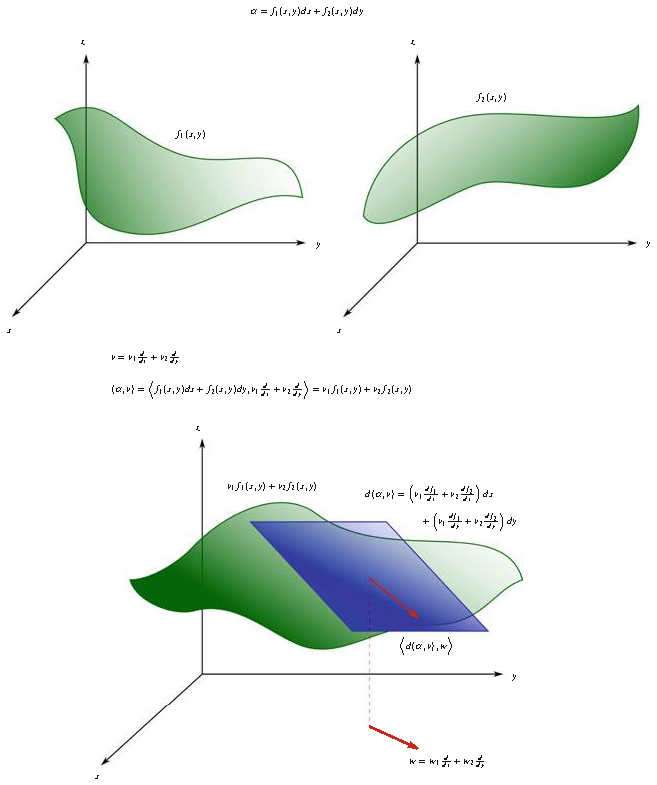
\includegraphics[width=0.960\linewidth]{images/vector/fig-4-1.pdf}
  \caption{流形 $\mathbb{R}^2$ 上的 1-形式 $\alpha(x,y)=f_1(x,y)dx+f_2(x,y)dy$ 由上面所示的两个函数 $f_1,f_2:\mathbb{R}^2\to\mathbb{R}$ 构成. 一旦我们给定流形 $\mathbb{R}^2$ 上的向量场 $v$（这里是常向量场 $v=v_1\partial_x+v_2\partial_y$）, 就可以用它求出实值函数 $\langle\alpha,v\rangle=v_1f_1+v_2f_2$, 它可以被看作两个函数 $f_1,f_2$ 的线性组合. 然后可以求这个函数在另一个给定向量 $w=w_1\partial_x+w_2\partial_y$ 方向上的方向导数. 这里微分 $d\langle\alpha,v\rangle$ 本质上编码了函数 $\langle\alpha,v\rangle$（以绿色显示）的切平面信息}
  \label{fig:4-1}
\end{figure}

总而言之, 我们这里有的
\[
d\langle\alpha,v\rangle(w)=v_1w_1\frac{\partial f_1}{\partial x}+v_2w_1\frac{\partial f_2}{\partial x}
+v_1w_2\frac{\partial f_1}{\partial y}+v_2w_2\frac{\partial f_2}{\partial y}
\]
是从流形 $\mathbb{R}^2$ 到 $\mathbb{R}$ 的函数. 当我们输入某个点 $p=(x_0,y_0)$ 时, 我们得到
\[
\begin{aligned}
d\langle\alpha_{(x_0,y_0)},v\rangle(w)
&=v_1w_1\left.\frac{\partial f_1(x,y)}{\partial x}\right|_{(x_0,y_0)}
+v_2w_1\left.\frac{\partial f_2(x,y)}{\partial x}\right|_{(x_0,y_0)}\\
&\qquad+v_1w_2\left.\frac{\partial f_1(x,y)}{\partial y}\right|_{(x_0,y_0)}
+v_2w_2\left.\frac{\partial f_2(x,y)}{\partial y}\right|_{(x_0,y_0)},
\end{aligned}
\]
这是一个数, 度量函数 $\langle\alpha,v\rangle=v_1f_1+v_2f_2$ 在给定点 $p=(x_0,y_0)$ 处沿向量 $w$ 移动时变化了多少.

这显然并不仅仅是度量 1-形式 $\alpha$ 如何变化. 相反, 它需要两个额外的向量 $v$ 和 $w$. 第一个向量 $v$ 与 1-形式一起用来构成实值函数 $\langle\alpha,v\rangle$, 然后用第二个向量来求这个函数的方向导数. 虽然这看起来是一种有点奇怪的度量 $\alpha$ 如何变化的方式, 但考虑到 1-形式作为一种数学对象实际上有多复杂, 这也许是我们能期望得到的最直截了当的方式了.

但在我们试图用这个公式以某种方式定义 1-形式 $\alpha$ 的微分之前, 我们决定谨慎一些, 看看当交换向量 $v$ 和 $w$ 的顺序时会发生什么. 也就是说, 我们想知道 $d\langle\alpha,w\rangle(v)$ 是什么. 毕竟, 如果我们简单地交换向量 $v$ 和 $w$ 的顺序, 我们会希望结果在某种意义上"相同". 继续这样做, 我们有 $\langle\alpha,w\rangle=w_1f_1+w_2f_2$, 这给出
\[
d\langle\alpha,w\rangle=\left(w_1\frac{\partial f_1}{\partial x}+w_2\frac{\partial f_2}{\partial x}\right)dx
+\left(w_1\frac{\partial f_1}{\partial y}+w_2\frac{\partial f_2}{\partial y}\right)dy,
\]
从而得到
\begin{align*}
d\langle\alpha,w\rangle(v)&=\bigl\langle d\langle\alpha,w\rangle,v\bigr\rangle\\
&=v_1w_1\frac{\partial f_1}{\partial x}+v_1w_2\frac{\partial f_2}{\partial x}
+v_2w_1\frac{\partial f_1}{\partial y}+v_2w_2\frac{\partial f_2}{\partial y}.
\end{align*}
让我们把这两个公式并排放在一起, 看看它们如何匹配.
\begin{align*}
\bigl\langle d\langle\alpha,v\rangle,w\bigr\rangle
&=v_1w_1\frac{\partial f_1}{\partial x}+v_2w_1\frac{\partial f_2}{\partial x}
+v_1w_2\frac{\partial f_1}{\partial y}+v_2w_2\frac{\partial f_2}{\partial y}\\
\bigl\langle d\langle\alpha,w\rangle,v\bigr\rangle
&=v_1w_1\frac{\partial f_1}{\partial x}+v_1w_2\frac{\partial f_2}{\partial x}
+v_2w_1\frac{\partial f_1}{\partial y}+v_2w_2\frac{\partial f_2}{\partial y}.
\end{align*}
所以, 这两个等式并不像我们可能希望的那样相同. 它们也不仅仅相差一个符号. 但显然 $d\langle\alpha,v\rangle(w)$ 与 $d\langle\alpha,w\rangle(v)$ 之间存在关系. 它们之间的关系要稍微复杂一些. 每个等式的第一项和最后一项是相同的, 但中间两项不同. 这两个公式都不能作为 1-形式导数的定义. 然而, 一切并没有失去. 一点巧妙的思考也许还能挽救局面.

在过去我们曾发现, 平行六面体的"体积"带有一个符号, 这个符号取决于向量的定向, 或者说顺序. 这种符号"歧义"已经出现在行列式的定义中, 然后出现在楔积的定义中. 因此, 如果我们最终确定的某种形式的导数的定义中出现这种符号, 我们也许不应过于惊讶或担心. 所以我们将使用一个在数学中时不时出现的"小技巧". 如果取这两项之差作为外微分的定义, 会发生什么？也就是说, 假设我们通过下面的公式定义 $\alpha$ 的外导数 $d\alpha$: 
\[
d\alpha(v,w)=\bigl\langle d\langle\alpha,w\rangle,v\bigr\rangle-\bigl\langle d\langle\alpha,v\rangle,w\bigr\rangle.
\]
用这个公式我们随后注意到, 交换 $v$ 和 $w$ 的顺序会改变符号, 
\begin{align*}
d\alpha(w,v)&=\bigl\langle d\langle\alpha,v\rangle,w\bigr\rangle-\bigl\langle d\langle\alpha,w\rangle,v\bigr\rangle\\
&=-\left(\bigl\langle d\langle\alpha,w\rangle,v\bigr\rangle-\bigl\langle d\langle\alpha,v\rangle,w\bigr\rangle\right)\\
&=-d\alpha(v,w).
\end{align*}
通过这样做, 我们得到 $d\alpha(v,w)$ 与 $d\alpha(w,v)$ 在相差一个符号的意义下给出相同的结果, 这是我们已经完全习惯并感到舒服的事情. 事实上, 考虑到符号在这个主题中的表现方式, 交换两个向量的顺序不改变某个东西的符号反而会令人惊讶. 所以, 我们将确定
\[
d\alpha(v,w)=\bigl\langle d\langle\alpha,w\rangle,v\bigr\rangle-\bigl\langle d\langle\alpha,v\rangle,w\bigr\rangle
\]
作为 $\alpha$ 的导数的工作定义. （实际上, 这个工作定义只在 $v$ 和 $w$ 恰好是常向量场时才有效, 但关于这一点我们稍后再说.）从几何上看, $d\alpha(v,w)$ 度量函数 $\langle\alpha,w\rangle$ 在 $v$ 方向上的变化减去函数 $\langle\alpha,v\rangle$ 在 $w$ 方向上的变化. 我们试图在图~\ref{fig:4-2} 中说明这一点.

\begin{figure}[htbp]
  \centering
  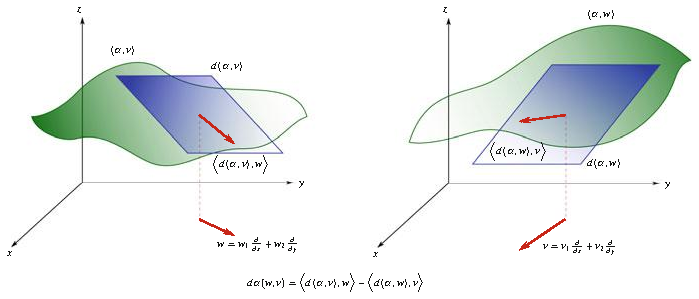
\includegraphics[width=0.960\linewidth]{images/vector/fig-4-2.pdf}
  \caption{左侧显示 $\langle\alpha,v\rangle$ 在 $w$ 方向上的变化, 右侧显示 $\langle\alpha,w\rangle$ 在 $v$ 方向上的变化. 这两个值之差随后被用来定义 $d\alpha(w,v)$. 这是度量 $\alpha$ 如何变化的一种间接方式}
  \label{fig:4-2}
\end{figure}

花点时间想想我们所做的. 由于 1-形式 $\alpha=f_1\,dx+f_2\,dy$ 是一个相当复杂的数学对象, 没有明显直接的方法度量它如何变化. 因此我们决定尝试用我们已经熟悉的技术, 即方向导数, 来间接度量 $\alpha$ 如何变化. 为了做到这一点, 我们需要两个（常）向量场 $v$ 和 $w$. 于是, 一旦我们给定了一个特定的 $v$ 和 $w$, 我们就用它们来间接度量 $\alpha$ 如何变化.

让我们用这个来得到 $d\alpha(v,w)$ 的实际表达式, 
\begin{align*}
d\alpha(v,w)&=\bigl\langle d\langle\alpha,w\rangle,v\bigr\rangle-\bigl\langle d\langle\alpha,v\rangle,w\bigr\rangle\\
&=v_1w_1\frac{\partial f_1}{\partial x}+v_1w_2\frac{\partial f_2}{\partial x}
+v_2w_1\frac{\partial f_1}{\partial y}+v_2w_2\frac{\partial f_2}{\partial y}\\
&\qquad-v_1w_1\frac{\partial f_1}{\partial x}-v_2w_1\frac{\partial f_2}{\partial x}
-v_1w_2\frac{\partial f_1}{\partial y}-v_2w_2\frac{\partial f_2}{\partial y}\\
&=v_1w_2\frac{\partial f_2}{\partial x}-v_1w_2\frac{\partial f_1}{\partial y}
-v_2w_1\frac{\partial f_2}{\partial x}+v_2w_1\frac{\partial f_1}{\partial y}\\
&=\left(\frac{\partial f_2}{\partial x}-\frac{\partial f_1}{\partial y}\right)(v_1w_2-w_1v_2)\\
&=\left(\frac{\partial f_2}{\partial x}-\frac{\partial f_1}{\partial y}\right)
\begin{vmatrix}v_1&w_1\\v_2&w_2\end{vmatrix}\\
&=\left(\frac{\partial f_2}{\partial x}-\frac{\partial f_1}{\partial y}\right)
\begin{vmatrix}dx(v)&dx(w)\\dy(v)&dy(w)\end{vmatrix}\\
&=\left(\frac{\partial f_2}{\partial x}-\frac{\partial f_1}{\partial y}\right)dx\wedge dy(v,w)\\
&=\left(\frac{\partial f_1}{\partial x}\underbrace{dx\wedge dx}_{=0}
+\frac{\partial f_1}{\partial y}\underbrace{dy\wedge dx}_{=-dx\wedge dy}
+\frac{\partial f_2}{\partial x}dx\wedge dy
+\frac{\partial f_2}{\partial y}\underbrace{dy\wedge dy}_{=0}\right)(v,w)\\
&=\Bigl(\underbrace{\left(\frac{\partial f_1}{\partial x}dx+\frac{\partial f_1}{\partial y}dy\right)}_{df_1}\wedge dx
+\underbrace{\left(\frac{\partial f_2}{\partial x}dx+\frac{\partial f_2}{\partial y}dy\right)}_{df_2}\wedge dy\Bigr)(v,w)\\
&=\bigl(df_1\wedge dx+df_2\wedge dy\bigr)(v,w).
\end{align*}
于是, 我们关于 $d\alpha$ 的"几何"定义——即函数 $\langle\alpha,w\rangle$ 在 $v$ 方向上的变化减去函数 $\langle\alpha,v\rangle$ 在 $w$ 方向上的变化——引导我们一路回到我们最初关于 $d\alpha$ 的公式 $\sum df_i\wedge dx_i$（当 $\alpha=\sum f_i\,dx_i$ 时）. 此外, 我们还有一个绝妙的额外收获: $d\alpha$ 结果是一个 2-形式. 好吧, 实际上这不仅仅是一个"额外收获". 这个定义导致 $d\alpha$ 是 2-形式这一事实, 正是我们确定这个（诚然有点笨拙的）1-形式外微分几何意义的首要原因.

实际上, 为了保持计算和图片的简单, 我们考察了流形 $\mathbb{R}^2$ 上的 1-形式 $\alpha$, 但我们本可以在任何流形上完成整个分析, 并得到同样的公式；只是计算会更麻烦一些.

我们意识到我们倾向于在不同记号之间跳来跳去, 而且我们将继续这样做. 我们实际上是故意这样做的, 让你习惯所有这些不同的记号很重要. 不同的书、论文和作者都倾向于使用不同的记号. 回顾 $df(v)=v[f]$ 以及 $\bigl\langle d\langle\alpha,w\rangle,v\bigr\rangle=v[\langle\alpha,w\rangle]$. 另外, 我们有 $\langle\alpha,w\rangle=\alpha(w)$, 所以我们可以把 $\bigl\langle d\langle\alpha,w\rangle,v\bigr\rangle$ 写成 $v[\alpha(w)]$. 类似地, 我们有 $\bigl\langle d\langle\alpha,v\rangle,w\bigr\rangle=w[\alpha(v)]$, 所以我们也可以把 $\alpha$ 的外导数（$v$ 和 $w$ 是常向量场）的定义写成
\begin{center}
\fbox{\parbox{0.86\textwidth}{\centering
\textbf{1-形式外微分的整体公式（常向量场）}\\[2pt]
$d\alpha(v,w)=\bigl\langle d\langle\alpha,w\rangle,v\bigr\rangle-\bigl\langle d\langle\alpha,v\rangle,w\bigr\rangle$
}}
\end{center}
或写成
\begin{center}
\fbox{\parbox{0.86\textwidth}{\centering
\textbf{1-形式外微分的整体公式（常向量场）}\\[2pt]
$d\alpha(v,w)=v[\alpha(w)]-w[\alpha(v)]$
}}
\end{center}

注意, 这正是我们在概述一节中给出的整体公式的前两项, 
\[
d\alpha(v,w)=v[\alpha(w)]-w[\alpha(v)]-\alpha([v,w]).
\]
于是我们看到, $d\alpha$ 的"几何"定义与 $d\alpha$ 的整体公式联系在一起. 然而, 我们缺少整体公式中的最后一项 $\alpha([v,w])$. 当 $v$ 和 $w$ 都是常向量场时这一项为零. 避开这一项的麻烦正是我们选择常向量场 $v$ 和 $w$ 的原因. 我们再次指出, 在这个整体公式中, 我们正在使用的实际坐标完全不出现. 这有时被称为坐标无关公式.

现在我们将对一个一般的 $n$ 维流形上的一般 1-形式快速重复这一过程. 这些计算适用于所谓的一般流形的坐标片. 这是我们将在后面某一章引入的概念, 所以现在只需想象我们在流形 $\mathbb{R}^n$ 上. 考虑 1-形式和向量
\[
\alpha=\sum_i\alpha_i\,dx_i,\qquad
v=\sum_i v_i\,\partial_{x_i},\qquad
w=\sum_i w_i\,\partial_{x_i}.
\]
于是我们有
\begin{align*}
\alpha(v)&=\langle\alpha,v\rangle\\
&=\left(\sum_i\alpha_i\,dx_i\right)\left(\sum_i v_i\,\partial_{x_i}\right)\\
&=\sum_i v_i\alpha_i.
\end{align*}
和以前一样, $\langle\alpha,v\rangle=\sum_i v_i\alpha_i$ 可以看作流形上的函数. 基本上, 这个函数是函数 $\alpha_i$ 以 $v_i$ 为权重的加权和. 使用在函数方向导数情形中定义的 $d$, 我们有
\begin{align*}
d\langle\alpha,v\rangle&=\sum_j\frac{\partial\left(\sum_i v_i\alpha_i\right)}{\partial x_j}dx_j\\
&=\sum_j\sum_i v_i\frac{\partial\alpha_i}{\partial x_j}dx_j.
\end{align*}
所以函数 $\langle\alpha,v\rangle=\sum_i v_i\alpha_i$ 在方向 $w$ 上的方向导数由下式给出
\begin{align*}
d\langle\alpha,v\rangle(w)&=\left(\sum_j\sum_i v_i\frac{\partial\alpha_i}{\partial x_j}dx_j\right)\left(\sum_k w_k\,\partial_{x_k}\right)\\
&=\sum_j\sum_i v_i\,w_j\frac{\partial\alpha_i}{\partial x_j}.
\end{align*}
回顾, 基本上 $d\langle\alpha,v\rangle$ 编码了函数 $\langle\alpha,v\rangle$ 的切空间, 而 $d\langle\alpha,v\rangle(w)$ 告诉我们沿 $w$ 移动时发生的变化. 一个完全相同的计算给出
\[
d\langle\alpha,w\rangle(v)=\sum_j\sum_i v_j\,w_i\frac{\partial\alpha_i}{\partial x_j}.
\]
比较 $d\langle\alpha,v\rangle(w)$ 和 $d\langle\alpha,w\rangle(v)$, 我们可以看到当 $i\neq j$ 时各项不同, 所以像以前一样, 我们定义
\begin{align*}
d\alpha(v,w)&=\bigl\langle d\langle\alpha,w\rangle,v\bigr\rangle-\bigl\langle d\langle\alpha,v\rangle,w\bigr\rangle\\
&=\sum_j\sum_i v_j\,w_i\frac{\partial\alpha_i}{\partial x_j}
-\sum_j\sum_i v_i\,w_j\frac{\partial\alpha_i}{\partial x_j}\\
&=\sum_j\sum_i\bigl(v_j\,w_i-v_i\,w_j\bigr)\frac{\partial\alpha_i}{\partial x_j}\\
&=\sum_j\sum_i\frac{\partial\alpha_i}{\partial x_j}
\begin{vmatrix}v_j&w_j\\v_i&w_i\end{vmatrix}\\
&=\sum_j\sum_i\frac{\partial\alpha_i}{\partial x_j}
\begin{vmatrix}dx_j(v)&dx_j(w)\\dx_i(v)&dx_i(w)\end{vmatrix}\\
&=\sum_j\sum_i\frac{\partial\alpha_i}{\partial x_j}dx_j\wedge dx_i\,(v,w)\\
&=\sum_i\left(\sum_j\frac{\partial\alpha_i}{\partial x_j}dx_j\right)\wedge dx_i\,(v,w)\\
&=\sum_i\underbrace{\left(\sum_j\frac{\partial\alpha_i}{\partial x_j}dx_j\right)}_{=d\alpha_i}\wedge dx_i\,(v,w).
\end{align*}
于是我们得到坐标内公式
\[
d\alpha=\sum_i d\alpha_i\wedge dx_i,
\]
这当然正是我们以前得到的.

与 1-形式的情形一样, 我们可以尝试为 $k$-形式 $\omega$ 的整体公式做一个几何论证. 第一步完全类似. 为了使用函数方向导数的概念, 我们必须通过放入不止一个而是 $k$ 个向量 $v_0,\ldots,v_{k-1}$ 把 $k$-形式变成一个函数, 然后我们度量这个函数在另一个向量 $v_k$ 方向上的变化. 然而, 下一步, 即我们实际使用数学"技巧"来定义 $d\omega$ 的那一步, 将很难合理化. 我们最终会得到
\begin{center}
\fbox{\parbox{0.86\textwidth}{\centering
\textbf{$k$-形式外微分的整体公式（常向量场）}\\[2pt]
$d\omega(v_0,\ldots,v_k)=\sum_i(-1)^i\bigl\langle d\bigl\langle\omega,(v_0,\ldots,\widehat{v_i},\ldots,v_k)\bigr\rangle,v_i\bigr\rangle$
}}
\end{center}
它也可以写成
\begin{center}
\fbox{\parbox{0.86\textwidth}{\centering
\textbf{$k$-形式外微分的整体公式（常向量场）}\\[2pt]
$d\omega(v_0,\ldots,v_k)=\sum_i(-1)^i\,v_i\bigl[\omega(v_0,\ldots,\widehat{v_i},\ldots,v_k)\bigr]$
}}
\end{center}
使用这个整体公式来得到坐标内公式也将是一个非常耗计算的过程. 因此我们将跳过它. 然而, 注意上面的公式与概述中的整体公式不同. 和以前一样, 这是因为我们使用的是常向量场.

\subsection{非常值向量场情形下的外微分}

我们对常向量场 $v$ 和 $w$ 所做的, 是作一些几何论证, 说明 $d\alpha(v,w)=v[\alpha(w)]-w[\alpha(v)]$ 会是用作 $\alpha$ 外微分整体公式的好定义. 然后我们用这个公式求出 1-形式 $\alpha=\sum_i\alpha_i\,dx_i$ 的外微分的坐标内公式, 发现它是 $d\alpha=\sum_i d\alpha_i\wedge dx_i$. 我们现在假设这就是我们想要的一般整体公式的坐标内形式.

由于我们并不是要给出外微分整体公式的实际证明, 而只是想让你对公式为什么是这样的以及如何成为这样的有一个感觉, 所以我们不会尝试逻辑上严谨的论证. 我们即将要做的实际上在逻辑上是反过来的. 我们知道我们想要得到的答案, 也就是说, 我们知道外导数的坐标内公式应该是什么, 所以我们将实际利用我们想最终到达哪里的知识, 来帮助我们找到并理解外微分的一般整体公式. 外微分的一般整体公式实际上将在第 A.7 节中以完全不同的方式证明, 使用附录中引入的许多概念和恒等式. 那节中的证明非常计算化, 公式似乎奇迹般地从各种配料的混合中冒出来. 本节则更脚踏实地, 给出动机, 并在更大程度上处理潜在的几何.

我们从 $\mathbb{R}^2$ 上的 1-形式 $\alpha$ 和两个非常值向量场 $v$、$w$ 开始, 
\[
\alpha=f_1\,dx+f_2\,dy,\qquad
v=g_1\,\partial_x+g_2\,\partial_y=\binom{g_1}{g_2},\qquad
w=h_1\,\partial_x+h_2\,\partial_y=\binom{h_1}{h_2},
\]
其中 $f_1,f_2,g_1,g_2,h_1,h_2$ 是流形 $\mathbb{R}^2$ 上的实值函数.

正如我们所说, 我们将从我们知道想得到的答案开始. 我们想要的 $\alpha$ 的外微分的坐标内公式是 $d\alpha=\sum_i d\alpha_i\wedge dx_i$. 所以我们首先计算它, 
\begin{align*}
d\alpha&=df_1\wedge dx+df_2\wedge dy\\
&=\left(\frac{\partial f_1}{\partial x}dx+\frac{\partial f_1}{\partial y}dy\right)\wedge dx
+\left(\frac{\partial f_2}{\partial x}dx+\frac{\partial f_2}{\partial y}dy\right)\wedge dy\\
&=\frac{\partial f_1}{\partial x}\underbrace{dx\wedge dx}_{=0}+\frac{\partial f_1}{\partial y}\underbrace{dy\wedge dx}_{=-dx\wedge dy}
+\frac{\partial f_2}{\partial x}dx\wedge dy+\frac{\partial f_2}{\partial y}\underbrace{dy\wedge dy}_{=0}\\
&=\left(\frac{\partial f_2}{\partial x}-\frac{\partial f_1}{\partial y}\right)dx\wedge dy.
\end{align*}
把我们的向量场 $v$ 和 $w$ 代进去, 我们得到
\begin{align*}
d\alpha(v,w)&=\left(\frac{\partial f_2}{\partial x}-\frac{\partial f_1}{\partial y}\right)dx\wedge dy(v,w)\\
&=\left(\frac{\partial f_2}{\partial x}-\frac{\partial f_1}{\partial y}\right)
\begin{vmatrix}dx(v)&dx(w)\\dy(v)&dy(w)\end{vmatrix}\\
&=\left(\frac{\partial f_2}{\partial x}-\frac{\partial f_1}{\partial y}\right)
\begin{vmatrix}g_1&h_1\\g_2&h_2\end{vmatrix}\\
&=\left(\frac{\partial f_2}{\partial x}-\frac{\partial f_1}{\partial y}\right)(g_1h_2-g_2h_1)\\
&=g_1h_2\frac{\partial f_2}{\partial x}-g_1h_2\frac{\partial f_1}{\partial y}
-g_2h_1\frac{\partial f_2}{\partial x}+g_2h_1\frac{\partial f_1}{\partial y}.
\end{align*}
到现在为止我们应该对这类计算感到舒服了. 唯一的区别是常数 $v_1,v_2,w_1,w_2$ 被函数 $g_1,g_2,h_1,h_2$ 取代了. 这就是我们想得到的答案. 稍后我们将回过头来参考这个等式.

我们的策略与常向量场情形相同, 出于同样的几何原因. 事实上, 基于常向量场情形, 我们首先猜想整体公式是 $d\alpha(v,w)=v[\alpha(w)]-w[\alpha(v)]$. 我们将做这个（诚然很乱的）计算, 发现它的项比上面求出的 $d\alpha(v,w)$ 的局部公式多得多. 然后我们将把这些项归并在一起, 并把它们称为 $\alpha([v,w])$, 从而对 1-形式的情形给出完整的整体公式 $d\alpha(v,w)=v[\alpha(w)]-w[\alpha(v)]-\alpha([v,w])$. 当然, 在那个时候你还不知道 $\alpha([v,w])$ 是什么. 然后我们将花一些时间解释这最后一项实际上表示什么. 括号 $[\,\cdot\,,\cdot\,]$（其中点被向量取代）被称为李括号, 所以 $[v,w]$ 是 $v$ 和 $w$ 的李括号, 结果它也是另一个向量场, 这很好, 因为它要被 1-形式 $\alpha$ 吞入.

现在我们准备开始了. 同样的论证适用. 我们想以某种方式度量 $\alpha$ 如何变化. 由于我们不确定如何做到这一点, 我们先把 $\alpha$ 变成我们知道如何研究的东西, 即一个函数, 这可以通过把它与向量场 $v$（它不再需要是常向量场）配对来完成, 
\[
\langle\alpha,v\rangle=[f_1,f_2]\binom{g_1}{g_2}=f_1g_1+f_2g_2.
\]
把这个与常向量场的情形相比较, 在那种情形中我们得到 $v_1f_1+v_2f_2$, 其中 $v_1$ 和 $v_2$ 是常数. 现在的情况立即更复杂了, 因为它涉及函数的乘积, 而不仅仅是函数的加权和.

为了求函数 $f_1g_1+f_2g_2$ 的方向导数, 我们首先求函数 $\langle\alpha,v\rangle$ 的微分, 
\begin{align*}
d\langle\alpha,v\rangle&=\frac{\partial(f_1g_1+f_2g_2)}{\partial x}dx+\frac{\partial(f_1g_1+f_2g_2)}{\partial y}dy\\
&=\left(\frac{\partial(f_1g_1)}{\partial x}+\frac{\partial(f_2g_2)}{\partial x}\right)dx
+\left(\frac{\partial(f_1g_1)}{\partial y}+\frac{\partial(f_2g_2)}{\partial y}\right)dy\\
&=\left(\frac{\partial f_1}{\partial x}\cdot g_1+f_1\cdot\frac{\partial g_1}{\partial x}
+\frac{\partial f_2}{\partial x}\cdot g_2+f_2\cdot\frac{\partial g_2}{\partial x}\right)dx\\
&\qquad+\left(\frac{\partial f_1}{\partial y}\cdot g_1+f_1\cdot\frac{\partial g_1}{\partial y}
+\frac{\partial f_2}{\partial y}\cdot g_2+f_2\cdot\frac{\partial g_2}{\partial y}\right)dy.
\end{align*}
注意, 这里需要使用乘积法则, 导致项的数目是我们以前处理常向量场时的两倍. 而且这些项本身也是函数的乘积. 这就是处理非常值向量场复杂得多的原因. 我们现在通过
\begin{align*}
\bigl\langle d\langle\alpha,v\rangle,w\bigr\rangle
&=\left(\frac{\partial f_1}{\partial x}\cdot g_1+f_1\cdot\frac{\partial g_1}{\partial x}
+\frac{\partial f_2}{\partial x}\cdot g_2+f_2\cdot\frac{\partial g_2}{\partial x}\right)h_1\\
&\qquad+\left(\frac{\partial f_1}{\partial y}\cdot g_1+f_1\cdot\frac{\partial g_1}{\partial y}
+\frac{\partial f_2}{\partial y}\cdot g_2+f_2\cdot\frac{\partial g_2}{\partial y}\right)h_2\\
&=g_1h_1\frac{\partial f_1}{\partial x}+f_1h_1\frac{\partial g_1}{\partial x}
+g_2h_1\frac{\partial f_2}{\partial x}+f_2h_1\frac{\partial g_2}{\partial x}\\
&\qquad+g_1h_2\frac{\partial f_1}{\partial y}+f_1h_2\frac{\partial g_1}{\partial y}
+g_2h_2\frac{\partial f_2}{\partial y}+f_2h_2\frac{\partial g_2}{\partial y}
\end{align*}
来求 $\langle\alpha,v\rangle$ 在 $w$ 方向上的方向导数.

接下来我们交换向量场 $v$ 和 $w$ 重复这个过程, 
\[
\langle\alpha,w\rangle=[f_1,f_2]\binom{h_1}{h_2}=f_1h_1+f_2h_2.
\]
为了求方向导数, 我们需要
\begin{align*}
d\langle\alpha,w\rangle&=\frac{\partial(f_1h_1+f_2h_2)}{\partial x}dx+\frac{\partial(f_1h_1+f_2h_2)}{\partial y}dy\\
&=\left(\frac{\partial(f_1h_1)}{\partial x}+\frac{\partial(f_2h_2)}{\partial x}\right)dx
+\left(\frac{\partial(f_1h_1)}{\partial y}+\frac{\partial(f_2h_2)}{\partial y}\right)dy\\
&=\left(\frac{\partial f_1}{\partial x}\cdot h_1+f_1\cdot\frac{\partial h_1}{\partial x}
+\frac{\partial f_2}{\partial x}\cdot h_2+f_2\cdot\frac{\partial h_2}{\partial x}\right)dx\\
&\qquad+\left(\frac{\partial f_1}{\partial y}\cdot h_1+f_1\cdot\frac{\partial h_1}{\partial y}
+\frac{\partial f_2}{\partial y}\cdot h_2+f_2\cdot\frac{\partial h_2}{\partial y}\right)dy.
\end{align*}
于是 $\langle\alpha,w\rangle$ 在 $v$ 方向上的方向导数由下式给出
\begin{align*}
\bigl\langle d\langle\alpha,w\rangle,v\bigr\rangle
&=\left(\frac{\partial f_1}{\partial x}\cdot h_1+f_1\cdot\frac{\partial h_1}{\partial x}
+\frac{\partial f_2}{\partial x}\cdot h_2+f_2\cdot\frac{\partial h_2}{\partial x}\right)g_1\\
&\qquad+\left(\frac{\partial f_1}{\partial y}\cdot h_1+f_1\cdot\frac{\partial h_1}{\partial y}
+\frac{\partial f_2}{\partial y}\cdot h_2+f_2\cdot\frac{\partial h_2}{\partial y}\right)g_2\\
&=h_1g_1\frac{\partial f_1}{\partial x}+f_1g_1\frac{\partial h_1}{\partial x}
+h_2g_1\frac{\partial f_2}{\partial x}+f_2g_1\frac{\partial h_2}{\partial x}\\
&\qquad+h_1g_2\frac{\partial f_1}{\partial y}+f_1g_2\frac{\partial h_1}{\partial y}
+h_2g_2\frac{\partial f_2}{\partial y}+f_2g_2\frac{\partial h_2}{\partial y}.
\end{align*}

回顾在我们的策略中, 我们首先猜想 $d\alpha(v,w)=v[\alpha(w)]-w[\alpha(v)]$. 在常向量情形中我们选择它, 仅仅因为它似乎是可行的, 而且它还导致交换向量 $v$ 和 $w$ 会改变符号这一事实. 按照我们的假设进行下去, 我们有
\begin{align*}
d\alpha(v,w)&=v[\alpha(w)]-w[\alpha(v)]\\
&\overset{\text{假设}}{=}\bigl\langle d\langle\alpha,w\rangle,v\bigr\rangle-\bigl\langle d\langle\alpha,v\rangle,w\bigr\rangle\\
&=h_1g_1\frac{\partial f_1}{\partial x}+f_1g_1\frac{\partial h_1}{\partial x}
+h_2g_1\frac{\partial f_2}{\partial x}+f_2g_1\frac{\partial h_2}{\partial x}
+h_1g_2\frac{\partial f_1}{\partial y}+f_1g_2\frac{\partial h_1}{\partial y}\\
&\qquad+h_2g_2\frac{\partial f_2}{\partial y}+f_2g_2\frac{\partial h_2}{\partial y}\\
&\qquad-g_1h_1\frac{\partial f_1}{\partial x}-f_1h_1\frac{\partial g_1}{\partial x}
-g_2h_1\frac{\partial f_2}{\partial x}-f_2h_1\frac{\partial g_2}{\partial x}
-g_1h_2\frac{\partial f_1}{\partial y}-f_1h_2\frac{\partial g_1}{\partial y}\\
&\qquad-g_2h_2\frac{\partial f_2}{\partial y}-f_2h_2\frac{\partial g_2}{\partial y}.
\end{align*}
注意, 有四项立刻消掉了. 由于我们已经知道我们想要的局部坐标内公式看起来是什么样, 现在我们转向它. 基于上面的计算, 我们试图到达的是
\[
d\alpha(v,w)=g_1h_2\frac{\partial f_2}{\partial x}-g_1h_2\frac{\partial f_1}{\partial y}
-g_2h_1\frac{\partial f_2}{\partial x}+g_2h_1\frac{\partial f_1}{\partial y}.
\]
因此我们有八个多余项
\[
f_1g_1\frac{\partial h_1}{\partial x}+f_2g_1\frac{\partial h_2}{\partial x}
+f_1g_2\frac{\partial h_1}{\partial y}+f_2g_2\frac{\partial h_2}{\partial y}
-f_1h_1\frac{\partial g_1}{\partial x}-f_2h_1\frac{\partial g_2}{\partial x}
-f_1h_2\frac{\partial g_1}{\partial y}-f_2h_2\frac{\partial g_2}{\partial y}.
\]
正如我们策略中所说的, 我们将把这些项归并在一起, 并把它们称为 $\alpha([v,w])$, 得到
\[
\begin{aligned}
\alpha([v,w])&=f_1g_1\frac{\partial h_1}{\partial x}+f_2g_1\frac{\partial h_2}{\partial x}
+f_1g_2\frac{\partial h_1}{\partial y}+f_2g_2\frac{\partial h_2}{\partial y}\\
&\qquad-f_1h_1\frac{\partial g_1}{\partial x}-f_2h_1\frac{\partial g_2}{\partial x}
-f_1h_2\frac{\partial g_1}{\partial y}-f_2h_2\frac{\partial g_2}{\partial y}.
\end{aligned}
\]
于是这反过来给出整体公式
\[
d\alpha(v,w)=v[\alpha(w)]-w[\alpha(v)]-\alpha([v,w]).
\]
当然, 在这一点上, 这个整体公式中的最后一项似乎只不过是一个记号上的方便；我们不知道它实际上表示什么. 事实是, 第三项确实表示某种几何上有趣而重要的东西, 我们现在就来解释.

两个向量场 $v$ 和 $w$ 的李括号的定义, 记为 $[v,w]$, 是根据这些向量场如何作用于函数 $F:\mathbb{R}^2\to\mathbb{R}$ 来定义的. 给定定义在流形 $\mathbb{R}^2$ 上的向量场 $w$, 我们可以求 $F$ 在 $w$ 方向上的方向导数. 在特定点 $p\in\mathbb{R}^2$ 处, $w_p[F]$ 是一个值, 告诉我们 $F$ 在点 $p$ 处沿 $w$ 方向变化有多快. 但如果我们不指定点 $p$, 那么 $w[F]$ 就是流形 $\mathbb{R}^2$ 上的另一个函数. 也就是说, 
\[
w[F]:\mathbb{R}^2\to\mathbb{R},\qquad p\longmapsto w_p[F].
\]
我们可以再次取这个函数 $w[F]$ 在 $v$ 方向上的方向导数. 同样, 在点 $p\in\mathbb{R}^2$ 处, $v_p[w[F]]$ 是一个值, 告诉我们 $w[F]$ 在点 $p$ 处沿 $v$ 方向变化有多快. 然而, 如果我们不指定点, 那么 $v[w[F]]$ 又是流形 $\mathbb{R}^2$ 上的另一个函数, 
\[
v[w[F]]:\mathbb{R}^2\to\mathbb{R},\qquad p\longmapsto v_p\bigl[w[F]\bigr].
\]

\begin{figure}[htbp]
  \centering
  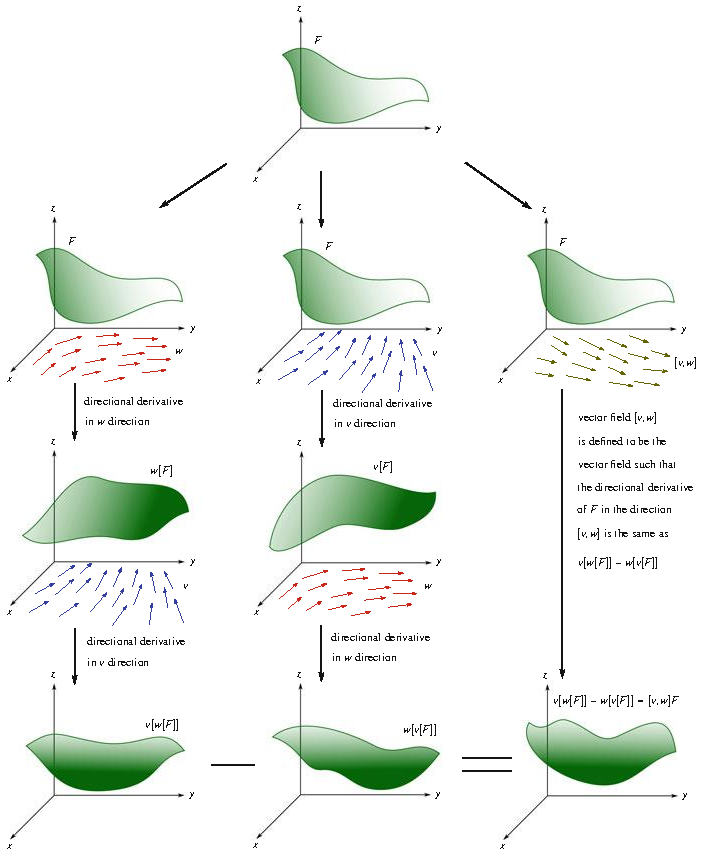
\includegraphics[width=0.960\linewidth]{images/vector/fig-4-3.pdf}
  \caption{在左侧, 我们取 $F:\mathbb{R}^2\to\mathbb{R}$ 在 $w$ 方向上的方向导数, 得到函数 $w[F]$, 然后再取 $w[F]$ 在 $v$ 方向上的方向导数, 得到函数 $v[w[F]]$. 在中间, 我们取 $F$ 在 $v$ 方向上的方向导数, 得到函数 $v[F]$, 然后再取 $v[F]$ 在 $w$ 方向上的方向导数, 得到 $w[v[F]]$. 取这两个函数之差 $v[w[F]]-w[v[F]]$, 得到一个新函数, 显示在底部. $v$ 和 $w$ 的李括号（记为 $[v,w]$）就是这样的向量场: 当应用于原始函数 $F$ 时, 它给出这个新函数. 换句话说, $[v,w]F=v[w[F]]-w[v[F]]$, 如右侧所示}
  \label{fig:4-3}
\end{figure}

这个过程全部在图~\ref{fig:4-3} 的左侧作了说明. 如果我们颠倒向量场的顺序, 先用 $v$, 我们得到函数 $v[F]:\mathbb{R}^2\to\mathbb{R}$. 接着应用 $w$, 我们得到函数 $w[v[F]]:\mathbb{R}^2\to\mathbb{R}$. 这个过程在图~\ref{fig:4-3} 的中部作了说明. 假设我们随后取这两个函数之差, 如图~\ref{fig:4-3} 的底部那样, 那么我们会得到一个新函数
\[
v\bigl[w[F]\bigr]-w\bigl[v[F]\bigr]:\mathbb{R}^2\to\mathbb{R}.
\]
事实上, 有可能找到一个单一的向量场, 一步完成这一切. 换句话说, 我们可以找到一个单一的向量场, 当应用于 $F$ 时恰好给出这个函数 $v[w[F]]-w[v[F]]$. 这个单一的向量场被称为 $v$ 和 $w$ 的李括号, 记为 $[v,w]$. 于是我们有
\[
[v,w]F=v\bigl[w[F]\bigr]-w\bigl[v[F]\bigr].
\]
这显示在图~\ref{fig:4-3} 的右侧. 尽管记号 $[v,w]$ 中包含两个向量场 $v$ 和 $w$, 但 $[v,w]$ 只是一个单一的向量场. 还要注意, 方括号有两种不同的用法. 然而, 通过注意方括号里面是什么, 应该很容易区分这两种用法. 我们将在下面用计算求出 $[v,w]$, 但应该指出, 还有一种看待 $[v,w]$ 的稍微几何化一点的方式. 事实上, 结果 $[v,w]$ 就是 $w$ 在 $v$ 方向上的李导数. 对这一点的解释留到第~\ref{sec:A-7} 节和图~\ref{fig:A-5}、\ref{fig:A-6}.

假设我们在记号中去掉函数 $F$, 得到
\[
[v,w]\,\cdot\,=v\bigl[w[\,\cdot\,]\bigr]-w\bigl[v[\,\cdot\,]\bigr].
\]
这解释了为什么你几乎总是会看到 $v$ 和 $w$ 的李括号被偷懒地定义为
\[
[v,w]=vw-wv.
\]

我们的目标现在转向确切找出向量场 $[v,w]$ 是什么, 
\begin{align*}
[v,w]F&=(vw-wv)F\\
&=v\bigl[w[F]\bigr]-w\bigl[v[F]\bigr]\\
&=v\left(h_1\frac{\partial F}{\partial x}+h_2\frac{\partial F}{\partial y}\right)
-w\left(g_1\frac{\partial F}{\partial x}+g_2\frac{\partial F}{\partial y}\right)\\
&=(g_1\partial_x+g_2\partial_y)\left(h_1\frac{\partial F}{\partial x}+h_2\frac{\partial F}{\partial y}\right)
-(h_1\partial_x+h_2\partial_y)\left(g_1\frac{\partial F}{\partial x}+g_2\frac{\partial F}{\partial y}\right)\\
&=g_1\frac{\partial}{\partial x}\left(h_1\frac{\partial F}{\partial x}\right)
+g_1\frac{\partial}{\partial x}\left(h_2\frac{\partial F}{\partial y}\right)
+g_2\frac{\partial}{\partial y}\left(h_1\frac{\partial F}{\partial x}\right)
+g_2\frac{\partial}{\partial y}\left(h_2\frac{\partial F}{\partial y}\right)\\
&\qquad-h_1\frac{\partial}{\partial x}\left(g_1\frac{\partial F}{\partial x}\right)
-h_1\frac{\partial}{\partial x}\left(g_2\frac{\partial F}{\partial y}\right)
-h_2\frac{\partial}{\partial y}\left(g_1\frac{\partial F}{\partial x}\right)
-h_2\frac{\partial}{\partial y}\left(g_2\frac{\partial F}{\partial y}\right)\\
&\overset{\text{积法则}}{=}g_1\frac{\partial h_1}{\partial x}\frac{\partial F}{\partial x}
+g_1h_1\frac{\partial^2 F}{\partial x^2}
+g_1\frac{\partial h_2}{\partial x}\frac{\partial F}{\partial y}
+g_1h_2\frac{\partial^2 F}{\partial x\partial y}\\
&\qquad+g_2\frac{\partial h_1}{\partial y}\frac{\partial F}{\partial x}
+g_2h_1\frac{\partial^2 F}{\partial y\partial x}
+g_2\frac{\partial h_2}{\partial y}\frac{\partial F}{\partial y}
+g_2h_2\frac{\partial^2 F}{\partial y^2}\\
&\qquad-h_1\frac{\partial g_1}{\partial x}\frac{\partial F}{\partial x}
-h_1g_1\frac{\partial^2 F}{\partial x^2}
-h_1\frac{\partial g_2}{\partial x}\frac{\partial F}{\partial y}
-h_1g_2\frac{\partial^2 F}{\partial x\partial y}\\
&\qquad-h_2\frac{\partial g_1}{\partial y}\frac{\partial F}{\partial x}
-h_2g_1\frac{\partial^2 F}{\partial y\partial x}
-h_2\frac{\partial g_2}{\partial y}\frac{\partial F}{\partial y}
-h_2g_2\frac{\partial^2 F}{\partial y^2}\\
&=g_1\frac{\partial h_1}{\partial x}\frac{\partial F}{\partial x}
+g_1\frac{\partial h_2}{\partial x}\frac{\partial F}{\partial y}
+g_2\frac{\partial h_1}{\partial y}\frac{\partial F}{\partial x}
+g_2\frac{\partial h_2}{\partial y}\frac{\partial F}{\partial y}\\
&\qquad-h_1\frac{\partial g_1}{\partial x}\frac{\partial F}{\partial x}
-h_1\frac{\partial g_2}{\partial x}\frac{\partial F}{\partial y}
-h_2\frac{\partial g_1}{\partial y}\frac{\partial F}{\partial x}
-h_2\frac{\partial g_2}{\partial y}\frac{\partial F}{\partial y}\\
&=\left(g_1\frac{\partial h_1}{\partial x}+g_2\frac{\partial h_1}{\partial y}
-h_1\frac{\partial g_1}{\partial x}-h_2\frac{\partial g_1}{\partial y}\right)\frac{\partial}{\partial x}[F]\\
&\qquad+\left(g_1\frac{\partial h_2}{\partial x}+g_2\frac{\partial h_2}{\partial y}
-h_1\frac{\partial g_2}{\partial x}-h_2\frac{\partial g_2}{\partial y}\right)\frac{\partial}{\partial y}[F]
\end{align*}
其中各项由于混合偏导数的相等而相消. 于是我们找到了向量场 $[v,w]$ 所取的形式, 它由下式给出
\[
[v,w]=\left(g_1\frac{\partial h_1}{\partial x}+g_2\frac{\partial h_1}{\partial y}
-h_1\frac{\partial g_1}{\partial x}-h_2\frac{\partial g_1}{\partial y}\right)\partial_x
+\left(g_1\frac{\partial h_2}{\partial x}+g_2\frac{\partial h_2}{\partial y}
-h_1\frac{\partial g_2}{\partial x}-h_2\frac{\partial g_2}{\partial y}\right)\partial_y
\]
即
\[
[v,w]=
\begin{bmatrix}
g_1\frac{\partial h_1}{\partial x}+g_2\frac{\partial h_1}{\partial y}-h_1\frac{\partial g_1}{\partial x}-h_2\frac{\partial g_1}{\partial y}\\[4pt]
g_1\frac{\partial h_2}{\partial x}+g_2\frac{\partial h_2}{\partial y}-h_1\frac{\partial g_2}{\partial x}-h_2\frac{\partial g_2}{\partial y}
\end{bmatrix}.
\]

现在让我们看看 $\alpha$ 作用于向量场 $[v,w]$ 是什么. 我们有
\begin{align*}
\alpha([v,w])&=\bigl\langle\alpha,[v,w]\bigr\rangle\\
&=[f_1,f_2]\begin{bmatrix}
g_1\frac{\partial h_1}{\partial x}+g_2\frac{\partial h_1}{\partial y}-h_1\frac{\partial g_1}{\partial x}-h_2\frac{\partial g_1}{\partial y}\\[4pt]
g_1\frac{\partial h_2}{\partial x}+g_2\frac{\partial h_2}{\partial y}-h_1\frac{\partial g_2}{\partial x}-h_2\frac{\partial g_2}{\partial y}
\end{bmatrix}\\
&=f_1g_1\frac{\partial h_1}{\partial x}+f_1g_2\frac{\partial h_1}{\partial y}
-f_1h_1\frac{\partial g_1}{\partial x}-f_1h_2\frac{\partial g_1}{\partial y}\\
&\qquad+f_2g_1\frac{\partial h_2}{\partial x}+f_2g_2\frac{\partial h_2}{\partial y}
-f_2h_1\frac{\partial g_2}{\partial x}-f_2h_2\frac{\partial g_2}{\partial y}.
\end{align*}
这里注意记号, $[v,w]$ 是两个向量场的李括号, 它本身是一个向量场, 而 $[f_1,f_2]$ 是与微分 1-形式 $\alpha=f_1\,dx+f_2\,dy$ 相联系的余向量, 即行向量. 区分这两个数学上不同的对象的方法是密切注意括号里面是什么: 向量场还是函数. 但注意我们得到的东西, 这八项正好就是 $v[\alpha(w)]-w[\alpha(v)]$ 中剩下的八项. 因此, 我们把流形 $\mathbb{R}^2$ 上 1-形式 $\alpha$ 的外微分的整体公式定义为
\[
d\alpha(v,w)=v[\alpha(w)]-w[\alpha(v)]-\alpha([v,w]).
\]

当然, 到目前为止我们只对流形 $\mathbb{R}^2$ 上的 1-形式做了这些. 流形 $\mathbb{R}^n$ 上的一般 1-形式又怎样呢？我们将同样走一遍这些（诚然相当复杂的）计算, 以确认一切都像预期的那样成立. 我们从
\[
\alpha=\sum_i\alpha_i\,dx_i,\qquad
v=\sum_i g_i\,\partial_{x_i},\qquad
w=\sum_i h_i\,\partial_{x_i}
\]
开始. 我们首先计算 $[v,w]$. 使用流形上的实值函数 $F$, 我们首先求出
\begin{align*}
v\bigl[w[F]\bigr]&=v\left(\sum_i h_i\frac{\partial F}{\partial x_i}\right)\\
&=\left(\sum_j g_j\,\partial_{x_j}\right)\left(\sum_i h_i\frac{\partial F}{\partial x_i}\right)\\
&=\sum_j g_j\,\partial_{x_j}\left(\sum_i h_i\frac{\partial F}{\partial x_i}\right)\\
&=\sum_j\sum_i g_j\left(\frac{\partial h_i}{\partial x_j}\cdot\frac{\partial F}{\partial x_i}
+h_i\frac{\partial}{\partial x_j}\left(\frac{\partial F}{\partial x_i}\right)\right)\\
&=\sum_j\sum_i\left(g_j\frac{\partial h_i}{\partial x_j}\cdot\frac{\partial F}{\partial x_i}
+g_jh_i\frac{\partial}{\partial x_j}\left(\frac{\partial F}{\partial x_i}\right)\right).
\end{align*}
求下一项是类似的, 我们得到
\[
w\bigl[v[F]\bigr]=\sum_j\sum_i\left(h_j\frac{\partial g_i}{\partial x_j}\cdot\frac{\partial F}{\partial x_i}
+h_jg_j\frac{\partial}{\partial x_j}\left(\frac{\partial F}{\partial x_i}\right)\right).
\]
把这两项放在一起, 我们得到
\begin{align*}
v\bigl[w[F]\bigr]-w\bigl[v[F]\bigr]
&=\sum_j\sum_i\left(g_j\frac{\partial h_i}{\partial x_j}\cdot\frac{\partial F}{\partial x_i}
+g_jh_i\frac{\partial}{\partial x_j}\left(\frac{\partial F}{\partial x_i}\right)\right)\\
&\qquad-\sum_j\sum_i\left(h_j\frac{\partial g_i}{\partial x_j}\cdot\frac{\partial F}{\partial x_i}
+h_jg_j\frac{\partial}{\partial x_j}\left(\frac{\partial F}{\partial x_i}\right)\right)\\
&=\sum_j\sum_i\left(g_j\frac{\partial h_i}{\partial x_j}-h_j\frac{\partial g_i}{\partial x_j}\right)\frac{\partial F}{\partial x_i}\\
&\qquad+\underbrace{\sum_i\sum_j g_jh_i\frac{\partial}{\partial x_j}\left(\frac{\partial F}{\partial x_i}\right)
-\sum_j\sum_i h_jg_j\frac{\partial}{\partial x_j}\left(\frac{\partial F}{\partial x_i}\right)}_{=0, \text{交换哑指标}}\\
&=\sum_i\left(\sum_j\left(g_j\frac{\partial h_i}{\partial x_j}-h_j\frac{\partial g_i}{\partial x_j}\right)\right)\frac{\partial F}{\partial x_i}.
\end{align*}
去掉函数 $F$ 我们得到实际的向量场
\[
[v,w]=\sum_i\left(\sum_j\left(g_j\frac{\partial h_i}{\partial x_j}-h_j\frac{\partial g_i}{\partial x_j}\right)\right)\partial_{x_i}.
\]
最后, 我们求出
\begin{align*}
\alpha([v,w])&=\left(\sum_k\alpha_k\,dx_k\right)
\left(\sum_i\left(\sum_j\left(g_j\frac{\partial h_i}{\partial x_j}-h_j\frac{\partial g_i}{\partial x_j}\right)\right)\partial_{x_i}\right)\\
&=\sum_i\alpha_i\left(\sum_j\left(g_j\frac{\partial h_i}{\partial x_j}-h_j\frac{\partial g_i}{\partial x_j}\right)\right).
\end{align*}
现在我们把注意力转向表达式 $v[\alpha(w)]-w[\alpha(v)]-\alpha([v,w])$. 由于
\[
v[\alpha(w)]=d(\alpha(v))(w)=\bigl\langle d(\alpha(v)),w\bigr\rangle
=\bigl\langle d\langle\alpha,v\rangle,w\bigr\rangle,
\]
我们从
\[
\langle\alpha,v\rangle=\left(\sum_i\alpha_i\,dx_i\right)\left(\sum_j g_j\,\partial_{x_j}\right)=\sum_i\alpha_i g_i
\]
开始. 求方向导数我们得到
\begin{align*}
d\langle\alpha,v\rangle&=d\left(\sum_i\alpha_i g_i\right)\\
&=\sum_j\frac{\partial\left(\sum_i\alpha_i g_i\right)}{\partial x_j}dx_j\\
&=\sum_j\sum_i\left(g_i\frac{\partial\alpha_i}{\partial x_j}+\alpha_i\frac{\partial g_i}{\partial x_j}\right)dx_j,
\end{align*}
然后用它求出
\[
w[\alpha(v)]=\sum_j\sum_i h_j\left(g_i\frac{\partial\alpha_i}{\partial x_j}+\alpha_i\frac{\partial g_i}{\partial x_j}\right).
\]
类似地我们有
\[
v[\alpha(w)]=\sum_j\sum_i g_j\left(h_i\frac{\partial\alpha_i}{\partial x_j}+\alpha_i\frac{\partial h_i}{\partial x_j}\right).
\]
接下来, 我们把一切组合起来
\begin{align*}
d\alpha(v,w)&=v[\alpha(w)]-w[\alpha(v)]-\alpha([v,w])\\
&=\sum_j\sum_i g_jh_i\frac{\partial\alpha_i}{\partial x_j}
+\sum_j\sum_i g_j\alpha_i\frac{\partial h_i}{\partial x_j}
-\sum_j\sum_i h_jg_i\frac{\partial\alpha_i}{\partial x_j}
-\sum_j\sum_i h_j\alpha_i\frac{\partial g_i}{\partial x_j}\\
&\qquad-\sum_i\alpha_i\sum_j\left(g_j\frac{\partial h_i}{\partial x_j}-h_j\frac{\partial g_i}{\partial x_j}\right)\\
&=\sum_{i,j}\bigl(g_jh_i-h_jg_i\bigr)\frac{\partial\alpha_i}{\partial x_j}
+\underbrace{\sum_{i,j}g_j\alpha_i\frac{\partial h_i}{\partial x_j}
-\sum_{i,j}\alpha_ig_j\frac{\partial h_i}{\partial x_j}}_{=0}\\
&\qquad\qquad+\underbrace{\sum_{i,j}h_j\alpha_i\frac{\partial g_i}{\partial x_j}
-\sum_{i,j}\alpha_ih_j\frac{\partial g_i}{\partial x_j}}_{=0}\\
&=\sum_{i,j}\bigl(g_jh_i-h_jg_i\bigr)\frac{\partial\alpha_i}{\partial x_j}\\
&=\sum_j\sum_i\frac{\partial\alpha_i}{\partial x_j}
\begin{vmatrix}g_j&h_j\\g_i&h_i\end{vmatrix}\\
&=\sum_j\sum_i\frac{\partial\alpha_i}{\partial x_j}
\begin{vmatrix}dx_j(v)&dx_j(w)\\dx_i(v)&dx_i(w)\end{vmatrix}\\
&=\sum_j\sum_i\frac{\partial\alpha_i}{\partial x_j}dx_j\wedge dx_i\,(v,w)\\
&=\sum_i\left(\sum_j\frac{\partial\alpha_i}{\partial x_j}dx_j\right)\wedge dx_i\,(v,w)\\
&=\sum_i\underbrace{\left(\sum_j\frac{\partial\alpha_i}{\partial x_j}dx_j\right)}_{=d\alpha_i}\\
&\qquad\qquad\qquad\wedge dx_i\,(v,w),
\end{align*}
这正是我们想要的坐标内公式 $d\alpha=\sum_i d\alpha_i\wedge dx_i$. 因此, 流形 $\mathbb{R}^n$ 上一般 1-形式的整体公式实际上正是我们想要的, 
\begin{center}
\fbox{\parbox{0.86\textwidth}{\centering
\textbf{1-形式外微分的整体公式}\\[2pt]
$d\alpha(v,w)=v[\alpha(w)]-w[\alpha(v)]-\alpha([v,w])$
}}
\end{center}

与常向量场的情形一样, 我们不会尝试为流形 $\mathbb{R}^n$ 上一般 $k$-形式的外微分整体公式提供几何论证. 这个过程将非常耗计算, 而且几何也一点也不清晰. 然而, 我们现在拥有了所需要的全部组成部分, 可以对公式为什么是这样的有一个整体的直观感觉. $k$-形式 $\omega$ 的外微分将是一个 $(k+1)$-形式, 这需要 $k+1$ 个输入向量场 $v_0,\ldots,v_k$. 我们从 0 开始编号, 仅仅是为了有一个简洁干净的 $(-1)^{i+j}$ 项, 
\begin{center}
\fbox{\parbox{0.88\textwidth}{\centering
\textbf{$k$-形式外微分的整体公式}\\[2pt]
$d\alpha(v_0,\ldots,v_k)=\sum_i(-1)^i\,v_i\bigl[\alpha(v_0,\ldots,\widehat{v_i},\ldots,v_k)\bigr]
+\sum_{i<j}(-1)^{i+j}\,\alpha\bigl([v_i,v_j],v_0,\ldots,\widehat{v_i},\ldots,\widehat{v_j},\ldots,v_k\bigr)$
}}
\end{center}
和以前一样, 记号中的帽子表示那些元素被省略. 这个公式实际上将在第 A.7 节被证明. 那里的证明将完全是计算性的, 并要求使用到那一章才会引入的概念和恒等式.

\begin{question}\label{q:4-5}
证明: 在 1-形式的情形下, $k$-形式外微分的整体公式约化为 1-形式外微分的整体公式.
\end{question}

\section{另一个几何观点}

我们以给出 $k$-形式 $\omega$ 的外微分的又一个定义来开始本节. 然后我们将证明, 使用这个定义我们恰好得到前面几节中 $d\omega$ 的同一个公式. 之后我们将考察这个定义的几何意义. 在许多方面, 这个定义给出了外导数最连贯、最易理解的几何表示, 遗憾的是更多的书不强调这种几何. 正如引言一节中提到的, 要真正理解外微分的这个定义, 需要先理解形式的积分. 而通常积分不在微分之前引入. 然而, 从某个角度看, 微分形式可以被看作"要积分的东西". 如果从这一角度来呈现微分形式, 那么积分就会被首先讨论.

基于你在微积分中对积分的理解, 你应该能够通过阅读本节对这些思想及其背后的几何获得一个大致的感受. 然而, 各种计算依赖于第 6 章至第 11 章中发展并给出的思想、记号和公式, 所以你不应该期望理解其中的细节. 在第一次阅读时, 只需试着理解大图景. 我们也强烈建议在第 11 章之后重新阅读本节.

我们将通过考察函数 $f$ 的导数的经典定义来为 $k$-形式 $\omega$ 的外微分的新定义提供动机. 回顾函数只不过是一个 0-形式. 我们有
\[
\frac{df(x)}{dx}=\lim_{h\to 0}\frac{1}{h}\Bigl(f(x+h)-f(x)\Bigr).
\]
我们在长度为 $h$ 的区间的端点处求 $f$ 的值, 该区间记为 $hP=[x,x+h]$. 这里的方括号表示 $\mathbb{R}$ 上的闭区间. 闭区间是包含端点的 $\mathbb{R}$ 上的区间. 出于第 10 章详细解释的原因, 区间 $hP$ 的边界（记为 $\partial(hP)$）是点 $\{(x+h)\}$ 减去点 $\{(x)\}$. 也就是说, $\partial(hP)=\partial[x,x+h]=\{(x+h)\}-\{(x)\}$. 虽然这是我们在微积分中通常不感兴趣、因此通常也不做的事情, 但我们可以把函数在单个点的积分定义为函数在该点的值. 于是
\[
\int_{\{(x+h)\}}f\equiv f(x+h)\qquad\text{和}\qquad
\int_{-\{(x)\}}f\equiv -f(x).
\]
注意来自 $-\{(x)\}$ 的负号发生了什么. 这使我们能够把 $f$ 的导数的定义改写为
\begin{align*}
\frac{df(x)}{dx}&=\lim_{h\to 0}\frac{1}{h}\Bigl(f(x+h)-f(x)\Bigr)\\
&=\lim_{h\to 0}\frac{1}{h}\left(\int_{\{(x+h)\}}f+\int_{-\{(x)\}}f\right)\\
&=\lim_{h\to 0}\frac{1}{h}\int_{\{(x+h)\}-\{(x)\}}f\\
&=\lim_{h\to 0}\frac{1}{h}\int_{\partial(hP)}f.
\end{align*}
于是我们把 0-形式 $f$ 的导数写成 $f$ 在一维平行六面体 $[x,x+h]$ 的边界上的积分. 在微积分中, 用最终等式后面的公式作为 $f$ 的导数的定义是荒谬的, 但对于微分形式来说, 这个定义导致了对外微分几何意义的清晰理解, 因此把这个公式（应用于 $k$-形式）作为定义是有意义的. 于是我们定义: 对流形 $\mathbb{R}^n$ 上的 $k$-形式 $\omega$, $\omega$ 在向量 $v_1,\ldots,v_{k+1}$ 的基点处的外微分为
\begin{center}
\fbox{\parbox{0.86\textwidth}{\centering
\textbf{$k$-形式的外微分}\\[2pt]
$d\omega\bigl(v_1,\ldots,v_{k+1}\bigr)=\lim_{h\to 0}\frac{1}{h^{k+1}}\int_{\partial(hP)}\omega$
}}
\end{center}
其中 $P$ 是由向量 $v_1,\ldots,v_{k+1}$ 张成的平行六面体, $hP$ 是该平行六面体按 $h$ 缩放得到的, $\partial(hP)$ 是缩放后的平行六面体的边界. 再说一遍, 平行六面体的边界是什么意思将在第 10 章详细解释.

在探索这个定义的几何意义之前, 我们将证明这个定义导致与前面几节中期望得到的完全相同的 $d\omega$ 公式. 在证明中, 我们不得不使用一些实际上在后面的章节中推导出来的概念、记号和公式. 我们还必须使用一些不在本书范围内、因此我们不加以解释或给出太多严谨性的想法和技术. 函数的 Taylor 级数就是这些想法之一. 在下面的推导中, 我们将简单地假设 Taylor 级数在点 $a$ 的某个邻域内收敛到给定的函数 $f$.

设 $f:\mathbb{R}^n\to\mathbb{R}$. $f$ 关于点 $a=(a_1,\ldots,a_n)$ 的 Taylor 级数由下式给出
\begin{align*}
f(x_1,\ldots,x_n)&=\sum_{i_1=0}^{\infty}\cdots\sum_{i_n=0}^{\infty}
\frac{(x_1-a_1)^{i_1}\cdots(x_n-a_n)^{i_n}}{i_1!\cdots i_n!}
\left.\frac{\partial^{i_1+\cdots+i_n}f}{\partial^{i_1}x_1\cdots\partial^{i_n}x_n}\right|_{(a_1,\ldots,a_n)}\\
&=f(a_1,\ldots,a_n)+\sum_{j=1}^{n}(x_j-a_j)\left.\frac{\partial f}{\partial x_j}\right|_{(a_1,\ldots,a_n)}\\
&\qquad+\frac{1}{2!}\sum_{j=0}^{n}\sum_{k=0}^{n}(x_j-a_j)(x_k-a_k)
\left.\frac{\partial^2 f}{\partial x_j\partial x_k}\right|_{(a_1,\ldots,a_n)}\\
&\qquad+\frac{1}{3!}\sum_{j=0}^{n}\sum_{k=0}^{n}\sum_{\ell=0}^{n}(x_j-a_j)(x_k-a_k)(x_\ell-a_\ell)
\left.\frac{\partial^3 f}{\partial x_j\partial x_k\partial x_\ell}\right|_{(a_1,\ldots,a_n)}\\
&\qquad+\cdots
\end{align*}
本质上, 对于充分接近点 $(a_1,\ldots,a_n)$ 的点 $(x_1,\ldots,x_n)$, 我们可以把 $f$ 改写成上述和.

\begin{question}\label{q:4-6}
证明 $f$ 的 Taylor 级数的这两个表示是相同的.
\end{question}

在求 $d\omega$ 的公式时, 我们将做两个简化调整. 第一, 我们在原点处写 $f$ 的 Taylor 级数, 因此有 $(a_1,\ldots,a_n)=(0,\ldots,0)$. 第二, 我们把所有二阶及更高阶的项归并成一个余项函数, 简单地记作 $R$. 于是我们的 Taylor 级数可以改写为
\[
f(x_1,\ldots,x_n)=f(0,\ldots,0)+\sum_{j=1}^{n}x_j\left.\frac{\partial f}{\partial x_j}\right|_{(0,\ldots,0)}+R(x_1,\ldots,x_n).
\]
接下来, 我们把流形 $\mathbb{R}^n$ 与向量空间 $\mathbb{R}^n$ 等同起来. 这将意味着下面的论证只适用于本身也是向量空间的流形, 不过加上我们在这里不关心的适当技术细节, 把结果推广到一般的 $n$ 维流形是可能的. 提供这些细节会使我们偏离大图景太远. 利用我们的等同, 我们有
\[
\text{流形 }\mathbb{R}^n\;\longleftrightarrow\;\text{向量空间 }\mathbb{R}^n,\qquad
p=(x_1,\ldots,x_n)\;\Longleftrightarrow\;v=\begin{bmatrix}x_1\\\vdots\\x_n\end{bmatrix}.
\]
注意, Taylor 级数的第二项可以写成
\[
\sum_{j=1}^{n}x_j\left.\frac{\partial f}{\partial x_j}\right|_{(0,\ldots,0)}
=\underbrace{\left(\left.\frac{\partial f}{\partial x_1}\right|_{(0,\ldots,0)},\cdots,
\left.\frac{\partial f}{\partial x_n}\right|_{(0,\ldots,0)}\right)}_{\text{余向量 }df_0}
\begin{bmatrix}x_1\\\vdots\\x_n\end{bmatrix}
=df_0(v),
\]
其中 $df$ 是 $f$ 通常的微分, 而 $df_0$ 是 $f$ 在原点 $(0,\ldots,0)=0$ 处取的微分. 由此我们可以把 Taylor 级数写在"点" $(x_1,\ldots,x_n)=v$ 处: 
\[
f(v)=f(0)+df_0(v)+R(v).
\]

现在, 假设我们给定向量 $v_1,\ldots,v_{k+1}$. 我们把由这些向量张成的平行六面体记为 $P$. 这里"张成"一词的用法与线性代数中的不同. 在这里我们有
\[
P=\mathrm{span}\{v_1,\ldots,v_{k+1}\}
=\left\{t_1v_1+\cdots+t_{k+1}v_{k+1}\;\middle|\;0\leq t_i\leq 1,\;i=1,\ldots,k+1\right\}.
\]
我们仍在把流形 $\mathbb{R}^n$ 与向量空间 $\mathbb{R}^n$ 等同, 因此向量 $t_1v_1+\cdots+t_{k+1}v_{k+1}$ 实际上指的是按照上述等同由该向量的坐标给出的点. 我们可以用因子 $h$ 缩放这个平行六面体, 得到新的平行六面体
\[
hP=\mathrm{span}\{hv_1,\ldots,hv_{k+1}\}
=\left\{t_1v_1+\cdots+t_{k+1}v_{k+1}\;\middle|\;0\leq t_i\leq h,\;i=1,\ldots,k+1\right\}.
\]
$hP$ 的各个面由下式给出
\[
hP_{(\ell,0)}=\left\{t_1v_1+\cdots+t_{\ell-1}v_{\ell-1}+0\,v_\ell+t_\ell v_{\ell+1}+\cdots+t_k v_{k+1}
\;\middle|\;0\leq t_i\leq h,\;i=1,\ldots,k\right\}
\]
或
\[
hP_{(\ell,1)}=\left\{t_1v_1+\cdots+t_{\ell-1}v_{\ell-1}+h\,v_\ell+t_\ell v_{\ell+1}+\cdots+t_k v_{k+1}
\;\middle|\;0\leq t_i\leq h,\;i=1,\ldots,k\right\},
\]
其中 $\ell=1,\ldots,k+1$. 注意 $t$ 的编号方式. 在 $hP$ 的各个面中, 我们现在有 $t_1$ 到 $t_k$. 继续把点写成向量, 面 $hP_{(\ell,1)}$ 和 $hP_{(\ell,0)}$ 的点可以分别写成
\[
v_{(\ell,1)}=hv_\ell+t_1v_1+\cdots+t_{\ell-1}v_{\ell-1}+t_\ell v_{\ell+1}+\cdots+t_k v_{k+1}
\]
和
\[
v_{(\ell,0)}=t_1v_1+\cdots+t_{\ell-1}v_{\ell-1}+t_\ell v_{\ell+1}+\cdots+t_k v_{k+1}.
\]
定义缩放的 $k$-立方体 $hI^k$ 为
\[
hI^k=\left\{(t_1,\ldots,t_k)\;\middle|\;0\leq t_i\leq h,\;i=1,\ldots,k\right\},
\]
只要我们知道向量 $v_1,\ldots,v_{k+1}$ 是什么, 那么对每个 $\ell$ 和任意值 $h$, 我们都在面 $hP_{(\ell,1)}$、$hP_{(\ell,0)}$ 与 $hI^k$ 之间有一个自然的等同, 
\[
hP_{(\ell,1)}\longleftrightarrow hI^k,\qquad v_{(\ell,1)}\longleftrightarrow (t_1,\ldots,t_k),
\]
以及
\[
hP_{(\ell,0)}\longleftrightarrow hI^k,\qquad v_{(\ell,0)}\longleftrightarrow (t_1,\ldots,t_k).
\]

我们现在将聚焦于 $hP_{(\ell,1)}\to hI^k$ 并仔细考察它. 我们在这个特殊情形中所做的对 $hP_{(\ell,0)}$ 和对所有 $\ell$ 也成立. 我们首先把这个映射命名为 $\Phi$, 于是我们有
\[
\Phi:\;hP_{(\ell,1)}\longrightarrow hI^k,\qquad v_{(\ell,1)}\longmapsto (t_1,\ldots,t_k).
\]
显然 $\Phi$ 是可逆的, 所以我们也有
\[
\Phi^{-1}:\;hP_{(\ell,1)}\longleftarrow hI^k,\qquad v_{(\ell,1)}\longmapsfrom (t_1,\ldots,t_k).
\]
如果我们给定一个点 $t=(t_1,\ldots,t_k)\in hI^k$, 那么我们可以写 $\Phi^{-1}(t)=v_{(\ell,1)}(t)$. 换句话说, 点 $v_{(\ell,1)}$ 被写成点 $t$ 的函数.

给定映射 $\Phi$, 我们还有切映射, 也称为\newterm{push-forward}{前推}{push-forward}, $T\Phi$. 当我们考虑切映射时, 我们实际上是把元素 $v_{(\ell,1)}$ 看作向量. $\Phi$ 的伴随切映射是
\[
T\Phi:\;T\bigl(hP_{(\ell,1)}\bigr)\longrightarrow T\bigl(hI^k\bigr),\qquad
v_{(\ell,1)}\longmapsto T\Phi\cdot v_{(\ell,1)}=\begin{bmatrix}t_1\\\vdots\\t_k\end{bmatrix}.
\]
我们特别感兴趣的是原来用来定义平行六面体 $P$ 的向量 $v_1,\ldots,v_{k+1}$ 发生了什么, 
\[
v_m\longmapsto T\Phi\cdot v_m=\begin{bmatrix}0\\\vdots\\1\\0\\\vdots\end{bmatrix}.
\]
对于 $T\Phi\cdot v_m$, 如果 $m<\ell$, 1 在第 $m$ 个槽位；如果 $m>\ell$, 则在第 $(m-1)$ 个槽位.

\begin{question}\label{q:4-7}
求 $T\Phi^{-1}\cdot e_i$, $i=1,\ldots,k$, 其中 $e_i$ 是标准欧几里得向量.
\end{question}

我们还有 $\Phi^{-1}$ 的余切映射, 也称为\newterm{pull-back}{拉回}{pull-back}, 
\[
T^*\Phi^{-1}:\;\Omega^k\bigl(hP_{(\ell,1)}\bigr)\longrightarrow\Omega^k\bigl(hI^k\bigr),\qquad
\alpha\longmapsto T^*\Phi^{-1}\cdot\alpha.
\]
我们特别感兴趣的是 $hP_{(\ell,1)}$ 上的 $k$-形式. 注意, $hP_{(\ell,1)}$ 是 $\mathbb{R}^{k+1}$ 的 $k$ 维子流形. 由于 $\mathbb{R}^{k+1}$ 已经有笛卡尔坐标函数 $x_1,\ldots,x_{k+1}$, 我们将简单地把它们用作嵌入子流形 $hP_{(\ell,1)}$ 的坐标函数. 这可能看起来有点奇怪, 因为流形 $hP_{(\ell,1)}$ 是 $k$ 维的, 而我们却在它上面使用 $k+1$ 个坐标函数. 但这是最简单的方法, 因为所讨论的流形不过是嵌入欧几里得空间的平行六面体, 我们对它非常了解. 另外, 我们将使用 $t_1,\ldots,t_k$ 作为 $hI^k$ 上的坐标函数. 本质上, $t_i$ 就是 $\mathbb{R}^k$ 上的笛卡尔坐标函数, 而 $hI^k$ 嵌入其中. 我们首先考察 $hP_{(\ell,1)}$ 上的 $k$-形式基元素, 
\[
dx_{i_1}\wedge\cdots\wedge dx_{i_k}.
\]
由于 $hP_{(\ell,1)}$ 和 $hI^k$ 都是 $k$ 维的, 我们知道 $T^*\Phi^{-1}\cdot\bigl(dx_{i_1}\wedge\cdots\wedge dx_{i_k}\bigr)$ 必定具有 $F\,dt_1\wedge\cdots\wedge dt_k$ 的形式. 注意 $\Omega^k\bigl(hI^k\bigr)$ 的维数是 1, 所以 $dt_1\wedge\cdots\wedge dt_k$ 是这个空间的基, 因而是 $hI^k$ 上的\newterm{volume-form}{体积形式}{volume form}. 我们想求出 $F$. 我们有
\begin{align*}
F&=F\,dt_1\wedge\cdots\wedge dt_k\,(e_1,\ldots,e_k)\\
&=\Bigl(T^*\Phi^{-1}\cdot\bigl(dx_{i_1}\wedge\cdots\wedge dx_{i_k}\bigr)\Bigr)(e_1,\ldots,e_k)\\
&=dx_{i_1}\wedge\cdots\wedge dx_{i_k}\Bigl(T\Phi^{-1}\cdot e_1,\ldots,T\Phi^{-1}\cdot e_{\ell-1},
T\Phi^{-1}\cdot e_\ell,\ldots,T\Phi^{-1}\cdot e_k\Bigr)\\
&=dx_{i_1}\wedge\cdots\wedge dx_{i_k}\Bigl(\underbrace{T\Phi^{-1}\cdot e_1}_{v_1},\ldots,
\underbrace{T\Phi^{-1}\cdot e_{\ell-1}}_{v_{\ell-1}},
\underbrace{T\Phi^{-1}\cdot e_\ell}_{v_{\ell+1}},\ldots,
\underbrace{T\Phi^{-1}\cdot e_k}_{v_{k+1}}\Bigr)\\
&=dx_{i_1}\wedge\cdots\wedge dx_{i_k}\bigl(v_1,\ldots,\widehat{v_\ell},\ldots,v_{k+1}\bigr).
\end{align*}
换句话说, 我们有 $F=dx_{i_1}\wedge\cdots\wedge dx_{i_k}\bigl(v_1,\ldots,\widehat{v_\ell},\ldots,v_{k+1}\bigr)$, 因此
\[
T^*\Phi^{-1}\cdot\bigl(dx_{i_1}\wedge\cdots\wedge dx_{i_k}\bigr)
=dx_{i_1}\wedge\cdots\wedge dx_{i_k}\bigl(v_1,\ldots,\widehat{v_\ell},\ldots,v_{k+1}\bigr)\,dt_1\wedge\cdots\wedge dt_k.
\]

在第 7 章中, 我们发展出下列涉及换元法的积分公式: 
\[
\int_{R}f(x_1,\ldots,x_n)\,dx_1\wedge\cdots\wedge dx_n
=\int_{\Phi(R)}f\circ\Phi^{-1}(\Phi_1,\ldots,\Phi_n)\,T^*\Phi^{-1}\cdot dx_1\wedge\cdots\wedge dx_n.
\]
我们现在将考虑这个公式如何应用于积分区域为 $hP_{(\ell,1)}$、换元映射为 $\Phi:hP_{(\ell,1)}\to hI^k$ 的情形. 把点 $(x_1,\ldots,x_k)$ 写成 $v_{(\ell,1)}$, 把点 $(t_1,\ldots,t_k)$ 写成 $t$, 回顾 $\Phi^{-1}(t)=v_{(\ell,1)}(t)$, 并把 $dx_{i_1}\wedge\cdots\wedge dx_{i_k}$ 写成 $dx^I$, 我们有
\begin{align*}
\int_{hP_{(\ell,1)}}f\bigl(v_{(\ell,1)}\bigr)\,dx_{i_1}\wedge\cdots\wedge dx_{i_k}
&=\int_{\Phi\bigl(hP_{(\ell,1)}\bigr)}f\circ\Phi^{-1}(t)\,T^*\Phi^{-1}\cdot\bigl(dx_{i_1}\wedge\cdots\wedge dx_{i_k}\bigr)\\
&=\int_{hI^k}f\bigl(v_{(\ell,1)}(t)\bigr)\,dx^I\bigl(v_1,\ldots,\widehat{v_\ell},\ldots,v_{k+1}\bigr)\,dt_1\wedge\cdots\wedge dt_k\\
&=\underbrace{\int_0^h\cdots\int_0^h}_{k\text{ 次}}
f\bigl(v_{(\ell,1)}(t)\bigr)\,dx^I\bigl(v_1,\ldots,\widehat{v_\ell},\ldots,v_{k+1}\bigr)\!\underbrace{dt\cdots dt}_{k\text{ 次}}.
\end{align*}
区域 $hP_{(\ell,0)}$ 的计算以及所有其他 $\ell$ 值的计算完全类似.

现在我们有了全部材料, 可以考虑本节开头给出的 $\omega$ 的外微分的定义. 对流形 $\mathbb{R}^n$ 上的 $k$-形式 $\omega$, $\omega$ 在向量 $v_1,\ldots,v_{k+1}$ 的基点处的外微分被定义为
\[
d\omega\bigl(v_1,\ldots,v_{k+1}\bigr)=\lim_{h\to 0}\frac{1}{h^{k+1}}\int_{\partial(hP)}\omega.
\]
为了简化计算, 我们在讨论 Taylor 级数展开时已经假设这个基点是流形 $\mathbb{R}^n$ 的原点. 如果我们感兴趣的点不是原点, 我们就必须平移 $k$-形式, 使我们感兴趣的点与原点重合, 做必要的计算, 然后再平移回去. 这会给我们要给出的论证增加一层复杂性, 但不会从根本上改变任何东西. 本质上, 我们通过只看一个特例来简化论证, 而这个特例经过一点额外的工作可以推广到一般情形. 在这种情形下数学中常用的一句话是不失一般性. 因此我们将说不失一般性地假设基点是原点.

考虑单位 $(k+1)$-立方体 $I^{k+1}$. 在第 11 章中我们求出 $I^{k+1}$ 的边界为
\[
\partial I^{k+1}=\sum_{i=1}^{k+1}\sum_{a=0}^{1}(-1)^{i+a}I_{(i,a)}^{k+1},
\]
其中 $I_{(i,a)}^{k+1}$ 是把第 $i$ 个变量固定为 $a$（$a$ 为 $0$ 或 $1$）所得到的 $I^{k+1}$ 的面. $(-1)^{i+a}$ 表示该面的定向. 这样, 彼此相对的两个面的定向相反. 任何平行六面体的边界都可以类似地求出, 因此我们有
\begin{align*}
\partial(hP)&=\sum_{\ell=1}^{k+1}\sum_{a=0}^{1}(-1)^{\ell+a}hP_{(\ell,a)}\\
&=\sum_{\ell=1}^{k+1}\Bigl((-\!1)^{\ell}hP_{(\ell,0)}+(-1)^{\ell+1}hP_{(\ell,1)}\Bigr).
\end{align*}
最后, 回顾函数 $f$ 关于原点的 Taylor 级数. 对接近原点的点 $v$ 有 $f(v)=f(0)+df_0(v)+R(v)$. 现在假设我们给定 $k$-形式 $\omega=f\,dx_{i_1}\wedge\cdots\wedge dx_{i_k}$, 那么外微分定义右端的积分可以写成
\begin{align*}
\int_{\partial(hP)}\omega&=\int_{\partial(hP)}f\,dx_{i_1}\wedge\cdots\wedge dx_{i_k}\\
&=\int_{\sum_{\ell=1}^{k+1}\bigl((-\!1)^{\ell}hP_{(\ell,0)}+(-1)^{\ell+1}hP_{(\ell,1)}\bigr)}
\underbrace{f\,dx_{i_1}\wedge\cdots\wedge dx_{i_k}}_{dx^I}\\
&=\sum_{\ell=1}^{k+1}\left((-\!1)^{\ell}\int_{hP_{(\ell,0)}}f\,dx^I+(-1)^{\ell+1}\int_{hP_{(\ell,1)}}f\,dx^I\right)\\
&=\sum_{\ell=1}^{k+1}(-1)^{\ell-1}\left(\int_{hP_{(\ell,1)}}f\,dx^I-\int_{hP_{(\ell,0)}}f\,dx^I\right)\\
&=\sum_{\ell=1}^{k+1}(-1)^{\ell-1}\Bigl(\int_{hP_{(\ell,1)}}\Bigl(f(0)+df_0(v)+R(v)\Bigr)dx^I\\
&\qquad\qquad\qquad\qquad-\int_{hP_{(\ell,0)}}\Bigl(f(0)+df_0(v)+R(v)\Bigr)dx^I\Bigr)\\
&=\sum_{\ell=1}^{k+1}(-1)^{\ell-1}\left(\int_{hP_{(\ell,1)}}f(0)\,dx^I-\int_{hP_{(\ell,0)}}f(0)\,dx^I\right)\tag{1}\\
&\qquad+\sum_{\ell=1}^{k+1}(-1)^{\ell-1}\\
&\qquad\qquad\Bigl(\int_{hP_{(\ell,1)}}df_0(v)\,dx^I-\int_{hP_{(\ell,0)}}df_0(v)\,dx^I\Bigr)\tag{2}\\
&+\sum_{\ell=1}^{k+1}(-1)^{\ell-1}\\
&\qquad\qquad\Bigl(\int_{hP_{(\ell,1)}}R(v)\,dx^I\\
&\qquad\qquad\qquad\qquad-\int_{hP_{(\ell,0)}}R(v)\,dx^I\Bigr).\tag{3}
\end{align*}

考虑出现在 (1) 中的第一项和第二项. 对每个 $\ell=1,\ldots,k+1$ 我们有
\begin{align*}
\int_{hP_{(\ell,1)}}f(0)\,dx^I-\int_{hP_{(\ell,0)}}f(0)\,dx^I
&=\int_{hI^k}f(0)\,dx^I\bigl(v_1,\ldots,\widehat{v_\ell},\ldots,v_{k+1}\bigr)\,dt_1\wedge\cdots\wedge dt_k\\
&\qquad-\int_{hI^k}f(0)\,dx^I\bigl(v_1,\ldots,\widehat{v_\ell},\ldots,v_{k+1}\bigr)\,dt_1\wedge\cdots\wedge dt_k\\
&=\int_{hI^k}\Bigl(\underbrace{f(0)}_{\text{常数}}-\underbrace{f(0)}_{\text{同一个常数}}\Bigr)\\
&\qquad\qquad dx^I\bigl(v_1,\ldots,\widehat{v_\ell},\ldots,v_{k+1}\bigr)\,dt_1\wedge\cdots\wedge dt_k\\
&=0.
\end{align*}
现在考虑出现在 (2) 中的第三项和第四项. 对每个 $\ell=1,\ldots,k+1$ 我们有
\begin{align*}
&\int_{hP_{(\ell,1)}}df_0(v)\,dx^I-\int_{hP_{(\ell,0)}}df_0(v)\,dx^I\\
&=\int_{hI^k}df_0\bigl(v_{(\ell,1)}(t)\bigr)\,dx^I\bigl(v_1,\ldots,\widehat{v_\ell},\ldots,v_{k+1}\bigr)\,dt_1\wedge\cdots\wedge dt_k\\
&\qquad-\int_{hI^k}df_0\bigl(v_{(\ell,0)}(t)\bigr)\,dx^I\bigl(v_1,\ldots,\widehat{v_\ell},\ldots,v_{k+1}\bigr)\,dt_1\wedge\cdots\wedge dt_k\\
&=\int_{hI^k}\Bigl(df_0\bigl(v_{(\ell,1)}(t)\bigr)-df_0\bigl(v_{(\ell,0)}(t)\bigr)\Bigr)dx^I\bigl(v_1,\ldots,\widehat{v_\ell},\ldots,v_{k+1}\bigr)\,dt_1\wedge\cdots\wedge dt_k\\
&=\int_{hI^k}\Bigl(df_0\bigl(hv_\ell+v_{(\ell,0)}(t)\bigr)-df_0\bigl(v_{(\ell,0)}(t)\bigr)\Bigr)dx^I\bigl(v_1,\ldots,\widehat{v_\ell},\ldots,v_{k+1}\bigr)\,dt_1\wedge\cdots\wedge dt_k\\
&=\int_{hI^k}\Bigl(\underbrace{df_0(hv_\ell)+df_0\bigl(v_{(\ell,0)}(t)\bigr)-df_0\bigl(v_{(\ell,0)}(t)\bigr)}_{=0}\Bigr)dx^I\bigl(v_1,\ldots,\widehat{v_\ell},\ldots,v_{k+1}\bigr)\,dt_1\wedge\cdots\wedge dt_k\\
&=\int_{hI^k}df_0(hv_\ell)\,dx^I\bigl(v_1,\ldots,\widehat{v_\ell},\ldots,v_{k+1}\bigr)\,dt_1\wedge\cdots\wedge dt_k\\
&=df_0(hv_\ell)\,dx^I\bigl(v_1,\ldots,\widehat{v_\ell},\ldots,v_{k+1}\bigr)\int_{hI^k}dt_1\wedge\cdots\wedge dt_k\\
&=df_0(hv_\ell)\,dx^I\bigl(v_1,\ldots,\widehat{v_\ell},\ldots,v_{k+1}\bigr)\underbrace{\int_0^h\cdots\int_0^h}_{k\text{ 次}}dt\cdots dt\\
&=h\,df_0(v_\ell)\,dx^I\bigl(v_1,\ldots,\widehat{v_\ell},\ldots,v_{k+1}\bigr)\cdot h^k\\
&=h^{k+1}df_0(v_\ell)\,dx^I\bigl(v_1,\ldots,\widehat{v_\ell},\ldots,v_{k+1}\bigr).
\end{align*}
现在我们考虑出现在 (3) 中的第五项和第六项: 
\begin{align*}
\int_{hP_{(\ell,1)}}R(v)\,dx^I-\int_{hP_{(\ell,0)}}R(v)\,dx^I
&=\int_{hI^k}R\bigl(v_{(\ell,1)}(t)\bigr)\,dx^I\bigl(v_1,\ldots,\widehat{v_\ell},\ldots,v_{k+1}\bigr)\\
&\qquad\qquad\cdot dt_1\wedge\cdots\wedge dt_k\\
&\qquad-\int_{hI^k}R\bigl(v_{(\ell,0)}(t)\bigr)\,dx^I\bigl(v_1,\ldots,\widehat{v_\ell},\ldots,v_{k+1}\bigr)\\
&\qquad\qquad\cdot dt_1\wedge\cdots\wedge dt_k\\
&=\int_{hI^k}\Bigl(R\bigl(v_{(\ell,1)}(t)\bigr)-R\bigl(v_{(\ell,0)}(t)\bigr)\Bigr)\\
&\qquad\qquad\cdot dx^I\bigl(v_1,\ldots,\widehat{v_\ell},\ldots,v_{k+1}\bigr)\,dt_1\wedge\cdots\wedge dt_k.
\end{align*}
我们只会以足够让你获得直观理解的详细程度来勾画论证的下一部分. 要填补论证的细节需要一些分析的背景, 而这是本书不假设读者具备的. 考虑在这种情形下余项到底是什么: 
\[
\begin{aligned}
R(x_1,\ldots,x_n)&=\frac{1}{2!}\sum_{j=0}^{n}\sum_{k=0}^{n}(x_j)(x_k)\left.\frac{\partial^2 f}{\partial x_j\partial x_k}\right|_{(0,\ldots,0)}\\
&\qquad+\frac{1}{3!}\sum_{j=0}^{n}\sum_{k=0}^{n}\sum_{m=0}^{n}(x_j)(x_k)(x_m)\left.\frac{\partial^3 f}{\partial x_j\partial x_k\partial x_m}\right|_{(0,\ldots,0)}+\cdots.
\end{aligned}
\]
我们把点 $(x_1,\ldots,x_n)$ 写成向量, 它要么是
\[
v_{(\ell,1)}=hv_\ell+t_1v_1+\cdots+t_{\ell-1}v_{\ell-1}+t_\ell v_{\ell+1}+\cdots+t_k v_{k+1}
\]
要么是
\[
v_{(\ell,0)}=t_1v_1+\cdots+t_{\ell-1}v_{\ell-1}+t_\ell v_{\ell+1}+\cdots+t_k v_{k+1}.
\]
有 $k+1$ 个向量, 每个由 $n$ 个分量组成. 取这 $n(k+1)$ 个分量的绝对值并找出最大值, 把它称为 $M$. 向量 $v_{(\ell,1)}$ 或 $v_{(\ell,0)}$ 中每个分量的绝对值都小于 $h(k+1)M$, 所以我们有
\[
\begin{aligned}
\bigl|R(x_1,\ldots,x_n)\bigr|&\leq\frac{1}{2!}\sum_{j=0}^{n}\sum_{k=0}^{n}\\
&\qquad\qquad\qquad\left|h(k+1)M\cdot h(k+1)M\left.\frac{\partial^2 f}{\partial x_j\partial x_k}\right|_{(0,\ldots,0)}\right|\\
&\qquad+\frac{1}{3!}\sum_{j=0}^{n}\sum_{k=0}^{n}\sum_{m=0}^{n}\\
&\qquad\qquad\qquad\left|h(k+1)M\cdot h(k+1)M\cdot h(k+1)M\left.\frac{\partial^3 f}{\partial x_j\partial x_k\partial x_m}\right|_{(0,\ldots,0)}\right|\\
&\qquad\qquad\qquad\qquad+\cdots.
\end{aligned}
\]
注意, 我们能够从这个和中的每一项中至少提出一个 $h^2$. 证明需要一些努力, 我们就不去做了, 但存在某个数 $K$ 使得
\[
\bigl|R(x_1,\ldots,x_n)\bigr|\leq h^2K.
\]
利用三角不等式, 我们有
\begin{align*}
\bigl|R\bigl(v_{(\ell,1)}(t)\bigr)-R\bigl(v_{(\ell,0)}(t)\bigr)\bigr|
&\leq\bigl|R\bigl(v_{(\ell,1)}(t)\bigr)\bigr|+\bigl|R\bigl(v_{(\ell,0)}(t)\bigr)\bigr|\\
&\leq h^2K+h^2K\\
&=2h^2K.
\end{align*}
类似地, 对某个值 $C$ 我们有
\begin{align*}
\bigl|dx^I\bigl(v_1,\ldots,\widehat{v_\ell},\ldots,v_{k+1}\bigr)\bigr|
&=\left|\sum_{\sigma\in S_k}\mathrm{sgn}(\sigma)\prod_{\substack{j=1\\j\neq\ell}}^{k+1}dx_{\sigma(i_j)}(v_j)\right|\\
&\leq\sum_{\sigma\in S_k}\prod_{\substack{j=1\\j\neq\ell}}^{k+1}\bigl|dx_{\sigma(i_j)}(v_j)\bigr|\\
&\leq C.
\end{align*}
把这一切放在一起, 
\begin{align*}
&\left|\int_{hI^k}\Bigl(R\bigl(v_{(\ell,1)}(t)\bigr)-R\bigl(v_{(\ell,0)}(t)\bigr)\Bigr)\right.\\
&\qquad\qquad\left.\vphantom{\int_{hI^k}}dx^I\bigl(v_1,\ldots,\widehat{v_\ell},\ldots,v_{k+1}\bigr)\,dt_1\wedge\cdots\wedge dt_k\right|\\
&\leq\int_{hI^k}2h^2KC\,dt_1\wedge\cdots\wedge dt_k\\
&=h^2(2KC)\underbrace{\int_0^h\cdots\int_0^h}_{k\text{ 次}}dt\cdots dt\\
&=h^{k+2}(2KC).
\end{align*}
回到我们离开的地方继续原来的计算, 
\begin{align*}
\int_{\partial(hP)}\omega&=\sum_{\ell=1}^{k+1}(-1)^{\ell-1}\left(\int_{hP_{(\ell,1)}}f(0)\,dx^I-\int_{hP_{(\ell,0)}}f(0)\,dx^I\right)\\
&\qquad+\sum_{\ell=1}^{k+1}(-1)^{\ell-1}\left(\int_{hP_{(\ell,1)}}df_0(v)\,dx^I-\int_{hP_{(\ell,0)}}df_0(v)\,dx^I\right)\\
&\qquad+\sum_{\ell=1}^{k+1}(-1)^{\ell-1}\left(\int_{hP_{(\ell,1)}}R(v)\,dx^I-\int_{hP_{(\ell,0)}}R(v)\,dx^I\right)\\
&\overset{\text{``=''}}{=}\sum_{\ell=1}^{k+1}(-1)^{\ell-1}\left(0+h^{k+1}df_0(v_\ell)\,dx^I\bigl(v_1,\ldots,\widehat{v_\ell},\ldots,v_{k+1}\bigr)+h^{k+2}(2KC)\right).
\end{align*}
严格来说, 由于我们得到 $h^{k+2}(2KC)$ 项的方式, 最后一个等式并不是等式, 但正如我们马上会看到的, 这没有关系. 把它用在 $d\omega$ 的定义中, 我们有
\begin{align*}
d\omega\bigl(v_1,\ldots,v_{k+1}\bigr)
&=\lim_{h\to 0}\frac{1}{h^{k+1}}\int_{\partial(hP)}\omega\\
&=\lim_{h\to 0}\frac{1}{h^{k+1}}\sum_{\ell=1}^{k+1}(-1)^{\ell-1}\\
&\qquad\qquad\left(0+h^{k+1}df_0(v_\ell)\,dx^I\bigl(v_1,\ldots,\widehat{v_\ell},\ldots,v_{k+1}\bigr)+h^{k+2}(2KC)\right)\\
&=\underbrace{\lim_{h\to 0}\sum_{\ell=1}^{k+1}(-1)^{\ell-1}\frac{0}{h^{k+1}}}_{=0}\\
&\qquad+\underbrace{\lim_{h\to 0}\sum_{\ell=1}^{k+1}(-1)^{\ell-1}df_0(v_\ell)\,dx^I\bigl(v_1,\ldots,\widehat{v_\ell},\ldots,v_{k+1}\bigr)}_{\text{不含 }h}\\
&\qquad+\underbrace{\lim_{h\to 0}\sum_{\ell=1}^{k+1}(-1)^{\ell-1}\frac{h^{k+2}}{h^{k+1}}(2KC)}_{\to 0}\\
&=\sum_{\ell=1}^{k+1}(-1)^{\ell-1}df_0(v_\ell)\,dx_{i_1}\wedge\cdots\wedge dx_{i_k}\bigl(v_1,\ldots,\widehat{v_\ell},\ldots,v_{k+1}\bigr)\\
&=df\wedge dx_{i_1}\wedge\cdots\wedge dx_{i_k}\bigl(v_1,\ldots,v_{k+1}\bigr),
\end{align*}
其中最后一行省去了基点 0. 下一个问题要求你证明最后一个等式.

\begin{question}\label{q:4-8}
使用 $k$-形式 $\alpha$ 与 $\ell$-形式 $\beta$ 的楔积用 $(k+\ell)$-\newterm{shuffle}{洗牌}{shuffle}给出的定义
\[
(\alpha\wedge\beta)\bigl(v_1,\ldots,v_{k+\ell}\bigr)
=\sum_{\sigma\text{ 是 }(k+\ell)\text{-洗牌}}\mathrm{sgn}(\sigma)\,
\alpha\bigl(v_{\sigma(1)},\ldots,v_{\sigma(k)}\bigr)\beta\bigl(v_{\sigma(k+1)},\ldots,v_{\sigma(k+\ell)}\bigr),
\]
证明上述计算中的最后一个等式.
\end{question}

于是我们证明了, 对 $\omega=f\,dx_{i_1}\wedge\cdots\wedge dx_{i_k}$, 外微分的这个定义导致与前面几节相同的计算公式. 那么显然很容易证明, 对一般的 $k$-形式 $\alpha=\sum \alpha_{i_1\cdots i_k}dx_{i_1}\wedge\cdots\wedge dx_{i_k}$, 有
\[
d\alpha=\sum d\alpha_{i_1\cdots i_k}\wedge dx_{i_1}\wedge\cdots\wedge dx_{i_k}.
\]

现在我们转而探索这个定义的几何. 为了能够画图, 我们将考察流形 $\mathbb{R}^3$ 上的一个 2-形式. 我们可以写
\begin{align*}
d\omega(v_1,v_2,v_3)&=\lim_{h\to 0}\frac{1}{h^3}\int_{\partial(hP)}\omega\\
&=\lim_{h\to 0}\frac{1}{h^3}\left(\int_{hP_{(1,1)}}\omega-\int_{hP_{(1,0)}}\omega
-\int_{hP_{(2,1)}}\omega+\int_{hP_{(2,0)}}\omega\right.\\
&\qquad\qquad\qquad\qquad\qquad\qquad\left.+\int_{hP_{(3,1)}}\omega-\int_{hP_{(3,0)}}\omega\right)\\
&=\lim_{h\to 0}\frac{1}{h^3}\underbrace{\left(\int_{hP_{(1,1)}}\omega-\int_{hP_{(1,0)}}\omega\right)}_{\text{见图~\ref{fig:4-4}}}\\
&\qquad-\lim_{h\to 0}\frac{1}{h^3}\underbrace{\left(\int_{hP_{(2,1)}}\omega-\int_{hP_{(2,0)}}\omega\right)}_{\text{见图~\ref{fig:4-5}}}\\
&\qquad+\lim_{h\to 0}\frac{1}{h^3}\underbrace{\left(\int_{hP_{(3,1)}}\omega-\int_{hP_{(3,0)}}\omega\right)}_{\text{见图~\ref{fig:4-5}}}.
\end{align*}
图~\ref{fig:4-4} 试图说明上面前两项发生的情况. 图中显示了由 $hv_1,hv_2,hv_3$ 张成的平行六面体 $hP$ 的两个面 $hP_{(1,0)}$ 和 $hP_{(1,1)}$. 这些面定义为
\[
hP_{(1,0)}=\left\{0\,v_1+t_2v_2+t_3v_3\;\middle|\;0\leq t_i\leq h,\;i=2,3\right\}
\]
以及
\[
hP_{(1,1)}=\left\{h\,v_1+t_2v_2+t_3v_3\;\middle|\;0\leq t_i\leq h,\;i=2,3\right\}.
\]
定义在 $\mathbb{R}^3$ 上的 2-形式 $\omega$ 在这两个二维空间中的每一个上积分. 利用我们对积分作用的直觉, 我们可以非常粗略地把这想成 $\omega$ 在这两个空间中的每一个上各自的"总量". 当我们取这些积分之差 $\int_{hP_{(1,1)}}\omega-\int_{hP_{(1,0)}}\omega$ 时, 我们是在试图度量 $\omega$ 的"总量"在我们沿 $v_1$ 方向移动时变化了多少. 当然, 我们得到的 $\omega$ 的"总量"依赖于我们积分的空间, 而这些空间是平行六面体 $hP$ 的面, 而 $hP$ 本身只是 $P$ 的缩小版. 因此, 方向 $v_1$ 和我们积分的面都依赖于原来的平行六面体 $P$. 我们说这两个积分之差给出了 $\omega$ 的"总量"相对于平行六面体 $P$ 在 $v_1$ 方向变化的度量.

\begin{figure}[htbp]
  \centering
  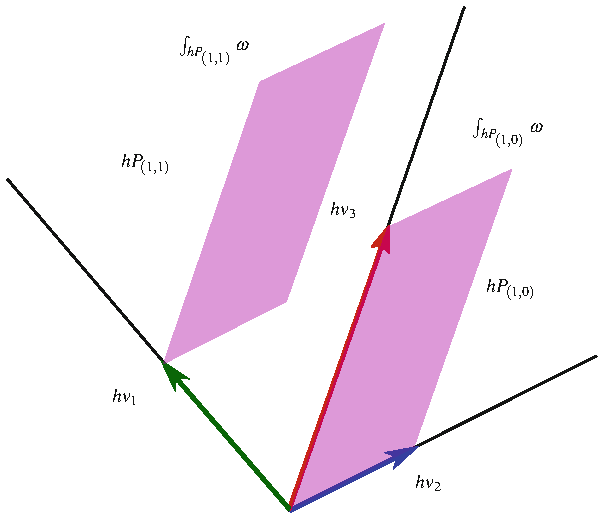
\includegraphics[width=0.803\linewidth]{images/vector/fig-4-4.pdf}
  \caption{这里显示了由 $hv_1,hv_2,hv_3$ 张成的平行六面体 $hP$ 的两个面 $hP_{(1,0)}$ 和 $hP_{(1,1)}$. 2-形式 $\omega$ 在这两个面上分别积分. 这两个积分之差 $\int_{hP_{(1,1)}}\omega-\int_{hP_{(1,0)}}\omega$ 给出 $\omega$ 的"总量"在 $v_1$ 方向变化的度量. 由于显然我们积分所用的 $hP$ 的面以及度量变化所用的方向 $v_1$ 都依赖于 $P$, 我们说我们度量的是 $\omega$ 的"总量"相对于 $P$ 在 $v_1$ 方向上的变化}
  \label{fig:4-4}
\end{figure}

\begin{figure}[htbp]
  \centering
  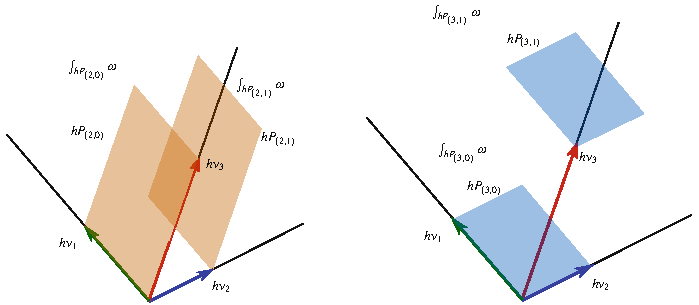
\includegraphics[width=0.960\linewidth]{images/vector/fig-4-5.pdf}
  \caption{在左侧, 我们求两个积分之差 $\int_{hP_{(2,1)}}\omega-\int_{hP_{(2,0)}}\omega$, 它给出 $\omega$ 的"总量"相对于 $P$ 在 $v_2$ 方向变化的度量. 类似地, 在右侧, 我们求两个积分之差 $\int_{hP_{(3,1)}}\omega-\int_{hP_{(3,0)}}\omega$, 它给出 $\omega$ 的"总量"相对于 $P$ 在 $v_3$ 方向变化的度量}
  \label{fig:4-5}
\end{figure}

以类似的方式, 积分之差 $\int_{hP_{(2,1)}}\omega-\int_{hP_{(2,0)}}\omega$ 给出 $\omega$ 的"总量"相对于平行六面体 $P$ 在 $v_2$ 方向变化的度量, 而积分之差 $\int_{hP_{(3,1)}}\omega-\int_{hP_{(3,0)}}\omega$ 给出 $\omega$ 的"总量"相对于平行六面体 $P$ 在 $v_3$ 方向变化的度量. 见图~\ref{fig:4-5}.

通过取 $\frac{1}{h^3}\left(\int_{hP_{(1,1)}}\omega-\int_{hP_{(1,0)}}\omega\right)$ 当 $h\to 0$ 时的极限, 我们实际上是在求 $\omega$ 的"总量"相对于 $P$ 在基点处沿 $v_1$ 方向的变化率. （回顾, 在上面的计算中, 我们曾不失一般性地假设向量 $v_1,\ldots,v_k$ 的基点是原点, 但一般来说基点可以是流形上的任意点.）$\frac{1}{h^3}\left(\int_{hP_{(2,1)}}\omega-\int_{hP_{(2,0)}}\omega\right)$ 和 $\frac{1}{h^3}\left(\int_{hP_{(3,1)}}\omega-\int_{hP_{(3,0)}}\omega\right)$ 当 $h\to 0$ 时的极限也分别求出 $\omega$ 的"总量"在基点处相对于由向量 $v_1,v_2,v_3$ 张成的平行六面体 $P$ 沿 $v_2$、$v_3$ 方向的变化率. 然后在此基础上, 我们把各种变化率相加/相减. 是加还是减按照 $P$ 各面的定向进行. 这将在第 11 章详细解释.

我们在特定点对 $d\omega(v_1,v_2,v_3)$ 实际得到的数, 是 $\omega$ 的"总量"在 $v_1$、$v_2$、$v_3$ 方向的各种变化率的某种奇怪的组合, 其中那些"总量"是用由向量 $v_1,v_2,v_3$ 张成的平行六面体的面来计算的. 因此数 $d\omega(v_1,v_2,v_3)$ 是 $\omega$ 的"总量"在基点处的一个总变化率, 它依赖于 $v_1,v_2,v_3$. 最终的这个数对你来说可能看起来有点奇怪, 但求它的所有组成部分都有非常清晰合理的几何意义. 当然, $d\omega$ 本身是一个 3-形式, 它使我们能够通过在给定点代入三个向量 $v_1,v_2,v_3$ 来计算该点的这个总变化率.

除了对"$\omega$ 的总量"这个说法获得一种感受之外, 使用这个定义给出了 $k$-形式外微分最具体的几何意义. 我们并没有试图在这里解释我们说"$\omega$ 的总量"是什么意思, 除了简单地说它是 $\omega$ 在 $P$ 的一个面上的积分. 形式的积分将在第 7 章至第 11 章解释. 特别是, 我们将在第 7.2 节从 Riemann 和的角度考察形式的积分, 这让我们对形式的积分在做什么有一个非常好的想法. 然而, 在三维情形中, 形式的积分有一些非常好的几何图景, 可以用来获得对正在发生之事的直观理解. 这些图景依赖于 1-形式、2-形式和 3-形式如何被可视化（这在第 5 章讨论）, 以及 Stokes 定理（在第 11 章讨论）. 我们将在第 11.6 节末尾回到对 1-形式、2-形式和 3-形式外微分几何的探索. 虽然对 $k>3$ 不再有帮助我们可视化微分形式的漂亮图景, 但 $n$ 维流形上 $k$-形式外微分的几何意义是类似的；只是需要考虑更多方向和 $P$ 的面, 而且 $P$ 的所有面都是 $k$ 维的.

$n$-形式 $\omega$ 的外微分的这个特定定义也给出了广义 Stokes 定理为什么成立的最清晰的直观想法. 使用这个定义, 
\begin{align*}
d\omega\bigl(v_1,\ldots,v_{k+1}\bigr)=\lim_{h\to 0}\frac{1}{h^{k+1}}\int_{\partial(hP)}\omega \\
\Longleftrightarrow
\end{align*}
当 $h$ 非常小时, 
\begin{align*}
d\omega\bigl(v_1,\ldots,v_{k+1}\bigr)\approx\frac{1}{h^{k+1}}\int_{\partial(hP)}\omega \\
\Longleftrightarrow
\end{align*}
两边同乘以 $h^{k+1}$, 
\begin{align*}
\underbrace{h^{k+1}}_{\text{一个数}}d\omega\bigl(v_1,\ldots,v_{k+1}\bigr)\approx\int_{\partial(hP)}\omega \\
\Longleftrightarrow
\end{align*}
$hP$ 的体积近似为 $h^{k+1}$, 
\begin{align*}
d\omega\bigl(v_1,\ldots,v_{k+1}\bigr)\underbrace{\int_{hP}dx_1\wedge\cdots\wedge dx_{k+1}}_{\text{体积形式}}\approx\int_{\partial(hP)}\omega \\
\Longleftrightarrow
\end{align*}
把这个数放到积分号里面, 
\begin{align*}
\int_{hP}d\omega\bigl(v_1,\ldots,v_{k+1}\bigr)\,dx_1\wedge\cdots\wedge dx_{k+1}\approx\int_{\partial(hP)}\omega \\
\Longleftrightarrow
\end{align*}
把左端写成抽象记号, 
\begin{align*}
\int_{hP}d\omega\approx\int_{\partial(hP)}\omega \\
\Longleftrightarrow
\end{align*}
令 $h\to 0$, 
\[
\int_{hP}d\omega=\int_{\partial(hP)}\omega.
\]
最后的蕴含给出区域 $hP$ 上的广义 Stokes 定理. 这当然不是一个严格的证明, 那在第 11 章完成, 但它的确提供了广义 Stokes 定理是什么的一个非常好的大图景, 以及它为什么成立的合理几何论证.

\begin{question}\label{q:4-9}
类似于上面的讨论, 解释 $n$ 维流形上 3-形式 $\omega$ 的 $d\omega(v_1,v_2,v_3,v_4)$ 的几何意义.
\end{question}

\begin{question}\label{q:4-10}
类似于上面的讨论, 解释 $n$ 维流形上 $k$-形式 $\omega$ 的 $d\omega(v_1,\ldots,v_k)$ 的几何意义.
\end{question}

\section{外微分例题}

现在我们转而利用前面几节得到的各种公式. 习惯外微分运算最简单的方式可能就是看一系列例子并亲手算一遍. 做这些计算时, 我们将相当详细, 只是为了让你习惯并熟悉一切. 一旦你熟悉了这类计算, 你就可以毫无问题地跳过许多步骤.

设我们有两个函数 $f,g:\mathbb{R}^2\to\mathbb{R}$. 我们想求 $df\wedge dg$. 首先我们注意到有
\[
df=\frac{\partial f}{\partial x}dx+\frac{\partial f}{\partial y}dy
\qquad\text{和}\qquad
dg=\frac{\partial g}{\partial x}dx+\frac{\partial g}{\partial y}dy.
\]
然后我们取这两个 1-形式的楔积, 并使用第 3.3.1 节给出的楔积的代数性质: 
\begin{align*}
df\wedge dg&=\left(\frac{\partial f}{\partial x}dx+\frac{\partial f}{\partial y}dy\right)
\wedge\left(\frac{\partial g}{\partial x}dx+\frac{\partial g}{\partial y}dy\right)\\
&=\frac{\partial f}{\partial x}dx\wedge\left(\frac{\partial g}{\partial x}dx+\frac{\partial g}{\partial y}dy\right)
+\frac{\partial f}{\partial y}dy\wedge\left(\frac{\partial g}{\partial x}dx+\frac{\partial g}{\partial y}dy\right)\\
&=\frac{\partial f}{\partial x}\frac{\partial g}{\partial x}\underbrace{dx\wedge dx}_{=0}
+\frac{\partial f}{\partial x}\frac{\partial g}{\partial y}dx\wedge dy
+\frac{\partial f}{\partial y}\frac{\partial g}{\partial x}dy\wedge dx
+\frac{\partial f}{\partial y}\frac{\partial g}{\partial y}\underbrace{dy\wedge dy}_{=0}\\
&=\frac{\partial f}{\partial x}\frac{\partial g}{\partial y}dx\wedge dy
+\frac{\partial f}{\partial y}\frac{\partial g}{\partial x}dy\wedge dx\\
&=\frac{\partial f}{\partial x}\frac{\partial g}{\partial y}dx\wedge dy
-\frac{\partial f}{\partial y}\frac{\partial g}{\partial x}dx\wedge dy\\
&=\left(\frac{\partial f}{\partial x}\frac{\partial g}{\partial y}-\frac{\partial f}{\partial y}\frac{\partial g}{\partial x}\right)dx\wedge dy\\
&=\begin{vmatrix}\frac{\partial f}{\partial x}&\frac{\partial f}{\partial y}\\[4pt]\frac{\partial g}{\partial x}&\frac{\partial g}{\partial y}\end{vmatrix}dx\wedge dy.
\end{align*}
所以, $df$ 和 $dg$ 的楔积在二维体积形式（面积形式）$dx\wedge dy$ 前面带有来自向量微积分的 Jacobian 矩阵. 换句话说, 我们找到了恒等式
\[
df\wedge dg=\underbrace{\begin{vmatrix}\frac{\partial f}{\partial x}&\frac{\partial f}{\partial y}\\[4pt]\frac{\partial g}{\partial x}&\frac{\partial g}{\partial y}\end{vmatrix}}_{\text{Jacobian 矩阵}}\underbrace{dx\wedge dy}_{\text{面积形式}}.
\]

证明对 $f,g,h:\mathbb{R}^3\to\mathbb{R}$ 有
\[
df\wedge dg\wedge dh
=\underbrace{\begin{vmatrix}\frac{\partial f}{\partial x}&\frac{\partial f}{\partial y}&\frac{\partial f}{\partial z}\\[4pt]\frac{\partial g}{\partial x}&\frac{\partial g}{\partial y}&\frac{\partial g}{\partial z}\\[4pt]\frac{\partial h}{\partial x}&\frac{\partial h}{\partial y}&\frac{\partial h}{\partial z}\end{vmatrix}}_{\text{Jacobian 矩阵}}
\underbrace{dx\wedge dy\wedge dz}_{\text{体积形式}}
\]
也许有点繁琐, 但并不困难. 显然的推广也成立. 然而, 用楔积的性质证明一般公式相当繁琐. 相反, 我们将把这个公式的证明推迟到以后, 等到引入了更多的数学工具、我们能够给出更漂亮的证明时再证明.

\begin{question}\label{q:4-11}
给定函数 $f,g,h:\mathbb{R}^3\to\mathbb{R}$, 求出上面 $df\wedge dg\wedge dh$ 的恒等式.
\end{question}

现在我们来看一个例子, 其中有两个明确给出的函数. 例如, 假设我们有由 $f:\mathbb{R}^2\to\mathbb{R}$, $f(x,y)=x+y$ 和 $g:\mathbb{R}^2\to\mathbb{R}$, $g(x,y)=x-y$ 给出的坐标变换. 为了求 $df\wedge dg$, 我们可以采取两种方法之一. 例如, 我们可以先求 $df$ 和 $dg$, 然后用微分形式的代数性质来化简, 或者我们可以直接跳到上面找到的恒等式. 我们将演示两种方法. 采用第一种方法, 首先求出 $df$ 和 $dg$, 我们有
\[
df=\frac{\partial f}{\partial x}dx+\frac{\partial f}{\partial y}dy
=\frac{\partial(x+y)}{\partial x}dx+\frac{\partial(x+y)}{\partial y}dy=dx+dy
\]
和
\[
dg=\frac{\partial g}{\partial x}dx+\frac{\partial g}{\partial y}dy
=\frac{\partial(x-y)}{\partial x}dx+\frac{\partial(x-y)}{\partial y}dy=dx-dy.
\]
然后使用微分形式的代数性质化简, 我们发现
\begin{align*}
df\wedge dg&=(dx+dy)\wedge(dx-dy)\\
&=dx\wedge(dx-dy)+dy\wedge(dx-dy)\\
&=\underbrace{dx\wedge dx}_{=0}-dx\wedge dy+dy\wedge dx-\underbrace{dy\wedge dy}_{=0}\\
&=-dx\wedge dy-dx\wedge dy\\
&=-2\,dx\wedge dy.
\end{align*}
在第二种方法中, 我们只使用前面找到的恒等式得到
\begin{align*}
df\wedge dg&=\begin{vmatrix}\frac{\partial f}{\partial x}&\frac{\partial f}{\partial y}\\[4pt]\frac{\partial g}{\partial x}&\frac{\partial g}{\partial y}\end{vmatrix}dx\wedge dy\\
&=\begin{vmatrix}\frac{\partial(x+y)}{\partial x}&\frac{\partial(x+y)}{\partial y}\\[4pt]\frac{\partial(x-y)}{\partial x}&\frac{\partial(x-y)}{\partial y}\end{vmatrix}dx\wedge dy\\
&=\begin{vmatrix}1&1\\1&-1\end{vmatrix}dx\wedge dy\\
&=-2\,dx\wedge dy.
\end{align*}
我们的两个答案一致, 这一点也不令人惊讶.

让我们用另一个涉及更复杂函数的例子深入一些. 考虑由 $f:\mathbb{R}^2\to\mathbb{R}$, $f(x,y)=x^2y+x$ 和 $g:\mathbb{R}^2\to\mathbb{R}$, $g(x,y)=x^2y^3+2xy$ 给出的函数. 我们使用我们的恒等式: 
\[
\begin{aligned}
df\wedge dg&=\begin{vmatrix}(2xy+1)&x^2\$2xy^3+2y)&(3x^2y^2+2x)\end{vmatrix}dx\wedge dy\\
&=\Bigl((2xy+1)(3x^2y^2+2x)-x^2(2xy^3+2y)\Bigr)dx\wedge dy.
\end{aligned}
\]
这是我们整个流形 $\mathbb{R}^2$ 上的 $df\wedge dg$. 假设我们想知道 $df\wedge dg$ 在流形的某个特定点处是什么？我们不得不代入该点的值. 例如, 假设我们想求流形 $\mathbb{R}^2$ 上点 $p=(1,1)$ 处的 $df\wedge dg$. 我们代入得到
\begin{align*}
\bigl(df\wedge dg\bigr)_{p=(1,1)}
&=\Bigl[\bigl(2\cdot 1\cdot 1+1\bigr)\bigl(3\cdot 1^2\cdot 1^2+2\cdot 1\bigr)-1^2\bigl(2\cdot 1\cdot 1^3+2\cdot 1\bigr)\Bigr]dx\wedge dy\\
&=\bigl[(3)(5)-(4)\bigr]dx\wedge dy\\
&=11\,dx\wedge dy.
\end{align*}
类似地, 如果我们想求流形 $\mathbb{R}^2$ 上点 $p=(-1,2)$ 处的 $df\wedge dg$, 我们代入得到
\begin{align*}
\bigl(df\wedge dg\bigr)_{p=(-1,2)}
&=\Bigl[\bigl(2\cdot(-1)\cdot 2+1\bigr)\bigl(3\cdot(-1)^2\cdot 2^2+2\cdot(-1)\bigr)\\
&\qquad\qquad-(-1)^2\bigl(2\cdot(-1)\cdot 2^3+2\cdot(-1)\bigr)\Bigr]dx\wedge dy\\
&=\bigl[(-3)(10)-(-18)\bigr]dx\wedge dy\\
&=-12\,dx\wedge dy.
\end{align*}
现在假设我们有两个向量 $v_p=\binom{-2}{3}_{\!(1,1)}$ 和 $w_p=\binom{-4}{-2}_{\!(1,1)}$, 想求 $(df\wedge dg)(v_p,w_p)$. 在第一个等式之后省略基点 $(1,1)$ 的书写, 我们得到
\begin{align*}
\bigl(df\wedge dg\bigr)_{(1,1)}\left(\binom{-2}{3}_{\!(1,1)},\binom{-4}{-2}_{\!(1,1)}\right)
&=11\,dx\wedge dy\left(\binom{-2}{3},\binom{-4}{-2}\right)\\
&=11\cdot\begin{vmatrix}dx\left(\binom{-2}{3}\right)&dx\left(\binom{-4}{-2}\right)\\[4pt]dy\left(\binom{-2}{3}\right)&dy\left(\binom{-4}{-2}\right)\end{vmatrix}\\
&=11\cdot\begin{vmatrix}-2&-4\\3&-2\end{vmatrix}\\
&=11(4+12)\\
&=176.
\end{align*}
如果我们有向量 $v_p=\binom{3}{1}_{\!(-1,2)}$ 和 $w_p=\binom{1}{2}_{\!(-1,2)}$, 想求 $(df\wedge dg)(v_p,w_p)$, 我们会有
\[
\bigl(df\wedge dg\bigr)_{(-1,2)}\left(\binom{3}{1}_{\!(-1,2)},\binom{1}{2}_{\!(-1,2)}\right)
=-12\begin{vmatrix}3&1\\1&2\end{vmatrix}=-60.
\]

现在我们再做一你可能觉得有点眼熟的例子. 若 $x=r\cos(\theta)$ 和 $y=r\sin(\theta)$, 用 $d\theta\wedge dr$ 写出 $dx\wedge dy$. 这样做给出
\begin{align*}
dx\wedge dy&=\begin{vmatrix}\frac{dx}{d\theta}&\frac{dx}{dr}\\[4pt]\frac{dy}{d\theta}&\frac{dy}{dr}\end{vmatrix}d\theta\wedge dr\\
&=\begin{vmatrix}\frac{d(r\cos(\theta))}{d\theta}&\frac{d(r\cos(\theta))}{dr}\\[4pt]\frac{d(r\sin(\theta))}{d\theta}&\frac{d(r\sin(\theta))}{dr}\end{vmatrix}d\theta\wedge dr\\
&=\begin{vmatrix}-r\sin(\theta)&\cos(\theta)\\r\cos(\theta)&\sin(\theta)\end{vmatrix}d\theta\wedge dr\\
&=\Bigl(-r\sin^2(\theta)-r\cos^2(\theta)\Bigr)d\theta\wedge dr\\
&=-r\,d\theta\wedge dr.
\end{align*}
如果你觉得这看起来有点像极坐标换元公式, 那你完全正确. 我们很快会更详细地讨论这一点.

\begin{question}\label{q:4-12}
设 $f,g,h:\mathbb{R}^3\to\mathbb{R}$ 由 $f(x,y,z)=x^2y$、$g(x,y,z)=y^2z^2$、$h(x,y,z)=xyz$ 定义.
\begin{enumerate}
  \item[(a)] 求 $df\wedge dg\wedge dh$.
  \item[(b)] 求点 $p=(-1,1,-1)$ 处的 $df\wedge dg\wedge dh$.
  \item[(c)] 求 $df\wedge dg\wedge dh_{(-1,1,-1)}(u_p,v_p,w_p)$, 其中
  \[
  u_p=\begin{bmatrix}1\\2\\3\end{bmatrix}_{\!(-1,1,-1)},\qquad
  v_p=\begin{bmatrix}-1\\0\\1\end{bmatrix}_{\!(-1,1,-1)},\qquad
  w_p=\begin{bmatrix}-2\\-1\\0\end{bmatrix}_{\!(-1,1,-1)}.
  \]
\end{enumerate}
\end{question}

在最后几个例子和问题中, 我们处理了非常特定类型的问题. 注意我们拥有的函数数目（两个或三个）与函数所定义流形的维数相同. 例如, 在流形 $\mathbb{R}^2$ 上有两个函数 $f$ 和 $g$. 在流形 $\mathbb{R}^3$ 上有三个函数 $f,g,h$. 于是, 在第一种情形中 $df\wedge dg$ 给我们一个函数乘以二维体积形式 $dx\wedge dy$, 而在第二种情形中 $df\wedge dg\wedge dh$ 给我们一个函数乘以三维体积形式. 现在我们来看一些更一般的例子.

\begin{question}\label{q:4-13}
设 $f,g:\mathbb{R}^3\to\mathbb{R}$ 由 $f(x,y,z)=x^2y^3z^2$ 和 $g(x,y,z)=xyz^2$ 给出.
\begin{enumerate}
  \item[(a)] 求 $df$ 和 $dg$.
  \item[(b)] 求 $df\wedge dg$. （注意, 你不能再使用 Jacobian 矩阵, 你必须使用上面求出的 $df$ 和 $dg$, 以及楔积的代数性质.）
  \item[(c)] 求点 $(3,2,1)$ 处的 $df\wedge dg$.
  \item[(d)] 设 $v_p=\begin{bmatrix}-1\\0\\1\end{bmatrix}$ 和 $w_p=\begin{bmatrix}-2\\1\\-1\end{bmatrix}$. 求 $df\wedge dg(v_p,w_p)$.
\end{enumerate}
\end{question}

现在我们转向一些求 1-形式外微分的例子. 设 $\varphi=x^2yz\,dx$ 是 $\mathbb{R}^3$ 上的 1-形式. 我们将使用上一节的公式求 $d\varphi$: 
\begin{align*}
d\varphi&=d\bigl(x^2yz\bigr)\wedge dx\\
&=\left(\frac{\partial(x^2yz)}{\partial x}dx+\frac{\partial(x^2yz)}{\partial y}dy+\frac{\partial(x^2yz)}{\partial z}dz\right)\wedge dx\\
&=\bigl(2xyz\,dx+x^2z\,dy+x^2y\,dz\bigr)\wedge dx\\
&=2xyz\underbrace{dx\wedge dx}_{=0}+x^2z\,dy\wedge dx+x^2y\,dz\wedge dx\\
&=-x^2z\,dx\wedge dy-x^2y\,dx\wedge dz.
\end{align*}

对我们的下一个例子, 设 $\varphi=\sin(x)dx+e^x\cos(y)dy+3xy\,dz$. 我们将分三步求 $d\varphi$, 对 $\varphi$ 的每一项一步: 
\[
d\varphi=\underbrace{d\bigl(\sin(x)\bigr)\wedge dx}_{(1)}
+\underbrace{d\bigl(e^x\cos(y)\bigr)\wedge dy}_{(2)}
+\underbrace{d\bigl(3xy\bigr)\wedge dz}_{(3)}.
\]
第一项给出
\begin{align*}
d\bigl(\sin(x)\bigr)\wedge dx
&=\left(\frac{\partial\sin(x)}{\partial x}dx+\frac{\partial\sin(x)}{\partial y}dy+\frac{\partial\sin(x)}{\partial z}dz\right)\wedge dx\\
&=\bigl(\cos(x)dx+0\,dy+0\,dz\bigr)\wedge dx\\
&=\cos(x)\underbrace{dx\wedge dx}_{=0}\\
&=0.
\end{align*}
第二项给出
\begin{align*}
d\bigl(e^x\cos(y)\bigr)\wedge dy
&=\left(\frac{\partial(e^x\cos(y))}{\partial x}dx+\frac{\partial(e^x\cos(y))}{\partial y}dy+\frac{\partial(e^x\cos(y))}{\partial z}dz\right)\wedge dy\\
&=e^x\cos(y)\,dx\wedge dy-e^x\sin(y)\underbrace{dy\wedge dy}_{=0}+0\,dz\wedge dy\\
&=e^x\cos(y)\,dx\wedge dy.
\end{align*}
第三项给出
\begin{align*}
d\bigl(3xy\bigr)\wedge dz
&=\left(\frac{\partial 3xy}{\partial x}dx+\frac{\partial 3xy}{\partial y}dy+\frac{\partial 3xy}{\partial z}dz\right)\wedge dz\\
&=3y\,dx\wedge dz+3x\,dy\wedge dz+0\,dz\wedge dz\\
&=3x\,dy\wedge dz-3y\,dz\wedge dx.
\end{align*}
把一切组合起来, 我们有
\[
d\varphi=e^x\cos(y)\,dx\wedge dy+3x\,dy\wedge dz-3y\,dz\wedge dx.
\]

\begin{question}\label{q:4-14}
若 $\varphi=f_1\,dx_1+f_2\,dx_2+f_3\,dx_3$, 求 $d\varphi$ 的公式.
\end{question}

你对上一个问题的答案应该是
\[
d\varphi=\left(\frac{\partial f_2}{\partial x_1}-\frac{\partial f_1}{\partial x_2}\right)dx_1\wedge dx_2
+\left(\frac{\partial f_3}{\partial x_1}-\frac{\partial f_1}{\partial x_3}\right)dx_1\wedge dx_3
+\left(\frac{\partial f_3}{\partial x_2}-\frac{\partial f_2}{\partial x_3}\right)dx_2\wedge dx_3.
\]

接下来我们证明, 如果 $f,g$ 是 $\mathbb{R}^n$ 上的函数, 则 $d(f\cdot g)=df\cdot g+f\cdot dg$.
\begin{align*}
d(f\cdot g)&=\sum_i\frac{\partial f\cdot g}{\partial x_i}dx_i\\
&\overset{\text{积法则}}{=}\sum_i\left(\frac{\partial f}{\partial x_i}\cdot g+f\cdot\frac{\partial g}{\partial x_i}\right)dx_i\\
&=\sum_i g\cdot\frac{\partial f}{\partial x_i}dx_i+\sum_i f\cdot\frac{\partial g}{\partial x_i}dx_i\\
&=g\cdot df+f\cdot dg.
\end{align*}
这实际上只不过是用稍微不同的记号写出的乘积法则.

\begin{question}\label{q:4-15}
证明外微分 $d$ 具有线性性质, 即若 $\varphi=\sum f_i\,dx_i$ 和 $\psi=\sum g_i\,dx_i$, 则对 $a,b\in\mathbb{R}$, 
\[
d(a\varphi+b\psi)=a\,d\varphi+b\,d\psi.
\]
\end{question}

\begin{question}\label{q:4-16}
如果 $f$ 是一个函数, $\varphi$ 是一个 1-形式, 证明
\[
d(f\varphi)=df\wedge\varphi+f\,d\varphi.
\]
\end{question}

\begin{question}\label{q:4-17}
如果 $\varphi,\psi$ 是 1-形式, 证明
\[
d(\varphi\wedge\psi)=d\varphi\wedge\psi+\varphi\wedge d\psi.
\]
\end{question}

注意, 在运算顺序上, 乘法和楔积优先于加法和减法.

接下来我们证明, 如果 $f$ 是 $\mathbb{R}^n$ 上的函数, 则 $ddf=0$. 这意味着无论 $f$ 是什么, 取两次外微分都给出 0. 首先, 我们知道 $df=\sum_i\frac{\partial f}{\partial x_i}dx_i$, 所以
\begin{align*}
ddf&=d\left(\sum_i\frac{\partial f}{\partial x_i}dx_i\right)\\
&=\sum_i d\left(\frac{\partial f}{\partial x_i}\right)\wedge dx_i\\
&=\sum_i\sum_j\frac{\partial}{\partial x_j}\left(\frac{\partial f}{\partial x_i}\right)dx_j\wedge dx_i\\
&=\sum_{i,j}\frac{\partial^2 f}{\partial x_j\partial x_i}dx_j\wedge dx_i\\
&=\sum_{i<j}\left(\frac{\partial^2 f}{\partial x_j\partial x_i}-\frac{\partial^2 f}{\partial x_i\partial x_j}\right)dx_i\wedge dx_j\\
&=\sum_{i<j}\underbrace{\left(\frac{\partial^2 f}{\partial x_j\partial x_i}-\frac{\partial^2 f}{\partial x_i\partial x_j}\right)}_{=0\ \text{（由混合偏导数的相等）}}dx_i\wedge dx_j\\
&=0.
\end{align*}

\begin{question}\label{q:4-18}
对函数 $f,g$, 证明 $d(f\,dg)=df\wedge dg$.
\end{question}

\begin{question}\label{q:4-19}
化简
\begin{enumerate}
  \item[(a)] $d\bigl(f\,dg+f\,df\bigr)$, 
  \item[(b)] $d\bigl((f-g)(df+dg)\bigr)$, 
  \item[(c)] $d\bigl((f\,dg)\wedge(g\,df)\bigr)$, 
  \item[(d)] $d(gf\,df)+d(f\,dg)$.
\end{enumerate}
\end{question}

正如我们前面提到的, 我们到目前为止的简化之一是坚持使用标准笛卡尔坐标系. 考虑到大多数学生对笛卡尔坐标系的熟悉程度, 在一个大多数学生完全适应的场所引入像微分形式、楔积和外微分这样复杂的思想是有意义的. 我们不希望因为你陷入其他坐标系细节的泥潭而看不到大思想. 然而, 其他坐标系很快就将对我们发挥越来越重要的作用.

\section{小结、参考文献与问题}

\subsection{小结}

在本章中, 我们探索了外微分的四种不同方法. 在第一种方法中, 给出了外微分的局部公式, 即使用坐标的公式, 
\[
d\Bigl(\sum \alpha_{i_1\cdots i_n}\,dx_{i_1}\wedge\cdots\wedge dx_{i_n}\Bigr)
=\sum\sum_{j=1}^{n}\frac{\partial\alpha_{i_1\cdots i_n}}{\partial x_{i_j}}dx_{i_j}\wedge dx_{i_1}\wedge\cdots\wedge dx_{i_n}.
\]
使用这个局部公式, 可以证明下列代数性质成立: 
\begin{enumerate}
  \item $d(\alpha+\beta)=d\alpha+d\beta$, 
  \item $d(\alpha\wedge\omega)=d\alpha\wedge\omega+(-1)^n\alpha\wedge d\omega$, 
  \item 对每个 $n$-形式 $\alpha$, $d(d\alpha)=0$.
\end{enumerate}
定义外微分的第二种方法基本上与此相反. 三条性质被作为定义性公理给出, 然后从这些性质推导出坐标中的唯一公式.

外微分的第三种方法是试图找到一个整体公式. 整体公式与局部公式的不同之处在于它不依赖坐标. 也就是说, 坐标不出现在公式中. 首先用常向量场找到 $k$-形式外微分的整体公式, 
\[
d\omega(v_0,\ldots,v_k)=\sum_i(-1)^i\,v_i\bigl[\omega(v_0,\ldots,\widehat{v_i},\ldots,v_k)\bigr].
\]
利用两个向量场的李括号的定义
\[
[v,w]F=v\bigl[w[F]\bigr]-w\bigl[v[F]\bigr],
\]
对非常值向量场找到 1-形式外微分的整体公式, 
\[
d\alpha(v,w)=v[\alpha(w)]-w[\alpha(v)]-\alpha([v,w]).
\]
然后给出非常值向量场情形下 $k$-形式外微分的一般整体公式, 
\[
\begin{aligned}
d\alpha(v_0,\ldots,v_k)&=\sum_i(-1)^i\,v_i\bigl[\alpha(v_0,\ldots,\widehat{v_i},\ldots,v_k)\bigr]\\
&\qquad+\sum_{i<j}(-1)^{i+j}\,\alpha\bigl([v_i,v_j],v_0,\ldots,\widehat{v_i},\ldots,\widehat{v_j},\ldots,v_k\bigr).
\end{aligned}
\]
这个公式实际上直到第 A.7 节才被证明.

外微分的第四种方法是一种非常几何的方法, 其中 $k$-形式在某点的外微分被定义为
\[
d\omega\bigl(v_1,\ldots,v_{k+1}\bigr)=\lim_{h\to 0}\frac{1}{h^{k+1}}\int_{\partial(hP)}\omega.
\]
这个几何定义将在第 11.6 节重新讨论, 以便在三维情形下获得对几何的更深入理解. 外微分的这个几何定义也为 Stokes 定理为什么成立提供了最几何化的论证（虽然不是证明）.

\subsection{参考文献与进一步阅读}

如概述所解释的, 在大多数书中, 外微分通常以四种方式之一来处理. 与楔积一样, 这是可以理解的, 因为外微分只是需要覆盖的众多不同主题之一. 然而, 我们已尽可能地把一切整合在一起, 探索外微分的所有这些方法, 使读者对他们将来可能遇到的任何外微分方法都完全感到舒服. 例如, O'Neill~\cite{ref36} 使用局部坐标方法, 而 Tu~\cite{ref46} 在书的早期从局部坐标角度涵盖外微分, 然后在书的中部从整体角度加以涵盖. Martin~\cite{ref33}、Darling~\cite{ref12} 和 Flanders~\cite{ref19} 都使用基于公理的方法. 外导数的几何观点相当罕见, 据我们所知, 唯一真正把它用作引入外微分方法的地方是 Hubbard 和 Hubbard~\cite{ref27}, 尽管外导数的这种几何意义在 Darling~\cite{ref12} 和 Arnold~\cite{ref03} 中也被简短地提及. 我们的论述在很大程度上遵循 Hubbard 和 Hubbard, 但没有他们那么完整或详细.

\subsection{问题}

\begin{question}\label{q:4-20}
设 $f_1(x,y,z)=x^3y^2z-2xyz^3$、$f_2(x,y,z)=x^2-3y^2+6z^4$、$f_3(x,y,z)=xy^2+yz^2+zx^2$、$f_4(x,y,z)=3x-2y+5z-4$. 求 $df_1$、$df_2$、$df_3$ 和 $df_4$.
\end{question}

\begin{question}\label{q:4-21}
设 $g_1(x,y,z)=\frac{x^2+y^2}{z}$、$g_2(x,y,z)=\sin(x^2+y^2)+\tan(2z)$、$g_3(x,y,z)=xz+ye^y+3x-2$、$g(x,y,z)=\cos(xy^2z)+\frac{x^2}{yz}$. 求 $dg_1$、$dg_2$ 和 $dg_3$.
\end{question}

\begin{question}\label{q:4-22}
对问题~\ref{q:4-20} 和问题~\ref{q:4-21} 中的函数, 求 $d(2f_1+3g_1)$、$d(5f_2+3g_2)$、$d(-2f_3-5g_3)$ 和 $d(7f_4-3g_3)$.
\end{question}

\begin{question}\label{q:4-23}
对问题~\ref{q:4-20} 中的函数, 求 $d(f_1\cdot f_2)$、$d(f_1\cdot f_3)$、$d(f_1\cdot f_4)$、$d(f_2\cdot f_3)$、$d(f_2\cdot f_4)$ 和 $d(f_3\cdot f_4)$.
\end{question}

\begin{question}\label{q:4-24}
设 $\alpha_1=3x^3dx+\frac{x+y}{z}dy$、$\alpha_2=-x\,dx+(x-3y)dy$、$\alpha_3=\frac{x^3}{y}dx+xyz\,dx+(x^2+y^2+z^2)dz$、$\alpha_4=y^2z\,dx-xz\,dy+(3x+2)dz$. 求 $d\alpha_1$、$d\alpha_2$、$d\alpha_3$ 和 $d\alpha_4$.
\end{question}

\begin{question}\label{q:4-25}
设 $\beta_1=\sin(x)dx+\sin(y)dy-\cos(z)dz$、$\beta_2=\sin(xyz)dx-\cos(x^2)dy+e^y\,dz$、$\beta_3=\sin^2(xz)dx+\cos^3(yz)dy-e^{xy}dz$、$\beta_4=(x^2+y^2+z^2)dx-xz\,dy-xz\,e^y\,dz$. 求 $d\beta_1$、$d\beta_2$、$d\beta_3$ 和 $d\beta_4$.
\end{question}

\begin{question}\label{q:4-26}
对问题~\ref{q:4-24} 和问题~\ref{q:4-25} 中的 1-形式, 求 $d(2\alpha_1+3\beta_1)$、$d(5\alpha_2+3\beta_2)$、$d(-2\alpha_3-5\beta_3)$ 和 $d(7\alpha_4-3\beta_3)$.
\end{question}

\begin{question}\label{q:4-27}
对问题~\ref{q:4-20} 中的函数和问题~\ref{q:4-24} 中的 1-形式, 求 $d(f_1\alpha_1)$、$d(f_2\alpha_2)$、$d(f_3\alpha_3)$ 和 $d(f_4\alpha_4)$.
\end{question}

\begin{question}\label{q:4-28}
对问题~\ref{q:4-24} 和问题~\ref{q:4-25} 中的 1-形式, 求 $d(\alpha_1\wedge\beta_1)$、$d(\alpha_2\wedge\beta_2)$、$d(\alpha_3\wedge\beta_3)$ 和 $d(\alpha_4\wedge\beta_4)$.
\end{question}

\begin{question}\label{q:4-29}
对问题~\ref{q:4-20} 中的函数, 求 $d^2f_1$、$d^2f_2$、$d^2f_3$ 和 $d^2f_4$.
\end{question}

\begin{question}\label{q:4-30}
对问题~\ref{q:4-24} 中的 1-形式, 求 $d^2\alpha_1$、$d^2\alpha_2$、$d^2\alpha_3$ 和 $d^2\alpha_4$.
\end{question}

\begin{question}\label{q:4-31}
设 $\gamma_1=(x^2+y^4)dx\wedge dy+s^3y^2z^5\,dy\wedge dz-(3x+2y-4z+7)dz\wedge dx$ 和 $\gamma_2=xy\sin(z)dx\wedge dy-\cos(xyz)dy\wedge dz+\sin(xz)\cos(yz)dy\wedge dx$. 求 $d\gamma_1$、$d\gamma_2$ 和 $d(3\gamma_1-5\gamma_2)$. 然后求 $d^2\gamma_1$ 和 $d^2\gamma_2$.
\end{question}

\begin{question}\label{q:4-32}
如果 $f:\mathbb{R}^2\to\mathbb{R}$ 和 $g:\mathbb{R}\to\mathbb{R}$, 证明 $v_p\bigl[g(f)\bigr]=g'(f)\,v_p\bigl[f\bigr]$. 利用这一点推出 $d\bigl(g(f)\bigr)=g'(f)\,df$.
\end{question}

\begin{question}\label{q:4-33}
如果 $f$、$g$ 和 $h$ 是 $\mathbb{R}^2$ 上的实值函数, $\alpha$ 是 $\mathbb{R}^2$ 上的 1-形式, 证明 $d(fgh)=gh\,df+fh\,dg+fg\,dh$, 并且
\[
(df\wedge dg)(v,w)=v[f]w[g]-v[g]w[f].
\]
\end{question}

\begin{question}\label{q:4-34}
给定 $\mathbb{R}^6$ 上的 2-形式 $\alpha=x_1x_4x_6\,dx_1\wedge dx_5$、$\beta=x_2^3\sin(x_4)dx_3\wedge dx_5$ 和 $\gamma=(x_1^2+x_3^2+x_5^2)dx_2\wedge dx_6$, 求 $d\alpha$、$d\beta$、$d\gamma$、$d^2\alpha$、$d^2\beta$ 和 $d^2\gamma$. 现在假设 $\alpha$、$\beta$ 和 $\gamma$ 是 $\mathbb{R}^8$ 上的 2-形式, 求同样的外微分. 它们相同还是不同？解释为什么相同或为什么不同.
\end{question}

使用第 4.5 节给出的 0-形式在单个点的积分定义来回答下列问题.

\begin{question}\label{q:4-35}
设 $P=\{(3,2,1)\}\subset\mathbb{R}^3$, 设 $f=x^3y^2-z^3$ 是 $\mathbb{R}^3$ 上的 0-形式. 求 $\int_P f$.
\end{question}

\begin{question}\label{q:4-36}
设 $P=-\{(-1,2,-1)\}\subset\mathbb{R}^3$, $f=x(y-z+2)$. 求 $\int_P f$.
\end{question}

\begin{question}\label{q:4-37}
设 $P=\{(5,-5,3)\}\subset\mathbb{R}^3$, $f=x^3(xy^2+yz^2+3)$. 求 $\int_P f$.
\end{question}

\begin{question}\label{q:4-38}
设 $P=-\{(-4,2,7)\}\subset\mathbb{R}^3$, $f=2^xy^z$. 求 $\int_P f$.
\end{question}

% 第 5 章 可视化一、二、三形式
\chapter{可视化一、二、三形式}

在本章中，我们将引入并详细讨论物理学家有时用来可视化"良好"微分形式的一种方式. 本质上，我们将考虑在向量空间上可视化一形式、二形式与三形式的方法. 也就是说，我们将找到 $\alpha_p\in T_p^*\mathbb{R}^2$ 与 $\alpha_p\in T_p^*\mathbb{R}^3$ 的"漫画图". 我们对 $\alpha_p$ 的图将叠加在向量空间 $T_p\mathbb{R}^3$ 上. 这一视角在 Misner、Thorne 和 Wheeler 的巨著 \textit{Gravitation} 中得到了充分的发展. 事实上，他们也做出了一些努力来发展（时空的）四维图形，不过我们在这里将主要限于二维与三维的情形. 第 1 节集中讨论二维的情形，第 2 至第 4 节讨论三维的情形. 然后在第 5 节我们把我们的漫画图推广到一般的二维与三维流形. 再说一遍，这种漫画图实际上只适用于"良好"的微分形式，即物理学家更可能遇到的那种微分形式，但对于不太复杂的微分形式与流形，它仍然是有用的. 最后，在第 6 节我们引入 Hodge 星算子. 我们在三维中对形式的可视化提供了一种很好的方式来可视化 Hodge 星算子所做的事情，这使得这里成为引入它的好地方. 尽管本章发展的物理学中可视化微分形式的方式功能强大且有用，但它在数学中很少被遇到. 原因之一是，在现实中这并不是一种考虑形式的完全一般的方式；当处理大于四的维度、或更抽象的流形、或某种意义下不"良好"的形式时，它就不起作用了.

\section{R² 中的一形式与二形式}

我们从考虑一形式 $\alpha_p\in T_p^*\mathbb{R}^2$ 开始. 回忆一形式 $\alpha_p$ 在流形 $\mathbb{R}^2$ 的点 $p$ 处"吞入"向量 $v_p$. 我们将取点 $p$ 处的特定一形式 $dx_p$. 眼下我们在记号中暂时抑制 $p$，并假设一切发生在某一个特定的点 $p$ 处. 回忆一形式 $dx$ 是 0-形式 $x$ 的外微分，而 0-形式 $x$ 本身只不过就是坐标函数 $x$. 但在 0-形式的情形下，外微分就是函数的微分. 回忆函数 $f$ 的微分由 $df(v)=v[f]$ 定义，即 $f$ 在方向 $v$ 上的方向导数.

但是坐标函数 $x$ 在 $x$ 方向的变化率是多少呢？当然是 1. 换句话说，坐标函数 $x$ 的图像在 $x$ 方向的斜率是 1. 我们把斜率想成"rise"比"run"，即竖直变化除以水平变化. 但在定义方向导数时，我们对定义稍作调整，以容纳不是单位向量的向量. 方向导数给我们的不再是斜率，而是斜率的"rise"部分. 所以，对坐标函数 $x$，微分 $dx$ 度量发生在 $x$ 方向的"rise". 例如，考虑向量
\[
v=\binom{3}{2}.
\]
当一个人沿着向量 $v$ 从点 $(0,0)$ 移动到点 $(3,2)$ 时，坐标函数 $x$ 的图像"上升"了三个单位，因此
\[
dx\binom{3}{2}=3.
\]

\begin{question}\label{q:5-1}
画出 $\mathbb{R}^2$ 上的坐标函数 $x$，并求出坐标函数 $x$ 沿下列向量的"rise"：
\begin{enumerate}
  \item[(a)] $\binom{1}{0}$，即从点 $(0,0)$ 到点 $(1,0)$，
  \item[(b)] $\binom{-1}{0}$，即从点 $(0,0)$ 到点 $(-1,0)$，
  \item[(c)] $\binom{2}{2}$，即从点 $(0,0)$ 到点 $(2,2)$，
  \item[(d)] $\binom{-3}{-1}$，即从点 $(0,0)$ 到点 $(-3,-1)$.
\end{enumerate}
\end{question}

\begin{question}\label{q:5-2}
画出 $\mathbb{R}^2$ 上的坐标函数 $y$，并求出坐标函数 $y$ 沿下列向量的"rise"：
\begin{enumerate}
  \item[(a)] $\binom{0}{1}$，即从点 $(0,0)$ 到点 $(0,1)$，
  \item[(b)] $\binom{1}{1}$，即从点 $(0,0)$ 到点 $(1,1)$，
  \item[(c)] $\binom{-1}{2}$，即从点 $(0,0)$ 到点 $(-1,2)$，
  \item[(d)] $\binom{2}{-3}$，即从点 $(0,0)$ 到点 $(2,-3)$.
\end{enumerate}
\end{question}

这解释了我们最初引入一形式的方式. 我们引入一形式 $dx$ 的方式是把它作为 $v\in T_p\mathbb{R}^2$ 在 $T_p\mathbb{R}^2$ 的 $\frac{\partial}{\partial x}$ 轴上的投影. 这恰好就是坐标函数 $x$ 从点 $p$ 到 $v_p$ 的终点的"rise"量. 因此我们有
\begin{align*}
dx\binom{1}{4}=1,\quad dx\binom{-1}{4}=-1,\quad dx\binom{2}{5}=2,\quad dx\binom{3}{6}=3, \\
dx\binom{1}{2}=1,\quad dx\binom{-1}{3}=-1,\quad dx\binom{2}{2}=2,\quad dx\binom{3}{1}=3, \\
dx\binom{1}{-2}=1,\quad dx\binom{-1}{-2}=-1,\quad dx\binom{2}{-2}=2,\quad dx\binom{3}{-1}=3.
\end{align*}

考虑这如何在图~\ref{fig:5-1} 中说明. 由方程 $x=-1$、$x=0$、$x=1$、$x=2$、$x=3$ 等给出的竖直直线充当投影的图示. 例如，向量 $\binom{2}{5}$、$\binom{2}{2}$ 与 $\binom{2}{-2}$ 的终点都落在直线 $x=2$ 上. 于是这些向量中的每一个都"刺穿"了直线 $x=1$ 和 $x=2$. 如果一个向量的终点落在一条直线上，我们就认为该向量"刺穿"了这条直线. 我们不再把 $dx$ 想成向 $\frac{\partial}{\partial x}$ 轴上的投影，而是把 $dx$ 画成无穷序列的直线 $x=\pm n$，$n=0,1,2,3,\ldots$. 利用这幅图像，我们把 $dx(v)$ 解释为向量 $v$ 所刺穿的直线的条数.

\begin{figure}[htbp]
  \centering
  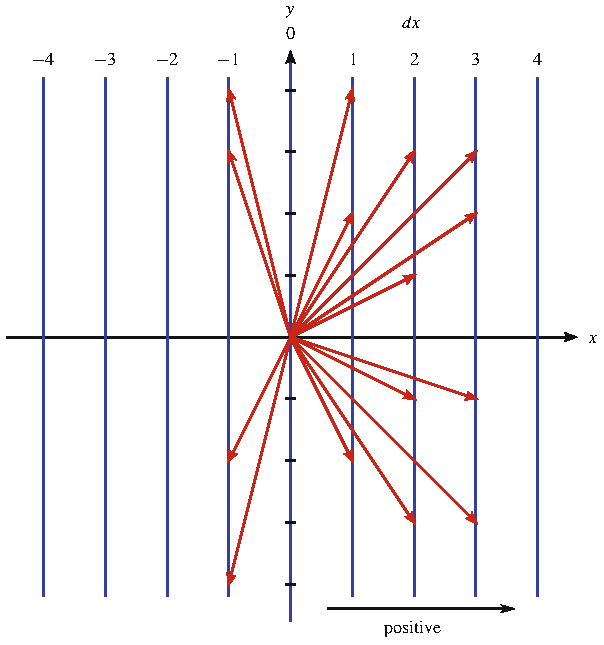
\includegraphics[width=0.716\linewidth]{images/vector/fig-5-1.pdf}
  \caption{使一形式 $dx$ 给出输出 $-1$、$1$、$2$ 和 $3$ 的向量. 图中显示了正方向}
  \label{fig:5-1}
\end{figure}

除了把 $dx$ 想成直线族 $x=\pm n$ 之外，我们还必须附上一个定向. 这在图中以指向右方的箭头显示，表示正定向. 于是向量 $\binom{-1}{4}$、$\binom{-1}{3}$ 与 $\binom{-1}{-2}$ 都刺穿一条直线，即直线 $x=-1$. 但由于这些向量是"向后"（沿负方向）走的，我们把它看作"刺穿负一次". 如果我们想考虑微分一形式 $-dx$，我们会得到同样的图，即由 $x=\pm n$ 给出的直线，但我们要把定向画在相反的方向.

现在考虑下面这些，
\begin{align*}
dx\binom{1.42}{4}=1.42,\quad dx\binom{1.97}{2}=1.97,\quad dx\binom{1.1}{-2}=1.1, \\
dx\binom{-1.21}{4}=-1.21,\quad dx\binom{-1.5}{3}=-1.5,\quad dx\binom{-1.92}{-2}=-1.92, \\
dx\binom{2.23}{5}=2.23,\quad dx\binom{2.74}{2}=2.74,\quad dx\binom{2.01}{-2}=2.01, \\
dx\binom{3.69}{6}=3.69,\quad dx\binom{3.91}{1}=3.91,\quad dx\binom{3.34}{-1}=3.34.
\end{align*}
显然 $dx\binom{1.42}{4}=1.42$ 是正确的，然而利用我们把 $dx$ 画成无穷序列直线 $x=\pm n$（$n=0,1,2,3,\ldots$）并附上定向的图像，向量 $\binom{1.42}{4.84}$ 只刺穿一条直线，即直线 $x=1$. 所以，利用关于 $dx$ 的"刺穿"图，我们有 $dx\binom{1.42}{4}=1$. 显然这不是精确的，但它的确给出一个近似. 利用这种刺穿的想法，我们会有
\begin{align*}
dx\binom{1.42}{4}=1,\quad dx\binom{1.97}{2}=1,\quad dx\binom{1.1}{-2}=1, \\
dx\binom{-1.21}{4}=-1,\quad dx\binom{-1.5}{3}=-1,\quad dx\binom{-1.92}{-2}=-1.
\end{align*}

以完全相同的方式，我们可以把微分形式 $dy_p\in T_p^*\mathbb{R}^2$ 表示成无穷序列的直线 $y=\pm n$（$n=0,1,2,3,\ldots$）连同定向，位于向量空间 $T_p\mathbb{R}^2$ 中. $dy_p(v_p)$ 的值是向量 $v_p$ 刺穿的直线的条数. 同样，如果向量的尖端碰到一条直线，即使它没有穿过这条直线，我们也认为它刺穿了这条直线.

\begin{figure}[htbp]
  \centering
  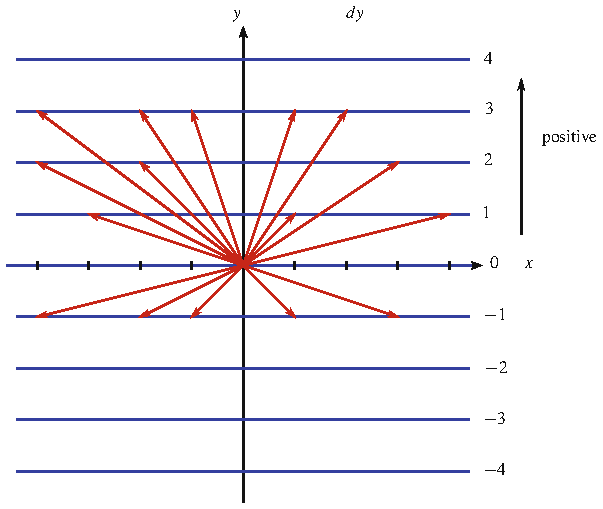
\includegraphics[width=0.715\linewidth]{images/vector/fig-5-2.pdf}
  \caption{使一形式 $dy$ 给出输出 $-1$、$1$、$2$ 和 $3$ 的向量. 图中显示了正方向}
  \label{fig:5-2}
\end{figure}

所以对于图~\ref{fig:5-2} 我们有
\begin{align*}
dy\binom{-2}{3}=3,\quad dy\binom{-2}{2}=2,\quad dy\binom{-3/2}{1}=1,\quad dy\binom{-2}{-1}=-1, \\
dy\binom{1}{3}=3,\quad dy\binom{1/2}{2}=2,\quad dy\binom{1}{1}=1,\quad dy\binom{-1}{-1}=-1, \\
dy\binom{4}{3}=3,\quad dy\binom{3}{2}=2,\quad dy\binom{3}{1}=1,\quad dy\binom{1}{-1}=-1.
\end{align*}
关于近似的上述评论同样适用. 例如，向量 $\binom{1.42}{4.84}$ 刺穿了我们的 $dy$ 图的四条直线，所以我们会得到 $dy\binom{1.42}{4.84}=4$，尽管精确值当然是 4.84.

但微分形式 $dx$ 与 $dy$ 并不是 $T_p^*\mathbb{R}^2$ 仅有的元素. 微分形式 $2dx_p\in T_p^*\mathbb{R}^2$ 在向量空间 $T_p\mathbb{R}^2$ 中会如何表示呢？考虑上面相同的向量，我们有
\begin{align*}
2dx\binom{1}{4}=2,\quad 2dx\binom{-1}{4}=-2,\quad 2dx\binom{2}{5}=4,\quad 2dx\binom{3}{6}=6, \\
2dx\binom{1}{2}=2,\quad 2dx\binom{-1}{3}=-2,\quad 2dx\binom{2}{2}=4,\quad 2dx\binom{3}{1}=6, \\
2dx\binom{1}{-2}=2,\quad 2dx\binom{-1}{-2}=-2,\quad 2dx\binom{2}{-2}=4,\quad 2dx\binom{3}{-1}=6.
\end{align*}

所以这些向量在 $2dx$ 的情形下刺穿的直线条数是 $dx$ 情形下的两倍，这意味着 $2dx$ 情形下直线的"密度"是 $dx$ 情形下直线的两倍. 我们会把它画成图~\ref{fig:5-3} 那样.

\begin{figure}[htbp]
  \centering
  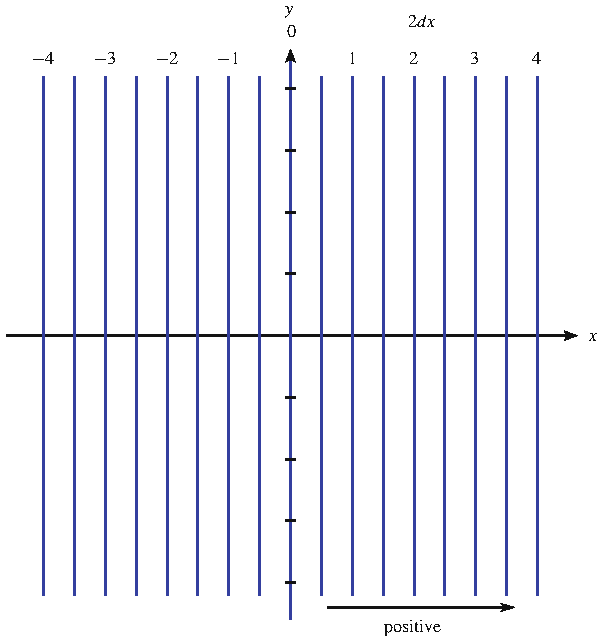
\includegraphics[width=0.716\linewidth]{images/vector/fig-5-3.pdf}
  \caption{用待刺穿的直线表示的一形式 $2dx$}
  \label{fig:5-3}
\end{figure}

我们可以在 $2dy$ 的情形下进行完全相同的分析. 同样，利用上面的相同向量，我们有
\begin{align*}
2dy\binom{-2}{3}=6,\quad 2dy\binom{-2}{2}=4,\quad 2dy\binom{-3/2}{1}=2,\quad 2dy\binom{-2}{-1}=-2, \\
2dy\binom{1}{3}=6,\quad 2dy\binom{1/2}{2}=4,\quad 2dy\binom{1}{1}=2,\quad 2dy\binom{-1}{-1}=-2, \\
2dy\binom{4}{3}=6,\quad 2dy\binom{3}{2}=4,\quad 2dy\binom{3}{1}=2,\quad 2dy\binom{1}{-1}=-2.
\end{align*}

同样，这些向量在 $2dy$ 的情形下刺穿的直线条数是 $dy$ 情形下的两倍，所以 $2dy$ 情形下直线的"密度"也是 $dy$ 情形下直线密度的两倍. 我们会把它画成图~\ref{fig:5-4} 那样.

\begin{figure}[htbp]
  \centering
  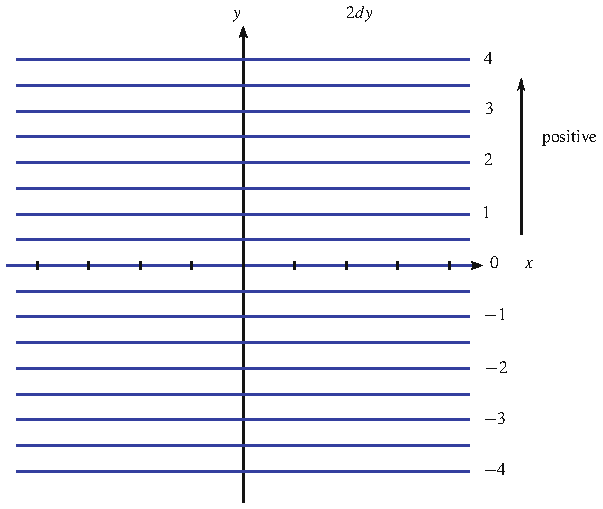
\includegraphics[width=0.715\linewidth]{images/vector/fig-5-4.pdf}
  \caption{用待刺穿的直线表示的一形式 $2dy$}
  \label{fig:5-4}
\end{figure}

显然，如果你对 $3dx$ 和 $3dy$ 做同样的分析，你会发现图形表示中直线的"密度"是 $dx$ 与 $dy$ 情形下的三倍，而对 $ndx$ 与 $ndy$ 则是 $n$ 倍.

\begin{question}\label{q:5-3}
画出表示下列微分形式的图：$3dx$、$5dy$、$\frac12dx$、$\frac23dx$、$\frac13dy$ 与 $\frac35dy$.
\end{question}

现在我们转向 $T_p^*\mathbb{R}^2$ 中更一般的元素. 我们从简单的东西 $dx+dy$ 开始. 考虑一形式 $dx+dy$ 如何作用在下列向量上，
\begin{align*}
(dx+dy)\binom{-1}{3}=-1+3=2,\qquad (dx+dy)\binom{1}{2}=1+2=3, \\
(dx+dy)\binom{-1}{1}=-1+1=0,\qquad (dx+dy)\binom{0}{1}=0+1=1, \\
(dx+dy)\binom{1}{1}=1+1=2,\qquad (dx+dy)\binom{-1}{0}=-1+0=-1, \\
(dx+dy)\binom{1}{0}=1+0=1,\qquad (dx+dy)\binom{0}{-1}=0-1=-1.
\end{align*}

图~\ref{fig:5-5} 是 $dx+dy$ 的一张可行的图. 它之所以可行，可以通过检查向量并数出它们刺穿了多少条直线（把所描绘的定向考虑进去）而看出来. 显然 $dx+dy$ 的图需要斜线. 通过检查可以明白，这些直线由 $y=-x+n$（$n=0,\pm1,\pm2,\ldots$）给出.

\begin{figure}[htbp]
  \centering
  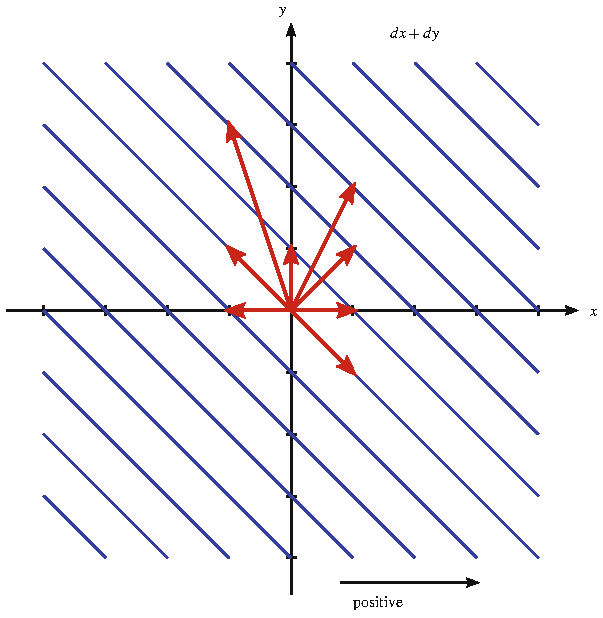
\includegraphics[width=0.715\linewidth]{images/vector/fig-5-5.pdf}
  \caption{一形式 $dx+dy$ 的待刺穿直线. 图中描绘了正方向}
  \label{fig:5-5}
\end{figure}

现在假设我们想画出微分一形式 $2dx+dy$、$dx-2dy$ 或更复杂的东西的图. 我们需要一种系统的方法来决定直线是什么. 这实际上相当容易. 考虑一形式 $2dx+dy$. 为了找到我们需要画出的直线来构成这个微分的图，我们只需从方程 $2x+y=n$（$n=0,\pm1,\pm2,\ldots$）开始，并解出 $y$，得到 $y=-2x+n$，如图~\ref{fig:5-6} 所示. 考虑图~\ref{fig:5-6} 中的向量 $v=\binom{1}{2}$. 它沿正方向"刺穿"了四条直线，所以根据图有 $(2dx+dy)(v)=4$. 计算上有
\[
(2dx+dy)\binom{1}{2}=2dx\binom{1}{2}+dy\binom{1}{2}=2(1)+2=4.
\]

类似地，为了画出一形式 $dx-2dy$ 的图，我们使用方程 $x-2y=n$，它变成 $y=\frac{x}{2}-\frac{n}{2}$. 见图~\ref{fig:5-7}.

\begin{figure}[htbp]
  \centering
  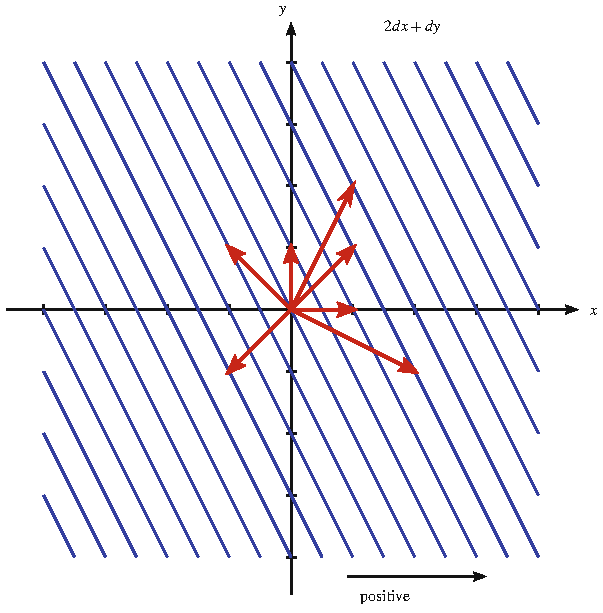
\includegraphics[width=0.715\linewidth]{images/vector/fig-5-6.pdf}
  \caption{一形式 $2dx+dy$ 的待刺穿直线. 图中描绘了正方向}
  \label{fig:5-6}
\end{figure}

\begin{figure}[htbp]
  \centering
  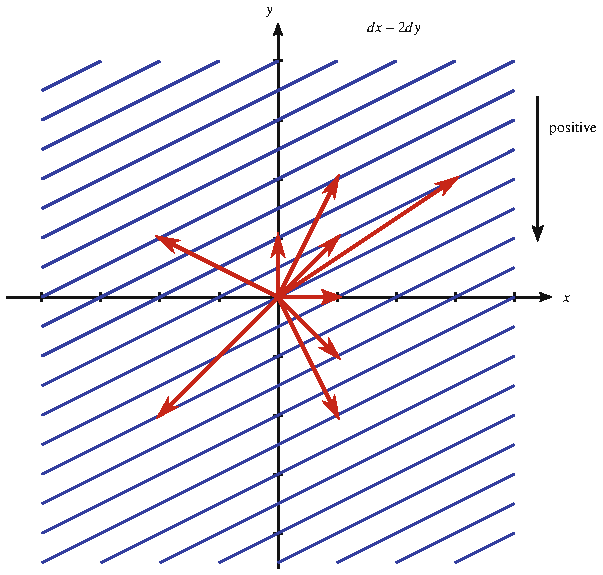
\includegraphics[width=0.742\linewidth]{images/vector/fig-5-7.pdf}
  \caption{一形式 $dx-2dy$ 的待刺穿直线. 图中描绘了正方向}
  \label{fig:5-7}
\end{figure}

\begin{question}\label{q:5-4}
检验在 $2dx+dy$ 与 $dx-2dy$ 的图中画出的各个向量，无论用计算还是用图形都给出相同的答案.
\end{question}

\begin{question}\label{q:5-5}
解释为什么上面寻找图形表示中直线的过程是可行的. 为此，考虑一般的一形式 $adx+bdy$ 如何作用在一般的向量 $v=\binom{x}{y}$ 上. 这个向量的哪些值给出 $(adx+bdy)(v)=n$（对任意 $n=0,\pm1,\pm2,\ldots$）？
\end{question}

\begin{question}\label{q:5-6}
画出下列微分形式的图形表示：
\begin{enumerate}
  \item[(a)] $3dx+dy$，
  \item[(b)] $2dx-dy$，
  \item[(c)] $-dx+3dy$.
\end{enumerate}
\end{question}

$T_p^*\mathbb{R}^2$ 中的微分一形式并不是唯一能作用在 $T_p\mathbb{R}^2$ 中向量上的形式. $\bigwedge_p^2(\mathbb{R}^2)$ 中的微分二形式也能作用在 $T_p\mathbb{R}^2$ 中的向量上. 如我们所知，微分二形式作用在 $T_p\mathbb{R}^2$ 中的两个向量上. 我们首先考虑向量
\[
v_1=\binom{1}{0},\qquad v_2=\binom{0}{1}
\]
以及微分二形式 $dx\wedge dy$. 我们有
\begin{align*}
(dx\wedge dy)(v_1,v_2)=
\begin{vmatrix}
dx(v_1) & dx(v_2)\\
dy(v_1) & dy(v_2)
\end{vmatrix}
=
\begin{vmatrix}
1 & 0\\
0 & 1
\end{vmatrix}
=1, \\
(dx\wedge dy)(v_2,v_1)=
\begin{vmatrix}
dx(v_2) & dx(v_1)\\
dy(v_2) & dy(v_1)
\end{vmatrix}
=
\begin{vmatrix}
0 & 1\\
1 & 0
\end{vmatrix}
=-1.
\end{align*}

和之前一样，我们想画一幅表示微分二形式 $dx\wedge dy$ 的 $T_p\mathbb{R}^2$ 中的图. 对微分一形式，我们使用由直线组成的图，然后数出我们的向量"刺穿"了多少条直线，从而得到该微分形式作用在向量上的近似值. 这里我们的图必须以某种方式把两个输入向量都考虑进去. 我们把 $T_p\mathbb{R}^2$ 中的微分二形式 $dx\wedge dy$ 表示为水平直线与竖直直线连同定向.

图~\ref{fig:5-8} 显示的是 $dx\wedge dy$ 的图，它由蓝色水平直线与绿色竖直直线组成，产生一个方形网格. 由向量 $v_1$ 与 $v_2$ 张成的平行六面体恰好覆盖网格的一个方格，因此我们说 $dx\wedge dy(v_1,v_2)$ 是 1. 现在我们只需要考虑定向. 由于 $(dx\wedge dy)(v_1,v_2)$ 是正的，我们用它来决定所需要的定向，这在图中被描绘为一个小圆形箭头，沿逆时针方向. 从 $v_1$ 到 $v_2$，沿着两个向量之间的最小角走过，是逆时针的，所以这就是被选择的定向. 因此，如果我们沿着第一个向量与第二个向量之间的最小角按逆时针方向走过，我们选择正；如果我们沿着第一个向量与第二个向量之间的最小角按顺时针方向走过，我们选择负. 所以对 $(dx\wedge dy)(v_2,v_1)$，第一个向量是 $v_2$，第二个向量是 $v_1$. 从第一个向量走到第二个向量，我们是沿顺时针方向走的，所以我们会选择负. 由向量 $v_2$ 与 $v_1$ 张成的平行六面体恰好覆盖一个方格，所以答案是 $-1$.

\begin{figure}[htbp]
  \centering
  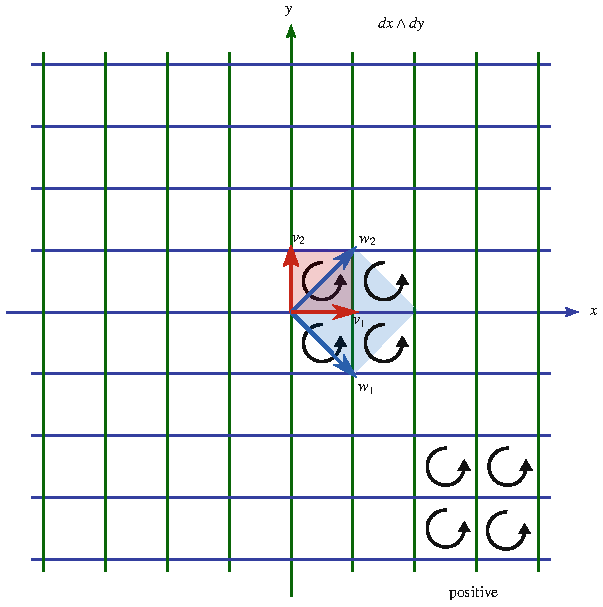
\includegraphics[width=0.715\linewidth]{images/vector/fig-5-8.pdf}
  \caption{二形式 $dx\wedge dy$ 由水平直线与竖直直线组成. 逆时针圆形箭头描绘了正方向}
  \label{fig:5-8}
\end{figure}

现在考虑向量
\[
w_1=\binom{1}{-1},\qquad w_2=\binom{1}{1}.
\]
计算上我们有
\begin{align*}
(dx\wedge dy)(w_1,w_2)=
\begin{vmatrix}
dx(w_1) & dx(w_2)\\
dy(w_1) & dy(w_2)
\end{vmatrix}
=
\begin{vmatrix}
1 & 1\\
-1 & 1
\end{vmatrix}
=2, \\
(dx\wedge dy)(w_2,w_1)=
\begin{vmatrix}
dx(w_2) & dx(w_1)\\
dy(w_2) & dy(w_1)
\end{vmatrix}
=
\begin{vmatrix}
1 & 1\\
1 & -1
\end{vmatrix}
=-2.
\end{align*}
利用图~\ref{fig:5-8} 可以看出，由 $w_1$ 与 $w_2$ 张成的平行六面体总共覆盖了两个网格方格，而如果我们沿最小角从 $w_1$ 走到 $w_2$，方向是逆时针的，所以我们选择正号，得到 $dx\wedge dy(w_1,w_2)=2$. 但如果我们沿最小角从 $w_2$ 走到 $w_1$，方向是顺时针的，所以我们选择负号，得到 $dx\wedge dy(w_2,w_1)=-2$.

现在我们转向微分二形式 $2dx\wedge dy$. 我们已经讨论过这种可视化微分形式的方式具有答案只是近似的缺点. 现在我们将说明另一个缺点. 对某些微分形式，我们使用什么样的图或图像可能有一些歧义. 我们再次考虑向量
\[
v_1=\binom{1}{0},\qquad v_2=\binom{0}{1},
\]
计算上它们给出
\[
(2dx\wedge dy)(v_1,v_2)=2
\begin{vmatrix}
1 & 0\\
0 & 1
\end{vmatrix}
=2.
\]
所以由 $v_1$ 与 $v_2$ 张成的平行六面体必须覆盖表示二形式 $2dx\wedge dy$ 的网格中的两个方框. 这样做的方式不是唯一的. 例如，对 $n=0,\pm1,\pm2,\ldots$ 选择直线 $y=n$ 与 $x=\frac{n}{2}$ 就能实现这一点；见图~\ref{fig:5-9}. 实现这一点的另一种方式是选择直线 $y=\frac{n}{2}$ 与 $x=n$（$n=0,\pm1,\pm2,\ldots$），如图~\ref{fig:5-10} 那样. 事实上，还有其他选择.

\begin{figure}[htbp]
  \centering
  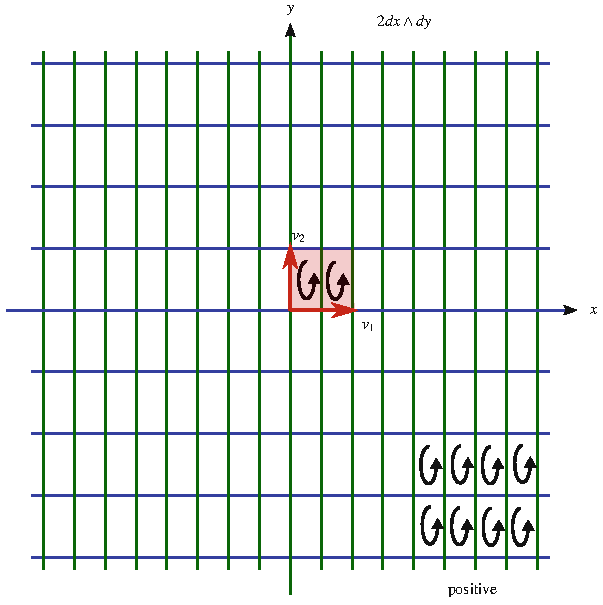
\includegraphics[width=0.715\linewidth]{images/vector/fig-5-9.pdf}
  \caption{画二形式 $2dx\wedge dy$ 的一种可行方式. 这里直线是 $x=n/2$ 与 $y=n$. 逆时针圆形箭头描绘了正方向}
  \label{fig:5-9}
\end{figure}

\begin{figure}[htbp]
  \centering
  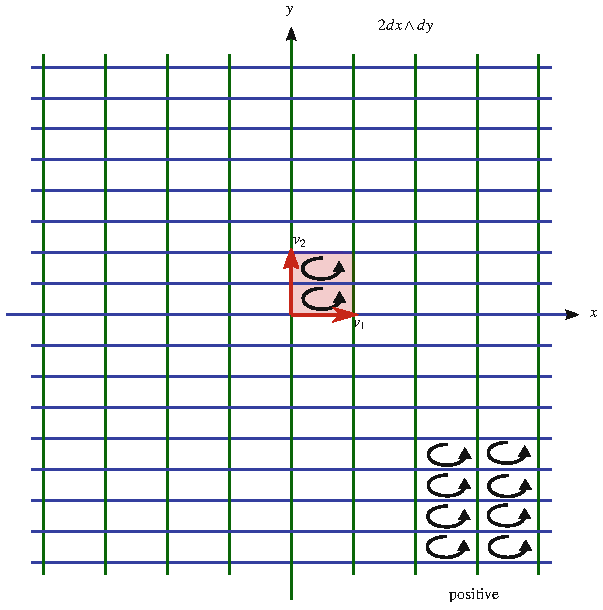
\includegraphics[width=0.715\linewidth]{images/vector/fig-5-10.pdf}
  \caption{画二形式 $2dx\wedge dy$ 的另一种可行方式. 这里直线是 $x=n$ 与 $y=n/2$. 逆时针圆形箭头描绘了正方向}
  \label{fig:5-10}
\end{figure}

\begin{question}\label{q:5-7}
为微分二形式 $2dx\wedge dy$ 找出另一种图形表示.
\end{question}

\begin{question}\label{q:5-8}
为下列每个微分二形式找出三种图形表示：
\begin{enumerate}
  \item[(a)] $3dx\wedge dy$，
  \item[(b)] $5dx\wedge dy$，
  \item[(c)] $\frac12dx\wedge dy$.
\end{enumerate}
\end{question}

\section{R³ 中的一形式}

和以前一样，我们固定流形 $\mathbb{R}^3$ 上的某一点 $p$，只考虑 $T_p^*\mathbb{R}^3$ 中的一形式. 我们将画出的一形式的"图"实际上叠加在向量空间 $T_p\mathbb{R}^3$ 上. 我们从一形式 $dx\in T_p^*\mathbb{R}^3$ 开始. 考虑 $dx$ 对下列向量的作用，
\begin{align*}
dx\begin{bmatrix}1\\0\\5\end{bmatrix}=1,\qquad
dx\begin{bmatrix}1\\0\\0\end{bmatrix}=1,\qquad
dx\begin{bmatrix}1\\2\\1\end{bmatrix}=1, \\
dx\begin{bmatrix}1\\2\\-1\end{bmatrix}=1,\qquad
dx\begin{bmatrix}1\\-3\\-2\end{bmatrix}=1,\qquad
dx\begin{bmatrix}1\\-4\\3\end{bmatrix}=1.
\end{align*}
任何终点落在 $T_p\mathbb{R}^3$ 中平面 $x=1$ 上的向量 $v\in T_p\mathbb{R}^3$ 都有值 1. 见图~\ref{fig:5-11}.

\begin{figure}[htbp]
  \centering
  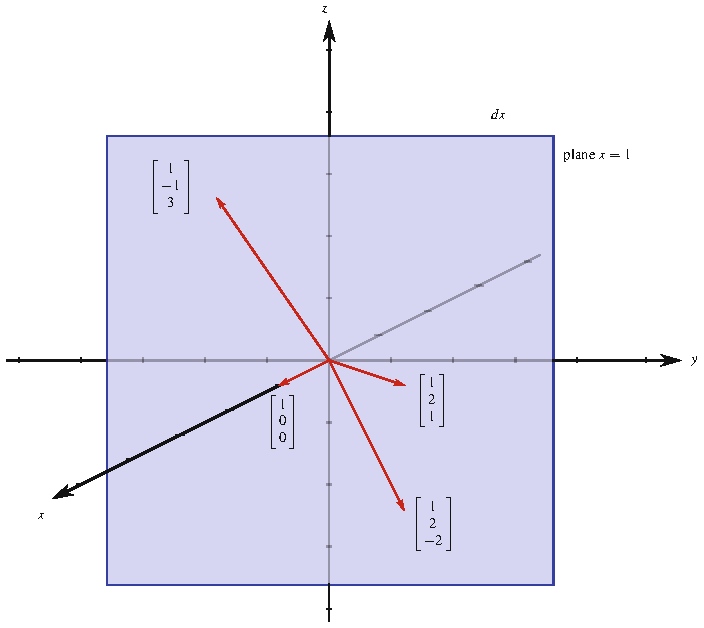
\includegraphics[width=0.891\linewidth]{images/vector/fig-5-11.pdf}
  \caption{$\mathbb{R}^3$ 中的平面 $x=1$. 一形式 $dx$ 把所有终点落在此平面上的向量送到值 1. 也就是说，若 $v$ 终点落在此平面上，则 $dx(v)=1$}
  \label{fig:5-11}
\end{figure}

类似地，考虑 $dx$ 对这些向量的作用，
\begin{align*}
dx\begin{bmatrix}3\\0\\0\end{bmatrix}=3,\qquad
dx\begin{bmatrix}2\\-2\\-1\end{bmatrix}=2,\qquad
dx\begin{bmatrix}0\\3\\4\end{bmatrix}=0, \\
dx\begin{bmatrix}3\\-1\\2\end{bmatrix}=3,\qquad
dx\begin{bmatrix}2\\-2\\-4\end{bmatrix}=2,\qquad
dx\begin{bmatrix}0\\-3\\-1\end{bmatrix}=0, \\
dx\begin{bmatrix}3\\2\\-5\end{bmatrix}=3,\qquad
dx\begin{bmatrix}2\\5\\-3\end{bmatrix}=2,\qquad
dx\begin{bmatrix}0\\-2\\5\end{bmatrix}=0.
\end{align*}

一形式把任何终点落在平面 $x=3$ 上的向量送到 $3$，把任何终点落在平面 $x=2$ 上的向量送到 $2$，把任何终点落在平面 $x=0$ 上的向量送到 $0$. 基于此，我们将在向量空间 $T_p\mathbb{R}^3$ 中把微分一形式 $dx\in T_p^*\mathbb{R}^3$ 图形化地表示为平面族 $x=n$，其中 $n=0,\pm1,\pm2,\ldots$. 在图~\ref{fig:5-12} 中，我们通过画出七个平面 $x=4$、$x=3$、$x=2$、$x=1$、$x=0$、$x=-1$ 与 $x=-2$ 来展示 $dx$.

\begin{figure}[htbp]
  \centering
  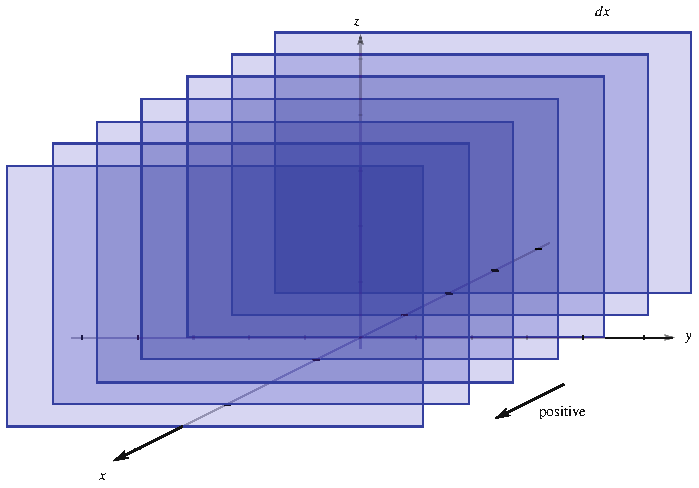
\includegraphics[width=0.863\linewidth]{images/vector/fig-5-12.pdf}
  \caption{在 $\mathbb{R}^3$ 中描绘为平面族的一形式 $dx$}
  \label{fig:5-12}
\end{figure}

利用这幅图我们说，向量 $v$ 的 $dx$ 就是 $v$ 所"刺穿"的平面的个数. 和以前一样，这样给出的答案只是近似答案. 例如，向量
\[
v_1=\begin{bmatrix}1\\-1\\7\end{bmatrix},\qquad
v_2=\begin{bmatrix}1.4\\1\\-2\end{bmatrix},\qquad
v_3=\begin{bmatrix}1.999\\-2\\5\end{bmatrix}
\]
都只刺穿一个平面，所以我们会说它们都有相同的值 $1$，尽管真正的答案显然是 $dx(v_1)=1$、$dx(v_2)=1.4$ 与 $dx(v_3)=1.999$. 同样，需要给这幅图赋予一个定向.

类似的推理得出，$dy$ 被图形化地表示为平面族 $y=n$，其中 $n=0,\pm1,\pm2,\ldots$，见图~\ref{fig:5-13}；而 $dz$ 被图形化地表示为平面族 $z=n$，其中 $n=0,\pm1,\pm2,\ldots$，见图~\ref{fig:5-14}.

\begin{figure}[htbp]
  \centering
  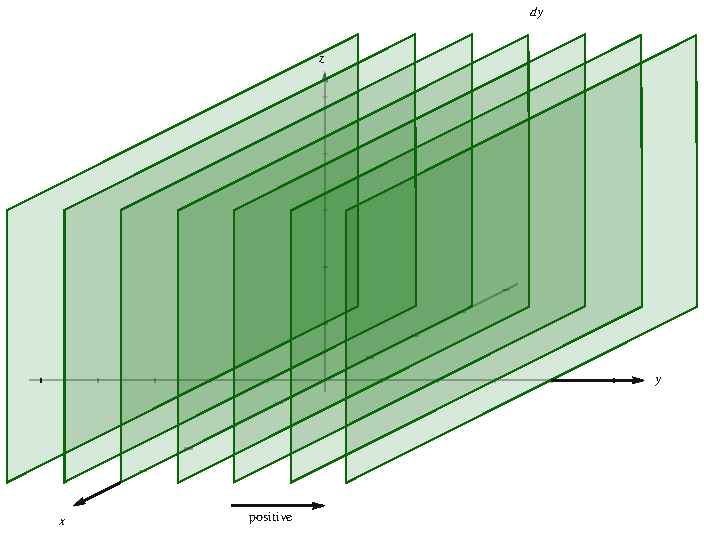
\includegraphics[width=0.947\linewidth]{images/vector/fig-5-13.pdf}
  \caption{在 $\mathbb{R}^3$ 中描绘为平面族的一形式 $dy$}
  \label{fig:5-13}
\end{figure}

\begin{figure}[htbp]
  \centering
  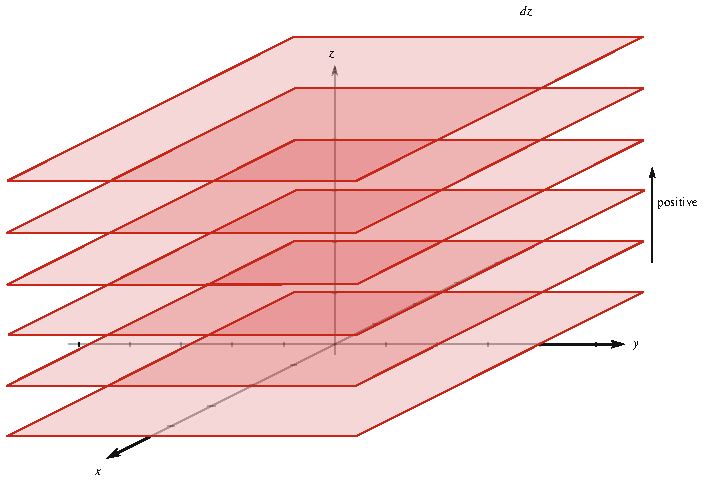
\includegraphics[width=0.960\linewidth]{images/vector/fig-5-14.pdf}
  \caption{在 $\mathbb{R}^3$ 中描绘为平面族的一形式 $dz$}
  \label{fig:5-14}
\end{figure}

\begin{question}\label{q:5-9}
证明图~\ref{fig:5-12}、图~\ref{fig:5-13} 与图~\ref{fig:5-14} 中描绘的正定向是正确的.
\end{question}

让我们花一点时间，把我们作为余切空间 $T_p^*\mathbb{R}^3$ 元素看待微分一形式的方式，与我们在 $T_p\mathbb{R}^3$ 上可视化微分形式的方式作一比较. 见图~\ref{fig:5-15}. $T_p^*\mathbb{R}^3$ 中的微分一形式也被称为余向量，它在余切空间中的画法与向量在切空间中的画法完全一样. 例如，一形式 $dx$ 是沿 $dx$ 轴的单位向量，一形式 $dy$ 是沿 $dy$ 轴的单位向量，一形式 $dz$ 是沿 $dz$ 轴的单位向量. 回忆我们选择总把余向量写成行向量，因此在 $T_p^*\mathbb{R}^3$ 中有 $dx=[1,0,0]$、$dy=[0,1,0]$、$dz=[0,0,1]$，所以一形式 $dx+dy+dz=[1,1,1]$. 在图~\ref{fig:5-15} 的上部，我们分别用蓝色、绿色与红色显示余向量 $dx$、$dy$ 与 $dz$.

\begin{figure}[htbp]
  \centering
  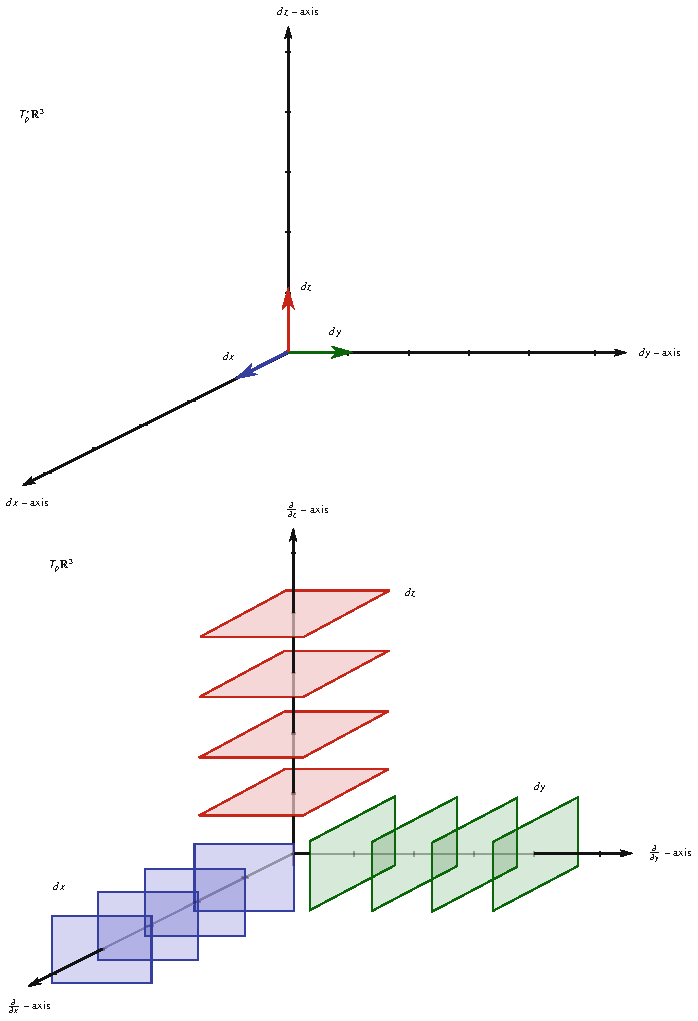
\includegraphics[width=0.852\linewidth]{images/vector/fig-5-15.pdf}
  \caption{一形式 $dx$（蓝）、$dy$（绿）与 $dz$（红）：上部在 $T_p^*\mathbb{R}^3$ 中描绘为余向量，下部在 $T_p\mathbb{R}^3$ 中描绘为平面}
  \label{fig:5-15}
\end{figure}

利用我们在本章引入的可视化微分形式的方法，微分一形式 $dx$ 被看成 $T_p\mathbb{R}^3$ 中垂直于 $\frac{\partial}{\partial x}$ 轴（也记为 $\frac{\partial}{\partial x}$ 轴）的无穷多个平面. 同样，微分一形式 $dy$ 是垂直于 $\frac{\partial}{\partial y}$ 轴的无穷多个平面，$dz$ 是垂直于 $\frac{\partial}{\partial z}$ 轴的无穷多个平面. 在图~\ref{fig:5-15} 的下部，我们分别用蓝色、绿色与红色显示了 $dx$、$dy$ 与 $dz$ 的少数几个平面.

与一形式 $dx$、$dy$、$dz$ 一样，一般的一形式 $adx+bdy+cdz$（其中 $a,b,c\in\mathbb{R}$）也可以被可视化为一族无穷多个平面. 作为例子，我们考虑一形式 $dx+dy$. 本质上，我们想以某种方式把 $dx$ 平面与 $dy$ 平面相加. 见图~\ref{fig:5-16}. 本质上，$dx$ 的平面垂直于向量
\[
\begin{bmatrix}1\\0\\0\end{bmatrix}
\]
而 $dy$ 的平面垂直于向量
\[
\begin{bmatrix}0\\1\\0\end{bmatrix}
\]
所以 $dx$ 与 $dy$ 的和，即 $dx+dy$，将是垂直于这两个向量之和的平面，也就是说，$dx+dy$ 的平面垂直于向量
\[
\begin{bmatrix}1\\1\\0\end{bmatrix}.
\]
答案显示在图~\ref{fig:5-17} 中.

\begin{figure}[htbp]
  \centering
  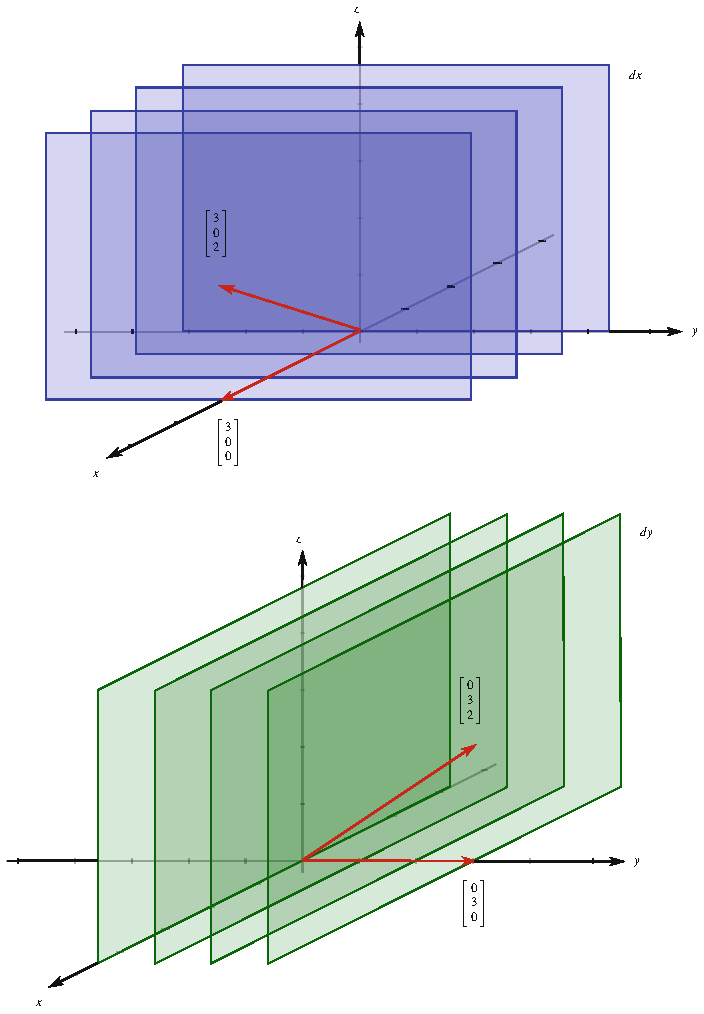
\includegraphics[width=0.865\linewidth]{images/vector/fig-5-16.pdf}
  \caption{为了找到 $dx+dy$ 的图形，我们想要以某种方式把 $dx$ 的平面（上）与 $dy$ 的平面（下）"相加". 这种"相加"给出图~\ref{fig:5-17} 中描绘的平面}
  \label{fig:5-16}
\end{figure}

\begin{figure}[htbp]
  \centering
  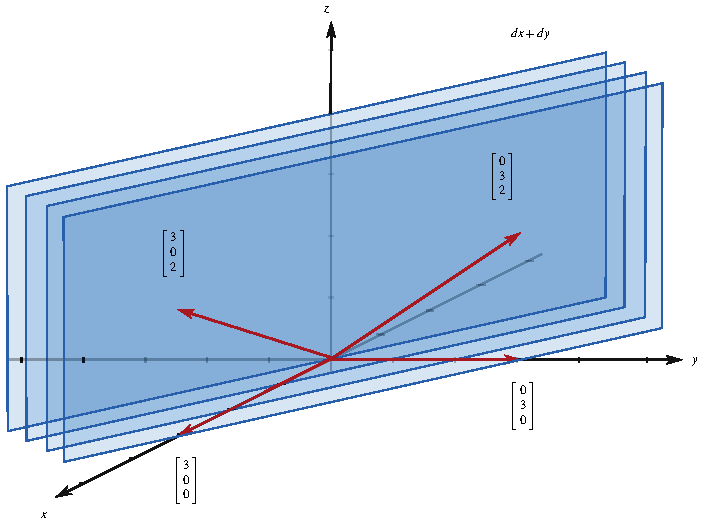
\includegraphics[width=0.960\linewidth]{images/vector/fig-5-17.pdf}
  \caption{描绘一形式 $dx+dy$ 的平面}
  \label{fig:5-17}
\end{figure}

Misner、Thorne 和 Wheeler 的书 \textit{Gravitation} 描述了寻找与 $dx+dy$ 相联系的平面的图形方法：选择适当的向量（比如下一个问题中的 $v_1$、$v_2$、$w_1$、$w_2$），数出它们刺穿的平面个数，然后用这些向量的端点来确定 $dx+dy$ 的一个平面. 下面几个问题将引导你走完他们的过程.

\begin{question}\label{q:5-10}
考虑向量
\[
v_1=\begin{bmatrix}3\\0\\0\end{bmatrix},\qquad
v_2=\begin{bmatrix}3\\0\\2\end{bmatrix},\qquad
w_1=\begin{bmatrix}0\\3\\0\end{bmatrix},\qquad
w_2=\begin{bmatrix}0\\3\\2\end{bmatrix}
\]
它们显示在图~\ref{fig:5-16} 中.
\begin{enumerate}
  \item[(a)] 分别用计算与图形从上面的图求出 $dx(v_1)$、$dx(v_2)$、$dx(w_1)$ 与 $dx(w_2)$.
  \item[(b)] 分别用计算与图形从上面的图求出 $dy(v_1)$、$dy(v_2)$、$dy(w_1)$ 与 $dy(w_2)$.
  \item[(c)] 分别用计算与图形从上面的图求出 $(dx+dy)(v_1)$、$(dx+dy)(v_2)$、$(dx+dy)(w_1)$ 与 $(dx+dy)(w_2)$.
  \item[(d)] $v_1$ 与 $v_2$ 刺穿了多少个 $dx$ 平面？多少个 $dy$ 平面？$w_1$ 与 $w_2$ 刺穿了多少个 $dy$ 平面？多少个 $dx$ 平面？那么这些向量中的每一个又刺穿多少个 $dx+dy$ 平面？
  \item[(e)] 基于 (a)--(d)，确定你将如何用向量 $v_1$、$v_2$、$w_1$、$w_2$ 来寻找 $dx+dy$ 的平面.
\end{enumerate}
\end{question}

\begin{question}\label{q:5-11}
在 $\mathbb{R}^3$ 上画出微分一形式 $dy+dz$ 与 $dx+dz$ 的草图.
\end{question}

现在我们有了比较 $dx+dy+dz$ 在 $T_p^*\mathbb{R}^3$ 中的表示与我们正在 $T_p\mathbb{R}^3$ 中可视化这一相同微分形式的方式所必需的全部构件，如图~\ref{fig:5-18} 那样.

\begin{figure}[htbp]
  \centering
  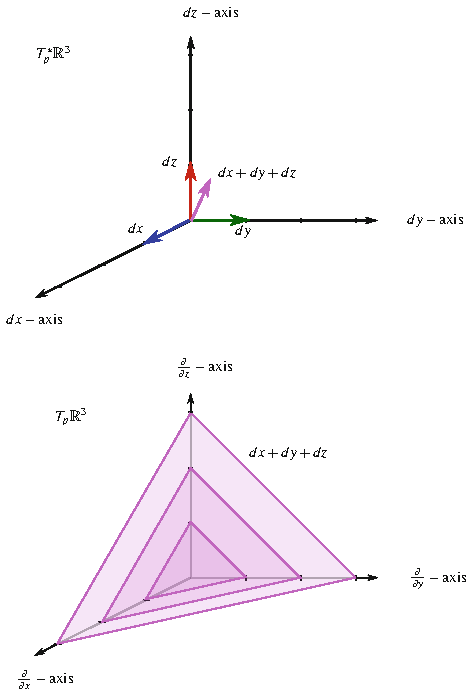
\includegraphics[width=0.573\linewidth]{images/vector/fig-5-18.pdf}
  \caption{一形式 $dx+dy+dz$：上部作为 $T_p^*\mathbb{R}^3$ 中的余向量，下部为在 $T_p\mathbb{R}^3$ 中描绘 $dx+dy+dz$ 的平面}
  \label{fig:5-18}
\end{figure}

\section{R³ 中的二形式}

类似于我们在 $T_p\mathbb{R}^2$ 中画二形式的方式，我们可以在 $T_p\mathbb{R}^3$ 中画二形式. 事实上，我们在 $T_p\mathbb{R}^3$ 中对二形式的图形表示本质上将是二维情形中网格线的三维版本. 我们不再尝试一步步走过这些图的推导过程，而是直接给出二形式 $dx\wedge dy$、$dy\wedge dz$ 与 $dz\wedge dx$ 的图，并说明它们是如何工作的. 我们从图~\ref{fig:5-19} 中二形式 $dx\wedge dy$ 的图开始.

\begin{figure}[htbp]
  \centering
  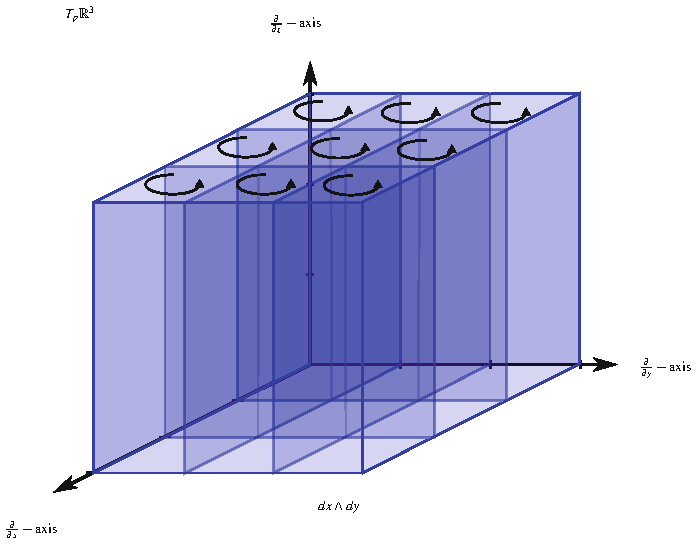
\includegraphics[width=0.960\linewidth]{images/vector/fig-5-19.pdf}
  \caption{在 $T_p\mathbb{R}^3$ 中描绘为一系列"管子"的二形式 $dx\wedge dy$，这些管子由平行于 $\frac{\partial}{\partial x}$ 轴与 $\frac{\partial}{\partial y}$ 轴的平面组成. 图中说明了正方向}
  \label{fig:5-19}
\end{figure}

注意，从图形上看，$dx\wedge dy$ 只不过就是同时画出 $dx$ 与 $dy$ 的平面，结果得到沿 $\frac{\partial}{\partial z}$ 方向延伸的"管子". 定向由管子中的小圆形箭头描绘. 俯视图上看，这些箭头沿逆时针方向转动. 我们不试图证明这是正确的图，而是用几个例子说明它是可行的. 首先考虑向量
\[
u_1=\begin{bmatrix}3\\0\\0\end{bmatrix}\qquad\text{与}\qquad u_2=\begin{bmatrix}0\\3\\0\end{bmatrix}.
\]
我们有
\[
(dx\wedge dy)(u_1,u_2)=
\begin{vmatrix}
3 & 0\\
0 & 3
\end{vmatrix}
=9.
\]
通过想象把向量 $u_1$ 与 $u_2$ 叠加到图~\ref{fig:5-19} 上，你可以看到由它们张成的平行六面体有九个 $dx\wedge dy$ 的"管子"穿过. 而且，当我们沿两个向量之间的最小角从 $u_1$ 走到 $u_2$ 时，我们移动的方向与施加在管子上的定向一致，所以这个 9 是正的. 如果我们沿两个向量之间的最小角从 $u_2$ 走到 $u_1$，那么我们移动的方向与施加在管子上的定向相反，所以在这种情形下 9 是负的，正如我们从计算
\[
(dx\wedge dy)(u_2,u_1)=
\begin{vmatrix}
0 & 3\\
3 & 0
\end{vmatrix}
=-9
\]
所预期的那样.

现在想象向量
\[
v_1=\begin{bmatrix}3\\0\\0\end{bmatrix}\qquad\text{与}\qquad v_2=\begin{bmatrix}0\\0\\3\end{bmatrix}
\]
叠加到图~\ref{fig:5-19} 上. 由这两个向量张成的平行六面体与管子平行，因而不穿过任何管子，所以在图形上我们有 $dx\wedge dy(v_1,v_2)=0$. 计算上我们得到相同的结果：
\[
(dx\wedge dy)(v_1,v_2)=
\begin{vmatrix}
3 & 0\\
0 & 0
\end{vmatrix}
=0.
\]

最后，想象向量
\[
w_1=\begin{bmatrix}0\\3\\0\end{bmatrix}\qquad\text{与}\qquad w_2=\begin{bmatrix}0\\0\\3\end{bmatrix}
\]
叠加到图~\ref{fig:5-19} 上. 同样，由 $w_1$ 与 $w_2$ 张成的平行六面体与管子平行，因而不穿过其中任何一根，给出 $dx\wedge dy(w_1,w_2)=0$，这同样与计算
\[
(dx\wedge dy)(w_1,w_2)=
\begin{vmatrix}
0 & 0\\
3 & 0
\end{vmatrix}
=0
\]
相符.

$dy\wedge dz$ 的图形表示与 $dx\wedge dy$ 非常相似，基本上由 $dy$ 与 $dz$ 的平面组成，得到平行于 $\frac{\partial}{\partial x}$ 轴的管子，如图~\ref{fig:5-20} 那样. 我们再次考虑由 $u_1$ 与 $u_2$、$v_1$ 与 $v_2$、$w_1$ 与 $w_2$ 张成的平行六面体与多少根管子相交. 计算上我们有
\begin{align*}
(dy\wedge dz)(u_1,u_2)=
\begin{vmatrix}
0 & 3\\
0 & 0
\end{vmatrix}
=0, \\
(dy\wedge dz)(v_1,v_2)=
\begin{vmatrix}
0 & 0\\
0 & 3
\end{vmatrix}
=0, \\
(dy\wedge dz)(w_1,w_2)=
\begin{vmatrix}
3 & 0\\
0 & 3
\end{vmatrix}
=9.
\end{align*}

\begin{figure}[htbp]
  \centering
  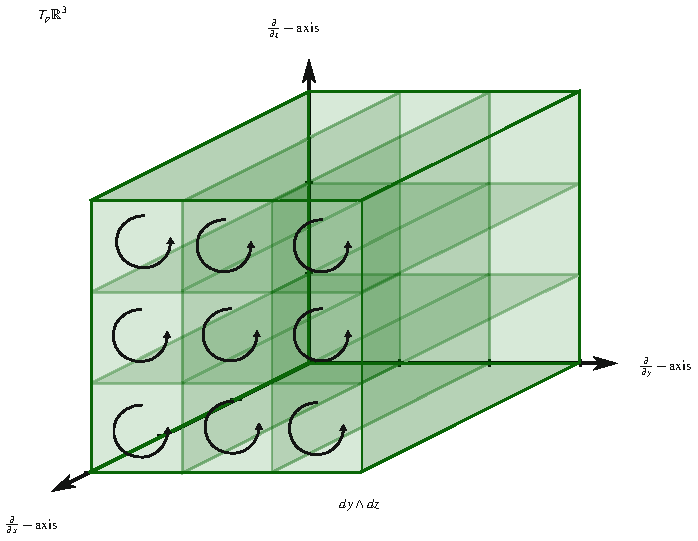
\includegraphics[width=0.960\linewidth]{images/vector/fig-5-20.pdf}
  \caption{在 $T_p\mathbb{R}^3$ 中描绘为一系列"管子"的二形式 $dy\wedge dz$，这些管子由平行于 $\frac{\partial}{\partial y}$ 轴与 $\frac{\partial}{\partial z}$ 轴的平面组成. 图中说明了正方向}
  \label{fig:5-20}
\end{figure}

通过想象把向量 $u_1$ 与 $u_2$ 叠加到 $dy\wedge dz$ 的图上，我们可以看到由这两个向量张成的平行六面体与管子平行，因而不穿过其中任何一根. 类似地，由 $v_1$ 与 $v_2$ 张成的平行六面体不穿过任何管子，但由 $w_1$ 与 $w_2$ 张成的平行六面体穿过九根管子.

最后，$dz\wedge dx$ 的图形表示由 $dz$ 与 $dx$ 的平面组成，得到平行于 $\frac{\partial}{\partial y}$ 轴的管子. 见图~\ref{fig:5-21}. 用上面的向量做类似的分析会得到预期的结果.

\begin{figure}[htbp]
  \centering
  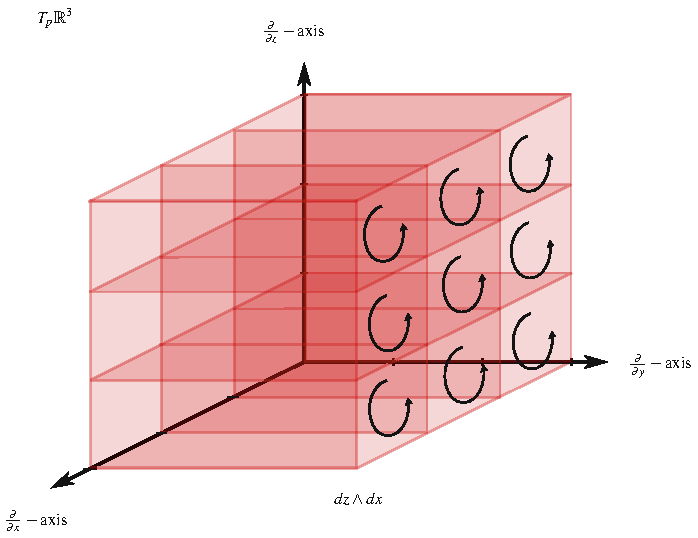
\includegraphics[width=0.887\linewidth]{images/vector/fig-5-21.pdf}
  \caption{在 $T_p\mathbb{R}^3$ 中描绘为一系列"管子"的二形式 $dz\wedge dx$，这些管子由平行于 $\frac{\partial}{\partial z}$ 轴与 $\frac{\partial}{\partial x}$ 轴的平面组成. 图中说明了正方向}
  \label{fig:5-21}
\end{figure}

当为二形式 $adx\wedge dy$、$bdy\wedge dz$、$cdz\wedge dx$（其中 $a,b,c\in\mathbb{R}$）寻找图形表示时，我们有与二维情形完全相同的歧义.

\begin{question}\label{q:5-12}
为微分二形式 $4dx\wedge dy$ 找出至少三种不同的图形表示.
\end{question}

现在我们考虑一般的微分二形式 $adx\wedge dy+bdy\wedge dz+cdz\wedge dx$，其中 $a,b,c\in\mathbb{R}$. 为简单起见，我们首先考虑二形式 $dx\wedge dy+dy\wedge dz$. 本质上，我们想找到这两幅图之和的图形表示，见图~\ref{fig:5-22}. 微分二形式 $dx\wedge dy$ 的管子平行于 $\frac{\partial}{\partial z}$ 轴，微分二形式 $dy\wedge dz$ 的管子平行于 $\frac{\partial}{\partial x}$ 轴. 考虑 $\frac{\partial}{\partial x}$ 方向的单位向量与 $\frac{\partial}{\partial z}$ 方向的单位向量. 把这两个单位向量相加，我们得到
\[
\begin{bmatrix}1\\0\\0\end{bmatrix}+\begin{bmatrix}0\\0\\1\end{bmatrix}=\begin{bmatrix}1\\0\\1\end{bmatrix}.
\]
$dx\wedge dy+dy\wedge dz$ 的管子平行于由这个向量确定的直线，如图~\ref{fig:5-23} 所示.

\begin{figure}[htbp]
  \centering
  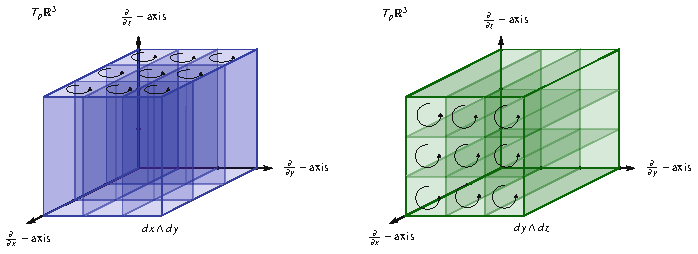
\includegraphics[width=0.960\linewidth]{images/vector/fig-5-22.pdf}
  \caption{为了找到二形式 $dx\wedge dy+dy\wedge dz$ 的图形表示，我们必须以某种方式把 $dx\wedge dy$（左）的管子与 $dy\wedge dz$（右）的管子"相加". 这些管子的"相加"结果如图~\ref{fig:5-23} 所示}
  \label{fig:5-22}
\end{figure}

\begin{figure}[htbp]
  \centering
  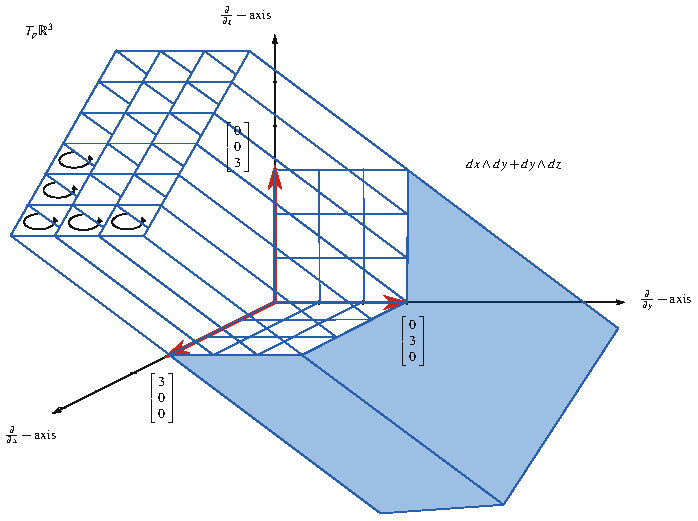
\includegraphics[width=0.940\linewidth]{images/vector/fig-5-23.pdf}
  \caption{把图~\ref{fig:5-22} 中 $dx\wedge dy$ 与 $dy\wedge dz$ 的管子"相加"所得的二形式 $dx\wedge dy+dy\wedge dz$ 的图形表示}
  \label{fig:5-23}
\end{figure}

\begin{question}\label{q:5-13}
设
\[
u=\begin{bmatrix}3\\0\\0\end{bmatrix},\qquad
v=\begin{bmatrix}0\\3\\0\end{bmatrix},\qquad
w=\begin{bmatrix}0\\0\\3\end{bmatrix}.
\]
借助图~\ref{fig:5-23} 证明，对下列各式，图形给出的答案与计算给出的答案一致：
\begin{enumerate}
  \item[(a)] $(dx\wedge dy+dy\wedge dz)(u,v)$，
  \item[(b)] $(dx\wedge dy+dy\wedge dz)(v,w)$，
  \item[(c)] $(dx\wedge dy+dy\wedge dz)(w,u)$.
\end{enumerate}
\end{question}

直观上看，与 $dx\wedge dy+dy\wedge dz$ 相联系的图似乎是有道理的. 还有另一种方式来看正在发生的事情. 回忆用来描绘一形式 $dx$ 的平面垂直于 $x$（或 $\frac{\partial}{\partial x}$）轴，用来描绘 $dy$ 的平面垂直于 $y$（或 $\frac{\partial}{\partial y}$）轴. 然后我们通过同时描绘这两族平面找到了 $dx\wedge dy$ 的图像. 我们的目标是把二形式 $dx\wedge dy+dy\wedge dz$ 变形为一种允许我们做类似事情的形式，
\[
dx\wedge dy+dy\wedge dz=-dy\wedge dx+dy\wedge dz=dy\wedge(-dx+dz)=dy\wedge d(-x+z).
\]

\begin{figure}[htbp]
  \centering
  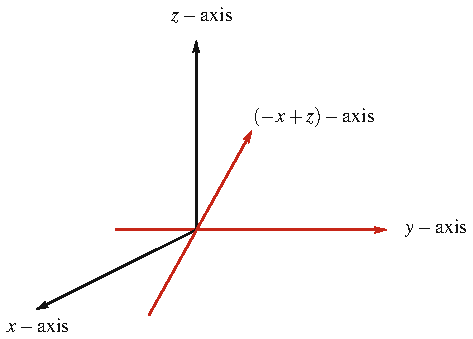
\includegraphics[width=0.561\linewidth]{images/vector/fig-5-24.pdf}
  \caption{垂直于 $y$ 轴与 $(-x+z)$ 轴的平面给出图~\ref{fig:5-23} 中所描绘的二形式 $dx\wedge dy+dy\wedge dz$}
  \label{fig:5-24}
\end{figure}

所以 $dx\wedge dy+dy\wedge dz$ 可以用垂直于 $y$ 轴与 $(-x+z)$"轴"的平面来表示. 最后这一点需要稍作解释. 考虑 $x$ 方向与 $z$ 方向的单位向量，把第一个的负向量加到第二个上，我们得到
\[
-\begin{bmatrix}1\\0\\0\end{bmatrix}+\begin{bmatrix}0\\0\\1\end{bmatrix}=\begin{bmatrix}-1\\0\\1\end{bmatrix}.
\]
向量 $\begin{bmatrix}-1\\0\\1\end{bmatrix}$ 确定了所使用的轴. 垂直于这个轴的平面是我们使用的第二族平面. 总之，对 $dx\wedge dy+dy\wedge dz$，使用的是垂直于图~\ref{fig:5-24} 中所画的两条红色轴的平面.

现在我们想找到 $dy\wedge dz+dz\wedge dx$ 的图，见图~\ref{fig:5-25}. 通过检查 $dy\wedge dz$ 与 $dz\wedge dx$ 的图可以看出，$dy\wedge dz+dz\wedge dx$ 的管子将平行于向量
\[
\begin{bmatrix}1\\1\\0\end{bmatrix}.
\]
或者我们也可以像前面那样改写 $dy\wedge dz+dz\wedge dx$，
\[
dy\wedge dz+dz\wedge dx=-dz\wedge dy+dz\wedge dx=dz\wedge(-dy+dx)=dz\wedge d(-y+x),
\]
并使用垂直于 $z$ 轴与 $(-y+x)$"轴"的平面，后者位于向量
\[
\begin{bmatrix}-1\\1\\0\end{bmatrix}
\]
的方向上. 这两个轴在图~\ref{fig:5-26} 中以红色显示.

\begin{figure}[htbp]
  \centering
  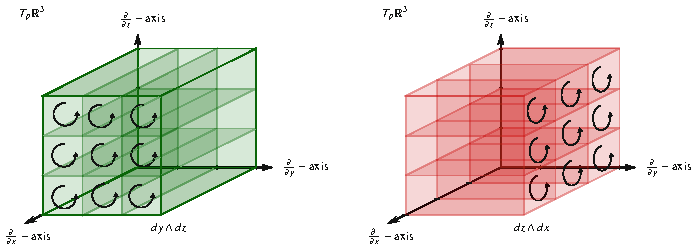
\includegraphics[width=0.960\linewidth]{images/vector/fig-5-25.pdf}
  \caption{为了找到二形式 $dy\wedge dz+dz\wedge dx$ 的图形表示，我们需要把 $dy\wedge dz$（左）与 $dz\wedge dx$（右）的管子"相加"}
  \label{fig:5-25}
\end{figure}

\begin{figure}[htbp]
  \centering
  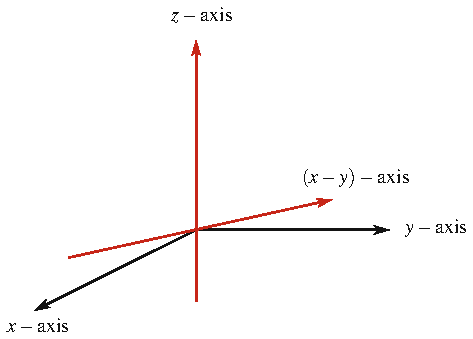
\includegraphics[width=0.561\linewidth]{images/vector/fig-5-26.pdf}
  \caption{$dy\wedge dz+dz\wedge dx$ 的管子由垂直于 $x$ 轴与 $(x-y)$ 轴的平面组成}
  \label{fig:5-26}
\end{figure}

现在我们想找到 $dx\wedge dy+dz\wedge dx$ 的图. 见图~\ref{fig:5-27}. 通过检查可以看出，$dx\wedge dy+dz\wedge dx$ 的管子平行于向量
\[
\begin{bmatrix}0\\1\\1\end{bmatrix},
\]
或者我们可以改写这个二形式，
\[
dx\wedge dy+dz\wedge dx=dx\wedge dy-dx\wedge dz=dx\wedge(dy-dz)=dx\wedge d(y-z)
\]
得到用来寻找垂直平面的两个轴. 这两个轴在图~\ref{fig:5-28} 中以红色显示.

\begin{figure}[htbp]
  \centering
  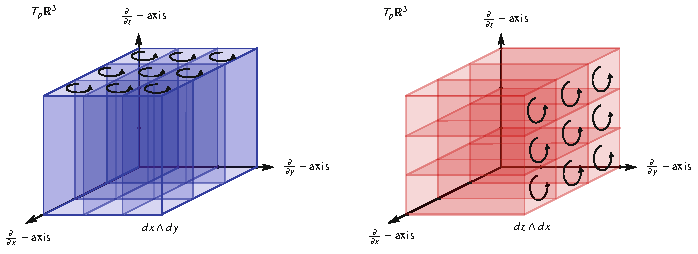
\includegraphics[width=0.960\linewidth]{images/vector/fig-5-27.pdf}
  \caption{二形式 $dx\wedge dy+dz\wedge dx$ 由把 $dx\wedge dy$（左）的管子与 $dz\wedge dx$（右）的管子相加得到}
  \label{fig:5-27}
\end{figure}

\begin{figure}[htbp]
  \centering
  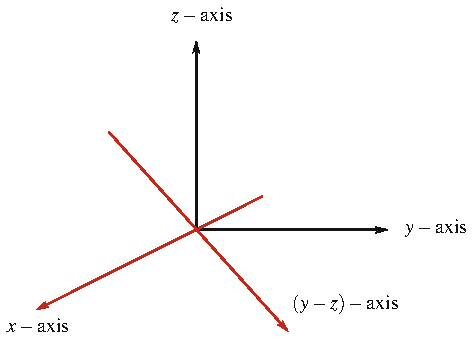
\includegraphics[width=0.561\linewidth]{images/vector/fig-5-28.pdf}
  \caption{二形式 $dx\wedge dy+dz\wedge dx$ 由垂直于 $x$ 轴与 $(y-z)$ 轴的平面组成}
  \label{fig:5-28}
\end{figure}

最后，我们想找到 $dx\wedge dy+dy\wedge dz+dz\wedge dx$ 的图. 见图~\ref{fig:5-29}. 我们可以如下改写二形式 $dx\wedge dy+dy\wedge dz+dz\wedge dx$，
\begin{align*}
dx\wedge dy+dy\wedge dz+dz\wedge dx=dy\wedge d(-x+z)+dz\wedge dx, \\
=dy\wedge d(-x+z)-dz\wedge(-dx)+dz\wedge dz, \\
=dy\wedge d(-x+z)-dz\wedge(-dx+dz), \\
=dy\wedge d(-x+z)-dz\wedge d(-x+z), \\
=(dy-dz)\wedge d(-x+z), \\
=d(y-z)\wedge d(-x+z),
\end{align*}
它可以用来勾画这个二形式. 最后，当转向带系数的二形式时，所有常见的问题都会出现.

\begin{figure}[htbp]
  \centering
  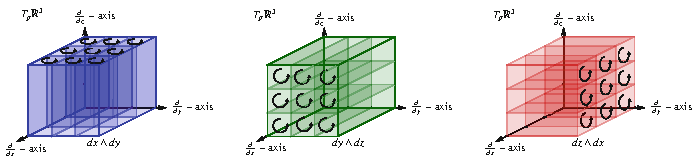
\includegraphics[width=0.960\linewidth]{images/vector/fig-5-29.pdf}
  \caption{二形式 $dx\wedge dy+dy\wedge dz+dz\wedge dx$ 由"相加"$dx\wedge dy$（左）、$dy\wedge dz$（中）与 $dz\wedge dx$（右）的管子得到}
  \label{fig:5-29}
\end{figure}

\begin{question}\label{q:5-14}
画出二形式 $dy\wedge dz+dz\wedge dx$ 的草图.
\end{question}

\begin{question}\label{q:5-15}
画出二形式 $dx\wedge dy+dz\wedge dx$ 的草图.
\end{question}

\begin{question}\label{q:5-16}
画出二形式 $dx\wedge dy+dy\wedge dz+dz\wedge dx$ 的草图.
\end{question}

\begin{question}\label{q:5-17}
画出下列每个二形式的一幅草图：
\begin{enumerate}
  \item[(a)] $2dx\wedge dy+dy\wedge dz$，
  \item[(b)] $dx\wedge dy+3dy\wedge dz$，
  \item[(c)] $2dx\wedge dy+4dy\wedge dz$.
\end{enumerate}
\end{question}

\begin{question}\label{q:5-18}
画出下列每个二形式的一幅草图：
\begin{enumerate}
  \item[(a)] $3dy\wedge dz+2dz\wedge dx$，
  \item[(b)] $dx\wedge dy+3dz\wedge dx$，
  \item[(c)] $2dx\wedge dy+4dy\wedge dz+3dz\wedge dx$.
\end{enumerate}
\end{question}

\begin{question}\label{q:5-19}
画出下列二形式的草图：
\begin{enumerate}
  \item[(a)] $-dx\wedge dy+dy\wedge dz$，
  \item[(b)] $dx\wedge dy-dy\wedge dz$，
  \item[(c)] $-dx\wedge dy-dy\wedge dz$.
\end{enumerate}
负号有什么影响？用一些精心选择的向量来帮助你弄清楚.
\end{question}

\section{R³ 中的三形式}

这很可能是整本书中最短的一节. 这是有原因的. 在 $T_p\mathbb{R}^3$ 中画三形式事实上极其简单. $\mathbb{R}^3$ 上的三形式空间，记为 $\bigwedge^3(\mathbb{R}^3)$，实际上是一维的，这意味着 $\mathbb{R}^3$ 上的每个三形式都有 $cdx\wedge dy\wedge dz$ 的形式，其中 $c\in\mathbb{R}$. 一形式 $dx$ 由平面 $x=n$ 给出，一形式 $dy$ 由平面 $y=n$ 给出，一形式 $dz$ 由平面 $z=n$ 给出，其中 $n=0,\pm1,\pm2,\ldots$. 三形式只不过就是同时画出所有这些平面，从而用单位立方体填满空间. 见图~\ref{fig:5-30}. 对于三形式 $adx\wedge dy\wedge dz$（其中 $a\in\mathbb{R}$），会出现常见的歧义.

\begin{figure}[htbp]
  \centering
  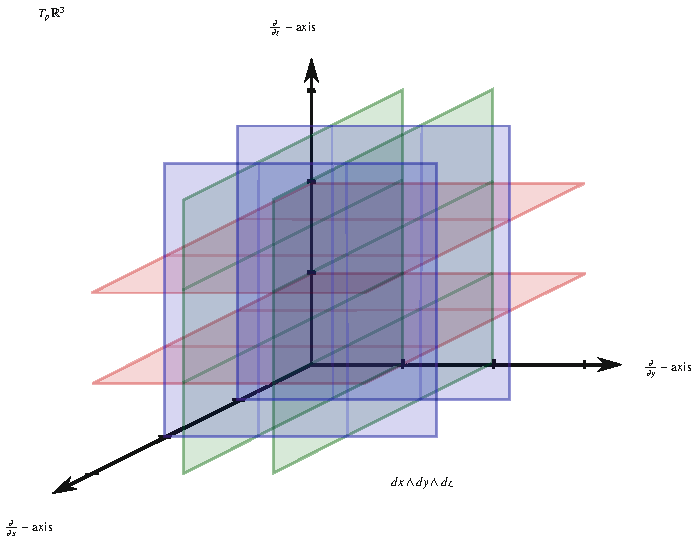
\includegraphics[width=0.960\linewidth]{images/vector/fig-5-30.pdf}
  \caption{三形式 $dx\wedge dy\wedge dz$ 由"立方体"组成，这些立方体的面是垂直于 $x$ 轴、$y$ 轴与 $z$ 轴的平面}
  \label{fig:5-30}
\end{figure}

\begin{question}\label{q:5-20}
基于图~\ref{fig:5-30}，为三形式 $2dx\wedge dy\wedge dz$ 画出三幅不同的草图.
\end{question}

\begin{question}\label{q:5-21}
设
\[
u=\begin{bmatrix}1\\0\\0\end{bmatrix},\qquad
v=\begin{bmatrix}0\\1\\0\end{bmatrix},\qquad
w=\begin{bmatrix}0\\0\\1\end{bmatrix}.
\]
在 $u$、$v$、$w$ 的不同排列上求值 $dx\wedge dy\wedge dz$，并用你的答案确定 $dx\wedge dy\wedge dz$ 具有什么样的定向. （注意，三个方向都必须以某种方式被考虑进去.）
\end{question}

\begin{question}\label{q:5-22}
你如何描绘图~\ref{fig:5-30} 中 $dx\wedge dy\wedge dz$ 的正定向？负定向呢？
\end{question}

\section{流形上形式的图形}

到目前为止我们一直在做的是，尝试画出 $\mathbb{R}^2$ 上的一形式与二形式以及 $\mathbb{R}^3$ 上的一形式、二形式与三形式的图形表示. 在每种情形下，我们都在点 $p$ 处考察某个形式 $\alpha_p$，并在点 $p$ 处的切空间中找到 $\alpha_p$ 的一个表示. 对 $\mathbb{R}^2$ 上的一形式，我们的图是 $T_p\mathbb{R}^2$ 中的直线（图~\ref{fig:5-1}--\ref{fig:5-7}）；而对 $\mathbb{R}^2$ 上的二形式，我们的图是 $T_p\mathbb{R}^2$ 中的方框（图~\ref{fig:5-8}--\ref{fig:5-10}）. 对 $\mathbb{R}^3$ 中的一形式，我们的图是 $T_p\mathbb{R}^3$ 中的平面（图~\ref{fig:5-11}--\ref{fig:5-18}）；对 $\mathbb{R}^3$ 中的二形式，我们的图是 $T_p\mathbb{R}^3$ 中的管子（图~\ref{fig:5-19}--\ref{fig:5-29}）；对 $\mathbb{R}^3$ 中的三形式，我们的图是 $T_p\mathbb{R}^3$ 中的立方体（图~\ref{fig:5-30}）.

有时人们会尝试利用这些 $\mathbb{R}^2$ 上的一形式与二形式以及 $\mathbb{R}^3$ 上的一形式、二形式与三形式的图形表示来"画出"整个流形上的形式，至少对二维或三维的流形是如此. 这通常有两种做法. 第一种方法至少在数学上说得通，尽管在某种意义上它仍可能是不完整的，并可能错误地表示微分形式. 不幸的是，第二种方法除可能错误地表示微分形式外，还有一些严重的数学缺陷. 但当这些方法确实可行时，它们可以成为思考二维与三维流形上微分形式的一种极其有用而富有启发的途径. 最好在脑海中记住，这些方法给出的图充其量只是漫画.

首先，我们介绍在流形上可视化形式的第一种方法. 这里所做的基本上是：在流形上选取一个点阵 $p_{ij}=(x_i,y_j)$，并在每个这样的阵点上把表示 $T_{p_{ij}}M$ 中一形式的线桩画在流形上. 图~\ref{fig:5-31} 显示了如何对 $\mathbb{R}^2$ 上一系列简单的一形式做到这一点. 箭头指向表示正方向. 当然，我们可以选择流形上密度不同的点阵. 图~\ref{fig:5-32} 用两种不同的点阵显示了 $\mathbb{R}^2$ 上相同的一形式 $xdx+ydy$. 二形式将类似，只是在每个点画一个小方框网格. 这种方法的缺点是点阵的间距；如果选择了不合适的点阵，完全有可能漏掉微分形式的重要细节. 尽管如此，人们通常仍会得到一个合理的漫画，它至少可以帮助人们想象这个微分形式.

\begin{figure}[htbp]
  \centering
  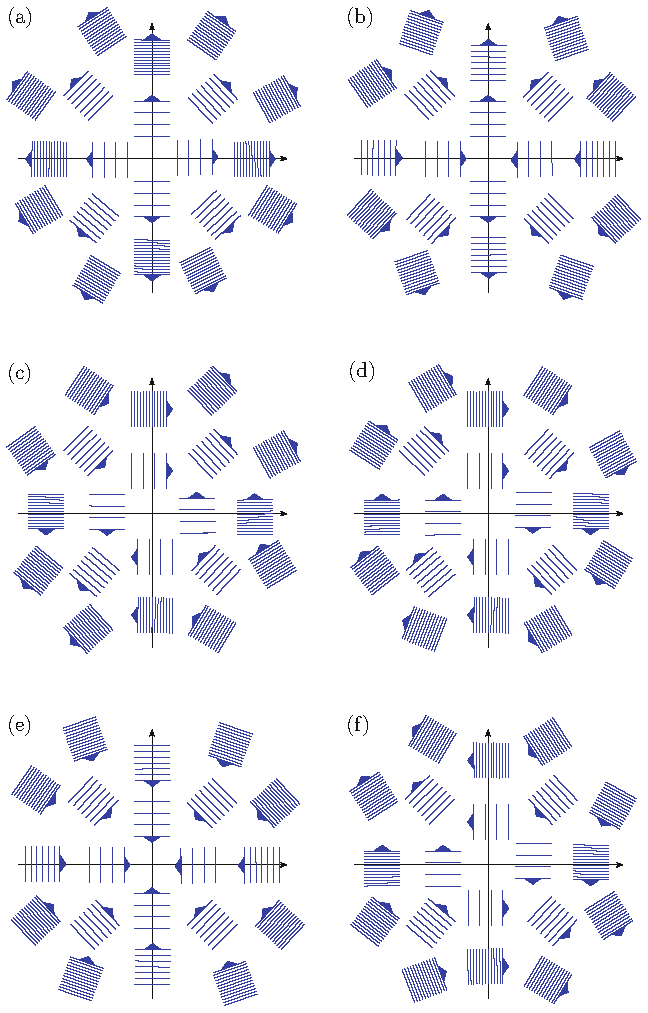
\includegraphics[width=0.768\linewidth]{images/vector/fig-5-31.pdf}
  \caption{流形 $\mathbb{R}^2$ 上的一形式，表示为流形 $\mathbb{R}^2$ 上的线桩网格. 箭头指向表示正方向（图像由 Vector Field Analyzer II, Version 2, Kawski, 2001 生成）. (a) $xdx+ydy$. (b) $-xdx+ydy$. (c) $ydx+xdy$. (d) $ydx-xdy$. (e) $-xdx-ydy$. (f) $-ydx-xdy$}
  \label{fig:5-31}
\end{figure}

对三维流形，图形是类似的. 首先在流形上选取一个三维点阵 $p_{ijk}=(x_i,y_j,z_k)$. 那么一形式将在每个点 $p_{ijk}$ 处表示为小的薄片桩，二形式将在每个点 $p_{ijk}$ 处表示为小的管子束，三形式将在每个点 $p_{ijk}$ 处表示为小的一组立方体.

\begin{figure}[htbp]
  \centering
  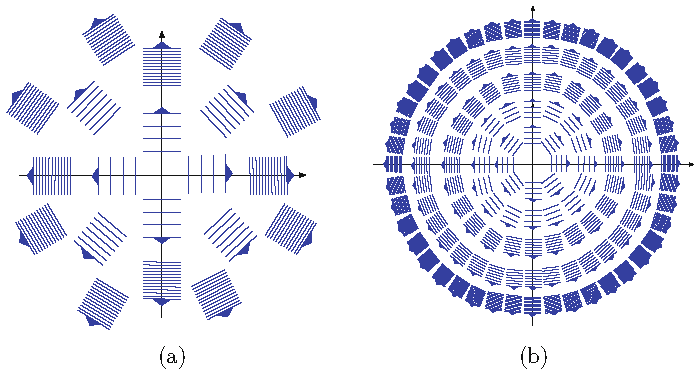
\includegraphics[width=0.830\linewidth]{images/vector/fig-5-32.pdf}
  \caption{流形 $\mathbb{R}^2$ 上的一形式 $xdx+ydy$，用两种不同的点阵表示为线桩网格. 箭头指向表示正方向. 注意右图中的线桩在中部开始看起来像是融合成同心圆（图像由 Vector Field Analyzer II, Version 2, Kawski, 2001 生成）}
  \label{fig:5-32}
\end{figure}

第二种方法做了类似的事情，但试图更进一步. 再次考虑图~\ref{fig:5-32}. 在第二幅图像中，点阵取得足够密，以至于特别是在中部，它们开始相互融合并形成同心圆. 在第二种方法中，阵点处的小图被相互连接起来，以在流形上提供一幅连续的图像. 当这确实可行时，这些图像是非常吸引人且容易思考的. 我们首先看看方法二在合适的时候是如何工作的，然后简要讨论方法二在一般情况下是如何失败的.

作为例子，图~\ref{fig:5-33} 在 $\mathbb{R}^2$ 上显示了一个一般的一形式 $\alpha$. 这里，阵点（未显示）处的线桩被尽可能好地连接起来，以生成覆盖流形的曲线. $\alpha(v)$ 的值（近似地）由向量 $v$ 刺穿的曲线条数给出. 流形 $\mathbb{R}^2$ 上二形式的情形被完全相同地处理，只是不是在每个阵点处画小的线桩，而是有小的方框补丁. 同样，有可能把这些方框连接起来，给出流形上二形式的粗略图像. 考虑图~\ref{fig:5-34}. 这里，流形 $\mathbb{R}^2$ 上的一个二形式被描绘在流形 $\mathbb{R}^2$ 上. 为了求出二形式 $\alpha$ 在任意给定点 $p$ 处的值，需要给出该点处的两个向量 $v_1$ 与 $v_2$. 那么 $\alpha_p(v_1,v_2)$ 的值由 $v_1$ 与 $v_2$ 张成的平行六面体内部的方框个数给出.

\begin{figure}[htbp]
  \centering
  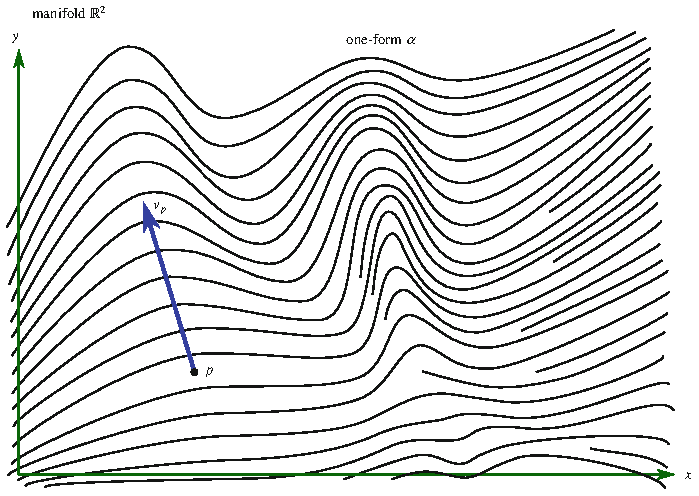
\includegraphics[width=0.876\linewidth]{images/vector/fig-5-33.pdf}
  \caption{流形 $\mathbb{R}^2$ 上展示了一个一形式 $\alpha$，所有"线桩"都被平滑地连接成曲线. 一形式作用在向量上的值（近似地）等于该向量"刺穿"的曲线的条数. 这里，$\alpha(v_p)\approx6$}
  \label{fig:5-33}
\end{figure}

在流形 $\mathbb{R}^3$ 上描绘一形式、二形式与三形式的尝试非常类似. 同样，选取一个点阵 $p_{ijk}=(x_i,y_j,z_k)$，并在每个这样的点处找到 $T_{p_{ijk}}\mathbb{R}^3$ 中该形式的图. 对在每个点 $p_{ijk}$ 处的一形式 $\alpha$，将有一桩二维薄片，类似于图~\ref{fig:5-17}. 然后，这些图中的每一幅的小副本将被叠加在每个阵点处的流形 $\mathbb{R}^3$ 上. 然后人们会尽可能好地尝试把这些薄片连接起来，得到一幅类似于图~\ref{fig:5-35} 的图. 薄片的紧密程度（换句话说，薄片彼此相隔多远）由特定的这个一形式决定. 为了求出 $\alpha(v)$ 的（近似）值，人们将数出向量 $v$ 刺穿的薄片张数. 所以，一形式 $10\alpha$ 的薄片彼此相距的距离是一形式 $\alpha$ 的薄片的十分之一.

\begin{figure}[htbp]
  \centering
  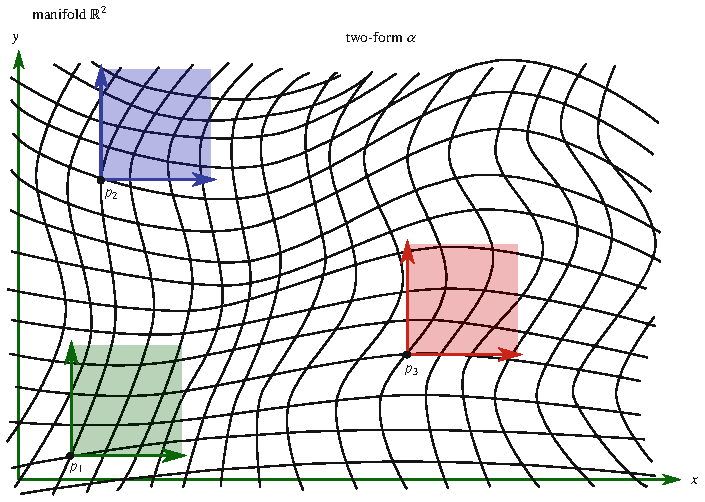
\includegraphics[width=0.875\linewidth]{images/vector/fig-5-34.pdf}
  \caption{流形 $\mathbb{R}^2$ 上展示了一个二形式 $\alpha$，所有方框都被平滑地连接起来. 单位向量 $e_1$ 与 $e_2$ 被描绘在点 $p_1$（绿）、$p_2$（蓝）与 $p_3$（红）处. 通过数出落在 $e_1$ 与 $e_2$ 在每个点处张成的平行六面体范围内的方框个数，可以（近似地）求出 $\alpha_{p_i}(e_1,e_2)$. 因此 $\alpha_{p_1}(e_1,e_2)\approx12$、$\alpha_{p_2}(e_1,e_2)\approx16$、$\alpha_{p_3}(e_1,e_2)\approx9$. 显然，虽然这是一幅漂亮的图，但它给出的答案只是非常近似的}
  \label{fig:5-34}
\end{figure}

对在每个点 $p_{ijk}$ 处的二形式 $\alpha$，将有一束"管子"，类似于图~\ref{fig:5-23}. 在每个阵点处，管子束的密度会变化，方向也会不同. 然后人们会尽可能好地尝试把这些薄片连接起来，得到一幅类似于图~\ref{fig:5-36} 的图，其中大小不同的管子蜿蜒穿过 $\mathbb{R}^3$. 管子排列的密度取决于二形式 $\alpha$ 的确切性质. 为了（近似地）求出 $\alpha(v_p,w_p)$，人们找到由 $v_p$ 与 $w_p$ 张成的平行六面体，并数出穿过这个平行六面体的管子根数.

\begin{figure}[htbp]
  \centering
  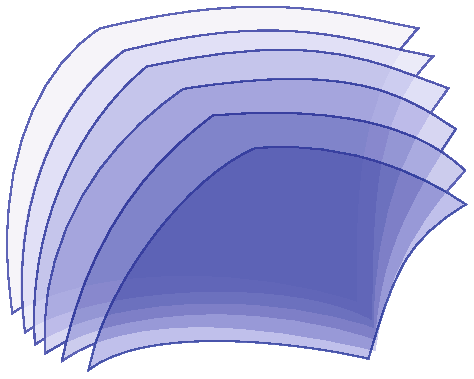
\includegraphics[width=0.656\linewidth]{images/vector/fig-5-35.pdf}
  \caption{$\mathbb{R}^3$ 中一个一般的一形式由填满 $\mathbb{R}^3$ 的薄片组成}
  \label{fig:5-35}
\end{figure}

对在每个点 $p_{ijk}$ 处的三形式 $\alpha$，将有一小组立方体，类似于图~\ref{fig:5-30}. 人们可以想象在每个阵点处有大小与方向各异的魔方. 然后这些立方体被尽可能好地全部连接起来，用小的立方体填满 $\mathbb{R}^3$. 我们在这里不再试图展示这一点. 求出 $\alpha(u_p,v_p,w_p)$ 的（近似）值归结为数出由 $u_p$、$v_p$、$w_p$ 张成的平行六面体内部的立方体个数.

\begin{figure}[htbp]
  \centering
  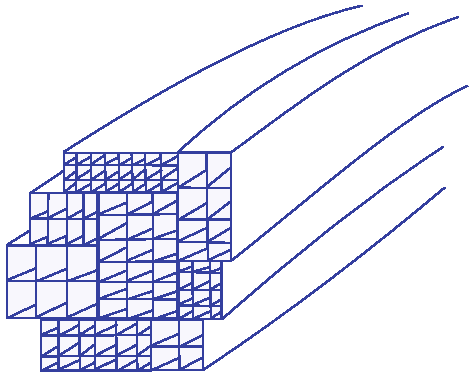
\includegraphics[width=0.657\linewidth]{images/vector/fig-5-36.pdf}
  \caption{$\mathbb{R}^3$ 中一个一般的二形式由填满 $\mathbb{R}^3$ 的管子组成}
  \label{fig:5-36}
\end{figure}

这种看待微分形式的方式有一些非常吸引人的地方，在某些情形下，它有助于提供一种在二维与三维流形上思考微分形式的额外方式. 不幸的是，在一般情况下方法二是失败的. 事实上，不用费多大力气就能找到方法二实际上无法可视化它们的形式的例子. 真正的问题之一是"连接"这件事. 从数学上看，这完全是障眼法，没有任何合理的理由. 事实上，一形式的每个线桩都位于不同的切空间中，所以"连接"线桩根本说不通. 而且，即使我们像上面那样在流形上画出这些图，也没有理由认为彼此靠近的阵点处的线桩会以允许它们被连接的方式定向，正如图~\ref{fig:5-32} 的情形那样. 对一般的一形式，它们不必如此. 当然，这也适用于三维流形的薄片桩与管子束.

一个必要但不充分的要求是，由微分形式的核给出的分布是可积的. 这将给出所谓的流形上的\newterm{foliation}{叶状结构}{foliation}，它允许线桩、薄片桩或管子束排列起来. 探索并解释这一点超出了本书的范围. 只需认识到，即使 $\mathbb{R}^3$ 上像 $xdy+dz$ 这样简单的一形式也无法使用方法二可视化.

然而，这种可视化微分形式的方式有时确实出现在物理学中. 物理学家并不太关心一种完全一般的可视化形式的方式，他们感兴趣的是对正在处理的物理问题与物理情形有效的可视化方式. 因此，这种方法在特定情形下确实有一些用处. 在合适的时候，它确实提供了一种非常好的思考形式的方式. 事实上，它为 Stokes 定理提供了一幅很好的配图，非常吸引人，将在第 11.6 节给出.

\section{Hodge 星算子可视化导引}

此时以数学上严谨的方式引入 Hodge 星算子有点棘手，因为许多必要的数学尚未引入，然而与本章相伴随的 Hodge 星算子的几何图确实相当漂亮且容易理解，所以现在是做这件事的自然时机. 因此我们将试图取得平衡，提供图背后的一些数学，但不足以让你被理论细节压垮. 眼下我们将限于三维的情形，并给出合理性论证而不是严谨的证明.

首先我们考虑下列向量空间
\begin{align*}
\bigwedge_p^0(\mathbb{R}^3)=\operatorname{span}\{1\}, \\
\bigwedge_p^1(\mathbb{R}^3)=\operatorname{span}\{dx,dy,dz\}=T_p^*\mathbb{R}^3, \\
\bigwedge_p^2(\mathbb{R}^3)=\operatorname{span}\{dx\wedge dy,dy\wedge dz,dz\wedge dx\}, \\
\bigwedge_p^3(\mathbb{R}^3)=\operatorname{span}\{dx\wedge dy\wedge dz\},
\end{align*}
它们的维数分别是一、三、三与一. 这些空间中的每一个都定义有所谓的\newterm{inner-product}{内积}{inner product}. 此时我们不去为一个严谨的定义而分心，只简单地说，本质上，向量空间上的内积把每一对向量与一个实数联系起来. 话虽如此，我们要做的是解释 $\bigwedge_p^1(\mathbb{R}^3)$ 与 $\bigwedge_p^2(\mathbb{R}^3)$ 上的内积，即我们最感兴趣的两个空间. 我们从空间 $\bigwedge_p^1(\mathbb{R}^3)$ 开始. $\bigwedge_p^1(\mathbb{R}^3)$ 上的内积由矩阵
\[
\begin{bmatrix}
1 & 0 & 0\\
0 & 1 & 0\\
0 & 0 & 1
\end{bmatrix}
\]
给出. 但这是如何工作的呢？假设我们有两个一形式元素 $\alpha,\beta\in\bigwedge_p^1(\mathbb{R}^3)$. 我们可以把这些元素按基元素写成余向量
\begin{align*}
\alpha=adx+bdy+cdz=[a,b,c], \\
\beta=rdx+sdy+tdz=[r,s,t].
\end{align*}
那么 $\alpha$ 与 $\beta$ 的内积，一般记为 $\langle\alpha,\beta\rangle$，由
\[
\langle\alpha,\beta\rangle=\langle[a,b,c],[r,s,t]\rangle
\equiv[a,b,c]
\begin{bmatrix}
1 & 0 & 0\\
0 & 1 & 0\\
0 & 0 & 1
\end{bmatrix}
[r,s,t]^T
\]
给出，即
\[
=[a,b,c]\begin{bmatrix}r\\s\\t\end{bmatrix}
=ar+bs+ct.
\]

我们花一点时间指出，用尖括号 $\langle\cdot,\cdot\rangle$ 表示内积是标准记号，它与我们前面用来表示微分形式与向量之间的典范配对 $\langle\cdot,\cdot\rangle$ 是完全不同的东西. 你必须仔细观察尖括号里面是什么，才能知道它们代表什么. 另外，注意我们隐含地假定基元素有一个顺序，$dx$ 第一，$dy$ 第二，$dz$ 第三. 只有知道了这个顺序，我们才知道如何写出表示内积的矩阵.

类似地，我们将用相同的矩阵
\[
\begin{bmatrix}
1 & 0 & 0\\
0 & 1 & 0\\
0 & 0 & 1
\end{bmatrix}
\]
定义 $\bigwedge_p^2(\mathbb{R}^3)$ 上的内积，它以完全相同的方式工作. 因此如果我们有
\begin{align*}
\eta=adx\wedge dy+bdy\wedge dz+cdz\wedge dx=[a,b,c], \\
\xi=rdx\wedge dy+sdy\wedge dz+tdz\wedge dx=[r,s,t],
\end{align*}
那么 $\eta$ 与 $\xi$ 的内积，记为 $\langle\eta,\xi\rangle$，由
\[
\langle\eta,\xi\rangle=\langle[a,b,c],[r,s,t]\rangle
\equiv[a,b,c]
\begin{bmatrix}
1 & 0 & 0\\
0 & 1 & 0\\
0 & 0 & 1
\end{bmatrix}
[r,s,t]^T
\]
给出，即
\[
=[a,b,c]\begin{bmatrix}r\\s\\t\end{bmatrix}
=ar+bs+ct.
\]
同样，我们隐含地假定基有一个顺序，这样我们才会知道如何写出矩阵.

现在我们有了真正定义 Hodge 星算子所必需的构件，它也被称为 Hodge 星对偶算子. Hodge 星算子是一个同构（或映射）$\ast:\bigwedge_p^k(\mathbb{R}^n)\to\bigwedge_p^{n-k}(\mathbb{R}^n)$，它把 $k$-形式送到 $(n-k)$-形式. 那么这个同构是如何定义的呢？对每个 $k$-形式 $\alpha$，存在唯一的一个 $(n-k)$-形式 $\ast\alpha$，使得对任意 $(n-k)$-形式 $\beta$ 都有
\begin{center}
\fbox{\parbox{0.88\textwidth}{\centering
Hodge 星算子：$\alpha\wedge\beta=\langle\ast\alpha,\beta\rangle\sigma$，对任意 $\beta$ 成立
}}
\end{center}
其中 $\langle\cdot,\cdot\rangle$ 表示 $\bigwedge_p^{n-k}(\mathbb{R}^n)$ 上的内积，$\sigma$ 是 $n$ 维体积形式. 所以，$\ast\alpha$ 是根据这个相当复杂的关系来定义的. 我们想把这一关系展开，看看它试图表达什么，
\[
\underbrace{\underbrace{\alpha}_{k\text{-形式}}\wedge\underbrace{\beta}_{(n-k)\text{-形式}}}_{\text{一个 }n\text{-形式}}
=
\langle\underbrace{\ast\alpha}_{(n-k)\text{-形式}},\underbrace{\beta}_{(n-k)\text{-形式}}\rangle
\underbrace{\sigma}_{\text{体积形式（一个 }n\text{-形式）}}.
\]

所以我们在等式的左边与右边各得到一个 $n$-形式. 回忆体积形式 $\sigma$ 是已知的，$\alpha$ 是给定的，而 $\beta$ 可以是任意 $(n-k)$-形式. 然后我们利用这个关系找出 $\ast\alpha$ 是哪一个 $(n-k)$-形式. 由于 $\beta$ 可以是任意 $(n-k)$-形式，这意味着无论选择哪一个 $(n-k)$-形式作为 $\beta$，我们总是找到完全相同的 $\ast\alpha$. 在某种意义上，这是相当惊人的. 但映射 $\ast$ 是唯一的，这一事实我们在这里不试图证明，所以无论选择哪一个 $(n-k)$-形式作为 $\beta$，都只有一个 $\ast\alpha$.

现在，让我们把这个关系真正用在我们三维的情形. 我们首先看映射 $\ast:\bigwedge_p^1(\mathbb{R}^3)\to\bigwedge_p^2(\mathbb{R}^3)$. 首先我们着手求 $\ast dx$. 由于我们知道 $\ast dx$ 是一个二形式，我们知道它必有形式
\[
\ast dx=a\,dx\wedge dy+b\,dy\wedge dz+c\,dz\wedge dx=[a,b,c]
\]
对某三个数 $a,b,c$. 我们的目标是用关系
\[
dx\wedge\beta=\langle\ast dx,\beta\rangle\,dx\wedge dy\wedge dz
\]
求出 $a$、$b$、$c$ 是什么. 眼下我们考虑由
\[
\beta=r\,dx\wedge dy+s\,dy\wedge dz+t\,dz\wedge dx=[r,s,t]
\]
给出的一般二形式 $\beta$. 所以我们的定义关系变成
\begin{align*}
& dx\wedge(r\,dx\wedge dy+s\,dy\wedge dz+t\,dz\wedge dx) \\
&=\langle\ast dx,r\,dx\wedge dy+s\,dy\wedge dz+t\,dz\wedge dx\rangle\,dx\wedge dy\wedge dz \\
&=\langle[a,b,c],[r,s,t]\rangle\,dx\wedge dy\wedge dz \\
&=(ar+bs+ct)\,dx\wedge dy\wedge dz.
\end{align*}
在左边我们有
\begin{align*}
dx\wedge(r\,dx\wedge dy+s\,dy\wedge dz+t\,dz\wedge dx)
=r\underbrace{dx\wedge dx\wedge dy}_{=0}+s\,dx\wedge dy\wedge dz+t\underbrace{dx\wedge dz\wedge dx}_{=0} \\
=s\,dx\wedge dy\wedge dz.
\end{align*}
合并起来我们有
\[
s\,dx\wedge dy\wedge dz=(ar+bs+ct)\,dx\wedge dy\wedge dz,
\]
这给出
\[
s=ar+bs+ct.
\]
由于我们的定义关系无论选择哪个 $\beta$ 都成立，如果我们选择满足 $r=1$、$s=0$、$t=0$ 的 $\beta$，这个等式会给出 $a=0$. 如果我们选择满足 $r=0$、$s=1$、$t=0$ 的 $\beta$，这个等式会给出 $b=1$. 如果我们选择满足 $r=0$、$s=0$、$t=1$ 的 $\beta$，这个等式会给出 $c=0$. 因此我们得到
\[
\ast dx=dy\wedge dz.
\]
$dx$ 与 $\ast dx$ 之间的关系在图~\ref{fig:5-37} 中以图形方式显示. $\ast dx=dy\wedge dz$ 的管子垂直于 $dx$ 的平面.

\begin{figure}[htbp]
  \centering
  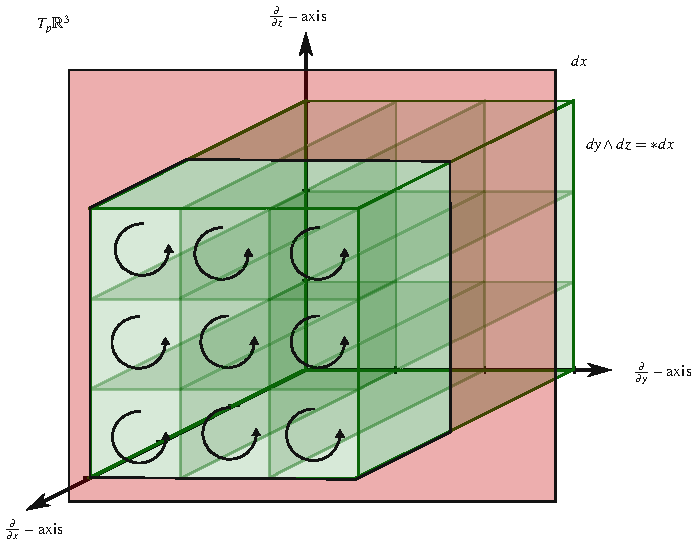
\includegraphics[width=0.828\linewidth]{images/vector/fig-5-37.pdf}
  \caption{$\ast dx$ 的管子垂直于 $dx$ 的平面. 即 $\ast dx=dy\wedge dz$}
  \label{fig:5-37}
\end{figure}

\begin{question}\label{q:5-23}
对下列 $\beta$ 证明 $dx\wedge\beta=\langle\ast dx,\beta\rangle\,dx\wedge dy\wedge dz$：
\begin{enumerate}
  \item[(a)] $\beta=7dx\wedge dy-3dy\wedge dz+2dz\wedge dx$，
  \item[(b)] $\beta=20dx\wedge dy+15dy\wedge dz-10dz\wedge dx$，
  \item[(c)] $\beta=-4dx\wedge dy-6dy\wedge dz-8dz\wedge dx$.
\end{enumerate}
\end{question}

我们将重做这个计算来求 $\ast dy$. 和以前一样，由于我们知道 $\ast dy$ 是一个二形式，我们知道它必有形式
\[
\ast dy=a\,dx\wedge dy+b\,dy\wedge dz+c\,dz\wedge dx=[a,b,c]
\]
对某三个数 $a,b,c$，并且我们希望用关系
\[
dy\wedge\beta=\langle\ast dy,\beta\rangle\,dx\wedge dy\wedge dz
\]
求出 $a$、$b$、$c$ 是什么. 同样，我们假设
\[
\beta=r\,dx\wedge dy+s\,dy\wedge dz+t\,dz\wedge dx=[r,s,t],
\]
结果得到
\begin{align*}
& dy\wedge(r\,dx\wedge dy+s\,dy\wedge dz+t\,dz\wedge dx) \\
&=\langle\ast dy,r\,dx\wedge dy+s\,dy\wedge dz+t\,dz\wedge dx\rangle\,dx\wedge dy\wedge dz \\
&=(ar+bs+ct)\,dx\wedge dy\wedge dz.
\end{align*}
左边变成
\begin{align*}
dy\wedge(r\,dx\wedge dy+s\,dy\wedge dz+t\,dz\wedge dx)
=r\underbrace{dy\wedge dx\wedge dy}_{=0}+s\underbrace{dy\wedge dy\wedge dz}_{=0}+t\,dy\wedge dz\wedge dx \\
=t\,dx\wedge dy\wedge dz.
\end{align*}
合并起来我们有
\[
t\,dx\wedge dy\wedge dz=(ar+bs+ct)\,dx\wedge dy\wedge dz,
\]
这给出
\[
t=ar+bs+ct.
\]
由于我们的定义关系无论选择哪个 $\beta$ 都成立，如果我们选择满足 $r=1$、$s=0$、$t=0$ 的 $\beta$，我们会得到 $a=0$. 如果我们选择满足 $r=0$、$s=1$、$t=0$ 的 $\beta$，我们会得到 $b=0$. 如果我们选择满足 $r=0$、$s=0$、$t=1$ 的 $\beta$，我们会得到 $c=1$. 因此我们会得到
\[
\ast dy=dz\wedge dx.
\]
再次注意，$\ast dy$ 的管子垂直于 $dy$ 的平面. 见图~\ref{fig:5-38}.

\begin{figure}[htbp]
  \centering
  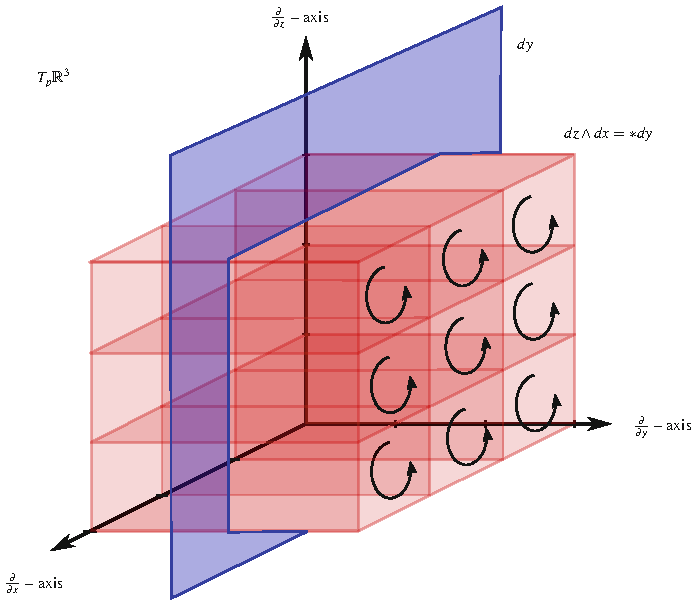
\includegraphics[width=0.830\linewidth]{images/vector/fig-5-38.pdf}
  \caption{$\ast dy$ 的管子垂直于 $dy$ 的平面. 即 $\ast dy=dz\wedge dx$}
  \label{fig:5-38}
\end{figure}

\begin{question}\label{q:5-24}
对下列 $\beta$ 证明 $dy\wedge\beta=\langle\ast dy,\beta\rangle\,dx\wedge dy\wedge dz$：
\begin{enumerate}
  \item[(a)] $\beta=7dx\wedge dy-3dy\wedge dz+2dz\wedge dx$，
  \item[(b)] $\beta=20dx\wedge dy+15dy\wedge dz-10dz\wedge dx$，
  \item[(c)] $\beta=-4dx\wedge dy-6dy\wedge dz-8dz\wedge dx$.
\end{enumerate}
\end{question}

\begin{question}\label{q:5-25}
利用定义恒等式 $dz\wedge\beta=\langle\ast dz,\beta\rangle\,dx\wedge dy\wedge dz$（对所有 $\beta\in\bigwedge_p^2(\mathbb{R}^3)$）求 $\ast dz$.
\end{question}

与 $\ast dz$ 相联系的图像显示 $\ast dz$ 的管子垂直于 $dz$ 的平面，见图~\ref{fig:5-39}.

\begin{figure}[htbp]
  \centering
  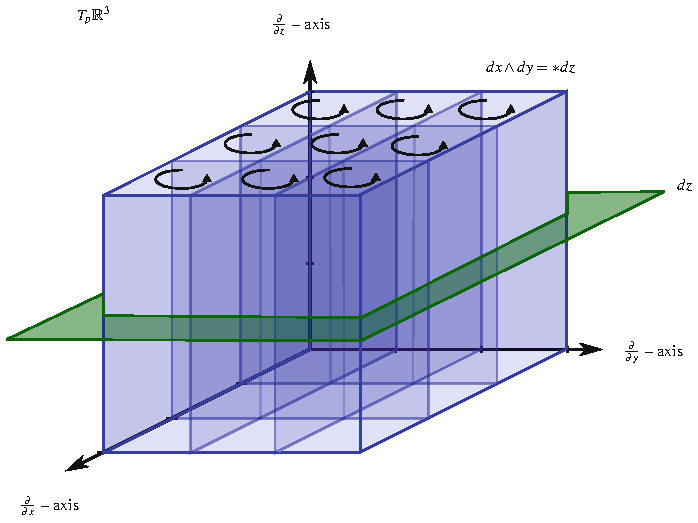
\includegraphics[width=0.827\linewidth]{images/vector/fig-5-39.pdf}
  \caption{$\ast dz$ 的管子垂直于 $dz$ 的平面. 即 $\ast dz=dx\wedge dy$}
  \label{fig:5-39}
\end{figure}

\begin{question}\label{q:5-26}
对下列 $\beta$ 证明 $dz\wedge\beta=\langle\ast dz,\beta\rangle\,dx\wedge dy\wedge dz$：
\begin{enumerate}
  \item[(a)] $\beta=7dx\wedge dy-3dy\wedge dz+2dz\wedge dx$，
  \item[(b)] $\beta=20dx\wedge dy+15dy\wedge dz-10dz\wedge dx$，
  \item[(c)] $\beta=-4dx\wedge dy-6dy\wedge dz-8dz\wedge dx$.
\end{enumerate}
\end{question}

\begin{question}\label{q:5-27}
利用 Hodge 星算子的定义求 $*(dx\wedge dy)$、$*(dy\wedge dz)$ 与 $*(dz\wedge dx)$.
\end{question}

\begin{question}\label{q:5-28}
你有时会看到 Hodge 星算子的另一种定义. 由于这是一个处理起来稍微容易的定义，我们把它留作练习. 证明 Hodge 星算子的这个替代定义
\[
\alpha\wedge\ast\beta=\langle\alpha,\beta\rangle\sigma,\qquad\text{对任意 }\alpha
\]
对 $*dx$、$*dy$、$*dz$、$*(dx\wedge dy)$、$*(dy\wedge dz)$、$*(dz\wedge dx)$ 给出相同的值.
\end{question}

现在我们来看 $\mathbb{R}^4$ 上形式的 Hodge 星对偶算子. 在四维中，试图画图要困难得多，但数学计算是相当直接的. 首先我们定义记号与我们的空间. 我们将用 $x_1,x_2,x_3,x_4$ 作为我们的笛卡尔坐标函数. 在 $\mathbb{R}^3$ 中循环书写以保持整洁很管用，但在 $\mathbb{R}^4$ 中就没有那么有用了，所以我们不再这样做. 这里的约定是使用递增顺序. 我们将使用的空间是
\begin{align*}
\bigwedge^0(\mathbb{R}^4)=C(\mathbb{R}^4)=\mathbb{R}^4\text{ 上的函数}, \\
\bigwedge^1(\mathbb{R}^4)=\operatorname{Span}\{dx_1,dx_2,dx_3,dx_4\}, \\
\bigwedge^2(\mathbb{R}^4)=\operatorname{Span}\{dx_1\wedge dx_2,dx_1\wedge dx_3,dx_1\wedge dx_4,dx_2\wedge dx_3,dx_2\wedge dx_4,dx_3\wedge dx_4\}, \\
\bigwedge^3(\mathbb{R}^4)=\operatorname{Span}\{dx_1\wedge dx_2\wedge dx_3,dx_1\wedge dx_2\wedge dx_4,dx_1\wedge dx_3\wedge dx_4,dx_2\wedge dx_3\wedge dx_4\}, \\
\bigwedge^4(\mathbb{R}^4)=\operatorname{Span}\{dx_1\wedge dx_2\wedge dx_3\wedge dx_4\}.
\end{align*}
这些空间上的内积（Hodge 星对偶定义右边所必需的）由单位矩阵给出. 目前我们对此不作过多追究，但流形的度量（内积正是由它导出的）我们将在第 A.6 节更详细地讨论.

现在我们利用问题~\ref{q:5-28} 中给出的 Hodge 星对偶的定义求一个一形式基元素的 Hodge 星对偶，
\begin{align*}
dx_1\wedge\ast dx_1=\underbrace{\langle dx_1,dx_1\rangle}_{=1}\,dx_1\wedge dx_2\wedge dx_3\wedge dx_4 \\
\Longrightarrow\ \ast dx_1=dx_2\wedge dx_3\wedge dx_4.
\end{align*}
注意，通过把 $dx_1$ 与 $\ast dx_1$ 楔起来，我们得以在等式右边利用 $\bigwedge^1(\mathbb{R}^4)$ 上内积的优良性质，在那里我们有 $\langle dx_1,dx_1\rangle=1$. 求二形式基元素的 Hodge 星对偶类似：
\begin{align*}
(dx_1\wedge dx_2)\wedge\ast(dx_1\wedge dx_2)=\underbrace{\langle dx_1\wedge dx_2,dx_1\wedge dx_2\rangle}_{=1}\,dx_1\wedge dx_2\wedge dx_3\wedge dx_4 \\
\Longrightarrow\ \ast(dx_1\wedge dx_2)=dx_3\wedge dx_4.
\end{align*}

\begin{question}\label{q:5-29}
求 $\ast dx_2$、$\ast dx_3$、$\ast dx_4$.
\end{question}

\begin{question}\label{q:5-30}
求 $*(dx_1\wedge dx_3)$、$*(dx_1\wedge dx_4)$、$*(dx_2\wedge dx_3)$、$*(dx_2\wedge dx_4)$、$*(dx_3\wedge dx_4)$.
\end{question}

\begin{question}\label{q:5-31}
求 $*(dx_1\wedge dx_2\wedge dx_3)$、$*(dx_1\wedge dx_2\wedge dx_4)$、$*(dx_1\wedge dx_3\wedge dx_4)$、$*(dx_2\wedge dx_3\wedge dx_4)$.
\end{question}

\begin{question}\label{q:5-32}
求 $*(dx_1\wedge dx_2\wedge dx_3\wedge dx_4)$.
\end{question}

\section{小结、参考文献与问题}

\subsection{小结}

我们现在花一点时间用一些评论来结束本章. 如果你是数学专业的学生，你可能永远不会在你的任何教科书里看到这种描绘或表示微分形式的方式；我肯定从来没有. 然而，如果你是物理专业的学生，那么很有可能会看到以这种方式讨论或呈现微分形式，无论是在电磁学课程中，还是在相对论课程中. 这些图像在试图理解某些方程并描绘这些方程背后的物理现象时非常有用. 我们将在后续章节详细探讨其中的一些物理应用. 尽管这些图在描绘方程试图表达的意思方面能提供很大的帮助，但在实际计算中使用它们通常是困难的，而且不值得费力，因为它们只给出近似答案. 使用微分形式的计算规则来计算精确的数值答案，并使用这些图来辅助概念性的理解.

此外，人们可以发展这些图像的高维类似物. 例如，把时间考虑进去，从相对论之前的欧几里得视角来看待时空，就会得到它的一个四维版本. 在狭义相对论与广义相对论两种情形下把时间包括进来也会得到四维版本，但在这些情形下，由于流形上的度量（想想内积）不同，基于内积的 Hodge 星算子也会改变. 然而，维度越高，使用这些图就越困难，使用得也越少，尽管想象 1 维与 $n-1$ 维的情形通常仍然是够清楚的.

Hodge 星算子的两个等价定义如下给出，
\begin{center}
\fbox{\parbox{0.88\textwidth}{\centering
Hodge 星算子定义一：$\alpha\wedge\beta=\langle\ast\alpha,\beta\rangle\sigma$，对任意 $\beta$ 成立；\\
Hodge 星算子定义二：$\alpha\wedge\ast\beta=\langle\alpha,\beta\rangle\sigma$，对任意 $\alpha$ 成立
}}
\end{center}

\subsection{参考文献与进一步阅读}

本章的材料几乎只出现在物理学中. 这是有原因的——作为一种思考微分形式的严谨方式，它在几个方面有所欠缺. 关于这种在流形上可视化形式的方式及其欠缺之处的批评，见 Bachman~\cite{ref04}. 但作为一种在各类物理情形中相当宽松地思考微分形式的方式，它相当有用，并且从物理系统的角度来看可能相当富有启发性. 正如本章开头提到的，这部分材料的主要来源是 Misner、Thorne 和 Wheeler~\cite{ref34}，不过也使用了 Dray~\cite{ref16}、Warnick、Selfridge 和 Arnold~\cite{ref49}、Warnick 与 Russer~\cite{ref48} 以及 DesChamps~\cite{ref13}. 所有这些来源都属于物理学的领域. 事实上，最后三篇文献强烈主张把这些可视化微分形式的技术作为教授电磁学的教学工具，尽管我们不知道有任何相当完整的实际尝试. 唯一另一个试图沿着本章材料思路给出几何解释的真正数学来源是 Burke~\cite{ref08}，而他的目标读者同样是在职物理学家. 用于生成 $\mathbb{R}^2$ 中一形式的线桩图像的软件是 Kawski~\cite{ref28} 编写的 Vector Field Analyzer II，可在网上获得.

\subsection{问题}

\begin{question}\label{q:5-33}
画出 $\mathbb{R}^2$ 上的坐标函数 $z$，并求出坐标函数 $y$ 沿下列向量的"rise"：
\begin{enumerate}
  \item[(a)] $\binom{0}{1}$，即从点 $(0,0)$ 到点 $(0,1)$，
  \item[(b)] $\binom{1}{1}$，即从点 $(0,0)$ 到点 $(1,1)$，
  \item[(c)] $\binom{-1}{2}$，即从点 $(0,0)$ 到点 $(-1,2)$，
  \item[(d)] $\binom{2}{-3}$，即从点 $(0,0)$ 到点 $(2,-3)$.
\end{enumerate}
\end{question}

\begin{question}\label{q:5-34}
画出表示 $\mathbb{R}^2$ 上下列一形式的图：$7dx$、$-3dy$、$-\frac23dx$、$-\frac13dy$ 与 $\frac25dy$.
\end{question}

\begin{question}\label{q:5-35}
画出 $\mathbb{R}^2$ 上下列一形式的图形表示：$\frac12dx+2dy$、$-\frac13dx-\frac12dy$ 与 $-dx-\frac23dy$.
\end{question}

\begin{question}\label{q:5-36}
为下列每个二形式在 $\mathbb{R}^2$ 上画出三种图形表示：$5dx\wedge dy$、$\frac12dx-\frac12dy$ 与 $2dx+\frac23dy$.
\end{question}

\begin{question}\label{q:5-37}
在 $\mathbb{R}^3$ 上画出一形式 $dx-dy$、$-dx+dy$、$dy-dz$ 与 $-dx-dz$ 的草图.
\end{question}

\begin{question}\label{q:5-38}
为下列每个二形式在 $\mathbb{R}^3$ 上找出两种图形表示：$5dx\wedge dy$、$6dy\wedge dz$ 与 $\frac14dz\wedge dx$.
\end{question}

\begin{question}\label{q:5-39}
为下列每个二形式在 $\mathbb{R}^3$ 上画出一幅草图：$3dy\wedge dz+2dz\wedge dx$、$dx\wedge dy+3dz\wedge dx$ 与 $2dx\wedge dy+4dy\wedge dz+3dz\wedge dx$.
\end{question}

\begin{question}\label{q:5-40}
在 $\mathbb{R}^3$ 上画出二形式 $-dx\wedge dy+dy\wedge dz$、$dx\wedge dy-dy\wedge dz$ 与 $-dx\wedge dy-dy\wedge dz$ 的草图. 负号有什么影响？用一些精心选择的向量来帮助你弄清楚.
\end{question}

\begin{question}\label{q:5-41}
把下面的一形式与图~\ref{fig:5-40} 中描绘的图像配对：
\begin{enumerate}
  \item[(a)] $\sin(x)dx+ydy$，
  \item[(b)] $dx-dy$，
  \item[(c)] $xdx+\cos(y)dy$，
  \item[(d)] $\sin(x)dx+xdy$.
\end{enumerate}
\end{question}

\begin{figure}[htbp]
  \centering
  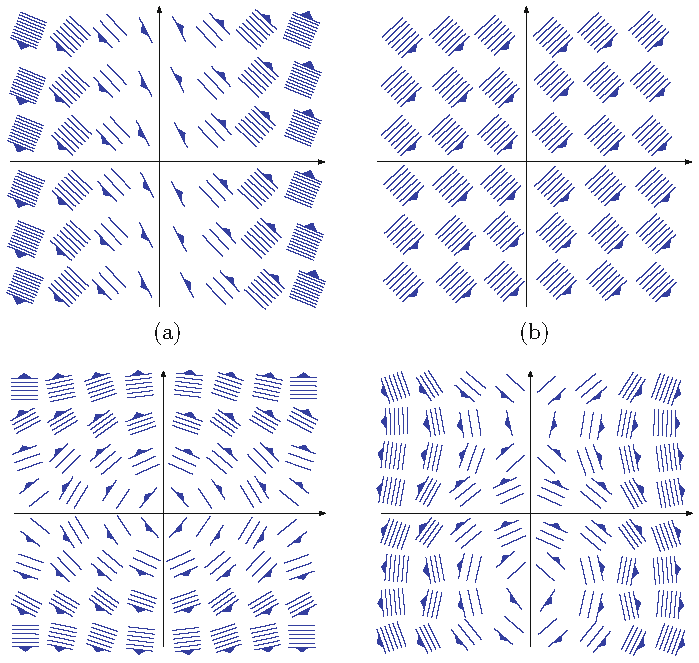
\includegraphics[width=0.829\linewidth]{images/vector/fig-5-40.pdf}
  \caption{问题~\ref{q:5-41} 的图像（图像由 Vector Field Analyzer II, Version 2, Kawski, 2001 生成）.}
  \label{fig:5-40}
\end{figure}

\begin{question}\label{q:5-42}
设流形是 $\mathbb{R}^4$. 求 $\ast dx_2$、$\ast dx_3$、$\ast dx_4$.
\end{question}

\begin{question}\label{q:5-43}
设流形是 $\mathbb{R}^4$. 求 $*(dx_1\wedge dx_3)$、$*(dx_1\wedge dx_4)$、$*(dx_2\wedge dx_3)$、$*(dx_2\wedge dx_4)$、$*(dx_3\wedge dx_4)$.
\end{question}

\begin{question}\label{q:5-44}
设流形是 $\mathbb{R}^4$. 求 $*(dx_1\wedge dx_2\wedge dx_3)$、$*(dx_1\wedge dx_2\wedge dx_4)$、$*(dx_1\wedge dx_3\wedge dx_4)$、$*(dx_2\wedge dx_3\wedge dx_4)$.
\end{question}

\begin{question}\label{q:5-45}
设流形是 $\mathbb{R}^4$. 求 $*(dx_1\wedge dx_2\wedge dx_3\wedge dx_4)$.
\end{question}

% 第 6 章 前推与拉回
\chapter{前推与拉回}

本章我们引入两个极其重要的概念：向量的\newterm{push-forward}{前推}{push-forward}与微分形式的\newterm{pull-back}{拉回}{pull-back}. 在第 1 节我们仔细考察一个简单的\newterm{coordinate-transformation}{坐标变换}{coordinate transformation}，看看这个坐标变换对单位正方形的体积有什么影响. 这使我们在第 2 节能够引出向量的前推. 向量的前推使我们能够把向量从一个流形移动，或者说"前推"，到另一个流形. 在坐标变换的情形下，两个流形实际上是同一个流形，只是配备了不同的坐标系.

利用微分形式吃进向量这一事实，我们在第 3 节用向量的前推来定义微分形式的拉回，其中我们把一个流形上的微分形式"拉回"到另一个流形. 同样，在坐标变换的情形下，两个流形实际上真的是同一个流形，只是配备了不同的坐标系. 然后我们更仔细地考察\newterm{volume-form}{体积形式}{volume form}的拉回，它在第 3 节的积分问题中起着至关重要的作用. 我们能够为体积形式的拉回导出一个漂亮的公式，其中包含坐标变换的 Jacobian 矩阵.

然后我们利用前推与拉回仔细考察一些熟悉的例子. 极坐标在第 4 节讨论，柱坐标与球坐标在第 5 节讨论. 第 6 节我们考虑非体积形式的微分形式的拉回，最后在第 7 节我们证明三个恒等式，它们对我们做涉及拉回的计算至关重要.

\section{坐标变换：线性例子}

本节是我们对坐标变换的初次考察. 我们不打算在本节做到完全严谨，这实际上只是想让我们对大局看得更清楚一些. 在我们开始摆弄漂亮的极坐标和球坐标之前，让我们考虑一个简单的情形. 坐标变换无非是 $\mathbb{R}^n$ 与 $\mathbb{R}^n$ 之间既是单射又是满射的映射. 由于 $\mathbb{R}^n$ 与 $\mathbb{R}^n$ 相同，我们常常把它想成 $\mathbb{R}^n$ 到自身的映射. 考虑由
\[
u(x,y)=x+y,\qquad v(x,y)=x-y
\]
给出的两个映射 $u,v:\mathbb{R}^2\to\mathbb{R}^2$.

图~\ref{fig:6-1} 显示了这个坐标变换. 左边是用 $xy$ 坐标表示的 $\mathbb{R}^2$，我们也把它称为 $xy$ 平面或 $\mathbb{R}^2_{xy}$；右边是用 $uv$ 坐标表示的 $\mathbb{R}^2$，我们也把它称为 $uv$ 平面或 $\mathbb{R}^2_{uv}$. 所以，即使 $\mathbb{R}^2$ 就是 $\mathbb{R}^2$，我们也根据所用的坐标对这两个副本作出区分. 在左上角，来自 $xy$ 平面的 $x$ 网格线与 $y$ 网格线被映射到右边 $uv$ 平面上的直线；在右下角，$u$ 网格线与 $v$ 网格线被映射到左边 $xy$ 平面上的直线.

\begin{figure}[htbp]
  \centering
  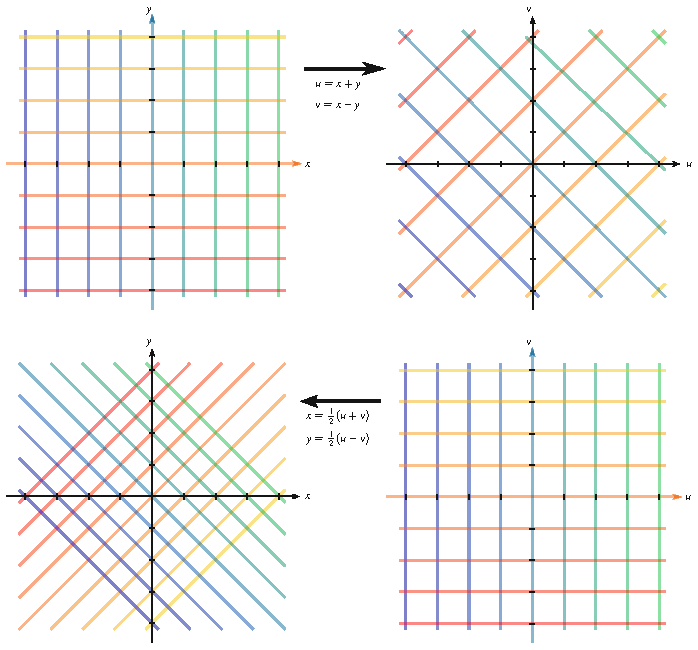
\includegraphics[width=0.960\linewidth]{images/vector/fig-6-1.pdf}
  \caption{平面 $\mathbb{R}^2_{xy}$（左）与 $\mathbb{R}^2_{uv}$（右）. 由 $u(x,y)=x+y$ 与 $v(x,y)=x-y$ 给出的坐标变换位于顶部（从左到右）. 逆坐标变换 $x(u,v)=\frac12(u+v)$ 与 $y(u,v)=\frac12(u-v)$ 位于底部（从右到左）. 颜色编码显示了各条直线是如何映射的}
  \label{fig:6-1}
\end{figure}

\begin{question}\label{q:6-1}
求下列直线在映射 $u=x+y$ 与 $v=x-y$ 下的像，并把你求出的结果与图~\ref{fig:6-1} 顶部所示的映射进行比较.
\begin{enumerate}
  \item[(a)] $x=0$
  \item[(b)] $x=1$
  \item[(c)] $x=4$
  \item[(d)] $y=0$
  \item[(e)] $y=1$
  \item[(f)] $y=-3$
\end{enumerate}
\end{question}

\begin{question}\label{q:6-2}
求下列直线在逆映射 $x=\frac12(u+v)$ 与 $y=\frac12(u-v)$ 下的像，并把你求出的结果与图~\ref{fig:6-1} 底部所示的映射进行比较.
\begin{enumerate}
  \item[(a)] $u=0$
  \item[(b)] $u=1$
  \item[(c)] $u=4$
  \item[(d)] $v=0$
  \item[(e)] $v=1$
  \item[(f)] $v=-3$
\end{enumerate}
\end{question}

我们用坐标函数 $u=x+y$ 与 $v=x-y$ 把平面 $\mathbb{R}^2_{xy}$ 中的点映射为 $\mathbb{R}^2_{uv}$ 中的点，如下所示：
\[
\begin{array}{lcl}
(x,y)&\longrightarrow&(x+y,x-y)=(u,v)\\
(0,0)&\longrightarrow&(0+0,0-0)=(0,0)\\
(1,0)&\longrightarrow&(1+0,1-0)=(1,1)\\
(1,1)&\longrightarrow&(1+1,1-1)=(2,0)\\
(0,1)&\longrightarrow&(0+1,0-1)=(1,-1).
\end{array}
\]
当我们在 $\mathbb{R}^2_{xy}$ 中绕着单位正方形移动时，可以跟踪 $\mathbb{R}^2_{uv}$ 中发生的情况：
\[
\begin{array}{ll}
(x,y):&(0,0)\longrightarrow(1,0)\longrightarrow(1,1)\longrightarrow(0,1)\longrightarrow(0,0)\\
(u,v):&(0,0)\longrightarrow(1,1)\longrightarrow(2,0)\longrightarrow(1,-1)\longrightarrow(0,0).
\end{array}
\]

由此我们可以看到，如图~\ref{fig:6-2} 所示，来自 $xy$ 坐标的单位正方形被映射为 $uv$ 坐标中的菱形. 注意，当你沿着图~\ref{fig:6-2} 左边所示的 $xy$ 坐标中的单位正方形以逆时针方向移动时，你是在沿着图~\ref{fig:6-2} 右边所示的 $uv$ 坐标中的菱形以顺时针方向移动. 还有另一个有趣的差别. 考虑 $xy$ 平面中单位正方形的面积，它的面积是 $1$；而 $uv$ 平面中菱形的面积，即单位正方形的像，其面积是 $2$.

\begin{figure}[htbp]
  \centering
  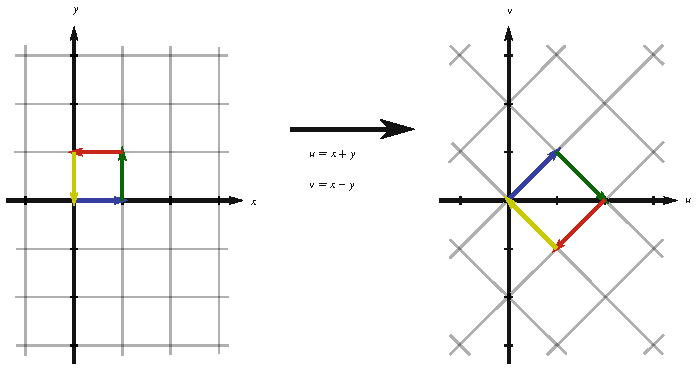
\includegraphics[width=0.960\linewidth]{images/vector/fig-6-2.pdf}
  \caption{$\mathbb{R}^2_{xy}$ 中的单位正方形（左）被映射为 $\mathbb{R}^2_{uv}$ 中的菱形（右）. 注意定向从逆时针变为顺时针，面积从 1 增加到 2}
  \label{fig:6-2}
\end{figure}

\begin{figure}[htbp]
  \centering
  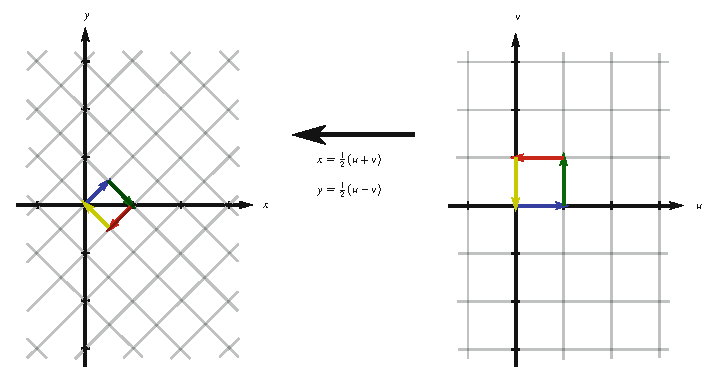
\includegraphics[width=0.960\linewidth]{images/vector/fig-6-3.pdf}
  \caption{$\mathbb{R}^2_{uv}$ 中的单位正方形（右）被映射为 $\mathbb{R}^2_{xy}$ 中的菱形（左）. 注意定向从逆时针变为顺时针，面积从 1 减小到二分之一}
  \label{fig:6-3}
\end{figure}

\begin{question}\label{q:6-3}
证明在逆映射 $x=\frac12(u+v)$ 与 $y=\frac12(u-v)$ 下点 $(0,0)$、$(1,0)$、$(1,1)$ 和 $(0,1)$ 会怎样.
\end{question}

类似地，如果我们用逆映射把来自 $uv$ 坐标平面（如图~\ref{fig:6-3} 右边所示）的单位正方形送到 $xy$ 坐标平面，那么我们在 $xy$ 坐标平面中得到一个菱形（如图~\ref{fig:6-3} 左边所示），其面积为原来的一半且方向反转. 接下来注意到
\[
dx\wedge dy\underbrace{\left(\binom{1}{0}_{xy(0,0)},\binom{0}{1}_{xy(0,0)}\right)}_{\text{xy 平面中的向量}}=\left|\begin{matrix}1&0\\0&1\end{matrix}\right|=1,
\]
以及
\[
du\wedge dv\underbrace{\left(\binom{1}{0}_{uv(0,0)},\binom{0}{1}_{uv(0,0)}\right)}_{\text{uv 平面中的向量}}=\left|\begin{matrix}1&0\\0&1\end{matrix}\right|=1,
\]
所以 $dx\wedge dy$ 是 $xy$ 平面的\newterm{area-form}{面积形式}{area form}，而 $du\wedge dv$ 是 $uv$ 平面的面积形式.

首先我们把 $du\wedge dv$ 写成 $dx\wedge dy$ 的形式. 其中一部分已经完成了. 由于 $u=x+y$ 与 $v=x-y$，我们有
\[
du=d(x+y)=dx+dy,\qquad dv=d(x-y)=dx-dy
\]
所以我们有
\begin{align*}
du\wedge dv&=(dx+dy)\wedge(dx-dy)\\
&=dx\wedge(dx-dy)+dy\wedge(dx-dy)\\
&=dx\wedge dx-dx\wedge dy+dy\wedge dx-dy\wedge dy\\
&=-dx\wedge dy-dx\wedge dy\\
&=-2dx\wedge dy.
\end{align*}

接下来我们把 $dx\wedge dy$ 写成 $du\wedge dv$ 的形式. 在上面的问题~\ref{q:6-3}中你证明了，用 $u$ 和 $v$ 解出 $x$ 和 $y$ 得到
\[
x=\frac12(u+v),\qquad y=\frac12(u-v)
\]
这反过来又给出
\[
dx=d\left(\frac12(u+v)\right)=\frac12du+\frac12dv,\qquad
dy=d\left(\frac12(u-v)\right)=\frac12du-\frac12dv
\]
所以我们有
\begin{align*}
dx\wedge dy&=\left(\frac12du+\frac12dv\right)\wedge\left(\frac12du-\frac12dv\right)\\
&=\frac14dv\wedge du-\frac14du\wedge dv\\
&=-\frac12du\wedge dv.
\end{align*}
总而言之，我们刚才所做的就是计算 $xy$ 面积形式与 $uv$ 面积形式之间的下列关系
\[
du\wedge dv=-2dx\wedge dy,\qquad dx\wedge dy=-\frac12du\wedge dv.
\]

把图~\ref{fig:6-2} 与图~\ref{fig:6-3} 中发生的事情与面积形式之间的关系进行比较. 它们彼此之间有什么关系？首先，我们尝试理解体积形式的关系告诉我们什么. 首先考虑图~\ref{fig:6-2}，其中 $xy$ 平面中的单位正方形被映射为 $uv$ 平面中的菱形. $uv$ 平面中菱形的体积是 $xy$ 平面中单位正方形体积的 $-2$ 倍. 我们可以看出 2 从何而来：注意到 $xy$ 平面中的单位正方形被映射为面积是其两倍的 $uv$ 平面中的菱形. 那么负号又从何而来？来自注意到 $xy$ 平面中的逆时针旋转变成了 $uv$ 平面中的顺时针旋转. 这就是我们的有向体积. 所以，我们所展示的必然与恒等式
\[
du\wedge dv=-2dx\wedge dy
\]
有某种关系.

接下来考虑图~\ref{fig:6-3}，其中 $uv$ 平面中的单位正方形被映射为 $xy$ 平面中的菱形. $xy$ 平面中菱形的面积是 $uv$ 平面中单位正方形体积的 $-\frac12$ 倍. 这意味着 $uv$ 平面中（有向）体积为 1 的单位正方形被映射为 $xy$ 平面中（有向）体积为 $-\frac12$ 的菱形，其中负号再次表明，绕着 $uv$ 平面中正方形的逆时针旋转变成了绕着 $xy$ 平面中菱形的顺时针旋转. 同样，这显然与恒等式
\[
dx\wedge dy=-\frac12du\wedge dv
\]
有某种关系.

回想一下，当我们在第 1.2 节推导行列式的公式时，我们一开始规定了我们认为体积应当具有的三个基本而直观的性质：
\begin{enumerate}
  \item 单位立方体的体积应为 1（在任何维数下）.
  \item 退化的平行六面体（即 $\mathbb{R}^n$ 中小于 $n$ 维的平行六面体）的 $n$ 维体积应为零.
  \item 把一条边缩放 $c$ 倍，体积应改变 $c$ 倍.
\end{enumerate}
通过假设我们的体积函数 $D$ 只具有这三个性质，我们发现了第四个性质：交换（对调）平行六面体的两条边也会改变体积的符号. 换句话说，在我们对体积的直观认识中，最基本的是\newterm{orientation}{定向}{orientation}的概念. 在三维中，定向常常被伪装成"右手法则". 见图~\ref{fig:6-4}.

\begin{figure}[htbp]
  \centering
  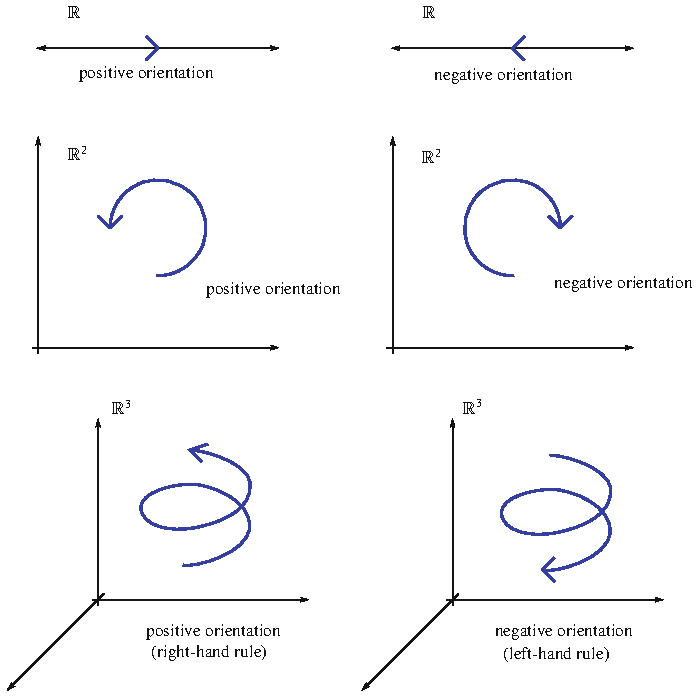
\includegraphics[width=0.829\linewidth]{images/vector/fig-6-4.pdf}
  \caption{$\mathbb{R}$（顶部）、$\mathbb{R}^2$（中部）与 $\mathbb{R}^3$（底部）的两种定向}
  \label{fig:6-4}
\end{figure}

在过去的几页中我们一直有点不严谨，但至少现在你可能开始看到，不同坐标系中的这些体积形式是如何相互关联的——当你从一个坐标系移动到另一个坐标系时，它们以某种方式编码了体积的变化. 这正是我们在积分时换元时会用到的那类东西.

现在我们想更仔细地考察体积形式. $xy$ 平面中的单位正方形由 $xy$ 平面中的向量
\[
\binom{1}{0}_{xy(0,0)},\qquad\binom{0}{1}_{xy(0,0)}
\]
给出（张成）. 换句话说，由这两个向量张成的平行六面体就是单位正方形. 这里我们在下标中用 $xy$ 表示这些向量所在的坐标平面. 这些向量在坐标变换 $u=x+y$ 与 $v=x-y$ 下的投影由
\[
\binom{1}{0}_{xy(0,0)}\longmapsto\binom{1}{1}_{uv(0,0)},\qquad
\binom{0}{1}_{xy(0,0)}\longmapsto\binom{1}{-1}_{uv(0,0)}
\]
给出. 见图~\ref{fig:6-5}. 容易计算出
\begin{align*}
dx\wedge dy\left(\binom{1}{0}_{xy(0,0)},\binom{0}{1}_{xy(0,0)}\right)=\left|\begin{matrix}1&0\\0&1\end{matrix}\right|=1, \\
du\wedge dv\left(\binom{1}{1}_{uv(0,0)},\binom{1}{-1}_{uv(0,0)}\right)=\left|\begin{matrix}1&1\\1&-1\end{matrix}\right|=-2.
\end{align*}

\begin{figure}[htbp]
  \centering
  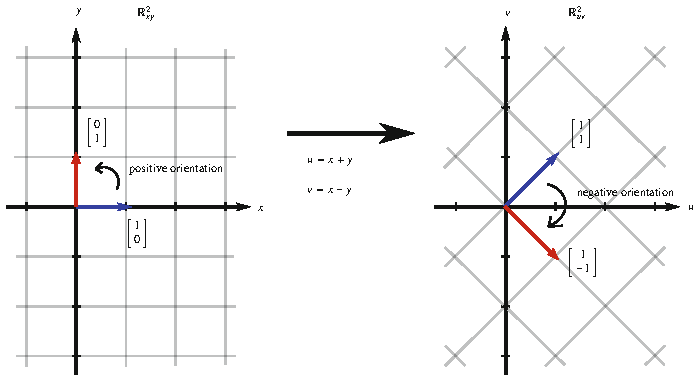
\includegraphics[width=0.960\linewidth]{images/vector/fig-6-5.pdf}
  \caption{$xy$ 平面中的基向量被映射为 $uv$ 平面中的两个向量. 注意定向发生变化}
  \label{fig:6-5}
\end{figure}

回想面积形式会求输入向量张成的平行六面体的面积，这与我们从图中预期的完全一致. 我们也开始对恒等式
\[
dx\wedge dy=-\frac12du\wedge dv
\]
的含义有了更清晰的图景. 实际上我们有
\[
dx\wedge dy\left(\binom{1}{0}_{xy(0,0)},\binom{0}{1}_{xy(0,0)}\right)
=-\frac12du\wedge dv\left(\binom{1}{1}_{uv(0,0)},\binom{1}{-1}_{uv(0,0)}\right).
\]
面积形式 $dx\wedge dy$ 必须吃进来自 $xy$ 平面的向量，而面积形式 $du\wedge dv$ 必须吃进来自 $uv$ 平面的向量. 此外，面积形式 $du\wedge dv$ 所吃进的向量，正是面积形式 $dx\wedge dy$ 所吃进的向量在映射 $u$ 与 $v$（$u=x+y$ 与 $v=x-y$）下的投影.

类似地，$uv$ 平面中的单位正方形由向量
\[
\binom{1}{0}_{uv(0,0)},\qquad\binom{0}{1}_{uv(0,0)}
\]
张成. 在上述坐标变换的逆变换 $x=\frac12(u+v)$ 与 $y=\frac12(u-v)$ 下，这些向量的投影由
\[
\binom{1}{0}_{uv(0,0)}\longmapsto\binom{1/2}{1/2}_{xy(0,0)},\qquad
\binom{0}{1}_{uv(0,0)}\longmapsto\binom{1/2}{-1/2}_{xy(0,0)}
\]
给出. 见图~\ref{fig:6-6}. 同样，容易计算出
\begin{align*}
du\wedge dv\left(\binom{1}{0}_{uv(0,0)},\binom{0}{1}_{uv(0,0)}\right)=\left|\begin{matrix}1&0\\0&1\end{matrix}\right|=1, \\
dx\wedge dy\left(\binom{1/2}{1/2}_{xy(0,0)},\binom{1/2}{-1/2}_{xy(0,0)}\right)=\left|\begin{matrix}1/2&1/2\\1/2&-1/2\end{matrix}\right|=-\frac12.
\end{align*}

\begin{figure}[htbp]
  \centering
  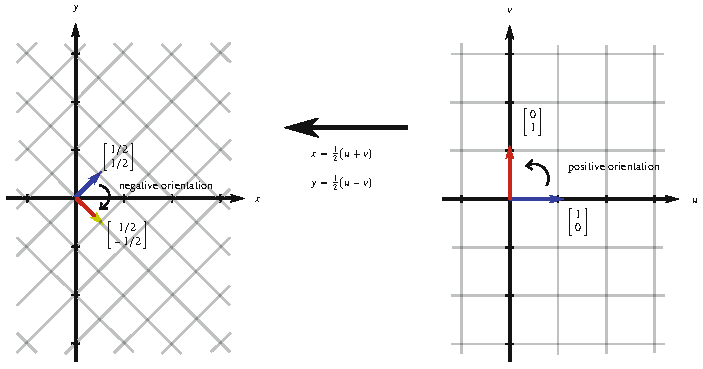
\includegraphics[width=0.960\linewidth]{images/vector/fig-6-6.pdf}
  \caption{$uv$ 平面中的基向量被映射为 $xy$ 平面中的两个向量. 注意定向发生变化}
  \label{fig:6-6}
\end{figure}

这同样与我们从图中预期的完全一致. 而且，我们开始更好地理解恒等式
\[
du\wedge dv=-2dx\wedge dy
\]
实际上是如何成立的：
\[
du\wedge dv\left(\binom{1}{0}_{uv(0,0)},\binom{0}{1}_{uv(0,0)}\right)
=-2dx\wedge dy\left(\binom{1/2}{1/2}_{xy(0,0)},\binom{1/2}{-1/2}_{xy(0,0)}\right).
\]
面积形式 $du\wedge dv$ 吃进来自 $uv$ 平面的向量，而面积形式 $dx\wedge dy$ 吃进来自 $xy$ 平面的向量. 此外，$dx\wedge dy$ 所吃进的向量，正是 $du\wedge dv$ 所吃进的向量在映射 $x$ 与 $y$（$x=\frac12(u+v)$ 与 $y=\frac12(u-v)$）下的投影. 所以我们的恒等式
\[
du\wedge dv=-2dx\wedge dy,\qquad dx\wedge dy=-\frac12du\wedge dv
\]
成立，但仅当它们所吃进的向量之间存在特定的关系时，也就是说，当它们所吃进的向量由两个空间之间的映射相关联时.

当然，在本节中我们犯了向量微积分的头号大罪，即把我们上面让体积形式所吃进的各个向量视为流形 $\mathbb{R}^2$ 的一部分，而不是它们实际上所在的 $T_{(0,0)}\mathbb{R}^2$ 的元素. 我们将在下一节纠正这一点. 本节的主要目的是试图更好地理解体积形式之间恒等式所涉及的微妙之处.

\section{向量的前推}

在上一节中我们考察了（线性坐标变换）映射
\[
f(x,y)=\bigl(u(x,y),v(x,y)\bigr):\mathbb{R}^2\to\mathbb{R}^2
\]
其中 $u(x,y)=x+y$ 与 $v(x,y)=x-y$. 然后我们用它们求出了恒等式 $du\wedge dv=-2dx\wedge dy$ 与 $dx\wedge dy=-\frac12du\wedge dv$，并开始探索这些恒等式实际上意味着什么. 它们与定义域流形 $\mathbb{R}^2$（用 $xy$ 坐标，我们记为 $\mathbb{R}^2_{xy}$）中的面积如何关联值域流形 $\mathbb{R}^2$（用 $uv$ 坐标，我们记为 $\mathbb{R}^2_{uv}$）中的面积有关. 我们发现，当 $du\wedge dv$ 所吃进的向量是 $dx\wedge dy$ 所吃进的向量在映射 $f(x,y)=\bigl(u(x,y),v(x,y)\bigr)=(x+y,x-y)$ 下的投影时，恒等式 $du\wedge dv=-2dx\wedge dy$ 成立. 类似地，当我们考虑逆映射时，我们发现当 $dx\wedge dy$ 所吃进的向量是 $du\wedge dv$ 所吃进的向量在逆映射下的投影时，恒等式 $dx\wedge dy=-\frac12du\wedge dv$ 成立. 然而，在这样做的时候，我们对用来确定平行六面体（我们求的是它们的体积）的向量相当不严谨. 如我们所知，向量实际上生活在切空间中，而不在流形中. 正如我们将看到的，我们在这里能够对这一事实一带而过，是因为这个映射是线性的.

并不是想用这个例子把你烦得要死，但在本节中我们将在数学上更精确的同时继续使用这个例子. 这将作为向量的前推这一思想的动机与引入. 在本章后面，这个例子还将作为微分形式的拉回这一思想的动机与引入. 此外，我们也想在引入像极坐标、球坐标或柱坐标这样更复杂的例子之前，先研究一个简单的例子.

接下来我们回想，流形 $\mathbb{R}^2_{xy}$（带 $xy$ 坐标）和流形 $\mathbb{R}^2_{uv}$（带 $uv$ 坐标），见图~\ref{fig:6-1}，在每个点处都有一个切空间，类似于图~\ref{fig:2-15} 所示的情况. 也就是说，如果 $(x,y)$ 是 $\mathbb{R}^2_{xy}$ 中的一个点，那么 $T_{(x,y)}\mathbb{R}^2_{xy}$ 就是 $\mathbb{R}^2_{xy}$ 在点 $(x,y)$ 处的切空间. 点 $f(x,y)=(x+y,x-y)$ 是点 $(x,y)$ 到 $\mathbb{R}^2_{uv}$ 的投影，而 $T_{(x+y,x-y)}\mathbb{R}^2_{uv}$ 是 $\mathbb{R}^2_{uv}$ 在投影点 $(x+y,x-y)$ 处的切空间.

另外，对于映射 $f(x,y)=\bigl(u(x,y),v(x,y)\bigr)=(x+y,x-y)$，$f$ 在点 $(x,y)$ 处的导数由 Jacobian 矩阵 $Df$ 给出：
\[
D_{(x,y)}f=
\begin{bmatrix}
\frac{\partial u}{\partial x}&\frac{\partial u}{\partial y}\\
\frac{\partial v}{\partial x}&\frac{\partial v}{\partial y}
\end{bmatrix}_{(x,y)}.
\]
让我们想一想 Jacobian 矩阵是什么、做什么. 它是函数 $f(x,y)$ 在点 $(x,y)$ 处最接近的线性逼近. 假设我们有某个以点 $(x,y)$ 为基点的向量 $v=\binom{a}{b}$. 这个向量实际上在 $\mathbb{R}^2_{xy}$ 在点 $(x,y)$ 处的切空间中，但暂时我们仍把它想成在流形 $\mathbb{R}^2_{xy}$ 中. 如果我们想知道当我们沿着向量 $v$ 从 $(x,y)$ 移动时 $f$ 改变了多少，我们可以求 $f(x,y)$ 和 $f(x+a,y+b)$ 来看出这一变化. 事实上，我们可以把这一变化想成从 $f(x,y)$ 到 $f(x+a,y+b)$ 的向量. 这里点 $(x,y)$ 和 $(x+a,y+b)$ 都在流形 $\mathbb{R}^2_{xy}$ 中，而点 $f(x,y)$ 和 $f(x+a,y+b)$ 都在流形 $\mathbb{R}^2_{uv}$ 中. 或者我们可以用 $f$ 在点 $(x,y)$ 处最接近的线性逼近来估计这一变化，它就是 $f$ 在点 $(x,y)$ 处的导数，由 Jacobian 矩阵 $Df$ 在点 $(x,y)$ 处给出. 要做到这一点，我们把 Jacobian 矩阵乘以向量 $v$，即求 $Df\cdot v$. 这给出另一个向量. 但这个向量在哪里呢？由于我们是在从点 $f(x,y)$ 处估计 $f$ 的变化，这个点就是我们新向量的基点，所以我们的新向量在 $\mathbb{R}^2_{uv}$ 在点 $f(x,y)$ 处的切空间中. 总而言之，Jacobian 矩阵实际上是一个映射
\[
D_{(x,y)}f:T_{(x,y)}\mathbb{R}^2_{xy}\longrightarrow T_{f(x,y)}\mathbb{R}^2_{uv}.
\]
出于我们稍后将解释的原因，我们通常用记号 $T_{(x,y)}f$ 表示在点 $(x,y)$ 处的 Jacobian 矩阵，而不是更常见的 $D_{(x,y)}f$. 对于我们的特定映射 $f(x,y)=\bigl(u(x,y),v(x,y)\bigr)=(x+y,x-y)$，我们有
\[
T_{(x,y)}f=
\begin{bmatrix}
\frac{\partial u}{\partial x}&\frac{\partial u}{\partial y}\\
\frac{\partial v}{\partial x}&\frac{\partial v}{\partial y}
\end{bmatrix}_{(x,y)}
=
\begin{bmatrix}
1&1\\
1&-1
\end{bmatrix}_{(x,y)}.
\]
例如，在点 $(0,0)$ 处向量 $\binom{1}{0}_{(0,0)}$ 被送到
\[
T_{(0,0)}f\cdot\binom{1}{0}_{(0,0)}
=
\begin{bmatrix}
1&1\\
1&-1
\end{bmatrix}_{(0,0)}
\cdot\binom{1}{0}_{(0,0)}
=
\binom{1}{1}_{f(0,0)=(0,0)},
\]
而向量 $\binom{0}{1}_{(0,0)}$ 被送到
\[
T_{(0,0)}f\cdot\binom{0}{1}_{(0,0)}
=
\begin{bmatrix}
1&1\\
1&-1
\end{bmatrix}_{(0,0)}
\cdot\binom{0}{1}_{(0,0)}
=
\binom{1}{-1}_{f(0,0)=(0,0)}.
\]
所以，从函数
\[
f:\mathbb{R}^2_{xy}\longrightarrow\mathbb{R}^2_{uv},\qquad p\longmapsto f(p)
\]
我们诱导出一个映射
\[
T_pf:T_p\mathbb{R}^2_{xy}\longrightarrow T_{f(p)}\mathbb{R}^2_{uv},\qquad
v_p\longmapsto T_pf\cdot v_p
\]
它从定义域流形 $\mathbb{R}^2_{xy}$ 的切丛到值域流形 $\mathbb{R}^2_{uv}$ 的切丛，无非就是 Jacobian 矩阵. 所谓"诱导"，我们的意思是我们用 $f$ 导出了另一个映射 $Tf$，而当我们把基点 $p$ 也考虑进去时，就得到 $T_pf$. 我们把 $T_pf\cdot v_p$ 称为 $v_p$ 被 $T_pf$ 的前推，而 $T_pf$ 有时被称为前推映射.

我们再做一例. 假设我们想求 $T_pf\cdot v_p$，其中
\[
v_p=\binom{1}{2}_{(1,1)}.
\]
首先我们求 $f(1,1)=(1+1,1-1)=(2,0)$. 接下来有
\[
T_{(1,1)}f\cdot\binom{1}{2}_{(1,1)}
=
\begin{bmatrix}
1&1\\
1&-1
\end{bmatrix}_{(1,1)}
\cdot\binom{1}{2}_{(1,1)}
=
\binom{3}{-1}_{f(1,1)}
=
\binom{3}{-1}_{(2,0)}.
\]
注意左边的基点是 $(1,1)$，而右边的基点是 $f(1,1)=(2,0)$.

\begin{question}\label{q:6-4}
用同一个函数 $f$，求下列向量的 $T_pf\cdot v_p$.
\begin{enumerate}
  \item[(a)] $v_p=\binom{-1}{-1}_{(5,4)}$
  \item[(b)] $v_p=\binom{-2}{3}_{(2,-3)}$
\end{enumerate}
\end{question}

由于 $f$ 已经是线性函数，$f$ 的 Jacobian 矩阵，即映射 $T_pf$，在每个点处都相同. 我们很快就会遇到并非如此的例子. 但还有别的东西值得注意. 考虑一个一般向量 $v_p=\binom{x}{y}_p$. 则
\[
T_pf\cdot\binom{x}{y}_p
=
\begin{bmatrix}
1&1\\
1&-1
\end{bmatrix}_p
\cdot\binom{x}{y}_p
=
\binom{x+y}{x-y}_{f(p)}.
\]
我们有，$T_pf$ 作用于 $\binom{x}{y}_p\in T_p\mathbb{R}^2$（其中 $p\in$ 流形 $\mathbb{R}^2$），看起来与函数 $f$ 作用于 $(x,y)\in$ 流形 $\mathbb{R}^2$ 完全相同：
\[
f(x,y)=(x+y,x-y)\in\mathbb{R}^2,\qquad
T_pf\cdot\binom{x}{y}_p=\binom{x+y}{x-y}_{f(p)}\in T_{f(p)}\mathbb{R}^2,\ p\in\mathbb{R}^2.
\]
当然，$Tf$ 与 $f$ 的定义域和值域是不同的空间，但函数 $Tf$ 与 $f$ 作用于输入点的方式看起来是一样的. 对于线性函数 $f$，你经常会看到人们写下
\[
Tf=f.
\]
显然，由于定义域和值域不同，这在技术上不可能成立，但这是一个方便的所谓"记号的滥用". （实际上，记号的滥用（abuse of notation）在数学中极其常见. 当你最初学习某个东西时，这些记号的滥用常常会妨碍理解，但一旦你理解了正在发生的事情，它们就使计算和记录变得如此简单而快速. 总是绝对精确会让人难以承受，也不必要地困难，而且对真正理解事情的人来说没有必要.）

把我们刚刚学到的东西付诸使用，我们将重做上一节所做的事情. 坚持使用同一个函数 $f(x,y)=\bigl(u(x,y),v(x,y)\bigr)=(x+y,x-y)$，考虑点 $(5,7)\in\mathbb{R}^2_{xy}$. 我们求出 $f(5,7)=(5+7,5-7)=(12,-2)$. 接下来，我们求由该点处的欧几里得单位向量
\[
\binom{1}{0}_{(5,7)},\qquad\binom{0}{1}_{(5,7)}\in T_{(5,7)}\mathbb{R}^2_{xy}
\]
张成的平行六面体的面积. 严格地说，这个平行六面体位于切空间 $T_{(5,7)}\mathbb{R}^2_{xy}$ 中，但鉴于我们可以把切空间与底层的流形 $\mathbb{R}^2_{xy}$ 自然地等同起来，我们常常也把这个平行六面体想成在流形中. 用我们的面积形式 $dx\wedge dy$，我们得到面积为
\[
(dx\wedge dy)_{(5,7)}\left(\binom{1}{0}_{(5,7)},\binom{0}{1}_{(5,7)}\right)=\left|\begin{matrix}1&0\\0&1\end{matrix}\right|=1.
\]
接下来我们用 $T_{(5,7)}f$ 把这些向量前推到空间 $T_{(12,-2)}\mathbb{R}^2_{uv}$：
\begin{align*}
T_{(5,7)}f\cdot\binom{1}{0}_{(5,7)}
=
\begin{bmatrix}
1&1\\
1&-1
\end{bmatrix}
\cdot\binom{1}{0}_{(5,7)}
=
\binom{1}{1}_{(12,-2)}\in T_{(12,-2)}\mathbb{R}^2_{uv}, \\
T_{(5,7)}f\cdot\binom{0}{1}_{(5,7)}
=
\begin{bmatrix}
1&1\\
1&-1
\end{bmatrix}
\cdot\binom{0}{1}_{(5,7)}
=
\binom{1}{-1}_{(12,-2)}\in T_{(12,-2)}\mathbb{R}^2_{uv}.
\end{align*}
现在我们用面积形式 $du\wedge dv$ 求由这些被前推的向量张成的平行六面体的面积：
\[
(du\wedge dv)_{(12,-2)}\left(T_{(5,7)}f\cdot\binom{1}{0}_{(5,7)},T_{(5,7)}f\cdot\binom{0}{1}_{(5,7)}\right)
=\left|\begin{matrix}1&1\\1&-1\end{matrix}\right|=-1-1=-2.
\]
总而言之，对 $p=(5,7)$ 我们求出
\[
(dx\wedge dy)_p\underbrace{\left(\binom{1}{0}_p,\binom{0}{1}_p\right)}_{\text{$T_p\mathbb{R}^2_{xy}$ 中的向量}}=1
\]
以及
\[
(du\wedge dv)_{f(p)}\underbrace{\left(T_pf\cdot\binom{1}{0}_p,T_pf\cdot\binom{0}{1}_p\right)}_{\substack{\text{$T_p\mathbb{R}^2_{xy}$ 中向量的前推，}\\\text{位于 $T_{f(p)}\mathbb{R}^2_{uv}$ 中}}}=-2
\]
把一切结合起来，我们得到如下等式
\[
\underbrace{-2\cdot\underbrace{(dx\wedge dy)_p\left(\binom{1}{0}_p,\binom{0}{1}_p\right)}_{=1}}_{=-2}
=
(du\wedge dv)_{f(p)}\underbrace{\left(T_pf\cdot\binom{1}{0}_p,T_pf\cdot\binom{0}{1}_p\right)}_{=-2}
\]
这正是我们在上一节得到的，只是认识到 $du\wedge dv$ 所吃进的向量是 $dx\wedge dy$ 所吃进的向量的前推. 所以，为了严格地理解恒等式 $-2dx\wedge dy=du\wedge dv$，我们需要处理的概念就是向量的前推.

\begin{question}\label{q:6-5}
考虑同一个坐标变换 $f(x,y)=\bigl(u(x,y),v(x,y)\bigr)=(x+y,x-y)$.
\begin{enumerate}
  \item[(a)] 求 $f(3,-2)$.
  \item[(b)] 求 $(dx\wedge dy)_{(3,-2)}\left(\binom{1}{1}_{(3,-2)},\binom{5}{-1}_{(3,-2)}\right)$.
  \item[(c)] 求 $T_{(3,-2)}f\cdot\binom{1}{1}_{(3,-2)}$ 与 $T_{(3,-2)}f\cdot\binom{5}{-1}_{(3,-2)}$.
  \item[(d)] 求 $(du\wedge dv)_{f(3,-2)}\left(T_{(3,-2)}f\cdot\binom{1}{1}_{(3,-2)},T_{(3,-2)}f\cdot\binom{5}{-1}_{(3,-2)}\right)$.
  \item[(e)] 答案与你从最后一个例子以及关系式 $dx\wedge dy=-\frac12du\wedge dv$ 所预期的一致吗？
\end{enumerate}
\end{question}

现在我们稍微一般化一点，在比我们特定问题更一般的背景下简要考察向量的前推. 考虑两个流形之间的映射 $f:M\to N$. 暂时我们把自己限制在 $M=N=\mathbb{R}^n$（对某个 $n$）的情形. 如果映射 $f=(f_1,f_2,\ldots,f_n)$ 在点 $p\in M$ 处可微（这意味着每个 $f_i$ 都在 $p$ 处可微），且流形 $M$ 的坐标由 $x_1,x_2,\ldots,x_n$ 给出，那么该映射在点 $p\in M$ 处的导数由传统的 Jacobian 矩阵给出：
\[
T_pf=\text{$f$ 在 $p$ 处的 Jacobian 矩阵}
=
\begin{bmatrix}
\frac{\partial f_1}{\partial x_1}\Big|_p&\frac{\partial f_1}{\partial x_2}\Big|_p&\cdots&\frac{\partial f_1}{\partial x_n}\Big|_p\\
\frac{\partial f_2}{\partial x_1}\Big|_p&\frac{\partial f_2}{\partial x_2}\Big|_p&\cdots&\frac{\partial f_2}{\partial x_n}\Big|_p\\
\vdots&\vdots&\ddots&\vdots\\
\frac{\partial f_n}{\partial x_1}\Big|_p&\frac{\partial f_n}{\partial x_2}\Big|_p&\cdots&\frac{\partial f_n}{\partial x_n}\Big|_p
\end{bmatrix}.
\]
由 Jacobian 矩阵给出的映射 $T_pf$ 就是映射 $f:M\to N$ 最接近的线性逼近. 我们已经花了大量时间考虑实值函数 $g:\mathbb{R}^n\to\mathbb{R}$ 与微分 $dg$. 我们知道 $g$ 在点 $p$ 处的微分实际上是 $g$ 在点 $p$ 处最接近的线性逼近. 事实上，我们说过 $dg_p$ 在某种意义上"编码"了 $g$ 在点 $p$ 处的切平面，而当然 $g$ 在点 $p$ 处的切平面就是 $g$ 的图像最接近的线性逼近. 利用笛卡尔坐标，我们可以把 $g$ 的微分写成
\[
dg=\frac{\partial g}{\partial x_1}dx_1+\frac{\partial g}{\partial x_2}dx_2+\cdots+\frac{\partial g}{\partial x_n}dx_n
=\left[\frac{\partial g}{\partial x_1},\frac{\partial g}{\partial x_2},\cdots,\frac{\partial g}{\partial x_n}\right].
\]
在我们的函数 $f=(f_1,f_2,\ldots,f_n)$ 的情形下，每个分量函数 $f_i$ 本身是一个实值函数 $f_i:\mathbb{R}^n\to\mathbb{R}$，因此我们可以分别考虑每个 $f_i$ 的微分：
\begin{align*}
df_1=\frac{\partial f_1}{\partial x_1}dx_1+\frac{\partial f_1}{\partial x_2}dx_2+\cdots+\frac{\partial f_1}{\partial x_n}dx_n
=\left[\frac{\partial f_1}{\partial x_1},\frac{\partial f_1}{\partial x_2},\cdots,\frac{\partial f_1}{\partial x_n}\right], \\
df_2=\frac{\partial f_2}{\partial x_1}dx_1+\frac{\partial f_2}{\partial x_2}dx_2+\cdots+\frac{\partial f_2}{\partial x_n}dx_n
=\left[\frac{\partial f_2}{\partial x_1},\frac{\partial f_2}{\partial x_2},\cdots,\frac{\partial f_2}{\partial x_n}\right], \\
\vdots \\
df_n=\frac{\partial f_n}{\partial x_1}dx_1+\frac{\partial f_n}{\partial x_2}dx_2+\cdots+\frac{\partial f_n}{\partial x_n}dx_n
=\left[\frac{\partial f_n}{\partial x_1},\frac{\partial f_n}{\partial x_2},\cdots,\frac{\partial f_n}{\partial x_n}\right].
\end{align*}
把 $f$ 的各分量函数的余向量与 Jacobian 矩阵的行进行比较. 它们是相同的. 因此，$f$ 的 Jacobian 矩阵的行无非是 $f$ 的各分量函数的微分 $df_i$ 写成行矩阵. Jacobian 矩阵 $Tf$ 是映射 $f:\mathbb{R}^n\to\mathbb{R}^n$ 最接近的线性逼近，因为它的行是每个 $f_i:\mathbb{R}^n\to\mathbb{R}$ 最接近的线性逼近.

\begin{figure}[htbp]
  \centering
  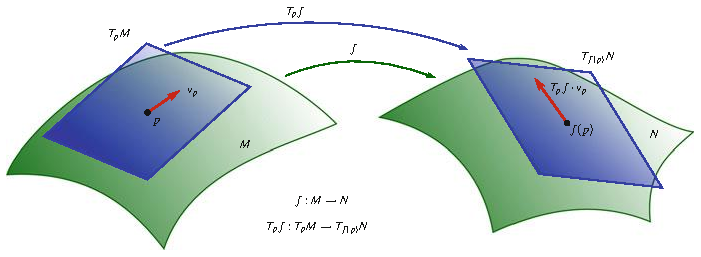
\includegraphics[width=0.960\linewidth]{images/vector/fig-6-7.pdf}
  \caption{映射 $f:M\to N$ 诱导切映射 $Tf:TM\to TN$. 在特定点 $p\in M$ 处我们得到 $T_pf:T_pM\to T_{f(p)}N$. 于是向量 $v_p\in T_pM$ 被前推到向量 $T_pf\cdot v_p\in T_{f(p)}N$}
  \label{fig:6-7}
\end{figure}

和之前一样，假设我们有某个向量 $v_p\in T_pM$. $T_pf\cdot v_p$ 给出当我们沿着 $v_p$ 移动时 $f$ 的变化的线性逼近，它是 $T_{f(p)}N$ 中的另一个向量. 由于我们可以在 $f$ 可微的每个点 $p\in M$ 处求出 $T_pf:T_pM\to T_{f(p)}N$，我们最终得到从 $M$ 的切丛到 $N$ 的切丛的映射 $Tf$. 我们说映射 $f:M\to N$ 诱导映射 $Tf:TM\to TN$. 映射 $Tf$ 把 $T_pM$ 中的向量前推到 $T_{f(p)}N$ 中的向量. 这个映射通常称为由 $f$ 诱导的\newterm{tangent-map}{切映射}{tangent map}. 见图~\ref{fig:6-7}. 我们常常会这样展示，写出类似下面的东西：
\[
\begin{gathered}
TM\xrightarrow{\substack{Tf\\f_*\\Df}}TN\\
v\longmapsto Tf\cdot v\\
M\xrightarrow{f}N\\
p\longmapsto f(p).
\end{gathered}
\]
你会遇到这个诱导映射的三种不同记号：$D_pf$、$T_pf$ 和 $f_*(p)$. $D_pf$ 是相当标准的记号，你会经常遇到它，尤其是在微积分课上. 然而，大概最常用的记号是 $f_*$. 如果我们想包含基点，它常常被写成 $f_*(p)$，这有点笨拙. 这个记号在微分几何书籍中最常遇到. 然而，一般来说我们将使用记号 $Tf$ 或 $T_pf$. 坦白地说，这是一个相当非标准的记号，但我们喜欢它，因为作为一种记号，它包含了大量信息. $Tf$ 中的 $T$ 告诉我们，我们在处理由映射 $f$ 诱导的、从一个切丛到另一个切丛的切映射. 这个记号还可以在我们想要的时候把基点 $p$ 漂亮地包含进去，其方式与切空间记号中包含基点的方式相同. 因此，$T_pf$ 用来指明从切空间 $T_pM$ 到切空间 $T_{f(p)}N$ 的映射.

\section{体积形式的拉回}

在本节中我们将定义体积形式的拉回. 虽然大多数微分形式并不是体积形式，但体积形式在积分中扮演着非常重要的角色，所以我们在本节中将集中于它们. 我们将在后面探讨更一般微分形式的拉回. 目前我们将继续我们的线性例子. 我们的基本目标是把关系式
\[
\underbrace{-2\cdot\underbrace{(dx\wedge dy)_p\left(\binom{1}{0}_p,\binom{0}{1}_p\right)}_{=1}}_{=-2}
=
(du\wedge dv)_{f(p)}\underbrace{\left(T_pf\cdot\binom{1}{0}_p,T_pf\cdot\binom{0}{1}_p\right)}_{=-2}
\]
理解得更精确一些.

回想对于映射 $f(x,y)=(x+y,x-y)$ 我们有
\begin{align*}
du\wedge dv&=d(x+y)\wedge d(x-y)\\
&=(dx+dy)\wedge(dx-dy)\\
&=dx\wedge(dx-dy)+dy\wedge(dx-dy)\\
&=dx\wedge dx-dx\wedge dy+dy\wedge dx-dy\wedge dy\\
&=-dx\wedge dy-dx\wedge dy\\
&=-2dx\wedge dy.
\end{align*}
我们一般性地重做这个计算. 也就是说，考虑由 $f(x,y)=\bigl(u(x,y),v(x,y)\bigr)=(u,v)$ 给出的换元 $f:\mathbb{R}^2_{xy}\to\mathbb{R}^2_{uv}$. 首先我们求
\[
du=\frac{\partial u}{\partial x}dx+\frac{\partial u}{\partial y}dy,\qquad
dv=\frac{\partial v}{\partial x}dx+\frac{\partial v}{\partial y}dy,
\]
然后利用楔积的性质得到
\begin{align*}
du\wedge dv&=\left(\frac{\partial u}{\partial x}dx+\frac{\partial u}{\partial y}dy\right)\wedge\left(\frac{\partial v}{\partial x}dx+\frac{\partial v}{\partial y}dy\right)\\
&=\frac{\partial u}{\partial x}dx\wedge\left(\frac{\partial v}{\partial x}dx+\frac{\partial v}{\partial y}dy\right)
+\frac{\partial u}{\partial y}dy\wedge\left(\frac{\partial v}{\partial x}dx+\frac{\partial v}{\partial y}dy\right)\\
&=\frac{\partial u}{\partial x}\frac{\partial v}{\partial x}\underbrace{dx\wedge dx}_{=0}
+\frac{\partial u}{\partial x}\frac{\partial v}{\partial y}dx\wedge dy
+\frac{\partial u}{\partial y}\frac{\partial v}{\partial x}\underbrace{dy\wedge dx}_{-dx\wedge dy}
+\frac{\partial u}{\partial y}\frac{\partial v}{\partial y}\underbrace{dy\wedge dy}_{=0}\\
&=\frac{\partial u}{\partial x}\frac{\partial v}{\partial y}dx\wedge dy-\frac{\partial u}{\partial y}\frac{\partial v}{\partial x}dx\wedge dy\\
&=\left(\frac{\partial u}{\partial x}\frac{\partial v}{\partial y}-\frac{\partial u}{\partial y}\frac{\partial v}{\partial x}\right)dx\wedge dy\\
&=\underbrace{\left|\begin{matrix}\frac{\partial u}{\partial x}&\frac{\partial u}{\partial y}\\\frac{\partial v}{\partial x}&\frac{\partial v}{\partial y}\end{matrix}\right|}_{\text{Jacobian 矩阵的行列式}}dx\wedge dy.
\end{align*}
本质上看来，当我们在求两个体积形式之间的关系时，Jacobian 矩阵就是"自然而然地蹦出来"的. 在上一节中，我们试图通过引入诱导切映射 $Tf$ 和向量的前推这一思想来更好地理解这个恒等式的含义. 诱导切映射 $Tf$ 按照下式作用：
\[
\begin{gathered}
T_p\mathbb{R}^2\xrightarrow{T_pf}T_{f(p)}\mathbb{R}^2\\
\mathbb{R}^2\xrightarrow{f}\mathbb{R}^2,
\end{gathered}
\]
其中在 $p$ 处的切映射 $T_pf$ 由在 $p$ 处求值的 Jacobian 矩阵给出：
\[
T_pf=
\begin{bmatrix}
\frac{\partial u}{\partial x}&\frac{\partial u}{\partial y}\\
\frac{\partial v}{\partial x}&\frac{\partial v}{\partial y}
\end{bmatrix}_p.
\]
我们把向量 $v_p=\binom{v_1}{v_2}_p\in T_p\mathbb{R}^2$ 的前推定义为
\[
T_pf\cdot v_p=
\begin{bmatrix}
\frac{\partial u}{\partial x}&\frac{\partial u}{\partial y}\\
\frac{\partial v}{\partial x}&\frac{\partial v}{\partial y}
\end{bmatrix}_p
\cdot\binom{v_1}{v_2}_p
=
\begin{bmatrix}
\frac{\partial u}{\partial x}v_1+\frac{\partial u}{\partial y}v_2\\
\frac{\partial v}{\partial x}v_1+\frac{\partial v}{\partial y}v_2
\end{bmatrix}_{f(p)}
\in T_{f(p)}\mathbb{R}^2.
\]
把基点 $p$ 从我们的计算中略去，并在方便之处用 $\det$ 表示行列式，我们有
\begin{align*}
du\wedge dv(Tf\cdot v,Tf\cdot w)
&=\det\begin{bmatrix}du(Tf\cdot v)&du(Tf\cdot w)\\dv(Tf\cdot v)&dv(Tf\cdot w)\end{bmatrix}\\
&=\det\begin{bmatrix}\frac{\partial u}{\partial x}v_1+\frac{\partial u}{\partial y}v_2&\frac{\partial u}{\partial x}w_1+\frac{\partial u}{\partial y}w_2\\[2pt]\frac{\partial v}{\partial x}v_1+\frac{\partial v}{\partial y}v_2&\frac{\partial v}{\partial x}w_1+\frac{\partial v}{\partial y}w_2\end{bmatrix}\\
&=\det\left(\begin{bmatrix}\frac{\partial u}{\partial x}&\frac{\partial u}{\partial y}\\\frac{\partial v}{\partial x}&\frac{\partial v}{\partial y}\end{bmatrix}\begin{bmatrix}v_1&w_1\\v_2&w_2\end{bmatrix}\right)\\
&=\det\begin{bmatrix}\frac{\partial u}{\partial x}&\frac{\partial u}{\partial y}\\\frac{\partial v}{\partial x}&\frac{\partial v}{\partial y}\end{bmatrix}\cdot\det\begin{bmatrix}v_1&w_1\\v_2&w_2\end{bmatrix}\\
&=\left|\begin{matrix}\frac{\partial u}{\partial x}&\frac{\partial u}{\partial y}\\\frac{\partial v}{\partial x}&\frac{\partial v}{\partial y}\end{matrix}\right|\cdot\left|\begin{matrix}dx(v)&dx(w)\\dy(v)&dy(w)\end{matrix}\right|\\
&=\left|\begin{matrix}\frac{\partial u}{\partial x}&\frac{\partial u}{\partial y}\\\frac{\partial v}{\partial x}&\frac{\partial v}{\partial y}\end{matrix}\right|dx\wedge dy(v,w)
\end{align*}
这给我们恒等式
\[
\left|\begin{matrix}\frac{\partial u}{\partial x}&\frac{\partial u}{\partial y}\\\frac{\partial v}{\partial x}&\frac{\partial v}{\partial y}\end{matrix}\right|dx\wedge dy(v,w)
=du\wedge dv(Tf\cdot v,Tf\cdot w).
\]
再次地，当我们计算面积形式在由 $f$ 给出的基变换下如何变化时，Jacobian 矩阵基本上"自然而然地蹦出来了". 但同样，Jacobian 矩阵恰恰就是我们在换基时把向量前推的那个 $Tf$，而向量（或向量的前推）显然是求由向量张成的平行六面体的面积所必需的. 就好像 Jacobian 矩阵在某种意义上"贯穿"了整个计算.

现在我们定义什么是微分形式的拉回. 记住，在本节中我们真正考察过的唯一微分形式就是体积形式，因为它对积分很重要. 但这个基本定义实际上适用于所有微分形式. 假设我们有流形之间的映射 $f:M\to N$. 这个映射诱导切映射 $Tf:TM\to TN$. 现在假设我们在 $N$ 上有一个微分 $k$-形式 $\omega$. 那么我们定义微分 $k$-形式 $T^*f\cdot\omega$ 为 $\omega$ 到 $M$ 的拉回，其中

\begin{definition}[微分形式的拉回]\label{def:6-3-1}
\[
\bigl(T^*f\cdot\omega\bigr)(v_1,v_2,\ldots,v_k)=\omega\bigl(Tf\cdot v_1,Tf\cdot v_2,\ldots,Tf\cdot v_k\bigr).
\]
\end{definition}

这到底想说什么？如果我们给定 $N$（即 $f$ 的值域）上的一个 $k$-形式 $\omega$，那么我们试图求 $M$ 上在某种意义上与 $\omega$"相同"的 $k$-形式. 我们所说的"相同"是什么意思？这两个形式所要吃进的向量来自不同的切空间. 但我们已经知道，$M$ 上的切向量可以用自然的方式前推到 $N$ 上的切向量，所以我们决定利用这一思想. 当我们试图求的 $M$ 上的 $k$-形式吃进 $k$ 个切向量时，我们希望它给出的值，与 $N$ 上的 $k$-形式 $\omega$ 吃进这些同样的向量的前推时给出的值相同. 我们求出的 $M$ 上的这个 $k$-形式记为 $T^*f\cdot\omega$ 或 $f^*\omega$，称为 $\omega$ 的拉回. 最常用的记号是 $f^*$，但出于在切向量的前推那一节中解释过的同样的原因，我们将使用 $T^*f$. 拉回映射有时也称为\newterm{cotangent-map}{余切映射}{cotangent map}.

\begin{figure}[htbp]
  \centering
  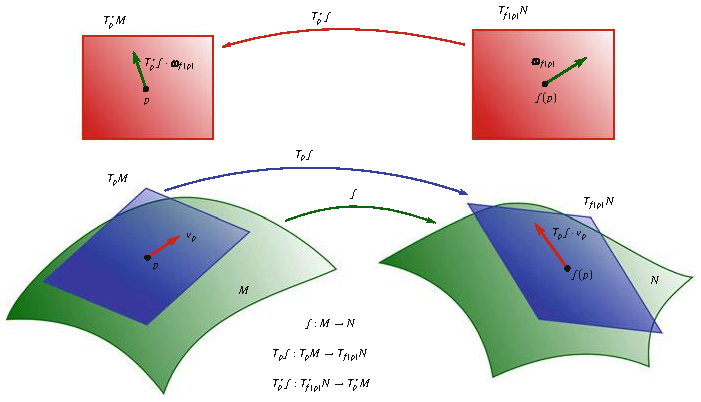
\includegraphics[width=0.960\linewidth]{images/vector/fig-6-8.pdf}
  \caption{映射 $f$ 与 $Tf$ 如图~\ref{fig:6-7} 所示，但现在还包含了拉回映射 $T^*f:T^*N\to T^*M$. 在特定点 $f(p)\in N$ 处我们有 $T_p^*f:T_{f(p)}^*N\to T_p^*M$. 注意映射 $T_p^*f$ 实际上是以值域中的点 $p$ 为下标的. 这相当不寻常，但这样做有助于保持记号一致}
  \label{fig:6-8}
\end{figure}

在这里我们连同基点记号一起展示所有这些映射. 见图~\ref{fig:6-8}. 有一件非常重要的事情值得注意：说到拉回映射，它是按像中的基点而不是定义域中的基点加下标的！这在数学中相当不寻常，但在这种情形下，它恰好是跟踪基点最好的方式. 我们常常把映射 $f$ 及其诱导映射 $T_pf$ 与 $T_p^*f$ 写成
\[
\begin{gathered}
\bigwedge_p^k(M)\xleftarrow{T_p^*f}\bigwedge_{f(p)}^k(N)\\
T_p^*f\cdot\omega_{f(p)}\longleftarrow\omega_{f(p)}\\
T_pM\xrightarrow{T_pf}T_{f(p)}N\\
v_p\longmapsto T_{f(p)}f\cdot v_p\\
M\xrightarrow{f}N\\
p\longmapsto f(p).
\end{gathered}
\]
现在我们准备理解我们的例子中发生的事情. 这里一切都被放在一起：
\[
\underbrace{\left|\begin{matrix}1&1\\1&-1\end{matrix}\right|\cdot(dx\wedge dy)_p}_{=\ (-2)(1)=-2}
\underbrace{\left(\binom{1}{0}_p,\binom{0}{1}_p\right)}_{\text{$T_p\mathbb{R}^2_{xy}$ 中的向量}}
=
(du\wedge dv)_{f(p)}\underbrace{\left(T_pf\cdot\binom{1}{0}_p,T_pf\cdot\binom{0}{1}_p\right)}_{\text{$T_p\mathbb{R}^2_{xy}$ 中向量的前推，位于 $T_{f(p)}\mathbb{R}^2_{uv}$ 中}}
\]
恒等式 $-2dx\wedge dy=du\wedge dv$ 真正正确的写法是：2-形式 $-2dx\wedge dy$ 是 $du\wedge dv$ 的拉回，
\[
T^*f\cdot\bigl(du\wedge dv\bigr)=-2dx\wedge dy.
\]

正如我们前面所说，在本节中我们主要集中讨论体积形式，因为它们对积分的作用. 现在我们将在完全一般性下考虑体积的拉回. 我们想求体积形式在坐标变换映射
\[
\phi:\mathbb{R}^n_{(x_1,\ldots,x_n)}\to\mathbb{R}^n_{(\phi_1,\ldots,\phi_n)}
\]
下的拉回，其中
\[
\phi=\bigl(\phi_1(x_1,\ldots,x_n),\phi_2(x_1,\ldots,x_n),\ldots,\phi_n(x_1,\ldots,x_n)\bigr).
\]
现在考虑 $\mathbb{R}^n_{(\phi_1,\ldots,\phi_n)}$ 上的体积形式 $\omega=d\phi_1\wedge d\phi_2\wedge\cdots\wedge d\phi_n$. 我们想求 $\mathbb{R}^n_{(x_1,\ldots,x_n)}$ 上 $T^*\phi\cdot\omega$ 的一般公式. 显然，我们知道 $T^*\phi\cdot\omega$ 也将是一个 $n$-形式，因此它必须具有形式 $f\,dx_1\wedge dx_2\wedge\cdots\wedge dx_n$，其中 $f$ 是某个迄今未知的函数. 令
\[
e_1=\begin{bmatrix}1\\0\\0\\\vdots\\0\end{bmatrix},\qquad
e_2=\begin{bmatrix}0\\1\\0\\\vdots\\0\end{bmatrix},\qquad\ldots,\qquad
e_n=\begin{bmatrix}0\\\vdots\\0\\0\\1\end{bmatrix},
\]
我们有
\[
dx_1\wedge dx_2\wedge\cdots\wedge dx_n(e_1,e_2,\ldots,e_n)=1.
\]
另外，回想
\[
T\phi=
\begin{bmatrix}
\frac{\partial\phi_1}{\partial x_1}&\frac{\partial\phi_1}{\partial x_2}&\cdots&\frac{\partial\phi_1}{\partial x_n}\\
\frac{\partial\phi_2}{\partial x_1}&\frac{\partial\phi_2}{\partial x_2}&\cdots&\frac{\partial\phi_2}{\partial x_n}\\
\vdots&\vdots&\ddots&\vdots\\
\frac{\partial\phi_n}{\partial x_1}&\frac{\partial\phi_n}{\partial x_2}&\cdots&\frac{\partial\phi_n}{\partial x_n}
\end{bmatrix}
\]
我们有
\[
T\phi\cdot e_1=\begin{bmatrix}\frac{\partial\phi_1}{\partial x_1}\\\frac{\partial\phi_2}{\partial x_1}\\\vdots\\\frac{\partial\phi_n}{\partial x_1}\end{bmatrix},\qquad
T\phi\cdot e_2=\begin{bmatrix}\frac{\partial\phi_1}{\partial x_2}\\\frac{\partial\phi_2}{\partial x_2}\\\vdots\\\frac{\partial\phi_n}{\partial x_2}\end{bmatrix},\qquad\ldots,\qquad
T\phi\cdot e_n=\begin{bmatrix}\frac{\partial\phi_1}{\partial x_n}\\\frac{\partial\phi_2}{\partial x_n}\\\vdots\\\frac{\partial\phi_n}{\partial x_n}\end{bmatrix}
\]
所以我们得到
\begin{align*}
f&=\bigl(f\,dx_1\wedge dx_2\wedge\cdots\wedge dx_n\bigr)(e_1,e_2,\ldots,e_n)\\
&=\bigl(T^*\phi\cdot\omega\bigr)(e_1,e_2,\ldots,e_n)\\
&=\omega\bigl(T\phi\cdot e_1,T\phi\cdot e_2,\ldots,T\phi\cdot e_n\bigr)\\
&=d\phi_1\wedge d\phi_2\wedge\cdots\wedge d\phi_n\bigl(T\phi\cdot e_1,T\phi\cdot e_2,\ldots,T\phi\cdot e_n\bigr)\\
&=\left|\begin{matrix}
d\phi_1(T\phi\cdot e_1)&d\phi_1(T\phi\cdot e_2)&\cdots&d\phi_1(T\phi\cdot e_n)\\
d\phi_2(T\phi\cdot e_1)&d\phi_2(T\phi\cdot e_2)&\cdots&d\phi_2(T\phi\cdot e_n)\\
\vdots&\vdots&\ddots&\vdots\\
d\phi_n(T\phi\cdot e_1)&d\phi_n(T\phi\cdot e_2)&\cdots&d\phi_n(T\phi\cdot e_n)
\end{matrix}\right|\\
&=\left|\begin{matrix}
\frac{\partial\phi_1}{\partial x_1}&\frac{\partial\phi_1}{\partial x_2}&\cdots&\frac{\partial\phi_1}{\partial x_n}\\
\frac{\partial\phi_2}{\partial x_1}&\frac{\partial\phi_2}{\partial x_2}&\cdots&\frac{\partial\phi_2}{\partial x_n}\\
\vdots&\vdots&\ddots&\vdots\\
\frac{\partial\phi_n}{\partial x_1}&\frac{\partial\phi_n}{\partial x_2}&\cdots&\frac{\partial\phi_n}{\partial x_n}
\end{matrix}\right|.
\end{align*}
把一切结合起来，我们得到体积形式在基变换 $\phi:\mathbb{R}^n_{(x_1,\ldots,x_n)}\to\mathbb{R}^n_{(\phi_1,\ldots,\phi_n)}$ 下拉回的一般公式为

\begin{definition}[体积形式的拉回]\label{def:6-3-2}
\[
T^*\phi\cdot\bigl(d\phi_1\wedge d\phi_2\wedge\cdots\wedge d\phi_n\bigr)
=\left|\begin{matrix}
\frac{\partial\phi_1}{\partial x_1}&\frac{\partial\phi_1}{\partial x_2}&\cdots&\frac{\partial\phi_1}{\partial x_n}\\
\frac{\partial\phi_2}{\partial x_1}&\frac{\partial\phi_2}{\partial x_2}&\cdots&\frac{\partial\phi_2}{\partial x_n}\\
\vdots&\vdots&\ddots&\vdots\\
\frac{\partial\phi_n}{\partial x_1}&\frac{\partial\phi_n}{\partial x_2}&\cdots&\frac{\partial\phi_n}{\partial x_n}
\end{matrix}\right|dx_1\wedge dx_2\wedge\cdots\wedge dx_n.
\]
\end{definition}

至少当涉及到同维流形之间的映射时，体积形式的拉回具有一个用坐标变换映射 $\phi$ 表示的非常漂亮的形式. 本质上，用于向量场前推的 Jacobian 矩阵 $T\phi$ 贯穿了整个体积形式计算. 然而，我们要告诫你，对更一般的 $k$-形式，没有求拉回的好公式. 这个涉及 Jacobian 矩阵的、对体积形式拉回来说格外精彩的公式，只适用于体积形式，且只适用于同维流形之间的映射.

\section{极坐标}

首先我们将探讨由
\[
f(r,\theta)=\bigl(x(r,\theta),y(r,\theta)\bigr)=\bigl(r\cos\theta,r\sin\theta\bigr)
\]
给出的极坐标变换 $f:\mathbb{R}^2_{r\theta}\to\mathbb{R}^2_{xy}$，它在微积分教科书中常常写成
\[
x=r\cos\theta,\qquad y=r\sin\theta.
\]
逆变换 $f^{-1}:\mathbb{R}^2_{xy}\to\mathbb{R}^2_{r\theta}$ 由更难看的
\[
f^{-1}(x,y)=\bigl(r(x,y),\theta(x,y)\bigr)=\left(\pm\sqrt{x^2+y^2},\arctan\frac{y}{x}\right)
\]
给出，其中当 $x\geq0$ 时取 $+$，当 $x<0$ 时取 $-$，且 $\theta$ 被限制在 $-\frac{\pi}{2}<\theta<\frac{\pi}{2}$，即 $\arctan$ 有定义的区间. 这一限制也使原函数成为一一映射. 这也可以写成
\[
r=\pm\sqrt{x^2+y^2},\qquad \theta=\arctan\frac{y}{x}
\]
并如图~\ref{fig:6-9} 所示.

\begin{figure}[htbp]
  \centering
  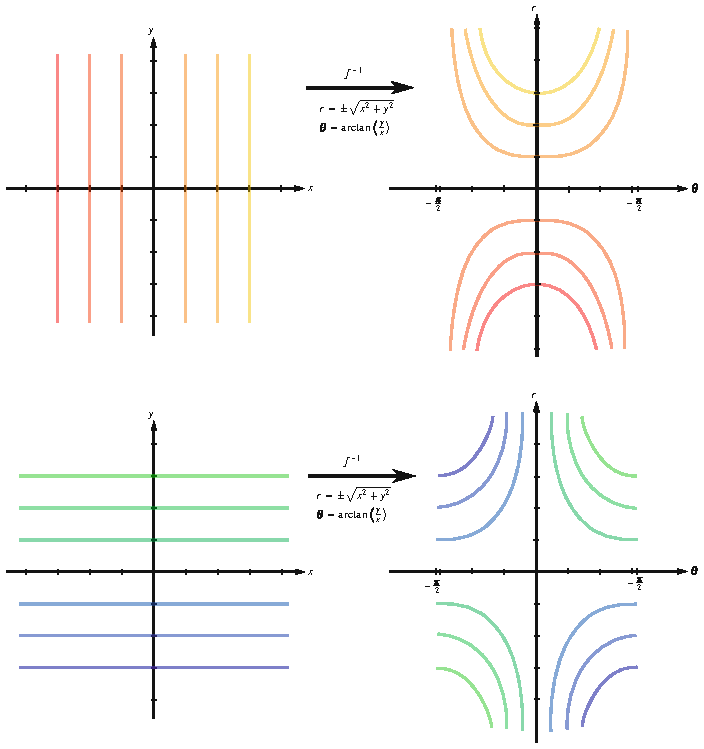
\includegraphics[width=0.960\linewidth]{images/vector/fig-6-9.pdf}
  \caption{极坐标变换 $f^{-1}:\mathbb{R}^2_{xy}\to\mathbb{R}^2_{r\theta}$ 被限制在 $-\pi/2<\theta\leq\pi/2$ 上. 这一限制是使 $f^{-1}$ 成为一一映射所必需的. 顶部显示了若干竖直直线的像，底部显示了若干水平直线的像}
  \label{fig:6-9}
\end{figure}

\begin{question}\label{q:6-6}
证明 $f^{-1}(x,y)$ 确实由 $f^{-1}(x,y)=\left(\pm\sqrt{x^2+y^2},\arctan\frac{y}{x}\right)$ 给出，其中当 $x\geq0$ 时取 $+$，当 $x<0$ 时取 $-$，且 $\theta$ 被限制在 $-\frac{\pi}{2}<\theta<\frac{\pi}{2}$.
\end{question}

\begin{question}\label{q:6-7}
类似于图~\ref{fig:6-9}，画出映射 $f:\mathbb{R}^2_{r\theta}\to\mathbb{R}^2_{xy}$ 的草图. 直线 $r=c$（$c$ 是常数）映射到哪里？直线 $\theta=c$ 映射到哪里？把这一点与你在微积分课上学到的极坐标知识进行比较.
\end{question}

实际上，要看出图~\ref{fig:6-9} 中 $\mathbb{R}^2_{xy}$ 上的水平直线和竖直直线映射到 $\mathbb{R}^2_{r\theta}$ 中的什么地方是相当容易的，我们只需把方程 $x=c$ 与 $y=c$（其中 $c$ 是常数）写成极坐标形式：
\[
x=c\ \Rightarrow\ c=r\cos\theta\ \Rightarrow\ r=\frac{c}{\cos\theta}=c\sec\theta
\]
而直线 $y=c$ 可以写成
\[
y=c\ \Rightarrow\ c=r\sin\theta\ \Rightarrow\ r=\frac{c}{\sin\theta}=c\csc\theta,
\]
其中 $-\frac{\pi}{2}<\theta<\frac{\pi}{2}$. 例如，直线 $x=1$ 可以写成 $r=\sec\theta$，直线 $x=2$ 写成 $r=2\sec\theta$，等等.

我们要在极坐标下做的第一件事是"把面积形式 $dx\wedge dy$ 写成 $d\theta\wedge dr$ 的形式". 利用映射 $f(r,\theta)=\bigl(x(r,\theta),y(r,\theta)\bigr)=\bigl(r\cos\theta,r\sin\theta\bigr)$ 求 $dx$ 和 $dy$：
\begin{align*}
dx&=\frac{\partial x}{\partial r}dr+\frac{\partial x}{\partial\theta}d\theta\\
&=\frac{\partial(r\cos\theta)}{\partial r}dr+\frac{\partial(r\cos\theta)}{\partial\theta}d\theta\\
&=\cos\theta\,dr-r\sin\theta\,d\theta
\end{align*}
以及
\begin{align*}
dy&=\frac{\partial y}{\partial r}dr+\frac{\partial y}{\partial\theta}d\theta\\
&=\frac{\partial(r\sin\theta)}{\partial r}dr+\frac{\partial(r\sin\theta)}{\partial\theta}d\theta\\
&=\sin\theta\,dr+r\cos\theta\,d\theta
\end{align*}
所以
\begin{align*}
dx\wedge dy&=\bigl(\cos\theta\,dr-r\sin\theta\,d\theta\bigr)\wedge\bigl(\sin\theta\,dr+r\cos\theta\,d\theta\bigr)\\
&=\cos\theta\sin\theta\underbrace{dr\wedge dr}_{=0}-r\sin^2\theta\,d\theta\wedge dr
+r\cos^2\theta\underbrace{dr\wedge d\theta}_{-d\theta\wedge dr}-r^2\sin\theta\cos\theta\underbrace{d\theta\wedge d\theta}_{=0}\\
&=-r(\sin^2\theta+\cos^2\theta)d\theta\wedge dr\\
&=-r\,d\theta\wedge dr.
\end{align*}
于是我们得到"恒等式" $dx\wedge dy=-r\,d\theta\wedge dr$. 既然我们已经"把面积形式 $dx\wedge dy$ 写成 $d\theta\wedge dr$ 的形式"，让我们分析一下我们实际上做了什么. 我们给定了一个映射 $f:\mathbb{R}^2_{r\theta}\to\mathbb{R}^2_{xy}$，我们学到了它诱导出如下作用的映射 $Tf$ 与 $T^*f$：
\[
\begin{gathered}
\bigwedge^2\mathbb{R}^2_{r\theta}\xleftarrow{T^*f}\bigwedge^2\mathbb{R}^2_{xy}\\
T^*f\cdot dx\wedge dy\longleftarrow dx\wedge dy\\
T\mathbb{R}^2_{r\theta}\xrightarrow{Tf}T\mathbb{R}^2_{xy}\\
\mathbb{R}^2_{r\theta}\xrightarrow{f}\mathbb{R}^2_{xy}.
\end{gathered}
\]
诱导映射 $T^*f$ 求 $\mathbb{R}^2_{xy}$ 上的体积形式被 $f$ 拉回的结果. 因此，当我们说我们已经"把面积形式 $dx\wedge dy$ 写成 $d\theta\wedge dr$ 的形式"时，我们实际上所做的是求拉回. 所以，恒等式 $dx\wedge dy=-r\,d\theta\wedge dr$ 实际上应该写成
\[
T^*f\cdot\bigl(dx\wedge dy\bigr)=-r\,d\theta\wedge dr.
\]

\begin{figure}[htbp]
  \centering
  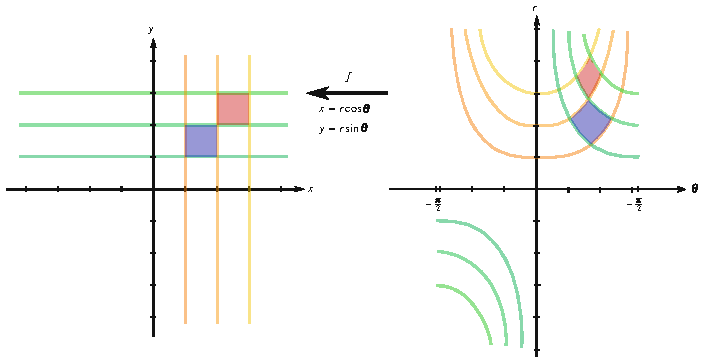
\includegraphics[width=0.960\linewidth]{images/vector/fig-6-10.pdf}
  \caption{映射 $f:\mathbb{R}^2_{r\theta}\to\mathbb{R}^2_{xy}$. 注意阴影区域发生了什么}
  \label{fig:6-10}
\end{figure}

\begin{question}\label{q:6-8}
参考图~\ref{fig:6-10}，用阴影区域解释公式 $T^*f\cdot\bigl(dx\wedge dy\bigr)=-r\,d\theta\wedge dr$.
\end{question}

类似地，我们可以用另一个方向的逆变换
\[
f^{-1}(x,y)=\bigl(r(x,y),\theta(x,y)\bigr)=\left(\pm\sqrt{x^2+y^2},\arctan\frac{y}{x}\right)
\]
来"把面积形式 $d\theta\wedge dr$ 写成 $dx\wedge dy$ 的形式". 首先我们需要求 $d\theta$ 与 $dr$：
\begin{align*}
d\theta&=\frac{\partial\theta}{\partial x}dx+\frac{\partial\theta}{\partial y}dy\\
&=\frac{\partial\arctan(y/x)}{\partial x}dx+\frac{\partial\arctan(y/x)}{\partial y}dy\\
&\overset{\text{链式法则}}{=}\frac{1}{1+(y/x)^2}\frac{\partial}{\partial x}\left(\frac{y}{x}\right)dx
+\frac{1}{1+(y/x)^2}\frac{\partial}{\partial y}\left(\frac{y}{x}\right)dy\\
&=\frac{-y}{x^2+y^2}dx+\frac{x}{x^2+y^2}dy
\end{align*}
以及
\begin{align*}
dr&=\frac{\partial r}{\partial x}dx+\frac{\partial r}{\partial y}dy\\
&=\frac{\partial\bigl(\pm\sqrt{x^2+y^2}\bigr)}{\partial x}dx+\frac{\partial\bigl(\pm\sqrt{x^2+y^2}\bigr)}{\partial y}dy\\
&\overset{\text{链式法则}}{=}\pm\frac{x}{\sqrt{x^2+y^2}}dx\pm\frac{y}{\sqrt{x^2+y^2}}dy
\end{align*}
所以
\begin{align*}
d\theta\wedge dr
&=\left(\frac{-y}{x^2+y^2}dx+\frac{x}{x^2+y^2}dy\right)
\wedge\left(\pm\frac{x}{\sqrt{x^2+y^2}}dx\pm\frac{y}{\sqrt{x^2+y^2}}dy\right)\\
&=\pm\frac{x^2}{(x^2+y^2)\sqrt{x^2+y^2}}dy\wedge dx
-\pm\frac{y^2}{(x^2+y^2)\sqrt{x^2+y^2}}dx\wedge dy\\
&=\pm\frac{-(x^2+y^2)}{(x^2+y^2)\sqrt{x^2+y^2}}dx\wedge dy\\
&=\pm\frac{-1}{\sqrt{x^2+y^2}}dx\wedge dy.
\end{align*}
于是我们得到了恒等式 $d\theta\wedge dr=\frac{-1}{\sqrt{x^2+y^2}}dx\wedge dy$. 和之前一样，我们给定了一个映射 $f^{-1}:\mathbb{R}^2_{xy}\to\mathbb{R}^2_{r\theta}$，它诱导出映射 $Tf^{-1}$ 与 $T^*f^{-1}$，使得
\[
\begin{gathered}
\bigwedge^2\mathbb{R}^2_{xy}\xleftarrow{T^*f^{-1}}\bigwedge^2\mathbb{R}^2_{r\theta}\\
T^*f^{-1}\cdot d\theta\wedge dr\longleftarrow d\theta\wedge dr\\
T\mathbb{R}^2_{xy}\xrightarrow{Tf^{-1}}T\mathbb{R}^2_{r\theta}\\
\mathbb{R}^2_{xy}\xrightarrow{f^{-1}}\mathbb{R}^2_{r\theta}.
\end{gathered}
\]
所以当我们说"把面积形式 $d\theta\wedge dr$ 写成 $dx\wedge dy$ 的形式"时，我们真正的意思是求拉回. 我们得到的恒等式 $d\theta\wedge dr=\frac{-1}{\sqrt{x^2+y^2}}dx\wedge dy$ 实际上应该写成
\[
T^*f^{-1}\cdot\bigl(d\theta\wedge dr\bigr)=\pm\frac{-1}{\sqrt{x^2+y^2}}dx\wedge dy.
\]
由于我们这里实际上处理的是体积形式，我们本可以用另一种方法做所有这些，即利用上一节导出的体积形式拉回的一般公式. 也就是说，给定映射 $\phi:\mathbb{R}^n\to\mathbb{R}^n$，其中
\[
\phi=\bigl(\phi_1(x_1,\ldots,x_n),\phi_2(x_1,\ldots,x_n),\ldots,\phi_n(x_1,\ldots,x_n)\bigr),
\]
体积形式的拉回由下面的等式给出
\[
T^*\phi\cdot\bigl(d\phi_1\wedge d\phi_2\wedge\cdots\wedge d\phi_n\bigr)
=\left|\begin{matrix}
\frac{\partial\phi_1}{\partial x_1}&\frac{\partial\phi_1}{\partial x_2}&\cdots&\frac{\partial\phi_1}{\partial x_n}\\
\frac{\partial\phi_2}{\partial x_1}&\frac{\partial\phi_2}{\partial x_2}&\cdots&\frac{\partial\phi_2}{\partial x_n}\\
\vdots&\vdots&\ddots&\vdots\\
\frac{\partial\phi_n}{\partial x_1}&\frac{\partial\phi_n}{\partial x_2}&\cdots&\frac{\partial\phi_n}{\partial x_n}
\end{matrix}\right|dx_1\wedge dx_2\wedge\cdots\wedge dx_n.
\]
回想一下，体积形式是特殊的. 虽然 Jacobian 矩阵总是给出 $T\phi$，因此总是被用来求向量的前推，但 Jacobian 矩阵只能用来求体积形式的拉回，而不能用来求不是体积形式的其他微分形式的拉回.

首先我们求映射 $f^{-1}(x,y)=\left(\arctan\frac{y}{x},\pm\sqrt{x^2+y^2}\right)$ 的 Jacobian 矩阵为
\[
\begin{bmatrix}
\frac{\partial\theta}{\partial x}&\frac{\partial\theta}{\partial y}\\
\frac{\partial r}{\partial x}&\frac{\partial r}{\partial y}
\end{bmatrix}
=
\begin{bmatrix}
\frac{-y}{x^2+y^2}&\frac{x}{x^2+y^2}\\
\pm\frac{x}{\sqrt{x^2+y^2}}&\pm\frac{y}{\sqrt{x^2+y^2}}
\end{bmatrix}
\]
其行列式为
\[
\left|\begin{matrix}
\frac{-y}{x^2+y^2}&\frac{x}{x^2+y^2}\\
\pm\frac{x}{\sqrt{x^2+y^2}}&\pm\frac{y}{\sqrt{x^2+y^2}}
\end{matrix}\right|
=\pm\frac{-y^2-x^2}{(x^2+y^2)\sqrt{x^2+y^2}}
=\pm\frac{-1}{\sqrt{x^2+y^2}}
\]
这直接给出
\[
T^*f^{-1}\cdot\bigl(d\theta\wedge dr\bigr)=\pm\frac{-1}{\sqrt{x^2+y^2}}dx\wedge dy.
\]
另一个方向也类似地完成：
\[
\left|\begin{matrix}
\frac{\partial x}{\partial\theta}&\frac{\partial x}{\partial r}\\
\frac{\partial y}{\partial\theta}&\frac{\partial y}{\partial r}
\end{matrix}\right|
=
\left|\begin{matrix}
-r\sin\theta&\cos\theta\\
r\cos\theta&\sin\theta
\end{matrix}\right|
=-r\sin^2\theta-r\cos^2\theta=-r
\]
这给出
\[
T^*f\cdot\bigl(dx\wedge dy\bigr)=-r\,d\theta\wedge dr.
\]

现在我们为一个极坐标的例子逐步演算. 通过这个例子和下面的问题，我们将探索笛卡尔坐标与极坐标之间的变换与我们前面几节考察的线性例子相当不同的方式之一. 极坐标变换与线性坐标变换不同的地方在于：两个体积形式之间的关系取决于我们在哪个点. 也就是说，拉回方程取决于基点.

对于由 $f^{-1}(x,y)=\left(\arctan\frac{y}{x},\pm\sqrt{x^2+y^2}\right)$ 给出的极坐标变换 $f^{-1}:\mathbb{R}^2_{xy}\to\mathbb{R}^2_{r\theta}$，我们以弧度给出 $\theta$. 我们的目标是把
\[
(dx\wedge dy)_{(1,1)}\left(\binom{1}{0}_{(1,1)},\binom{0}{1}_{(1,1)}\right)
\]
与
\[
(d\theta\wedge dr)_{f^{-1}(1,1)}\left(T_{(1,1)}f^{-1}\cdot\binom{1}{0}_{(1,1)},T_{(1,1)}f^{-1}\cdot\binom{0}{1}_{(1,1)}\right)
\]
联系起来. 第一个恒等式很简单，我们得到
\[
(dx\wedge dy)_{(1,1)}\left(\binom{1}{0}_{(1,1)},\binom{0}{1}_{(1,1)}\right)
=\left|\begin{matrix}1&0\\0&1\end{matrix}\right|=1.
\]
这里我们用 $xy$ 平面体积形式 $dx\wedge dy$ 求由两个欧几里得单位向量张成的平行六面体的面积. 不出所料，我们得到体积 $1$，正是我们对单位正方形的预期. 现在我们转到下一个恒等式. 首先我们求出 $f^{-1}(1,1)\approx(0.785,1.414)$. 这就是两个欧几里得单位向量的前推的基点. 接下来我们求一般的切映射
\[
T_{(x,y)}f^{-1}
=
\begin{bmatrix}
\frac{\partial\theta}{\partial x}&\frac{\partial\theta}{\partial y}\\
\frac{\partial r}{\partial x}&\frac{\partial r}{\partial y}
\end{bmatrix}
=
\begin{bmatrix}
\frac{-y}{x^2+y^2}&\frac{x}{x^2+y^2}\\
\pm\frac{x}{\sqrt{x^2+y^2}}&\pm\frac{y}{\sqrt{x^2+y^2}}
\end{bmatrix}_{(x,y)}
\]
这意味着对点 $(x,y)=(1,1)$ 我们有
\[
T_{(1,1)}f^{-1}=
\begin{bmatrix}
-\frac12&\frac12\\
\frac{1}{\sqrt{2}}&\frac{1}{\sqrt{2}}
\end{bmatrix}_{(1,1)}.
\]

\begin{figure}[htbp]
  \centering
  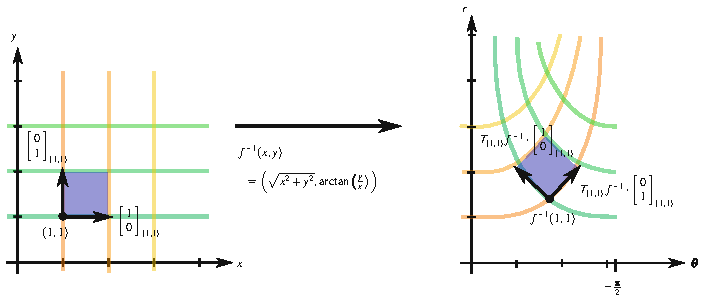
\includegraphics[width=0.960\linewidth]{images/vector/fig-6-11.pdf}
  \caption{在点 $(x,y)=(1,1)$ 与 $f^{-1}(1,1)$ 处体积形式 $dx\wedge dy$ 与 $d\theta\wedge dr$ 之间的关系}
  \label{fig:6-11}
\end{figure}

接下来我们求欧几里得单位向量在 $(1,1)$ 处被 $f^{-1}$ 的前推：
\begin{align*}
T_{(1,1)}f^{-1}\cdot\binom{1}{0}_{(1,1)}
=
\begin{bmatrix}
-\frac12&\frac12\\
\frac{1}{\sqrt{2}}&\frac{1}{\sqrt{2}}
\end{bmatrix}_{(1,1)}
\cdot\binom{1}{0}_{(1,1)}
=
\begin{bmatrix}
-\frac12\\
\frac{1}{\sqrt{2}}
\end{bmatrix}_{(0.785,1.414)}, \\
T_{(1,1)}f^{-1}\cdot\binom{0}{1}_{(1,1)}
=
\begin{bmatrix}
-\frac12&\frac12\\
\frac{1}{\sqrt{2}}&\frac{1}{\sqrt{2}}
\end{bmatrix}_{(1,1)}
\cdot\binom{0}{1}_{(1,1)}
=
\begin{bmatrix}
\frac12\\
\frac{1}{\sqrt{2}}
\end{bmatrix}_{(0.785,1.414)},
\end{align*}
它们被用在
\[
(d\theta\wedge dr)_{(0.785,1.414)}\left(
\begin{bmatrix}
-\frac12\\
\frac{1}{\sqrt{2}}
\end{bmatrix}_{(0.785,1.414)},
\begin{bmatrix}
\frac12\\
\frac{1}{\sqrt{2}}
\end{bmatrix}_{(0.785,1.414)}
\right)
=\left|\begin{matrix}-\frac12&\frac12\\\frac{1}{\sqrt{2}}&\frac{1}{\sqrt{2}}\end{matrix}\right|
=\frac{-1}{\sqrt{2}}.
\]
这里我们用 $r\theta$ 平面体积形式求由被前推的向量张成的平行六面体的体积. 以这种方式算出的面积之间的关系，与在点 $(1,1)\in\mathbb{R}^2_{xy}$ 处由 $T^*f^{-1}\cdot\bigl(d\theta\wedge dr\bigr)=\frac{-1}{\sqrt{x^2+y^2}}dx\wedge dy$ 给出的体积形式 $dx\wedge dy$ 与 $d\theta\wedge dr$ 之间的关系精确对应. 也就是说，
\[
\begin{aligned}
(d\theta\wedge dr)_{f^{-1}(1,1)}&\left(T_{(1,1)}f^{-1}\cdot\binom{1}{0}_{(1,1)},T_{(1,1)}f^{-1}\cdot\binom{0}{1}_{(1,1)}\right)\\
&=\frac{-1}{\sqrt{2}}(dx\wedge dy)_{(1,1)}\left(\binom{1}{0}_{(1,1)},\binom{0}{1}_{(1,1)}\right).
\end{aligned}
\]
换句话说，我们刚刚看到，利用在点 $(1,1)$ 处的两个向量，有
\[
T^*f^{-1}(d\theta\wedge dr)=\frac{-1}{\sqrt{2}}dx\wedge dy.
\]
我们试图在图~\ref{fig:6-11} 中展示正在发生的事情. 现在换一个不同的基点重做最后一个例子，看看会发生什么变化.

\begin{question}\label{q:6-9}
对于由 $f^{-1}(x,y)=\left(\arctan\frac{y}{x},\pm\sqrt{x^2+y^2}\right)$ 给出的极坐标变换 $f^{-1}:\mathbb{R}^2_{xy}\to\mathbb{R}^2_{r\theta}$：
\begin{enumerate}
  \item[(a)] 求 $f^{-1}(2,2)$.
  \item[(b)] 考虑 $\binom{1}{0}_{(2,2)}$ 与 $\binom{0}{1}_{(2,2)}\in T_{(2,2)}\mathbb{R}^2$. 求 $(dx\wedge dy)_{(2,2)}\left(\binom{1}{0}_{(2,2)},\binom{0}{1}_{(2,2)}\right)$.
  \item[(c)] 求 $T_{(2,2)}f^{-1}$.
  \item[(d)] 求 $T_{(2,2)}f^{-1}\cdot\binom{1}{0}_{(2,2)}$ 与 $T_{(2,2)}f^{-1}\cdot\binom{0}{1}_{(2,2)}$. （这些是欧几里得单位向量在 $(2,2)$ 处被 $f^{-1}$ 前推到 $f^{-1}(2,2)$ 的结果.）
  \item[(e)] 求 $(d\theta\wedge dr)_{f^{-1}(2,2)}\left(T_{(2,2)}f^{-1}\cdot\binom{1}{0}_{(2,2)},T_{(2,2)}f^{-1}\cdot\binom{0}{1}_{(2,2)}\right)$.
\end{enumerate}
\end{question}

图~\ref{fig:6-12} 展示了这道题中发生的事情. 你在这道题中应该得到的关系是
\[
\begin{aligned}
(d\theta\wedge dr)_{f^{-1}(2,2)}&\left(T_{(2,2)}f^{-1}\cdot\binom{1}{0}_{(2,2)},T_{(2,2)}f^{-1}\cdot\binom{0}{1}_{(2,2)}\right)\\
&=\frac{-1}{\sqrt{8}}(dx\wedge dy)_{(2,2)}\left(\binom{1}{0}_{(2,2)},\binom{0}{1}_{(2,2)}\right).
\end{aligned}
\]
数值系数发生了变化. 这是因为我们求面积的基点发生了变化. 换句话说，$xy$ 平面与 $r\theta$ 平面中面积形式之间的关系取决于面积形式被使用的点. 所以，在点 $(1,1)$ 处我们有
\[
T_{(1,1)}^*f^{-1}\cdot\bigl(d\theta\wedge dr\bigr)=\frac{-1}{\sqrt{2}}dx\wedge dy
\]
而在点 $(2,2)$ 处我们有
\[
T_{(2,2)}^*f^{-1}\cdot\bigl(d\theta\wedge dr\bigr)=\frac{-1}{\sqrt{8}}dx\wedge dy
\]
这正是我们从前面的实际恒等式所预期的：
\[
T_{(x,y)}^*f^{-1}\cdot\bigl(d\theta\wedge dr\bigr)=\pm\frac{-1}{\sqrt{x^2+y^2}}dx\wedge dy.
\]

\begin{figure}[htbp]
  \centering
  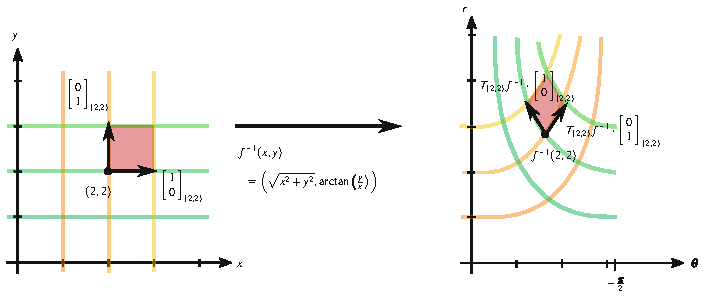
\includegraphics[width=0.960\linewidth]{images/vector/fig-6-12.pdf}
  \caption{在点 $(x,y)=(2,2)$ 与 $f^{-1}(2,2)$ 处体积形式 $dx\wedge dy$ 与 $d\theta\wedge dr$ 之间的关系}
  \label{fig:6-12}
\end{figure}

\section{柱坐标与球坐标}

柱坐标与球坐标是 $\mathbb{R}^3$ 非常常用的两个坐标系. 既然我们现在对向量的前推与体积形式的拉回有了相当好的认识，我们将在本节提供较少的细节. 柱坐标变换 $f:\mathbb{R}^3_{r\theta z}\to\mathbb{R}^3_{xyz}$ 由
\[
f(r,\theta,z)=\bigl(x(r,\theta,z),y(r,\theta,z),z(r,\theta,z)\bigr)=\bigl(r\cos\theta,r\sin\theta,z\bigr)
\]
给出，在微积分课上它一般写成
\[
x=r\cos\theta,\qquad y=r\sin\theta,\qquad z=z.
\]
见图~\ref{fig:6-13}. 柱坐标变换 $f$ 诱导出如下映射：
\[
\begin{gathered}
\bigwedge^3\mathbb{R}^3_{r\theta z}\xleftarrow{T^*f}\bigwedge^3\mathbb{R}^3_{xyz}\\
T_{(r,\theta,z)}^*f\cdot\bigl(dx\wedge dy\wedge dz\bigr)\longleftarrow dx\wedge dy\wedge dz\\
\mathbb{R}^3_{r\theta z}\xrightarrow{Tf}\mathbb{R}^3_{xyz}\\
v_{(r,\theta,z)}\longmapsto T_{(r,\theta,z)}f\cdot v_{(r,\theta,z)}\\
\mathbb{R}^3_{r\theta z}\xrightarrow{f}\mathbb{R}^3_{xyz}\\
(r,\theta,z)\longmapsto\bigl(r\cos\theta,r\sin\theta,z\bigr).
\end{gathered}
\]

\begin{figure}[htbp]
  \centering
  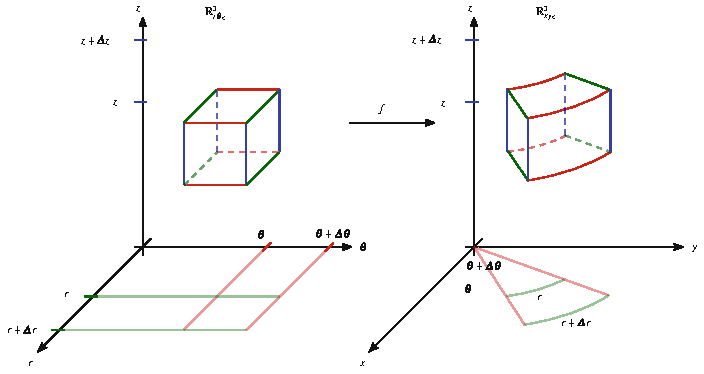
\includegraphics[width=0.960\linewidth]{images/vector/fig-6-13.pdf}
  \caption{由 $x=r\cos\theta$、$y=r\sin\theta$、$z=z$ 给出的柱坐标映射 $f:\mathbb{R}^3_{r\theta z}\to\mathbb{R}^3_{xyz}$. $\mathbb{R}^3_{r\theta z}$ 中的立方体被映射为 $\mathbb{R}^3_{xyz}$ 中的楔形体}
  \label{fig:6-13}
\end{figure}

和之前一样进行，要么利用楔积的性质，要么利用以 Jacobian 形式给出的楔积公式，我们可以把 $dx\wedge dy\wedge dz$ 写成 $d\theta\wedge dr\wedge dz$ 的形式. 这里我们求
\begin{align*}
dx=\frac{\partial x}{\partial\theta}d\theta+\frac{\partial x}{\partial r}dr+\frac{\partial x}{\partial z}dz=-r\sin\theta\,d\theta+\cos\theta\,dr, \\
dy=\frac{\partial y}{\partial\theta}d\theta+\frac{\partial y}{\partial r}dr+\frac{\partial y}{\partial z}dz=r\cos\theta\,d\theta+\sin\theta\,dr, \\
dz=\frac{\partial z}{\partial\theta}d\theta+\frac{\partial z}{\partial r}dr+\frac{\partial z}{\partial z}dz=dz
\end{align*}
我们用它来得到
\begin{align*}
dx\wedge dy\wedge dz&=\bigl(-r\sin\theta\,d\theta+\cos\theta\,dr\bigr)\wedge\bigl(r\cos\theta\,d\theta+\sin\theta\,dr\bigr)\wedge dz\\
&=\bigl(-r\sin^2\theta\,d\theta\wedge dr+r\cos^2\theta\,dr\wedge d\theta\bigr)\wedge dz\\
&=-r\,d\theta\wedge dr\wedge dz.
\end{align*}
正如我们现在所知，这个恒等式的真正含义是
\[
T_{(r,\theta,z)}^*f\cdot\bigl(dx\wedge dy\wedge dz\bigr)=-r\,d\theta\wedge dr\wedge dz.
\]
我们刚才所做的正是求微积分中通常给出的"$\theta rz$ 体积元". 很多微积分书给出一个看起来像图~\ref{fig:6-14} 的"$\theta rz$ 体积元"图画，然后用这幅图来求体积变化公式，尽管定向没有被考虑进去. 因此，即使我们的处理方式比你见过的任何微积分都抽象和理论化得多，你对它也已经从另一个视角熟悉了.

\begin{figure}[htbp]
  \centering
  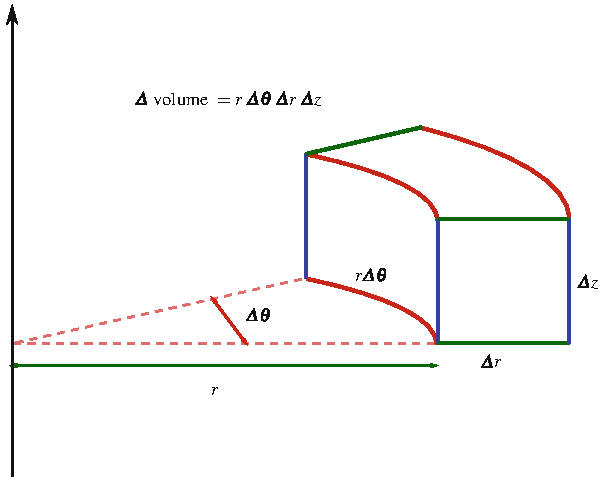
\includegraphics[width=0.717\linewidth]{images/vector/fig-6-14.pdf}
  \caption{大多数微积分教科书中给出的柱坐标"$\theta rz$ 体积元"}
  \label{fig:6-14}
\end{figure}

\begin{question}\label{q:6-10}
利用体积形式拉回的公式求 $T_{(r,\theta,z)}^*f\cdot\bigl(dx\wedge dy\wedge dz\bigr)$.
\end{question}

\begin{question}\label{q:6-11}
解释公式 $T_{(r,\theta,z)}^*f\cdot\bigl(dx\wedge dy\wedge dz\bigr)=-r\,d\theta\wedge dr\wedge dz$ 与图~\ref{fig:6-14} 所示"$\theta rz$ 体积元"之间的关系.
\end{question}

现在我们转向球坐标变换. 球坐标变换 $g:\mathbb{R}^3_{\rho\varphi\theta}\to\mathbb{R}^3_{xyz}$ 由
\[
g(\rho,\varphi,\theta)=\bigl(x(\rho,\varphi,\theta),y(\rho,\varphi,\theta),z(\rho,\varphi,\theta)\bigr)
=\bigl(\rho\sin\varphi\cos\theta,\rho\sin\varphi\sin\theta,\rho\cos\varphi\bigr)
\]
给出，在微积分课上它一般写成
\[
x=\rho\sin\varphi\cos\theta,\qquad y=\rho\sin\varphi\sin\theta,\qquad z=\rho\cos\varphi.
\]
映射 $g:\mathbb{R}^3_{\rho\varphi\theta}\to\mathbb{R}^3_{xyz}$ 在图~\ref{fig:6-15} 中作了说明. 球坐标变换诱导出如下映射：
\[
\begin{gathered}
\bigwedge^3\mathbb{R}^3_{\rho\varphi\theta}\xleftarrow{T^*g}\bigwedge^3\mathbb{R}^3_{xyz}\\
T_{(\rho,\varphi,\theta)}^*g\cdot\bigl(dx\wedge dy\wedge dz\bigr)\longleftarrow dx\wedge dy\wedge dz\\
\mathbb{R}^3_{\rho\varphi\theta}\xrightarrow{Tg}\mathbb{R}^3_{xyz}\\
v_{(\rho,\varphi,\theta)}\longmapsto T_{(\rho,\varphi,\theta)}g\cdot v_{(\rho,\varphi,\theta)}\\
\mathbb{R}^3_{\rho\varphi\theta}\xrightarrow{g}\mathbb{R}^3_{xyz}\\
(\rho,\varphi,\theta)\longmapsto\bigl(\rho\sin\varphi\cos\theta,\rho\sin\varphi\sin\theta,\rho\cos\varphi\bigr).
\end{gathered}
\]

\begin{figure}[htbp]
  \centering
  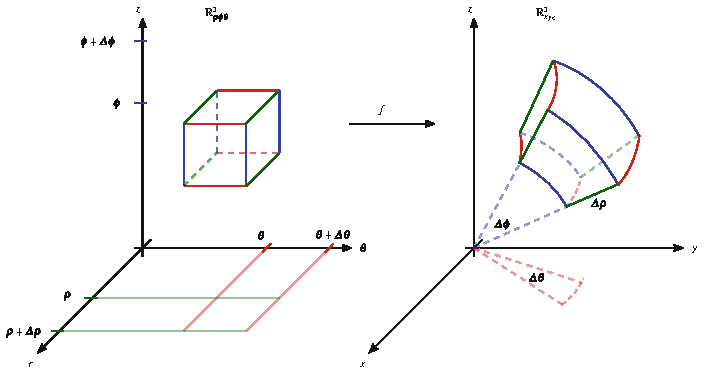
\includegraphics[width=0.960\linewidth]{images/vector/fig-6-15.pdf}
  \caption{由 $x=\rho\sin\varphi\cos\theta$、$y=\rho\sin\varphi\sin\theta$、$z=\rho\cos\varphi$ 给出的球坐标变换 $g:\mathbb{R}^3_{\rho\varphi\theta}\to\mathbb{R}^3_{xyz}$}
  \label{fig:6-15}
\end{figure}

同样，一个直截了当的计算表明
\begin{align*}
dx=\sin\varphi\cos\theta\,d\rho-\rho\sin\varphi\sin\theta\,d\theta+\rho\cos\varphi\cos\theta\,d\varphi, \\
dy=\sin\varphi\sin\theta\,d\rho+\rho\sin\varphi\cos\theta\,d\theta+\rho\cos\varphi\sin\theta\,d\varphi, \\
dz=\cos\varphi\,d\rho-\rho\sin\varphi\,d\varphi.
\end{align*}
另一个直截了当但稍长一些、应该由你自己完成的计算给出
\[
dx\wedge dy\wedge dz=-\rho^2\sin\varphi\,d\rho\wedge d\theta\wedge d\varphi.
\]
正如我们现在所知道的，这个恒等式的真正含义是
\[
T_{(\rho,\varphi,\theta)}^*g\cdot\bigl(dx\wedge dy\wedge dz\bigr)=-\rho^2\sin\varphi\,d\rho\wedge d\theta\wedge d\varphi.
\]
由于 $dx\wedge dy\wedge dz$ 是体积形式，我们本可以用体积形式拉回的公式求出它. 很多微积分书给出一个看起来像图~\ref{fig:6-16} 的"$\rho\varphi\theta$ 体积元"图画. 注意我们如何能从这幅图图解地看出体积的变化，尽管定向仍然没有被考虑进去. 所以同样，尽管我们从更抽象的角度来讨论这一点，但这是你在微积分中已经接触过的东西.

\begin{figure}[htbp]
  \centering
  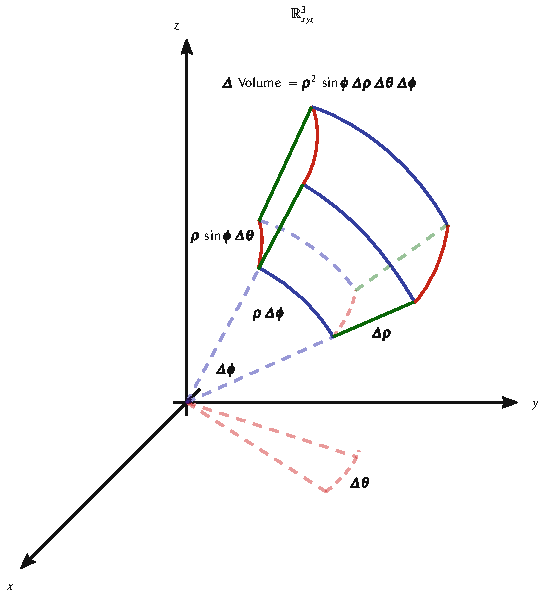
\includegraphics[width=0.715\linewidth]{images/vector/fig-6-16.pdf}
  \caption{大多数微积分教科书中给出的球坐标"$\rho\varphi\theta$ 体积元"}
  \label{fig:6-16}
\end{figure}

\begin{question}\label{q:6-12}
利用体积形式拉回的公式求 $T_{(\rho,\varphi,\theta)}^*g\cdot\bigl(dx\wedge dy\wedge dz\bigr)$.
\end{question}

\begin{question}\label{q:6-13}
解释公式 $T_{(\rho,\varphi,\theta)}^*g\cdot\bigl(dx\wedge dy\wedge dz\bigr)=-\rho^2\sin\varphi\,d\rho\wedge d\theta\wedge d\varphi$ 与图~\ref{fig:6-16} 所示"$\rho\varphi\theta$ 体积元"之间的关系.
\end{question}

\section{微分形式的拉回}

考虑我们在前几节得到的若干关系
\begin{align*}
T^*f\cdot(dx\wedge dy)=-\frac12du\wedge dv\qquad\text{(线性例子)} \\
T^*f\cdot(dx\wedge dy)=-r\,d\theta\wedge dr\qquad\text{(极坐标)} \\
T^*f\cdot(dx\wedge dy\wedge dz)=-r\,d\theta\wedge dr\wedge dz\qquad\text{(柱坐标)} \\
T^*f\cdot(dx\wedge dy\wedge dz)=-\rho^2\sin\varphi\,d\rho\wedge d\theta\wedge d\varphi\qquad\text{(球坐标)}
\end{align*}
其中 $f$ 是相应的映射 $f:\mathbb{R}^{n}_{\text{其他坐标}}\to\mathbb{R}^{n}_{\text{欧几里得}}$. 根据我们给出的体积形式拉回的定义，这些式子真正意味着
\begin{align*}
\underbrace{-\frac12(du\wedge dv)_p(v_p,w_p)}_{=\ T_p^*f\cdot(dx\wedge dy)_{f(p)}}=(dx\wedge dy)_{f(p)}(T_pf\cdot v_p,T_pf\cdot w_p), \\
\underbrace{-r(d\theta\wedge dr)_p(v_p,w_p)}_{=\ T_p^*f\cdot(dx\wedge dy)_{f(p)}}=(dx\wedge dy)_{f(p)}(T_pf\cdot v_p,T_pf\cdot w_p), \\
\underbrace{-r(d\theta\wedge dr\wedge dz)_p(u_p,v_p,w_p)}_{=\ T_p^*f\cdot(dx\wedge dy\wedge dz)_{f(p)}}=(dx\wedge dy\wedge dz)_{f(p)}(T_pf\cdot u_p,T_pf\cdot v_p,T_pf\cdot w_p), \\
\underbrace{-\rho^2\sin\varphi(d\rho\wedge d\theta\wedge d\varphi)_p(u_p,v_p,w_p)}_{=\ T_p^*f\cdot(dx\wedge dy\wedge dz)_{f(p)}}=(dx\wedge dy\wedge dz)_{f(p)}(T_pf\cdot u_p,T_pf\cdot v_p,T_pf\cdot w_p).
\end{align*}

现在我们花一点时间再详细地给出微分形式拉回的定义. 假设我们有映射 $\varphi:\mathbb{R}^n\to\mathbb{R}^m$，其中
\[
\varphi(x_1,x_2,\ldots,x_n)=\bigl(\varphi_1(x_1,x_2,\ldots,x_n),\varphi_2(x_1,x_2,\ldots,x_n),\ldots,\varphi_m(x_1,x_2,\ldots,x_n)\bigr).
\]
$\varphi$ 定义一个映射，称为 $\varphi$ 的前推或切映射，记为 $T\varphi:T\mathbb{R}^n\to T\mathbb{R}^m$，它从 $\mathbb{R}^n$ 的切丛到 $\mathbb{R}^m$ 的切丛. 在坐标下，映射 $T\varphi$ 由 Jacobian 矩阵给出：
\[
T\varphi=
\begin{bmatrix}
\frac{\partial\varphi_1}{\partial x_1}&\cdots&\frac{\partial\varphi_1}{\partial x_n}\\
\vdots&\ddots&\vdots\\
\frac{\partial\varphi_m}{\partial x_1}&\cdots&\frac{\partial\varphi_m}{\partial x_n}
\end{bmatrix}.
\]
正如已经提到过的，人们经常遇到的 $T\varphi$ 的其他记号是 $D\varphi$ 与 $\varphi_*$. 我们用这个前推映射 $T\varphi$ 来帮助定义另一个映射，称为微分形式被 $\varphi$ 的拉回，或简称为被 $\varphi$ 的拉回，记为 $T^*\varphi$ 或 $\varphi^*$. 实际上，$\varphi^*$ 是拉回的标准记号，但我们将使用 $T^*\varphi$.

在真正定义 $T^*\varphi$ 之前，我们要说明它作用于哪些空间. 回想记号 $\bigwedge^k\mathbb{R}^n$ 用来表示 $\mathbb{R}^n$ 上 $k$-形式的向量空间，而
\[
\bigwedge\mathbb{R}^n=\bigcup_{k=1}^{\infty}\bigwedge^k\mathbb{R}^n
\]
表示 $\mathbb{R}^n$ 上任意大小的所有微分形式的集合. 利用这一点，我们一般把映射 $\varphi$ 及其诱导映射 $T\varphi$ 与 $T^*\varphi$ 画成
\[
\begin{gathered}
\bigwedge\mathbb{R}^n\xleftarrow{T^*\varphi}\bigwedge\mathbb{R}^m\\
T\mathbb{R}^n\xrightarrow{T\varphi}T\mathbb{R}^m\\
\mathbb{R}^n\xrightarrow{\varphi}\mathbb{R}^m.
\end{gathered}
\]
所以，拉回映射作用于空间 $\bigwedge\mathbb{R}^m$，它取 $\mathbb{R}^m$ 上的一个微分形式，产生 $\bigwedge\mathbb{R}^n$ 的一个元素，即 $\mathbb{R}^n$ 上的一个微分形式. 注意这个映射的方向与 $\varphi$ 和 $T\varphi$ 相反. 这就是为什么 $T^*\varphi$ 被称为拉回而 $T\varphi$ 被称为前推. 接下来，即使 $T^*\varphi$ 作用于任意阶的 $k$-形式，我们有时也滥用记号写成
\[
T^*\mathbb{R}^n\xleftarrow{T^*\varphi}T^*\mathbb{R}^m,
\]
即用 $T^*\mathbb{R}^n$ 与 $T^*\mathbb{R}^m$ 代替 $\bigwedge\mathbb{R}^n$ 与 $\bigwedge\mathbb{R}^m$. 我们把 $k$-形式 $\alpha$ 的拉回，即 $T^*\varphi\cdot\alpha\in\bigwedge^k\mathbb{R}^n$，定义为 $\alpha\in\bigwedge^k\mathbb{R}^m$ 作用于被前推的向量 $T\varphi\cdot v_i\in T\mathbb{R}^m$：

\begin{definition}[$\alpha$ 的拉回]\label{def:6-6-1}
\[
\bigl(T^*\varphi\cdot\alpha\bigr)(v_1,v_2,\ldots,v_k)\equiv\alpha\bigl(T\varphi\cdot v_1,T\varphi\cdot v_2,\ldots,T\varphi\cdot v_k\bigr).
\]
\end{definition}

如果我们想小心一点并开始跟踪基点，记号就开始变得有点笨拙了，尽管有时你确实需要这样做. 这个记号的一个奇怪之处是，映射 $T^*\varphi$ 不是按它来自的点加下标，而是按它去往的点加下标. 这样做是为了使拉回与前推映射 $T_p^*\varphi$ 与 $T_p\varphi$ 的记号保持一致，也就是说，使它们彼此"对偶". 这种事情并不常发生，而且你头几次看到它时肯定会觉得奇怪.
\[
\begin{gathered}
\mathbb{R}^n_p\xleftarrow{T_p^*\varphi}\mathbb{R}^m_{\varphi(p)}\\
T_p\mathbb{R}^n\xrightarrow{T_p\varphi}T_{\varphi(p)}\mathbb{R}^m\\
\mathbb{R}^n\xrightarrow{\varphi}\mathbb{R}^m.
\end{gathered}
\]
加上基点之后，我们有以下定义
\[
\underbrace{\bigl(T_p^*\varphi\cdot\alpha_{\varphi(p)}\bigr)\bigl(v_{1_p},v_{2_p},\ldots,v_{k_p}\bigr)}_{\text{$\alpha$ 的拉回}}\equiv\alpha_{\varphi(p)}\bigl(T_p\varphi\cdot v_{1_p},T_p\varphi\cdot v_{2_p},\ldots,T_p\varphi\cdot v_{k_p}\bigr).
\]

现在，为了实际看到这是如何工作的，让我们考虑几个例子. 我们已经大量研究了体积形式，所以现在我们转向任意 $k$ 的 $k$-形式. 遗憾的是没有求任意形式拉回的好公式，但有一个相当标准的步骤可以使用. 考虑由 $\varphi(x,y)=(x+y,x-y)$ 给出的映射 $\varphi:\mathbb{R}^2_{xy}\to\mathbb{R}^2_{uv}$ 以及 $\mathbb{R}^2_{uv}$ 上的 1-形式 $\alpha=vdu+udv$. 我们想在 $\mathbb{R}^2_{xy}$ 上求 $T^*\varphi\cdot\alpha$. 注意，我们现在处理的是一个 1-形式，而不是体积形式.

我们将按如下方式处理这个问题. $\alpha$ 的拉回 $T^*\varphi\cdot\alpha$ 将是 $\mathbb{R}^2_{xy}$ 上的一个 1-形式，因此它将具有 $f(x,y)dx+g(x,y)dy$ 的形式，其中 $f$ 与 $g$ 是迄今未知的函数. 正是这些函数是我们想求的. 首先我们注意到
\[
(fdx+gdy)\binom{1}{0}=f\,dx\binom{1}{0}+g\,dy\binom{1}{0}=f(1)+g(0)=f
\]
以及
\[
(fdx+gdy)\binom{0}{1}=f\,dx\binom{0}{1}+g\,dy\binom{0}{1}=f(0)+g(1)=g.
\]
我们将用这些恒等式求出 $f$ 和 $g$ 是什么. 我们还需要恒等式
\[
T\varphi=
\begin{bmatrix}
1&1\\
1&-1
\end{bmatrix}.
\]
我们现在继续用上面的恒等式求 $f$ 与 $g$，如下所示：
\begin{align*}
f&=(fdx+gdy)\binom{1}{0}=(T^*\varphi\cdot\alpha)\binom{1}{0}\\
&=\alpha\left(T\varphi\cdot\binom{1}{0}\right)=(vdu+udv)\left(\begin{bmatrix}1&1\\1&-1\end{bmatrix}\cdot\binom{1}{0}\right)\\
&=(vdu+udv)\binom{1}{1}=v\,du\binom{1}{1}+u\,dv\binom{1}{1}\\
&=u+v=(x+y)+(x-y)=2x
\end{align*}
以及
\begin{align*}
g&=(fdx+gdy)\binom{0}{1}=(T^*\varphi\cdot\alpha)\binom{0}{1}\\
&=\alpha\left(T\varphi\cdot\binom{0}{1}\right)=(vdu+udv)\left(\begin{bmatrix}1&1\\1&-1\end{bmatrix}\cdot\binom{0}{1}\right)\\
&=(vdu+udv)\binom{1}{-1}=v\,du\binom{1}{-1}+u\,dv\binom{1}{-1}\\
&=u-v=(x+y)-(x-y)=2y.
\end{align*}
把一切结合起来，我们有
\[
T^*\varphi\cdot\bigl(vdu+udv\bigr)=2x\,dx+2y\,dy.
\]
注意在这个例子中我们是怎样求出 $T^*\varphi\cdot\alpha$ 的精确形式的. 知道拉回是一个 1-形式意味着我们知道它必须是函数乘以基元素 $dx$ 与 $dy$ 的和. 我们还知道 $dx\binom{1}{0}=1$ 与 $dy\binom{0}{1}=1$，所以我们可以用这些向量的前推求出所需的函数.

现在考虑同一个映射 $\varphi:\mathbb{R}^2_{xy}\to\mathbb{R}^2_{uv}$，其中 $\varphi(x,y)=(x+y,x-y)$，以及 2-形式 $\alpha=du\wedge dv$. 我们想求 $T^*\varphi\cdot\alpha$. 我猜你会注意到我们又回到了面积形式，所以你对我们得到的答案不会感到惊讶——我们只是用不同的方式得到它而已. 显然 $T^*\varphi\cdot\alpha$ 将是 $\mathbb{R}^2_{xy}$ 上的一个 2-形式，所以它将具有 $f(x,y)dx\wedge dy$ 的形式，其中 $f$ 是某个函数，因为 $dx\wedge dy$ 是 $\mathbb{R}^2$ 上 2-形式的唯一基元素. 接下来我们问自己，哪两个向量被 $dx\wedge dy$"吃进"后给出 $1$？显然 $\binom{1}{0}$ 与 $\binom{0}{1}$ 可以，因为
\[
dx\wedge dy\left(\binom{1}{0},\binom{0}{1}\right)=\left|\begin{matrix}1&0\\0&1\end{matrix}\right|=1.
\]
利用这一点我们有
\begin{align*}
f&=f\,dx\wedge dy\left(\binom{1}{0},\binom{0}{1}\right)\\
&=(T^*\varphi\cdot\alpha)\left(\binom{1}{0},\binom{0}{1}\right)\\
&=\alpha\left(T\varphi\cdot\binom{1}{0},T\varphi\cdot\binom{0}{1}\right)\\
&=du\wedge dv\left(\begin{bmatrix}1&1\\1&-1\end{bmatrix}\cdot\binom{1}{0},\begin{bmatrix}1&1\\1&-1\end{bmatrix}\cdot\binom{0}{1}\right)\\
&=du\wedge dv\left(\binom{1}{1},\binom{1}{-1}\right)\\
&=\left|\begin{matrix}1&1\\1&-1\end{matrix}\right|\\
&=-2.
\end{align*}
把一切放在一起我们得到
\[
-2dx\wedge dy=T^*\varphi\cdot\bigl(du\wedge dv\bigr).
\]

\begin{question}\label{q:6-14}
现在考虑由 $\varphi^{-1}(u,v)=\left(\frac12(u+v),\frac12(u-v)\right)$ 给出的逆映射 $\varphi^{-1}:\mathbb{R}^2_{uv}\to\mathbb{R}^2_{xy}$，并设 $\alpha=dx\wedge dy$. 用这种方法求 $T^*\varphi^{-1}\cdot\alpha$.
\end{question}

现在我们再考虑几个复杂性渐增的例子. 假设 $\varphi:\mathbb{R}^2_{xy}\to\mathbb{R}^3_{uvw}$ 由 $f(x,y)=\bigl(u(x,y),v(x,y),w(x,y)\bigr)=(x+y,x-y,xy)$ 给出，并考虑 $\mathbb{R}^3$ 上的 1-形式 $\alpha=vdu+wdv+udw$. 我们想求 $T^*\varphi\cdot\alpha$. 和之前一样，$T^*\varphi\cdot\alpha$ 将具有 $fdx+gdy$ 的形式，其中 $f$ 与 $g$ 是某些函数，所以和之前一样我们将用向量 $\binom{1}{0}$ 与 $\binom{0}{1}$. 另外，
\[
T\varphi=
\begin{bmatrix}
\frac{\partial u}{\partial x}&\frac{\partial u}{\partial y}\\
\frac{\partial v}{\partial x}&\frac{\partial v}{\partial y}\\
\frac{\partial w}{\partial x}&\frac{\partial w}{\partial y}
\end{bmatrix}
=
\begin{bmatrix}
1&1\\
1&-1\\
y&x
\end{bmatrix}
\]
所以
\begin{align*}
f&=(fdx+gdy)\binom{1}{0}\\
&=(T^*\varphi\cdot\alpha)\binom{1}{0}\\
&=\alpha\left(T\varphi\cdot\binom{1}{0}\right)\\
&=(vdu+wdv+udw)\left(\begin{bmatrix}1&1\\1&-1\\y&x\end{bmatrix}\cdot\binom{1}{0}\right)\\
&=(vdu+wdv+udw)\begin{bmatrix}1\\1\\y\end{bmatrix}\\
&=v(1)+w(1)+u(y)\\
&=(x-y)(1)+(xy)(1)+(x+y)(y)\\
&=x-y+2xy+y^2
\end{align*}
以及
\begin{align*}
g&=(fdx+gdy)\binom{0}{1}\\
&=(T^*\varphi\cdot\alpha)\binom{0}{1}\\
&=\alpha\left(T\varphi\cdot\binom{0}{1}\right)\\
&=(vdu+wdv+udw)\left(\begin{bmatrix}1&1\\1&-1\\y&x\end{bmatrix}\cdot\binom{0}{1}\right)\\
&=(vdu+wdv+udw)\begin{bmatrix}1\\-1\\x\end{bmatrix}\\
&=v(1)+w(-1)+u(x)\\
&=(x-y)(1)+(xy)(-1)+(x+y)(x)\\
&=x-y+x^2
\end{align*}
所以我们有
\[
T^*\varphi\cdot\bigl(vdu+wdv+udw\bigr)=\bigl(x-y+2xy+y^2\bigr)dx+\bigl(x-y+x^2\bigr)dy.
\]

接下来假设我们有映射 $\varphi:\mathbb{R}^3_{abc}\to\mathbb{R}^4_{xyzw}$，其中
\[
\varphi(a,b,c)=\bigl(x(a,b,c),y(a,b,c),z(a,b,c),w(a,b,c)\bigr)=(a,b,c,abc).
\]
如果 $\omega=x^2dy\wedge dz+y^2dz\wedge dw$ 是 $\mathbb{R}^4$ 上的一个 2-形式，求 $T^*\varphi\cdot\omega$. 首先我们求前推映射
\[
T\varphi=
\begin{bmatrix}
\frac{\partial x}{\partial a}&\frac{\partial x}{\partial b}&\frac{\partial x}{\partial c}\\
\frac{\partial y}{\partial a}&\frac{\partial y}{\partial b}&\frac{\partial y}{\partial c}\\
\frac{\partial z}{\partial a}&\frac{\partial z}{\partial b}&\frac{\partial z}{\partial c}\\
\frac{\partial w}{\partial a}&\frac{\partial w}{\partial b}&\frac{\partial w}{\partial c}
\end{bmatrix}
=
\begin{bmatrix}
1&0&0\\
0&1&0\\
0&0&1\\
bc&ac&ab
\end{bmatrix}
\]
以及 $\mathbb{R}^3$ 基向量的前推：
\[
T\varphi\cdot\begin{bmatrix}1\\0\\0\end{bmatrix}
=
\begin{bmatrix}1\\0\\0\\bc\end{bmatrix},\qquad
T\varphi\cdot\begin{bmatrix}0\\1\\0\end{bmatrix}
=
\begin{bmatrix}0\\1\\0\\ac\end{bmatrix},\qquad
T\varphi\cdot\begin{bmatrix}0\\0\\1\end{bmatrix}
=
\begin{bmatrix}0\\0\\1\\ab\end{bmatrix}.
\]
我们知道 $\mathbb{R}^3$ 上的所有 2-形式都在 $\mathrm{span}\{da\wedge db,db\wedge dc,dc\wedge da\}$ 中，所以
\[
T^*\varphi\cdot\omega=f\,da\wedge db+g\,db\wedge dc+h\,dc\wedge da
\]
其中 $f,g,h$ 是某些函数. 另外，我们知道
\begin{align*}
da\wedge db\left(\begin{bmatrix}1\\0\\0\end{bmatrix},\begin{bmatrix}0\\1\\0\end{bmatrix}\right)
=\left|\begin{matrix}1&0\\0&1\end{matrix}\right|=1, \\
db\wedge dc\left(\begin{bmatrix}0\\1\\0\end{bmatrix},\begin{bmatrix}0\\0\\1\end{bmatrix}\right)
=\left|\begin{matrix}1&0\\0&1\end{matrix}\right|=1, \\
dc\wedge da\left(\begin{bmatrix}0\\0\\1\end{bmatrix},\begin{bmatrix}1\\0\\0\end{bmatrix}\right)
=\left|\begin{matrix}1&0\\0&1\end{matrix}\right|=1.
\end{align*}
基 2-形式与向量的所有其他组合都等于零. 与之前相同的策略，我们有
\begin{align*}
f&=\bigl(f\,da\wedge db+g\,db\wedge dc+h\,dc\wedge da\bigr)\left(\begin{bmatrix}1\\0\\0\end{bmatrix},\begin{bmatrix}0\\1\\0\end{bmatrix}\right)\\
&=(T^*\varphi\cdot\omega)\left(\begin{bmatrix}1\\0\\0\end{bmatrix},\begin{bmatrix}0\\1\\0\end{bmatrix}\right)\\
&=\left(x^2dy\wedge dz+y^2dz\wedge dw\right)\left(T\varphi\cdot\begin{bmatrix}1\\0\\0\end{bmatrix},T\varphi\cdot\begin{bmatrix}0\\1\\0\end{bmatrix}\right)\\
&=\left(x^2dy\wedge dz+y^2dz\wedge dw\right)\left(\begin{bmatrix}1\\0\\0\\bc\end{bmatrix},\begin{bmatrix}0\\1\\0\\ac\end{bmatrix}\right)\\
&=x^2dy\wedge dz\left(\begin{bmatrix}1\\0\\0\\bc\end{bmatrix},\begin{bmatrix}0\\1\\0\\ac\end{bmatrix}\right)
+y^2dz\wedge dw\left(\begin{bmatrix}1\\0\\0\\bc\end{bmatrix},\begin{bmatrix}0\\1\\0\\ac\end{bmatrix}\right)\\
&=x^2\left|\begin{matrix}0&1\\0&0\end{matrix}\right|
+y^2\left|\begin{matrix}0&0\\bc&ac\end{matrix}\right|\\
&=0.
\end{align*}
类似地我们有
\begin{align*}
g&=\ldots=x^2\left|\begin{matrix}1&0\\0&1\end{matrix}\right|
+y^2\left|\begin{matrix}0&1\\ac&ab\end{matrix}\right|\\
&=x^2(1)+y^2(-ac)\\
&=a^2-ab^2c
\end{align*}
以及
\begin{align*}
h&=\ldots=x^2\left|\begin{matrix}0&0\\1&0\end{matrix}\right|
+y^2\left|\begin{matrix}1&0\\ab&bc\end{matrix}\right|\\
&=x^2(0)+y^2(bc)\\
&=b^3c.
\end{align*}
因此
\[
T^*\varphi\cdot\bigl(x^2dy\wedge dz+y^2dz\wedge dw\bigr)=\bigl(a^2-ab^2c\bigr)db\wedge dc+\bigl(b^3c\bigr)dc\wedge da.
\]

\begin{question}\label{q:6-15}
把上面两个计算中的 $\ldots$ 补全.
\end{question}

\begin{question}\label{q:6-16}
同一个映射下 $dx\wedge dy\wedge dz\wedge dw$ 的拉回是什么？
\end{question}

\begin{question}\label{q:6-17}
假设我们有映射 $\varphi:\mathbb{R}^n_{x_1\cdots x_n}\to\mathbb{R}^m_{\varphi_1\cdots\varphi_m}$，其中 $m>n$，$\varphi=(\varphi_1,\ldots,\varphi_m)$，且 $\omega$ 是 $\mathbb{R}^m$ 上的一个 $n$-形式. 证明
\[
T_p^*\varphi\cdot\omega=\omega_{\varphi(p)}\left(\frac{\partial\varphi}{\partial x_1},\ldots,\frac{\partial\varphi}{\partial x_n}\right)dx_1\wedge dx_2\wedge\cdots\wedge dx_n
\]
其中
\[
\frac{\partial\varphi}{\partial x_i}=
\begin{bmatrix}
\frac{\partial\varphi_1}{\partial x_i}\\
\frac{\partial\varphi_2}{\partial x_i}\\
\vdots\\
\frac{\partial\varphi_m}{\partial x_i}
\end{bmatrix}.
\]
\end{question}

\section{一些有用的恒等式}

我们已经在体积形式的情形下讨论了拉回，它们与换元（也叫坐标变换）有关. 假设我们有坐标变换 $\varphi:\mathbb{R}^n_{(x_1,\ldots,x_n)}\to\mathbb{R}^n_{(\varphi_1,\ldots,\varphi_n)}$，其中
\[
\varphi(x_1,\ldots,x_n)=\bigl(\varphi_1(x_1,\ldots,x_n),\varphi_2(x_1,\ldots,x_n),\ldots,\varphi_n(x_1,\ldots,x_n)\bigr),
\]
且 $\mathbb{R}^n_{(\varphi_1,\ldots,\varphi_n)}$ 上的体积形式为 $d\varphi_1\wedge d\varphi_2\wedge\cdots\wedge d\varphi_n$. 我们求出了体积形式到 $\mathbb{R}^n_{(x_1,\ldots,x_n)}$ 的拉回 $T^*\varphi\cdot\bigl(d\varphi_1\wedge d\varphi_2\wedge\cdots\wedge d\varphi_n\bigr)$，它由公式
\[
T^*\varphi\cdot\bigl(d\varphi_1\wedge d\varphi_2\wedge\cdots\wedge d\varphi_n\bigr)
=\left|\begin{matrix}
\frac{\partial\varphi_1}{\partial x_1}&\frac{\partial\varphi_1}{\partial x_2}&\cdots&\frac{\partial\varphi_1}{\partial x_n}\\
\frac{\partial\varphi_2}{\partial x_1}&\frac{\partial\varphi_2}{\partial x_2}&\cdots&\frac{\partial\varphi_2}{\partial x_n}\\
\vdots&\vdots&\ddots&\vdots\\
\frac{\partial\varphi_n}{\partial x_1}&\frac{\partial\varphi_n}{\partial x_2}&\cdots&\frac{\partial\varphi_n}{\partial x_n}
\end{matrix}\right|dx_1\wedge dx_2\wedge\cdots\wedge dx_n
\]
给出，其中 $dx_1\wedge dx_2\wedge\cdots\wedge dx_n$ 是 $\mathbb{R}^n_{(x_1,\ldots,x_n)}$ 上的体积形式. 如果你回顾一下第 6.3 节中这个恒等式的证明，你会看到，由于楔积作为矩阵行列式的定义的性质，Jacobian 矩阵 $T\varphi$ 基本上"贯穿"了整个计算. 这就给了我们上面这个非常有用的计算式. 然而，这个公式只适用于同维流形之间的映射 $\varphi$ 拉回体积形式的情形.

如第 6.6 节所述，对任意 $k$-形式的拉回，没有像这样的好公式. 然而，给定一个任意 $k$-形式，我们仍然可以用它做很多事情. 有三个非常重要的恒等式，它们给出拉回与形式求和、楔积以及外微分之间的关系. 设 $\alpha,\beta$ 是微分形式，$c$ 是常数，这些恒等式是

\begin{theorem}[拉回恒等式]\label{thm:6-1}
\begin{enumerate}
  \item[(1)] $T^*\varphi\cdot\bigl(c\alpha+\beta\bigr)=cT^*\varphi\cdot\alpha+T^*\varphi\cdot\beta,$
  \item[(2)] $T^*\varphi\cdot\bigl(\alpha\wedge\beta\bigr)=\bigl(T^*\varphi\cdot\alpha\bigr)\wedge\bigl(T^*\varphi\cdot\beta\bigr),$
  \item[(3)] $T^*\varphi\cdot d\alpha=d\bigl(T^*\varphi\cdot\alpha\bigr).$
\end{enumerate}
\end{theorem}

用更传统的记号，这三个恒等式通常以如下形式出现：
\begin{enumerate}
  \item[(1)] $\varphi^*(c\alpha+\beta)=c\varphi^*\alpha+\varphi^*\beta,$
  \item[(2)] $\varphi^*(\alpha\wedge\beta)=\varphi^*\alpha\wedge\varphi^*\beta,$
  \item[(3)] $\varphi^*d\alpha=d\bigl(\varphi^*\alpha\bigr).$
\end{enumerate}
你经常会看到第三个恒等式不带输入参数 $\alpha$ 地写成函数的复合 $\varphi^*\circ d=d\circ\varphi^*$，或 $\varphi^*d=d\varphi^*$. 注意第一个恒等式实际上说的是拉回是线性的，也就是说，我们既有
\[
\varphi^*(\alpha+\beta)=\varphi^*(\alpha)+\varphi^*(\beta)\qquad\text{又有}\qquad\varphi^*(c\alpha)=c\varphi^*(\alpha).
\]

第一个恒等式的证明并不难：
\begin{align*}
\varphi^*(c\alpha+\beta)(v_1,\ldots,v_k)
&=(c\alpha+\beta)\bigl(\varphi_*v_1,\ldots,\varphi_*v_k\bigr)\\
&=(c\alpha)\bigl(\varphi_*v_1,\ldots,\varphi_*v_k\bigr)+\beta\bigl(\varphi_*v_1,\ldots,\varphi_*v_k\bigr)\\
&=c\Bigl(\alpha\bigl(\varphi_*v_1,\ldots,\varphi_*v_k\bigr)\Bigr)+\beta\bigl(\varphi_*v_1,\ldots,\varphi_*v_k\bigr)\\
&=c\bigl(\varphi^*\alpha\bigr)(v_1,\ldots,v_k)+\bigl(\varphi^*\beta\bigr)(v_1,\ldots,v_k)\\
&=\bigl(c\varphi^*\alpha+\varphi^*\beta\bigr)(v_1,\ldots,v_k).
\end{align*}
于是我们证明了第一个恒等式.

现在我们转向第二个恒等式，当我们利用第 3.3.3 节中楔积的定义之一时，它是相当容易的：
\begin{align*}
\bigl(\varphi^*\alpha\wedge\varphi^*\beta\bigr)(v_1,\ldots,v_{k+\ell})
&=\sum_{\substack{\sigma\text{ 是}\\(k,\ell)\text{-混洗}}}\operatorname{sgn}(\sigma)\bigl(\varphi^*\alpha\bigr)\bigl(v_{\sigma(1)},\ldots,v_{\sigma(k)}\bigr)\\
&\quad\cdot\bigl(\varphi^*\beta\bigr)\bigl(v_{\sigma(k+1)},\ldots,v_{\sigma(k+\ell)}\bigr)\\
&=\sum_{\substack{\sigma\text{ 是}\\(k,\ell)\text{-混洗}}}\operatorname{sgn}(\sigma)\alpha\bigl(\varphi_*v_{\sigma(1)},\ldots,\varphi_*v_{\sigma(k)}\bigr)\\
&\quad\beta\bigl(\varphi_*v_{\sigma(k+1)},\ldots,\varphi_*v_{\sigma(k+\ell)}\bigr)\\
&=(\alpha\wedge\beta)\bigl(\varphi_*v_1,\ldots,\varphi_*v_{k+\ell}\bigr)\\
&=\varphi^*(\alpha\wedge\beta)(v_1,\ldots,v_{k+\ell}),
\end{align*}
这就给出了我们的第二个恒等式 $\varphi^*(\alpha\wedge\beta)=\varphi^*\alpha\wedge\varphi^*\beta$.

第三个恒等式要棘手一些. 我们首先对 $\mathbb{R}^n_{(\varphi_1,\ldots,\varphi_n)}$ 上的 0-形式 $f$ 这一特殊情形证明它. 回想 0-形式就是一个函数，所以 $df$ 是 $\mathbb{R}^n_{(\varphi_1,\ldots,\varphi_n)}$ 上的 1-形式. 在这种情形下我们有如下映射
\[
\begin{gathered}
\bigwedge^0\mathbb{R}^n_{(x_1,\ldots,x_n)}\xleftarrow{\varphi^*}\bigwedge^0\mathbb{R}^n_{(\varphi_1,\ldots,\varphi_n)}\\
T\mathbb{R}^n_{(x_1,\ldots,x_n)}\xrightarrow{\varphi_*}T\mathbb{R}^n_{(\varphi_1,\ldots,\varphi_n)}\\
\mathbb{R}^n_{(x_1,\ldots,x_n)}\xrightarrow{\varphi}\mathbb{R}^n_{(\varphi_1,\ldots,\varphi_n)}\xrightarrow{f}\mathbb{R}.
\end{gathered}
\]
由于 0-形式的性质，向量的前推与 1-形式 $df$ 的拉回在这种情形下的作用方式有点特殊. 让我们先考虑 $\varphi_*v$ 的情形，即向量 $v\in T\mathbb{R}^n_{(x_1,\ldots,x_n)}$ 被 $\varphi$ 的前推. 我们知道 $\varphi_*v$ 是 $T\mathbb{R}^n_{(\varphi_1,\ldots,\varphi_n)}$ 中的一个向量，因此它可以用来求 $f$ 的方向导数 $\varphi_*v[f]$. 但这与用向量 $v$ 求函数 $f\circ\varphi$ 的方向导数完全相同，这意味着我们有 $v[f\circ\varphi]=\varphi_*v[f]$.

\begin{question}\label{q:6-18}
用本章已发展的记号与公式，通过显式计算证明 $v[f\circ\varphi]=\varphi_*v[f]$.
\end{question}

现在我们考虑 0-形式 $f\in\bigwedge^0\mathbb{R}^n_{(\varphi_1,\ldots,\varphi_n)}$ 被 $\varphi$ 的拉回. 我们先前给出的 $k$-形式拉回的定义不再适用，因为 0-形式不吃进向量，所以我们将用唯一说得通的方式来定义 0-形式（即函数）的拉回. 把函数 $f$ 拉回到流形 $\mathbb{R}^n_{(x_1,\ldots,x_n)}$ 被定义为 $f\circ\varphi$，这意味着 $\varphi^*f=f\circ\varphi$：
\begin{align*}
\varphi^*df(v)&=df(\varphi_*v)&&\text{拉回的定义}\\
&=\varphi_*v[f]&&\text{微分的定义}\\
&=v[f\circ\varphi]&&\text{问题~\ref{q:6-18}}\\
&=v[\varphi^*f]&&\text{0-形式拉回的定义}\\
&=d(\varphi^*f)(v)&&\text{微分的定义}.
\end{align*}
去掉向量 $v$ 来写，对 0-形式 $f$ 有 $\varphi^*df=d\varphi^*f$，从而在 0-形式这一特殊情形下证明了第三个恒等式.

现在我们完全一般性地证明第三个恒等式. 设 $\alpha=\sum_I a_Idx_I=\sum_I a_Id\varphi_{i_1}\wedge\cdots\wedge d\varphi_{i_k}$，其中 $i_1<\cdots<i_k$. 注意到各个 $\varphi_i$ 无非是 0-形式，我们有 $\varphi^*(d\varphi_i)=d(\varphi^*\varphi_i)$，于是
\[
\varphi^*\alpha=\sum_I(\varphi^*a_I)\varphi^*d\varphi_{i_1}\wedge\cdots\wedge\varphi^*d\varphi_{i_k}
=\sum_I(\varphi^*a_I)d(\varphi^*\varphi_{i_1})\wedge\cdots\wedge d(\varphi^*\varphi_{i_k})
\]
这导致
\begin{align*}
d(\varphi^*\alpha)
&=d\left(\sum_I(\varphi^*a_I)d(\varphi^*\varphi_{i_1})\wedge\cdots\wedge d(\varphi^*\varphi_{i_k})\right)\\
&=\sum_I d(\varphi^*a_I)\wedge d(\varphi^*\varphi_{i_1})\wedge\cdots\wedge d(\varphi^*\varphi_{i_k})\\
&=\sum_I \varphi^*da_I\wedge\varphi^*d\varphi_{i_1}\wedge\cdots\wedge\varphi^*d\varphi_{i_k}\\
&=\varphi^*\left(\sum_I da_I\wedge d\varphi_{i_1}\wedge\cdots\wedge d\varphi_{i_k}\right)\\
&=\varphi^*\left(d\sum_I a_Id\varphi_{i_1}\wedge\cdots\wedge d\varphi_{i_k}\right)\\
&=\varphi^*(d\alpha).
\end{align*}
于是我们得到了第三个恒等式 $d\varphi^*\alpha=\varphi^*d\alpha$.

\section{小结、参考文献与问题}

\subsection{小结}

考虑两个流形之间的映射 $f:M\to N$，其中 $f=(f_1,f_2,\ldots,f_n)$，每个分量函数 $f_i$ 在点 $p\in M$ 处可微. 如果流形 $M$ 的坐标由 $x_1,x_2,\ldots,x_n$ 给出，那么映射 $f$ 在点 $p\in M$ 处的导数由传统的 Jacobian 矩阵给出：
\[
T_pf=
\begin{bmatrix}
\frac{\partial f_1}{\partial x_1}\Big|_p&\frac{\partial f_1}{\partial x_2}\Big|_p&\cdots&\frac{\partial f_1}{\partial x_n}\Big|_p\\
\frac{\partial f_2}{\partial x_1}\Big|_p&\frac{\partial f_2}{\partial x_2}\Big|_p&\cdots&\frac{\partial f_2}{\partial x_n}\Big|_p\\
\vdots&\vdots&\ddots&\vdots\\
\frac{\partial f_n}{\partial x_1}\Big|_p&\frac{\partial f_n}{\partial x_2}\Big|_p&\cdots&\frac{\partial f_n}{\partial x_n}\Big|_p
\end{bmatrix}.
\]
假设我们有某个向量 $v_p\in T_pM$. $T_pf\cdot v_p$ 给出当我们沿着 $v_p$ 移动时 $f$ 的变化的线性逼近，它是 $T_{f(p)}N$ 中的另一个向量. 由于我们可以在 $f$ 可微的每个点 $p\in M$ 处求出 $T_pf:T_pM\to T_{f(p)}N$，我们最终得到从 $M$ 的切丛到 $N$ 的切丛的映射 $Tf$. 我们说映射 $f:M\to N$ 诱导映射 $Tf:TM\to TN$. 映射 $Tf$ 把 $T_pM$ 中的向量前推到 $T_{f(p)}N$ 中的向量，因此被称为前推映射. 前推映射有时也称为切映射，并记为 $f_*$ 或 $Df$.

现在假设我们在 $N$ 上有一个微分 $k$-形式 $\omega$. 我们定义微分 $k$-形式 $T^*f\cdot\omega$ 为 $\omega$ 到 $M$ 的拉回，其中
\[
\bigl(T^*f\cdot\omega\bigr)(v_1,v_2,\ldots,v_k)=\omega\bigl(Tf\cdot v_1,Tf\cdot v_2,\ldots,Tf\cdot v_k\bigr).
\]
拉回映射有时也称为余切映射，常常记为 $f^*$. 注意，说到拉回映射，它是按像中的基点而不是定义域中的基点加下标的. 这在数学中相当不寻常，但它只是跟踪基点最好的方式：
\[
\begin{gathered}
\bigwedge_p^k(M)\xleftarrow{T_p^*f}\bigwedge_{f(p)}^k(N)\\
T_pM\xrightarrow{T_pf}T_{f(p)}N\\
M\xrightarrow{f}N.
\end{gathered}
\]

一般没有单一的公式可以用来求微分形式的拉回. 然而，在利用基变换
\[
\varphi:\mathbb{R}^n_{(x_1,\ldots,x_n)}\longrightarrow\mathbb{R}^n_{(\varphi_1,\ldots,\varphi_n)}
\]
拉回体积形式的情形下，有一个单一的公式：
\[
T^*\varphi\cdot\bigl(d\varphi_1\wedge d\varphi_2\wedge\cdots\wedge d\varphi_n\bigr)
=\left|\begin{matrix}
\frac{\partial\varphi_1}{\partial x_1}&\frac{\partial\varphi_1}{\partial x_2}&\cdots&\frac{\partial\varphi_1}{\partial x_n}\\
\frac{\partial\varphi_2}{\partial x_1}&\frac{\partial\varphi_2}{\partial x_2}&\cdots&\frac{\partial\varphi_2}{\partial x_n}\\
\vdots&\vdots&\ddots&\vdots\\
\frac{\partial\varphi_n}{\partial x_1}&\frac{\partial\varphi_n}{\partial x_2}&\cdots&\frac{\partial\varphi_n}{\partial x_n}
\end{matrix}\right|dx_1\wedge dx_2\wedge\cdots\wedge dx_n.
\]
最后，一些有用的拉回恒等式是
\begin{enumerate}
  \item[(1)] $T^*\varphi\cdot\bigl(c\alpha+\beta\bigr)=cT^*\varphi\cdot\alpha+T^*\varphi\cdot\beta,$
  \item[(2)] $T^*\varphi\cdot\bigl(\alpha\wedge\beta\bigr)=\bigl(T^*\varphi\cdot\alpha\bigr)\wedge\bigl(T^*\varphi\cdot\beta\bigr),$
  \item[(3)] $T^*\varphi\cdot d\alpha=d\bigl(T^*\varphi\cdot\alpha\bigr).$
\end{enumerate}

\subsection{参考文献与进一步阅读}

向量场的前推与形式的拉回几乎在任意一本流形理论或微分几何的入门书中都有论述，例如见 Bachman~\cite{ref04}、O'Neill~\cite{ref36}、Renteln~\cite{ref37}、Darling~\cite{ref12}、Tu~\cite{ref46}、Hubbard 与 Hubbard~\cite{ref27} 或 Edwards~\cite{ref18}. 事实上，以上这些文献我们全都参考过. 然而，我们试图通过若干具体情形从非常实际的观点来呈现这一材料. 在此过程中，我们试图讲清前推与拉回和向量微积分书中（如 Stewart~\cite{ref43} 或 Marsden 与 Hoffman~\cite{ref31}）所遇到的材料与公式之间的关系.

\subsection{问题}

\begin{question}\label{q:6-19}
令映射 $\phi:\mathbb{R}^2\to\mathbb{R}^3$ 定义为 $\phi(u,v)=\bigl(x(u,v),y(u,v),z(u,v)\bigr)=\bigl(u^2+v,2u-v,u+v^3\bigr)$. 对下列向量求 $T_p\phi\cdot v_p$：
\begin{enumerate}
  \item[(a)] $\binom{2}{3}_{(2,1)}$
  \item[(b)] $\binom{-4}{5}_{(3,-2)}$
  \item[(c)] $\binom{7}{-3}_{(-3,-1)}$
  \item[(d)] $\binom{-3}{-7}_{(-4,8)}$
  \item[(e)] $\binom{3}{1}_{(3,-2)}$
\end{enumerate}
\end{question}

\begin{question}\label{q:6-20}
令映射 $\phi:\mathbb{R}^2\to\mathbb{R}^2$ 定义为 $\phi(u,v)=\bigl(x(u,v),y(u,v)\bigr)=\bigl(u^2+1,uv\bigr)$. 对问题~\ref{q:6-19}中的各个向量求 $T_p\phi\cdot v_p$.
\end{question}

\begin{question}\label{q:6-21}
令映射 $\phi:\mathbb{R}^2\to\mathbb{R}^2$ 定义为 $\phi(u,v)=\bigl(x(u,v),y(u,v)\bigr)=\bigl(u^2v,u-v\bigr)$. 对问题~\ref{q:6-19}中的各个向量求 $T_p\phi\cdot v_p$.
\end{question}

\begin{question}\label{q:6-22}
令映射 $\phi:\mathbb{R}^2_{xy}\to\mathbb{R}^2_{uv}$ 定义为 $\phi(x,y)=\bigl(u(x,y),v(x,y)\bigr)=(x-y,xy)$. 求体积形式 $du\wedge dv$ 的拉回. 也就是说，求 $T^*\phi\cdot\bigl(du\wedge dv\bigr)$.
\end{question}

\begin{question}\label{q:6-23}
令映射 $\phi:\mathbb{R}^2_{xy}\to\mathbb{R}^2_{uv}$ 定义为 $\phi(x,y)=\bigl(u(x,y),v(x,y)\bigr)=(x+2y,x-2y)$. 求体积形式 $du\wedge dv$ 的拉回. 也就是说，求 $T^*\phi\cdot\bigl(du\wedge dv\bigr)$.
\end{question}

\begin{question}\label{q:6-24}
令映射 $\phi:\mathbb{R}^2_{uv}\to\mathbb{R}^2_{xy}$ 定义为 $\phi(u,v)=\bigl(x(u,v),y(u,v)\bigr)=\bigl(u^2-v^2,2uv\bigr)$. 求体积形式 $dx\wedge dy$ 的拉回. 也就是说，求 $T^*\phi\cdot\bigl(dx\wedge dy\bigr)$.
\end{question}

\begin{question}\label{q:6-25}
令映射 $\phi:\mathbb{R}^2_{uv}\to\mathbb{R}^2_{xy}$ 定义为 $\phi(u,v)=\bigl(x(u,v),y(u,v)\bigr)=\bigl(u^2-v^2,u+v+5\bigr)$. 求体积形式 $dx\wedge dy$ 的拉回. 也就是说，求 $T^*\phi\cdot\bigl(dx\wedge dy\bigr)$.
\end{question}

\begin{question}\label{q:6-26}
设 $f:\mathbb{R}^2\to\mathbb{R}^3$ 由 $f(u,v)=\bigl(u^2+v,2u-v,u+v^3\bigr)$ 给出，并设 $\alpha=(x+y+1)dx+(3z-y)dy+xdz$ 是 $\mathbb{R}^3$ 上的一个 1-形式. 求 $T^*f\cdot\alpha$ 的一般公式.
\end{question}

\begin{question}\label{q:6-27}
设 $f:\mathbb{R}^2\to\mathbb{R}^3$ 由 $f(u,v)=\bigl(u^2+v,2u-v,u+v^3\bigr)$ 给出，并设 $\alpha=-dx\wedge dy+z\,dy\wedge dz+(y+2)dz\wedge dx$ 是 $\mathbb{R}^3$ 上的一个 2-形式. 求 $T^*f\cdot\alpha$ 的一般公式.
\end{question}

\begin{question}\label{q:6-28}
设 $f_1=y^2-x^2$ 与 $f_2=3xy$ 是 $\mathbb{R}^2$ 上的函数，并设 $\alpha_1=xdx+xydy$、$\alpha_2=-3y\,dx+2x\,dy$、$\alpha_3=(x^2+y^2)dy$ 是 $\mathbb{R}^2$ 上的 1-形式. 给定由 $\phi(t)=\bigl(x(t),y(t)\bigr)=(t,t^2)$ 定义的映射 $\phi:\mathbb{R}\to\mathbb{R}^2$，求
\begin{enumerate}
  \item[(a)] $T^*\phi\cdot f_1$
  \item[(b)] $T^*\phi\cdot f_2$
  \item[(c)] $T^*\phi\cdot\alpha_1$
  \item[(d)] $T^*\phi\cdot\alpha_2$
  \item[(e)] $T^*\phi\cdot\alpha_3$
\end{enumerate}
\end{question}

\begin{question}\label{q:6-29}
对问题~\ref{q:6-28}中的映射与函数，证明
\begin{enumerate}
  \item[(a)] $T^*\phi\cdot df_1=d\bigl(T^*\phi\cdot f_1\bigr)$
  \item[(b)] $T^*\phi\cdot df_2=d\bigl(T^*\phi\cdot f_2\bigr)$
\end{enumerate}
\end{question}

\begin{question}\label{q:6-30}
设 $f_1=y^2-x^2$ 与 $f_2=3xy$ 是 $\mathbb{R}^2$ 上的函数，$\alpha_1=xdx+xydy$、$\alpha_2=-3y\,dx+2x\,dy$、$\alpha_3=(x^2+y^2)dy$ 是 $\mathbb{R}^2$ 上的 1-形式，$\beta_1=(xy-x)dx\wedge dy$ 与 $\beta_2=(x+y^2)dx\wedge dy$ 是 $\mathbb{R}^2$ 上的 2-形式. 给定由 $\phi(u,v)=\bigl(x(u,v),y(u,v)\bigr)=\bigl(u^2+1,uv\bigr)$ 定义的映射 $\phi:\mathbb{R}^2\to\mathbb{R}^2$，求
\begin{enumerate}
  \item[(a)] $T^*\phi\cdot f_1$
  \item[(b)] $T^*\phi\cdot f_2$
  \item[(c)] $T^*\phi\cdot\alpha_1$
  \item[(d)] $T^*\phi\cdot\alpha_2$
  \item[(e)] $T^*\phi\cdot\alpha_3$
  \item[(f)] $T^*\phi\cdot\beta_1$
  \item[(g)] $T^*\phi\cdot\beta_2$
\end{enumerate}
\end{question}

\begin{question}\label{q:6-31}
对问题~\ref{q:6-30}中的映射、函数与 1-形式，证明
\begin{enumerate}
  \item[(a)] $T^*\phi\cdot df_1=d\bigl(T^*\phi\cdot f_1\bigr)$
  \item[(b)] $T^*\phi\cdot df_2=d\bigl(T^*\phi\cdot f_2\bigr)$
  \item[(c)] $T^*\phi\cdot d\alpha_1=d\bigl(T^*\phi\cdot\alpha_1\bigr)$
  \item[(d)] $T^*\phi\cdot d\alpha_2=d\bigl(T^*\phi\cdot\alpha_2\bigr)$
  \item[(e)] $T^*\phi\cdot d\alpha_3=d\bigl(T^*\phi\cdot\alpha_3\bigr)$
\end{enumerate}
\end{question}

\begin{question}\label{q:6-32}
对问题~\ref{q:6-30}中的映射与 1-形式，证明
\begin{enumerate}
  \item[(a)] $T^*\phi\cdot\bigl(\alpha_1\wedge\alpha_2\bigr)=T^*\phi\cdot\alpha_1\wedge T^*\phi\cdot\alpha_2$
  \item[(b)] $T^*\phi\cdot\bigl(\alpha_1\wedge\alpha_3\bigr)=T^*\phi\cdot\alpha_1\wedge T^*\phi\cdot\alpha_3$
  \item[(c)] $T^*\phi\cdot\bigl(\alpha_2\wedge\alpha_3\bigr)=T^*\phi\cdot\alpha_2\wedge T^*\phi\cdot\alpha_3$
\end{enumerate}
\end{question}

\begin{question}\label{q:6-33}
对由 $\phi(u,v)=\bigl(u^2v,u-v\bigr)$ 定义的映射 $\phi:\mathbb{R}^2\to\mathbb{R}^2$，重做问题~\ref{q:6-30}.
\end{question}

\begin{question}\label{q:6-34}
对由 $\phi(u,v)=\bigl(u^2v,u-v\bigr)$ 定义的映射 $\phi:\mathbb{R}^2\to\mathbb{R}^2$，重做问题~\ref{q:6-31}.
\end{question}

\begin{question}\label{q:6-35}
对由 $\phi(u,v)=\bigl(u^2v,u-v\bigr)$ 定义的映射 $\phi:\mathbb{R}^2\to\mathbb{R}^2$，重做问题~\ref{q:6-32}.
\end{question}



% 第 7 章 变量替换与形式的积分
\chapter{变量替换与形式的积分}

积分是数学中最基本的概念之一. 在微积分中，你首先学会在 $\mathbb{R}$ 上积分一元函数. 然后，你学会在 $\mathbb{R}^2$ 和 $\mathbb{R}^3$ 上积分二元和三元函数. 在此之后，你学会在变量替换之后积分函数，最后在向量微积分中你学会沿曲线积分向量场并在曲面上积分向量场. 事实证明，微分形式实际上是积分的好对象. 事实上，微分形式的积分与你在微积分中学到的\newterm{change-of-variables}{变量替换}{change of variables}公式之间有着密切的关系. 在第 1 节中，我们用 Riemann 和来定义 $\mathbb{R}^2$ 上 2-形式的积分. $\mathbb{R}^n$ 上 $n$-形式的积分可以类似地定义. 然后我们利用第 6 章的思想与 Riemann 和过程，从第一原理推导出变量替换公式. 在第 2 节中，我们仔细考察一个简单的变量替换例子. 第 3 节继续考察从笛卡尔坐标到极坐标、柱坐标和球坐标的变换. 最后，在第 4 节中我们考虑一个更一般的设置，在那里我们看看如何在参数化的一维和二维曲面上积分任意的 1-形式和 2-形式.

\section{微分形式的积分}

我们首先考察以 Riemann 和为基础的积分的基本定义. 我们将从求函数图像下方的体积开始，这基本上就是你在微积分中见过的. 目前我们假定欧几里得流形 $\mathbb{R}^2$ 上使用传统的笛卡尔坐标. 设 $R$ 是平面上的一个区域，设 $f(x,y)$ 是我们求其图像下方体积的函数. 在微积分课上你应该记得以下步骤：
\begin{enumerate}
  \item 选择一组覆盖区域 $R$ 的等间距格点 $\{x_i\}_{i=1}^{n}$ 和 $\{y_j\}_{j=1}^{m}$. 这组格点给出点 $(x_i,y_j)\in\mathbb{R}^2_{xy}$.
  \item 令 $\Delta x_i=x_{i+1}-x_i$，$\Delta y_j=y_{j+1}-y_j$.
  \item 对每个 $i=1,\ldots,n$ 和 $j=1,\ldots,m$，求 $f(x_i,y_j)\Delta x_i\Delta y_j$.
  \item 对 $i$ 和 $j$ 求和：$\sum_i\sum_j f(x_i,y_j)\Delta x_i\Delta y_j$.
  \item 取这个二重和当 $n,m\to\infty$ 时的极限，即当 $\Delta x_i,\Delta y_j\to 0$ 时的极限，并将其定义为 $\iint_R f(x,y)\,dx\,dy$.
\end{enumerate}
本质上，我们是在用乘积 $f(x_i,y_j)\Delta x_i\Delta y_j$ 来近似 $f(x,y)$ 图像下方、矩形 $\Delta x_i\Delta y_j$ 上方的体积，见图~\ref{fig:7-1} 与图~\ref{fig:7-2}. 当然，这只是理论定义，我们并不是这样实际计算积分的，我们有你在微积分中学到的一整套积分技术可以使用.

\begin{figure}[htbp]
  \centering
  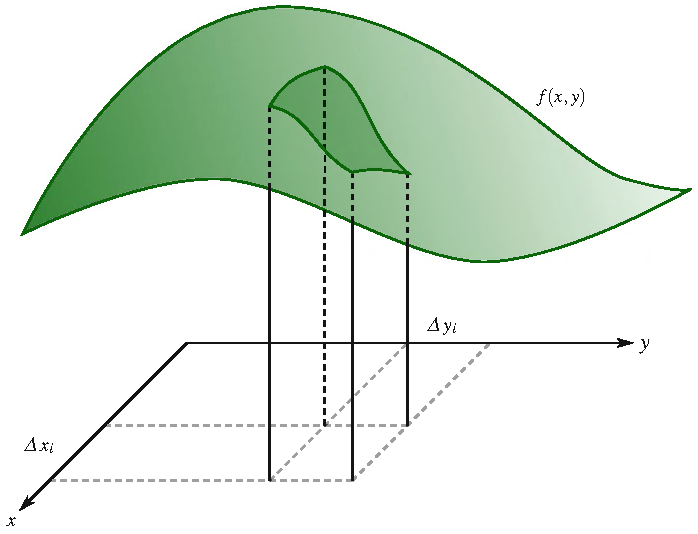
\includegraphics[width=0.827\linewidth]{images/vector/fig-7-1.pdf}
  \caption{$f(x,y)$ 图像下方、矩形 $\Delta x_i\Delta y_j$ 上方的体积}
  \label{fig:7-1}
\end{figure}

\begin{figure}[htbp]
  \centering
  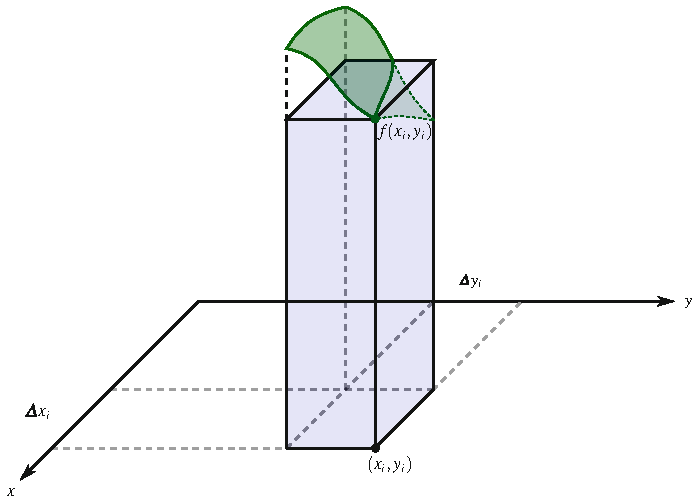
\includegraphics[width=0.827\linewidth]{images/vector/fig-7-2.pdf}
  \caption{$f(x,y)$ 图像下方、矩形 $\Delta x_i\Delta y_j$ 上方的近似体积，由乘积 $f(x_i,y_j)\Delta x_i\Delta y_j$ 给出，以蓝色显示}
  \label{fig:7-2}
\end{figure}

现在，我们基本上将以一种更适合微分形式情形的方式，同时复制上面的思想与过程，从而给出微分形式 $\alpha=f(x,y)\,dx\wedge dy$ 在区域 $R\subset\mathbb{R}^2$ 上积分的理论定义. 不过我们要提醒，这里给出的确切过程隐含地依赖于我们仍然处于欧几里得流形 $\mathbb{R}^2$ 这一事实. 对 $\mathbb{R}^n$ 的更一般定义当然是可能的，但它要求更加注意记号，而那会掩盖基本思想.

\begin{enumerate}
  \item 选择一组覆盖区域 $R$ 的等间距格点 $\{x_i\}_{i=1}^{n}$ 和 $\{y_j\}_{j=1}^{m}$. 这组格点给出点 $(x_i,y_j)\in\mathbb{R}^2_{xy}$.
  \item 对每个 $i,j$ 定义向量
  \[
  V^1_{i,j}=\binom{x_{i+1}-x_i}{0}_{(x_i,y_j)},\qquad
  V^2_{i,j}=\binom{0}{y_{j+1}-y_j}_{(x_i,y_j)}.
  \]
  注意，我们可以把向量 $V^1_{i,j}$ 和 $V^2_{i,j}$ 看作切空间 $T_{(x_i,y_j)}\mathbb{R}^2$ 的元素. 见图~\ref{fig:7-3}. 这里我们隐式地假定我们处于欧几里得情形，可以作出这一等同. 于是我们得到类似图~\ref{fig:7-4} 的情形.
  \item 对每个 $i,j$，计算 $f(x_i,y_j)\,dx\wedge dy\bigl(V^1_{i,j},V^2_{i,j}\bigr)$.
  \item 对 $i$ 和 $j$ 求和：$\sum_i\sum_j f(x_i,y_j)\,dx\wedge dy\bigl(V^1_{i,j},V^2_{i,j}\bigr)$.
  \item 取这个二重和当 $m,n\to\infty$ 时的极限，即当 $|x_{i+1}-x_i|,|y_{j+1}-y_j|\to 0$ 时的极限，并将其定义为 $\iint_R f\,dx\wedge dy$. 也就是说，
  \[
  \iint_R f\,dx\wedge dy\equiv\lim_{m,n\to\infty}\sum_{i=1}^{n}\sum_{j=1}^{m}f(x_i,y_j)\,dx\wedge dy\bigl(V^1_{i,j},V^2_{i,j}\bigr).
  \]
\end{enumerate}

\begin{figure}[htbp]
  \centering
  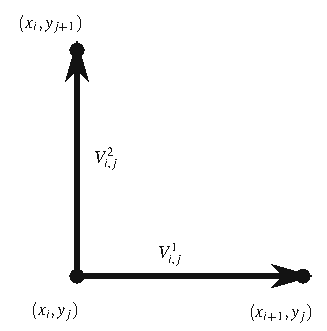
\includegraphics[width=0.481\linewidth]{images/vector/fig-7-3.pdf}
  \caption{向量 $V^1_{i,j}$ 与 $V^2_{i,j}$. 尽管它们的定义方式如此，我们还是可以把 $V^1_{i,j},V^2_{i,j}$ 视为 $T_{(x_i,y_j)}\mathbb{R}^2$ 的元素}
  \label{fig:7-3}
\end{figure}

\begin{figure}[htbp]
  \centering
  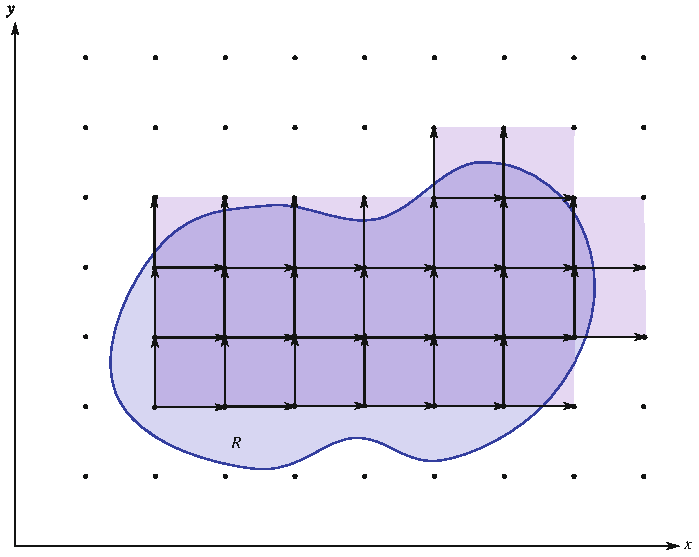
\includegraphics[width=0.829\linewidth]{images/vector/fig-7-4.pdf}
  \caption{区域 $R\subset\mathbb{R}^2$，连同覆盖它的等间距格点 $\{x_i\}_{i=1}^{n}$、$\{y_j\}_{j=1}^{m}$，以及区域 $R$ 中每个点的向量 $V^1_{i,j}$ 与 $V^2_{i,j}$. 当格点靠得越来越近，即当 $|x_{i+1}-x_i|,|y_{j+1}-y_j|\to 0$ 时，区域 $R$ 被越来越精确地近似}
  \label{fig:7-4}
\end{figure}

请比较并对照这两个过程. 它们本质上是一样的，除了求面积的方式. 在第一个过程的第 2 步中，我们只是求出数 $\Delta x_i$ 和 $\Delta y_j$，而在第二个过程中我们求出向量 $V^1_{i,j}$ 和 $V^2_{i,j}$. 然后，在第一个过程的第 3 步中，我们只是通过求乘积 $\Delta x_i\Delta y_j$ 来求流形中矩形的面积，而在第二个过程中我们用面积形式 $dx\wedge dy$ 和向量 $V^1_{i,j},V^2_{i,j}$ 来求面积，即我们求出 $dx\wedge dy\bigl(V^1_{i,j},V^2_{i,j}\bigr)$. 本质上，这就是两个过程之间仅有的差别. 但请注意，在第一个过程中我们定义的积分是 $\iint_R f(x,y)\,dx\,dy$，而在第二个过程中我们定义的积分是 $\iint_R f(x,y)\,dx\wedge dy$. 正因为如此，人们有时会把微分形式 $f(x,y)\,dx\wedge dy$ 的积分直接定义为
\[
\iint_R f(x,y)\,dx\wedge dy\equiv\iint_R f(x,y)\,dx\,dy,
\]
而不是按第二个过程用 Riemann 和来定义. 这里唯一的问题是，第一个过程及其相关的积分 $\iint_R f(x,y)\,dx\,dy$ 不记录定向，而第二个过程及其相关的积分 $\iint_R f(x,y)\,dx\wedge dy$ 记录\newterm{orientation}{定向}{orientation}.

\begin{question}\label{q:7-1}
以上面五步为指导，用 Riemann 和定义微分形式
\[
\alpha=f(x_1,x_2,\ldots,x_n)\,dx_1\wedge dx_2\wedge\cdots\wedge dx_n
\]
在区域 $R\subset\mathbb{R}^n$ 上的积分.
\end{question}

现在，假定我们发现求积分 $\int_R f(x_1,\ldots,x_n)\,dx_1\wedge\cdots\wedge dx_n$，或者等价地求积分 $\int_R f(x_1,\ldots,x_n)\,dx_1\cdots dx_n$，是困难的，但我们注意到，通过做一次适当的变量替换它会变得容易，
\[
\mathbb{R}^n_{x_1x_2\cdots x_n}\xrightarrow{\ \varphi\ }\mathbb{R}^n_{\varphi_1\varphi_2\cdots\varphi_n},\qquad(x_1,x_2,\ldots,x_n)\longmapsto(\varphi_1,\varphi_2,\ldots,\varphi_n).
\]
我们想在微分形式的语境下，从第一原理，即从 Riemann 和的定义，推导出这个变量替换公式. 换言之，我们要证明
\[
\int_R f\,dx_1\wedge\cdots\wedge dx_n=\int_{\varphi(R)}f\circ\varphi^{-1}\,T^*\varphi^{-1}\cdot\bigl(dx_1\wedge\cdots\wedge dx_n\bigr).
\]
通过做变量替换 $\varphi$，我们把 $R\subset\mathbb{R}^n_{x_1x_2\cdots x_n}$ 映到 $\varphi(R)\subset\mathbb{R}^n_{\varphi_1\varphi_2\cdots\varphi_n}$. 我们还需要假定 $\varphi$ 有逆 $\varphi^{-1}$.

\begin{enumerate}
  \item 在 $\mathbb{R}^n_{x_1x_2\cdots x_n}$ 上选择一组格点 $\{(x_{i_1},\ldots,x_{i_n})\}$. 这又给出新坐标系 $\mathbb{R}^n_{\varphi_1\varphi_2\cdots\varphi_n}$ 中的一组格点
  \[
  \Bigl\{\bigl(\varphi_1(x_{i_1},\ldots,x_{i_n}),\ldots,\varphi_n(x_{i_1},\ldots,x_{i_n})\bigr)\Bigr\}=\{(\varphi_1,\ldots,\varphi_n)\},
  \]
  见图~\ref{fig:7-5}.

  \begin{figure}[htbp]
    \centering
    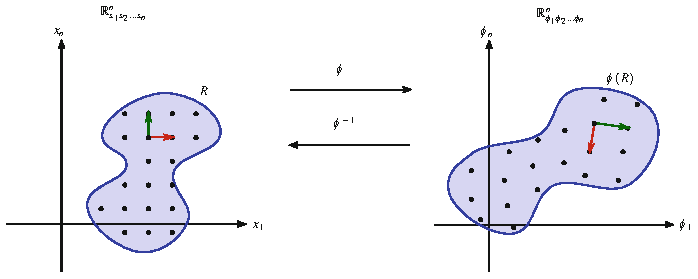
\includegraphics[width=0.960\linewidth]{images/vector/fig-7-5.pdf}
    \caption{$\mathbb{R}^n_{x_1x_2\cdots x_n}$ 中的格点 $\{(x_{i_1},\ldots,x_{i_n})\}$ 产生 $\mathbb{R}^n_{\varphi_1\varphi_2\cdots\varphi_n}$ 中的格点 $\{(\varphi_1,\ldots,\varphi_n)\}$. 图中显示了两个向量的前推}
    \label{fig:7-5}
  \end{figure}

  \item 对每个 $i_1,\ldots,i_n$ 定义向量
  \[
  V^1_{i_1\cdots i_n}=\begin{bmatrix}x_{i_1+1}-x_{i_1}\\0\\\vdots\\0\end{bmatrix}_{(x_{i_1},x_{i_2},\ldots,x_{i_n})},\quad\cdots\quad
  V^n_{i_1\cdots i_n}=\begin{bmatrix}0\\\vdots\\0\\x_{i_n+1}-x_{i_n}\end{bmatrix}_{(x_{i_1},x_{i_2},\ldots,x_{i_n})}.
  \]
  注意，由于流形是一个与切空间同构的向量空间，我们可以断言向量
\[
V^1_{i_1\cdots i_n},\ldots,V^n_{i_1\cdots i_n}\in T_{(x_{i_1},\ldots,x_{i_n})}\mathbb{R}^n_{x_1\cdots x_n}.
\]
由向量 $V^1_{i_1\cdots i_n},\ldots,V^n_{i_1\cdots i_n}$ 张成的平行六面体的体积由
  \[
  dx_1\wedge\cdots\wedge dx_n\bigl(V^1_{i_1\cdots i_n},\ldots,V^n_{i_1\cdots i_n}\bigr)
  \]
  给出.
  \item 位于 $n$ 维平行六面体上方、$f$ 图像下方的 $(n+1)$ 维体积由
  \[
  f(x_{i_1},\ldots,x_{i_n})\,dx_1\wedge\cdots\wedge dx_n\bigl(V^1_{i_1\cdots i_n},\ldots,V^n_{i_1\cdots i_n}\bigr)
  \]
  近似. 接下来，在每个格点 $p=\{(x_{i_1},\ldots,x_{i_n})\}\in\mathbb{R}^n_{x_1\cdots x_n}$ 处，该点的向量 $V^1_{i_1\cdots i_n},\ldots,V^n_{i_1\cdots i_n}$ 的前推为
  \[
  T_p\varphi\cdot V^1_{i_1\cdots i_n},\ldots,T_p\varphi\cdot V^n_{i_1\cdots i_n}\in T_{\varphi(p)}\mathbb{R}^n_{\varphi_1\varphi_2\cdots\varphi_n}.
  \]
  另外注意，对每个 $i$，有 $T\varphi^{-1}\cdot T\varphi\cdot V^i_{i_1\cdots i_n}=V^i_{i_1\cdots i_n}$，所以按定义我们有
  \begin{align*}
  &T^*\varphi^{-1}\cdot\bigl(dx_1\wedge\cdots\wedge dx_n\bigr)\\
  &\qquad\qquad\qquad\Bigl(T\varphi\cdot V^1_{i_1\cdots i_n},\ldots,T\varphi\cdot V^n_{i_1\cdots i_n}\Bigr)\\
  &=dx_1\wedge\cdots\wedge dx_n\Bigl(T\varphi^{-1}\cdot T\varphi\cdot V^1_{i_1\cdots i_n},\\
  &\qquad\qquad\qquad\qquad\ldots,T\varphi^{-1}\cdot T\varphi\cdot V^n_{i_1\cdots i_n}\Bigr)\\
  &=dx_1\wedge\cdots\wedge dx_n\Bigl(V^1_{i_1\cdots i_n},\ldots,V^n_{i_1\cdots i_n}\Bigr).
  \end{align*}
  接着，我们注意到 $f(x_{i_1},\ldots,x_{i_n})=f\circ\varphi^{-1}\circ\varphi(x_{i_1},\ldots,x_{i_n})$. 把这两者结合起来，我们有
  \begin{align*}
  &f(x_{i_1},\ldots,x_{i_n})\,dx_1\wedge\cdots\wedge dx_n\Bigl(V^1_{i_1\cdots i_n},\ldots,V^n_{i_1\cdots i_n}\Bigr)\\
  &=f\circ\varphi^{-1}\circ\varphi(x_{i_1},\ldots,x_{i_n})\,T^*\varphi^{-1}\cdot\bigl(dx_1\wedge\cdots\wedge dx_n\bigr)\Bigl(T\varphi\cdot V^1_{i_1\cdots i_n},\ldots,T\varphi\cdot V^n_{i_1\cdots i_n}\Bigr)\\
  &=f\circ\varphi^{-1}(\varphi_1,\ldots,\varphi_n)\,T^*\varphi^{-1}\cdot\bigl(dx_1\wedge\cdots\wedge dx_n\bigr)\Bigl(T\varphi\cdot V^1_{i_1\cdots i_n},\ldots,T\varphi\cdot V^n_{i_1\cdots i_n}\Bigr).
  \end{align*}
  注意，在上面最后一个等式中我们写
  \[
  \varphi(x_{i_1},\ldots,x_{i_n})=\Bigl(\varphi_1(x_{i_1},\ldots,x_{i_n}),\ldots,\varphi_n(x_{i_1},\ldots,x_{i_n})\Bigr)=(\varphi_1,\ldots,\varphi_n).
  \]
  \item 现在我们对所有 $i_1,\ldots,i_n$ 求和，得到
  \begin{align*}
  &\sum_{i_1,\ldots,i_n}f(x_{i_1},\ldots,x_{i_n})\,dx_1\wedge\cdots\wedge dx_n\Bigl(V^1_{i_1\cdots i_n},\ldots,V^n_{i_1\cdots i_n}\Bigr)\\
  &=\sum_{i_1,\ldots,i_n}f\circ\varphi^{-1}(\varphi_1,\ldots,\varphi_n)\,T^*\varphi^{-1}\bigl(dx_1\wedge\cdots\wedge dx_n\bigr)\Bigl(T\varphi\cdot V^1_{i_1\cdots i_n},\ldots,T\varphi\cdot V^n_{i_1\cdots i_n}\Bigr).
  \end{align*}
  \item 取当 $|x_{i_j+1}-x_{i_j}|\to 0$（$j=1,\ldots,n$）时的极限，我们定义
  \[
  \begin{aligned}
  \int_R f(x_1,\ldots,x_n)\,dx_1\wedge\cdots\wedge dx_n
  &=\lim_{|x_{i_j+1}-x_{i_j}|\to 0}\sum_{i_1,\ldots,i_n}f(x_{i_1},\ldots,x_{i_n})\,dx_1\wedge\cdots\wedge dx_n\\
  &\qquad\qquad\qquad\qquad\qquad\Bigl(V^1_{i_1\cdots i_n},\ldots,V^n_{i_1\cdots i_n}\Bigr)
  \end{aligned}
  \]
  以及
  \[
  \begin{aligned}
  \int_{\varphi(R)}f\circ\varphi^{-1}(\varphi_1,\ldots,\varphi_n)\,T^*\varphi^{-1}
  &=\lim_{|x_{i_j+1}-x_{i_j}|\to 0}\sum_{i_1,\ldots,i_n}f\circ\varphi^{-1}(\varphi_1,\ldots,\varphi_n)\\
  &\qquad\qquad T^*\varphi^{-1}\cdot\bigl(dx_1\wedge\cdots\wedge dx_n\bigr)\Bigl(T\varphi\cdot V^1_{i_1\cdots i_n},\\
  &\qquad\qquad\qquad\qquad\ldots,T\varphi\cdot V^n_{i_1\cdots i_n}\Bigr).
  \end{aligned}
  \]
  把第 (4) 步与这些定义结合起来，就给出下面的等式：
  \[
  \begin{aligned}
  \text{变量替换公式}\\
  &\int_R f(x_1,\ldots,x_n)\,dx_1\wedge\cdots\wedge dx_n\\
  &=\int_{\varphi(R)}f\circ\varphi^{-1}(\varphi_1,\ldots,\varphi_n)\\
  &\qquad\qquad\qquad\qquad\cdot T^*\varphi^{-1}\bigl(dx_1\wedge\cdots\wedge dx_n\bigr).
  \end{aligned}
  \]
\end{enumerate}

让我们更仔细地考察这个等式. 左边相当直接：积分在 $x_1\cdots x_n$-坐标中进行，我们在区域 $R$ 上用与 $x_1\cdots x_n$-坐标相联系的体积形式 $dx_1\wedge\cdots\wedge dx_n$ 积分函数 $f(x_1,\ldots,x_n)$. 现在，让我们拆开这个等式的右边. 首先，我们有坐标变换 $\varphi:\mathbb{R}^n\to\mathbb{R}^n$，
\begin{align*}
\mathbb{R}^n_{x_1x_2\cdots x_n}\xrightarrow{\ \varphi\ }\mathbb{R}^n_{\varphi_1\varphi_2\cdots\varphi_n}, \\
(x_1,x_2,\ldots,x_n)\longmapsto(\varphi_1,\varphi_2,\ldots,\varphi_n),
\end{align*}
它给出图~\ref{fig:7-6} 中的图像. 我们在 $\mathbb{R}^n_{x_1x_2\cdots x_n}$ 中积分的区域是 $R$，我们在 $\mathbb{R}^n_{\varphi_1\varphi_2\cdots\varphi_n}$ 中积分的区域是它的像 $\varphi(R)$. 函数 $f:\mathbb{R}^n\to\mathbb{R}$ 是变量 $x_1,x_2,\ldots,x_n$ 的函数，而函数 $f\circ\varphi^{-1}:\mathbb{R}^n\to\mathbb{R}$ 是变量 $\varphi_1,\varphi_2,\ldots,\varphi_n$ 的函数. 最后，$dx_1\wedge\cdots\wedge dx_n$ 是 $\mathbb{R}^n_{x_1x_2\cdots x_n}$ 上的面积形式. 但请注意，右边的形式是 $T^*\varphi^{-1}\cdot\bigl(dx_1\wedge\cdots\wedge dx_n\bigr)$，即面积形式 $dx_1\wedge\cdots\wedge dx_n$ 由 $\varphi^{-1}$ 的\newterm{pull-back}{拉回}{pull-back}，而不是面积形式 $d\varphi_1\wedge\cdots\wedge d\varphi_n$. 在做变量替换时，这是本质的一点.

\begin{figure}[htbp]
  \centering
  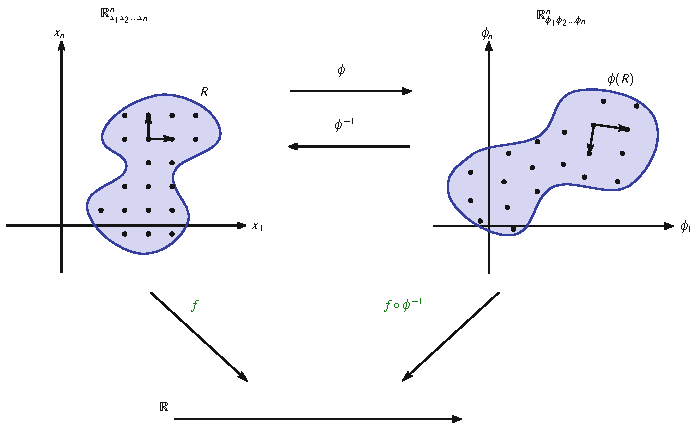
\includegraphics[width=0.960\linewidth]{images/vector/fig-7-6.pdf}
  \caption{当我们做变量替换时，必须改变积分中的三样东西：区域（蓝色）、函数（绿色）和体积形式（红色）. 左边的向量被 $T\varphi$ 前推到右边的向量}
  \label{fig:7-6}
\end{figure}

现在还有最后一个问题需要我们简要提及. 无论你是否上过入门分析课程、是否见过 Fubini 定理的证明，或者之前是否听说过 Fubini 定理，你无疑都知道它的结论. 假定我们有一个矩形区域 $R=\{a\leq x\leq b,\ c\leq y\leq d\}$ 和一个连续函数 $f:R\to\mathbb{R}$，那么 Fubini 定理断言
\[
\int_a^b\int_c^d f(x,y)\,dy\,dx=\int_c^d\int_a^b f(x,y)\,dx\,dy.
\]
它基本上是说我们可以交换积分顺序. 这实际上要求我们的函数 $f$ 在某种意义上是``好的''. 我们不想在这里深入技术细节（把它留给你分析课程），只需说你要处理的大部分函数事实上都是``好的''. 然而，在微分形式的语境下，我们当然有 $dx\wedge dy=-dy\wedge dx$，所以我们会有
\[
\int_a^b\int_c^d f(x,y)\,dy\wedge dx=-\int_c^d\int_a^b f(x,y)\,dx\wedge dy,
\]
除非你也同时改变矩形 $R$ 的定向. 这个问题以后还会再次出现，但我们不会在上面花太多时间. 一般而言，用微分形式积分会考虑定向，而微积分中是不考虑的. 因此，你的答案可能会相差一个符号.

\section{一个简单的例子}

现在，我们通过考察一个使用与第 6.1 节中相同的坐标变换的简单例子，来应用我们刚刚所做的，看看体积形式在变量替换的积分中所扮演的角色. 我们首先在 $\mathbb{R}^2_{xy}$ 的一个给定区域上积分一个函数. 然后我们应用变量替换公式，在 $\mathbb{R}^2_{uv}$ 上完成积分. 我们还将隐式地使用下面的等同：
\[
\iint_R f(x,y)\,dx\,dy\equiv\iint_R f(x,y)\,dx\wedge dy.
\]
假定我们想在由直线 $x=0$、$y=0$ 和 $y=x-2$ 围成的 $\mathbb{R}^2$ 中的区域上积分函数 $f(x,y)=x$，如图~\ref{fig:7-7} 所示. 我们首先关于 $x$ 积分，然后关于 $y$ 积分，
\begin{align*}
\int_{-2}^{0}\int_{y+2}^{0}x\,dx\,dy
&=\int_{-2}^{0}\left.\frac{x^2}{2}\right|_{y+2}^{0}dy\\
&=\int_{-2}^{0}\frac{-(y+2)^2}{2}\,dy\\
&=\int_{-2}^{0}-\frac{y^2+4y+4}{2}\,dy\\
&=-\left.\left(\frac{y^3}{6}+y^2+2y\right)\right|_{-2}^{0}\\
&=-\frac{4}{3}.
\end{align*}

\begin{figure}[htbp]
  \centering
  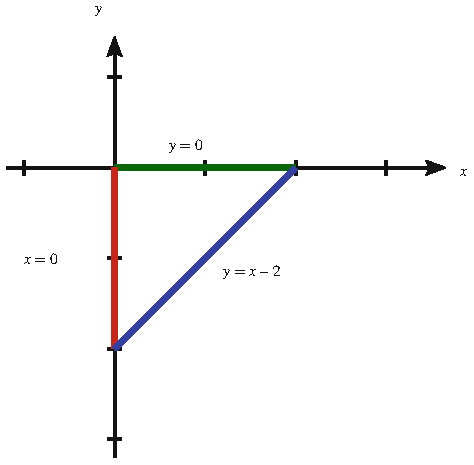
\includegraphics[width=0.568\linewidth]{images/vector/fig-7-7.pdf}
  \caption{由直线 $x=0$、$y=0$ 和 $y=x-2$ 围成的 $\mathbb{R}^2$ 中的区域.}
  \label{fig:7-7}
\end{figure}

现在我们要做同一个积分，只不过在不同坐标中. 为此我们必须利用我们在第 7.1 节中推导出的变量替换公式，
\[
\int_R f(x_1,\ldots,x_n)\,dx_1\wedge\cdots\wedge dx_n=\int_{\varphi(R)}f\circ\varphi^{-1}(\varphi_1,\ldots,\varphi_n)\,T^*\varphi^{-1}\cdot\bigl(dx_1\wedge\cdots\wedge dx_n\bigr).
\]
对我们的具体例子而言，一般的变量替换公式简化为
\[
\iint_R f(x,y)\,dx\wedge dy=\iint_{\varphi(R)}f\circ\varphi^{-1}(u,v)\,T^*\varphi^{-1}\cdot(dx\wedge dy).
\]
所有这一切归结为：当我们做变量替换时，必须改变积分中的三样东西——区域（蓝色）、函数（绿色）和体积形式（红色）. 见图~\ref{fig:7-8}.

\begin{figure}[htbp]
  \centering
  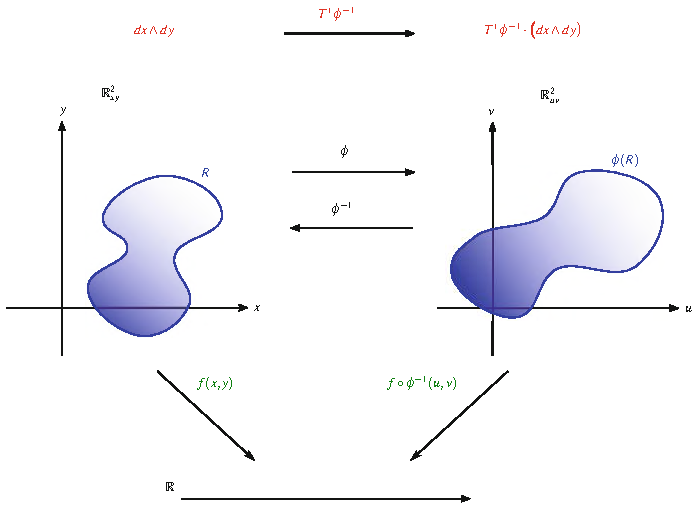
\includegraphics[width=0.948\linewidth]{images/vector/fig-7-8.pdf}
  \caption{当我们做变量替换时，必须改变积分中的三样东西：区域（蓝色）、函数（绿色）和体积形式（红色）}
  \label{fig:7-8}
\end{figure}

回到我们的例子，我们将变量替换为由 $u=x+y$ 和 $v=x-y$ 定义的 $uv$-坐标系. 换言之，我们将使用坐标变换 $\varphi:\mathbb{R}^2_{xy}\to\mathbb{R}^2_{uv}$，它由 $\varphi(x,y)=\bigl(u(x,y),v(x,y)\bigr)=(x+y,x-y)$ 给出. 我们逐一考虑需要改变的三样东西. 首先考虑我们在 $\mathbb{R}^2_{uv}$ 中积分的区域. 坐标变换 $u=x+y$ 和 $v=x-y$ 可以改写为 $x=\frac{u+v}{2}$，$y=\frac{u-v}{2}$，这意味着在变换下，定义边界的方程变为
\begin{align*}
x=0&\Rightarrow u=-v,\\
y=0&\Rightarrow u=v,\\
y=x-2&\Rightarrow v=2.
\end{align*}
于是我们的区域在 $\mathbb{R}^2_{uv}$ 中的像如图~\ref{fig:7-9} 所示.

\begin{figure}[htbp]
  \centering
  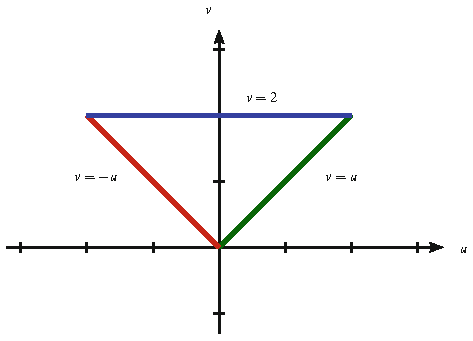
\includegraphics[width=0.599\linewidth]{images/vector/fig-7-9.pdf}
  \caption{图~\ref{fig:7-7} 中的区域在变换 $\varphi(x,y)=\bigl(u(x,y),v(x,y)\bigr)=(x+y,x-y)$ 下于 $\mathbb{R}^2_{uv}$ 中的像}
  \label{fig:7-9}
\end{figure}

其次，我们考虑函数. 我们要积分的函数 $f(x,y)=x$ 变换为 $f\circ\varphi^{-1}(u,v)=\frac{u+v}{2}$. 第三，我们需要考虑体积形式如何变化. 回想映射 $\varphi^{-1}$ 诱导拉回映射 $T^*\varphi^{-1}$，
\begin{align*}
\mathbb{R}^2_{uv}\xrightarrow{\ \varphi^{-1}\ }\mathbb{R}^2_{xy},\qquad(u,v)\longmapsto(x,y),\qquad
T^*\varphi^{-1}:\Lambda^2\bigl(\mathbb{R}^2_{xy}\bigr)\xleftarrow{\ }\Lambda^2\bigl(\mathbb{R}^2_{uv}\bigr), \\
T^*\varphi^{-1}\cdot dx\wedge dy\longmapsto dx\wedge dy.
\end{align*}
在第 6 章中我们已经求得
\[
T^*\varphi^{-1}\cdot\bigl(dx\wedge dy\bigr)=-\frac{1}{2}\,du\wedge dv.
\]

\begin{figure}[htbp]
  \centering
  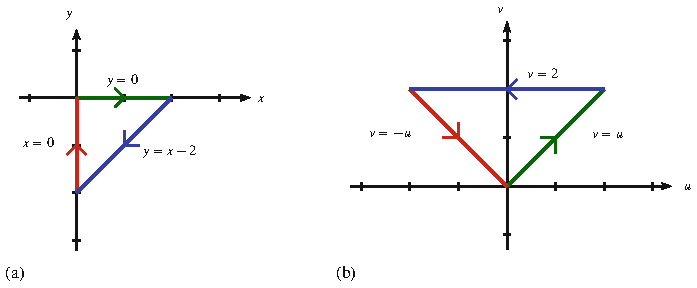
\includegraphics[width=0.909\linewidth]{images/vector/fig-7-10.pdf}
  \caption{映射 $\varphi:\mathbb{R}^2_{xy}\to\mathbb{R}^2_{uv}$（$\varphi(x,y)=\bigl(u(x,y),v(x,y)\bigr)=(x+y,x-y)$）对我们要积分的区域的影响. (a) $\mathbb{R}^2_{xy}$ 中包围的面积为 $2$，定向为顺时针. (b) $\mathbb{R}^2_{uv}$ 中包围的面积为 $4$，定向为逆时针}
  \label{fig:7-10}
\end{figure}

在变换 $\varphi$ 下，区域的各个角按如下方式映射：
\[
\begin{array}{c}
\mathbb{R}^2_{xy}\xrightarrow{\ \varphi\ }\mathbb{R}^2_{uv}\\
(x,y)\longmapsto(x+y,x-y)\equiv(u,v)\\
(0,0)\longmapsto(0,0)\\
(2,0)\longmapsto(2,2)\\
(0,-2)\longmapsto(-2,2).
\end{array}
\]
于是我们可以看出，当我们沿区域绕行时，$\mathbb{R}^2_{uv}$ 中的定向与 $\mathbb{R}^2_{xy}$ 中的定向是不同的. 另外，请比较图~\ref{fig:7-10} 中两个区域的面积. 这张图清楚地说明了为什么我们需要使用面积形式的拉回. 在变量替换下，我们要积分的区域的面积和定向都会改变. 通过使用面积形式的拉回，我们补偿了这些变化. 微分形式，特别是体积形式，随身携带着我们做积分问题的变量替换所需的信息.

总之，$\iint_R x\,dx\,dy$ 确实应该被想成 $\iint_R x\,dx\wedge dy$. 当我们改变坐标时，区域 $R=\{(x,y)\,|\,0\leq x\leq 2,\ x-2\leq y\leq 0\}$ 变成 $\widetilde{R}=\{(u,v)\,|\,0\leq v\leq 2,\ -v\leq u\leq v\}$，$f(x,y)=x$ 变成 $\widetilde{f}(u,v)=\frac{u+v}{2}$，而 $dx\,dy$——它实际上是 $dx\wedge dy$——变成 $-\frac{1}{2}\,du\wedge dv$，或者 $-\frac{1}{2}\,du\,dv$. 换言之，我们有
\[
\iint_R f(x,y)\,dx\,dy=\iint_{\widetilde{R}}\widetilde{f}(u,v)\left(-\frac{1}{2}\right)du\,dv,
\]
这实际上是
\[
\iint_R f(x,y)\,dx\wedge dy=\iint_{\widetilde{R}}\widetilde{f}(u,v)\left(-\frac{1}{2}\right)du\wedge dv.
\]
现在让我们在变换后的区域上积分变换后的函数，
\begin{align*}
\int_0^2\int_{-v}^{v}\frac{u+v}{2}\left(-\frac{1}{2}\right)du\,dv
&=\int_0^2\left.\left(-\frac{1}{2}\right)\left(\frac{u^2}{4}+\frac{uv}{2}\right)\right|_{-v}^{v}dv\\
&=\left(-\frac{1}{2}\right)\int_0^2 v^2\,dv\\
&=\left(-\frac{1}{2}\right)\left.\frac{v^3}{3}\right|_0^2\\
&=\left(-\frac{1}{2}\right)\frac{8}{3}\\
&=-\frac{4}{3}.
\end{align*}
通常，变量替换（也称为换基）会使我们要积分的函数简单得多，从而使积分更容易. 为了看一个例子，假定我们想在和之前相同的区域 $R=\{(x,y)\,|\,0\leq x\leq 2,\ x-2\leq y\leq 0\}$ 上积分 $f(x,y)=e^{\frac{x+y}{x-y}}$. 希望简化这个函数、从而简化积分的愿望，正是选择新坐标 $u=x+y$ 和 $v=x-y$ 的动机，
\begin{align*}
\int_{-2}^{0}\int_{y+2}^{0}e^{\frac{x+y}{x-y}}dx\,dy
&=\int_{-2}^{0}\int_{y+2}^{0}e^{\frac{x+y}{x-y}}dx\wedge dy\\
&=\int_0^2\int_{-v}^{v}e^{\frac{u}{v}}\left(-\frac{1}{2}\right)du\wedge dv\\
&=\int_0^2\int_{-v}^{v}e^{\frac{u}{v}}\left(-\frac{1}{2}\right)du\,dv\\
&=\left(-\frac{1}{2}\right)\int_0^2\left.\left[ve^{\frac{u}{v}}\right]\right|_{-v}^{v}dv\\
&=\left(-\frac{1}{2}\right)\int_0^2 v\left(e^{\frac{v}{v}}-e^{-\frac{v}{v}}\right)dv\\
&=\left(-\frac{1}{2}\right)\left(e^1-e^{-1}\right)\int_0^2 v\,dv\\
&=\left(-\frac{1}{2}\right)\left(e^1-e^{-1}\right)\left.\frac{v^2}{2}\right|_0^2\\
&=-\left(e^1-e^{-1}\right)\\
&\approx-2.35.
\end{align*}
显然，对所有 $x$ 和 $y$ 都有 $e^{\frac{x+y}{x-y}}>0$，所以你是在一个你通常认为是正的区域上积分一个正的函数，因此你很自然地期望得到一个正的体积，而不是负的. 当然，以这种方式思考时，我们没有考虑空间的``定向''. 但人们自然期望体积为正这一事实，正是经典微积分课程中对多余的那一项——Jacobian，在这里是 $-\frac{1}{2}$——取绝对值的原因. 本质上这相当于约定：无论坐标变换过程中发生了什么，我们总是假定我们的坐标轴遵循``右手法则''.

然而，当我们开始处理更高级、更抽象的数学时，我们希望能够记录流形的定向，而这正是微分形式所做的. 回想一下，微分形式记录定向这一事实全部源于我们的楔积是用行列式定义的，而行列式本身——按照我们展开它的方式——记录定向. 在我们的例子中出现负号，是因为当我们用变换把两个向量从 $xy$ 平面前推到 $uv$ 平面时，像向量改变了``手性''，因此正定向的区域变成负定向的区域，反之亦然.

\section{极坐标、柱坐标与球坐标}

现在我们将考察一系列涉及极坐标、柱坐标和球坐标的例子. 尽管你在微积分中见过这些坐标系，这里的讲述将把你已经知道的东西与微分形式的视角联系起来.

\subsection{极坐标例子}

现在，让我们动手处理一个涉及极坐标的实际例子. 假定我们想求由 $z=0$ 平面和抛物面 $z=3-x^2-y^2$ 围成的三维立体的体积，见图~\ref{fig:7-11}. 首先我们求抛物面与 $z=0$ 平面的交线，
\[
z=0\Rightarrow 0=3-x^2-y^2\Rightarrow x^2+y^2=3,
\]
它给出 $xy$ 平面中的区域 $R=\{x^2+y^2\leq 3\}$. 于是我们要计算的积分是
\[
\int_R 3-x^2-y^2\,dx\wedge dy,
\]
或者用更传统的微积分记号，
\[
\int_{-\sqrt{3}}^{\sqrt{3}}\int_{-\sqrt{3-y^2}}^{\sqrt{3-y^2}}\bigl(3-x^2-y^2\bigr)dx\,dy.
\]
毫无疑问，这个计算会是很麻烦的.

\begin{figure}[htbp]
  \centering
  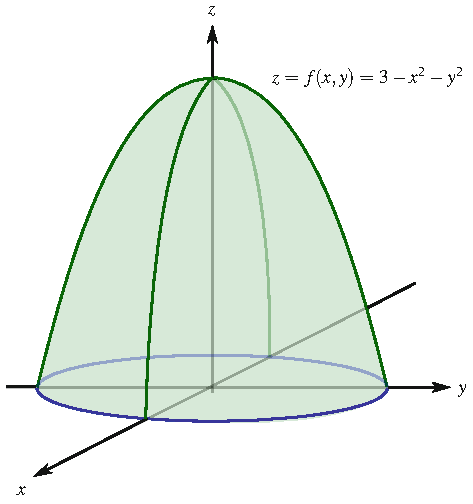
\includegraphics[width=0.561\linewidth]{images/vector/fig-7-11.pdf}
  \caption{由 $z=0$ 平面和抛物面 $z=3-x^2-y^2$ 围成的三维立体}
  \label{fig:7-11}
\end{figure}

\begin{question}\label{q:7-2}
尝试用你在微积分课上记得的技术完成这个积分，不做变量替换，看看你能进行到哪一步.
\end{question}

当我们实际计算积分时，在矩形区域上积分显然比其他形状的区域上积分简单得多. 由于这个区域是 $xy$ 平面中的一个圆盘，使用极坐标变换会在 $r\theta$-平面中产生一个矩形区域. 也就是说，给定极坐标变换
\[
x=r\cos\theta,\qquad y=r\sin\theta,
\]
这个区域在极坐标变换下的像是
\[
\varphi(R)=\{0\leq r\leq\sqrt{3},\ 0\leq\theta\leq 2\pi\},
\]
如图~\ref{fig:7-12} 所示.

\begin{figure}[htbp]
  \centering
  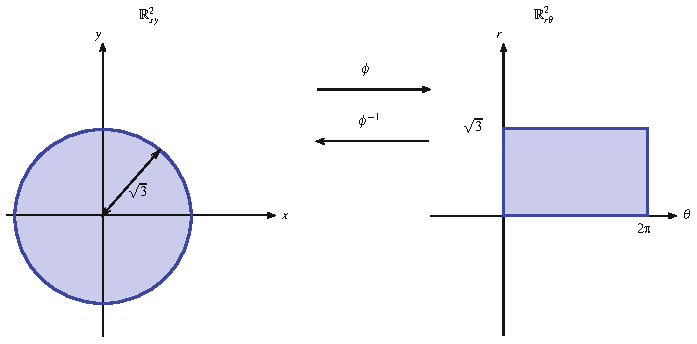
\includegraphics[width=0.907\linewidth]{images/vector/fig-7-12.pdf}
  \caption{圆形区域 $\{x^2+y^2\leq 3\}$ 在极坐标变换下的像是矩形区域 $\{0\leq r\leq\sqrt{3},\ 0\leq\theta\leq 2\pi\}$}
  \label{fig:7-12}
\end{figure}

\begin{question}\label{q:7-3}
证明区域 $\varphi(R)$ 确实是 $\{0\leq r\leq\sqrt{3},\ 0\leq\theta\leq 2\pi\}$.
\end{question}

于是我们要利用上一节从第一原理推导出的等式，用坐标变换来简化我们的积分，
\[
\int_R f\,dx_1\wedge\cdots\wedge dx_n=\int_{\varphi(R)}f\circ\varphi^{-1}\,T^*\varphi^{-1}\cdot\bigl(dx_1\wedge\cdots\wedge dx_n\bigr).
\]
在这里我们花一点时间，就我们使用的记号以及 $xy$-平面与 $r\theta$-平面的比较谈几点. 第一，微积分教材中通常给出的极坐标变换 $x=r\cos\theta$、$y=r\sin\theta$，是从 $r\theta$-平面到 $xy$-平面的变换，而不是反过来. 从 $xy$-平面到 $r\theta$-平面的变换由相当复杂的
\[
r=\sqrt{x^2+y^2},\qquad\theta=\arctan\frac{y}{x}
\]
给出. 我们还需要把 $r\theta$-平面限制在 $0<\theta<2\pi$，以便 $\arctan$ 有定义. 我们将对此稍稍放宽要求，但对我们的积分问题来说这样做不会带来麻烦. 另外，我们把哪个方向标记为 $\varphi$、哪个标记为 $\varphi^{-1}$ 当然完全是任意的，但为了与上一节的记号保持一致，我们把从 $xy$-平面到 $r\theta$-平面的变换标记为 $\varphi$，把逆变换标记为 $\varphi^{-1}$. 想一想这有点令人惊讶，但事实上拥有 $\varphi^{-1}$，即用 $r$ 和 $\theta$ 表示的 $x$ 和 $y$，使我们能轻易地求出 $\varphi(R)$ 和 $f\circ\varphi^{-1}$，
\begin{align*}
f\circ\varphi^{-1}&=3-(r\cos\theta)^2-(r\sin\theta)^2\\
&=3-r^2(\sin^2\theta+\cos^2\theta)\\
&=3-r^2.
\end{align*}
最后，我们求 $T^*\varphi^{-1}\cdot\bigl(dx\wedge dy\bigr)$. 为此我们首先注意到 $T^*\varphi^{-1}\cdot\bigl(dx\wedge dy\bigr)$ 具有某个函数 $g$ 决定的 $g(r,\theta)\,d\theta\wedge dr$ 的形式. 接着我们注意到
\begin{align*}
g(r,\theta)&=g(r,\theta)\,d\theta\wedge dr\left(\binom{1}{0},\binom{0}{1}\right)\\
&=T^*\varphi^{-1}\cdot\bigl(dx\wedge dy\bigr)\left(\binom{1}{0},\binom{0}{1}\right)\\
&=dx\wedge dy\left(T\varphi^{-1}\cdot\binom{1}{0},T\varphi^{-1}\cdot\binom{0}{1}\right).
\end{align*}
为了继续下去，我们现在需要求 $T\varphi^{-1}$，
\[
T\varphi^{-1}=\begin{bmatrix}\frac{\partial x}{\partial\theta}&\frac{\partial x}{\partial r}\\\frac{\partial y}{\partial\theta}&\frac{\partial y}{\partial r}\end{bmatrix}=\begin{bmatrix}-r\sin\theta&\cos\theta\\r\cos\theta&\sin\theta\end{bmatrix},
\]
于是我们可以计算
\begin{align*}
T\varphi^{-1}\cdot\binom{1}{0}=\begin{bmatrix}-r\sin\theta&\cos\theta\\r\cos\theta&\sin\theta\end{bmatrix}\binom{1}{0}=\binom{-r\sin\theta}{r\cos\theta}, \\
T\varphi^{-1}\cdot\binom{0}{1}=\begin{bmatrix}-r\sin\theta&\cos\theta\\r\cos\theta&\sin\theta\end{bmatrix}\binom{0}{1}=\binom{\cos\theta}{\sin\theta},
\end{align*}
这反过来给出
\begin{align*}
dx\wedge dy\left(T\varphi^{-1}\cdot\binom{1}{0},T\varphi^{-1}\cdot\binom{0}{1}\right)
&=dx\wedge dy\left(\binom{-r\sin\theta}{r\cos\theta},\binom{\cos\theta}{\sin\theta}\right)\\
&=\begin{vmatrix}-r\sin\theta&\cos\theta\\r\cos\theta&\sin\theta\end{vmatrix}\\
&=-r\sin^2\theta-r\cos^2\theta\\
&=-r,
\end{align*}
这意味着 $g(r,\theta)=-r$. 因此
\[
T^*\varphi^{-1}\cdot\bigl(dx\wedge dy\bigr)=-r\,d\theta\wedge dr.
\]
我们当然已经在上一章中求得了这一结果.

现在我们有了把积分改写为极坐标所需的全部要素. 当然，我们费了很大的劲，把每一步都事无巨细地展示出来. 一旦你这样做了几次，最终结果就现成可用，你可以直接把积分写成极坐标形式，
\begin{align*}
\int_{-\sqrt{3}}^{\sqrt{3}}\int_{-\sqrt{3-y^2}}^{\sqrt{3-y^2}}\bigl(3-x^2-y^2\bigr)dx\,dy
&=\int_R f\,dx\wedge dy\\
&=\int_{\varphi(R)}f\circ\varphi^{-1}\,T^*\varphi^{-1}\cdot(dx\wedge dy)\\
&=\int_0^{\sqrt{3}}\int_0^{2\pi}(3-r^2)(-r)\,d\theta\wedge dr\\
&=\int_0^{\sqrt{3}}\int_0^{2\pi}-3r+r^3\,d\theta\,dr.
\end{align*}
这是一个比我们一开始的那个容易得多的积分. 唯一需要注意的是面积形式 $dx\wedge dy$ 的拉回中 $r$ 前面的负号，它反映了定向的改变.

\begin{question}\label{q:7-4}
完成这个积分. 如果你设法完成了问题~\ref{q:7-2} 中的积分，答案是否相同？
\end{question}

\subsection{柱坐标例子}

现在我们将做一个积分问题，其中变量替换为柱坐标会使积分更容易. 假定我们想在由圆锥面 $z=\sqrt{x^2+y^2}$ 和平面 $z=2$ 围成的区域上积分函数 $f(x,y)=x^2+y^2$. 换言之，我们想求积分
\[
\int_R (x^2+y^2)\,dx\,dy\,dz.
\]
为了精确地画出表示这个积分的图形，我们需要四个维度，所以我们不打算那样做. 只需想象一幅类似图~\ref{fig:7-1} 的漫画. 用笛卡尔坐标写出区域 $R$ 的一种方式是
\[
R=\Bigl\{(x,y,z)\,\Bigl|\,-2\leq x\leq 2,\ -\sqrt{4-x^2}\leq y\leq\sqrt{4-x^2},\ \sqrt{x^2+y^2}\leq z\leq 2\Bigr\},
\]
它给出积分
\[
\int_{-2}^{2}\int_{-\sqrt{4-x^2}}^{\sqrt{4-x^2}}\int_{\sqrt{x^2+y^2}}^{2}(x^2+y^2)\,dz\,dy\,dx.
\]
然而，和之前一样，我们可以看出做这个积分会相当复杂.

\begin{question}\label{q:7-5}
证明由圆锥面 $z=\sqrt{x^2+y^2}$ 和平面 $z=2$ 围成的区域确实可以写成
\[
\Bigl\{-2\leq x\leq 2,\ -\sqrt{4-x^2}\leq y\leq\sqrt{4-x^2},\ \sqrt{x^2+y^2}\leq z\leq 2\Bigr\}.
\]
\end{question}

\begin{question}\label{q:7-6}
尝试用你在微积分课上记得的技术完成这个计算，不做变量替换，看看你能进行到哪一步.
\end{question}

但是当我们考虑柱坐标变换
\[
\mathbb{R}^3_{r\theta z}\xrightarrow{\ \varphi^{-1}\ }\mathbb{R}^3_{xyz},\qquad(r,\theta,z)\longmapsto(r\cos\theta,r\sin\theta,z),
\]
很明显，这个区域用柱坐标描述要简单得多，
\[
\varphi(R)=\{0\leq\theta\leq 2\pi,\ 0\leq r\leq 2,\ r\leq z\leq 2\}.
\]

\begin{figure}[htbp]
  \centering
  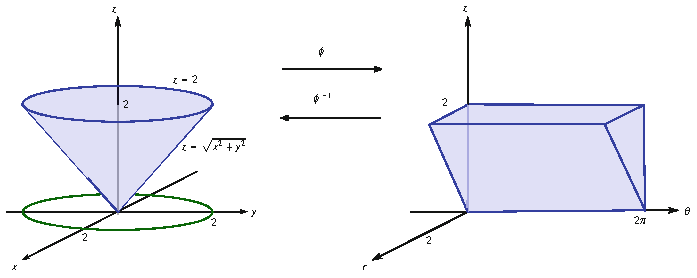
\includegraphics[width=0.960\linewidth]{images/vector/fig-7-13.pdf}
  \caption{映射 $\varphi:\mathbb{R}^3_{xyz}\to\mathbb{R}^3_{r\theta z}$ 对我们要积分的区域的影响}
  \label{fig:7-13}
\end{figure}

\begin{question}\label{q:7-7}
证明区域 $\varphi(R)$ 确实是 $\{0\leq\theta\leq 2\pi,\ 0\leq r\leq 2,\ r\leq z\leq 2\}$.
\end{question}

我们要指出，为了与上一节的记号保持一致，我们把从 $\mathbb{R}^3_{r\theta z}$ 到 $\mathbb{R}^3_{xyz}$ 的映射记为 $\varphi^{-1}$，而不是像上一章那样记为 $\varphi$. 只要我们限制映射在 $\mathbb{R}^3_{r\theta z}$ 的适当定义域上，使我们的逆有定义，那么这应该不会引起混淆. 见图~\ref{fig:7-13}. 我们还有 $f\circ\varphi^{-1}=r^2$，以及 $T^*\varphi^{-1}\cdot(dx\wedge dy\wedge dz)=-r\,d\theta\wedge dr\wedge dz$.

\begin{question}\label{q:7-8}
求出 $f\circ\varphi^{-1}$ 和 $T^*\varphi^{-1}\cdot(dx\wedge dy\wedge dz)$.
\end{question}

最后，利用上一节推导出的恒等式，我们得到
\begin{align*}
\int_R f\,dx\wedge dy\wedge dz
&=\int_{\varphi(R)}f\circ\varphi^{-1}\,T^*\varphi^{-1}\cdot\bigl(dx\wedge dy\wedge dz\bigr)\\
&=\int_{\varphi(R)}(r^2)(-r)\,d\theta\wedge dr\wedge dz\\
&=\int_{\varphi(R)}(r^2)\,r\,d\theta\wedge dz\wedge dr\\
&=\int_0^{2\pi}\int_0^2\int_r^2 r^3\,d\theta\,dz\,dr.
\end{align*}

\begin{question}\label{q:7-9}
完成这个积分.
\end{question}

\subsection{球坐标例子}

我们用一个使用球坐标的坐标变换例子来结束本节. 假定我们想在整个单位球
\[
R=\bigl\{x^2+y^2+z^2\leq 1\bigr\}
\]
上积分函数 $f(x,y,z)=e^{(x^2+y^2+z^2)^{3/2}}$. 一个能完成这件事的积分是
\[
\int_{-1}^{1}\int_{-\sqrt{1-x^2}}^{\sqrt{1-x^2}}\int_{-\sqrt{1-x^2-y^2}}^{\sqrt{1-x^2-y^2}}e^{(x^2+y^2+z^2)^{3/2}}\,dz\,dy\,dx,
\]

\begin{figure}[htbp]
  \centering
  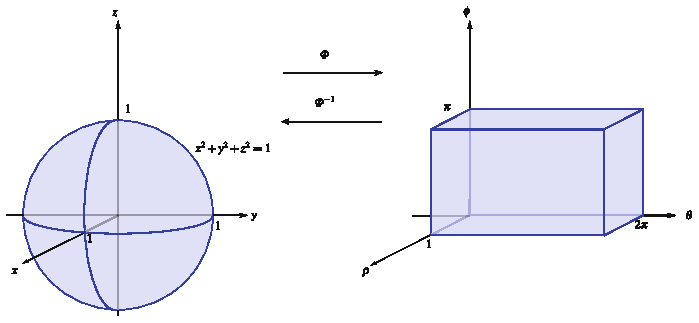
\includegraphics[width=0.960\linewidth]{images/vector/fig-7-14.pdf}
  \caption{映射 $\Phi:\mathbb{R}^3_{xyz}\to\mathbb{R}^3_{\rho\theta\varphi}$ 对我们要积分的区域的影响}
  \label{fig:7-14}
\end{figure}

它充其量显然会是很难的. 在球坐标变换
\[
\mathbb{R}^3_{\rho\theta\varphi}\xrightarrow{\ \Phi^{-1}\ }\mathbb{R}^3_{xyz},\qquad(\rho,\theta,\varphi)\longmapsto(\rho\sin\varphi\cos\theta,\rho\sin\varphi\sin\theta,\rho\cos\varphi)
\]
下，我们的区域变成
\[
\Phi(R)=\{0\leq\rho\leq 1,\ 0\leq\theta\leq 2\pi,\ 0\leq\varphi\leq\pi\}.
\]
由于 $\varphi$ 是球坐标中使用的标准变量之一，我们把映射记为大写的 $\Phi$. 见图~\ref{fig:7-14}.

\begin{question}\label{q:7-10}
证明区域 $\Phi(R)$ 确实是 $\{0\leq\rho\leq 1,\ 0\leq\theta\leq 2\pi,\ 0\leq\varphi\leq\pi\}$.
\end{question}

我们还得到 $f\circ\Phi^{-1}=e^{(\rho^2)^{3/2}}=e^{\rho^3}$，以及 $T^*\Phi^{-1}\cdot(dx\wedge dy\wedge dz)=-\rho^2\sin\varphi\,d\rho\wedge d\theta\wedge d\varphi$. 同样，利用上一节推导出的恒等式，我们有
\begin{align*}
\int_R f\,dx\wedge dy\wedge dz
&=\int_{\Phi(R)}f\circ\Phi^{-1}\,T^*\Phi^{-1}\cdot\bigl(dx\wedge dy\wedge dz\bigr)\\
&=\int_{\Phi(R)}(e^{\rho^3})(-\rho^2\sin\varphi)\,d\rho\wedge d\theta\wedge d\varphi\\
&=\int_0^{\pi}\int_0^{2\pi}\int_0^1-\rho^2e^{\rho^3}\sin\varphi\,d\rho\,d\theta\,d\varphi.
\end{align*}

\begin{question}\label{q:7-11}
完成这个积分.
\end{question}

\section{参数化曲面上微分形式的积分}

到目前为止，我们考察了一种特定类型的积分问题，即我们要积分的区域在其他某个坐标系中有更简单表示的问题. 然而，还有一些其他类型的积分问题我们可以用微分形式来做.

只要在一个 $n$ 维流形上有一个 $n$-形式，我们就可以对它积分. 例如，我们可以在曲线上积分 1-形式，在曲面上积分 2-形式，在三维空间中积分 3-形式，等等. 只要我们有流形 $\Sigma_k\subset\mathbb{R}^n$（$k<n$）的一个\newterm{parametrization}{参数化}{parametrization}，即一个可逆映射 $\varphi^{-1}:U\subset\mathbb{R}^k\to\Sigma_k\subset\mathbb{R}^n$，我们就可以用 $T^*\varphi^{-1}$ 把 $k$-形式拉回到 $U\subset\mathbb{R}^k$，并在那里积分，从而在 $\Sigma_k$ 上积分 $k$-形式. 用 $\varphi^{-1}$ 而不是 $\varphi$ 来命名参数化有点不寻常，但我们想保持与上一章一致的记号. 本节的其余部分将讨论在 $\mathbb{R}^n$ 中以参数化曲面 $\Sigma_k$ 给出的子流形上积分形式. 我们之前推导出的等式是
\[
\int_R f\,dx_1\wedge\cdots\wedge dx_n=\int_{\varphi(R)}f\circ\varphi^{-1}\,T^*\varphi^{-1}\cdot\bigl(dx_1\wedge\cdots\wedge dx_n\bigr).
\]
我们通常想使用的这个等式的形式是
\[
\text{$k$ 维参数化曲面 $\Sigma_k$ 上 $k$-形式的积分}\qquad\int_{\Sigma_k}\alpha=\int_{\varphi(\Sigma_k)}T^*\varphi^{-1}\cdot\alpha.
\]
当 $k=1$ 时，我们得到一条曲线，我们经常写 $\Sigma_1=C$.

\begin{question}\label{q:7-12}
用与第 7.1 节类似的涉及 Riemann 和的论证来定义这个公式.
\end{question}

但在那之前，我们还想重申：你可以——而且经常确实——积分各种各样不是微分形式的对象. 例如，要求 $\mathbb{R}^3$ 中二维曲面的表面积，你需要积分
\[
\sqrt{(dx\wedge dy)^2+(dy\wedge dz)^2+(dz\wedge dx)^2},
\]
这不是一个微分形式，因为它不是多重线性的，尽管它是由微分形式 $dx\wedge dy$、$dy\wedge dz$ 和 $dz\wedge dx$ 组成的. 然而，对于简单的曲面，有时这样的积分仍然可以手工完成. 否则，一般可以用数值方法求出数值答案. 形式之所以如此有用，原因之一就是广义 Stokes 定理. 不过，广义 Stokes 定理并不适用于不是形式的被积函数.

\subsection{线积分}

这里我们将考察一些涉及在一维流形上积分 1-形式的例子. 我们将利用恒等式
\[
\int_C\alpha=\int_{\varphi(C)}T^*\varphi^{-1}\cdot\alpha.
\]

\textbf{例一.} 我们从 $\mathbb{R}^2$ 中的一个例子开始. 我们将沿两条不同的曲线积分 1-形式 $y^2dx+xdy$. 第一条曲线 $C_1$ 是从 $(-5,-3)$ 到 $(0,2)$ 的线段. 第二条曲线 $C_2$ 是抛物线 $x=4-y^2$ 从 $(-5,-3)$ 到 $(0,2)$ 的弧. 我们首先计算沿 $C_1$ 的积分. 为此，我们首先要做的就是把路径 $C_1$ 参数化为 $\varphi^{-1}(t)=\bigl(x(t),y(t)\bigr)=(5t-5,5t-3)$. 令 $R=[0,1]\subset\mathbb{R}$，我们有 $\varphi^{-1}(R)=\bigl\{(x,y)\,\bigl|\,x=5t-5,\ y=5t-3,\ 0\leq t\leq 1\bigr\}=C_1$. 见图~\ref{fig:7-15}. 利用映射 $\varphi^{-1}$，我们求 $T\varphi^{-1}$，
\[
T\varphi^{-1}=\begin{bmatrix}\frac{\partial x}{\partial t}\\\frac{\partial y}{\partial t}\end{bmatrix}=\binom{5}{5},
\]
于是我们得到诱导的切映射和余切映射，
\begin{align*}
T_p(\mathbb{R})\xrightarrow{\;T\varphi^{-1}\;}T_{\varphi^{-1}(p)}\bigl(\mathbb{R}^2\bigr),\qquad[1]\in T_p(\mathbb{R})\longmapsto T\varphi^{-1}\cdot[1]=\binom{5}{5}[1]=\binom{5}{5}\in T_{\varphi^{-1}(p)}\bigl(\mathbb{R}^2\bigr), \\
T^*_p(\mathbb{R})\xleftarrow{\;T^*\varphi^{-1}\;}T^*_{\varphi^{-1}(p)}\bigl(\mathbb{R}^2\bigr),\qquad f(t)\,dt=T^*\varphi^{-1}\cdot\bigl(y^2dx+xdy\bigr)\longmapsto y^2dx+xdy,
\end{align*}
其中 $f(t)$ 是某个函数. 这个关于 $t$ 的函数正是我们想求的. 注意 $f(t)\,dt\bigl([1]\bigr)=f(t)$，所以我们有
\begin{align*}
f(t)&=f(t)\,dt\bigl([1]\bigr)\\
&=T^*\varphi^{-1}\cdot\bigl(y^2dx+xdy\bigr)\bigl([1]\bigr)\\
&=\bigl(y^2dx+xdy\bigr)\bigl(T\varphi^{-1}\cdot[1]\bigr)\\
&=\bigl(y^2dx+xdy\bigr)\binom{5}{5}\\
&=y^2dx\binom{5}{5}+xdy\binom{5}{5}\\
&=y^2(5)+x(5)\\
&=(5t-3)^2(5)+(5t-5)(5)\\
&=125t^2-125t+20,
\end{align*}
所以我们有
\[
T^*\varphi^{-1}\cdot\bigl(y^2dx+xdy\bigr)=(125t^2-125t+20)\,dt.
\]
利用下面的等式
\[
\int_C\alpha=\int_{\varphi(C)}T^*\varphi^{-1}\cdot\alpha,
\]
我们的积分变成
\begin{align*}
\int_{C_1}y^2dx+xdy
&=\int_{[0,1]}\bigl(125t^2-125t+20\bigr)dt\\
&=\int_0^1\bigl(125t^2-125t+20\bigr)dt\\
&=-\frac{5}{6}.
\end{align*}

\begin{figure}[htbp]
  \centering
  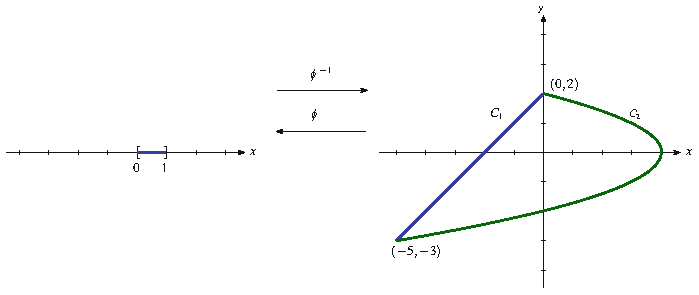
\includegraphics[width=0.960\linewidth]{images/vector/fig-7-15.pdf}
  \caption{映射 $\varphi^{-1}$ 把 $[0,1]$ 送到曲线 $C_1$}
  \label{fig:7-15}
\end{figure}

现在我们将沿第二条路径 $C_2$ 求 1-形式 $y^2dx+xdy$ 的积分. 为此，我们首先要做的就是把路径 $C_2$ 参数化为 $\varphi^{-1}(t)=\bigl(x(t),y(t)\bigr)=(4-t^2,t)$. 令 $R=[-3,2]\subset\mathbb{R}$，我们有 $\varphi^{-1}(R)=\bigl\{(x,y)\,\bigl|\,x=4-t^2,\ y=t,\ -3\leq t\leq 2\bigr\}=C_2$. 见图~\ref{fig:7-16}. 利用映射 $\varphi^{-1}$，我们求 $T\varphi^{-1}$，
\[
T_p\varphi^{-1}=\begin{bmatrix}\frac{\partial x}{\partial t}\\\frac{\partial y}{\partial t}\end{bmatrix}_p=\binom{-2t}{1}_p,
\]
这实际上是映射
\[
\begin{aligned}
&T_p(\mathbb{R})\xrightarrow{\;T\varphi^{-1}\;}T_{\varphi^{-1}(p)}\bigl(\mathbb{R}^2\bigr),\\
&\qquad[1]\in T_p(\mathbb{R})\longmapsto T_p\varphi^{-1}\cdot[1]=\binom{-2t}{1}[1]=\binom{-2t}{1}\in T_{\varphi^{-1}(p)}\bigl(\mathbb{R}^2\bigr).
\end{aligned}
\]
由此我们可以清楚地看到，映射 $T_p\varphi^{-1}$ 依赖于我们的向量所在的点. 为了使这一点更具体，我们做几个例子，说明基于不同点的向量 $[1]$ 被前推到什么地方.
\begin{align*}
[1]\in T_{-3}(\mathbb{R})\ \Rightarrow\ T_{-3}\varphi^{-1}\cdot[1]=\left.\binom{-2t}{1}\right|_{t=-3}[1]=\binom{6}{1}\in T_{(-5,-3)}\bigl(\mathbb{R}^2\bigr), \\
[1]\in T_{-2}(\mathbb{R})\ \Rightarrow\ T_{-2}\varphi^{-1}\cdot[1]=\left.\binom{-2t}{1}\right|_{t=-2}[1]=\binom{4}{1}\in T_{(0,-2)}\bigl(\mathbb{R}^2\bigr), \\
[1]\in T_{-1}(\mathbb{R})\ \Rightarrow\ T_{-1}\varphi^{-1}\cdot[1]=\left.\binom{-2t}{1}\right|_{t=-1}[1]=\binom{2}{1}\in T_{(3,-1)}\bigl(\mathbb{R}^2\bigr),
\end{align*}
等等. 我们还有余切映射
\[
T^*_p(\mathbb{R})\xleftarrow{\;T^*\varphi^{-1}\;}T^*_{\varphi^{-1}(p)}\bigl(\mathbb{R}^2\bigr),\qquad f(t)\,dt=T^*\varphi^{-1}\cdot\bigl(y^2dx+xdy\bigr)\longmapsto y^2dx+xdy,
\]
其中 $f(t)$ 是某个函数. 这个 $f(t)$ 正是我们想求的. 和之前类似，我们有
\begin{align*}
f(t)&=f(t)\,dt\bigl([1]\bigr)\\
&=T^*\varphi^{-1}\cdot\bigl(y^2dx+xdy\bigr)\bigl([1]\bigr)\\
&=\bigl(y^2dx+xdy\bigr)\bigl(T\varphi^{-1}\cdot[1]\bigr)\\
&=\bigl(y^2dx+xdy\bigr)\binom{-2t}{1}\\
&=y^2dx\binom{-2t}{1}+xdy\binom{-2t}{1}\\
&=y^2(-2t)+x(1)\\
&=(t)^2(-2t)+(4-t^2)(1)\\
&=-2t^3-t^2+4,
\end{align*}
这意味着
\[
T^*\varphi^{-1}\cdot\bigl(y^2dx+xdy\bigr)=\bigl(-2t^3-t^2+4\bigr)dt.
\]
同样，利用下面的等式
\[
\int_C\alpha=\int_{\varphi(C)}T^*\varphi^{-1}\cdot\alpha,
\]
我们的积分变成
\begin{align*}
\int_{C_2}y^2dx+xdy
&=\int_{[-3,2]}\bigl(-2t^3-t^2+4\bigr)dt\\
&=\int_{-3}^2\bigl(-2t^3-t^2+4\bigr)dt\\
&=40\frac{5}{6}.
\end{align*}
注意，我们的答案并不相同. 尽管路径 $C_1$ 和 $C_2$ 的起点和终点相同，1-形式 $y^2dx+xdy$ 的积分却依赖于所取的路径.

\begin{figure}[htbp]
  \centering
  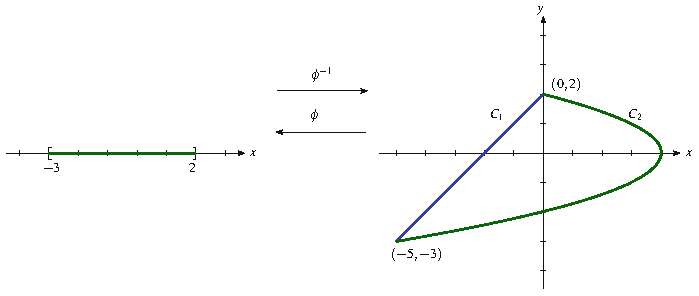
\includegraphics[width=0.945\linewidth]{images/vector/fig-7-16.pdf}
  \caption{映射 $\varphi^{-1}$ 把 $[-3,2]$ 送到曲线 $C_2$}
  \label{fig:7-16}
\end{figure}

\textbf{例二.} 在这个例子中，我们将做一些与例一中类似的事情. 回想在例一中，我们沿两条具有相同起点和终点的不同曲线 $C_1$ 和 $C_2$ 积分了一个 1-形式，并发现这两个积分是不同的，也就是说，积分依赖于所取的路径. 我们将使用一个不同的 1-形式来重复这一点. 这次我们积分的 1-形式将是一种特殊的 1-形式，它将是某个 0-形式的外微分.

我们将选择 $\mathbb{R}^2$ 上的 0-形式（函数）$f(x,y)=x^2y$. 对这个 0-形式取外微分，给出 1-形式
\[
df=\frac{\partial f}{\partial x}dx+\frac{\partial f}{\partial y}dy=2xy\,dx+x^2dy.
\]
这就是我们要积分的 1-形式. 我们将使用与例一中相同的路径和参数化. 这个过程本质上与前面的例子相同. 我们知道 $T^*\varphi^{-1}\cdot\bigl(2xydx+x^2dy\bigr)$ 是 $\mathbb{R}$ 上的 1-形式，所以它必然具有某个函数 $f(t)$ 决定的 $f(t)\,dt$ 的形式. 对曲线 $C_1$，我们求出
\begin{align*}
f(t)&=f(t)\,dt\bigl([1]\bigr)\\
&=T^*\varphi^{-1}\cdot\bigl(2xydx+x^2dy\bigr)\bigl([1]\bigr)\\
&=\bigl(2xydx+x^2dy\bigr)\binom{5}{5}\\
&=10xy+5x^2\\
&=10(5t-5)(5t-3)+5(5t-5)^2\\
&=5(75t^2-130t+55),
\end{align*}
于是我们有 $T^*\varphi^{-1}\cdot\bigl(2xydx+x^2dy\bigr)=5(75t^2-130t+55)\,dt$. 我们使用恒等式 $\int_C\alpha=\int_{\varphi(C)}T^*\varphi^{-1}\cdot\alpha$，得到
\begin{align*}
\int_{C_1}2xydx+x^2dy
&=\int_{\varphi(C_1)}T^*\varphi^{-1}\cdot\bigl(2xydx+x^2dy\bigr)\\
&=\int_{[0,1]}5(75t^2-130t+55)\,dt\\
&=75.
\end{align*}
现在我们沿路径 $C_2$ 取积分. 类似地我们求出
\begin{align*}
f(t)&=f(t)\,dt\bigl([1]\bigr)\\
&=T^*\varphi^{-1}\cdot\bigl(2xydx+x^2dy\bigr)\bigl([1]\bigr)\\
&=\bigl(2xydx+x^2dy\bigr)\binom{-2t}{1}\\
&=2xy(-2t)+x^2(1)\\
&=2(4-t^2)(t)(-2t)+(4-t^2)^2\\
&=5t^4-24t^2+16,
\end{align*}
于是我们有 $T^*\varphi^{-1}\cdot\bigl(2xydx+x^2dy\bigr)=\bigl(5t^4-24t^2+16\bigr)dt$. 积分是
\begin{align*}
\int_{C_2}2xydx+x^2dy
&=\int_{\varphi(C_2)}T^*\varphi^{-1}\cdot\bigl(2xydx+x^2dy\bigr)\\
&=\int_{[-3,2]}\bigl(5t^4-24t^2+16\bigr)dt\\
&=75.
\end{align*}
有趣的事情发生了. 当我们的 1-形式是某个 0-形式的外微分时，我们的积分结果似乎不依赖于所取的路径. 事实上，这普遍成立，并不仅仅在这个例子中成立. 我们将在后面更详细地考察这一点.

\textbf{例三.} 我们的下一个例子涉及在 $\mathbb{R}^3$ 中沿从点 $(2,0,0)$ 到点 $(3,4,5)$ 的直线路径 $C$ 积分 1-形式 $ydx+zdy+xdz$. 我们求这条路径的一个参数化 $\varphi^{-1}:\mathbb{R}\to\mathbb{R}^3$，由 $\varphi^{-1}(t)=\bigl(x(t),y(t),z(t)\bigr)=(2+t,4t,5t)$ 给出. 令 $R=[0,1]\subset\mathbb{R}$，我们有 $\varphi^{-1}(R)=\bigl\{(x,y,z)\,\bigl|\,x=2+t,\ y=4t,\ z=5t,\ 0\leq t\leq 1\bigr\}=C$. 这给出
\[
T_p\varphi^{-1}=\begin{bmatrix}\frac{\partial x}{\partial t}\\\frac{\partial y}{\partial t}\\\frac{\partial z}{\partial t}\end{bmatrix}_p=\begin{bmatrix}1\\4\\5\end{bmatrix}.
\]
显然，$T_p\varphi^{-1}$ 不依赖于基点 $p\in\mathbb{R}$. 和之前一样，我们知道 $T^*\varphi^{-1}\cdot(ydx+zdy+xdz)=f(t)\,dt$，其中 $f(t)$ 是某个函数，正是我们想求的. 计算过程与之前完全相同，
\begin{align*}
f(t)&=f(t)\,dt\bigl([1]\bigr)\\
&=T^*\varphi^{-1}\cdot(ydx+zdy+xdz)\bigl([1]\bigr)\\
&=(ydx+zdy+xdz)\bigl(T\varphi^{-1}\cdot[1]\bigr)\\
&=(ydx+zdy+xdz)\begin{bmatrix}1\\4\\5\end{bmatrix}\cdot[1]\\
&=ydx\begin{bmatrix}1\\4\\5\end{bmatrix}+zdy\begin{bmatrix}1\\4\\5\end{bmatrix}+xdz\begin{bmatrix}1\\4\\5\end{bmatrix}\\
&=y(1)+z(4)+x(5)\\
&=(4t)+4(5t)+5(2+t)\\
&=29t+10,
\end{align*}
于是我们有 $T^*\varphi^{-1}\cdot(ydx+zdy+xdz)=(29t+10)dt$. 利用 $\int_C\alpha=\int_{\varphi(C)}T^*\varphi^{-1}\cdot\alpha$，我们得到积分
\begin{align*}
\int_C(ydx+zdy+xdz)
&=\int_{\varphi(C)}T^*\varphi^{-1}\cdot(ydx+zdy+xdz)\\
&=\int_{[0,1]}(29t+10)\,dt\\
&=24\frac{1}{2}.
\end{align*}

\subsection{曲面积分}

现在我们将做几个在参数化二维曲面上积分 2-形式的例子.

\textbf{例一.} 我们将在单位球面的上半部分上积分 2-形式 $z^2dx\wedge dy$. 我们将使用由
\[
\varphi^{-1}(r,\theta)=\bigl(x(r,\theta),y(r,\theta),z(r,\theta)\bigr)=\Bigl(r\cos\theta,\ r\sin\theta,\ \sqrt{1-r^2}\Bigr)
\]
给出的参数化. 令 $R=\bigl\{(r,\theta)\,\bigl|\,0\leq r\leq 1,\ 0\leq\theta\leq 2\pi\bigr\}$，我们有 $\varphi^{-1}(R)$ 是单位球面的上半部分. 见图~\ref{fig:7-17}. 首先我们求 $T\varphi^{-1}$，
\begin{align*}
T\varphi^{-1}&=\begin{bmatrix}\frac{\partial x}{\partial r}&\frac{\partial x}{\partial\theta}\\\frac{\partial y}{\partial r}&\frac{\partial y}{\partial\theta}\\\frac{\partial z}{\partial r}&\frac{\partial z}{\partial\theta}\end{bmatrix}
=\begin{bmatrix}\frac{\partial(r\cos\theta)}{\partial r}&\frac{\partial(r\cos\theta)}{\partial\theta}\\\frac{\partial(r\sin\theta)}{\partial r}&\frac{\partial(r\sin\theta)}{\partial\theta}\\\frac{\partial\sqrt{1-r^2}}{\partial r}&\frac{\partial\sqrt{1-r^2}}{\partial\theta}\end{bmatrix}\\
&=\begin{bmatrix}\cos\theta&-r\sin\theta\\\sin\theta&r\cos\theta\\-\frac{r}{\sqrt{1-r^2}}&0\end{bmatrix}.
\end{align*}

\begin{figure}[htbp]
  \centering
  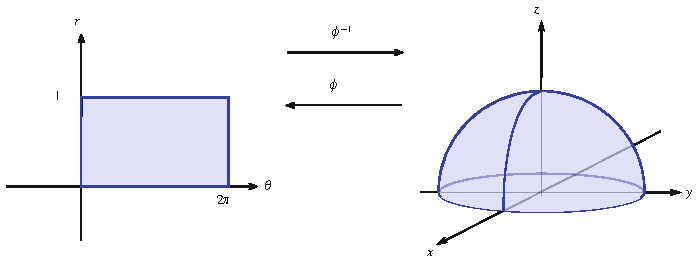
\includegraphics[width=0.957\linewidth]{images/vector/fig-7-17.pdf}
  \caption{映射 $\varphi^{-1}$ 把 $R=\bigl\{(r,\theta)\,\bigl|\,0\leq r\leq 1,\ 0\leq\theta\leq 2\pi\bigr\}$ 送到 $\mathbb{R}^3$ 中单位球面的顶部}
  \label{fig:7-17}
\end{figure}

现在我们要求 $T^*\varphi^{-1}\cdot\bigl(z^2dx\wedge dy\bigr)$. 我们知道这是 $\mathbb{R}^2$ 上的 2-形式，所以它必然具有某个函数 $g(r,\theta)$ 决定的 $g(r,\theta)\,dr\wedge d\theta$ 的形式. 我们的目标是求出这个函数. 注意
\[
g(r,\theta)\,dr\wedge d\theta\left(\binom{1}{0},\binom{0}{1}\right)=g(r,\theta)\begin{vmatrix}1&0\\0&1\end{vmatrix}=g(r,\theta).
\]
因此，
\begin{align*}
g(r,\theta)&=g(r,\theta)\,dr\wedge d\theta\left(\binom{1}{0},\binom{0}{1}\right)\\
&=T^*\varphi^{-1}\cdot\bigl(z^2dx\wedge dy\bigr)\left(\binom{1}{0},\binom{0}{1}\right)\\
&=z^2dx\wedge dy\left(T\varphi^{-1}\cdot\binom{1}{0},T\varphi^{-1}\cdot\binom{0}{1}\right)\\
&=z^2dx\wedge dy\left(\begin{bmatrix}\cos\theta\\\sin\theta\\-\frac{r}{\sqrt{1-r^2}}\end{bmatrix},\begin{bmatrix}-r\sin\theta\\r\cos\theta\\0\end{bmatrix}\right)\\
&=z^2\begin{vmatrix}\cos\theta&-r\sin\theta\\\sin\theta&r\cos\theta\end{vmatrix}\\
&=z^2r\\
&=\Bigl(\sqrt{1-r^2}\Bigr)^2r\\
&=r-r^3,
\end{align*}
\[
\Rightarrow\ T^*\varphi^{-1}\cdot\bigl(z^2dx\wedge dy\bigr)=\bigl(r-r^3\bigr)dr\wedge d\theta.
\]
利用恒等式 $\int_R\alpha=\int_{\varphi(R)}T^*\varphi^{-1}\cdot\alpha$，我们有
\begin{align*}
\int_R z^2dx\wedge dy
&=\int_{\varphi(R)}\bigl(r-r^3\bigr)dr\wedge d\theta\\
&=\int_0^{2\pi}\int_0^1\bigl(r-r^3\bigr)dr\,d\theta\\
&=\int_0^{2\pi}\left.\left(\frac{r^2}{2}-\frac{r^4}{4}\right)\right|_0^1d\theta\\
&=\int_0^{2\pi}\frac{1}{4}\,d\theta\\
&=\frac{\pi}{2}.
\end{align*}

\textbf{例二.} 现在我们将使用下面三种参数化，在单位球面的上半部分上积分 2-形式 $\alpha=\frac{1}{x}dy\wedge dz-\frac{1}{y}dx\wedge dz$. 我们将完成第一个参数化，把另外两个留作练习.
\begin{enumerate}
  \item[(a)] $(r,\theta)\mapsto\Bigl(r\cos\theta,\ r\sin\theta,\ \sqrt{1-r^2}\Bigr)$，$0\leq\theta\leq 2\pi$，$0\leq r\leq 1$
  \item[(b)] $(\theta,\varphi)\mapsto(\sin\varphi\cos\theta,\ \sin\varphi\sin\theta,\ \cos\varphi)$，$0\leq\theta\leq 2\pi$，$0\leq\varphi\leq\frac{\pi}{2}$
  \item[(c)] $(x,y)\mapsto\Bigl(x,\ y,\ \sqrt{1-x^2-y^2}\Bigr)$，$x^2+y^2\leq 1$
\end{enumerate}
我们应该预期，无论使用哪种参数化，都会得到相同的答案. 我们现在进行第一个参数化，它仿照例一，只不过我们有
\[
g(r,\theta)\,dr\wedge d\theta=T^*\varphi^{-1}\cdot\left(\frac{1}{x}dy\wedge dz-\frac{1}{y}dx\wedge dz\right)\longmapsto\frac{1}{x}dy\wedge dz-\frac{1}{y}dx\wedge dz.
\]
我们想求 $g(r,\theta)$，令 $e_1$ 和 $e_2$ 分别是 $r$ 方向和 $\theta$ 方向的单位向量，于是我们有
\begin{align*}
g(r,\theta)&=g(r,\theta)\,dr\wedge d\theta(e_1,e_2)\\
&=T^*\varphi^{-1}\cdot\left(\frac{1}{x}dy\wedge dz-\frac{1}{y}dx\wedge dz\right)(e_1,e_2)\\
&=\left(\frac{1}{x}dy\wedge dz-\frac{1}{y}dx\wedge dz\right)(T\varphi\cdot e_1,T\varphi\cdot e_2)\\
&=\left(\frac{1}{x}dy\wedge dz-\frac{1}{y}dx\wedge dz\right)\left(\begin{bmatrix}\cos\theta\\\sin\theta\\-\frac{r}{\sqrt{1-r^2}}\end{bmatrix},\begin{bmatrix}-r\sin\theta\\r\cos\theta\\0\end{bmatrix}\right)\\
&=\frac{1}{x}dy\wedge dz\left(\begin{bmatrix}\cos\theta\\\sin\theta\\-\frac{r}{\sqrt{1-r^2}}\end{bmatrix},\begin{bmatrix}-r\sin\theta\\r\cos\theta\\0\end{bmatrix}\right)-\frac{1}{y}dx\wedge dz\left(\begin{bmatrix}\cos\theta\\\sin\theta\\-\frac{r}{\sqrt{1-r^2}}\end{bmatrix},\begin{bmatrix}-r\sin\theta\\r\cos\theta\\0\end{bmatrix}\right)\\
&=\frac{1}{x}\begin{vmatrix}\sin\theta&r\cos\theta\\-\frac{r}{\sqrt{1-r^2}}&0\end{vmatrix}-\frac{1}{y}\begin{vmatrix}\cos\theta&-r\sin\theta\\-\frac{r}{\sqrt{1-r^2}}&0\end{vmatrix}\\
&=\frac{1}{x}\frac{r^2\cos\theta}{\sqrt{1-r^2}}-\frac{1}{y}\frac{-r^2\sin\theta}{\sqrt{1-r^2}}\\
&=\frac{1}{r\cos\theta}\frac{r^2\cos\theta}{\sqrt{1-r^2}}-\frac{1}{r\sin\theta}\frac{-r^2\sin\theta}{\sqrt{1-r^2}}\\
&=\frac{2r}{\sqrt{1-r^2}},
\end{align*}
\[
\Rightarrow\ T^*\varphi^{-1}\cdot\left(\frac{1}{x}dy\wedge dz-\frac{1}{y}dx\wedge dz\right)=\frac{2r}{\sqrt{1-r^2}}dr\wedge d\theta.
\]
现在我们用恒等式 $\int_R\alpha=\int_{\varphi(R)}T^*\varphi^{-1}\cdot\alpha$ 来取积分，
\begin{align*}
\int_R\frac{1}{x}dy\wedge dz-\frac{1}{y}dx\wedge dz
&=\int_{\varphi(R)}\frac{2r}{\sqrt{1-r^2}}dr\wedge d\theta\\
&=\int_0^{2\pi}\int_0^1\frac{2r}{\sqrt{1-r^2}}dr\,d\theta\\
&=2\int_0^{2\pi}d\theta\cdot\int_0^1\frac{r}{\sqrt{1-r^2}}dr\\
&=2\cdot 2\pi\cdot\left[-\sqrt{1-r^2}\right]_0^1\\
&=4\pi.
\end{align*}

\begin{question}\label{q:7-13}
用第二种和第三种参数化求积分，完成这个例子.
\end{question}

\section{小结、参考文献与问题}

\subsection{小结}

如果求积分 $\int_R f(x_1,x_2,\ldots,x_n)\,dx_1dx_2\cdots dx_n$ 是困难的，但通过做变量替换
\[
\mathbb{R}^n_{x_1x_2\cdots x_n}\xrightarrow{\ \varphi\ }\mathbb{R}^n_{\varphi_1\varphi_2\cdots\varphi_n},\qquad(x_1,x_2,\ldots,x_n)\longmapsto(\varphi_1,\varphi_2,\ldots,\varphi_n)
\]
它会变得容易，那么就可以使用变量替换公式
\[
\begin{aligned}
\text{变量替换公式}\qquad \int_R f(x_1,\ldots,x_n)\,dx_1\wedge\cdots\wedge dx_n
&=\int_{\varphi(R)}f\circ\varphi^{-1}(\varphi_1,\ldots,\varphi_n)\,T^*\varphi^{-1}\\
&\quad\cdot\bigl(dx_1\wedge\cdots\wedge dx_n\bigr).
\end{aligned}
\]
左边在 $x_1\cdots x_n$-坐标中进行，我们在区域 $R$ 上用与 $x_1\cdots x_n$-坐标相联系的体积形式 $dx_1\wedge\cdots\wedge dx_n$ 积分函数 $f(x_1,\ldots,x_n)$. 在右边，函数 $f\circ\varphi^{-1}:\mathbb{R}^n\to\mathbb{R}$ 是变量 $\varphi_1,\varphi_2,\ldots,\varphi_n$ 的函数. 我们在 $\mathbb{R}^n_{\varphi_1\varphi_2\cdots\varphi_n}$ 中积分的区域是像 $\varphi(R)$. 最后，右边的形式是 $T^*\varphi^{-1}\cdot\bigl(dx_1\wedge\cdots\wedge dx_n\bigr)$，即面积形式 $dx_1\wedge\cdots\wedge dx_n$ 由 $\varphi^{-1}$ 的拉回，而不是面积形式 $d\varphi_1\wedge\cdots\wedge d\varphi_n$. 这恰好给出了你在多元微积分中使用极坐标、柱坐标和球坐标做变量替换时用到的东西.

我们可以在曲线上积分 1-形式，在曲面上积分 2-形式，在三维空间中积分 3-形式，等等. 只要在一个 $n$ 维流形上有一个 $n$-形式，我们就可以对它积分. 给定流形 $\Sigma_k\subset\mathbb{R}^n$（$k<n$）的一个参数化，即一个可逆映射 $\varphi^{-1}:U\subset\mathbb{R}^k\to\Sigma_k\subset\mathbb{R}^n$，我们可以把 $k$-形式拉回到 $U\subset\mathbb{R}^k$ 并在那里积分，从而在 $\Sigma_k$ 上积分 $k$-形式. 在这种情况下，我们想使用的变量替换公式的版本是
\[
\text{$k$ 维参数化曲面 $\Sigma_k$ 上 $k$-形式的积分}\qquad\int_{\Sigma_k}\alpha=\int_{\varphi(\Sigma_k)}T^*\varphi^{-1}\cdot\alpha.
\]
当 $k=1$ 时，我们得到一条曲线，经常写 $\Sigma_1=C$；当 $k=2$ 时，我们得到一个曲面，经常写 $\Sigma_2=S$；当 $k=3$ 时，我们得到一个体积，经常写 $\Sigma_3=V$.

\subsection{参考文献与进一步阅读}

Riemann 和与变量替换几乎在每一本微积分或入门分析书中都会引入并讨论，而且常常不惜篇幅，例如见 Steward~\cite{ref43}、Hubbard 与 Hubbard~\cite{ref27}，或 Marsden 与 Hoffman~\cite{ref31}. 然而，在本章中，我们大体上遵循了 Bachman~\cite{ref04} 的讲述，因为它直接涉及微分形式的情形. 关于同一材料的更偏理论性的导引，另见 Watschap~\cite{ref47} 或 Renteln~\cite{ref37}.

\subsection{问题}

\begin{question}\label{q:7-14}
设 $C$ 是 $\mathbb{R}^3$ 中由 $\gamma(t)=\bigl(2t+1,\ t^2,\ t^3\bigr)$（$1\leq t\leq 3$）参数化的定向曲线，设 $\alpha=(3x-1)^2dx+5dy+2dz$ 是 $\mathbb{R}^3$ 上的 1-形式. 求 $\int_C\alpha$.
\end{question}

\begin{question}\label{q:7-15}
设 $C$ 是 $\mathbb{R}^3$ 中由 $\gamma(t)=\bigl(1-t^2,\ t^3-t,\ 0\bigr)$（$0\leq t\leq 2$）参数化的定向曲线. 注意曲线 $C$ 位于 $\mathbb{R}^2\subset\mathbb{R}^3$ 中. 设 $\alpha=-5xy\,dx+dz$ 是 $\mathbb{R}^3$ 上的 1-形式. 求 $\int_C\alpha$.
\end{question}

\begin{question}\label{q:7-16}
设 $C$ 是 $\mathbb{R}^2$ 中由 $\gamma(t)=\bigl(t^2,\ 2t+1\bigr)$（$1\leq t\leq 2$）参数化的曲线，设 $\alpha=4x\,dx+ydy$ 是 $\mathbb{R}^2$ 上的 1-形式. 求 $\int_C\alpha$.
\end{question}

\begin{question}\label{q:7-17}
设 $C$ 是平面 $\mathbb{R}^2$ 中作为函数 $y=1+x^2$（$-1\leq x\leq 1$）图像的曲线，按 $x$ 增大的方向定向，设 $\alpha=y\,dx+x\,dy$ 是平面上的 1-形式. 求 $\int_C\alpha$. （虽然并非必要，也可以把曲线 $C$ 参数化为 $\gamma(t)=(t,1+t^2)$，$-1\leq t\leq 1$.）
\end{question}

\begin{question}\label{q:7-18}
设 $C_1$ 和 $C_2$ 是平面 $\mathbb{R}^2$ 中的曲线，分别由 $\gamma_1(t)=(t-1,2t-1)$（$1\leq t\leq 2$）和 $\gamma_2(u)=(2-u,5-2u)$（$1\leq u\leq 2$）参数化. 设 $\alpha=y\,dx$ 是 $\mathbb{R}^2$ 上的 1-形式. 求 $\int_{C_1}\alpha$ 和 $\int_{C_2}\alpha$. 比较这两个答案，并解释它们之间的关系.
\end{question}

\begin{question}\label{q:7-19}
设 $C$ 是 $\mathbb{R}^2$ 中由 $\gamma(\theta)=\bigl(\cos(\theta),\sin(\theta)\bigr)$（$0\leq\theta\leq 2\pi$）参数化的单位圆. 设
\[
\alpha_1=\frac{-y}{x^2+y^2}dx+\frac{x}{x^2+y^2}dy,\qquad
\alpha_2=\frac{x}{x^2+y^2}dx+\frac{y}{x^2+y^2}dy
\]
是 $\mathbb{R}^2$ 上的 1-形式. 求 $\int_C\alpha_1$ 和 $\int_C\alpha_2$. 注意，可以把 $\alpha_1$ 写成 $\alpha_1=-\sin(\theta)\,dx+\cos(\theta)\,dy$，把 $\alpha_2$ 写成 $\alpha_2=\cos(\theta)\,dx+\sin(\theta)\,dy$.
\end{question}

\begin{question}\label{q:7-20}
设 $C$ 是 $\mathbb{R}^2$ 中的一条曲线. 曲线 $C$ 既可以由 $\gamma_1(t)=\bigl(t,\sqrt{1+t^2}\bigr)$（$-1\leq t\leq 1$）参数化，也可以由 $\gamma_2(\theta)=\bigl(\tan(\theta),\sec(\theta)\bigr)$（$-\frac{\pi}{4}\leq\theta\leq\frac{\pi}{4}$）参数化. 设 $\alpha=y^2\,dx$ 是 $\mathbb{R}^2$ 上的 1-形式. 用 $C$ 的每一种参数化求 $\int_C\alpha$.
\end{question}

\begin{question}\label{q:7-21}
设 $C$ 是 $\mathbb{R}^2$ 中的一条曲线. 曲线 $C$ 可以参数化为 $\gamma_1(t)=\bigl(t,t^2\bigr)$（$-2\leq t\leq 2$），或者 $\gamma_2(u)=\bigl(u^3+u,\ u^6+2u^4+u^2\bigr)$（$-1\leq u\leq 1$），或者 $\gamma_3(\theta)=\bigl(4\sin(\theta),\ 16\sin^2(\theta)\bigr)$（$-\frac{\pi}{6}\leq\theta\leq\frac{\pi}{6}$）. 如果 $\alpha=5xy\,dy$ 是 $\mathbb{R}^2$ 上的 1-形式，用全部三种参数化求 $\int_C\alpha$.
\end{question}

\begin{question}\label{q:7-22}
考虑 $\mathbb{R}^3$ 中由 $\varphi(x,y)=\bigl(x,\ y,\ x^3+xy^2\bigr)$（$1\leq x\leq 3,\ 1\leq y\leq 2$）参数化的曲面 $S$，以及 $\mathbb{R}^3$ 上的 2-形式 $\beta=2xyz\,dx\wedge dy+6(2x^3-y^3)\,dy\wedge dz+z\,dz\wedge dx$. 求 $\int_S\beta$.
\end{question}

\begin{question}\label{q:7-23}
设 $U$ 是单位圆盘的上半部分，$U=\bigl\{(x,y)\,\bigl|\,-1\leq x\leq 1,\ 0\leq y\leq\sqrt{1-x^2}\bigr\}$. 设 $\mathbb{R}^3$ 中的曲面 $S$ 由 $\varphi(x,y)=\bigl(x,\ y,\ x^2+y^2\bigr)$（$(x,y)\in U$）参数化，设 $\beta=6y\,dx\wedge dy$ 是 $\mathbb{R}^3$ 上的 2-形式. 求 $\int_S\beta$.
\end{question}

\begin{question}\label{q:7-24}
设 $U$ 是 $\mathbb{R}^2$ 中的三角形区域 $U=\bigl\{(u,v)\,\bigl|\,0\leq u\leq 1,\ 0\leq v\leq 1-u\bigr\}$. 设 $\mathbb{R}^3$ 中的曲面 $S$ 由 $\varphi(u,v)=\bigl(u-v,\ uv,\ u^2+(v+1)^2\bigr)$（$(u,v)\in U$）参数化，设 $\beta=-(1+x^2)\,dx\wedge dy+dy\wedge dz$. 求 $\int_S\beta$.
\end{question}

\begin{question}\label{q:7-25}
设 $U=\bigl\{(u,v)\,\bigl|\,-1\leq u\leq 1,\ -2\leq v\leq 2\bigr\}\subset\mathbb{R}^2$，设 $\mathbb{R}^3$ 中的曲面 $S$ 由 $\varphi(u,v)=\bigl(u,\ v,\ u^3+3uv^2\bigr)$（$(u,v)\in U$）参数化. 设 $\beta=-dy\wedge dz+dz\wedge dx$. 求 $\int_S\beta$.
\end{question}

\begin{question}\label{q:7-26}
设 $U=\bigl\{(u,v)\,\bigl|\,0\leq u\leq 1,\ 0\leq v\leq 2\bigr\}\subset\mathbb{R}^2$，设 $\mathbb{R}^3$ 中的曲面 $S$ 由 $\varphi(u,v)=\bigl(u,\ v,\ u^2+v^3\bigr)$（$(u,v)\in U$）参数化. 设 $\beta=31x^2y^3\,dx\wedge dy+5xz\,dy\wedge dz+7yz\,dz\wedge dx$. 求 $\int_S\beta$.
\end{question}

\begin{question}\label{q:7-27}
设 $U=\bigl\{(u,v)\,\bigl|\,u^2+v^2\leq 9\bigr\}\subset\mathbb{R}^2$，设 $\mathbb{R}^3$ 中的曲面 $S$ 由 $\varphi(u,v)=\bigl(u,\ v,\ 7+(u^2+v^2)\bigr)$（$(u,v)\in U$）参数化. 设 $\beta=z^2dx\wedge dy$. 求 $\int_S\beta$.
\end{question}

\begin{question}\label{q:7-28}
设 $U=\bigl\{(u,v)\,\bigl|\,u^2+v^2\leq 9\bigr\}\subset\mathbb{R}^2$，设 $\mathbb{R}^3$ 中的曲面 $S$ 由 $\varphi(u,v)=\bigl(u,\ v,\ 25-(u^2+v^2)\bigr)$（$(u,v)\in U$）参数化. 设 $\beta=z^2dx\wedge dy$. 求 $\int_S\beta$.
\end{question}

\begin{question}\label{q:7-29}
设 $U=\bigl\{(u,v)\,\bigl|\,0\leq u\leq 1,\ 0\leq v\leq 2\bigr\}\subset\mathbb{R}^2$，设 $\mathbb{R}^3$ 中的曲面 $S$ 由 $\varphi(u,v)=\bigl(u+v,\ u-v^2,\ uv\bigr)$（$(u,v)\in U$）参数化. 设 $\beta=6z\,dz\wedge dx$. 求 $\int_S\beta$.
\end{question}

\begin{question}\label{q:7-30}
设 $U=\bigl\{(u,v)\,\bigl|\,1\leq u\leq 2,\ 0\leq v\leq 2\pi\bigr\}\subset\mathbb{R}^2$，设 $\mathbb{R}^3$ 中的曲面 $S$ 由 $\varphi(u,v)=\bigl(u^3\cos(v),\ u^3\sin(v),\ u^2\bigr)$（$(u,v)\in U$）参数化. 设 $\beta=2z\,dx\wedge dy-x\,dy\wedge dz-y\,dz\wedge dx$. 求 $\int_S\beta$.
\end{question}

\begin{question}\label{q:7-31}
设 $\alpha=xy\,dx\wedge dy$ 是 $\mathbb{R}^2$ 上的 2-形式，设 $D$ 是以原点为圆心、半径为 3 的圆盘. 用极坐标变量替换求 $\int_D\alpha$.
\end{question}

\begin{question}\label{q:7-32}
设 $\alpha=(3x+4y^2)\,dx\wedge dy$ 是 $\mathbb{R}^2$ 上的 2-形式，设 $R$ 是由圆 $x^2+y^2=1$ 和 $x^2+y^2=9$ 围成的上半平面中的区域. 用极坐标变量替换求 $\int_R\alpha$.
\end{question}

\begin{question}\label{q:7-33}
设 $\alpha=(x+y)\,dx\wedge dy$ 是 $\mathbb{R}^2$ 上的 2-形式，设 $R$ 是 $y$ 轴左侧、由圆 $x^2+y^2=1$ 和 $x^2+y^2=9$ 围成的区域. 用极坐标变量替换求 $\int_R\alpha$.
\end{question}

\begin{question}\label{q:7-34}
设 $\alpha=\cos(x^2+y^2)\,dx\wedge dy$ 是 $\mathbb{R}^2$ 上的 2-形式，设 $R$ 是 $x$ 轴上方、圆 $x^2+y^2=4$ 内部的区域. 用极坐标变量替换求 $\int_R\alpha$.
\end{question}

\begin{question}\label{q:7-35}
设 $V\subset\mathbb{R}^3$ 是位于圆柱面 $x^2+y^2=1$ 内部、平面 $z=0$ 与 $z=5$ 之间的区域，设 $\beta=x\,dx\wedge dy\wedge dz$ 是 $\mathbb{R}^3$ 上的 3-形式. 用柱坐标变量替换求 $\int_V\beta$.
\end{question}

\begin{question}\label{q:7-36}
设 $V\subset\mathbb{R}^3$ 是位于圆柱面 $x^2+y^2=25$ 内部、平面 $z=-5$ 与 $z=5$ 之间的区域，设 $\beta=\sqrt{x^2+y^2}\,dx\wedge dy\wedge dz$ 是 $\mathbb{R}^3$ 上的 3-形式. 用柱坐标变量替换求 $\int_V\beta$.
\end{question}

\begin{question}\label{q:7-37}
设 $V=\Bigl\{(x,y,z)\,\Bigl|\,-2\leq x\leq 2,\ -\sqrt{4-x^2}\leq y\leq\sqrt{4-x^2},\ \sqrt{x^2+y^2}\leq z\leq 2\Bigr\}\subset\mathbb{R}^3$，设 $\beta=(x^2+y^2)\,dx\wedge dy\wedge dz$ 是 $\mathbb{R}^3$ 上的 3-形式. 用柱坐标变量替换求 $\int_V\beta$.
\end{question}

\begin{question}\label{q:7-38}
设 $V\subset\mathbb{R}^3$ 是位于圆柱面 $x^2+y^2=1$ 与 $x^2+y^2=4$ 之间、平面 $z=0$ 与 $z=x+2$ 之间的区域，设 $\beta=y\,dx\wedge dy\wedge dz$ 是 $\mathbb{R}^3$ 上的 3-形式. 用柱坐标变量替换求 $\int_V\beta$.
\end{question}

\begin{question}\label{q:7-39}
设 $V=\bigl\{(x,y,z)\,\bigl|\,x^2+y^2+z^2\leq 1\bigr\}$，即 $\mathbb{R}^3$ 中的单位球，设 $\beta=e^{(x^2+y^2+z^2)^{3/2}}dx\wedge dy\wedge dz$ 是 $\mathbb{R}^3$ 上的 3-形式. 用球坐标变量替换求 $\int_V\beta$.
\end{question}

\begin{question}\label{q:7-40}
设 $V=\bigl\{(x,y,z)\,\bigl|\,x^2+y^2+z^2\leq 1\bigr\}$，即 $\mathbb{R}^3$ 中的单位球，设 $\beta=e^{(x^2+y^2+z^2)^{3/2}}dx\wedge dy\wedge dz$ 是 $\mathbb{R}^3$ 上的 3-形式. 用球坐标变量替换求 $\int_V\beta$.
\end{question}

\begin{question}\label{q:7-41}
设 $V=\bigl\{(x,y,z)\,\bigl|\,x^2+y^2+z^2\leq 5\bigr\}$，即以原点为球心、半径为 $\sqrt{5}$ 的球，设 $\beta=(x^2+y^2+z^2)^2\,dx\wedge dy\wedge dz$ 是 $\mathbb{R}^3$ 上的 3-形式. 用球坐标变量替换求 $\int_V\beta$.
\end{question}

\begin{question}\label{q:7-42}
求 $\mathbb{R}^3$ 中圆锥面 $z=\sqrt{x^2+y^2}$ 上方、球面 $x^2+y^2+z^2=z$ 下方的区域的体积. 这意味着我们要积分的 3-形式是体积形式 $dx\wedge dy\wedge dz$. 使用球坐标变量替换.
\end{question}

---

% 第 8 章 Poincaré 引理
\chapter{Poincaré 引理}

简而言之，Poincaré 引理如下.
\begin{theorem}[Poincaré 引理]\label{thm:8-1}
$\mathbb{R}^n$ 上的每个闭形式都是恰当的.
\end{theorem}
第 1 节详细介绍 Poincaré 引理及其含义. 严格地说，整个空间 $\mathbb{R}^n$ 并不是必需的. 证明对任何可缩为一点的星形区域都成立，但既然这不在证明中起本质作用，为了尽可能清晰，我们将简单地假设流形都是某个 $n\geq0$ 的 $\mathbb{R}^n$.

Poincaré 引理的证明基于归纳法. 如果你还没有上过数学证明课，我们将放慢速度、仔细地逐步进行，尽量把每一步解释清楚. 虽然这不是一门证明技巧课，但希望学完本章后你能对归纳证明是什么样子有一个好的认识. 第 2 节讲述所谓归纳证明的基础情形，第 3 节讲述证明的一般情形.

Poincaré 引理在一个称为 \newterm{de-rham-cohomology}{de Rham 上同调}{de Rham cohomology} 的数学分支中起着重要作用，该分支在附录 B 中简要介绍.

\section{Poincaré 引理导引}

Poincaré 引理断言 $\mathbb{R}^n$ 上的每个闭形式都是恰当的. 若 $d\alpha=0$，则微分形式 $\alpha$ 称为\newterm{closed}{闭的}{closed}. 若存在另一个微分形式 $\beta$ 使得 $\alpha=d\beta$，则微分形式 $\alpha$ 称为\newterm{exact}{恰当的}{exact}. 显然，若 $\alpha$ 是恰当的 $k$-形式，则 $\beta$ 必是 $(k-1)$-形式. 因此，Poincaré 引理还可以表述为：若 $\alpha$ 是 $\mathbb{R}^n$ 上满足 $d\alpha=0$ 的 $k$-形式，则存在某个 $(k-1)$-形式 $\beta$ 使得 $\alpha=d\beta$.

我们从考察某个流形 $M$ 上的恰当形式开始. 若一个 $k$-形式等于某个 $(k-1)$-形式的外微分，则称它是恰当的. 因此，所有恰当 $k$-形式的集合正是所有 $d\alpha$（其中 $\alpha$ 是 $(k-1)$-形式）的集合. 另一种说法是：恰当形式的集合是 $d:\Omega^{k-1}(M)\to\Omega^k(M)$ 在 $\Omega^{k-1}(M)$ 下的像. 图 \ref{fig:8-1} 用维恩图式的图解给出了映射 $d:\Omega^{k-1}(M)\to\Omega^k(M)$，以描绘恰当 $k$-形式.

\begin{figure}[htbp]
  \centering
  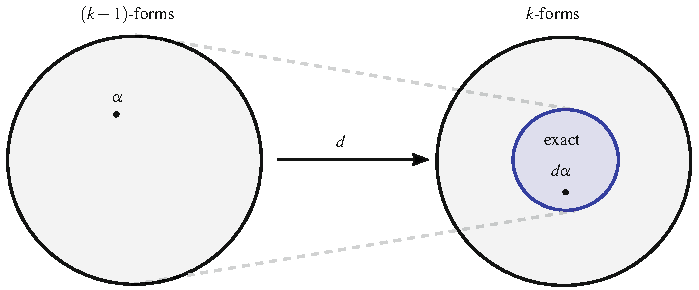
\includegraphics[width=0.829\linewidth]{images/vector/fig-8-1.pdf}
  \caption{用维恩图式图解说明的映射 $d:\Omega^{k-1}(M)\to\Omega^k(M)$. 恰当的 $k$-形式是 $\Omega^{k-1}(M)$ 在 $d$ 下的像}
  \label{fig:8-1}
\end{figure}

若 $M$ 上的 $k$-形式的外微分为零，即它等于零 $(k+1)$-形式，则称该 $k$-形式是闭的. 零 $(k+1)$-形式是每个把任意一组 $k+1$ 个向量都送到零的形式，它不应与零形式（即函数）混淆. 我们通常把任意点 $p$ 处的零 $k$-形式简单记为 $0$. 因此，所有闭 $k$-形式的集合就是满足 $d\alpha=0$ 的那些 $k$-形式 $\alpha$ 的集合. 另一种说法是：闭 $k$-形式的集合是零 $(k+1)$-形式在映射 $d:\Omega^k(M)\to\Omega^{k+1}(M)$ 下的原像. 图 \ref{fig:8-2} 用维恩图式给出了闭 $k$-形式的图像.

\begin{figure}[htbp]
  \centering
  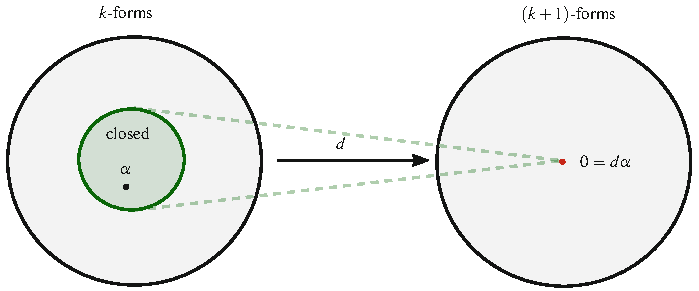
\includegraphics[width=0.829\linewidth]{images/vector/fig-8-2.pdf}
  \caption{用维恩图式图解说明的映射 $d:\Omega^k(M)\to\Omega^{k+1}(M)$. 闭的 $k$-形式是零 $(k+1)$-形式 $0$ 在 $d$ 下的原像}
  \label{fig:8-2}
\end{figure}

现在问题变成：闭 $k$-形式与恰当 $k$-形式之间有什么关系. 第一个猜测可能会沿着图 \ref{fig:8-3} 的思路，其中显示了若干种不同的可能性：
\begin{itemize}
  \item 恰当形式是闭形式的子集.
  \item 恰当形式与闭形式相同.
  \item 闭形式是恰当形式的子集.
  \item 闭形式与恰当形式互斥.
  \item 闭形式与恰当形式互不为对方的子集，但也不互斥.
\end{itemize}

\begin{figure}[htbp]
  \centering
  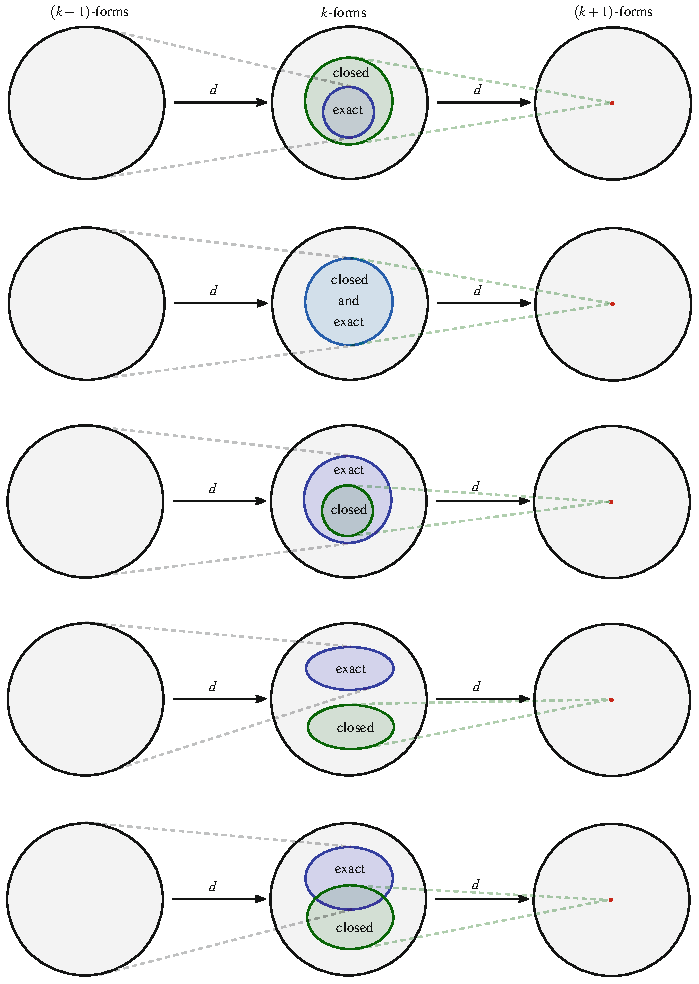
\includegraphics[width=0.885\linewidth]{images/vector/fig-8-3.pdf}
  \caption{闭 $k$-形式与恰当 $k$-形式之间可能存在的各种关系}
  \label{fig:8-3}
\end{figure}

然而，稍加思考几乎立刻就能排除最后三种可能性. 我们要做的只是认识到两个事实. 第一，每个恰当 $k$-形式都是某个 $(k-1)$-形式 $\alpha$ 的 $d\alpha$；第二，无论形式是什么，我们都有 $dd\alpha=0$. 这意味着每个恰当形式也是闭形式，从而排除了图 \ref{fig:8-3} 中的最后三种可能性. 剩下前两种可能性，即图 \ref{fig:8-4}.

\begin{figure}[htbp]
  \centering
  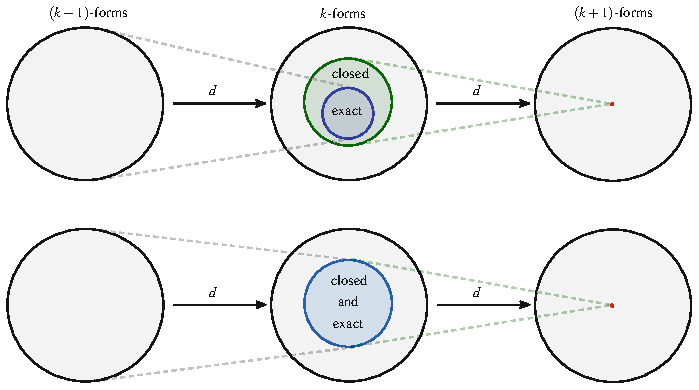
\includegraphics[width=0.907\linewidth]{images/vector/fig-8-4.pdf}
  \caption{恰当的 $k$-形式是闭 $k$-形式的子集（上方），还是与闭 $k$-形式相同（下方）？答案取决于流形 $M$}
  \label{fig:8-4}
\end{figure}

那么，图 \ref{fig:8-4} 中的两种可能性到底是哪一种呢？恰当形式是闭形式的子集，还是恰当形式与闭形式相同？结果表明，这个问题的答案取决于形式所在流形 $M$ 是什么. Poincaré 引理告诉我们，当流形是任意数 $n$ 的 $\mathbb{R}^n$ 时，恰当形式与闭形式相同. 但如果流形不是 $\mathbb{R}^n$，则情况未必如此. 称为 de Rham 上同调的数学分支考察 $M$ 上闭形式的集合与 $M$ 上恰当形式的集合相差多少，并利用这一信息来弄清底层流形 $M$ 的某些性质.

图 \ref{fig:8-5} 是一个交换图，展示了 $\mathbb{R}^n$ 上所有形式的空间，它向右和向下延伸到无穷. 显然，外微分给出映射序列
\[
\Omega^0(\mathbb{R}^n)\xrightarrow{\;d\;}\Omega^1(\mathbb{R}^n)\xrightarrow{\;d\;}\Omega^2(\mathbb{R}^n)\xrightarrow{\;d\;}\Omega^3(\mathbb{R}^n)\xrightarrow{\;d\;}\cdots
\]
对 $n=0,1,2,\ldots$ 的流形 $\mathbb{R}^n$ 成立. 映射 $K$ 是证明 Poincaré 引理所需的，将在下一节解释. 这给出交换图中的列. 映射
\[
Z:\Omega^k(\mathbb{R}^n)\to\Omega^k(\mathbb{R}^{n-1}),\qquad
C:\Omega^k(\mathbb{R}^n)\to\Omega^k(\mathbb{R}^{n+1}),
\]
其中 $k=1,2,\ldots$、$n=0,1,2,\ldots$，是我们证明 Poincaré 引理要用到的映射，它们也将在下一节引入. 在 Poincaré 引理的证明过程中，我们会反复参考这个交换图. 我们的目标是证明对 $n>0$ 的 $\mathbb{R}^n$ 上任意 $k>0$ 的闭 $k$-形式 $\alpha$ 都是恰当的. 换言之，我们要证明对每个满足 $d\alpha=0$ 的 $\alpha\in\Omega^k(\mathbb{R}^n)$，都存在 $\beta\in\Omega^{k-1}(\mathbb{R}^n)$ 使得 $\alpha=d\beta$. 实际上，我们不会显式地求出这个 $\beta$，而是对 $n$ 使用归纳法. 也就是说，如果我们知道它对 $\mathbb{R}^n$ 上的 $k$-形式成立，那么我们就能证明它对 $\mathbb{R}^{n+1}$ 成立. 图 \ref{fig:8-6} 给出了图 \ref{fig:8-5} 中交换图的列的维恩图式表示.

\begin{figure}[htbp]
  \centering
  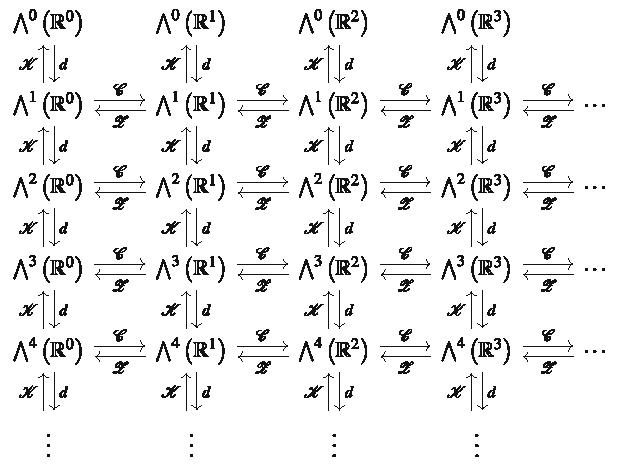
\includegraphics[width=0.856\linewidth]{images/vector/fig-8-5.pdf}
  \caption{有助于理解 Poincaré 引理证明的交换图}
  \label{fig:8-5}
\end{figure}

\begin{figure}[htbp]
  \centering
  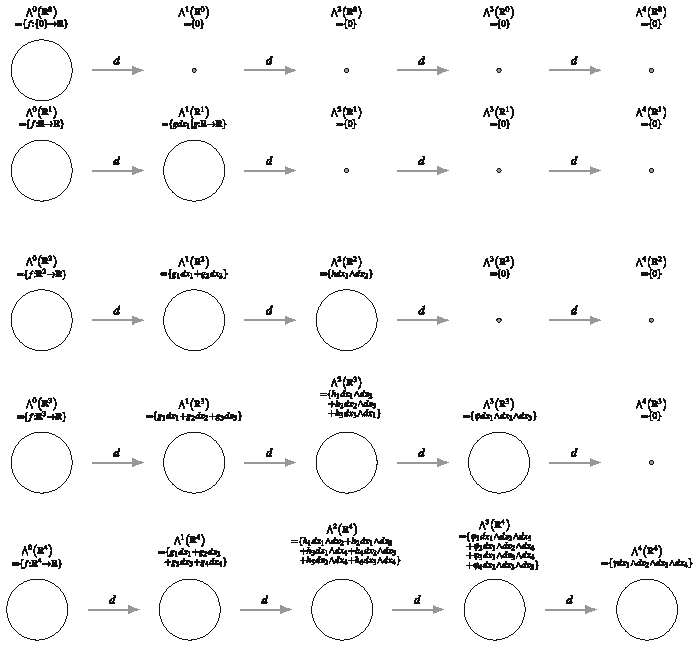
\includegraphics[width=0.960\linewidth]{images/vector/fig-8-6.pdf}
  \caption{这里把图 \ref{fig:8-5} 的列用维恩图式画成行. 归纳假设的基础情形是图 \ref{fig:8-5} 的第一列，此处画成最上一行. 图 \ref{fig:8-5} 的交换图中与我们的中等难度例子相关联的那一列画成第四行}
  \label{fig:8-6}
\end{figure}

\section{基础情形与一个简单例子}

首先我们回忆，$\mathbb{R}^n$ 上的零形式 $\alpha$ 正是 $\mathbb{R}^n$ 上的实值函数. $\mathbb{R}^n$ 上的零形式记为 $\Omega^0(\mathbb{R}^n)$，即图 \ref{fig:8-5} 的最上一行. 虽然 $\mathbb{R}^n$ 上当然可能有闭的零形式，但 $\mathbb{R}^n$ 上不可能有恰当的零形式，因为不存在 $(-1)$-形式这种东西. 因此 Poincaré 引理不适用于零形式，只适用于 $k>0$ 的 $k$-形式.

接下来我们证明基础情形. 每个归纳证明都要求你先证明一个基础情形. 通常——这里也是如此——基础情形非常容易证明. 这正是归纳证明的美妙之处. 这里我们的基础情形是图 \ref{fig:8-5} 的第一列，图 \ref{fig:8-6} 也用维恩图把它画成第一行. $\mathbb{R}^0$ 是恰好含一个点的集合，即 $\mathbb{R}^0=\{0\}$，所以空间 $\Omega^0(\mathbb{R}^0)$ 就是点上的实值函数的集合，即 $f:\{0\}\to\mathbb{R}$. 这在图 \ref{fig:8-5} 的左上角显示为第一个空间.

我们之前还看到过 $\Omega^k(\mathbb{R}^n)=\{0\}$（$k>n$）；也就是说，$\mathbb{R}^n$ 上所有满足 $k>n$ 的 $k$-形式都是零 $k$-形式. 我们的意思是：零 $k$-形式把任意一组 $k$ 个向量都送到零. 因此，对 $k>n$，若 $\alpha\in\Omega^k(\mathbb{R}^n)$，则对每一组向量 $v_1,\ldots,v_k$ 都有 $\alpha(v_1,\ldots,v_k)=0$，因而我们记 $\alpha\equiv0$. 于是对 $k>0$ 有 $\Omega^k(\mathbb{R}^0)=\{0\}$. 这些空间在图 \ref{fig:8-6} 中都画成单点.

现在我们着手证明基础情形. 基础情形的证明本质上很平凡，但仍然分两个简单的步骤：
\begin{enumerate}
  \item 若 $\alpha\in\Omega^1(\mathbb{R}^0)$ 是闭的，证明它是恰当的.
  \item 若 $k>1$ 且 $\alpha\in\Omega^k(\mathbb{R}^0)$ 是闭的，证明它是恰当的.
\end{enumerate}

第一种情形，若 $\alpha\in\Omega^1(\mathbb{R}^0)$，则必有 $\alpha=0$，因为 $\Omega^1(\mathbb{R}^0)$ 中唯一的形式就是零 1-形式. 显然 $d\alpha=d0=0$，所以它是闭的. 为证明它是恰当的，我们必须证明对某个零形式 $f$ 有 $\alpha=df$. 但考虑任意函数 $f\in\Omega^0(\mathbb{R}^0)$. 由于 $f:\{0\}\to\mathbb{R}$，$f(0)$ 就是一个不变的实数. $f$ 的外微分求的是 $f$ 沿任意方向移动时如何变化. 但这里没有可以移动的方向，也不可能发生任何变化，所以对每个 $f\in\Omega^0(\mathbb{R}^0)$ 都必有 $df=0=\alpha$. 因此闭的 $\alpha$ 也是恰当的，第一种情形得证.

第二种情形甚至更容易. 显然，对 $k>1$ 的 $\alpha\in\Omega^k(\mathbb{R}^0)$，由于 $d\alpha=d0=0$，它是闭的. 但 $\alpha$ 是恰当的这一点也是显然的，因为若 $\beta\in\Omega^{k-1}(\mathbb{R}^0)$，则 $d\beta=d0=0=\alpha$. 这样我们也证明了 $\Omega^k(\mathbb{R}^0)$（$k>1$）中任何闭形式都是恰当的. 综合起来，$\mathbb{R}^0$ 上任何闭形式都是恰当的，基础情形得证.

现在，我们不直接进入一般情形，而是用本节剩余部分做一个有点中等难度的例子. 我们这样做是为了帮助你熟悉一般情形中将使用的策略. 一般情形的记号很繁琐，所以在记号不那么铺天盖地时更容易理解基本策略. 我们将证明 $\mathbb{R}^3$ 上的闭 1-形式是恰当的. 图 \ref{fig:8-6} 的第四行展示了图 \ref{fig:8-5} 中与 $\mathbb{R}^3$ 相关联的那部分交换图. 为了做我们的例子，我们需要引入几个映射. 在例子之后、做一般情形之前，我们还要对这些映射多说几句. 第一个映射记为 $Z$，第二个映射记为 $C$；
\[
Z:\Omega^k(\mathbb{R}^n)\to\Omega^k(\mathbb{R}^{n-1}),\qquad
C:\Omega^k(\mathbb{R}^n)\to\Omega^k(\mathbb{R}^{n+1}).
\]
本质上，映射 $Z$ 把 $\mathbb{R}^n$ 上的 $k$-形式``挤压''成 $\mathbb{R}^{n-1}$ 上的 $k$-形式，而映射 $C$ 把 $\mathbb{R}^n$ 上的 $k$-形式``扩张''成 $\mathbb{R}^{n+1}$ 上的 $k$-形式.

假设 $\mathbb{R}^n$ 的坐标函数是 $x_1,\ldots,x_n$. 和往常一样，我们当然有些不严谨，将用同一记号 $x_1,\ldots,x_n$ 既表示 $\mathbb{R}^n$ 上的实值坐标函数，也表示这些函数给出的数值，后者表示点. 也就是说，若 $p\in\mathbb{R}^n$ 且 $x_i$ 是坐标函数 $x_i:\mathbb{R}^n\to\mathbb{R}$，则 $x_i(p)=x_i$，其中左边的 $x_i$ 是坐标函数，右边的 $x_i$ 是数值. 这使我们能够把点写成 $p=(x_1,\ldots,x_n)$. 我们在整个过程中将继续保留这种歧义，并希望它不会给你带来太多困惑.

$\mathbb{R}^n$ 上在点 $p=(x_1,\ldots,x_n)$ 处的零形式就是函数 $f(p)=f(x_1,\ldots,x_n)$；$\mathbb{R}^n$ 上在点 $p$ 处的 1-形式 $\alpha$ 写成 $\alpha=\sum_{i=1}^{n}\alpha_i(p)dx_i=\sum_{i=1}^{n}\alpha_i(x_1,\ldots,x_n)dx_i$；在点 $p$ 处的 2-形式可以写成 $\beta=\sum_{i<j}\beta_{ij}(p)dx_i\wedge dx_j=\sum_{i<j}\beta_{ij}(x_1,\ldots,x_n)dx_i\wedge dx_j$，依此类推. 映射 $Z:\Omega^k(\mathbb{R}^n)\to\Omega^k(\mathbb{R}^{n-1})$ 本质上把 $k$-形式限制到 $\mathbb{R}^n$ 的子空间 $\mathbb{R}^{n-1}$ 上，见图 \ref{fig:8-7}. 它通过把 $x_n$ 的值替换为 0 并消去每个含 $dx_n$ 的项来实现这一点. 于是我们有
\begin{align*}
f(x_1,\ldots,x_{n-1},x_n)\xrightarrow{\;Z\;}f(x_1,\ldots,x_{n-1},0), \\
\sum_{i=1}^{n}\alpha_i(x_1,\ldots,x_{n-1},x_n)dx_i\xrightarrow{\;Z\;}
\sum_{i=1}^{n-1}\alpha_i(x_1,\ldots,x_{n-1},0)dx_i, \\
\sum_{i<j}\beta_{ij}(x_1,\ldots,x_{n-1},x_n)dx_i\wedge dx_j\xrightarrow{\;Z\;}
\sum_{\substack{i<j\\j\neq n}}\beta_{ij}(x_1,\ldots,x_{n-1},0)dx_i\wedge dx_j,
\end{align*}
对 $k>2$ 的 $k$-形式依此类推.

\begin{figure}[htbp]
  \centering
  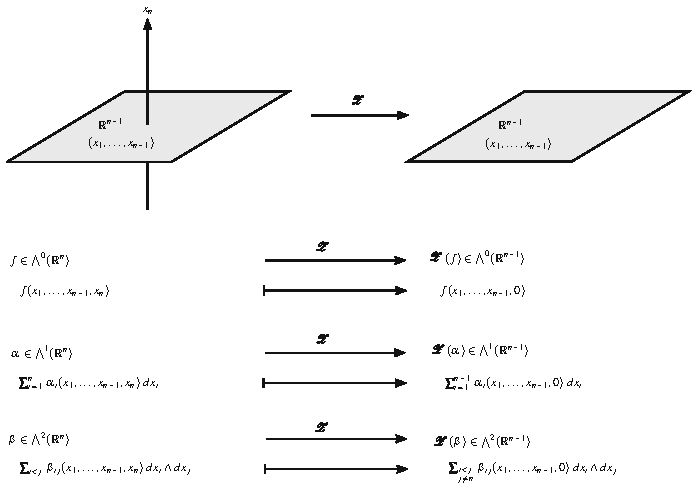
\includegraphics[width=0.960\linewidth]{images/vector/fig-8-7.pdf}
  \caption{映射 $Z:\Omega^k(\mathbb{R}^n)\to\Omega^k(\mathbb{R}^{n-1})$ 的图解. 该映射把 $\mathbb{R}^n$ 上的 $k$-形式``挤压''成 $\mathbb{R}^{n-1}$ 上的 $k$-形式. 这里对零形式、1-形式和 2-形式具体地展示了这一点. $Z$ 令 $x_n=0$ 并消去所有含有 $dx_n$ 的项}
  \label{fig:8-7}
\end{figure}

映射 $C$ 把 $\mathbb{R}^n$ 上的 $k$-形式``扩张''成 $\mathbb{R}^{n+1}$ 上的 $k$-形式，
\begin{align*}
f(x_1,\ldots,x_{n-1},x_n)\xrightarrow{\;C\;}f(x_1,\ldots,x_{n-1},x_n), \\
\sum_{i=1}^{n}\alpha_i(x_1,\ldots,x_{n-1},x_n)dx_i\xrightarrow{\;C\;}
\sum_{i=1}^{n}\alpha_i(x_1,\ldots,x_{n-1},x_n)dx_i, \\
\sum_{i<j}\beta_{ij}(x_1,\ldots,x_{n-1},x_n)dx_i\wedge dx_j\xrightarrow{\;C\;}
\sum_{i<j}\beta_{ij}(x_1,\ldots,x_{n-1},x_n)dx_i\wedge dx_j.
\end{align*}
见图 \ref{fig:8-8}.

\begin{figure}[htbp]
  \centering
  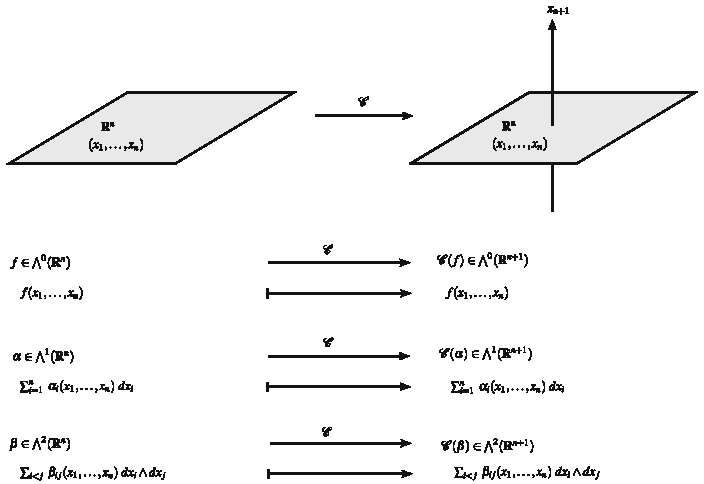
\includegraphics[width=0.960\linewidth]{images/vector/fig-8-8.pdf}
  \caption{映射 $C:\Omega^k(\mathbb{R}^n)\to\Omega^k(\mathbb{R}^{n+1})$ 的图解. 该映射把 $\mathbb{R}^n$ 上的 $k$-形式``扩张''成 $\mathbb{R}^{n+1}$ 上的 $k$-形式. 扩张后的 $\mathbb{R}^{n+1}$ 上的 $k$-形式看起来与 $\mathbb{R}^n$ 上的 $k$-形式完全一样. 这里对零形式、1-形式和 2-形式具体地展示了这一点}
  \label{fig:8-8}
\end{figure}

注意，$f\in\Omega^0(\mathbb{R}^n)$ 看起来与 $C(f)\in\Omega^0(\mathbb{R}^{n+1})$ 完全一样，后者就是一个不依赖于变量 $x_{n+1}$ 的函数. 类似地，$\alpha\in\Omega^1(\mathbb{R}^n)$ 看起来与 $C(\alpha)\in\Omega^1(\mathbb{R}^{n+1})$ 完全一样，后者是 $\mathbb{R}^{n+1}$ 上不含 $dx_{n+1}$ 项、且其分量函数 $\alpha_i$ 完全不依赖于变量 $x_{n+1}$ 的 1-形式. 对 2-形式 $\beta\in\Omega^2(\mathbb{R}^n)$ 也是如此. $C(\beta)$ 看起来与 $\beta$ 完全一样；它是 $\mathbb{R}^{n+1}$ 上不含任何涉及 $dx_{n+1}$ 的项、且其分量函数 $\beta_{ij}$ 不依赖于变量 $x_{n+1}$ 的 2-形式.

为了更好地看清楚这一点，考虑 1-形式 $\alpha=P(x,y,z)dx+Q(x,y,z)dy+R(x,y,z)dz\in\Omega^1(\mathbb{R}^3)$. 那么
\[
Z(\alpha)=P(x,y,0)dx+Q(x,y,0)dy\in\Omega^1(\mathbb{R}^2).
\]
注意我们消掉了含 $dz$ 的项，即 $R(x,y,z)dz$. 现在考虑 1-形式 $\alpha=P(x,y)dx+Q(x,y)dy\in\Omega^1(\mathbb{R}^2)$，那么
\[
C(\alpha)=P(x,y)dx+Q(x,y)dy\in\Omega^1(\mathbb{R}^3).
\]
这个 $\mathbb{R}^3$ 上的 1-形式看起来与 $\mathbb{R}^2$ 上的 1-形式完全一样，尽管它实际上是在 $\mathbb{R}^3$ 上. 它是 $\mathbb{R}^3$ 上不含 $dz$ 项、且分量函数不依赖于变量 $z$ 的 1-形式.

\begin{question}\label{q:8-1}
利用 $\alpha=P(x,y,z)dx+Q(x,y,z)dy+R(x,y,z)dz\in\Omega^1(\mathbb{R}^3)$，证明 $d(Z(\alpha))=Z(d(\alpha))$. 我们常把它写成 $dZ=Zd$.
\end{question}

\begin{question}\label{q:8-2}
利用 $\alpha=P(x,y)dx+Q(x,y)dy\in\Omega^1(\mathbb{R}^2)$，证明 $d(C(\alpha))=C(d(\alpha))$. 我们常把它写成 $dC=Cd$.
\end{question}

\begin{question}\label{q:8-3}
利用 $\alpha=P(x,y,z)dx+Q(x,y,z)dy+R(x,y,z)dz\in\Omega^1(\mathbb{R}^3)$，求 $Z(\alpha)$，然后求 $C(Z(\alpha))$.
\end{question}

除了 $Z$ 和 $C$，我们还需要定义另一个映射 $K:\Omega^1(\mathbb{R}^3)\to\Omega^0(\mathbb{R}^3)$. 若 $\alpha=P(x,y,z)dx+Q(x,y,z)dy+R(x,y,z)dz$ 是 $\mathbb{R}^3$ 上的 1-形式，则 $K(\alpha)$ 是一个零形式，即 $\mathbb{R}^3$ 上的函数，定义为
\[
K(\alpha)=K\left(P(x,y,z)dx+Q(x,y,z)dy+R(x,y,z)dz\right)=\int_0^z R(x,y,t)\,dt.
\]
换言之，$K(\alpha):\mathbb{R}^3\to\mathbb{R}$. 这实际上是如何运作的呢？若给定了 $\mathbb{R}^3$ 上的点 $p=(x_0,y_0,z_0)$，则
\[
K(\alpha)(p)=K(\alpha)(x_0,y_0,z_0)=\int_0^{z_0}R(x_0,y_0,t)\,dt\in\mathbb{R}.
\]

由于 Poincaré 引理讲的是证明闭形式是恰当的，在我们的证明中需要用到一些与闭形式相关的事实. 在这个中等难度的例子中，我们处理的是 $\mathbb{R}^3$ 上的闭 1-形式 $\alpha$. 我们将利用 $d\alpha=0$ 这一事实来找出证明过程中需要的一些恒等式.
\[
\begin{aligned}
d\alpha &= d\left(P(x,y,z)dx+Q(x,y,z)dy+R(x,y,z)dz\right)\\
&= dP\wedge dx+dQ\wedge dy+dR\wedge dz\\
&= \frac{\partial P}{\partial y}dy\wedge dx+\frac{\partial P}{\partial z}dz\wedge dx
  +\frac{\partial Q}{\partial x}dx\wedge dy+\frac{\partial Q}{\partial z}dz\wedge dy
  +\frac{\partial R}{\partial x}dx\wedge dz+\frac{\partial R}{\partial y}dy\wedge dz\\
&= \left(\frac{\partial Q}{\partial x}-\frac{\partial P}{\partial y}\right)dx\wedge dy
  +\left(\frac{\partial R}{\partial x}-\frac{\partial P}{\partial z}\right)dx\wedge dz
  +\left(\frac{\partial R}{\partial y}-\frac{\partial Q}{\partial z}\right)dy\wedge dz\\
&= 0
\end{aligned}
\]
因此这个 2-形式的每一项的系数都等于零，从而给出下面三个恒等式
\[
\frac{\partial Q}{\partial x}=\frac{\partial P}{\partial y},\qquad
\frac{\partial R}{\partial x}=\frac{\partial P}{\partial z},\qquad
\frac{\partial R}{\partial y}=\frac{\partial Q}{\partial z}.
\]

既然所有必要的准备终于落实了，我们就准备好在我们这个例子中证明 Poincaré 引理了. 我们首先给出总体策略. 之后我们给出每一步的细节. 假设我们知道 $\alpha\in\Omega^1(\mathbb{R}^3)$ 是闭的. 我们的目标是证明 $\alpha$ 也是恰当的. 也就是说，我们想证明存在某个 $\beta\in\Omega^0(\mathbb{R}^3)$ 使得 $d\beta=\alpha$. 首先我们给出我们想做什么的一般思路，图 \ref{fig:8-9} 给出了示意. 我们先用 $Z$ 把 $\alpha$``挤压''下来得到 $Z(\alpha)\in\Omega^1(\mathbb{R}^2)$，由归纳假设可以证明它是恰当的. 然后用 $C$ 把恰当形式 $Z(\alpha)$``扩张''得到 $C(Z(\alpha))\in\Omega^1(\mathbb{R}^3)$，它也可以被证明是恰当的. 由于 $C(Z(\alpha))$ 在某种意义上只是 $\alpha$ 的一部分，我们想证明 $\alpha$ 的其余部分，即 $\alpha-C(Z(\alpha))$，也是恰当的. 我们可以通过对 $\alpha$ 使用 $K$ 得到 $K(\alpha)\in\Omega^0(\mathbb{R}^3)$，然后取它的外微分得到 $d(K(\alpha))\in\Omega^1(\mathbb{R}^3)$，后者显然是恰当的. 事实证明
\[
\underbrace{d(K(\alpha))}_{\text{由定义显然恰当}}=\alpha-\underbrace{C(Z(\alpha))}_{\text{由归纳假设恰当}}.
\]
换言之，我们有
\[
d(K(\alpha))=\alpha-C(Z(\alpha)).
\]
但这就意味着
\[
\begin{aligned}
\alpha &= \underbrace{C(Z(\alpha))}_{\substack{\text{恰当，故存在某个 }\omega\\\text{使得 }C(Z(\alpha))=d\omega}}+\underbrace{d(K(\alpha))}_{\text{由定义显然恰当}}\\
&= d\omega+d(K(\alpha))\\
&= d\left(\omega+K(\alpha)\right)\qquad\text{（由 }d\text{ 的线性）}
\end{aligned}
\]
因此 $\alpha$ 本身是恰当的，这正是我们要证明的. 注意我们从未显式给出 $\omega$ 是什么. 换言之，虽然我们在逻辑上推理出 $\omega$ 必定存在，但我们从未真正找到 $\omega$ 的显式公式.

\begin{figure}[htbp]
  \centering
  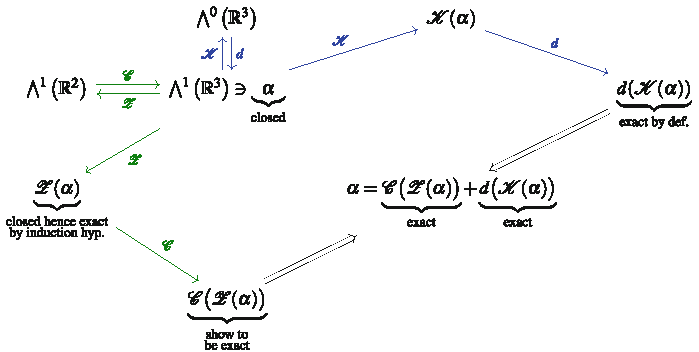
\includegraphics[width=0.960\linewidth]{images/vector/fig-8-9.pdf}
  \caption{我们例子证明的一般思路. 对 $\alpha\in\Omega^1(\mathbb{R}^3)$，我们计算 $K(\alpha)\in\Omega^0(\mathbb{R}^3)$，然后计算 $d(K(\alpha))\in\Omega^1(\mathbb{R}^3)$，后者显然是恰当的. 我们还计算 $Z(\alpha)\in\Omega^1(\mathbb{R}^2)$，它是闭的，因而由归纳假设是恰当的. 然后计算 $C(Z(\alpha))\in\Omega^1(\mathbb{R}^3)$，可以证明它也是恰当的. 于是可以证明 $\alpha=C(Z(\alpha))+d(K(\alpha))$，即两个恰当项之和，这意味着 $\alpha$ 本身是恰当的}
  \label{fig:8-9}
\end{figure}

现在我们已经把将要采用的总体策略告诉了你，就可以着手细节了. 我们现在需要证明两件事：第一，$C(Z(\alpha))$ 由归纳假设是恰当的；第二，$d(K(\alpha))=\alpha-C(Z(\alpha))$. 证明这两件事实际上正是整个证明的精华. 由于 $\alpha$ 是闭的，由闭的定义有 $d\alpha=0$. 利用 $dZ=Zd$ 这一事实，我们有
\[
d(Z(\alpha))=Z(d\alpha)=Z(0)=0\qquad\Rightarrow\qquad Z(\alpha)\in\Omega^1(\mathbb{R}^2)\ \text{是闭的}.
\]
归纳假设是说 $\mathbb{R}^2$ 上所有闭 1-形式都已知是恰当的. 由于 $Z(\alpha)$ 是 $\mathbb{R}^2$ 上已知是闭的 1-形式，由归纳假设我们知道 $Z(\alpha)$ 是恰当的. 这意味着 $\mathbb{R}^2$ 上存在某个零形式 $\omega$ 使得 $Z(\alpha)=d\omega$. 为了证明 $C(Z(\alpha))\in\Omega^1(\mathbb{R}^3)$ 是恰当的，我们利用 $dC=Cd$ 这一事实，
\[
C(Z(\alpha))=C(d\omega)=d(C\omega)\qquad\Rightarrow\qquad C(Z(\alpha))\in\Omega^1(\mathbb{R}^3)\ \text{是恰当的}.
\]
现在我们将证明 $d(K(\alpha))$ 是 $\alpha$ 减去恰当部分 $C(Z(\alpha))$ 后剩下的部分；也就是说，$d(K(\alpha))=\alpha-C(Z(\alpha))$. 这通过一个显式计算完成：
\[
\begin{aligned}
d(K(\alpha)) &= d\left(K\left(P(x,y,z)dx+Q(x,y,z)dy+R(x,y,z)dz\right)\right)\\
&= d\left(\int_0^z R(x,y,t)\,dt\right)\\
&= \frac{\partial}{\partial x}\left(\int_0^z R(x,y,t)\,dt\right)dx\\
&\qquad+\frac{\partial}{\partial y}\left(\int_0^z R(x,y,t)\,dt\right)dy\\
&\qquad+\frac{\partial}{\partial z}\left(\int_0^z R(x,y,t)\,dt\right)dz\\
&= \left(\int_0^z\frac{\partial R(x,y,t)}{\partial x}\,dt\right)dx\\
&\qquad+\left(\int_0^z\frac{\partial R(x,y,t)}{\partial y}\,dt\right)dy+R(x,y,z)\,dz\\
&\quad\text{（对 }x\text{、}y\text{ 的偏导可直接移入积分号内；最后一项由微积分基本定理）}\\
&= \left(\int_0^z\frac{\partial P(x,y,t)}{\partial t}\,dt\right)dx\\
&\qquad+\left(\int_0^z\frac{\partial Q(x,y,t)}{\partial t}\,dt\right)dy+R(x,y,z)\,dz\\
&\quad\text{（}\alpha\text{ 闭 }\Rightarrow\tfrac{\partial R}{\partial x}=\tfrac{\partial P}{\partial z}\text{，}\alpha\text{ 闭 }\Rightarrow\tfrac{\partial R}{\partial y}=\tfrac{\partial Q}{\partial z}\text{）}\\
&= \left(P(x,y,z)-P(x,y,0)\right)dx+\left(Q(x,y,z)-Q(x,y,0)\right)dy+R(x,y,z)\,dz\\
&= \left(P(x,y,z)dx+Q(x,y,z)dy+R(x,y,z)dz\right)-\left(P(x,y,0)dx+Q(x,y,0)dy\right)\\
&= \alpha-C(Z(\alpha))
\end{aligned}
\]
于是
\begin{align*}
d(K(\alpha))=\alpha-C(Z(\alpha)) \\
\Rightarrow\quad \alpha=d(K(\alpha))+C(Z(\alpha)),
\end{align*}
其中 $\underbrace{d(K(\alpha))\ \text{由定义恰当}}_{}$，$\underbrace{C(Z(\alpha))\ \text{由上面恰当}}_{}$.
\[
\Rightarrow\qquad \alpha\ \text{是恰当的}.
\]
这样我们就在我们的例子中证明了 Poincaré 引理. 我们证明了若 $\alpha\in\Omega^1(\mathbb{R}^3)$ 是闭的，则 $\alpha$ 也是恰当的.

现在有几条评注. 在 Poincaré 引理的一般证明中，我们将证明若 $\alpha$ 是 $\mathbb{R}^n$ 上的闭 $k$-形式，则它是恰当的. 我们的证明要求我们假设所谓的归纳假设. 在这里，为了证明 $\mathbb{R}^n$ 上的闭 $k$-形式是恰当的，我们利用 $\mathbb{R}^{n-1}$ 上的闭 $k$-形式是恰当的这一事实. 由我们的基础情形，我们已经证明了 $\mathbb{R}^0$ 上任何闭 $k$-形式都是恰当的.

一般证明对任意 $n$ 成立，所以若取 $n=1$，我们就能证明 $\mathbb{R}^1$ 上任何闭 $k$-形式都是恰当的. 我们在 Poincaré 引理的一般证明中证明这一点，这要求我们使用归纳假设. 在 $n=1$ 的情形中，我们的归纳假设是 $\mathbb{R}^0$ 上任何闭 $k$-形式都是恰当的，这我们已经知道了. 然后，一旦我们知道这一点，就可以用它来证明 $\mathbb{R}^1$ 上闭 $k$-形式是恰当的. 一旦这已知，同样的论证可以用来证明 $\mathbb{R}^2$ 上闭 $k$-形式是恰当的，这又可以用来证明 $\mathbb{R}^3$ 上闭 $k$-形式是恰当的，这又可以用来……如此等等. 这样我们就可以自举而上，证明我们想要的任何 $\mathbb{R}^n$ 上闭 $k$-形式都是恰当的.

当然，我们不想把同样的论证一遍又一遍地重复无穷多次，所以我们只做一次，但做的方式要足够一般，使之对我们想要的任何 $k$ 和 $n$ 的值都成立. 这意味着我们的记号必须非常一般，这可能会让我们的论证在记号上有点压得人喘不过气. 这就是我们为什么先做一个简单例子的原因之一，这样你可以在不被试图跟上所有记号分心的情况下感受论证的运作方式. 我们还要说明，如果我们对例子中所做的稍作改动，一般证明会更容易. 等时机成熟时我们会解释这一点.

\section{一般情形}

在 Poincaré 引理证明的一般情形中，我们将证明对任意的 $k$ 和 $n$，$\mathbb{R}^{n+1}$ 上的闭 $k$-形式都是恰当的. 但在投入一般情形的证明之前，让我们重新审视一下 $Z$ 和 $C$ 这两个映射，确保我们理解它们是什么，以及它们对任意 $k$ 和 $n$ 如何运作. 事实证明，$Z$ 和 $C$ 是两个简单映射的\newterm{pull-back}{拉回}{pull-back}. 我们先考察 $Z$.

考虑图 \ref{fig:8-10} 所示的记为 $S$ 的拉伸映射，
\[
S:\mathbb{R}^n\to\mathbb{R}^{n+1},\qquad (x_1,\ldots,x_n)\longmapsto(x_1,\ldots,x_n,0).
\]
注意这里有些歧义. 除了把 $x_i$ 既用作坐标函数的记号又用作数值之外，我们还把 $x_i$ 用作 $\mathbb{R}^n$ 和 $\mathbb{R}^{n+1}$ 两个空间的坐标函数. 我们想稍微小心一点，在头脑中把空间区分开来，所以我们说 $x_1,\ldots,x_n$ 是 $\mathbb{R}^n$ 上的坐标函数，$y_1,\ldots,y_{n+1}$ 是 $\mathbb{R}^{n+1}$ 上的坐标函数. 严格地说我们会写
\[
S:\mathbb{R}^n\to\mathbb{R}^{n+1},\qquad
(x_1,\ldots,x_n)\longmapsto\left(y_1(x_1,\ldots,x_n),\ldots,y_{n+1}(x_1,\ldots,x_n)\right),
\]
其中
\[
y_1(x_1,\ldots,x_n)=x_1,\quad\ldots\quad
y_n(x_1,\ldots,x_n)=x_n,\quad
y_{n+1}(x_1,\ldots,x_n)=0.
\]
当然，映射 $S$ 给出 $k$-形式的拉回映射 $T^*S\equiv S^*$，
\[
\Omega^k(\mathbb{R}^{n+1})\xleftarrow{\;T^*S\;}\Omega^k(\mathbb{R}^n),\qquad
S:\mathbb{R}^n\to\mathbb{R}^{n+1}.
\]
这显示在图 \ref{fig:8-11} 中.

\begin{figure}[htbp]
  \centering
  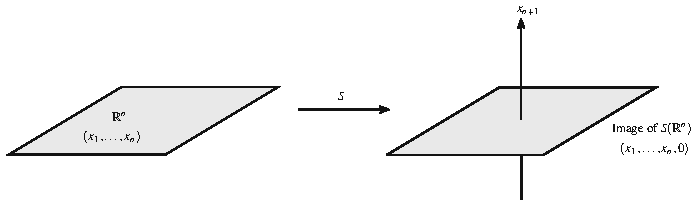
\includegraphics[width=0.960\linewidth]{images/vector/fig-8-10.pdf}
  \caption{映射 $S:\mathbb{R}^n\to\mathbb{R}^{n+1}$}
  \label{fig:8-10}
\end{figure}

$\mathbb{R}^{n+1}$ 上 $k$-形式的基本构件具有形式 $f_{i_1\cdots i_k}dy_{i_1}\wedge dy_{i_2}\wedge\cdots\wedge dy_{i_k}$，其中按约定有 $i_1<i_2<\cdots<i_k\leq n+1$. 利用第 6.7 节中第二和第三个恒等式，并利用零形式的拉回（也在第 6.7 节讲过），我们计算这些 $k$-形式基本构件之一的拉回，
\[
\begin{aligned}
&T^*S\cdot\left(f_{i_1\cdots i_k}dy_{i_1}\wedge dy_{i_2}\wedge\cdots\wedge dy_{i_k}\right)\\
&= T^*Sf_{i_1\cdots i_k}\cdot T^*Sdy_{i_1}\wedge T^*Sdy_{i_2}\wedge\cdots\wedge T^*Sdy_{i_k}\\
&= (f_{i_1\cdots i_k}\circ S)\cdot d(S^*y_{i_1})\wedge d(S^*y_{i_2})\wedge\cdots\wedge d(S^*y_{i_k})\\
&= (f_{i_1\cdots i_k}\circ S)\cdot d(y_{i_1}\circ S)\wedge d(y_{i_2}\circ S)\wedge\cdots\wedge d(y_{i_k}\circ S)\\
&= (f_{i_1\cdots i_k}\circ S)\cdot\left(\sum_{j=1}^{n}\frac{\partial y_{i_1}(x_1,\ldots,x_n)}{\partial x_j}dx_j\right)
  \wedge\cdots\wedge\left(\sum_{j=1}^{n}\frac{\partial y_{i_k}(x_1,\ldots,x_n)}{\partial x_j}dx_j\right)\\
&=\begin{cases}
f_{i_1\cdots i_k}(x_1,\ldots,x_n,0)\,dx_{i_1}\wedge\cdots\wedge dx_{i_k}, & \text{若 } i_k\neq n+1,\\
0, & \text{若某个 } i=n+1.
\end{cases}
\end{aligned}
\]
最后一个等式由 $y_i(x_1,\ldots,x_n)$ 的定义得出. 对每个满足 $1\leq i_l\leq n+1$ 的 $i_l$，我们有
\[
\sum_{j=1}^{n}\frac{\partial y_i(x_1,\ldots,x_n)}{\partial x_j}dx_j=
\begin{cases}
\displaystyle\sum_{j=1}^{n}\frac{\partial x_i}{\partial x_j}dx_j=dx_i, & \text{若 } i\neq n+1,\\
\displaystyle\sum_{j=1}^{n}\frac{\partial 0}{\partial x_j}dx_j=0, & \text{若 } i=n+1.
\end{cases}
\]
这正是我们之前的映射 $Z$，因此 $Z=T^*S$. 用这个公式以及拉回的线性（即第 6.7 节的第一个恒等式），可以拉回完整的 $k$-形式. 换言之，只需把这个公式应用于 $k$-形式的每一项即可.

\begin{figure}[htbp]
  \centering
  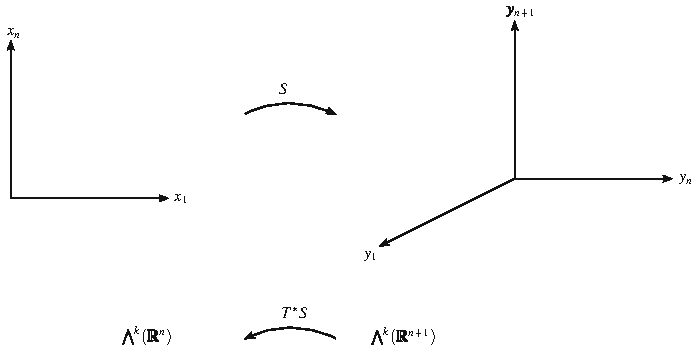
\includegraphics[width=0.960\linewidth]{images/vector/fig-8-11.pdf}
  \caption{用更合适的坐标函数记号表示的映射 $S:\mathbb{R}^n\to\mathbb{R}^{n+1}$，以及拉回映射 $T^*S\equiv S^*:\Omega^k(\mathbb{R}^{n+1})\to\Omega^k(\mathbb{R}^n)$}
  \label{fig:8-11}
\end{figure}

\begin{question}\label{q:8-4}
对 $S:\mathbb{R}^2\to\mathbb{R}^3$ 和 $\alpha=P(x,y,z)dx+Q(x,y,z)dy+R(x,y,z)dz\in\Omega^1(\mathbb{R}^3)$，证明上面定义的 $T^*S\cdot\alpha$ 与 $Z(\alpha)$ 相同.
\end{question}

现在我们转向 $C$. 现在我们考虑另一个不同的映射——投影映射，记为 $P$，如图 \ref{fig:8-12} 所示，
\[
P:\mathbb{R}^{n+1}\to\mathbb{R}^n,\qquad
(y_1,\ldots,y_{n+1})\longmapsto\left(x_1(y_1,\ldots,y_{n+1}),\ldots,x_n(y_1,\ldots,y_{n+1})\right),
\]
其中
\[
x_1(y_1,\ldots,y_{n+1})=y_1,\quad\ldots\quad
x_n(y_1,\ldots,y_{n+1})=y_n.
\]
这就给出拉回映射 $T^*P\equiv P^*$，
\[
\Omega^k(\mathbb{R}^{n+1})\xleftarrow{\;T^*P\;}\Omega^k(\mathbb{R}^n),\qquad
P:\mathbb{R}^{n+1}\to\mathbb{R}^n.
\]
$\mathbb{R}^n$ 上 $k$-形式的基本构件是 $f_{i_1\cdots i_k}dx_{i_1}\wedge\cdots\wedge dx_{i_k}$，其中 $i_1<i_2<\cdots<i_k$. 我们计算
\[
\begin{aligned}
&T^*P\cdot\left(f_{i_1\cdots i_k}dx_{i_1}\wedge\cdots\wedge dx_{i_k}\right)\\
&= (T^*Pf_{i_1\cdots i_k})\cdot T^*Pdx_{i_1}\wedge\cdots\wedge T^*Pdx_{i_k}\\
&= (f_{i_1\cdots i_k}\circ P)\cdot d(T^*Px_{i_1})\wedge\cdots\wedge d(T^*Px_{i_k})\\
&= (f_{i_1\cdots i_k}\circ P)\cdot d(x_{i_1}\circ P)\wedge\cdots\wedge d(x_{i_k}\circ P)\\
&= f_{i_1\cdots i_k}(y_1,\ldots,y_{n+1})\,dy_{i_1}\wedge\cdots\wedge dy_{i_k}.
\end{aligned}
\]
因此我们看到我们的映射恰好就是 $C=P^*$.

\begin{figure}[htbp]
  \centering
  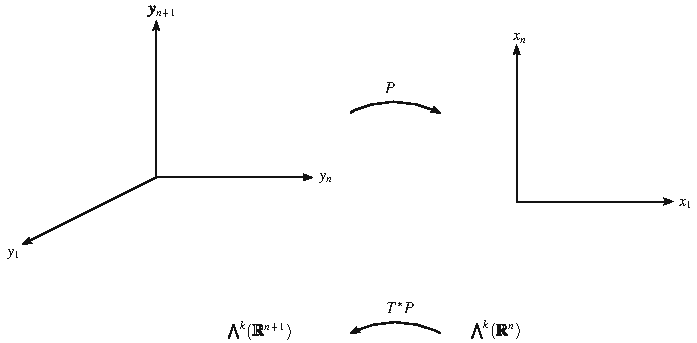
\includegraphics[width=0.960\linewidth]{images/vector/fig-8-12.pdf}
  \caption{映射 $P:\mathbb{R}^{n+1}\to\mathbb{R}^n$ 以及拉回映射 $T^*P\equiv P^*:\Omega^k(\mathbb{R}^n)\to\Omega^k(\mathbb{R}^{n+1})$}
  \label{fig:8-12}
\end{figure}

\begin{question}\label{q:8-5}
证明上面的最后一个等式，也就是说，对 $1\leq l\leq k\leq n$ 证明 $dx_{i_l}=dy_{i_l}$.
\end{question}

\begin{question}\label{q:8-6}
证明对任意 $k$-形式 $\beta$ 有 $Z(C(\beta))=\beta$.
\end{question}

由于 $C=P^*$、$Z=S^*$，并且我们已经从拉回和外微分的性质知道 $dP^*=P^*d$、$dS^*=S^*d$，所以我们自动得到 $dC=Cd$ 和 $dZ=Zd$.

在一般情形中，映射 $K:\Omega^k(\mathbb{R}^{n+1})\to\Omega^{k-1}(\mathbb{R}^{n+1})$ 由下式给出
若 $i_k\neq n+1$，则
\[
K\left(f(x_1,\ldots,x_{n+1})dx_{i_1}\wedge\cdots\wedge dx_{i_k}\right)=0.
\]
若 $i_k=n+1$，则
\[
K\left(f(x_1,\ldots,x_{n+1})dx_{i_1}\wedge\cdots\wedge dx_{i_k}\right)
=\left(\int_0^{x_{n+1}}f(x_1,\ldots,x_n,t)\,dt\right)dx_{i_1}\wedge\cdots\wedge dx_{i_{k-1}}.
\]
映射 $K:\Omega^{k+1}(\mathbb{R}^{n+1})\to\Omega^k(\mathbb{R}^{n+1})$ 是类似的，只是做了相应调整.

我们现在准备证明 Poincaré 引理的一般情形. 假设我们有 $\alpha\in\Omega^k(\mathbb{R}^{n+1})$，它是闭的. 也就是说，$d\alpha=0$. 我们将用到的各种映射显示在图 \ref{fig:8-13} 的上方，我们要做什么的一般示意显示在下方. 在例子中我们证明了 $\alpha=CZ\alpha+d(K\alpha)$. 我们还证明了 $CZ\alpha$ 是恰当的，并且显然 $d(K\alpha)$ 是恰当的，所以可以推出 $\alpha$ 是恰当的. 事实证明，在一般情形中，证明更一般的结论反而更容易：对任意闭 $k$-形式 $\alpha$ 都有
\[
\alpha=CZ\alpha+(-1)^{k-1}\left(d(K\alpha)+Kd\alpha\right)
=\left(CZ+(-1)^{k-1}(dK+Kd)\right)\alpha.
\]
我们为什么要这样做呢？问题在于，一般来说 $\mathbb{R}^{n+1}$ 上的 $k$-形式 $\alpha$ 具有形式
\[
\alpha=\sum\alpha_{j_1\cdots j_k}(x_1,x_2,\ldots,x_{n+1})dx_{j_1}\wedge\cdots\wedge dx_{j_k},
\]
其中每个 $\alpha_{j_1\cdots j_k}$ 都是实值函数，当然还有 $j_1<\cdots<j_k$. 虽然 $\alpha$ 整体可能是闭的，但和式中的每一项未必是闭的，事实上很可能不是闭的. 这正是问题所在. 为简单起见，我们希望证明中的计算一次只对和式中的一项进行. 也就是说，我们希望分别对和式中的每一项 $\alpha_{j_1\cdots j_k}(x_1,x_2,\ldots,x_{n+1})dx_{j_1}\wedge\cdots\wedge dx_{j_k}$ 进行计算. 能够这样做会使计算简单得多. 然后我们可以只用线性把我们的结果应用于整个 $\alpha$，它只是各项之和.

\begin{figure}[htbp]
  \centering
  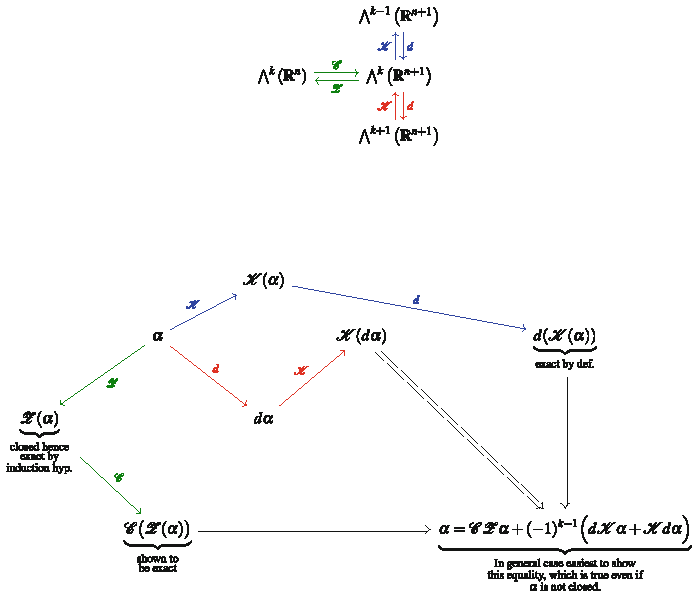
\includegraphics[width=0.960\linewidth]{images/vector/fig-8-13.pdf}
  \caption{Poincaré 引理一般情形证明中重要的各种映射显示在上方，一般情形证明的示意图显示在下方. 回顾 $k$-形式 $\alpha$ 具有形式 $\alpha=\sum\alpha_{i_1\cdots i_k}dx_{i_1}\wedge\cdots\wedge dx_{i_k}$，其中每个 $\alpha_{i_1\cdots i_k}$ 是流形上的函数. 虽然整个 $k$-形式 $\alpha$ 可能是闭的，但组成 $\alpha$ 的每一项 $\alpha_{i_1\cdots i_k}dx_{i_1}\wedge\cdots\wedge dx_{i_k}$ 却未必是闭的. 推导出的公式 $\alpha=CZ\alpha+(-1)^{k-1}(dK\alpha+Kd\alpha)$ 对其中每一项成立. 利用线性，该公式对 $\alpha$ 整体成立；若 $\alpha$ 是闭的，则公式化为 $\alpha=CZ\alpha+(-1)^{k-1}dK\alpha$，后者被证明是恰当的}
  \label{fig:8-13}
\end{figure}

证明的第一部分——证明 $CZ\alpha$ 是恰当的——与之前相同. 由于 $\alpha$ 是闭的，由闭的定义有 $d\alpha=0$，于是
\[
d(C\alpha)=C(d\alpha)=C(0)=0,
\]
所以 $C\alpha$ 也是闭的. 但 $C\alpha\in\Omega^k(\mathbb{R}^n)$，而我们的归纳假设是 $\mathbb{R}^n$ 上所有闭形式都是恰当的. 由归纳假设，由于 $C\alpha$ 是闭的，它也是恰当的，所以对某个 $\beta$ 有 $C\alpha=d\beta$. 于是
\[
ZC\alpha=Zd\beta=dZ\beta.
\]
但这意味着 $ZC\alpha$ 是形式 $Z\beta$ 的外微分，由恰当性的定义，这意味着 $ZC\alpha$ 是恰当的. 这样我们就证明了若 $\alpha$ 是闭的，则 $ZC\alpha$ 是恰当的.

现在我们转向要证明的恒等式. 我们需要把对 $\alpha$ 的一个基本构件元素的证明分成两种情形，一种 $j_k=n+1$，一种 $j_k\neq n+1$.

\textbf{情形一：} $j_k=n+1$

我们考虑单项形式 $f(x_1,\ldots,x_{n+1})dx_{j_1}\wedge\cdots\wedge dx_{j_k}$，其中 $j_1<j_2<\cdots<j_k$ 且 $j_k=n+1$，
\[
\begin{aligned}
&dK\left(f(x_1,\ldots,x_{n+1})dx_{j_1}\wedge\cdots\wedge dx_{j_k}\right)\\
&= d\left(\int_0^{x_{n+1}}f(x_1,\ldots,x_n,t)\,dt\,dx_{j_1}\wedge\cdots\wedge dx_{j_{k-1}}\right)\\
&= \sum_{i=1}^{n+1}\frac{\partial}{\partial x_i}\left(\int_0^{x_{n+1}}f(x_1,\ldots,x_n,t)\,dt\right)dx_i\wedge dx_{j_1}\wedge\cdots\wedge dx_{j_{k-1}}\\
&= \sum_{i=1}^{n}\left(\int_0^{x_{n+1}}\frac{\partial f(x_1,\ldots,x_n,t)}{\partial x_i}\,dt\right)dx_i\wedge dx_{j_1}\wedge\cdots\wedge dx_{j_{k-1}}\\
&\qquad +f(x_1,\ldots,x_{n+1})\,dx_{n+1}\wedge dx_{j_1}\wedge\cdots\wedge dx_{j_{k-1}}.
\end{aligned}
\]
接下来计算
\[
\begin{aligned}
&Kd\left(f(x_1,\ldots,x_{n+1})dx_{j_1}\wedge\cdots\wedge dx_{j_k}\right)\\
&= K\left(\sum_{i=1}^{n+1}\frac{\partial f(x_1,\ldots,x_{n+1})}{\partial x_i}dx_i\wedge dx_{j_1}\wedge\cdots\wedge dx_{j_k}\right)\\
&= \sum_{i=1}^{n}K\left(\frac{\partial f(x_1,\ldots,x_{n+1})}{\partial x_i}dx_i\wedge dx_{j_1}\wedge\cdots\wedge dx_{j_k}\right)\\
&= \sum_{i=1}^{n}\left(\int_0^{x_{n+1}}\frac{\partial f(x_1,\ldots,x_n,t)}{\partial x_i}\,dt\right)dx_i\wedge dx_{j_1}\wedge\cdots\wedge dx_{j_k}.
\end{aligned}
\]
将第一个式子减去第二个式子，并回忆 $j_k=n+1$，再注意到
\[
CZ\left(f(x_1,\ldots,x_{n+1})dx_{j_1}\wedge\cdots\wedge dx_{j_{k-1}}\wedge dx_{n+1}\right)=0,
\]
我们得到
\[
\begin{aligned}
&(dK-Kd)\left(f(x_1,\ldots,x_{n+1})dx_{j_1}\wedge\cdots\wedge dx_{j_k}\right)\\
&= f(x_1,\ldots,x_{n+1})dx_{n+1}\wedge dx_{j_1}\wedge\cdots\wedge dx_{j_{k-1}}\\
&= (-1)^{k-1}f(x_1,\ldots,x_{n+1})dx_{j_1}\wedge\cdots\wedge dx_{j_{k-1}}\wedge dx_{n+1}-0\\
&= (-1)^{k-1}\left(1-CZ\right)\left(f(x_1,\ldots,x_{n+1})dx_{j_1}\wedge\cdots\wedge dx_{j_{k-1}}\wedge dx_{n+1}\right).
\end{aligned}
\]
稍作整理，并记 $\omega=f(x_1,\ldots,x_{n+1})dx_{j_1}\wedge\cdots\wedge dx_{j_k}$（它本身实际上未必是闭的），就得到我们想要的，即
\[
\omega=CZ\omega+(-1)^{k-1}\left(dK\omega-Kd\omega\right).
\]

\begin{question}\label{q:8-7}
证明 $CZ\left(f(x_1,\ldots,x_{n+1})dx_{j_1}\wedge\cdots\wedge dx_{j_{k-1}}\wedge dx_{n+1}\right)=0$.
\end{question}

\textbf{情形二：} $j_k\neq n+1$

我们考虑单项形式 $f(x_1,\ldots,x_{n+1})dx_{j_1}\wedge\cdots\wedge dx_{j_k}$，其中 $j_1<j_2<\cdots<j_k$ 但 $j_k\neq n+1$. 这里，由映射 $K$ 的定义，我们有
\[
dK\left(f(x_1,\ldots,x_{n+1})dx_{j_1}\wedge\cdots\wedge dx_{j_k}\right)=0.
\]
现在我们计算
\[
\begin{aligned}
&Kd\left(f(x_1,\ldots,x_{n+1})dx_{j_1}\wedge\cdots\wedge dx_{j_k}\right)\\
&= K\left(\sum_{i=1}^{n+1}\frac{\partial f(x_1,\ldots,x_{n+1})}{\partial x_i}dx_i\wedge dx_{j_1}\wedge\cdots\wedge dx_{j_k}\right)\\
&= K\Biggl(\sum_{i=1}^{n}\frac{\partial f(x_1,\ldots,x_{n+1})}{\partial x_i}dx_i\wedge dx_{j_1}\wedge\cdots\wedge dx_{j_k}\\
&\quad+\frac{\partial f(x_1,\ldots,x_{n+1})}{\partial x_{n+1}}dx_{n+1}\wedge dx_{j_1}\wedge\cdots\wedge dx_{j_k}\Biggr)\\
&\quad\text{（}K\text{ 消去所有这些不含 }dx_{n+1}\text{ 的项）}\\
&= K\left((-1)^k\frac{\partial f(x_1,\ldots,x_{n+1})}{\partial x_{n+1}}dx_{j_1}\wedge\cdots\wedge dx_{j_k}\wedge dx_{n+1}\right)\\
&= (-1)^k\left(\int_0^{x_{n+1}}\frac{\partial f(x_1,\ldots,x_n,t)}{\partial x_{n+1}}\,dt\right)dx_{j_1}\wedge\cdots\wedge dx_{j_k}\\
&= (-1)^k\left(f(x_1,\ldots,x_n,x_{n+1})-f(x_1,\ldots,x_n,0)\right)dx_{j_1}\wedge\cdots\wedge dx_{j_k}\\
&\quad\text{（微积分基本定理）}
\end{aligned}
\]
将第二个式子从第一个式子中减去，得到
\[
\begin{aligned}
&(dK-Kd)\left(f(x_1,\ldots,x_{n+1})dx_{j_1}\wedge\cdots\wedge dx_{j_k}\right)\\
&= 0-(-1)^k\left(f(x_1,\ldots,x_n,x_{n+1})-f(x_1,\ldots,x_n,0)\right)dx_{j_1}\wedge\cdots\wedge dx_{j_k}\\
&= (-1)^{k-1}\left(f(x_1,\ldots,x_n,x_{n+1})dx_{j_1}\wedge\cdots\wedge dx_{j_k}-f(x_1,\ldots,x_n,0)dx_{j_1}\wedge\cdots\wedge dx_{j_k}\right).
\end{aligned}
\]
但若 $j_k\neq n+1$，则
\[
CZ\left(f(x_1,\ldots,x_{n+1})dx_{j_1}\wedge\cdots\wedge dx_{j_k}\right)=f(x_1,\ldots,x_n,0)dx_{j_1}\wedge\cdots\wedge dx_{j_k},
\]
所以令 $\omega=f(x_1,\ldots,x_{n+1})dx_{j_1}\wedge\cdots\wedge dx_{j_k}$，我们有
\begin{align*}
(dK-Kd)\omega=(-1)^{k-1}\left(\omega-CZ\omega\right) \\
\Rightarrow\qquad \omega=CZ\omega+(-1)^{k-1}\left(dK\omega-Kd\omega\right),
\end{align*}
这与情形一中得到的公式完全相同.

因此，无论 $j_k=n+1$ 还是 $j_k\neq n+1$，对 $k$-形式 $\alpha$ 的每一项 $\omega$ 我们都得到完全相同的恒等式，即
\[
\omega=CZ\omega+(-1)^{k-1}\left(dK\omega-Kd\omega\right).
\]
因此这个公式对 $k$-形式 $\alpha$ 中的每一项都成立. 现在我们可以完成 Poincaré 引理的证明了. 我们把证明中的几个步骤留给你在下面的问题中完成.

\begin{question}\label{q:8-8}
证明映射 $Z$、$C$ 和 $K$ 是线性的. 也就是说，证明若 $\alpha$ 和 $\beta$ 是 $k$-形式，则 $Z(\alpha+\beta)=Z(\alpha)+Z(\beta)$、$C(\alpha+\beta)=C(\alpha)+C(\beta)$、$K(\alpha+\beta)=K(\alpha)+K(\beta)$.
\end{question}

\begin{question}\label{q:8-9}
利用 $C$、$Z$、$K$ 和 $d$ 的线性，证明恒等式
\[
\omega=CZ\omega+(-1)^{k-1}\left(dK\omega-Kd\omega\right)
\]
适用于一般的 $k$-形式
\[
\alpha=\sum\alpha_{j_1\cdots j_k}dx_{j_1}\wedge\cdots\wedge dx_{j_k}.
\]
\end{question}

由上面的问题，对一般的 $k$-形式 $\alpha$ 有 $\alpha=CZ\alpha+(-1)^{k-1}\left(dK\alpha-Kd\alpha\right)$. 为证明 $\mathbb{R}^{n+1}$ 上的闭 $k$-形式是恰当的，我们由归纳假设假设 $\mathbb{R}^n$ 上的闭 $k$-形式是恰当的. 归纳假设被用来证明：若 $\alpha$ 是闭的，则 $CZ\alpha$ 是恰当的，所以存在 $\beta$ 使得 $CZ\alpha=d\beta$. 另外，由于 $\alpha$ 是闭的，有 $Kd\alpha=0$，所以
\[
\begin{aligned}
\alpha &= CZ\alpha+(-1)^{k-1}\left(dK\alpha-\underbrace{Kd\alpha}_{=0}\right)\\
&= d\beta+(-1)^{k-1}\left(dK\alpha-0\right)\\
&= d\beta+d\left((-1)^{k-1}K\alpha\right)\\
&= d\left(\beta+(-1)^{k-1}K\alpha\right)
\end{aligned}
\]
所以 $\alpha$ 是恰当的.

\begin{question}\label{q:8-10}
利用图 \ref{fig:8-5} 和图 \ref{fig:8-13} 中的图更详细地解释，归纳假设以及推导出的公式如何使我们能够得出结论：任何 $\mathbb{R}^n$ 上的每个闭 $k$-形式都是恰当的.
\end{question}

\section{小结、参考文献与问题}

\subsection{小结}

Poincaré 引理断言 $\mathbb{R}^n$ 上的每个闭形式都是恰当的. 若 $d\alpha=0$，则微分形式 $\alpha$ 称为闭的. 若存在另一个微分形式 $\beta$ 使得 $\alpha=d\beta$，则微分形式 $\alpha$ 称为恰当的. 显然，若 $\alpha$ 是恰当的 $k$-形式，则 $\beta$ 必是 $(k-1)$-形式. 因此，Poincaré 引理还可以表述为：若 $\alpha$ 是 $\mathbb{R}^n$ 上满足 $d\alpha=0$ 的 $k$-形式，则存在某个 $(k-1)$-形式 $\beta$ 使得 $\alpha=d\beta$.

\subsection{参考文献与进一步阅读}

Poincaré 引理对任何讨论流形上微积分的书来说都是绝对必需的材料. 特别地，Munkres~\cite{ref35}、Renteln~\cite{ref37} 以及 Abraham、Marsden 和 Ratiu~\cite{ref01} 的著作都是很好的讲述. 数学中常有这样的情况：有了正确的数学概念、工具和技巧，许多定理的证明可以压缩成寥寥几行. Poincaré 引理正是如此. 本书这里的讲述虽然很长，但意在让数学背景只比微积分稍多一点的人也能容易理解. 而大多数其他 Poincaré 引理的讲述通常并非如此.

\subsection{问题}

\begin{question}\label{q:8-11}
证明下面每一个 1-形式 $\alpha_i$ 都是闭的；也就是说，证明 $d\alpha_i=0$. 由 Poincaré 引理，$\alpha_i$ 必是恰当的. 然后求函数 $f_i$ 使得 $\alpha_i=df_i$.
\begin{enumerate}
  \item[(a)] $\alpha_1=y^2dx+2xy\,dy$
  \item[(b)] $\alpha_2=(3x^2+y)dx+(x+2y)dy$
  \item[(c)] $\alpha_3=2x\,dx+3y^2dy+4z^3dz$
  \item[(d)] $\alpha_4=2xy\,dx+(x^2+2y+z)dy+(y-3z^2)dz$
  \item[(e)] $\alpha_5=(6x^2z-yz)dx+(3z^4-xz)dy+(2x^3+12yz^3-xy)dz$
  \item[(f)] $\alpha_6=(3y^2-4z^4)dx+6xy\,dy-16xz^3dz$
\end{enumerate}
\end{question}

\begin{question}\label{q:8-12}
证明下面每一个 2-形式 $\beta_i$ 都是闭的；也就是说，证明 $d\beta_i=0$. 由 Poincaré 引理，$\beta_i$ 必是恰当的. 求 1-形式 $\alpha_i$ 使得 $\beta_i=d\alpha_i$.
\begin{enumerate}
  \item[(a)] $\beta_1=24x^3y^2dx\wedge dy$
  \item[(b)] $\beta_2=(6x^2y-3xy^2)dx\wedge dy$
  \item[(c)] $\beta_3=8x^3y^3dy\wedge dz-6x^2y^4dz\wedge dx$
  \item[(d)] $\beta_4=(2x-1)dx\wedge dy+(3y^2-2z)dy\wedge dz+(1-3x^2)dz\wedge dx$
  \item[(e)] $\beta_5=-4xy^2dx\wedge dy+2x^2y^2dy\wedge dz+3xz^2dz\wedge dx$
  \item[(f)] $\beta_6=-4xy\,dx\wedge dy+2yz\,dy\wedge dz-2xz\,dz\wedge dx$
\end{enumerate}
\end{question}

\begin{question}\label{q:8-13}
证明下面每一个 3-形式 $\gamma_i$ 都是闭的；也就是说，证明 $d\gamma_i=0$. 由 Poincaré 引理，$\gamma_i$ 必是恰当的. 求 2-形式 $\beta_i$ 使得 $\gamma_i=d\beta_i$.
\begin{enumerate}
  \item[(a)] $\gamma_1=12x^2y^3z^4dx\wedge dy\wedge dz$
  \item[(b)] $\gamma_2=(x^3-4y+z^2)dx\wedge dy\wedge dz$
  \item[(c)] $\gamma_3=(2xz+3yz^2)dx\wedge dy\wedge dz$
  \item[(d)] $\gamma_4=2(x+y+z)dx\wedge dy\wedge dz$
\end{enumerate}
\end{question}

% 第 9 章 向量分析与微分形式
\chapter{向量分析与微分形式}

在第 1 至第 3 节中，我们从几何的观点仔细考察向量微积分中的\newterm{divergence}{散度}{divergence}、\newterm{curl}{旋度}{curl}和\newterm{gradient}{梯度}{gradient}，引入并定义三者. 在第 4 节中，我们引入一些记号并考虑两个重要的算子——升号算子和降号算子. 理解散度、旋度、梯度与微分形式之间的关系需要这些算子，这种关系将在第 5 节中考察. 同样在第 5 节中，我们将看到线积分基本定理、散度定理和向量微积分版本的 Stokes 定理如何都能用微分形式记号写成相同的形式. 这三个定理都是所谓的广义 Stokes 定理的特殊情形. 在更高级的数学课程中，Stokes 定理总是指广义 Stokes 定理，而不是你在向量微积分中学到的那个版本的 Stokes 定理，而在物理学中，Stokes 定理可能指两者中的任何一个，取决于上下文. 但请记住，从更抽象的观点来看，它们实际上是同一个定理.

\section{散度}

在向量微积分中，$\mathbb{R}^3$ 上的向量场 $F$ 通常写成 $F=P(x,y,z)\hat{\imath}+Q(x,y,z)\hat{\jmath}+R(x,y,z)\hat{k}$，其中 $P,Q,R:\mathbb{R}^3\to\mathbb{R}$. 这里 $\hat{\imath}$、$\hat{\jmath}$ 和 $\hat{k}$ 分别是 $x$、$y$、$z$ 方向的单位向量. 如果我们把变量记为 $x_1,x_2,x_3$，那么单位向量通常写成 $e_1,e_2,e_3$. 回忆我们总是把向量写成列向量，
\[
F=\begin{bmatrix}P\\Q\\R\end{bmatrix}.
\]

在向量微积分课程中，向量场 $F$ 的散度通常定义为
\[
\operatorname{div}F=\frac{\partial P}{\partial x}+\frac{\partial Q}{\partial y}+\frac{\partial R}{\partial z}.
\]
常常定义一个算子 $\nabla$ 为
\[
\nabla=\frac{\partial}{\partial x}e_1+\frac{\partial}{\partial y}e_2+\frac{\partial}{\partial z}e_3.
\]
如果这样做，那么我们可以考虑算子 $\nabla$ 与向量 $F$ 的``点积''为
\[
\operatorname{div}F=\nabla\cdot F=\Bigl(\frac{\partial}{\partial x}e_1+\frac{\partial}{\partial y}e_2+\frac{\partial}{\partial z}e_3\Bigr)\cdot(Pe_1+Qe_2+Re_3)=\frac{\partial P}{\partial x}+\frac{\partial Q}{\partial y}+\frac{\partial R}{\partial z}.
\]
这看起来确实有点傻，因为点积需要两个向量，而显然 $\nabla$ 并不是真正的向量，它是别的东西. 它通常被称为算子，并且说它``作用于''向量 $F$. 类似地，可以把 $\nabla$ 算子想成与列向量 $F$ 做矩阵乘法的行向量，
\[
\nabla\cdot F=\Bigl(\frac{\partial}{\partial x},\frac{\partial}{\partial y},\frac{\partial}{\partial z}\Bigr)\begin{bmatrix}P\\Q\\R\end{bmatrix}.
\]
这个所谓的把 $\operatorname{div}F$ 定义为 $\nabla\cdot F$ 的定义，实际上更像是一种记忆辅助手段，帮助我们记住在使用笛卡尔坐标时 $\operatorname{div}F$ 的形式.

关于术语的一个简短说明. 符号 $\nabla$ 实际上称为 nabla，源自希伯来语中``竖琴''一词，竖琴是一种大致呈 $\nabla$ 形状的弦乐器. 当 $\nabla$ 被用来表示散度算子时，它通常被称为 del. 人们会把 $\nabla\cdot F$ 读作``del dot F''，或读作``div F''，或读作``$F$ 的散度''.

我们将在这里采取不同的方法，以一种使散度定理可以从定义中直接落出来的方式来定义 $\operatorname{div}F$. 利用这一点，我们将推导出笛卡尔坐标下 $\operatorname{div}F$ 的标准公式. 我们采取这种方法，是因为我们相信它能为散度背后的意义提供某种更几何的解释. 但在我们这样做之前，首先需要理解向量场法向分量的曲面积分是什么. 由于我们实际上假设你已经上过向量微积分课程，我们将快速且不做太多细节地介绍这些材料；我们更关心概念上的理解而不是数学上的严格性.

假设我们在 $\mathbb{R}^3$ 上有一个向量场 $F=P\hat{\imath}+Q\hat{\jmath}+R\hat{k}$，以及 $\mathbb{R}^3$ 中的一个二维曲面 $S$，如图~\ref{fig:9-1} 所示. 我们想把 $F$ 在曲面 $S$ 上的积分定义为某种东西. 从某种意义上说，我们在问有多少向量场 $F$ 穿过曲面 $S$. 如果 $F$ 表示流体粒子的速度，这就更有直观意义了. 那么我们基本上是在问流体通过曲面 $S$ 的流率. 见图~\ref{fig:9-2}.

\begin{figure}[htbp]
  \centering
  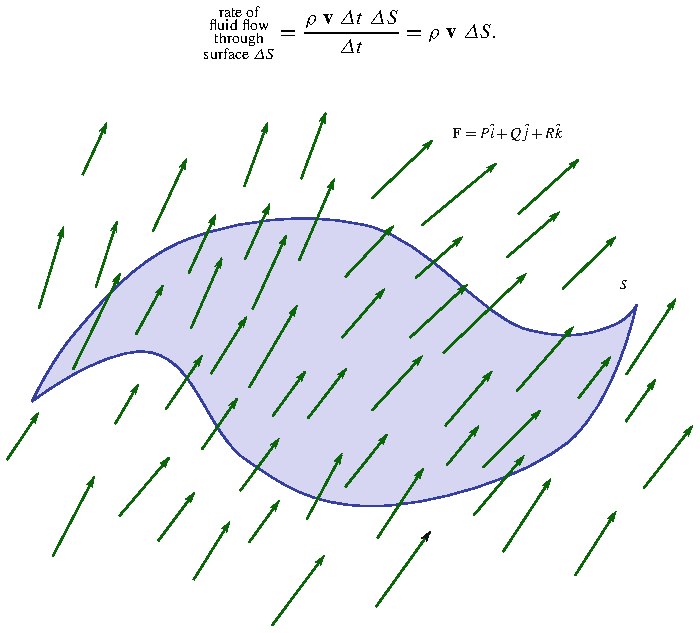
\includegraphics[width=0.832\linewidth]{images/vector/fig-9-1.pdf}
  \caption{$\mathbb{R}^3$ 中的向量场 $F=P\hat{\imath}+Q\hat{\jmath}+R\hat{k}$ 以及二维曲面 $S$}
  \label{fig:9-1}
\end{figure}

\begin{figure}[htbp]
  \centering
  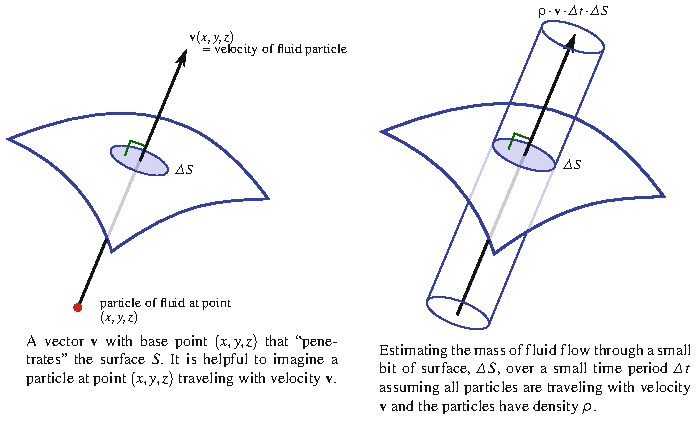
\includegraphics[width=0.827\linewidth]{images/vector/fig-9-2.pdf}
  \caption{把向量场 $v$ 在曲面 $S$ 上的积分想成求以速度 $v$ 运动并通过该曲面的流体的流率，是一种自然的思考方式}
  \label{fig:9-2}
\end{figure}

假设对于密度为 $\rho(x,y,z)$ 的某种流体，$v(x,y,z)$ 是点 $(x,y,z)$ 处的流体粒子的流动速度. 我们想求有多少流体流过某个小曲面 $\Delta S$. 如果我们假设 $v$ 垂直于 $\Delta S$，那么在一个小时间段 $\Delta t$ 内，流过 $\Delta S$ 的流体的质量由 $\rho(x,y,z)v(x,y,z)\Delta t\Delta S$ 给出，如图~\ref{fig:9-2} 所示. 流率由穿过曲面的流体质量除以这些质量穿过曲面的时间给出：
\[
\text{通过曲面 }\Delta S\text{ 的流体流率}=\frac{\rho v\Delta t\Delta S}{\Delta t}=\rho v\Delta S.
\]

如果 $v$ 不垂直于曲面 $\Delta S$，那么通过 $\Delta S$ 的流动由 $\rho(x,y,z)\,v(x,y,z)\cdot\hat{n}\,\Delta t\Delta S$ 给出. 也就是说，我们把乘积中的 $v$ 替换为 $v\cdot\hat{n}$，即与曲面元素 $\Delta S$ 的单位法向量的点积. 这个点积给出 $v$ 在 $\hat{n}$ 方向的分量. 见图~\ref{fig:9-3}. 换句话说，它给出流体在 $\hat{n}$ 方向的流动速度，
\[
\text{通过曲面 }\Delta S\text{ 的流体流率}=\frac{\rho(v\cdot\hat{n})\Delta t\Delta S}{\Delta t}=\rho(v\cdot\hat{n})\Delta S.
\]

\begin{figure}[htbp]
  \centering
  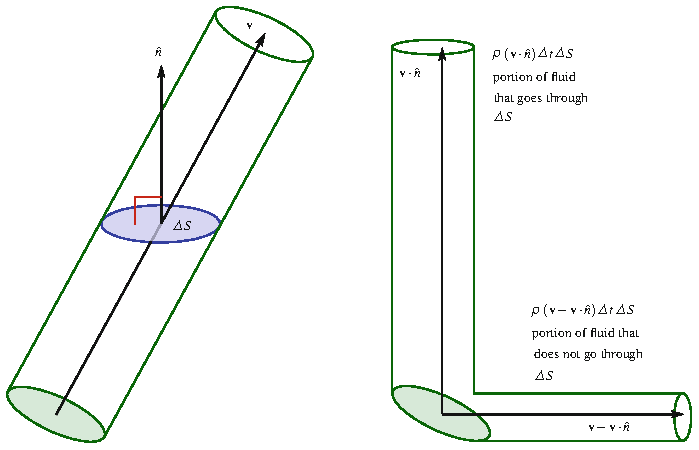
\includegraphics[width=0.960\linewidth]{images/vector/fig-9-3.pdf}
  \caption{假设 $v$ 不垂直于曲面 $S$（左）. 那么我们把流体流动``分解''成两部分：穿过曲面 $S$ 的那部分和不穿过 $S$ 的那部分（右）. 这需要取 $v$ 与 $S$ 的单位法向量（记为 $\hat{n}$）的点积}
  \label{fig:9-3}
\end{figure}

我们可以通过把 $S$ 分成小块 $\Delta S$、求每一块的流动然后求和，来近似整个曲面 $S$ 的流体流动. 然后为了求精确的流动，我们可以取 $\Delta S$ 的大小收缩到零的极限，即 $|\Delta S|\to0$：
\[
\text{流率}=\lim_{|\Delta S_i|\to0}\sum_i\rho(v\cdot\hat{n})\Delta S_i=\iint_S\rho(v\cdot\hat{n})\,dS.
\]

我们一直在处理一个具体的情形——流体流动——来帮助我们更好地理解正在发生的事情. 但同样的推理适用于任何向量场 $F$；我们可以求向量场 $F$ 穿过曲面 $S$ 的``流动''. 但是当我们拿掉流体这个心理拐杖、只处理向量场时，实际上没有流体密度 $\rho$，所以我们必须从上面的等式中去掉 $\rho$. 但在这种更纯粹的情形下，我们只有向量场而没有流体，我们实际上并不是在求流体流过 $S$ 的流率. 我们求的这个公认抽象的东西被称为向量场 $F$ 穿过曲面 $S$ 的\newterm{flux}{通量}{flux}. 通量（flux）是拉丁语中``流动''的意思. 通量在物理情形中实际代表什么取决于具体问题以及向量场被如何解释. 这个向量是流体流动？是电场？是磁场？是力？在每种情况下，穿过曲面的通量都会被不同地解释. 所以通量实际上是一个抽象数学概念，在不同的物理情形下可以被不同地解释. 稍后我们将看到场 $F$ 表示电场或磁场的例子，我们将求出穿过曲面的电通量和磁通量. 然而，一般来说，思考通量到底是什么的最好方法大概是想象一种没有密度的流体. 这样我们就有
\[
\operatorname{Flux}(F)=\lim_{|\Delta S_i|\to0}\sum_i F\cdot\hat{n}\,\Delta S_i=\iint_S F\cdot\hat{n}\,dS.
\]
注意这个积分有意义：在曲面 $S$ 上的每个点 $p$，$F_p\cdot\hat{n}_p$ 是一个实数. 也就是说，我们可以把 $F\cdot\hat{n}$ 想成 $S$ 上的实值函数，$F\cdot\hat{n}:S\to\mathbb{R}$，这意味着我们可以容易地把它在曲面 $S$ 上积分. 在向量微积分中你学过各种做这件事的技巧. 总之，向量场 $F$ 穿过曲面 $S$ 的通量由积分
\[
\operatorname{Flux}(F)=\iint_S F\cdot\hat{n}\,dS
\]
给出.

关于记号的两点说明：有时这个积分写成 $\oint_S F\cdot dS$ 或 $\iint_S F\cdot dS$. 所以当你看到 $\oint_S F\cdot dS$ 或 $\iint_S F\cdot dS$ 时，它的意思正是 $\iint_S F\cdot\hat{n}\,dS$. 这种记号将在第~\ref{sec:9-5-3}~小节中更深入地解释. 另外，由于 $S$ 是曲面而不是函数，显然 $dS$ 不代表一个 0-形式的外微分. 但 $dS$ 来自 $\Delta S$，它表示曲面 $S$ 的一小块的面积，所以粗略地你可以把 $dS$ 想成曲面 $S$ 上的一个``面积形式''，它允许你求出曲面 $S$ 的面积. 我们在这里不深入细节.

现在我们将定义 $F$ 在点 $(x_0,y_0,z_0)$ 处的散度. 假设我们有一个围绕点 $(x_0,y_0,z_0)$ 的小三维区域 $V$. 这个区域 $V$ 的边界记为 $\partial V$. 所谓闭的，我们的意思是曲面 $S$ 像一个没有边的球面. 我们还将区域 $V$ 的体积记为 $\Delta V$. 那么我们把 $F$ 的散度定义为
\begin{definition}[散度的定义]\label{def:9-1-1}
\[
\operatorname{div}F=\lim_{\Delta V\to0}\frac{1}{\Delta V}\oint_{\partial V}F\cdot\hat{n}\,dS.
\]
\end{definition}

理解这实际上代表什么可能会更容易一些，如果我们把右边写成
\[
\lim_{\Delta V\to0}\frac{\oint_{\partial V}F\cdot\hat{n}\,dS}{\Delta V}
\]
并考虑这意味着什么. 在分子中是穿过 $\partial V$ 的通量，即向量场穿过曲面 $\partial V$ 的流动. 由于 $\partial V$ 是闭曲面，如果我们选择法向量 $\hat{n}$ 指向外部，那么 $F$ 穿过 $\partial V$ 的通量就是 $F$ 流出 $V$ 的净通量减去流入 $V$ 的净通量. 换句话说，$F$ 通过 $\partial V$ 流出 $V$ 的净通量，即 $\oint_{\partial V}F\cdot\hat{n}\,dS$，可以是正的、零或负的. 把 $F$ 流出 $V$ 的净通量除以 $\Delta V$，我们求的是 $F$ 流出 $V$ 的每单位体积的净通量. 当我们让围绕点 $(x_0,y_0,z_0)$ 的体积 $\Delta V$ 的极限趋于零时，我们求出的就是在点 $(x_0,y_0,z_0)$ 处每单位体积的净流出通量. 换句话说，这就是向量场 $F$ 在点 $(x_0,y_0,z_0)$ 处``发散''的程度.

如果 $\operatorname{div}F$ 在点 $(x_0,y_0,z_0)$ 处为正，那么这意味着向量场 $F$ 正在从点 $(x_0,y_0,z_0)$ 向外发散. 如果 $\operatorname{div}F$ 在点 $(x_0,y_0,z_0)$ 处为负，那么这意味着向量场 $F$ 正在点 $(x_0,y_0,z_0)$ 处积聚. 如果 $\operatorname{div}F$ 在点 $(x_0,y_0,z_0)$ 处为零，那么 $F$ 在该点既不积聚也不发散. 见图~\ref{fig:9-4}.

\begin{figure}[htbp]
  \centering
  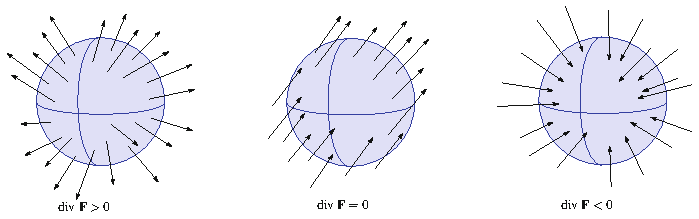
\includegraphics[width=0.960\linewidth]{images/vector/fig-9-4.pdf}
  \caption{向量场关于点 $(x_0,y_0,z_0)$ 周围小体积 $\Delta V$ 的通量的三个例子. 图中显示了通量为正（左）、为零（中）和为负（右）的情形}
  \label{fig:9-4}
\end{figure}

现在我们想用 $F$ 的散度的定义 $\operatorname{div}F=\lim_{\Delta V\to0}\frac{1}{\Delta V}\oint_{\partial V}F\cdot\hat{n}\,dS$ 来得到你在向量微积分中学过的散度标准公式 $\frac{\partial P}{\partial x}+\frac{\partial Q}{\partial y}+\frac{\partial R}{\partial z}$. 利用图~\ref{fig:9-5} 中所示的立方体区域 $V$，我们有曲面 $S_1$ 和 $S_2$，它们平行于 $y$ 轴和 $z$ 轴、垂直于 $x$ 轴. 我们把 $S_1$ 想成立方体的前面，把 $S_2$ 想成立方体的后面. $S_1$ 的朝外法向量是 $\hat{n}_{S_1}=\hat{\imath}$，$S_2$ 的朝外法向量是 $\hat{n}_{S_2}=-\hat{\imath}$. 我们有
\[
\oint_{S_1}F\cdot\hat{n}_{S_1}\,dS\approx F\Bigl(x_0+\frac{\Delta x}{2},y_0,z_0\Bigr)\cdot\hat{\imath}\,\Delta y\Delta z=P\Bigl(x_0+\frac{\Delta x}{2},y_0,z_0\Bigr)\Delta y\Delta z
\]
和
\[
\oint_{S_2}F\cdot\hat{n}_{S_2}\,dS\approx F\Bigl(x_0-\frac{\Delta x}{2},y_0,z_0\Bigr)\cdot(-\hat{\imath})\,\Delta y\Delta z=-P\Bigl(x_0-\frac{\Delta x}{2},y_0,z_0\Bigr)\Delta y\Delta z.
\]

\begin{figure}[htbp]
  \centering
  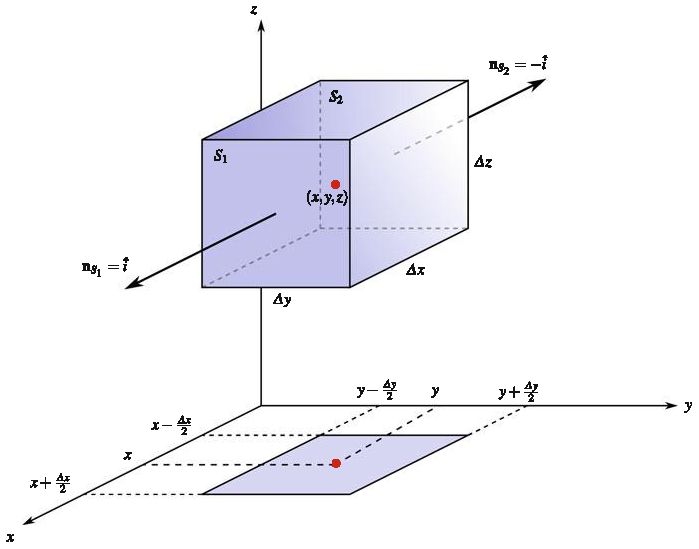
\includegraphics[width=0.960\linewidth]{images/vector/fig-9-5.pdf}
  \caption{区域 $V$ 是边长分别为 $\Delta x$、$\Delta y$ 和 $\Delta z$ 的立方体，因此 $\Delta V=\Delta x\Delta y\Delta z$. 侧面 $S_1$ 和 $S_2$（立方体的前面和后面）垂直于 $x$ 轴. $S_1$ 的朝外单位法向量是 $\hat{\imath}$，$S_2$ 的朝外单位法向量是 $-\hat{\imath}$}
  \label{fig:9-5}
\end{figure}

求和得到
\begin{align*}
\oint_{S_1+S_2}F\cdot\hat{n}\,dS\approx\Bigl[P\Bigl(x_0+\frac{\Delta x}{2},y_0,z_0\Bigr)-P\Bigl(x_0-\frac{\Delta x}{2},y_0,z_0\Bigr)\Bigr]\Delta y\Delta z \\
=\frac{P\bigl(x_0+\frac{\Delta x}{2},y_0,z_0\bigr)-P\bigl(x_0-\frac{\Delta x}{2},y_0,z_0\bigr)}{\Delta x}\Delta x\Delta y\Delta z, \\
\Rightarrow\quad\frac{1}{\Delta x\Delta y\Delta z}\oint_{S_1+S_2}F\cdot\hat{n}\,dS\approx\frac{P\bigl(x_0+\frac{\Delta x}{2},y_0,z_0\bigr)-P\bigl(x_0-\frac{\Delta x}{2},y_0,z_0\bigr)}{\Delta x}.
\end{align*}
回想 $\Delta V=\Delta x\Delta y\Delta z$，然后取 $\Delta V\to0$（即 $\Delta x\to0$、$\Delta y\to0$ 和 $\Delta z\to0$）的极限，我们得到
\begin{align*}
\lim_{\Delta V\to0}\frac{1}{\Delta V}\oint_{S_1+S_2}F\cdot\hat{n}\,dS
=\lim_{\Delta V\to0}\frac{P\bigl(x_0+\frac{\Delta x}{2},y_0,z_0\bigr)-P\bigl(x_0-\frac{\Delta x}{2},y_0,z_0\bigr)}{\Delta x} \\
=\lim_{\Delta x\to0}\frac{P\bigl(x_0+\frac{\Delta x}{2},y_0,z_0\bigr)-P\bigl(x_0-\frac{\Delta x}{2},y_0,z_0\bigr)}{\Delta x}
=\left.\frac{\partial P}{\partial x}\right|_{(x_0,y_0,z_0)}.
\end{align*}
在极限中近似变成等式. 另外，由于右边没有 $\Delta y$ 或 $\Delta z$，$\Delta V\to0$ 就简化为 $\Delta x\to0$.

\begin{question}\label{q:9-1}
令 $S_3$ 和 $S_4$ 是区域 $V$ 中垂直于 $y$ 轴的侧面，即立方体的右侧面和左侧面. 令 $S_5$ 和 $S_6$ 是垂直于 $z$ 轴的侧面，即立方体的顶面和底面. 对曲面 $S_3+S_4$ 和 $S_5+S_6$ 重复这些计算，得到
\[
\lim_{\Delta V\to0}\frac{1}{\Delta V}\oint_{S_3+S_4}F\cdot\hat{n}\,dS=\left.\frac{\partial Q}{\partial y}\right|_{(x_0,y_0,z_0)},\qquad
\lim_{\Delta V\to0}\frac{1}{\Delta V}\oint_{S_5+S_6}F\cdot\hat{n}\,dS=\left.\frac{\partial R}{\partial z}\right|_{(x_0,y_0,z_0)}.
\]
\end{question}

把所有项加在一起，我们有
\begin{align*}
\operatorname{div}F=\lim_{\Delta V\to0}\frac{1}{\Delta V}\oint_{\partial V}F\cdot\hat{n}\,dS
=\lim_{\Delta V\to0}\frac{1}{\Delta V}\oint_{S_1+S_2+S_3+S_4+S_5+S_6}F\cdot\hat{n}\,dS \\
=\left.\frac{\partial P}{\partial x}\right|_{(x_0,y_0,z_0)}+\left.\frac{\partial Q}{\partial y}\right|_{(x_0,y_0,z_0)}+\left.\frac{\partial R}{\partial z}\right|_{(x_0,y_0,z_0)}
=\frac{\partial P}{\partial x}+\frac{\partial Q}{\partial y}+\frac{\partial R}{\partial z}.
\end{align*}
换句话说，我们刚刚找到了下面的公式：
\begin{theorem}[散度的计算公式（笛卡尔坐标）]\label{thm:9-1}
\[
\operatorname{div}F=\frac{\partial P}{\partial x}+\frac{\partial Q}{\partial y}+\frac{\partial R}{\partial z}.
\]
\end{theorem}

由于我们可以在任何一点取散度，记号中通常略去点. 我们用 $\nabla\cdot F$ 作为记忆辅助手段来帮助记住这个公式.

现在我们来看向量微积分中的散度定理（有时称为 Gauss 定理）. 我们将（以非常不严格的方式）``推导''散度定理. 鉴于我们定义 $\operatorname{div}F$ 的方式，这是相当直截了当的. 我们将利用这样的事实：穿过曲面 $S$ 的通量是穿过 $S$ 的各子曲面 $S_i$ 的通量之和，
\[
\oint_S F\cdot\hat{n}\,dS=\sum_i\oint_{S_i}F\cdot\hat{n}\,dS.
\]
为了理解这一点，考虑图~\ref{fig:9-6} 中所示的两个共享公共表面 $S_c$ 的相邻体积 $V_1$ 和 $V_2$. $V_1$ 的表面 $S_c$ 具有朝外法向量 $\hat{n}_1$，而 $V_2$ 的表面 $S_c$ 具有朝外法向量 $\hat{n}_2$. 显然 $\hat{n}_2=-\hat{n}_1$. 从图~\ref{fig:9-6} 中很容易看出
\[
\oint_{S_c}F\cdot\hat{n}_1\,dS+\oint_{S_c}F\cdot\hat{n}_2\,dS=\oint_{S_c}F\cdot\hat{n}_1\,dS-\oint_{S_c}F\cdot\hat{n}_1\,dS=0.
\]

\begin{figure}[htbp]
  \centering
  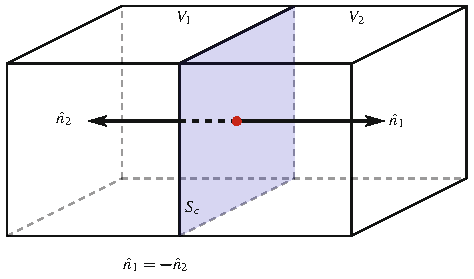
\includegraphics[width=0.562\linewidth]{images/vector/fig-9-6.pdf}
  \caption{共享公共表面 $S_c$ 的两个相邻的立方体积 $V_1$ 和 $V_2$. $V_1$ 的表面 $S_c$ 具有朝外法向量 $\hat{n}_1$，而 $V_2$ 的表面 $S_c$ 具有朝外法向量 $\hat{n}_2$，其中 $\hat{n}_2=-\hat{n}_1$}
  \label{fig:9-6}
\end{figure}

给定一个带曲面 $\partial V$ 的大体积 $V$，如图~\ref{fig:9-7} 所示，它可以被细分为 $N$ 个更小的体积 $V_i$. 此外，这些小体积所有内部表面的通量彼此抵消，
\[
\oint_{\partial V}F\cdot\hat{n}\,dS\approx\sum_{i=1}^{N}\frac{1}{\Delta V_i}\oint_{S_i}F\cdot\hat{n}\,dS\ \Delta V_i=\sum_{i=1}^{N}(\operatorname{div}F)_i\Delta V_i.
\]
当我们取 $N\to\infty$ 且 $|\Delta V_i|\to0$ 的极限时，由于内部表面全部抵消，$\sum V_i\to V$ 且 $\sum\partial V_i\to\partial V$. 所以当我们取极限时，得到下面的等式：
\[
\oint_{\partial V}F\cdot\hat{n}\,dS=\lim_{\substack{N\to\infty\\|\Delta V_i|\to0}}\sum_{i=1}^{N}(\operatorname{div}F)_i\Delta V_i=\iiint_V\operatorname{div}F\,dV,
\]

\begin{figure}[htbp]
  \centering
  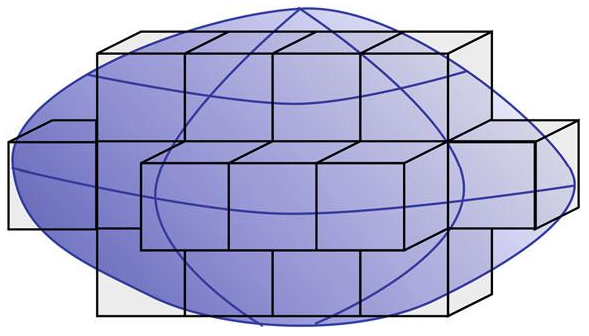
\includegraphics[width=0.815\linewidth]{images/vector/fig-9-7.pdf}
  \caption{被较小的立方体积 $V_i$ 覆盖的不规则形状的体积 $V$. 当 $\Delta V_i\to0$ 时，不规则形状的体积被逼近得越来越好}
  \label{fig:9-7}
\end{figure}

这正是散度定理. 回想 $V$ 的边界是 $\partial V=S$，并把 $F\cdot dS$ 写成 $F\cdot\hat{n}\,dS$，散度定理通常写成
\begin{theorem}[散度定理]\label{thm:9-2}
\[
\oint_{\partial V}F\cdot dS=\iiint_V\operatorname{div}F\,dV.
\]
\end{theorem}

在本节中，我们使用了 $\mathbb{R}^3$ 上用笛卡尔坐标书写的向量场 $F$ 的散度定义，求出了 $\operatorname{div}F$ 的表达式. 但笛卡尔坐标并不是 $\mathbb{R}^3$ 上唯一的坐标系. 第 6.5 节中引入的柱坐标系和球坐标系也是 $\mathbb{R}^3$ 上非常常用的坐标系.

\begin{question}\label{q:9-2}
假设 $F=F_r\hat{e}_r+F_\theta\hat{e}_\theta+F_z\hat{e}_z$ 是关于柱坐标书写的 $\mathbb{R}^3$ 上的向量场. 向量 $\hat{e}_r$ 是 $r$ 增大方向的单位向量，$\hat{e}_\theta$ 是 $\theta$ 增大方向的单位向量，$\hat{e}_z$ 是 $z$ 增大方向的单位向量. 利用图~\ref{fig:6-14} 中所示的柱坐标体积元素和与本节类似的过程，证明
\[
\operatorname{div}F=\frac{1}{r}\frac{\partial(rF_r)}{\partial r}+\frac{1}{r}\frac{\partial F_\theta}{\partial\theta}+\frac{\partial F_z}{\partial z}.
\]
\end{question}

\begin{question}\label{q:9-3}
假设 $F=F_r\hat{e}_r+F_\theta\hat{e}_\theta+F_\varphi\hat{e}_\varphi$ 是关于球坐标书写的 $\mathbb{R}^3$ 上的向量场. 向量 $\hat{e}_r$ 是 $r$ 增大方向的单位向量，$\hat{e}_\theta$ 是 $\theta$ 增大方向的单位向量，$\hat{e}_\varphi$ 是 $\varphi$ 增大方向的单位向量. 利用图~\ref{fig:6-16} 中所示的球坐标体积元素和与本节类似的过程，证明
\[
\operatorname{div}F=\frac{1}{r^2}\frac{\partial(r^2F_r)}{\partial r}+\frac{1}{r\sin\theta}\frac{\partial(\sin\theta\,F_\theta)}{\partial\theta}+\frac{1}{r\sin\theta}\frac{\partial F_\varphi}{\partial\varphi}.
\]
\end{question}

\section{旋度}

给定一个向量场 $F=P\hat{\imath}+Q\hat{\jmath}+R\hat{k}$，在向量微积分课程中，向量场的旋度通常定义为
\[
\operatorname{curl}F=\Bigl(\frac{\partial R}{\partial y}-\frac{\partial Q}{\partial z}\Bigr)\hat{\imath}+\Bigl(\frac{\partial P}{\partial z}-\frac{\partial R}{\partial x}\Bigr)\hat{\jmath}+\Bigl(\frac{\partial Q}{\partial x}-\frac{\partial P}{\partial y}\Bigr)\hat{k}.
\]
常常你还会看到这样的写法：
\[
\operatorname{curl}F=\nabla\times F,
\]
其中 $\nabla$ 就是前面定义的算子
\[
\nabla=\frac{\partial}{\partial x}\hat{\imath}+\frac{\partial}{\partial y}\hat{\jmath}+\frac{\partial}{\partial z}\hat{k},
\]
并且使用了记住两个向量``叉积''$\times$ 的常用记忆辅助手段：
\[
\nabla\times F=\begin{vmatrix}
\hat{\imath}&\hat{\jmath}&\hat{k}\\[2pt]
\dfrac{\partial}{\partial x}&\dfrac{\partial}{\partial y}&\dfrac{\partial}{\partial z}\\[2pt]
P&Q&R
\end{vmatrix}.
\]
重要的是要认识到，$\nabla\times F$ 的这种表述实际上只不过是一种记忆辅助手段，帮助我们重构 $\operatorname{curl}F$ 的公式，假设我们记得如何取 $3\times3$ 矩阵的行列式. 再次，和散度的情况一样，我们将采取稍微不同的方法，以更几何的方式定义旋度，使得 $\operatorname{curl}F$ 的公式和 Stokes 定理都能直接落出来. 然而，在我们真正做出这个定义之前，我们需要理解一些必要的背景材料.

我们从考虑点积的几何意义开始：
\[
v\cdot w=|v|\,|w|\cos\theta,
\]
如图~\ref{fig:9-8} 所示. 如果 $|v|=1$，即 $v$ 是单位向量，那么 $v\cdot w=|w|\cos\theta$，这是 $w$ 指向 $v$ 方向的分量. 现在假设我们想以某种方式度量向量场 $F$ 在某个曲线 $C$ 方向上的``分量''. 我们可以用刚定义的点积来求出它，见图~\ref{fig:9-10}. 之后我们将想要对我们求出的这个``分量''积分.

\begin{figure}[htbp]
  \centering
  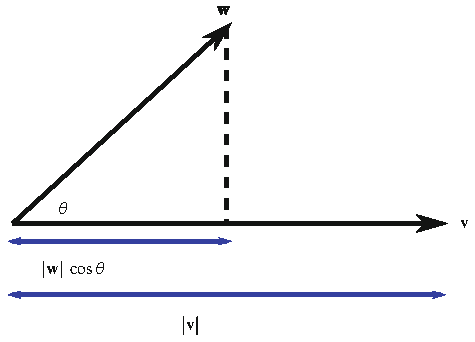
\includegraphics[width=0.563\linewidth]{images/vector/fig-9-8.pdf}
  \caption{点积的几何意义 $v\cdot w=|v|\,|w|\cos\theta$.}
  \label{fig:9-8}
\end{figure}

然而，我们首先需要理解向量场的线积分. 同样，我们假设你上过向量微积分课程，所以我们介绍这些材料时不作太多细节. 不过，我们需要做一个记号的说明以帮助你避免混淆. 我们将围绕闭曲线积分，用 $C$ 表示闭曲线. 这些闭曲线将由弧长参数化，我们用小写字母 $s$ 表示弧长. 我们用大写字母 $S$ 表示边界为曲线 $C$ 的曲面，即 $C=\partial S$. 如果曲线 $C$ 位于一个平面内，我们假定曲面 $S$ 也位于该平面内. 如果是这种情况，那么曲面 $S$ 的单位法向量记为 $\hat{n}$. 为让生活更简单，我们在下文中就假定这种情况.

假设曲线 $C$ 由弧长参数化. 曲线 $C$ 上的点 $s$ 的坐标为 $x=x(s)$、$y=y(s)$、$z=z(s)$，点 $s+\Delta s$ 的坐标为 $x+\Delta x=x(s+\Delta s)$、$y+\Delta y=y(s+\Delta s)$、$z+\Delta z=z(s+\Delta s)$，由此给出
\[
\Delta x=x(s+\Delta s)-x(s),\qquad
\Delta y=y(s+\Delta s)-y(s),\qquad
\Delta z=z(s+\Delta s)-z(s).
\]
令 $\Delta r$ 是从点 $\bigl(x(s),y(s),z(s)\bigr)$ 到点 $\bigl(x(s+\Delta s),y(s+\Delta s),z(s+\Delta s)\bigr)$ 的向量，我们有
\[
\frac{\Delta r}{\Delta s}=\frac{\Delta x}{\Delta s}\hat{\imath}+\frac{\Delta y}{\Delta s}\hat{\jmath}+\frac{\Delta z}{\Delta s}\hat{k}.
\]
我们通过取右边当 $\Delta s\to0$ 时的极限来定义新的向量 $\hat{t}$，这当然也意味着 $\Delta x,\Delta y,\Delta z\to0$：
\[
\hat{t}=\lim_{\Delta s\to0}\Bigl(\frac{\Delta x}{\Delta s}\hat{\imath}+\frac{\Delta y}{\Delta s}\hat{\jmath}+\frac{\Delta z}{\Delta s}\hat{k}\Bigr)=\frac{dx}{ds}\hat{\imath}+\frac{dy}{ds}\hat{\jmath}+\frac{dz}{ds}\hat{k}.
\]

\begin{figure}[htbp]
  \centering
  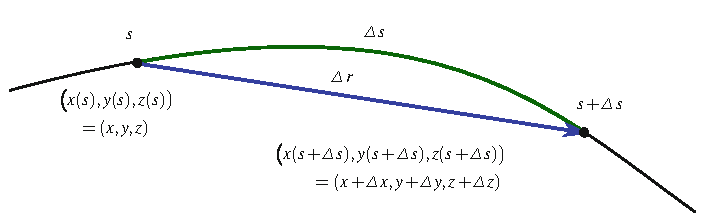
\includegraphics[width=0.840\linewidth]{images/vector/fig-9-9.pdf}
  \caption{曲线的单位切向量 $\hat{t}$ 是 $\Delta r/\Delta s=\frac{\Delta x}{\Delta s}\hat{\imath}+\frac{\Delta y}{\Delta s}\hat{\jmath}+\frac{\Delta z}{\Delta s}\hat{k}$ 的极限}
  \label{fig:9-9}
\end{figure}

从图~\ref{fig:9-9} 可以看出，$\hat{t}$ 是曲线 $C$ 的切向量. 此外，当 $\Delta s\to0$ 时容易看出 $|\Delta r|\to\Delta s$. 因此 $|\hat{t}|=1$，所以 $\hat{t}$ 是曲线 $C$ 的\newterm{unit-tangent-vector}{单位切向量}{unit tangent vector}. 另外，注意形式上我们可以写 $\hat{t}\,ds=\hat{\imath}dx+\hat{\jmath}dy+\hat{k}dz$，我们把它定义为 $ds$.

现在我们转向向量场 $F=P\hat{\imath}+Q\hat{\jmath}+R\hat{k}$ 沿曲线 $C$（由弧长 $s$ 参数化）的线积分. 沿曲线 $C$ 的方向的 $F$ 的分量由 $F\cdot\hat{t}$ 给出，其中 $\hat{t}$ 是 $C$ 的单位切向量. 见图~\ref{fig:9-10} 和图~\ref{fig:9-11}. 假设我们把曲线 $C$ 分成小段，每段长度为 $\Delta s$. 那么每一段上沿 $C$ 方向的 $F$ 的分量可以近似为 $(F\cdot\hat{t})\Delta s$：
\[
(F\cdot\hat{t})\Delta s=\Bigl(P\hat{\imath}+Q\hat{\jmath}+R\hat{k}\Bigr)\cdot\Bigl(\frac{\Delta x}{\Delta s}\hat{\imath}+\frac{\Delta y}{\Delta s}\hat{\jmath}+\frac{\Delta z}{\Delta s}\hat{k}\Bigr)\Delta s
=\Bigl(P\frac{\Delta x}{\Delta s}+Q\frac{\Delta y}{\Delta s}+R\frac{\Delta z}{\Delta s}\Bigr)\Delta s.
\]

\begin{figure}[htbp]
  \centering
  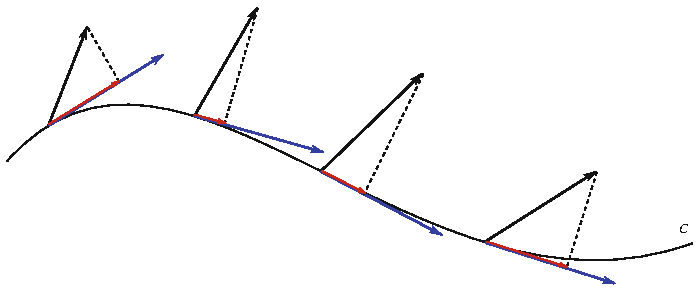
\includegraphics[width=0.958\linewidth]{images/vector/fig-9-10.pdf}
  \caption{向量场 $F$（黑色）定义在曲线 $C$ 上. 我们想知道 $F$ 与 $C$ 相切的那``部分''. 为此我们考虑 $C$ 的单位切向量 $\hat{t}$（蓝色），并求 $F\cdot\hat{t}$（红色），以找出 $F$ 指向 $\hat{t}$ 方向、从而与曲线 $C$ 相切的那``部分''. 我们在曲线 $C$ 的每一点都这样做. 另见图~\ref{fig:9-11}}
  \label{fig:9-10}
\end{figure}

\begin{figure}[htbp]
  \centering
  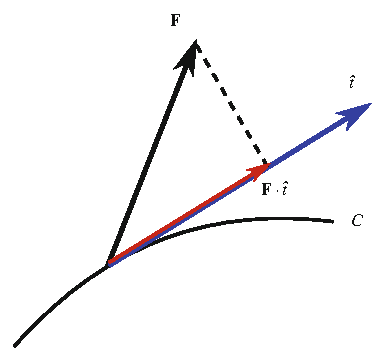
\includegraphics[width=0.452\linewidth]{images/vector/fig-9-11.pdf}
  \caption{图~\ref{fig:9-10} 中一段的放大图. 我们想知道 $F$ 与 $C$ 相切的那``部分''. 为此我们考虑 $C$ 的单位切向量 $\hat{t}$（蓝色），并求 $F\cdot\hat{t}$（红色），以找出 $F$ 指向 $\hat{t}$ 方向、从而与曲线 $C$ 相切的那``部分''}
  \label{fig:9-11}
\end{figure}

所以我们得到
\[
\int_C F\cdot\hat{t}\,ds=\lim_{|\Delta s|\to0}\sum\Bigl(P\frac{\Delta x}{\Delta s}+Q\frac{\Delta y}{\Delta s}+R\frac{\Delta z}{\Delta s}\Bigr)\Delta s.
\]
利用上一段中的记号，积分 $\int_C F\cdot\hat{t}\,ds$ 也可以写成 $\int_C F\cdot ds$.

现在我们知道了沿曲线积分向量场意味着什么，就可以准备定义 $\operatorname{curl}F$ 在点 $(x_0,y_0,z_0)$ 处的值了：
\begin{definition}[旋度的定义]\label{def:9-2-1}
\[
\hat{n}\cdot\operatorname{curl}F=\lim_{|\Delta S|\to0}\frac{1}{\Delta S}\oint_C F\cdot\hat{t}\,ds,
\]
其中 $S$ 是以闭曲线 $C=\partial S$ 为边界的曲面，$\Delta S$ 是该曲面的面积，$\hat{n}$ 是该曲面的单位法向量，$ds$ 中的 $s$ 是无穷小弧长元素，曲面面积 $\Delta S$ 围绕点 $(x_0,y_0,z_0)$ 收缩到零.
\end{definition}

回忆，法向量与曲面 $S$ 所在平面正交，即与之成直角. 曲线 $C$、$F$ 以及 $F$ 沿曲线的分量显示在图~\ref{fig:9-12} 中. 对这个积分积分、除以 $\Delta S$，然后取 $\Delta S\to0$ 的极限，就给出 $\operatorname{curl}F$ 定义右边的值. 本质上，旋度是向量场 $F$ 绕某点无穷小路径的每单位面积的``环流''.

\begin{figure}[htbp]
  \centering
  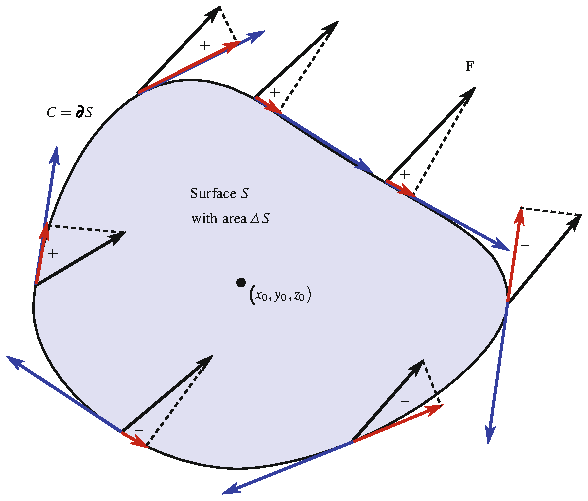
\includegraphics[width=0.720\linewidth]{images/vector/fig-9-12.pdf}
  \caption{图中显示了沿闭曲线 $C$ 的向量场 $F$（黑色）. 图中显示了 $C$ 的单位切向量（蓝色）以及 $F$ 沿 $C$ 的``部分''（红色）. 注意，有时 $F$ 沿 $C$ 的``部分''为正，有时为负}
  \label{fig:9-12}
\end{figure}

\begin{question}\label{q:9-4}
利用图~\ref{fig:9-12} 和如图所示的向量场 $F$，根据积分定义为 $(F\cdot\hat{t})\Delta s$ 之和的极限，估计 $\oint_C F\cdot\hat{t}\,ds$. 换句话说，这个积分是大的还是小的、正的还是负的数，还是接近于零？根据积分的定义解释你的答案.
\end{question}

\begin{question}\label{q:9-5}
画一个像图~\ref{fig:9-12} 那样的图，其中向量场 $F$ 围绕 $(x_0,y_0,z_0)$ 逆时针旋转. 假设 $C$ 的切向量也是逆时针方向的. 积分 $\oint_C F\cdot\hat{t}\,ds$ 是大的还是小的、正的还是负的数，还是接近于零？利用图和积分的定义方式解释为什么. 对顺时针旋转的向量场 $F$ 重复上述过程.
\end{question}

我们想尽力理解这个古怪的定义. 希望最后两个问题已经说明，我们是在试图度量向量场 $F$ 是如何围绕某点``旋转''的. 当我们取 $|\Delta S|\to0$ 的极限时，得到的是点 $(x_0,y_0,z_0)$ 处每单位面积的环流. 但注意定义的左边，$\operatorname{curl}F$ 与曲面 $S$ 的单位法向量 $\hat{n}$ 点积，这告诉我们 $\operatorname{curl}F$ 本身一定是一个向量.

使这个定义有点棘手的问题是，在 $\mathbb{R}^3$ 中，有无数个平面通过点 $(x_0,y_0,z_0)$，因此有无数个可能的曲面 $S$ 及其对应的边界 $\partial S=C$，它们都可以围绕点 $(x_0,y_0,z_0)$ 收缩到面积为零. 也就是说，这本质上就是为什么旋度的定义这么古怪、需要点积的原因. 这个定义必须对通过 $(x_0,y_0,z_0)$ 的每个可能的平面以及该平面内围绕 $(x_0,y_0,z_0)$ 收缩到面积为零的每个可能的曲面 $S$ 都成立. 左边 $\hat{n}$（曲面 $S$ 的单位法向量）与 $\operatorname{curl}F$ 的点积，对应于（或者说补偿了）在右边选择某个放置曲面 $S$ 和曲线 $C$ 的特定平面.

让我们花几分钟更深入地探索一下. 考虑图~\ref{fig:9-13}，其中显示了围绕点 $(x_0,y_0,z_0)$ 的、边界为 $\partial S=C$ 的曲面 $S$. 沿 $C$ 的几个点处，曲线 $C$ 的单位切向量 $\hat{t}$ 用蓝色显示，在这些相同点处向量场 $F$ 用黑色显示. 每个场向量在 $\hat{t}$ 方向的分量显示为红色的 $F\cdot\hat{t}$，并且也标出了它的符号：如果 $F\cdot\hat{t}$ 指向 $\hat{t}$ 方向则为正，如果 $F\cdot\hat{t}$ 指向 $-\hat{t}$ 方向则为负. 我们把向量场 $F$ 中的所有向量都画成互相平行，以表明点 $(x_0,y_0,z_0)$ 周围没有环流发生. 这意味着正的 $F\cdot\hat{t}$ 的``量''与负的 $F\cdot\hat{t}$ 的``量''完全相同，导致 $\oint_C F\cdot\hat{t}\,ds=0$. 图中还显示了在点 $(x_0,y_0,z_0)$ 处画出的曲面 $S$ 的单位法向量 $\hat{n}$. 我们画 $\hat{n}$ 时让它相对于单位切向量 $\hat{t}$（蓝色）遵循右手法则. 我们这样做只是为了在不同曲面之间标准化 $F\cdot\hat{t}$ 的正负. 利用我们的旋度定义，我们有
\[
\hat{n}\cdot\operatorname{curl}F=\lim_{|\Delta S|\to0}\frac{1}{\Delta S}\oint_C F\cdot\hat{t}\,ds=0.
\]

\begin{figure}[htbp]
  \centering
  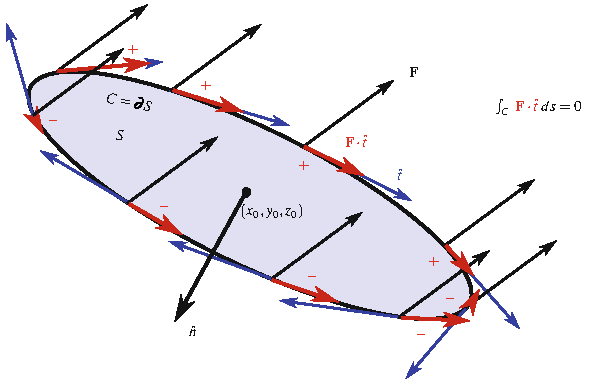
\includegraphics[width=0.720\linewidth]{images/vector/fig-9-13.pdf}
  \caption{$\hat{n}\cdot\operatorname{curl}F=0$ 的示意图. 我们画出了 $\operatorname{curl}F$ 定义中出现的所有分量，但向量 $\operatorname{curl}F$ 本身除外}
  \label{fig:9-13}
\end{figure}

所以，虽然我们可能实际上还不知道向量 $\operatorname{curl}F$ 是什么，但我们知道它必须垂直于 $\hat{n}$，因为 $\hat{n}\cdot\operatorname{curl}F=0$.

现在考虑图~\ref{fig:9-14}，其中几乎所有内容都与上一图相同，只是这次向量场 $F$ 的向量在某种意义上围绕点 $(x_0,y_0,z_0)$ 旋转. 注意现在所有的 $F\cdot\hat{t}$ 都指向与 $\hat{t}$ 相同的方向，因此都是正的. 这意味着
\[
\hat{n}\cdot\operatorname{curl}F=\lim_{|\Delta S|\to0}\frac{1}{\Delta S}\oint_C F\cdot\hat{t}\,ds>0.
\]

\begin{figure}[htbp]
  \centering
  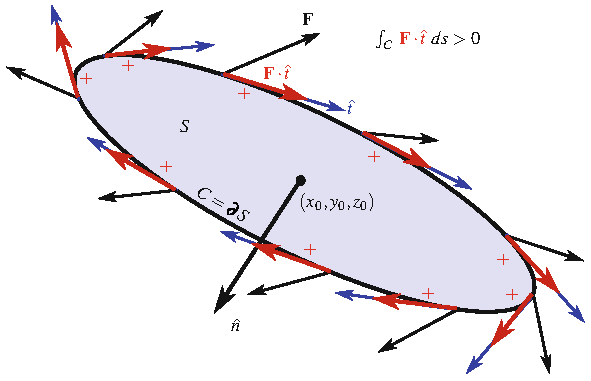
\includegraphics[width=0.700\linewidth]{images/vector/fig-9-14.pdf}
  \caption{$\hat{n}\cdot\operatorname{curl}F>0$ 的示意图. 同样我们画出了 $\operatorname{curl}F$ 定义中出现的所有分量，但向量 $\operatorname{curl}F$ 本身除外}
  \label{fig:9-14}
\end{figure}

所以，再次地，虽然我们可能实际上还不知道向量 $\operatorname{curl}F$ 是什么，但我们知道它与 $\hat{n}$ 点积时为正.

所以，实际求出向量 $\operatorname{curl}F$ 是什么，需要我们仔细地选择曲面及其对应的法向量. 显然，任何向量，包括向量 $\operatorname{curl}F$，都是欧几里得单位向量 $\hat{\imath}$、$\hat{\jmath}$ 和 $\hat{k}$ 的线性组合. 为了求出 $\operatorname{curl}F$ 中沿 $\hat{\imath}$ 方向的分量，我们需要求 $\operatorname{curl}F\cdot\hat{\imath}$. 类似地，为了求出 $\operatorname{curl}F$ 中沿 $\hat{\jmath}$ 方向的分量，我们需要求 $\operatorname{curl}F\cdot\hat{\jmath}$，为了求出 $\operatorname{curl}F$ 中沿 $\hat{k}$ 方向的分量，我们需要求 $\operatorname{curl}F\cdot\hat{k}$. 所以通过选择平行于 $yz$ 平面的 $S$，我们得到 $\hat{n}=\hat{\imath}$，这让我们能求出 $\operatorname{curl}F$ 的 $\hat{\imath}$ 项. 类似地，选择平行于 $xz$ 平面的 $S$ 给出 $\hat{n}=\hat{\jmath}$，这让我们能求出 $\operatorname{curl}F$ 的 $\hat{\jmath}$ 项，而选择平行于 $xy$ 平面的 $S$ 给出 $\hat{n}=\hat{k}$，这让我们能求出 $\operatorname{curl}F$ 的 $\hat{k}$ 项.

我们从选择平行于 $xy$ 平面（单位法向量为 $\hat{k}$）的平面内、围绕点 $(x_0,y_0,z_0)$ 的一条路径开始. 任何路径都可以，为简单起见我们选择图~\ref{fig:9-15} 中所示的正方形路径. 从上方俯视这条路径，我们可以把曲线的上、下、左、右边标为 $C_T$、$C_B$、$C_L$ 和 $C_R$，如图所示.

\begin{figure}[htbp]
  \centering
  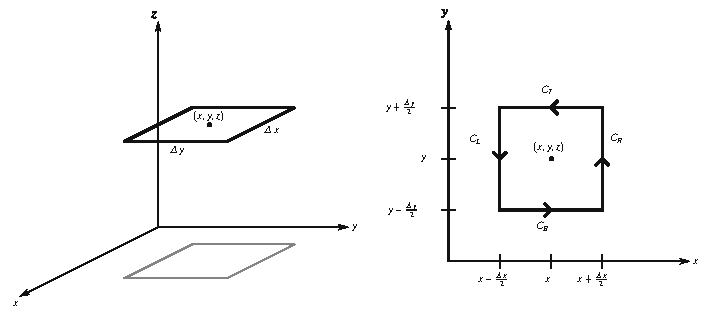
\includegraphics[width=0.960\linewidth]{images/vector/fig-9-15.pdf}
  \caption{围绕点 $(x,y,z)$ 的正方形曲线. 这条曲线位于平行于 $xy$ 平面的平面内（左），该平面具有单位法向量 $\hat{k}$. 从上方俯视同一条正方形曲线（右）. 这条正方形曲线由四条线段 $C_T$、$C_B$、$C_L$ 和 $C_R$ 组成}
  \label{fig:9-15}
\end{figure}

沿 $C_B$，单位切向量是 $\hat{t}=\hat{\imath}$，它给出 $F\cdot\hat{t}=F\cdot\hat{\imath}=P$. 所以我们有
\[
\oint_{C_B}F\cdot\hat{t}\,ds=\int_{C_B}P\,ds\approx P\Bigl(x_0,y_0-\frac{\Delta y}{2},z_0\Bigr)\Delta x.
\]
沿 $C_T$，单位切向量是 $\hat{t}=-\hat{\imath}$，它给出 $F\cdot\hat{t}=F\cdot(-\hat{\imath})=-P$. 所以我们有
\[
\oint_{C_T}F\cdot\hat{t}\,ds=\int_{C_T}-P\,ds\approx -P\Bigl(x_0,y_0+\frac{\Delta y}{2},z_0\Bigr)\Delta x.
\]
合在一起有
\begin{align*}
\oint_{C_T+C_B}F\cdot\hat{t}\,ds=-\frac{P\bigl(x_0,y_0+\frac{\Delta y}{2},z_0\bigr)-P\bigl(x_0,y_0-\frac{\Delta y}{2},z_0\bigr)}{\Delta y}\Delta x\Delta y, \\
\Rightarrow\quad\lim_{|\Delta S|\to0}\frac{1}{\Delta S}\oint_{C_T+C_B}F\cdot\hat{t}\,ds
=\lim_{\Delta y\to0}-\frac{P\bigl(x_0,y_0+\frac{\Delta y}{2},z_0\bigr)-P\bigl(x_0,y_0-\frac{\Delta y}{2},z_0\bigr)}{\Delta y}
=-\frac{\partial P}{\partial y}.
\end{align*}
沿 $C_R$，单位切向量是 $\hat{t}=\hat{\jmath}$，它给出 $F\cdot\hat{t}=F\cdot\hat{\jmath}=Q$. 所以我们有
\[
\oint_{C_R}F\cdot\hat{t}\,ds=\int_{C_R}Q\,ds\approx Q\Bigl(x_0+\frac{\Delta x}{2},y_0,z_0\Bigr)\Delta y.
\]
沿 $C_L$，单位切向量是 $\hat{t}=-\hat{\jmath}$，它给出 $F\cdot\hat{t}=F\cdot(-\hat{\jmath})=-Q$. 所以我们有
\[
\oint_{C_L}F\cdot\hat{t}\,ds=\int_{C_L}-Q\,ds\approx -Q\Bigl(x_0-\frac{\Delta x}{2},y_0,z_0\Bigr)\Delta y.
\]
合在一起有
\begin{align*}
\oint_{C_R+C_L}F\cdot\hat{t}\,ds=\frac{Q\bigl(x_0+\frac{\Delta x}{2},y_0,z_0\bigr)-Q\bigl(x_0-\frac{\Delta x}{2},y_0,z_0\bigr)}{\Delta x}\Delta x\Delta y, \\
\Rightarrow\quad\lim_{|\Delta S|\to0}\frac{1}{\Delta S}\oint_{C_R+C_L}F\cdot\hat{t}\,ds
=\lim_{\Delta x\to0}\frac{Q\bigl(x_0+\frac{\Delta x}{2},y_0,z_0\bigr)-Q\bigl(x_0-\frac{\Delta x}{2},y_0,z_0\bigr)}{\Delta x}
=\frac{\partial Q}{\partial x}.
\end{align*}
由于 $xy$ 平面的法向量是 $\hat{k}$，我们得到
\[
\hat{k}\cdot\operatorname{curl}F=\lim_{|\Delta S|\to0}\frac{1}{\Delta S}\oint_{C_L+C_R+C_B+C_T}F\cdot\hat{t}\,ds=\frac{\partial Q}{\partial x}-\frac{\partial P}{\partial y}.
\]
所以这就是 $\operatorname{curl}F$ 在 $\hat{k}$ 方向的分量.

\begin{question}\label{q:9-6}
重复上面的计算，求出 $\operatorname{curl}F$ 在 $\hat{\imath}$ 方向的分量是 $\frac{\partial R}{\partial y}-\frac{\partial Q}{\partial z}$，$\operatorname{curl}F$ 在 $\hat{\jmath}$ 方向的分量是 $\frac{\partial P}{\partial z}-\frac{\partial R}{\partial x}$.
\end{question}

因此，从我们的旋度定义出发，我们推导出了下面的公式：
\begin{theorem}[旋度的计算公式（笛卡尔坐标）]\label{thm:9-3}
\[
\operatorname{curl}F=\Bigl(\frac{\partial R}{\partial y}-\frac{\partial Q}{\partial z}\Bigr)\hat{\imath}+\Bigl(\frac{\partial P}{\partial z}-\frac{\partial R}{\partial x}\Bigr)\hat{\jmath}+\Bigl(\frac{\partial Q}{\partial x}-\frac{\partial P}{\partial y}\Bigr)\hat{k}.
\]
\end{theorem}

Stokes 定理基本上从这一定义中落出来. 我们将（以非常不严格的方式）``推导''这个定理. 给定任何边界为闭曲线 $C$ 的曲面 $S$（不一定在平面内），我们可以把它分成带边界 $C_i$ 的子曲面 $S_i$，如图~\ref{fig:9-16} 所示.

\begin{figure}[htbp]
  \centering
  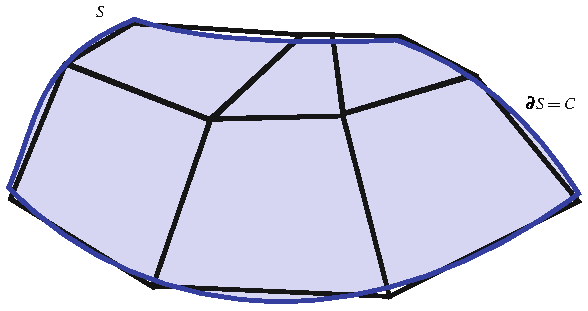
\includegraphics[width=0.696\linewidth]{images/vector/fig-9-16.pdf}
  \caption{边界为闭曲线 $\partial S=C$ 的曲面 $S$ 被较小的曲面 $S_i$ 覆盖. 当 $\Delta S_i\to0$ 时，曲面 $S$ 被逼近得越来越好}
  \label{fig:9-16}
\end{figure}

通过与上一节类似的推理，如果两个 $C_i$ 共享一条边，我们有
\[
\int_A F\cdot\hat{t}\,ds=-\int_B F\cdot\hat{t}\,ds
\]
所以这些项抵消，见图~\ref{fig:9-17}. 因此
\begin{align*}
\oint_{\partial S=C}F\cdot\hat{t}\,ds=\lim_{\substack{N\to\infty\\|\Delta S_i|\to0}}\sum_{i=0}^{N}\oint_{C_i}F\cdot\hat{t}\,ds
=\lim_{\substack{N\to\infty\\|\Delta S_i|\to0}}\sum_{i=0}^{N}\frac{1}{\Delta S_i}\oint_{C_i}F\cdot\hat{t}\,ds\ \Delta S_i \\
=\lim_{\substack{N\to\infty\\|\Delta S_i|\to0}}\sum_{i=0}^{N}\Bigl(\lim_{|\Delta S_i|\to0}\frac{1}{\Delta S_i}\oint_{C_i}F\cdot\hat{t}\,ds\Bigr)\Delta S_i
=\lim_{\substack{N\to\infty\\|\Delta S_i|\to0}}\sum_{i=0}^{N}\bigl(\hat{n}_i\cdot\operatorname{curl}F\bigr)_i\Delta S_i \\
=\iint_S\bigl(\hat{n}\cdot\operatorname{curl}F\bigr)\,dS,
\end{align*}

\begin{figure}[htbp]
  \centering
  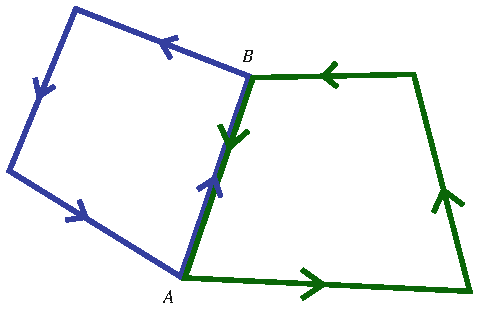
\includegraphics[width=0.568\linewidth]{images/vector/fig-9-17.pdf}
  \caption{共享边界 $C_i$（即点 $A$ 与 $B$ 之间的线段）的两个相邻的子曲面}
  \label{fig:9-17}
\end{figure}

这正是 Stokes 定理：
\begin{theorem}[Stokes 定理]\label{thm:9-4}
\[
\oint_{\partial S}F\cdot\hat{t}\,ds=\iint_S\bigl(\hat{n}\cdot\operatorname{curl}F\bigr)\,dS.
\]
\end{theorem}

写 Stokes 定理的另一种方式是
\[
\oint_{\partial S}F\cdot ds=\iint_S\operatorname{curl}F\cdot dS.
\]

在本节中，我们使用了 $\mathbb{R}^3$ 上用笛卡尔坐标书写的向量场 $F$ 的旋度定义，求出了 $\operatorname{curl}F$ 的表达式. 但当然，第 6.5 节中引入的柱坐标系和球坐标系也是 $\mathbb{R}^3$ 上非常常用的坐标系.

\begin{question}\label{q:9-7}
假设 $F=F_r\hat{e}_r+F_\theta\hat{e}_\theta+F_z\hat{e}_z$ 是关于柱坐标书写的 $\mathbb{R}^3$ 上的向量场. 向量 $\hat{e}_r$ 是 $r$ 增大方向的单位向量，$\hat{e}_\theta$ 是 $\theta$ 增大方向的单位向量，$\hat{e}_z$ 是 $z$ 增大方向的单位向量. 利用与图~\ref{fig:6-14} 中所示柱坐标体积元素的每个面对应的边类似的曲线，以及和本节类似的过程，证明
\[
\operatorname{curl}F=(\operatorname{curl}F)_r\hat{e}_r+(\operatorname{curl}F)_\theta\hat{e}_\theta+(\operatorname{curl}F)_z\hat{e}_z,
\]
其中
\[
(\operatorname{curl}F)_r=\frac{1}{r}\frac{\partial F_z}{\partial\theta}-\frac{\partial F_\theta}{\partial z},\qquad
(\operatorname{curl}F)_\theta=\frac{\partial F_r}{\partial z}-\frac{\partial F_z}{\partial r},\qquad
(\operatorname{curl}F)_z=\frac{1}{r}\frac{\partial(rF_\theta)}{\partial r}-\frac{1}{r}\frac{\partial F_r}{\partial\theta}.
\]
\end{question}

\begin{question}\label{q:9-8}
假设 $F=F_r\hat{e}_r+F_\theta\hat{e}_\theta+F_\varphi\hat{e}_\varphi$ 是关于球坐标书写的 $\mathbb{R}^3$ 上的向量场. 向量 $\hat{e}_r$ 是 $r$ 增大方向的单位向量，$\hat{e}_\theta$ 是 $\theta$ 增大方向的单位向量，$\hat{e}_\varphi$ 是 $\varphi$ 增大方向的单位向量. 利用与图~\ref{fig:6-16} 中所示球坐标体积元素的每个面对应的边类似的曲线，以及和本节类似的过程，证明
\[
\operatorname{curl}F=(\operatorname{curl}F)_r\hat{e}_r+(\operatorname{curl}F)_\theta\hat{e}_\theta+(\operatorname{curl}F)_\varphi\hat{e}_\varphi,
\]
其中
\begin{align*}
(\operatorname{curl}F)_r=\frac{1}{r\sin\theta}\frac{\partial(\sin\theta\,F_\varphi)}{\partial\theta}-\frac{1}{r\sin\theta}\frac{\partial F_\theta}{\partial\varphi},\qquad
(\operatorname{curl}F)_\theta=\frac{1}{r\sin\theta}\frac{\partial F_r}{\partial\varphi}-\frac{1}{r}\frac{\partial(rF_\varphi)}{\partial r}, \\
(\operatorname{curl}F)_\varphi=\frac{1}{r}\frac{\partial(rF_\theta)}{\partial r}-\frac{1}{r}\frac{\partial F_r}{\partial\theta}.
\end{align*}
\end{question}

\section{梯度}

梯度比散度或旋度更直截了当. 在向量微积分中，函数 $f:\mathbb{R}^3\to\mathbb{R}$ 的梯度通常简单地定义为向量场
\[
\operatorname{grad}f=\frac{\partial f}{\partial x}\hat{\imath}+\frac{\partial f}{\partial y}\hat{\jmath}+\frac{\partial f}{\partial z}\hat{k}.
\]
一般 $\operatorname{grad}f$ 写成 $\nabla f$. 此外，在向量微积分中我们还学到，函数 $f$ 沿单位长度向量 $u$ 方向的方向导数可以写成 $D_uf=\nabla f\cdot u$，或者写成 $u[f]=\nabla f\cdot u$.

我们基本上是反过来定义函数 $f$ 的梯度：把它定义为与单位长度向量 $u$ 点积后给出 $f$ 沿方向 $u$ 的方向导数的那个向量场：
\begin{definition}[梯度的定义]\label{def:9-3-1}
\[
\operatorname{grad}f\cdot u=u[f].
\]
\end{definition}

在第 2.3 节中我们基本上证明了，在使用笛卡尔坐标系时可以写成
\begin{theorem}[梯度的计算公式（笛卡尔坐标）]\label{thm:9-5}
\[
\operatorname{grad}f=\frac{\partial f}{\partial x}\hat{\imath}+\frac{\partial f}{\partial y}\hat{\jmath}+\frac{\partial f}{\partial z}\hat{k}.
\]
\end{theorem}
因此我们看到，通常的向量微积分定义与我们的定义一致. 当然，在这一点上你应该看到 $f$ 的梯度 $\operatorname{grad}f$ 与 1-形式 $df$ 之间的相似之处.

我们在上一节已经讨论了向量场沿曲线的积分是什么. 向量场 $F$ 沿曲线 $C$ 的积分由 $\int_C F\cdot\hat{t}\,ds$ 给出，其中 $\hat{t}$ 是沿曲线 $C$ 的单位切向量，曲线由弧长 $s$ 参数化. 把曲线写成 $C=c(s)=\bigl(x(s),y(s),z(s)\bigr)$，那么我们有
\[
c'(s)=\Bigl(\frac{dx}{ds},\frac{dy}{ds},\frac{dz}{ds}\Bigr)=\frac{dx}{ds}\hat{\imath}+\frac{dy}{ds}\hat{\jmath}+\frac{dz}{ds}\hat{k},
\]
这显然是曲线 $c(s)$ 的切线. 另外，与上面类似的方式，我们可以形式上写 $c'(s)\,ds=\hat{\imath}dx+\hat{\jmath}dy+\hat{k}dz$ 并把它定义为 $ds$. 假设我们令 $F=\operatorname{grad}f$，那么 $\operatorname{grad}f$ 沿曲线 $c(s)$ 从 $c(a)$ 到 $c(b)$（其中 $a,b\in\mathbb{R}$ 且 $a\leq b$）的积分将是
\[
\begin{aligned}
\int_C\operatorname{grad}f\cdot c'(s)\,ds
&=\int_a^b\Bigl(\frac{\partial f}{\partial x}\hat{\imath}+\frac{\partial f}{\partial y}\hat{\jmath}+\frac{\partial f}{\partial z}\hat{k}\Bigr)\cdot\Bigl(\frac{dx}{ds}\hat{\imath}+\frac{dy}{ds}\hat{\jmath}+\frac{dz}{ds}\hat{k}\Bigr)\,ds\\
&=\int_a^b\Bigl(\frac{\partial f}{\partial x}\frac{dx}{ds}+\frac{\partial f}{\partial y}\frac{dy}{ds}+\frac{\partial f}{\partial z}\frac{dz}{ds}\Bigr)\,ds\\
&=\int_a^b\frac{d}{ds}f\bigl(c(s)\bigr)\,ds\\
&=f\bigl(c(b)\bigr)-f\bigl(c(a)\bigr).
\end{aligned}
\]
倒数第二个等式来自链式法则，最后一个等式来自微积分基本定理. 把 $c'(s)\,ds$ 写成 $ds$，就得到线积分基本定理：
\begin{theorem}[线积分基本定理]\label{thm:9-6}
\[
\int_C\operatorname{grad}f\cdot ds=f\bigl(c(b)\bigr)-f\bigl(c(a)\bigr).
\]
\end{theorem}

在柱坐标中，类似的论证会给出
\[
\operatorname{grad}f=\frac{\partial f}{\partial r}\hat{e}_r+\frac{1}{r}\frac{\partial f}{\partial\theta}\hat{e}_\theta+\frac{\partial f}{\partial z}\hat{e}_z,
\]
其中 $\hat{e}_r$ 是 $r$ 增大方向的单位向量，$\hat{e}_\theta$ 是 $\theta$ 增大方向的单位向量，$\hat{e}_z$ 是 $z$ 增大方向的单位向量. 在球坐标中我们有
\[
\operatorname{grad}f=\frac{\partial f}{\partial r}\hat{e}_r+\frac{1}{r}\frac{\partial f}{\partial\theta}\hat{e}_\theta+\frac{1}{r\sin\theta}\frac{\partial f}{\partial\varphi}\hat{e}_\varphi,
\]
其中当然 $\hat{e}_r$ 是 $r$ 增大方向的单位向量，$\hat{e}_\theta$ 是 $\theta$ 增大方向的单位向量，$\hat{e}_\varphi$ 是 $\varphi$ 增大方向的单位向量.

\begin{question}\label{q:9-9}
函数 $f$ 的\newterm{laplacian}{拉普拉斯算子}{Laplacian}定义为 $\operatorname{div}(\operatorname{grad}f)=\nabla\cdot(\nabla f)=\nabla\cdot\nabla f$. 有时这写成 $\nabla^2f$ 或 $\Delta f$. 求 $f$ 在笛卡尔坐标、柱坐标和球坐标下的拉普拉斯算子.
\end{question}

\section{上下指标、升号与降号}

在继续之前，现在是引入一种特定记号约定的好时机. 这种记号约定对后续内容将很有用. 到目前为止，在这本书中我们一直在努力解释数学概念，因此主要使用数学记号. 然而，随着我们走向许多其他例子和主题，物理学中通常使用的记号将很有用.

不同的记号各有其优缺点，而微分几何就是数学中记号负担很重的领域之一. 数学记号擅长理解理论、理解数学对象实际上是什么、理解数学对象所在的空间，以及理解底层的数学运算和作用. 物理学记号通常更适合进行计算和演算，尽管这种记号可能会掩盖计算底下的数学实质. 要成为一个好的数学家或物理学家，你真的需要对这两种记号都感到自如.

首先我们引入 \newterm{einstein-summation}{Einstein 求和记号}{Einstein summation notation}. 简而言之，Einstein 求和记号的要点是：当你看到重复出现的上下指标时就要求和. 也就是说，如果你看到像
\[
a^ie_i
\]
这样的东西，它实际上表示
\[
\sum_i a^ie_i.
\]
类似地，
\[
a_ie^i\equiv\sum_i a_ie^i.
\]
据说 Einstein 曾经打趣说，求和记号是他对数学的伟大贡献！求和记号在张量微积分中被广泛使用，我们将在附录 A 中引入张量微积分. 暂不讨论这个表达式的含义，考虑
\[
T^{ijk}_{lm}\Lambda^{l}_{jk}.
\]
用 Einstein 求和记号，这实际上表示
\[
\sum_j\sum_k\sum_l T^{ijk}_{lm}\Lambda^{l}_{jk}.
\]
正如你所看到的，每当下指标和上指标重复出现时，我们就对该指标求和. 由于同时存在成对出现的上指标和下指标 $j$、$k$ 和 $l$，我们对 $j$、$k$ 和 $l$ 求和.

考虑向量空间 $V=\operatorname{span}\{e_1,e_2,e_3\}$. $V$ 的元素可以借助系数用基向量 $e_1,e_2,e_3$ 写出. 也就是说，$v\in V$ 可以写成
\[
v=v^1e_1+v^2e_2+v^3e_3=\begin{bmatrix}v^1\\v^2\\v^3\end{bmatrix}=v^ie_i,
\]
其中向量系数 $v^1,v^2,v^3$ 是实数. 注意向量系数用上指标书写. 和往常一样，我们继续把向量看成列矩阵.

$V$ 的对偶空间是 $V^*=\operatorname{Span}\{e^{1*},e^{2*},e^{3*}\}$，其中 $e^{1*},e^{2*},e^{3*}$ 只是 $e_1,e_2,e_3$ 的对偶元素. 也就是说，我们有
\[
\langle e^{i*},e_j\rangle=\delta_{ij}=\begin{cases}1,&i=j,\\0,&i\neq j.\end{cases}
\]
为了从现在起与 Einstein 求和记号保持一致，我们将用上指标书写对偶基元素 $e^1,e^2,e^3$. 也就是说，$e^{1*}\equiv e^1$、$e^{2*}\equiv e^2$、$e^{3*}\equiv e^3$，所以 $\langle e^i,e_j\rangle=e^i(e_j)=\delta^i_j$. 有时你会看到克罗内克 δ 函数写成 $\delta^i_j$，以与 Einstein 求和记号保持一致. $V^*=\operatorname{Span}\{e^1,e^2,e^3\}$ 的元素（有时称为余向量）写成
\[
\alpha=\alpha_1e^1+\alpha_2e^2+\alpha_3e^3=[\alpha_1,\alpha_2,\alpha_3]=\alpha_ie^i,
\]
其中余向量系数 $\alpha_1,\alpha_2,\alpha_3$ 是实数. 再次注意，余向量系数用下指标书写. 和往常一样，我们继续把余向量看成行矩阵. 所以
\[
\begin{aligned}
\langle\alpha,v\rangle=\alpha(v)&=(\alpha_1e^1+\alpha_2e^2+\alpha_3e^3)(v^1e_1+v^2e_2+v^3e_3)\\
&=\alpha_1e^1(v^1e_1+v^2e_2+v^3e_3)+\alpha_2e^2(v^1e_1+v^2e_2+v^3e_3)\\
&\quad+\alpha_3e^3(v^1e_1+v^2e_2+v^3e_3)\\
&=\alpha_1v^1e^1(e_1)+\alpha_1v^2e^1(e_2)+\alpha_1v^3e^1(e_3)\\
&\quad+\alpha_2v^1e^2(e_1)+\alpha_2v^2e^2(e_2)+\alpha_2v^3e^2(e_3)\\
&\quad+\alpha_3v^1e^3(e_1)+\alpha_3v^2e^3(e_2)+\alpha_3v^3e^3(e_3)\\
&=\alpha_1v^1+\alpha_2v^2+\alpha_3v^3.
\end{aligned}
\]
多么凌乱的计算，如果你有比三个多很多的基元素，你不会想这样做，尽管模式当然很清楚. 用传统求和记号做同样的计算是
\[
\begin{aligned}
\langle\alpha,v\rangle=\alpha(v)&=\Bigl(\sum_{i=1}^{3}\alpha_ie^i\Bigr)\Bigl(\sum_{j=1}^{3}v^je_j\Bigr)=\sum_{i=1}^{3}\alpha_ie^i\Bigl(\sum_{j=1}^{3}v^je_j\Bigr)\\
&=\sum_{i=1}^{3}\sum_{j=1}^{3}\alpha_iv^je^i(e_j)=\sum_{i=1}^{3}\alpha_iv^i.\qquad(\text{只有 }j=i\text{ 的项保留下来})
\end{aligned}
\]
最后我们用 Einstein 求和记号做同样的计算：
\[
\begin{aligned}
\langle\alpha,v\rangle=\alpha(v)&=(\alpha_ie^i)(v^je_j)=\alpha_ie^i(v^je_j)\\
&=\alpha_iv^je^i(e_j)=\alpha_iv^i.\qquad(\text{只有 }j=i\text{ 的项保留下来})
\end{aligned}
\]
一旦你对 Einstein 求和记号感到自如，你的手就不用动那么多了.

现在，让我们在微分形式的语境下看看这一切. 目前我们假设 $M=\mathbb{R}^3$. 我们将 $M$ 的笛卡尔坐标函数写成 $x^1,x^2,x^3$，用上指标而不是下指标. 数学家倾向于对坐标函数使用下指标，事实上到目前为止我们正是这样做的，但通过用上指标书写坐标函数，Einstein 求和记号就能漂亮地工作. 所以，在点 $p\in M$ 处，切空间由
\[
T_p\mathbb{R}^3=\operatorname{span}\Bigl\{\left.\frac{\partial}{\partial x^1}\right|_p,\left.\frac{\partial}{\partial x^2}\right|_p,\left.\frac{\partial}{\partial x^3}\right|_p\Bigr\}
=\operatorname{span}\Bigl\{\frac{\partial}{\partial x^1},\frac{\partial}{\partial x^2},\frac{\partial}{\partial x^3}\Bigr\}
\]
给出，其中第二行在记号中省略了基点. 点 $p\in M$ 处的余切空间由
\[
T_p^*\mathbb{R}^3=\operatorname{Span}\Bigl\{\left.dx^1\right|_p,\left.dx^2\right|_p,\left.dx^3\right|_p\Bigr\}
=\operatorname{Span}\{dx^1,dx^2,dx^3\}
\]
给出. 显然我们可以把 $dx^i$ 中的指标看成上指标. 按照惯例，我们把 $\frac{\partial}{\partial x^i}$ 中的指标看成下指标，因为它位于表达式的``分母''中. 因此 $v\in T_p\mathbb{R}^3$ 的元素写成
\[
v=v^1\frac{\partial}{\partial x^1}+v^2\frac{\partial}{\partial x^2}+v^3\frac{\partial}{\partial x^3}=v^i\frac{\partial}{\partial x^i},
\]
其中 $v^1,v^2,v^3$ 是实数. 再次地，向量的系数用上指标书写. $\alpha\in T_p^*\mathbb{R}^3$ 的元素写成
\[
\alpha=\alpha_1dx^1+\alpha_2dx^2+\alpha_3dx^3=\alpha_idx^i,
\]
其中 $\alpha_1,\alpha_2,\alpha_3$ 是实数. 正如我们看到的，余向量，即微分形式，其系数用下指标书写.

总之，向量基元素用下指标书写，向量分量用上指标书写. 余向量（微分形式）基元素用上指标书写，余向量（微分形式）分量用下指标书写.

现在我们引入所谓的\newterm{musical-isomorphism}{音乐同构}{musical isomorphism}. 实际上，音乐同构依赖于一种称为\newterm{metric}{度规}{metric}的东西. 非常粗略地，你可以把度规想成允许你测量两点之间距离的东西. 我们将在引入张量之后讨论欧几里得度规，但本质上它就是我们熟悉的 $\mathbb{R}^n$ 上通常的距离函数. 然而，现在我们还不会那么数学严格，而是给出一个不显式依赖度规的音乐同构的``定义''. 你只要记住，目前我们算是把一些数学理论扫到地毯下面了.

音乐同构之所以称为``音乐''的，是因为所用的记号——\newterm{flat}{降号}{flat} $\flat$ 和\newterm{sharp}{升号}{sharp} $\sharp$. 如果你唱过歌或演奏过乐器，你就知道 $\flat$ 告诉你把音符的音高降低，而 $\sharp$ 告诉你把音符的音高升高. 类似地，$\flat$ 同构被称为``降低指标''，而 $\sharp$ 同构被称为``升高指标''.

$\flat$ 同构由
\[
\flat:T_pM\longrightarrow T_p^*M,\qquad v^i\frac{\partial}{\partial x^i}\longmapsto v_idx^i,\quad\text{其中 }v_i=v^i
\]
给出. 这种映射的写法是 $v^{\flat}$，就像乐谱中降号的写法一样，所以我们写
\[
v^{\flat}=\Bigl(v^i\frac{\partial}{\partial x^i}\Bigr)^{\flat}\equiv v_idx^i,
\]
其中 $v_i=v^i$. 例如我们有
\[
\Bigl(7\frac{\partial}{\partial x^1}+3\frac{\partial}{\partial x^2}-6\frac{\partial}{\partial x^3}\Bigr)^{\flat}=7dx^1+3dx^2-6dx^3.
\]
注意正在发生的事情：我们把一个向量（其分量用上指标书写）变成一个 1-形式（其分量用下指标书写），所以我们是在``降低''指标，这就解释了使用 $\flat$ 符号的原因.

$\sharp$ 同构由
\[
\sharp:T_p^*M\longrightarrow T_pM,\qquad \alpha_idx^i\longmapsto\alpha^i\frac{\partial}{\partial x^i},\quad\text{其中 }\alpha^i=\alpha_i
\]
给出. 同样，这种映射的写法是 $\alpha^{\sharp}$，就像乐谱中升号的写法一样，所以我们写
\[
\alpha^{\sharp}=\Bigl(\alpha_idx^i\Bigr)^{\sharp}\equiv\alpha^i\frac{\partial}{\partial x^i},
\]
其中 $\alpha^i=\alpha_i$. 例如我们有
\[
\bigl(3dx^1-9dx^2+8dx^3\bigr)^{\sharp}=3\frac{\partial}{\partial x^1}-9\frac{\partial}{\partial x^2}+8\frac{\partial}{\partial x^3}.
\]
我们正在把一个微分 1-形式（或余向量）（其分量用下指标书写）变成一个向量（其分量用上指标书写），所以我们是在``升高''指标，这就解释了使用 $\sharp$ 符号的原因.

你应该注意，降号和升号算子的这些``定义''只有在用笛卡尔坐标书写我们的向量和 1-形式时才有效. 这是我们没有用流形上的度规给出降号和升号算子的真正定义所付出的代价. 所以目前，我们只能对用笛卡尔坐标书写的向量取降号、对用笛卡尔坐标书写的 1-形式取升号，但如果我们的向量或 1-形式是相对于任何其他坐标系书写的，则不能这样做.

如果 $F$ 是 $M$ 上的向量场，即切丛 $TM$ 的一个截面，那么 $F^{\flat}$ 是 $M$ 上的微分 1-形式，即余切丛 $T^*M$ 的一个截面. 如果 $\alpha$ 是 $M$ 上的微分 1-形式，即余切丛 $T^*M$ 的一个截面，那么 $\alpha^{\sharp}$ 是 $M$ 上的向量场，即切丛 $TM$ 的一个截面. 回想我们总是把向量写成列矩阵、把 1-形式写成行矩阵，我们可以把 $\flat$ 想成把列矩阵变成行矩阵，把 $\sharp$ 想成把行矩阵变成列矩阵.

现在，让我们非常简短地回忆第 5.6 节的 Hodge 星算子. 我们曾经计算过下面的 Hodge 星映射
\begin{align*}
\ast:\Lambda^0(\mathbb{R}^3)\longrightarrow\Lambda^3(\mathbb{R}^3),\qquad
\ast:\Lambda^1(\mathbb{R}^3)\longrightarrow\Lambda^2(\mathbb{R}^3), \\
\ast:\Lambda^2(\mathbb{R}^3)\longrightarrow\Lambda^1(\mathbb{R}^3),\qquad
\ast:\Lambda^3(\mathbb{R}^3)\longrightarrow\Lambda^0(\mathbb{R}^3),
\end{align*}
它们由
\begin{align*}
\ast 1=dx^1\wedge dx^2\wedge dx^3=dx\wedge dy\wedge dz, \\
\ast dx=dy\wedge dz,\qquad\ast dy=dz\wedge dx,\qquad\ast dz=dx\wedge dy, \\
\ast(dy\wedge dz)=dx,\qquad\ast(dz\wedge dx)=dy,\qquad\ast(dx\wedge dy)=dz, \\
\ast(dx\wedge dy\wedge dz)=1
\end{align*}
给出.

假设我们有向量场 $F=P\frac{\partial}{\partial x}+Q\frac{\partial}{\partial y}+R\frac{\partial}{\partial z}$. 我们将定义映射 $(\ast\circ\flat)$：先把向量场取降号得到一个 1-形式，再对该 1-形式取 Hodge 星得到一个 2-形式：
\[
(\ast\circ\flat)F\equiv\ast(F^{\flat})=\ast(Pdx+Qdy+Rdz)=Pdy\wedge dz+Qdz\wedge dx+Rdx\wedge dy.
\]
有了这最后一个映射，我们现在准备考察标准向量微积分与微分形式之间的关系.

\section{与微分形式的关系}

\subsection{梯度、旋度、散度与外微分}

理解微分形式与向量微积分之间的关系实际上不过是看到恰当的映射能使一切都优美地成立. 我们将本质上一个一个地考察每个部分. 在这个过程的进行中，我们将发现广义 Stokes 定理，通常简称为 Stokes 定理. 广义 Stokes 定理，通常简称为 Stokes 定理，是你已经知道的三个向量微积分定理的同时推广：
\begin{itemize}
  \item 线积分基本定理，
  \item （向量微积分的）Stokes 定理，
  \item （向量微积分的）散度定理.
\end{itemize}
广义 Stokes 定理将使我们能用微分形式以非常漂亮而紧凑的方式重写这三个定理.

现在我们将证明下面的图表交换.
\[
\begin{array}{ccc}
C(\mathbb{R}^3)&\xrightarrow{\ \operatorname{grad}\ }&T\mathbb{R}^3\\[3pt]
\Big\downarrow \mathrm{id}&&\Big\downarrow \flat\\[3pt]
\Lambda^0(\mathbb{R}^3)&\xrightarrow{\ \ d\ \ }&\Lambda^1(\mathbb{R}^3)
\end{array}
\]
首先我们确保回忆四个角上的空间是什么. 左上角是空间 $C(\mathbb{R}^3)$，它不过是流形 $\mathbb{R}^3$ 上的连续函数空间. 右上角的空间 $T\mathbb{R}^3$ 不过是 $\mathbb{R}^3$ 的切丛，它包含 $\mathbb{R}^3$ 上的所有向量场. 左下角是 $\Lambda^0(\mathbb{R}^3)$，即 $\mathbb{R}^3$ 上的 0-形式，它们就是 $\mathbb{R}^3$ 上的连续函数. 注意空间 $\Lambda^0(\mathbb{R}^3)$ 与 $C(\mathbb{R}^3)$ 是完全相同的空间. 右下角是空间 $\Lambda^1(\mathbb{R}^3)=T^*\mathbb{R}^3$，即 $\mathbb{R}^3$ 上的 1-形式. 这些空间之间的映射是 $\operatorname{grad}$、$\flat$、$d$ 和 $\mathrm{id}$，即恒等映射.

``图表交换''是那些数学短语之一，如果你主修数学你会经常听到，即使你是物理专业的学生，你也会不时听到它. 让我们花一点时间解释它是什么意思. 如果你从一个函数 $f\in C(\mathbb{R}^3)$ 出发，那么无论你走哪条路，是横穿顶部然后从右侧向下，还是从左侧向下然后横穿底部，你都会在 $\Lambda^1(\mathbb{R}^3)$ 中得到同一个元素. 也就是说，我们有
\[
(\operatorname{grad}f)^{\flat}=d\bigl(\mathrm{id}(f)\bigr).
\]
所以说上面的图表交换，与说 $(\operatorname{grad}f)^{\flat}=d\bigl(\mathrm{id}(f)\bigr)=df$ 完全是一回事. 现在我们来证明这个等式. 给定 $\mathbb{R}^3$ 上的函数 $f\in C(\mathbb{R}^3)$，我们知道 $\operatorname{grad}$ 根据
\[
\nabla f=\frac{\partial f}{\partial x}\hat{\imath}+\frac{\partial f}{\partial y}\hat{\jmath}+\frac{\partial f}{\partial z}\hat{k}
=\frac{\partial f}{\partial x}\frac{\partial}{\partial x}+\frac{\partial f}{\partial y}\frac{\partial}{\partial y}+\frac{\partial f}{\partial z}\frac{\partial}{\partial z}
\]
把该函数变成向量场 $\nabla f\in T(\mathbb{R}^3)$. 对这个取降号，我们有
\[
(\nabla f)^{\flat}=\frac{\partial f}{\partial x}dx+\frac{\partial f}{\partial y}dy+\frac{\partial f}{\partial z}dz.
\]
注意，这恰好等于 $f$ 的外微分
\[
df=\frac{\partial f}{\partial x}dx+\frac{\partial f}{\partial y}dy+\frac{\partial f}{\partial z}dz,
\]
因此我们已经证明
\[
df=(\nabla f)^{\flat}.
\]
类似地，我们想证明下面的图表也交换.
\[
\begin{array}{ccc}
T\mathbb{R}^3&\xrightarrow{\ \operatorname{curl}\ }&T\mathbb{R}^3\\[3pt]
\Big\downarrow \flat&&\Big\downarrow {\ast\circ\flat}\\[3pt]
\Lambda^1(\mathbb{R}^3)&\xrightarrow{\ \ d\ \ }&\Lambda^2(\mathbb{R}^3)
\end{array}
\]
也就是说，我们想证明 $d(F^{\flat})=(\ast\circ\flat)(\operatorname{curl}F)$. 给定一个向量场 $F\in T(\mathbb{R}^3)$. 回想我们在上一节定义的映射 $(\ast\circ\flat)F\equiv\ast(F^{\flat})$，我们想求 $(\ast\circ\flat)(\operatorname{curl}F)$. 首先，我们知道
\[
\operatorname{curl}F=\Bigl(\frac{\partial R}{\partial y}-\frac{\partial Q}{\partial z}\Bigr)\frac{\partial}{\partial x}+\Bigl(\frac{\partial P}{\partial z}-\frac{\partial R}{\partial x}\Bigr)\frac{\partial}{\partial y}+\Bigl(\frac{\partial Q}{\partial x}-\frac{\partial P}{\partial y}\Bigr)\frac{\partial}{\partial z}.
\]
所以我们得到
\begin{align*}
(\ast\circ\flat)(\operatorname{curl}F)=\ast\bigl((\operatorname{curl}F)^{\flat}\bigr) \\
=\ast\Bigl[\Bigl(\frac{\partial R}{\partial y}-\frac{\partial Q}{\partial z}\Bigr)dx+\Bigl(\frac{\partial P}{\partial z}-\frac{\partial R}{\partial x}\Bigr)dy+\Bigl(\frac{\partial Q}{\partial x}-\frac{\partial P}{\partial y}\Bigr)dz\Bigr] \\
=\Bigl(\frac{\partial R}{\partial y}-\frac{\partial Q}{\partial z}\Bigr)dy\wedge dz+\Bigl(\frac{\partial P}{\partial z}-\frac{\partial R}{\partial x}\Bigr)dz\wedge dx+\Bigl(\frac{\partial Q}{\partial x}-\frac{\partial P}{\partial y}\Bigr)dx\wedge dy.
\end{align*}
现在我们想计算 $d(F^{\flat})$. 首先我们求
\[
F^{\flat}=\Bigl(P\frac{\partial}{\partial x}+Q\frac{\partial}{\partial y}+R\frac{\partial}{\partial z}\Bigr)^{\flat}=Pdx+Qdy+Rdz.
\]
然后我们取这个的外微分：
\[
\begin{aligned}
d(F^{\flat})&=d(Pdx+Qdy+Rdz)=dP\wedge dx+dQ\wedge dy+dR\wedge dz\\
&=\Bigl(\frac{\partial P}{\partial x}dx+\frac{\partial P}{\partial y}dy+\frac{\partial P}{\partial z}dz\Bigr)\wedge dx+\Bigl(\frac{\partial Q}{\partial x}dx+\frac{\partial Q}{\partial y}dy+\frac{\partial Q}{\partial z}dz\Bigr)\wedge dy\\
&\quad+\Bigl(\frac{\partial R}{\partial x}dx+\frac{\partial R}{\partial y}dy+\frac{\partial R}{\partial z}dz\Bigr)\wedge dz\\
&=\frac{\partial P}{\partial y}dy\wedge dx+\frac{\partial P}{\partial z}dz\wedge dx+\frac{\partial Q}{\partial x}dx\wedge dy+\frac{\partial Q}{\partial z}dz\wedge dy\\
&\quad+\frac{\partial R}{\partial x}dx\wedge dz+\frac{\partial R}{\partial y}dy\wedge dz\\
&=\Bigl(\frac{\partial R}{\partial y}-\frac{\partial Q}{\partial z}\Bigr)dy\wedge dz+\Bigl(\frac{\partial P}{\partial z}-\frac{\partial R}{\partial x}\Bigr)dz\wedge dx+\Bigl(\frac{\partial Q}{\partial x}-\frac{\partial P}{\partial y}\Bigr)dx\wedge dy.
\end{aligned}
\]
因此我们刚刚证明了 $d(F^{\flat})=(\ast\circ\flat)(\operatorname{curl}F)$. 最后，我们想证明这个图表交换.
\[
\begin{array}{ccc}
T\mathbb{R}^3&\xrightarrow{\ \operatorname{div}\ }&C(\mathbb{R}^3)\\[3pt]
\Big\downarrow {\ast\circ\flat}&&\Big\downarrow \ast\\[3pt]
\Lambda^2(\mathbb{R}^3)&\xrightarrow{\ \ d\ \ }&\Lambda^3(\mathbb{R}^3)
\end{array}
\]
给定 $F$，我们有
\[
\operatorname{div}F=\frac{\partial P}{\partial x}+\frac{\partial Q}{\partial y}+\frac{\partial R}{\partial z}.
\]
对这个取 Hodge 星，我们有
\[
\ast(\operatorname{div}F)=\ast\Bigl(\frac{\partial P}{\partial x}+\frac{\partial Q}{\partial y}+\frac{\partial R}{\partial z}\Bigr)=\Bigl(\frac{\partial P}{\partial x}+\frac{\partial Q}{\partial y}+\frac{\partial R}{\partial z}\Bigr)dx\wedge dy\wedge dz.
\]
接下来，我们求
\[
(\ast\circ\flat)F=\ast(F^{\flat})=\ast(Pdx+Qdy+Rdz)=Pdy\wedge dz+Qdz\wedge dx+Rdx\wedge dy,
\]
然后取这个的外微分：
\[
\begin{aligned}
d\bigl((\ast\circ\flat)F\bigr)&=d(Pdy\wedge dz+Qdz\wedge dx+Rdx\wedge dy)\\
&=dP\wedge dy\wedge dz+dQ\wedge dz\wedge dx+dR\wedge dx\wedge dy\\
&=\frac{\partial P}{\partial x}dx\wedge dy\wedge dz+\frac{\partial Q}{\partial y}dy\wedge dz\wedge dx+\frac{\partial R}{\partial z}dz\wedge dx\wedge dy\\
&=\Bigl(\frac{\partial P}{\partial x}+\frac{\partial Q}{\partial y}+\frac{\partial R}{\partial z}\Bigr)dx\wedge dy\wedge dz.
\end{aligned}
\]
因此我们发现
\[
d\bigl((\ast\circ\flat)F\bigr)=\ast(\operatorname{div}F),
\]
这正是我们想找的. 当我们把这三个图表连接在一起时，得到的是：
\[
\begin{array}{ccccccccc}
C(\mathbb{R}^3)&\xrightarrow{\ \operatorname{grad}\ }&T\mathbb{R}^3&\xrightarrow{\ \operatorname{curl}\ }&T\mathbb{R}^3&\xrightarrow{\ \operatorname{div}\ }&C(\mathbb{R}^3)\\[2pt]
\Big\downarrow \mathrm{id}&&\Big\downarrow \flat&&\Big\downarrow {\ast\circ\flat}&&\Big\downarrow \ast\\[2pt]
\Lambda^0(\mathbb{R}^3)&\xrightarrow{\ \ d\ \ }&\Lambda^1(\mathbb{R}^3)&\xrightarrow{\ \ d\ \ }&\Lambda^2(\mathbb{R}^3)&\xrightarrow{\ \ d\ \ }&\Lambda^3(\mathbb{R}^3)
\end{array}
\]
所以，我们非常清楚地看到了三个向量微积分算子与外微分之间的关系. 梯度、旋度和散度不是别的，正是换了外衣的外微分. 向量微积分结果是在 $\mathbb{R}^3$ 上表述和呈现外微分与微分形式的另一种方式. 在向量微积分中，一切都保持为向量，却以与形式相同的方式被利用. 向量微积分的问题是它不能推广到 $n>3$ 的 $\mathbb{R}^n$ 或一般的流形，而我们的微分形式和外微分的概念可以推广到 $n>3$ 的 $\mathbb{R}^n$ 以及一般的流形.

\begin{question}\label{q:9-10}
令 $F=P\hat{\imath}+Q\hat{\jmath}+R\hat{k}$ 是一个向量场，$f$ 是一个连续函数. 证明
\begin{enumerate}
  \item[(a)] 证明 $\operatorname{curl}(\operatorname{grad}f)=0$.
  \item[(b)] 证明 $\operatorname{div}(\operatorname{curl}F)=0$.
  \item[(c)] 解释为什么根据你对外微分 $d$ 的了解，你会预期如此.
\end{enumerate}
\end{question}

\begin{question}\label{q:9-11}
证明下面的恒等式：
\begin{enumerate}
  \item[(a)] $\operatorname{grad}f=(df)^{\sharp}$.
  \item[(b)] $\operatorname{curl}F=\bigl[\ast\bigl(dF^{\flat}\bigr)\bigr]^{\sharp}$.
  \item[(c)] $\operatorname{div}F=\ast\,d\bigl(\ast(F^{\flat})\bigr)$.
  \item[(d)] 对向量场 $v$ 和 $w$，有 $v\times w=\bigl[\ast\bigl(v^{\flat}\wedge w^{\flat}\bigr)\bigr]^{\sharp}$.
  \item[(e)] $(v\cdot w)dx\wedge dy\wedge dz=v^{\flat}\wedge\ast(w^{\flat})$.
\end{enumerate}
\end{question}

\subsection{线积分基本定理}

现在，让我们来看线积分基本定理. 假设我们有一条曲线 $C$，由 $c(s)=\bigl(x(s),y(s),z(s)\bigr)$ 给出，端点为 $c(a)=\bigl(x(a),y(a),z(a)\bigr)$ 和 $c(b)=\bigl(x(b),y(b),z(b)\bigr)$，其中 $a,b\in\mathbb{R}$ 且 $a\leq b$，那么线积分基本定理由
\[
\int_C(\operatorname{grad}f)\cdot ds=f\bigl(c(b)\bigr)-f\bigl(c(a)\bigr)
\]
给出. 我们将把曲线 $C$ 的边界写成 $\partial C=\bigl\{c(b)\bigr\}-\bigl\{c(a)\bigr\}$. 边界将在第 11 章中深入解释. 通过这样做，我们可以把 $f\bigl(c(b)\bigr)-f\bigl(c(a)\bigr)$ 看成或定义为 $f$ 在 $\partial C$ 上的积分的退化形式，即
\[
\int_{\partial C}f\equiv f\bigl(c(b)\bigr)-f\bigl(c(a)\bigr).
\]
我们承认，这个零维情形的记号可能看起来有点做作，但通过这个定义，我们能够为广义 Stokes 定理拥有一个一致的记号. 这使我们能把线积分基本定理的右边写成 $\int_{\partial C}f$.

让曲线 $C$ 由 $s$ 参数化并由 $c$ 给出，所以 $C=c(s)=\bigl(x(s),y(s),z(s)\bigr)$，且 $c'(s)=\frac{dx}{ds}\hat{\imath}+\frac{dy}{ds}\hat{\jmath}+\frac{dz}{ds}\hat{k}$. 如果 $F$ 是一个向量场，我们有 $F$ 沿 $C$ 的积分为
\[
\begin{aligned}
\int_C F\cdot ds&\equiv\int_C F\cdot c'(s)\,ds\\
&=\int_C\Bigl(P\hat{\imath}+Q\hat{\jmath}+R\hat{k}\Bigr)\cdot\Bigl(\frac{dx}{ds}\hat{\imath}+\frac{dy}{ds}\hat{\jmath}+\frac{dz}{ds}\hat{k}\Bigr)\,ds\\
&=\int_C\Bigl(P\frac{dx}{ds}+Q\frac{dy}{ds}+R\frac{dz}{ds}\Bigr)\,ds\\
&=\int_C F^{\flat}.
\end{aligned}
\]
如果 $F=\operatorname{grad}f$，那么我们就有 $(\operatorname{grad}f)^{\flat}=df$. 换句话说，我们可以把线积分基本定理的右边写成 $\int_C df$. 把这与我们上面得到的结合起来，我们可以把线积分基本定理写成
\[
\int_C df=\int_{\partial C}f.
\]
认识到 $f$ 实际上是一个 0-形式，我们可以把它记为 $\alpha$，而 $C$ 是一个一维流形 $M$，我们可以把线积分基本定理写成
\[
\int_M d\alpha=\int_{\partial M}\alpha.
\]

\subsection{向量微积分中的 Stokes 定理}\label{sec:9-5-3}

现在我们来看向量微积分版本的 Stokes 定理，
\[
\iint_S\operatorname{curl}F\cdot\hat{n}\,dS=\oint_{\partial S}F\cdot c'(s)\,ds.
\]
从上面我们知道可以把 Stokes 定理的右边重写为 $\oint_{\partial S}F^{\flat}$.

对于 Stokes 定理的左边，我们想做与上面类似的事情，这需要我们证明
\[
\iint_S\operatorname{curl}F\cdot\hat{n}\,dS=\iint_S\ast(\operatorname{curl}F)^{\flat}.
\]
为了简化记号，我们实际上将证明
\[
\iint_S F\cdot\hat{n}\,dS=\iint_S\ast F^{\flat}.
\]
然后，我们只需把向量场 $F$ 替换为向量场 $\operatorname{curl}F$ 就能得到所需的恒等式.

然而，与线积分情形中我们证明 $\int_C F\cdot dr=\int_C F^{\flat}$ 时那种整齐的计算不同，这里最容易的办法是回到曲面上通量的基本定义. 这个论证不会很严格，但应该足以帮助你理解正在发生的事情. 具有法向量 $\hat{n}=n_1\hat{\imath}+n_2\hat{\jmath}+n_3\hat{k}$ 的无穷小面积 $dS$ 可以分解成 $xy$ 平面、$yz$ 平面和 $xz$ 平面中的无穷小部分. 这里 $n_1dS$ 是 $dS$ 位于 $yz$ 平面中的那部分. $dS$ 的这一部分具有体积形式 $dy\wedge dz$. 类似地，$n_2dS$ 是 $dS$ 位于 $xz$ 平面中的那部分，具有体积形式 $dz\wedge dx$. 最后，$n_3dS$ 是 $dS$ 位于 $xy$ 平面中的那部分，具有体积形式 $dx\wedge dy$. 见图~\ref{fig:9-18}.

\begin{figure}[htbp]
  \centering
  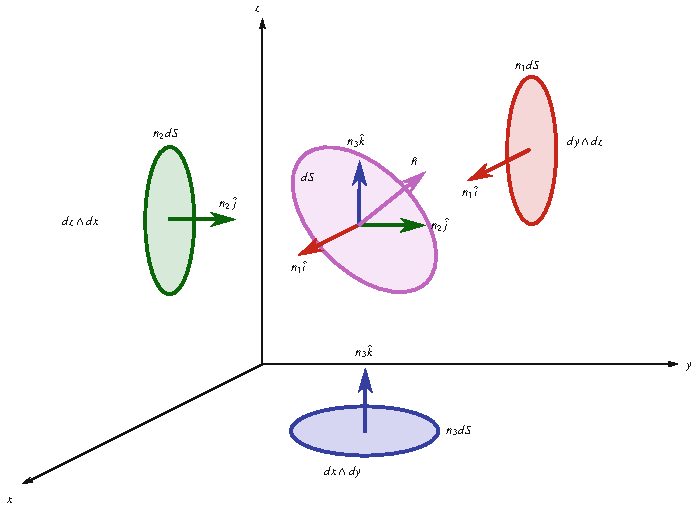
\includegraphics[width=0.960\linewidth]{images/vector/fig-9-18.pdf}
  \caption{带单位法向量 $\hat{n}=n_1\hat{\imath}+n_2\hat{\jmath}+n_3\hat{k}$ 的无穷小面积 $dS$ 被分解为 $n_1dS$、$n_2dS$ 和 $n_3dS$，其单位法向量分别为 $n_1\hat{\imath}$、$n_2\hat{\jmath}$ 和 $n_3\hat{k}$}
  \label{fig:9-18}
\end{figure}

因此我们可以把 $F\cdot\hat{n}\,dS$ 写成 $F\cdot dS$，于是有
\[
\begin{aligned}
\iint_S F\cdot dS&=\iint_S\bigl(P\hat{\imath}+Q\hat{\jmath}+R\hat{k}\bigr)\cdot\bigl(n_1\hat{\imath}+n_2\hat{\jmath}+n_3\hat{k}\bigr)\,dS\\
&=\iint_S(Pn_1+Qn_2+Rn_3)\,dS\\
&=\iint_S\bigl(P\,n_1dS+Q\,n_2dS+R\,n_3dS\bigr)\\
&=\iint_S\bigl(P\,dy\wedge dz+Q\,dz\wedge dx+R\,dx\wedge dy\bigr)\\
&=\iint_S\ast F^{\flat},
\end{aligned}
\]
这正是我们想要证明的. 当我们把 $F$ 替换为 $\operatorname{curl}F$ 时，我们有
\[
\iint_S\operatorname{curl}F\cdot dS=\iint_S\ast(\operatorname{curl}F)^{\flat}=\iint_S d(F^{\flat}).
\]
这样我们就重写了 Stokes 定理的左边. 把右边和左边的部分放在一起，我们可以把向量微积分版本的 Stokes 定理重写为
\[
\iint_S d(F^{\flat})=\oint_{\partial S}F^{\flat}.
\]
显然，$F^{\flat}$ 是一个 1-形式 $\alpha$，而 $S$ 是一个二维流形 $M$，这意味着我们已经把 Stokes 定理写成
\[
\int_M d\alpha=\int_{\partial M}\alpha.
\]

\subsection{散度定理}

最后，我们来看向量微积分中的散度定理，
\[
\iiint_V\operatorname{div}F\,dV=\oint_{\partial V}F\cdot dS.
\]
我们注意到左边的被积函数不是别的，正是 $\ast(\operatorname{div}F)$，它可以重写为 $d\bigl((\ast\circ\flat)F\bigr)$. 我们还看到右边 $\oint_{\partial V}F\cdot dS$ 可以写成 $\oint_{\partial V}\ast(F^{\flat})$. 这使得我们可以把散度定理写成
\[
\iiint_V d\bigl((\ast\circ\flat)F\bigr)=\oint_{\partial V}\ast(F^{\flat}).
\]
把三维流形 $V$ 写成 $M$，把三维 2-形式 $(\ast\circ\flat)F$ 写成 $\alpha$，散度定理就是
\[
\int_M d\alpha=\int_{\partial M}\alpha.
\]
这样我们就用微分形式记号把我们的三个向量微积分定理写成了相同的形式. 这个恒等式
\[
\int_M d\alpha=\int_{\partial M}\alpha
\]
正是我们将在几章之后证明的广义 Stokes 定理.

\section{小结、参考文献与问题}

\subsection{小结}

从几何上讲，散度度量向量场在点 $(x_0,y_0,z_0)$ 处``发散''或``散开''的程度. 给定围绕点 $(x_0,y_0,z_0)$ 的、带边界 $\partial V$ 和体积 $\Delta V$ 的小三维区域 $V$，$F$ 在 $(x_0,y_0,z_0)$ 处的散度定义为
\[
\operatorname{div}F=\lim_{\Delta V\to0}\frac{1}{\Delta V}\oint_{\partial V}F\cdot\hat{n}\,dS.
\]

本质上，旋度度量向量场 $F$ 绕某点无穷小路径的每单位面积的``环流''. 假设 $S$ 是以闭曲线 $C=\partial S$ 为边界的曲面，$\Delta S$ 是该曲面的面积，$\hat{n}$ 是该曲面的单位法向量，$ds$ 中的 $s$ 是无穷小弧长元素，曲面面积 $\Delta S$ 围绕点 $(x_0,y_0,z_0)$ 收缩到零. 那么 $F$ 在点 $(x_0,y_0,z_0)$ 处的旋度定义为
\[
\hat{n}\cdot\operatorname{curl}F=\lim_{|\Delta S|\to0}\frac{1}{\Delta S}\oint_C F\cdot\hat{t}\,ds.
\]

我们基本上是反过来定义函数 $f$ 的梯度：把它定义为与单位长度向量 $u$ 点积后给出 $f$ 沿方向 $u$ 的方向导数的那个向量场，
\[
\operatorname{grad}f\cdot u=u[f].
\]

利用散度、旋度和梯度的这些几何定义，有可能得到向量微积分中的标准公式定义. 令 $F=P\hat{\imath}+Q\hat{\jmath}+R\hat{k}$，我们有
\begin{align*}
\operatorname{div}F=\frac{\partial P}{\partial x}+\frac{\partial Q}{\partial y}+\frac{\partial R}{\partial z}, \\
\operatorname{curl}F=\Bigl(\frac{\partial R}{\partial y}-\frac{\partial Q}{\partial z}\Bigr)\hat{\imath}+\Bigl(\frac{\partial P}{\partial z}-\frac{\partial R}{\partial x}\Bigr)\hat{\jmath}+\Bigl(\frac{\partial Q}{\partial x}-\frac{\partial P}{\partial y}\Bigr)\hat{k}, \\
\operatorname{grad}f=\frac{\partial f}{\partial x}\hat{\imath}+\frac{\partial f}{\partial y}\hat{\jmath}+\frac{\partial f}{\partial z}\hat{k}.
\end{align*}

为了与 Einstein 求和记号保持一致，向量基元素用下指标书写，向量分量用上指标书写. 余向量（微分形式）基元素用上指标书写，余向量（微分形式）分量用下指标书写. 这使我们能够用笛卡尔坐标给出音乐同构. $\flat$ 同构由
\[
\flat:T_pM\longrightarrow T_p^*M,\qquad v^i\frac{\partial}{\partial x^i}\longmapsto v_idx^i,\quad\text{其中 }v_i=v^i
\]
给出，而 $\sharp$ 同构由
\[
\sharp:T_p^*M\longrightarrow T_pM,\qquad \alpha_idx^i\longmapsto\alpha^i\frac{\partial}{\partial x^i},\quad\text{其中 }\alpha^i=\alpha_i
\]
给出. 记住，这些实际上不是音乐同构的数学定义，而只是它们在笛卡尔坐标下的公式. 但连同 Hodge 星算子，这些同构提供了向量微积分与微分形式之间的联系. 下面的图表交换.
\[
\begin{array}{ccccccccc}
C(\mathbb{R}^3)&\xrightarrow{\ \operatorname{grad}\ }&T\mathbb{R}^3&\xrightarrow{\ \operatorname{curl}\ }&T\mathbb{R}^3&\xrightarrow{\ \operatorname{div}\ }&C(\mathbb{R}^3)\\[2pt]
\Big\downarrow \mathrm{id}&&\Big\downarrow \flat&&\Big\downarrow {\ast\circ\flat}&&\Big\downarrow \ast\\[2pt]
\Lambda^0(\mathbb{R}^3)&\xrightarrow{\ \ d\ \ }&\Lambda^1(\mathbb{R}^3)&\xrightarrow{\ \ d\ \ }&\Lambda^2(\mathbb{R}^3)&\xrightarrow{\ \ d\ \ }&\Lambda^3(\mathbb{R}^3)
\end{array}
\]
这使得向量微积分中的下列恒等式可以用外微分写出：
\[
\nabla\times(\nabla f)=0\quad\longleftrightarrow\quad d(df)=0,\qquad
\nabla\cdot(\nabla\times F)=0\quad\longleftrightarrow\quad d(d\alpha)=0.
\]
注意 $d(df)=0$ 和 $d(d\alpha)=0$ 当然只是 Poincaré 引理的推论. 它也使向量微积分中的三个主要定理可以用微分形式写出. 事实上，这三个定理都是微分形式版本 Stokes 定理的特殊情形：
\begin{align*}
f\bigl(c(b)\bigr)-f\bigl(c(a)\bigr)=\int_C\nabla f\cdot ds \\
\Downarrow \\
\int_{\partial C}\alpha=\int_C d\alpha, \\
\oint_{\partial S}F\cdot ds=\iint_S(\nabla\times F)\cdot dS \\
\Downarrow \\
\int_{\partial S}\alpha=\int_S d\alpha, \\
\oint_{\partial V}F\cdot dS=\iiint_V\nabla\cdot F\,dV \\
\Downarrow \\
\int_{\partial V}\alpha=\int_V d\alpha.
\end{align*}

\subsection{参考文献与进一步阅读}

本章前半部分给出的散度、旋度和梯度的几何处理方法，很大程度上受到 Schey~\cite{ref38} 的启发并追随其思路，\cite{ref38} 可能给出了这些向量微积分算子在现有文献中最好、最直观的几何导引. 特别是，关于散度、旋度、梯度和拉普拉斯算子在柱坐标和球坐标下的更详细推导，参见这本书. 散度、旋度和梯度算子与外微分之间的关系几乎在任何地方都有介绍，但特别参见 Abraham、Marsden 和 Ratiu~\cite{ref01}、Hubbard 和 Hubbard~\cite{ref27} 或 Edwards~\cite{ref18}. 音乐同构（升号和降号）例如在 Abraham、Marsden 和 Ratiu~\cite{ref01} 以及 Marsden 和 Ratiu~\cite{ref32} 中引入，另外在 Burke~\cite{ref08} 和 Darling~\cite{ref12} 中也有非常简短的介绍.

\subsection{问题}

\begin{center}
\small
\begin{tabular}{ccc}
$f_1(x,y,z)=5xy^2-4x^3y$ & $f_5(x,y,z)=x^2y^3z^4$ & $f_9(x,y,z)=x^2y^3z-3xyz^2$\\[3pt]
$f_2(x,y,z)=y\ln(z)$ & $f_6(x,y,z)=\sqrt{x+yz}$ & $f_{10}(x,y,z)=x^2+y^2-5z^2$\\[3pt]
$f_3(x,y,z)=\sqrt{1+2xy}$ & $f_7(x,y,z)=xe^y+ye^z+ze^x$ & $f_{11}(x,y,z)=-x^2y-y^3z^2+z^4x^5$\\[3pt]
$f_4(x,y,z)=x^4-x^2y^3$ & $f_8(x,y,z)=xe^{yz}$ & $f_{12}(x,y,z)=3x-4y+5z$
\end{tabular}
\end{center}

\begin{question}\label{q:9-12}
对上面列出的函数求 $\operatorname{grad}f_i$. 再求 $(\operatorname{grad}f_i)^{\flat}$.
\end{question}

\begin{question}\label{q:9-13}
对上面列出的函数求 $df_i$. 并与问题~\ref{q:9-12} 中的 $(\operatorname{grad}f_i)^{\flat}$ 比较.
\end{question}

\begin{question}\label{q:9-14}
对上面列出的函数求 $\operatorname{curl}(\operatorname{grad}f_i)$. 再求 $d(df)$. 比较.
\end{question}

\begin{center}
{\setlength{\tabcolsep}{4pt}\small\begin{tabular}{ccc}
$F_1=2x^2\hat{\imath}+(x+y)\hat{\jmath}$ & $F_5=x^2\hat{\imath}+xy\hat{\jmath}-(x^2+y^2+z^2)\hat{k}$ & $F_9=e^{xy}\hat{\imath}-e^{yz}\hat{\jmath}+e^{xz}\hat{k}$\\[3pt]
$F_2=-x\hat{\imath}+(x-2y)\hat{\jmath}$ & $F_6=yz^2\hat{\imath}+yz\hat{\jmath}+(2x-2y)\hat{k}$ & $F_{10}=\sqrt{xyz}\,\hat{\imath}+\sqrt{xy}\,\hat{\jmath}+\sqrt{x}\,\hat{k}$\\[3pt]
$F_3=2x^2\hat{\imath}-3y^3\hat{\jmath}$ & $F_7=y\hat{\imath}+z\hat{\jmath}+x\hat{k}$ & $F_{11}=xy^2z\hat{\imath}-2x^2y^3z\hat{\jmath}+3xy^3z^2\hat{k}$\\[3pt]
$F_4=3\hat{\jmath}+4\hat{k}$ & $F_8=-x^2\hat{\imath}+y^3\hat{\jmath}-z^4\hat{k}$ & $F_{12}=y^2\hat{\imath}+(e^x+e^y)\hat{\jmath}-(x^3-2y)\hat{k}$
\end{tabular}}
\end{center}

\begin{question}\label{q:9-15}
对上面列出的向量求 $\operatorname{curl}F_i$. 再求 $(\ast\circ\flat)(\operatorname{curl}F_i)$.
\end{question}

\begin{question}\label{q:9-16}
对上面列出的向量求 $F_i^{\flat}$. 再求 $d(F_i^{\flat})$. 并与问题~\ref{q:9-15} 中的 $(\ast\circ\flat)(\operatorname{curl}F_i)$ 比较.
\end{question}

\begin{question}\label{q:9-17}
对上面列出的向量求 $\operatorname{div}(\operatorname{curl}F_i)$. 再求 $d\bigl(dF_i^{\flat}\bigr)$. 比较.
\end{question}

\begin{center}
{\setlength{\tabcolsep}{3pt}\footnotesize\begin{tabular}{ccc}
$G_1=-x^2y\hat{\imath}-xy^2\hat{\jmath}$ & $G_5=\sqrt{xy}\,\hat{\imath}+xy\hat{\jmath}+(3x+2y+z)\hat{k}$ & $G_9=e^{xy}\hat{\imath}-e^{yz}\hat{\jmath}+e^{xz}\hat{k}$\\[3pt]
$G_2=(x+2y)\hat{\imath}+2xy\hat{\jmath}$ & $G_6=yz^2\hat{\imath}+yz\hat{\jmath}-(x^2+y^2+z^2)\hat{k}$ & $G_{10}=x^3yz\hat{\imath}+x^2y\hat{\jmath}+\sqrt{x}\,\hat{k}$\\[3pt]
$G_3=x^2y^2\hat{\imath}-3x^2y^2\hat{\jmath}$ & $G_7=\sqrt{yz}\,\hat{\imath}+\sqrt{xz}\,\hat{\jmath}+\sqrt{xy}\,\hat{k}$ & $G_{11}=3xyz\hat{\imath}+\sqrt{xyz}\,\hat{\jmath}+(4y-z)\hat{k}$\\[3pt]
$G_4=3x\hat{\jmath}+4y\hat{k}$ & $G_8=e^x\hat{\imath}+e^y\hat{\jmath}-e^z\hat{k}$ & $G_{12}=(x^2+y^2+z^2)\hat{\imath}+3x\hat{\jmath}-e^{xyz}\hat{k}$
\end{tabular}}
\end{center}

\begin{question}\label{q:9-18}
对上面列出的向量求 $\operatorname{div}(G_i)$. 再求 $\ast(\operatorname{div}G_i)$.
\end{question}

\begin{question}\label{q:9-19}
对上面列出的向量求 $(\ast\circ\flat)G_i$. 再求 $d\bigl((\ast\circ\flat)G_i\bigr)$. 并与问题~\ref{q:9-18} 中的 $\ast(\operatorname{div}G_i)$ 比较.
\end{question}

\begin{question}\label{q:9-20}
求一个函数 $f$，使得 $\nabla f=xy^2\hat{\imath}+x^2y\hat{\jmath}$，然后用这个函数和线积分基本定理计算 $\int_C\nabla f\cdot ds$，其中曲线 $C$ 由 $\gamma(t)=\bigl(t+\sin\frac{\pi t}{2},\,t+\cos\frac{\pi t}{2}\bigr)$、$0\leq t\leq1$ 给出. 用微分形式写出这个积分.
\end{question}

\begin{question}\label{q:9-21}
求一个函数 $f$，使得 $\nabla f=yz\hat{\imath}+xz\hat{\jmath}+(xy+2z)\hat{k}$，然后用这个函数和线积分基本定理计算 $\int_C\nabla f\cdot ds$，其中积分沿从 $(1,0,-2)$ 到 $(4,6,3)$ 的线段.
\end{question}

\begin{question}\label{q:9-22}
求一个函数 $f$，使得 $\nabla f=(2xz+y^2)\hat{\imath}+2xy\hat{\jmath}+(x^2+3z^2)\hat{k}$，然后用这个函数和线积分基本定理计算 $\int_C\nabla f\cdot ds$，其中曲线 $C$ 由 $\gamma(t)=(t^2,t+1,2t-1)$、$0\leq t\leq1$ 给出. 用微分形式写出这个积分.
\end{question}

\begin{question}\label{q:9-23}
求一个函数 $f$，使得 $\nabla f=y^2\cos(z)\hat{\imath}+2xy\cos(z)\hat{\jmath}-xy^2\sin(z)\hat{k}$，然后用这个函数和线积分基本定理计算 $\int_C\nabla f\cdot ds$，其中曲线 $C$ 由 $\gamma(t)=(t^2,\sin t,t)$、$0\leq t\leq\pi$ 给出. 用微分形式写出这个积分.
\end{question}

\begin{question}\label{q:9-24}
用 Stokes 定理计算 $\iint_S(\nabla\times F)\cdot dS$，其中 $F=2y\cos(z)\hat{\imath}+e^x\sin(z)\hat{\jmath}+xe^y\hat{k}$，$S$ 是球面 $x^2+y^2+z^2=16$、$z\geq0$ 朝上定向的部分. 然后用微分形式写出这个积分.
\end{question}

\begin{question}\label{q:9-25}
用 Stokes 定理计算 $\iint_S(\nabla\times F)\cdot dS$，其中 $F=e^{xy}\cos(z)\hat{\imath}+x^2z\hat{\jmath}+xy\hat{k}$，$S$ 是半球面 $x=\sqrt{1-y^2-z^2}$，按正 $x$ 轴方向定向. 然后用微分形式写出这个积分.
\end{question}

\begin{question}\label{q:9-26}
用 Stokes 定理计算 $\oint_C F\cdot ds$，其中 $F=yz\hat{\imath}+2xz\hat{\jmath}+e^{xy}\hat{k}$，$C$ 是平面 $z=4$ 中的圆 $x^2+y^2=9$. $C$ 从上方看时按逆时针定向. 然后用微分形式写出这个积分.
\end{question}

\begin{question}\label{q:9-27}
用散度定理计算曲面积分 $\iint_S F\cdot dS$，其中 $F=x^2z^3\hat{\imath}+2xyz^3\hat{\jmath}+xz^4\hat{k}$，$S$ 是顶点为 $(\pm3,\pm2,\pm2)$ 的盒子的表面. 然后用微分形式写出这个积分.
\end{question}

\begin{question}\label{q:9-28}
用散度定理计算曲面积分 $\iint_S F\cdot dS$，其中 $F=e^x\sin(y)\hat{\imath}+e^x\cos(y)\hat{\jmath}+yz^2\hat{k}$，$S$ 是由平面 $x=0$、$x=1$、$y=0$、$y=1$、$z=0$、$z=1$ 围成的盒子的表面. 然后用微分形式写出这个积分.
\end{question}

\begin{question}\label{q:9-29}
用散度定理计算曲面积分 $\iint_S F\cdot dS$，其中 $F=3xy^2\hat{\imath}+xe^z\hat{\jmath}+z^3\hat{k}$，$S$ 是由平面 $x=-1$、$x=1$ 和柱面 $y^2+z^2=4$ 围成的立体的表面. 然后用微分形式写出这个积分.
\end{question}

% 第 10 章 流形与流形上的形式
\chapter{流形与流形上的形式}

本章我们以某种更数学上严格的方式重新引入流形，同时努力不让你被细节淹没. 一如既往，我们仍将把重点放在概念理解和宏观图景上. 流形理论是一个浩瀚而丰富的主题，有许多书以完全严格的方式介绍流形，并把所有繁琐的技术细节都明确写出. 当你理解本章之后，你就准备好去啃这些书了.

第 1 节重新引入流形，而第 2 节重新引入切空间的思想. 第 3 节给出向量\newterm{push-forward}{前推}{push-forward}和形式\newterm{pull-back}{拉回}{pull-back}的抽象表述. 然后我们在第 4 节讨论流形上的微分形式以及微分和积分. 尽管一般流形是比 $\mathbb{R}^n$ 更抽象的背景，但你不应感到意外的是，你已经熟悉的大部分概念性思想都会基本上原封不动地延续过来. 从这种意义上说，我们只是在重复我们已经做过的事情，只不过是在一个更抽象的背景下.

\section{流形的定义}

在本书开头，我们花大力气区分了流形 $\mathbb{R}^n$ 与向量空间 $\mathbb{R}^n$. 流形 $\mathbb{R}^n$ 在每个点 $p$ 处的切空间，即空间 $T_p(\mathbb{R}^n)$，等价于向量空间 $\mathbb{R}^n$. 我们告诉过你，我们做出这一区分是因为一般地，大多数流形根本不是向量空间. 大多数流形缺少欧几里得空间——即我们在整个微积分课程中处理过的那些流形——所具有的许多重要性质. 本节一开始我们就试图更详细地解释这一点.

如你所知，流形是通常可以认为局部为欧几里得的空间；这意味着如果你放大流形的某个点，那个点的非常小的邻域本质上看起来就像某个 $n$ 的流形 $\mathbb{R}^n$，见图~\ref{fig:2-8} 至图~\ref{fig:2-10}. 正因为如此，人们实际上可以像在流形 $\mathbb{R}^n$ 上做微积分那样在流形上做微积分.

然而，流形与欧几里得空间 $\mathbb{R}^n$ 之间有一些明显的差别. 首先，在欧几里得空间 $\mathbb{R}^n$ 中，有一种自然的把切向量\newterm{parallel-transport}{平行移动}{parallel transport}到另一点的方式. 例如，当我们把向量 $\binom{2}{1}_p\in T_p\mathbb{R}^2$ 平移到 $\binom{2}{1}_q\in T_q\mathbb{R}^2$（其中 $p\neq q$）时，这两个向量以直观明显的方式彼此平行. 见图~\ref{fig:10-1}. 事实上，这太明显了，以至于我们很少去想，为了知道两个不同点处的向量是否彼此平行，我们需要做出哪些潜在的、未言明的假设.

\begin{figure}[htbp]
  \centering
  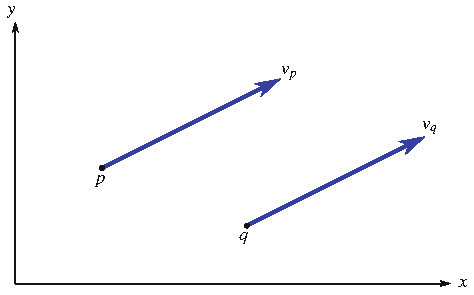
\includegraphics[width=0.562\linewidth]{images/vector/fig-10-1.pdf}
  \caption{向量 $2e_1+e_2$ 画在流形 $\mathbb{R}^2$ 中的两个不同点 $p$ 和 $q$ 处. 这两个向量以直观明显的方式彼此平行}
  \label{fig:10-1}
\end{figure}

正如我们以前讨论过的，$S^2$ 是一个流形，因为 $S^2$ 的每个点的小邻域看起来都像 $\mathbb{R}^2$. 然而，考虑图~\ref{fig:10-2} 所示的 $S^2$，其中点 $p$ 是``北极''，点 $q$ 在``赤道''上. 现在考虑 $v_p\in T_pS^2$. $T_qS^2$ 中什么样的向量可以在某种意义上被认为是与 $v_p$ 平行的？也就是说，把 $v_p$ 平行移动到点 $q$ 的结果是什么？从图~\ref{fig:10-2} 中显然看不出这一点. 事实证明，为了找到流形上向量的平行移动，需要在流形上添加某种附加结构. 这种附加结构称为\newterm{connection}{联络}{connection}. 它本质上是一种``连接''邻近切空间的方式（无论``邻近''意味着什么！）. 联络超出了本书的范围，但它们在流形理论中起着至关重要的作用. 在一般流形上，我们必须显式地指定一个联络，而在欧几里得空间流形上，联络已经隐含地建立在我们对欧几里得空间的直观理解之中. 一般流形与欧几里得空间流形 $\mathbb{R}^n$ 之间的这一重大差别，正是我们如此小心翼翼地区分两者的原因之一.

\begin{figure}[htbp]
  \centering
  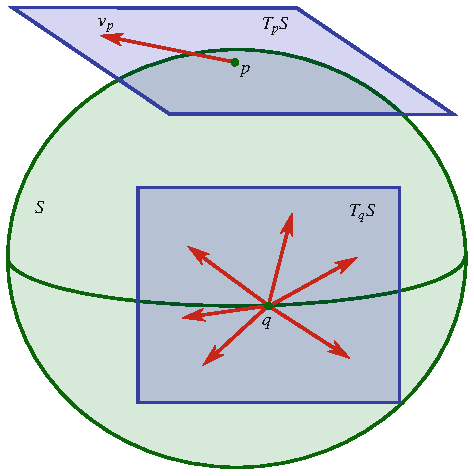
\includegraphics[width=0.562\linewidth]{images/vector/fig-10-2.pdf}
  \caption{向量 $v_p$，其中 $p$ 是``北极''. ``赤道''上点 $q$ 处的向量中有哪些与 $v_p$ 平行？}
  \label{fig:10-2}
\end{figure}

现在考虑图~\ref{fig:10-3} 所示的 $\mathbb{R}^2$ 中的点 $p$ 和 $q$. 关于两点之间的直线应该是什么样子，有一个非常自然且直观的想法. 而且，给定笛卡尔坐标系，我们知道如何测量两点之间的距离. 我们还知道环面 $T^2$ 是一个流形，因为 $T^2$ 的每个点的非常小的邻域看起来都像 $\mathbb{R}^2$. 然而，环面上点 $p$ 与 $q$ 之间的``直线''会是什么样子？在这种情形下``直线''究竟意味着什么？从图~\ref{fig:10-4} 中看不出这一点. 再退一步讲，人们如何测量环面上两点之间的距离？要回答这个问题，除了联络之外，还需要流形上一种称为\newterm{metric}{度量}{metric}的结构. 我们稍后实际上会多了解一点度量，不过不会深入. 总之，在一般流形上，我们必须显式地指定一个度量，而在欧几里得空间流形上，一个称为欧几里得度量的度量已经隐含地建立在我们对欧几里得空间的直观理解之中. 这是一般流形与我们熟悉的欧几里得空间流形 $\mathbb{R}^n$ 之间的另一个重大差别，也是我们必须谨慎区分两者的又一个原因.

\begin{figure}[htbp]
  \centering
  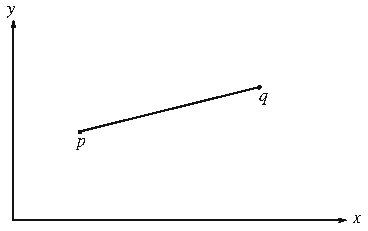
\includegraphics[width=0.436\linewidth]{images/vector/fig-10-3.pdf}
  \caption{流形 $\mathbb{R}^2$ 中两点 $p$ 与 $q$ 之间的一条直线. 直线在欧几里得空间中意味着什么是自然而直观的.}
  \label{fig:10-3}
\end{figure}

\begin{figure}[htbp]
  \centering
  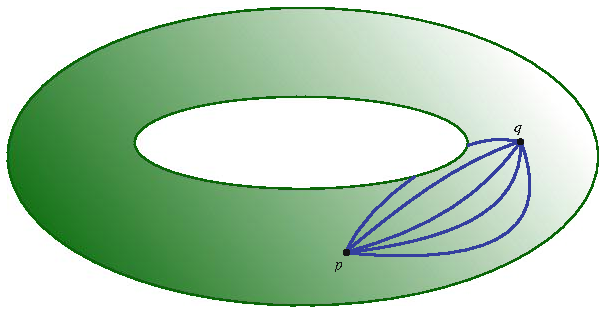
\includegraphics[width=0.721\linewidth]{images/vector/fig-10-4.pdf}
  \caption{环面 $T^2$，其上标出了两个点 $p$ 和 $q$. 图中画出了连接这两点的几条线. 连接流形 $T^2$ 上两点的``直线''会是什么样子？在这种情形下``直线''究竟意味着什么？}
  \label{fig:10-4}
\end{figure}

所有这一切都突显了一般流形与你所熟悉的欧几里得空间流形 $\mathbb{R}^n$ 之间的真正差别. 然而，在我们所做的一切中，我们都费了功夫区分``流形''$\mathbb{R}^n$ 与流形的切空间，后者基本上就是向量空间 $\mathbb{R}^n$. 既然你已经习惯了这一点，转向一般流形的情况应该不会太难.

现在我们准备给可微流形一个严格的定义. 在这里我们将坚持所谓的\newterm{differentiable-manifold}{微分流形}{differentiable manifold}. 实际上有很多不同类型的流形具有不同的性质. 由于这不是流形理论课程，我们将坚持最简单的那种. 一般流形保留欧几里得空间流形的一些结构，但不会保留欧几里得空间流形的联络或欧几里得度量.

\begin{definition}[$n$ 维流形]\label{def:10-1-1}
$n$ 维流形是一个空间 $M$，它可被一族局部\newterm{coordinate-neighborhood}{坐标邻域}{coordinate neighborhood} $U_i$ 连同一一映射 $\phi_i:U_i\to\mathbb{R}^n$ 完全覆盖，这些映射称为\newterm{coordinate-map}{坐标映射}{coordinate map}. $U_i$ 与 $\phi_i$ 合起来称为\newterm{coordinate-patch}{坐标片}{coordinate patch}或\newterm{chart}{坐标图}{chart}，一般记为 $(U_i,\phi_i)$. 所有坐标图合在一起 $\{(U_i,\phi_i)\}$ 称为 $M$ 的坐标系或\newterm{atlas}{图册}{atlas}. 由于 $U_i$ 覆盖整个 $M$，我们写 $M=\bigcup U_i$. 又因 $\phi_i$ 是一一的，它可逆，所以 $\phi_i^{-1}$ 存在且良定义. 最后，若两个坐标图有非空交集 $U_i\cap U_j\neq\emptyset$，则函数 $\phi_j\circ\phi_i^{-1}:\mathbb{R}^n\to\mathbb{R}^n$ 称为\newterm{transition-function}{转移函数}{transition function}.
\end{definition}

这里有很多重要的术语，我们总结如下：
\[
\begin{array}{rcl}
U_i & : & \text{坐标邻域},\\
\phi_i:U_i\to\mathbb{R}^n & : & \text{坐标映射},\\
(U_i,\phi_i) & : & \text{坐标片/坐标图},\\
\left\{(U_i,\phi_i)\right\} & : & \text{坐标系/图册},\\
\phi_j\circ\phi_i^{-1}:\mathbb{R}^n\to\mathbb{R}^n & : & \text{转移函数}.
\end{array}
\]

图~\ref{fig:10-5} 给出了一个二维的例子. 图册和坐标图这两个词尤其具有启发性；世界的图册（atlas）不就是一本地图（chart）的集合吗？这里 chart 一词是表示地图的航海用语.

\begin{figure}[htbp]
  \centering
  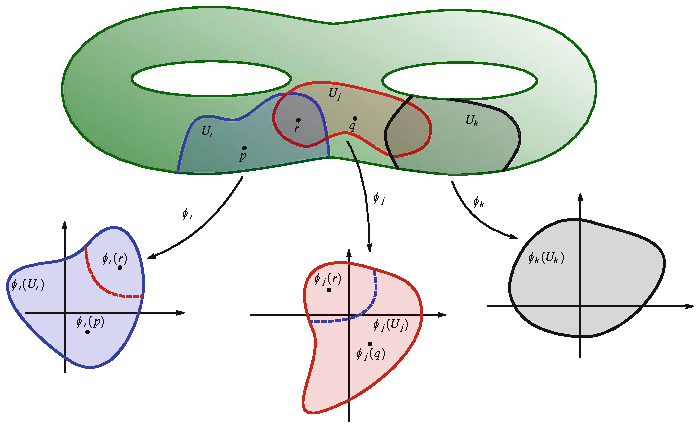
\includegraphics[width=0.960\linewidth]{images/vector/fig-10-5.pdf}
  \caption{这里展示了一个二维流形——双环面，连同三个坐标图 $(U_i,\phi_i)$、$(U_j,\phi_j)$ 和 $(U_k,\phi_k)$. 注意点 $r\in U_i\cap U_j$. 显然 $\phi_j\circ\phi_i^{-1}$ 把 $\phi_i(U_i\cap U_j)\subset\mathbb{R}^2$ 送到 $\phi_j(U_i\cap U_j)\subset\mathbb{R}^2$}
  \label{fig:10-5}
\end{figure}

现在考虑当点 $r\in U_i\cap U_j\neq\emptyset$ 时会发生什么. 我们有 $\phi_i(r)\in\mathbb{R}^n$ 和 $\phi_j(r)\in\mathbb{R}^n$. 此外，$\phi_j\circ\phi_i^{-1}$ 把 $\phi_i(U_i\cap U_j)\subset\mathbb{R}^n$ 送到 $\phi_j(U_i\cap U_j)\subset\mathbb{R}^n$，也就是说，$\phi_j\circ\phi_i^{-1}$ 是 $\mathbb{R}^n$ 的一个子集到 $\mathbb{R}^n$ 的另一个子集的映射，因此以 $\phi_i(U_i\cap U_j)$ 为定义域、以 $\phi_j(U_i\cap U_j)$ 为值域的映射 $\phi_j\circ\phi_i^{-1}:\mathbb{R}^n\to\mathbb{R}^n$，是我们知道如何从多元微积分求导的那种映射.

\begin{definition}[微分流形]\label{def:10-1-2}
微分流形是一个集合 $M$，连同坐标图族 $(U_i,\phi_i)$，其中 $M=\bigcup U_i$，使得每个映射 $\phi_j\circ\phi_i^{-1}$（其中 $U_i\cap U_j\neq\emptyset$）都是可微的.
\end{definition}

让我们看一个简单的显式例子，看看这是如何运作的. 考虑 $\mathbb{R}^2$ 中的单位圆 $S^1$. 我们将证明 $S^1$ 确实是一个微分流形. 令 $U_1$ 是 $S^1$ 中由 $0<t<2\pi$ 的点 $(\cos t,\sin t)$ 组成的子集. 那么由 $(\cos t,\sin t)\mapsto t$ 定义的 $\phi_1:U_1\to\mathbb{R}$ 是到开区间 $(0,2\pi)\subset\mathbb{R}$ 上的一一映射，所以 $(U_1,\phi_1)$ 是 $S^1$ 上的一个坐标图. 见图~\ref{fig:10-6}.

\begin{figure}[htbp]
  \centering
  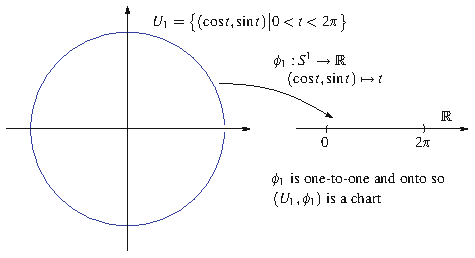
\includegraphics[width=0.582\linewidth]{images/vector/fig-10-6.pdf}
  \caption{$S^1$ 上的坐标图 $(U_1,\phi_1)$. $U_1$ 是 $S^1$ 中由 $0<t<2\pi$ 的点 $(\cos t,\sin t)$ 组成的子集，$\phi_1:U_1\to\mathbb{R}$ 由 $(\cos t,\sin t)\mapsto t$ 定义}
  \label{fig:10-6}
\end{figure}

类似地，令 $U_2$ 是 $S^1$ 中由 $-\pi<\tau<\pi$ 的点 $(\cos\tau,\sin\tau)$ 组成的子集. 那么由 $(\cos\tau,\sin\tau)\mapsto\tau$ 定义的 $\phi_2:U_2\to\mathbb{R}$ 是到 $\mathbb{R}$ 的某个子集上的一一映射，所以 $(U_2,\phi_2)$ 是 $S^1$ 上的另一个坐标图. 见图~\ref{fig:10-7}. 定义域 $U_1$ 和 $U_2$ 覆盖整个 $S^1$，即 $S^1=U_1\cup U_2$. 我们说 $(U_1,\phi_1)$ 和 $(U_2,\phi_2)$ 是 $S^1$ 的一个图册.

\begin{figure}[htbp]
  \centering
  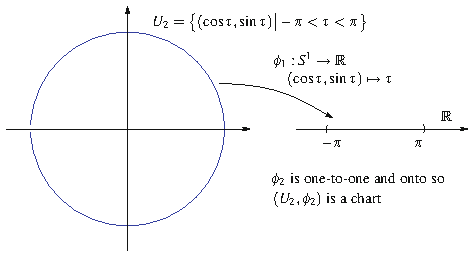
\includegraphics[width=0.582\linewidth]{images/vector/fig-10-7.pdf}
  \caption{$S^1$ 上的坐标图 $(U_2,\phi_2)$. $U_2$ 是 $S^1$ 中由 $-\pi<\tau<\pi$ 的点 $(\cos\tau,\sin\tau)$ 组成的子集，$\phi_2:U_2\to\mathbb{R}$ 由 $(\cos\tau,\sin\tau)\mapsto\tau$ 定义}
  \label{fig:10-7}
\end{figure}

\begin{question}\label{q:10-1}
$S^1$ 的哪个点不在 $U_1$ 中？$S^1$ 的哪个点不在 $U_2$ 中？为什么这些点没有被包含？它们能被包含进去吗？即使它们被包含进去了，仍然会出现什么问题？
\end{question}

注意 $U_1\cap U_2$ 有两个连通分支，即 $S^1$ 的上半开半圆和下半开半圆. 见图~\ref{fig:10-8}. 在上半开半圆上，对 $0<t<\pi$ 有 $\phi_1^{-1}\circ\phi_2(t)=t$，这是可微的；在下半开半圆上，对 $\pi<t<2\pi$ 有 $\phi_1^{-1}\circ\phi_2(t)=t-2\pi$，这也是可微的. 因此 $S^1$ 是一个微分流形.

\begin{figure}[htbp]
  \centering
  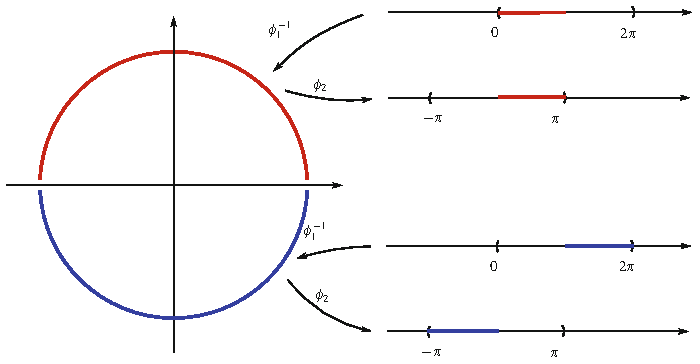
\includegraphics[width=0.867\linewidth]{images/vector/fig-10-8.pdf}
  \caption{$U_1\cap U_2$ 有两个连通分支：$S^1$ 的上半开半圆（红色）和下半开半圆（蓝色）. 在上半开半圆上，对 $0<t<\pi$ 有 $\phi_1^{-1}\circ\phi_2(t)=t$；在下半开半圆上，对 $\pi<t<2\pi$ 有 $\phi_1^{-1}\circ\phi_2(t)=t-2\pi$. 这两者都是可微的，使 $S^1$ 成为一个微分流形}
  \label{fig:10-8}
\end{figure}

在大多数微分几何教科书中，此时通常会出现可定向流形和带边流形的定义. 根据第 1.2 节你已经知道体积带有符号. 定向流形的思想与此相关，它本质上是指流形带有一种判断体积何时为正、何时为负的方式. 我们将在第 10.4 节讨论流形上的积分时讨论定向流形. 带边流形本质上就是你想象中的那种流形，即带有某种边界或``边缘''的流形. 什么是边界或``边缘''可以非常精确地用坐标图来定义. 在本书中我们不会显式地讨论带边流形，不过在第 11 章我们将在 Stokes 定理的具体语境中更仔细地探讨边界的某些概念.

\section{流形的切空间}

回想一下，我们之前引入切空间时，是通过考虑流形 $\mathbb{R}^n$ 来做的. 我们考虑的例子有 $n=2$ 或 $3$，但这个思想对任意 $n$ 都成立. 见图~\ref{fig:2-14} 至图~\ref{fig:2-17}. 我们选取一个点 $p\in\mathbb{R}^n$，然后考虑从该点出发的所有向量 $v_p$. 我们把从点 $p$ 出发的所有向量 $v_p$ 的集合称为 $\mathbb{R}^n$ 在 $p$ 处的切空间，记为 $T_p\mathbb{R}^n$. 然后我们看到 $T_p\mathbb{R}^n$ 本质上与向量空间 $\mathbb{R}^n$ 是同一个空间. 本节我们想给出切空间的一种稍微更抽象的表述.

例如，给定一个一般流形 $M$，你可能想知道我们说从点 $p\in M$ 发出的向量是什么意思. 毕竟，$\mathbb{R}^n$ 除了是微分流形之外，显然也是一个向量空间，这使我们能够谈论向量，而一般微分流形根本不需要是向量空间，这意味着流形中没有任何向量. 考虑图~\ref{fig:10-9} 所示的球面 $S^2\subset\mathbb{R}^3$. 我们可以在点 $p\in S^2$ 处画出各种各样与 $S^2$ 相切的向量，但这些向量实际上在空间 $\mathbb{R}^3$ 中——即流形 $S^2$ 所嵌入的空间——而不是在流形 $S^2$ 本身之中.

\begin{figure}[htbp]
  \centering
  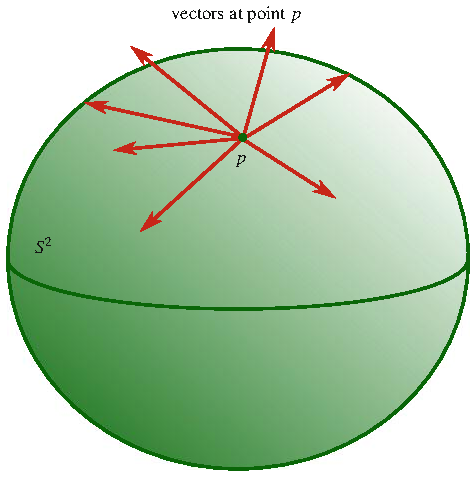
\includegraphics[width=0.564\linewidth]{images/vector/fig-10-9.pdf}
  \caption{流形 $S^2$ 连同点 $p$ 处若干个与 $S^2$ 相切的向量. 然而，这些向量实际上不在 $S^2$ 中. 它们事实上在 $\mathbb{R}^3$ 中，即我们为了画 $S^2$ 而把 $S^2$ 嵌入其中的那个空间}
  \label{fig:10-9}
\end{figure}

当我们最初引入切空间时，我们通过画几个流形并说点 $p$ 处的切空间本质上就是流形在该点的切平面（或超平面）来说明切空间的一般思想. 例如，图~\ref{fig:10-10} 中画出了流形 $S^2$ 连同它的几个切平面.

\begin{figure}[htbp]
  \centering
  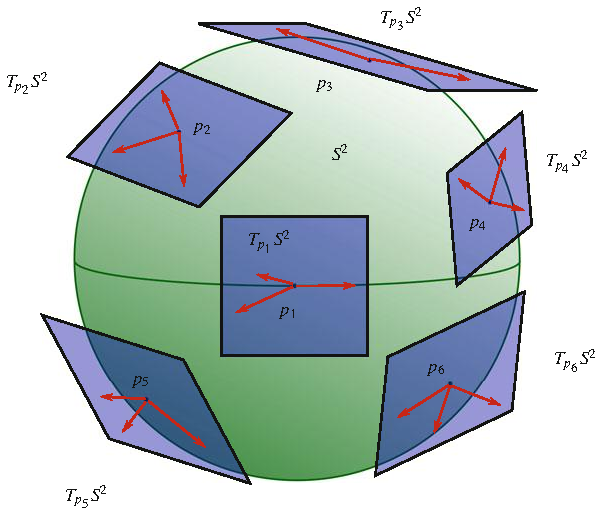
\includegraphics[width=0.850\linewidth]{images/vector/fig-10-10.pdf}
  \caption{当我们引入流形 $S^2$ 的切空间概念时，我们画出了流形在流形上各个点处的切平面. 实际上 $S^2$ 的每个点都有这样一个切平面}
  \label{fig:10-10}
\end{figure}

这是一个非常好的漫画式图画，有助于我们可视化和理解切空间，我们将继续使用它，但它要求我们的流形嵌入到某个 $\mathbb{R}^n$ 中，切空间也嵌入其中，就像 $S^2$ 和 $S^2$ 的切空间都嵌入 $\mathbb{R}^3$ 一样. 根据微分几何中一个深刻的定理——Whitney 嵌入定理，任何足够好的流形都可以嵌入到足够大的 $n$ 的 $\mathbb{R}^n$ 中，这意味着我们实际上可以继续使用我们的漫画式图画来帮助可视化和思考切空间. 然而，要以这种方式可视化切空间，我们实质上必须``走出''流形. 要求我们``走出''流形才能思考或定义它的性质称为\newterm{extrinsic-property}{外蕴性质}{extrinsic property}.

\begin{figure}[htbp]
  \centering
  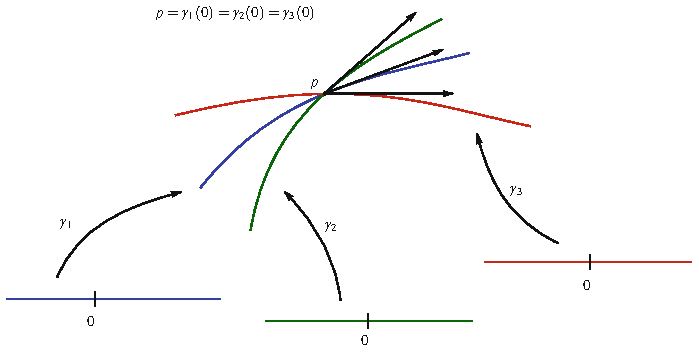
\includegraphics[width=0.865\linewidth]{images/vector/fig-10-11.pdf}
  \caption{三条曲线 $\gamma_i:(-\epsilon,\epsilon)\subset\mathbb{R}\longrightarrow M$（$i=1,2,3$），使得 $\gamma_i(0)=p$. 每条曲线在点 $p$ 处都有一个切向量}
  \label{fig:10-11}
\end{figure}

我们希望能够在不必``走出''流形的情况下定义和思考切空间. 在很多情况下，能够``留在流形内部''思考流形的性质是有用的. 我们可以在``留在流形内部''的同时定义或思考的流形性质称为\newterm{intrinsic-property}{内蕴性质}{intrinsic property}. 内蕴性质绝不需要或依赖于流形嵌入到某个 $\mathbb{R}^n$ 中. 尽管到目前为止我们一直在从外蕴的角度思考切向量和切空间，但它们实际上是内蕴性质. 我们可以在``留在流形内部''的同时定义它们和思考它们. 当我们这样做时，从点发出的箭头的想法就不再合适了.

我们将通过首先考虑所有满足 $\gamma(0)=p\in M$ 的\newterm{smooth-curve}{光滑曲线}{smooth curve}
\[
\gamma:(-\epsilon,\epsilon)\subset\mathbb{R}\longrightarrow M
\]
来接近切向量的内蕴定义，其中 $\epsilon$ 只是某个小的正数. 在图~\ref{fig:10-11} 中我们画了几条光滑曲线 $\gamma_i:(-\epsilon,\epsilon)\to M$，其中对所有 $i$ 都有 $\gamma_i(0)=p$. 我们把 $\gamma_i$ 所依赖的参数称为时间. 不去深究光滑曲线的技术含义，只需假定它意味着你直观上认为的那个意思，即曲线上没有尖角.

每个切向量 $v_p$ 实际上都与某条经过点 $p\in M$ 的光滑曲线相切. 但是，虽然切向量 $v_p$ 可能实际上只存在于 $M$ 所嵌入的空间 $\mathbb{R}^n$ 中，曲线 $\gamma$ 却完全存在于流形 $M$ 之中. 本质上，这些曲线中的每一条都在点 $p$ 处定义了一个不同的切向量. 因此，一般的思想是把流形 $M$ 在点 $p$ 处的切向量与流形中经过点 $p$ 的曲线等同起来，从而不再需要把 $M$ 嵌入到某个更大的空间 $\mathbb{R}^n$ 中就能拥有切向量.

看起来似乎 $M$ 的切空间可能等价于满足 $\gamma(0)=p$ 的曲线 $\gamma:(-\epsilon,\epsilon)\to M$ 的集合. 这几乎是对的，但不完全对. 有两个问题我们必须仔细考虑. 为处理第一个问题，考虑图~\ref{fig:10-12}. 这里有三条不同的曲线 $\gamma_1,\gamma_2,\gamma_3:(-\epsilon,\epsilon)\to M$，满足 $\gamma_1(0)=\gamma_2(0)=\gamma_3(0)=p$，它们在非常靠近 $p$ 的地方是相同的. 如果两条曲线在非常靠近 $p$ 的地方是相同的，那么我们能否在某种意义下认为它们是同一条曲线？乍一看这样做似乎是合理的.

\begin{figure}[htbp]
  \centering
  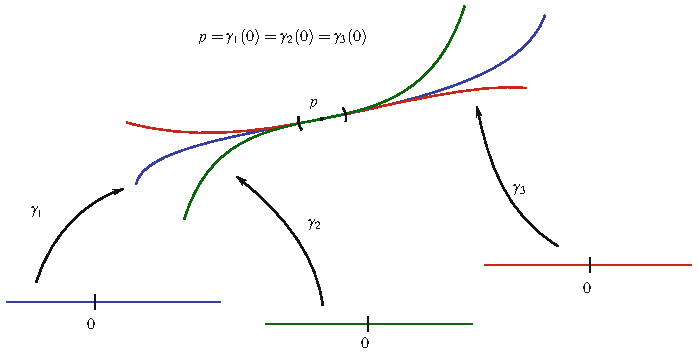
\includegraphics[width=0.829\linewidth]{images/vector/fig-10-12.pdf}
  \caption{与图~\ref{fig:10-11} 一样，三条曲线 $\gamma_i:(-\epsilon,\epsilon)\subset\mathbb{R}\longrightarrow M$（$i=1,2,3$），使得 $\gamma_i(0)=p$. 不过，这里当我们非常靠近 $p$ 时，这些曲线是相同的}
  \label{fig:10-12}
\end{figure}

为考虑第二个问题，考虑 $T_pM$ 中的向量 $v_p$ 和 $2v_p$. 从图~\ref{fig:10-13} 来看，$v_p$ 和 $2v_p$ 都可以由同一条曲线 $\gamma$ 表示. 问题是，当我们使用曲线时，如何区分 $T_pM$ 中的向量 $v_p$ 和 $2v_p$？它们指向相同的方向，但第二个向量是第一个向量的两倍长.

\begin{figure}[htbp]
  \centering
  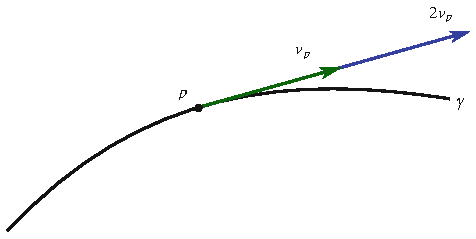
\includegraphics[width=0.564\linewidth]{images/vector/fig-10-13.pdf}
  \caption{两个向量 $v_p$ 和 $2v_p$，它们看起来都与同一条曲线 $\gamma$ 相切}
  \label{fig:10-13}
\end{figure}

处理这第二个问题的线索在于，我们把 $\gamma$ 所依赖的参数称为时间. $\gamma$ 在时间 $t=0$ 处的导数给出时间 $0$ 处的速度. 当我们提高沿曲线 $\gamma$ 运动的速率时，速度更大，因而速度向量变得更长. 因此，为了区分 $v_p$ 和 $2v_p$，参数化的速度被提高，使其在 $t=0$ 处是原来的两倍.

让我们考虑一个简单的例子. 令 $M=\mathbb{R}_{xy}^2$ 为以 $x$ 和 $y$ 参数化的欧几里得平面. 考虑 $\mathbb{R}_{xy}^2$ 的原点处的下列三个向量：
\[
u_0=\binom{1}{2},\qquad v_0=2u_0=\binom{2}{4},\qquad w_0=-u_0=\binom{-1}{-2}.
\]

见图~\ref{fig:10-14}. 这些向量由下列三条曲线 $\alpha,\beta,\gamma:(-\epsilon,\epsilon)\to\mathbb{R}_{xy}^2$ 给出，其中
\[
\begin{aligned}
\alpha(t)&=\bigl(\alpha_1(t),\alpha_2(t)\bigr)=(t,2t),\\
\beta(t)&=\bigl(\beta_1(t),\beta_2(t)\bigr)=(2t,4t),\\
\gamma(t)&=\bigl(\gamma_1(t),\gamma_2(t)\bigr)=(-t,-2t).
\end{aligned}
\]

尽管在 $\mathbb{R}^2$ 中画出曲线 $\alpha$、$\beta$ 和 $\gamma$ 看起来像是同一条曲线，严格地说它们都是不同的曲线，因为它们的参数化不同.

\begin{figure}[htbp]
  \centering
  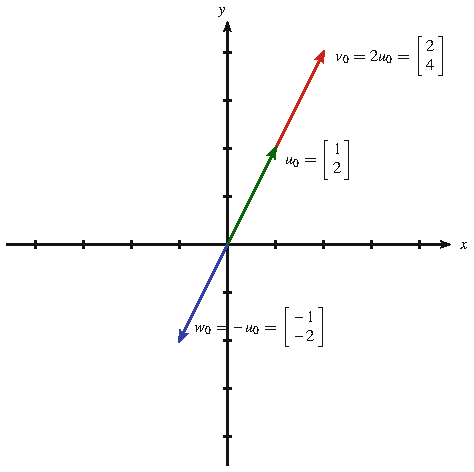
\includegraphics[width=0.562\linewidth]{images/vector/fig-10-14.pdf}
  \caption{流形 $\mathbb{R}_{xy}^2$，原点处有三个向量 $u_0=[1,2]^T$、$v_0=2u_0=[2,4]^T$ 和 $w_0=-u_0=[-1,-2]^T$. 这三个向量由具有不同参数化的三条曲线 $\alpha$、$\beta$ 和 $\gamma$ 确定}
  \label{fig:10-14}
\end{figure}

现在我们将用 $M$ 上的曲线来定义 $M$ 在点 $p$ 处的切空间 $T_pM$，但我们必须把上述两个问题考虑进去. 如图~\ref{fig:10-12} 那样，在非常靠近 $p$ 的地方相同的两条曲线，在靠近 $p$ 的地方有相同的值域. 如果两条曲线在靠近 $p$ 处有相同的值域，并且在靠近 $p$ 处有相同的参数化，则称它们等价，记为 $\sim$. 假设 $\gamma_1$、$\gamma_2$ 和 $\gamma_3$ 在靠近 $p$ 处都有相同的值域，并且在靠近 $p$ 处都有相同的参数化，那么我们说 $\gamma_1\sim\gamma_2\sim\gamma_3$.

\begin{definition}[曲线的等价类]\label{def:10-2-1}
所有等价曲线的集合称为\newterm{equivalence-class}{等价类}{equivalence class}. $\gamma_1$ 的等价类是与 $\gamma_1$ 等价的所有曲线的集合，记为 $[\gamma_1]$，定义为
\[
[\gamma_1]\equiv\left\{\gamma\mid\gamma\sim\gamma_1\right\}.
\]
\end{definition}

因此，若 $\gamma_1\sim\gamma_2\sim\gamma_3$，则有 $[\gamma_1]=[\gamma_2]=[\gamma_3]$. 这意味着用等价类中的哪个成员来表示该等价类并不重要.

\begin{definition}[切空间]\label{def:10-2-2}
点 $p$ 处曲线的每个等价类被定义为 $p$ 处的一个切向量. 当我们想指出基点是 $p$ 时，我们写 $[\gamma]_p$. $M$ 在 $p$ 处的切空间被定义为点 $p$ 处所有切向量（即曲线的等价类）的集合，
\[
T_pM=\left\{[\gamma]_p\mid\gamma:(-\epsilon,\epsilon)\to M\text{ 且 }\gamma(0)=p\right\}.
\]
\end{definition}

因此，流形 $M$ 在点 $p$ 处的切空间是经过 $p\in M$ 的所有曲线的等价类的集合. 注意，切空间的这个定义是内蕴的，它完全依赖于流形 $M$ 中经过点 $p$ 的曲线. 因此我们不需要``走出''流形就能可视化或思考切空间. 这个定义独立于我们的流形所嵌入的任何更大的空间.

现在我们要理解向量的外蕴观点与内蕴观点之间的关系. 实际位于我们的流形所嵌入的空间中的向量 $v_p$，是某条曲线 $\gamma$ 在点 $p$ 处的速度向量，所以我们做了等同 $v_p=[\gamma]_p$. 要从曲线 $\gamma$ 重新得到向量 $v_p$，我们必须对时间求 $\gamma$ 的导数，并在时间 $t=0$ 处求值. 基本上，我们是在求映射 $\gamma:(-\epsilon,\epsilon)\to M$ 的 Jacobian 矩阵.

回到我们的具体例子，我们有
\[
u_{(0,0)}\equiv[\alpha]_{(0,0)},\qquad v_{(0,0)}\equiv[\beta]_{(0,0)},\qquad w_{(0,0)}\equiv[\gamma]_{(0,0)}.
\]

但请注意，尽管当我们把曲线画在 $\mathbb{R}^2$ 上时，它们在我们的图画中看起来都是``同一条''曲线，但它们实际上是不同的曲线，因为它们的参数化不同，所以不属于同一个曲线等价类. 换言之，我们有 $\alpha\nsim\beta$、$\alpha\nsim\gamma$ 和 $\beta\nsim\gamma$. 通常我们只简单地用 $0$ 表示基点 $(0,0)$，但由于我们想强调基点与在时间 $t=0$ 处对偏导数求值之间的区别，这里我们要对记号格外小心. 我们可以看到我们关于向量的两种观点是如何相互关联的，
\begin{align*}
u_{(0,0)}\equiv\left[\left(\alpha_1(t),\alpha_2(t)\right)\right]_{(0,0)}=\left[(t,2t)\right]_{(0,0)}, \\
u_{(0,0)}=\begin{bmatrix}\left.\dfrac{\partial\alpha_1(t)}{\partial t}\right|_{t=0}\\[1.2em] \left.\dfrac{\partial\alpha_2(t)}{\partial t}\right|_{t=0}\end{bmatrix}_{(0,0)}=\begin{bmatrix}\left.\dfrac{\partial(t)}{\partial t}\right|_{t=0}\\[1.2em] \left.\dfrac{\partial(2t)}{\partial t}\right|_{t=0}\end{bmatrix}_{(0,0)}=\binom{1}{2}_{(0,0)}.
\end{align*}
类似地，我们有
\begin{align*}
v_{(0,0)}\equiv\left[\left(\beta_1(t),\beta_2(t)\right)\right]_{(0,0)}=\left[(2t,4t)\right]_{(0,0)}, \\
v_{(0,0)}=\begin{bmatrix}\left.\dfrac{\partial\beta_1(t)}{\partial t}\right|_{t=0}\\[1.2em] \left.\dfrac{\partial\beta_2(t)}{\partial t}\right|_{t=0}\end{bmatrix}_{(0,0)}=\begin{bmatrix}\left.\dfrac{\partial(2t)}{\partial t}\right|_{t=0}\\[1.2em] \left.\dfrac{\partial(4t)}{\partial t}\right|_{t=0}\end{bmatrix}_{(0,0)}=\binom{2}{4}_{(0,0)},
\end{align*}
以及
\begin{align*}
w_{(0,0)}\equiv\left[\left(\gamma_1(t),\gamma_2(t)\right)\right]_{(0,0)}=\left[(-t,-2t)\right]_{(0,0)}, \\
w_{(0,0)}=\begin{bmatrix}\left.\dfrac{\partial\gamma_1(t)}{\partial t}\right|_{t=0}\\[1.2em] \left.\dfrac{\partial\gamma_2(t)}{\partial t}\right|_{t=0}\end{bmatrix}_{(0,0)}=\begin{bmatrix}\left.\dfrac{\partial(-t)}{\partial t}\right|_{t=0}\\[1.2em] \left.\dfrac{\partial(-2t)}{\partial t}\right|_{t=0}\end{bmatrix}_{(0,0)}=\binom{-1}{-2}_{(0,0)}.
\end{align*}

下面是我们在流形上定义向量的两种方式之间进行转换的钥匙. 等价类定义基于完全存在于我们的流形 $M$ 内部的曲线，不需要把 $M$ 嵌入到更大的环境空间就能``看到''向量；我们的向量只是被看作完全位于 $M$ 中的曲线. 我在这里将称之为向量定义的方式，需要把我们的流形 $M$ 嵌入到环境空间 $\mathbb{R}^n$ 中，或者在一点处画出流形 $M$ 的切空间，才能``看到''向量. 在等价类定义中，我们把曲线看作向量；在向量定义中，我们把曲线的导数看作向量. 这在你看来可能很奇怪，但这只是从两个不同的视角思考向量而已. 希望这不会太令人困惑.

\[
\begin{array}{c|c|c}
\hline
\text{等价类定义} & \Longleftrightarrow & \underline{\text{向量定义}}\\
\hline
v_p=[\gamma]_p,\quad p=\gamma(0) & & v_p=[\gamma']_p=[\gamma]_p'\\
=\left[\left(\gamma_1(t),\ldots,\gamma_n(t)\right)\right] & & =\left[\left(\gamma_1'(t),\ldots,\gamma_n'(t)\right)\right]_p\\
& & =\left[\left(\gamma_1(t),\ldots,\gamma_n(t)\right)\right]_p'\\
& & =\begin{bmatrix}\gamma_1'(t=0)\\ \vdots\\ \gamma_n'(t=0)\end{bmatrix}_p\\
& & =\begin{bmatrix}\left.\dfrac{\partial\gamma_1(t)}{\partial t}\right|_{t=0}\\[1.2em] \vdots\\[0.6em] \left.\dfrac{\partial\gamma_n(t)}{\partial t}\right|_{t=0}\end{bmatrix}_p\\
\hline
\end{array}
\]

这里还要再说一句. 如我们所知，积分在某种意义上与微分相反. 如果我们能把向量 $v_p$ 看作曲线 $\gamma$ 在点 $p$ 处的导数，那么我们能否把曲线 $\gamma$ 看作向量 $v_p$ 的积分？这里的问题是 $v_p$ 只存在于单独一个点处，而在一个点处积分的想法是定义不清的. 为了做积分，我们需要在某个点周围有一个光滑向量场. 不去深究光滑向量场的技术细节，把它想成一个随着点变化而光滑变化的向量场即可. 一旦我们在某个邻域中有了一个光滑向量场，我们就可以谈论称为积分曲线的曲线了. 用来表示某个向量 $v_p$ 的等价类 $[\gamma]_p$ 的曲线 $\gamma$ 不必是积分曲线，但如果 $v_p$ 是光滑向量场的一个元素，那么人们通常会做出一个未言明的假设：$\gamma$ 是一条积分曲线. 我们将在第 12 章和附录 B 中在电磁学和几何力学的语境下更详细地讨论积分曲线.

回想一下，在第 2.3 节中，我们把点 $p$ 处的切向量与方向导数等同起来. 通过这样做，我们把切空间的欧几里得基向量与偏微分算子等同起来. 换言之，我们找到了下列等同，
\[
e_{1p}=\left.\frac{\partial}{\partial x}\right|_p,\qquad e_{2p}=\left.\frac{\partial}{\partial y}\right|_p,\qquad e_{3p}=\left.\frac{\partial}{\partial z}\right|_p.
\]

因此，对于向量 $v_p\in T_p\mathbb{R}^3$，
\[
v_p=\begin{bmatrix}v_1\\v_2\\v_3\end{bmatrix}_p=v_1e_{1p}+v_2e_{2p}+v_3e_{3p}=v_1\left.\frac{\partial}{\partial x}\right|_p+v_2\left.\frac{\partial}{\partial y}\right|_p+v_3\left.\frac{\partial}{\partial z}\right|_p.
\]

考虑 $\gamma:(-\epsilon,\epsilon)\to M$（其中 $\gamma(0)=p$）和 $f:M\to\mathbb{R}$. 那么 $f\circ\gamma:(-\epsilon,\epsilon)\subset\mathbb{R}\to\mathbb{R}$，如图~\ref{fig:10-15} 所示. 函数 $f:\mathbb{R}^3\to\mathbb{R}$ 在方向 $v_p$ 上的方向导数被写为向量 $v_p$ 作用在函数 $f$ 上，
\[
v_p[f]=\left(v_1\left.\frac{\partial}{\partial x}\right|_p+v_2\left.\frac{\partial}{\partial y}\right|_p+v_3\left.\frac{\partial}{\partial z}\right|_p\right)[f]=v_1\left.\frac{\partial f}{\partial x}\right|_p+v_2\left.\frac{\partial f}{\partial y}\right|_p+v_3\left.\frac{\partial f}{\partial z}\right|_p.
\]

\begin{figure}[htbp]
  \centering
  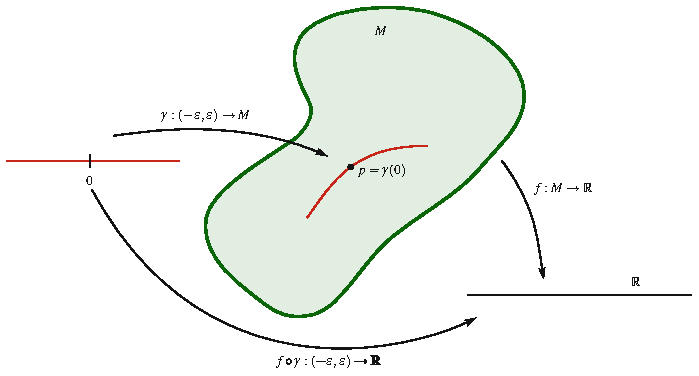
\includegraphics[width=0.960\linewidth]{images/vector/fig-10-15.pdf}
  \caption{由 $\gamma:(-\epsilon,\epsilon)\to M$（其中 $\gamma(0)=p$）给出的向量 $[\gamma]_p$ 以及函数 $f:M\to\mathbb{R}$. 于是有 $f\circ\gamma:(-\epsilon,\epsilon)\subset\mathbb{R}\to\mathbb{R}$，这是我们知道如何求导的那种映射}
  \label{fig:10-15}
\end{figure}

我们想在更抽象的、向量 $v_p$ 由曲线等价类 $[\gamma]_p$ 给出的内蕴背景中考虑这是什么，即当我们有 $v_p\equiv[\gamma]_p$ 时. 以前我们用记号 $v_p[f]$ 表示 $D_{v_p}f$，即 $f$ 在 $v_p$ 方向上的方向导数. 我们用这个记号来强调这样一个事实：在某种意义上，正是向量 $v_p$ 在作用在函数 $f$ 上. 只要我们把向量写成 $v_p$，我们就继续使用这个记号；但当我们用曲线等价类记号 $[\gamma]_p$ 写向量时，写 $[\gamma]_p[f]$ 就有点奇怪了，因为两组方括号 $[\cdot]$ 有不同的含义. 记号有时与习惯和约定一样多的是理性规划的结果.

当我们的向量 $v_p$ 由曲线等价类 $[\gamma]_p$ 给出时，$f$ 在 $v_p$ 方向上的方向导数由下式给出，
\[
\begin{aligned}
v_p[f]=D_{[\gamma]_p}f&=[f\circ\gamma]_p'\\
&=\left.\frac{\partial(f\circ\gamma)}{\partial t}\right|_{t=0}\\
&=\lim_{h\to 0}\frac{(f\circ\gamma)(h)-(f\circ\gamma)(0)}{h}.
\end{aligned}
\]

一个常用的记号是 $D_{[\gamma]_p}f$，它模仿多元微积分中通常使用的记号. $D_{[\gamma]_p}f$ 的其他记号包括 $[(f\circ\gamma)']_p$、$[f\circ\gamma]_p'$、$[(f\circ\gamma)']_{t=0}$ 甚至 $[f\circ\gamma]_{t=0}'$. 没有一种完全标准的写法，你可以在记号中使用各种不同的变体. 当然关键之处在于，如果向量在点 $p=\gamma(0)$ 处，那就意味着 $\gamma$ 的导数必须在 $t=0$ 处求值. 这才是要点. 此外，通常人们只写一个 $0$. 你需要根据语境来判断 $0$ 是指在 $t=0$ 处求值，还是基点是原点 $(0,0)$. 发出这个警告之后，我们就不再试图如此精确了.

注意，$f$ 在点 $p=\gamma(0)$ 处沿方向 $[\gamma]_p$ 的方向导数被定义为与一元函数 $f\circ\gamma$ 在 $t=0$ 处的普通导数相同的东西. 很容易看出，用这个记号我们会得到相同的答案. 假设 $\gamma(t)=\bigl(x(t),y(t),z(t)\bigr)$，于是有
\[
v_p=\left[\bigl(x(t),y(t),z(t)\bigr)\right]_p'=\begin{bmatrix}x'(t=0)\\ y'(t=0)\\ z'(t=0)\end{bmatrix}_p.
\]
利用 $f\circ\gamma(t)=f\bigl(x(t),y(t),z(t)\bigr)$，我们进而得到
\[
\begin{aligned}
v_p[f]=D_{[\gamma]_p}f&=\left.\frac{\partial(f\circ\gamma)}{\partial t}\right|_{t=0}\\
&=\left.\frac{\partial f\bigl(x(t),y(t),z(t)\bigr)}{\partial t}\right|_0\\
&=\left.\frac{\partial f}{\partial x}\right|_{\gamma(0)}\cdot\left.\frac{\partial x}{\partial t}\right|_0+\left.\frac{\partial f}{\partial y}\right|_{\gamma(0)}\cdot\left.\frac{\partial y}{\partial t}\right|_0+\left.\frac{\partial f}{\partial z}\right|_{\gamma(0)}\cdot\left.\frac{\partial z}{\partial t}\right|_0\qquad\text{链式法则}\\
&=\left.\frac{\partial f}{\partial x}\right|_p\underbrace{x'(0)}_{v_1}+\left.\frac{\partial f}{\partial y}\right|_p\underbrace{y'(0)}_{v_2}+\left.\frac{\partial f}{\partial z}\right|_p\underbrace{z'(0)}_{v_3},
\end{aligned}
\]
这与上面我们得到的 $v_p[f]$ 完全一样，只是记号中去掉了基点 $p$.

回到一个具体的例子，假设我们有函数 $f:\mathbb{R}_{xy}^2\to\mathbb{R}$，由 $f(x,y)=x+\sin(y)$ 给出. 我们想求 $u_0[f]$，其中 $u_0=\binom{1}{2}=[(t,2t)]_0$. （注意，这里我们有 $0=(0,0)$.）像以前那样进行，我们有
\[
\begin{aligned}
u_0[f]&=\left(1\cdot\left.\frac{\partial}{\partial x}\right|_0+2\cdot\left.\frac{\partial}{\partial y}\right|_0\right)f\\
&=1\cdot\left.\frac{\partial\bigl(x+\sin(y)\bigr)}{\partial x}\right|_0+2\cdot\left.\frac{\partial\bigl(x+\sin(y)\bigr)}{\partial y}\right|_0\\
&=1\cdot 1+2\cdot\cos(0)\\
&=3.
\end{aligned}
\]
然而，用 $u_0=[\gamma]_0=\left[(t,2t)\right]_0$，我们有
\[
\begin{aligned}
D_{u_0}f=[f\circ\gamma]_0'&=\left.\frac{\partial(f\circ\gamma)}{\partial t}\right|_0\\
&=\left.\frac{\partial\bigl(t+\sin(2t)\bigr)}{\partial t}\right|_0\\
&=\left.1+2\cos(2t)\right|_0\\
&=1+2=3.
\end{aligned}
\]

这一切看起来都很好，直到你注意到在我们的例子中，我们的流形是 $\mathbb{R}_{xy}^2$，即``内置''了笛卡尔坐标系的 $\mathbb{R}^2$. 求复合 $f\circ\gamma$ 依赖于知道这个坐标系. 为什么？因为函数 $f$ 是显式地用变量 $x$ 和 $y$ 写出来的，这使得写出 $f\circ\gamma$ 很容易. 但是在一个没有``内置''很好标准坐标系的流形上，我们如何处理方向导数呢？换言之，如果写出 $f\circ\gamma$ 实际上是什么并不那么直截了当，那该怎么办？

如果我们想求 $f:M\to\mathbb{R}$ 在点 $p\in M$ 处沿方向 $v_p\equiv[\gamma]_p$ 的导数，那么我们需要知道如何复合 $f$ 和 $\gamma$，得到映射 $f\circ\gamma:(-\epsilon,\epsilon)\subset\mathbb{R}\to\mathbb{R}$. 但对于任意流形 $M$，这实际上可能并不清楚. 复合 $f\circ\gamma$ 实际上依赖于某个坐标图 $\phi$. 因此，我们的复合 $f\circ\gamma$ 必须借助某个坐标图来完成，以便我们能处理从 $\mathbb{R}^n$ 到 $\mathbb{R}^m$ 的映射，这是我们理解的. 考虑图~\ref{fig:10-16}. 由于微分流形带有坐标图 $(U,\phi)$，我们可以利用它们. 我们有
\[
f\circ\gamma=f\circ\phi^{-1}\circ\phi\circ\gamma.
\]

\begin{figure}[htbp]
  \centering
  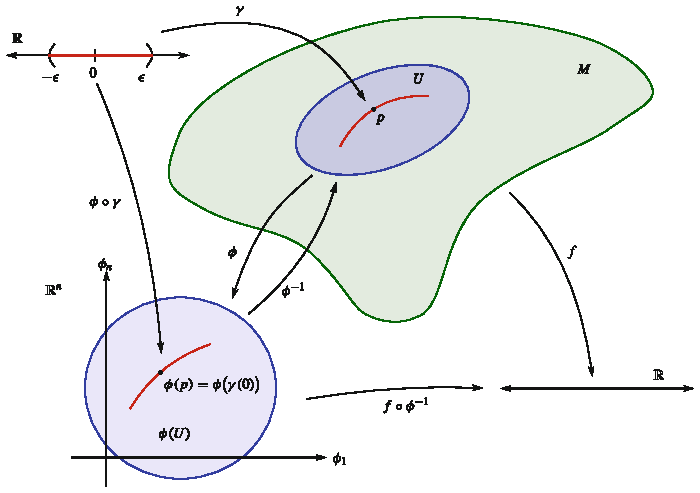
\includegraphics[width=0.960\linewidth]{images/vector/fig-10-16.pdf}
  \caption{这里展示了流形 $M$ 以及三样东西：(a) 表示点 $p$ 处切向量的曲线 $\gamma$，(b) 流形 $M$ 上的实值函数 $f:M\to\mathbb{R}$，(c) 满足 $p\in U$ 的坐标图 $(U,\phi)$. 显然有 $f\circ\gamma=f\circ\phi^{-1}\circ\phi\circ\gamma=(f\circ\phi^{-1})\circ(\phi\circ\gamma)$. 图中还画出了映射 $\phi\circ\gamma:\mathbb{R}\to\mathbb{R}^n$ 和 $f\circ\phi^{-1}:\mathbb{R}^n\to\mathbb{R}$}
  \label{fig:10-16}
\end{figure}

映射 $\phi\circ\gamma:(-\epsilon,\epsilon)\subset\mathbb{R}\to\phi(U)\subset\mathbb{R}^n$ 是我们实际上可以计算并求导的那种映射，映射 $f\circ\phi^{-1}:\phi(U)\subset\mathbb{R}^n\to\mathbb{R}$ 也是如此. 所以我们实际上有
\[
\begin{aligned}
v_p[f]=D_{[\gamma]_p}f&=[f\circ\gamma]_0'\\
&=[f\circ\phi^{-1}\circ\phi\circ\gamma]_0'\\
&=[f\circ\phi^{-1}]_{\phi(p)}'\cdot[\phi\circ\gamma]_0'\\
&=\left.\frac{\partial(f\circ\phi^{-1})}{\partial\phi}\right|_{\phi(p)}\cdot\left.\frac{\partial(\phi\circ\gamma)}{\partial t}\right|_0.
\end{aligned}
\]

注意我们得到
\begin{center}
\fbox{\parbox{0.92\textwidth}{\centering
曲线情形的链式法则：\\[0.4em]
$[f\circ\phi^{-1}\circ\phi\circ\gamma]_0'=[f\circ\phi^{-1}]_{\phi\circ\gamma(0)}'\cdot[\phi\circ\gamma]_0'=[f\circ\phi^{-1}]_{\phi(p)}'\cdot[\phi\circ\gamma]_0'.$
}}
\end{center}

这实际上就是链式法则的一种写法. 它看起来可能一点也不像你习惯的链式法则，但这就是链式法则在这个语境中的样子——当我们使用向量的曲线等价类定义来求导时.

为证明这一点，让我们分别考虑这些项中的每一项. 首先我们来看映射
\[
\begin{array}{c}
\phi\circ\gamma:(-\epsilon,\epsilon)\subset\mathbb{R}\longrightarrow\phi(U)\subset\mathbb{R}^n\\
t\longmapsto\Bigl(\phi_1\bigl(\gamma(t)\bigr),\phi_2\bigl(\gamma(t)\bigr),\ldots,\phi_n\bigl(\gamma(t)\bigr)\Bigr)\\
=\Bigl(\phi_1\circ\gamma(t),\phi_2\circ\gamma(t),\ldots,\phi_n\circ\gamma(t)\Bigr)
\end{array}
\]
所以 $\left.\frac{\partial(\phi\circ\gamma)}{\partial t}\right|_0$ 实际上是在 $t=0$ 处求值的 Jacobian 矩阵，
\[
\left.\frac{\partial(\phi\circ\gamma)}{\partial t}\right|_0=\begin{bmatrix}\left.\dfrac{\partial(\phi_1\circ\gamma)}{\partial t}\right|_0\\[1.2em] \left.\dfrac{\partial(\phi_2\circ\gamma)}{\partial t}\right|_0\\[1.2em] \vdots\\[0.6em] \left.\dfrac{\partial(\phi_n\circ\gamma)}{\partial t}\right|_0\end{bmatrix}.
\]

接下来我们来看映射
\[
\begin{array}{c}
f\circ\phi^{-1}:\phi(U)\subset\mathbb{R}^n\longrightarrow\mathbb{R}\\
(\phi_1,\phi_2,\ldots,\phi_n)\longmapsto f\bigl(\phi^{-1}(\phi_1,\phi_2,\ldots,\phi_n)\bigr)\\
=f\circ\phi^{-1}(\phi_1,\phi_2,\ldots,\phi_n)
\end{array}
\]
所以 $\left.\frac{\partial(f\circ\phi^{-1})}{\partial\phi}\right|_{\phi(p)}$ 实际上是在 $\phi(p)$ 处求值的 Jacobian 矩阵，
\[
\left.\frac{\partial(f\circ\phi^{-1})}{\partial\phi}\right|_{\phi(p)}=\left[\left.\frac{\partial(f\circ\phi^{-1})}{\partial\phi_1}\right|_{\phi(p)},\left.\frac{\partial(f\circ\phi^{-1})}{\partial\phi_2}\right|_{\phi(p)},\ldots,\left.\frac{\partial(f\circ\phi^{-1})}{\partial\phi_n}\right|_{\phi(p)}\right].
\]

把这两部分合在一起，我们有
\[
\begin{aligned}
D_{[\gamma]_p}f&=\left[\left.\frac{\partial(f\circ\phi^{-1})}{\partial\phi_1}\right|_{\phi(p)},\left.\frac{\partial(f\circ\phi^{-1})}{\partial\phi_2}\right|_{\phi(p)},\ldots,\left.\frac{\partial(f\circ\phi^{-1})}{\partial\phi_n}\right|_{\phi(p)}\right]\begin{bmatrix}\left.\dfrac{\partial(\phi_1\circ\gamma)}{\partial t}\right|_0\\[1.2em] \left.\dfrac{\partial(\phi_2\circ\gamma)}{\partial t}\right|_0\\[1.2em] \vdots\\[0.6em] \left.\dfrac{\partial(\phi_n\circ\gamma)}{\partial t}\right|_0\end{bmatrix}\\
&=\left.\frac{\partial(f\circ\phi^{-1})}{\partial\phi_1}\right|_{\phi(p)}\left.\frac{\partial(\phi_1\circ\gamma)}{\partial t}\right|_0+\cdots+\left.\frac{\partial(f\circ\phi^{-1})}{\partial\phi_n}\right|_{\phi(p)}\left.\frac{\partial(\phi_n\circ\gamma)}{\partial t}\right|_0\\
&=\sum_{i=1}^{n}\left.\frac{\partial(f\circ\phi^{-1})}{\partial\phi_i}\right|_{\phi(p)}\left.\frac{\partial(\phi_i\circ\gamma)}{\partial t}\right|_0.
\end{aligned}
\]

还要注意，这意味着
\[
[f\circ\phi^{-1}]_{\phi(p)}'\cdot[\phi\circ\gamma]_0'=\sum_{i=1}^{n}\left.\frac{\partial(f\circ\phi^{-1})}{\partial\phi_i}\right|_{\phi(p)}\left.\frac{\partial(\phi_i\circ\gamma)}{\partial t}\right|_0,
\]
这清楚地表明 $[f\circ\phi^{-1}]_{\phi(p)}'\cdot[\phi\circ\gamma]_0'$ 确实只是链式法则的另一种写法.

\begin{question}\label{q:10-2}
假设 $(U,\phi)$ 和 $(\widetilde{U},\widetilde{\phi})$ 是 $M$ 上的两个坐标图，$p\in U\cap\widetilde{U}$，$\gamma:(-\epsilon,\epsilon)\subset\mathbb{R}\to M$ 满足 $\gamma(0)=p$，且 $f$ 是 $M$ 上的实值函数. 证明
\[
\left.\frac{\partial(f\circ\phi^{-1}\circ\phi\circ\gamma)}{\partial t}\right|_0=\left.\frac{\partial(f\circ\widetilde{\phi}^{-1}\circ\widetilde{\phi}\circ\gamma)}{\partial t}\right|_0.
\]
\end{question}

\section{流形上的前推与拉回}

我们在第 6 章已经讨论过前推和拉回. 我们仔细考察过的例子之一是变量替换公式 $f:\mathbb{R}_{xy}^2\to\mathbb{R}_{uv}^2$，其中 $f(x,y)=\bigl(u(x,y),v(x,y)\bigr)=(x+y,x-y)$. 我们找到了 $f$ 的前推是映射
\[
T_pf\equiv f_*\equiv D_pf:T_p\mathbb{R}_{xy}^2\longrightarrow T_{f(p)}\mathbb{R}_{uv}^2,
\]
它由 Jacobian 矩阵
\[
T_pf\equiv f_*\equiv D_pf=\begin{bmatrix}\dfrac{\partial u}{\partial x}&\dfrac{\partial u}{\partial y}\\[0.6em] \dfrac{\partial v}{\partial x}&\dfrac{\partial v}{\partial y}\end{bmatrix}_p
\]
给出.

更一般地，给定两个流形之间的映射 $f:M\to N$，这个映射 $f$ 诱导出另一个映射 $Tf:TM\to TN$，它把 $M$ 的切丛送到 $N$ 的切丛. 在特定点 $p\in M$ 处，我们有 $T_pf:T_pM\to T_pN$. 这个映射把向量 $v_p\in T_pM$ 前推到向量 $T_pf\cdot v_p\in T_{f(p)}N$. 见图~\ref{fig:10-17}.

\begin{figure}[htbp]
  \centering
  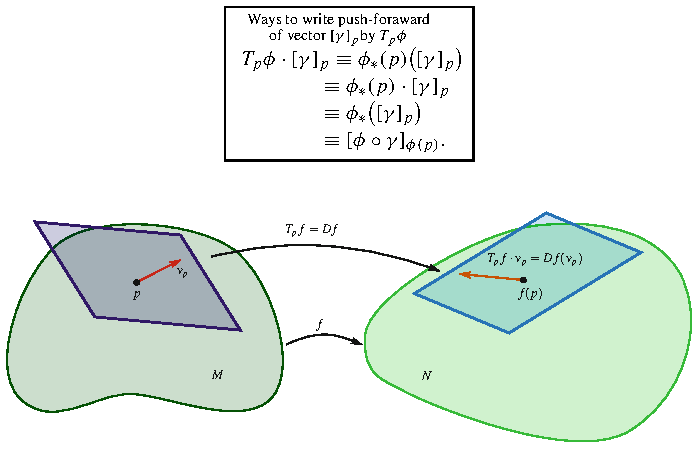
\includegraphics[width=0.830\linewidth]{images/vector/fig-10-17.pdf}
  \caption{给定流形之间的映射 $f:M\to N$，则 $f$ 诱导出前推映射 $Tf:TM\to TN$. 在特定点处，我们有 $T_pf:T_pM\to T_pN$}
  \label{fig:10-17}
\end{figure}

现在我们想从更抽象的角度来看这个. 假设我们有映射 $\phi:M\to N$，并且我们有一个由曲线 $\gamma$ 确定的向量 $v_p$. 我们想知道 $T_p\phi\cdot v_p$ 是什么. 从图~\ref{fig:10-18} 应该清楚，由映射 $\phi$ 对向量 $[\gamma]$ 的前推是曲线 $\phi\circ\gamma$. 于是我们把 $[\gamma]_p$ 被 $T_p\phi$ 的前推定义为
\begin{center}
\fbox{\parbox{0.92\textwidth}{\centering
向量 $[\gamma]_p$ 被 $T_p\phi$ 的前推：\\[0.4em]
$T_p\phi\cdot[\gamma]_p=[\phi\circ\gamma]_{\phi(p)}.$
}}
\end{center}

在很多方面，这是前推的一个更简洁的表述. 它也使抽象计算简单得多，我们将看到这一点. 在记法上，有几种不同的写法，它们都表示同一件事.

\begin{center}
\fbox{\parbox{0.92\textwidth}{\centering
写向量 $[\gamma]_p$ 被 $T_p\phi$ 前推的方式：\\[0.4em]
$T_p\phi\cdot[\gamma]_p\equiv\phi_*(p)\left([\gamma]_p\right)\equiv\phi_*(p)\cdot[\gamma]_p\equiv\phi_*\left([\gamma]_p\right)\equiv[\phi\circ\gamma]_{\phi(p)}.$
}}
\end{center}

\begin{figure}[htbp]
  \centering
  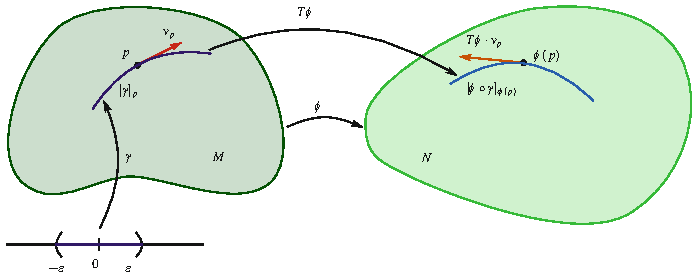
\includegraphics[width=0.960\linewidth]{images/vector/fig-10-18.pdf}
  \caption{这里我们有一个流形之间的映射 $\phi:M\to N$ 和一个向量 $[\gamma]_p\in T_pM$，其中 $\gamma:(-\epsilon,\epsilon)\to M$ 满足 $\gamma(0)=p$. 这个向量被 $T_p\phi$ 前推是什么？它就是由曲线 $\phi\circ\gamma$ 给出的向量，即 $[\phi\circ\gamma]_{\phi(p)}$}
  \label{fig:10-18}
\end{figure}

当然，所有这些记号也都可以省去基点来写：
\[
T\phi\cdot[\gamma]\equiv\phi_*([\gamma])\equiv\phi_*\cdot[\gamma]=[\phi\circ\gamma].
\]

回到我们熟悉的例子 $\phi:\mathbb{R}_{xy}^2\to\mathbb{R}_{uv}^2$，其中 $\phi(x,y)=\bigl(u(x,y),v(x,y)\bigr)=(x+y,x-y)$，我们可以看到计算一个向量的前推的这两种方式给出相同的答案. 再次考虑向量 $u_0=\binom{1}{2}\equiv[\gamma]_0$，其中
\[
\gamma:(-\epsilon,\epsilon)\longrightarrow\mathbb{R}_{xy}^2,\qquad t\longmapsto(t,2t).
\]

我们希望求 $u_0$ 被 $\phi$ 的前推. 首先我们通过求切映射 $T\phi$ 来做，然后利用它来求 $T\phi\cdot u_0$.
\[
T\phi=\phi_*=\begin{bmatrix}\dfrac{\partial u}{\partial x}&\dfrac{\partial u}{\partial y}\\[0.6em] \dfrac{\partial v}{\partial x}&\dfrac{\partial v}{\partial y}\end{bmatrix}=\begin{bmatrix}1&1\\1&-1\end{bmatrix}.
\]
我们不为这个矩阵担心基点，因为显然 $T\phi$ 不依赖于它所处的基点. 然后我们求 $u_0$ 的前推：
\[
T\phi\cdot u_0=\begin{bmatrix}1&1\\1&-1\end{bmatrix}\binom{1}{2}_{\phi(0)}=\binom{3}{-1}_0.
\]

现在我们用更抽象的向量曲线等价类定义来计算同样的东西：
\[
T\phi\cdot[\gamma]_0=[\phi\circ\gamma]_{\phi(0)}=[\phi\circ(t,2t)]_0=[(t+2t,t-2t)]_0=[(3t,-t)]_0.
\]

因此曲线 $\phi\circ\gamma=(3t,-t)$ 就是我们要找的前推向量. 也就是说，$T\phi\cdot u_0\equiv[(3t,-t)]_0$. 为了检验我们的答案是正确的，并且与上面得到的答案等价，我们必须对时间求这条曲线的导数：
\[
[\phi\circ\gamma]_{\phi(0)}'=\begin{bmatrix}\left.\dfrac{\partial(\phi\circ\gamma)_1(t)}{\partial t}\right|_{t=0}\\[1.2em] \left.\dfrac{\partial(\phi\circ\gamma)_2(t)}{\partial t}\right|_{t=0}\end{bmatrix}_{\phi(0)}=\begin{bmatrix}\left.\dfrac{\partial(3t)}{\partial t}\right|_{t=0}\\[1.2em] \left.\dfrac{\partial(-t)}{\partial t}\right|_{t=0}\end{bmatrix}_{\phi(0)}=\binom{3}{-1}_0,
\]
这正是我们想证明的.

\begin{question}\label{q:10-3}
对映射 $\phi:M\to N$ 和函数 $f:N\to\mathbb{R}$，证明 $v_p[f\circ\phi]=\left(T_p\phi\cdot v_p\right)_{\phi(p)}[f]$.
\end{question}

现在我们已经解决了向量的前推，我们想来看微分形式的拉回. 概念上，发生的事情并不难理解. 相关的映射定义为
\begin{align*}
\phi:M\longrightarrow N,\qquad p\longmapsto\phi(p) \\
T_p\phi:T_pM\longrightarrow T_{\phi(p)}N,\qquad v_p\longmapsto T_p\phi\cdot v_p,\qquad [\gamma]_p\longmapsto[\phi\circ\gamma]_{\phi(p)} \\
T_p^*M\longleftarrow T_{\phi(p)}^*N:T_p^*\phi,\qquad T_p^*\phi\cdot\alpha_{\phi(p)}\longleftarrow\alpha_{\phi(p)}
\end{align*}
并在图~\ref{fig:10-19} 中示出. 1-形式 $\alpha_{\phi(p)}\in T_{\phi(p)}^*N$ 的拉回是 $T_p^*\phi\cdot\alpha_{\phi(p)}\in T_p^*M$，它因此吃向量 $v_p\in T_pM$. 于是我们把 1-形式的拉回定义为
\[
\left(T_p^*\phi\cdot\alpha_{\phi(p)}\right)(v_p)\equiv\alpha_{\phi(p)}\left(T_p\phi\cdot v_p\right).
\]

\begin{figure}[htbp]
  \centering
  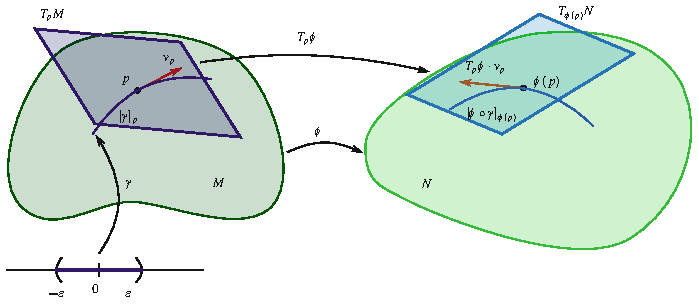
\includegraphics[width=0.960\linewidth]{images/vector/fig-10-19.pdf}
  \caption{这里说明了向量的前推与 1-形式的拉回之间的关系. 我们把余切空间 $T_p^*M$ 和 $T_{\phi(p)}^*N$ 画在切空间的上方，尽管切空间和余切空间都``附着''在流形的同一点上. 注意拉回映射与前推映射的方向相反}
  \label{fig:10-19}
\end{figure}

还要回想一下，给拉回映射标下标的是值域中的点 $p$，而不是定义域中的点. 这是一个相当不寻常的记法约定，但鉴于上面的定义，它使拉回与前推映射之间的联系显而易见. 利用我们在本节中引入的向量的曲线等价类定义，我们有拉回
\begin{center}
\fbox{\parbox{0.92\textwidth}{\centering
1-形式 $\alpha_{\phi(p)}$ 被 $T_p^*\phi$ 的拉回：\\[0.4em]
$\left(T_p^*\phi\cdot\alpha_{\phi(p)}\right)([\gamma]_p)\equiv\alpha_{\phi(p)}\left(T_p\phi\cdot[\gamma]_p\right)=\alpha_{\phi(p)}\left([\phi\circ\gamma]_{\phi(p)}\right).$
}}
\end{center}

这个等式用更传统的记号写起来实际上看起来非常简单. 这里我们省去基点来写拉回，这样你就能看到它实际上有多简单：
\begin{center}
\fbox{\parbox{0.92\textwidth}{\centering
$\phi^*\alpha([\gamma])=\alpha([\phi\circ\gamma]).$
}}
\end{center}

类似地，对于 $k$-形式 $\omega_{\phi(p)}\in\bigwedge_{\phi(p)}^k(N)$，我们得到拉回映射
\[
\bigwedge_p^k(M)\longleftarrow\bigwedge_{\phi(p)}^k(N):T_p^*\phi,\qquad T_p^*\phi\cdot\omega_{\phi(p)}\longleftarrow\omega_{\phi(p)},
\]
它定义为
\[
\left(T_p^*\phi\cdot\omega_{\phi(p)}\right)(v_{p_1},v_{p_2},\ldots,v_{p_k})\equiv\omega_{\phi(p)}\left(T_p\phi\cdot v_{p_1},T_p\phi\cdot v_{p_2},\ldots,T_p\phi\cdot v_{p_k}\right).
\]

用向量的曲线等价类定义，$k$-形式 $\omega$ 的拉回由下式给出，
\begin{center}
\fbox{\parbox{0.92\textwidth}{\centering
$k$-形式 $\omega_{\phi(p)}$ 被 $T_p^*\phi$ 的拉回：\\[0.4em]
$\left(T_p^*\phi\cdot\omega_{\phi(p)}\right)([\gamma_1]_p,[\gamma_2]_p,\ldots,[\gamma_k]_p)\equiv\omega_{\phi(p)}\left(T_p\phi\cdot[\gamma_1]_p,T_p\phi\cdot[\gamma_2]_p,\ldots,T_p\phi\cdot[\gamma_k]_p\right)$\\[0.4em]
$=\omega_{\phi(p)}\left([\phi\circ\gamma_1]_{\phi(p)},[\phi\circ\gamma_2]_{\phi(p)},\ldots,[\phi\circ\gamma_k]_{\phi(p)}\right).$
}}
\end{center}

我们还给出 0-形式的拉回的定义. 回想一下，流形 $N$ 上的 0-形式只是实值函数 $f:N\to\mathbb{R}$. 函数的拉回正是你所期望的，
\begin{center}
\fbox{\parbox{0.92\textwidth}{\centering
0-形式 $f$ 被 $T_p^*\phi$ 的拉回：\\[0.4em]
$T_p^*\phi\cdot f\equiv(f\circ\phi)(p)=f(\phi(p)).$
}}
\end{center}

这个定义用传统记法、且不含基点时看起来非常简单：
\begin{center}
\fbox{\parbox{0.92\textwidth}{\centering
0-形式 $f$ 被 $\phi^*$ 的拉回：\\[0.4em]
$\phi^*\cdot f\equiv f\circ\phi.$
}}
\end{center}

事实上，我们在第 6.7 节证明第三个恒等式 $\phi^*d=d\phi^*$ 时已经看到并使用过这一点.

\section{流形上的微积分}

没有理由不把你微积分和向量微积分课程中学到的所有微积分都归为``流形上的微积分''. 在这些情形中，流形只是欧几里得空间 $\mathbb{R}^2$ 或 $\mathbb{R}^3$. 然而，当人们听到流形上的微积分这个短语，或者流形上的积分、甚至流形上的分析等替代短语时，一般的假设是流形比欧几里得空间更复杂，是我们在本章引入的那种流形，即带有一个由坐标图 $(U_i,\phi_i)$ 组成的图册的那种流形.

\subsection{流形上的微分}

微积分一词当然既意味着微分也意味着积分. 本节我们将对流形上的微分做几点宏观的评论. 下一小节以及下一章将集中讨论流形上的积分. 人们经常遇到流形上的三种不同的微分概念. 这三种概念的作用方式都略有不同.

\begin{enumerate}
  \item \newterm{exterior-derivative}{外微分}{exterior derivative}：这是我们在本书中研究的那种微分，我们在第 4 章已经大量考察过外微分. 外微分作用于微分形式. 当微分形式是 0-形式，换言之只是一个函数时，外微分与微积分中的方向导数相同. 正如我们在第 4.5 节看到的，在很实在的意义上，外微分是我们的一般微积分课程中方向导数思想的推广. 也正是这种微分版本给出了将在第 11 章证明的推广 Stokes 定理. 这个推广的 Stokes 定理是流形上积分的重要组成部分. 最后，在第 4.3 节我们证明了外微分算子的局部存在性与唯一性. 现在我们已经有了必要的概念，下面将证明外微分算子的整体存在性与唯一性.
  \item Lie 导数：Lie 导数作用于称为\newterm{tensor}{张量}{tensor}的对象上. 微分形式实际上是张量的一个子集，所以谈论微分形式的 Lie 导数也完全说得通. 而且，Lie 微分有一个非常好的几何意义，比外微分更容易可视化和理解. 我们将在附录 A 中引入张量，并在第 A.7 节讨论 Lie 导数. 在那里我们导出几个把外微分与 Lie 微分联系起来的公式. 事实上，其中一个公式被用来通过归纳法证明整体外微分公式，该公式在第 4.4.2 节曾从某种几何的角度讨论过.
  \item \newterm{covariant-derivative}{协变导数}{covariant derivative}：本书完全不会讨论协变导数，但它们依赖于联络的概念，我们曾在第 10.1 节开头非常简略地讨论过. 如前所述，联络是流形上的附加结构，它``连接''切空间，以便告诉我们向量从一个切空间到另一个切空间的平行移动是什么. 其基本思想是，知道不同切空间中什么样的向量构成平行向量，使我们能够测量当张量和形式的输入向量被平行移动时它们如何变化. 协变导数是我们一般微积分课程中方向导数的第二种推广方式.
\end{enumerate}

你应该认识到，在讨论 $\mathbb{R}^2$ 或 $\mathbb{R}^3$ 时，这三种导数概念同样有效. 只是在你入门微积分课程中，你只对函数感兴趣，而不关心微分形式或张量. 除此之外，在我们流形中内置了一个非常自然且直观可理解的 $\mathbb{R}^2$ 或 $\mathbb{R}^3$ 上的欧几里得联络. 由于这些考虑，在一般微积分课程中实际上从来不需要讨论各种微分概念，老式的方向导数就足够了. 到你在向量微积分中时，你实际上确实学习了外微分，但正如你在第 9 章学到的，外微分被冠以梯度、旋度和散度这些专门的名称. 换言之，外微分的本质被不同的词汇和避免引入形式的企图掩盖了. 这就是为什么一切都保持为向量的原因.

但在更一般、更抽象的背景下，我们需要关注这些不同的微分概念. 有大量的恒等式把这些不同的导数思想彼此联系起来. 所有这些都使得流形上的微积分这个主题比欧几里得空间 $\mathbb{R}^2$ 或 $\mathbb{R}^3$ 上的微积分要复杂得多. 流形上的微积分实际上开始进入微分几何的领域，而上面提到的所有思想实际上将构成微分几何入门课程的主题.

说了这些之后，我们现在把注意力转向在微分形式的语境中很重要的一些基础内容. 我们首先简要地回到我们在第 4.3 节结束的地方. 在那节中，我们取了我们希望外微分具有的四个性质，称之为公理，然后导出了外微分的一般公式. 第四条公理基本上说明，在 0-形式的情形中，外微分必须与方向导数相同，从而确保外微分实际上是方向导数的推广. 然后我们利用这些公理导出了外导数的一般公式. 一旦我们做到了这一点，并有了一个一般微分形式的外导数的单一公式，我们就知道外微分算子 $d$ 必须既存在又唯一.

花点时间仔细回顾一下第 4.3 节. 注意两件事. 第一，第四条公理说明，在局部坐标下，对每个函数 $f$，都有 $df=\sum\frac{\partial f}{\partial x_i}dx_i$. 第二，我们曾假设我们有一个 n-形式
\[
\alpha=\sum\alpha_{i_1\cdots i_n}dx_{i_1}\wedge\cdots\wedge dx_{i_n}.
\]
在这两种情形中，我们都隐式地依赖一个坐标系，而且在该节的语境中，我们隐式地依赖笛卡尔坐标系. 但一般流形没有单一坐标系，相反它有一个由坐标片 $(U_i,\phi_i)$ 组成的图册 $\{(U_i,\phi_i)\}$. 第 4.3 节所做的一切只适用于单个坐标片 $(U_i,\phi_i)$. 当然，同样的论证和计算可以在许多坐标片中的每一个上进行，但这一切只意味着，在许多坐标片中的每一个上，我们都找到了一个给出微分形式外导数的公式，只要该形式用那个特定坐标片的坐标写出即可.

现在我们证明外微分算子 $d$ 整体存在且唯一. 这意味着 $d$ 在整个流形 $M=\bigcup U_i$ 上存在且唯一. 在坐标片 $(U_i,\phi_i)$ 上，我们证明了外微分算子存在且唯一，现在我们把它标为 $d_{U_i}$. 我们在这个坐标片上定义整体微分算子 $d$ 为 $d=d_{U_i}$. 类似地，在坐标片 $(U_j,\phi_j)$ 上，我们证明了外微分算子存在且唯一，现在我们把它标为 $d_{U_j}$. 我们同样在这个坐标片上定义整体微分算子 $d$ 为 $d=d_{U_j}$. 问题是，如果 $U_i\cap U_j\neq\emptyset$ 会怎样？由于 $d_{U_i}$ 在 $U_i$ 上存在且唯一，而 $d_{U_j}$ 在 $U_j$ 上存在且唯一，那么在 $U_i\cap U_j$ 上我们必须有 $d_{U_i}=d_{U_j}=d$. 由于这在所有坐标片的交上都成立，所以我们有 $d$ 整体存在且唯一，即在 $M=\bigcup U_i$ 上成立.

\subsection{流形上的积分}

现在我们把注意力转向流形上的积分. 既然流形上微分有好几种不同的思想，你就不应奇怪流形上积分也有不同的思想. 这里我们将把自己限制在讨论流形上微分形式的积分.

为了使一切都能顺顺利利地进行，我们将假设流形是可定向的. 当流形不可定向时也有办法做积分，但我们不在这里讨论它们.

\begin{definition}[可定向流形]\label{def:10-4-1}
可定向的 n 维流形 $M$ 是在流形的每一点处都有一个不为零的 n-形式的流形. 换言之，若 $fdx_1\wedge\cdots\wedge dx_n$ 是 $M$ 上的一个 n-形式，则不存在 $p\in M$ 使得 $f(p)=0$. 这意味着对所有点 $p\in M$，要么 $f(p)>0$，要么 $f(p)<0$. 具有这一性质的形式称为\newterm{nowhere-zero-n-form}{无处为零的 n-形式}{nowhere-zero n-form}. 于是，所有无处为零的 n-形式的集合分成两个等价类，一个等价类由所有处处为正的无处为零的 n-形式组成，第二个等价类由所有处处为负的无处为零的 n-形式组成. 通过选择这两个等价类中的一个，我们就规定了所谓的流形的\newterm{orientation}{定向}{orientation}.
\end{definition}

我们可以把定向想成允许我们以一致的方式求流形上的体积. 或者，我们可以把定向想成允许我们以一致的方式给所有切空间定向. 流形 $\mathbb{R}^n$ 的标准定向是包含无处为零的 n-形式 $dx_1\wedge\cdots\wedge dx_n$ 的那个等价类. 这个定向常常被描述为由 $dx_1\wedge\cdots\wedge dx_n$ 诱导的定向.

但注意我们在这里做了什么. 只要我们的流形有一个由单个坐标图组成的图册，说流形 $M$ 具有由 n-形式 $dx_1\wedge\cdots\wedge dx_n$ 诱导的定向就一切顺利. 但如果不是这样呢？考虑图~\ref{fig:10-20}，其中我们展示了一个带两个坐标图 $(U_i,\phi_i)$ 和 $(U_j,\phi_j)$（其中 $U_i\cap U_j\neq\emptyset$）的流形. $U_i$ 上的\newterm{volume-form}{体积形式}{volume form}会是什么样子？让我们考虑定义在整个 $\mathbb{R}^n$ 上的标准体积形式 $dx_1\wedge\cdots\wedge dx_n$，因此它显然定义在 $\phi_i(U_i)\subset\mathbb{R}^n$ 上. 我们可以把这个标准体积形式拉回到 $U_i\subset M$ 上. 因此，在某种意义上，$T^*\phi_i\cdot\left(dx_1\wedge\cdots\wedge dx_n\right)$ 是 $U_i\subset M$ 上的一个``标准''体积形式.

\begin{figure}[htbp]
  \centering
  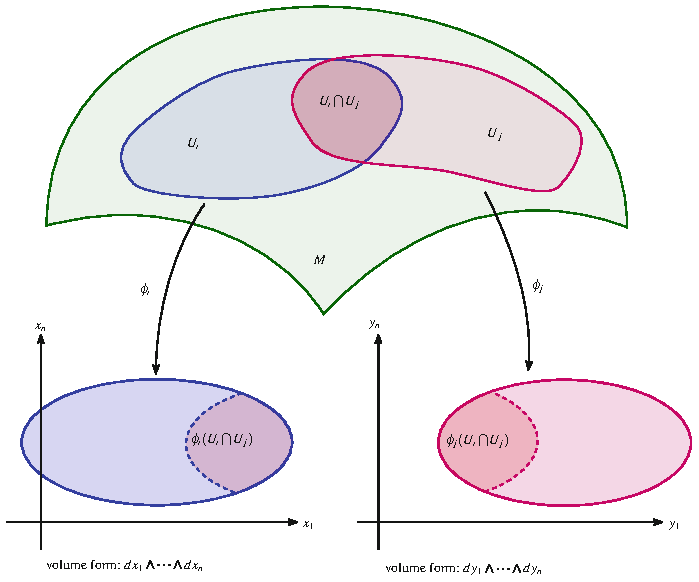
\includegraphics[width=0.952\linewidth]{images/vector/fig-10-20.pdf}
  \caption{带两个坐标图 $(U_i,\phi_i)$ 和 $(U_j,\phi_j)$（其中 $U_i\cap U_j\neq\emptyset$）的流形 $M$. $\mathbb{R}^n$ 的标准体积形式 $dx_1\wedge\cdots\wedge dx_n$ 在 $\phi_i(U_i)$ 和 $\phi_j(U_j)$ 上都存在}
  \label{fig:10-20}
\end{figure}

类似地，$U_j$ 上的体积形式会是什么样子？像以前一样，我们将考虑 $\phi_j(U_j)\subset\mathbb{R}^n$ 上的标准体积形式，为不把它与 $dx_1\wedge\cdots\wedge dx_n$ 混淆，我们称之为 $dy_1\wedge\cdots\wedge dy_n$. 我们可以把这个标准体积形式拉回到 $U_j\subset M$ 上，得到拉回 $T^*\phi_j\cdot\left(dy_1\wedge\cdots\wedge dy_n\right)$，作为 $U_j\subset M$ 上的一个``标准''体积形式. 这两个体积形式在它们都有定义的 $U_i\cap U_j$ 上如何相互关联？一般来说它们不会相同. 但要记住我们真正追求的是什么. 我们真正想要的是在整个 $M$ 上定义一个一致的体积形式 $\omega$，以便用它来定义 $M$ 上的定向.

在整个 $M$ 上寻找一个``一致的体积形式'' $\omega$ 实际上意味着什么？考虑图~\ref{fig:10-21}. 假设我们在 $\phi_j(U_j)$ 上有标准体积形式 $dy_1\wedge\cdots\wedge dy_n$. 如果 $\phi_i(U_i)$ 上存在一个体积形式 $f(x_1,\ldots,x_n)dx_1\wedge\cdots\wedge dx_n$，使得在 $U_i\cap U_j$ 上有
\[
T^*\phi_i\left(f(x_1,\ldots,x_n)dx_1\wedge\cdots\wedge dx_n\right)=T^*\phi_j\left(dy_1\wedge\cdots\wedge dy_n\right),
\]
那么我们就可以利用这两个体积形式（一个在 $U_j$ 上，一个在 $U_i$ 上）``缝合''出一个定义在 $U_i\cup U_j$ 上的体积形式. 通过反复这样做，我们可以``缝合''出一个定义在整个 $M$ 上的体积形式 $\omega$. 但首先我们需要在 $\phi_i(U_i)$ 上找到体积形式 $f(x_1,\ldots,x_n)dx_1\wedge\cdots\wedge dx_n$.

\begin{figure}[htbp]
  \centering
  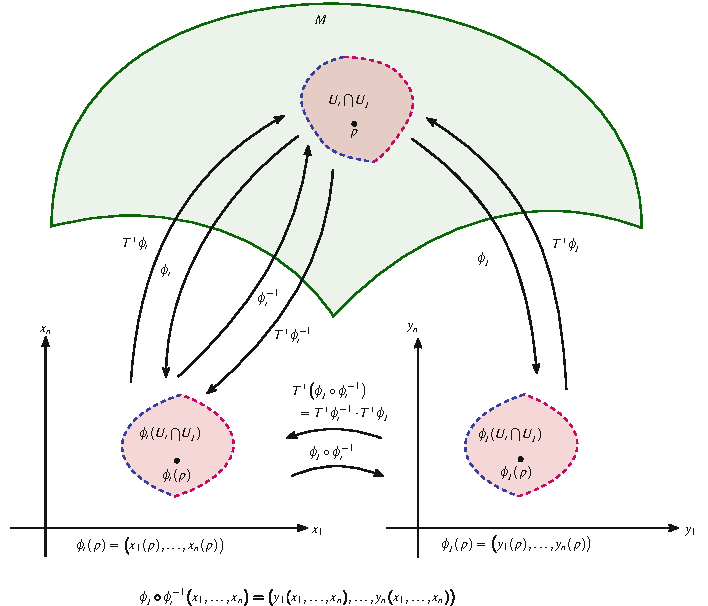
\includegraphics[width=0.949\linewidth]{images/vector/fig-10-21.pdf}
  \caption{这里我们聚焦于图~\ref{fig:10-20} 中的 $U_i\cap U_j$. 求 $T^*\left(\phi_j\circ\phi_i^{-1}\right)\left(dy_1\wedge\cdots\wedge dy_n\right)$ 所需的全部映射}
  \label{fig:10-21}
\end{figure}

看图~\ref{fig:10-21} 可以清楚看到，我们想要的等式
\[
T^*\phi_i\left(f(x_1,\ldots,x_n)dx_1\wedge\cdots\wedge dx_n\right)=T^*\phi_j\left(dy_1\wedge\cdots\wedge dy_n\right)
\]
等价于
\[
\begin{aligned}
f(x_1,\ldots,x_n)dx_1\wedge\cdots\wedge dx_n&=T^{*}\phi_i^{-1}\cdot T^*\phi_j\left(dy_1\wedge\cdots\wedge dy_n\right)\\
&=T^*\left(\phi_j\circ\phi_i^{-1}\right)\left(dy_1\wedge\cdots\wedge dy_n\right).
\end{aligned}
\]

我们实际上去求这个的方法是依靠映射
\[
\phi_j\circ\phi_i^{-1}(x_1,\ldots,x_n)=\left(y_1(x_1,\ldots,x_n),\ldots,y_n(x_1,\ldots,x_n)\right)
\]
把体积形式 $dy_1\wedge\cdots\wedge dy_n$ 写成用 $dx_1,\ldots,dx_n$ 表示的形式：
\[
\begin{aligned}
dy_1\wedge\cdots\wedge dy_n&=dy_1(x_1,\ldots,x_n)\wedge\cdots\wedge dy_n(x_1,\ldots,x_n)\\
&=\left(\frac{\partial y_1}{\partial x_1}dx_1+\cdots+\frac{\partial y_1}{\partial x_n}dx_n\right)\wedge\cdots\wedge\left(\frac{\partial y_n}{\partial x_1}dx_1+\cdots+\frac{\partial y_n}{\partial x_n}dx_n\right)\\
&=\underbrace{\begin{vmatrix}\dfrac{\partial y_1}{\partial x_1}&\cdots&\dfrac{\partial y_1}{\partial x_n}\\[1.2em] \vdots&\ddots&\vdots\\[0.6em] \dfrac{\partial y_n}{\partial x_1}&\cdots&\dfrac{\partial y_n}{\partial x_n}\end{vmatrix}}_{\text{$\phi_j\circ\phi_i^{-1}$ 的 Jacobian 行列式}}dx_1\wedge\cdots\wedge dx_n.
\end{aligned}
\]

于是，我们有
\[
T^*\left(\phi_j\circ\phi_i^{-1}\right)\left(dy_1\wedge\cdots\wedge dy_n\right)=\begin{vmatrix}\dfrac{\partial y_1}{\partial x_1}&\cdots&\dfrac{\partial y_1}{\partial x_n}\\[1.2em] \vdots&\ddots&\vdots\\[0.6em] \dfrac{\partial y_n}{\partial x_1}&\cdots&\dfrac{\partial y_n}{\partial x_n}\end{vmatrix}dx_1\wedge\cdots\wedge dx_n.
\]

一般地，$\phi_j\circ\phi_i^{-1}$ 的 Jacobian 矩阵的行列式可正可负，通常我们不会在意. 拉回 $dy_1\wedge\cdots\wedge dy_n$ 是什么就是什么. 然而，现在我们关心的是整个 $M$ 上一个一致的体积形式 $\omega$，这意味着在 $U_i\cap U_j$ 中，我们有
\[
T^*\phi_i\left(f(x_1,\ldots,x_n)dx_1\wedge\cdots\wedge dx_n\right)=T^*\phi_j\left(dy_1\wedge\cdots\wedge dy_n\right).
\]
由于 $dx_1\wedge\cdots\wedge dx_n$ 和 $dy_1\wedge\cdots\wedge dy_n$ 具有相同的定向，为了使上述等式的右边和左边具有相同的定向，我们需要 $\phi_j\circ\phi_i^{-1}$ 的 Jacobian 为正. 因此，只要映射 $\phi_i$ 和 $\phi_j$ 使得转移函数 $\phi_j\circ\phi_i^{-1}$ 有行列式为正的 Jacobian，我们就可以在 $U_i\cup U_j$ 上定义一个一致的体积形式.

把它推广到整个 $M$，只要 $M$ 有一个图册 $\{(U_i,\phi_i)\}$ 使得每个转移函数 $\phi_j\circ\phi_i^{-1}$ 都有行列式为正的 Jacobian，我们就可以在 $M$ 上找到一个一致的体积形式. 另一种说法是：只要流形 $M$ 容许一个转移函数有正 Jacobian 行列式的图册，它就是\newterm{orientable}{可定向的}{orientable}.

现在我们转向处理流形上积分所需的下一思想. 假设我们有一个带图册 $\{(U_i,\phi_i)\}$ 的流形 $M$. 由于 $\{(U_i,\phi_i)\}$ 是 $M$ 的一个图册，我们有 $M=\bigcup U_i$. 坐标片族 $\{U_i\}$ 称为 $M$ 的一个\newterm{covering}{覆盖}{covering}. 对每个坐标片 $U_i$，假设我们有一个只在 $U_i$ 的某个子集 $V$ 上非零的实值函数 $\varphi_i:M\to\mathbb{R}$. 换言之，若 $p\notin V\subset U_i$，则 $\varphi_i(p)=0$. 称函数 $\varphi_i$ 从属于坐标片 $U_i$.

\begin{definition}[单位分解]\label{def:10-4-2}
从属于覆盖 $\{U_i\}$ 的 $M$ 的\newterm{partition-of-unity}{单位分解}{partition of unity}是一族函数 $\varphi_i:M\to\mathbb{R}$，使得
\begin{enumerate}
  \item[(a)] 对 $M$ 的覆盖中的每个坐标片 $U_i$，我们有一个从属于坐标片 $U_i$ 的函数 $\varphi_i$，
  \item[(b)] 对所有 $p\in U_i$ 有 $0\leq\varphi_i(p)\leq 1$，并且
  \item[(c)] 对每个 $p\in M$ 有 $\sum_i\varphi_i(p)=1$.
\end{enumerate}
\end{definition}

如果流形 $M$ 可定向，通常假定用来构成 $M$ 的覆盖（即求单位分解时使用的覆盖）的图册，事实上就是转移函数有正 Jacobian 行列式的那个图册，也就是用来在 $M$ 上定义体积形式 $\omega$ 的那个图册.

单位分解使我们能够把任何微分形式 $\alpha$``分解''成一族从属于覆盖 $\{U_i\}$ 的微分形式，
\[
\alpha=\sum_i\varphi_i\alpha.
\]
显然 $\varphi_i\alpha$ 只在坐标片 $U_i$ 上非零. 我们实际上只能通过在覆盖多个坐标片的区域上把 $\alpha$ 分解成在每个坐标片上可积的形式来积分它. 因此例如，如果我们想在整个 $M$ 上积分 $\alpha$，我们将有
\[
\int_M\alpha=\int_M\sum_i\varphi_i\alpha=\sum_i\int_M\varphi_i\alpha=\sum_i\int_{U_i}\varphi_i\alpha,
\]
其中最后一个等号成立是因为 $M=\bigcup_iU_i$ 且 $\varphi_i\alpha$ 在 $U_i$ 之外为零. 如果我们在区域 $R\subset M$ 上积分，那么我们就有
\[
\int_R\alpha=\sum_i\int_{U_i\cap R}\varphi_i\alpha.
\]
所以，能在一个流形的任意区域上、甚至在整个 $M$ 上积分一个形式，归结为能在单个坐标片上积分. 现在我们把注意力转向在单个坐标片上积分一个形式 $\alpha$. 注意，我们改变记号，直接使用 $\alpha$ 而不是 $\varphi_i\alpha$.

我们首先假设 $\alpha$ 是 n 维流形 $M$ 上的 n-形式，并且我们想求 $\int_{U_i}\alpha$. 我们要做的全部事情就是把 $\alpha$ 拉回到 $\phi_i(U_i)$ 并在那里积分，换言之，
\[
\int_{U_i}\alpha=\int_{\phi_i(U_i)}T^*\phi_i^{-1}\cdot\alpha.
\]
如果让你积分实值函数 $f:M\to\mathbb{R}$，那么这实际上意味着我们要积分 n-形式 $f\omega$，其中 $\omega$ 是 $M$ 上的体积形式. 于是我们使用
\[
\int_{U_i}f\omega=\int_{\phi_i(U_i)}T^*\phi_i^{-1}\cdot(f\omega)=\int_{\phi_i(U_i)}f\circ\phi_i^{-1}\,T^*\phi_i^{-1}\cdot\omega.
\]

\begin{question}\label{q:10-4}
证明上式中第二个等号成立.
\end{question}

为了在 n 维流形 $M$ 上积分一个 $k$-形式 $\beta$（其中 $k<n$），我们需要一个 $k$ 维\newterm{submanifold}{子流形}{submanifold}来在其上积分. 不去深究子流形的技术定义，你可以把它本质上想成一个由映射 $\Phi:\mathbb{R}^k\to M$ 给出的参数化曲面 $\Sigma\subset M$. 这正是我们在第 7.4 节所做的，我们在那里在一维和二维参数化曲面上积分. 然后我们可以按如下方式在子流形 $\Sigma$ 上积分 $\beta$：
\[
\int_{\Sigma}\beta=\int_{\Phi^{-1}(\Sigma)}T^*\Phi\cdot\beta.
\]
所以，尽管本节的讨论相当抽象和理论化，事实证明我们已经为我们正在讨论的内容做了大量的具体例子.

这实际上只涵盖了流形上积分的非常基础的内容. 在第 11 章中，我们将通过证明一个关于流形上积分非常重要的定理来扩展这个主题，这个定理对大量数学都至关重要，称为推广的 Stokes 定理，或者通常简称为 Stokes 定理.

\section{小结、参考文献与问题}

\subsection{小结}

n 维流形是一个空间 $M$，它可被一族局部坐标邻域 $U_i$ 连同一一映射 $\phi_i:U_i\to\mathbb{R}^n$ 完全覆盖，这些映射称为坐标映射. $U_i$ 与 $\phi_i$ 合起来称为坐标片或坐标图，一般记为 $(U_i,\phi_i)$. 所有坐标图合在一起 $\{(U_i,\phi_i)\}$ 称为 $M$ 的坐标系或图册. 由于 $U_i$ 覆盖整个 $M$，我们写 $M=\bigcup U_i$. 又因 $\phi_i$ 是一一的，它可逆，所以 $\phi_i^{-1}$ 存在且良定义. 若两个坐标图有非空交集 $U_i\cap U_j\neq\emptyset$，则函数 $\phi_j\circ\phi_i^{-1}:\mathbb{R}^n\to\mathbb{R}^n$ 称为转移函数.

\[
\begin{array}{rcl}
U_i & : & \text{坐标邻域}\\
\phi_i:U_i\to\mathbb{R}^n & : & \text{坐标映射}\\
(U_i,\phi_i) & : & \text{坐标片/坐标图}\\
\left\{(U_i,\phi_i)\right\} & : & \text{坐标系/图册}\\
\phi_j\circ\phi_i^{-1}:\mathbb{R}^n\to\mathbb{R}^n & : & \text{转移函数}
\end{array}
\]

假设 $r\in U_i\cap U_j\neq\emptyset$，则 $\phi_i(r)\in\mathbb{R}^n$ 且 $\phi_j(r)\in\mathbb{R}^n$. 此外，$\phi_j\circ\phi_i^{-1}$ 把 $\phi_i(U_i\cap U_j)\subset\mathbb{R}^n$ 送到 $\phi_j(U_i\cap U_j)\subset\mathbb{R}^n$. 也就是说，$\phi_j\circ\phi_i^{-1}$ 是 $\mathbb{R}^n$ 的一个子集到 $\mathbb{R}^n$ 的另一个子集的映射，因此以 $\phi_i(U_i\cap U_j)$ 为定义域、以 $\phi_j(U_i\cap U_j)$ 为值域的映射 $\phi_j\circ\phi_i^{-1}:\mathbb{R}^n\to\mathbb{R}^n$，是我们知道如何从多元微积分求导的那种映射. 微分流形是一个集合 $M$，连同坐标图族 $(U_i,\phi_i)$，其中 $M=\bigcup U_i$，使得每个映射 $\phi_j\circ\phi_i^{-1}$（其中 $U_i\cap U_j\neq\emptyset$）都是可微的.

我们用 $M$ 上的曲线定义 $M$ 在点 $p$ 处的切空间 $T_pM$. 若两条曲线在靠近 $p$ 处有相同的值域，且在靠近 $p$ 处有相同的参数化，则称它们等价，记为 $\sim$. 所有等价曲线的集合称为等价类，定义为
\[
[\gamma_1]\equiv\left\{\gamma\mid\gamma\sim\gamma_1\right\}.
\]
点 $p$ 处曲线的每个等价类被定义为 $p$ 处的一个切向量. $M$ 在 $p$ 处的切空间被定义为点 $p$ 处所有切向量（即曲线的等价类）的集合，
\[
T_pM=\left\{[\gamma]_p\mid\gamma:(-\epsilon,\epsilon)\to M\text{ 且 }\gamma(0)=p\right\}.
\]

切空间的等价类（内蕴）定义与向量（外蕴）定义之间的关系总结如下，
\[
\begin{array}{c|c|c}
\hline
\text{等价类定义} & \Longleftrightarrow & \underline{\text{向量定义}}\\
\hline
v_p=[\gamma]_p,\quad p=\gamma(0) & & v_p=[\gamma']_p=[\gamma]_p'\\
=\left[\left(\gamma_1(t),\ldots,\gamma_n(t)\right)\right] & & =\left[\left(\gamma_1'(t),\ldots,\gamma_n'(t)\right)\right]_p\\
& & =\left[\left(\gamma_1(t),\ldots,\gamma_n(t)\right)\right]_p'\\
& & =\begin{bmatrix}\gamma_1'(t=0)\\ \vdots\\ \gamma_n'(t=0)\end{bmatrix}_p\\
& & =\begin{bmatrix}\left.\dfrac{\partial\gamma_1(t)}{\partial t}\right|_{t=0}\\[1.2em] \vdots\\[0.6em] \left.\dfrac{\partial\gamma_n(t)}{\partial t}\right|_{t=0}\end{bmatrix}_p\\
\hline
\end{array}
\]

曲线的等价类定义给了我们思考链式法则的另一种方式，
\begin{center}
\fbox{\parbox{0.92\textwidth}{\centering
曲线情形的链式法则：\\[0.4em]
$[f\circ\phi^{-1}\circ\phi\circ\gamma]_0'=[f\circ\phi^{-1}]_{\phi\circ\gamma(0)}'\cdot[\phi\circ\gamma]_0'=[f\circ\phi^{-1}]_{\phi(p)}'\cdot[\phi\circ\gamma]_0'.$
}}
\end{center}

对于向量的等价类定义，$[\gamma]_p$ 被 $T_p\phi$ 的前推是
\begin{center}
\fbox{\parbox{0.92\textwidth}{\centering
$T_p\phi\cdot[\gamma]_p=[\phi\circ\gamma]_{\phi(p)}.$
}}
\end{center}

记法上有几种不同的写法，都表示同一件事：
\begin{center}
\fbox{\parbox{0.92\textwidth}{\centering
$T_p\phi\cdot[\gamma]_p\equiv\phi_*(p)\left([\gamma]_p\right)\equiv\phi_*(p)\cdot[\gamma]_p\equiv\phi_*\left([\gamma]_p\right)\equiv[\phi\circ\gamma]_{\phi(p)}.$
}}
\end{center}

在向量的曲线等价类定义中，$k$-形式 $\omega$ 的拉回由下式给出，
\begin{center}
\fbox{\parbox{0.92\textwidth}{\centering
$\left(T_p^*\phi\cdot\omega_{\phi(p)}\right)([\gamma_1]_p,[\gamma_2]_p,\ldots,[\gamma_k]_p)\equiv\omega_{\phi(p)}\left(T_p\phi\cdot[\gamma_1]_p,T_p\phi\cdot[\gamma_2]_p,\ldots,T_p\phi\cdot[\gamma_k]_p\right)$\\[0.4em]
$=\omega_{\phi(p)}\left([\phi\circ\gamma_1]_{\phi(p)},[\phi\circ\gamma_2]_{\phi(p)},\ldots,[\phi\circ\gamma_k]_{\phi(p)}\right),$
}}
\end{center}
而 0-形式（函数）$f:N\to\mathbb{R}$ 的拉回是
\begin{center}
\fbox{\parbox{0.92\textwidth}{\centering
$T_p^*\phi\cdot f\equiv(f\circ\phi)(p)=f(\phi(p)).$
}}
\end{center}
这个定义用传统记法且不含基点时看起来非常简单：
\begin{center}
\fbox{\parbox{0.92\textwidth}{\centering
$\phi^*\cdot f\equiv f\circ\phi.$
}}
\end{center}

虽然这远不是对流形的完整导引，但我们尝试提供了与一般流形 $M$ 相关的基本思想. 特别是，坐标图和图册的思想是定义一般流形的核心要素. 我们还试图说明，尤其是在第 10.4 节中，对坐标图保持谨慎有多么重要，以及它确实给流形上的微积分研究增加了额外一层的复杂性. 处理它通常并不困难，但确实需要注意这额外的一层复杂性. 由于这主要是一本关于微分形式的书，我们在本书的大部分内容中都试图避免这额外的一层复杂性，坚持使用欧几里得流形 $\mathbb{R}^n$，它们都有一个由一个坐标图构成的图册，即我们非常熟悉的欧几里得坐标图.

\subsection{参考文献与进一步阅读}

关于流形理论的书籍有数百本，这里介绍的一切都是相当标准的. 如果要说有什么的话，那就是鉴于对流形的这一导引如此简短，我们牺牲了数学严格性以换取可读性和可理解性. 本章旨在仅仅是对某些基础的非常基本的导引，足以让读者开始阅读更高级的书. 下面五本参考文献都很好，按难度递增的顺序给出：Munkres~\cite{ref35}、Walschap~\cite{ref47}、Renteln~\cite{ref37}、Martin~\cite{ref33} 和 Conlon~\cite{ref10}. 此外，Bishop 与 Crittenden~\cite{ref05} 以及 do Carmo~\cite{ref14} 这两本年代稍久一些的书也很不错，如果你能找到它们的话.

\subsection{问题}

\begin{question}\label{q:10-5}
把流形 $\mathbb{R}^2$ 上的下列向量写成三种不同形式的曲线等价类. （考虑使用三角函数或指数函数可能会有所帮助.）
\begin{enumerate}
  \item[(a)] $\binom{2}{3}_{(2,1)}$
  \item[(b)] $\binom{-4}{5}_{(3,-2)}$
  \item[(c)] $\binom{7}{-3}_{(-3,-1)}$
  \item[(d)] $\binom{-3}{-7}_{(-4,8)}$
  \item[(e)] $\binom{3}{1}_{(3,-2)}$
\end{enumerate}
\end{question}

\begin{question}\label{q:10-6}
利用问题~\ref{q:10-5} 中写成曲线等价类的向量 $v_p$，对下列函数 $f_i$ 求 $v_p[f_i]$. 验证无论你使用曲线的三种表示中的哪一种，都得到相同的答案.
\begin{enumerate}
  \item[(a)] $f_1(x,y)=xy^2$
  \item[(b)] $f_2(x,y)=y+\cos(x)$
  \item[(c)] $f_3(x,y)=e^x+3y-4$
  \item[(d)] $f_4(x,y)=\sqrt{xy}+xy$
  \item[(e)] $f_5(x,y)=(x+2y)^2$
\end{enumerate}
\end{question}

\begin{question}\label{q:10-7}
把流形 $\mathbb{R}^3$ 上的下列向量写成三种不同形式的曲线等价类. （考虑使用三角函数或指数函数可能会有所帮助.）
\begin{enumerate}
  \item[(a)] $\begin{bmatrix}4\\-2\\-8\end{bmatrix}_{(5,-2,4)}$
  \item[(b)] $\begin{bmatrix}3\\-6\\5\end{bmatrix}_{(3,-4,5)}$
  \item[(c)] $\begin{bmatrix}-4\\7\\-1\end{bmatrix}_{(2,4,-3)}$
  \item[(d)] $\begin{bmatrix}5\\9\\-9\end{bmatrix}_{(6,-4,2)}$
  \item[(e)] $\begin{bmatrix}-5\\-2\\-3\end{bmatrix}_{(7,3,-4)}$
\end{enumerate}
\end{question}

\begin{question}\label{q:10-8}
利用问题~\ref{q:10-7} 中写成曲线等价类的向量 $v_p$，对下列函数 $f_i$ 求 $v_p[f_i]$. 验证无论你使用曲线的三种表示中的哪一种，都得到相同的答案.
\begin{enumerate}
  \item[(a)] $f_1(x,y,z)=xy^2z$
  \item[(b)] $f_2(x,y,z)=y+\cos(x)+\sin(z)$
  \item[(c)] $f_3(x,y,z)=e^x+ye^z$
  \item[(d)] $f_4(x,y,z)=\sqrt{xyz}+xyz$
  \item[(e)] $f_5(x,y,z)=(x+2y-3z)^2$
\end{enumerate}
\end{question}

\begin{question}\label{q:10-9}
设 $\phi:\mathbb{R}^2\to\mathbb{R}^2$ 由 $\phi(x,y)=(2y,3x)$ 给出. 利用问题~\ref{q:10-5} 中向量 $v_p$ 的曲线等价类版本求 $T\phi\cdot v_p$. 验证你的答案不依赖于你使用的代表曲线.
\end{question}

\begin{question}\label{q:10-10}
设 $\phi:\mathbb{R}^2\to\mathbb{R}^2$ 由 $\phi(x,y)=(3x+2y,3x-2y)$ 给出. 利用问题~\ref{q:10-5} 中向量 $v_p$ 的曲线等价类版本求 $T\phi\cdot v_p$. 验证你的答案不依赖于你使用的代表曲线.
\end{question}

\begin{question}\label{q:10-11}
设 $\phi:\mathbb{R}^2\to\mathbb{R}^2$ 由 $\phi(x,y)=(xy,xy^3)$ 给出. 利用问题~\ref{q:10-5} 中向量 $v_p$ 的曲线等价类版本求 $T\phi\cdot v_p$. 验证你的答案不依赖于你使用的代表曲线.
\end{question}

\begin{question}\label{q:10-12}
设 $\phi:\mathbb{R}^3\to\mathbb{R}^3$ 由 $\phi(x,y,z)=(-2z,3x,-4y)$ 给出. 利用问题~\ref{q:10-7} 中向量 $v_p$ 的曲线等价类版本求 $T\phi\cdot v_p$. 验证你的答案不依赖于你使用的代表曲线.
\end{question}

\begin{question}\label{q:10-13}
设 $\phi:\mathbb{R}^3\to\mathbb{R}^3$ 由 $\phi(x,y,z)=(3x+2y+z,3x-2y+z,5z+7)$ 给出. 利用问题~\ref{q:10-7} 中向量 $v_p$ 的曲线等价类版本求 $T\phi\cdot v_p$. 验证你的答案不依赖于你使用的代表曲线.
\end{question}

\begin{question}\label{q:10-14}
设 $\phi:\mathbb{R}^3\to\mathbb{R}^3$ 由 $\phi(x,y,z)=(xy,yz,zx)$ 给出. 利用问题~\ref{q:10-7} 中向量 $v_p$ 的曲线等价类版本求 $T\phi\cdot v_p$. 验证你的答案不依赖于你使用的代表曲线.
\end{question}

\begin{question}\label{q:10-15}
设 $\phi:\mathbb{R}^2\to\mathbb{R}^2$ 由 $\phi(x,y)=\bigl(u(x,y),v(x,y)\bigr)=(2y,3x)$ 给出，并设 $\alpha=3v\,du+2u\,dv$. 在问题~\ref{q:10-5} 的每个向量处求 $T^*\phi\cdot\alpha$. 验证你的答案不依赖于你使用的代表曲线.
\end{question}

\begin{question}\label{q:10-16}
设 $\phi:\mathbb{R}^2\to\mathbb{R}^2$ 由 $\phi(x,y)=\bigl(u(x,y),v(x,y)\bigr)=(3x+2y,3x-2y)$ 给出，并设 $\alpha=\cos(u)\,du+\sin(v)\,dv$. 在问题~\ref{q:10-5} 的每个向量处求 $T^*\phi\cdot\alpha$. 验证你的答案不依赖于你使用的代表曲线.
\end{question}

\begin{question}\label{q:10-17}
设 $\phi:\mathbb{R}^2\to\mathbb{R}^2$ 由 $\phi(x,y)=\bigl(u(x,y),v(x,y)\bigr)=(xy,xy^3)$ 给出，并设 $\alpha=(2u+v)\,du+u^2v^3\,dv$. 在问题~\ref{q:10-5} 的每个向量处求 $T^*\phi\cdot\alpha$. 验证你的答案不依赖于你使用的代表曲线.
\end{question}

\begin{question}\label{q:10-18}
设 $\phi:\mathbb{R}^3\to\mathbb{R}^3$ 由
\[
\phi(x,y,z)=\bigl(u(x,y,z),v(x,y,z),w(x,y,z)\bigr)=(-2z,3x,-4y)
\]
给出，并设 $\alpha=2w\,du+3v\,dv+4u\,dw$. 在问题~\ref{q:10-7} 的每个向量处求 $T^*\phi\cdot\alpha$. 验证你的答案不依赖于你使用的代表曲线.
\end{question}

\begin{question}\label{q:10-19}
设 $\phi:\mathbb{R}^3\to\mathbb{R}^3$ 由 $\phi(x,y,z)=\bigl(u(x,y,z),v(x,y,z),w(x,y,z)\bigr)=(3x+2y+z,3x-2y+z,5z+7)$ 给出，并设 $\alpha=\sin(v)\,du+\cos(u)\,dv+3w\,dw$. 在问题~\ref{q:10-7} 的每个向量处求 $T^*\phi\cdot\alpha$. 验证你的答案不依赖于你使用的代表曲线.
\end{question}

\begin{question}\label{q:10-20}
设 $\phi:\mathbb{R}^3\to\mathbb{R}^3$ 由 $\phi(x,y,z)=\bigl(u(x,y,z),v(x,y,z),w(x,y,z)\bigr)=(xy,yz,zx)$ 给出，并设 $\alpha=(u+v)\,du+(v+w)\,dv+(w+u)\,dw$. 在问题~\ref{q:10-7} 的每个向量处求 $T^*\phi\cdot\alpha$. 验证你的答案不依赖于你使用的代表曲线.
\end{question}

% 第 11 章 广义 Stokes 定理
\chapter{广义 Stokes 定理}

广义版本的 Stokes 定理（此后我们简称为 Stokes 定理）是数学中一个异常强大而实用的工具. 我们在第 9.5 节已经遇到过它，在那里我们找到了一种把线积分基本定理、Stokes 定理的向量微积分版本和散度定理统一写成 $\int_M d\alpha=\int_{\partial M}\alpha$ 的常见方式. 更精确地说，Stokes 定理可以陈述如下.

\begin{theorem}[广义 Stokes 定理]\label{thm:11-1}
设 $M$ 是光滑的有向 $n$ 维流形，设 $\alpha$ 是 $M$ 上的 $(n-1)$-形式. 则
\[
\int_M d\alpha=\int_{\partial M}\alpha,
\]
其中 $\partial M$ 具有诱导定向.
\end{theorem}

它的证明几乎出现在微分几何的所有标准教材中，并且以各种不同的抽象程度和严格程度给出. 与本书的许多内容一样，我们将力求在可理解性、严格性和抽象性之间取得平衡. 特别是，我们给出的证明适用于"良好"的流形 $M$. 希望在学完本章之后，你能对整体图景有足够的理解，从而能够跟上一个数学上更严格的证明版本.

证明所遵循的一般策略是：先对一个非常具体而直接的简单情形证明定理，然后利用这个简单情形去证明越来越难的情形. 本质上，我们以"自举"（bootstrap）的方式一路推进到一般版本. 本章的每一节（最后一节除外）本质上都是"自举"步骤之一. 理解这些一般思想并不困难，但要得到一个完全严格、滴水不漏的证明，有时会让人觉得是在做琐碎、平凡而吹毛求疵的练习. 本章的最后一节利用第 5 章发展的可视化技术，在三维情形下把 Stokes 定理所要表达的内容可视化出来（至少在这些可视化技术适用的范围内）.

最后，Stokes 定理的证明要么基于 $k$ 维单位立方体（这正是我们将要采用的路线），要么有时基于 $k$ 维单纯形（simplex），通常简称为 $k$-单纯形（$k$-simplex）. （这是一个罕见的在用法上存在两种复数形式的英语单词，所以有时你也会看到 simplexes 这个词.）Stokes 定理在同调与上同调中的应用使得采用 $k$-单纯形是有用的. 虽然在单位 $k$-立方体与 $k$-单纯形之间可以相互转换，但这会给自举过程增加一层几乎令人不胜其烦的繁琐工作，所以我们不在此处做这一步. 实际上，这一步对理解整体图景几乎没有任何帮助，不过在阅读 Stokes 定理的其他证明时，你应该意识到这一点并保持留意.

\section{单位立方体 $I^k$}

我们首先需要讨论的是 $\mathbb{R}^n$（其中 $n\geq k$）中单位 $k$-立方体的定向. 单位 $k$-立方体一般记为 $I^k$. 在考察了 $k$-立方体 $I^k$ 的定向之后，我们将接着考察 $I^k$ 的\newterm{boundary}{边界}{boundary}以及边界块的定向. 一旦我们牢固地掌握了这一点，就可以对单位 $k$-立方体 $I^k$ 的情形证明 Stokes 定理.

\textbf{0 立方体 $I^0$}. 首先我们考虑 0-立方体. 0-立方体实际上并不怎么有趣，它只是一个点. 为方便起见，我们把立方体放在原点处. 因此，我们可以把 $\mathbb{R}^n$ 中的 0-立方体简单地看作一个点，记为 $\{0\}$. 由于是退化对象，0-立方体不像其他 $k$-立方体那样具有定向，不过我们将会看到，如有必要，我们可以给它赋予正定向或负定向.

\textbf{1 立方体 $I^1$}. 接下来我们考察单位 1-立方体 $I^1=\{x_1\in\mathbb{R}\mid 0\leq x_1\leq 1\}$，如图~\ref{fig:11-1} 所示. 我们说 $I^1\subset\mathbb{R}^1$ 的定向由体积形式 $dx_1$ 决定. 这是如何起作用的呢？考虑基于原点、指向 1-立方体方向的单位向量 $[1]$. 我们有 $dx_1([1])=1$，它是正的，所以这给出 $I^1$ 上的正定向. 相反的方向 $-[1]$ 给出 $dx_1(-[1])=-1$，这显然给出负定向，见图~\ref{fig:11-2}.

\begin{figure}[htbp]
  \centering
  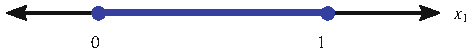
\includegraphics[width=0.561\linewidth]{images/vector/fig-11-1.pdf}
  \caption{画在 $x_1$-轴上的一维单位立方体.}
  \label{fig:11-1}
\end{figure}

\begin{figure}[htbp]
  \centering
  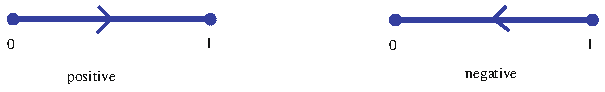
\includegraphics[width=0.728\linewidth]{images/vector/fig-11-2.pdf}
  \caption{一维单位立方体的两种定向. 定向由一维体积形式 $dx_1$ 决定，一般分别称为正定向（左）和负定向（右）.}
  \label{fig:11-2}
\end{figure}

\textbf{2 立方体 $I^2$}. 现在让我们考虑 2-立方体 $I^2=\{(x_1,x_2)\mid 0\leq x_i\leq 1,\ i=1,2\}$. 同样，体积形式 $dx_1\wedge dx_2$ 决定（我们常说诱导）$I^2$ 上的一个定向. 考虑两个单位向量
\[
e_1=\binom{1}{0},\qquad e_2=\binom{0}{1}.
\]
2-立方体正是由这两个单位向量张成的平行六面体，如图~\ref{fig:11-3} 所示. 利用二维体积形式 $dx_1\wedge dx_2$，我们有
\begin{align*}
dx_1\wedge dx_2\left(\binom{1}{0},\binom{0}{1}\right)=\begin{vmatrix}1&0\\0&1\end{vmatrix}=1>0, \\
dx_1\wedge dx_2\left(\binom{0}{1},\binom{1}{0}\right)=\begin{vmatrix}0&1\\1&0\end{vmatrix}=-1<0.
\end{align*}
因此，单位向量的次序决定了 2-立方体的定向. 次序
\[
\left\{\binom{1}{0},\binom{0}{1}\right\}
\]
表示正定向，而次序
\[
\left\{\binom{0}{1},\binom{1}{0}\right\}
\]
表示负定向. 正定向通常如图~\ref{fig:11-4} 所示用图形表示，而负定向通常如图~\ref{fig:11-5} 所示用图形表示.

\begin{figure}[htbp]
  \centering
  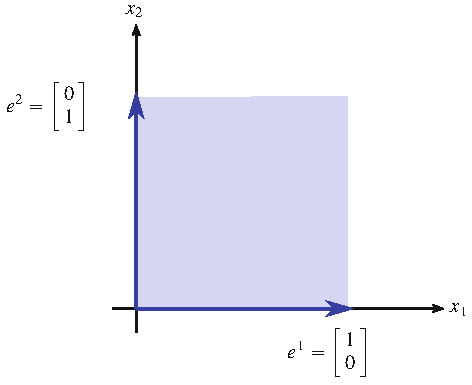
\includegraphics[width=0.559\linewidth]{images/vector/fig-11-3.pdf}
  \caption{二维单位立方体是由单位向量 $e_1$ 和 $e_2$ 张成的平行六面体.}
  \label{fig:11-3}
\end{figure}

\begin{figure}[htbp]
  \centering
  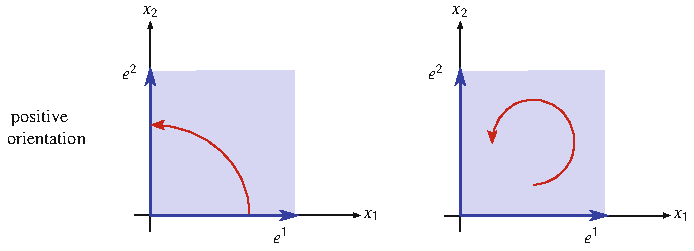
\includegraphics[width=0.822\linewidth]{images/vector/fig-11-4.pdf}
  \caption{利用体积形式 $dx_1\wedge dx_2$ 我们看到，次序 $\{e_1,e_2\}$，即先 $e_1$ 后 $e_2$，给出正定向. 图中展示了表示正定向的两种方式}
  \label{fig:11-4}
\end{figure}

\begin{figure}[htbp]
  \centering
  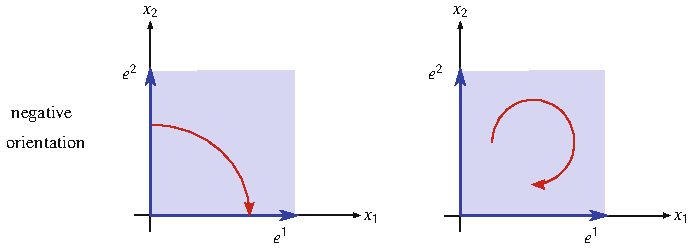
\includegraphics[width=0.822\linewidth]{images/vector/fig-11-5.pdf}
  \caption{利用体积形式 $dx_1\wedge dx_2$ 我们看到，次序 $\{e_2,e_1\}$，即先 $e_2$ 后 $e_1$，给出负定向. 图中展示了表示负定向的两种方式}
  \label{fig:11-5}
\end{figure}

\textbf{3 立方体 $I^3$}. 现在我们来看一看 3-立方体 $I^3=\{(x_1,x_2,x_3)\mid 0\leq x_i\leq 1,\ i=1,2,3\}$，如图~\ref{fig:11-6} 所示. 3-立方体正是由向量
\[
e_1=\begin{bmatrix}1\\0\\0\end{bmatrix},\qquad e_2=\begin{bmatrix}0\\1\\0\end{bmatrix},\qquad e_3=\begin{bmatrix}0\\0\\1\end{bmatrix}
\]
张成的平行六面体. 体积形式 $dx_1\wedge dx_2\wedge dx_3$ 决定（或诱导）$I^3$ 上的一个定向. 显然有
\[
dx_1\wedge dx_2\wedge dx_3\left(\begin{bmatrix}1\\0\\0\end{bmatrix},\begin{bmatrix}0\\1\\0\end{bmatrix},\begin{bmatrix}0\\0\\1\end{bmatrix}\right)=\begin{vmatrix}1&0&0\\0&1&0\\0&0&1\end{vmatrix}=1>0.
\]
因此，向量次序
\[
\left\{\begin{bmatrix}1\\0\\0\end{bmatrix},\begin{bmatrix}0\\1\\0\end{bmatrix},\begin{bmatrix}0\\0\\1\end{bmatrix}\right\}=\{e_1,e_2,e_3\}
\]
被认为是一个正定向. 正定向通常如图~\ref{fig:11-7} 所示用图形表示. 这正是所谓的"右手法则". 但注意，我们也有 $dx_1\wedge dx_2\wedge dx_3(e_2,e_3,e_1)=1$，所以 $\{e_2,e_3,e_1\}$ 也是一个正定向. 类似地，$dx_1\wedge dx_2\wedge dx_3(e_3,e_1,e_2)=1$，所以 $\{e_3,e_1,e_2\}$ 是又一个正定向. 于是我们看到，共有三种不同的次序给出 $I^3$ 的正定向. 接下来注意 $dx_1\wedge dx_2\wedge dx_3(e_2,e_1,e_3)=-1<0$，所以 $\{e_2,e_1,e_3\}$ 给出一个负定向，你可以把它看作"左手法则". 见图~\ref{fig:11-8}.

\begin{figure}[htbp]
  \centering
  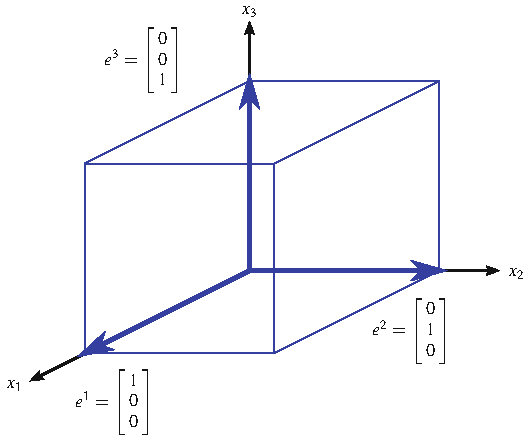
\includegraphics[width=0.628\linewidth]{images/vector/fig-11-6.pdf}
  \caption{三维单位立方体是由三个单位向量 $e_1$、$e_2$ 和 $e_3$ 张成的平行六面体}
  \label{fig:11-6}
\end{figure}

\begin{figure}[htbp]
  \centering
  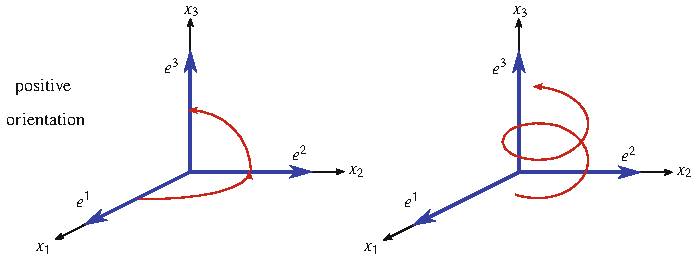
\includegraphics[width=0.827\linewidth]{images/vector/fig-11-7.pdf}
  \caption{利用体积形式 $dx_1\wedge dx_2\wedge dx_3$ 我们看到，次序 $\{e_1,e_2,e_3\}$，即先 $e_1$、再 $e_2$、再 $e_3$，给出正定向. 图中展示了表示正定向的两种方式. 三维中的正定向一般称为"右手法则"}
  \label{fig:11-7}
\end{figure}

\begin{figure}[htbp]
  \centering
  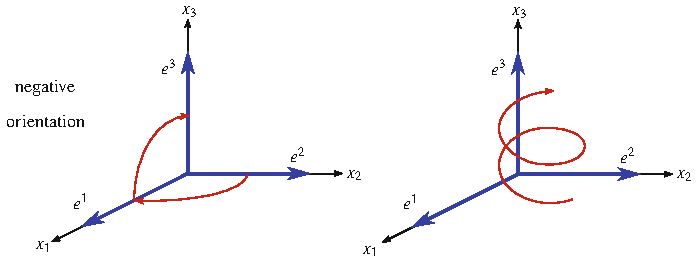
\includegraphics[width=0.827\linewidth]{images/vector/fig-11-8.pdf}
  \caption{利用体积形式 $dx_1\wedge dx_2\wedge dx_3$ 我们看到，次序 $\{e_2,e_1,e_3\}$，即先 $e_2$、再 $e_1$、再 $e_3$，给出负定向. 图中展示了表示负定向的两种方式. 三维中的负定向一般称为"左手法则"}
  \label{fig:11-8}
\end{figure}

\begin{question}\label{q:11-1}
给出 $I^3$ 负定向的三种次序是什么？
\end{question}

所以我们看到，给我们的基元素选取一个次序并不是标记或确定 $k$-立方体定向的一种很有效的方式. 这就是我们使用标准体积形式 $dx_1\wedge dx_2\wedge dx_3$——即下标按数值顺序排列的体积形式——的原因. 当然，这实际上归根结底还是为我们向量空间的基元素选取一个次序，但我们总得有个起点. 标准体积形式在每个单位立方体上诱导正定向和负定向，具体取决于我们如何排列用来生成立方体的单位向量.

\textbf{k 立方体 $I^k$}. 对于 $k>3$ 的 $I^k$，无论是 $k$-立方体还是其定向都无法画出，但思想是足够直观的. $k$-立方体是由单位向量 $e_1,e_2,\ldots,e_k$ 张成的平行六面体. 给定一个体积形式 $dx_1\wedge dx_2\wedge\cdots\wedge dx_k$，该体积形式就诱导一个定向. 例如，给定体积形式 $dx_1\wedge dx_2\wedge dx_3\wedge dx_4$，$e_1,e_2,e_3,e_4$ 的任何导致体积为正的次序都称为 $I^4$ 的正定向，任何导致体积为负的次序都称为负定向. 我们在图~\ref{fig:11-9} 中尝试"画出"$I^4$ 的一个正定向和一个负定向.

\begin{figure}[htbp]
  \centering
  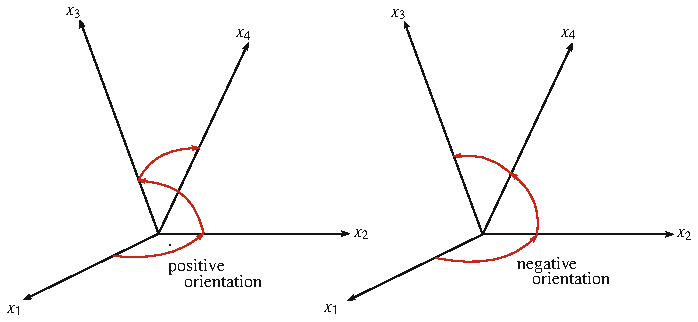
\includegraphics[width=0.827\linewidth]{images/vector/fig-11-9.pdf}
  \caption{为四维空间画出正定向（左）和负定向（右）的尝试. 由于有四个轴，它们不再能被画成彼此都与其他三个垂直，但应当理解为所画出的每个轴实际上都与其余三个垂直}
  \label{fig:11-9}
\end{figure}

\begin{question}\label{q:11-2}
求出 $e_1,e_2,e_3,e_4$ 的所有正定向和负定向.
\end{question}

\textbf{k-立方体的边界，$\partial I^k$}. 既然我们对单位立方体的定向有了一些概念，我们想要弄清楚单位立方体的边界是什么. 当然，你对边界是什么有一些直观的想法，但我们的目标是使这些想法在数学上精确. 我们还将考虑边界定向的思想，它起初可能有点令人困惑.

由于 0-立方体只是一个点，它没有边界. 我们起初并不考虑孤立点 $I^0$ 的定向，但在 $I^1$ 的边界这一背景下，我们将给一个点赋予定向. 首先我们将给出 $k$-立方体边界的一般定义，然后看一些边界的具体例子.

给定一个 $k$-立方体
\[
I^k=\left\{(x_1,\ldots,x_k)\,\bigl|\,0\leq x_i\leq 1,\ i=1,\ldots,k\right\},
\]
我们通过令 $x_i=0$ 来定义 $(i,0)$-面，于是有
\[
I^k_{(i,0)}=\left\{(x_1,\ldots,x_{i-1},0,x_{i+1},\ldots,x_k)\,\bigl|\,(x_1,\ldots,x_{i-1},0,x_{i+1},\ldots,x_k)\in I^k\right\},
\]
并通过令 $x_i=1$ 来定义 $(i,1)$-面，于是有
\[
I^k_{(i,1)}=\left\{(x_1,\ldots,x_{i-1},1,x_{i+1},\ldots,x_k)\,\bigl|\,(x_1,\ldots,x_{i-1},1,x_{i+1},\ldots,x_k)\in I^k\right\}.
\]
每个面 $I^k_{(i,a)}$（其中 $a=0,1$）将被赋予由 $(-1)^{i+a}$ 决定的定向. 若 $(-1)^{i+a}=1$，则定向为正；若 $(-1)^{i+a}=-1$，则定向为负. 我们将通过例子看出，为什么这是定义面的定向的恰当方式. $I^k$ 的边界记为 $\partial I^k$，它是 $I^k$ 的所有面连同所确定的定向的集合. 抽象地，我们写
\[
\partial I^k=\sum_{i=1}^{k}\sum_{a=0}^{1}(-1)^{i+a}I^k_{(i,a)},
\]
不过请记住，我们当然不是在通常意义下把这些面相加. 这仅仅是我们表示构成 $I^k$ 边界的各个面连同其各自定向的集合的方式.

\textbf{求 $\partial I^1$}. 让我们看看这对 $I^1$ 是如何进行的. 我们有
\[
I^1_{(1,0)}=\{(0)\},\qquad I^1_{(1,1)}=\{(1)\}.
\]
接下来我们看到，$I^1_{(1,0)}$ 具有负定向，因为 $(-1)^{1+0}=-1$；而 $I^1_{(1,1)}$ 具有正定向，因为 $(-1)^{1+1}=1$. 这在图~\ref{fig:11-10} 中作了说明. 最后，我们这样表示 $I^1$ 的边界：
\[
\partial I^1=\sum_{i=1}^{1}\sum_{a=0}^{1}(-1)^{i+a}I^1_{(i,a)}=I^1_{(1,1)}-I^1_{(1,0)}.
\]

\begin{figure}[htbp]
  \centering
  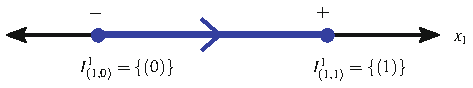
\includegraphics[width=0.561\linewidth]{images/vector/fig-11-10.pdf}
  \caption{带正定向的 1-立方体 $I^1$，连同带负定向的面 $I^1_{(1,0)}$ 和带正定向的面 $I^1_{(1,1)}$}
  \label{fig:11-10}
\end{figure}

\textbf{求 $\partial I^2$}. 接下来我们把注意力转向 $I^2$. 2-立方体有四个面，由下式给出：
\begin{align*}
I^2_{(1,0)}=\{(0,x_2)\mid(0,x_2)\in I^2\},\qquad
I^2_{(1,1)}=\{(1,x_2)\mid(1,x_2)\in I^2\}, \\
I^2_{(2,0)}=\{(x_1,0)\mid(x_1,0)\in I^2\},\qquad
I^2_{(2,1)}=\{(x_1,1)\mid(x_1,1)\in I^2\}.
\end{align*}
带边界的 2-立方体的图画如图~\ref{fig:11-11} 所示. 我们现在给 2-立方体的面赋予如下定向：
\begin{align*}
I^2_{(1,0)}\ \text{的定向由 }(-1)^{1+0}=-1\ \text{决定}\Rightarrow\text{负}, \\
I^2_{(1,1)}\ \text{的定向由 }(-1)^{1+1}=1\ \text{决定}\Rightarrow\text{正}, \\
I^2_{(2,0)}\ \text{的定向由 }(-1)^{2+0}=1\ \text{决定}\Rightarrow\text{正}, \\
I^2_{(2,1)}\ \text{的定向由 }(-1)^{2+1}=-1\ \text{决定}\Rightarrow\text{负},
\end{align*}
于是我们得到带定向边界的 2-立方体的图画，如图~\ref{fig:11-12} 所示. 注意，通过给面 $I^2_{(i,a)}$ 赋予由 $(-1)^{i+a}$ 决定的定向，我们的边界定向在某种意义上是自洽的，它们以一致的方式"绕"2-立方体一周. 我们这样表示 2-立方体的边界：
\[
\partial I^2=\sum_{i=1}^{2}\sum_{a=0}^{1}(-1)^{i+a}I^2_{(i,a)}=-I^2_{(1,0)}+I^2_{(1,1)}+I^2_{(2,0)}-I^2_{(2,1)}.
\]

\begin{figure}[htbp]
  \centering
  \includegraphics[width=0.549\linewidth]{images/vector/fig-11-11.pdf}
  \caption{2-立方体 $I^2$ 连同其边界，边界由四个面 $I^2_{(1,0)}$、$I^2_{(1,1)}$、$I^2_{(2,0)}$ 和 $I^2_{(2,1)}$ 给出. 四个面都以正定向显示}
  \label{fig:11-11}
\end{figure}

\begin{figure}[htbp]
  \centering
  \includegraphics[width=0.549\linewidth]{images/vector/fig-11-12.pdf}
  \caption{2-立方体 $I^2$ 连同其四个边界面，此处以由公式确定的定向显示. 例如，面 $I^2_{(i,a)}$ 的定向由 $(-1)^{i+a}$ 是正还是负来决定}
  \label{fig:11-12}
\end{figure}

\begin{question}\label{q:11-3}
图~\ref{fig:11-11} 中的 2-立方体是这样画的：四个边界都用箭头显示为正定向. 解释为什么箭头是它们所示的方向.
\end{question}

\textbf{求 $\partial\partial I^1$}. 退后一步，我们可以看出 $\partial\partial I^1=0$ 也成立. 我们已有 $\partial I^1=\{(1)\}-\{(0)\}$，其中 $(0)$ 和 $(1)$ 是 $\mathbb{R}^1$ 上的点. 由于点没有边界，我们说 $\partial\{(0)\}=0$，$\partial\{(1)\}=0$，于是得到
\[
\partial\partial I^1=\partial\{(1)\}-\partial\{(0)\}=0-0=0.
\]

\textbf{求 $\partial\partial I^2$}. 现在，我们将更进一步，求出边界元素的边界. 也就是说，我们将求 $\partial\bigl(-I^2_{(1,0)}\bigr)$、$\partial I^2_{(1,1)}$、$\partial I^2_{(2,0)}$ 和 $\partial\bigl(-I^2_{(2,1)}\bigr)$. 我们从 $\partial I^2_{(2,0)}$ 开始. 我们看到
\begin{align*}
\bigl(I^2_{(2,0)}\bigr)^1_{(1,0)}=\{(0,0)\}\quad\text{具有定向 }(-1)^{1+0}=-1\Rightarrow\text{负}, \\
\bigl(I^2_{(2,0)}\bigr)^1_{(1,1)}=\{(1,0)\}\quad\text{具有定向 }(-1)^{1+1}=1\Rightarrow\text{正}.
\end{align*}
我们在图~\ref{fig:11-13} 中展示了 $\partial I^2_{(2,0)}$.

\begin{figure}[htbp]
  \centering
  \includegraphics[width=0.720\linewidth]{images/vector/fig-11-13.pdf}
  \caption{$I^2_{(2,0)}$ 的边界由带负定向的 $\bigl(I^2_{(2,0)}\bigr)^1_{(1,0)}$ 和带正定向的 $\bigl(I^2_{(2,0)}\bigr)^1_{(1,1)}$ 给出}
  \label{fig:11-13}
\end{figure}

为了求 $\partial I^2_{(1,1)}$，我们需要特别注意下标. 回顾
\[
I^2_{(1,1)}=\left\{\bigl(1,x_2\bigr)\,\bigl|\,\bigl(1,x_2\bigr)\in I^2\right\}.
\]
注意，$I^2_{(1,1)}$ 现在实际上是一个 1-立方体，即 $I^2_{(1,1)}\simeq I^1$. 所以当我们想取这个 1-立方体的 $(1,0)$ 边界时，这个 1 所指的变量是这个 1-立方体中的第一个变量，而它实际上仍被标记为 $x_2$，
\[
\partial\bigl(I^2_{(1,1)}\bigr)^1_{(1,0)}=\{(1,0)\}.
\]
类似地，
\[
\partial\bigl(I^2_{(1,1)}\bigr)^1_{(1,1)}=\{(1,1)\}.
\]
至于定向，
\begin{align*}
\bigl(I^2_{(1,1)}\bigr)^1_{(1,0)}=\{(1,0)\}\quad\text{具有定向 }(-1)^{1+0}=-1\Rightarrow\text{负}, \\
\bigl(I^2_{(1,1)}\bigr)^1_{(1,1)}=\{(1,1)\}\quad\text{具有定向 }(-1)^{1+1}=1\Rightarrow\text{正}.
\end{align*}
然后我们可以像图~\ref{fig:11-14} 那样画出 $\partial I^2_{(1,1)}$.

\begin{figure}[htbp]
  \centering
  \includegraphics[width=0.402\linewidth]{images/vector/fig-11-14.pdf}
  \caption{$I^2_{(1,1)}$ 的边界由带负定向的 $\bigl(I^2_{(1,1)}\bigr)^1_{(1,0)}$ 和带正定向的 $\bigl(I^2_{(1,1)}\bigr)^1_{(1,1)}$ 给出}
  \label{fig:11-14}
\end{figure}

现在对于 $\partial\bigl(-I^2_{(2,1)}\bigr)$，我们看到
\begin{align*}
\bigl(-I^2_{(2,1)}\bigr)^1_{(1,0)}=\{(0,1)\}\quad\text{具有定向 }-(-1)^{1+0}=1\Rightarrow\text{正}, \\
\bigl(-I^2_{(2,1)}\bigr)^1_{(1,1)}=\{(1,1)\}\quad\text{具有定向 }-(-1)^{1+1}=-1\Rightarrow\text{负},
\end{align*}
从而允许我们像图~\ref{fig:11-15} 那样画出 $\partial\bigl(-I^2_{(2,1)}\bigr)$.

\begin{figure}[htbp]
  \centering
  \includegraphics[width=0.729\linewidth]{images/vector/fig-11-15.pdf}
  \caption{$-I^2_{(2,1)}$ 的边界由带正定向的 $\bigl(-I^2_{(2,1)}\bigr)^1_{(1,0)}$ 和带负定向的 $\bigl(-I^2_{(2,1)}\bigr)^1_{(1,1)}$ 给出}
  \label{fig:11-15}
\end{figure}

最后，对于 $\partial\bigl(-I^2_{(1,0)}\bigr)$，我们看到
\begin{align*}
\bigl(-I^2_{(1,0)}\bigr)^1_{(1,0)}=\{(0,0)\}\quad\text{具有定向 }-(-1)^{1+0}=1\Rightarrow\text{正}, \\
\bigl(-I^2_{(1,0)}\bigr)^1_{(1,1)}=\{(0,1)\}\quad\text{具有定向 }-(-1)^{1+1}=-1\Rightarrow\text{负},
\end{align*}
从而允许我们像图~\ref{fig:11-16} 那样画出 $\partial\bigl(-I^2_{(1,0)}\bigr)$.

\begin{figure}[htbp]
  \centering
  \includegraphics[width=0.534\linewidth]{images/vector/fig-11-16.pdf}
  \caption{$-I^2_{(1,0)}$ 的边界由带正定向的 $\bigl(-I^2_{(1,0)}\bigr)^1_{(1,0)}$ 和带负定向的 $\bigl(-I^2_{(1,0)}\bigr)^1_{(1,1)}$ 给出}
  \label{fig:11-16}
\end{figure}

把所有结果放在一起，对于 $\partial\partial I^2$，我们有图~\ref{fig:11-17} 中的图画，它给出
\[
\begin{aligned}
\partial\partial I^2&=\partial\bigl(-I^2_{(1,0)}\bigr)+\partial I^2_{(1,1)}+\partial I^2_{(2,0)}+\partial\bigl(-I^2_{(2,1)}\bigr)\\
&=\{(0,0)\}-\{(0,1)\}-\{(1,0)\}+\{(1,1)\}-\{(0,0)\}+\{(1,0)\}+\{(0,1)\}-\{(1,1)\}\\
&=0.
\end{aligned}
\]
于是我们看到，边界元素及其定向的定义方式使得边界的边界为零，这在直觉上说得通. 毕竟，闭曲线没有边界，而 2-立方体的边界正是一条闭曲线.

\begin{figure}[htbp]
  \centering
  \includegraphics[width=0.742\linewidth]{images/vector/fig-11-17.pdf}
  \caption{为了得到 $\partial\partial I^2$ 的图画，我们把图~\ref{fig:11-13}、\ref{fig:11-14}、\ref{fig:11-15} 和 \ref{fig:11-16} 拼在一起}
  \label{fig:11-17}
\end{figure}

\textbf{求 $\partial I^3$}. 现在我们将考虑 $I^3$. 首先求 $I^3$ 的面，然后求这些面的定向，我们将用它们来求 $\partial I^3$. $I^3$ 显然有六个面，由下式给出：
\begin{align*}
I^3_{(1,0)}=\{(0,x_2,x_3)\mid 0\leq x_2,x_3\leq 1\}=\text{后面}, \\
I^3_{(1,1)}=\{(1,x_2,x_3)\mid 0\leq x_2,x_3\leq 1\}=\text{前面}, \\
I^3_{(2,0)}=\{(x_1,0,x_3)\mid 0\leq x_1,x_3\leq 1\}=\text{左面}, \\
I^3_{(2,1)}=\{(x_1,1,x_3)\mid 0\leq x_1,x_3\leq 1\}=\text{右面}, \\
I^3_{(3,0)}=\{(x_1,x_2,0)\mid 0\leq x_1,x_2\leq 1\}=\text{底面}, \\
I^3_{(3,1)}=\{(x_1,x_2,1)\mid 0\leq x_1,x_2\leq 1\}=\text{顶面},
\end{align*}
并在图~\ref{fig:11-18} 中作了展示.

\begin{figure}[htbp]
  \centering
  \includegraphics[width=0.859\linewidth]{images/vector/fig-11-18.pdf}
  \caption{3-立方体 $I^3$ 连同其六个面}
  \label{fig:11-18}
\end{figure}

我们首先展示 $I^3$ 全部六个面的正定向. 决定前面和后面定向的体积形式是 $dx_2\wedge dx_3$，因为前面和后面位于 $(x_2,x_3)$-平面中. 考虑两个向量
\[
\begin{bmatrix}0\\1\\0\end{bmatrix},\qquad\begin{bmatrix}0\\0\\1\end{bmatrix}
\]
在后面的点 $p=(0,0,0)$ 处和前面的点 $q=(1,0,0)$ 处. 对这两个点，我们都有
\begin{align*}
dx_2\wedge dx_3(p)\left(\begin{bmatrix}0\\1\\0\end{bmatrix}_{\!p},\begin{bmatrix}0\\0\\1\end{bmatrix}_{\!p}\right)=\begin{vmatrix}1&0\\0&1\end{vmatrix}=1, \\
dx_2\wedge dx_3(q)\left(\begin{bmatrix}0\\1\\0\end{bmatrix}_{\!q},\begin{bmatrix}0\\0\\1\end{bmatrix}_{\!q}\right)=\begin{vmatrix}1&0\\0&1\end{vmatrix}=1.
\end{align*}
前面和后面的正定向如图~\ref{fig:11-19} 所示.

\begin{figure}[htbp]
  \centering
  \includegraphics[width=0.748\linewidth]{images/vector/fig-11-19.pdf}
  \caption{带正定向显示的 $I^3$ 的前面和后面}
  \label{fig:11-19}
\end{figure}

决定左面和右面正定向的体积形式是 $dx_1\wedge dx_3$，因为左面和右面位于 $(x_1,x_3)$-平面中. 与前面完全一样，考虑两个向量
\[
\begin{bmatrix}1\\0\\0\end{bmatrix},\qquad\begin{bmatrix}0\\0\\1\end{bmatrix}
\]
在左面的点 $p=(0,0,0)$ 处和右面的点 $q=(0,1,0)$ 处. 对这两个点，我们都有
\begin{align*}
dx_1\wedge dx_3(p)\left(\begin{bmatrix}1\\0\\0\end{bmatrix}_{\!p},\begin{bmatrix}0\\0\\1\end{bmatrix}_{\!p}\right)=\begin{vmatrix}1&0\\0&1\end{vmatrix}=1, \\
dx_1\wedge dx_3(q)\left(\begin{bmatrix}1\\0\\0\end{bmatrix}_{\!q},\begin{bmatrix}0\\0\\1\end{bmatrix}_{\!q}\right)=\begin{vmatrix}1&0\\0&1\end{vmatrix}=1.
\end{align*}
左面和右面的正定向如图~\ref{fig:11-20} 所示.

\begin{figure}[htbp]
  \centering
  \includegraphics[width=0.724\linewidth]{images/vector/fig-11-20.pdf}
  \caption{带正定向显示的 $I^3$ 的左面和右面}
  \label{fig:11-20}
\end{figure}

\begin{question}\label{q:11-4}
对顶面和底面做同样的分析，以得到图~\ref{fig:11-21} 所示的这两个面的正定向.
\end{question}

\begin{figure}[htbp]
  \centering
  \includegraphics[width=0.703\linewidth]{images/vector/fig-11-21.pdf}
  \caption{带正定向显示的 $I^3$ 的顶面和底面}
  \label{fig:11-21}
\end{figure}

现在我们算出六个面的定向.
\begin{align*}
I^3_{(1,0)}\ \text{的定向由 }(-1)^{1+0}=-1\ \text{决定}\Rightarrow\text{负}, \\
I^3_{(1,1)}\ \text{的定向由 }(-1)^{1+1}=+1\ \text{决定}\Rightarrow\text{正}, \\
I^3_{(2,0)}\ \text{的定向由 }(-1)^{2+0}=+1\ \text{决定}\Rightarrow\text{正}, \\
I^3_{(2,1)}\ \text{的定向由 }(-1)^{2+1}=-1\ \text{决定}\Rightarrow\text{负}, \\
I^3_{(3,0)}\ \text{的定向由 }(-1)^{3+0}=-1\ \text{决定}\Rightarrow\text{负}, \\
I^3_{(3,1)}\ \text{的定向由 }(-1)^{3+1}=+1\ \text{决定}\Rightarrow\text{正}.
\end{align*}
把所有结果放在一起，我们可以写出 $I^3$ 的边界：
\[
\partial I^3=\sum_{i=1}^{3}\sum_{a=0}^{1}(-1)^{i+a}I^3_{(i,a)}
=-I^3_{(1,0)}+I^3_{(1,1)}+I^3_{(2,0)}-I^3_{(2,1)}-I^3_{(3,0)}+I^3_{(3,1)}.
\]

\begin{question}\label{q:11-5}
画出单位立方体 $I^3$ 的草图，包括各个面的适当定向. 这些定向看起来是否彼此吻合？
\end{question}

\textbf{求 $\partial\partial I^3$}. 现在我们想求 $\partial I^3$ 的边界. 回顾，$\partial I^3$ 由六个不同的 2-立方体组成. 我们将从求底面 $I^3_{(3,0)}$ 的边开始：
\begin{align*}
\bigl(I^3_{(3,0)}\bigr)^2_{(1,0)}=\{(0,x_2,0)\mid 0\leq x_2\leq 1\}\quad\text{具有定向 }(-1)^{3+0}(-1)^{1+0}=1, \\
\bigl(I^3_{(3,0)}\bigr)^2_{(1,1)}=\{(1,x_2,0)\mid 0\leq x_2\leq 1\}\quad\text{具有定向 }(-1)^{3+0}(-1)^{1+1}=-1, \\
\bigl(I^3_{(3,0)}\bigr)^2_{(2,0)}=\{(x_1,0,0)\mid 0\leq x_1\leq 1\}\quad\text{具有定向 }(-1)^{3+0}(-1)^{2+0}=-1, \\
\bigl(I^3_{(3,0)}\bigr)^2_{(2,1)}=\{(x_1,1,0)\mid 0\leq x_1\leq 1\}\quad\text{具有定向 }(-1)^{3+0}(-1)^{2+1}=1.
\end{align*}
类似地，顶面 $I^3_{(3,1)}$ 的边为
\begin{align*}
\bigl(I^3_{(3,1)}\bigr)^2_{(1,0)}=\{(0,x_2,1)\mid 0\leq x_2\leq 1\}\quad\text{具有定向 }(-1)^{3+1}(-1)^{1+0}=-1, \\
\bigl(I^3_{(3,1)}\bigr)^2_{(1,1)}=\{(1,x_2,1)\mid 0\leq x_2\leq 1\}\quad\text{具有定向 }(-1)^{3+1}(-1)^{1+1}=1, \\
\bigl(I^3_{(3,1)}\bigr)^2_{(2,0)}=\{(x_1,0,1)\mid 0\leq x_1\leq 1\}\quad\text{具有定向 }(-1)^{3+1}(-1)^{2+0}=1, \\
\bigl(I^3_{(3,1)}\bigr)^2_{(2,1)}=\{(x_1,1,1)\mid 0\leq x_1\leq 1\}\quad\text{具有定向 }(-1)^{3+1}(-1)^{2+1}=-1.
\end{align*}
我们在图~\ref{fig:11-22} 中展示了 $I^3$ 的底面和顶面连同其边界边的定向.

\begin{figure}[htbp]
  \centering
  \includegraphics[width=0.650\linewidth]{images/vector/fig-11-22.pdf}
  \caption{3-立方体的底面和顶面，连同其边界的定向}
  \label{fig:11-22}
\end{figure}

确保你理解上面的记号是如何工作的. 底面/顶面的情形是最简单的情形. 对于后面/前面和左面/右面，记号中有一些有点棘手的地方. 让我们首先考虑后面 $I^3_{(1,0)}=\{(0,x_2,x_3)\mid 0\leq x_2,x_3\leq 1\}$，它是一个 2-立方体. 让我们首先考虑 $\bigl(I^3_{(1,0)}\bigr)^2_{(1,0)}$. 对于 3-立方体，变量是 $(x_1,x_2,x_3)$. $I^3_{(1,0)}$ 中的 $(1,0)$ 表示第一个变量 $x_1$ 被替换为 $0$. 但现在让我们考虑 3-立方体的后面，它是一个 2-立方体，即 $\bigl(I^3_{(1,0)}\bigr)^2_{(1,0)}$. 对于这个 2-立方体，变量是 $(x_2,x_3)$，所以 $\bigl(I^3_{(1,0)}\bigr)^2_{(1,0)}$ 中第二个 $(1,0)$ 表示第一个变量被替换为 $0$，但在这种情况下第一个变量是 $x_2$. 于是我们有
\[
\bigl(I^3_{(1,0)}\bigr)^2_{(1,0)}=\{(0,0,x_3)\mid 0\leq x_3\leq 1\}.
\]
其定向为 $(-1)^{1+0}(-1)^{1+0}=1$，是正的. 类似地，我们有
\begin{align*}
\bigl(I^3_{(1,0)}\bigr)^2_{(1,1)}=\{(0,1,x_3)\mid 0\leq x_3\leq 1\}\quad\text{具有定向 }(-1)^{1+0}(-1)^{1+1}=-1\Rightarrow\text{负}, \\
\bigl(I^3_{(1,0)}\bigr)^2_{(2,0)}=\{(0,x_2,0)\mid 0\leq x_2\leq 1\}\quad\text{具有定向 }(-1)^{1+0}(-1)^{2+0}=-1\Rightarrow\text{负}, \\
\bigl(I^3_{(1,0)}\bigr)^2_{(2,1)}=\{(0,x_2,1)\mid 0\leq x_2\leq 1\}\quad\text{具有定向 }(-1)^{1+0}(-1)^{2+1}=1\Rightarrow\text{正}.
\end{align*}
3-立方体的后面连同边界定向如图~\ref{fig:11-23} 所示.

\begin{figure}[htbp]
  \centering
  \includegraphics[width=0.960\linewidth]{images/vector/fig-11-23.pdf}
  \caption{3-立方体 $I^3$ 的前面和后面，连同其边界的定向}
  \label{fig:11-23}
\end{figure}

\begin{question}\label{q:11-6}
求前面 $I^3_{(1,1)}=\{(1,x_2,x_3)\mid 0\leq x_2,x_3\leq 1\}$ 的四条边界边，并求这些边的定向. 你的答案应与图~\ref{fig:11-23} 一致.
\end{question}

\begin{question}\label{q:11-7}
证明：当考虑定向时，$\bigl(I^3_{(3,1)}\bigr)^2_{(1,0)}=-\bigl(I^3_{(1,0)}\bigr)^2_{(2,1)}$，且 $\bigl(I^3_{(3,0)}\bigr)^2_{(1,0)}=-\bigl(I^3_{(1,0)}\bigr)^2_{(2,0)}$. 见图~\ref{fig:11-24}.
\end{question}

\begin{figure}[htbp]
  \centering
  \includegraphics[width=0.715\linewidth]{images/vector/fig-11-24.pdf}
  \caption{3-立方体 $I^3$ 的顶面、底面和后面，连同其边界. 注意三个面的边界在何处相同：当考虑定向时，我们有 $\bigl(I^3_{(3,1)}\bigr)^2_{(1,0)}=-\bigl(I^3_{(1,0)}\bigr)^2_{(2,1)}$，且 $\bigl(I^3_{(3,0)}\bigr)^2_{(1,0)}=-\bigl(I^3_{(1,0)}\bigr)^2_{(2,0)}$}
  \label{fig:11-24}
\end{figure}

\begin{question}\label{q:11-8}
证明：当考虑定向时，$\bigl(I^3_{(3,1)}\bigr)^2_{(1,1)}=-\bigl(I^3_{(1,1)}\bigr)^2_{(2,1)}$，且 $\bigl(I^3_{(3,0)}\bigr)^2_{(1,1)}=-\bigl(I^3_{(1,1)}\bigr)^2_{(2,0)}$. 见图~\ref{fig:11-25}.
\end{question}

\begin{figure}[htbp]
  \centering
  \includegraphics[width=0.719\linewidth]{images/vector/fig-11-25.pdf}
  \caption{3-立方体 $I^3$ 的顶面、底面和前面，连同其边界. 注意三个面的边界在何处相同：当考虑定向时，我们有 $\bigl(I^3_{(3,1)}\bigr)^2_{(1,1)}=-\bigl(I^3_{(1,1)}\bigr)^2_{(2,1)}$，且 $\bigl(I^3_{(3,0)}\bigr)^2_{(1,1)}=-\bigl(I^3_{(1,1)}\bigr)^2_{(2,0)}$}
  \label{fig:11-25}
\end{figure}

\begin{question}\label{q:11-9}
求左面 $I^3_{(2,0)}=\{(x_1,0,x_3)\mid 0\leq x_1,x_3\leq 1\}$ 和右面 $I^3_{(2,1)}=\{(x_1,1,x_3)\mid 0\leq x_1,x_3\leq 1\}$ 的四条边界边，并求这八条边界边的定向. 把顶面、左面和底面画在一起，然后再把顶面、右面和底面画在一起.
\end{question}

通过检查各种草图，你应该能够看出，下列 1-立方体是等同的：
\begin{align*}
\bigl(I^3_{(2,0)}\bigr)^2_{(1,0)}=\bigl(I^3_{(1,0)}\bigr)^2_{(1,0)}, \\
\bigl(I^3_{(2,1)}\bigr)^2_{(1,1)}=\bigl(I^3_{(1,1)}\bigr)^2_{(1,0)}, \\
\bigl(I^3_{(2,0)}\bigr)^2_{(2,0)}=\bigl(I^3_{(3,0)}\bigr)^2_{(2,0)}, \\
\bigl(I^3_{(2,0)}\bigr)^2_{(2,1)}=\bigl(I^3_{(3,1)}\bigr)^2_{(2,0)}.
\end{align*}

\begin{question}\label{q:11-10}
把所有结果放在一起，证明 $\partial\partial I^3=0$.
\end{question}

\textbf{求 $\partial\partial I^k$}. 考虑 $i\leq j\leq k-1$ 且 $a,b=0,1$ 的情形：
\[
\begin{aligned}
\bigl(I^k_{(i,a)}\bigr)^{k-1}_{(j,b)}&=\bigl\{(x_1,\ldots,x_{i-1},a,x_{i+1},\ldots,x_k)\bigr\}^{k-1}_{(j,b)}\\
&=\bigl\{(x_1,\ldots,x_{i-1},a,x_i,\ldots,x_{k-1})\bigr\}^{k-1}_{(j,b)}\quad(\text{重新标记为 }(k-1)\text{-立方体的变量名})\\
&=\bigl\{(x_1,\ldots,x_{i-1},a,x_i,\ldots,x_{j-1},b,x_{j+1},\ldots,x_{k-1})\bigr\}\\
&=\bigl\{(x_1,\ldots,x_{i-1},a,x_{i+1},\ldots,x_j,b,x_{j+2},\ldots,x_k)\bigr\}\\
&\qquad(\text{重新标记为 }k\text{-立方体的变量名}),
\end{aligned}
\]
所以当我们使用 $k$-立方体的变量名时，$b$ 位于第 $j+1$ 个位置. 我们还有
\[
\begin{aligned}
\bigl(I^k_{(j+1,b)}\bigr)^{k-1}_{(i,a)}&=\bigl\{(x_1,\ldots,x_j,b,x_{j+2},\ldots,x_k)\bigr\}^{k-1}_{(i,a)}\\
&=\bigl\{(x_1,\ldots,x_{i-1},a,x_{i+1},\ldots,x_j,b,x_{j+2},\ldots,x_k)\bigr\}\\
&\qquad(\text{由于 }i\leq j\text{，无需重新标记}).
\end{aligned}
\]
因此，对 $i\leq j\leq k-1$，我们有
\[
\bigl(I^k_{(i,a)}\bigr)^{k-1}_{(j,b)}=\bigl(I^k_{(j+1,b)}\bigr)^{k-1}_{(i,a)}.
\]

\begin{question}\label{q:11-11}
解释为什么条件 $i\leq j\leq k-1$ 并不构成限制. 也就是说，$\partial I^k$ 的每个边界元素都被包括了.
\end{question}

\begin{question}\label{q:11-12}
证明对一般的 $I^k$，有 $\partial\partial I^k=0$.
\end{question}

\section{基础情形：$I^k$ 上的 Stokes 定理}

在覆盖了所有这些必要的背景材料之后，Stokes 定理的实际证明其实并不那么困难. 正如我们前面所说，我们将以"自举"的方式一路推进到完全一般的情形. 第一步是在 $k$-立方体 $I^k$ 上证明 Stokes 定理. 给定定义在单位 $k$-立方体 $I^k$ 的某个邻域上的 $(k-1)$-形式 $\alpha$，我们想证明
\[
\int_{I^k}d\alpha=\int_{\partial I^k}\alpha.
\]

首先，$\alpha$ 是定义在 $I^k\subset\mathbb{R}^k$ 的某个邻域上的 $(k-1)$-形式，所以 $\alpha$ 具有一般形式
\[
\begin{aligned}
\alpha&=\alpha_1(x_1,\ldots,x_k)\,dx_2\wedge dx_3\wedge\cdots\wedge dx_k\\
&\quad+\alpha_2(x_1,\ldots,x_k)\,dx_1\wedge dx_3\wedge\cdots\wedge dx_k\\
&\quad+\cdots\\
&\quad+\alpha_k(x_1,\ldots,x_k)\,dx_1\wedge dx_2\wedge\cdots\wedge dx_{k-1}\\
&=\sum_{i=1}^{k}\alpha_i(x_1,\ldots,x_k)\,dx_1\wedge\cdots\wedge\widehat{dx_i}\wedge\cdots\wedge dx_k,
\end{aligned}
\]
其中 $\widehat{dx_i}$ 表示 $dx_i$ 被省略，$\alpha_i:\mathbb{R}^k\to\mathbb{R}$（$1\leq i\leq k$）是定义在 $I^k$ 的某个邻域上的实值函数. 我们知道外微分 $d$ 是线性的，这意味着
\[
d\left(\sum_{i=1}^{k}\alpha_i\,dx_1\wedge\cdots\wedge\widehat{dx_i}\wedge\cdots\wedge dx_k\right)=\sum_{i=1}^{k}d\left(\alpha_i\,dx_1\wedge\cdots\wedge\widehat{dx_i}\wedge\cdots\wedge dx_k\right).
\]
我们还知道积分是线性的，所以
\[
\int_{I^k}\sum_{i=1}^{k}d\left(\alpha_i\,dx_1\wedge\cdots\wedge\widehat{dx_i}\wedge\cdots\wedge dx_k\right)=\sum_{i=1}^{k}\int_{I^k}d\left(\alpha_i\,dx_1\wedge\cdots\wedge\widehat{dx_i}\wedge\cdots\wedge dx_k\right).
\]

现在让我们考虑 $(k-1)$-形式 $\alpha$ 的第一项，即 $\alpha_1\,dx_2\wedge\cdots\wedge dx_k$. 于是我们有
\[
\begin{aligned}
\int_{I^k}d\bigl(\alpha_1\,dx_2\wedge\cdots\wedge dx_k\bigr)
&=\int_{I^k}\frac{\partial\alpha_1}{\partial x_1}\,dx_1\wedge dx_2\wedge\cdots\wedge dx_k\\
&=\int_{x_k=0}^{1}\cdots\int_{x_2=0}^{1}\int_{x_1=0}^{1}\frac{\partial\alpha_1}{\partial x_1}\,dx_1dx_2\cdots dx_k\\
&\quad(\text{传统积分（定向无关紧要）})\\
&=\int_{x_k=0}^{1}\cdots\int_{x_2=0}^{1}\Bigl[\alpha_1(x_1,x_2,\ldots,x_k)\Bigr]_{0}^{1}\,dx_2\cdots dx_k\\
&\quad(\text{微积分基本定理})\\
&=\int_{x_k=0}^{1}\cdots\int_{x_2=0}^{1}\Bigl(\alpha_1(1,x_2,\ldots,x_k)\\
&\quad-\alpha_1(0,x_2,\ldots,x_k)\Bigr)\,dx_2\cdots dx_k\\
&=\int_{x_k=0}^{1}\cdots\int_{x_2=0}^{1}\alpha_1(1,x_2,\ldots,x_k)\\
&\quad\cdot dx_2\cdots dx_k\\
&\quad(\text{$\alpha_1$ 限制在面 }I^k_{(1,1)}\text{ 上的积分})\\
&\quad-\int_{x_k=0}^{1}\cdots\int_{x_2=0}^{1}\alpha_1(0,x_2,\ldots,x_k)\\
&\quad\cdot dx_2\cdots dx_k\\
&\quad(\text{$\alpha_1$ 限制在面 }I^k_{(1,0)}\text{ 上的积分})\\
&=\int_{I^k_{(1,1)}}\alpha_1\,dx_2\wedge\cdots\wedge dx_k\\
&\qquad-\int_{I^k_{(1,0)}}\alpha_1\,dx_2\wedge\cdots\wedge dx_k.
\end{aligned}
\]

正如你所注意到的，我们把记号从第二行中的 $dx_1\wedge dx_2\wedge\cdots\wedge dx_k$ 换成第三行中的 $dx_1dx_2\cdots dx_k$，然后再从传统记号换回最后一行中的 $dx_2\wedge\cdots\wedge dx_k$. 正如你大概还记得的（来自前面某章），你在微积分课上学到的传统积分与微分形式的积分只在一个方面有所不同：它不追踪曲面的定向. 我们做这种切换是为了使用微积分基本定理，而我们只知道基本定理的传统记号形式. 在使用传统记号的过程中，我们所做的一切都不会影响我们正在其上积分的立方体的定向. 我们之所以认识到这一点，是因为当我们从形式记号切换到传统记号、然后再从传统记号切换回形式记号时，次序是一致的. 要看到这一点，请比较第二行中的体积形式 $dx_1\wedge dx_2\wedge\cdots\wedge dx_k$ 与最后一行中的体积形式 $dx_2\wedge\cdots\wedge dx_k$. 最后一行中的体积形式比第一行中的低一维，它缺少 $dx_1$ 项，因为我们针对 $dx_1$ 项进行了积分；但除了这一处省略之外，其余 $k-1$ 项的次序没有改变. 因为当我们要换回形式记号时剩余项的次序没有改变，所以一切都是一致的. 为方便起见，我们将改写刚得到的这个等式，把 $\alpha$ 的第一项记为 $\alpha_1$ 而不是 $\alpha_1\,dx_2\wedge\cdots\wedge dx_k$，于是我们有
\[
\int_{I^k}d\alpha_1=\int_{I^k_{(1,1)}}\alpha_1-\int_{I^k_{(1,0)}}\alpha_1.
\]
这诚然是对记号的轻微滥用，但它确实大大简化了事情.

现在我们花一点时间来说明，$(k-1)$-形式 $\alpha_1\,dx_2\wedge\cdots\wedge dx_k$ 在 $\partial I^k$ 的所有其他面上的积分为零，并且我们在 $I^k$ 的边界上积分 $\alpha_1$ 时所预期得到的唯一贡献，正是上述等式右端所给出的那个贡献. $\partial I^k$ 的所有其他面都具有 $I^k_{(i,a)}$ 的形式，其中 $2\leq i\leq k$，$a=0,1$.

现在回顾 $dx_2\wedge dx_3\wedge\cdots\wedge dx_k$ 的作用：它把平行六面体投影到 $(x_2\cdots x_k)$-平面并求该投影的体积. 我们有兴趣在 $I^k$ 的各个面上取 $\alpha_1$ 的积分. 考虑 $I^k_{(1,1)}$，它是一个 $(k-1)$ 维平行六面体. 把 $I^k_{(1,1)}$ 投影到 $(x_2\cdots x_k)$-平面并求这个投影的体积，得到的体积为 1. 类似地，把 $I^k_{(1,0)}$ 投影到 $(x_2\cdots x_k)$-平面，得到的体积也为 1. 见图~\ref{fig:11-26}. 于是我们能够在这个面上取 $\alpha_1$ 的积分.

\begin{figure}[htbp]
  \centering
  \includegraphics[width=0.960\linewidth]{images/vector/fig-11-26.pdf}
  \caption{求 $I^k$ 的各面投影到 $(x_2\cdots x_k)$-平面时的体积}
  \label{fig:11-26}
\end{figure}

但现在考虑 $I^k_{(2,1)}$. 当把这个面投影到 $(x_2\cdots x_k)$-平面上时，其 $(k-1)$ 维体积为零，因为 $I^k_{(2,1)}$ 在 $(x_2\cdots x_k)$-平面上的投影是一个 $(k-2)$ 维集合，它具有零 $(k-1)$ 维体积. 因此 $\int_{I^k_{(2,1)}}\alpha_1=0$. 类似地，我们得出对所有 $j=2,\ldots,k$ 和 $a=0,1$，$\int_{I^k_{(j,a)}}\alpha_1=0$，见图~\ref{fig:11-26}. 于是，$I^k$ 的边界上唯一能给出非零贡献的积分，就是我们已有的 $\int_{I^k_{(1,1)}}\alpha_1$ 和 $\int_{I^k_{(1,0)}}\alpha_1$.

另外，注意我们所发现的：
\[
\int_{I^k}d\alpha_1=\int_{I^k_{(1,1)}}\alpha_1-\int_{I^k_{(1,0)}}\alpha_1.
\]
在 $I^k_{(1,1)}$ 上的积分是正的，这正与面 $I^k_{(1,1)}$ 在 $I^k$ 的边界中的定向一致，因为 $(-1)^{1+1}=1$. 类似地，在 $I^k_{(1,0)}$ 上的积分是负的，这正与面 $I^k_{(1,0)}$ 在 $I^k$ 的边界中的定向一致，因为 $(-1)^{1+0}=-1$. 于是我们可以——事实上也确实——作如下定义
\[
\int_{I^k_{(1,1)}}\alpha_1-\int_{I^k_{(1,0)}}\alpha_1\equiv\int_{I^k_{(1,1)}-I^k_{(1,0)}}\alpha_1,
\]
这允许我们写
\[
\int_{I^k}d\alpha_1=\int_{I^k_{(1,1)}-I^k_{(1,0)}}\alpha_1.
\]

现在我们将考察 $\alpha$ 的第二项. 我们有
\[
\begin{aligned}
\int_{I^k}d\bigl(\alpha_2\,dx_1\wedge dx_3\wedge\cdots\wedge dx_k\bigr)
&=\int_{I^k}\frac{\partial\alpha_2}{\partial x_2}\,dx_2\wedge dx_1\wedge dx_3\wedge\cdots\wedge dx_k\\
&=(-1)\int_{I^k}\frac{\partial\alpha_2}{\partial x_2}\,dx_1\wedge dx_2\wedge dx_3\wedge\cdots\wedge dx_k\\
&=(-1)\int_{x_k=0}^{1}\cdots\int_{x_2=0}^{1}\int_{x_1=0}^{1}\frac{\partial\alpha_2}{\partial x_2}\,dx_1dx_2\cdots dx_k\\
&\quad(\text{传统积分（定向无关紧要）})\\
&=(-1)\int_{x_k=0}^{1}\cdots\int_{x_1=0}^{1}\int_{x_2=0}^{1}\frac{\partial\alpha_2}{\partial x_2}\,dx_2dx_1\cdots dx_k\\
&\quad(\text{Fubini 定理})\\
&=(-1)\int_{x_k=0}^{1}\cdots\int_{x_1=0}^{1}\Bigl[\alpha_2(x_1,x_2,x_3,\ldots,x_k)\Bigr]_{0}^{1}\\
&\quad\cdot dx_1dx_3\cdots dx_k\\
&\quad(\text{微积分基本定理})\\
&=(-1)\int_{x_k=0}^{1}\cdots\int_{x_3=0}^{1}\int_{x_1=0}^{1}\\
&\quad\Bigl(\alpha_2(x_1,1,x_3,\ldots,x_k)\\
&\quad-\alpha_2(x_1,0,x_3,\ldots,x_k)\Bigr)\,dx_1dx_3\cdots dx_k\\
&=(-1)\int_{x_k=0}^{1}\cdots\int_{x_3=0}^{1}\int_{x_1=0}^{1}\alpha_2(x_1,1,x_3,\ldots,x_k)\\
&\quad\cdot dx_1dx_3\cdots dx_k\\
&\quad(\text{$\alpha_2$ 限制在面 }I^k_{(2,1)}\text{ 上的积分})\\
&\quad-(-1)\int_{x_k=0}^{1}\cdots\int_{x_3=0}^{1}\int_{x_1=0}^{1}\alpha_2(x_1,0,x_3,\ldots,x_k)\\
&\quad\cdot dx_1dx_3\cdots dx_k\\
&\quad(\text{$\alpha_2$ 限制在面 }I^k_{(2,0)}\text{ 上的积分})\\
&=-\int_{I^k_{(2,1)}}\alpha_2\,dx_1\wedge dx_3\wedge\cdots\wedge dx_k\\
&\quad+\int_{I^k_{(2,0)}}\alpha_2\,dx_1\wedge dx_3\wedge\cdots\wedge dx_k\\
&=\int_{-I^k_{(2,1)}+I^k_{(2,0)}}\alpha_2\\
&\quad\cdot dx_1\wedge dx_3\wedge\cdots\wedge dx_k.
\end{aligned}
\]

正如你所注意到的，我们把记号从第三行中的 $dx_1\wedge dx_2\wedge\cdots\wedge dx_k$ 换成第四行中的 $dx_1dx_2\cdots dx_k$，然后再换回倒数第二行中的 $dx_1\wedge dx_3\wedge\cdots\wedge dx_k$. 我们做这种切换是为了同时使用 Fubini 定理和微积分基本定理，而我们只知道这两个定理的传统记号形式. 你可能会想，在应用 Fubini 定理时交换积分次序会不会改变我们的体积-定向，但由于传统积分不追踪体积-定向的符号，这种改变不会改变相伴的体积-定向符号. 这意味着重要的是，当我们在传统记号与形式记号之间来回切换时，体积形式的定向是一致的. 例如，第三行中的体积形式是 $dx_1\wedge dx_2\wedge dx_3\wedge\cdots\wedge dx_k$，而倒数第二行中的体积形式是 $dx_1\wedge dx_3\wedge\cdots\wedge dx_k$. 虽然倒数第二行中缺少 $dx_2$（因为我们针对该项进行了积分），但剩余项的次序没有改变，因此是一致的.

注意这些符号再次与 $I^k$ 的边界中各面的定向相符. 这使我们能够改写这个计算的结果. 如果我们另外采用我们之前使用过的同样的记号滥用，把 $\alpha_2\,dx_1\wedge dx_3\wedge\cdots\wedge dx_k$ 写成 $\alpha_2$，我们就得到等式
\[
\int_{I^k}d\alpha_2=\int_{-I^k_{(2,1)}+I^k_{(2,0)}}\alpha_2.
\]

既然我们已经对 $(k-1)$-形式的头两项做了这个处理，你就对我们将要如何进行有了些概念. 现在我们将对整个
\[
\alpha=\sum_{i=1}^{k}\alpha_i\,dx_1\wedge\cdots\wedge\widehat{dx_i}\wedge\cdots\wedge dx_k
\]
做这个处理，其中 $\widehat{dx_i}$ 表示第 $i$ 项 $dx_i$ 被省略. 首先我们求 $d\alpha$，
\[
\begin{aligned}
d\left(\sum_{i=1}^{k}\alpha_i\,dx_1\wedge\cdots\wedge\widehat{dx_i}\wedge\cdots\wedge dx_k\right)
&=\sum_{i=1}^{k}d\left(\alpha_i\,dx_1\wedge\cdots\wedge\widehat{dx_i}\wedge\cdots\wedge dx_k\right)\\
&=\sum_{i=1}^{k}\frac{\partial\alpha_i}{\partial x_i}\,dx_i\wedge dx_1\wedge\cdots\wedge\widehat{dx_i}\wedge\cdots\wedge dx_k\\
&=\sum_{i=1}^{k}(-1)^{i-1}\frac{\partial\alpha_i}{\partial x_i}\,dx_1\wedge\cdots\wedge dx_i\wedge\cdots\wedge dx_k,
\end{aligned}
\]
其中进行 $i-1$ 次对换给出符号 $(-1)^{i-1}$，也就是
\[
d\alpha=\sum_{i=1}^{k}(-1)^{i-1}\frac{\partial\alpha_i}{\partial x_i}\,dx_1\wedge\cdots\wedge dx_i\wedge\cdots\wedge dx_k.
\]

现在我们已经有了 $d\alpha$，接下来进行积分：
\[
\begin{aligned}
\int_{I^k}d\alpha
&=\int_{I^k}\left(\sum_{i=1}^{k}(-1)^{i-1}\frac{\partial\alpha_i}{\partial x_i}\,dx_1\wedge\cdots\wedge dx_k\right)\\
&=\sum_{i=1}^{k}(-1)^{i-1}\int_{I^k}\frac{\partial\alpha_i}{\partial x_i}\,dx_1\wedge\cdots\wedge dx_k\\
&=\sum_{i=1}^{k}(-1)^{i-1}\int_{0}^{1}\cdots\int_{0}^{1}\frac{\partial\alpha_i}{\partial x_i}\,dx_i\,dx_1\cdots\widehat{dx_i}\cdots dx_k\quad(\text{传统积分（定向无关紧要）})\\
&=\sum_{i=1}^{k}(-1)^{i-1}\int_{0}^{1}\cdots\int_{0}^{1}\Bigl[\alpha_i(x_1,\ldots,x_k)\Bigr]_{0}^{1}\,dx_1\cdots\widehat{dx_i}\cdots dx_k\quad(\text{微积分基本定理})\\
&=\sum_{i=1}^{k}(-1)^{i-1}\int_{0}^{1}\cdots\int_{0}^{1}\Bigl(\alpha_i(x_1,\ldots,1,\ldots,x_k)\\
&\quad-\alpha_i(x_1,\ldots,0,\ldots,x_k)\Bigr)\,dx_1\cdots\widehat{dx_i}\cdots dx_k\\
&=\sum_{i=1}^{k}(-1)^{i-1}\left(\int_{I^k_{(i,1)}}\alpha_i\,dx_1\wedge\cdots\wedge\widehat{dx_i}\wedge\cdots\wedge dx_k\right.\\
&\quad\left.-\int_{I^k_{(i,0)}}\alpha_i\,dx_1\wedge\cdots\wedge\widehat{dx_i}\wedge\cdots\wedge dx_k\right)\\
&=\sum_{i=1}^{k}\left[(-1)^{i-1}\int_{I^k_{(i,1)}}\alpha_i\,dx_1\wedge\cdots\wedge\widehat{dx_i}\wedge\cdots\wedge dx_k\right.\\
&\quad\left.+(-1)^{i}\int_{I^k_{(i,0)}}\alpha_i\,dx_1\wedge\cdots\wedge\widehat{dx_i}\wedge\cdots\wedge dx_k\right].
\end{aligned}
\]

在最后一行中，我们利用了如下事实：$I^k_{(i,1)}$ 在 $\partial I^k$ 中的定向为 $(-1)^{i+1}$，而 $(-1)^{i-1}=(-1)^{i+1}$，所以积分前的符号与 $I^k_{(i,1)}$ 在 $\partial I^k$ 中的定向相符；$I^k_{(i,0)}$ 在 $\partial I^k$ 中的定向为 $(-1)^{i+0}$，而 $(-1)^{i+0}=(-1)^{i}$，所以积分前的符号与 $I^k_{(i,0)}$ 在 $\partial I^k$ 中的定向相符. 此外，$\alpha$ 的 $\alpha_i$ 项只对面 $I^k_{(i,1)}$ 和 $I^k_{(i,0)}$ 有贡献，因此我们可以把这些项加在一起. 于是
\[
\begin{aligned}
\int_{I^k}d\alpha
&=\sum_{i=1}^{k}\left[\int_{(-1)^{i-1}I^k_{(i,1)}}\alpha_i\,dx_1\wedge\cdots\wedge\widehat{dx_i}\wedge\cdots\wedge dx_k\right.\\
&\quad\left.+\int_{(-1)^{i}I^k_{(i,0)}}\alpha_i\,dx_1\wedge\cdots\wedge\widehat{dx_i}\wedge\cdots\wedge dx_k\right]\\
&=\sum_{i=1}^{k}\int_{(-1)^{i-1}I^k_{(i,1)}+(-1)^{i}I^k_{(i,0)}}\alpha_i\,dx_1\wedge\cdots\wedge\widehat{dx_i}\wedge\cdots\wedge dx_k\\
&=\int_{\sum_{i=1}^{k}\left[(-1)^{i-1}I^k_{(i,1)}+(-1)^{i}I^k_{(i,0)}\right]}\\
&\quad\sum_{i=1}^{k}\alpha_i\,dx_1\wedge\cdots\wedge\widehat{dx_i}\wedge\cdots\wedge dx_k\\
&=\int_{\partial I^k}\alpha.
\end{aligned}
\]

于是，对于定义在单位 $k$-立方体某个邻域上的 $(k-1)$-形式 $\alpha$，我们已经证明了
\[
\int_{I^k}d\alpha=\int_{\partial I^k}\alpha.
\]
这正是单位 $k$-立方体情形下的 Stokes 定理. 既然我们有了这个至关重要的基础情形，其余情形就相当快速而容易地随之而来.

\section{由 $I^k$ 参数化的流形}

现在假设我们有一个带边流形 $M$，它由单位立方体参数化. 也就是说，我们有一个映射 $\varphi:\mathbb{R}^k\to\mathbb{R}^n$，其中 $\varphi(I^k)=M$. 见图~\ref{fig:11-27}. 实际上，$\varphi$ 甚至不必是一一的. 映射 $\varphi$ 通常称为 $M$ 上的\newterm{singular-k-cube}{奇异 $k$-立方体}{singular $k$-cube}. "奇异"一词表明映射 $\varphi$ 不必是一一的. 要求 $\varphi$ 非奇异是更严格的条件，也没有必要，不过我们将要求 $\varphi$ 可微.

\begin{figure}[htbp]
  \centering
  \includegraphics[width=0.835\linewidth]{images/vector/fig-11-27.pdf}
  \caption{映射 $\varphi:\mathbb{R}^k\to\mathbb{R}^n$，其中 $\varphi(I^k)=M$. 定义在 $\varphi(I^k)$ 上的微分形式 $\alpha$ 可以通过 $T^*\varphi$ 拉回到定义在 $I^k$ 上的微分形式 $T^*\varphi\cdot\alpha$}
  \label{fig:11-27}
\end{figure}

在阅读其他书中 Stokes 定理的证明时，请记住 $T^*\varphi$ 是我们对 $\varphi^*$ 的一个略微非标准的记号. 在这一点上我们不会过于严格，但我们也要求 $\varphi$ 尊重边界，我们的意思是：若 $M=\varphi(I^k)$，则 $\partial M=\varphi(\partial I^k)$. 换言之，我们要求
\[
\partial\varphi(I^k)=\varphi(\partial I^k).
\]
这是足够一般且"显然"的，不会引起问题. 我们还需要回顾关于拉回形式积分的如下恒等式：对某个区域 $R$，
\[
\int_{\varphi(R)}\alpha=\int_{R}T^*\varphi\cdot\alpha.
\]
在上一章中，我们会把它写成带 $\varphi^{-1}(R)$ 的形式，但如果 $\varphi$ 是奇异的，即不是一一的，那么 $\varphi$ 就不可逆，所以我们在此避免这种记号. 最后，回顾外微分与拉回可交换，即
\[
d\circ T^*\varphi=T^*\varphi\circ d,
\]
在大多数微分几何教材中写作 $d\circ\varphi^*=\varphi^*\circ d$.

利用这一切，最后一步几乎平淡无奇：
\[
\begin{aligned}
\int_M d\alpha&=\int_{\varphi(I^k)}d\alpha\quad(\text{记号})\\
&=\int_{I^k}T^*\varphi\cdot d\alpha\quad(\text{拉回形式的积分})\\
&=\int_{I^k}d\bigl(T^*\varphi\cdot\alpha\bigr)\quad(\text{外微分与拉回可交换})\\
&=\int_{\partial I^k}T^*\varphi\cdot\alpha\quad(\text{基础情形})\\
&=\int_{\varphi(\partial I^k)}\alpha\quad(\text{拉回形式的积分})\\
&=\int_{\partial\varphi(I^k)}\alpha\quad(\text{$\varphi$ 尊重边界})\\
&=\int_{\partial M}\alpha\quad(\text{记号}).
\end{aligned}
\]
于是，对 $M$ 上的奇异 $k$-立方体，我们有
\[
\int_M d\alpha=\int_{\partial M}\alpha.
\]

\section{链上的 Stokes 定理}

现在假设我们的带边流形 $M$ 不能由一个映射 $\varphi$ 很好地参数化，但可以被分解为长方体区域，其中每一个都可由一个映射 $\varphi_i:I^k\to\varphi_i(I^k)$（$i=1,\ldots,r$）参数化. 我们将假设有限个映射 $\varphi_i$ 就足够了. 见图~\ref{fig:11-28}. 但有一个警告：这里我们对记号 $\varphi_i$ 的使用与以往各章不同. 这里每个 $\varphi_i$ 都是一个映射 $\varphi_i:\mathbb{R}^k\to\mathbb{R}^n$，而以前我们有一个映射 $\varphi:\mathbb{R}^k\to\mathbb{R}^n$，定义为 $\varphi=(\varphi_1,\varphi_2,\ldots,\varphi_k)$，其中每个 $\varphi_i$ 是实值函数 $\varphi_i:\mathbb{R}^k\to\mathbb{R}$.

\begin{figure}[htbp]
  \centering
  \includegraphics[width=0.840\linewidth]{images/vector/fig-11-28.pdf}
  \caption{流形 $M$ 可以被分解为有限个长方体区域，其中每一个都由映射 $\varphi_i:I^k\to\varphi_i(I^k)\subset M$ 参数化. 若 $\varphi_i(I^k)$ 的内部互不重叠、$\varphi_i(I^k)$ 的边界彼此吻合，且 $M=\bigcup_{i=1}^{r}\varphi_i(I^k)$，则 $\varphi_1+\varphi_2+\cdots+\varphi_r$ 称为 $M$ 上的奇异 $k$-链}
  \label{fig:11-28}
\end{figure}

我们这样选取用来参数化流形 $M$ 的映射，使得 $\varphi_i(I^k)$ 的内部互不重叠，并且 $\varphi_i(I^k)$ 的边界彼此吻合. 我们不会深入过多的技术细节，相信上面的图画能给你正确的直观想法. $M$ 上的一个\newterm{singular-k-chain}{奇异 $k$-链}{singular $k$-chain} $C$ 定义为
\[
C=\varphi_1+\varphi_2+\cdots+\varphi_r,
\]
其中每个 $\varphi_i$（$i=1,\ldots,r$）都是 $M$ 上的奇异 $k$-立方体. 换言之，我们有
\[
M=\bigcup_{i=1}^{r}\varphi_i(I^k)\equiv\varphi_1(I^k)+\varphi_2(I^k)+\cdots+\varphi_r(I^k)\equiv C(I^k).
\]

我们还将假设奇异 $k$-链 $C$ 的所有内部边界都彼此吻合，并具有相反的定向，如图~\ref{fig:11-29} 所示. $\varphi_i\bigl(I^k_{(l,1)}\bigr)$ 的定向是 $(-1)^{l+1}$，而 $\varphi_j\bigl(I^k_{(l,0)}\bigr)$ 的定向是 $(-1)^{l+0}$，所以 $\alpha$ 在 $\varphi_i\bigl(I^k_{(l,1)}\bigr)$ 上的积分贡献被 $\alpha$ 在 $\varphi_j\bigl(I^k_{(l,0)}\bigr)$ 上的积分贡献所抵消. 我们有
\[
\begin{aligned}
\partial(M)&=\partial\bigl(C(I^k)\bigr)\\
&=\partial\bigl(\varphi_1(I^k)+\varphi_2(I^k)+\cdots+\varphi_r(I^k)\bigr)\\
&=\partial\bigl(\varphi_1(I^k)\bigr)+\partial\bigl(\varphi_2(I^k)\bigr)+\cdots+\partial\bigl(\varphi_r(I^k)\bigr)\\
&=\varphi_1\bigl(\partial(I^k)\bigr)+\varphi_2\bigl(\partial(I^k)\bigr)+\cdots+\varphi_r\bigl(\partial(I^k)\bigr).
\end{aligned}
\]

\begin{figure}[htbp]
  \centering
  \includegraphics[width=0.960\linewidth]{images/vector/fig-11-29.pdf}
  \caption{这里两个长方体区域的边界彼此吻合且具有相反的定向. 即 $\varphi_i\bigl(I^k_{(l,1)}\bigr)=-\varphi_j\bigl(I^k_{(l,0)}\bigr)$}
  \label{fig:11-29}
\end{figure}

所以在链上证明 Stokes 定理是容易的：
\[
\begin{aligned}
\int_M d\alpha&=\int_{C(I^k)}d\alpha\\
&=\int_{\varphi_1(I^k)+\cdots+\varphi_r(I^k)}d\alpha\\
&=\int_{\varphi_1(I^k)}d\alpha+\cdots+\int_{\varphi_r(I^k)}d\alpha\\
&=\int_{I^k}T^*\varphi_1\cdot d\alpha+\cdots+\int_{I^k}T^*\varphi_r\cdot d\alpha\\
&=\int_{I^k}d\bigl(T^*\varphi_1\cdot\alpha\bigr)+\cdots+\int_{I^k}d\bigl(T^*\varphi_r\cdot\alpha\bigr)\\
&=\int_{\partial I^k}T^*\varphi_1\cdot\alpha+\cdots+\int_{\partial I^k}T^*\varphi_r\cdot\alpha\\
&=\int_{\varphi_1(\partial I^k)}\alpha+\cdots+\int_{\varphi_r(\partial I^k)}\alpha\\
&=\int_{\varphi_1(\partial I^k)+\cdots+\varphi_r(\partial I^k)}\alpha\\
&=\int_{\partial\varphi_1(I^k)+\cdots+\partial\varphi_r(I^k)}\alpha\\
&=\int_{\partial(M)}\alpha.
\end{aligned}
\]
于是，对 $M$ 上的奇异 $k$-链，我们有
\[
\int_M d\alpha=\int_{\partial M}\alpha.
\]
有时 Stokes 定理用链来陈述.

\begin{theorem}[Stokes 定理（链版本）]\label{thm:11-2}
对任何 $n$-形式 $\alpha$ 和 $(n+1)$-链 $c$，有
\[
\int_c d\alpha=\int_{\partial c}\alpha.
\]
\end{theorem}

\begin{question}\label{q:11-13}
解释上面等式链中每一步的理由.
\end{question}

\section{参数化的推广}

最后，虽然立方体区域看起来可能很特殊，但它实际上并不特殊. 我们将只概述 Stokes 定理证明中的这最后一步，但这应该足以让你相信它是真的. 我们将在练习中留给你去补充更多的细节. 最重要的是认识到，几乎任何区域都可以被重新参数化为单位立方体，或者被分解成若干块，而这些块随后可以被重新参数化为单位立方体. 回到二维情形，考虑区域
\[
D=\left\{(u,v)\in\mathbb{R}^2\,\bigl|\,a\leq u\leq b,\ f(u)\leq v\leq g(u)\right\},
\]
其中我们知道 $\varphi:D\to\mathbb{R}^n$ 是流形 $M=\varphi(D)$ 的一个良好参数化. 见图~\ref{fig:11-30}. 我们的意图是证明，用像 $D$ 这样的区域来参数化我们的流形 $M$，对 Stokes 定理来说就足够了. 考虑映射
\[
\psi:(s,t)\in I^2\longmapsto\Bigl((1-s)a+sb,\ (1-t)f\bigl((1-s)a+sb\bigr)+tg\bigl((1-s)a+sb\bigr)\Bigr).
\]

\begin{figure}[htbp]
  \centering
  \includegraphics[width=0.960\linewidth]{images/vector/fig-11-30.pdf}
  \caption{几乎任何区域都可以被重新参数化为单位立方体，或被分解成可以重新参数化为单位立方体的若干块}
  \label{fig:11-30}
\end{figure}

\begin{question}\label{q:11-14}
证明 $\psi:I^2\to D$ 是一一且满的.
\end{question}

\begin{question}\label{q:11-15}
证明 $\varphi\circ\psi:I^2\to M$ 是一个由 $I^2$ 参数化的曲面，从而 Stokes 定理的证明适用于 $M$.
\end{question}

对大于二的维数可以作类似的构造. 于是我们论证了 Stokes 定理
\[
\int_M d\alpha=\int_{\partial M}\alpha
\]
适用于任何这样的流形：其参数化可以被重新参数化为单位立方体，或者被分解成随后可以重新参数化为单位立方体的若干块. 不深入技术细节的话，这本质上适用于所有流形.

\section{可视化 Stokes 定理}

在本节中，我们将尝试基于第 5 章的材料，为广义 Stokes 定理的含义提供一幅漫画式的图画，至少在三维情形下如此. 这种讲述方式更接近物理学家有时可视化微分形式的方式，而不是数学家通常采取的观点. 这种可视化技术实际上并不一般，有些流形和形式会使它失效、不起作用；然而，在适用时，它确实提供了一种看待 Stokes 定理的非常优美、几何上直观的方式. 特别是，我们将依赖第 5.5 节发展的可视化. 借助 Stokes 定理，我们将能够对这些可视化获得略微更细致入微的观点，至少在可以进行这些可视化的情形下如此. 在本节中，我们将把这些思想串联起来.

首先我们回顾，在 $\mathbb{R}^3$ 中，我们可以把 1-形式可视化为充满 $\mathbb{R}^3$ 的薄片（如图~\ref{fig:5-36} 所示），把 2-形式可视化为充满 $\mathbb{R}^3$ 的管子（如图~\ref{fig:5-40} 所示），把 3-形式可视化为充满 $\mathbb{R}^3$ 的小立方体（如图~\ref{fig:5-30} 所示）. 我们将一如既往地把 $\mathbb{R}^3$ 上的 0-形式 $f$ 看作函数，即每个点 $p\in\mathbb{R}^3$ 上附着一个值 $f(p)$. 我们还将回顾，若 $d\omega=0$，则微分形式 $\omega$ 称为闭的.

我们将从考虑 0-形式 $f$ 开始. 显然 $df$ 是一个 1-形式，我们可以把它想象成充满空间的薄片. 一维流形是曲线 $C$，所以在 0-形式 $f$ 的情形下，Stokes 定理给出
\[
\int_C df=\int_{\partial C}f.
\]
从第 9.5.2 节我们知道，这当然就是线积分基本定理. 当我们沿 $C$ 移动时，$df$ 的积分计算的是曲线 $C$ 穿过的 1-形式 $df$ 的薄片数. 见图~\ref{fig:11-31}.

\begin{figure}[htbp]
  \centering
  \includegraphics[width=0.689\linewidth]{images/vector/fig-11-31.pdf}
  \caption{一条穿过 $df$ 的薄片的曲线 $C$. 在这幅图中，$\int_C df=4$. 因此，由 Stokes 定理我们知道 $\int_{\partial C}f=f(q)-f(p)=4$. 我们可以把薄片数看作由函数在点 $p$ 与 $q$ 之间的取值变化给出}
  \label{fig:11-31}
\end{figure}

\begin{question}\label{q:11-16}
基于你所知道的关于 1-形式如何写成薄片以及线积分如何计算的知识，论证 $\int_C df$ 确实计算的是曲线 $C$ 穿过的 $df$ 的薄片数.
\end{question}

\begin{question}\label{q:11-17}
假设 $f$ 是闭的，即 $df=0$. 这对函数 $f$ 说明了什么？以图~\ref{fig:11-31} 作为参考.
\end{question}

\begin{question}\label{q:11-18}
基于最后两个问题，我们如何利用 $f$ 来帮助我们画出 1-形式 $df$ 的薄片？
\end{question}

接下来我们考虑 1-形式 $\alpha$. 由于 $\alpha$ 是 1-形式，我们可以把它可视化为充满 $\mathbb{R}^3$ 的薄片，而它的外微分 $d\alpha$ 是 2-形式，可以把它可视化为充满 $\mathbb{R}^3$ 的管子. 这两幅图画究竟如何关联？二维流形是曲面 $S$，其边界是曲线，$\partial S=C$. 我们转向 Stokes 定理
\[
\int_S d\alpha=\int_{\partial S}\alpha.
\]
从第 9.5.3 节我们知道，这当然就是 Stokes 定理的向量微积分版本. $\int_S d\alpha$ 计算的是穿过曲面 $S$ 的 $d\alpha$ 的管子数，而如前所述，$\int_{\partial S}\alpha$ 计算的是 $\alpha$ 的薄片数. 由 Stokes 定理，这两者是相同的. 见图~\ref{fig:11-32}. 基于 Stokes 定理，穿过 $S$ 的 $d\alpha$ 的管子数等于穿过 $\partial S$ 的 $\alpha$ 的薄片数，所以在某种意义上，$d\alpha$ 的每一根管子都会产生额外的 $\alpha$ 薄片.

\begin{figure}[htbp]
  \centering
  \includegraphics[width=0.696\linewidth]{images/vector/fig-11-32.pdf}
  \caption{带边界 $\partial S=C$ 的曲面 $S$. 在图中，1-形式 $\alpha$ 被描绘成薄片，2-形式 $d\alpha$ 被描绘成管子. 这里 $\int_{\partial S}\alpha$ 计算的是曲线 $C$ 穿过的薄片数，而 $\int_S d\alpha$ 计算的是穿过曲面 $S$ 的管子数. 在这幅图中，$\int_S d\alpha=6$ 且 $\int_{\partial S}\alpha=6$. 我们可以把 $\alpha$ 的薄片想象成从 $d\alpha$ 的管子发出，每根管子对应一片}
  \label{fig:11-32}
\end{figure}

\begin{question}\label{q:11-19}
基于你所知道的关于 2-形式如何描绘成管子以及曲面积分如何计算的知识，论证 $\int_S d\alpha$ 确实计算的是穿过 $S$ 的 $d\alpha$ 的管子数.
\end{question}

\begin{question}\label{q:11-20}
假设 $\alpha$ 是闭的. 这对穿过 $S$ 的管子数或穿过 $\partial S=C$ 的薄片数说明了什么？即使 $d\alpha=0$，$\alpha$ 仍然可能具有薄片吗？画出这种情况的草图.
\end{question}

如果 $\alpha$ 是 2-形式，那么它可以被可视化为充满 $\mathbb{R}^3$ 的管子，而外微分 $d\alpha$ 是 3-形式，可以被可视化为充满 $\mathbb{R}^3$ 的小立方体. 三维流形是体积 $V$，其边界是曲面，$\partial V=S$. Stokes 定理变成
\[
\int_V d\alpha=\int_{\partial V}\alpha.
\]
从第 9.5.4 节我们知道，这当然就是向量微积分中的散度定理. 积分 $\int_V d\alpha$ 计算的是体积 $V$ 内部的 $d\alpha$ 的立方体数，而 $\int_{\partial V}\alpha$ 计算的是穿透曲面 $S$ 的 $\alpha$ 的管子数. 这导致一幅与前面两幅非常相似的图画，见图~\ref{fig:11-33}. 由于根据 Stokes 定理这两者是相等的，我们可以想象 $\alpha$ 的管子从 $d\alpha$ 的立方体发出，每个立方体对应一根管子.

\begin{figure}[htbp]
  \centering
  \includegraphics[width=0.717\linewidth]{images/vector/fig-11-33.pdf}
  \caption{带边界 $\partial V=S$ 的体积 $V$. 在图中，2-形式 $\alpha$ 被描绘成管子，3-形式 $d\alpha$ 被描绘成立方体. 这里 $\int_{\partial V}\alpha$ 计算的是穿过曲面 $S$ 的管子数，而 $\int_V d\alpha$ 计算的是包含在体积 $V$ 中的立方体数. 在这幅图中，$\int_V d\alpha=3$ 且 $\int_{\partial V}\alpha=3$. 我们可以把 $\alpha$ 的管子想象成从 $d\alpha$ 的立方体发出，每个立方体对应一根管子}
  \label{fig:11-33}
\end{figure}

\begin{question}\label{q:11-21}
基于你所知道的关于 3-形式如何描绘成立方体以及体积积分如何计算的知识，论证 $\int_V d\alpha$ 确实计算的是 $V$ 内部 $d\alpha$ 的立方体数.
\end{question}

\begin{question}\label{q:11-22}
假设 $\alpha$ 是闭的. 这对 $V$ 内部的立方体数或穿过 $\partial V=S$ 的管子数说明了什么？即使 $d\alpha=0$，仍然可能存在管子吗？画出这种情况的草图.
\end{question}

正如你所记得的，在第 4 章中我们花了很大力气从各种不同的观点引入外微分. 我们这样做是因为外微分在本书以及一般的微分几何和物理学中扮演着基础性的角色. 在第 4.5 节中，我们提供了我们认为的外微分最美好的几何意义之一. 然而，那个观点依赖于对形式积分的理解，而那时我们还没有覆盖积分. 我们现在准备回到那一节所呈现的外微分的几何图画，以便更充分地理解外微分的几何，至少在三维情形下如此. 在那一节中，我们考察了 2-形式 $\omega$，并得到了关于 $d\omega(v_1,v_2,v_3)$ 的如下公式：
\[
\begin{aligned}
d\omega(v_1,v_2,v_3)&=\lim_{h\to 0}\frac{1}{h^3}\int_{\partial(hP)}\omega\\
&=\lim_{h\to 0}\frac{1}{h^3}\Bigl[\int_{hP_{(1,1)}}\omega-\int_{hP_{(1,0)}}\omega-\int_{hP_{(2,1)}}\omega+\int_{hP_{(2,0)}}\omega+\int_{hP_{(3,1)}}\omega-\int_{hP_{(3,0)}}\omega\Bigr]\\
&=\lim_{h\to 0}\frac{1}{h^3}\Bigl[\int_{hP_{(1,1)}}\omega-\int_{hP_{(1,0)}}\omega\Bigr]-\lim_{h\to 0}\frac{1}{h^3}\Bigl[\int_{hP_{(2,1)}}\omega-\int_{hP_{(2,0)}}\omega\Bigr]\\
&\ +\lim_{h\to 0}\frac{1}{h^3}\Bigl[\int_{hP_{(3,1)}}\omega-\int_{hP_{(3,0)}}\omega\Bigr].
\end{aligned}
\]
（分别见图~\ref{fig:11-34} 的左、中、右部分.）

\begin{figure}[htbp]
  \centering
  \includegraphics[width=0.960\linewidth]{images/vector/fig-11-34.pdf}
  \caption{出现在积分 $\int_{\partial(hP)}\omega$ 中的立方体 $\partial(hP)$ 的六个面. 积分 $\int_{hP_{(1,1)}}\omega$ 是穿过曲面 $hP_{(1,1)}$ 的管子数. 积分 $\int_{hP_{(1,0)}}\omega$ 是穿过曲面 $hP_{(1,0)}$ 的管子数，依此类推. 这六项按照与面的定向一致的方式相加或相减，得到 $\int_{\partial(hP)}\omega$}
  \label{fig:11-34}
\end{figure}

但现在我们对这在图形上表示什么有了更好的认识. 如果 $\omega$ 是 2-形式，那么我们把它想成充满空间的管子. 积分 $\int_{hP_{(1,1)}}\omega$ 是穿过平行六面体 $hP$ 的 $hP_{(1,1)}$ 面的管子数. 类似地，积分 $\int_{hP_{(1,0)}}\omega$ 是穿过 $hP$ 的 $hP_{(1,0)}$ 面的管子数. 这两个积分之差，就是在 $v_1$ 方向上这两个面之间的管子数之差. 当然，我们必须注意管子的定向才能得到正确的积分符号，但当我们实际计算时，这自然就出来了. 其他方向类似处理. 当我们把各项求和时，我们得到在某一点处、在 $v_1$、$v_2$ 和 $v_3$ 方向上、与平行六面体 $P=\operatorname{span}\{v_1,v_2,v_3\}$ 的边界定向相容的管子数净变化. 见图~\ref{fig:11-34}.

\begin{question}\label{q:11-23}
对 1-形式 $\alpha$ 重复这一分析，以解释外微分 $d\alpha$ 的几何.
\end{question}

\section{小结、参考文献与问题}

\subsection{小结}

Stokes 定理是关于流形上形式积分的主要结果. 它断言：若 $M$ 是光滑的有向 $n$ 维流形，$\alpha$ 是 $M$ 上的 $(n-1)$-形式，则
\[
\int_M d\alpha=\int_{\partial M}\alpha,
\]
其中 $\partial M$ 具有诱导定向.

\subsection{参考文献与进一步阅读}

可能没有任何一本流形理论或微分几何的书籍不覆盖 Stokes 定理，但这里的讲述大体上遵循了 Hubbard 与 Hubbard~\cite{ref27}、Edwards~\cite{ref17} 和 Spivak~\cite{ref40}. 虽然这一讲述试图相当彻底并覆盖大多数情形，但我们选择忽略几层使定理完全一般化的技术细节. 特别是，我们忽略了与带边流形相关的技术细节. 另外，如前所述，也可以不用 $k$-立方体而用 $k$-单纯形的链来证明整个定理，这正是 Flanders~\cite{ref19} 采用的方法. 在可视化 Stokes 定理（至少在三维情形下）方面，我们依赖了第 5 章的材料以及 Warnick、Selfridge 与 Arnold 的论文~\cite{ref49}.

\subsection{问题}

\begin{question}\label{q:11-24}
利用 Stokes 定理求 $\int_C\alpha$，其中 $\alpha=(2xy^3+4x)\,dx+(3x^2y^2-9y^2)\,dy$ 是 $\mathbb{R}^2$ 上的 1-形式，而 $C$ 是从 $(3,2)$ 到 $(5,4)$ 的线段. 然后求 $C$ 为从 $(5,4)$ 到 $(3,2)$ 的线段时的 $\int_C\alpha$.
\end{question}

\begin{question}\label{q:11-25}
利用 Stokes 定理求 $\int_C\alpha$，其中 $\alpha=(6x^2-3y)\,dx+(8y-3x)\,dy$ 是 $\mathbb{R}^2$ 上的 1-形式，而 $C$ 是从 $(3,3)$ 到 $(2,2)$ 的线段. 然后求 $C$ 为从 $(2,2)$ 到 $(3,3)$ 的线段时的 $\int_C\alpha$.
\end{question}

\begin{question}\label{q:11-26}
设 $S$ 是 $\mathbb{R}^2$ 中由 $y=3x$ 和 $y=x^2$ 围成的区域. 选取 $C_1$ 和 $C_2$ 使得 $\partial S=C_1+C_2$. 设 $\alpha=x^2y\,dx+y\,dy$ 是 $\mathbb{R}^2$ 上的 1-形式. 直接求 $\int_S d\alpha$. 然后求 $\int_{\partial S}\alpha$. 验证 Stokes 定理成立.
\end{question}

\begin{question}\label{q:11-27}
设 $S$ 是 $\mathbb{R}^2$ 中第一象限内单位圆的四分之一. 设 $C_1$ 由 $\gamma_1(\theta)=\bigl(\cos(\theta),\sin(\theta)\bigr)$（$0\leq\theta\leq\frac{\pi}{2}$）给出，设 $C_2$ 是从 $(0,1)$ 到 $(0,0)$ 的线段，设 $C_3$ 是从 $(0,0)$ 到 $(1,0)$ 的线段. 因此 $\partial S=C_1+C_2+C_3$. 设 $\alpha=xy\,dx+x^2\,dy$. 利用 Stokes 定理求 $\int_{C_1}\alpha$.
\end{question}

\begin{question}\label{q:11-28}
对 $M$ 为单位圆盘 $x^2+y^2\leq 1$ 且 $\alpha=xy\,dy$，验证 Stokes 定理.
\end{question}

\begin{question}\label{q:11-29}
对 $M=\left\{(u+v,\ u-v^2,\ uv)\,\bigl|\,0\leq u\leq 1,\ 0\leq v\leq 2\right\}$ 且 $\alpha=3z^2\,dx$，验证 Stokes 定理.
\end{question}

\begin{question}\label{q:11-30}
对 $M=\left\{(u^2\cos(v),\ u^3\sin(v),\ u^2)\,\bigl|\,0\leq u\leq 2,\ 0\leq v\leq 2\pi\right\}$ 且 $\alpha=-yz\,dx+xz\,dy$，验证 Stokes 定理.
\end{question}

\begin{question}\label{q:11-31}
设 $V$ 是 $\mathbb{R}^3$ 中的一个体积. 证明 $V$ 的三维体积由下式给出：
\[
\int_{\partial V}\frac{1}{3}\bigl(z\,dx\wedge dy+y\,dz\wedge dx+x\,dy\wedge dz\bigr).
\]
\end{question}

\begin{question}\label{q:11-32}
对 $M$ 为单位立方体 $0\leq x\leq 1,\ 0\leq y\leq 1,\ 0\leq z\leq 1$ 且 $\alpha=2xz\,dx\wedge dy+x\,dy\wedge dz-y^2\,dz\wedge dx$，验证 Stokes 定理.
\end{question}

% 第 12 章 示例：电磁学
\chapter{示例：电磁学}

\newterm{electromagnetism}{电磁学}{electromagnetism}很可能是微分形式在物理学中的第一个真正优美而激动人心的应用. 电磁学同时涉及\newterm{electric-field}{电场}{electric field}与\newterm{magnetic-field}{磁场}{magnetic field}，而 \newterm{maxwells-equations}{Maxwell 方程组}{Maxwell's equations}就是描述这些场如何作用、彼此如何关联的四个方程. 当用微分形式记号而非通常的向量微积分记号书写时，Maxwell 那复杂烦人的方程组会变得惊人地简洁和优美.

我们在电磁学这一章中，将首先引入基本的电磁概念，并以向量微积分记号写出 Maxwell 的四个方程. 这四个方程通常称为
\begin{enumerate}
  \item 电场的高斯定律（Gauss's law for electric fields），
  \item 磁场的高斯定律（Gauss's law for magnetic fields），
  \item Faraday 定律（Faraday's law），
  \item Ampère-Maxwell 定律（Ampère-Maxwell law），有时简称为 Ampère 定律.
\end{enumerate}
因为我们并不假设你以前学过电磁学，所以我们会慢慢地讲. 第 1 节介绍 Maxwell 四个方程中的前两个，第 2 节介绍接下来的两个方程. 在这一介绍之后，我们在第 3 节讨论\newterm{minkowski-space}{闵可夫斯基空间}{Minkowski space}，即\newterm{special-relativity}{狭义相对论}{special relativity}的四维时空流形. 闵可夫斯基度量给出了闵可夫斯基空间上的内积，它是闵可夫斯基空间语境下 Hodge 星算子所必需的. 我们已经在不同的语境中讨论过内积与 Hodge 星算子，所以除了我们处于四维闵可夫斯基空间这一事实之外，这里本质上没有任何新的东西. 之后我们在第 4 节导出电磁学的微分形式表述.

这当然不是要对电磁学作面面俱到的介绍. 事实上，这将是对电磁学的相当简略的一瞥，所涵盖的内容不过比基础稍多一点而已. 它的目的是让你从物理学的角度对微分形式的威力与效用有一些了解. 最后，请注意，出于数学家的一贯作风，我们不会花任何时间讨论单位——尽管可以理解，单位对物理学家和工程师至关重要. 希望你不会因为这一省略而对我们怀有太多不满.

\section{电场与磁场的高斯定律}

\newterm{electric-charge}{电荷}{electric charge}是亚原子粒子的一个内禀的守恒物理特征或性质. 所谓守恒，我们是说这个性质保持不变、不随时间改变. 在很深刻、很根本的层面上，也许不可能真正理解像电荷这样的物理性质究竟是什么，但在更平凡、更具操作性和经验性的层面上，我们可以看到、体验到、测试、分类、测量这些物理性质，并写出描述这些性质以及它们之间如何相互作用的方程. 毕竟，当我们被电击时，我们都知道那是什么感觉.

有两种不同的电场. 第一种是由电荷产生的\newterm{electrostatic-field}{静电场}{electrostatic field}，第二种是由变化的磁场产生或形成的\newterm{induced-electric-field}{感应电场}{induced electric field}. 我们先讨论静电场.

电荷有两种：正电荷和负电荷，这当然只是两个完全任意的名称. 亚原子粒子带负电荷、正电荷或不带电荷. 电子带负电荷，质子带正电荷，而中子是电中性的，即它们不带电荷. 当我们讨论一个比亚原子粒子更大的物体所带的电荷时，我们指的是该物体中电子与质子数量的净失衡. 负电荷意味着带负电的电子比带正电的质子多，正电荷意味着带正电的质子比带负电的电子多.

携带电荷的粒子由于它们的电荷而相互作用的，我们可以写出描述它们如何相互作用的方程. 它们也可以由于其他原因相互作用，例如引力或其他力，但我们在此不关心这些其他相互作用. 我们只关心由电荷引起的相互作用. 如果两个粒子带相同的电荷，无论正还是负，它们相互排斥. 如果两个粒子带相反的电荷，则它们相互吸引.

静电场是由电荷感应或产生的. 我们用 $E$ 表示电场. 目前我们假设空间等同于 $\mathbb{R}^3$，尽管这当然只是广义相对论的四维时空流形的一个局部近似. 本质上，电场基本上只是空间上的一个向量场，即对每个点 $p\in\mathbb{R}^3$，
\[
E_p=\begin{bmatrix}E_1\\E_2\\E_3\end{bmatrix}_p .
\]
当然，我们实际上看不到这个电场，那么怎么知道它在那里呢？设想你有一个微小的正"\newterm{test-particle}{测试粒子}{test particle}". 如果你把这个测试粒子放在点 $p$，然后松手，那么这个微小的想象测试粒子在松手时的运动速度与方向决定了向量 $E_p$. 现在设想在空间的每一点都这样做. 在每个点，这个微小的想象测试粒子的运动都给出向量 $E_p$. 考虑图~\ref{fig:12-1}. 如果我们把微小的想象测试粒子放在靠近正电荷的某个位置然后松手，这个测试粒子会远离正电荷运动. 如果我们在非常靠近正电荷处松手，它离开得会非常快. 如果我们在离正电荷较远处松手，它离开得会较慢. 类似地，如果我们在离负电荷一定距离处松手，测试粒子会缓慢地朝负电荷运动；如果我们把它放在非常靠近负电荷处然后松手，它会迅速地朝负电荷运动.

\begin{figure}[htbp]
  \centering
  \includegraphics[width=0.829\linewidth]{images/vector/fig-12-1.pdf}
  \caption{带正电的粒子（左）与带负电的粒子（右）. 图中画出了从粒子发出的电场线. 电场线从正电荷向外指向、指向负电荷}
  \label{fig:12-1}
\end{figure}

假设我们有一个正电荷和一个负电荷，彼此相距一小段距离，如图~\ref{fig:12-2} 所示. 无论我们在哪里释放测试粒子，它都会同时感受到来自正电荷的排斥力和来自负电荷的吸引力. 排斥力与吸引力相对强弱取决于测试粒子到每个电荷的距离. 例如，在点 (a) 或 (c) 释放的测试粒子会感受到来自负电荷的一定吸引力和来自正电荷的一定排斥力. 在 (b) 处释放的测试粒子感受到的来自负电荷的吸引力远大于来自正电荷的排斥力. 而在 (d) 处释放的测试粒子感受到的来自正电荷的排斥力远大于来自负电荷的吸引力.

\begin{figure}[htbp]
  \centering
  \includegraphics[width=0.840\linewidth]{images/vector/fig-12-2.pdf}
  \caption{相互靠近的一个带正电粒子与一个带负电粒子. 我们可以看到，一些从正电荷出发的电场线终止于负电荷}
  \label{fig:12-2}
\end{figure}

利用电场我们可以画出\newterm{electric-field-line}{电场线}{electric field line}. 电场线实际上是电场的积分曲线. 积分曲线是我们对向量场求积分时得到的路径，例如图~\ref{fig:2-19} 中显示了光滑向量场的积分曲线. 事实上，求向量场的积分曲线是流形上积分的一种途径，我们尚未讨论过它. 我们将在附录 B 中稍详细地讨论它. 在每个点，电场向量由电场线的切向量给出. 如果一个微小的正测试粒子在某个点被释放，它将沿着电场线运动，在每个点的速度由该点的电场向量给出. 一个点的向量长度告诉我们该点场的强弱. 在图像上，我们试图通过电场线画得有多密来显示空间某个区域中场有多强. 所以在图~\ref{fig:12-2} 中我们可以看到，离电荷越近，电场线越密，因而场越强；离电荷越远，电场线越疏，场越弱. 现在我们准备好陈述电场的高斯定律了. 这条定律涉及静电场.

\begin{center}
\fbox{\parbox{0.86\textwidth}{\centering
电场由电荷产生. 该电场穿过某个闭曲面的\newterm{flux}{通量}{flux}与闭曲面内部所包含的电荷量成正比.
}}
\end{center}

这条定律可以用向量微积分记号以两种不同方式表述：积分形式和微分形式. 正如其名称所示，积分形式涉及积分，微分形式涉及导数. 这两种形式是等价的. 首先我们给出电场的高斯定律的积分形式：
\[
\iint_S E\cdot\hat{n}\,dS=\frac{q_{\text{enc}}}{\varepsilon_0},
\]
其中
\begin{itemize}
  \item $E$ 是由电荷产生的静电场，
  \item $S$ 是闭曲面，
  \item $\hat{n}$ 是曲面 $S$ 的单位法向量，
  \item $dS$ 是曲面 $S$ 的面积元，
  \item $q_{\text{enc}}$ 是被曲面 $S$ 包围的电荷，以及
  \item $\varepsilon_0$ 是一个物理比例常数，称为\newterm{permittivity-of-free-space}{真空介电常数}{permittivity of free space}.
\end{itemize}
我们应该认识到 $\displaystyle\iint_S E\cdot\hat{n}\,dS$ 是场 $E$ 穿过曲面 $S$ 的通量. 由 $q_{\text{enc}}$ 产生、穿过闭曲面 $S$ 的 $E$ 的通量与 $q_{\text{enc}}$ 成正比，比例常数为 $\dfrac{1}{\varepsilon_0}$. 我们还需要认识到
\[
q_{\text{enc}}=\iiint_V\rho\,dV
\]
其中
\begin{itemize}
  \item $\rho$ 是\newterm{charge-density}{电荷密度}{charge density}，即 $\mathbb{R}^3$ 上描述每一点电荷量的一个函数.
\end{itemize}
我们在图~\ref{fig:12-3} 中展示了正在发生的事情. 一个闭曲面 $S$ 包围着若干个点电荷，有些是正的，有些是负的. 被包围的正电荷多于负电荷，所以当我们对 $S$ 上的电场向量场 $E$ 求积分时，得到离开曲面的正通量.

\begin{figure}[htbp]
  \centering
  \includegraphics[width=0.717\linewidth]{images/vector/fig-12-3.pdf}
  \caption{包围若干正、负电荷的闭曲面 $S$. $S$ 内部的净电荷记为 $q_{\text{enc}}$. 图中画出了几条穿过 $S$ 的电场线. 由于正电荷多于负电荷，穿出 $S$ 的电场线多于穿入 $S$ 的电场线}
  \label{fig:12-3}
\end{figure}

利用向量微积分的散度定理，我们可以从电场的高斯定律的积分形式过渡到微分形式：
\[
\iint_{S=\partial V}E\cdot\hat{n}\,dS=\iiint_V\nabla\cdot E\,dV .
\]
注意我们用向量微积分记号 $\nabla\cdot E$ 表示 $\operatorname{div}E$. 把所有这些放在一起，我们得到
\begin{align*}
\iiint_V\nabla\cdot E\,dV&=\iint_S E\cdot\hat{n}\,dS && \text{散度定理}\\
&=\frac{q_{\text{enc}}}{\varepsilon_0} && \text{Gauss 定律}\\
&=\frac{1}{\varepsilon_0}\iiint_V\rho\,dV && \text{电荷密度的定义}\\
&=\iiint_V\frac{\rho}{\varepsilon_0}\,dV .
\end{align*}
令第一项与最后一项的被积函数相等，我们得到电场的高斯定律的微分形式：
\[
\nabla\cdot E=\frac{\rho}{\varepsilon_0}.
\]

\begin{question}\label{q:12-1}
把电场写成 $E=E_1\hat{\imath}+E_2\hat{\jmath}+E_3\hat{k}$，用 $E_1$、$E_2$、$E_3$ 写出电场的高斯定律. 做两次，一次针对电场的高斯定律的积分形式，一次针对其微分形式.
\end{question}

与电荷类似，磁性是亚原子粒子的一个内禀性质，尽管在许多方面它比电荷和电场要复杂一些. 我们可能合理地预期，正如电场由正负电荷产生，磁场由某种"磁荷"产生. 不幸的是，情况似乎并非如此. 这里我们将考虑旋转电子产生的磁场. 旋转质子和中子产生的场大约比电子产生的场小一千倍，因此常常可以忽略不计.

与电场 $E$ 一样，磁场用 $B$ 表示，存在于空间 $\mathbb{R}^3$ 中的每个点 $p$：
\[
B_p=\begin{bmatrix}B_1\\B_2\\B_3\end{bmatrix}_p .
\]
磁场可以用来给出\newterm{magnetic-field-line}{磁场线}{magnetic field line}，即磁场 $B$ 的积分曲线. 图~\ref{fig:12-4}、图~\ref{fig:12-5} 和图~\ref{fig:12-6} 中画出的正是这些磁场线，即 $B$ 的积分曲线，而不是 $B$ 本身. 与电场一样，唯一能知道磁场存在的方法是观察它如何与微小测试粒子相互作用. 和以前一样，我们考虑一个微小的带正电粒子. 然而，确定点 $p$ 处的磁场向量 $B_p$ 比求 $E_p$ 的情形要复杂一些. 我们不会深入细节，但这涉及观察一个运动的正测试粒子如何表现.

图~\ref{fig:12-4} 中显示了两个旋转的电子. 电子产生的磁场线取决于电子旋转的方向. 当然，我们把电子想象成实际上在旋转的一个微小球体，这本身就是帮助我们形象化电子是什么样、并思考这些物理性质如何表现的一幅卡通图. 像电子这样的亚原子粒子的真实量子力学本性，比这幅图让你相信的要复杂得多. 但就我们的目的而言，这幅图已经足够了.

\begin{figure}[htbp]
  \centering
  \includegraphics[width=0.851\linewidth]{images/vector/fig-12-4.pdf}
  \caption{把电子画成一个可以旋转的小球的卡通图. 磁场线的方向取决于电子的自旋，我们常常把自旋想象成球的旋转. 但要记住，电子真实的量子力学本性远比这幅图所描绘的复杂}
  \label{fig:12-4}
\end{figure}

产生磁场的较大的物体通常就称为\newterm{permanent-magnet}{永磁铁}{permanent magnet}，或者简单地称为磁铁. 人们一想到磁铁，往往会想到条形磁铁或图~\ref{fig:12-5} 中的马蹄形磁铁，或者图~\ref{fig:12-6} 中所示的冰箱贴. 构成这些磁铁的材料被磁化，从而产生自己持久的磁场. 这是因为材料的化学组成和晶体微观结构使亚原子粒子的磁场排列起来，从而产生更强的磁场.

\begin{figure}[htbp]
  \centering
  \includegraphics[width=0.960\linewidth]{images/vector/fig-12-5.pdf}
  \caption{条形磁铁（左）与马蹄形磁铁（右），图中标出了北极和南极. 磁感线以蓝色显示}
  \label{fig:12-5}
\end{figure}

\begin{figure}[htbp]
  \centering
  \includegraphics[width=0.840\linewidth]{images/vector/fig-12-6.pdf}
  \caption{冰箱贴的横截面. 注意磁南北方向发生变化的各个不同磁畴. 绿色箭头从南极指向北极. 磁场线以蓝色显示. 由于磁畴的性质，磁铁的一侧有磁场线，另一侧没有}
  \label{fig:12-6}
\end{figure}

在某些方面，磁场的高斯定律与电场的高斯定律非常相似，但其内容却非常不同. 这一差异之所以产生，是因为正电荷与负电荷可以彼此分开存在. 然而，磁北极却不可能与磁南极分开存在. 也就是说，北极和南极总是成对出现. 即使是一个旋转的电子也有北极和南极，如图~\ref{fig:12-4} 所示. \newterm{magnetic-monopole}{磁单极子}{magnetic monopole}，即孤立的北极或孤立的南极，从未在自然界中被观察到，也从未在实验室中被制造出来. 这意味着由一块同时具有北极和南极的磁铁产生的磁场会扭转回来、回到自身，正如我们从图~\ref{fig:12-4}、图~\ref{fig:12-5} 和图~\ref{fig:12-6} 中所看到的.

这种扭转的最终结果是，离开闭曲面的磁场总量也进入同一个闭曲面，因此穿过该闭曲面的净磁通量总是为零. 这就引出了磁场的高斯定律.

\begin{center}
\fbox{\parbox{0.86\textwidth}{\centering
磁场由磁铁产生. 该磁场穿过某个闭曲面的通量为零.
}}
\end{center}

同样，这条定律也可以用向量微积分记号以两种不同方式表述：积分形式和微分形式. 积分形式为
\[
\iint_S B\cdot\hat{n}\,dS=0,
\]
其中
\begin{itemize}
  \item $B$ 是磁场，
  \item $S$ 是闭曲面，
  \item $\hat{n}$ 是曲面 $S$ 的单位法向量，以及
  \item $dS$ 是曲面 $S$ 的面积元.
\end{itemize}
考虑图~\ref{fig:12-7}，我们可以看到磁场的高斯定律的含义. 图中画出的是一块磁铁的二维截面，连同代表向量场 $B$ 的磁场线. 蓝色的闭曲线代表闭曲面. 从图中可以看出，每条进入闭曲面的磁场线也离开该闭曲面.

\begin{figure}[htbp]
  \centering
  \includegraphics[width=0.698\linewidth]{images/vector/fig-12-7.pdf}
  \caption{图中显示一块具有北极和南极的磁铁，以及"折返"回到自身的磁场线. 从绿色的"闭曲面"可以看出，进入曲面的磁场线条数恰好等于离开曲面的条数，因此穿过任何曲面的磁通量总是为零}
  \label{fig:12-7}
\end{figure}

用散度定理导出磁场的高斯定律的微分形式就是轻而易举的了：
\begin{align*}
\iiint_V\nabla\cdot B\,dV&=\iint_S B\cdot\hat{n}\,dS && \text{散度定理}\\
&=0 && \text{Gauss 定律}\\
&=\iiint_V 0\,dV .
\end{align*}
令第一项与最后一项的被积函数相等，我们得到磁场的高斯定律的微分形式：
\[
\nabla\cdot B=0.
\]

\begin{question}\label{q:12-2}
把磁场写成 $B=B_1\hat{\imath}+B_2\hat{\jmath}+B_3\hat{k}$，用 $B_1$、$B_2$、$B_3$ 写出磁场的高斯定律. 做两次，一次针对磁场的高斯定律的积分形式，一次针对其微分形式.
\end{question}

\section{Faraday 定律与 Ampère-Maxwell 定律}

Faraday 定律和 Ampère-Maxwell 定律都解释了电场与磁场之间的关系. 我们先来看 Faraday 定律. Faraday 定律中的感应电场 $E$ 与电场的高斯定律中的静电场 $E$ 类似，但结构不同. 两种场都作为力来加速带电粒子，但静电场的场线始于正电荷、止于负电荷，而感应电场的场线则环回自身. Faraday 定律的陈述非常简单.

\begin{center}
\fbox{\parbox{0.86\textwidth}{\centering
穿过曲面的变化磁通量在该曲面边界周围感应出一个环流的电场.
}}
\end{center}

换言之，穿过曲面 $S$ 的变化磁通量产生一个绕着 $S$ 的边界、即绕着 $C=\partial S$ 环流的电场. 考虑图~\ref{fig:12-8}. 当磁铁移动时，穿过假想的浅绿色曲面的磁通量沿该曲面的边界感应出一个电场. 感应电场环绕的方向取决于穿过假想曲面的磁通量是在增大还是在减小. 这里的关键是，穿过曲面的磁通量必须随时间变化. 如果穿过曲面的磁通量不随时间变化，就不会感应出电场.

\begin{figure}[htbp]
  \centering
  \includegraphics[width=0.960\linewidth]{images/vector/fig-12-8.pdf}
  \caption{变化的磁场在曲面边界周围产生环流的电场. 感应电场的环绕方向取决于磁通量是在增大还是在减小}
  \label{fig:12-8}
\end{figure}

Faraday 定律的积分形式为
\[
\oint_C E\cdot\hat{t}\,ds=-\frac{d}{dt}\iint_S B\cdot\hat{n}\,dS .
\]
Faraday 定律的另一种写法是
\[
\oint_C E\cdot\hat{t}\,ds=-\iint_S\frac{\partial B}{\partial t}\cdot\hat{n}\,dS .
\]
我们不会讨论这里交换导数与积分次序何以是允许的，这我们留给分析课程. 在 Faraday 定律的这两个版本中都有
\begin{itemize}
  \item $E$ 是沿曲线 $C$ 的感应电场，
  \item $C=\partial S$ 是闭曲线，即曲面 $S$ 的边界，
  \item $ds$ 是 $C$ 的线元，
  \item $\hat{t}$ 是 $C$ 的单位切向量，
  \item $B$ 是磁场，
  \item $\hat{n}$ 是曲面 $S$ 的单位法向量，以及
  \item $dS$ 是 $S$ 的面积元.
\end{itemize}
为了从 Faraday 定律的积分形式过渡到微分形式，我们将使用向量微积分版本的 Stokes 定理：
\[
\iint_S(\nabla\times E)\cdot\hat{n}\,dS=\oint_{\partial S=C}E\cdot\hat{t}\,ds .
\]
把所有这些放在一起，我们有
\begin{align*}
\iint_S(\nabla\times E)\cdot\hat{n}\,dS&=\oint_{\partial S=C}E\cdot\hat{t}\,ds && \text{Stokes 定理}\\
&=-\iint_S\frac{\partial B}{\partial t}\cdot\hat{n}\,dS && \text{Faraday 定律} .
\end{align*}
令第一项与最后一项的被积函数相等，我们得到 Faraday 定律的微分形式
\[
\nabla\times E=-\frac{\partial B}{\partial t}.
\]

\begin{question}\label{q:12-3}
设 $E=E_1\hat{\imath}+E_2\hat{\jmath}+E_3\hat{k}$，$B=B_1\hat{\imath}+B_2\hat{\jmath}+B_3\hat{k}$，用 $E_1$、$E_2$、$E_3$ 和 $B_1$、$B_2$、$B_3$ 写出 Faraday 定律. 你将得到三个独立的方程. 做两次，一次针对 Faraday 定律的积分形式，一次针对其微分形式.
\end{question}

现在我们把注意力转向 Ampère-Maxwell 定律. 这条定律与其他定律略有不同，因为它的右边有两项，一项涉及电流，另一项涉及电通量. Ampère-Maxwell 定律陈述如下：

\begin{center}
\fbox{\parbox{0.86\textwidth}{\centering
穿过曲面的电流或变化的电通量在曲面边界周围产生环流的磁场.
}}
\end{center}

与之前的定律不同，这条定律的右边有两项. 第一项涉及电流如何感应出磁场. 假设我们有一根导线，电流 $I$ 沿着它流动. 电流就是流动的电子. 如果有一个曲面 $S$，边界为 $C=\partial S$，而载流导线穿过或穿透该曲面，那么电流就沿曲面边界感应出磁场. 如果导线不穿过该曲面，那么边界周围就没有感应磁场. 见图~\ref{fig:12-9}. 当然，这对导线穿过的任何曲面都成立. 考虑图~\ref{fig:12-10}. 磁场沿着导线的整个长度被感应出来.

\begin{figure}[htbp]
  \centering
  \includegraphics[width=0.698\linewidth]{images/vector/fig-12-9.pdf}
  \caption{沿导线流动的电流 $I$. 左图中载流导线"穿透"绿色曲面 $S$，从而在曲面边界 $C=\partial S$ 周围产生环流磁场. 由于电流穿过曲面，我们记为 $I_{\text{enc}}$. 右图中载流导线不穿过曲面，因此边界周围没有磁场}
  \label{fig:12-9}
\end{figure}

\begin{figure}[htbp]
  \centering
  \includegraphics[width=0.698\linewidth]{images/vector/fig-12-10.pdf}
  \caption{与图~\ref{fig:12-9} 类似，沿导线流动的电流在导线周围感应出磁场. 当然，磁场并不限于某一个曲面的边界，它出现在导线所穿过的每一个曲面的边界上}
  \label{fig:12-10}
\end{figure}

第二项涉及变化的电场. 在图~\ref{fig:12-11} 中我们显示了三个电荷，两个负的和一个正的，连同曲面 $S$ 及其边界 $C=\partial S$. 这三个电荷产生一个电场. 图中画出了几条电场线，正如我们所看到的，其中一些电场线穿过该曲面. 当这三个电荷运动时（如附在电荷上的速度箭头所示），运动电荷感应出的电场随时间变化. 这意味着穿过曲面的电通量也在变化，从而在曲面边界周围感应出磁场.

\begin{figure}[htbp]
  \centering
  \includegraphics[width=0.756\linewidth]{images/vector/fig-12-11.pdf}
  \caption{这里三个电荷（红色）感应出一个电场. 图中画出了几条电场线（蓝色），它们穿过曲面 $S$（绿色）. 如果电荷在运动，如从电荷发出的速度矢量（红色）所示，那么电场随时间变化，从而沿曲面边界 $\partial S$ 感应出磁场}
  \label{fig:12-11}
\end{figure}

Ampère-Maxwell 定律把感应磁场的这两种不同方式结合起来. 图~\ref{fig:12-12} 试图同时展示这两种情形. 电荷在运动，从而使电场变化，同时电流在导线中流动. 沿曲面边界的磁场是这两者各自产生的场之和. 现在我们准备好陈述 Ampère-Maxwell 定律的数学形式了. 它的积分形式为
\[
\oint_C B\cdot\hat{t}\,ds=\mu_0 I_{\text{enc}}+\mu_0\varepsilon_0\frac{d}{dt}\iint_S E\cdot\hat{n}\,dS .
\]
Ampère-Maxwell 定律的另一种写法是
\[
\oint_C B\cdot\hat{t}\,ds=\mu_0 I_{\text{enc}}+\mu_0\varepsilon_0\iint_S\frac{\partial E}{\partial t}\cdot\hat{n}\,dS .
\]

\begin{figure}[htbp]
  \centering
  \includegraphics[width=0.756\linewidth]{images/vector/fig-12-12.pdf}
  \caption{这里，如图~\ref{fig:12-9} 左图所示的沿导线电流与如图~\ref{fig:12-11} 所示的变化电场这两种效应结合起来，产生沿 $\partial S$ 的磁场}
  \label{fig:12-12}
\end{figure}

同样，我们不会讨论这里交换导数与积分次序何以是允许的. 在这两个版本中都有
\begin{itemize}
  \item $\mu_0$ 是空间的磁导率，以及
  \item $I_{\text{enc}}$ 是被包围的电流.
\end{itemize}
由于电流不过是流动的电子，我们有电流 $I$ 是流动电荷密度 $J=J_1\hat{\imath}+J_2\hat{\jmath}+J_3\hat{k}$ 的积分：
\[
I=\iint_S J\cdot\hat{n}\,dS .
\]
再次利用向量微积分版本的 Stokes 定理，我们有
\begin{align*}
\iint_S(\nabla\times B)\cdot\hat{n}\,dS&=\oint_C B\cdot\hat{t}\,ds && \text{Stokes 定理}\\
&=\mu_0 I_{\text{enc}}+\mu_0\varepsilon_0\iint_S\frac{\partial E}{\partial t}\cdot\hat{n}\,dS && \text{Ampère-Maxwell 定律}\\
&=\mu_0\iint_S J\cdot\hat{n}\,dS+\mu_0\varepsilon_0\iint_S\frac{\partial E}{\partial t}\cdot\hat{n}\,dS && \text{电流密度的定义}\\
&=\iint_S\mu_0 J\cdot\hat{n}\,dS+\iint_S\mu_0\varepsilon_0\frac{\partial E}{\partial t}\cdot\hat{n}\,dS\\
&=\iint_S\left(\mu_0 J+\mu_0\varepsilon_0\frac{\partial E}{\partial t}\right)\cdot\hat{n}\,dS .
\end{align*}
倒数第二个等式只是记号上的改变. 令第一项与最后一项的被积函数相等，我们得到 Ampère-Maxwell 定律的微分形式：
\[
\nabla\times B=\mu_0 J+\mu_0\varepsilon_0\frac{\partial E}{\partial t}.
\]

\begin{question}\label{q:12-4}
设 $E=E_1\hat{\imath}+E_2\hat{\jmath}+E_3\hat{k}$，$B=B_1\hat{\imath}+B_2\hat{\jmath}+B_3\hat{k}$，$J=J_1\hat{\imath}+J_2\hat{\jmath}+J_3\hat{k}$，用 $E_1$、$E_2$、$E_3$、$B_1$、$B_2$、$B_3$ 和 $J_1$、$J_2$、$J_3$ 写出 Ampère-Maxwell 定律. 你将得到三个独立的方程. 做两次，一次针对 Ampère-Maxwell 定律的积分形式，一次针对其微分形式.
\end{question}

此后我们将轻率地假设单位已经选取得使得 $\mu_0=\varepsilon_0=1$. 这省去了我们到处携带一大堆常数的麻烦，却让物理学家和工程师抓狂. 这就给出如下 Maxwell 方程组的总结：

\begin{center}
\fbox{\parbox{0.95\textwidth}{\centering
\textbf{Maxwell 方程组：版本一}\\[2pt]
\begin{tabular}{@{}c@{\quad}c@{}}
\textbf{积分形式} & \textbf{微分形式}\\[2pt]
$\displaystyle\iint_S E\cdot\hat{n}\,dS=q_{\text{enc}}$ & $\nabla\cdot E=\rho$\\[2pt]
$\displaystyle\iint_S B\cdot\hat{n}\,dS=0$ & $\nabla\cdot B=0$\\[2pt]
$\displaystyle\oint_C E\cdot\hat{t}\,ds=-\iint_S\frac{\partial B}{\partial t}\cdot\hat{n}\,dS$ & $\nabla\times E=-\dfrac{\partial B}{\partial t}$\\[2pt]
$\displaystyle\oint_C B\cdot\hat{t}\,ds=I_{\text{enc}}+\iint_S\frac{\partial E}{\partial t}\cdot\hat{n}\,dS$ & $\nabla\times B=J+\dfrac{\partial E}{\partial t}$
\end{tabular}
}}
\end{center}

\section{狭义相对论与 Hodge 对偶}

现在我们想用微分形式来重新表述电磁学. 实际上有几种方法可以做到这一点. 首先，可以在三维欧几里得空间上使用形式，并把时间作为一个单独的变量. 然而，这种方法最终不够优雅. 事实上，这种方法未能发挥微分形式的全部威力，也未能阐明电磁学最有趣的特征之一，即它与狭义相对论相容. 有趣的是，在十九世纪物理学的两大领域——经典力学与经典电磁学——中，与狭义相对论相容的是经典电磁学，而不是经典力学.

换言之，Maxwell 方程组在高速下不需要任何修改，这并不奇怪，因为它们与以光速传播的电磁场有关. 然而，经典力学在接近光速的速度下是极其不准确的. Maxwell 的电磁理论已经是完全相对论性的，当我们从向量微积分表述转向该理论的微分形式表述时，这一事实可以清楚地看到.

然而，在转向 Maxwell 方程组的微分形式表述之前，我们需要做一些修改. 首先，我们需要转到四维. 但我们将不考虑标准的欧几里得空间 $\mathbb{R}^4$，而考虑闵可夫斯基空间，即狭义相对论所建立的四维流形. 闵可夫斯基流形有时记为 $M^4$ 或 $\mathbb{R}^{1,3}$，其中时间变量与三个空间变量分开. 我们将使用记号 $\mathbb{R}^{1,3}$.

闵可夫斯基空间 $\mathbb{R}^{1,3}$ 与欧几里得空间 $\mathbb{R}^4$ 不同，因为它的度量张量不同. 度量在第 10.1 节非正式地讨论过，并将在 A.6 节正式定义和讨论. 闵可夫斯基空间这种不同的度量张量意味着 $\mathbb{R}^{1,3}$ 具有与 $\mathbb{R}^4$ 不同的内积，即点积. 我们首先考虑 $\mathbb{R}^4$ 上关于标准基的欧几里得度量. 这个欧几里得度量可以用矩阵
\[
\begin{bmatrix}
1&0&0&0\\
0&1&0&0\\
0&0&1&0\\
0&0&0&1
\end{bmatrix}
\]
表示. 内积，即点积，可以用这个矩阵计算. 这是我们在第 5.6 节看到过的东西. 设 $v$ 和 $w$ 是 $\mathbb{R}^4$ 中某点 $p\in\mathbb{R}^4$ 处的两个向量. 也就是说，$v,w\in T_p\mathbb{R}^4$. 如果 $\mathbb{R}^4$ 的标准基记为 $e_1,e_2,e_3,e_4$，那么在 Einstein 求和记号下，我们有 $v=v^ie_i$，$w=w^ie_i$，$1\leq i\leq4$. 于是内积由
\[
\begin{aligned}
v\cdot w\equiv\langle v,w\rangle
&=v^T\begin{bmatrix}1&0&0&0\\0&1&0&0\\0&0&1&0\\0&0&0&1\end{bmatrix}w\\
&=[v^1,v^2,v^3,v^4]\begin{bmatrix}1&0&0&0\\0&1&0&0\\0&0&1&0\\0&0&0&1\end{bmatrix}\begin{bmatrix}w^1\\w^2\\w^3\\w^4\end{bmatrix}\\
&=v^1w^1+v^2w^2+v^3w^3+v^4w^4 .
\end{aligned}
\]
闵可夫斯基空间 $\mathbb{R}^{1,3}$ 上的度量称为\newterm{minkowski-metric}{闵可夫斯基度量}{Minkowski metric}，它的定义略有不同. 我们首先把 $\mathbb{R}^{1,3}$ 的标准基记为 $e_0,e_1,e_2,e_3$，其中 $e_0$ 是时间方向的单位向量，$e_1$ 是 $x$ 方向的单位向量，$e_2$ 是 $y$ 方向的单位向量，$e_3$ 是 $z$ 方向的单位向量. $\mathbb{R}^{1,3}$ 上关于这个基的度量用矩阵
\[
\begin{bmatrix}
-1&0&0&0\\
0&1&0&0\\
0&0&1&0\\
0&0&0&1
\end{bmatrix}
\]
表示. 这里我们应该注意，有些书使用矩阵
\[
\begin{bmatrix}
1&0&0&0\\
0&-1&0&0\\
0&0&-1&0\\
0&0&0&-1
\end{bmatrix}
\]
来代替. 这只会导致所有符号被颠倒. 究竟使用这个矩阵的哪个版本，实际上是一个品味和约定的问题，尽管第一个似乎用得稍多一些. 但你应该仔细检查你所读的书中使用的是哪个约定.

设 $v$ 和 $w$ 是 $\mathbb{R}^{1,3}$ 中某点 $p\in\mathbb{R}^{1,3}$ 处的两个向量，即 $v,w\in T_p\mathbb{R}^{1,3}$. 那么在 Einstein 求和记号下，我们有 $v=v^ie_i$，$w=w^ie_i$，$0\leq i\leq3$. 内积可以由
\[
\begin{aligned}
\langle v,w\rangle
&=v^T\begin{bmatrix}-1&0&0&0\\0&1&0&0\\0&0&1&0\\0&0&0&1\end{bmatrix}w\\
&=[v^0,v^1,v^2,v^3]\begin{bmatrix}-1&0&0&0\\0&1&0&0\\0&0&1&0\\0&0&0&1\end{bmatrix}\begin{bmatrix}w^0\\w^1\\w^2\\w^3\end{bmatrix}\\
&=-v^0w^0+v^1w^1+v^2w^2+v^3w^3 .
\end{aligned}
\]
注意我们没有在这里使用点积记号. 点积 $v\cdot w$ 一般保留用于使用欧几里得度量的情形，而括号记号 $\langle v,w\rangle$ 常常与其他度量一起使用. 另外，如果你还记得，我们用括号记号表示 1-形式与向量之间的配对，$\langle\alpha,v\rangle\equiv\alpha(v)$，偶尔你也会看到它用于 $k$-形式，$\langle\alpha,(v_1,\ldots,v_k)\rangle\equiv\alpha(v_1,\ldots,v_k)$. 很容易判断 $\langle\cdot,\cdot\rangle$ 是在何种意义上被使用的，只需看看里面是什么：两个向量，还是一个形式与一个向量或一组向量.

现在我们还需要做一些定义，并整理好记号. 首先，我们用 $x^1$ 表示 $x$，用 $x^2$ 表示 $y$，用 $x^3$ 表示 $z$. $t$ 要么保持不变，要么记为 $x^0$. 目前我们继续用 $t$ 而不用 $x^0$，以帮助你记住它是时间变量. 我们在闵可夫斯基空间 $\mathbb{R}^{1,3}$ 的每一点定义如下向量空间：
\begin{align*}
f,g\in\bigwedge_p^0(\mathbb{R}^{1,3})=\{\mathbb{R}^{1,3}\text{ 上的连续函数}\}, \\
\alpha,\beta\in\bigwedge_p^1(\mathbb{R}^{1,3})=T_p^*\mathbb{R}^{1,3}=\operatorname{span}\{dt,dx^1,dx^2,dx^3\}, \\
\gamma,\delta\in\bigwedge_p^2(\mathbb{R}^{1,3})=\operatorname{span}\{dt\wedge dx^1,\,dt\wedge dx^2,\,dt\wedge dx^3,\,dx^1\wedge dx^2,\,dx^2\wedge dx^3,\,dx^3\wedge dx^1\}, \\
\omega,\nu\in\bigwedge_p^3(\mathbb{R}^{1,3})=\operatorname{span}\{dt\wedge dx^1\wedge dx^2,\,dt\wedge dx^3\wedge dx^1,\,dt\wedge dx^2\wedge dx^3,\,dx^1\wedge dx^2\wedge dx^3\}, \\
\varepsilon,\theta\in\bigwedge_p^4(\mathbb{R}^{1,3})=\operatorname{span}\{dt\wedge dx^1\wedge dx^2\wedge dx^3\}.
\end{align*}
作为惯例，在书写各个空间的基元素时，我们先写 $dt$，其余各项按循环次序排列. 我们将
\begin{align*}
\alpha & =\alpha_0\,dt+\alpha_1\,dx^1+\alpha_2\,dx^2+\alpha_3\,dx^3, \\
\gamma & =\gamma_{01}\,dt\wedge dx^1+\gamma_{02}\,dt\wedge dx^2+\gamma_{03}\,dt\wedge dx^3
+\gamma_{12}\,dx^1\wedge dx^2 \\
& \quad +\gamma_{23}\,dx^2\wedge dx^3+\gamma_{31}\,dx^3\wedge dx^1, \\
\omega & =\omega_{012}\,dt\wedge dx^1\wedge dx^2+\omega_{031}\,dt\wedge dx^3\wedge dx^1+\omega_{023}\,dt\wedge dx^2\wedge dx^3+\omega_{123}\,dx^1\wedge dx^2\wedge dx^3, \\
\varepsilon & =\varepsilon_{0123}\,dt\wedge dx^1\wedge dx^2\wedge dx^3,
\end{align*}
而 $\beta$、$\delta$、$\nu$、$\theta$ 的写法类似. 用来跟踪系数的下标与基元素相对应.

我们取所有 $\bigwedge_p^0(\mathbb{R}^{1,3})$（$p\in\mathbb{R}^{1,3}$）的不交并，得到空间 $\bigwedge^0(\mathbb{R}^{1,3})$，从而把 $\bigwedge^0(\mathbb{R}^{1,3})$ 做成流形 $\mathbb{R}^{1,3}$ 上的一个丛. 空间 $\bigwedge^1(\mathbb{R}^{1,3})$、$\bigwedge^2(\mathbb{R}^{1,3})$、$\bigwedge^3(\mathbb{R}^{1,3})$ 和 $\bigwedge^4(\mathbb{R}^{1,3})$ 也类似地得到. 然后我们可以在这些空间上定义内积.

由于这些空间中有些的基元素很多，我们把写出这些向量空间的度量矩阵留作练习. 然而，所有内积本质上都是沿底层流形 $\mathbb{R}^{1,3}$ 使用闵可夫斯基度量定义内积时的同样思路定义的；任何含有 $dt$ 的项都有一个负号. 于是我们有
\begin{align*}
f,g\in\bigwedge^0(\mathbb{R}^{1,3});\quad \langle f,g\rangle=f\cdot g, \\
\alpha,\beta\in\bigwedge^1(\mathbb{R}^{1,3});\quad \langle\alpha,\beta\rangle=-\alpha_0\beta_0+\alpha_1\beta_1+\alpha_2\beta_2+\alpha_3\beta_3, \\
\gamma,\delta\in\bigwedge^2(\mathbb{R}^{1,3});\quad \langle\gamma,\delta\rangle=-\gamma_{01}\delta_{01}-\gamma_{02}\delta_{02}-\gamma_{03}\delta_{03}+\gamma_{12}\delta_{12}+\gamma_{23}\delta_{23}+\gamma_{31}\delta_{31}, \\
\omega,\nu\in\bigwedge^3(\mathbb{R}^{1,3});\quad \langle\omega,\nu\rangle=-\omega_{012}\nu_{012}-\omega_{023}\nu_{023}-\omega_{031}\nu_{031}+\omega_{123}\nu_{123}, \\
\varepsilon,\theta\in\bigwedge^4(\mathbb{R}^{1,3});\quad \langle\varepsilon,\theta\rangle=-\varepsilon_{0123}\theta_{0123}.
\end{align*}
内积是逐点定义的，例如在点 $p$ 处有 $\langle f,g\rangle_p=f(p)g(p)$，$\langle\alpha,\beta\rangle_p=-\alpha_0(p)\beta_0(p)+\alpha_1(p)\beta_1(p)+\alpha_2(p)\beta_2(p)+\alpha_3(p)\beta_3(p)$，等等. 因此，如果用来定义形式的函数都是流形 $\mathbb{R}^{1,3}$ 上的光滑函数，那么两个 $k$-形式（$k=0,1,2,3,4$）的内积就是 $\mathbb{R}^{1,3}$ 上的光滑函数. 例如，我们有 $\langle f,g\rangle:\mathbb{R}^{1,3}\to\mathbb{R}$，等等.

\begin{question}\label{q:12-5}
写出空间 $\bigwedge^0(\mathbb{R}^{1,3})$、$\bigwedge^1(\mathbb{R}^{1,3})$、$\bigwedge^2(\mathbb{R}^{1,3})$、$\bigwedge^3(\mathbb{R}^{1,3})$ 和 $\bigwedge^4(\mathbb{R}^{1,3})$ 的度量矩阵.
\end{question}

我们需要利用这些新的内积求出 Hodge 星算子. 在 $\mathbb{R}^{1,3}$ 上，微分形式 $\beta$ 的 Hodge 星对偶由公式
\[
\alpha\wedge\ast\beta=\langle\alpha,\beta\rangle\,dt\wedge dx^1\wedge dx^2\wedge dx^3
\]
给出. 如果 $\alpha$ 是一个基元素，那么求 $\ast\alpha$ 的公式简化为
\[
\alpha\wedge\ast\alpha=\langle\alpha,\alpha\rangle\,dt\wedge dx^1\wedge dx^2\wedge dx^3=\pm\,dt\wedge dx^1\wedge dx^2\wedge dx^3
\]
其中负号还是正号取决于元素 $\alpha$ 是否含有 $dt$.

现在我们求 1-形式基元素的 Hodge 星对偶. 注意我们总是先写 $dt$，其余所有元素按循环次序排列：
\begin{align*}
\begin{aligned}
dt\wedge\ast dt&=\langle dt,dt\rangle\,dt\wedge dx^1\wedge dx^2\wedge dx^3\\
&=-dt\wedge dx^1\wedge dx^2\wedge dx^3\\
&\Rightarrow\ast dt=-dx^1\wedge dx^2\wedge dx^3,
\end{aligned} \\
\begin{aligned}
dx^1\wedge\ast dx^1&=\langle dx^1,dx^1\rangle\,dt\wedge dx^1\wedge dx^2\wedge dx^3\\
&=dt\wedge dx^1\wedge dx^2\wedge dx^3\\
&=-dx^1\wedge dt\wedge dx^2\wedge dx^3\\
&\Rightarrow\ast dx^1=-dt\wedge dx^2\wedge dx^3,
\end{aligned}
\end{align*}
其余两个基元素的计算类似. 于是 1-形式基元素的 Hodge 对偶为
\begin{align*}
\ast dt=-dx^1\wedge dx^2\wedge dx^3, \\
\ast dx^1=-dt\wedge dx^2\wedge dx^3, \\
\ast dx^2=-dt\wedge dx^3\wedge dx^1, \\
\ast dx^3=-dt\wedge dx^1\wedge dx^2 .
\end{align*}

\begin{question}\label{q:12-6}
做计算求出 $dx^2$ 和 $dx^3$ 的 Hodge 星对偶.
\end{question}

2-形式基元素的 Hodge 对偶同样求出. 同样，我们总是先写 $dt$，并在需要时把其余元素按循环次序排列：
\begin{align*}
\begin{aligned}
(dt\wedge dx^1)\wedge\ast(dt\wedge dx^1)&=\langle dt\wedge dx^1,dt\wedge dx^1\rangle\,dt\wedge dx^1\wedge dx^2\wedge dx^3\\
&=-(dt\wedge dx^1)\wedge(dx^2\wedge dx^3)\\
&\Rightarrow\ast(dt\wedge dx^1)=-dx^2\wedge dx^3,
\end{aligned} \\
\begin{aligned}
(dt\wedge dx^2)\wedge\ast(dt\wedge dx^2)&=\langle dt\wedge dx^2,dt\wedge dx^2\rangle\,dt\wedge dx^1\wedge dx^2\wedge dx^3\\
&=-dt\wedge dx^2\wedge dx^3\wedge dx^1\\
&\Rightarrow\ast(dt\wedge dx^2)=-dx^3\wedge dx^1 .
\end{aligned}
\end{align*}
其余基元素的计算类似. 总结起来，2-形式基元素的 Hodge 对偶为
\begin{align*}
\ast(dt\wedge dx^1)=-dx^2\wedge dx^3, \\
\ast(dt\wedge dx^2)=-dx^3\wedge dx^1, \\
\ast(dt\wedge dx^3)=-dx^1\wedge dx^2, \\
\ast(dx^1\wedge dx^2)=dt\wedge dx^3, \\
\ast(dx^2\wedge dx^3)=dt\wedge dx^1, \\
\ast(dx^3\wedge dx^1)=dt\wedge dx^2 .
\end{align*}

\begin{question}\label{q:12-7}
做计算求出其余 2-形式基元素的 Hodge 星对偶.
\end{question}

\begin{question}\label{q:12-8}
求 $\alpha=7\,dt\wedge dx^2-20\,dt\wedge dx^3+6\,dx^2\wedge dx^3-2\,dx^3\wedge dx^1$ 的 $\ast\alpha$.
\end{question}

最后，3-形式基元素的 Hodge 星对偶为
\begin{align*}
\ast(dt\wedge dx^1\wedge dx^2)=-dx^3, \\
\ast(dt\wedge dx^2\wedge dx^3)=-dx^1, \\
\ast(dt\wedge dx^3\wedge dx^1)=-dx^2, \\
\ast(dx^1\wedge dx^2\wedge dx^3)=-dt .
\end{align*}

\begin{question}\label{q:12-9}
做计算求出 3-形式基元素的 Hodge 星对偶.
\end{question}

\section{微分形式表述}

既然我们已具备必要的数学基础，就可以着手实现本章的主要目的：用微分形式写出 Maxwell 方程组. 回想一下，在向量微积分记号中，电场和磁场写作
\begin{align*}
E=E_1\hat{\imath}+E_2\hat{\jmath}+E_3\hat{k}, \\
B=B_1\hat{\imath}+B_2\hat{\jmath}+B_3\hat{k}.
\end{align*}
我们将把这两个场组合起来，构成 $\mathbb{R}^{1,3}$ 上一种特殊的 2-形式，称为\newterm{faraday-two-form}{Faraday 2-形式}{Faraday two-form}. 尽管形式一般用希腊字母表示，但由于历史原因，这个特殊形式用 $F$ 表示. 另外，这个 2-形式的系数下标并不遵循 2-形式的下标约定，而是保留 $E$ 和 $B$ 原来的下标. Faraday 2-形式为

\begin{center}
\fbox{\parbox{0.95\textwidth}{\centering
\textbf{Faraday 2-形式}\\[2pt]
$F=-E_1\,dt\wedge dx^1-E_2\,dt\wedge dx^2-E_3\,dt\wedge dx^3+B_1\,dx^2\wedge dx^3+B_2\,dx^3\wedge dx^1+B_3\,dx^1\wedge dx^2$
}}
\end{center}

现在我们费力地完成 $dF$ 的计算：
\[
\begin{aligned}
dF={}&-dE_1\wedge dt\wedge dx^1-dE_2\wedge dt\wedge dx^2-dE_3\wedge dt\wedge dx^3\\
&+dB_1\wedge dx^2\wedge dx^3+dB_2\wedge dx^3\wedge dx^1+dB_3\wedge dx^1\wedge dx^2\\
={}&-\left(\frac{\partial E_1}{\partial t}\,dt+\frac{\partial E_1}{\partial x^1}\,dx^1+\frac{\partial E_1}{\partial x^2}\,dx^2+\frac{\partial E_1}{\partial x^3}\,dx^3\right)\wedge dt\wedge dx^1\\
&-\left(\frac{\partial E_2}{\partial t}\,dt+\frac{\partial E_2}{\partial x^1}\,dx^1+\frac{\partial E_2}{\partial x^2}\,dx^2+\frac{\partial E_2}{\partial x^3}\,dx^3\right)\wedge dt\wedge dx^2\\
&-\left(\frac{\partial E_3}{\partial t}\,dt+\frac{\partial E_3}{\partial x^1}\,dx^1+\frac{\partial E_3}{\partial x^2}\,dx^2+\frac{\partial E_3}{\partial x^3}\,dx^3\right)\wedge dt\wedge dx^3\\
&+\left(\frac{\partial B_1}{\partial t}\,dt+\frac{\partial B_1}{\partial x^1}\,dx^1+\frac{\partial B_1}{\partial x^2}\,dx^2+\frac{\partial B_1}{\partial x^3}\,dx^3\right)\wedge dx^2\wedge dx^3\\
&+\left(\frac{\partial B_2}{\partial t}\,dt+\frac{\partial B_2}{\partial x^1}\,dx^1+\frac{\partial B_2}{\partial x^2}\,dx^2+\frac{\partial B_2}{\partial x^3}\,dx^3\right)\wedge dx^3\wedge dx^1\\
&+\left(\frac{\partial B_3}{\partial t}\,dt+\frac{\partial B_3}{\partial x^1}\,dx^1+\frac{\partial B_3}{\partial x^2}\,dx^2+\frac{\partial B_3}{\partial x^3}\,dx^3\right)\wedge dx^1\wedge dx^2\\
={}&-\frac{\partial E_1}{\partial x^2}\,dx^2\wedge dt\wedge dx^1-\frac{\partial E_1}{\partial x^3}\,dx^3\wedge dt\wedge dx^1\\
&-\frac{\partial E_2}{\partial x^1}\,dx^1\wedge dt\wedge dx^2-\frac{\partial E_2}{\partial x^3}\,dx^3\wedge dt\wedge dx^2\\
&-\frac{\partial E_3}{\partial x^1}\,dx^1\wedge dt\wedge dx^3-\frac{\partial E_3}{\partial x^2}\,dx^2\wedge dt\wedge dx^3\\
&+\frac{\partial B_1}{\partial t}\,dt\wedge dx^2\wedge dx^3+\frac{\partial B_1}{\partial x^1}\,dx^1\wedge dx^2\wedge dx^3\\
&+\frac{\partial B_2}{\partial t}\,dt\wedge dx^3\wedge dx^1+\frac{\partial B_2}{\partial x^2}\,dx^2\wedge dx^3\wedge dx^1\\
&+\frac{\partial B_3}{\partial t}\,dt\wedge dx^1\wedge dx^2+\frac{\partial B_3}{\partial x^3}\,dx^3\wedge dx^1\wedge dx^2\\
={}&\left(\frac{\partial E_2}{\partial x^1}-\frac{\partial E_1}{\partial x^2}+\frac{\partial B_3}{\partial t}\right)dt\wedge dx^1\wedge dx^2\\
&+\left(\frac{\partial E_3}{\partial x^2}-\frac{\partial E_2}{\partial x^3}+\frac{\partial B_1}{\partial t}\right)dt\wedge dx^2\wedge dx^3\\
&+\left(\frac{\partial E_1}{\partial x^3}-\frac{\partial E_3}{\partial x^1}+\frac{\partial B_2}{\partial t}\right)dt\wedge dx^3\wedge dx^1\\
&+\left(\frac{\partial B_1}{\partial x^1}+\frac{\partial B_2}{\partial x^2}+\frac{\partial B_3}{\partial x^3}\right)dx^1\wedge dx^2\wedge dx^3 .
\end{aligned}
\]
令 $dF=0$，我们得到每个系数都等于零，从而给出如下四个方程：
\begin{align*}
\frac{\partial E_2}{\partial x^1}-\frac{\partial E_1}{\partial x^2}+\frac{\partial B_3}{\partial t}=0, \\
\frac{\partial E_3}{\partial x^2}-\frac{\partial E_2}{\partial x^3}+\frac{\partial B_1}{\partial t}=0, \\
\frac{\partial E_1}{\partial x^3}-\frac{\partial E_3}{\partial x^1}+\frac{\partial B_2}{\partial t}=0, \\
\frac{\partial B_1}{\partial x^1}+\frac{\partial B_2}{\partial x^2}+\frac{\partial B_3}{\partial x^3}=0 .
\end{align*}
考虑磁场的高斯定律的微分形式 $\nabla\cdot B=0$. 回想 $B=B_1\hat{\imath}+B_2\hat{\jmath}+B_3\hat{k}$，我们有
\[
\nabla\cdot B=0\quad\Longleftrightarrow\quad\frac{\partial B_1}{\partial x^1}+\frac{\partial B_2}{\partial x^2}+\frac{\partial B_3}{\partial x^3}=0 .
\]
因此第四项等价于磁场的高斯定律. 现在考虑 Faraday 定律的微分形式 $\nabla\times E=-\dfrac{\partial B}{\partial t}$. 回想 $B$ 的定义以及 $E=E_1\hat{\imath}+E_2\hat{\jmath}+E_3\hat{k}$ 的定义，直接可以证明
\[
\nabla\times E=-\frac{\partial B}{\partial t}\quad\Longleftrightarrow\quad
\begin{cases}
\dfrac{\partial E_2}{\partial x^1}-\dfrac{\partial E_1}{\partial x^2}+\dfrac{\partial B_3}{\partial t}=0,\\[4pt]
\dfrac{\partial E_3}{\partial x^2}-\dfrac{\partial E_2}{\partial x^3}+\dfrac{\partial B_1}{\partial t}=0,\\[4pt]
\dfrac{\partial E_1}{\partial x^3}-\dfrac{\partial E_3}{\partial x^1}+\dfrac{\partial B_2}{\partial t}=0 .
\end{cases}
\]
于是我们有 $dF=0$ 等价于磁场的高斯定律和 Faraday 定律两者：
\[
dF=0\quad\Longleftrightarrow\quad\nabla\cdot B=0\ \text{且}\ \nabla\times E=-\frac{\partial B}{\partial t}.
\]
现在回想电场的高斯定律的微分形式 $\nabla\cdot E=\rho$ 和 Ampère-Maxwell 定律的微分形式 $\nabla\times B=J+\dfrac{\partial E}{\partial t}$，其中 $\rho$ 是电荷密度函数，$J$ 是电流通量向量场，由
\[
J=J_1\hat{\imath}+J_2\hat{\jmath}+J_3\hat{k}
\]
给出. 我们现在定义一个\newterm{electric-current-density-one-form}{电流密度 1-形式}{electric current density one-form} $J$ 为

\begin{center}
\fbox{\parbox{0.95\textwidth}{\centering
\textbf{电流密度 1-形式}\\[2pt]
$J=-\rho\,dt+J_1\,dx^1+J_2\,dx^2+J_3\,dx^3$
}}
\end{center}

我们将证明，电场的高斯定律的微分形式和 Ampère-Maxwell 定律的微分形式等价于 $\ast d\ast F=J$. 我们将分步计算这个等式的左边. 首先有
\[
F=-E_1\,dt\wedge dx^1-E_2\,dt\wedge dx^2-E_3\,dt\wedge dx^3+B_1\,dx^2\wedge dx^3+B_2\,dx^3\wedge dx^1+B_3\,dx^1\wedge dx^2 .
\]
取 Hodge 星对偶得
\[
\begin{aligned}
\ast F={}&-E_1\ast(dt\wedge dx^1)-E_2\ast(dt\wedge dx^2)-E_3\ast(dt\wedge dx^3)\\
&+B_1\ast(dx^2\wedge dx^3)+B_2\ast(dx^3\wedge dx^1)+B_3\ast(dx^1\wedge dx^2)\\
={}&E_1\,dx^2\wedge dx^3+E_2\,dx^3\wedge dx^1+E_3\,dx^1\wedge dx^2\\
&+B_1\,dt\wedge dx^1+B_2\,dt\wedge dx^2+B_3\,dt\wedge dx^3 .
\end{aligned}
\]
现在我们取 $\ast F$ 的外微分：
\[
\begin{aligned}
d\ast F={}&dE_1\wedge dx^2\wedge dx^3+dE_2\wedge dx^3\wedge dx^1+dE_3\wedge dx^1\wedge dx^2\\
&+dB_1\wedge dt\wedge dx^1+dB_2\wedge dt\wedge dx^2+dB_3\wedge dt\wedge dx^3\\
={}&\frac{\partial E_1}{\partial t}\,dt\wedge dx^2\wedge dx^3+\frac{\partial E_1}{\partial x^1}\,dx^1\wedge dx^2\wedge dx^3\\
&+\frac{\partial E_2}{\partial t}\,dt\wedge dx^2\wedge dx^1+\frac{\partial E_2}{\partial x^2}\,dx^2\wedge dx^3\wedge dx^1\\
&+\frac{\partial E_3}{\partial t}\,dt\wedge dx^1\wedge dx^2+\frac{\partial E_3}{\partial x^3}\,dx^3\wedge dx^1\wedge dx^2\\
&+\frac{\partial B_1}{\partial x^2}\,dx^2\wedge dt\wedge dx^1+\frac{\partial B_1}{\partial x^3}\,dx^3\wedge dt\wedge dx^1\\
&+\frac{\partial B_2}{\partial x^1}\,dx^1\wedge dt\wedge dx^2+\frac{\partial B_2}{\partial x^3}\,dx^3\wedge dt\wedge dx^2\\
&+\frac{\partial B_3}{\partial x^1}\,dx^1\wedge dt\wedge dx^3+\frac{\partial B_3}{\partial x^2}\,dx^2\wedge dt\wedge dx^3\\
={}&\left(\frac{\partial E_1}{\partial x^1}+\frac{\partial E_2}{\partial x^2}+\frac{\partial E_3}{\partial x^3}\right)dx^1\wedge dx^2\wedge dx^3\\
&+\left(\frac{\partial E_3}{\partial t}+\frac{\partial B_1}{\partial x^2}-\frac{\partial B_2}{\partial x^1}\right)dt\wedge dx^1\wedge dx^2\\
&+\left(\frac{\partial E_1}{\partial t}+\frac{\partial B_2}{\partial x^3}-\frac{\partial B_3}{\partial x^2}\right)dt\wedge dx^2\wedge dx^3\\
&+\left(\frac{\partial E_2}{\partial t}+\frac{\partial B_3}{\partial x^1}-\frac{\partial B_1}{\partial x^3}\right)dt\wedge dx^3\wedge dx^1 .
\end{aligned}
\]
利用这一点和 Hodge 星对偶，我们求出
\[
\begin{aligned}
\ast d\ast F={}&-\left(\frac{\partial E_1}{\partial x^1}+\frac{\partial E_2}{\partial x^2}+\frac{\partial E_3}{\partial x^3}\right)dt\\
&-\left(\frac{\partial E_3}{\partial t}+\frac{\partial B_1}{\partial x^2}-\frac{\partial B_2}{\partial x^1}\right)dx^3\\
&-\left(\frac{\partial E_1}{\partial t}+\frac{\partial B_2}{\partial x^3}-\frac{\partial B_3}{\partial x^2}\right)dx^1\\
&-\left(\frac{\partial E_2}{\partial t}+\frac{\partial B_3}{\partial x^1}-\frac{\partial B_1}{\partial x^3}\right)dx^2 .
\end{aligned}
\]
令 $\ast d\ast F=J$，我们得到如下方程组
\begin{align*}
-\frac{\partial E_1}{\partial x^1}-\frac{\partial E_2}{\partial x^2}-\frac{\partial E_3}{\partial x^3}=-\rho, \\
-\frac{\partial E_1}{\partial t}-\frac{\partial B_2}{\partial x^3}+\frac{\partial B_3}{\partial x^2}=J_1, \\
-\frac{\partial E_2}{\partial t}-\frac{\partial B_3}{\partial x^1}+\frac{\partial B_1}{\partial x^3}=J_2, \\
-\frac{\partial E_3}{\partial t}-\frac{\partial B_1}{\partial x^2}+\frac{\partial B_2}{\partial x^1}=J_3 .
\end{align*}
现在直接可以证明，对于电场的高斯定律我们有
\[
\nabla\cdot E=\rho\quad\Longleftrightarrow\quad\frac{\partial E_1}{\partial x^1}+\frac{\partial E_2}{\partial x^2}+\frac{\partial E_3}{\partial x^3}=\rho,
\]
这正是上面方程组中的第一个方程. 类似地，直接可以证明，对于 Ampère-Maxwell 定律我们有
\[
-\frac{\partial E}{\partial t}+\nabla\times B=J\quad\Longleftrightarrow\quad
\begin{cases}
-\dfrac{\partial E_1}{\partial t}-\dfrac{\partial B_2}{\partial x^3}+\dfrac{\partial B_3}{\partial x^2}=J_1,\\[4pt]
-\dfrac{\partial E_2}{\partial t}-\dfrac{\partial B_3}{\partial x^1}+\dfrac{\partial B_1}{\partial x^3}=J_2,\\[4pt]
-\dfrac{\partial E_3}{\partial t}-\dfrac{\partial B_1}{\partial x^2}+\dfrac{\partial B_2}{\partial x^1}=J_3,
\end{cases}
\]
这正是上面方程组中的后三个方程. 于是我们得到
\[
\ast d\ast F=J\quad\Longleftrightarrow\quad\nabla\cdot E=\rho\ \text{且}\ \nabla\times B=J+\frac{\partial E}{\partial t}.
\]
总之，通过使用 Faraday 2-形式和电流密度 1-形式，我们成功地把 Maxwell 的四方程系统写成两个方程的方程组：

\begin{center}
\fbox{\parbox{0.45\textwidth}{\centering
\textbf{Maxwell 方程组：版本二}\\[2pt]
$dF=0$\\[2pt]
$\ast d\ast F=J$
}}
\end{center}

\begin{question}\label{q:12-10}
证明 $\ast d\ast F=J\ \Longleftrightarrow\ d\ast F=\ast J$.
\end{question}

这些计算使用 Hodge 星算子（它是根据狭义相对论的闵可夫斯基空间 $\mathbb{R}^{1,3}$ 上定义的闵可夫斯基内积定义的）时结果如此漂亮，这一事实表明 Maxwell 方程组已经与狭义相对论相容. 我们现在再前进一步. 由于 $dF=0$，我们有 $F$ 是闭的. 我们现在问是否存在某个 1-形式 $A$ 使得 $F=dA$. 根据第 8 章的 Poincaré 引理，我们知道存在. 这个 1-形式 $A$ 称为\newterm{electromagnetic-potential-one-form}{电磁势 1-形式}{electromagnetic potential one-form}：
\[
A=A_0\,dt+A_1\,dx^1+A_2\,dx^2+A_3\,dx^3 .
\]
通过考察 Faraday 2-形式与电磁势 1-形式之间的这种关系，我们能够看到标量势、电势以及电场、磁场之间的关系. 我们计算 $dA$，它是一个 2-形式，并令它等于 2-形式 $F$：
\[
\begin{aligned}
dA={}&dA_0\wedge dt+dA_1\wedge dx^1+dA_2\wedge dx^2+dA_3\wedge dx^3\\
={}&\frac{\partial A_0}{\partial x^1}\,dx^1\wedge dt+\frac{\partial A_0}{\partial x^2}\,dx^2\wedge dt+\frac{\partial A_0}{\partial x^3}\,dx^3\wedge dt\\
&+\frac{\partial A_1}{\partial t}\,dt\wedge dx^1+\frac{\partial A_1}{\partial x^2}\,dx^2\wedge dx^1+\frac{\partial A_1}{\partial x^3}\,dx^3\wedge dx^1\\
&+\frac{\partial A_2}{\partial t}\,dt\wedge dx^2+\frac{\partial A_2}{\partial x^1}\,dx^1\wedge dx^2+\frac{\partial A_2}{\partial x^3}\,dx^3\wedge dx^2\\
&+\frac{\partial A_3}{\partial t}\,dt\wedge dx^3+\frac{\partial A_3}{\partial x^1}\,dx^1\wedge dx^3+\frac{\partial A_3}{\partial x^2}\,dx^2\wedge dx^3\\
={}&\left(\frac{\partial A_1}{\partial t}-\frac{\partial A_0}{\partial x^1}\right)dt\wedge dx^1+\left(\frac{\partial A_2}{\partial t}-\frac{\partial A_0}{\partial x^2}\right)dt\wedge dx^2\\
&\quad+\left(\frac{\partial A_3}{\partial t}-\frac{\partial A_0}{\partial x^3}\right)dt\wedge dx^3\\
&+\left(\frac{\partial A_2}{\partial x^1}-\frac{\partial A_1}{\partial x^2}\right)dx^1\wedge dx^2+\left(\frac{\partial A_3}{\partial x^2}-\frac{\partial A_2}{\partial x^3}\right)dx^2\wedge dx^3\\
&\quad+\left(\frac{\partial A_1}{\partial x^3}-\frac{\partial A_3}{\partial x^1}\right)dx^3\wedge dx^1\\
={}&-E_1\,dt\wedge dx^1-E_2\,dt\wedge dx^2-E_3\,dt\wedge dx^3\\
&\quad+B_1\,dx^2\wedge dx^3+B_2\,dx^3\wedge dx^1+B_3\,dx^1\wedge dx^2 .
\end{aligned}
\]
这个恒等式给出如下六个方程：
\begin{align*}
E_1=-\frac{\partial A_1}{\partial t}+\frac{\partial A_0}{\partial x^1},\qquad B_1=\frac{\partial A_3}{\partial x^2}-\frac{\partial A_2}{\partial x^3}, \\
E_2=-\frac{\partial A_2}{\partial t}+\frac{\partial A_0}{\partial x^2},\qquad B_2=\frac{\partial A_1}{\partial x^3}-\frac{\partial A_3}{\partial x^1}, \\
E_3=-\frac{\partial A_3}{\partial t}+\frac{\partial A_0}{\partial x^3},\qquad B_3=\frac{\partial A_2}{\partial x^1}-\frac{\partial A_1}{\partial x^2} .
\end{align*}
令 $A=A_1\hat{\imath}+A_2\hat{\jmath}+A_3\hat{k}$，直接可以看出
\[
\begin{aligned}
E_1&=-\frac{\partial A_1}{\partial t}+\frac{\partial A_0}{\partial x^1},\\
E_2&=-\frac{\partial A_2}{\partial t}+\frac{\partial A_0}{\partial x^2},\\
E_3&=-\frac{\partial A_3}{\partial t}+\frac{\partial A_0}{\partial x^3},
\end{aligned}
\quad\Longleftrightarrow\quad
E=-\frac{\partial A}{\partial t}+\nabla A_0
\]
而且
\[
\begin{aligned}
B_1&=\frac{\partial A_3}{\partial x^2}-\frac{\partial A_2}{\partial x^3},\\
B_2&=\frac{\partial A_1}{\partial x^3}-\frac{\partial A_3}{\partial x^1},\\
B_3&=\frac{\partial A_2}{\partial x^1}-\frac{\partial A_1}{\partial x^2},
\end{aligned}
\quad\Longleftrightarrow\quad
B=\nabla\times A .
\]

\begin{question}\label{q:12-11}
利用由令 $F=dA$ 得到的恒等式，证明 $E=-\dfrac{\partial A}{\partial t}+\nabla A_0$ 和 $B=\nabla\times A$.
\end{question}

在物理学中，$-A_0$ 称为\newterm{scalar-potential}{标量势}{scalar potential}或\newterm{electric-potential}{电势}{electric potential}，通常记为 $V$. 向量场 $A=A_1\hat{\imath}+A_2\hat{\jmath}+A_3\hat{k}$ 称为\newterm{vector-potential}{矢量势}{vector potential}或磁势. 电势/标量势和磁势/矢量势根据
\[
E=-\frac{\partial A}{\partial t}-\nabla V\qquad\text{且}\qquad B=\nabla\times A
\]
与电场 $E$ 和磁场 $B$ 相关联. 1-形式

\begin{center}
\fbox{\parbox{0.95\textwidth}{\centering
\textbf{电磁势 1-形式}\\[2pt]
$A=-V\,dt+A_1\,dx^1+A_2\,dx^2+A_3\,dx^3$
}}
\end{center}

称为电磁势 1-形式，有时也称为\newterm{electromagnetic-4-potential}{电磁 4-势}{electromagnetic 4-potential}，其中"4"代表闵可夫斯基时空流形的四个维度.

由于 $F=dA$，我们自动有 $dF=ddA=0$，所以 Maxwell 方程组
\[
dF=0,\qquad\ast d\ast F=J
\]
可以合并成一个方程：

\begin{center}
\fbox{\parbox{0.45\textwidth}{\centering
\textbf{Maxwell 方程组：版本三}\\[2pt]
$\ast d\ast dA=J$
}}
\end{center}

这一个方程就包含了全部电磁学.

作为最后的评论，有趣的是看看 Poincaré 引理出现并被使用的各种方式. 注意 $A$ 是这样的 1-形式：$F=dA$. 然而，$A$ 并不是唯一的. 如果对于某个 0-形式（函数）$\lambda$ 有 $A'=A+d\lambda$，那么我们有
\[
F=dA'=d(A+d\lambda)=dA+dd\lambda=dA .
\]
这直接从 Poincaré 引理得出. 映射 $A\longmapsto A'=A+d\lambda$ 是物理学中所谓\newterm{gauge-transformation}{规范变换}{gauge transformation}的一个版本. 另外，考虑磁势 $A$ 与磁场 $B$ 之间由 $B=\nabla\times A$ 给出的关系. 那么磁场的高斯定律 $\nabla\cdot B=0$ 只是 Poincaré 引理的一个例子：$\nabla\cdot(\nabla\times A)=0$. 再考虑电势 $V$ 与电场 $E$ 之间由 $E=-\dot{A}-\nabla V$ 给出的关系. 对这个关系取旋度，得到 $\nabla\times E=-\nabla\times\dot{A}-\nabla\times(\nabla V)$. 由 Poincaré 引理，我们有 $\nabla\times(\nabla V)=0$，所以 $\nabla\times E=-\nabla\times\dot{A}=-\dot{B}$，这正是 Faraday 定律.

\section{小结、参考文献与问题}

\subsection{小结}

电磁学由称为 Maxwell 方程组的四个方程描述. 这些方程描述了电场 $E$、磁场 $B$、电流通量向量场 $J$ 和电荷密度函数 $\rho$ 之间的关系. 用向量微积分记号总结为

\begin{center}
\fbox{\parbox{0.95\textwidth}{\centering
\textbf{Maxwell 方程组：版本一}\\[2pt]
\begin{tabular}{@{}c@{\quad}c@{}}
\textbf{积分形式} & \textbf{微分形式}\\[2pt]
$\displaystyle\iint_S E\cdot\hat{n}\,dS=q_{\text{enc}}$ & $\nabla\cdot E=\rho$\\[2pt]
$\displaystyle\iint_S B\cdot\hat{n}\,dS=0$ & $\nabla\cdot B=0$\\[2pt]
$\displaystyle\oint_C E\cdot dr=-\frac{d}{dt}\iint_S B\cdot\hat{n}\,dS$ & $\nabla\times E=-\dfrac{\partial B}{\partial t}$\\[2pt]
$\displaystyle\oint_C B\cdot dr=I_{\text{enc}}+\frac{d}{dt}\iint_S E\cdot\hat{n}\,dS$ & $\nabla\times B=J+\dfrac{\partial E}{\partial t}$ .
\end{tabular}
}}
\end{center}

利用电场和磁场的分量可以定义 Faraday 2-形式：

\begin{center}
\fbox{\parbox{0.95\textwidth}{\centering
\textbf{Faraday 2-形式}\\[2pt]
$F=-E_1\,dt\wedge dx^1-E_2\,dt\wedge dx^2-E_3\,dt\wedge dx^3+B_1\,dx^2\wedge dx^3+B_2\,dx^3\wedge dx^1+B_3\,dx^1\wedge dx^2$
}}
\end{center}

而利用电流通量向量场和电荷密度函数的分量可以定义电流密度 1-形式：

\begin{center}
\fbox{\parbox{0.95\textwidth}{\centering
\textbf{电流密度 1-形式}\\[2pt]
$J=-\rho\,dt+J_1\,dx^1+J_2\,dx^2+J_3\,dx^3$
}}
\end{center}

利用这两个微分形式，Maxwell 方程组可以写成

\begin{center}
\fbox{\parbox{0.45\textwidth}{\centering
\textbf{Maxwell 方程组：版本二}\\[2pt]
$dF=0$\\[2pt]
$\ast d\ast F=J$
}}
\end{center}

电磁势 1-形式定义为

\begin{center}
\fbox{\parbox{0.95\textwidth}{\centering
\textbf{电磁势 1-形式}\\[2pt]
$A=-V\,dt+A_1\,dx^1+A_2\,dx^2+A_3\,dx^3$
}}
\end{center}

其中 $F=dA$. 这使我们能把 Maxwell 方程组写成

\begin{center}
\fbox{\parbox{0.45\textwidth}{\centering
\textbf{Maxwell 方程组：版本三}\\[2pt]
$\ast d\ast dA=J$
}}
\end{center}

于是，利用微分形式，我们已经能够把全部电磁学写进一个简单而优雅的方程之中.

\subsection{参考文献与进一步阅读}

电磁学常常是第一个、也是最自然的可以用来说明微分形式的效用与威力的主题. 所有相当复杂的 Maxwell 方程都可以用微分形式记号写得很简洁. 这里我们假设读者可能不熟悉 Maxwell 方程组，因此花了些力气来介绍它们并解释它们的含义，或多或少是跟随 Fleisch~\cite{ref20} 的讲述，在较小程度上也参考了 Stevens~\cite{ref42}. 狭义相对论语境下的 Hodge 对偶在 Dray~\cite{ref16} 以及 Abraham、Marsden 和 Ratiu~\cite{ref01} 中都有讨论. 电磁学的微分形式表述可见于 Abraham、Marsden 和 Ratiu~\cite{ref01}、Martin~\cite{ref33} 和 Frankel~\cite{ref21}. 此外，Warnick 和 Russer~\cite{ref48}、Warnick、Selfridge 和 Arnold~\cite{ref49} 以及 DesChampes~\cite{ref13} 的论文也很有用.

写完这一章后，我们了解到 Garrity~\cite{ref23} 最近出版的一本书，它似乎是电磁学从数学观点出发的一个极好的导引. 它似乎以更大的深度涵盖了本章中的大部分材料，但也远远超出了这些内容，同时仍然非常易读. 特别是，Garrity 关于 Hodge 星的阐述非常相似，尽管他使用了相反的符号约定.

\subsection{问题}

\begin{question}\label{q:12-12}
包含 10 个电子和 7 个质子的球体，穿过其表面的电通量是否取决于球体的大小？求穿过该球体的电通量.
\end{question}

\begin{question}\label{q:12-13}
包含一块小磁铁的球体，穿过其表面的磁通量是否取决于球体的大小？求穿过该球体的磁通量. 假设磁铁就在球体外面. 求磁通量.
\end{question}

\begin{question}\label{q:12-14}
利用 Faraday 定律，求在 $xy$ 平面内、边长均为 $a$ 的正方形回路中的感应电流，该回路位于磁场随时间按 $B(t)=B_0e^{-5t/t_0}\hat{\imath}$ 变化的区域中.
\end{question}

\begin{question}\label{q:12-15}
两条平行导线分别载有方向相反的电流 $I$ 和 $2I$. 利用 Ampère-Maxwell 定律求两条导线正中间一点的磁场.
\end{question}

\begin{question}\label{q:12-16}
在配有欧几里得度量的流形 $\mathbb{R}^6$ 上，求下列形式的 Hodge 星：
\begin{enumerate}
  \item[(a)] $dx^1$\qquad (e) $dx^1\wedge dx^2\wedge dx^3$\qquad (i) $dx^1\wedge dx^2\wedge dx^4\wedge dx^6$
  \item[(b)] $dx^2$\qquad (f) $dx^2\wedge dx^4\wedge dx^5$\qquad (j) $dx^1\wedge dx^3\wedge dx^5\wedge dx^6$
  \item[(c)] $dx^5$\qquad (g) $dx^2\wedge dx^5\wedge dx^6$\qquad (k) $dx^2\wedge dx^3\wedge dx^4\wedge dx^5$
  \item[(d)] $dx^6$\qquad (h) $dx^3\wedge dx^4\wedge dx^5$\qquad (l) $dx^1\wedge dx^2\wedge dx^3\wedge dx^4\wedge dx^6$
\end{enumerate}
\end{question}

\begin{question}\label{q:12-17}
假设我们知道 $\bigwedge^1(\mathbb{R}^n)$ 上带有序基 $dx^1,\ldots,dx^n$ 的一个内积. $\bigwedge^k(\mathbb{R}^n)$ 上的一个基由 $dx_I=dx^{i_1}\wedge\cdots\wedge dx^{i_k}$ 构成. 我们可以通过在 $\bigwedge^k(\mathbb{R}^n)$ 上令，对 $I=(i_1,\ldots,i_k)$ 和 $J=(j_1,\ldots,j_k)$，
\[
\langle dx_I,dx_J\rangle=\sum_{\sigma\in S_k}\operatorname{sgn}(\sigma)\langle dx^{i_1},dx^{j_{\sigma(1)}}\rangle\langle dx^{i_2},dx^{j_{\sigma(2)}}\rangle\cdots\langle dx^{i_k},dx^{j_{\sigma(k)}}\rangle,
\]
来定义一个内积，其中 $S_k$ 是 $k$ 个元素上的置换群. 给定 $\bigwedge^1(\mathbb{R}^{1,3})$ 上的内积，证明这正是 $\bigwedge^2(\mathbb{R}^{1,3})$、$\bigwedge^3(\mathbb{R}^{1,3})$ 和 $\bigwedge^4(\mathbb{R}^{1,3})$ 上的内积的定义方式.
\end{question}

\begin{question}\label{q:12-18}
通过在 $\bigwedge^1(\mathbb{R}^3)$ 上令 $\langle dx,dx\rangle=3$、$\langle dy,dy\rangle=5$、$\langle dz,dz\rangle=2$、$\langle dx,dy\rangle=1$、$\langle dx,dz\rangle=0$、$\langle dy,dz\rangle=2$ 来定义一个内积. 用向量空间基的次序 $dx,dy,dz$，把该内积写成 $3\times3$ 对称矩阵.
\end{question}

\begin{question}\label{q:12-19}
利用问题~\ref{q:12-18} 中 $\bigwedge^1(\mathbb{R}^3)$ 上的内积以及问题~\ref{q:12-17} 中给出的定义，求空间 $\bigwedge^2(\mathbb{R}^3)$ 和 $\bigwedge^3(\mathbb{R}^3)$ 上的相应内积. 用次序 $dx\wedge dy,dy\wedge dz,dz\wedge dx$，把 $\bigwedge^2(\mathbb{R}^3)$ 上的内积写成 $3\times3$ 矩阵.
\end{question}

\begin{question}\label{q:12-20}
利用前两个问题的内积，求 $\bigwedge^1(\mathbb{R}^3)$、$\bigwedge^2(\mathbb{R}^3)$ 和 $\bigwedge^3(\mathbb{R}^3)$ 的所有基元素的 Hodge 星对偶.
\end{question}

\begin{question}\label{q:12-21}
通过在 $\bigwedge^1(\mathbb{R}^3)$ 上令 $\langle dx,dx\rangle=2$、$\langle dy,dy\rangle=4$、$\langle dz,dz\rangle=6$、$\langle dx,dy\rangle=1$、$\langle dx,dz\rangle=2$、$\langle dy,dz\rangle=3$ 来定义一个内积. 用向量空间基的次序 $dx,dy,dz$，把该内积写成 $3\times3$ 对称矩阵.
\end{question}

\begin{question}\label{q:12-22}
利用问题~\ref{q:12-21} 中 $\bigwedge^1(\mathbb{R}^3)$ 上的内积以及问题~\ref{q:12-17} 中给出的定义，求空间 $\bigwedge^2(\mathbb{R}^3)$ 和 $\bigwedge^3(\mathbb{R}^3)$ 上的相应内积. 用次序 $dx\wedge dy,dy\wedge dz,dz\wedge dx$，把 $\bigwedge^2(\mathbb{R}^3)$ 上的内积写成 $3\times3$ 矩阵.
\end{question}

\begin{question}\label{q:12-23}
利用前两个问题的内积，求 $\bigwedge^1(\mathbb{R}^3)$、$\bigwedge^2(\mathbb{R}^3)$ 和 $\bigwedge^3(\mathbb{R}^3)$ 的所有基元素的 Hodge 星对偶.
\end{question}


\appendix

% 附录 A 张量引论
\chapter{张量引论}

本附录聚焦于张量. 微分形式与张量之间的关系足够深刻, 因此涵盖这一内容很重要. 然而, 这一内容也与微分形式有足够的区别, 把两者分开放在附录中是合适的. 事实上, 如果我们以讲解微分形式时那样的笔触和细致程度来讲解张量的内容, 本书的篇幅就会翻倍. 因此, 本附录更像是要点的快速概览, 不过希望细节足够多, 使微分形式与张量之间的关系得以清楚.

但加入本附录还有另一个原因：我们强烈希望给出第 A.7 节末尾所给外微分整体公式的完整证明. 奇怪的是, 微分形式的外微分整体公式在证明中要用到微分形式的 Lie 导数整体公式. 本附录所介绍的内容正是理解该证明所必需的.

在第 1 节我们给出张量的简要宏观概览, 以及它们为何在数学与物理中扮演如此重要的角色. 之后我们用多重线性映射的策略定义张量, 并利用它以及我们已有的知识引入坐标变换公式. 第 2 节考察一阶张量, 第 3 节考察二阶张量, 第 4 节考察一般张量. 第 5 节把微分形式作为特殊类型的张量引入, 第 6 节给出度量张量的真正定义. 我们在本书中已多次以不精确的方式讨论过度量. 最后, 第 7 节引入 Lie 导数——流形上求导的基本方式之一, 然后证明与 Lie 导数以及它们与外微分的关系有关的许多重要恒等式与公式. 有了这些材料, 我们终于能够给出外微分整体公式的严格证明.

\section{张量概览}

正如书名明确表明的, 本书是一本关于微分形式与流形上微积分的书. 特别是, 它是一本旨在帮助你建立对微分形式的良好几何理解与直觉的书. 因此, 我们在若干可能的教学路径中选择了某一条特定的教学路径——我们认为最具有几何直觉的那一条——来引入微分形式的概念以及流形上微积分的基本思想.

现在我们既然已经对微分形式有了一些理解, 就将用微分形式的概念来引入张量. 不过, 完全有可能(而且事实上也经常这样做)先引入张量, 然后把微分形式作为张量的特殊情形引入. 特别是, 微分形式是反对称协变张量. 词语 anti-symmetric(反对称)常被用来替代 skew-symmetric(斜对称). 利用这个定义, 楔积、外导数以及其余所有的公式都可以建立起来.

这种做法的麻烦在于, 学生常常被纷繁的指标弄得不知所措, 并且完全不明白这一切在几何上到底意味着什么. 这个主题很快变成一堆难以理解的公式与方程的混乱. 本书的很大一部分一直试图为微分形式提供一个更容易理解、更几何化的导引. 在本附录中, 我们将尽可能延续这种精神. 在本附录中我们将定义张量, 并引入张量性的"指标"记号, 你将来在物理或微分几何课程中很可能会看到这种记号. 我们希望当你再次遇到张量时, 能处于更好的位置去理解它们.

宽泛地说, 有三种通常不同的引入张量的策略. 它们如下：

1. 给出变换法则. 在这里, 张量的定义本质上归结为相当陈腐的一句话："张量就是像张量那样变换的对象". 这种策略无疑是最常在本科物理课中使用的. 它的优点是让学生能够立即着手进行计算. 它的缺点在于对张量是什么一般很少或没有更深的理解, 而且常常让学生感到有些神秘或困惑.

2. 作为多重线性映射. 在这里, 张量作为某种多重线性映射被引入. 这种策略常在更理论化的物理课或本科数学课中使用. 这也是我们在本附录中将采用的策略. 特别是, 我们将努力把这方法与上面提到的变换法则方法联系起来. 这样我们既能对张量是什么获得更抽象的理解, 也能获得一些计算的熟练度.

3. 一种抽象的数学方法. 这种方法一般在理论数学中使用, 远远超出本书的范围, 虽然它被暗示过. 这种方法引入张量需要很好地理解大量沉重的数学工具.

自然会问：我们为什么要关心张量, 它们有什么用？它们有什么重要的？基本思想是, 物理定律不应该(事实上也不)依赖于用来写出描述这些定律的数学方程的坐标系. 例如, 两个粒子的引力相互作用就是它本身的样子, 不依赖于我们用笛卡尔坐标、球坐标、柱坐标还是其他某个坐标系来描述这两个粒子的引力相互作用. 这两个粒子在现实世界中实际发生什么, 完全独立于我们用来描述所发生事情的坐标系. 它也独立于我们决定把坐标系的原点放在哪里, 或该坐标系的定向如何. 这对我们关于宇宙如何运转的观念而言是绝对根本的.

我们为某个特定坐标系写下的方程可能复杂也可能简单, 但一旦我们解出它们, 这些方程所描述的实际行为总是相同的. 所以, 我们感兴趣的是找到书写物理定律方程的方式, 使得它们

1. 允许我们进行计算, 
2. 使我们能够容易地在坐标系之间切换, 
3. 并且保证独立于所用的坐标系. 这意味着我们得到的实际结果不依赖于(即独立于)我们做计算时所用的坐标系.

事实上, 这是一个相当苛刻的要求. 数学家喜欢以坐标不变的方式书写, 也就是使用完全独立于任何可能使用的坐标系的记号与思想. 一般来说, 这使得证明事情容易得多, 但使得做具体计算(比如计算两个特定的引力相互作用粒子的时间演化)变得不可能. 要做任何与特定情形相关的具体计算, 首先需要定义一个坐标系. 事实证明, 张量正是所需要的. 虽然它们确实可能相当复杂, 但其中蕴含着巨大的力量. 它们保证上面三个要求都得到满足.

事实上, 正是这种在坐标系之间容易地切换或变换的能力, 给出了张量的物理"定义"："像张量那样变换的对象". 一个张量, 当变换到另一个坐标系时, 仍然是一个张量. 在一个坐标系中成立的张量之间的关系自动在所有其他坐标系中成立, 因为这些变换对所有张量都以同样的方式工作. 这并不是要成为一个详尽或严格的张量导引. 我们感兴趣的是理解宏观图景以及张量与微分形式之间的关系. 我们将通篇使用爱因斯坦求和记号, 这意味着我们必须非常小心上指标与下指标. Élie Cartan 在数学物理与微分几何方面做了大量工作, 他说张量演算是"指标的放纵", 这是有原因的.

\section{一阶张量}

流形上的\newterm{tensor}{张量}{tensor}是一个\newterm{multilinear-map}{多重线性映射}{multilinear map}
\[
T:\underbrace{T^*M\times\cdots\times T^*M}_{r\text{ 个}}\times\underbrace{TM\times\cdots\times TM}_{s\text{ 个}}\to\mathbb{R},\qquad
\bigl(\alpha^1,\ldots,\alpha^r,v_1,\ldots,v_s\bigr)\mapsto\mathbb{R}.
\]
也就是说, 映射 $T$ 吞入 $r$ 个 1-形式与 $s$ 个向量并产生一个实数. 多重线性部分我们稍后讨论, 现在先放在一边. 数 $r$(即张量 $T$ 吞入的 1-形式的个数)称为\newterm{contravariant}{逆变}{contravariant}度, 数 $s$(即张量 $T$ 吞入的向量的个数)称为\newterm{covariant}{协变}{covariant}度. 这一术语我们也稍后讨论. 张量 $T$ 被称为 $r$ 阶逆变、$s$ 阶协变张量, 或简称 $(r,s)$-型张量. 在深入一般张量之前, 我们先更细致地考察两个具体的张量, 看看它们如何工作, 并开始掌握记号.

\subsection{$(0,1)$-型张量(一阶协变张量)}

$(0,1)$-型张量, 或称一阶协变张量, 是一个线性映射
\[
T:TM\to\mathbb{R}.
\]
当然, 我们立刻认出它们是什么——它们正是 1-形式. 因此, 一阶协变张量是微分 1-形式的另一种说法, 我们对它已经非常熟悉. 设 $M$ 是带坐标函数 $(x^1,x^2,\ldots,x^n)$ 的 $n$ 维流形. 当我们希望明确 $M$ 上使用哪些坐标时, 把 $M$ 写为 $M_{(x^1,x^2,\ldots,x^n)}$. 现在我们用上标作为流形的坐标函数, 而不用数学课中更常见的下标, 以便我们所有的爱因斯坦求和记号都能成立. 于是有
\[
T\in T^*M_{(x^1,x^2,\ldots,x^n)}=\operatorname{span}\left\{dx^1,dx^2,\ldots,dx^n\right\},
\]
因此可以写成
\[
T=T_1dx^1+T_2dx^2+\cdots+T_ndx^n=\sum_{i=1}^{n}T_idx^i\equiv T_idx^i,
\]
其中 $T_i$ 是数或 $M$ 上的实值函数. 也请花点时间回忆爱因斯坦求和记号如何工作：我们对匹配的上下指标求和. 由于 $T_i$ 有一个与 $dx^i$ 中的上指标 $i$ 匹配的下指标 $i$, 我们对 $i$ 求和. 数或实值函数 $T_1,T_2,\ldots,T_n$ 称为张量 $T$ 的分量. 注意我们的记号没有记录基点. 记号最终会足够复杂, 写出基点看起来像是画蛇添足.

现在假设我们在流形 $M$ 上更换坐标系. 流形本身不变, 但用来给流形上特定点 $p$ 命名的坐标改变. 我们将坐标变换视为流形 $M$ 到自身的映射. 假设我们通过 $n$ 个函数把坐标从 $(x^1,x^2,\ldots,x^n)$ 换成 $(u^1,u^2,\ldots,u^n)$：
\[
u^1(x^1,x^2,\ldots,x^n)=u^1,\qquad
u^2(x^1,x^2,\ldots,x^n)=u^2,\qquad\ldots,\qquad
u^n(x^1,x^2,\ldots,x^n)=u^n.
\]
我们把这一坐标变换描绘为映射
\[
M_{(x^1,x^2,\ldots,x^n)}\longrightarrow M_{(u^1,u^2,\ldots,u^n)}.
\]
我们想做的是用这些新坐标 $u^1,u^2,\ldots,u^n$ 写出张量 $T$. 换言之, 我们要找新分量 $\bar{T}_1,\bar{T}_2,\ldots,\bar{T}_n$, 使得
\[
T=\bar{T}_1du^1+\bar{T}_2du^2+\cdots+\bar{T}_ndu^n=\sum_{i=1}^{n}\bar{T}_idu^i\equiv\bar{T}_idu^i.
\]
注意从我们的记号看, 只有张量 $T$ 的分量改变, 张量 $T$ 本身完全不变. 我们假设坐标变换可逆, 这意味着我们可能必须把自己限制在流形 $M$ 的某个子集或坐标片上. 对于可逆的坐标变换, 我们还可以写
\[
x^1(u^1,u^2,\ldots,u^n)=x^1,\qquad
x^2(u^1,u^2,\ldots,u^n)=x^2,\qquad\ldots,\qquad
x^n(u^1,u^2,\ldots,u^n)=x^n.
\]
现在我们来弄清楚如何用 $T_i$ 写出 $\bar{T}_i$. 对坐标函数 $x^i$ 取外微分, 得到联系 1-形式 $dx^i$ 与 1-形式 $du^j$ 的下述恒等式组：
\begin{align*}
dx^1&=\frac{\partial x^1}{\partial u^1}du^1+\frac{\partial x^1}{\partial u^2}du^2+\cdots+\frac{\partial x^1}{\partial u^n}du^n,\\
dx^2&=\frac{\partial x^2}{\partial u^1}du^1+\frac{\partial x^2}{\partial u^2}du^2+\cdots+\frac{\partial x^2}{\partial u^n}du^n,\\
&\;\;\vdots\\
dx^n&=\frac{\partial x^n}{\partial u^1}du^1+\frac{\partial x^n}{\partial u^2}du^2+\cdots+\frac{\partial x^n}{\partial u^n}du^n.
\end{align*}
利用这些恒等式我们可以重写张量 $T$：
\begin{align*}
T&=T_1dx^1+T_2dx^2+\cdots+T_ndx^n\\
&=T_1\left(\frac{\partial x^1}{\partial u^1}du^1+\frac{\partial x^1}{\partial u^2}du^2+\cdots+\frac{\partial x^1}{\partial u^n}du^n\right)\\
&\quad+T_2\left(\frac{\partial x^2}{\partial u^1}du^1+\frac{\partial x^2}{\partial u^2}du^2+\cdots+\frac{\partial x^2}{\partial u^n}du^n\right)\\
&\quad+\cdots\\
&\quad+T_n\left(\frac{\partial x^n}{\partial u^1}du^1+\frac{\partial x^n}{\partial u^2}du^2+\cdots+\frac{\partial x^n}{\partial u^n}du^n\right)\\
&=\left(T_1\frac{\partial x^1}{\partial u^1}+T_2\frac{\partial x^2}{\partial u^1}+\cdots+T_n\frac{\partial x^n}{\partial u^1}\right)du^1\\
&\quad+\left(T_1\frac{\partial x^1}{\partial u^2}+T_2\frac{\partial x^2}{\partial u^2}+\cdots+T_n\frac{\partial x^n}{\partial u^2}\right)du^2\\
&\quad+\cdots\\
&\quad+\left(T_1\frac{\partial x^1}{\partial u^n}+T_2\frac{\partial x^2}{\partial u^n}+\cdots+T_n\frac{\partial x^n}{\partial u^n}\right)du^n\\
&=\bar{T}_1du^1+\bar{T}_2du^2+\cdots+\bar{T}_ndu^n.
\end{align*}
于是我们得到方程组
\begin{align*}
\bar{T}_1&=T_1\frac{\partial x^1}{\partial u^1}+T_2\frac{\partial x^2}{\partial u^1}+\cdots+T_n\frac{\partial x^n}{\partial u^1},\\
\bar{T}_2&=T_1\frac{\partial x^1}{\partial u^2}+T_2\frac{\partial x^2}{\partial u^2}+\cdots+T_n\frac{\partial x^n}{\partial u^2},\\
&\;\;\vdots\\
\bar{T}_n&=T_1\frac{\partial x^1}{\partial u^n}+T_2\frac{\partial x^2}{\partial u^n}+\cdots+T_n\frac{\partial x^n}{\partial u^n},
\end{align*}
它可以改写为矩阵方程
\[
\begin{bmatrix}\bar{T}_1\\\bar{T}_2\\\vdots\\\bar{T}_n\end{bmatrix}
=
\begin{bmatrix}
\frac{\partial x^1}{\partial u^1}&\frac{\partial x^2}{\partial u^1}&\cdots&\frac{\partial x^n}{\partial u^1}\\
\frac{\partial x^1}{\partial u^2}&\frac{\partial x^2}{\partial u^2}&\cdots&\frac{\partial x^n}{\partial u^2}\\
\vdots&\vdots&\ddots&\vdots\\
\frac{\partial x^1}{\partial u^n}&\frac{\partial x^2}{\partial u^n}&\cdots&\frac{\partial x^n}{\partial u^n}
\end{bmatrix}
\begin{bmatrix}T_1\\T_2\\\vdots\\T_n\end{bmatrix}.
\]
利用爱因斯坦求和记号, 我们可以用 $T$ 的张量分量 $T_j$ 写出 $T$ 的张量分量 $\bar{T}_i$, 变换法则为
\[
\text{协变张量变换法则：}\qquad \bar{T}_i=\frac{\partial x^j}{\partial u^i}T_j.
\]
注意, $\frac{\partial x^j}{\partial u^i}$ 中的 $i$ 虽然作为 $u$ 的上指标出现, 却被视为整个项的下指标, 而 $j$ 被视为该项的上指标；位于分数线之上的指标被视为上指标, 位于分数线之下的指标被视为下指标.

当张量通过变换法则引入时, 这个方程就是协变张量定义所给出的内容. 也就是说, 如果 $T$ 的分量在坐标变换下按法则 $\bar{T}_i=\frac{\partial x^j}{\partial u^i}T_j$ 变换, 则 $T$ 被定义为协变张量. 如果把这个作为协变张量的定义交给你, 你会立刻认出它不过是一个 1-形式吗？

把注意力转向切空间, 我们知道
\[
\begin{aligned}
TM_{(x^1,x^2,\ldots,x^n)}&=\operatorname{span}\left\{\frac{\partial}{\partial x^1},\frac{\partial}{\partial x^2},\ldots,\frac{\partial}{\partial x^n}\right\},\\
TM_{(u^1,u^2,\ldots,u^n)}&=\operatorname{span}\left\{\frac{\partial}{\partial u^1},\frac{\partial}{\partial u^2},\ldots,\frac{\partial}{\partial u^n}\right\}.
\end{aligned}
\]
我们想看看如何用 $\frac{\partial}{\partial x^j}$ 写出 $\frac{\partial}{\partial u^i}$. 假设有函数 $f:M\to\mathbb{R}$, 
\[
\begin{aligned}
f(x^1,x^2,\ldots,x^n)&=f\bigl(x^1(u^1,\ldots,u^n),x^2(u^1,\ldots,u^n),\\
&\quad\ldots,x^n(u^1,\ldots,u^n)\bigr).
\end{aligned}
\]
利用链式法则得
\begin{align*}
\frac{\partial f}{\partial u^1}&=\frac{\partial f}{\partial x^1}\frac{\partial x^1}{\partial u^1}+\frac{\partial f}{\partial x^2}\frac{\partial x^2}{\partial u^1}+\cdots+\frac{\partial f}{\partial x^n}\frac{\partial x^n}{\partial u^1}\\
&\Rightarrow\qquad\frac{\partial}{\partial u^1}f=\left(\frac{\partial x^1}{\partial u^1}\frac{\partial}{\partial x^1}+\frac{\partial x^2}{\partial u^1}\frac{\partial}{\partial x^2}+\cdots+\frac{\partial x^n}{\partial u^1}\frac{\partial}{\partial x^n}\right)f,\\
&\;\;\vdots\\
\frac{\partial f}{\partial u^n}&=\frac{\partial f}{\partial x^1}\frac{\partial x^1}{\partial u^n}+\frac{\partial f}{\partial x^2}\frac{\partial x^2}{\partial u^n}+\cdots+\frac{\partial f}{\partial x^n}\frac{\partial x^n}{\partial u^n}\\
&\Rightarrow\qquad\frac{\partial}{\partial u^n}f=\left(\frac{\partial x^1}{\partial u^n}\frac{\partial}{\partial x^1}+\frac{\partial x^2}{\partial u^n}\frac{\partial}{\partial x^2}+\cdots+\frac{\partial x^n}{\partial u^n}\frac{\partial}{\partial x^n}\right)f.
\end{align*}
略去函数 $f$, 这个恒等式组可以改写为矩阵方程
\[
\begin{bmatrix}\frac{\partial}{\partial u^1}\\\frac{\partial}{\partial u^2}\\\vdots\\\frac{\partial}{\partial u^n}\end{bmatrix}
=
\begin{bmatrix}
\frac{\partial x^1}{\partial u^1}&\frac{\partial x^2}{\partial u^1}&\cdots&\frac{\partial x^n}{\partial u^1}\\
\frac{\partial x^1}{\partial u^2}&\frac{\partial x^2}{\partial u^2}&\cdots&\frac{\partial x^n}{\partial u^2}\\
\vdots&\vdots&\ddots&\vdots\\
\frac{\partial x^1}{\partial u^n}&\frac{\partial x^2}{\partial u^n}&\cdots&\frac{\partial x^n}{\partial u^n}
\end{bmatrix}
\begin{bmatrix}\frac{\partial}{\partial x^1}\\\frac{\partial}{\partial x^2}\\\vdots\\\frac{\partial}{\partial x^n}\end{bmatrix}.
\]
我们可以用爱因斯坦求和记号把这个方程组写为
\[
\text{向量基变换法则：}\qquad \frac{\partial}{\partial u^i}=\frac{\partial x^j}{\partial u^i}\frac{\partial}{\partial x^j}.
\]
这就是 $TM$ 的基向量的变换方式. 把它与我们之前关于协变张量分量的结果比较：
\[
\bar{T}_i=\frac{\partial x^j}{\partial u^i}T_j.
\]
\begin{center}
\fbox{\parbox{0.86\textwidth}{\centering
协变张量吞入向量, 协变张量的分量像向量基元素一样变换
}}
\end{center}
细想一下, 这是一个奇怪而有趣的要点. 请务必理解它. 协变张量(即 1-形式)的分量不像 1-形式基元素那样变换, 而像向量基元素那样变换.

\subsection{$(1,0)$-型张量(一阶逆变张量)}

现在考虑 $(1,0)$-型张量, 或称一阶逆变张量. 它是一个线性映射
\[
T:T^*M\to\mathbb{R}.
\]
什么东西与一个 1-形式配对时给出一个数？当然是向量. 向量 $v$ 与 1-形式 $\alpha$ 的配对可以用几种不同的方式书写：
\[
\alpha(v)=\langle\alpha,v\rangle=v(\alpha).
\]
有时尖括号中的顺序不被在意, 所以你偶尔也会看到 $\langle v,\alpha\rangle$. 但无论记号如何, 这个讨论的结论是：$(1,0)$-型张量其实不过是一个向量场. 我们做与之前相同的假设：$M$ 是 $n$ 维流形, 并且有由映射
\[
M_{(x^1,x^2,\ldots,x^n)}\longrightarrow M_{(u^1,u^2,\ldots,u^n)}
\]
给出的坐标变换. 我们还假设这个坐标变换映射可逆. 和之前一样, 逆变张量, 即向量场 $T$, 将由
\[
T=T^1\frac{\partial}{\partial x^1}+T^2\frac{\partial}{\partial x^2}+\cdots+T^n\frac{\partial}{\partial x^n}
=\sum_{i=1}^{n}T^i\frac{\partial}{\partial x^i}\equiv T^i\frac{\partial}{\partial x^i}
\]
给出. $\frac{\partial}{\partial x^i}$ 中的 $i$ 被视为下指标, 这意味着在使用爱因斯坦求和记号时, 逆变张量的分量用上指标 $T^i$ 表示.

和之前一样, 我们想把张量 $T$ 用新坐标写出, 也就是说, 我们想找到 $\bar{T}^i$ 使得
\[
T=\bar{T}^1\frac{\partial}{\partial u^1}+\bar{T}^2\frac{\partial}{\partial u^2}+\cdots+\bar{T}^n\frac{\partial}{\partial u^n}
=\sum_{i=1}^{n}\bar{T}^i\frac{\partial}{\partial u^i}\equiv\bar{T}^i\frac{\partial}{\partial u^i}.
\]
我们想知道 $T$ 的分量在坐标变换下如何变换, 即想知道如何用 $T^i$ 写出 $\bar{T}^i$.

假设我们有函数 $g:M\to\mathbb{R}$, 它可以写成
\[
g\left(u^1,u^2,\ldots,u^n\right)=g\left(u^1\left(x^1,x^2,\ldots,x^n\right),u^2\left(x^1,x^2,\ldots,x^n\right),\ldots,u^n\left(x^1,x^2,\ldots,x^n\right)\right).
\]
利用链式法则我们求得
\begin{align*}
\frac{\partial g}{\partial x^1}&=\frac{\partial g}{\partial u^1}\frac{\partial u^1}{\partial x^1}+\frac{\partial g}{\partial u^2}\frac{\partial u^2}{\partial x^1}+\cdots+\frac{\partial g}{\partial u^n}\frac{\partial u^n}{\partial x^1}\\
&\Rightarrow\qquad\frac{\partial}{\partial x^1}g=\left(\frac{\partial u^1}{\partial x^1}\frac{\partial}{\partial u^1}+\frac{\partial u^2}{\partial x^1}\frac{\partial}{\partial u^2}+\cdots+\frac{\partial u^n}{\partial x^1}\frac{\partial}{\partial u^n}\right)g,\\
&\;\;\vdots\\
\frac{\partial g}{\partial x^n}&=\frac{\partial g}{\partial u^1}\frac{\partial u^1}{\partial x^n}+\frac{\partial g}{\partial u^2}\frac{\partial u^2}{\partial x^n}+\cdots+\frac{\partial g}{\partial u^n}\frac{\partial u^n}{\partial x^n}\\
&\Rightarrow\qquad\frac{\partial}{\partial x^n}g=\left(\frac{\partial u^1}{\partial x^n}\frac{\partial}{\partial u^1}+\frac{\partial u^2}{\partial x^n}\frac{\partial}{\partial u^2}+\cdots+\frac{\partial u^n}{\partial x^n}\frac{\partial}{\partial u^n}\right)g.
\end{align*}
略去函数 $g$, 我们可以利用这些恒等式重写张量 $T$：
\begin{align*}
T&=T^1\frac{\partial}{\partial x^1}+T^2\frac{\partial}{\partial x^2}+\cdots+T^n\frac{\partial}{\partial x^n}\\
&=T^1\left(\frac{\partial u^1}{\partial x^1}\frac{\partial}{\partial u^1}+\frac{\partial u^2}{\partial x^1}\frac{\partial}{\partial u^2}+\cdots+\frac{\partial u^n}{\partial x^1}\frac{\partial}{\partial u^n}\right)\\
&\quad+T^2\left(\frac{\partial u^1}{\partial x^2}\frac{\partial}{\partial u^1}+\frac{\partial u^2}{\partial x^2}\frac{\partial}{\partial u^2}+\cdots+\frac{\partial u^n}{\partial x^2}\frac{\partial}{\partial u^n}\right)\\
&\quad+\cdots\\
&\quad+T^n\left(\frac{\partial u^1}{\partial x^n}\frac{\partial}{\partial u^1}+\frac{\partial u^2}{\partial x^n}\frac{\partial}{\partial u^2}+\cdots+\frac{\partial u^n}{\partial x^n}\frac{\partial}{\partial u^n}\right)\\
&=\left(T^1\frac{\partial u^1}{\partial x^1}+T^2\frac{\partial u^1}{\partial x^2}+\cdots+T^n\frac{\partial u^1}{\partial x^n}\right)\frac{\partial}{\partial u^1}\\
&\quad+\left(T^1\frac{\partial u^2}{\partial x^1}+T^2\frac{\partial u^2}{\partial x^2}+\cdots+T^n\frac{\partial u^2}{\partial x^n}\right)\frac{\partial}{\partial u^2}\\
&\quad+\cdots\\
&\quad+\left(T^1\frac{\partial u^n}{\partial x^1}+T^2\frac{\partial u^n}{\partial x^2}+\cdots+T^n\frac{\partial u^n}{\partial x^n}\right)\frac{\partial}{\partial u^n}\\
&=\bar{T}^1\frac{\partial}{\partial u^1}+\bar{T}^2\frac{\partial}{\partial u^2}+\cdots+\bar{T}^n\frac{\partial}{\partial u^n}.
\end{align*}
于是我们得到方程组
\begin{align*}
\bar{T}^1&=T^1\frac{\partial u^1}{\partial x^1}+T^2\frac{\partial u^1}{\partial x^2}+\cdots+T^n\frac{\partial u^1}{\partial x^n},\\
\bar{T}^2&=T^1\frac{\partial u^2}{\partial x^1}+T^2\frac{\partial u^2}{\partial x^2}+\cdots+T^n\frac{\partial u^2}{\partial x^n},\\
&\;\;\vdots\\
\bar{T}^n&=T^1\frac{\partial u^n}{\partial x^1}+T^2\frac{\partial u^n}{\partial x^2}+\cdots+T^n\frac{\partial u^n}{\partial x^n},
\end{align*}
它可以改写为矩阵方程
\[
\begin{bmatrix}\bar{T}^1\\\bar{T}^2\\\vdots\\\bar{T}^n\end{bmatrix}
=
\begin{bmatrix}
\frac{\partial u^1}{\partial x^1}&\frac{\partial u^1}{\partial x^2}&\cdots&\frac{\partial u^1}{\partial x^n}\\
\frac{\partial u^2}{\partial x^1}&\frac{\partial u^2}{\partial x^2}&\cdots&\frac{\partial u^2}{\partial x^n}\\
\vdots&\vdots&\ddots&\vdots\\
\frac{\partial u^n}{\partial x^1}&\frac{\partial u^n}{\partial x^2}&\cdots&\frac{\partial u^n}{\partial x^n}
\end{bmatrix}
\begin{bmatrix}T^1\\T^2\\\vdots\\T^n\end{bmatrix}.
\]
利用爱因斯坦求和记号, 这个矩阵方程可以写成
\[
\text{逆变张量变换法则：}\qquad \bar{T}^i=\frac{\partial u^i}{\partial x^j}T^j.
\]
这个方程说明逆变张量的分量在基变换下如何变换. 同样, 逆变张量常常就被定义为按这个方程变换的对象. 如果这样向你介绍逆变张量, 你会看出逆变张量其实只是一个向量场吗？

最后, 我们想看看 $T^*M$ 的基元素在这个基变换下如何变换. 对坐标函数 $u^i$ 用外微分, 有
\begin{align*}
du^1&=\frac{\partial u^1}{\partial x^1}dx^1+\frac{\partial u^1}{\partial x^2}dx^2+\cdots+\frac{\partial u^1}{\partial x^n}dx^n,\\
du^2&=\frac{\partial u^2}{\partial x^1}dx^1+\frac{\partial u^2}{\partial x^2}dx^2+\cdots+\frac{\partial u^2}{\partial x^n}dx^n,\\
&\;\;\vdots\\
du^n&=\frac{\partial u^n}{\partial x^1}dx^1+\frac{\partial u^n}{\partial x^2}dx^2+\cdots+\frac{\partial u^n}{\partial x^n}dx^n,
\end{align*}
当然它们给出矩阵方程
\[
\begin{bmatrix}du^1\\du^2\\\vdots\\du^n\end{bmatrix}
=
\begin{bmatrix}
\frac{\partial u^1}{\partial x^1}&\frac{\partial u^1}{\partial x^2}&\cdots&\frac{\partial u^1}{\partial x^n}\\
\frac{\partial u^2}{\partial x^1}&\frac{\partial u^2}{\partial x^2}&\cdots&\frac{\partial u^2}{\partial x^n}\\
\vdots&\vdots&\ddots&\vdots\\
\frac{\partial u^n}{\partial x^1}&\frac{\partial u^n}{\partial x^2}&\cdots&\frac{\partial u^n}{\partial x^n}
\end{bmatrix}
\begin{bmatrix}dx^1\\dx^2\\\vdots\\dx^n\end{bmatrix}.
\]
用爱因斯坦求和记号这就变成
\[
\text{1-形式基变换法则：}\qquad du^i=\frac{\partial u^i}{\partial x^j}dx^j.
\]
所以这就是 $T^*M$ 的基元素的变换方式. 把它与逆变张量的分量变换方式比较：
\[
\bar{T}^i=\frac{\partial u^i}{\partial x^j}T^j.
\]
\begin{center}
\fbox{\parbox{0.86\textwidth}{\centering
逆变张量吞入 1-形式, 逆变张量的分量像 1-形式基元素一样变换
}}
\end{center}
让我们把这个变换法则与协变张量的变换法则作比较：
\[
\begin{array}{c|c}
\multicolumn{2}{c}{\text{协变张量}\qquad \bar{T}_i=\dfrac{\partial x^j}{\partial u^i}T_j\qquad\text{逆变张量}\qquad \bar{T}^i=\dfrac{\partial u^i}{\partial x^j}T^j}\\
\hline
\text{向量基元素}\quad \dfrac{\partial}{\partial u^i}=\dfrac{\partial x^j}{\partial u^i}\dfrac{\partial}{\partial x^j} & \text{1-形式基元素}\quad du^i=\dfrac{\partial u^i}{\partial x^j}dx^j
\end{array}
\]

\section{二阶张量}

在进入一般张量之前, 我们先更仔细地考察二阶张量. 二阶张量有三种可能：
1. $(0,2)$-型张量(二阶协变张量), 
2. $(2,0)$-型张量(二阶逆变张量), 
3. $(1,1)$-型张量(协变-逆变混合型张量).

\subsection{$(0,2)$-型张量(二阶协变张量)}

一旦我们牢固掌握这三个张量如何工作, 转向一般情形就不过是添几个指标而已. 首先考虑 $(0,2)$-型张量, 即二阶协变张量. 它是一个多重线性映射
\[
T:TM\times TM\to\mathbb{R}.
\]
所以 $(0,2)$-型张量以两个向量为输入, 以一个数为输出. 我们已经知道一个正好做这件事的东西——2-形式. 在 $(0,1)$-型张量就是 1-形式的成功之后, 我们可能很想猜测 $(0,2)$-型张量就是 2-形式. 但如果我们这样猜, 那就错了. 2-形式是 $(0,2)$-型张量的子集, 但不是整个集合. 有很多 $(0,2)$-型张量不是 2-形式. 事实上, 其中最重要的是称为度量张量的那个, 我们将在后面的小节中讨论. 类似地, 3-形式是 $(0,3)$-型张量的子集, 4-形式是 $(0,4)$-型张量的子集, 等等. 如果你先学张量而不是先学微分形式, 那么微分形式就会被定义为反对称协变张量.

在这里我们非常接近定义张量的抽象数学方法. 由于那超出本书的范围而我们又想要避免它, 我们将不做数学上严格的阐述, 因此下面讨论中的某种程度的模糊性就是必要的. 不过, 我们希望你至少能对所涉及的问题有个大致的了解.

我们首先把两个向量空间 $V$ 与 $W$ 的笛卡尔积定义为
\[
V\times W=\left\{(v,w)\mid v\in V\text{ 且 }w\in W\right\}.
\]
所以 $V\times W$ 是元素对的集合, 其中第一个元素来自 $V$, 第二个元素来自 $W$. 如果 $(v_1,\ldots,v_n)$ 是 $V$ 的基, $(w_1,\ldots,w_m)$ 是 $W$ 的基, 那么我们可以写
\[
V\times W=\operatorname{span}\left\{(v_i,0),(0,w_j)\mid 1\leq i\leq n,\ 1\leq j\leq m\right\}.
\]
考虑一个 $(0,2)$-型张量 $T$, 它是映射 $T:TM\times TM\to\mathbb{R}$. 我们可能想说 $T$ 是向量空间
\[
T^*M\times T^*M=\operatorname{span}\left\{(dx^i,0),(0,dx^j)\mid 1\leq i,j\leq n\right\}
\]
的元素. 不幸的是, 这实际上没有多大意义. 现在是记住张量是多重线性映射的时候了. 这意味着映射 $T$ 在每个"槽"中都是线性的：
\[
T\left(\underbrace{\quad}_{1\text{号槽}},\underbrace{\quad}_{2\text{号槽}}\right).
\]
换言之, 设 $v,v_1,v_2,w,w_1,w_2\in TM$ 是向量, $a,b\in\mathbb{R}$ 是标量. 于是有
\begin{enumerate}
  \item $T(av_1+bv_2,w)=aT(v_1,w)+bT(v_2,w)$, 
  \item $T(v,aw_1+bw_2)=aT(v,w_1)+bT(v,w_2)$.
\end{enumerate}
我们想以某种方式从集合 $T^*M\times T^*M=\operatorname{span}\left\{(dx^i,0),(0,dx^j)\right\}$ 得到这些多重线性映射. 我们将完全手挥式地略过这一部分, 但所做的是：从这个笛卡尔积空间构造一个称为自由向量空间的东西, 然后在一个与我们在流形上讨论曲线等价类时类似的过程中, 把该空间的元素放入等价类. 在这个精确而抽象的、定义张量的方法中使用了大量的数学工具. 如果你没跟上最近这两段, 别担心, 后面都不需要它.

由这些等价类构成的空间就是张量空间 $T^*M\otimes T^*M$, 它可以被想成由形如 $dx^i\otimes dx^j$ 的多重线性元素组成的集合, 称为 $dx^i$ 与 $dx^j$ 的\newterm{tensor-product}{张量积}{tensor product}. 于是有
\[
T\in T^*M\otimes T^*M=\operatorname{span}\left\{dx^i\otimes dx^j\mid 1\leq i,j\leq n\right\}.
\]
形如 $dx^i\otimes dx^j$ 的元素如何工作？如果 $v$ 和 $w$ 是 $M$ 上的两个向量场, 那么
\[
dx^i\otimes dx^j(v,w)\equiv dx^i(v)dx^j(w).
\]
那么 $T\in T^*M\otimes T^*M$ 实际上看起来会是什么样？

暂时假设 $M$ 是二维流形. 于是有
\[
\begin{aligned}
T\in T^*M\otimes T^*M&=\operatorname{span}\bigl\{dx^1\otimes dx^1,dx^1\otimes dx^2,\\
&\qquad\qquad\qquad\qquad dx^2\otimes dx^1,dx^2\otimes dx^2\bigr\}
\end{aligned}
\]
所以
\[
T=T_{11}dx^1\otimes dx^1+T_{12}dx^1\otimes dx^2+T_{21}dx^2\otimes dx^1+T_{22}dx^2\otimes dx^2.
\]
请密切关注下标指标的工作方式. 一般地, 用爱因斯坦求和记号, 我们把 $(0,2)$-型张量写为
\[
T=T_{ij}dx^i\otimes dx^j.
\]
如果我们愿意, 可以把张量 $T$ 写成矩阵.

和之前一样, 假设由 $n$ 个可逆函数 $u^1(x^1,\ldots,x^n),\ldots,u^n(x^1,\ldots,x^n)$ 给出基变换映射 $M_{(x^1,\ldots,x^n)}\to M_{(u^1,\ldots,u^n)}$. 我们知道如何写
\[
T=T_{ij}dx^i\otimes dx^j\in T^*M_{(x^1,\ldots,x^n)}\otimes T^*M_{(x^1,\ldots,x^n)}
\]
并且想把 $T$ 写成
\[
T=\bar{T}_{kl}du^k\otimes du^l\in T^*M_{(u^1,\ldots,u^n)}\otimes T^*M_{(u^1,\ldots,u^n)}.
\]
也就是说, 我们想看看 $T$ 的分量如何变换. 由于 $T$ 是二阶协变张量, 每个指标都协变地变换, 于是有
\[
\text{二阶协变张量变换法则：}\qquad \bar{T}_{kl}=\frac{\partial x^i}{\partial u^k}\frac{\partial x^j}{\partial u^l}T_{ij}.
\]
最后, 我们再次指出, 2-形式是 $T^*M\otimes T^*M$ 的反对称元素, 它们是 $(0,2)$-型张量的子集：
\[
\underbrace{\Lambda^2(M)}_{\text{2-形式}}\subset\underbrace{T^*M\otimes T^*M}_{(0,2)\text{-型张量}}.
\]
我们这么说是什么意思？嗯, 如我们所知, 对于 2-形式 $dx^i\wedge dx^j$ 与向量 $v,w$, 有
\[
dx^i\wedge dx^j(v,w)=-dx^i\wedge dx^j(w,v).
\]
如果我们交换输入向量的顺序, 答案的符号就改变. 一般张量不必如此. 对于一般张量, 没有理由期望 $dx^i\otimes dx^j(v,w)$ 的值与 $dx^i\otimes dx^j(w,v)$ 的值有关. 它们可能完全无关, 更不用说简单的符号变化了. 具有这一性质的张量, 即满足
\[
dx^i\otimes dx^j(v,w)=-dx^i\otimes dx^j(w,v)
\]
的张量称为反对称的, 或斜对称的. 具有这一性质的张量是所有张量集合中非常特殊和不寻常的子集. 具有这一性质的协变张量是如此特殊, 以至于它们有自己的名字——微分形式.

\subsection{$(2,0)$-型张量(二阶逆变张量)}

现在我们考虑 $(2,0)$-型张量, 即二阶逆变张量. 这是一个多重线性映射
\[
T:T^*M\times T^*M\to\mathbb{R}.
\]
所以 $(2,0)$-型张量以两个 1-形式为输入, 以一个数为输出. 不重复上面的整个讨论, 类似的事情发生. $(2,0)$-型张量是向量空间
\[
TM\otimes TM=\operatorname{span}\left\{\frac{\partial}{\partial x^i}\otimes\frac{\partial}{\partial x^j}\mid 1\leq i,j\leq n\right\}
\]
的元素, 它由向量积空间 $TM\times TM$ 的多重线性元素组成. 考虑二维流形 $M$. 于是有
\[
T\in TM\otimes TM=\operatorname{span}\left\{\frac{\partial}{\partial x^1}\otimes\frac{\partial}{\partial x^1},\frac{\partial}{\partial x^1}\otimes\frac{\partial}{\partial x^2},\frac{\partial}{\partial x^2}\otimes\frac{\partial}{\partial x^1},\frac{\partial}{\partial x^2}\otimes\frac{\partial}{\partial x^2}\right\}
\]
所以
\[
T=T^{11}\frac{\partial}{\partial x^1}\otimes\frac{\partial}{\partial x^1}+T^{12}\frac{\partial}{\partial x^1}\otimes\frac{\partial}{\partial x^2}+T^{21}\frac{\partial}{\partial x^2}\otimes\frac{\partial}{\partial x^1}+T^{22}\frac{\partial}{\partial x^2}\otimes\frac{\partial}{\partial x^2}.
\]
一般地, 用爱因斯坦求和记号, 我们把 $(2,0)$-型张量写为
\[
T=T^{ij}\frac{\partial}{\partial x^i}\otimes\frac{\partial}{\partial x^j}.
\]
和之前一样, 假设有可逆的基变换 $M_{(x^1,\ldots,x^n)}\to M_{(u^1,\ldots,u^n)}$, 我们知道如何写
\[
T=T^{ij}\frac{\partial}{\partial x^i}\otimes\frac{\partial}{\partial x^j}\in TM_{(x^1,\ldots,x^n)}\otimes TM_{(x^1,\ldots,x^n)}
\]
并且想把 $T$ 写成
\[
T=\bar{T}^{kl}\frac{\partial}{\partial u^k}\otimes\frac{\partial}{\partial u^l}\in TM_{(u^1,\ldots,u^n)}\otimes TM_{(u^1,\ldots,u^n)}.
\]
也就是说, 我们想看看 $T$ 的分量如何变换. 由于 $T$ 是二阶逆变张量, 每个指标都逆变地变换, 于是有
\[
\text{二阶逆变张量变换法则：}\qquad \bar{T}^{kl}=\frac{\partial u^k}{\partial x^i}\frac{\partial u^l}{\partial x^j}T^{ij}.
\]

\subsection{$(1,1)$-型张量(混合型张量)}

现在我们来看 $(1,1)$-型张量, 或称协变-逆变混合型张量. 这个张量是一个多重线性映射
\[
T:T^*M\times TM\to\mathbb{R}.
\]
$(1,1)$-型张量以一个向量和一个 1-形式为输入, 以一个数为输出. 同样, $(1,1)$-型张量是向量空间
\[
TM\otimes T^*M=\operatorname{span}\left\{\frac{\partial}{\partial x^i}\otimes dx^j\mid 1\leq i,j\leq n\right\}
\]
的元素, 它由向量积空间 $TM\times T^*M$ 的多重线性元素组成. 考虑二维流形 $M$, 有
\[
T\in TM\otimes T^*M=\operatorname{span}\left\{\frac{\partial}{\partial x^1}\otimes dx^1,\frac{\partial}{\partial x^1}\otimes dx^2,\frac{\partial}{\partial x^2}\otimes dx^1,\frac{\partial}{\partial x^2}\otimes dx^2\right\}
\]
所以
\[
T=T^1_1\frac{\partial}{\partial x^1}\otimes dx^1+T^2_1\frac{\partial}{\partial x^1}\otimes dx^2+T^1_2\frac{\partial}{\partial x^2}\otimes dx^1+T^2_2\frac{\partial}{\partial x^2}\otimes dx^2.
\]
一般地, 用爱因斯坦求和记号, 我们把 $T$ 写为
\[
T=T^i_j\frac{\partial}{\partial x^i}\otimes dx^j.
\]
和之前一样, 假设有可逆的基变换 $M_{(x^1,\ldots,x^n)}\to M_{(u^1,\ldots,u^n)}$, 我们知道如何写
\[
T=T^i_j\frac{\partial}{\partial x^i}\otimes dx^j\in TM_{(x^1,\ldots,x^n)}\otimes T^*M_{(x^1,\ldots,x^n)}
\]
并且想把 $T$ 写成
\[
T=\bar{T}^k_l\frac{\partial}{\partial u^k}\otimes du^l\in TM_{(u^1,\ldots,u^n)}\otimes T^*M_{(u^1,\ldots,u^n)}.
\]
也就是说, 我们想看看 $T$ 的分量如何变换. 上指标逆变地变换, 下指标协变地变换. 于是有
\[
(1,1)\text{-型张量变换法则：}\qquad \bar{T}^k_l=\frac{\partial u^k}{\partial x^i}\frac{\partial x^j}{\partial u^l}T^i_j.
\]

\section{一般张量}

现在我们终于来看一般的 $(r,s)$-型张量；它是一个多重线性映射
\[
T:\underbrace{T^*M\times\cdots\times T^*M}_{r\text{ 个}}\times\underbrace{TM\times\cdots\times TM}_{s\text{ 个}}\to\mathbb{R}.
\]
这意味着一般的 $(r,s)$-型张量是空间
\begin{align*}
T&\in\underbrace{T^*M\otimes\cdots\otimes T^*M}_{r\text{ 个}}\\
&\quad\otimes\underbrace{TM\otimes\cdots\otimes TM}_{s\text{ 个}}\\
&=\operatorname{span}\Bigl\{\frac{\partial}{\partial x^{i_1}}\otimes\cdots\otimes\frac{\partial}{\partial x^{i_r}}\\
&\quad\otimes dx^{j_1}\otimes\cdots\otimes dx^{j_s}\\
&\quad\mid 1\leq i_1,\ldots,i_r,j_1,\ldots,j_s\leq n\Bigr\}
\end{align*}
的元素. 一般的 $(r,s)$-型张量写成
\[
T=T^{i_1\cdots i_r}_{j_1\cdots j_s}\frac{\partial}{\partial x^{i_1}}\otimes\cdots\otimes\frac{\partial}{\partial x^{i_r}}\otimes dx^{j_1}\otimes\cdots\otimes dx^{j_s}.
\]
给定同样的可逆基变换 $M_{(x^1,\ldots,x^n)}\to M_{(u^1,\ldots,u^n)}$, 我们知道如何写
\[
T=\bar{T}^{k_1\cdots k_r}_{l_1\cdots l_s}\frac{\partial}{\partial u^{k_1}}\otimes\cdots\otimes\frac{\partial}{\partial u^{k_r}}\otimes du^{l_1}\otimes\cdots\otimes du^{l_s}.
\]
张量 $T$ 的分量按
\[
(r,s)\text{-型张量变换法则：}\qquad
\bar{T}^{k_1\cdots k_r}_{l_1\cdots l_s}
=\frac{\partial u^{k_1}}{\partial x^{i_1}}\cdots\frac{\partial u^{k_r}}{\partial x^{i_r}}
\frac{\partial x^{j_1}}{\partial u^{l_1}}\cdots\frac{\partial x^{j_s}}{\partial u^{l_s}}
T^{i_1\cdots i_r}_{j_1\cdots j_s}
\]
变换.

假设我们有映射 $\varphi:M\to M$. $(0,t)$-型张量 $T$ 在点 $p$ 处的拉回与我们定义微分形式的拉回完全一样：
\[
\left(\varphi^*T_{\varphi(p)}\right)_p\left(v_{1p},\ldots,v_{tp}\right)=T_{\varphi(p)}\left(\varphi_*v_{1p},\ldots,\varphi_*v_{tp}\right).
\]
现在假设我们有两个协变张量：一个 $(0,t)$-型张量 $T$ 和一个 $(0,s)$-型张量 $S$. 于是有
\begin{align*}
\left(\varphi^*\left(T\otimes S\right)_{\varphi(p)}\right)_p\left(v_{1p},\ldots,v_{(t+s)p}\right)
&=\left(T\otimes S\right)_{\varphi(p)}\left(\varphi_*v_{1p},\ldots,\varphi_*v_{(t+s)p}\right)\\
&=T_{\varphi(p)}\left(\varphi_*v_{1p},\ldots,\varphi_*v_{tp}\right)S_{\varphi(p)}\left(\varphi_*v_{(t+1)p},\ldots,\varphi_*v_{(t+s)p}\right)\\
&=\varphi^*T_{\varphi(p)}\left(v_{1p},\ldots,v_{tp}\right)\varphi^*S_{\varphi(p)}\left(v_{(t+1)p},\ldots,v_{(t+s)p}\right)\\
&=\left(\varphi^*T_{\varphi(p)}\otimes\varphi^*S_{\varphi(p)}\right)\left(v_{1p},\ldots,v_{(t+s)p}\right).
\end{align*}
于是我们已对协变张量证明了
\[
\varphi^*(T\otimes S)=\varphi^*T\otimes\varphi^*S.
\]
现在我们考虑逆变张量. 虽然逆变张量的构件是向量场, 而我们通常想到的是前推向量场, 我们仍将用拉回的角度思考逆变张量. 我们这样做的原因是我们也将想拉回混合型张量场, 而要定义混合型张量场的拉回, 我们必须知道如何拉回逆变张量场. 完全可以修改定义, 使得我们总是以前推的角度思考张量场, 但一般的惯例是以拉回的角度思考张量场.

我们定义 $(t,0)$-型张量的拉回为
\[
\left(\varphi^*T_{\varphi(p)}\right)_p\left(\alpha_{1p},\ldots,\alpha_{tp}\right)=T_{\varphi(p)}\left(\left(\varphi^{-1}\right)^*\alpha_{1p},\ldots,\left(\varphi^{-1}\right)^*\alpha_{tp}\right).
\]
现在假设我们有两个逆变张量：一个 $(t,0)$-型张量 $T$ 和一个 $(s,0)$-型张量 $S$. 于是, 用完全类似的推理, 我们有
\begin{align*}
\left(\varphi^*\left(T\otimes S\right)_{\varphi(p)}\right)_p\left(\alpha_{1p},\ldots,\alpha_{(t+s)p}\right)
&=\left(T\otimes S\right)_{\varphi(p)}\left(\left(\varphi^{-1}\right)^*\alpha_{1p},\ldots,\left(\varphi^{-1}\right)^*\alpha_{(t+s)p}\right)\\
&=T_{\varphi(p)}\left(\left(\varphi^{-1}\right)^*\alpha_{1p},\ldots,\left(\varphi^{-1}\right)^*\alpha_{tp}\right)\\
&\qquad\cdot S_{\varphi(p)}\left(\left(\varphi^{-1}\right)^*\alpha_{(t+1)p},\ldots,\left(\varphi^{-1}\right)^*\alpha_{(t+s)p}\right)\\
&=\varphi^*T_{\varphi(p)}\left(\alpha_{1p},\ldots,\alpha_{tp}\right)\\
&\qquad\cdot\varphi^*S_{\varphi(p)}\left(\alpha_{(t+1)p},\ldots,\alpha_{(t+s)p}\right)\\
&=\left(\varphi^*T_{\varphi(p)}\otimes\varphi^*S_{\varphi(p)}\right)\left(\alpha_{1p},\ldots,\alpha_{(t+s)p}\right).
\end{align*}
于是我们也已对逆变张量证明了
\[
\varphi^*(T\otimes S)=\varphi^*T\otimes\varphi^*S.
\]
现在我们考虑混合型 $(s,t)$-型张量 $T$. 我们如下定义 $(s,t)$-型张量的拉回：
\[
\left(\varphi^*T_{\varphi(p)}\right)_p\left(\alpha_{1p},\ldots,\alpha_{sp},v_{1p},\ldots,v_{tp}\right)
=T_{\varphi(p)}\left(\left(\varphi^{-1}\right)^*\alpha_{1p},\ldots,\left(\varphi^{-1}\right)^*\alpha_{sp},\varphi_*v_{1p},\ldots,\varphi_*v_{tp}\right).
\]
把这一切合在一起, 对任意张量 $T$ 与 $S$ 有
\[
\varphi^*(T\otimes S)=\varphi^*T\otimes\varphi^*S.
\]

\section{作为反对称张量的微分形式}

你经常会发现有些书先引入张量, 然后借助张量引入并定义微分形式. 这当然不是本书采取的方法, 但为了完整起见, 我们想用一节来给出用张量定义的 $k$-形式的定义. 而且, 有些公式从这个角度看非常不同, 让你至少接触它们很重要, 这样当你将来再看到它们时, 会对它们的来源有些概念.

假设我们有一个秩为 $k$ 的全协变张量 $T$, 即 $(0,k)$-型张量. 于是 $T$ 是
\[
\underbrace{T^*M\otimes\cdots\otimes T^*M}_{k\text{ 个}}
\]
的元素. 由于 $T$ 是张量, 它是多重线性的. 但微分形式除了多重线性之外还是反对称的. 如果张量 $T$ 在任意一对参数交换时改变符号, 就称它反对称或斜对称. 也就是说, 
\[
T\left(v_1,\ldots,v_i,\ldots,v_j,\ldots,v_k\right)=-T\left(v_1,\ldots,v_j,\ldots,v_i,\ldots,v_k\right)
\]
当 $v_i$ 与 $v_j$ 交换了位置而所有其他输入保持不变时成立. 有时反对称性用 $(1,2,3,\ldots,k)$ 的置换 $\pi$ 来定义. 于是, 若
\[
T\left(v_{\pi(1)},v_{\pi(2)},\ldots,v_{\pi(k)}\right)=\operatorname{sgn}(\pi)T\left(v_1,v_2,\ldots,v_k\right)
\]
则 $T$ 是反对称的.
\begin{center}
\fbox{\parbox{0.7\textwidth}{\centering
$k$-形式是反对称的 $k$ 阶协变张量
}}
\end{center}
于是我们有：$k$-形式的集合是 $(0,k)$-型张量集合的子集：
\[
\underbrace{\Lambda^k(M)}_{k\text{-形式}}\subset\underbrace{T^*M\otimes\cdots\otimes T^*M}_{(0,k)\text{-型张量}}.
\]
在第 3.3.3 小节关于楔积的一般公式中, 我们有如下 $k$-形式 $\alpha$ 与 $\ell$-形式 $\beta$ 的楔积公式：
\[
\left(\alpha\wedge\beta\right)\left(v_1,\ldots,v_{k+\ell}\right)=\frac{1}{k!\,\ell!}\sum_{\sigma\in S_{k+\ell}}\operatorname{sgn}(\sigma)\alpha\left(v_{\sigma(1)},\ldots,v_{\sigma(k)}\right)\beta\left(v_{\sigma(k+1)},\ldots,v_{\sigma(k+\ell)}\right).
\]
在那个小节中我们随后证明了该定义与求平行六面体体积的基于行列式的公式等价. 我们还说过, 用张量给出的楔积的另一个定义是
\[
\alpha\wedge\beta=\frac{(k+\ell)!}{k!\,\ell!}\mathcal{A}(\alpha\otimes\beta),
\]
其中 $\mathcal{A}$ 是反对称化算子. 我们当时说会在关于张量的附录中解释这个公式.

我们首先定义反对称化算子. 反对称化算子取一个 $p$-张量 $T$, 并按下述公式把它变成反对称张量 $\mathcal{A}(T)$：
\[
\mathcal{A}(T)(v_1,\ldots,v_p)=\frac{1}{p!}\sum_{\pi\in S_p}\operatorname{sgn}(\pi)T\left(v_{\pi(1)},\ldots,v_{\pi(p)}\right),
\]
其中求和跑遍 $p$ 个元素的全体置换 $\pi$. 我们除以 $p!$, 因为 $p$ 个元素有 $p!$ 个不同的置换, 即 $|S_p|=p!$, 因此和式中有 $p!$ 项.

现在我们证明用反对称化算子给出的楔积定义与前一章给出的另一个定义等价：
\begin{align*}
\alpha\wedge\beta\left(v_1,\ldots,v_{k+\ell}\right)
&=\frac{(k+\ell)!}{k!\,\ell!}\mathcal{A}(\alpha\otimes\beta)\left(v_1,\ldots,v_{k+\ell}\right)\\
&=\frac{(k+\ell)!}{k!\,\ell!}\cdot\frac{1}{(k+\ell)!}\sum_{\pi\in S_{k+\ell}}\operatorname{sgn}(\pi)(\alpha\otimes\beta)\left(v_{\pi(1)},\ldots,v_{\pi(k+\ell)}\right)\\
&=\frac{1}{k!\,\ell!}\sum_{\pi\in S_{k+\ell}}\operatorname{sgn}(\pi)\alpha\left(v_{\pi(1)},\ldots,v_{\pi(k)}\right)\beta\left(v_{\pi(k+1)},\ldots,v_{\pi(k+\ell)}\right).
\end{align*}
于是我们看到, 楔积的这个定义与我们通篇使用的其他定义完全等价. 应当指出, 楔积的各种性质也可以用这个定义来证明, 虽然我们不打算在这里这样做. 在那些先引入张量的书中, 上述公式常常被作为楔积的定义给出.

最后我们来证明：两个形式的楔积的拉回等于这两个形式的拉回的楔积. 另一种说法是, 拉回可以穿过楔积分配. 当我们使用楔积的张量定义时, 这个事实的证明进行得相当漂亮而干净. 从记号中略去基点, 两个协变 $(0,t)$-型张量之和的拉回写成
\begin{align*}
\varphi^*\left(T+S\right)(v_1,\ldots,v_t)&=\left(T+S\right)\left(\varphi_*v_1,\ldots,\varphi_*v_t\right)\\
&=T\left(\varphi_*v_1,\ldots,\varphi_*v_t\right)+S\left(\varphi_*v_1,\ldots,\varphi_*v_t\right)\\
&=\varphi^*T(v_1,\ldots,v_t)+\varphi^*S(v_1,\ldots,v_t).
\end{align*}
因此有 $\varphi^*(T+S)=\varphi^*T+\varphi^*S$, 这意味着拉回可以穿过加法分配.
\begin{align*}
\mathcal{A}\left(\varphi^*T\right)(v_1,\ldots,v_p)
&=\frac{1}{p!}\sum_{\pi\in S_p}\operatorname{sgn}(\pi)\varphi^*T\left(v_{\pi(1)},\ldots,v_{\pi(p)}\right)\\
&=\frac{1}{p!}\varphi^*\left(\sum_{\pi\in S_p}\operatorname{sgn}(\pi)T\left(v_{\pi(1)},\ldots,v_{\pi(p)}\right)\right)\\
&=\frac{1}{p!}\varphi^*\left(\sum_{\pi\in S_p}\operatorname{sgn}(\pi)\varphi^*T\left(v_{\pi(1)},\ldots,v_{\pi(p)}\right)\right)\\
&=\varphi^*\mathcal{A}(T)(v_1,\ldots,v_p)
\end{align*}
所以有 $\mathcal{A}\varphi^*=\varphi^*\mathcal{A}$.

现在假设我们有两个反对称协变 $(0,k)$-型张量, 换言之, 两个 $k$-形式 $\alpha$ 和 $\beta$. 于是利用我们在上一节末尾推导的恒等式 $\varphi^*(T\otimes S)=\varphi^*T\otimes\varphi^*S$, 有
\begin{align*}
\varphi^*(\alpha\wedge\beta)&=\varphi^*\left(\frac{(k+\ell)!}{k!\,\ell!}\mathcal{A}(\alpha\otimes\beta)\right)\\
&=\frac{(k+\ell)!}{k!\,\ell!}\varphi^*\mathcal{A}(\alpha\otimes\beta)\\
&=\frac{(k+\ell)!}{k!\,\ell!}\mathcal{A}\varphi^*(\alpha\otimes\beta)\\
&=\frac{(k+\ell)!}{k!\,\ell!}\mathcal{A}\left(\varphi^*\alpha\otimes\varphi^*\beta\right)\\
&=\varphi^*\alpha\wedge\varphi^*\beta.
\end{align*}
因此我们得到重要的恒等式
\[
\varphi^*(\alpha\wedge\beta)=\varphi^*\alpha\wedge\varphi^*\beta.
\]
所以我们证明了拉回可以穿过楔积分配.

\section{度量张量}

在这一节我们终于要定义并引入流形上的度量, 这是我们在流形那一章的导言中承诺要做的. 我们也几次暗示过度量, 特别是在讨论狭义相对论的电磁学那一章. 在那里我们以矩阵的形式非常非正式地引入了欧几里得度量和闵可夫斯基度量, 它们被用来求两个向量的内积. 度量的概念极其重要而且非常基本. 它支撑着你在本书和微积分课程中一直使用的许多运算和概念. 但在本书之前, 你很有可能甚至没有见过这个词.

有几点好的实际原因说明你以前可能从未被正式介绍过度量. 第一, 高中绝大部分数学和几何, 以及微积分, 都建立在我们熟悉而舒适的欧几里得空间上, 而欧几里得空间——特别是当我们给它配上熟悉而舒适的笛卡尔坐标时——无缝地内建了欧几里得度量. 欧几里得度量内建在那些你一直用来计算两点间距离、向量长度或范数、两个向量内积的公式中, 甚至内建在我们关于两点间最短距离是什么或直线是什么的观念中. 所有这些东西都隐式地依赖于欧几里得度量.

另一个原因是, 人脑一次只能吸收那么多新的思想与概念, 当你在 $\mathbb{R}^n$ 上学习微积分时, 最好集中精力学微积分. 岔开去讲事情为什么能成立的理论基础, 只会搅浑你正想学好的微积分概念. 当然, 除非你要继续成为数学家或理论物理学家, 否则确实几乎不需要去处理其他类型的空间或流形.

最后, 如你大概知道的, 有很长一段时间人们认为欧几里得几何是唯一的一种几何. 即使其他几何被发现之后, 人们又花了几十年才习惯这世上还有其他类型的"非欧几里得"几何, 特别是双曲几何和椭圆几何. 再后来微分几何, 特别是黎曼几何被引入. 数学家实际上花了一些时间才把所有底层的理论概念(比如度量)理清楚. 因此, 度量的思想比微积分的主要思想晚了几百年.

现在来说度量的定义. 流形 $M$ 上的\newterm{metric-tensor}{度量张量}{metric tensor}是一个光滑、对称、非退化的二阶协变张量 $g$. 度量张量一般用小写 $g$ 表示. 我们依次解释这些术语. 假设我们有两个光滑向量场 $v$ 和 $w$. 回忆在 $M$ 的每个坐标邻域中我们有一个坐标系 $(x^1,\ldots,x^n)$, 它使我们能把向量写成 $v=v^i(x^1,\ldots,x^n)\frac{\partial}{\partial x^i}$ 与 $w=w^i(x^1,\ldots,x^n)\frac{\partial}{\partial x^j}$, 其中使用了爱因斯坦求和记号. 如果函数 $v^i(x^1,\ldots,x^n)$ 中的每一个都关于自变量 $x^1,\ldots,x^n$ 无穷多次可微, 则向量场 $v$ 称为光滑的.

如果对于光滑向量场 $v$ 和 $w$, 实值函数 $g(v,w)$ 也无穷多次可微, 则 $(0,2)$-型张量 $g$ 称为光滑的. 由于 $g$ 是 $(0,2)$-型张量, 我们可以写 $g=g_{ij}(x^1,\ldots,x^n)dx^i\otimes dx^j$, 所以另一种说法是：分量函数 $g_{ij}(x^1,\ldots,x^n)$ 在自变量中无穷次可微. 我们已经讨论过反对称性, 所以对称性应该很清楚. 如果对所有光滑向量场 $v$ 和 $w$ 都有 $g(v,w)=g(w,v)$, 则张量 $g$ 是对称的. 非退化稍微复杂一些, 在第 B.3 节引入辛形式时会更详细地讨论, 但我们现在陈述它的定义. 假设在某点 $p\in M$, 对任意可能的向量 $v_p$ 的选取都有 $g_p(v_p,w_p)=0$. 如果 $g$ 在 $p$ 处非退化, 那么这意味着这种情况只可能发生在向量 $w_p=0$ 时. 如果 $g$ 在每一点 $p\in M$ 都非退化, 则称 $g$ 非退化.

在其上带有这样一个张量 $g$ 的流形称为伪黎曼流形, 张量 $g$ 称为度量, 有时也称伪黎曼度量. 如果度量 $g$ 还多一条性质, 即对所有向量场 $v$ 和 $w$ 都有 $g(v,w)\geq0$, 那么它称为黎曼度量, 流形称为黎曼流形.

度量张量 $g$ 在切丛中每个向量空间 $T_pM$ 上给出一个内积. $v_p,w_p\in T_pM$ 的内积由 $g(v_p,w_p)$ 给出. 两个向量的内积最常用 $\langle\cdot,\cdot\rangle$ 表示, 其中
\[
\langle v_p,w_p\rangle\equiv g(v_p,w_p).
\]
对基向量我们显然有
\begin{align*}
\left\langle\frac{\partial}{\partial x^i},\frac{\partial}{\partial x^j}\right\rangle
&\equiv g\left(\frac{\partial}{\partial x^i},\frac{\partial}{\partial x^j}\right)\\
&=g_{k\ell}dx^k\otimes dx^\ell\left(\frac{\partial}{\partial x^i},\frac{\partial}{\partial x^j}\right)\\
&=g_{ij}.
\end{align*}
当 $g_{ij}=\delta_{ij}$ 时, $g$ 称为欧几里得度量, 相应的内积称为欧几里得内积, 它正是你熟悉的内积(点积).

由于 $g$ 是二阶张量, 我们可以把 $g$ 写成矩阵. 我们首先注意到
\begin{align*}
g(v,w)&=g\left(v^i\frac{\partial}{\partial x^i},w^j\frac{\partial}{\partial x^j}\right)\\
&=v^iw^jg\left(\frac{\partial}{\partial x^i},\frac{\partial}{\partial x^j}\right)\\
&=v^iw^jg_{ij}.
\end{align*}
另一种写法是
\[
g(v,w)=\begin{bmatrix}v^1&v^2&\cdots&v^n\end{bmatrix}
\begin{bmatrix}
g_{11}&g_{12}&\cdots&g_{1n}\\
g_{21}&g_{22}&\cdots&g_{2n}\\
\vdots&\vdots&\ddots&\vdots\\
g_{n1}&g_{n2}&\cdots&g_{nn}
\end{bmatrix}
\begin{bmatrix}w^1\\w^2\\\vdots\\w^n\end{bmatrix}
=v^T[g_{ij}]w.
\]
你常常会看到度量只以矩阵的形式被引入或给出, 正如我们在电磁学一章讨论欧几里得度量和闵可夫斯基度量时那样. 当人们希望避免任何张量的讨论时尤其如此. 就欧几里得度量而言, 如果 $g_{ij}=\delta_{ij}$, 那么矩阵 $[g_{ij}]$ 不外乎是单位矩阵, 这正是我们在第 12.3 节电磁学一章中所给的欧几里得度量矩阵. 但这种度量的表示隐式地依赖于所使用的特定坐标系. 在欧几里得度量被表示为单位矩阵的情形中, 使用的是笛卡尔坐标系. 要在另一个坐标系中找到度量的矩阵表示, 就必须对度量张量做坐标变换.

我们还可以用度量定义向量的长度. 向量的长度也称为向量的范数, 最常用 $\lVert\cdot\rVert$ 表示. 向量 $v_p$ 在点 $p$ 处的长度定义为
\[
\lVert v_p\rVert\equiv\sqrt{\left|g(v_p,v_p)\right|},
\]
其中根号内的 $|\cdot|$ 只是绝对值, 如果 $g$ 是伪黎曼度量而不是黎曼度量, 它是必需的.

当一个流形上定义了度量时, 我们还可以用这个度量求流形上两点之间的距离, 至少在理论上是如此. 假设有两个点 $p$ 和 $q$ 都在 $M$ 的同一个坐标片中, 它们由曲线 $\gamma:[a,b]\subset\mathbb{R}\to M$ 连接, 其中 $\gamma(a)=p$, $\gamma(b)=q$. 曲线 $\gamma(t)$ 沿曲线有切速度向量 $\dot{\gamma}(t)$. 为确保切速度向量在端点处确实存在, 曲线需要稍微延伸到 $(a-\varepsilon,b+\varepsilon)\subset\mathbb{R}$. 曲线 $\gamma$ 从 $p$ 到 $q$ 的长度定义为
\[
L(\gamma)=\int_a^b\sqrt{\left|g\left(\dot{\gamma}(t),\dot{\gamma}(t)\right)\right|}\,dt.
\]
我们实际上不会试图解任何这类方程, 尽管你几乎肯定在你的多元微积分课程中解过一些类似的问题. 可以证明曲线的长度 $L(\gamma)$ 与用来定义曲线的参数化无关, 虽然我们不会在这里证明. 我们还指出, 这是一个被积函数不是微分形式的积分的例子. 如你此刻当然知道的, 微分形式是很自然的积分对象, 因为它们很好地处理变量替换, 但它们不是唯一可以被积分的对象——这个例子就是证明.

然后我们把两个点 $p$ 与 $q$ 之间的距离定义为
\[
d(p,q)=\inf_{\gamma}L(\gamma),
\]
其中 $\gamma$ 是连接 $p$ 与 $q$ 的任何分段连续曲线. 如果你不知道下确界是什么, 它基本上就是连接 $p$ 与 $q$ 的所有可能曲线长度的下极限. 这当然是两点之间距离的一个很好的理论定义, 但一般来说, 人们肯定不想用这种方式计算任意两点之间的距离. 事实证明, 这一过程给出的距离公式正是你在欧几里得几何中习惯的那个.

然而, 要理解的主要之点是, 流形上点与点之间的距离依赖于流形上定义了度量这一事实. 如果流形上没有度量, 那么点与点之间距离的想法根本毫无意义.

\section{张量场的 Lie 导数}\label{sec:A-7}

我们现在有了所有的材料来定义一种新的导数, 称为 Lie 导数, 它以数学家 Sophus Lie 的名字命名. Lie 导数做的正是我们认为导数该做的事情：测量某物在某个特定方向上如何变化. 从某种意义上说, 与外微分相比, Lie 导数更加自然地符合我们微积分中关于导数做什么的观念, 即使外微分是方向导数的如此自然的推广. 会有测量对象变化方式的不同方法, 从而有定义微分的不同方式, 这种想法起初看起来非常奇怪. 但这应该不足为奇. 毕竟, 函数 $f:\mathbb{R}^n\to\mathbb{R}^m$ 的导数与函数 $f:\mathbb{R}\to\mathbb{R}$ 的导数的定义方式就有些不同. 而且一个数学对象越复杂, 合乎情理地, 测量该对象变化的方式就越多.

最明显的区别是 Lie 导数适用于任何张量场, 而外微分只适用于微分形式. 当然, 由于微分形式是反对称协变张量, 你也可以取微分形式的 Lie 导数. 因此, 本节之后我们将知道微分形式的两种不同的微分概念. 作为一本关于微分形式的书, 我们认为至少让你了解 Lie 导数的思想很重要, 因为它是微分形式可以被微分的方式之一.

我们对 Lie 导数的介绍将遵循一条标准路径, 与你将在其他书中看到的介绍非常相似. 因为张量是映射
\[
T:\underbrace{T^*M\times\cdots\times T^*M}_{r\text{ 个}}\times\underbrace{TM\times\cdots\times TM}_{s\text{ 个}}\to\mathbb{R},
\]
因而由形如 $\frac{\partial}{\partial x^{i_1}}\otimes\cdots\otimes\frac{\partial}{\partial x^{i_r}}\otimes dx^{j_1}\otimes\cdots\otimes dx^{j_s}$ 的构件组成, 我们将首先考虑向量的 Lie 导数, 特别是形如 $\frac{\partial}{\partial x}$ 的向量的 Lie 导数. 然后我们将考虑 1-形式的 Lie 导数, 特别是形如 $dx$ 的元素的 Lie 导数. 然后概念上容易(虽然记号上繁琐)把这概念推广到一般张量. 接着我们考虑函数的 Lie 导数, 然后推导一些涉及 Lie 导数的恒等式. 最后我们把 Lie 导数与外微分作比较. 在本节余下的部分, 我们总假设我们在流形的单个坐标图中. 把坐标图拼起来并不困难, 不过同样有些繁琐, 但我们不会在这里做. 此外, 由于本节覆盖的材料量, 我们将比本书到目前为止明显更简练, 不过希望它能作为初步的导引.

我们从考虑一个光滑可积向量场 $v$ 开始. 我们这么说的意思是向量场有良好的积分曲线. 但什么是积分曲线？当然, 向量场不过是切丛 $TM$ 的一个截面(见图~\ref{fig:A-1}), 但光滑可积向量场是向量场的特殊种类. 假设我们所处坐标图的流形坐标由 $(x^1,\ldots,x^n)$ 给出. 于是我们可以把向量场写成 $v=\sum v^i(x^1,\ldots,x^n)\frac{\partial}{\partial x^i}=v^i\frac{\partial}{\partial x^i}$, 其中 $v^i$ 是 $M$ 上的实值函数. 光滑可积向量场 $v$ 是这样的向量场：存在参数 $t$(通常被想成时间)的函数 $\gamma:\mathbb{R}\to M$, 使得曲线 $\gamma(t)=\left(\gamma^1(t),\ldots,\gamma^n(t)\right)$ 的速度向量 $\dot{\gamma}$ 由向量场 $v$ 给出. 这意味着在每个点 $p\in M$ 处有
\[
\left.\frac{d\gamma(t)}{dt}\right|_{p}=v_p.
\]
由于 $\gamma(t)=\left(\gamma^1(t),\ldots,\gamma^n(t)\right)$, 我们可以把这个方程写成 $n$ 个微分方程的方程组：
\[
\frac{d}{dt}\gamma^i=v^i.
\]

\begin{figure}[htbp]
  \centering
  \includegraphics[width=0.757\linewidth]{images/vector/fig-A-1.pdf}
  \caption{切丛 $TM$ 的可积截面 $v$(上图)就是流形 $M$ 上的向量场 $v$, 它在 $M$ 上有积分曲线 $\gamma$(下图)}
  \label{fig:A-1}
\end{figure}

把 $\gamma$ 想成到流形的函数 $\gamma:\mathbb{R}\to M$, 把 $x^i$ 想成流形上的坐标函数 $x^i:M\to\mathbb{R}$, 那么我们也可以把这 $n$ 个微分方程的方程组写成
\[
\frac{d}{dt}x^i\left(\gamma(t)\right)=v^i\left(\gamma(t)\right),
\]
其中 $v^i:M\to\mathbb{R}$ 是向量 $v$ 的实值分量函数. 解这 $n$ 个微分方程的方程组给出组成积分曲线 $\gamma$ 的 $n$ 个积分函数 $\gamma^i$. 见图~\ref{fig:A-2}. 因此, 这种在流形上对向量场积分的思想归结为微分方程.

\begin{figure}[htbp]
  \centering
  \includegraphics[width=0.764\linewidth]{images/vector/fig-A-2.pdf}
  \caption{流形 $M$ 及其一条积分曲线 $\gamma$, 它通过求解微分方程 $\frac{d}{dt}x^i\left(\gamma(t)\right)=v^i\left(\gamma(t)\right)$ 得到. 本质上, 积分曲线 $\gamma$ 是对向量场 $v$ 积分得到的. 虽然这里只画出一条曲线, 但整个流形 $M$ 都被这些曲线填满}
  \label{fig:A-2}
\end{figure}

积分曲线 $\gamma$ 就是流形 $M$ 上的曲线, 但我们也可以把它们想成从流形 $M$ 到自身、或到 $M$ 的另一个副本的映射族. 我们首先固定某个时间 $t_0$ 作为零时间. 然后对每个时间 $t$ 有一个把 $\gamma(t_0)$ 送到 $\gamma(t_0+t)$ 的映射 $\gamma_t$：
\[
M\overset{\gamma_t}{\longrightarrow}M,\qquad p=\gamma(t_0)\longmapsto\gamma_t(p)=\gamma(t_0+t).
\]
每个不同的时间 $t$ 给出不同的映射 $\gamma_t$, 从而给我们一整族映射, 如图~\ref{fig:A-3} 所示. 一旦我们有了流形之间的映射 $\gamma_t:M\to M$, 就有前推映射
\[
T_p\gamma_t\equiv\gamma_{t*}:T_pM\to T_{\gamma_t(p)}M,
\]
它使我们能够前推向量, 以及拉回映射
\[
T_p^*\gamma_t\equiv\gamma_t^*:T_{\gamma_t(p)}^*M\to T_p^*M,
\]
它使我们能够拉回 1-形式. 我们通常从记号中略去点 $p$, 并从上下文推断. 这样我们就简单地写 $T\gamma_t\equiv\gamma_{t*}$ 与 $T^*\gamma_t\equiv\gamma_t^*$. 见图~\ref{fig:A-4}.

\begin{figure}[htbp]
  \centering
  \includegraphics[width=0.694\linewidth]{images/vector/fig-A-3.pdf}
  \caption{对向量场 $v$ 积分得到的积分曲线 $\gamma$ 可用来定义一整族映射 $\gamma_t:M\to M$, 每个 $t$ 值对应一个映射. 映射 $\gamma_t$ 把流形上每个点 $p=\gamma(t_0)$ 送到 $\gamma_t(p)=\gamma(t_0+t)$}
  \label{fig:A-3}
\end{figure}

\begin{figure}[htbp]
  \centering
  \includegraphics[width=0.960\linewidth]{images/vector/fig-A-4.pdf}
  \caption{映射 $\gamma_t$ 可用来通过 $T_p\gamma_t\equiv\gamma_{t*}$ 前推向量, 并通过 $T_p^*\gamma_t\equiv\gamma_t^*$ 拉回 1-形式}
  \label{fig:A-4}
\end{figure}

当然, 映射 $\gamma_t$ 是可逆的. 假设 $\gamma_t(p)=q$. 那么我们可以定义 $\gamma_t^{-1}(q)=p$. 让我们仔细看看定义：对某个 $t_0$, $p=\gamma(t_0)$ 而 $q=\gamma(t_0+t)$. 我们可以让时间向后跑, 就像向前跑一样容易, 所以如果我们定义 $\tilde{t}_0=t_0+t$, 那么有 $\gamma(\tilde{t}_0)=q$ 与 $\gamma(\tilde{t}_0-t)=p$. 但这正好等同于说 $\gamma_{-t}(q)=p$, 而这正是我们想要 $\gamma_t^{-1}$ 做的. 因此有 $\gamma_t^{-1}=\gamma_{-t}$. 因此我们也可以定义 $\gamma_t^{-1}=\gamma_{-t}$ 的前推与拉回. 我们只需要前推：
\[
T_q\gamma_t^{-1}\equiv T_q\gamma_{-t}\equiv\gamma_{-t*}:T_qM\to T_{\gamma_{-t}(q)}M,
\]
其中当然 $q=\gamma_t(p)$. 从记号中略去点 $q$, 我们写 $T\gamma_t^{-1}\equiv T\gamma_{-t}$, 剩下的基点留给上下文推断.

\subsection{向量场的 Lie 导数}

现在我们可以给出 Lie 导数的定义了. 我们首先给出向量场 $w$ 在 $v$ 方向上的 Lie 导数的定义, 不过也许更准确地说, 它是 $w$ 沿向量场 $v$ 的流的 Lie 导数, 在点 $p$ 处：
\[
\text{向量场的 Lie 导数：}\qquad (L_vw)_p=\lim_{t\to0}\frac{T\gamma_{-t}\cdot w_{\gamma_t(p)}-w_p}{t}.
\]
你当然会遇到向量场的 Lie 导数的相当多种类的记号, 例如
\begin{align*}
(L_vw)_p&=\lim_{t\to0}\frac{\gamma_t^{-1*}w_{\gamma_t(p)}-w_p}{t}\\
&=\lim_{t\to0}\frac{\gamma_{-t*}w_{\gamma_t(p)}-w_p}{t}\\
&=\lim_{t\to0}\frac{\gamma_t^{-1*}w_{\gamma_t(p)}-\gamma_0^{-1*}w_{\gamma_0(p)}}{t}\\
&\equiv\left.\frac{d}{dt}\left(\gamma_t^{-1*}w_{\gamma_t(p)}\right)\right|_{0}\\
&=\left.\frac{d}{dt}\left(\gamma_{-t*}w_{\gamma_t(p)}\right)\right|_{0}.
\end{align*}
（证明这些不同记号表示同一意思参见问题~\ref{q:A-8}.）

这里发生了什么？我们想理解向量场 $w$ 在点 $p$ 处如何变化. 为此我们需要先选择一个方向 $v_p$. 实际上, 我们需要的还多一点点：我们需要定义在点 $p$ 附近的向量场 $v$ 的一小段积分曲线（见图~\ref{fig:A-5}）. 有了它, 我们就能测量向量场 $w$ 沿 $v$ 的积分曲线如何变化. 我们通过 $T\gamma_{-t}$ 把向量 $w_{\gamma_t(p)}$ 拉回到点 $p$ 来做到这一点. 这样 $w_p$ 与 $T\gamma_{-t}\cdot w_{\gamma_t(p)}$ 都是点 $p$ 处的向量, 也就是说, 都是 $T_pM$ 中的向量, 所以我们可以把一个减去另一个, 如图~\ref{fig:A-6} 所示. 这就成为差商的分子, $t$ 是分母. 用数 $t$ 除一个向量, 就是把这个向量的每个分量除以 $t$. 当 $t\to0$ 取极限, 就给出 $w$ 沿 $v$ 在点 $p$ 处的 Lie 导数. 其几何直观如图~\ref{fig:A-5} 所示. 于是我们有：Lie 导数事实上是另一个向量场, 一个我们已经遇到过的向量场. 几页之后会对此多说一些.

\begin{figure}[htbp]
  \centering
  \includegraphics[width=0.832\linewidth]{images/vector/fig-A-5.pdf}
  \caption{为了求向量场 $w$ 在方向 $v$ 上的 Lie 导数，我们首先找到 $v$ 的积分曲线 $\gamma$. 借助 $\gamma$，我们得到一整族映射 $\gamma_t$，它们只需将流形 $M$ 上的点 $p$ 沿流 $\gamma$ 移动时间 $t$，如图~\ref{fig:A-4} 所示. 然后我们可以通过 $T\gamma_{-t}$ 将向量 $w_{\gamma_t(p)}$ 前推到点 $p$，并从中减去 $w_p$. 这构成了 Lie 导数差商的分子.}
  \label{fig:A-5}
\end{figure}

\begin{figure}[htbp]
  \centering
  \includegraphics[width=0.838\linewidth]{images/vector/fig-A-6.pdf}
  \caption{这里以几何方式展示如何从向量 $T\gamma_{-t}\cdot w_{\gamma_t(p)}$ 中减去向量 $w_p$，得到向量 $T\gamma_{-t}\cdot w_{\gamma_t(p)}-w_p$.}
  \label{fig:A-6}
\end{figure}

\subsection{1-形式的 Lie 导数}

微分形式 $\alpha$ 在 $v$ 方向上、点 $p$ 处的 Lie 导数以完全相同的方式定义, 只是我们必须用拉回而不是前推：
\[
\text{1-形式的 Lie 导数：}\qquad (L_v\alpha)_p=\lim_{t\to0}\frac{T^*\gamma_t\cdot\alpha_{\gamma_t(p)}-\alpha_p}{t},
\]
它当然也可以写成
\begin{align*}
(L_v\alpha)_p&=\lim_{t\to0}\frac{\gamma_t^*\alpha_{\gamma_t(p)}-\alpha_p}{t}\\
&=\lim_{t\to0}\frac{\gamma_t^*\alpha_{\gamma_t(p)}-\gamma_0^*\alpha_{\gamma_0(p)}}{t}\\
&\equiv\left.\frac{d}{dt}\left(\gamma_t^*\alpha_{\gamma_t(p)}\right)\right|_{0}.
\end{align*}
注意, 1-形式 $\alpha$ 的 Lie 导数与向量场 $w$ 的 Lie 导数完全类似地定义（见图~\ref{fig:A-7}；证明这些记号等价参见问题~\ref{q:A-9}）.

\begin{figure}[htbp]
  \centering
  \includegraphics[width=0.960\linewidth]{images/vector/fig-A-7.pdf}
  \caption{为了求 1-形式 $\alpha$ 在方向 $v$ 上的 Lie 导数，我们首先找到 $v$ 的积分曲线 $\gamma$. 借助 $\gamma$，我们得到一整族映射 $\gamma_t$，它们只需将流形 $M$ 上的点 $p$ 沿流 $\gamma$ 移动时间 $t$，如图~\ref{fig:A-4} 所示. 然后我们可以通过 $T^*\gamma_t$ 将 1-形式 $\alpha_{\gamma_t(p)}$ 拉回到点 $p$，并从中减去 $\alpha_p$. 这构成了 Lie 导数差商的分子.}
  \label{fig:A-7}
\end{figure}

\subsection{函数的 Lie 导数}

函数的 Lie 导数会是什么？由于我们之前把函数看成 0-形式, 我们也可以把它们看成零阶协变张量, 并用 1-形式的 Lie 导数公式得到
\[
(L_vf)_p=\lim_{t\to0}\frac{T^*\gamma_t\cdot f_{\gamma_t(p)}-f_p}{t}.
\]
但 $f_{\gamma_t(p)}$ 不过是 $f\left(\gamma_t(p)\right)=f(q)$, 即 $f$ 在 $\gamma_t(p)=q$ 处求值的数值. 一个数被 $\gamma_t^*$ 拉回就是那个数本身, 所以有 $\gamma_t^*f_{\gamma_t(p)}=f\left(\gamma_t(p)\right)=f(q)$. 类似地, $f_p$ 不过是函数 $f$ 在点 $p$ 处求值, 即 $f(p)$. 由于 $p=\gamma(t_0)$, $q=\gamma(t_0+t)$, 把一切合在一起我们可以写
\begin{align*}
(L_vf)_p&=\lim_{t\to0}\frac{f\left(\gamma(t_0+t)\right)-f\left(\gamma(t_0)\right)}{t}\\
&=\left.\frac{\partial f\left(\gamma(t)\right)}{\partial t}\right|_{t_0}\\
&=\left.\frac{\partial f}{\partial\gamma^i}\right|_{\gamma(t_0)}\left.\frac{\partial\gamma^i}{\partial t}\right|_{t_0}.
\end{align*}
最后一个等式不过是链式法则. 积分曲线 $\gamma$ 可以写成 $\gamma(t)=\left(\gamma^1(t),\ldots,\gamma^n(t)\right)$, 但 $\gamma^i$ 是什么？它不过是曲线的 $x^i$ 坐标, 所以我们可以重新标记, 用更标准的记号把曲线写成 $\gamma(t)=\left(x^1(t),\ldots,x^n(t)\right)$. 用更标准的记号重写这条曲线, 只是让我们更容易认出最终结果, 它可以写成
\[
(L_vf)_p=\left.\frac{\partial f}{\partial x^i}\right|_{\gamma(t_0)}\left.\frac{\partial x^i}{\partial t}\right|_{t_0}.
\]
接下来回忆我们当初是如何得到 $x^i$ 坐标 $\gamma^i$ 的：我们通过解微分方程组
\[
\frac{d}{dt}\gamma^i=v^i
\]
从向量 $v$ 得到它, 从而给出
\begin{align*}
(L_vf)_p&=\frac{\partial f}{\partial x^i}v^i\\
&=v^i\frac{\partial f}{\partial x^i}\\
&=v^i\frac{\partial}{\partial x^i}f\\
&=v_p[f],
\end{align*}
这不过是 $f$ 在 $v$ 方向上的方向导数. 所以对函数而言, Lie 导数与我们熟悉的方向导数没有区别. 于是我们得到
\[
\text{函数的 Lie 导数：}\qquad (L_vf)_p=v_p[f].
\]

\subsection{$(r,s)$-型张量的 Lie 导数}

现在我们转向 $(r,s)$-型张量 $T$ 的 Lie 导数. 我们用下式定义张量 $T$ 被 $\gamma_t$ 的拉回：
\[
\left(\gamma_t^*T\right)_p\left(\alpha_1,\ldots,\alpha_r,v_1,\ldots,v_s\right)
=T_{\gamma_t(p)}\left(\gamma_{-t}^*\alpha_1,\ldots,\gamma_{-t}^*\alpha_r,\gamma_{t*}v_1,\ldots,\gamma_{t*}v_s\right).
\]
把它与我们对 1-形式的拉回的原始定义比较. 这样定义张量的拉回, 我们用与定义 1-形式的 Lie 导数相同的公式定义张量 $T$ 的 Lie 导数：
\[
\text{张量的 Lie 导数：}\qquad (L_vT)_p=\lim_{t\to0}\frac{\gamma_t^*T_{\gamma_t(p)}-T_p}{t}.
\]
当然我们也可以把一般张量场的 Lie 导数写成
\begin{align*}
(L_vT)_p&=\lim_{t\to0}\frac{\gamma_t^*T_{\gamma_t(p)}-\gamma_0^*T_{\gamma_0(p)}}{t}\\
&=\left.\frac{d}{dt}\left(\gamma_t^*T_{\gamma_t(p)}\right)\right|_{0}.
\end{align*}

\subsection{若干 Lie 导数恒等式}

现在我们转向证明若干涉及 Lie 导数的重要恒等式. 我们相当快速地过一遍这些恒等式, 把一些留作练习. 第一个恒等式是：无论张量 $S$ 和 $T$ 属于哪种类型, Lie 导数都是线性的. 也就是说, 对 $a,b\in\mathbb{R}$, 有
\[
L_v\left(aS+bT\right)=aL_vS+bL_vT.
\]
转向两个张量的张量积的 Lie 导数, 并从记号中略去基点、依赖恒等式 $\varphi^*\left(T\otimes S\right)=\varphi^*T\otimes\varphi^*S$, 我们发现
\begin{align*}
L_v(S\otimes T)&=\lim_{t\to0}\frac{\gamma_t^*(S\otimes T)-S\otimes T}{t}\\
&=\lim_{t\to0}\frac{\gamma_t^*S\otimes\gamma_t^*T-S\otimes T}{t}\\
&=\lim_{t\to0}\frac{\left(S+(\gamma_t^*S-S)\right)\otimes\left(T+(\gamma_t^*T-T)\right)-S\otimes T}{t}\\
&=\lim_{t\to0}\frac{(\gamma_t^*S-S)\otimes T+S\otimes(\gamma_t^*T-T)+(\gamma_t^*S-S)\otimes(\gamma_t^*T-T)}{t}\\
&=\lim_{t\to0}\frac{\gamma_t^*S-S}{t}\otimes T+\lim_{t\to0}S\otimes\frac{\gamma_t^*T-T}{t}+\lim_{t\to0}\frac{\gamma_t^*S-S}{t}\otimes(\gamma_t^*T-T)\\
&=L_vS\otimes T+S\otimes L_vT+L_vS\otimes0\\
&=L_vS\otimes T+S\otimes L_vT.
\end{align*}
显然, 在倒数第二行中, 当 $t\to0$ 时, 有 $(\gamma_t^*T-T)\to(T-T)=0$. 其中一步极限交换的合理性留作问题~\ref{q:A-12}.

把一切合在一起, 我们证明了恒等式
\[
L_v(S\otimes T)=L_vS\otimes T+S\otimes L_vT.
\]
类似地, 依赖第 6.7 节的恒等式 $\varphi^*(\alpha\wedge\beta)=\varphi^*\alpha\wedge\varphi^*\beta$, 我们有
\begin{align*}
L_v(\alpha\wedge\beta)&=\lim_{t\to0}\frac{\gamma_t^*(\alpha\wedge\beta)-\alpha\wedge\beta}{t}\\
&=\lim_{t\to0}\frac{\gamma_t^*\alpha\wedge\gamma_t^*\beta-\alpha\wedge\beta}{t}\\
&=\lim_{t\to0}\frac{\left(\alpha+(\gamma_t^*\alpha-\alpha)\right)\wedge\left(\beta+(\gamma_t^*\beta-\beta)\right)-\alpha\wedge\beta}{t}\\
&=\lim_{t\to0}\frac{(\gamma_t^*\alpha-\alpha)\wedge\beta+\alpha\wedge(\gamma_t^*\beta-\beta)+(\gamma_t^*\alpha-\alpha)\wedge(\gamma_t^*\beta-\beta)}{t}\\
&=\lim_{t\to0}\frac{\gamma_t^*\alpha-\alpha}{t}\wedge\beta+\lim_{t\to0}\alpha\wedge\frac{\gamma_t^*\beta-\beta}{t}+\lim_{t\to0}\frac{\gamma_t^*\alpha-\alpha}{t}\wedge(\gamma_t^*\beta-\beta)\\
&=L_v\alpha\wedge\beta+\alpha\wedge L_v\beta+L_v\alpha\wedge0\\
&=L_v\alpha\wedge\beta+\alpha\wedge L_v\beta.
\end{align*}
同样, 显然在倒数第二行中, 当 $t\to0$ 时, 有 $(\gamma_t^*\beta-\beta)\to(\beta-\beta)=0$. 其中一步极限交换的合理性留作问题~\ref{q:A-13}.

把一切合在一起, 我们证明了恒等式
\[
L_v(\alpha\wedge\beta)=L_v\alpha\wedge\beta+\alpha\wedge L_v\beta.
\]
下一个恒等式涉及函数 $f$ 与向量场 $v$ 和 $w$. 它是
\[
L_v(fw)=fL_vw+v[f]w.
\]
另一个重要的恒等式是
\[
d\left(L_v\alpha\right)=L_v\left(d\alpha\right).
\]
这来自拉回与外微分的可交换性 $\varphi^*d=d\varphi^*$(见问题~\ref{q:A-15}).

\subsection{Cartan 同伦公式}

我们现在证明一个非常重要的恒等式, 称为 Cartan 同伦公式, 有时也叫 Cartan 魔术公式. 给定 $k$-形式 $\alpha$ 与向量场 $v$, 并回忆第 3.4 节内积 $\iota$ 的定义, Cartan 魔术公式是
\[
L_v\alpha=\iota_v(d\alpha)+d(\iota_v\alpha).
\]
虽然有好几种方式证明这个恒等式, 我们将使用归纳法. 首先考虑零形式 $\alpha=f$ 的基础情形. 内积 $\iota_vf$ 对零形式没有定义, 所以恒等式简化为
\[
L_vf=\iota_v(df).
\]
但这显然是真的, 只要你记得所有写同一件事的不同方式. 回忆我们求得函数的 Lie 导数就是函数的方向导数, 即 $L_vf=v[f]$. 还回忆本书早些时候 $v[f]\equiv df(v)$, 当然按内积的定义 $df(v)=\iota_vdf$. 于是我们得到下面这串等式, 它们不过是用不同的方式写同一件事：
\[
L_vf=v[f]=df(v)=\iota_vdf.
\]
这个"通过记号证明"的经典例子确立了我们的基础情形. 还请注意, 如果函数 $f$ 是坐标函数 $x^i$, 那么有 $L_vx^i=\iota_vdx^i$. 一会儿我们将需要这个事实.

现在假设恒等式 $L_v\alpha=\iota_v(d\alpha)+d(\iota_v\alpha)$ 对所有 $(k-1)$-形式 $\alpha$ 成立. 假设我们有 $k$-形式 $\omega=fdx^1\wedge\cdots\wedge dx^k$, 它显然是 $k$-形式的一般基底项. 我们可以把 $\omega$ 写成 $\omega=dx^1\wedge\alpha$, 其中 $\alpha=fdx^2\wedge\cdots\wedge dx^k$ 是 $(k-1)$-形式. 回忆我们刚证明的恒等式之一, Cartan 魔术公式的左边变成
\[
L_v\omega=L_v(dx^1\wedge\alpha)=L_vdx^1\wedge\alpha+dx^1\wedge L_v\alpha.
\]
在转向 Cartan 魔术公式的右边之前, 我们回忆几个将需要的恒等式. 第一个是第 3.4 节证明的内积恒等式. 如果 $\alpha$ 是 $k$-形式而 $\beta$ 是另一个微分形式, 那么
\[
\iota_v(\alpha\wedge\beta)=(\iota_v\alpha)\wedge\beta+(-1)^k\alpha\wedge(\iota_v\beta)
=\iota_v\alpha\wedge\beta+(-1)^k\alpha\wedge\iota_v\beta.
\]
第二个是外导数的恒等式. 这个恒等式要么作为我们定义外导数方式的推论被导出, 如第 4.2 节；要么被视为允许我们找出外导数公式的外微分公理, 如第 4.3 节. 如果 $\alpha$ 是 $k$-形式而 $\beta$ 是另一个微分形式, 那么
\[
d(\alpha\wedge\beta)=(d\alpha)\wedge\beta+(-1)^k\alpha\wedge(d\beta)
=d\alpha\wedge\beta+(-1)^k\alpha\wedge d\beta.
\]
现在我们考虑 Cartan 魔术公式的右边：
\begin{align*}
\iota_v(d\omega)+d(\iota_v\omega)&=\iota_v\left(d(dx^1\wedge\alpha)\right)+d\left(\iota_v(dx^1\wedge\alpha)\right)\\
&=\iota_v\left(\underbrace{ddx^1}_{=0}\wedge\alpha+(-1)^1dx^1\wedge d\alpha\right)+d\left(\iota_vdx^1\wedge\alpha+(-1)^1dx^1\wedge\iota_v\alpha\right)\\
&=-\iota_vdx^1\wedge d\alpha+d\left(\iota_vdx^1\wedge\alpha\right)-d\left(dx^1\wedge\iota_v\alpha\right)\\
&=-\iota_vdx^1\wedge d\alpha+dx^1\wedge\iota_vd\alpha+d\left(\iota_vdx^1\right)\wedge\alpha+(-1)^0\iota_vdx^1\wedge d\alpha\\
&\quad-\underbrace{d(dx^1)}_{=0}\wedge\iota_v\alpha-(-1)^1dx^1\wedge d(\iota_v\alpha)\\
&=d\left(L_vx^1\right)\wedge\alpha+dx^1\wedge\iota_vd\alpha+dx^1\wedge d(\iota_v\alpha)\\
&=L_vdx^1\wedge\alpha+dx^1\wedge\left(\iota_vd\alpha+d\iota_v\alpha\right)\\
&=L_vdx^1\wedge\alpha+dx^1\wedge L_v\alpha.
\end{align*}
其中倒数第二步用到了恒等式 $d(L_vx^1)=L_v(dx^1)$(问题~\ref{q:A-15}), 最后一步用到了对 $(k-1)$-形式 $\alpha$ 的归纳假设. 所以对于 $\omega=dx^1\wedge\alpha$, Cartan 魔术公式的左边和右边都等于同一个东西, 即 $L_vdx^1\wedge\alpha+dx^1\wedge L_v\alpha$, 因而彼此相等.

利用外微分、Lie 导数与内积的线性性, 可以把这一证明推广到一切形如 $\omega=\sum f_{i_1\cdots i_k}dx^{i_1}\wedge\cdots\wedge dx^{i_k}$ 的微分形式(见问题~\ref{q:A-16}). 于是我们已对任意微分形式 $\alpha$ 证明了
\[
\text{Cartan 同伦公式：}\qquad L_v\alpha=\iota_v(d\alpha)+d(\iota_v\alpha).
\]
这个恒等式常常就简单地写为 $L_v=\iota_vd+d\iota_v$.

\subsection{Lie 导数等于交换子}

现在我们注意转向证明：向量场 $w$ 在 $v$ 方向上的 Lie 导数等于 $v$ 与 $w$ 的交换子. 换言之, 我们将证明恒等式
\[
L_vw=[v,w]=vw-wv.
\]
我们第一次遇到 $v$ 与 $w$ 的交换子(也称为 $v$ 与 $w$ 的 Lie 括号)是在第 4.4.2 小节, 当时我们试图从某种几何的角度解释 $[v,w]$ 是什么. 这个恒等式的证明几乎过于流畅, 不过是用定义与记号进行一些巧妙操作.

首先考虑这样的情形：有映射 $\varphi:M\to N$、$M$ 上的向量 $w_p$ 以及实值函数 $f:N\to\mathbb{R}$. 我们可以用 $\varphi$ 把 $M$ 上的向量 $w_p$ 前推到 $N$ 上的向量 $T_p\varphi\cdot w_p$. 然后可以求 $f$ 在点 $\varphi(p)$ 处沿方向 $T_p\varphi\cdot w_p$ 的方向导数. 这是一个数值. 按定义, 向量被映射 $\varphi$ 的前推作用于函数 $f$, 给出与向量在点 $p$ 处作用于 $f\circ\varphi$ 相同的数值, 即
\[
w_p\left[f\circ\varphi\right]=\left(T_p\varphi\cdot w_p\right)_{\varphi(p)}[f].
\]
我们重申, 作为数值它们是相等的. 但如我们所知, 函数的导数是另一个函数, 只有当我们把这个函数在某点求值时才能得到数值. 如果 $w$ 实际上是 $M$ 上的向量场, 那么 $w[f\circ\varphi]$ 是 $M$ 上的函数. 类似地, $\left(T\varphi\cdot w\right)[f]$ 是 $N$ 上的函数. 但显然, 由于这两个函数甚至不在同一个流形上, 
\[
w[f\circ\varphi]\neq\left(T\varphi\cdot w\right)[f].
\]
我们如何修复？由于 $\left(T\varphi\cdot w\right)[f]$ 是 $N$ 上的函数, 它不过是一个零形式, 我们可以把它拉回到 $M$. 回忆零形式的拉回是如何定义的, 有
\[
T^*\varphi\cdot\left(\left(T\varphi\cdot w\right)[f]\right)=\left(T\varphi\cdot w\right)[f]\circ\varphi,
\]
它现在是 $M$ 上的函数, 给出与 $w[f\circ\varphi]$ 相同的数值, 我们也可以把它改写为 $w\left[T^*\varphi\cdot f\right]$（见图~\ref{fig:A-8}）. 于是我们最终得到 $M$ 上函数的相当漂亮的等式
\[
w\left[T^*\varphi\cdot f\right]=T^*\varphi\cdot\left(\left(T\varphi\cdot w\right)[f]\right).
\]
这个过程说明了我们需要使用的一般思想.

\begin{figure}[htbp]
  \centering
  \includegraphics[width=0.960\linewidth]{images/vector/fig-A-8.pdf}
  \caption{由第 10.3 节的一个问题可知 $w_p[f\circ\varphi]=(T_p\varphi\cdot w_p)_{\varphi(p)}[f]$. 但这是数值的等式. 去掉基点后右边变成 $w[f\circ\varphi]$，即 $f\circ\varphi$ 在 $w$ 方向上的方向导数，它本身是 $M$ 上的函数. 类似地，左边变成 $(T\varphi\cdot w)[f]$，即 $f$ 在 $T\varphi\cdot w$ 方向上的方向导数，它本身是 $N$ 上的函数. 从而 $w[f\circ\varphi]$ 与 $(T\varphi\cdot w)[f]$ 作为函数不能相等. 但这可以通过用 $T^*\varphi$ 拉回零形式（函数）$(T\varphi\cdot w)[f]$ 来解决. 零形式的拉回也定义在第 10.3 节.}
  \label{fig:A-8}
\end{figure}

现在我们考虑与我们有关的特定情形. 假设 $M$ 上有可积向量场 $v$, 其积分曲线 $\gamma$ 以时间 $t$ 为参数. 那么对每个时间 $t$ 我们得到一个映射 $\gamma(t):M\to\widetilde{M}$, 其中我们简单地让值域流形 $\widetilde{M}=M$. 我们可以让时间倒流得到逆映射 $(\gamma_t)^{-1}=\gamma_{-t}:\widetilde{M}\to M$. 现在假设 $M=\widetilde{M}$ 上有向量场 $w$, 并有实值映射 $f:M\to\mathbb{R}$, 见图~\ref{fig:A-9}. 我们有以下数值相等：
\[
\left(T_{\gamma_t(p)}\gamma_{-t}\cdot w_{\gamma_t(p)}\right)_p[f]=w_{\gamma_t(p)}\left[f\circ\gamma_{-t}\right].
\]
但如果去掉基点, 等式两边就不再是数值而是函数：左边 $\left(T\gamma_{-t}\cdot w\right)[f]$ 是 $\widetilde{M}$ 上的函数, 右边 $w[f\circ\gamma_{-t}]$ 是 $M$ 上的函数. 为了得到函数之间的等式, 我们可以在 $M$ 上拉回右边, 得到 $M$ 上函数的等式
\[
\left(T\gamma_{-t}\cdot w\right)[f]=\left(w\left[f\circ\gamma_{-t}\right]\right)\circ\gamma_t,
\]
它也可以改写为
\[
\left(T\gamma_{-t}\cdot w\right)[f]=T^*\gamma_t\cdot\left(w\left[T^*\gamma_{-t}\cdot f\right]\right).
\]
这正是我们需要的恒等式.

\begin{figure}[htbp]
  \centering
  \includegraphics[width=0.940\linewidth]{images/vector/fig-A-9.pdf}
  \caption{这里类似于图~\ref{fig:A-8} 的过程使我们能够使 $M$ 上的两个函数相等，从而得到 $(T\gamma_{-t}\cdot w)[f]=T^*\gamma_t\cdot(w[T^*\gamma_{-t}\cdot f])$. 这正是我们在证明 $L_vw=[v,w]$ 时需要的特定情形.}
  \label{fig:A-9}
\end{figure}

现在我们终于准备好证明 $L_vw=[v,w]=vw-wv$. 我们首先写出向量场 $w$ 在 $v$ 方向上的 Lie 导数的定义：
\[
(L_vw)_p=\lim_{t\to0}\frac{T\gamma_{-t}\cdot w_{\gamma_t(p)}-w_p}{t}.
\]
由于我们感兴趣的是独立于基点 $p$ 的一般公式, 我们将使用不带基点的这个定义. 如果你想放回基点, 就需要仔细考虑向量 $w$ 位于何处. 此外, 由于 $L_vw$ 本身是向量场, 我们可以用它来求函数 $f$ 的方向导数, 所以有
\begin{align*}
\left(L_vw\right)[f]&=\lim_{t\to0}\frac{T\gamma_{-t}\cdot w-w}{t}[f]\\
&=\lim_{t\to0}\frac{\left(T\gamma_{-t}\cdot w\right)[f]-w[f]}{t}\\
&=\lim_{t\to0}\frac{T^*\gamma_t\cdot\left(w\left[T^*\gamma_{-t}\cdot f\right]\right)-w[f]}{t}\\
&=\lim_{t\to0}\frac{T^*\gamma_t\cdot\left(w\left[T^*\gamma_{-t}\cdot f\right]\right)-T^*\gamma_t\cdot w[f]+T^*\gamma_t\cdot w[f]-w[f]}{t}\\
&=\lim_{t\to0}\frac{T^*\gamma_t\cdot\left(w\left[T^*\gamma_{-t}\cdot f\right]\right)-T^*\gamma_t\cdot w[f]}{t}+\lim_{t\to0}\frac{T^*\gamma_t\cdot w[f]-w[f]}{t}\\
&=\lim_{t\to0}T^*\gamma_t\cdot w\left(\frac{T^*\gamma_{-t}\cdot f-f}{t}\right)+\lim_{t\to0}\frac{T^*\gamma_t\cdot w[f]-w[f]}{t}\\
&=\lim_{t\to0}T^*\gamma_t\cdot w\left(\frac{f\circ\gamma_{-t}-f}{t}\right)+\lim_{t\to0}\frac{w[f]\circ\gamma_t-w[f]}{t}\\
&=T^*\gamma_0\cdot\left(w\left[-v[f]\right]\right)+v\left[w[f]\right]\\
&=-w\left[v[f]\right]+v\left[w[f]\right]\\
&=[v,w]f.
\end{align*}
其中第三步用了恒等式 $\left(T\gamma_{-t}\cdot w\right)[f]=T^*\gamma_t\cdot\left(w\left[T^*\gamma_{-t}\cdot f\right]\right)$(问题~\ref{q:A-17}), 倒数第二步用了问题~\ref{q:A-18} 与问题~\ref{q:A-19} 的结果. 去掉函数 $f$ 就给出 $L_vw=[v,w]=vw-wv$.

这里我们花点时间写下交换子的一个公式. 假设 $v=\sum v^i\frac{\partial}{\partial x^i}=v^i\frac{\partial}{\partial x^i}$, $w=\sum w^j\frac{\partial}{\partial x^j}=w^j\frac{\partial}{\partial x^j}$. Lie 导数 $L_vw$ 本身是向量场, 因此它可以作用于函数 $f$；也就是说, 我们可以求 $L_vw[f]$, 即 $f$ 在方向 $L_vw$ 上的方向导数. 这个恒等式的意思是
\begin{align*}
L_vw[f]&=v\left[w[f]\right]-w\left[v[f]\right]\\
&=v\left(w^j\frac{\partial}{\partial x^j}[f]\right)-w\left(v^i\frac{\partial}{\partial x^i}[f]\right)\\
&=v\left(w^j\frac{\partial f}{\partial x^j}\right)-w\left(v^i\frac{\partial f}{\partial x^i}\right)\\
&=v^i\frac{\partial}{\partial x^i}\left(w^j\frac{\partial f}{\partial x^j}\right)-w^j\frac{\partial}{\partial x^j}\left(v^i\frac{\partial f}{\partial x^i}\right)\\
&=v^i\frac{\partial w^j}{\partial x^i}\frac{\partial f}{\partial x^j}+v^iw^j\frac{\partial^2f}{\partial x^i\partial x^j}-w^j\frac{\partial v^i}{\partial x^j}\frac{\partial f}{\partial x^i}-w^jv^i\frac{\partial^2f}{\partial x^j\partial x^i}\\
&=v^i\frac{\partial w^j}{\partial x^i}\frac{\partial f}{\partial x^j}-w^j\frac{\partial v^i}{\partial x^j}\frac{\partial f}{\partial x^i}\\
&=\left(v^i\frac{\partial w^j}{\partial x^i}\frac{\partial}{\partial x^j}-w^j\frac{\partial v^i}{\partial x^j}\frac{\partial}{\partial x^i}\right)f.
\end{align*}
因此我们也可以写
\[
L_vw=v^i\frac{\partial w^j}{\partial x^i}\frac{\partial}{\partial x^j}-w^j\frac{\partial v^i}{\partial x^j}\frac{\partial}{\partial x^i}.
\]

\subsection{微分形式 Lie 导数的整体公式}

现在我们转向微分形式的 Lie 导数的整体公式. 这个公式将用于外微分整体公式的证明. 微分形式的 Lie 导数的整体公式由下式给出：
\[
\left(L_v\alpha\right)(w_1,\ldots,w_k)=v\left[\alpha(w_1,\ldots,w_k)\right]-\sum_{i=1}^{k}\alpha\left(w_1,\ldots,[v,w_i],\ldots,w_k\right).
\]
我们将实际执行 2-形式情形的证明, 把一般情形留作练习. 除记号上更复杂外, 一般情形与 2-形式情形类似. 设 $\gamma$ 是 $v$ 的积分曲线, $\alpha$ 是 2-形式, $w_1,w_2$ 是向量场, 我们注意到 $\alpha(w_1,w_2)$ 是函数. 于是有
\begin{align*}
\left(L_v\alpha(w_1,w_2)\right)_p&=\lim_{t\to0}\frac{T^*\gamma_t\left(\alpha(w_1,w_2)\right)_{\gamma_t(p)}-\left(\alpha(w_1,w_2)\right)_p}{t}\\
&=\lim_{t\to0}\frac{\alpha_{\gamma_t(p)}\left(w_{1\gamma_t(p)},w_{2\gamma_t(p)}\right)-\alpha_p\left(w_{1p},w_{2p}\right)}{t}\\
&=\lim_{t\to0}\frac{\alpha_{\gamma_t(p)}\left(w_{1\gamma_t(p)},w_{2\gamma_t(p)}\right)-\alpha_p\left(T\gamma_{-t}\cdot w_{1\gamma_t(p)},T\gamma_{-t}\cdot w_{2\gamma_t(p)}\right)}{t}\\
&\quad+\lim_{t\to0}\frac{\alpha_p\left(T\gamma_{-t}\cdot w_{1\gamma_t(p)},T\gamma_{-t}\cdot w_{2\gamma_t(p)}\right)-\alpha_p\left(w_{1p},T\gamma_{-t}\cdot w_{2\gamma_t(p)}\right)}{t}\\
&\quad+\lim_{t\to0}\frac{\alpha_p\left(w_{1p},T\gamma_{-t}\cdot w_{2\gamma_t(p)}\right)-\alpha_p\left(w_{1p},w_{2p}\right)}{t}.
\end{align*}
最后一个等式后的第一项给出
\begin{align*}
&\lim_{t\to0}\frac{\alpha_{\gamma_t(p)}\left(w_{1\gamma_t(p)},w_{2\gamma_t(p)}\right)-\alpha_p\left(T\gamma_{-t}\cdot w_{1\gamma_t(p)},T\gamma_{-t}\cdot w_{2\gamma_t(p)}\right)}{t}\\
&\qquad=\lim_{t\to0}\frac{T^*\gamma_t\cdot\alpha_{\gamma_t(p)}\left(T\gamma_{-t}\cdot w_{1\gamma_t(p)},T\gamma_{-t}\cdot w_{2\gamma_t(p)}\right)-\alpha_p\left(T\gamma_{-t}\cdot w_{1\gamma_t(p)},T\gamma_{-t}\cdot w_{2\gamma_t(p)}\right)}{t}\\
&\qquad=\lim_{t\to0}\frac{T^*\gamma_t\cdot\alpha_{\gamma_t(p)}-\alpha_p}{t}\left(T\gamma_{-t}\cdot w_{1\gamma_t(p)},T\gamma_{-t}\cdot w_{2\gamma_t(p)}\right)\\
&\qquad=\left(L_v\alpha\right)_p\left(w_{1p},w_{2p}\right).
\end{align*}
最后一个等式后的第二项给出
\begin{align*}
&\lim_{t\to0}\frac{\alpha_p\left(T\gamma_{-t}\cdot w_{1\gamma_t(p)},T\gamma_{-t}\cdot w_{2\gamma_t(p)}\right)-\alpha_p\left(w_{1p},T\gamma_{-t}\cdot w_{2\gamma_t(p)}\right)}{t}\\
&\qquad=\lim_{t\to0}\alpha_p\left(\frac{T\gamma_{-t}\cdot w_{1\gamma_t(p)}-w_{1p}}{t},T\gamma_{-t}\cdot w_{2\gamma_t(p)}\right)\\
&\qquad=\alpha_p\left(\left(L_vw_1\right)_p,w_{2p}\right).
\end{align*}
最后一个等式后的第三项非常类似, 给出
\begin{align*}
&\lim_{t\to0}\frac{\alpha_p\left(w_{1p},T\gamma_{-t}\cdot w_{2\gamma_t(p)}\right)-\alpha_p\left(w_{1p},w_{2p}\right)}{t}\\
&\qquad=\lim_{t\to0}\alpha_p\left(w_{1p},\frac{T\gamma_{-t}\cdot w_{2\gamma_t(p)}-w_{2p}}{t}\right)\\
&\qquad=\alpha_p\left(w_{1p},\left(L_vw_2\right)_p\right).
\end{align*}
于是, 略去基点, 我们有
\[
L_v\alpha(w_1,w_2)=\left(L_v\alpha\right)(w_1,w_2)+\alpha(L_vw_1,w_2)+\alpha(w_1,L_vw_2).
\]
这可以改写为
\[
\left(L_v\alpha\right)(w_1,w_2)=L_v\underbrace{\alpha(w_1,w_2)}_{\text{一个函数}}-\alpha(L_vw_1,w_2)-\alpha(w_1,L_vw_2).
\]
回忆函数的 Lie 导数的定义与 Lie 导数交换子恒等式, 这又可以改写为
\[
\left(L_v\alpha\right)(w_1,w_2)=v\left[\alpha(w_1,w_2)\right]-\alpha([v,w_1],w_2)-\alpha(w_1,[v,w_2]).
\]
这就是 2-形式的 Lie 导数的整体公式.

\begin{center}
\fbox{\parbox{0.86\textwidth}{\centering
微分形式的整体 Lie 导数公式：
\[
\left(L_v\alpha\right)(w_1,\ldots,w_k)=v\left[\alpha(w_1,\ldots,w_k)\right]-\sum_{i=1}^{k}\alpha\left(w_1,\ldots,[v,w_i],\ldots,w_k\right)
\]
}}
\end{center}

一般的 $(r,s)$-型张量 $T$ 的整体 Lie 导数公式由下式给出：
\begin{center}
\fbox{\parbox{0.86\textwidth}{\centering
$(r,s)$-型张量的整体 Lie 导数公式：
\begin{align*}
\left(L_vT\right)(\alpha_1,\ldots,\alpha_r,w_1,\ldots,w_s)
&=v\left[T(\alpha_1,\ldots,\alpha_r,w_1,\ldots,w_s)\right]\\
&\quad-\sum_{i=1}^{r}T\left(\alpha_1,\ldots,L_v\alpha_i,\ldots,\alpha_r,w_1,\ldots,w_s\right)\\
&\quad-\sum_{i=1}^{s}T\left(\alpha_1,\ldots,\alpha_r,w_1,\ldots,L_vw_i,\ldots,w_s\right)
\end{align*}
}}
\end{center}

\subsection{外微分的整体公式}

实际上还有相当多的涉及 Lie 导数的其他重要恒等式与公式, 如果这是微分几何的完整课程, 它们都需要被给出并证明. 然而, 我们将略过它们. 我们现在已经足够详细地覆盖了 Lie 导数, 使你对它们是什么有了基本的理解. 我们现在将以探索 Lie 导数与外微分之间的关系来结束本附录. 由于外微分只适用于微分形式, 即反对称协变张量, 那么显然, 在某种意义上 Lie 导数比外微分更一般, 因为你可以取任何种类的张量的 Lie 导数.

让我们再看一眼 Cartan 魔术公式：
\[
L_v\alpha=\iota_v(d\alpha)+d(\iota_v\alpha).
\]
$k$-形式 $\alpha$ 沿 $v$ 的流的 Lie 导数, 等于 $\alpha$ 的外微分与 $v$ 的内积, 加上 $\alpha$ 与 $v$ 的内积的外微分. 换言之, Cartan 魔术公式使我们能用 $\alpha$ 的外导数写出 $\alpha$ 的 Lie 导数. 于是我们开始看到这两种导数之间确实有关系.

问题是, 我们能反过来, 用 Lie 导数写出外导数吗？答案当然是可以, 但要用向量场的 Lie 导数, 而不是 $k$-形式的. 事实上, 这个公式也称为外微分的整体公式, 在第 4.4.2 小节给出过. 一般 $k$-形式的外微分整体公式的证明需要归纳法. 我们首先证明 1-形式 $\alpha$ 的公式：
\[
d\alpha(v,w)=v[\alpha(w)]-w[\alpha(v)]-\alpha\left([v,w]\right)
=v\alpha(w)-w\alpha(v)-\alpha\left([v,w]\right).
\]
只需假设我们在单个坐标片中, 所以一般 1-形式写成 $\alpha=\sum f_idx^i$. 由于上述方程的两边都是线性的, 我们只需对单项 $f_idx^i$ 证明方程(线性性见问题~\ref{q:A-22}). 但记住 $x^i$ 不过是坐标函数. 为简单起见, 我们将证明 1-形式 $\alpha=fdg$ 的方程, 其中 $f$ 与 $g$ 都是流形上的函数. 于是有
\begin{align*}
d\alpha(v,w)&=d(fdg)(v,w)\\
&=\left(df\wedge dg\right)(v,w)\\
&=df(v)dg(w)-df(w)dg(v)\\
&=v[f]\cdot w[g]-w[f]\cdot v[g]\\
&=(vf)(wg)-(wf)(vg).
\end{align*}
接下来我们看项 $v\alpha(w)$：
\begin{align*}
v\alpha(w)&=v\left(fdg\right)(w)\\
&=v\left(fdg(w)\right)\\
&=v\left(f\cdot w[g]\right)\\
&=v[f]\cdot w[g]+f\cdot v\left[w[g]\right]\qquad\text{乘积法则}\\
&=(vf)(wg)+f\cdot vwg.
\end{align*}
类似地有 $w\alpha(v)=(wf)(vg)+f\cdot wvg$. 由于 $[v,w]=vw-wv$, 我们还有
\begin{align*}
\alpha\left([v,w]\right)&=(fdg)\left([v,w]\right)\\
&=f\cdot[v,w][g]\\
&=f\cdot(vw-wv)[g]\\
&=f\cdot vw[g]-f\cdot wv[g]\\
&=f\cdot vwg-f\cdot wvg.
\end{align*}
把一切合在一起, 有
\begin{align*}
v\alpha(w)-w\alpha(v)-\alpha\left([v,w]\right)
&=(vf)(wg)+f\cdot vwg\\
&\quad-(wf)(vg)-f\cdot wvg\\
&\quad-f\cdot vwg+f\cdot wvg\\
&=(vf)(wg)-(wf)(vg)\\
&=d\alpha(v,w),
\end{align*}
这正是我们想证明的恒等式. 这个恒等式是外导数整体公式的基础情形. 注意我们当然也可以用 Lie 导数写它：
\[
d\alpha(v,w)=v\alpha(w)-w\alpha(v)-\alpha\left(L_vw\right).
\]
当然, 如果我们令 $g=x^i$(坐标函数), 然后使用你在上一个问题中证明的线性性, 就可以看到这个公式适用于所有 1-形式 $\alpha=\sum f_idx^i$, 从而我们完成了基础情形的证明. 注意, 1-形式的外导数的这个公式完全不依赖于我们使用哪个坐标系, 所以它被称为坐标无关的公式.

现在我们转向证明 $k$-形式 $\alpha$ 的外微分整体公式. 整体公式是
\begin{center}
\fbox{\parbox{0.86\textwidth}{\centering
外微分整体公式：
\[
\begin{aligned}
(d\alpha)(v_0,\ldots,v_k)&=\sum_{i=0}^{k}(-1)^iv_i\left[\alpha\left(v_0,\ldots,\hat{v}_i,\ldots,v_k\right)\right]\\
&\quad+\sum_{0\leq i<j\leq k}(-1)^{i+j}\alpha\left([v_i,v_j],v_0,\ldots,\hat{v}_i,\ldots,\hat{v}_j,\ldots,v_k\right)
\end{aligned}
\]
}}
\end{center}
我们已经证明了 1-形式的基础情形. 我们的归纳假设是这个公式对所有 $(k-1)$-形式成立. 我们将用归纳假设以及 $k$-形式的整体 Lie 导数公式, 来证明这个公式对 $k$-形式 $\alpha$ 成立. 用 Cartan 魔术公式, 我们有
\begin{align*}
d\alpha(v_0,v_1,\ldots,v_k)&=\left(\iota_{v_0}d\alpha\right)(v_1,\ldots,v_k)\\
&=\left(L_{v_0}\alpha-d\iota_{v_0}\alpha\right)(v_1,\ldots,v_k)\\
&=\left(L_{v_0}\alpha\right)(v_1,\ldots,v_k)-\left(d\iota_{v_0}\alpha\right)(v_1,\ldots,v_k).
\end{align*}
第一项由整体 Lie 导数公式给出：
\begin{align*}
\left(L_{v_0}\alpha\right)(v_1,\ldots,v_k)
&=v_0\left[\alpha(v_1,\ldots,v_k)\right]-\sum_{i=1}^{k}\alpha\left(v_1,\ldots,[v_0,v_i],\ldots,v_k\right)\\
&=v_0\left[\alpha(v_1,\ldots,v_k)\right]-\sum_{i=1}^{k}(-1)^{i-1}\alpha\left([v_0,v_i],v_1,\ldots,\hat{v}_i,\ldots,v_k\right)
\end{align*}
第二项由归纳假设给出. 也就是说, 我们假设外微分整体公式对 $(k-1)$-形式 $\iota_{v_0}\alpha$ 成立：
\begin{align*}
\left(d\iota_{v_0}\alpha\right)(v_1,\ldots,v_k)
&=\sum_{i=1}^{k}(-1)^{i-1}v_i\left[\iota_{v_0}\alpha\left(v_1,\ldots,\hat{v}_i,\ldots,v_k\right)\right]\\
&\quad+\sum_{1\leq i<j\leq k}(-1)^{i+j-1}\iota_{v_0}\alpha\left([v_i,v_j],v_1,\ldots,\hat{v}_i,\ldots,\hat{v}_j,\ldots,v_k\right)\\
&=\sum_{i=1}^{k}(-1)^{i-1}v_i\left[\alpha\left(v_0,v_1,\ldots,\hat{v}_i,\ldots,v_k\right)\right]\\
&\quad+\sum_{1\leq i<j\leq k}(-1)^{i+j-1}(-1)\alpha\left([v_i,v_j],v_0,v_1,\ldots,\hat{v}_i,\ldots,\hat{v}_j,\ldots,v_k\right).
\end{align*}
合并起来, 我们最终得到下面这一大堆：
\begin{align*}
d\alpha(v_0,v_1,\ldots,v_k)&=\left(L_{v_0}\alpha\right)(v_1,\ldots,v_k)-\left(d\iota_{v_0}\alpha\right)(v_1,\ldots,v_k)\\
&=v_0\left[\alpha(v_1,\ldots,v_k)\right]-\sum_{i=1}^{k}(-1)^{i-1}v_i\left[\alpha\left(v_0,v_1,\ldots,\hat{v}_i,\ldots,v_k\right)\right]\\
&\quad+\sum_{j=1}^{k}(-1)^{0+j}\alpha\left([v_0,v_j],v_1,\ldots,\hat{v}_j,\ldots,v_k\right)\\
&\quad-\sum_{1\leq i<j\leq k}(-1)^{i+j}\alpha\left([v_i,v_j],v_0,\ldots,\hat{v}_i,\ldots,\hat{v}_j,\ldots,v_k\right).
\end{align*}
前两项相加得到外微分整体公式的第一项, 第三项与第四项相加得到外微分整体公式的第二项. 注意符号以及哑指标的使用方式, 确保你理解每一步. 于是我们证明了外微分整体公式. 有时外导数的定义就用这个公式给出. 这样做有时是因为这个公式完全独立于你使用的基. 注意, 两个向量场 $v_i$ 与 $v_j$ 的交换子 $[v_i,v_j]$ 可以不借助 Lie 导数被引入和解释.

\section{小结、参考文献与问题}

\subsection{小结}

流形上的张量是一个多重线性映射
\[
T:\underbrace{T^*M\times\cdots\times T^*M}_{r\text{ 个}}\times\underbrace{TM\times\cdots\times TM}_{s\text{ 个}}\to\mathbb{R}.
\]
也就是说, 映射 $T$ 吞入 $r$ 个 1-形式与 $s$ 个向量并产生一个实数.
\begin{center}
\fbox{\parbox{0.86\textwidth}{\centering
协变张量吞入向量, 协变张量的分量像向量基元素一样变换
}}
\end{center}
\begin{center}
\fbox{\parbox{0.86\textwidth}{\centering
逆变张量吞入 1-形式, 逆变张量的分量像 1-形式基元素一样变换
}}
\end{center}
一般的 $(r,s)$-型张量 $T$ 的分量按
\[
\bar{T}^{k_1\cdots k_r}_{l_1\cdots l_s}
=\frac{\partial u^{k_1}}{\partial x^{i_1}}\cdots\frac{\partial u^{k_r}}{\partial x^{i_r}}
\frac{\partial x^{j_1}}{\partial u^{l_1}}\cdots\frac{\partial x^{j_s}}{\partial u^{l_s}}
T^{i_1\cdots i_r}_{j_1\cdots j_s}
\]
变换. 如果张量 $T$ 在任意一对参数交换时改变符号, 则称它反对称或斜对称. 也就是说, 
\[
T\left(v_1,\ldots,v_i,\ldots,v_j,\ldots,v_k\right)=-T\left(v_1,\ldots,v_j,\ldots,v_i,\ldots,v_k\right)
\]
当 $v_i$ 与 $v_j$ 交换了位置而所有其他输入保持不变时成立.
\begin{center}
\fbox{\parbox{0.7\textwidth}{\centering
$k$-形式是反对称的 $k$ 阶协变张量
}}
\end{center}
于是我们有：$k$-形式的集合是 $(0,k)$-型张量集合的子集. 利用微分形式的张量定义, 容易证明一个极其重要的恒等式：拉回可以穿过楔积分配, 
\[
\varphi^*(\alpha\wedge\beta)=\varphi^*\alpha\wedge\varphi^*\beta.
\]
流形 $M$ 上的度量是光滑、对称、非退化的二阶协变张量 $g$. 度量张量一般用小写 $g$ 表示. 在其上带有这种度量的流形称为伪黎曼流形. 如果度量 $g$ 还多一条性质, 即对所有向量场 $v$ 和 $w$ 都有 $g(v,w)\geq0$, 那么它称为黎曼度量, 流形称为黎曼流形. 度量被用来在流形上定义内积, 而内积又被用来定义流形上曲线的长度. 曲线 $\gamma$ 从 $p$ 到 $q$ 的长度定义为
\[
L(\gamma)=\int_a^b\sqrt{\left|g\left(\dot{\gamma}(t),\dot{\gamma}(t)\right)\right|}\,dt.
\]
有了它, 我们可以把两个点 $p$ 与 $q$ 之间的距离定义为
\[
d(p,q)=\inf_{\gamma}L(\gamma),
\]
其中 $\gamma$ 是连接 $p$ 与 $q$ 的任何分段连续曲线. 因此, 度量对我们所习惯的欧几里得流形 $\mathbb{R}^n$ 上许多理所当然的概念是必不可少的.

还引入了流形上的另一种微分概念, 称为 Lie 导数. Lie 导数依赖于向量场 $v$ 的积分曲线 $\gamma$ 的存在. Lie 导数可以应用于向量场、微分形式、函数和张量.
\begin{align*}
\text{向量场的 Lie 导数：}\qquad (L_vw)_p=\lim_{t\to0}\frac{T\gamma_{-t}\cdot w_{\gamma_t(p)}-w_p}{t}. \\
\text{1-形式的 Lie 导数：}\qquad (L_v\alpha)_p=\lim_{t\to0}\frac{T^*\gamma_t\cdot\alpha_{\gamma_t(p)}-\alpha_p}{t}.
\end{align*}
函数的 Lie 导数被证明与方向导数完全等价：
\[
\text{函数的 Lie 导数：}\qquad (L_vf)_p=v_p[f].
\]
我们用下式定义张量 $T$ 被 $\gamma_t$ 的拉回：
\[
\left(\gamma_t^*T\right)_p\left(\alpha_1,\ldots,\alpha_r,v_1,\ldots,v_s\right)
=T_{\gamma_t(p)}\left(\gamma_{-t}^*\alpha_1,\ldots,\gamma_{-t}^*\alpha_r,\gamma_{t*}v_1,\ldots,\gamma_{t*}v_s\right).
\]
这样定义张量的拉回, 我们用与定义 1-形式的 Lie 导数相同的公式定义张量 $T$ 的 Lie 导数：
\[
\text{张量的 Lie 导数：}\qquad (L_vT)_p=\lim_{t\to0}\frac{\gamma_t^*T_{\gamma_t(p)}-T_p}{t}.
\]
注意, 由于 $k$-形式是张量的特殊种类, 这个定义也涵盖微分 $k$-形式. 下面的恒等式描述 Lie 导数如何在张量加法、张量积与楔积上作用：
\begin{align*}
L_v\left(aS+bT\right)=aL_vS+bL_vT, \\
L_v(S\otimes T)=L_vS\otimes T+S\otimes L_vT, \\
L_v(\alpha\wedge\beta)=L_v\alpha\wedge\beta+\alpha\wedge L_v\beta.
\end{align*}
下一个恒等式涉及函数 $f$ 与向量场 $w$ 的乘积的 Lie 导数：
\[
L_v(fw)=fL_vw+v[f]w.
\]
微分形式 $\alpha$ 的 Lie 导数的外导数为
\[
d\left(L_v\alpha\right)=L_v\left(d\alpha\right).
\]
接下来是最重要的恒等式之一. 它展示 Lie 导数、外导数与内积之间的关系：
\[
\text{Cartan 同伦公式：}\qquad L_v\alpha=\iota_v(d\alpha)+d(\iota_v\alpha).
\]
这个恒等式常常就简单地写为 $L_v=\iota_vd+d\iota_v$. 最后, 向量场的 Lie 导数可以写成两个向量场的交换子：
\[
L_vw=[v,w]=vw-wv.
\]
整体公式是不使用坐标的公式. 它们有时被称为坐标无关的公式. 微分形式的 Lie 导数的整体公式由下式给出：
\begin{center}
\fbox{\parbox{0.86\textwidth}{\centering
微分形式的整体 Lie 导数公式：
\[
\left(L_v\alpha\right)(w_1,\ldots,w_k)=v\left[\alpha(w_1,\ldots,w_k)\right]-\sum_{i=1}^{k}\alpha\left(w_1,\ldots,[v,w_i],\ldots,w_k\right)
\]
}}
\end{center}
一般的 $(r,s)$-型张量 $T$ 的整体 Lie 导数公式由下式给出：
\begin{center}
\fbox{\parbox{0.86\textwidth}{\centering
$(r,s)$-型张量的整体 Lie 导数公式：
\begin{align*}
\left(L_vT\right)(\alpha_1,\ldots,\alpha_r,w_1,\ldots,w_s)
&=v\left[T(\alpha_1,\ldots,\alpha_r,w_1,\ldots,w_s)\right]\\
&\quad-\sum_{i=1}^{r}T\left(\alpha_1,\ldots,L_v\alpha_i,\ldots,\alpha_r,w_1,\ldots,w_s\right)\\
&\quad-\sum_{i=1}^{s}T\left(\alpha_1,\ldots,\alpha_r,w_1,\ldots,L_vw_i,\ldots,w_s\right)
\end{align*}
}}
\end{center}
$k$-形式 $\alpha$ 的外微分的整体公式由下式给出：
\begin{center}
\fbox{\parbox{0.86\textwidth}{\centering
外微分整体公式：
\[
\begin{aligned}
(d\alpha)(v_0,\ldots,v_k)&=\sum_{i=0}^{k}(-1)^iv_i\left[\alpha\left(v_0,\ldots,\hat{v}_i,\ldots,v_k\right)\right]\\
&\quad+\sum_{0\leq i<j\leq k}(-1)^{i+j}\alpha\left([v_i,v_j],v_0,\ldots,\hat{v}_i,\ldots,\hat{v}_j,\ldots,v_k\right)
\end{aligned}
\]
}}
\end{center}

\subsection{参考文献与进一步阅读}

许多关于高等微积分、流形和物理的书以张量开始, 然后把微分形式作为张量的特殊种类引入. 例如, Martin~\cite{ref33} 与 Bishop 和 Goldberg~\cite{ref06} 就采用这种方法. 我们依赖的关于张量的另外几本非常好的参考书有 Tu~\cite{ref46}、Kay~\cite{ref29}、Renteln~\cite{ref37} 以及 Abraham、Marsden 和 Ratiu~\cite{ref01}. Domingos~\cite{ref15} 那本很短的书也是一个很好的导引.

\subsection{问题}

\begin{question}\label{q:A-1}
给定 $(q,r)$-型张量 $T$ 与 $(s,t)$-型张量 $S$, 证明 $\varphi^*\left(T\otimes S\right)=\varphi^*T\otimes\varphi^*S$.
\end{question}

\begin{question}\label{q:A-2}
证明：对 $(0,2)$-型张量, 这意味着 $T_{ij}=-T_{ji}$.
\end{question}

\begin{question}\label{q:A-3}
对 $(0,3)$-型张量 $T$, 证明反对称性的两个定义等价. 然后证明这两个定义对 $(0,4)$-型张量也等价.
\end{question}

\begin{question}\label{q:A-4}
证明：当 $T=dx^1\otimes dx^2$、当 $T=dx^1\otimes dx^3+dx^2\otimes dx^3$、当 $T=dx^1\otimes dx^2\otimes dx^3$ 时, $\mathcal{A}(T)$ 都是反对称的.
\end{question}

\begin{question}\label{q:A-5}
第 12.3 节的闵可夫斯基度量是黎曼度量吗？为什么是或为什么不是？
\end{question}

\begin{question}\label{q:A-6}
证明欧几里得度量给出两个向量的通常内积 $g(v,w)=v\cdot w$. 特别地, 证明在第 5 章中定义内积的矩阵正是上面通过令 $g_{ij}=\delta_{ij}$ 定义的 $\mathbb{R}^3$ 上的欧几里得度量.
\end{question}

\begin{question}\label{q:A-7}
回忆闵可夫斯基度量由矩阵
\[
\begin{bmatrix}-1&0&0&0\\0&1&0&0\\0&0&1&0\\0&0&0&1\end{bmatrix}
\]
给出. 证明对这个度量而言, 向量范数定义中的绝对值是必要的.
\end{question}

\begin{question}\label{q:A-8}
证明这些不同的记号都表示同一个意思.
\end{question}

\begin{question}\label{q:A-9}
证明上述记号都是等价的.
\end{question}

\begin{question}\label{q:A-10}
利用张量的 Lie 导数的定义, 证明 $L_v\left(aS+bT\right)=aL_vS+bL_vT$.
\end{question}

\begin{question}\label{q:A-11}
利用张量的 Lie 导数的定义, 证明 $\varphi^*\left(T\otimes S\right)=\varphi^*T\otimes\varphi^*S$.
\end{question}

\begin{question}\label{q:A-12}
在上面那串等式的第五行中, 我们使用了
\[
\lim_{t\to0}\frac{(\gamma_t^*S-S)\otimes(\gamma_t^*T-T)}{t}=\lim_{t\to0}\frac{\gamma_t^*S-S}{t}\otimes(\gamma_t^*T-T).
\]
证明这是真的. 还证明
\[
\lim_{t\to0}\frac{(\gamma_t^*S-S)\otimes(\gamma_t^*T-T)}{t}=\lim_{t\to0}(\gamma_t^*S-S)\otimes\frac{\gamma_t^*T-T}{t}.
\]
说明上面恒等式的证明中的最终结果不依赖于使用本问题中的哪个等式.
\end{question}

\begin{question}\label{q:A-13}
上面的证明使用了
\[
\lim_{t\to0}\frac{(\gamma_t^*\alpha-\alpha)\wedge(\gamma_t^*\beta-\beta)}{t}=\lim_{t\to0}\frac{\gamma_t^*\alpha-\alpha}{t}\wedge(\gamma_t^*\beta-\beta).
\]
证明这是真的. 还证明
\[
\lim_{t\to0}\frac{(\gamma_t^*\alpha-\alpha)\wedge(\gamma_t^*\beta-\beta)}{t}
=\lim_{t\to0}\frac{\gamma_t^*\alpha-\alpha}{t}\wedge(\gamma_t^*\beta-\beta)
=\lim_{t\to0}(\gamma_t^*\alpha-\alpha)\wedge\frac{\gamma_t^*\beta-\beta}{t}.
\]
说明上面恒等式的证明中的最终结果不依赖于使用本问题中的哪个等式.
\end{question}

\begin{question}\label{q:A-14}
利用已经给出并证明的定义和恒等式, 证明 $L_v(fw)=fL_vw+v[f]w$.
\end{question}

\begin{question}\label{q:A-15}
利用协变张量的 Lie 导数的定义以及 $\varphi^*d=d\varphi^*$ 这一事实, 证明 $d\left(L_v\alpha\right)=L_v\left(d\alpha\right)$.
\end{question}

\begin{question}\label{q:A-16}
利用外微分、Lie 导数与内积的线性性, 证明 Cartan 魔术公式适用于一切形如 $\omega=\sum f_{i_1\cdots i_k}dx^{i_1}\wedge\cdots\wedge dx^{i_k}$ 的微分形式.
\end{question}

\begin{question}\label{q:A-17}
证明
\[
\frac{T^*\gamma_t\cdot\left(w\left[T^*\gamma_{-t}\cdot f\right]\right)-T^*\gamma_t\cdot w[f]}{t}
=T^*\gamma_t\cdot w\left(\frac{T^*\gamma_{-t}\cdot f-f}{t}\right).
\]
\end{question}

\begin{question}\label{q:A-18}
回忆 $\gamma$ 是向量场 $v$ 的积分曲线, 证明
\[
\lim_{t\to0}\frac{w[f]\circ\gamma_t-w[f]}{t}=v\left[w[f]\right].
\]
\end{question}

\begin{question}\label{q:A-19}
回忆 $\gamma$ 是向量场 $v$ 的积分曲线, 证明
\[
\lim_{t\to0}\frac{f\circ\gamma_{-t}-f}{t}=-v[f].
\]
\end{question}

\begin{question}\label{q:A-20}
证明一般 $k$-形式的 Lie 导数的整体公式.
\end{question}

\begin{question}\label{q:A-21}
证明一般的 $(r,s)$-型张量 $T$ 的整体 Lie 导数公式.
\end{question}

\begin{question}\label{q:A-22}
证明上述方程的两边都是线性的. 为此你需要证明：如果 $\alpha=\sum f_idx^i$, 则
\begin{align*}
d\left(\sum f_idx^i\right)(v,w)=\sum d\left(f_idx^i\right)(v,w), \\
v\left(\sum f_idx^i(w)\right)=\sum v\left(f_idx^i(w)\right),
\end{align*}
且
\[
\left(\sum f_idx^i\right)[v,w]=\sum\left(f_idx^i\right)[v,w].
\]
\end{question}

\begin{question}\label{q:A-23}
证明：对 1-形式 $\alpha$, 上面的整体公式化简为我们得到的基础情形公式.
\end{question}

% 附录 B 微分形式的一些应用
\chapter{微分形式的一些应用}

在本附录中, 我们将试着宽泛地展示数学与物理中一些使用微分形式的领域. 在读完一本关于微分形式的这么厚的书之后, 读者应该对除电磁学之外的一些应用有所了解, 这会很好. 这些小节的任何一个都无意接近完备. 相反, 它们旨在开阔读者的眼界, 对每个主题只给一点点尝味, 并希望能勾起读者进一步探究的欲望.

第 1 节以非常一般的方式介绍 de Rham 上同调. 在某种意义上, 这是微分形式的一个"硬核"数学应用. 基本上, 微分形式可以用来研究流形的拓扑. 在第 2 节我们考察几个 de Rham 上同调群的例子, 看看它们如何被用来了解流形的整体拓扑. 第 3 节引入辛流形的思想, 以及最常见的辛流形——任意流形的余切丛. 辛流形引出辛几何. 第 4 节介绍 Darboux 定理, 它是辛几何的一个基本结果. 然后第 5 节讨论辛几何的一个物理应用, 即几何力学.

\section{de Rham 上同调引论}

在下一节中, 我们将对一个名为 de Rham 上同调的数学分支给出非常简短的介绍. 本质上, de Rham 上同调在流形 $M$ 上的微分形式与该流形的整体拓扑之间建立联系. 这是一个不可思议且内容丰富的数学领域, 我们所能做的不会超过给出一个入门性的浏览. 我们将使用微分形式, 特别是闭形式与恰当形式之间的关系, 来确定流形的整体拓扑信息. 这基本上让我们能够利用本质上是微积分式的计算来确定整体拓扑性质. 但这里"整体"与"拓扑"这两个词是什么意思？我们不会尝试给出严格的定义, 但会试着让你对它们的含义有一种感觉.

你可以大致把拓扑想成对流形、或 $\mathbb{R}^n$ 的子集如何连通、以及该流形或子集有多少个"洞"的研究. 而我们说的流形的"整体"性质（相对于局部性质）是什么意思？回忆我们对流形的直观想法：它是局部欧几里得的东西. 更精确一点, 一个 $n$ 维流形被相互重叠的坐标片 $U_i$ 覆盖, 其中 $U_i$ 是映射 $\varphi_i:\mathbb{R}^n\to U_i$ 的像. 例如, 在图~\ref{fig:B-1} 中, 流形 $M=\mathbb{R}^2-\{(0,0)\}$（即缺少原点的平面）画有四个坐标片. 每个点 $p\in M$ 都包含在某个与 $\mathbb{R}^2$ 的开邻域本质上相同的开邻域中.

\begin{figure}[htbp]
  \centering
  \includegraphics[width=0.960\linewidth]{images/vector/fig-B-1.pdf}
  \caption{带四个坐标片的流形 $M=\mathbb{R}^2-\{(0,0)\}$}
  \label{fig:B-1}
\end{figure}

所以 $M=\mathbb{R}^2-\{(0,0)\}$ 的局部信息与 $\mathbb{R}^2$ 中的局部信息相同. 但显然在 $M$ 中我们缺少了一个点, 即原点. 由于只缺少一个点, 你可能会受到诱惑, 用"局部"一词的通常用法去认为缺少的点是局部性质, 但它不是. 缺少原点实际上是一个整体性质；它说明了关于整个流形的某些东西, 即该流形有一个洞. $M$ 有一个洞这一事实是一个整体拓扑性质.

我们可以使用定义在流形上的某些微分形式来探测像洞这样的整体性质. 在探测整体性质时, 某些形式是有趣的, 某些形式则一点也不有趣. 事实证明, 有趣的形式是那些外微分为零的形式, 即闭形式.

\begin{figure}[htbp]
  \centering
  \includegraphics[width=0.711\linewidth]{images/vector/fig-B-2.pdf}
  \caption{流形 $M=\mathbb{R}^2-\{(0,0)\}$ 画有五个小的闭曲线. 其中四个曲线包含在单个坐标片内, 而第五个曲线围住原点处的洞. 这条曲线不能完全画在单个坐标片内}
  \label{fig:B-2}
\end{figure}

暂时我们把"闭形式给出整体信息"的说法放在一边, 而是试着向你说明闭形式不给出局部信息. 假设 $\alpha$ 是闭形式. 在 $M$ 上局部地看, 即在某个坐标片 $U_i$ 内部, 我们在某个完全位于坐标片 $U_i$ 内部的小闭曲线 $C$ 上积分 $\alpha$；也就是在一条"局部"曲线上积分. 见图~\ref{fig:B-2}.

\begin{figure}[htbp]
  \centering
  \includegraphics[width=0.452\linewidth]{images/vector/fig-B-3.pdf}
  \caption{被分成两条曲线 $C_1$ 与 $C_2$ 的闭曲线 $C$, $C=C_1+C_2$}
  \label{fig:B-3}
\end{figure}

对位于单个坐标片内部、因而是某个区域 $D$ 的边界的局部曲线 $C$ 使用 Stokes 定理, 我们有
\[
\oint_{C=\partial D}\alpha=\int_D d\alpha=\int_D 0=0.
\]
由于 $\alpha$ 在局部曲线上的积分为零, 这告诉我们在流形局部什么也没有. 所以闭形式不给我们任何关于流形的局部信息. 当然, 到现在你也许已经猜到闭形式有趣的"整体"本质如何产生了. 如果我们沿着一条围绕原点处缺失点的曲线积分一个闭的 $\alpha$ 会怎么样？首先, 这条曲线不再完全包含在单个坐标片 $U_i$ 中. 如果我们有 $\oint_C\alpha\neq0$, 那么我们就知道对某个区域 $D$ 有 $C\neq\partial D$, 并且曲线 $C$ 内部一定有什么奇怪的事情发生. 存在一条曲线 $C$ 使得闭的 $\alpha$ 满足 $\oint_C\alpha\neq0$ 这一事实本身, 就告诉了我们关于 $M$ 的某些整体拓扑信息. 如果 $C$ 不是某个区域 $D$ 的边界, 那么 $C$ 必然围住某种洞.

现在假设 $\alpha$ 是恰当的, 即存在 $\beta$ 使得 $\alpha=d\beta$. 我们将会看到恰当形式不是有趣的. 对任意闭曲线 $C$, 无论 $C$ 是否围住洞, 通过在曲线 $C$ 上选取两个点 $p$ 与 $q$, 我们可以把曲线分成两部分：从 $q$ 到 $p$ 的 $C_1$ 和从 $p$ 到 $q$ 的 $C_2$, 如图~\ref{fig:B-3} 所示. 现在 $C$ 由两条曲线 $C_1$ 与 $C_2$ 一起组成. 我们常写 $C=C_1+C_2$. 于是有
\[
\begin{aligned}
\oint_C\alpha&=\int_{C_1+C_2}\alpha\\
&=\int_{C_1}\alpha+\int_{C_2}\alpha\\
&=\int_{C_1}d\beta+\int_{C_2}d\beta\\
&=\int_{\partial C_1}\beta+\int_{\partial C_2}\beta\\
&=\int_{\{p\}-\{q\}}\beta+\int_{\{q\}-\{p\}}\beta\\
&=\int_{\{p\}-\{q\}}\beta-\int_{\{p\}-\{q\}}\beta\\
&=0.
\end{aligned}
\]
换言之, 对恰当形式 $\alpha$, 无论 $C$ 是否围住洞, 我们都有 $\oint_C\alpha=0$. 换句话说, 恰当形式不是有趣的, 至少在告诉我们关于洞的某些东西这方面不是.

如果我们所处的情形是流形为 $\mathbb{R}^n$, 那么由 Poincaré 引理, 每个闭形式都是恰当的. 这意味着闭形式的集合与恰当形式的集合相同, 于是不存在曲线 $C$ 使得对闭的 $\alpha$ 有 $\oint_C\alpha\neq0$. 但这不应太让我们吃惊, 因为我们知道 $\mathbb{R}^n$ 中没有任何洞.

我们基本上感兴趣的是闭形式的集合与恰当形式的集合不同的情形. 我们想要某种方式来度量这两个集合有多大差别. 在图~\ref{fig:B-4} 中, 我们用类似维恩图的图画来帮助可视化这一情形.

\begin{figure}[htbp]
  \centering
  \includegraphics[width=0.960\linewidth]{images/vector/fig-B-4.pdf}
  \caption{我们希望度量闭 $k$-形式的集合与恰当 $k$-形式的集合有多大差别. 我们通过等价类 $H_{\mathrm{dR}}^k(M)$ 做到这一点（Bachman~\cite{ref04}, 2006, p.118）}
  \label{fig:B-4}
\end{figure}

我们感兴趣的是以某种方式度量一组闭形式离恰当有多远. 我们通过所谓的\newterm{equivalence-relation}{等价关系}{equivalence relation}做到这一点. 等价关系就是：取一组对象, 通过在原集合中定义某些对象"相同"来创造另一组对象的一种方式. 事实上, 我们在第 10.2 节用曲线的等价类定义切向量时已经见识过这个概念的实际运作. 在那里, 如果满足某些判据, 我们就定义两条曲线等价, 或者说"相同". 这里, 流形 $M$ 上的两个闭 $k$-形式 $\alpha$ 与 $\beta$, 如果它们的差是恰当的, 就被认为是相同或等价的. 换言之, 如果 $\alpha-\beta$ 是 $M$ 上的恰当 $k$-形式, 我们就认为 $\alpha$ 与 $\beta$ 等价. 更精确地说, 假设 $\alpha$ 与 $\beta$ 是 $M$ 上的两个闭 $k$-形式. 那么如果对某个 $(k-1)$-形式 $\omega$ 有
\[
\alpha-\beta=d\omega,
\]
我们就说 $\alpha$ 等价于 $\beta$, 记为 $\alpha\sim\beta$. 我们把 $\alpha$ 的等价类记为
\[
[\alpha]=\left\{\beta\in\Omega^k(M)\;\middle|\;\alpha\sim\beta\right\}.
\]
当我们这样做时, 我们最终得到一个集合, 其元素是相差一个恰当形式的闭形式的等价类. 这个集合记为 $H_{\mathrm{dR}}^k(M)$：
\[
H_{\mathrm{dR}}^k(M)=\frac{\left\{\alpha\in\Omega^k(M)\;\middle|\;d\alpha=0\right\}}{\left\{d\omega\in\Omega^k(M)\;\middle|\;\omega\in\Omega^{k-1}(M)\right\}}.
\]
大声朗读时, 中间的横线读作 modulo, 或简称 mod. 右边会被读作"闭形式模恰当形式". 这个 $H_{\mathrm{dR}}^k(M)$ 称为第 $k$ 个 de Rham 上同调群. 这个向量空间 $H_{\mathrm{dR}}^k(M)$ 实际上在告诉我们关于流形 $M$ 的连通性和洞的个数的某些东西.

我们不会在本书中解释 group（群）这个词是什么意思, 但如果你还没有上过抽象代数课, 请注意 group 一词在数学中有非常精确的含义, 不能轻率或不精确地使用. 不幸的是, 或者也许是幸运的是, 对我们来说, de Rham 上同调群实际上也是一个向量空间, 后者在第 1.1 节定义过. 事实证明, 向量空间确实是定义了标量乘法的交换群. 也就是说, 向量空间是在其上定义了某些附加结构的交换群；附加结构就是标量乘法. 标量乘法只不过意味着你可以用标量乘空间中的元素, 标量不过是实数 $c\in\mathbb{R}$ 的另一个说法. 所以, 把 de Rham 上同调群称为群虽然并非不准确, 但也不是尽可能准确. de Rham 上同调群是一个向量空间. 但正如语言中常发生的那样, 一旦一个名字被附着在一个对象上并且大家都习惯了这个名字, 想改它基本上就不可能了, 所以任何把术语改成 de Rham 上同调向量空间的尝试都是没有意义的.

但我们为什么关心这些 de Rham 上同调群？事实证明, 流形上的 de Rham 上同调群告诉我们关于流形的某些整体拓扑性质的某些东西. 在下一节中我们将看几个例子, 看看这是如何运作的.

\section{de Rham 上同调：几个简单例子}

现在我们计算几个 de Rham 上同调群, 并试着解释它们的意思. 虽然本节中的大多数详细计算已留作练习, 供你在有意愿时尝试, 但不要让自己被细节拖住. 这些练习中许多可能相当困难. 而现实是, de Rham 上同调有大量高级的数学工具, 在做这类计算时实际上会用到, 这些远远超出本书的范围. 这只是对一个庞大主题的极短介绍. 目前, 只要带着这样一种总体感觉离开就够了：涉及微分形式的计算确实能告诉你关于流形整体拓扑的某些有趣的东西.

假设 $M$ 是一个流形. 为方便起见, 我们把 $M$ 上闭 $k$-形式的向量空间记为
\[
Z^k(M)=\left\{\alpha\in\Omega^k(M)\;\middle|\;d\alpha=0\right\},
\]
把 $M$ 上恰当 $k$-形式的集合记为
\[
B^k(M)=\left\{d\omega\in\Omega^k(M)\;\middle|\;\omega\in\Omega^{k-1}(M)\right\}.
\]
这使得讨论闭形式与恰当形式的向量空间更容易. 于是有
\[
H_{\mathrm{dR}}^k(M)=Z^k(M)/B^k(M).
\]

\textbf{流形 $R$}. 我们从流形 $M=\mathbb{R}$ 开始. 为了求 $H_{\mathrm{dR}}^0(\mathbb{R})$, 我们需要同时求 $Z^0(\mathbb{R})$ 与 $B^0(\mathbb{R})$. 我们首先把注意力转向 $Z^0(\mathbb{R})$, 即 $\mathbb{R}$ 上闭 0-形式的集合. $\mathbb{R}$ 上的 0-形式是什么？它们只是 $\mathbb{R}$ 上的函数 $f$. 于是有
\[
Z^0(\mathbb{R})=\left\{f:\mathbb{R}\to\mathbb{R}\;\middle|\;df=0\right\}.
\]
为了求出这些, 我们取 $f$ 的外微分, $df=\frac{\partial f}{\partial x^1}dx^1$, 这当然意味着 $\frac{\partial f}{\partial x^1}=0$. 什么样的实值函数满足这个？那些完全不变的函数, 换言之, 常值函数 $f(x^1)=c$（其中 $c\in\mathbb{R}$ 是某个常数）. 于是 $Z^0(\mathbb{R})$ 就是所有常值函数的集合. 由于任何实数都可以是常数, 我们有 $Z^0(\mathbb{R})\simeq\mathbb{R}$. 向量空间的同构在第 3.1 节讨论过. 现在我们考虑 $B^0(\mathbb{R})$, 即 $\mathbb{R}$ 上恰当 0-形式的集合. 但由于不存在所谓的 $(-1)$-形式, 所以任何 0-形式都不可能是恰当的, 于是我们说 $B^0(\mathbb{R})=\{0\}$. 这给出
\[
H_{\mathrm{dR}}^0(\mathbb{R})=Z^0(\mathbb{R})/B^0(\mathbb{R})=\mathbb{R}/\{0\}=\mathbb{R}.
\]
为了求 $H_{\mathrm{dR}}^1(\mathbb{R})$, 我们把注意力转向 $Z^1(\mathbb{R})$ 与 $B^1(\mathbb{R})$. 但这里事情变得容易了, 因为 Poincaré 引理说 $\mathbb{R}^n$ 上的每个闭形式都是恰当的. 这当然意味着 $Z^1(\mathbb{R})=B^1(\mathbb{R})$, 从而
\[
H_{\mathrm{dR}}^1(\mathbb{R})=\{0\}\equiv0.
\]
事实上, 由 Poincaré 引理, 对所有 $k>0$ 都有 $Z^k(\mathbb{R})=B^k(\mathbb{R})$, 所以我们实际上有
\[
H_{\mathrm{dR}}^k(\mathbb{R})=\{0\}\equiv0,\qquad k>0.
\]

\textbf{流形 $\mathbb{R}-\{(0)\}$}. 现在我们把注意力转向流形 $\mathbb{R}-\{(0)\}=(-\infty,0)\cup(0,\infty)$, 即去掉原点的实直线 $\mathbb{R}$. 我们还没有花时间讨论过这种性质的流形, 但有一个具有彼此不相连的分量的流形是完全可能的. 考虑 $\mathbb{R}-\{(0)\}$；我们说这个流形有两个连通分量. 这里暗含的意思是这两个连通分量彼此不连通. 在拓扑学中, 定义连通是什么意思有几种不同的方式, 但这里我们将坚持最简单、最直观的想法, 即道路连通性. 如果对于空间中任意两个点, 都能找到这两点之间的一条路径, 则这个空间称为道路连通的. 考虑 $\mathbb{R}-\{(0)\}$ 的左边, 它只是负数 $(-\infty,0)$. 在 $(-\infty,0)$ 中找到连接任意两个负数的路径是可能的. 类似地, $\mathbb{R}-\{(0)\}$ 的右边, 即正数集合 $(0,\infty)$, 也是道路连通的. 然而, 任何连接负数与正数的潜在路径都必须穿过原点, 而原点已被去掉. 因此 $(-\infty,0)$ 与 $(0,\infty)$ 彼此不连通, 于是我们说流形 $\mathbb{R}-\{(0)\}$ 有两个连通分量.

当然, 在像 $\mathbb{R}-\{(0)\}$ 这样有多个连通分量的流形上定义函数和微分形式都是可能的. 有时把 $\mathbb{R}-\{(0)\}$ 上的函数 $f$ 写成
\[
f=\begin{cases}f(x),&x\in(-\infty,0),\\\tilde{f}(x),&x\in(0,\infty),\end{cases}
\]
是有意义的. 为了求 $Z^0\left(\mathbb{R}-\{(0)\}\right)$, 我们想求 $\mathbb{R}-\{(0)\}$ 上所有的闭函数. 按闭的定义, 我们需要有 $df=0$, 这意味着
\[
0=df=\begin{cases}\frac{\partial f(x)}{\partial x}dx,&x\in(-\infty,0),\\[3pt]\frac{\partial\tilde{f}(x)}{\partial x}dx,&x\in(0,\infty),\end{cases}
\]
由此得出
\[
\frac{\partial f(x)}{\partial x}=0\qquad\text{且}\qquad\frac{\partial\tilde{f}(x)}{\partial x}=0,
\]
这仅在 $f(x)$ 与 $\tilde{f}(x)$ 都是常值函数时发生. 但没有理由期待函数 $f$ 在每个分量上取相同的常数.

由于没有 0-形式可以是恰当的, 我们有 $B^0\left(\mathbb{R}-\{(0)\}\right)=\{0\}$. 这意味着
\[
H_{\mathrm{dR}}^0\left(\mathbb{R}-\{(0)\}\right)=\frac{Z^0\left(\mathbb{R}-\{(0)\}\right)}{B^0\left(\mathbb{R}-\{(0)\}\right)}=\mathbb{R}^2/\{0\}=\mathbb{R}^2.
\]

\textbf{流形 $\mathbb{R}-\{p\}-\{q\}$}. 假设 $p,q\in\mathbb{R}$ 且 $p<q$. 考虑去掉点 $p$ 与 $q$ 的流形 $\mathbb{R}$. 和以前一样, 我们可以把 $\mathbb{R}-\{p\}-\{q\}$ 上的函数 $f$ 写成
\[
f=\begin{cases}f_1(x),&x\in(-\infty,p),\\f_2(x),&x\in(p,q),\\f_3(x),&x\in(q,\infty).\end{cases}
\]
求 $\mathbb{R}-\{p\}-\{q\}$ 上的闭 0-形式归结为求满足 $\frac{\partial f_1(x)}{\partial x}=0$、$\frac{\partial f_2(x)}{\partial x}=0$ 与 $\frac{\partial f_3(x)}{\partial x}=0$ 的函数 $f_1,f_2,f_3$, 它们显然是常值函数. 当然在 $\mathbb{R}-\{p\}-\{q\}$ 的每个分量上, 常数可以是不同的值.

于是我们可以看到, 第零个 de Rham 上同调群实际上告诉我们流形有多少个连通分量.

\textbf{连通的 $n$ 维流形}. 如果 $M$ 是连通的 $n$ 维流形, 那么通过我们已经熟悉的论证有
\[
H_{\mathrm{dR}}^0(M)=\mathbb{R}.
\]

\textbf{流形 $S^1$}. 流形 $S^1$ 只是一个圆, 我们可以把它看作单位圆, 见图~\ref{fig:2-8}. 也就是说, 我们考虑
\[
S^1=\left\{(x,y)\;\middle|\;x^2+y^2=1\right\}\subset\mathbb{R}^2.
\]
这个流形是连通的、一维的, 并且里面有一个"洞". 由于它是连通的且是一维的, 我们已经知道
\[
H_{\mathrm{dR}}^0(S^1)=\mathbb{R},
\]
且
\[
H_{\mathrm{dR}}^k(S^1)=0,\qquad k\geq2.
\]
现在我们实际上想求 $H_{\mathrm{dR}}^1(S^1)$ 是什么. 这将花费一些功夫. 让我们从考虑 1-形式
\[
\omega=\frac{-y}{x^2+y^2}dx+\frac{x}{x^2+y^2}dy
\]
开始. 容易证明 $d\omega=0$, 从而 $\omega$ 是闭的.

我们的下一个目标是证明 $\omega$ 不是恰当的. 我们将通过假设 $\omega$ 是恰当的、然后推理得出矛盾来做到这一点, 从而证明 $\omega$ 不可能是恰当的. 由于 $\omega$ 是定义在 $S^1$ 上的 1-形式, 且我们假设它是恰当的, 那么一定存在某个 0-形式 $f_0$ 使得 $\omega=df_0$. 现在假设还有某个其他的 0-形式 $f_1$ 使得 $\omega=df_1$ 也成立. 这当然意味着 $df_1=df_0$, 从而对某个闭 0-形式 $f_2$ 有 $f_1=f_0+f_2$. 但由于 $S^1$ 是连通流形, 我们知道 $S^1$ 上的闭 0-形式是常数, 从而对某个常数 $c\in\mathbb{R}$ 有 $f_1=f_0+c$. 所以, 如果我们能找到哪怕一个满足 $df_0=\omega$ 的 0-形式 $f_0$, 我们就自动知道所有满足 $df_1=\omega$ 的可能的 0-形式 $f_1$.

我们从直接给出 $f_0$ 的一个候选函数开始. 设 $f_0$ 是极坐标角 $\theta$. 由三角学, 当 $x\neq0$ 时 $\tan\theta=\frac{y}{x}$, 当 $y\neq0$ 时 $\cot\theta=\frac{x}{y}$.

显然 $\theta$ 确实可行, 因为 $d\theta=\omega$. 当然, 真正的问题, 也是矛盾所在, 在于实际的"函数"$\theta$.

"函数"$\theta$ 在 $S^1$ 上的任何点都取多个值, 所以它实际上根本不是函数, 因为它不是良定义的. 但根据我们的推理, 我们知道任何满足 $df_1=\omega$ 的函数 $f_1$ 都必须是 $\theta+c$ 的形式, 于是不存在满足 $df_1=\omega$ 的函数, 这意味着 $\omega$ 不可能是恰当的.

所以对流形 $S^1$ 我们有
\[
H_{\mathrm{dR}}^0(S^1)=\mathbb{R},\qquad
H_{\mathrm{dR}}^1(S^1)=\mathbb{R},\qquad
H_{\mathrm{dR}}^k(S^1)=0,\quad k>1.
\]

\textbf{综合起来}. 现在我们准备把上一节的思想与本节的例子放在一起, 试着至少以非常一般、某种程度上不精确的方式理解 de Rham 上同调群告诉我们的流形的拓扑性质. 很清楚, 向量空间 $H_{\mathrm{dR}}^0(M)$ 的维数告诉我们流形 $M$ 有多少个连通分量.

当我们考察 $H_{\mathrm{dR}}^1(M)$ 时, 事情开始变得有趣. 对我们的欧几里得空间 $\mathbb{R}^n$, 对所有 $k>0$ 都有 $H_{\mathrm{dR}}^k(M)=0$, 但对单位球面我们有 $H_{\mathrm{dR}}^1(S^1)=\mathbb{R}$. 这些流形之间的差别是什么？$S^1$ 里面有一个"洞", 而欧几里得空间没有. 第一个 de Rham 上同调群捕捉的正是那个信息. 类似地, 第一个 de Rham 上同调群会捕捉流形 $\mathbb{R}^2-\{(0,0)\}$ 中的"洞". 但注意, $S^1$ 是一维流形, 而 $\mathbb{R}^2-\{(0,0)\}$ 是二维流形.

考虑其他一些流形的 de Rham 上同调群. 二维球面 $S^2$ 给出
\[
H_{\mathrm{dR}}^0(S^2)=\mathbb{R},\qquad
H_{\mathrm{dR}}^1(S^2)=0,\qquad
H_{\mathrm{dR}}^2(S^2)=\mathbb{R},\qquad
H_{\mathrm{dR}}^k(S^2)=0,\quad k>2,
\]
而 $n$-球面 $S^n$ 给出
\begin{align*}
H_{\mathrm{dR}}^0(S^n)=\mathbb{R},\qquad
H_{\mathrm{dR}}^k(S^n)=0,\quad 0<k<n,\qquad
H_{\mathrm{dR}}^n(S^n)=\mathbb{R}, \\
H_{\mathrm{dR}}^k(S^n)=0,\quad k>n,
\end{align*}
二维环面 $T^2$ 给出
\[
H_{\mathrm{dR}}^0(T^2)=\mathbb{R},\qquad
H_{\mathrm{dR}}^1(T^2)=\mathbb{R}^2,\qquad
H_{\mathrm{dR}}^2(T^2)=\mathbb{R},\qquad
H_{\mathrm{dR}}^k(T^2)=0,\quad k>2.
\]

当然, 我们只成功地对 de Rham 上同调给出了最简短的介绍, 而且主要是从一个非常天真的视角. 即使 de Rham 上同调群是用闭微分形式与恰当微分形式定义的向量空间, 在计算这些向量空间时也可以使用大量的数学工具. 人们实际上不会像我们在本节中对几个最简单的流形那样直接摆弄微分形式. 如你所见, 即使当我们遇到像 $S^1$ 这样简单的流形时, 用这种方式计算 de Rham 上同调群也已变得困难和繁琐.

\section{辛流形与典范辛形式}

这里我们将引入\newterm{symplectic-form}{辛形式}{symplectic form}的概念. 任何在其上定义了辛形式的流形都称为\newterm{symplectic-manifold}{辛流形}{symplectic manifold}. 事实证明, 在物理中, 经典力学的 Hamiltonian 表述可以用辛流形抽象地表述. 因此有时你会看到辛流形被称为 Hamiltonian 流形. 事实上, 辛流形的概念可以推广得到所谓的\newterm{poisson-manifold}{Poisson 流形}{Poisson manifold}, 它可以用来解决一大类物理问题. 用流形的几何来研究力学问题的领域称为\newterm{geometric-mechanics}{几何力学}{geometric mechanics}.

事实证明, 流形 $M$ 的余切丛 $T^*M$ 本身总是一个辛流形. 也就是说, $T^*M$ 本身是辛流形. $T^*M$ 上总存在一个辛形式, 称为\newterm{canonical-symplectic-form}{典范辛形式}{canonical symplectic form}. 典范辛形式是一个极其有趣、又不难理解的微分形式例子. 数学中许多最有趣的自然出现的微分形式需要比我们能在本书中容纳的更多的背景材料才能理解, 但看看典范辛形式如何产生, 会让你尝到微分形式如何在数学中自然地出现的滋味.

辛流形是在其上处处定义了闭非退化 2-形式 $\omega$ 的流形 $M$. 我们已经知道闭意味着 $\omega$ 的外微分为零；即 $d\omega=0$. 现在, 非退化是什么意思？

让我们首先考虑点 $p\in M$ 处的情形. 在该点, 如果"对每个可能的向量 $v_p$ 都有 $\omega(v_p,w_p)=0$"这一事实意味着我们必须有 $w_p=0$, 则 2-形式 $\omega_p:T_pM\times T_pM\to\mathbb{R}$ 称为非退化的. 换言之, 如果你有 $\omega(v_p,w_p)=0$, 且无论你的向量 $v_p$ 是什么都成立, 那么这就意味着 $w_p$ 必须是零向量. 如果这在每个点 $p\in M$ 都成立, 则称 2-形式在 $M$ 上非退化.

让我们考虑一个例子. 在某种意义上, 我们下面要看的这个例子是唯一存在的例子. 考虑一个流形 $M$, 它在（某个坐标片上的）坐标为 $(x_1,\ldots,x_n,y_1,\ldots,y_n)$. 从这组坐标可以清楚看出 $M$ 必是偶数维的. 那么 2-形式
\[
\omega=\sum_{i=1}^{n}dx_i\wedge dy_i=dx_1\wedge dy_1+dx_2\wedge dy_2+\cdots+dx_n\wedge dy_n
\]
是 $M$ 上的辛形式. 诚然, 我们给 $M$ 的坐标取名字的方式看起来可能有点奇怪. 毕竟, $(x_1,\ldots,x_{2n})$ 有什么不对？那样我们就简单地写 $\omega=\sum_{i=1}^{n}dx_i\wedge dx_{n+i}$ 了. 但我们把坐标分成两组 $x_1,\ldots,x_n$ 与 $y_1,\ldots,y_n$ 的真正原因, 更多与辛形式出现于其上的流形的种类以及应用中常用的记号有关. 这在几页之后会变得更清楚. 现在我们只说这两组坐标以某种方式是截然不同的.

首先, 让我们检验 $\omega=\sum_{i=1}^{n}dx_i\wedge dy_i$ 是闭的.
\[
\begin{aligned}
d\omega&=d\left(\sum_{i=1}^{n}dx_i\wedge dy_i\right)\\
&=\sum_{i=1}^{n}d\left(dx_i\wedge dy_i\right)\\
&=\sum_{i=1}^{n}\left(\sum_{j=1}^{n}\underbrace{\frac{\partial 1}{\partial x_j}}_{=0}dx_j\wedge dx_i\wedge dy_i+\sum_{k=1}^{n}\underbrace{\frac{\partial 1}{\partial y_k}}_{=0}dy_k\wedge dx_i\wedge dy_i\right)\\
&=0.
\end{aligned}
\]
接下来我们检验 $\omega$ 是否非退化. 为简单起见, 我们从记号中去掉点 $p\in M$. 假设我们有以下两个向量
\[
v=\begin{bmatrix}a_1\\a_2\\\vdots\\a_{2n}\end{bmatrix}\qquad\text{且}\qquad w=\begin{bmatrix}b_1\\b_2\\\vdots\\b_{2n}\end{bmatrix}.
\]
于是有
\[
\begin{aligned}
\omega(v,w)&=\sum_{i=1}^{n}(dx_i\wedge dy_i)(v,w)\\
&=\sum_{i=1}^{n}\bigl(dx_i(v)dy_i(w)-dx_i(w)dy_i(v)\bigr)\\
&=\sum_{i=1}^{n}(a_ib_{n+i}-a_{n+i}b_i).
\end{aligned}
\]
如果对每个可能的向量 $v$, 即对所有可能的值 $a_1,\ldots,a_{2n}$, 都有 $\sum_{i=1}^{n}(a_ib_{n+i}-a_{n+i}b_i)=0$, 那么我们必须有 $b_1=\cdots=b_{2n}=0$. 换言之, 对每一个可能的 $v$ 的选择都有 $\omega(v,w)=0$ 的唯一方式是 $w$ 是零向量. 当然, 由于这在每个点 $p\in M$ 都成立, $\omega$ 在 $M$ 上非退化.

现在我们把注意力转向最普遍的辛流形例子, 流形 $M$ 的余切丛 $T^*M$. 在图~\ref{fig:B-5} 中尝试画出了流形 $T^*M$. 假设我们有一个坐标为 $(x_1,\ldots,x_n)$ 的流形 $M$. 对流形 $M$ 上的每个点 $p$, $p$ 处的余切空间 $T_p^*M$ 是以 $(dx_1)_p,\ldots,(dx_n)_p$ 为基的 $n$ 维向量空间.

\begin{figure}[htbp]
  \centering
  \includegraphics[width=0.656\linewidth]{images/vector/fig-B-5.pdf}
  \caption{余切丛 $T^*M$. 流形 $M$ 的坐标函数为 $(x_1,\ldots,x_n)$, 流形 $T^*M$ 的坐标函数为 $(x_1,\ldots,x_n,\xi_1,\ldots,\xi_n)$. 点 $p\in M$ 记为 $(a_1,\ldots,a_n)$, 点 $\alpha_p\in T^*M$ 记为 $(a_1,\ldots,a_n,\alpha_1,\ldots,\alpha_n)$. 注意, 由于 $M$ 的坐标函数是 $(x_1,\ldots,x_n)$, 余切空间 $T_p^*M$ 由 $\operatorname{span}\{dx_1,\ldots,dx_n\}$ 给出}
  \label{fig:B-5}
\end{figure}

我们要做的是把整个余切丛 $T^*M$ 看作我们的流形. 如果我们愿意, 可以把 $M=T^*M$ 写清楚. 虽然我们实际上不会这样做, 但记住现在我们是把整个余切丛当作流形、而不仅仅是底空间 $M$ 是很重要的. 这个新流形 $T^*M$ 的坐标函数是什么？记住, 本质上坐标给流形上的每个点一个"地址". 还要记住, 我们倾向于把坐标与坐标函数互换使用, 导致出现像
\[
x_1(p)=x_1,\quad x_2(p)=x_2,\quad\ldots,\quad x_n(p)=x_n
\]
这样的方程, 其中左边的 $x_i$ 是坐标函数, 右边的 $x_i$ 是用特定坐标片映射给点 $p$ 的数值"地址".

为了弄清楚流形 $T^*M$ 上的坐标是什么, 我们需要先问自己 $T^*M$ 中的点到底是什么. 但 $T^*M$ 中的点与 $T^*M$ 的元素是同一回事, 而我们知道那些是什么, $M$ 上某点 $p$ 处的微分 1-形式. 考虑 1-形式 $\alpha_p=\sum\alpha_i(dx_i)_p\in T_p^*M$, 其中 $x_1(p)=a_1,\ldots,x_n(p)=a_n$, 且 $\alpha_i$ 或是数或是 $M$ 上的函数. （在下面的讨论中我们将假设它们是数. 如果它们是函数, 那么在任意给定点, 只需在该点求值就能找到数值, 即 $\alpha_i(p)=\alpha_i$.）把 $p$ 写为 $p=(a_1,\ldots,a_n)$, 我们把 $T_p^*M$ 的基元素写为 $(dx_i)_p=(dx_i)_{(a_1,\ldots,a_n)}$. 把这些放在一起, 我们可以写
\[
\alpha_{(a_1,\ldots,a_n)}=\sum_{i=1}^{n}\alpha_i(dx_i)_{(a_1,\ldots,a_n)}.
\]
这个 1-形式完全由值 $a_1,\ldots,a_n$ 与值 $\alpha_1,\ldots,\alpha_n$ 决定. 于是我们可以把点 $\alpha_p$ 的"地址"定义为 $(a_1,\ldots,a_n,\alpha_1,\ldots,\alpha_n)$. 显然, 这个地址前半部分的坐标函数与 $M$ 上的坐标函数相同, 即 $x_1,\ldots,x_n$. 换言之, 
\[
x_1(\alpha_p)=a_1,\quad x_2(\alpha_p)=a_2,\quad\ldots,\quad x_n(\alpha_p)=a_n.
\]
后半部分呢？给出值 $\alpha_i$ 作为输出的坐标函数是什么？有时你会看到这些坐标函数记为 $dx_i$. 于是有
\[
dx_1(\alpha_p)=\alpha_1,\quad dx_2(\alpha_p)=\alpha_2,\quad\ldots,\quad dx_n(\alpha_p)=\alpha_n.
\]
当然, 现在 $dx_i$ 肯定不是在做我们一直期待 $dx_i$ 做的事, 即吃掉向量吐出数. 相反, $dx_i$ 们是在吃掉某点处的 1-形式, 吐出该 1-形式中对应于 $dx_i$ 的系数. 所以这里的 $dx_i$ 是坐标函数, 而不是微分 1-形式. 用这种记号, 我们说 $T^*M$ 上的坐标函数, 或坐标, 是 $(x_1,\ldots,x_n,dx_1,\ldots,dx_n)$.

作为例子, 考虑流形 $M=\mathbb{R}^3$ 与点 $(3,2,-1)\in\mathbb{R}^3$ 处的 1-形式
\[
\alpha_{(3,2,-1)}=5dx_1-4dx_2+6dx_3.
\]
那么 $T^*\mathbb{R}^3$ 的坐标函数, 或坐标, 是 $(x_1,x_2,x_3,dx_1,dx_2,dx_3)$, 如果你愿意, 也可以写成 $(x,y,z,dx,dy,dz)$. 于是有
\begin{align*}
x_1\left(\alpha_{(3,2,-1)}\right)=3,\qquad
x_2\left(\alpha_{(3,2,-1)}\right)=2,\qquad
x_3\left(\alpha_{(3,2,-1)}\right)=-1, \\
dx_1\left(\alpha_{(3,2,-1)}\right)=5,\qquad
dx_2\left(\alpha_{(3,2,-1)}\right)=-4,\qquad
dx_3\left(\alpha_{(3,2,-1)}\right)=6.
\end{align*}
因此 $\alpha_{(3,2,-1)}$ 可以"用坐标"写为 $(3,2,-1,5,-4,6)$.

鉴于我们花了很大力气强调微分 1-形式是吃掉向量吐出数的东西, 现在把它们想成流形 $T^*M$ 上吃掉流形的点（而这些点恰好本身是 1-形式）吐出实数系数的坐标函数, 似乎非常奇怪. 我们怎么分辨我们什么时候是把 $dx_i$ 想成 1-形式、什么时候想把它当成流形 $T^*M$ 上的坐标函数？人们可以说"从上下文辨别", 这常常就是实际情况, 但那似乎有点不公平. 相反, 我们要做的是把坐标函数版本的 $dx_i$ 重新命名为 $\xi_i$. 也就是说, 只有当我们把 $dx_1,\ldots,dx_n$ 想成 $T^*M$ 上的坐标函数时, 我们才使用 $\xi_1=dx_1,\ldots,\xi_n=dx_n$. 所以对我们的例子, 我们会有
\begin{align*}
x_1\left(\alpha_{(3,2,-1)}\right)=3,\qquad
x_2\left(\alpha_{(3,2,-1)}\right)=2,\qquad
x_3\left(\alpha_{(3,2,-1)}\right)=-1, \\
\xi_1\left(\alpha_{(3,2,-1)}\right)=5,\qquad
\xi_2\left(\alpha_{(3,2,-1)}\right)=-4,\qquad
\xi_3\left(\alpha_{(3,2,-1)}\right)=6.
\end{align*}
我们试着在图~\ref{fig:B-5} 中总结所有这些.

\begin{figure}[htbp]
  \centering
  \includegraphics[width=0.816\linewidth]{images/vector/fig-B-6.pdf}
  \caption{余切丛 $T^*T^*M$. 流形 $M$ 的坐标函数为 $(x_1,\ldots,x_n)$, 流形 $T^*M$ 的坐标函数为 $(x_1,\ldots,x_n,\xi_1,\ldots,\xi_n)$. 流形 $T^*T^*M$ 的坐标函数未给出. $T_p^*M=\operatorname{span}\{dx_1,\ldots,dx_n\}$, 而 $T_{\alpha_p}^*T^*M=\operatorname{span}\{dx_1,\ldots,dx_n,d\xi_1,\ldots,d\xi_n\}$, 但请注意, 这两个空间的 $dx_i$ 并不相同}
  \label{fig:B-6}
\end{figure}

现在, 正如我们在流形 $M$ 上定义 1-形式一样, 我们可以在流形 $T^*M$ 上定义 1-形式. 流形 $T^*M$ 上的 1-形式实际上是 $T^*M$ 的余切丛的元素, 我们把它记为 $T^*T^*M$. 在图~\ref{fig:B-6} 中尝试画出了 $T^*M$ 的余切丛. 由于 $T^*M$ 上的坐标函数现在写成 $(x_1,\ldots,x_n,\xi_1,\ldots,\xi_n)$, 流形 $T^*M$ 的 1-形式基元素是 $dx_1,\ldots,dx_n,d\xi_1,\ldots,d\xi_n$. 这些是空间 $T^*(T^*M)$ 的基元素. 在特定点 $\alpha_p\in T^*M$ 处有
\[
(dx_1)_{\alpha_p},\ldots,(dx_n)_{\alpha_p},(d\xi_1)_{\alpha_p},\ldots,(d\xi_n)_{\alpha_p}\in T_{\alpha_p}^*(T^*M).
\]
注意, 作为流形 $T^*M$ 上 1-形式的 $dx_i$ 看起来就像作为流形 $M$ 上 1-形式的 $dx_i$.

我们将直接说明, 你需要学会从上下文辨认 $dx_i$ 什么时候是流形 $T^*M$ 上的 1-形式、什么时候是流形 $M$ 上的 1-形式. 否则我们的记号会变得极其复杂. 这也是当我们想认为 $dx_i$ 是流形 $T^*M$ 上的坐标函数时切换记号到 $\xi_i$ 的另一个原因. 让相同的记号 $dx_i$ 可能意味着三种不同的东西, 实在太多了.

既然我们已经开始掌握余切丛本身就是一个流形的想法, 并引入了余切丛的余切丛的想法, 让我们考虑 $T^*M$ 上的 1-形式, 即 $T^*T^*M$ 的元素, 会是什么样子. 它会有一般形式
\[
\beta=\sum_{i=1}^{n}\beta_idx_i+\sum_{i=1}^{n}\tilde{\beta}_id\xi_i,
\]
其中对 $i=1,\ldots,n$, $\beta_i$ 与 $\tilde{\beta}_i$ 或是数或是 $T^*M$ 上的函数, $\beta_i:T^*M\to\mathbb{R}$ 且 $\tilde{\beta}_i:T^*M\to\mathbb{R}$. 但这正是我们的坐标函数 $x_i$ 与 $\xi_i$ 所是的, $T^*M$ 上的函数. 即 $x_i:T^*M\to\mathbb{R}$ 且 $\xi_i:T^*M\to\mathbb{R}$. 如果我们令 $\beta_i=\xi_i$、$\tilde{\beta}_i=0$, 那么我们就得到 $T^*M$ 上一个非常特殊的 1-形式, 称为\newterm{liouville-one-form}{Liouville 1-形式}{Liouville one-form}, 我们把它记为 $\alpha$：
\[
\text{Liouville 1-形式：}\qquad\alpha=\sum_{i=1}^{n}\xi_idx_i.
\]
在头脑中把一切都理顺很重要：$\xi_i:T^*M\to\mathbb{R}$ 是流形 $T^*M$ 上的坐标函数, 而 $dx_i$ 是流形 $T^*M$ 上的 1-形式, 这意味着 $dx_i\in T^*T^*M$. Liouville 1-形式也称为恒等 1-形式或典范 1-形式. 这个 1-形式总是存在于流形 $T^*M$ 上.

Liouville 1-形式可以用来在流形 $T^*M$ 上得到一个 2-形式. 我们通过取 Liouville 1-形式的外微分做到这一点, 
\[
d\alpha=\sum_{i=1}^{n}d\xi_i\wedge dx_i=-\sum_{i=1}^{n}dx_i\wedge d\xi_i.
\]
注意现在 $dx_i$ 与 $d\xi_i$ 都是流形 $T^*M$ 上的 1-形式, 即 $dx_i,d\xi_i\in T^*T^*M$. 注意这正是流形 $T^*M$ 上的一个辛形式. 我们把 $T^*M$ 上的\newterm{canonical-symplectic-form}{典范辛形式}{canonical symplectic form}定义为
\[
\text{典范辛形式：}\qquad\omega\equiv-d\alpha=\sum_{i=1}^{n}dx_i\wedge d\xi_i,
\]
其中 $\alpha$ 是 $T^*M$ 上的 Liouville 1-形式. 这里出现负号的唯一真正原因是让我们的 2-形式元素的顺序与我们喜欢写坐标的顺序一致.

还有另一种引入典范辛形式的常用方式. 假设我们有把余切丛投影到其底流形的投影映射 $\pi$：
\[
\begin{array}{c}T^*M\\\big\downarrow\pi\\M\end{array}
\]
这个映射取 $T^*M$ 中的任何元素 $\xi_p\in T^*M$（它是 $M$ 上某点 $p$ 处的 1-形式）, 并把它投影到基点 $\pi(\xi_p)=p$. 正如我们已经讨论过的, 正如流形 $M$ 有切空间 $TM$ 一样, 流形 $T^*M$ 也有切空间 $T(T^*M)$. 假设 $v_{\xi_p}$ 是以 $\xi_p\in T^*M$ 为基点的流形 $T^*M$ 上的向量. 与所有流形之间的映射一样, 投影映射 $\pi:T^*M\to M$ 诱导切丛之间的前推映射
\[
T(T^*M)\xrightarrow{\pi_*}TM,
\]
它把向量 $v_{\xi_p}\in T_{\xi_p}(T^*M)$ 前推到点 $p$ 处 $TM$ 中的向量, 即 $\pi_*(v_{\xi_p})\in T_pM$.

正如我们定义投影 $\pi:T^*M\to M$ 一样, 我们可以定义投影
\[
\begin{array}{c}T(T^*M)\\\big\downarrow\Pi\\T^*M\end{array}
\]
为 $\Pi(v_{\xi_p})=\xi_p$. 你应该知道, 通常所有投影映射都简单地记为 $\pi$, 你需要从上下文弄清楚哪个空间被投影到哪个流形. 但这里我们区分所用的两个投影：$\pi:T^*M\to M$ 与 $\Pi:T(T^*M)\to T^*M$.

类似地, 流形 $T^*M$ 也有余切丛 $T^*T^*M$, 其元素是 $T^*M$ 上吃掉向量 $v_{\xi_p}\in T(T^*M)$ 的 1-形式. 我们按如下方式在 $T^*T^*M$ 中定义一个 1-形式 $\alpha$：
\[
\text{Liouville 1-形式：}\qquad\alpha(v_{\xi_p})\equiv\Pi(v_{\xi_p})\bigl(\pi_*(v_{\xi_p})\bigr)=\bigl\langle\Pi(v_{\xi_p}),\pi_*(v_{\xi_p})\bigr\rangle,
\]
其中 $\langle\cdot,\cdot\rangle$ 只是写 1-形式与向量之间\newterm{canonical-pairing}{典范配对}{canonical pairing}的另一种方式. 这个 $\alpha$ 正是 Liouville 1-形式. 我们在图~\ref{fig:B-7} 中说明 Liouville 1-形式的这个定义. 典范辛形式就是 Liouville 1-形式的外微分的负值, $\omega=-d\alpha$.

\begin{figure}[htbp]
  \centering
  \includegraphics[width=0.745\linewidth]{images/vector/fig-B-7.pdf}
  \caption{Liouville 1-形式 $\alpha$ 用向量 $v_{\xi_p}$ 内蕴地定义. 由 $\pi(\xi_p)=p$ 定义的投影映射 $\pi:T^*M\to M$ 诱导前推映射 $\pi_*:T(T^*M)\to TM$. 映射 $\Pi$ 也是投影映射, $\Pi:T(T^*M)\to T^*M$, 由 $\Pi(v_{\xi_p})=\xi_p$ 定义. 吃掉向量 $v_{\xi_p}$ 的 Liouville 1-形式 $\alpha$ 由 1-形式 $\Pi(v_{\xi_p})$ 与向量 $\pi_*(v_{\xi_p})$ 的典范配对定义. 注意在这个定义中任何地方都没有用到实际的流形坐标. 典范辛形式就是 Liouville 1-形式的外微分的负值, $\omega=-d\alpha$}
  \label{fig:B-7}
\end{figure}

但这是一个多么奇怪的定义——基本上似乎一切都在用单个向量, 即向量 $v_{\xi_p}\in T(T^*M)$ 来定义. 但注意一些有趣的事情：在这个定义的任何地方, 我们都没有用到任何流形的实际坐标. 我们能够内蕴地定义 Liouville 1-形式, 即不参照流形坐标. 我们以前提到过这一点. 数学家喜欢内蕴的、坐标无关的定义, 因为这些定义常常使底层的数学结构更容易看清, 也常常使证明事情更容易. 然而, 当落实到实际计算时, 人们通常需要涉及坐标的公式.

假设我们在 $M$ 上有坐标 $(x_1,\ldots,x_n)$, 并且我们有 1-形式 $\xi_p=\sum_{i=1}^{n}\xi_idx_i\in T^*M$, 它给出 $T^*M$ 上的坐标 $(x_1,\ldots,x_n,\xi_1,\ldots,\xi_n)$. 我们常把这些坐标分别简写为 $(x_i)$ 与 $(x_i,\xi_i)$. 用这些坐标, 投影映射是 $\pi(x_1,\ldots,x_n,\xi_1,\ldots,\xi_n)=(x_1,\ldots,x_n)$, 或 $\pi(x_i,\xi_i)=x_i$.

\section{Darboux 定理}

这是一本关于微分形式、而不是流形理论的书, 所以我们一直在考虑的只是"好的"流形, 即可微流形. 可微流形 $M$ 是局部上足够类似于 $\mathbb{R}^n$、从而可以在其上做微积分的流形. 这意味着流形有一个带坐标图 $(U_i,\varphi_i)$ 的图册, 其中 $\varphi_i:U_i\subset\mathbb{R}^n\to M$ 光滑, $\varphi_i^{-1}$ 存在, 且所有 $\varphi_i^{-1}\circ\varphi_j$ 都是可微映射.

辛流形是可微流形的特殊情形. 我们已经说过, 辛流形 $M$ 在其上处处定义了辛形式, 其中辛形式是闭非退化 2-形式. 我们还看了一个辛形式的例子, $\sum_{i=1}^{n}dx_i\wedge dy_i$, 其中 $(x_1,\ldots,x_n,y_1,\ldots,y_n)$ 是坐标函数. 由于这个形式显然定义在 $\mathbb{R}^{2n}$ 上处处成立, 我们可以看到 $\mathbb{R}^{2n}$ 总是辛流形.

Darboux 定理断言：在辛流形 $(M,\omega)$ 上任何一点的邻域内, 都可以选择坐标 $(x_1,\ldots,x_n,y_1,\ldots,y_n)$, 使得我们可以把 $\omega$ 写成
\[
\omega=\sum_{i=1}^{n}dx_i\wedge dy_i.
\]
本质上, Darboux 定理所暗示的是所有辛形式 $\omega$ 本质上相同. 这很好, 因为它意味着总有可能选择坐标, 使得我们可以把辛形式写成 $\sum_{i=1}^{n}dx_i\wedge dy_i$. 为了证明 Darboux 定理, 我们将使用通常称为 Moser 技巧或 Moser 引理的东西. Moser 引理有若干版本, 但我们将坚持对我们这里的目的而言最简单的版本.

\begin{lemma}[Moser 引理]\label{lem:B-1}
设 $\{\omega_t\}$（$0\leq t\leq1$）是流形 $M$ 上的一族辛形式. 那么对每个点 $p\in M$, 存在 $p$ 的邻域 $U$ 和函数 $g_t:U\to U$, 使得 $g_0^*$ 是恒等函数, 并且对所有 $0\leq t\leq1$ 有 $g_t^*\omega_t=\omega_0$.
\end{lemma}

我们的目标当然是求映射 $g_t:U\to U$. 但考虑图~\ref{fig:A-1}, 它显示了向量场 $v$ 的积分曲线 $\gamma_t$. 另一种说法是
\[
\frac{d}{dt}\gamma_t(p)=v\left(\gamma_t(p)\right).
\]
所以如果我们知道向量场 $v$ 是什么, 我们就可以对 $v$ 积分得到积分曲线 $\gamma_t$, 后者是时间的函数. 此外, 在每个时刻 $t$, $\gamma_t$ 都是流形到自身的映射, 即 $\gamma_t:M\to M$. 这本质上就是 Moser 引理中使用的策略；找到一个向量场 $v$, 然后给出满足 $g_0^*=\mathrm{id}$ 与 $g_t^*\omega_t=\omega_0$ 的积分曲线 $g_t:U\to U$. 找到这个向量场恰好需要辛形式 $\omega_t$ 所具有的两个性质, 闭性与非退化性.

我们要证明的第一件事是稍后不久会需要的某个东西. 由于 $\omega_t$ 是辛形式, 我们知道它是闭的, $d\omega_t=0$. 我们想证明 $\frac{d}{dt}\omega_t$ 也是闭的. 我们不知道 $\omega_t$ 取什么形式, 但至少我们知道它是 2-形式, 所以我们可以用坐标把它写成
\[
\omega_t=\sum_{i<j}f_{i,j}(t)\,dx_i\wedge dx_j.
\]
于是有
\[
\begin{aligned}
d\left(\frac{d}{dt}\omega_t\right)&=d\left(\frac{d}{dt}\sum_{i<j}f_{i,j}(t)\,dx_i\wedge dx_j\right)\\
&=\sum_{i<j}\frac{d}{dt}f_{i,j}(t)\,d\left(dx_i\wedge dx_j\right)\\
&=\frac{d}{dt}\sum_{i<j}f_{i,j}(t)\,d\left(dx_i\wedge dx_j\right)\\
&=\frac{d}{dt}d\left(\sum_{i<j}f_{i,j}(t)\,dx_i\wedge dx_j\right)\\
&=\frac{d}{dt}d\omega_t\\
&=0.
\end{aligned}
\]
利用 Poincaré 引理, 我们知道 $\frac{d}{dt}\omega_t$ 是恰当的, 所以存在 1-形式 $\lambda_t$ 使得
\[
\frac{d}{dt}\omega_t=d\lambda_t.
\]
我们做的下一件事是对 $g_t^*\omega_t$ 关于时间求导. 这给出
\[
\begin{aligned}
\frac{d}{dt}g_t^*\omega_t&=\lim_{h\to0}\frac{g_{t+h}^*\omega_{t+h}-g_t^*\omega_t}{h}\\
&=\lim_{h\to0}\frac{g_{t+h}^*\omega_{t+h}-g_t^*\omega_{t+h}+g_t^*\omega_{t+h}-g_t^*\omega_t}{h}\\
&=\lim_{h\to0}\frac{g_{t+h}^*\omega_{t+h}-g_t^*\omega_{t+h}}{h}+\lim_{h\to0}\frac{g_t^*\omega_{t+h}-g_t^*\omega_t}{h}\\
&=g_t^*\lim_{h\to0}\frac{g_h^*\omega_{t+h}-\omega_{t+h}}{h}+g_t^*\lim_{h\to0}\frac{\omega_{t+h}-\omega_t}{h}\\
&=g_t^*L_{v_t}\omega_t+g_t^*\frac{d\omega_t}{dt}\\
&=g_t^*L_{v_t}\omega_t+\frac{d\omega_t}{dt}\\
&=g_t^*\left(d\iota_{v_t}\omega_t+d\lambda_t\right)\\
&=g_t^*d\left(\iota_{v_t}\omega_t+\lambda_t\right).
\end{aligned}
\]
在上面这个计算中有几个小的细节应该说明一下. 首先, 
\[
L_{v_t}\omega_t=\lim_{h\to0}\frac{g_h^*\omega_{t+h}-\omega_{t+h}}{h}
\]
可能看起来与第 A.7 节给出的 Lie 导数定义有点不同, 但这里我们没有跟踪基点. 第二, 我们使用了 Cartan 同伦公式以及 $\omega_t$ 是闭的这一事实得到
\[
L_{v_t}\omega_t=\iota_{v_t}(d\omega_t)+d(\iota_{v_t}\omega_t)=d\iota_{v_t}\omega_t.
\]

我们想让我们的函数 $g_t$ 满足等式 $g_t^*\omega_t=\omega_0$. 关于时间求导, 我们发现这等价于
\[
\frac{d}{dt}g_t^*\omega_t=\frac{d}{dt}\omega_0=0.
\]
代入我们刚找到的恒等式, 这又等价于
\[
g_t^*d\left(\iota_{v_t}\omega_t+\lambda_t\right)=0,
\]
而如果
\[
\iota_{v_t}\omega_t+\lambda_t=0,
\]
则这是真的. 这有时称为 Moser 方程. 如果我们能对 $v$ 解出这个方程, 那么我们就能求 $v$ 的积分曲线, 得到满足所要求的 $g_t^*\omega_t=\omega_0$ 的映射 $g_t$. 注意, 如果这个成立, 那么 $g_0$ 平凡地是恒等函数.

所以现在我们的目标变成解方程 $\iota_v\omega_t+\lambda_t=0$. 假设 $M$ 是以 $(x_1,\ldots,x_{2n})$ 为局部坐标的 $2n$ 维流形. 令 $\frac{\partial}{\partial x_k}$ 为 $TM$ 的基、$dx_k$ 为 $T^*M$ 的基, 我们可以写
\begin{align*}
\lambda_t=\sum_{i=1}^{2n}\lambda_i(t,x)\,dx_i, \\
v_t=\sum_{k=1}^{2n}v_k(t,x)\frac{\partial}{\partial x_k}, \\
\omega_t=\sum_{\substack{k,\ell=1\\k<\ell}}^{2n}\omega_{k,\ell}(t,x)\,dx_k\wedge dx_\ell.
\end{align*}
利用这个我们可以写
\[
\iota_{v_t}\omega_t=2\sum_{\ell=1}^{2n}\left(\sum_{k=1}^{2n}\omega_{k,\ell}(t,x)v_k(t,x)\right)dx_\ell,
\]
并把 $\iota_{v_t}\omega_t+\lambda_t=0$ 写为
\[
2\sum_{\ell=1}^{2n}\left(\sum_{k=1}^{2n}\omega_{k,\ell}(t,x)v_k(t,x)\right)dx_\ell+\sum_{\ell=1}^{2n}\lambda_\ell(t,x)\,dx_\ell=0.
\]
这实际上给出一个由 $2n$ 个方程组成的方程组
\[
\lambda_\ell(t,x)+2\sum_{k=1}^{2n}\omega_{k,\ell}(t,x)v_k(t,x)=0,
\]
当然可以写成
\begin{align*}
\lambda_1(t,x)+2\sum_{k=1}^{2n}\omega_{k,1}(t,x)v_k(t,x)=0, \\
\lambda_2(t,x)+2\sum_{k=1}^{2n}\omega_{k,2}(t,x)v_k(t,x)=0, \\
\vdots \\
\lambda_{2n}(t,x)+2\sum_{k=1}^{2n}\omega_{k,2n}(t,x)v_k(t,x)=0,
\end{align*}
这又可以写成矩阵形式
\[
\begin{bmatrix}\lambda_1\\\vdots\\\lambda_{2n}\end{bmatrix}
+2\underbrace{\begin{bmatrix}\omega_{1,1}&\cdots&\omega_{2n,1}\\\vdots&\ddots&\vdots\\\omega_{1,2n}&\cdots&\omega_{2n,2n}\end{bmatrix}}_{\Omega}
\begin{bmatrix}v_1\\\vdots\\v_{2n}\end{bmatrix}=0,
\]
或更简洁地写成
\[
\lambda+2\Omega v=0.
\]
由于对 $0\leq t\leq1$, $\omega_t$ 是辛形式, 它是非退化的, 这意味着矩阵 $\Omega$ 是非奇异的, 从而可以求逆. 如果你没有上过线性代数课, 这可能让你不清楚, 但我们不会在这里尝试解释这个细节, 而是把你引向一本线性代数教科书. 但这个事实允许我们解出 $v$：
\[
v=-\frac{1}{2}\Omega^{-1}\lambda.
\]
于是我们找到唯一的向量场 $v_t$ 作为 Moser 方程 $\iota_{v_t}\omega_t+\lambda_t=0$ 的解. 然后这个向量场 $v_t$ 可以被积分, 给出积分曲线 $g_t$, 它们正是我们需要找的映射, 从而证明了 Moser 引理. 手头有了 Moser 引理, Darboux 定理的证明就几乎平凡了.

\begin{theorem}[Darboux 定理]\label{thm:B-1}
如果 $(M,\omega)$ 是 $2n$ 维辛流形, 那么在每个点 $p\in M$ 的邻域 $U$ 中存在局部坐标 $(x_1,\ldots,x_n,y_1,\ldots,y_n)$, 使得辛形式 $\omega$ 可以写成
\[
\omega=\sum_{i=1}^{n}dx_i\wedge dy_i.
\]
\end{theorem}

给定辛形式 $\omega$, 那么在 $M$ 上的任何点 $p$ 处都可以找到局部坐标
\[
(x_1',\ldots,x_n',y_1',\ldots,y_n'),
\]
使得
\[
\omega\bigl|_p=\sum_{i=1}^{n}dx_i'\wedge dy_i'\Bigr|_p.
\]
这相当直接地可以看出. 任何坐标片上都会有一个 $\sum_{i=1}^{n}dx_i'\wedge dy_i'$ 形式的辛形式. 只需缩放坐标, 直到在点 $p$ 处得到等式. 当然在此时, 没有理由期待 $\omega$ 会在 $U$ 上（而非 $p$ 处）等于 $\sum_{i=1}^{n}dx_i'\wedge dy_i'$.

所以现在我们在 $U$ 上有两个辛形式, $\omega_0=\omega$ 与 $\omega_1=\sum_{i=1}^{n}dx_i'\wedge dy_i'$. 我们可以用它们来定义形式族 $\{\omega_t\}$：
\[
\omega_t=\omega_0+t(\omega_1-\omega_0).
\]
当然, 由于 $\omega_0$ 与 $\omega_1$ 都是辛形式, 自然会假设对每个 $t$ 的 $\omega_t$ 也是. 但这是必须检验的东西. 由于 $\omega_0$ 与 $\omega_1$ 都是辛形式, 它们是闭的, 所以容易看出 $\omega_t$ 也是闭的：
\[
d\omega_t=\underbrace{d\omega_0}_{=0}+t\left(\underbrace{d\omega_1}_{=0}-\underbrace{d\omega_0}_{=0}\right)=0.
\]
证明 $\omega_t$ 非退化需要多一点功夫, 这就是我们不辞辛劳地找到满足 $\omega_1(p)=\omega_0(p)$ 的 $\omega_1$ 的原因. 这意味着 $\omega_t(p)$ 实际上与 $t$ 无关. 换言之, 对 $0\leq t\leq1$ 有 $\omega_t(p)=\omega_0(p)=\omega_1(p)$. 由于我们定义 $\omega_t=\omega_0+t(\omega_1-\omega_0)$, 我们看到 $\omega_t$ 是 $\omega_0$ 与 $\omega_1$ 的连续函数. 换言之, 随着 $t$ 从 0 到 1, $\omega_t$ 从 $\omega_0$ 连续变化到 $\omega_1$. 由于 $\omega_0$ 与 $\omega_1$ 在 $p$ 的邻域中都是非退化的, 那么由 $\omega_t$ 的连续性, 对 0 到 1 之间的所有 $t$, $\omega_t$ 在 $p$ 的某个邻域中都是非退化的, 因此对 $0\leq t\leq1$ 是辛形式. "由连续性"这个说法对你来说可能看起来奇怪. 这基本上指的是连续函数所具有的性质, 这通常是在分析或泛函分析课程中学习的. 同样, 我们不会在这里尝试更详细地解释这一点, 而是把你引向一本分析教科书.

所以对每个 $t\in[0,1]$, $\omega_t$ 既是闭的又是非退化的, 因此 $\{\omega_t\}$ 是一族辛形式, 所以我们可以应用 Moser 引理. 根据 Moser 引理, 在点 $p\in M$ 周围的某个邻域 $U$ 中存在映射 $g_t:U\to U$, 使得 $g_t^*\omega_t=\omega_0$. 特别地, 我们有 $g_1^*\omega_1=\omega_0$. 换言之, 
\[
\omega=g_1^*\left(\sum_{i=1}^{n}dx_i'\wedge dy_i'\right)=\sum_{i=1}^{n}d(x_i'\circ g_1)\wedge d(y_i'\circ g_1).
\]
我们现在选择新坐标 $x_i=x_i'\circ g_1$ 与 $y_i=y_i'\circ g_1$, 从而证明了 Darboux 定理.

\section{几何力学浅尝}

在本节中我们给出几何力学的非常简短的介绍. 我们将说明, 可以把简单力学系统的 Hamiltonian 方程写成用辛形式表示的形式. 我们不会讲太多细节, 所以我们将只陈述、而不展示一个非常重要的对应关系. 本节的目的在于看看余切丛上的典范辛 2-形式在哪里以及如何被使用. 你可能跟不上每一个细节, 但那没关系, 现在仅仅把握大局就足够了.

在物理和力学中, 我们实际使用的流形来自我们所考虑的具体物理问题. 例如, 如果我们考虑一个在地球引力作用下的点粒子的非常简单的物理系统, 我们所关心的流形来自粒子的 $x$、$y$ 与 $z$-坐标. 所以我们的流形是坐标为 $(x,y,z)$ 的 $M=\mathbb{R}^3$. 如果我们考虑一个由 $n$ 个粒子组成的、远离地球、彼此之间都受引力影响的系统, 那么我们所关心的是这些粒子中每一个的 $x$、$y$ 与 $z$-坐标, 所以我们的流形是坐标为 $(x_1,y_1,z_1,x_2,y_2,z_2,\ldots,x_n,y_n,z_n)$ 的 $M=\mathbb{R}^{3n}$.

在物理和力学中, 来自物理系统的流形称为该物理系统的\newterm{configuration-space}{位形空间}{configuration space}. 当然, 正如你很可能从物理课上知道的, 如果选择正确的坐标系, 你可以相当大地简化你的流形. 这里我们不会担心这一点, 只说当我们能够基于所考虑的实际物理系统的对称性或其他性质对流形做出简化时, 该流形仍被称为位形空间, 但我们的坐标通常被称为\newterm{generalized-coordinates}{广义坐标}{generalized coordinates}. 当我们考虑广义坐标, 或者就这一点而言, 位形空间的任何坐标时, 记号约定是使用变量 $q$ 而不是变量 $x$. 于是我们说流形有坐标（或坐标函数）$(q_1,q_2,\ldots,q_n)$. 如果你看到 $q$ 被用作流形的坐标函数而不是 $x$, 你可以相当确信这本书或这篇论文是从物理或力学的视角写的, 而且所用的技巧很可能对物理或力学系统有用.

现在我们转向\newterm{flow}{流}{flow}的思想. 流本质上与积分曲线是同一个东西, 例如参见图~\ref{fig:2-4}, 只不过出现在物理或力学问题的语境中. 假设你有一个流形 $M$, 并且它上面有一个"流". 你可以把流形中的流想象成正在流过流形的流体. 流体的每个粒子确定 $M$ 上的一条轨迹. 流形上的流被描绘为 $M$ 上流体粒子轨迹的集合, 见图~\ref{fig:B-8}.

\begin{figure}[htbp]
  \centering
  \includegraphics[width=0.714\linewidth]{images/vector/fig-B-8.pdf}
  \caption{画有几条流轨道的流形 $M$}
  \label{fig:B-8}
\end{figure}

当流体流动时, 在每个时刻流体的每个粒子都有一个速度, 从而有一个速度向量. 例如, 在时刻 $t_0$, $M$ 中所有点的所有粒子都有一个速度. 在时刻 $t_0$ 的这一组速度向量给出 $M$ 上的速度向量场 $v_{t_0}$；即 $v_{t_0}$ 是 $TM$ 中的截面. 类似地, 在更晚的时刻 $t_1$, 在 $M$ 中流动的粒子产生速度向量场 $v_{t_1}$, 它当然也是 $TM$ 中的截面. 见图~\ref{fig:B-9}.

\begin{figure}[htbp]
  \centering
  \includegraphics[width=0.960\linewidth]{images/vector/fig-B-9.pdf}
  \caption{带截面 $v_{t_0}$（左）与截面 $v_{t_1}$（右）的切丛 $TM$}
  \label{fig:B-9}
\end{figure}

让我们在 $M$ 上单独挑出一条流线并仔细看看它, 如图~\ref{fig:B-10} 上图所示. 流的轨迹给出 $M$ 上的一条曲线. 我们把这条曲线记为
\[
q(t)=\left(q_1(t),q_2(t),\ldots,q_n(t)\right).
\]
在时刻 $t_0$, 曲线的速度向量由
\[
\dot{q}(t_0)=\left(\dot{q}_1(t_0),\dot{q}_2(t_0),\ldots,\dot{q}_n(t_0)\right)
=\left(\left.\frac{\partial q_1(t)}{\partial t}\right|_{t_0},\left.\frac{\partial q_2(t)}{\partial t}\right|_{t_0},\ldots,\left.\frac{\partial q_n(t)}{\partial t}\right|_{t_0}\right)
\]
给出. 这个速度向量 $\dot{q}(t_0)$ 位于点 $q(t_0)$ 处. 我们用完全相同的方式得到更晚时刻 $t_1$ 的速度向量. 见图~\ref{fig:B-10}.

\begin{figure}[htbp]
  \centering
  \includegraphics[width=0.960\linewidth]{images/vector/fig-B-10.pdf}
  \caption{上图：带单条流轨道 $q(t)=\left(q_1(t),q_2(t),\ldots,q_n(t)\right)$ 的流形 $M$. 在点 $q(t_0)$ 处显示了速度向量 $\dot{q}(t_0)$, 在点 $q(t_1)$ 处显示了速度向量 $\dot{q}(t_1)$. 下图：点 $q(t_0)$ 与 $q(t_1)$ 连同向量 $\dot{q}(t_0)$ 与 $\dot{q}(t_1)$ 显示在向量丛 $TM$ 中}
  \label{fig:B-10}
\end{figure}

所以, 如果我们以某种方式知道了某个流 $q$ 的速度向量场 $\dot{q}(t)$, 并且我们想求这个流 $q$ 的实际曲线, 我们就需要对 $\dot{q}$ 积分；即
\[
q(t)=\int\dot{q}(t)\,dt.
\]
于是流曲线 $q$ 是速度向量场 $\dot{q}$ 的积分曲线. 我们甚至不会假装在这里对一个真实例子做这件事, 但一般的抽象想法应当相对清楚——一个流的速度向量场可以被积分得到这个流. 所以, 如果我们有某种好的方式知道一个流的速度向量场, 那么得到实际的流就相对直接了.

现在我们考虑 $\mathbb{R}^3$ 中单个粒子的简单例子, 为简单起见, 我们假设无论使用什么单位, 它的质量都是一. 这是数学家几乎总是会做的假设, 物理学家有时会做, 值得庆幸的是工程师从不做. 我们还将基本上假装这个粒子没有体积, 它只是一个质量为 1 的点. 这是另一个常做的简化假设, 当这样做时, 该粒子被称为\newterm{point-mass}{质点}{point mass}. 这个质点的坐标由 $q=(q_1,q_2,q_3)$ 给出. 同样, 作为简化记号的一部分, 坐标常常就写成 $q$, 但需要理解这个 $q$ 实际上意味着 $(q_1,q_2,q_3)$.

我们将假设这个质点受到某个力的作用, 我们把它记为 $F$. 常常作用在粒子上的力取决于粒子的位置, 因此写成坐标的函数 $F(q)$. 如果力也是时间的函数, 那么我们就写 $F(q,t)$. 常常力 $F$ 可以写成用所谓的\newterm{potential-function}{势函数}{potential function}来表示, 势函数通常记为 $U$. 这不是物理课, 这只是对几何力学的一个非常简短的介绍, 所以我们不会深入讨论势函数. 这一切对我们来说意味着, 我们可以把力 $F$ 用势函数 $U$ 写成
\[
F(q)=-\frac{\partial U(q)}{\partial q}\qquad\text{或}\qquad F(q,t)=-\frac{\partial U(q,t)}{\partial q}.
\]
我们常说力 $F$ 来自势函数 $U$.

我们将假设在我们的例子中情形正是如此, 即力 $F$ 来自势函数 $U$. 那么在 $\mathbb{R}^3$ 中单个质点这个例子中, 方程 $F(q,t)=-\frac{\partial U(q,t)}{\partial q}$ 实际上意味着什么？回忆实际上 $q=(q_1,q_2,q_3)$, 所以方程 $F(q,t)=-\frac{\partial U(q,t)}{\partial q}$ 实际上意味着方程组
\begin{align*}
F_1(q_1,q_2,q_3,t)=-\frac{\partial U(q_1,q_2,q_3,t)}{\partial q_1}, \\
F_2(q_1,q_2,q_3,t)=-\frac{\partial U(q_1,q_2,q_3,t)}{\partial q_2}, \\
F_3(q_1,q_2,q_3,t)=-\frac{\partial U(q_1,q_2,q_3,t)}{\partial q_3},
\end{align*}
其中 $F_i$ 是 $q_i$ 方向上的力的分量.

由牛顿定律我们知道 $F=ma$, 其中 $m$ 是质量, $a$ 是加速度. 当然, 我们假设 $m=1$, 所以用这个简化假设我们可以写 $F=a$. 但我们也知道加速度只是速度的导数, 所以对我们的粒子有
\[
a=\ddot{q}=\frac{\partial^2q(t)}{\partial t^2},
\]
结果
\[
F=a\quad\Rightarrow\quad\ddot{q}(t)=-\frac{\partial U(q,t)}{\partial q},
\]
这显然是一个二阶微分方程. 实际上, 和上面的力一样, 它实际上是三个二阶微分方程组成的方程组：
\begin{align*}
\ddot{q}_1(t)=-\frac{\partial U(q_1,q_2,q_3,t)}{\partial q_1}, \\
\ddot{q}_2(t)=-\frac{\partial U(q_1,q_2,q_3,t)}{\partial q_2}, \\
\ddot{q}_3(t)=-\frac{\partial U(q_1,q_2,q_3,t)}{\partial q_3},
\end{align*}
其中 $\ddot{q}_i$ 是 $q_i$ 方向上的加速度分量.

在物理中, \newterm{momentum}{动量}{momentum}被定义为 $p=m\dot{q}=\dot{q}$, 其中最后一个等号是因为 $m=1$. 在我们的记号中计入对时间的依赖, 我们会写 $p(t)=\dot{q}(t)$. 和势函数一样, 我们不会被引入歧途去描述或解释动量是什么或它为什么重要, 对我们来说, 我们将简单地用数学方式使用它, 把我们的二阶常微分方程变成一阶常微分方程组：
\begin{align*}
\dot{q}(t)=p(t), \\
\dot{p}(t)=-\frac{\partial U(q,t)}{\partial q}.
\end{align*}
同样, 和上面的 $F$ 与 $\ddot{q}$ 一样, 这实际上是一组六个一阶常微分方程.

系统的总能量是粒子的势能与动能之和. 位于 $q$、时刻 $t$ 的粒子的势能由势函数 $U(q,t)$ 给出, 而粒子的动能由 $\frac{1}{2}p(t)\equiv\frac{1}{2}p^2(t)$ 给出. 于是总能量（记为 $H_t$）由
\[
H_t(p,q,t)=\frac{1}{2}p^2(t)+U(q,t)
\]
给出. 总能量函数是所谓的\newterm{hamiltonian-function}{Hamiltonian 函数}{Hamiltonian function}的一个例子, 这就是为什么我们用 $H$ 记它, 而记号中包含下标 $t$ 是为了帮助我们记住该函数对时间的依赖. 我们可以对 $H_t$ 关于 $p$ 和 $q$ 求导. 这样做并与上面的方程组等式结合, 我们得到
\begin{align*}
\frac{\partial H_t}{\partial p}=\frac{\partial}{\partial p}\left(\frac{1}{2}p^2(t)+U(q,t)\right)=p=\dot{q}, \\
\frac{\partial H_t}{\partial q}=\frac{\partial}{\partial q}\left(\frac{1}{2}p^2(t)+U(q,t)\right)=\frac{\partial U(q,t)}{\partial q}=-\dot{p}.
\end{align*}
于是上面的一阶微分方程组可以用 Hamiltonian 函数写成
\begin{align*}
\dot{q}=\frac{\partial H_t}{\partial p}, \\
\dot{p}=-\frac{\partial H_t}{\partial q}.
\end{align*}
这个方程组被称为\newterm{hamiltonian-equations}{Hamiltonian 方程}{Hamiltonian equations}. 在每个特定的时刻 $t$, 这些方程给我们一个速度向量 $(\dot{q},\dot{p})$. Hamiltonian 方程描述我们的质点粒子在来自势函数 $U$ 的力 $F$ 作用下的运动. 换言之, 通过求解这个方程组, 我们可以得到粒子的运动. 事实证明, 几乎任何物理系统都有一个 Hamiltonian 函数, 可以用来写出该系统的 Hamiltonian 方程.

实际上, 我们现在不再只有变量 $q$, 而是有了变量 $q$ 与 $p$. 通过增加变量的个数, 我们把二阶微分方程变成了一阶微分方程组. 这使得求解微分方程更容易, 但代价是需要解更多变量. 所以我们现在不再只有位形坐标 $q$, 而是有了动量坐标 $p$. 位形坐标与动量坐标合在一起给出所谓的系统的\newterm{phase-space}{相空间}{phase space}流形. 在我们的例子中, 相空间流形是坐标为 $(q_1,q_2,q_3,p_1,p_2,p_3)$ 的 $\mathbb{R}^6$.

让我们暂时离题, 想想这个动量 $p$ 到底是什么. 回忆, 我们把它定义为 $p=m\dot{q}$. 还要回忆, 我们声称粒子的动能是 $\frac{1}{2}p^2$. 我们怎么得到它的不难看出, 毕竟, 
\[
\mathrm{KE}=\frac{1}{2}mv^2=\frac{1}{2}m\dot{q}^2=\frac{1}{2m}(m\dot{q})^2=\frac{1}{2m}p^2,
\]
然后我们假设单位质量, $m=1$. 但让我们考虑写它的另一种方式, 
\[
\begin{aligned}
\mathrm{KE}&=\frac{1}{2}mv^2=\frac{1}{2}m\dot{q}^2=\frac{1}{2}(m\dot{q})\dot{q}=\frac{1}{2}p\dot{q}\\
&=\frac{1}{2}[p_1,p_2,p_3]\begin{bmatrix}\dot{q}_1\\\dot{q}_2\\\dot{q}_3\end{bmatrix}.
\end{aligned}
\]
所以 $p$ 与 $\dot{q}$ 相乘给出一个代表粒子动能的实数. 显然, 如果我们的流形 $M$ 是坐标为 $q$ 的位形空间, 那么 $\dot{q}$ 是 $M$ 上某点 $q$ 处的向量, 即 $\dot{q}\in T_qM$. 但什么东西吃掉向量给出实数？1-形式. 于是我们的 $\frac{1}{2}[p_1,p_2,p_3]$ 可以被看作一个 1-形式或余向量, 从而 $p\in T_q^*M$. 我们承认, 乍一看这似乎有点奇怪. 实际上, 我们想为什么把动量看成 1-形式的原因比这更复杂、更微妙, 但上面的论证至少会让你对为什么它是真的有一个想法.

现在我们有了三个流形：坐标为 $q=(q_1,q_2,q_3)$ 的位形流形 $M$、坐标为 $(q,\dot{q})=(q_1,q_2,q_3,\dot{q}_1,\dot{q}_2,\dot{q}_3)$ 的切丛 $TM$, 以及坐标为 $(q,p)=(q_1,q_2,q_3,p_1,p_2,p_3)$ 的余切丛 $T^*M$. 余切丛 $T^*M$ 也称为系统的相空间流形. 尽管这可能看起来奇怪, 这个相空间流形 $T^*M$ 实际上是研究物理系统时重要的流形.

为了理解为什么, 我们需要再做一次离题并定义 Hamiltonian 向量场. Hamiltonian 函数是定义在物理系统的相空间上的依赖时间的函数. Hamiltonian 函数的确切形式取决于物理系统. 它通常是系统的总能量, 对封闭系统来说就是动能加势能. 上面给出了力场中单个粒子的 Hamiltonian 函数. 换言之, 假设我们有一个位形流形为 $M$ 的物理系统, 那么 Hamiltonian 函数是某个实值函数
\[
H_t:T^*M\times\mathbb{R}\longrightarrow\mathbb{R},\qquad(q,p,t)\longmapsto H_t(q,p,t).
\]
如果我们把时间固定在某个特定时刻 $t_0$, 那么我们就得到一个实值函数 $H_{t_0}:T^*M\to\mathbb{R}$. 为简单起见, 我们将继续使用记号 $H_t$ 来表示固定时刻的 Hamiltonian 函数, 而不是 $H_{t_0}$.

我们可以把这个 $T^*M$ 上的 Hamiltonian 函数与 $T^*M$ 上的典范辛形式 $\omega$ 一起使用, 在 $T^*M$ 上定义一个向量. 因为这个向量场的定义依赖于 Hamiltonian 函数, 它被称为 Hamiltonian 向量场, 常记为 $X_{H_t}$. 它由下面的公式定义：
\[
\iota_{X_{H_t}}\omega=dH_t.
\]
这个公式显然有点笨重, 下标一直排到第三层. 回忆内积算子如何运作：如果 $\alpha$ 是 $k$-形式, 那么 $\iota_v\alpha$ 把向量 $v$ 插入 $\alpha$ 的第一个槽位, 把它变成一个 $(k-1)$-形式. 这里辛形式 $\omega$ 是 2-形式, 所以当向量场 $X_{H_t}$ 被插入第一个槽位时, 我们有 $\omega(X_{H_t},\cdot)$, 这是一个 1-形式. 而由于 Hamiltonian 函数 $H_t$ 是实值函数, 它的外微分是 1-形式 $dH_t$. 所以写这个公式的另一种方式会是
\[
\omega(X_{H_t},\cdot)=dH_t(\cdot).
\]
这个公式意味着对任何向量场 $v$, 都有 $\omega(X_{H_t},v)=dH_t(v)$.

典范辛形式 $\omega$ 当然是固定的, 而一旦我们给定了 Hamiltonian 函数, 显然 $dH_t$ 也是固定的. Hamiltonian 向量场被定义为恰好使 1-形式 $\omega(X_{H_t},\cdot)$ 与 1-形式 $dH_t$ 完全相同的那个向量场. 我们不会在这里讨论为什么我们知道这样的 Hamiltonian 向量场存在或唯一, 只说它确实存在且唯一就够了.

由于我们的 Hamiltonian 向量场 $X_{H_t}$ 是流形 $T^*M$ 上的向量场, 我们可以把它写成
\[
X_{H_t}=\begin{bmatrix}v_1\\\vdots\\v_{2n}\end{bmatrix}
\]
其中 $n$ 是流形 $M$ 的维数. 注意到我们可以把 $\omega$ 写成 $\omega=\sum_{i=1}^{n}dq_i\wedge dp_i$, 我们有
\[
\begin{aligned}
\iota_{X_{H_t}}\omega&=\left(\sum_{i=1}^{n}dq_i\wedge dp_i\right)(X_{H_t},\cdot)\\
&=\left(\sum_{i=1}^{n}\bigl(dq_idp_i-dp_idq_i\bigr)\right)(X_{H_t},\cdot)\\
&=\sum_{i=1}^{n}\bigl(dq_i(X_{H_t})dp_i-dp_i(X_{H_t})dq_i\bigr)\\
&=\sum_{i=1}^{n}\bigl(v_idp_i-v_{n+i}dq_i\bigr).
\end{aligned}
\]
取 Hamiltonian 函数的外微分给出
\[
dH_t=\sum_{i=1}^{n}\frac{\partial H_t}{\partial q_i}dq_i+\sum_{i=1}^{n}\frac{\partial H_t}{\partial p_i}dp_i.
\]
把这两者放在一起, 我们看到
\[
\iota_{X_{H_t}}\omega=dH_t\quad\Rightarrow\quad v_i=\frac{\partial H_t}{\partial p_i}\qquad\text{且}\qquad v_{n+i}=-\frac{\partial H_t}{\partial q_i}
\]
对 $i=1,\ldots,n$ 成立. 回忆这对每个时刻 $t$ 都成立, 我们可以显式地把时间的依赖放进去：
\[
v_i(t)=\frac{\partial H_t}{\partial p_i}(t)\qquad\text{且}\qquad v_{n+i}(t)=-\frac{\partial H_t}{\partial q_i}(t),
\]
所以我们可以把 Hamiltonian 向量场写成
\[
X_{H_t}(t)=\begin{bmatrix}v_1(t)\\\vdots\\v_{2n}(t)\end{bmatrix}.
\]
这使我们能够对 Hamiltonian 向量场积分, 求它的积分曲线
\[
\left(q_1(t),\ldots,q_n(t),p_1(t),\ldots,p_n(t)\right).
\]
换言之, 用与积分曲线相关的记号, 我们可以写 $v_i=\dot{q}_i$ 与 $v_{n+i}=\dot{p}_i$, 这给出
\[
\dot{q}_i(t)=\frac{\partial H_t}{\partial p_i}(t)\qquad\text{且}\qquad\dot{p}_i(t)=-\frac{\partial H_t}{\partial q_i}(t).
\]
但这些正是我们之前得到的 Hamiltonian 方程. 于是事实证明, 支配物理系统时间演化的 Hamilton 方程只是从恒等式 $\iota_{X_{H_t}}\omega=dH_t$ 中掉出来的. 也就是说, 与某个 Hamiltonian 函数 $H_t$ 相关联的 Hamiltonian 向量场, 正是需要积分以给出系统时间演化的向量场, 因此公式 $\iota_{X_{H_t}}\omega=dH_t$ 给出需要求解的微分方程. 于是事实证明, 带有典范辛形式的余切丛 $T^*M$ 是研究许多力学和物理系统时合适的数学空间.

\section{小结、参考文献与问题}

\subsection{小结}

de Rham 上同调在流形 $M$ 上的微分形式与该流形的整体拓扑之间建立联系. 它通过 de Rham 上同调群做到这一点, 后者定义为
\[
H_{\mathrm{dR}}^k(M)=\frac{\left\{\alpha\in\Omega^k(M)\;\middle|\;d\alpha=0\right\}}{\left\{d\omega\in\Omega^k(M)\;\middle|\;\omega\in\Omega^{k-1}(M)\right\}}.
\]
必须指出, de Rham 上同调群不只是数学意义上的群, 它是一个向量空间. 以 Poincaré 引理作为概念框架, de Rham 上同调群度量闭形式与恰当形式之间的差别程度, 从而度量 $n$ 维流形 $M$ 与 $\mathbb{R}^n$ 有多大不同.

辛流形是在其上处处定义了闭非退化 2-形式 $\omega$ 的流形 $M$. 假设 $M$ 的坐标函数为 $(x_1,\ldots,x_n)$, $T^*M$ 的坐标函数为 $(x_1,\ldots,x_n,\xi_1,\ldots,\xi_n)$. 那么 $T_p^*M=\operatorname{span}\{dx_1,\ldots,dx_n\}$, 且 $T_{\alpha_p}^*T^*M=\operatorname{span}\{dx_1,\ldots,dx_n,d\xi_1,\ldots,d\xi_n\}$, 但请注意, 这两个空间的 $dx_i$ 并不相同. 因此 $T^*M$ 上的 1-形式, 即 $T^*T^*M$ 的元素, 会有一般形式
\[
\beta=\sum_{i=1}^{n}\beta_idx_i+\sum_{i=1}^{n}\tilde{\beta}_id\xi_i,
\]
其中对 $i=1,\ldots,n$, $\beta_i$ 与 $\tilde{\beta}_i$ 是 $T^*M$ 上的函数, $\beta_i:T^*M\to\mathbb{R}$ 且 $\tilde{\beta}_i:T^*M\to\mathbb{R}$. 考虑 $T^*M$ 上的坐标函数 $x_i$ 与 $\xi_i$, $x_i:T^*M\to\mathbb{R}$ 且 $\xi_i:T^*M\to\mathbb{R}$. 令 $\beta_i=\xi_i$、$\tilde{\beta}_i=0$ 给出 $T^*M$ 上的 Liouville 1-形式 $\alpha$：
\[
\text{Liouville 1-形式：}\qquad\alpha=\sum_{i=1}^{n}\xi_idx_i.
\]
这个 1-形式总是存在于流形 $T^*M$ 上. 我们用它在 $T^*M$ 上定义典范辛形式：
\[
\text{典范辛形式：}\qquad\omega\equiv-d\alpha=\sum_{i=1}^{n}dx_i\wedge d\xi_i,
\]
其中 $\alpha$ 是 $T^*M$ 上的 Liouville 1-形式.
\[
\text{Liouville 1-形式：}\qquad\alpha(v_{\xi_p})\equiv\Pi(v_{\xi_p})\bigl(\pi_*(v_{\xi_p})\bigr)=\bigl\langle\Pi(v_{\xi_p}),\pi_*(v_{\xi_p})\bigr\rangle.
\]
注意在这个定义的任何地方都没有用到实际的流形坐标. 典范辛形式于是就是 $\omega=-d\alpha$. 见图~\ref{fig:B-11}.

\begin{figure}[htbp]
  \centering
  \includegraphics[width=0.744\linewidth]{images/vector/fig-B-11.pdf}
  \caption{Liouville 1-形式 $\alpha$ 用向量 $v_{\xi_p}$ 内蕴地定义. 由 $\pi(\xi_p)=p$ 定义的投影映射 $\pi:T^*M\to M$ 诱导前推映射 $\pi_*:T(T^*M)\to TM$. 映射 $\Pi$ 也是投影映射, $\Pi:T(T^*M)\to T^*M$, 由 $\Pi(v_{\xi_p})=\xi_p$ 定义. 吃掉向量 $v_{\xi_p}$ 的 Liouville 1-形式 $\alpha$ 由 1-形式 $\Pi(v_{\xi_p})$ 与向量 $\pi_*(v_{\xi_p})$ 的典范配对定义}
  \label{fig:B-11}
\end{figure}

Darboux 定理断言：如果 $(M,\omega)$ 是 $2n$ 维辛流形, 那么在每个点 $p\in M$ 的邻域 $U$ 中存在局部坐标 $(x_1,\ldots,x_n,y_1,\ldots,y_n)$, 使得辛形式 $\omega$ 可以写成
\[
\omega=\sum_{i=1}^{n}dx_i\wedge dy_i.
\]
辛几何与 Darboux 定理的一个主要应用是几何力学, 即尝试用几何术语书写经典力学. 例如, 可以把简单力学系统的 Hamiltonian 方程写成用辛形式表示的形式.

\subsection{参考文献与进一步阅读}

de Rham 上同调的两个极好导引是 Tu~\cite{ref46}, 接着是 Bott 和 Tu~\cite{ref07}. 事实上, Tu 写第一本书基本上就是为了覆盖第二本书所需的材料. 另一个参考来源, 更适合研究生和在职数学家, 是 Madsen 和 Tornhave~\cite{ref30} 的书.

辛流形与 Darboux 定理从更数学的角度由 da Silva~\cite{ref11} 覆盖, 我们在证明 Darboux 定理时特别依赖这本书. 人们可以用各种数学成熟度来逼近 Darboux 定理, 但这种方式最适合本书的目标读者. 但也可参见 Abraham、Marsden 和 Ratiu~\cite{ref01}. 此外, 任何几何力学方面的书也会覆盖辛流形的基础.

对有兴趣获得更完整处理的人来说, 几何力学有相当多有趣且良好的导引：Singer~\cite{ref39}、Holm、Schmah 和 Stoica~\cite{ref26}、Talman~\cite{ref44}、Calin 和 Chang~\cite{ref09} 以及 Holm~\cite{ref24, ref25}.

\subsection{问题}

\begin{question}\label{q:B-1}
对流形 $\mathbb{R}^n$, 证明
\[
H_{\mathrm{dR}}^k(\mathbb{R}^n)=\begin{cases}\mathbb{R}&\text{若 }k=0,\\0&\text{若 }k\geq1.\end{cases}
\]
\end{question}

\begin{question}\label{q:B-2}
求下列函数的 $df$, 
\begin{align*}
\text{(i)}\quad f=\begin{cases}7,&x\in(-\infty,0),\\-3,&x\in(0,\infty),\end{cases}\qquad
\text{(ii)}\quad f=\begin{cases}-6,&x\in(-\infty,0),\\5,&x\in(0,\infty),\end{cases} \\
\text{(iii)}\quad f=\begin{cases}\frac{14}{3},&x\in(-\infty,0),\\-6\pi,&x\in(0,\infty).\end{cases}
\end{align*}
\end{question}

\begin{question}\label{q:B-3}
解释为什么 $\mathbb{R}-\{(0)\}$ 上的每个闭 0-形式都能由两个实数精确指定, 从而 $Z^0\left(\mathbb{R}-\{(0)\}\right)\simeq\mathbb{R}^2$.
\end{question}

\begin{question}\label{q:B-4}
证明 $Z^0\left(\mathbb{R}-\{p\}-\{q\}\right)\simeq\mathbb{R}^3$, 从而 $H_{\mathrm{dR}}^0\left(\mathbb{R}-\{p\}-\{q\}\right)=\mathbb{R}^3$.
\end{question}

\begin{question}\label{q:B-5}
设 $p_1,p_2,\ldots,p_m\in\mathbb{R}$ 是互不相同的点, 并设 $M=\mathbb{R}-\{p_1\}-\{p_2\}-\cdots-\{p_m\}$. 证明 $H_{\mathrm{dR}}^0(M)=\mathbb{R}^m$.
\end{question}

\begin{question}\label{q:B-6}
论证：对具有 $m$ 个连通分量的一般流形 $M$, 有 $H_{\mathrm{dR}}^0(M)=\mathbb{R}^m$.
\end{question}

\begin{question}\label{q:B-7}
求 $k>n$ 时的 $Z^k(M)$ 与 $B^k(M)$. 证明 $H_{\mathrm{dR}}^k(M)=0$.
\end{question}

\begin{question}\label{q:B-8}
证明 $d\omega=0$.
\end{question}

\begin{question}\label{q:B-9}
用 $\tan\theta=\frac{y}{x}$ 证明当 $x\neq0$ 时 $d\theta=\omega$. 你需要回忆如何求三角函数的导数, 并使用恒等式 $\sec^2\theta=1+\tan^2\theta$.
\end{question}

\begin{question}\label{q:B-10}
用 $\cot\theta=\frac{x}{y}$ 证明当 $y\neq0$ 时 $d\theta=\omega$. 你需要回忆如何求三角函数的导数, 并使用恒等式 $\csc^2\theta=1+\cot^2\theta$.
\end{question}

\begin{question}\label{q:B-11}
用三角学论证 $\theta$ 在点 $(x,y)=(1,1)$ 处取多个值.
\end{question}

\begin{question}\label{q:B-12}
假设我们有流形 $\mathbb{R}^2-\left\{(x,0)\;\middle|\;x\leq0\right\}$, 即去掉 $x$ 轴非正部分的平面. 证明 1-形式 $\omega$ 在 $\mathbb{R}^2-\left\{(x,0)\;\middle|\;x\leq0\right\}$ 上实际上是恰当的. 类似地, 如果 $S^1$ 是单位圆, 证明在流形 $S^1-\{(-1,0)\}$ 上 1-形式 $\omega$ 是恰当的.
\end{question}

\begin{question}\label{q:B-13}
假设 $\alpha$ 是 $S^1$ 上的闭 1-形式. 定义 $r=\frac{1}{2\pi}\oint_{S^1}\alpha$. 虽然严格证明会很困难, 但给出 $\psi=\alpha-r\omega$ 是 $S^1$ 上的恰当 1-形式的合理性论证. 用它来论证 $H_{\mathrm{dR}}^1(S^1)$ 是以等价类 $[\omega]$ 为基的一维向量空间.
\end{question}

\begin{question}\label{q:B-14}
用 $n$-球的维数以及它所具有的"洞"来解释 $n$-球的 de Rham 上同调群.
\end{question}

\begin{question}\label{q:B-15}
用 2-环面的维数以及它所具有的"洞"来解释 2-环面的 de Rham 上同调群.
\end{question}

\begin{question}\label{q:B-16}
证明：对每个可能的向量 $v$ 都有 $\omega(v,w)=\sum_{i=1}^{n}(a_ib_{n+i}-a_{n+i}b_i)=0$ 意味着 $w$ 是零向量, 即 $b_1=\cdots=b_{2n}=0$.
\end{question}

\begin{question}\label{q:B-17}
用上面描述的坐标证明：Liouville 1-形式的定义 $\alpha(v_{\xi_p})\equiv\Pi(v_{\xi_p})\bigl(\pi_*(v_{\xi_p})\bigr)$ 给出公式 $\alpha=\sum_{i=1}^{n}\xi_idx_i$, 从而 $-d\alpha$ 给出典范辛形式的公式.
\end{question}


% ================================================================
%                         参考文献
% ================================================================
\makebibliography

% ================================================================
%                       术语索引：全文最后
% ================================================================
\printterminology

\end{document}
